% Options for packages loaded elsewhere
\PassOptionsToPackage{unicode}{hyperref}
\PassOptionsToPackage{hyphens}{url}
\PassOptionsToPackage{dvipsnames,svgnames,x11names}{xcolor}
%
\documentclass[
  11pt,
]{book}
\usepackage{amsmath,amssymb}
\usepackage{iftex}
\ifPDFTeX
  \usepackage[T1]{fontenc}
  \usepackage[utf8]{inputenc}
  \usepackage{textcomp} % provide euro and other symbols
\else % if luatex or xetex
  \usepackage{unicode-math} % this also loads fontspec
  \defaultfontfeatures{Scale=MatchLowercase}
  \defaultfontfeatures[\rmfamily]{Ligatures=TeX,Scale=1}
\fi
\usepackage{lmodern}
\ifPDFTeX\else
  % xetex/luatex font selection
\fi
% Use upquote if available, for straight quotes in verbatim environments
\IfFileExists{upquote.sty}{\usepackage{upquote}}{}
\IfFileExists{microtype.sty}{% use microtype if available
  \usepackage[]{microtype}
  \UseMicrotypeSet[protrusion]{basicmath} % disable protrusion for tt fonts
}{}
\makeatletter
\@ifundefined{KOMAClassName}{% if non-KOMA class
  \IfFileExists{parskip.sty}{%
    \usepackage{parskip}
  }{% else
    \setlength{\parindent}{0pt}
    \setlength{\parskip}{6pt plus 2pt minus 1pt}}
}{% if KOMA class
  \KOMAoptions{parskip=half}}
\makeatother
\usepackage{xcolor}
\usepackage[margin=1in]{geometry}
\usepackage{color}
\usepackage{fancyvrb}
\newcommand{\VerbBar}{|}
\newcommand{\VERB}{\Verb[commandchars=\\\{\}]}
\DefineVerbatimEnvironment{Highlighting}{Verbatim}{commandchars=\\\{\}}
% Add ',fontsize=\small' for more characters per line
\usepackage{framed}
\definecolor{shadecolor}{RGB}{248,248,248}
\newenvironment{Shaded}{\begin{snugshade}}{\end{snugshade}}
\newcommand{\AlertTok}[1]{\textcolor[rgb]{0.33,0.33,0.33}{#1}}
\newcommand{\AnnotationTok}[1]{\textcolor[rgb]{0.37,0.37,0.37}{\textbf{\textit{#1}}}}
\newcommand{\AttributeTok}[1]{\textcolor[rgb]{0.27,0.27,0.27}{#1}}
\newcommand{\BaseNTok}[1]{\textcolor[rgb]{0.06,0.06,0.06}{#1}}
\newcommand{\BuiltInTok}[1]{#1}
\newcommand{\CharTok}[1]{\textcolor[rgb]{0.5,0.5,0.5}{#1}}
\newcommand{\CommentTok}[1]{\textcolor[rgb]{0.37,0.37,0.37}{\textit{#1}}}
\newcommand{\CommentVarTok}[1]{\textcolor[rgb]{0.37,0.37,0.37}{\textbf{\textit{#1}}}}
\newcommand{\ConstantTok}[1]{\textcolor[rgb]{0.37,0.37,0.37}{#1}}
\newcommand{\ControlFlowTok}[1]{\textcolor[rgb]{0.27,0.27,0.27}{\textbf{#1}}}
\newcommand{\DataTypeTok}[1]{\textcolor[rgb]{0.27,0.27,0.27}{#1}}
\newcommand{\DecValTok}[1]{\textcolor[rgb]{0.06,0.06,0.06}{#1}}
\newcommand{\DocumentationTok}[1]{\textcolor[rgb]{0.37,0.37,0.37}{\textbf{\textit{#1}}}}
\newcommand{\ErrorTok}[1]{\textcolor[rgb]{0.14,0.14,0.14}{\textbf{#1}}}
\newcommand{\ExtensionTok}[1]{#1}
\newcommand{\FloatTok}[1]{\textcolor[rgb]{0.06,0.06,0.06}{#1}}
\newcommand{\FunctionTok}[1]{\textcolor[rgb]{0.27,0.27,0.27}{\textbf{#1}}}
\newcommand{\ImportTok}[1]{#1}
\newcommand{\InformationTok}[1]{\textcolor[rgb]{0.37,0.37,0.37}{\textbf{\textit{#1}}}}
\newcommand{\KeywordTok}[1]{\textcolor[rgb]{0.27,0.27,0.27}{\textbf{#1}}}
\newcommand{\NormalTok}[1]{#1}
\newcommand{\OperatorTok}[1]{\textcolor[rgb]{0.43,0.43,0.43}{\textbf{#1}}}
\newcommand{\OtherTok}[1]{\textcolor[rgb]{0.37,0.37,0.37}{#1}}
\newcommand{\PreprocessorTok}[1]{\textcolor[rgb]{0.37,0.37,0.37}{\textit{#1}}}
\newcommand{\RegionMarkerTok}[1]{#1}
\newcommand{\SpecialCharTok}[1]{\textcolor[rgb]{0.43,0.43,0.43}{\textbf{#1}}}
\newcommand{\SpecialStringTok}[1]{\textcolor[rgb]{0.5,0.5,0.5}{#1}}
\newcommand{\StringTok}[1]{\textcolor[rgb]{0.5,0.5,0.5}{#1}}
\newcommand{\VariableTok}[1]{\textcolor[rgb]{0,0,0}{#1}}
\newcommand{\VerbatimStringTok}[1]{\textcolor[rgb]{0.5,0.5,0.5}{#1}}
\newcommand{\WarningTok}[1]{\textcolor[rgb]{0.37,0.37,0.37}{\textbf{\textit{#1}}}}
\usepackage{longtable,booktabs,array}
\usepackage{calc} % for calculating minipage widths
% Correct order of tables after \paragraph or \subparagraph
\usepackage{etoolbox}
\makeatletter
\patchcmd\longtable{\par}{\if@noskipsec\mbox{}\fi\par}{}{}
\makeatother
% Allow footnotes in longtable head/foot
\IfFileExists{footnotehyper.sty}{\usepackage{footnotehyper}}{\usepackage{footnote}}
\makesavenoteenv{longtable}
\usepackage{graphicx}
\makeatletter
\def\maxwidth{\ifdim\Gin@nat@width>\linewidth\linewidth\else\Gin@nat@width\fi}
\def\maxheight{\ifdim\Gin@nat@height>\textheight\textheight\else\Gin@nat@height\fi}
\makeatother
% Scale images if necessary, so that they will not overflow the page
% margins by default, and it is still possible to overwrite the defaults
% using explicit options in \includegraphics[width, height, ...]{}
\setkeys{Gin}{width=\maxwidth,height=\maxheight,keepaspectratio}
% Set default figure placement to htbp
\makeatletter
\def\fps@figure{htbp}
\makeatother
\setlength{\emergencystretch}{3em} % prevent overfull lines
\providecommand{\tightlist}{%
  \setlength{\itemsep}{0pt}\setlength{\parskip}{0pt}}
\setcounter{secnumdepth}{5}
\usepackage{booktabs}
\usepackage{booktabs}
\usepackage{longtable}
\usepackage{array}
\usepackage{multirow}
\usepackage{wrapfig}
\usepackage{float}
\usepackage{colortbl}
\usepackage{pdflscape}
\usepackage{tabu}
\usepackage{threeparttable}
\usepackage{threeparttablex}
\usepackage[normalem]{ulem}
\usepackage{makecell}
\usepackage{xcolor}
\ifLuaTeX
  \usepackage{selnolig}  % disable illegal ligatures
\fi
\usepackage[]{natbib}
\bibliographystyle{plainnat}
\IfFileExists{bookmark.sty}{\usepackage{bookmark}}{\usepackage{hyperref}}
\IfFileExists{xurl.sty}{\usepackage{xurl}}{} % add URL line breaks if available
\urlstyle{same}
\hypersetup{
  pdftitle={ReCentering Psych Stats: Multivariate Modeling},
  pdfauthor={Lynette H. Bikos, PhD, ABPP},
  colorlinks=true,
  linkcolor={Maroon},
  filecolor={Maroon},
  citecolor={Blue},
  urlcolor={blue},
  pdfcreator={LaTeX via pandoc}}

\title{ReCentering Psych Stats: Multivariate Modeling}
\author{Lynette H. Bikos, PhD, ABPP}
\date{12 Nov 2023}

\begin{document}
\maketitle

{
\hypersetup{linkcolor=}
\setcounter{tocdepth}{3}
\tableofcontents
}
\hypertarget{book-cover}{%
\chapter*{BOOK COVER}\label{book-cover}}


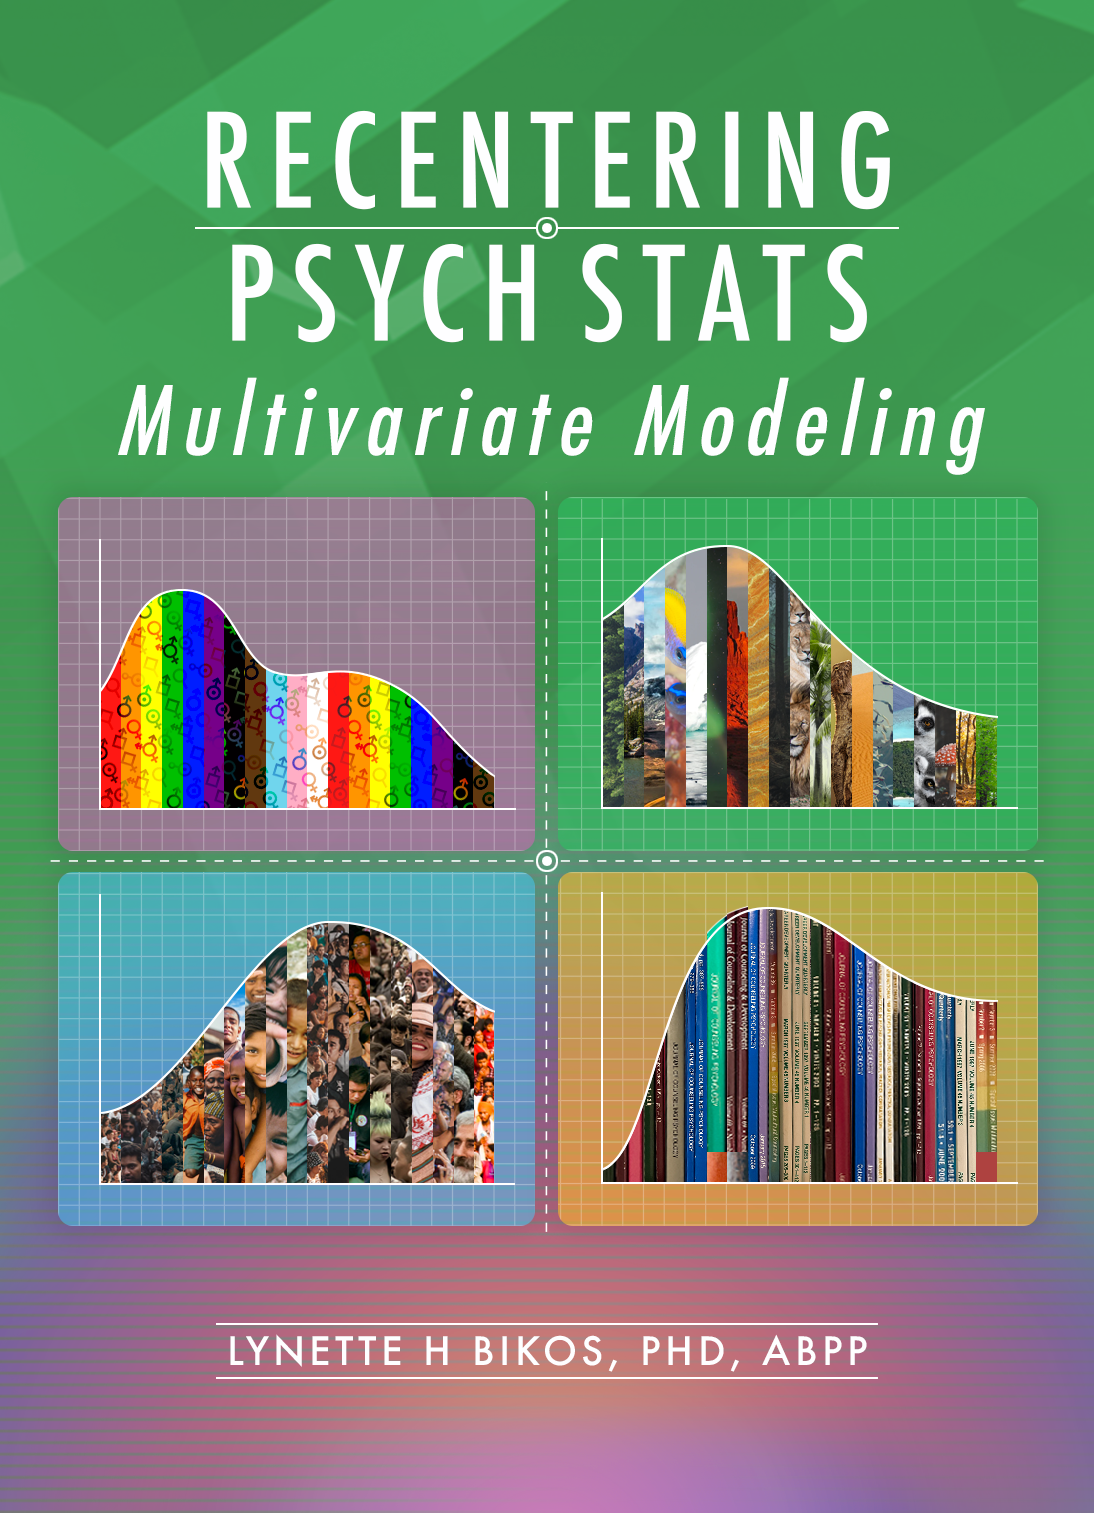
\includegraphics{images/ReC_multivariate_bkcvr.png} This open education resource is available in the following formats, all available in the \href{https://github.com/lhbikos/ReC_MultivModel/tree/main/docs}{docs} folder at the GitHub repository:

\begin{itemize}
\tightlist
\item
  Formatted as an \href{https://lhbikos.github.io/ReC_MultivModel/}{html book} via GitHub Pages available
\item
  As a \href{https://github.com/lhbikos/ReC_MultivModel/blob/main/docs/ReC_MultMod.pdf}{PDF}
\item
  As an \href{https://github.com/lhbikos/ReC_MultivModel/blob/main/docs/ReC_MultMod.epub}{ebook}
\item
  As a \href{https://github.com/lhbikos/ReC_MultivModel/blob/main/docs/ReC_MultMod.docx}{Word}
\end{itemize}

All materials used in creating this OER are available at its \href{https://github.com/lhbikos/ReC_MultivModel}{GitHub repo}.

\hypertarget{preface}{%
\chapter*{PREFACE}\label{preface}}


\textbf{If you are viewing this document, you should know that this is a book-in-progress. Early drafts are released for the purpose teaching my classes and gaining formative feedback from a host of stakeholders. The document was last updated on 12 Nov 2023}. Emerging volumes on other statistics are posted on the \href{https://lhbikos.github.io/BikosRVT/ReCenter.html}{ReCentering Psych Stats} page at my research team's website.

\href{https://spu.hosted.panopto.com/Panopto/Pages/Viewer.aspx?id=c932455e-ef06-444a-bdca-acf7012d759a}{Screencasted Lecture Link}

To \emph{center} a variable in regression means to set its value at zero and interpret all other values in relation to this reference point. Regarding race and gender, researchers often center male and White at zero. Further, it is typical that research vignettes in statistics textbooks are similarly seated in a White, Western (frequently U.S.), heteronormative, framework. The purpose of this project is to create a set of open educational resources (OER) appropriate for doctoral and post-doctoral training that contribute to a socially responsive pedagogy -- that is, it contributes to justice, equity, diversity, and inclusion.

Statistics training in doctoral programs are frequently taught with fee-for-use programs (e.g., SPSS/AMOS, SAS, MPlus) that may not be readily available to the post-doctoral professional. In recent years, there has been an increase and improvement in R packages (e.g., \emph{psych}, \emph{lavaan}) used for in analyses common to psychological research. Correspondingly, many graduate programs are transitioning to statistics training in R (free and open source). This is a challenge for post-doctoral psychologists who were trained with other software. This OER will offer statistics training with R and be freely available (specifically in a GitHub respository and posted through GitHub Pages) under a Creative Commons Attribution - Non Commercial - Share Alike license {[}CC BY-NC-SA 4.0{]}.

Training models for doctoral programs in HSP are commonly scholar-practitioner, scientist-practitioner, or clinical-scientist. An emerging model, the \emph{scientist-practitioner-advocacy} training model incorporates social justice advocacy so that graduates are equipped to recognize and address the sociocultural context of oppression and unjust distribution of resources and opportunities \citep{mallinckrodt_scientist-practitioner-advocate_2014}. In statistics textbooks, the use of research vignettes engages the learner around a tangible scenario for identifying independent variables, dependent variables, covariates, and potential mechanisms of change. Many students recall examples in Field's \citeyearpar{field_discovering_2012} popular statistics text: Viagra to teach one-way ANOVA, beer goggles for two-way ANOVA, and bushtucker for repeated measures. What if the research vignettes were more socially responsive?

In this OER, research vignettes will be from recently published articles where:

\begin{itemize}
\tightlist
\item
  the author's identity is from a group where scholarship is historically marginalized (e.g., BIPOC, LGBTQ+, LMIC{[}low-middle income countries{]}),
\item
  the research is responsive to issues of justice, equity, inclusion, diversity,
\item
  the lesson's statistic is used in the article, and
\item
  there is sufficient information in the article to simulate the data for the chapter example(s) and practice problem(s); or it is publicly available.
\end{itemize}

In training for multicultural competence, the saying, ``A fish doesn't know that it's wet'' is often used to convey the notion that we are often unaware of our own cultural characteristics. In recent months and years, there has been an increased awakening to the institutional and systemic racism that our systems are perpetuating. Queuing from the water metaphor, I am hopeful that a text that is recentered in the ways I have described can contribute to \emph{changing the water} in higher education and in the profession of psychology.

\hypertarget{copyright-with-open-access}{%
\section*{Copyright with Open Access}\label{copyright-with-open-access}}


This book is published under a a Creative Commons Attribution-NonCommercial-ShareAlike 4.0 International License. This means that this book can be reused, remixed, retained, revised and redistributed (including commercially) as long as appropriate credit is given to the authors. If you remix, or modify the original version of this open textbook, you must redistribute all versions of this open textbook under the same license - CC BY-SA.

A \href{https://github.com/lhbikos/ReC_MultivModel}{GitHub open-source repository} contains all of the text and source code for the book, including data and images.

\hypertarget{acknowledgements}{%
\chapter*{ACKNOWLEDGEMENTS}\label{acknowledgements}}


As a doctoral student at the University of Kansas (1992-2005), I learned that ``a foreign language'' was a graduation requirement. \emph{Please note that as one who studies the intersections of global, vocational, and sustainable psychology, I regret that I do not have language skills beyond English.} This could have been met with credit from high school my rural, mid-Missouri high school did not offer such classes. This requirement would have typically been met with courses taken during an undergraduate program -- but my non-teaching degree in the University of Missouri's School of Education was exempt from this. The requirement could have also been met with a computer language (fortran, C++) -- I did not have any of those either. There was a tiny footnote on my doctoral degree plan that indicated that a 2-credit course, ``SPSS for Windows'' would substitute for the language requirement. Given that it was taught by my one of my favorite professors, I readily signed up. As it turns out, Samuel B. Green, PhD, was using the course to draft chapters in the textbook \citep{green_using_2017} that has been so helpful for so many. Unfortunately, Drs. Green (1947 - 2018) and Salkind (2947 - 2017) are no longer with us. I have worn out numerous versions of their text. Another favorite text of mine was Dr.~Barbara Byrne's \citeyearpar{byrne_structural_2016}, ``Structural Equation Modeling with AMOS.'' I loved the way she worked through each problem and paired it with a published journal article, so that the user could see how the statistical evaluation fit within the larger project/article. I took my tea-stained text with me to a workshop she taught at APA and was proud of the signature she added to it (a little catfur might have fallen out). Dr.~Byrne created SEM texts for a number of statistical programs (e.g., LISREL, EQS, MPlus). As I was learning R, I wrote Dr.~Byrne, asking if she had an edition teaching SEM/CFA with R. She promptly wrote back, saying that she did not have the bandwidth to learn a new statistics package. We lost Dr.~Byrne in December 2020. I am so grateful to these role models for their contributions to my statistical training. I am also grateful for the doctoral students who have taken my courses and are continuing to provide input for how to improve the materials.

The inspiration for training materials that re*center statistics and research methods came from the \href{https://www.academics4blacklives.com/}{Academics for Black Survival and Wellness Initiative}. This project, co-founded by Della V. Mosley, Ph.D., and Pearis L. Bellamy, M.S., made clear the necessity and urgency for change in higher education and the profession of psychology.

At very practical levels, I am indebted to SPU's Library, and more specifically, SPU's Education, Technology, and Media Department. Assistant Dean for Instructional Design and Emerging Technologies, R. John Robertson, MSc, MCS, has offered unlimited consultation, support, and connection. Senior Instructional Designer in Graphics \& Illustrations, Dominic Wilkinson, designed the logo and bookcover. Psychology and Scholarly Communications Librarian, Kristin Hoffman, MLIS, has provided consultation on topics ranging from OERS to citations. I am alo indebted to Associate Vice President, Teaching and Learning at Kwantlen Polytechnic University, Rajiv Jhangiani, PhD. Dr.~Jhangiani's text \citeyearpar{jhangiani_research_2019} was the first OER I ever used and I was grateful for his encouraging conversation.

Financial support for this project has been provided the following:

\begin{itemize}
\tightlist
\item
  \emph{Call to Action on Equity, Inclusion, Diversity, Justice, and Social Responsivity Request for Proposals} grant from the Association of Psychology Postdoctoral and Internship Centers (2021-2022).
\item
  \emph{Diversity Seed Grant}, Office of Inclusive Excellence and Advisory Council for Diversity and Reconciliation (ACDR), Seattle Pacific University.
\item
  \emph{ETM Open Textbook \& OER Development Funding}, Office of Education, Technology, \& Media, Seattle Pacific University.
\end{itemize}

\hypertarget{dataprep}{%
\chapter*{DATA PREP}\label{dataprep}}


\hypertarget{scrub}{%
\chapter{Scrubbing}\label{scrub}}

\href{https://youtube.com/playlist?list=PLtz5cFLQl4KPwGvx4MHxA7C1StPkHnFH3\&si=VzB-HVlJTS07FuFw}{Screencasted Lecture Link}

The focus of this chapter is the process of starting with raw data and preparing it for multivariate analysis. To that end, we will address the conceptual considerations and practical steps in ``scrubbing and scoring.''

A twist in this lesson is that I am asking you to contribute to the dataset that serves as the basis for the chapter and the practice problems. In the spirit of \emph{open science}, this dataset is available to you and others for your own learning. Before continuing, please take 15-20 minutes to complete the survey titled, \href{https://spupsych.az1.qualtrics.com/jfe/form/SV_b2cClqAlLGQ6nLU}{Rate-a-Recent-Course: A ReCentering Psych Stats Exercise}. The study is approved by the Institutional Review Board at Seattle Pacific University (SPUIRB\# 202102011, no expiration). Details about the study, including an informed consent, are included at the link.

\hypertarget{navigating-this-lesson}{%
\section{Navigating this Lesson}\label{navigating-this-lesson}}

There is about 90 minutes of lecture. If you work through the materials with me it would be good to add another hour.

While the majority of R objects and data you will need are created within the R script that sources the chapter, there are a few that cannot be created from within the R framework. Additionally, sometimes links fail. All original materials are provided at the \href{https://github.com/lhbikos/ReC_MultivModel}{Github site} that hosts the book. More detailed guidelines for ways to access all these materials are provided in the OER's \protect\hyperlink{ReCintro}{introduction}

\hypertarget{learning-objectives}{%
\subsection{Learning Objectives}\label{learning-objectives}}

Learning objectives from this lecture include the following:

\begin{itemize}
\tightlist
\item
  Import data from Qualtrics into R.
\item
  Apply inclusion and exclusion criteria to a dataset.
\item
  Rename variables.
\item
  Create a smaller dataframe with variables appropriate for testing a specific statistical model.
\item
  Use critical data manipulation functions from the \emph{tidyverse} (and \emph{dplyr}) in particular such as \emph{filter()}, \emph{select()}, and \emph{mutate()} to prepare variables.
\item
  Articulate the initial steps in a workflow for scrubbing and scoring data.
\end{itemize}

\hypertarget{planning-for-practice}{%
\subsection{Planning for Practice}\label{planning-for-practice}}

The suggestions for practice will start with this chapter and continue in the next two chapters (Scoring, Data Dx). Using Parent's \citeyearpar{parent_handling_2013} AIA (available item analysis) approach to managing missing data, you will scrub-and-score a raw dataset. Options of graded complexity could incude:

\begin{itemize}
\tightlist
\item
  Repeating the steps in the chapter with the most recent data from the Rate-A-Recent-Course survey; differences will be in the number of people who have completed the survey since the chapter was written.
\item
  Use the dataset that is the source of the chapter, but score a different set of items that you choose.
\item
  Begin with raw data to which you have access.
\end{itemize}

\hypertarget{readings-resources}{%
\subsection{Readings \& Resources}\label{readings-resources}}

In preparing this chapter, I drew heavily from the following resource(s). Other resources are cited (when possible, linked) in the text with complete citations in the reference list.

\begin{itemize}
\tightlist
\item
  Parent, M. C. (2013). Handling item-level missing data: Simpler is just as good. The Counseling Psychologist, 41(4), 568--600. \url{https://doi.org/10.1177/0011000012445176}

  \begin{itemize}
  \tightlist
  \item
    The purpose of Parent's article was to argue that complex and resource-intensive procedurs like multiple imputation are unnecessary. Following a simulation that supports his claims, Parent provides some guidelines to follow for the AIA approach.
  \end{itemize}
\item
  Kline, R. B. (2016). Data preparation and psychometrics review. In Principles and Practice of Structural Equation Modeling, Fourth Edition. Guilford Publications. \url{http://ebookcentral.proquest.com/lib/spu/detail.action?docID=4000663}

  \begin{itemize}
  \tightlist
  \item
    Kline's chapter is my ``go-to'' for making decisions about preparing data for analysis.
  \end{itemize}
\end{itemize}

\hypertarget{packages}{%
\subsection{Packages}\label{packages}}

The script below will (a) check to see if the following packages are installed on your computer and, if not (b) install them.

\begin{Shaded}
\begin{Highlighting}[]
\CommentTok{\# will install the package if not already installed}
\CommentTok{\# if(!require(qualtRics))\{install.packages(\textquotesingle{}qualtRics\textquotesingle{})\}}
\CommentTok{\# if(!require(tidyverse))\{install.packages(\textquotesingle{}tidyverse\textquotesingle{})\}}
\end{Highlighting}
\end{Shaded}

\hypertarget{workflow-for-scrubbing}{%
\section{Workflow for Scrubbing}\label{workflow-for-scrubbing}}

The same workflow guides us through the Scrubbing, Scoring, and Data Dx chapters. In this lesson we focus on downloading data from Qualtrics and determining which cases can be retained for analysis based on inclusion and exclusion criteria.

\begin{figure}
\centering
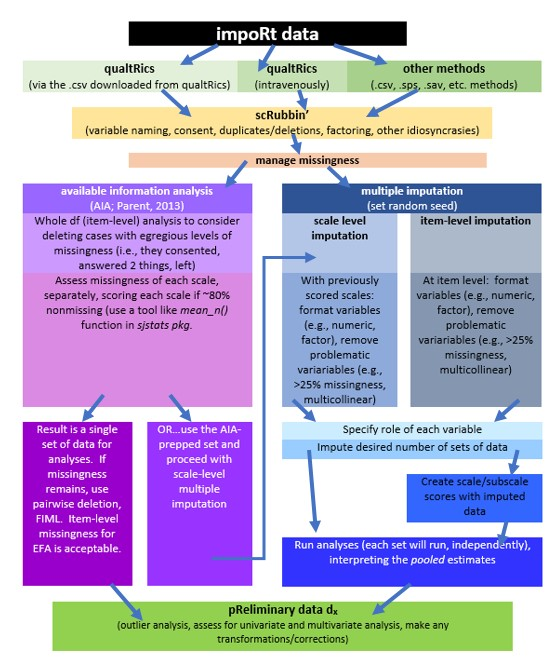
\includegraphics{images/Ch02/scrubscore_wrkflow.jpg}
\caption{An image of a workflow for scrubbing and scoring data.}
\end{figure}

Here is a narration of the figure:

\begin{enumerate}
\def\labelenumi{\arabic{enumi}.}
\tightlist
\item
  The workflow begins by importing data into R. Most lessons in this series involve simulated data that are created directly in R. Alternatively, data could be:

  \begin{itemize}
  \tightlist
  \item
    imported ``intRavenously'' through programs such as Qualtrics,
  \item
    exported from programs such as Qualtrics to another program (e.g., .xlxs, .csv),
  \item
    imported in other forms (e.g., .csv, .sps, .sav).
  \end{itemize}
\item
  Scrubbing data by

  \begin{itemize}
  \tightlist
  \item
    variable naming,
  \item
    specifying variable characteristics such as factoring,
  \item
    ensuring that included participants consented to participation,
  \item
    determining and executing the inclusion and exclusion criteria.
  \end{itemize}
\item
  Conduct preliminary data diagnostics such as

  \begin{itemize}
  \tightlist
  \item
    outlier analysis
  \item
    assessing for univariate and multivariate analysis
  \item
    making transformations and/or corrections
  \end{itemize}
\item
  Managing missingness by one of two routes

  \begin{itemize}
  \tightlist
  \item
    Available information analysis \citep{parent_handling_2013} at either the item-level or scale level. The result is a single set of data for analysis. If missingness remains, options include pairwise deletion, listwise deletion, or specifying FIML (when available). Another option is to use multiple imputation.
  \item
    Multiple imputation at either scale level or item-level
  \end{itemize}
\end{enumerate}

\hypertarget{research-vignette}{%
\section{Research Vignette}\label{research-vignette}}

To provide first-hand experience as both the respondent and analyst for the same set of data, you were asked to complete a survey titled, \href{https://spupsych.az1.qualtrics.com/jfe/form/SV_b2cClqAlLGQ6nLU}{Rate-a-Recent-Course: A ReCentering Psych Stats Exercise}. If you haven't yet completed it, please consider doing so, now. In order to reduce the potential threats to validity by providing background information about the survey, I will wait to describe it until later in the chapter.

The survey is administered in Qualtrics. In the chapter I teach two ways to import Qualtrics data into R. We will then use the data to work through the steps identified in the workflow.

\hypertarget{working-the-problem}{%
\section{Working the Problem}\label{working-the-problem}}

\hypertarget{intravenous-qualtrics}{%
\subsection{intRavenous Qualtrics}\label{intravenous-qualtrics}}

I will demonstrate using a Qualtrics account at my institution, Seattle Pacific University. The only surveys in this account are for the \emph{Recentering Psych Stats} chapters and lessons. The surveys were designed to not capture personally identifying information.

Access credentials for the institutional account, individual user's account, and survey are essential for getting the survey items and/or results to export into R. The Qualtrics website provides a tutorial for \href{https://www.qualtrics.com/support/integrations/api-integration/overview/\#GeneratingAnAPIToken}{generating an API token}.

We need two pieces of information: the \textbf{root\_url} and an \textbf{API token}. To retrieve these:

\begin{itemize}
\tightlist
\item
  Log into your respective qualtrics.com account
\item
  Select Account Settings
\item
  Choose ``Qualtrics IDs'' from the user name dropdown
\end{itemize}

The \textbf{root\_url} is the first part of the web address for the Qualtrics account. For our institution it is: \emph{spupsych.az1.qualtrics.com }.

The API token is in the box labeled, ``API.'' If it is empty, select, ``Generate Token.'' If you do not have this option, locate the \emph{brand administrator} for your Qualtrics account. They will need to set up your account so that you have API privileges.

\emph{BE CAREFUL WITH THE API TOKEN} This is the key to your Qualtrics accounts. If you leave it in an .rmd file that you forward to someone else or upload to a data repository, this key and the base URL gives access to every survey in your account. If you share it, you could be releasing survey data to others that would violate confidentiality promises in an IRB application.

If you mistakenly give out your API token you can generate a new one within your Qualtrics account and re-protect all its contents.

You do need to change the API key/token if you want to download data from a different Qualtrics account. If your list of surveys generates the wrong set of surveys, restart R, make sure you have the correct API token and try again.

\begin{Shaded}
\begin{Highlighting}[]
\CommentTok{\# You only need to run this ONCE to draw from the same Qualtrics}
\CommentTok{\# account. If you change Qualtrics accounts you will need to get a}
\CommentTok{\# different token.}

\CommentTok{\# qualtRics::qualtrics\_api\_credentials(api\_key =}
\CommentTok{\# \textquotesingle{}mUgPMySYkiWpMFkwHale1QE5HNmh5LRUaA8d9PDg\textquotesingle{}, base\_url =}
\CommentTok{\# \textquotesingle{}spupsych.az1.qualtrics.com\textquotesingle{}, overwrite = TRUE, install = TRUE)}

\CommentTok{\# readRenviron(\textquotesingle{}\textasciitilde{}/.Renviron\textquotesingle{})}
\end{Highlighting}
\end{Shaded}

\emph{all\_surveys()} generates a dataframe containing information about all the surveys stored on your Qualtrics account.

\begin{Shaded}
\begin{Highlighting}[]
\CommentTok{\# surveys \textless{}{-} qualtRics::all\_surveys()}

\CommentTok{\# View this as an object (found in the right: Environment).  Get}
\CommentTok{\# survey id \# for the next command If this is showing you the WRONG}
\CommentTok{\# list of surveys, you are pulling from the wrong Qualtrics account}
\CommentTok{\# (i.e., maybe this one instead of your own). Go back and change your}
\CommentTok{\# API token (it saves your old one). Changing the API likely requires}
\CommentTok{\# a restart of R.}
\end{Highlighting}
\end{Shaded}

To retrieve the survey, use the \emph{fetch\_survey()} function.

\begin{Shaded}
\begin{Highlighting}[]
\CommentTok{\# obtained with the survey ID}
\CommentTok{\#\textquotesingle{}surveyID\textquotesingle{} should be the ID from above}
\CommentTok{\#\textquotesingle{}verbose\textquotesingle{} prints messages to the R console}
\CommentTok{\#\textquotesingle{}label\textquotesingle{}, when TRUE, imports data as text responses; if FALSE prints the data as numerical responses}
\CommentTok{\#\textquotesingle{}convert\textquotesingle{}, when TRUE, attempts to convert certain question types to the \textquotesingle{}proper\textquotesingle{} data type in R; because I don\textquotesingle{}t like guessing, I want to set up my own factors.}
\CommentTok{\#\textquotesingle{}force\_request\textquotesingle{}, when TRUE, always downloads the survey from the API instead of from a temporary directory (i.e., it always goes to the primary source)}
\CommentTok{\# \textquotesingle{}import\_id\textquotesingle{}, when TRUE includes the unique Qualtrics{-}assigned ID;}
\CommentTok{\# since I have provided labels, I want false}

\CommentTok{\# QTRX\_df \textless{}{-}qualtRics::fetch\_survey(surveyID = \textquotesingle{}SV\_b2cClqAlLGQ6nLU\textquotesingle{},}
\CommentTok{\# time\_zone = NULL, verbose = FALSE, label=FALSE, convert=FALSE,}
\CommentTok{\# force\_request = TRUE, import\_id = FALSE)}

\CommentTok{\# useLocalTime = TRUE,}
\end{Highlighting}
\end{Shaded}

\emph{It is possible to import Qualtrics data that has been downloaded from Qualtrics as a .csv. I demo this in the Bonus Reel at the end of this lesson.}

In prior versions of this chapter I allowed the chapter to automatically update with ``all the new data'' each time the OER was re-rendered/built. Because I think this caused confusion, I have decided to save the data in both .csv and .rds versions, then clear my environment, upload the .rds (my personal favorite format) version, and demonstrate the scrubbing techniques with that data. If you continue with data you just downloaded from Qualtrics, you will get different answers than are in the lesson. While I think that continuing with the most current data set is a viable option for a practice problem, it could be confusing. Rather, follow one of the two options below to upload .csv or .rds versions of the data I used in the lesson.

\hypertarget{option-1.-upload-an-.rds-file}{%
\subsubsection{Option 1. Upload an .rds file}\label{option-1.-upload-an-.rds-file}}

Because .rds files will retain any formatting information we provide about variables, I like using them. The downside is that you cannot simply open and view them outside of the R environment. Here is the code I used to produce the .rds version of the file. If you want to obtain the same results as I report in the chapter, do NOT run it again.

\begin{Shaded}
\begin{Highlighting}[]
\CommentTok{\# to save the df as an .rds (think \textquotesingle{}R object\textquotesingle{}) file on your computer;}
\CommentTok{\# it should save in the same file as the .rmd file you are working}
\CommentTok{\# with saveRDS(QTRX\_df, \textquotesingle{}QTRX\_df230902.rds\textquotesingle{})}
\end{Highlighting}
\end{Shaded}

Rather, head to the \href{https://github.com/lhbikos/ReC_MultivModel}{MultivModel GitHub} site and download the \emph{QTRX\_df230902b.rds} file. Place it in the same folder as the .rmd you are using and run the code below. And actually, I further re-named the file that you will retrieve so that it won't be over-written.*

\begin{Shaded}
\begin{Highlighting}[]
\NormalTok{QTRX\_df }\OtherTok{\textless{}{-}} \FunctionTok{readRDS}\NormalTok{(}\StringTok{"QTRX\_df230902b.rds"}\NormalTok{)}
\end{Highlighting}
\end{Shaded}

Occasionally, I have had a student for whom the .rds files don't seem to work. Uploading a .csv file is an option.

\hypertarget{option-2.-upload-a-.csv-file}{%
\subsubsection{Option 2. Upload a .csv file}\label{option-2.-upload-a-.csv-file}}

Simply for your information, here is the code I used to produce the .csv version of the file. If you want to obtain the same results as I report in the chapter, do NOT run it again.

\begin{Shaded}
\begin{Highlighting}[]
\CommentTok{\# write the simulated data as a .csv write.table(QTRX\_df,}
\CommentTok{\# file=\textquotesingle{}QTRX\_df230902.csv\textquotesingle{}, sep=\textquotesingle{},\textquotesingle{}, col.names=TRUE, row.names=FALSE)}
\end{Highlighting}
\end{Shaded}

Rather, head to the \href{https://github.com/lhbikos/ReC_MultivModel}{MultivModel GitHub} site and download the \emph{QTRX\_df230902b.csv} file. Place it in the same folder as the .rmd you are using and run the code below. \emph{And actually, I further re-named the file that you will retrieve so that it won't be over-written.}

\begin{Shaded}
\begin{Highlighting}[]
\CommentTok{\# bring back the simulated dat from a .csv file QTRX\_df \textless{}{-}}
\CommentTok{\# read.csv(\textquotesingle{}QTRX\_df230902b.csv\textquotesingle{}, header = TRUE)}
\end{Highlighting}
\end{Shaded}

You need not do both. That is, either download-and-import either the .rds or .csv file.

\hypertarget{about-the-rate-a-recent-course-survey}{%
\subsection{\texorpdfstring{About the \emph{Rate-a-Recent-Course} Survey}{About the Rate-a-Recent-Course Survey}}\label{about-the-rate-a-recent-course-survey}}

As a teaching activity for the ReCentering Psych Stats OER, the topic of the survey was selected to be consistent with the overall theme of OER. Specifically, the purpose of this study is to understand the campus climate for students whose identities make them vulnerable to bias and discrimination. These include students who are Black, non-Black students of color, LGBTQ+ students, international students, and students with disabilities.

Although the dataset should provide the opportunity to test a number of statistical models, one working hypothesis that framed the study is that the there will be a greater sense of belonging and less bias and discrimination when there is similar representation (of identities that are often marginalized) in the instructional faculty and student body. Termed, ``structural diversity'' \citep{lewis_black_2019} this is likely an oversimplification. In fact, an increase in diverse representation without attention to interacting factors can increase hostility on campus \citep{hurtado_linking_2007}. Thus, we included the task of rating of a single course relates to the larger campus along the dimensions of belonging and bias/discrimination. For example, if a single class has higher ratings on issues of inclusivity, diversity, and respect, we would expect that sentiment to be echoed in the broader institution.

Our design has notable limitations You will likely notice that we ask about demographic characteristics of the instructional staff and classmates in the course rated, but we do not ask about the demographic characteristics of the respondent. In making this decision, we likely lose important information; Iacovino and James \citeyearpar{iacovino_retaining_2016} have noted that White students perceive campus more favorably than Black student counterparts. We made this decision to protect the identity of the respondent. As you will see when we download the data, if a faculty member asked an entire class to take the survey, the datestamp and a handful of demographic identifiers could very likely identify a student. In certain circumstances, this might be risky in that private information (i.e., gender nonconformity, disclosure of a disability) or course evaluation data could be related back to the student.

Further, the items that ask respondents to \emph{guess} the identities of the instructional staff and classmates are limited, and contrary to best practices in survey construction that recommend providing the option of a ``write-in'' a response. After consulting with a diverse group of stakeholders and subject matter experts (and revising the response options numerous times) I have attempted to center anti-Black racism in the U.S. \citep{mosley_critical_2021, mosley_radical_2020, singh_building_2020}. In fact, the display logic does not present the race items when the course is offered outside the U.S. There are only five options for race: \emph{biracial/multiracial}, \emph{Black}, \emph{non-Black person(s) of color}, \emph{White}, and \emph{I did not notice} (intended to capture a color-blind response). One unintended negative consequence of this design is that the response options could contribute to \emph{colorism} \citep{adames_fallacy_2021, capielo_rosario_acculturation_2019}. Another possibility is that the limited options may erase, or make invisible, other identities. At the time that I am writing the first draft of this chapter, the murder of six Asian American women in Atlanta has just occurred. The Center for the Study of Hate and Extremeism has documented that while overall hate crimes dropped by 7\% in 2020, anti-Asian hate crimes reported to the police in America's largest cities increasedby 149\% \citep{noauthor_fact_nodate}. These incidents have occurred not only in cities, but in our neighborhoods and on our campusus \citep{kim_guest_2021, kim_yes_2021, noauthor_stop_nodate}. While this survey is intended to assess campus climate as a function of race, it unfortunately does not distinguish between many identities that experience marginalization.

In parallel, the items asking respondents to identity characteristics of the instructional staff along dimensions of gender, international status, and disability are ``large buckets'' and do not include ``write-in'' options. Similarly, there was no intent to cause harm by erasing or making invisible individuals whose identities are better defined by different descriptors. Further, no write-in items were allowed. This was also intentional to prevent potential harm caused by people who could leave inappropriate or harmful comments.

\hypertarget{the-codebook}{%
\subsection{The Codebook}\label{the-codebook}}

In order to scrub-and-score a survey, it is critical to know about its content, scoring directions for scales/subscales, and its design. A more complete description of the survey design elements is (or will be) available in the \emph{Recentering Psych Stats: Psychometric} OER. The review in this chapter provides just-enough information to allow us to make decisions about which items to retain and how to score them. When they are well-written, information in the \href{./Bikos_ReCenteringPsychStats_ReCupload.pdf}{IRB application} and \href{https://osf.io/a8e5u}{pre-registration} can be helpful in the scrubbing and scoring process.

Let's look ``live'' at the survey. In Qualtrics it is possible to \emph{print} a PDF that looks very similar to its presentation when someone is taking it. You can access that static version \href{./Rate_a_CoursePDF.pdf}{here}.

We can export a \href{./Rate-a-Course_Codebook.pdf}{codebook}, that is, a Word (or PDF) version of the survey with all the coding. In Qualtrics the protocol is: Survey/Tools/ImportExport/Export Survey to Word. Then select all the options you want (especially ``Show Coded Values''). A tutorial provided by Qualtrics can be found \href{https://www.qualtrics.com/support/survey-platform/survey-module/survey-tools/import-and-export-surveys/}{here}. This same process can be used to print the PDF example I used above.

It is almost impossible to give this lecture without some reference to Qualtrics and the features used in Qualtrics. An import of raw data from Qualtrics into R can be nightmare in that the Qualtrics-assigned variable names are numbers (e.g., QID1, QID2) -- but often out of order because the number is assigned when the question is first created. If the survey is reordered, the numbers get out of sequence.

Similarly, values for Likert-type scales can also get out of order if the scale anchors are revised (which is common to do).

I recommend providing custom variable names and recode values directly in Qualtrics before exporting them into R. A Qualtrics tutorial for this is provided \href{https://www.qualtrics.com/support/survey-platform/survey-module/question-options/recode-values/}{here}. In general, consider these qualities when creating variable names:

\begin{itemize}
\tightlist
\item
  Brevity: historically, SPSS variable names could be a maximum of 8 characters.
\item
  Intuitive: although variables can be renamed in R (e.g., for use in charts and tables), it is helpful when the name imported from Qualtrics provides some indication of what the variable is.
\item
  Systematic: start items in a scale with the same stem, followed by the item number -- ITEM1, ITEM2, ITEM3.
\end{itemize}

The Rate-a-Recent-Course survey was written using some special features in Qualtrics. These include

\begin{itemize}
\tightlist
\item
  Display logic

  \begin{itemize}
  \tightlist
  \item
    Items that are U.S.-centric are only shown if the respondent is taking a course from an institution in the U.S. is a student in the U.S.
  \end{itemize}
\item
  Loop and merge

  \begin{itemize}
  \tightlist
  \item
    Because course may have multiple instructional staff, the information asking about demographic characteristics of the instructors is repeated according to the number input by the respondent
  \end{itemize}
\item
  Random presentation of the 30 items asking about campus climate for the five groups of students

  \begin{itemize}
  \tightlist
  \item
    Although this might increase the cognitive load of the survey, this helps ``spread out'' missingness for respondents who might tire of the survey and stop early
  \end{itemize}
\item
  Rank ordering of the institutional level (department, school/faculty, campus/university) to which the respondent feels most connected
\end{itemize}

Looking at the QTRX\_df, \emph{StartDate} thru \emph{UserLanguage} are metadata created by Qualtrics. The remaining variables and associated value labels are in the \href{./Rate-a-Course_Codebook.pdf}{codebook}.

\hypertarget{scrubbing}{%
\section{Scrubbing}\label{scrubbing}}

With a look at our survey, codebook, and imported data, we now get to the business of scRubbing (deleting those who did not give consent, deleting previews, etc.). This level of ``scrubbing'' precedes the more formal detection of outliers.

\hypertarget{tools-for-data-manipulation}{%
\subsection{Tools for Data Manipulation}\label{tools-for-data-manipulation}}

The next stages will provide some experience manipulating data with \textbf{dplyr} from the \textbf{tidyverse}.

The \textbf{tidyverse} is a system of packages (i.e,. when you download the tidyverse, you download all its packages/members) for data manipulation, exploration and visualization. The packages in the tidyverse share a common design philosophy. These were mostly developed by Hadley Wickham, but more recently, more designers are contributing to them. Tidyverse packages are intended to make statisticians and data scientists more productive by guiding them through workflows that facilitate communication and result in reproducible work products. Fundamentally, the tidyverse is about the connections between the tools that make the workflow possible. Critical packages in the tidyverse include:

\begin{itemize}
\tightlist
\item
  \textbf{dplyr}: data manipulation: mutate, select, filter, summarize, arrange
\item
  \textbf{ggplot2}: extravagant graphing
\item
  \textbf{tibble}: a \emph{tibble} is a dataframe that provides the user with more (and less) control over the data.
\item
  \textbf{readr}: gives access to ``rectangular data'' like .csv and tables
\item
  \textbf{tidyr}: tidy data is where each variable is a column, each observation is a row, each value is a cell (duh). \textbf{tidyr}'s contributions are gather(wide to long) and spread(long to wide) as well as separate, extract, unite.
\item
  \textbf{purrr}: facilitates working with functions and vectors. For example, if you write a function, using purrr may help you replace loops with code that is more efficient and intuitive.
\end{itemize}

The tidyverse is ever-evolving -- so check frequently for updates and troubleshooting.

A handy cheatsheet for data transformation is found \href{https://www.rstudio.com/wp-content/uploads/2015/02/data-wrangling-cheatsheet.pdf}{here}.

\hypertarget{inclusion-and-exclusion-criteria}{%
\subsection{Inclusion and Exclusion Criteria}\label{inclusion-and-exclusion-criteria}}

For me, the first pass at scrubbing is to eliminate the obvious. In our case this is includes \emph{previews} and respondents who did not consent to continue. Previews are the researcher-initiated responses usually designed to proofread or troubleshoot survey problems. There could be other first-pass-deletions, such as selecting response between certain dates.

I think these first-pass deletions, especially the ones around consent, are important to do as soon as possible. Otherwise, we might delete some of the variables (e.g., timestamps, consent documentation, preview status) and neglect to delete these cases later in the process.

We are here in the workflow:

\begin{figure}
\centering
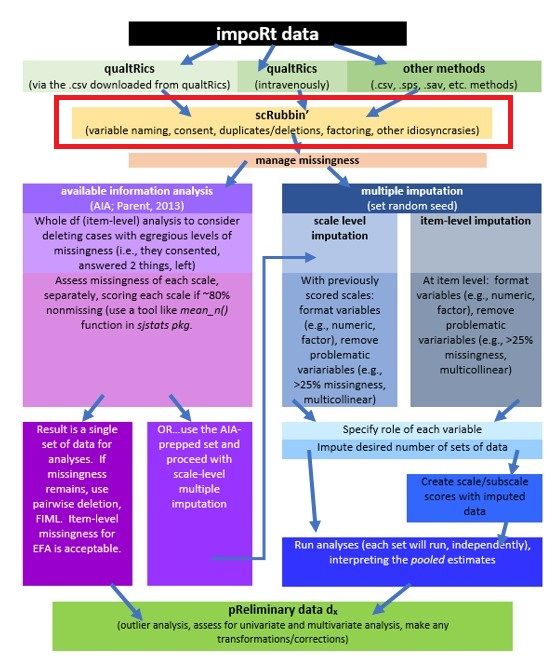
\includegraphics{images/Ch02/wrkflow_prelim.jpg}
\caption{An image of a workflow for scrubbing and scoring data.}
\end{figure}

We can either update the existing df (by using the same object), or creating a new df from the old. Either works. In my early years, I tended to create lots of new objects. As I have gained confidence in myself and in R, I'm inclined to update the existing df. Why? Because unless you write the object as an outfile (using the same name for the object as for the filename -- which I do not recommend), the object used in R does not change the source of the dat. Therefore, it is easy to correct early code and it keeps the global environment less cluttered.

In this particular survey, the majority of respondents will take the survey because they clicked an \emph{anonymous} link provided by Qualtrics. Another Qualtrics distribution method is e-mail. At the time of this writing, we have not recruited by e-mail, but it is is possible we could do so in the future. What we should not include, though, are \emph{previews}. These are the times when the researcher is self-piloting the survey to look for errors and to troubleshoot.

\begin{Shaded}
\begin{Highlighting}[]
\CommentTok{\# the filter command is used when we are making inclusion/exclusion}
\CommentTok{\# decisions about rows != means do not include cases with \textquotesingle{}preview\textquotesingle{}}

\NormalTok{QTRX\_df }\OtherTok{\textless{}{-}}\NormalTok{ dplyr}\SpecialCharTok{::}\FunctionTok{filter}\NormalTok{(QTRX\_df, DistributionChannel }\SpecialCharTok{!=} \StringTok{"preview"}\NormalTok{)}

\CommentTok{\# FYI, another way that doesn\textquotesingle{}t use tidyverse, but gets the same}
\CommentTok{\# result QTRX\_df \textless{}{-} QTRX\_df[!QTRX\_df$DistributionChannel ==}
\CommentTok{\# \textquotesingle{}preview\textquotesingle{},]}
\end{Highlighting}
\end{Shaded}

APA Style, and in particular the Journal Article Reporting Standards (JARS) for quantitative research specify that we should report the frequency or percentages of missing data. We would start our counting \emph{after} eliminating the previews.

\begin{Shaded}
\begin{Highlighting}[]
\CommentTok{\# I created an object that lists how many rows/cases remain.  I used}
\CommentTok{\# inline text below to update the text with the new number}
\FunctionTok{nrow}\NormalTok{(QTRX\_df)}
\end{Highlighting}
\end{Shaded}

\begin{verbatim}
[1] 107
\end{verbatim}

CAPTURING RESULTS FOR WRITING IT UP:

\begin{quote}
\begin{quote}
Data screening suggested that 107 individuals opened the survey link.
\end{quote}
\end{quote}

Next let's filter in only those who consented to take the survey. Because Qualtrics discontinued the survey for everyone who did not consent, we do not have to worry that their data is unintentionally included, but it can be useful to mention the number of non-consenters in the summary of missing data.

\begin{Shaded}
\begin{Highlighting}[]
\CommentTok{\# == are used}
\NormalTok{QTRX\_df }\OtherTok{\textless{}{-}}\NormalTok{ dplyr}\SpecialCharTok{::}\FunctionTok{filter}\NormalTok{(QTRX\_df, Consent }\SpecialCharTok{==} \DecValTok{1}\NormalTok{)}
\FunctionTok{nrow}\NormalTok{(QTRX\_df)}
\end{Highlighting}
\end{Shaded}

\begin{verbatim}
[1] 83
\end{verbatim}

CAPTURING RESULTS FOR WRITING IT UP:

\begin{quote}
\begin{quote}
Data screening suggested that 107 individuals opened the survey link. Of those, 83 granted consent and proceeded into the survey items.
\end{quote}
\end{quote}

In this particular study, the categories used to collect informtaion about race/ethnicity were U.S.-centric. Thus, they were only shown if the respondent indicated that the course being rated was taught by an institution in the U.S. Therefore, an an additional inclusion criteria for this specific research model should be that the course was taught in the U.S.

\begin{Shaded}
\begin{Highlighting}[]
\NormalTok{QTRX\_df }\OtherTok{\textless{}{-}}\NormalTok{dplyr}\SpecialCharTok{::}\FunctionTok{filter}\NormalTok{(QTRX\_df, USinst }\SpecialCharTok{==} \DecValTok{0}\NormalTok{)}
\FunctionTok{nrow}\NormalTok{(QTRX\_df)}
\end{Highlighting}
\end{Shaded}

\begin{verbatim}
[1] 69
\end{verbatim}

CAPTURING RESULTS FOR WRITING IT UP:

\begin{quote}
\begin{quote}
Data screening suggested that 107 individuals opened the survey link. Of those, 83 granted consent and proceeded into the survey items. A further inclusion criteria was that the course was taught in the U.S; 69 met this criteria.
\end{quote}
\end{quote}

\hypertarget{renaming-variables}{%
\subsection{Renaming Variables}\label{renaming-variables}}

Even though we renamed the variables in Qualtrics, the loop-and-merge variables were auto-renamed such that they each started with a number. I cannot see how to rename these from inside Qualtrics. A potential problem is that, in R, when variable names start with numbers, they need to be surrounded with single quotation marks. I find it easier to rename them now. I used ``i'' to start the variable name to represent ``instructor.''

The form of the \emph{rename()} function is this: df\_named \textless- rename(df\_raw, NewName1 = OldName1)

\begin{Shaded}
\begin{Highlighting}[]
\NormalTok{QTRX\_df }\OtherTok{\textless{}{-}}\NormalTok{ dplyr}\SpecialCharTok{::}\FunctionTok{rename}\NormalTok{(QTRX\_df, }\AttributeTok{iRace1 =} \StringTok{"1\_iRace"}\NormalTok{, }\AttributeTok{iRace2 =} \StringTok{"2\_iRace"}\NormalTok{,}
    \AttributeTok{iRace3 =} \StringTok{"3\_iRace"}\NormalTok{, }\AttributeTok{iRace4 =} \StringTok{"4\_iRace"}\NormalTok{, }\AttributeTok{iRace5 =} \StringTok{"5\_iRace"}\NormalTok{, }\AttributeTok{iRace6 =} \StringTok{"6\_iRace"}\NormalTok{,}
    \AttributeTok{iRace7 =} \StringTok{"7\_iRace"}\NormalTok{, }\AttributeTok{iRace8 =} \StringTok{"8\_iRace"}\NormalTok{, }\AttributeTok{iRace9 =} \StringTok{"9\_iRace"}\NormalTok{, }\AttributeTok{iRace10 =} \StringTok{"10\_iRace"}\NormalTok{)}
\end{Highlighting}
\end{Shaded}

Also in Qualtrics, it was not possible to rename the variable (formatted with sliders) that asked respondents to estimate the proportion of classmates in each race-based category. Using the codebook, we can do this now. I will use ``cm'' to precede each variable name to represent ``classmates.''

\begin{Shaded}
\begin{Highlighting}[]
\NormalTok{QTRX\_df }\OtherTok{\textless{}{-}}\NormalTok{ dplyr}\SpecialCharTok{::}\FunctionTok{rename}\NormalTok{(QTRX\_df, }\AttributeTok{cmBiMulti =}\NormalTok{ Race\_10, }\AttributeTok{cmBlack =}\NormalTok{ Race\_1,}
    \AttributeTok{cmNBPoC =}\NormalTok{ Race\_7, }\AttributeTok{cmWhite =}\NormalTok{ Race\_8, }\AttributeTok{cmUnsure =}\NormalTok{ Race\_2)}
\end{Highlighting}
\end{Shaded}

Let's also create an ID variable (different from the lengthy Qualtrics-issued ID) and then move it to the front of the distribution.

\begin{Shaded}
\begin{Highlighting}[]
\CommentTok{\# Opening the tidyverse so that I can use pipes}
\FunctionTok{library}\NormalTok{(tidyverse)}
\end{Highlighting}
\end{Shaded}

\begin{verbatim}
-- Attaching core tidyverse packages ------------------------ tidyverse 2.0.0 --
v dplyr     1.1.2     v readr     2.1.4
v forcats   1.0.0     v stringr   1.5.0
v ggplot2   3.4.3     v tibble    3.2.1
v lubridate 1.9.2     v tidyr     1.3.0
v purrr     1.0.1     
-- Conflicts ------------------------------------------ tidyverse_conflicts() --
x dplyr::filter() masks stats::filter()
x dplyr::lag()    masks stats::lag()
i Use the conflicted package (<http://conflicted.r-lib.org/>) to force all conflicts to become errors
\end{verbatim}

\begin{Shaded}
\begin{Highlighting}[]
\NormalTok{QTRX\_df }\OtherTok{\textless{}{-}}\NormalTok{ QTRX\_df }\SpecialCharTok{\%\textgreater{}\%}
\NormalTok{    dplyr}\SpecialCharTok{::}\FunctionTok{mutate}\NormalTok{(}\AttributeTok{ID =} \FunctionTok{row\_number}\NormalTok{())}

\CommentTok{\# moving the ID number to the first column; requires}
\NormalTok{QTRX\_df }\OtherTok{\textless{}{-}}\NormalTok{ QTRX\_df }\SpecialCharTok{\%\textgreater{}\%}
\NormalTok{    dplyr}\SpecialCharTok{::}\FunctionTok{select}\NormalTok{(ID, }\FunctionTok{everything}\NormalTok{())}
\end{Highlighting}
\end{Shaded}

\hypertarget{downsizing-the-dataframe}{%
\subsection{Downsizing the Dataframe}\label{downsizing-the-dataframe}}

Although researchers may differ in their approach, my tendency is to downsize the df to the variables I will be using in my study. These could include variables in the model, demographic variables, and potentially auxiliary variables (i.e,. variables not in the model, but that might be used in the case of multiple imputation).

This particular survey did not collect demographic information, so that will not be used. The model that I will demonstrate in this research vignette examines the the respondent's perceived campus climate for students who are Black, predicted by the the respondent's own campus belonging, and also the \emph{structural diversity} \citep{lewis_black_2019} proportions of Black students in the classroom and BIPOC (Black, Indigenous, and people of color) instructional staff.

\emph{I would like to assess the model by having the instructional staff variable to be the \%Black instructional staff. At the time that this lecture is being prepared, there is not sufficient Black representation in the staff to model this.}

The \emph{select()} function can let us list the variables we want to retain.

\begin{Shaded}
\begin{Highlighting}[]
\CommentTok{\# You can use the \textquotesingle{}:\textquotesingle{} to include all variables from the first to last}
\CommentTok{\# variable in any sequence; I could have written this more}
\CommentTok{\# efficiently.  I just like to \textquotesingle{}see\textquotesingle{} my scales and clusters of}
\CommentTok{\# variables.}

\NormalTok{Model\_df }\OtherTok{\textless{}{-}}\NormalTok{ (dplyr}\SpecialCharTok{::}\FunctionTok{select}\NormalTok{(QTRX\_df, ID, iRace1, iRace2, iRace3, iRace4,}
\NormalTok{    iRace5, iRace6, iRace7, iRace8, iRace9, iRace10, cmBiMulti, cmBlack,}
\NormalTok{    cmNBPoC, cmWhite, cmUnsure, Belong\_1}\SpecialCharTok{:}\NormalTok{Belong\_3, Blst\_1}\SpecialCharTok{:}\NormalTok{Blst\_6))}
\end{Highlighting}
\end{Shaded}

It can be helpful to save outfile of progress as we go along. Here I save this raw file. I will demonstrate how to save both .rds and .csv files.

\begin{Shaded}
\begin{Highlighting}[]
\CommentTok{\# to save the df as an .rds (think \textquotesingle{}R object\textquotesingle{}) file on your computer;}
\CommentTok{\# it should save in the same file as the .rmd file you are working}
\CommentTok{\# with saveRDS(Model\_df, \textquotesingle{}BlackStntsModel230902.rds\textquotesingle{}) code to import}
\CommentTok{\# that model we just saved Model\_df \textless{}{-}}
\CommentTok{\# readRDS(\textquotesingle{}BlackStntsModel230902.rds\textquotesingle{})}
\end{Highlighting}
\end{Shaded}

\begin{Shaded}
\begin{Highlighting}[]
\CommentTok{\# write the simulated data as a .csv write.table(Model\_df,}
\CommentTok{\# file=\textquotesingle{}BlackStntsModel230902.csv\textquotesingle{}, sep=\textquotesingle{},\textquotesingle{}, col.names=TRUE,}
\CommentTok{\# row.names=FALSE) bring back the simulated data from a .csv file}
\CommentTok{\# Model\_df \textless{}{-} read.csv(\textquotesingle{}BlackStntsModel230902.csv\textquotesingle{}, header = TRUE)}
\end{Highlighting}
\end{Shaded}

\hypertarget{toward-the-apa-style-write-up}{%
\section{Toward the APA Style Write-up}\label{toward-the-apa-style-write-up}}

Because we have been capturing the results as we have worked the problem, our results section is easy to assemble.

\hypertarget{methodprocedure}{%
\subsection{Method/Procedure}\label{methodprocedure}}

\begin{quote}
\begin{quote}
Data screening suggested that 107 individuals opened the survey link. Of those, 83 granted consent and proceeded into the survey items. A further inclusion criteria was that the course was taught in the U.S; 69 met this criteria.
\end{quote}
\end{quote}

\hypertarget{practice-problems}{%
\section{Practice Problems}\label{practice-problems}}

Starting with this chapter, the practice problems for this and the next two chapters (i.e., Scoring, Data Dx) are intended to be completed in a sequence. Whatever practice option(s) you choose, please

\begin{itemize}
\tightlist
\item
  Use raw data that has some missingness (as a last resort you could manually delete some cells),
\item
  Includes at least 3 independent/predictor variables

  \begin{itemize}
  \tightlist
  \item
    these could be categorically or continuously scaled
  \item
    at least one variable should require scoring.
  \end{itemize}
\item
  Include at least 1 dependent variable

  \begin{itemize}
  \tightlist
  \item
    at this point in your learning it should be continuously scaled
  \end{itemize}
\end{itemize}

The three problems below are listed in the order of graded complexity. If you are just getting started, you may wish to start with the first problem. If you are more confident, choose the second or third option. You will likely encounter challenges that were not covered in this chapter. Search for and try out solutions, knowing that there are multiple paths through the analysis.

\hypertarget{problem-1-rework-the-chapter-problem}{%
\subsection{Problem \#1: Rework the Chapter Problem}\label{problem-1-rework-the-chapter-problem}}

Because the \emph{Rate-a-Recent-Course} survey remains open, it is quite likely that there will be more participants who have taken the survey since this chapter was last updated. If not -- please encourage a peer to take it. Even one additional response will change the results. This practice problem encourages you to rework the chapter, as written, with the updated data from the survey.

\hypertarget{problem-2-use-the-rate-a-recent-course-survey-choosing-different-variables}{%
\subsection{\texorpdfstring{Problem \#2: Use the \emph{Rate-a-Recent-Course} Survey, Choosing Different Variables}{Problem \#2: Use the Rate-a-Recent-Course Survey, Choosing Different Variables}}\label{problem-2-use-the-rate-a-recent-course-survey-choosing-different-variables}}

Before starting this option, choose a minimum of three variables from the \emph{Rate-a-Recent-Course} survey to include in a simple statistical model. Work through the chapter making decisions that are consistent with the research model you have proposed. There will likely be differences at several points in the process. For example, you may wish to include (not exclude) data where the rated-course was offered by an institution outside the U.S. Different decisions may involve an internet search for the R script you will need as you decide on inclusion and exclusion criteria.

\hypertarget{problem-3-other-data}{%
\subsection{Problem \#3: Other data}\label{problem-3-other-data}}

Using raw data for which you have access, use the chapter as a rough guide. Your data will likely have unique characteristics that may involved searching for solutions beyond this chapter/OER.

\hypertarget{grading-rubric}{%
\subsection{Grading Rubric}\label{grading-rubric}}

Regardless which option(s) you chose, use the elements in the grading rubric to guide you through the practice.

\begin{longtable}[]{@{}
  >{\raggedright\arraybackslash}p{(\columnwidth - 4\tabcolsep) * \real{0.6548}}
  >{\centering\arraybackslash}p{(\columnwidth - 4\tabcolsep) * \real{0.1786}}
  >{\centering\arraybackslash}p{(\columnwidth - 4\tabcolsep) * \real{0.1667}}@{}}
\toprule\noalign{}
\begin{minipage}[b]{\linewidth}\raggedright
Assignment Component
\end{minipage} & \begin{minipage}[b]{\linewidth}\centering
Points Possible
\end{minipage} & \begin{minipage}[b]{\linewidth}\centering
Points Earned
\end{minipage} \\
\midrule\noalign{}
\endhead
\bottomrule\noalign{}
\endlastfoot
1. Specify a research model that includes three predictor variables (continuously or categorically scaled) and one dependent (continuously scaled) variable & 5 & \_\_\_\_\_ \\
2. Import data & 5 & \_\_\_\_\_ \\
3. Include only those who consented\(^*\) & 5 & \_\_\_\_\_ \\
4. Apply exclusionary criteria \(^*\) & 5 & \_\_\_\_\_ \\
5. Rename variables to be sensible and systematic \(^*\) & 5 & \_\_\_\_\_ \\
6. Downsize the dataframe to the variables of interest & 5 & \_\_\_\_\_ \\
7. Provide an APA style write-up of these preliminary steps & 5 & \_\_\_\_\_ \\
8. Explanation to grader & 5 & \_\_\_\_\_ \\
\textbf{Totals} & 40 & \_\_\_\_\_ \\
\end{longtable}

\(^*\) If your dataset does not require these steps, please provide example code that uses variables in your dataset. For example, for the inclusion or exclusion criteria, provide an example of how to filter in (or out) any variable on the basis of one of the response options. Once demonstrated, hashtag it out and rerun your script with those commands excluded.

A \emph{homeworked example} for the Scrubbing, Scoring, and DataDx lessons (combined) follows the \protect\hyperlink{DataDx}{Data Dx} lesson.

\hypertarget{bonus-track}{%
\section{Bonus Track:}\label{bonus-track}}

\begin{figure}
\hypertarget{id}{%
\centering

\includegraphics[width=6.45833in,height=2.19792in]{images/film-strip-1.jpg}
\caption{Image of a filmstrip}\label{id}
}
\end{figure}

\hypertarget{importing-data-from-an-exported-qualtrics-.csv-file}{%
\subsection{Importing data from an exported Qualtrics .csv file}\label{importing-data-from-an-exported-qualtrics-.csv-file}}

The lecture focused on the ``intRavenous'' import. It is is also possible to download the Qualtrics data in a variety of formats (e.g., CSV, Excel, SPSS). Since I got started using files with the CSV extension (think ``Excel'' lite), that is my preference.

In Qualtrics, these are the steps to download the data: Projects/YOURsurvey/Data \& Analysis/Export \& Import/Export data/CSV/Use numeric values

I think that it is critical that to save this file in the same folder as the .rmd file that you will use with the data.

R is sensitive to characters used filenames As downloaded, my Qualtrics .csv file had a long name with spaces and symbols that are not allowed. Therore, I gave it a simple, sensible, filename, ``ReC\_Download210319.csv''. An idiosyncracy of mine is to datestamp filenames. I use two-digit representations of the year, month, and date so that if the letters preceding the date are the same, the files would alphabetize automatically.

\begin{Shaded}
\begin{Highlighting}[]
\FunctionTok{library}\NormalTok{(qualtRics)}
\NormalTok{QTRX\_csv }\OtherTok{\textless{}{-}} \FunctionTok{read\_survey}\NormalTok{(}\StringTok{"ReC\_Download210319.csv"}\NormalTok{, }\AttributeTok{strip\_html =} \ConstantTok{TRUE}\NormalTok{, }\AttributeTok{import\_id =} \ConstantTok{FALSE}\NormalTok{,}
    \AttributeTok{time\_zone =} \ConstantTok{NULL}\NormalTok{, }\AttributeTok{legacy =} \ConstantTok{FALSE}\NormalTok{)}
\end{Highlighting}
\end{Shaded}

\begin{verbatim}

-- Column specification --------------------------------------------------------
cols(
  .default = col_double(),
  StartDate = col_datetime(format = ""),
  EndDate = col_datetime(format = ""),
  RecordedDate = col_datetime(format = ""),
  ResponseId = col_character(),
  DistributionChannel = col_character(),
  UserLanguage = col_character(),
  Virtual = col_number(),
  `5_iPronouns` = col_logical(),
  `5_iGenderConf` = col_logical(),
  `5_iRace` = col_logical(),
  `5_iUS` = col_logical(),
  `5_iDis` = col_logical(),
  `6_iPronouns` = col_logical(),
  `6_iGenderConf` = col_logical(),
  `6_iRace` = col_logical(),
  `6_iUS` = col_logical(),
  `6_iDis` = col_logical(),
  `7_iPronouns` = col_logical(),
  `7_iGenderConf` = col_logical(),
  `7_iRace` = col_logical()
  # ... with 17 more columns
)
i Use `spec()` for the full column specifications.
\end{verbatim}

Although minor tweaking may be required, the same script above should be applicable to this version of the data.

\hypertarget{score}{%
\chapter{Scoring}\label{score}}

\href{https://youtube.com/playlist?list=PLtz5cFLQl4KNJXbHg2vDU-sbCH-QwXMlr\&si=7i1LFdRqxEJMLVZ6}{Screencasted Lecture Link}

The focus of this chapter is to continue the process of scrubbing-and-scoring. We continue with the raw data we downloaded and prepared in the prior chapter. In this chapter we analyze and manage missingness, score scales/subscales, and represent our work with an APA-style write-up. To that end, we will address the conceptual considerations and practical steps in this process.

\hypertarget{navigating-this-lesson-1}{%
\section{Navigating this Lesson}\label{navigating-this-lesson-1}}

There is about 1 hour and 20 minutes of lecture. If you work through the materials with me it would be good to add another hour.

While the majority of R objects and data you will need are created within the R script that sources the chapter, there are a few that cannot be created from within the R framework. Additionally, sometimes links fail. All original materials are provided at the \href{https://github.com/lhbikos/ReC_MultivModel}{Github site} that hosts the book. More detailed guidelines for ways to access all these materials are provided in the OER's \protect\hyperlink{ReCintro}{introduction}

\hypertarget{learning-objectives-1}{%
\subsection{Learning Objectives}\label{learning-objectives-1}}

Learning objectives from this lecture include the following:

\begin{itemize}
\tightlist
\item
  Recognize the key components of data loss mechanisms (MCAR, MAR, MNAR), including how to diagnose MCAR.
\item
  Interpret missingness figures produced by packages such as \emph{mice}.
\item
  Articulate a workflow for scrubbing and scoring data.
\item
  Use critical data manipulation functions from \emph{dplyr} including \emph{filter()}, \emph{select()}, and \emph{mutate()} to prepare variables.
\item
  Interpret code related to missingness (i.e., ``is.na'', ``!is.na'') and the pipe (\%\textgreater\%)
\end{itemize}

\hypertarget{planning-for-practice-1}{%
\subsection{Planning for Practice}\label{planning-for-practice-1}}

The suggestions for practice continue from the prior chapter. The assignment in the prior chapter involved downloading a dataset from Qualtrics and the ``scrubbing'' it on the basis of inclusion and exclusion criteria. Using that same data, the practice suggestions in this chapter will continue to use Parent's \citeyearpar{parent_handling_2013} AIA approach to managing missing data, to score the variables of interest. Options of graded complexity could incude:

\begin{itemize}
\tightlist
\item
  Repeating the steps in the chapter with the most recent data from the Rate-A-Recent-Course survey; differences will be in the number of people who have completed the survey since the chapter was written.
\item
  Use the dataset that is the source of the chapter, but score a different set of items that you choose.
\item
  Begin with raw data to which you have access.
\end{itemize}

\hypertarget{readings-resources-1}{%
\subsection{Readings \& Resources}\label{readings-resources-1}}

In preparing this chapter, I drew heavily from the following resource(s). Other resources are cited (when possible, linked) in the text with complete citations in the reference list.

\begin{itemize}
\tightlist
\item
  Enders, C. K. (2010). Applied missing data analysis (2010-13190-000). Guilford Press.

  \begin{itemize}
  \tightlist
  \item
    Enders' text continues to be the comprehensive ``go-to'' source for examining and managing missing data.
  \end{itemize}
\item
  Kline, R. B. (2016). Data preparation and psychometrics review. In Principles and Practice of Structural Equation Modeling, Fourth Edition. Guilford Publications. \url{http://ebookcentral.proquest.com/lib/spu/detail.action?docID=4000663}

  \begin{itemize}
  \tightlist
  \item
    Kline's chapter is my ``go-to'' for making decisions about preparing data for analysis.
  \end{itemize}
\item
  Parent, M. C. (2013). Handling item-level missing data: Simpler is just as good. The Counseling Psychologist, 41(4), 568--600. \url{https://doi.org/10.1177/0011000012445176}

  \begin{itemize}
  \tightlist
  \item
    The purpose of Parent's article was to argue that complex and resource-intensive procedurs like multiple imputation are unnecessary. Following a simulation that supports his claims, Parent provides some guidelines to follow for the AIA approach.
  \end{itemize}
\end{itemize}

\hypertarget{packages-1}{%
\subsection{Packages}\label{packages-1}}

The packages used in this lesson are embedded in this code. When the hashtags are removed, the script below will (a) check to see if the following packages are installed on your computer and, if not (b) install them.

\begin{Shaded}
\begin{Highlighting}[]
\CommentTok{\# if(!require(tidyverse))\{install.packages(\textquotesingle{}tidyverse\textquotesingle{})\}}
\CommentTok{\# if(!require(psych))\{install.packages(\textquotesingle{}psych\textquotesingle{})\}}
\CommentTok{\# if(!require(mice))\{install.packages(\textquotesingle{}mice\textquotesingle{})\}}
\CommentTok{\# if(!require(sjstats))\{install.packages(\textquotesingle{}sjstats\textquotesingle{})\}}
\CommentTok{\# if(!require(formattable))\{install.packages(\textquotesingle{}formattable\textquotesingle{})\}}
\end{Highlighting}
\end{Shaded}

\hypertarget{workflow-for-scoring}{%
\section{Workflow for Scoring}\label{workflow-for-scoring}}

The following is a proposed workflow for preparing data for analysis.

The same workflow guides us through the Scrubbing, Scoring, and Data Dx chapters. At this stage in the chapter we are still scrubbing as we work through the item-level and whole-level portions of the AIA (left side) of the chart.

\begin{figure}
\centering
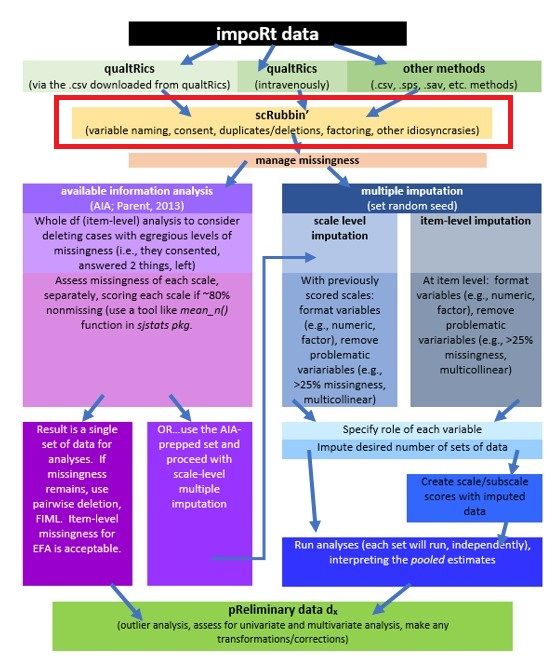
\includegraphics{images/Ch02/wrkflow_prelim.jpg}
\caption{An image of our stage in the workflow for scrubbing and scoring data.}
\end{figure}

\hypertarget{research-vignette-1}{%
\section{Research Vignette}\label{research-vignette-1}}

The research vignette comes from the survey titled, \href{https://spupsych.az1.qualtrics.com/jfe/form/SV_b2cClqAlLGQ6nLU}{Rate-a-Recent-Course: A ReCentering Psych Stats Exercise} and is explained in the prior chapter. In the prior chapter we conducted super-preliminary scrubbing of variables that will allow us to examine the respondent's perceived campus climate for students who are Black, predicted by the the respondent's own campus belonging, and also the \emph{structural diversity} proportions of Black students in the classroom and the BIPOC instructional staff. At present, I see this as a parallel mediation. That is, the perceived campus climate for Black students will be predicted by the respondent's sense of belonging, through the proportion of Black classmates and BIPOC (Black, Indigenous, and people of color)instructional staff.

\emph{I would like to assess the model by having the instructional staff variable to be the percent of Black instructional staff. At the time that this lecture is being prepared, there is insufficient representation of Black faculty to model this.}

\begin{figure}
\centering
\includegraphics{images/Ch03/BlStuMed.jpg}
\caption{An image of the statistical model for which we are preparing data.}
\end{figure}

First, though, let's take a more conceptual look at issues regarding missing data. We'll come back to details of the survey as we work with it.

\hypertarget{on-missing-data}{%
\section{On Missing Data}\label{on-missing-data}}

On the topic of missing data, we follow the traditions in most textbooks. We start by considering \emph{data loss mechanisms} and options for \emph{managing missingness.}

Although the workflow I recommend is fairly straightforward, the topic is not. Quantitative psychologist have produced volumes of research that supports and refutes all of these issues in detail. An in-deth review of this is found in Enders' \citeyearpar{enders_applied_2010} text.

\hypertarget{data-loss-mechanisms}{%
\subsection{Data Loss Mechanisms}\label{data-loss-mechanisms}}

We generally classify missingess in data in three different ways \citep{kline_principles_2016, parent_handling_2013}:

\textbf{Missing completely at random (MCAR)} is the ideal case (and often unrealistic in actual data). For variable \emph{Y} this mean that

\begin{itemize}
\tightlist
\item
  Missingness is due to a factor(s) completely unrelated to the missing data. Stated another way:

  \begin{itemize}
  \tightlist
  \item
    Missing observations differ from the observed scores only by chance; that is, whether scores on Y are missing or not missing is unrelated to \emph{Y} itself
  \end{itemize}
\item
  The presence versus absence of data on \emph{Y} is unrelated to all other variables in the dataset. That is, the nonmissing data are just a random sample of scores that the researcher would have analyzed had the data been complete. We might think of it as \emph{haphazard} missing.

  \begin{itemize}
  \tightlist
  \item
    A respondent is interrupted, looks up, looks down, and skips an item.
  \item
    A computer glitch causes spotty missingness -- unrelated to any particular variable.
  \end{itemize}
\end{itemize}

MCAR is the ideal state because results from it should not be biased as a function of the missingness.

\textbf{Missing at random (MAR)} missing data arise from a process that is both measured and predictable in a particular sample. \emph{Admittedly the use of ``random'' in this term is odd, because, by definition, the missingness is not random.}

Restated:

\begin{enumerate}
\def\labelenumi{\arabic{enumi}.}
\tightlist
\item
  Missingness on Y is unrelated to Y itself, but
\item
  Missingness is on Y is correlated with other variables in the data set.
\end{enumerate}

Example: Men are less likely to respond to questions about mental health than women, but among men, the probability of responding is unrelated to their true mental health status.

Kline \citeyearpar{kline_principles_2016} indicated that information loss due to MAR is potentially recoverable through imputation where missing scores are replaced by predicted scores. The predicted scores are generated from other variables in the data set that predict missingness on Y. If the strength of that prediction is reasonably strong, then results on Y after imputation may be relatively unbiased. In this sense, the MAR pattern is described as \emph{ignorable} with regard to potential bias. Two types of variables can be used to predict the missing data

\begin{enumerate}
\def\labelenumi{\arabic{enumi}.}
\tightlist
\item
  variables that are in the prediction equation, and
\item
  \emph{auxiliary} variables (i.e., variables in the dataset that are not in the prediction equation).
\end{enumerate}

Parent \citeyearpar{parent_handling_2013} noted that multiple imputation and expectation maximization have frequently been used to manage missingness in MAR circumstances.

\textbf{Missing not at random (MNAR)} is when the presence versus absence of scores on \emph{Y} depend on \emph{Y} itself. This is \emph{non-ignorable}.

For example, if a patient drops out of a medical RCT because there are unpleasant side effects from the treatment, this discomfort is not measured, but the data is missing due to a process that is unknown in a particular data set. Results based on \emph{complete cases only} can be severely biased when the data loss pattern is MNAR. That is, a treatment may look more beneficial than it really is if data from patients who were unable to tolerate the treatment are lost.

Parent \citeyearpar{parent_handling_2013} described MNAR a little differently -- but emphasized that the systematic missingness would be related to a variable outside the datset. Parent provided the example of items written in a manner that may be inappropriate for some participants (e.g., asking women about a relationship with their boyfriend/husband, when the woman might be in same gender relationship). If there were not demographic items that could identify the bias, this would be MNAR. Parent strongly advises researchers to carefully proofread and pilot surveys to avoid MNAR circumstances.

Kline \citeyearpar{kline_principles_2016} noted that the choice of the method to deal with the incomplete records can make a difference in the results, and should be made carefully.

\hypertarget{diagnosing-missing-data-mechanisms}{%
\subsection{Diagnosing Missing Data Mechanisms}\label{diagnosing-missing-data-mechanisms}}

The bad news is that we never really know (with certainty) the type of missing data mechanism in our data. The following tools can help understand the mechanisms that contribute to missingness.

\begin{itemize}
\tightlist
\item
  Missing data analyses often includes correlations that could predict missingness.
\item
  Little and Rubin \citeyearpar{little_statistical_2002} proposed a multivariate statistical test of the MCAR assumption that simultaneously compares complete versus incomplete cases on \emph{Y} across all other variables. If this comparison is significant, then the MCAR hypothesis is rejected.

  \begin{itemize}
  \tightlist
  \item
    To restate: we want a non-significant result; and we use the sometimes-backwards-sounding NHST (null hypothesis significance testing) language, ``MCAR cannot be rejected.''
  \end{itemize}
\item
  MCAR can also be examined through a series of \emph{t} tests of the cases that have missing scores on Y with cases that have complete records on other variables. Unfortunately, sample sizes contribute to problems with interpretation. With low samples, they are underpowered; in large samples they can flag trivial differences.
\end{itemize}

If MCAR is rejected, we are never sure whether the data loss mechanism is MAR or MNAR. There is no magical statistical ``fix.'' Kline \citeyearpar{kline_principles_2016} wrote, ``About the best that can be done is to understand the nature of the underlying data loss pattern and accordingly modify your interpretation of the results'' (p.~85).

\hypertarget{managing-missing-data}{%
\subsection{Managing Missing Data}\label{managing-missing-data}}

There are a number of approaches to managing missing data. Here is a summary of the ones most commonly used.

\begin{itemize}
\item
  \textbf{Listwise deletion} (aka, Complete Case Analysis) If there is a missing score on any variable, that case is excluded from \textbf{all} analyses.
\item
  \textbf{Pairwise deletion} Cases are excluded only if they have missing data on variables involved in a particular analysis. AIA is a variant of pair-wise deletion, but it preserves as much data as possible with person-mean imputation at the scale level.
\item
  \textbf{Mean/median substitution} Mean/median substitution replaces missing values with the mean/median of that particular variable. While this preserves the mean of the dataset, it can cause bias by decreasing variance. For example, if you have a column that has substantial of missingness and you replace each value with the same, fixed, mean, the variability of that variable has just been reduced. A variation on this is a \textbf{group-mean substitution} where the missing score in a particular group (e.g., women) is replaced by the group mean.
\item
  \textbf{Full information maximum likelihood (FIML)} A \emph{model-based method} that takes the researcher's model as the starting point. The procedure partitions the cases in a raw data file into subsets, each with the same pattern of missing observations, including none (complete cases). Statistical information (e.g., means, variances) is extracted from each subset so all case are retained in the analysis. Parameters for the researcher's model are estimated after combining all available information over the subsets of cases.
\item
  \textbf{Multiple imputation} A \emph{data based method} that works with the whole raw data file (not just with the observed variables that comprise the researcher's model). Multiple imputation assumes that data are MAR (remember, MCAR is the more prestigious one). This means that researchers assume that missing values can be replaced by predictions derived from the observable portion fo the dataset.

  \begin{itemize}
  \tightlist
  \item
    Multiple datasets (often 5 to 20) are created where missing values are replaced via a randomized process (so the same missing value {[}item 4 for person A{]} will likely have different values for each dataset).
  \item
    The desired anlayis(es) is conducted simultaneously/separately for each of the imputed sets (so if you imputed 5 sets and wanted a linear regression, you get 5 linear regressions).
  \item
    A \emph{pooled analysis} uses the point estimates and the standard errors to provide a single result that represents the analysis.
  \end{itemize}
\end{itemize}

\hypertarget{available-information-analysis-aia}{%
\subsection{Available Information Analysis (AIA)}\label{available-information-analysis-aia}}

Parent \citeyearpar{parent_handling_2013} has created a set of recommendations that help us create a streamlined workflow for managing missing data. After evaluating three approaches to managing missingness (AIA, mean substitution, and multiple imputation) Parent concluded that in datasets with (a) low levels of missingness, (b) a reasonable sample size, and (c) adequate internal reliability of measures, these approaches had similar results.

Further, in simulation studies where there was (a) low sample size (\emph{n} = 50), (b) weak associations among items, and (c) a small number of missing items, AIA was equivalent to multiple imputation. Even in cases where the data conditions were the ``best'' (i.e., \emph{N} = 200, moderate correlations, at least 10 items), even 10\% missingness (overall) did not produce notable difference among the methods. That is, means, standard errors, and alphas were similar across the methods (AIA, mean substitution, multiple imputation).

AIA is an older method of handling missing data that, as its name suggests, uses the \emph{available data} for analysis and excludes missing data points only for analyses in which the missing data point would be directly involved. This means

\begin{itemize}
\tightlist
\item
  In the case of research that uses multiple item scales, and analysis takes place at the scale level

  \begin{itemize}
  \tightlist
  \item
    AIA is used to generate \textbf{mean} scores for the scale using the available data without substituting or imputing values;
  \item
    This method generally produces a fairly complete set of scale-level data where

    \begin{itemize}
    \tightlist
    \item
      pairwise deletion (the whole row/case/person is skipped) can be used where there will be multiple analyses using statistics (e.g., correlations, t-tests, ANOVA) were missingness is not permitted
    \item
      FIML can be specified in path analysis and CFA/SEM (where item-level data is required), and
    \item
      some statistics, such as principal components analysis and principal axis factoring (item-level analyses) permit missing data,
    \end{itemize}
  \item
    Of course, the researcher could still impute data, but why\ldots{}
  \end{itemize}
\end{itemize}

Parent's \citeyearpar{parent_handling_2013} recommendations:

\begin{itemize}
\tightlist
\item
  Scale scores should be first calculated as a \emph{mean} (average) not a sum. Why?

  \begin{itemize}
  \tightlist
  \item
    Calculating a ``sum'' from available data will result in automatically lower scores in cases where there is missingness.
  \item
    If a sum is required (i.e., because you want to interpret some clinical level of something), calculate the mean first, do the analyses, then transform the results back into the whole-scale equivalent (multiply the mean by the number of items) for any interpretation.
  \item
    For R script, do not write the script ({[}item1 + item2 + item3{]}/3) because this will return an empty entry for participants missing data (same problem as if you were to use sum). There are several functions for properly computing a mean; I will demo the \emph{mean\_n()} function from \emph{sjstats} package because it allows us to simultaneously specify the tolerance level (next item).
  \end{itemize}
\item
  Determine your \emph{tolerance} for missingness (20\% seems to be common, although you could also look for guidance in the test manual/article). Then

  \begin{itemize}
  \tightlist
  \item
    Run a ``percent missingness'' check on the level of analysis (i.e., total score, scale, or subscale) you are using. If you are using a total scale score, then check to see what percent is missing across all the items in the whole scale. In contrast, if you are looking at subscales, run the percent missing at that level.
  \item
    Parent \citeyearpar{parent_handling_2013} advised that the tolerance levels should be made mindfully. A four-item scale with one item missing, won't meet the 80\% threshold, so it may make sense to set a 75\% threshold for this scale.
  \end{itemize}
\item
  ``Clearly and concisely detail the level of missingness'' in papers \citep[p.~595]{parent_handling_2013}. This includes

  \begin{itemize}
  \tightlist
  \item
    tolerance level for missing data by scale or subscale (e.g., 80\% or 75\%)
  \item
    the number of missing values out of all data points on that scale for all participants and the maximum by participant (e.g., ``For Scale X, a total of \# missing data points out of \#\#\# were observed with no participant missing more than a single point.'')
  \item
    verify a manual inspection of missing data for obvious patterns (e.g., abnormally high missing rates for only one or two items). This can be accomplished by requesting frequency output for the items and checking the nonmissing data points for each scale, ensuring there are no abnormal spikes in missingness (looking for MNAR).
  \end{itemize}
\item
  Curiously, Parent \citeyearpar{parent_handling_2013} does not recommend that we run all the diagnostic tests. However, because recent reviewers have required them of me, I will demonstrate a series of them.
\item
  Reducing missingness starts at the survey design -- make sure that all people can answer all items (i.e,. relationship-related items may contain heterosexist assumptions\ldots which would result in an MNAR circumstance)
\end{itemize}

Very practically speaking, Parent's \citeyearpar{parent_handling_2013} recommendations follow us through the entire data analysis process.

\hypertarget{working-the-problem-1}{%
\section{Working the Problem}\label{working-the-problem-1}}

\hypertarget{variable-planning-and-preparation}{%
\subsection{Variable Planning and Preparation}\label{variable-planning-and-preparation}}

In the \protect\hyperlink{scrub}{Scrubbing lesson} we imported the data from Qualtrics and applied the broadest levels of inclusion (e.g., the course rated was offered from an institution in the U.S., the respondent consented to participation) and exclusion (e.g., the survey was not a preview). We then downsized the survey to include the variables we will use in our statistical model. We then saved the data in .csv and .rds file.

Presuming that you are working along with me in an .rmd file and have placed that file in the same folder as this .rmd file, the following code should read the data into your environment.

I use \emph{different} names for the object/df in my R environment than I use for the filename that holds the data on my computer. Why? I don't want to accidentally overwrite this precious ``source'' of data.

\begin{Shaded}
\begin{Highlighting}[]
\CommentTok{\# scrub\_df \textless{}{-} read.csv (\textquotesingle{}BlackStntsModel230902.csv\textquotesingle{}, head = TRUE, sep}
\CommentTok{\# = \textquotesingle{},\textquotesingle{})}
\NormalTok{scrub\_df }\OtherTok{\textless{}{-}} \FunctionTok{readRDS}\NormalTok{(}\StringTok{"BlackStntsModel230902.rds"}\NormalTok{)}
\FunctionTok{str}\NormalTok{(scrub\_df)}
\end{Highlighting}
\end{Shaded}

\begin{verbatim}
## Classes 'tbl_df', 'tbl' and 'data.frame':    69 obs. of  25 variables:
##  $ ID       : int  1 2 3 4 5 6 7 8 9 10 ...
##  $ iRace1   : num  3 3 3 3 1 3 3 3 1 0 ...
##   ..- attr(*, "label")= Named chr "1 - From your perspective as a student, which of the following best describes the [Field-2] instructor."
##   .. ..- attr(*, "names")= chr "1_iRace"
##  $ iRace2   : num  1 NA 1 1 NA NA 3 NA NA 0 ...
##   ..- attr(*, "label")= Named chr "2 - From your perspective as a student, which of the following best describes the [Field-2] instructor."
##   .. ..- attr(*, "names")= chr "2_iRace"
##  $ iRace3   : num  3 NA NA 3 NA NA NA NA NA 3 ...
##   ..- attr(*, "label")= Named chr "3 - From your perspective as a student, which of the following best describes the [Field-2] instructor."
##   .. ..- attr(*, "names")= chr "3_iRace"
##  $ iRace4   : num  NA NA NA NA NA NA NA NA NA 3 ...
##   ..- attr(*, "label")= Named chr "4 - From your perspective as a student, which of the following best describes the [Field-2] instructor."
##   .. ..- attr(*, "names")= chr "4_iRace"
##  $ iRace5   : logi  NA NA NA NA NA NA ...
##   ..- attr(*, "label")= Named chr "5 - From your perspective as a student, which of the following best describes the [Field-2] instructor."
##   .. ..- attr(*, "names")= chr "5_iRace"
##  $ iRace6   : logi  NA NA NA NA NA NA ...
##   ..- attr(*, "label")= Named chr "6 - From your perspective as a student, which of the following best describes the [Field-2] instructor."
##   .. ..- attr(*, "names")= chr "6_iRace"
##  $ iRace7   : logi  NA NA NA NA NA NA ...
##   ..- attr(*, "label")= Named chr "7 - From your perspective as a student, which of the following best describes the [Field-2] instructor."
##   .. ..- attr(*, "names")= chr "7_iRace"
##  $ iRace8   : logi  NA NA NA NA NA NA ...
##   ..- attr(*, "label")= Named chr "8 - From your perspective as a student, which of the following best describes the [Field-2] instructor."
##   .. ..- attr(*, "names")= chr "8_iRace"
##  $ iRace9   : logi  NA NA NA NA NA NA ...
##   ..- attr(*, "label")= Named chr "9 - From your perspective as a student, which of the following best describes the [Field-2] instructor."
##   .. ..- attr(*, "names")= chr "9_iRace"
##  $ iRace10  : logi  NA NA NA NA NA NA ...
##   ..- attr(*, "label")= Named chr "10 - From your perspective as a student, which of the following best describes the [Field-2] instructor."
##   .. ..- attr(*, "names")= chr "10_iRace"
##  $ cmBiMulti: num  0 0 0 2 5 15 0 0 0 7 ...
##   ..- attr(*, "label")= Named chr "Regarding race, what proportion of students were from each broad classification.  Your responses should add to "| __truncated__
##   .. ..- attr(*, "names")= chr "Race_10"
##  $ cmBlack  : num  0 5 10 6 5 20 0 0 0 4 ...
##   ..- attr(*, "label")= Named chr "Regarding race, what proportion of students were from each broad classification.  Your responses should add to 100%. - Black"
##   .. ..- attr(*, "names")= chr "Race_1"
##  $ cmNBPoC  : num  39 10 30 19 10 30 40 5 30 13 ...
##   ..- attr(*, "label")= Named chr "Regarding race, what proportion of students were from each broad classification.  Your responses should add to "| __truncated__
##   .. ..- attr(*, "names")= chr "Race_7"
##  $ cmWhite  : num  61 85 60 73 80 35 60 90 70 73 ...
##   ..- attr(*, "label")= Named chr "Regarding race, what proportion of students were from each broad classification.  Your responses should add to 100%. - White"
##   .. ..- attr(*, "names")= chr "Race_8"
##  $ cmUnsure : num  0 0 0 0 0 0 0 5 0 3 ...
##   ..- attr(*, "label")= Named chr "Regarding race, what proportion of students were from each broad classification.  Your responses should add to 100%. - Unsure"
##   .. ..- attr(*, "names")= chr "Race_2"
##  $ Belong_1 : num  6 4 NA 5 4 5 6 7 6 3 ...
##   ..- attr(*, "label")= Named chr "Please indicate the degree to which you agree with the following questions about the course. Please skip the it"| __truncated__
##   .. ..- attr(*, "names")= chr "Belong_1"
##  $ Belong_2 : num  6 4 3 3 4 6 6 7 6 3 ...
##   ..- attr(*, "label")= Named chr "Please indicate the degree to which you agree with the following questions about the course. Please skip the it"| __truncated__
##   .. ..- attr(*, "names")= chr "Belong_2"
##  $ Belong_3 : num  7 6 NA 2 4 5 5 7 6 3 ...
##   ..- attr(*, "label")= Named chr "Please indicate the degree to which you agree with the following questions about the course. Please skip the it"| __truncated__
##   .. ..- attr(*, "names")= chr "Belong_3"
##  $ Blst_1   : num  5 6 NA 2 6 5 5 5 5 3 ...
##   ..- attr(*, "label")= Named chr "Each item below asks you to rate elements of campus climate for your \"academic department/program.\"  If you d"| __truncated__
##   .. ..- attr(*, "names")= chr "Blst_1"
##  $ Blst_2   : num  3 6 5 2 1 1 4 4 3 5 ...
##   ..- attr(*, "label")= Named chr "Each item below asks you to rate elements of campus climate for your \"academic department/program.\"  If you d"| __truncated__
##   .. ..- attr(*, "names")= chr "Blst_2"
##  $ Blst_3   : num  5 2 2 2 1 1 4 3 1 2 ...
##   ..- attr(*, "label")= Named chr "Each item below asks you to rate elements of campus climate for your \"academic department/program.\"  If you d"| __truncated__
##   .. ..- attr(*, "names")= chr "Blst_3"
##  $ Blst_4   : num  2 2 2 2 1 2 4 3 2 3 ...
##   ..- attr(*, "label")= Named chr "Each item below asks you to rate elements of campus climate for your \"academic department/program.\"  If you d"| __truncated__
##   .. ..- attr(*, "names")= chr "Blst_4"
##  $ Blst_5   : num  2 4 NA 2 1 1 4 4 1 3 ...
##   ..- attr(*, "label")= Named chr "Each item below asks you to rate elements of campus climate for your \"academic department/program.\"  If you d"| __truncated__
##   .. ..- attr(*, "names")= chr "Blst_5"
##  $ Blst_6   : num  2 1 2 2 1 2 4 3 2 3 ...
##   ..- attr(*, "label")= Named chr "Each item below asks you to rate elements of campus climate for your \"academic department/program.\"  If you d"| __truncated__
##   .. ..- attr(*, "names")= chr "Blst_6"
##  - attr(*, "column_map")=Classes 'tbl_df', 'tbl' and 'data.frame':   182 obs. of  7 variables:
##   ..$ qname      : chr [1:182] "StartDate" "EndDate" "Status" "Progress" ...
##   ..$ description: chr [1:182] "Start Date" "End Date" "Response Type" "Progress" ...
##   ..$ main       : chr [1:182] "Start Date" "End Date" "Response Type" "Progress" ...
##   ..$ sub        : chr [1:182] "" "" "" "" ...
##   ..$ ImportId   : chr [1:182] "startDate" "endDate" "status" "progress" ...
##   ..$ timeZone   : chr [1:182] "America/Los_Angeles" "America/Los_Angeles" NA NA ...
##   ..$ choiceId   : chr [1:182] NA NA NA NA ...
\end{verbatim}

Let's think about how the variables in our model should be measured:

\begin{itemize}
\tightlist
\item
  DV: Campus Climate for Black Students (as perceived by the respondent)

  \begin{itemize}
  \tightlist
  \item
    mean score of the 6 items on that scale (higher scores indicate a climate characterized by hostility, nonresponsiveness, and stigma)
  \item
    1 item needs to be reverse-coded
  \item
    this scale was adapted from the LGBT Campus Climate Scale \citep{szymanski_perceptions_2020}
  \end{itemize}
\item
  IV: Belonging

  \begin{itemize}
  \tightlist
  \item
    mean score for the 3 items on that scale (higher scores indicate a greater sense of belonging)
  \item
    this scale is taken from the Sense of Belonging subscale from the Perceived Cohesion Scale \citep{bollen_perceived_1990}
  \end{itemize}
\item
  Proportion of classmates who are Black

  \begin{itemize}
  \tightlist
  \item
    a single item
  \end{itemize}
\item
  Proportion of instructional staff who are BIPOC

  \begin{itemize}
  \tightlist
  \item
    must be calculated from each of the single items for each instructor
  \end{itemize}
\end{itemize}

To summarize, the Campus Climate and Belonging scales are traditional in the sense that they have items that we sum. The variable representing proportion of classmates who are Black is a single item. The variable representing the proportion of instructional staff who are BIPOC must be calculated in a manner that takes into consideration the there may be multiple instructors. The survey allowed a respondent to name up to 10 instructors.

\begin{Shaded}
\begin{Highlighting}[]
\FunctionTok{str}\NormalTok{(scrub\_df}\SpecialCharTok{$}\NormalTok{iRace1)}
\end{Highlighting}
\end{Shaded}

\begin{verbatim}
##  num [1:69] 3 3 3 3 1 3 3 3 1 0 ...
##  - attr(*, "label")= Named chr "1 - From your perspective as a student, which of the following best describes the [Field-2] instructor."
##   ..- attr(*, "names")= chr "1_iRace"
\end{verbatim}

Looking at the structure of our data, the iRace(1 thru 10) variables are in ``int'' or integer format. This means that they are represented as whole numbers. We need them to be represented as factors. R handles factors represented as words well. Therefore, let's use our codebook to reformat this variable as a an ordered factor, with words instead of numbers.

Qualtrics imports many of the categorical variables as numbers. R often reads them numerically (integers or numbers). If they are directly converted to factors, R will sometimes collapse across missing numbers. In this example, if there is a race that is not represented (e.g., 2 for BiMulti), when the numbers are changed to factors, R will assume they are ordered and there is a consecutive series of numbers (0,1,2,3,4). If a number in the sequence is missing (0,1,3,4) and labels are applied, it will collapse across the numbers and the labels you think are attached to each number are not. Therefore, it is ESSENTIAL to check (again and again ad nauseum) to ensure that your variables are recoding in a manner you understand.

One way to avoid this is to use the code below to identify the levels and the labels. When they are in order, they align and don't ``skip'' numbers. To quadruple check our work, we will recode into a new variable ``tRace\#'' for ``teacher'' Race.

\begin{Shaded}
\begin{Highlighting}[]
\NormalTok{scrub\_df}\SpecialCharTok{$}\NormalTok{tRace1 }\OtherTok{=} \FunctionTok{factor}\NormalTok{(scrub\_df}\SpecialCharTok{$}\NormalTok{iRace1, }\AttributeTok{levels =} \FunctionTok{c}\NormalTok{(}\DecValTok{0}\NormalTok{, }\DecValTok{1}\NormalTok{, }\DecValTok{2}\NormalTok{, }\DecValTok{3}\NormalTok{, }\DecValTok{4}\NormalTok{), }\AttributeTok{labels =} \FunctionTok{c}\NormalTok{(}\StringTok{"Black"}\NormalTok{,}
    \StringTok{"nBpoc"}\NormalTok{, }\StringTok{"BiMulti"}\NormalTok{, }\StringTok{"White"}\NormalTok{, }\StringTok{"NotNotice"}\NormalTok{))}
\NormalTok{scrub\_df}\SpecialCharTok{$}\NormalTok{tRace2 }\OtherTok{=} \FunctionTok{factor}\NormalTok{(scrub\_df}\SpecialCharTok{$}\NormalTok{iRace2, }\AttributeTok{levels =} \FunctionTok{c}\NormalTok{(}\DecValTok{0}\NormalTok{, }\DecValTok{1}\NormalTok{, }\DecValTok{2}\NormalTok{, }\DecValTok{3}\NormalTok{, }\DecValTok{4}\NormalTok{), }\AttributeTok{labels =} \FunctionTok{c}\NormalTok{(}\StringTok{"Black"}\NormalTok{,}
    \StringTok{"nBpoc"}\NormalTok{, }\StringTok{"BiMulti"}\NormalTok{, }\StringTok{"White"}\NormalTok{, }\StringTok{"NotNotice"}\NormalTok{))}
\NormalTok{scrub\_df}\SpecialCharTok{$}\NormalTok{tRace3 }\OtherTok{=} \FunctionTok{factor}\NormalTok{(scrub\_df}\SpecialCharTok{$}\NormalTok{iRace3, }\AttributeTok{levels =} \FunctionTok{c}\NormalTok{(}\DecValTok{0}\NormalTok{, }\DecValTok{1}\NormalTok{, }\DecValTok{2}\NormalTok{, }\DecValTok{3}\NormalTok{, }\DecValTok{4}\NormalTok{), }\AttributeTok{labels =} \FunctionTok{c}\NormalTok{(}\StringTok{"Black"}\NormalTok{,}
    \StringTok{"nBpoc"}\NormalTok{, }\StringTok{"BiMulti"}\NormalTok{, }\StringTok{"White"}\NormalTok{, }\StringTok{"NotNotice"}\NormalTok{))}
\NormalTok{scrub\_df}\SpecialCharTok{$}\NormalTok{tRace4 }\OtherTok{=} \FunctionTok{factor}\NormalTok{(scrub\_df}\SpecialCharTok{$}\NormalTok{iRace4, }\AttributeTok{levels =} \FunctionTok{c}\NormalTok{(}\DecValTok{0}\NormalTok{, }\DecValTok{1}\NormalTok{, }\DecValTok{2}\NormalTok{, }\DecValTok{3}\NormalTok{, }\DecValTok{4}\NormalTok{), }\AttributeTok{labels =} \FunctionTok{c}\NormalTok{(}\StringTok{"Black"}\NormalTok{,}
    \StringTok{"nBpoc"}\NormalTok{, }\StringTok{"BiMulti"}\NormalTok{, }\StringTok{"White"}\NormalTok{, }\StringTok{"NotNotice"}\NormalTok{))}
\NormalTok{scrub\_df}\SpecialCharTok{$}\NormalTok{tRace5 }\OtherTok{=} \FunctionTok{factor}\NormalTok{(scrub\_df}\SpecialCharTok{$}\NormalTok{iRace5, }\AttributeTok{levels =} \FunctionTok{c}\NormalTok{(}\DecValTok{0}\NormalTok{, }\DecValTok{1}\NormalTok{, }\DecValTok{2}\NormalTok{, }\DecValTok{3}\NormalTok{, }\DecValTok{4}\NormalTok{), }\AttributeTok{labels =} \FunctionTok{c}\NormalTok{(}\StringTok{"Black"}\NormalTok{,}
    \StringTok{"nBpoc"}\NormalTok{, }\StringTok{"BiMulti"}\NormalTok{, }\StringTok{"White"}\NormalTok{, }\StringTok{"NotNotice"}\NormalTok{))}
\NormalTok{scrub\_df}\SpecialCharTok{$}\NormalTok{tRace6 }\OtherTok{=} \FunctionTok{factor}\NormalTok{(scrub\_df}\SpecialCharTok{$}\NormalTok{iRace6, }\AttributeTok{levels =} \FunctionTok{c}\NormalTok{(}\DecValTok{0}\NormalTok{, }\DecValTok{1}\NormalTok{, }\DecValTok{2}\NormalTok{, }\DecValTok{3}\NormalTok{, }\DecValTok{4}\NormalTok{), }\AttributeTok{labels =} \FunctionTok{c}\NormalTok{(}\StringTok{"Black"}\NormalTok{,}
    \StringTok{"nBpoc"}\NormalTok{, }\StringTok{"BiMulti"}\NormalTok{, }\StringTok{"White"}\NormalTok{, }\StringTok{"NotNotice"}\NormalTok{))}
\NormalTok{scrub\_df}\SpecialCharTok{$}\NormalTok{tRace7 }\OtherTok{=} \FunctionTok{factor}\NormalTok{(scrub\_df}\SpecialCharTok{$}\NormalTok{iRace7, }\AttributeTok{levels =} \FunctionTok{c}\NormalTok{(}\DecValTok{0}\NormalTok{, }\DecValTok{1}\NormalTok{, }\DecValTok{2}\NormalTok{, }\DecValTok{3}\NormalTok{, }\DecValTok{4}\NormalTok{), }\AttributeTok{labels =} \FunctionTok{c}\NormalTok{(}\StringTok{"Black"}\NormalTok{,}
    \StringTok{"nBpoc"}\NormalTok{, }\StringTok{"BiMulti"}\NormalTok{, }\StringTok{"White"}\NormalTok{, }\StringTok{"NotNotice"}\NormalTok{))}
\NormalTok{scrub\_df}\SpecialCharTok{$}\NormalTok{tRace8 }\OtherTok{=} \FunctionTok{factor}\NormalTok{(scrub\_df}\SpecialCharTok{$}\NormalTok{iRace8, }\AttributeTok{levels =} \FunctionTok{c}\NormalTok{(}\DecValTok{0}\NormalTok{, }\DecValTok{1}\NormalTok{, }\DecValTok{2}\NormalTok{, }\DecValTok{3}\NormalTok{, }\DecValTok{4}\NormalTok{), }\AttributeTok{labels =} \FunctionTok{c}\NormalTok{(}\StringTok{"Black"}\NormalTok{,}
    \StringTok{"nBpoc"}\NormalTok{, }\StringTok{"BiMulti"}\NormalTok{, }\StringTok{"White"}\NormalTok{, }\StringTok{"NotNotice"}\NormalTok{))}
\NormalTok{scrub\_df}\SpecialCharTok{$}\NormalTok{tRace9 }\OtherTok{=} \FunctionTok{factor}\NormalTok{(scrub\_df}\SpecialCharTok{$}\NormalTok{iRace9, }\AttributeTok{levels =} \FunctionTok{c}\NormalTok{(}\DecValTok{0}\NormalTok{, }\DecValTok{1}\NormalTok{, }\DecValTok{2}\NormalTok{, }\DecValTok{3}\NormalTok{, }\DecValTok{4}\NormalTok{), }\AttributeTok{labels =} \FunctionTok{c}\NormalTok{(}\StringTok{"Black"}\NormalTok{,}
    \StringTok{"nBpoc"}\NormalTok{, }\StringTok{"BiMulti"}\NormalTok{, }\StringTok{"White"}\NormalTok{, }\StringTok{"NotNotice"}\NormalTok{))}
\NormalTok{scrub\_df}\SpecialCharTok{$}\NormalTok{tRace10 }\OtherTok{=} \FunctionTok{factor}\NormalTok{(scrub\_df}\SpecialCharTok{$}\NormalTok{iRace10, }\AttributeTok{levels =} \FunctionTok{c}\NormalTok{(}\DecValTok{0}\NormalTok{, }\DecValTok{1}\NormalTok{, }\DecValTok{2}\NormalTok{, }\DecValTok{3}\NormalTok{, }\DecValTok{4}\NormalTok{),}
    \AttributeTok{labels =} \FunctionTok{c}\NormalTok{(}\StringTok{"Black"}\NormalTok{, }\StringTok{"nBpoc"}\NormalTok{, }\StringTok{"BiMulti"}\NormalTok{, }\StringTok{"White"}\NormalTok{, }\StringTok{"NotNotice"}\NormalTok{))}
\end{Highlighting}
\end{Shaded}

Let's check the structure to see if they are factors.

\begin{Shaded}
\begin{Highlighting}[]
\FunctionTok{library}\NormalTok{(tidyverse)}
\end{Highlighting}
\end{Shaded}

\begin{verbatim}
## -- Attaching core tidyverse packages ------------------------ tidyverse 2.0.0 --
## v dplyr     1.1.2     v readr     2.1.4
## v forcats   1.0.0     v stringr   1.5.0
## v ggplot2   3.4.3     v tibble    3.2.1
## v lubridate 1.9.2     v tidyr     1.3.0
## v purrr     1.0.1     
## -- Conflicts ------------------------------------------ tidyverse_conflicts() --
## x dplyr::filter() masks stats::filter()
## x dplyr::lag()    masks stats::lag()
## i Use the conflicted package (<http://conflicted.r-lib.org/>) to force all conflicts to become errors
\end{verbatim}

\begin{Shaded}
\begin{Highlighting}[]
\FunctionTok{glimpse}\NormalTok{(scrub\_df)}
\end{Highlighting}
\end{Shaded}

\begin{verbatim}
## Rows: 69
## Columns: 35
## $ ID        <int> 1, 2, 3, 4, 5, 6, 7, 8, 9, 10, 11, 12, 13, 14, 15, 16, 17, 1~
## $ iRace1    <dbl> 3, 3, 3, 3, 1, 3, 3, 3, 1, 0, 2, 1, 1, 1, 3, 3, 3, 1, 3, 3, ~
## $ iRace2    <dbl> 1, NA, 1, 1, NA, NA, 3, NA, NA, 0, NA, NA, 3, NA, 3, 3, NA, ~
## $ iRace3    <dbl> 3, NA, NA, 3, NA, NA, NA, NA, NA, 3, NA, NA, NA, NA, 3, 1, N~
## $ iRace4    <dbl> NA, NA, NA, NA, NA, NA, NA, NA, NA, 3, NA, NA, NA, NA, NA, 3~
## $ iRace5    <lgl> NA, NA, NA, NA, NA, NA, NA, NA, NA, NA, NA, NA, NA, NA, NA, ~
## $ iRace6    <lgl> NA, NA, NA, NA, NA, NA, NA, NA, NA, NA, NA, NA, NA, NA, NA, ~
## $ iRace7    <lgl> NA, NA, NA, NA, NA, NA, NA, NA, NA, NA, NA, NA, NA, NA, NA, ~
## $ iRace8    <lgl> NA, NA, NA, NA, NA, NA, NA, NA, NA, NA, NA, NA, NA, NA, NA, ~
## $ iRace9    <lgl> NA, NA, NA, NA, NA, NA, NA, NA, NA, NA, NA, NA, NA, NA, NA, ~
## $ iRace10   <lgl> NA, NA, NA, NA, NA, NA, NA, NA, NA, NA, NA, NA, NA, NA, NA, ~
## $ cmBiMulti <dbl> 0, 0, 0, 2, 5, 15, 0, 0, 0, 7, 0, 0, 20, 0, 9, 12, 0, 6, 6, ~
## $ cmBlack   <dbl> 0, 5, 10, 6, 5, 20, 0, 0, 0, 4, 0, 7, 0, 6, 9, 1, 21, 5, 6, ~
## $ cmNBPoC   <dbl> 39, 10, 30, 19, 10, 30, 40, 5, 30, 13, 80, 19, 0, 19, 15, 22~
## $ cmWhite   <dbl> 61, 85, 60, 73, 80, 35, 60, 90, 70, 73, 10, 74, 80, 0, 67, 5~
## $ cmUnsure  <dbl> 0, 0, 0, 0, 0, 0, 0, 5, 0, 3, 10, 0, 0, 75, 0, 14, 0, 5, 0, ~
## $ Belong_1  <dbl> 6, 4, NA, 5, 4, 5, 6, 7, 6, 3, 6, 6, 3, 4, 3, 3, 4, 5, 1, 2,~
## $ Belong_2  <dbl> 6, 4, 3, 3, 4, 6, 6, 7, 6, 3, 6, 6, 5, 4, 3, 3, 4, 6, 1, 2, ~
## $ Belong_3  <dbl> 7, 6, NA, 2, 4, 5, 5, 7, 6, 3, 5, 6, 4, 4, 3, 2, 4, 5, 1, 1,~
## $ Blst_1    <dbl> 5, 6, NA, 2, 6, 5, 5, 5, 5, 3, NA, 4, 5, 6, 3, 4, 6, 4, 4, 4~
## $ Blst_2    <dbl> 3, 6, 5, 2, 1, 1, 4, 4, 3, 5, NA, 5, 1, 1, 3, 2, 1, 2, 5, 3,~
## $ Blst_3    <dbl> 5, 2, 2, 2, 1, 1, 4, 3, 1, 2, 2, 1, 1, 1, 3, 2, 6, 2, 2, 2, ~
## $ Blst_4    <dbl> 2, 2, 2, 2, 1, 2, 4, 3, 2, 3, NA, 4, 3, 1, 3, 2, 1, 3, 2, 1,~
## $ Blst_5    <dbl> 2, 4, NA, 2, 1, 1, 4, 4, 1, 3, 2, 2, 1, 1, 3, 2, 1, 2, 2, 1,~
## $ Blst_6    <dbl> 2, 1, 2, 2, 1, 2, 4, 3, 2, 3, NA, 2, 1, 1, 3, 2, 2, 3, 2, 1,~
## $ tRace1    <fct> White, White, White, White, nBpoc, White, White, White, nBpo~
## $ tRace2    <fct> nBpoc, NA, nBpoc, nBpoc, NA, NA, White, NA, NA, Black, NA, N~
## $ tRace3    <fct> White, NA, NA, White, NA, NA, NA, NA, NA, White, NA, NA, NA,~
## $ tRace4    <fct> NA, NA, NA, NA, NA, NA, NA, NA, NA, White, NA, NA, NA, NA, N~
## $ tRace5    <fct> NA, NA, NA, NA, NA, NA, NA, NA, NA, NA, NA, NA, NA, NA, NA, ~
## $ tRace6    <fct> NA, NA, NA, NA, NA, NA, NA, NA, NA, NA, NA, NA, NA, NA, NA, ~
## $ tRace7    <fct> NA, NA, NA, NA, NA, NA, NA, NA, NA, NA, NA, NA, NA, NA, NA, ~
## $ tRace8    <fct> NA, NA, NA, NA, NA, NA, NA, NA, NA, NA, NA, NA, NA, NA, NA, ~
## $ tRace9    <fct> NA, NA, NA, NA, NA, NA, NA, NA, NA, NA, NA, NA, NA, NA, NA, ~
## $ tRace10   <fct> NA, NA, NA, NA, NA, NA, NA, NA, NA, NA, NA, NA, NA, NA, NA, ~
\end{verbatim}

Calculating the proportion of the BIPOC instructional staff could likely be accomplished a number of ways. My searching for solutions resulted in this. Hopefully it's a fair balance between intuitive and elegant coding. First, I created code that

\begin{itemize}
\tightlist
\item
  created a new variable (count.BIPOC) by

  \begin{itemize}
  \tightlist
  \item
    summing across the tRace1 through tRace10 variables,
  \item
    assigning a count of ``1'' each time the factor value was Black, nBpoc, or BiMulti
  \end{itemize}
\end{itemize}

\begin{Shaded}
\begin{Highlighting}[]
\NormalTok{scrub\_df}\SpecialCharTok{$}\NormalTok{count.BIPOC }\OtherTok{\textless{}{-}} \FunctionTok{apply}\NormalTok{(scrub\_df[}\FunctionTok{c}\NormalTok{(}\StringTok{"tRace1"}\NormalTok{, }\StringTok{"tRace2"}\NormalTok{, }\StringTok{"tRace3"}\NormalTok{,}
    \StringTok{"tRace4"}\NormalTok{, }\StringTok{"tRace5"}\NormalTok{, }\StringTok{"tRace6"}\NormalTok{, }\StringTok{"tRace7"}\NormalTok{, }\StringTok{"tRace8"}\NormalTok{, }\StringTok{"tRace9"}\NormalTok{, }\StringTok{"tRace10"}\NormalTok{)],}
    \DecValTok{1}\NormalTok{, }\ControlFlowTok{function}\NormalTok{(x) }\FunctionTok{sum}\NormalTok{(x }\SpecialCharTok{\%in\%} \FunctionTok{c}\NormalTok{(}\StringTok{"Black"}\NormalTok{, }\StringTok{"nBpoc"}\NormalTok{, }\StringTok{"BiMulti"}\NormalTok{)))}
\end{Highlighting}
\end{Shaded}

Next, I created a variable that counted the number of non-missing values across the tRace1 through tRace10 variables.

\begin{Shaded}
\begin{Highlighting}[]
\NormalTok{scrub\_df}\SpecialCharTok{$}\NormalTok{count.nMiss }\OtherTok{\textless{}{-}} \FunctionTok{apply}\NormalTok{(scrub\_df[}\FunctionTok{c}\NormalTok{(}\StringTok{"tRace1"}\NormalTok{, }\StringTok{"tRace2"}\NormalTok{, }\StringTok{"tRace3"}\NormalTok{,}
    \StringTok{"tRace4"}\NormalTok{, }\StringTok{"tRace5"}\NormalTok{, }\StringTok{"tRace6"}\NormalTok{, }\StringTok{"tRace7"}\NormalTok{, }\StringTok{"tRace8"}\NormalTok{, }\StringTok{"tRace9"}\NormalTok{, }\StringTok{"tRace10"}\NormalTok{)],}
    \DecValTok{1}\NormalTok{, }\ControlFlowTok{function}\NormalTok{(x) }\FunctionTok{sum}\NormalTok{(}\SpecialCharTok{!}\FunctionTok{is.na}\NormalTok{(x)))}
\end{Highlighting}
\end{Shaded}

Now to calculate the proportion of BIPOC instructional faculty for each case.

\begin{Shaded}
\begin{Highlighting}[]
\NormalTok{scrub\_df}\SpecialCharTok{$}\NormalTok{iBIPOC\_pr }\OtherTok{=}\NormalTok{ scrub\_df}\SpecialCharTok{$}\NormalTok{count.BIPOC}\SpecialCharTok{/}\NormalTok{scrub\_df}\SpecialCharTok{$}\NormalTok{count.nMiss}
\end{Highlighting}
\end{Shaded}

\hypertarget{missing-data-analysis-whole-df-and-item-level}{%
\subsection{Missing Data Analysis: Whole df and Item level}\label{missing-data-analysis-whole-df-and-item-level}}

In understanding missingness across the dataset, I think it is important to analyze and manage it, iteratively. We will start with a view of the whole df-level missingness. Subsequently, and consistent with the available information analysis {[}AIA; \citet{parent_handling_2013}{]} approach, we will score the scales and then look again at missingness, using the new information to update our decisions about how to manage it.

\begin{figure}
\centering
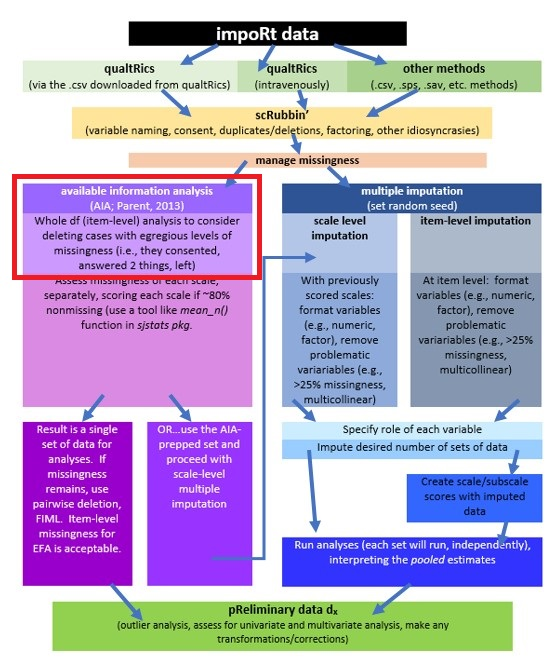
\includegraphics{images/Ch02/wrkflow_item_lvl.jpg}
\caption{An image of our stage in the workflow for scrubbing and scoring data.}
\end{figure}

Because we just created a host of new variables in creating the \emph{prop\_BIPOC} variable, let's downsize the df so that the calculations are sensible.

\begin{Shaded}
\begin{Highlighting}[]
\NormalTok{scrub\_df }\OtherTok{\textless{}{-}}\NormalTok{ (}\FunctionTok{select}\NormalTok{(scrub\_df, ID, iBIPOC\_pr, cmBlack, Belong\_1}\SpecialCharTok{:}\NormalTok{Belong\_3,}
\NormalTok{    Blst\_1}\SpecialCharTok{:}\NormalTok{Blst\_6))}
\end{Highlighting}
\end{Shaded}

With a couple of calculations, we create a proportion of item-level missingness.

In this chunk I first calculate the number of missing (nmiss)

\begin{Shaded}
\begin{Highlighting}[]
\FunctionTok{library}\NormalTok{(tidyverse)}
\CommentTok{\#Calculating number and proportion of item{-}level missingness}
\NormalTok{scrub\_df}\SpecialCharTok{$}\NormalTok{nmiss }\OtherTok{\textless{}{-}}\NormalTok{ scrub\_df}\SpecialCharTok{\%\textgreater{}\%}
    \FunctionTok{select}\NormalTok{(iBIPOC\_pr}\SpecialCharTok{:}\NormalTok{Blst\_6) }\SpecialCharTok{\%\textgreater{}\%} \CommentTok{\#the colon allows us to include all variables between the two listed (the variables need to be in order)}
\NormalTok{    is.na }\SpecialCharTok{\%\textgreater{}\%} 
\NormalTok{    rowSums}

\NormalTok{scrub\_df}\OtherTok{\textless{}{-}}\NormalTok{ scrub\_df}\SpecialCharTok{\%\textgreater{}\%}
\NormalTok{  dplyr}\SpecialCharTok{::}\FunctionTok{mutate}\NormalTok{(}\AttributeTok{prop\_miss =}\NormalTok{ (nmiss}\SpecialCharTok{/}\DecValTok{11}\NormalTok{)}\SpecialCharTok{*}\DecValTok{100}\NormalTok{) }\CommentTok{\#11 is the number of variables included in calculating the proportion}
\end{Highlighting}
\end{Shaded}

We can grab the descriptives for the \emph{prop\_miss} variable to begin to understand our data. I will create an object from it so I can use it with inline

\begin{Shaded}
\begin{Highlighting}[]
\NormalTok{psych}\SpecialCharTok{::}\FunctionTok{describe}\NormalTok{(scrub\_df}\SpecialCharTok{$}\NormalTok{prop\_miss)}
\end{Highlighting}
\end{Shaded}

\begin{verbatim}
##    vars  n mean    sd median trimmed mad min max range skew kurtosis   se
## X1    1 69 7.77 22.61      0    1.59   0   0 100   100 3.04     8.19 2.72
\end{verbatim}

CUMULATIVE CAPTURE FOR WRITING IT UP:

\begin{quote}
\begin{quote}
Across cases that were deemed eligible on the basis of the inclusion/exclusion criteria, missingness ranged from 0 to 100\%.
\end{quote}
\end{quote}

At the time that I am lecturing this, we do have some rather egregious missingness. At this point I will write code to eliminate cases with \(\geq\) 90\%.

\begin{Shaded}
\begin{Highlighting}[]
\NormalTok{scrub\_df }\OtherTok{\textless{}{-}}\NormalTok{ dplyr}\SpecialCharTok{::}\FunctionTok{filter}\NormalTok{(scrub\_df, prop\_miss }\SpecialCharTok{\textless{}=} \DecValTok{90}\NormalTok{)  }\CommentTok{\#update df to have only those with at least 90\% of complete data}
\end{Highlighting}
\end{Shaded}

To analyze missingness at this level, we need a df that has only the variables of interest. That is, variables like \emph{ID} and the \emph{prop\_miss} and \emph{nmiss} variables we created will interfere with an accurate assessment of missingness. I will update our df to eliminate these.

\begin{Shaded}
\begin{Highlighting}[]
\CommentTok{\# further update to exclude the n\_miss and prop\_miss variables}
\NormalTok{scrub\_df }\OtherTok{\textless{}{-}}\NormalTok{ scrub\_df }\SpecialCharTok{\%\textgreater{}\%}
\NormalTok{    dplyr}\SpecialCharTok{::}\FunctionTok{select}\NormalTok{(}\SpecialCharTok{{-}}\FunctionTok{c}\NormalTok{(ID, nmiss, prop\_miss))}
\end{Highlighting}
\end{Shaded}

Missing data analysis commonly looks at proportions by:

\begin{itemize}
\tightlist
\item
  the entire df
\item
  rows/cases/people
\end{itemize}

\begin{Shaded}
\begin{Highlighting}[]
\CommentTok{\# what proportion of cells missing across entire dataset}
\NormalTok{formattable}\SpecialCharTok{::}\FunctionTok{percent}\NormalTok{(}\FunctionTok{mean}\NormalTok{(}\FunctionTok{is.na}\NormalTok{(scrub\_df)))}
\end{Highlighting}
\end{Shaded}

\begin{verbatim}
## [1] 3.86%
\end{verbatim}

\begin{Shaded}
\begin{Highlighting}[]
\CommentTok{\# what proportion of cases (rows) are complete (nonmissing)}
\NormalTok{formattable}\SpecialCharTok{::}\FunctionTok{percent}\NormalTok{(}\FunctionTok{mean}\NormalTok{(}\FunctionTok{complete.cases}\NormalTok{(scrub\_df)))}
\end{Highlighting}
\end{Shaded}

\begin{verbatim}
## [1] 87.88%
\end{verbatim}

CUMULATIVE CAPTURE FOR WRITING IT UP:

\begin{quote}
\begin{quote}
Across cases that were deemed eligible on the basis of the inclusion/exclusion criteria, missingness ranged from 0 to 100\%. Across the dataset, 3.86\% of cells had missing data and 87.88\% of cases had nonmissing data.
\end{quote}
\end{quote}

\hypertarget{analyzing-missing-data-patterns}{%
\subsection{Analyzing Missing Data Patterns}\label{analyzing-missing-data-patterns}}

One approach to analyzing missing data is to assess patterns of missingness.

Several R packages are popularly used for conducting such analyses. In the \emph{mice} package, \emph{md.pattern()} function provides a matrix with the number of columns + 1, in which each row corresponds to a missing data pattern (1 = observed, 0 = missing).

Rows and columns are sorted in increasing amounts of missing information.

The last column and row contain row and column counts, respectively.

\begin{Shaded}
\begin{Highlighting}[]
\NormalTok{mice\_out }\OtherTok{\textless{}{-}}\NormalTok{ mice}\SpecialCharTok{::}\FunctionTok{md.pattern}\NormalTok{(scrub\_df, }\AttributeTok{plot =} \ConstantTok{TRUE}\NormalTok{, }\AttributeTok{rotate.names =} \ConstantTok{TRUE}\NormalTok{)}
\NormalTok{mice\_out}
\FunctionTok{write.csv}\NormalTok{(mice\_out, }\AttributeTok{file =} \StringTok{"mice\_out.csv"}\NormalTok{)  }\CommentTok{\#optional to write it to a .csv file}
\end{Highlighting}
\end{Shaded}

The table lets us examine each missing pattern and see which variable(s) is/are missing. The output is in the form of a table that indicates the frequency of each pattern of missingness. Because I haven't (yet) figured out how to pipe objects from this table into the chapter, this text may differ from the patterns in the current data frame.

Each row in the table represents a different pattern of missingness. At the time of writing, there are \emph{8} patterns of missing data. The patterns are listed in descending order of the least amount of missingness. The most common pattern (\emph{58} cases, top row) is one with no missing data. One case is missing one cell -- one item assessing the campus climate for Black students, and so forth.

\hypertarget{can-we-identify-the-missing-mechanisms}{%
\subsection{Can we identify the missing mechanisms?}\label{can-we-identify-the-missing-mechanisms}}

To date, we do not have statistical tools that can accurately diagnose our patterns of missingness. You may have heard that ``Little's MCAR'' is a helpful tool. Unfortunately, as Enders \citeyearpar{enders_applied_2010} has noted, the tool is problematic. Perhaps the most significant one is that under the null hypothesis, a statistically significant test indicates that the missing data are MAR (missing at random) or MNAR (missing not at random); a non-significant test indicates the data are MCAR (missing completely at random) or MNAR. Consequently, regardless of the result, an MNAR circumstance cannot be ruled out. Correspondingly, the Little's MCAR test has disappeared from the more reliable R packages that assess missingness.

Enders \citeyearpar{enders_applied_2010} \emph{Applied Missing Data Analysis} text does provide a set of \href{https://www.google.com/books/edition/Applied_Missing_Data_Analysis/uHt4EAAAQBAJ?hl=en\&gbpv=1\&dq=enders+missing+data\&pg=PP1\&printsec=frontcover}{figures} (page 3) that illustrate common missing data patterns. Comparing these to the figure produced with \emph{mice::mdpattern} our data looks somewhat monotonic -- that is, as individuals completed the survey, they began to experience test fatigue and simply stopped responding. Diagnosisng monotonicity requires that the variables in the dataset must be in the order in which the students completed them. If the variables have been re-ordered or if the surveys were presented to students in a randomized order, then more data manipulation would be required before attributing missingness to test fatigue.

Survey programs like Qualtrics offer the randomization of items within blocks (or blocks themselves). This can help distribute missingness caused by test fatigue so that more cases can be retained.

\hypertarget{scoring}{%
\section{Scoring}\label{scoring}}

So let's get to work to score up the measures for our analysis. Each step of this should involve careful cross-checking with the \href{https://github.com/lhbikos/ReC_MultivModel/blob/main/Rate_a_Course_Codebook.pdf}{codebook}.

\hypertarget{reverse-scoring}{%
\subsection{Reverse scoring}\label{reverse-scoring}}

As we discovered previously, in the scale that assesses campus climate (higher scores reflect a more negative climate) one of our items (Blst\_1, ``My \emph{institution} provides a supportive environment for Black students.'') requires reverse-coding.

To rescore:

\begin{itemize}
\tightlist
\item
  Create a \emph{new} variable (this is essential) that is designated as the reversed item. We might put a the letter ``r'' (for reverse scoring) at the beginning or end: rBlst\_1 or Blst\_1r. It does not matter; just be consistent.

  \begin{itemize}
  \tightlist
  \item
    We don't reverse score into the same variable because when you rerun the script, it just re-reverses the reversed score\ldots into infinity. It's very easy to lose your place.
  \end{itemize}
\item
  The reversal is an \emph{equation} where you subtract the value in the item from the range/scaling + 1. For the our three items we subtract each item's value from 8.
\end{itemize}

\begin{Shaded}
\begin{Highlighting}[]
\NormalTok{scrub\_df }\OtherTok{\textless{}{-}}\NormalTok{ scrub\_df }\SpecialCharTok{\%\textgreater{}\%}
\NormalTok{    dplyr}\SpecialCharTok{::}\FunctionTok{mutate}\NormalTok{(}\AttributeTok{rBlst\_1 =} \DecValTok{8} \SpecialCharTok{{-}}\NormalTok{ Blst\_1)  }\CommentTok{\#if you had multiple items, you could add a pipe (\%\textgreater{}\%) at the end of the line and add more until the last one}
\end{Highlighting}
\end{Shaded}

Per Parent \citeyearpar{parent_handling_2013} we will analyze missingness for each scale, separately.

\begin{itemize}
\tightlist
\item
  We will calculate scale scores on each scale separately when 80\% (roughly) of the data is present.

  \begin{itemize}
  \tightlist
  \item
    this is somewhat arbitrary, on 4 item scales, I would choose 75\% (to allow one to be missing)
  \item
    on the 3 item scale, I will allow one item to be missing (65\%)
  \end{itemize}
\item
  After calculating the scale scores, we will return to analyzing the missingness, looking at the whole df
\end{itemize}

The \emph{mean\_n()} function of \emph{sjstats} package has allows you to specify how many items (whole number) or what percentage of items should be present in order to get the mean. First, though, we should identify the variables (properly formatted, if rescoring was needed) that should be included in the calculation of each scale and subscale.

In our case, the scale assessing belonging \citep{bollen_perceived_1990, hurtado_effects_1997} involves three items with no reversals. Our campus climate scale was adapted from Szymanski et al.'s LGBTQ College Campus Climate Scale \citep{szymanski_perceptions_2020}. While it has not been psychometrically evaluated for the purpose for which I am using it, I will follow the scoring structure in the journal article that introduces the measure. Specifically, the factor structure permits a total scale score and two subscales representing the college response and stigma.

\begin{Shaded}
\begin{Highlighting}[]
\CommentTok{\# Making the list of variables}
\NormalTok{Belonging\_vars }\OtherTok{\textless{}{-}} \FunctionTok{c}\NormalTok{(}\StringTok{"Belong\_1"}\NormalTok{, }\StringTok{"Belong\_2"}\NormalTok{, }\StringTok{"Belong\_3"}\NormalTok{)}
\NormalTok{ResponseBL\_vars }\OtherTok{\textless{}{-}} \FunctionTok{c}\NormalTok{(}\StringTok{"rBlst\_1"}\NormalTok{, }\StringTok{"Blst\_4"}\NormalTok{, }\StringTok{"Blst\_6"}\NormalTok{)}
\NormalTok{StigmaBL\_vars }\OtherTok{\textless{}{-}} \FunctionTok{c}\NormalTok{(}\StringTok{"Blst\_2"}\NormalTok{, }\StringTok{"Blst\_3"}\NormalTok{, }\StringTok{"Blst\_5"}\NormalTok{)}
\NormalTok{ClimateBL\_vars }\OtherTok{\textless{}{-}} \FunctionTok{c}\NormalTok{(}\StringTok{"rBlst\_1"}\NormalTok{, }\StringTok{"Blst\_4"}\NormalTok{, }\StringTok{"Blst\_6"}\NormalTok{, }\StringTok{"Blst\_2"}\NormalTok{, }\StringTok{"Blst\_3"}\NormalTok{,}
    \StringTok{"Blst\_5"}\NormalTok{)}

\CommentTok{\# Creating the new variables}
\NormalTok{scrub\_df}\SpecialCharTok{$}\NormalTok{Belonging }\OtherTok{\textless{}{-}}\NormalTok{ sjstats}\SpecialCharTok{::}\FunctionTok{mean\_n}\NormalTok{(scrub\_df[, Belonging\_vars], }\FloatTok{0.65}\NormalTok{)}
\NormalTok{scrub\_df}\SpecialCharTok{$}\NormalTok{ResponseBL }\OtherTok{\textless{}{-}}\NormalTok{ sjstats}\SpecialCharTok{::}\FunctionTok{mean\_n}\NormalTok{(scrub\_df[, ResponseBL\_vars], }\FloatTok{0.8}\NormalTok{)}
\NormalTok{scrub\_df}\SpecialCharTok{$}\NormalTok{StigmaBL }\OtherTok{\textless{}{-}}\NormalTok{ sjstats}\SpecialCharTok{::}\FunctionTok{mean\_n}\NormalTok{(scrub\_df[, StigmaBL\_vars], }\FloatTok{0.8}\NormalTok{)}
\NormalTok{scrub\_df}\SpecialCharTok{$}\NormalTok{ClimateBL }\OtherTok{\textless{}{-}}\NormalTok{ sjstats}\SpecialCharTok{::}\FunctionTok{mean\_n}\NormalTok{(scrub\_df[, ClimateBL\_vars], }\FloatTok{0.8}\NormalTok{)}

\CommentTok{\# If the scoring code above does not work for you, try the format}
\CommentTok{\# below which involves inserting to periods in front of the variable}
\CommentTok{\# list. One example is provided. dfLewis$Belonging \textless{}{-}}
\CommentTok{\# sjstats::mean\_n(dfLewis[, ..Belonging\_vars], 0.80)}
\end{Highlighting}
\end{Shaded}

Later it will be helpful to have a df with the item and scale-level variables. It will also be helpful if there is an ID for each case.

\begin{Shaded}
\begin{Highlighting}[]
\NormalTok{scrub\_df }\OtherTok{\textless{}{-}}\NormalTok{ scrub\_df }\SpecialCharTok{\%\textgreater{}\%}
\NormalTok{    dplyr}\SpecialCharTok{::}\FunctionTok{mutate}\NormalTok{(}\AttributeTok{ID =} \FunctionTok{row\_number}\NormalTok{())}

\CommentTok{\# moving the ID number to the first column; requires}
\NormalTok{scrub\_df }\OtherTok{\textless{}{-}}\NormalTok{ scrub\_df }\SpecialCharTok{\%\textgreater{}\%}
\NormalTok{    dplyr}\SpecialCharTok{::}\FunctionTok{select}\NormalTok{(ID, }\FunctionTok{everything}\NormalTok{())}
\end{Highlighting}
\end{Shaded}

Let's save our \emph{scrub\_df} data for this and write it as an outfile. I will save it in both .rds and .csv formats so that you can use either one.

\begin{Shaded}
\begin{Highlighting}[]
\FunctionTok{write.table}\NormalTok{(scrub\_df, }\AttributeTok{file =} \StringTok{"BlStItmsScrs230902.csv"}\NormalTok{, }\AttributeTok{sep =} \StringTok{","}\NormalTok{, }\AttributeTok{col.names =} \ConstantTok{TRUE}\NormalTok{,}
    \AttributeTok{row.names =} \ConstantTok{FALSE}\NormalTok{)}
\FunctionTok{saveRDS}\NormalTok{(scrub\_df, }\StringTok{"BlStItmsScrs230902.rds"}\NormalTok{)}
\end{Highlighting}
\end{Shaded}

\hypertarget{missing-analysis-scale-level}{%
\section{Missing Analysis: Scale level}\label{missing-analysis-scale-level}}

Let's return to analyzing the missingness, this time including the \emph{scale level} variables (without the individual items) that will be in our statistical model(s).

\begin{figure}
\centering
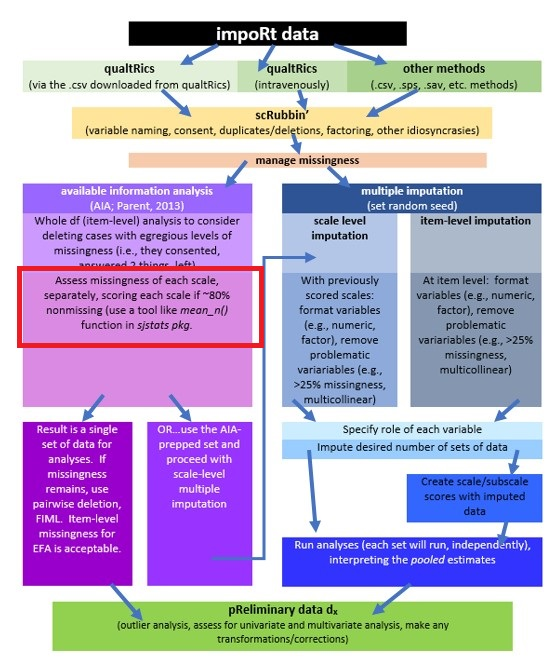
\includegraphics{images/Ch02/wrkflow_scale_lvl.jpg}
\caption{An image of our stage in the workflow for scrubbing and scoring data.}
\end{figure}

First let's get the df down to the variables we want to retain:

\begin{Shaded}
\begin{Highlighting}[]
\NormalTok{scored }\OtherTok{\textless{}{-}}\NormalTok{ dplyr}\SpecialCharTok{::}\FunctionTok{select}\NormalTok{(scrub\_df, iBIPOC\_pr, cmBlack, Belonging, ResponseBL,}
\NormalTok{    StigmaBL, ClimateBL)}
\NormalTok{ScoredCaseMiss }\OtherTok{\textless{}{-}} \FunctionTok{nrow}\NormalTok{(scored)  }\CommentTok{\#I produced this object for the sole purpose of feeding the number of cases into the inline text, below}
\NormalTok{ScoredCaseMiss}
\end{Highlighting}
\end{Shaded}

\begin{verbatim}
## [1] 66
\end{verbatim}

Before we start our formal analysis of missingness at the scale level, let's continue to scrub by eliminating cases that will have too much missingness. In the script below we create a variable that counts the number of missing variables and then creates a proportion by dividing it by the number of total variables.

Using the \emph{describe()} function from the \emph{psych} package, we can investigate this variable.

\begin{Shaded}
\begin{Highlighting}[]
\CommentTok{\# Create a variable (n\_miss) that counts the number missing}
\NormalTok{scored}\SpecialCharTok{$}\NormalTok{n\_miss }\OtherTok{\textless{}{-}}\NormalTok{ scored }\SpecialCharTok{\%\textgreater{}\%}
\NormalTok{    dplyr}\SpecialCharTok{::}\FunctionTok{select}\NormalTok{(iBIPOC\_pr}\SpecialCharTok{:}\NormalTok{ClimateBL) }\SpecialCharTok{\%\textgreater{}\%}
\NormalTok{    is.na }\SpecialCharTok{\%\textgreater{}\%}
\NormalTok{    rowSums}

\CommentTok{\# Create a proportion missing by dividing n\_miss by the total number}
\CommentTok{\# of variables (6) Pipe to sort in order of descending frequency to}
\CommentTok{\# get a sense of the missingness}
\NormalTok{scored }\OtherTok{\textless{}{-}}\NormalTok{ scored }\SpecialCharTok{\%\textgreater{}\%}
\NormalTok{    dplyr}\SpecialCharTok{::}\FunctionTok{mutate}\NormalTok{(}\AttributeTok{prop\_miss =}\NormalTok{ (n\_miss}\SpecialCharTok{/}\DecValTok{6}\NormalTok{) }\SpecialCharTok{*} \DecValTok{100}\NormalTok{) }\SpecialCharTok{\%\textgreater{}\%}
    \FunctionTok{arrange}\NormalTok{(}\FunctionTok{desc}\NormalTok{(n\_miss))}

\NormalTok{psych}\SpecialCharTok{::}\FunctionTok{describe}\NormalTok{(scored}\SpecialCharTok{$}\NormalTok{prop\_miss)}
\end{Highlighting}
\end{Shaded}

\begin{verbatim}
##    vars  n mean    sd median trimmed mad min   max range skew kurtosis   se
## X1    1 66 3.79 12.33      0    0.31   0   0 66.67 66.67 3.44    11.77 1.52
\end{verbatim}

CUMULATIVE CAPTURE FOR WRITING IT UP:

\begin{quote}
\begin{quote}
Across cases that were deemed eligible on the basis of the inclusion/exclusion criteria, missingness ranged from 0 to 100\%. Across the dataset, 3.86\% of cells had missing data and 87.88\% of cases had nonmissing data.
\end{quote}
\end{quote}

\begin{quote}
\begin{quote}
Across the 66 cases for which the scoring protocol was applied, missingness ranged from 0 to 67\%.
\end{quote}
\end{quote}

We need to decide what is our retention threshhold. Twenty percent seems to be a general rule of thumb. Let's delete all cases with missingness at 20\% or greater.

\begin{Shaded}
\begin{Highlighting}[]
\CommentTok{\# update df to have only those with at least 20\% of complete data}
\CommentTok{\# (this is an arbitrary decision)}
\NormalTok{scored }\OtherTok{\textless{}{-}}\NormalTok{ dplyr}\SpecialCharTok{::}\FunctionTok{filter}\NormalTok{(scored, prop\_miss }\SpecialCharTok{\textless{}=} \DecValTok{20}\NormalTok{)}

\CommentTok{\# the variable selection just lops off the proportion missing}
\NormalTok{scored }\OtherTok{\textless{}{-}}\NormalTok{ (}\FunctionTok{select}\NormalTok{(scored, iBIPOC\_pr}\SpecialCharTok{:}\NormalTok{ClimateBL))}

\CommentTok{\# this produces the number of cases retained}
\FunctionTok{nrow}\NormalTok{(scored)}
\end{Highlighting}
\end{Shaded}

\begin{verbatim}
## [1] 61
\end{verbatim}

CUMULATIVE CAPTURE FOR WRITING IT UP:

\begin{quote}
\begin{quote}
Across cases that were deemed eligible on the basis of the inclusion/exclusion criteria, missingness ranged from 0 to 100\%. Across the dataset, 3.86\% of cells had missing data and 87.88\% of cases had nonmissing data.
\end{quote}
\end{quote}

\begin{quote}
\begin{quote}
Across the 66 cases for which the scoring protocol was applied, missingness ranged from 0 to 67\%. After eliminating cases with greater than 20\% missing, the dataset analyzed included 61 cases.
\end{quote}
\end{quote}

With a decision about the number of cases we are going to include, we can continue to analyze missingness.

\hypertarget{revisiting-missing-analysis-at-the-scale-level}{%
\section{Revisiting Missing Analysis at the Scale Level}\label{revisiting-missing-analysis-at-the-scale-level}}

We work with a df that includes only the variables in our model. In our case this is easy. In other cases (i.e., maybe there is an ID number) it might be good to create a subset just for this analysis.

Again, we look at missingness as the proportion of

\begin{itemize}
\tightlist
\item
  individual cells across the scored dataset, and
\item
  rows/cases with nonmissing data
\end{itemize}

\begin{Shaded}
\begin{Highlighting}[]
\CommentTok{\# percent missing across df}
\NormalTok{formattable}\SpecialCharTok{::}\FunctionTok{percent}\NormalTok{(}\FunctionTok{mean}\NormalTok{(}\FunctionTok{is.na}\NormalTok{(scored)))}
\end{Highlighting}
\end{Shaded}

\begin{verbatim}
## [1] 0.55%
\end{verbatim}

\begin{Shaded}
\begin{Highlighting}[]
\CommentTok{\# percent of rows with nonmissing data}
\NormalTok{formattable}\SpecialCharTok{::}\FunctionTok{percent}\NormalTok{(}\FunctionTok{mean}\NormalTok{(}\FunctionTok{complete.cases}\NormalTok{(scored)))}
\end{Highlighting}
\end{Shaded}

\begin{verbatim}
## [1] 96.72%
\end{verbatim}

CUMULATIVE CAPTURE FOR WRITING IT UP:

\begin{quote}
\begin{quote}
Across cases that were deemed eligible on the basis of the inclusion/exclusion criteria, missingness ranged from 0 to 100\%. Across the dataset, 3.86\% of cells had missing data and 87.88\% of cases had nonmissing data.
\end{quote}
\end{quote}

\begin{quote}
\begin{quote}
Across the 66 cases for which the scoring protocol was applied, missingness ranged from 0 to 67\%. After eliminating cases with greater than 20\% missing, the dataset analyzed included 61 cases. In this dataset we had less than 1\% (0.55\%) missing across the df; 97\% of the rows had nonmissing data.
\end{quote}
\end{quote}

Let's look again at missing patterns and mechanisms.

\hypertarget{scale-level-patterns-of-missing-data}{%
\subsection{Scale Level: Patterns of Missing Data}\label{scale-level-patterns-of-missing-data}}

Returning to the \emph{mice} package, we can use the \emph{md.pattern()} function to examine a matrix with the number of columns + 1 in which each row corresponds to a missing data pattern (1 = observed, 0 = missing). The rows and columns are sorted in increasing amounts of missing information. The last column and row contain row and column counts, respectively.

\begin{Shaded}
\begin{Highlighting}[]
\NormalTok{mice\_ScaleLvl }\OtherTok{\textless{}{-}}\NormalTok{ mice}\SpecialCharTok{::}\FunctionTok{md.pattern}\NormalTok{(scored, }\AttributeTok{plot =} \ConstantTok{TRUE}\NormalTok{, }\AttributeTok{rotate.names =} \ConstantTok{TRUE}\NormalTok{)}
\end{Highlighting}
\end{Shaded}

\includegraphics{02-Scoring_files/figure-latex/unnamed-chunk-26-1.pdf}

\begin{Shaded}
\begin{Highlighting}[]
\NormalTok{mice\_ScaleLvl}
\end{Highlighting}
\end{Shaded}

\begin{verbatim}
##    cmBlack Belonging ResponseBL StigmaBL ClimateBL iBIPOC_pr  
## 59       1         1          1        1         1         1 0
## 2        1         1          1        1         1         0 1
##          0         0          0        0         0         2 2
\end{verbatim}

At the scale-level, this is much easier to interpret. There are \emph{2} rows of data because there are only \emph{2} patterns of missingness. The most common pattern is non-missing data (\emph{n} = 59).

If our statistical choice uses listwise deletion (i.e., the case is eliminated if one or more variables in the model has missing data), our sample size will be 59. As we will earn in later chapters, there are alternatives (i.e., specifying a FIML option in analyses that use maximum likelihood estimators) that can use all of the cases -- even those with missing data.

\hypertarget{r-eady-for-analysis}{%
\subsection{R-eady for Analysis}\label{r-eady-for-analysis}}

At this stage the data is ready for analysis (data diagnostics). With the AIA approach \citep{parent_handling_2013} the following preliminary analyses would involve pairwise deletion (i.e., the row/case is dropped for that analysis, but included for all others):

\begin{figure}
\centering
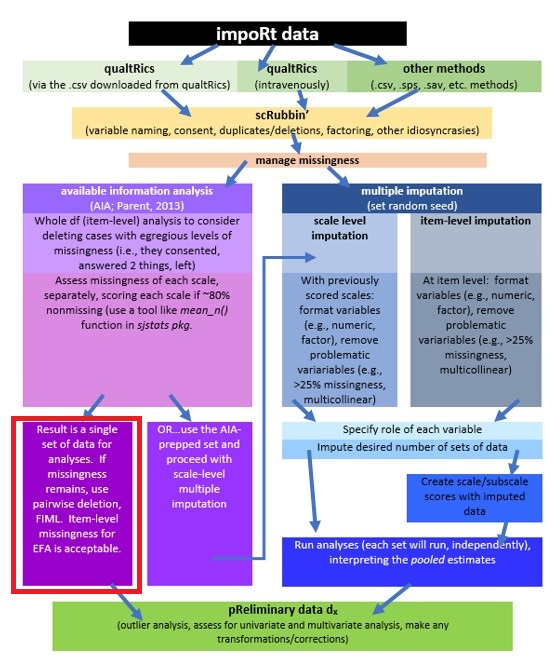
\includegraphics{images/Ch02/wrkflow_AIAready.jpg}
\caption{An image of our stage in the workflow for scrubbing and scoring data.}
\end{figure}

\begin{itemize}
\tightlist
\item
  data diagnostics

  \begin{itemize}
  \tightlist
  \item
    psychometric properties of scales, such as alpha coefficients
  \item
    assessing assumptions such as univariate and multivariate normality, outliers, etc.
  \end{itemize}
\item
  preliminary analyses

  \begin{itemize}
  \tightlist
  \item
    descriptives (means/standard deviations, frequencies)
  \item
    correlation matrices
  \end{itemize}
\end{itemize}

AIA can also be used with primary analyses. Examples of how to manage missingness include:

\begin{itemize}
\tightlist
\item
  ANOVA/regression models

  \begin{itemize}
  \tightlist
  \item
    if completed with ordinary least squares, pairwise deletion would be utilized
  \end{itemize}
\item
  SEM/CFA models with observed, latent, or hybrid models

  \begin{itemize}
  \tightlist
  \item
    if FIML (we'll discuss later) is specified, all cases are used, even when there is missingness
  \end{itemize}
\item
  EFA models

  \begin{itemize}
  \tightlist
  \item
    these can handle item-level missingness
  \end{itemize}
\item
  Hierarchical linear modeling/multilevel modeling/mixed effects modeling

  \begin{itemize}
  \tightlist
  \item
    While all data needs to be present for a given cluster/wave, it is permissible to have varying numbers of clusters/waves per case
  \end{itemize}
\end{itemize}

\hypertarget{the-apa-style-write-up}{%
\section{The APA Style Write-Up}\label{the-apa-style-write-up}}

\hypertarget{results}{%
\section{Results}\label{results}}

\begin{quote}
\begin{quote}
All analyses were completed in R Studio (v. RStudio 2023.06.1+524 ``Mountain Hydrangea'') with R (v. 4.3.1).
\end{quote}
\end{quote}

\begin{quote}
\begin{quote}
\textbf{Missing Data Analysis and Treatment of Missing Data}
\end{quote}
\end{quote}

\begin{quote}
\begin{quote}
Available item analysis (AIA; \citep{parent_handling_2013}) is a strategy for managing missing data that uses available data for analysis and excludes cases with missing data points only for analyses in which the data points would be directly involved. Parent (2013) suggested that AIA is equivalent to more complex methods (e.g., multiple imputation) across a number of variations of sample size, magnitude of associations among items, and degree of missingness. Thus, we utilized Parent's recommendations to guide our approach to managing missing data. Missing data analyses were conducted with tools in base R as well as the R packages, \emph{psych} (v. 2.3.6) and \emph{mice} (v. 3.16.0).
\end{quote}
\end{quote}

\begin{quote}
\begin{quote}
Across cases that were deemed eligible on the basis of the inclusion/exclusion criteria, missingness ranged from 0 to 67\%. Across the dataset, 3.86\% of cells had missing data and 87.88\% of cases had nonmissing data. At this stage in the analysis, we allowed all cases with less than 90\% missing to continue to the scoring stage. Guided by Parent's \citeyearpar{parent_handling_2013} AIA approach, scales with three items were scored if at least two items were non-missing; the scale with four items was scored if it at least three non-missing items; and the scale with six items was scored if it had at least five non-missing items.
\end{quote}
\end{quote}

\begin{quote}
\begin{quote}
Across the 66 cases for which the scoring protocol was applied, missingness ranged from 0 to 67\%. After eliminating cases with greater than 20\% missing, the dataset analyzed included 61 cases. In this dataset we had less than 1\% (0.55\%) missing across the data set; 97\% of the rows had nonmissing data.
\end{quote}
\end{quote}

\hypertarget{practice-problems-1}{%
\section{Practice Problems}\label{practice-problems-1}}

The three problems described below are designed to be continuations from the previous chapter (Scrubbing). You will likely encounter challenges that were not covered in this chapter. Search for and try out solutions, knowing that there are multiple paths through the analysis. The overall notion of the suggestions for practice are to (a) properly format three variables, (b) evaluate item-level missingness, (c) score any scales, (c) evaluate scale-level missingness, (d) provide an APA-style write-up, and (e) explain it to someone.

\hypertarget{problem-1-reworking-the-chapter-problem}{%
\subsection{Problem \#1: Reworking the Chapter Problem}\label{problem-1-reworking-the-chapter-problem}}

If you chose this option in the prior chapter, you imported the data from Qualtrics, applied inclusion/exclusion criteria, renamed variables, downsized the df to the variables of interest, and wrote up the preliminary results.

\hypertarget{problem-2-use-the-rate-a-recent-course-survey-choosing-different-variables-1}{%
\subsection{\texorpdfstring{Problem \#2: Use the \emph{Rate-a-Recent-Course} Survey, Choosing Different Variables}{Problem \#2: Use the Rate-a-Recent-Course Survey, Choosing Different Variables}}\label{problem-2-use-the-rate-a-recent-course-survey-choosing-different-variables-1}}

If you chose this option in the prior chapter, you chose a minimum of three variables from the \emph{Rate-a-Recent-Course} survey to include in a simple statistical model. You imported the dat from Qualtrics, applied inclusion/exclusion criteria, renamed variables, downsized the df to the variables of interest and wrote up the preliminary results.

\hypertarget{problem-3-other-data-1}{%
\subsection{Problem \#3: Other data}\label{problem-3-other-data-1}}

If you chose this option in the prior chapter, you used raw data that was available to you. You imported it into R, applied inclusion/exclusion criteria, renamed variables, downsized the df to the variables of interest, and wrote up the preliminary results.

\hypertarget{grading-rubric-1}{%
\subsection{Grading Rubric}\label{grading-rubric-1}}

\begin{longtable}[]{@{}
  >{\raggedright\arraybackslash}p{(\columnwidth - 4\tabcolsep) * \real{0.7521}}
  >{\centering\arraybackslash}p{(\columnwidth - 4\tabcolsep) * \real{0.1282}}
  >{\centering\arraybackslash}p{(\columnwidth - 4\tabcolsep) * \real{0.1197}}@{}}
\toprule\noalign{}
\begin{minipage}[b]{\linewidth}\raggedright
Assignment Component
\end{minipage} & \begin{minipage}[b]{\linewidth}\centering
Points Possible
\end{minipage} & \begin{minipage}[b]{\linewidth}\centering
Points Earned
\end{minipage} \\
\midrule\noalign{}
\endhead
\bottomrule\noalign{}
\endlastfoot
1. Proper formatting of the items(s) in your first predictor variable & 5 & \_\_\_\_\_ \\
2. Proper formatting of the items(s) in your second predictor variable & 5 & \_\_\_\_\_ \\
3. Proper formatting of the items(s) your third predictor variable & 5 & \_\_\_\_\_ \\
4. Proper formatting of your dependent variable & 5 & \_\_\_\_\_ \\
4. Evaluate and interpret item-level missingness & 5 & \_\_\_\_\_ \\
5. Score any scales/subscales & 5 & \_\_\_\_\_ \\
7. Represent your work in an APA-style write-up (added to the writeup in the previous chapter) & 5 & \_\_\_\_\_ \\
8. Explanation to grader & 5 & \_\_\_\_\_ \\
\textbf{Totals} & 45 & \_\_\_\_\_ \\
\end{longtable}

A \emph{homeworked example} for the Scrubbing, Scoring, and DataDx lessons (combined) follows the \protect\hyperlink{DataDx}{Data Dx} lesson.

\hypertarget{DataDx}{%
\chapter{Data Dx}\label{DataDx}}

\href{https://youtube.com/playlist?list=PLtz5cFLQl4KMSDPjNOLxzIclCsjVypm8n\&si=hIIFTxL2Zby2i8n0}{Screencasted Lecture Link}

The focus of this chapter is \emph{data diagnostics}. We are asking the question, ``Does the data have the appropriate characteristics for the analysis we want to perform?'' Some statistics are more robust than others to violations of the assumptions about the characteristics of the data. None-the-less, we must report these characteristics when we disseminate the results.

\hypertarget{navigating-this-lesson-2}{%
\section{Navigating this Lesson}\label{navigating-this-lesson-2}}

There is about 45 minutes of lecture. If you work through the materials with me it would be plan for an additional hour.

While the majority of R objects and data you will need are created within the R script that sources the chapter, there are a few that cannot be created from within the R framework. Additionally, sometimes links fail. All original materials are provided at the \href{https://github.com/lhbikos/ReC_MultivModel}{Github site} that hosts the book. More detailed guidelines for ways to access all these materials are provided in the OER's \protect\hyperlink{ReCintro}{introduction}

\hypertarget{learning-objectives-2}{%
\subsection{Learning Objectives}\label{learning-objectives-2}}

Learning objectives from this lecture include the following:

\begin{itemize}
\tightlist
\item
  Conduct and interpret critical data diagnostics, including

  \begin{itemize}
  \tightlist
  \item
    alpha coefficients
  \item
    skew
  \item
    kurtosis
  \end{itemize}
\item
  Assess univariate and multivariate normality
\item
  Identify options for managing outliers and skewed data
\item
  Articulate a workflow for data preparation, including scrubbing, scoring, and data diagnostics
\end{itemize}

\hypertarget{planning-for-practice-2}{%
\subsection{Planning for Practice}\label{planning-for-practice-2}}

The suggestions from practice are a continuation from the two prior chapters. If you have completed one or more of those assignments, you should have started with a raw dataset and then scrubbed and scored it. This chapter will involve running basic data diagnostics. Options of graded complexity could incude:

\begin{itemize}
\tightlist
\item
  Repeating the steps in the chapter with the most recent data from the Rate-A-Recent-Course survey; differences will be in the number of people who have completed the survey since the chapter was written.
\item
  Use the dataset that is the source of the chapter, but score a different set of items that you choose.
\item
  Begin with raw data to which you have access.
\end{itemize}

\hypertarget{readings-resources-2}{%
\subsection{Readings \& Resources}\label{readings-resources-2}}

In preparing this chapter, I drew heavily from the following resource(s). Other resources are cited (when possible, linked) in the text with complete citations in the reference list.

\begin{itemize}
\tightlist
\item
  Parent, M. C. (2013). Handling item-level missing data: Simpler is just as good. The Counseling Psychologist, 41(4), 568--600. \url{https://doi.org/10.1177/0011000012445176}

  \begin{itemize}
  \tightlist
  \item
    The purpose of Parent's article was to argue that complex and resource-intensive procedurs like multiple imputation are unnecessary. Following a simulation that supports his claims, Parent provides some guidelines to follow for the AIA approach.
  \end{itemize}
\item
  Kline, R. B. (2016). Data preparation and psychometrics review. In Principles and Practice of Structural Equation Modeling, Fourth Edition. Guilford Publications. \url{http://ebookcentral.proquest.com/lib/spu/detail.action?docID=4000663}

  \begin{itemize}
  \tightlist
  \item
    Kline's chapter is my ``go-to'' for making decisions about preparing data for analysis.
  \end{itemize}
\end{itemize}

\hypertarget{packages-2}{%
\subsection{Packages}\label{packages-2}}

The packages used in this lesson are embedded in this code. When the hashtags are removed, the script below will (a) check to see if the following packages are installed on your computer and, if not (b) install them.

\begin{Shaded}
\begin{Highlighting}[]
\CommentTok{\# if(!require(tidyverse))\{install.packages(\textquotesingle{}tidyverse\textquotesingle{})\} \#this}
\CommentTok{\# includes dplyr if(!require(psych))\{install.packages(\textquotesingle{}psych\textquotesingle{})\}}
\CommentTok{\# if(!require(apaTables))\{install.packages(\textquotesingle{}apaTables\textquotesingle{})\}}
\end{Highlighting}
\end{Shaded}

\hypertarget{workflow-for-preliminary-data-diagnostics}{%
\section{Workflow for Preliminary Data Diagnostics}\label{workflow-for-preliminary-data-diagnostics}}

The same workflow guides us through the Scrubbing, Scoring, and Data Dx chapters. At this stage we have

\begin{itemize}
\tightlist
\item
  imported our raw data from Qualtrics,
\item
  scrubbed the data by applying our inclusion and exclusion criteria, and
\item
  used Parent's available information approach {[}AIA; -\citet{parent_handling_2013}{]} for determining the acceptable amount of missingness for each scale, and
\item
  prepared variables and scored them.
\end{itemize}

We are now ready to engage in data diagnostics for the statistical model we will test.

\begin{figure}
\centering
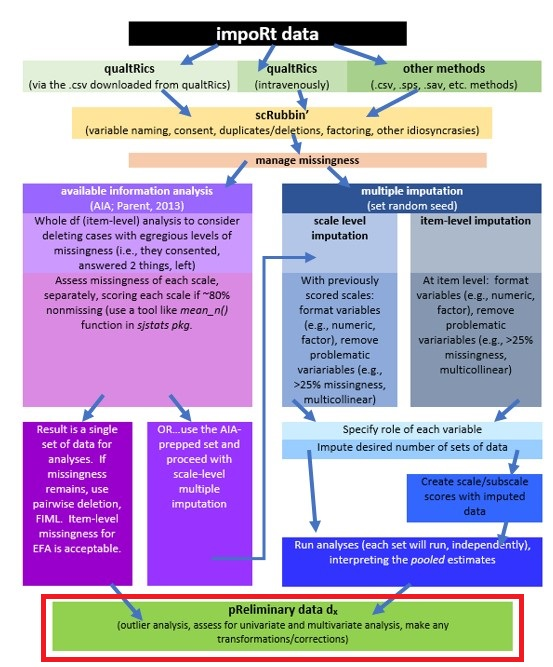
\includegraphics{images/Ch04/wrkflow_dx.jpg}
\caption{An image of our stage in the workflow for scrubbing and scoring data.}
\end{figure}

\hypertarget{research-vignette-2}{%
\section{Research Vignette}\label{research-vignette-2}}

The research vignette comes from the survey titled, \href{https://spupsych.az1.qualtrics.com/jfe/form/SV_b2cClqAlLGQ6nLU}{Rate-a-Recent-Course: A ReCentering Psych Stats Exercise} and is explained in the \protect\hyperlink{scrub}{scrubbing chapter}. In the \protect\hyperlink{score}{scoring chapter} we prepared four variables for analysis. Details for these are in our \href{./Rate-a-Course_Codebook.pdf}{codebook}.

Variable recap:

\begin{itemize}
\tightlist
\item
  Perceived Campus Climate for Black Students includes 6 items, one of which was reverse scored. This scale was adapted from Szymanski et al.'s \citeyearpar{szymanski_perceptions_2020} Campus Climate for LGBTQ students. It has not been evaluated for use with other groups. The Szymanski et al.~analysis suggested that it could be used as a total scale score, or divided into three items each that assess

  \begin{itemize}
  \tightlist
  \item
    College response to LGBTQ students (items 6, 4, 1)
  \item
    LGBTQ stigma (items 3, 2, 5)
  \end{itemize}
\item
  Sense of Belonging includes 3 items. This is a subscale from Bollen and Hoyle's \citeyearpar{bollen_perceived_1990} Perceived Cohesion Scale. There are no items on this scale that require reversing.
\item
  Percent of Black classmates is a single item that asked respondents to estimate the proportion of students in various racial categories
\item
  Percent of BIPOC instructional staff, similarly, asked respondents to identify the racial category of each member of their instructional staff
\end{itemize}

As we noted in the \protect\hyperlink{scrub}{scrubbing chapter}, our design has notable limitations. Briefly, (a) owing to the open source aspect of the data we do not ask about the demographic characteristics of the respondent; (b) the items that ask respondents to \emph{guess} the identities of the instructional staff and to place them in broad categories, (c) we do not provide a ``write-in'' a response. We made these decisions after extensive conversation with stakeholders. The primary reason for these decisions was to prevent potential harm (a) to respondents who could be identified if/when the revealed private information in this open-source survey, and (b) trolls who would write inappropriate or harmful comments.

As I think about ``how these variables go together'' (which is often where I start in planning a study), imagine a parallel mediation. That is the perception of campus climate for Black students would be predicted by the respondent's sense of belonging, mediated in separate paths through the proportion of classmates who are Black and the proportion of BIPOC instructional staff.

\emph{I would like to assess the model by having the instructional staff variable to be the \%Black instructional staff. At the time that this lecture is being prepared, there is not sufficient Black representation in the staff to model this.}

\begin{figure}
\centering
\includegraphics{images/Ch04/BlStuMed.jpg}
\caption{An image of the statistical model for which we are preparing data.}
\end{figure}

I will finish up this chapter by conducting a regression. Because parallel mediation can be complicated (I teach it in a later chapter), I will demonstrate use of our prepared variables with a simple multiple regression.

\begin{figure}
\centering
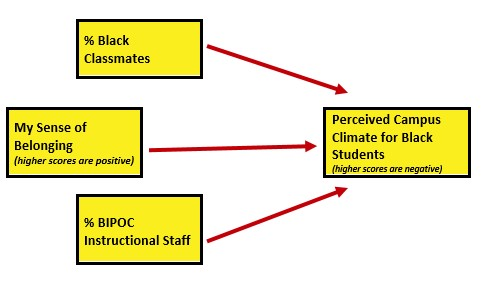
\includegraphics{images/Ch04/BlStuRegression.jpg}
\caption{An image of the statistical model for which we are preparing data.}
\end{figure}

First, though, let's take a more conceptual look at issues regarding missing data. We'll come back to details of the survey as we work with it.

\hypertarget{internal-consistency-of-scalessubscales}{%
\section{Internal Consistency of Scales/Subscales}\label{internal-consistency-of-scalessubscales}}

Alpha coefficients are \emph{reliability coefficients} that assess the \emph{internal consistency} of an instrument. It asks, ``For each person, are responses \emph{consistently} high, or medium, or low?'' To the degree that they are (meaning there are high inter-item correlations), the internal consistency coefficient will be high. We want values \textgreater.80. There are numerous problems with alpha coefficients. The biggest one is that they are influenced by sample size -- longer scales have higher alpha coefficients \citep{cortina_what_1993}. Fourteen seems to be a magic number where we begin to not trust the high alpha coefficient. I address this more thoroughly -- offering an alternative -- in psychometrics. While there is much criticism about the usefulness of the alpha coefficient \citep{sijtsma_use_2009}, researchers continue to use the alpha coefficient as an indicator of the internal consistency of scales that consist of multiple items and contain several variables.

We need item level data to compute an alpha coefficient. The easiest way to get an alpha coefficient is to feed the \emph{alpha()} function (\emph{psych} package) a concatonated list of items (with any items already reverse-scored). There should be no extra items. In the \protect\hyperlink{score}{scoring chapter} we already reverse-coded the single item in the campus climate scale, so we are ready to calculate alphas.

The df from which I am pulling data was created and written as an outfile in the \protect\hyperlink{score}{scoring chapter}. You may also download the file from the \href{https://github.com/lhbikos/ReC_MultivModel}{Github site} that hosts the chapter. Be sure to place the file in the same folder as the .rmd file. This particular df has item-level data. I am working with the .rds file. In case this is problematic for you, I have also provided code to import a .csv version of the file.

\begin{Shaded}
\begin{Highlighting}[]
\NormalTok{item\_scores\_df }\OtherTok{\textless{}{-}} \FunctionTok{readRDS}\NormalTok{(}\StringTok{"BlStItmsScrs230902.rds"}\NormalTok{)}
\CommentTok{\# item\_scores\_df \textless{}{-} read.csv(\textquotesingle{}BlStItmsScrs230902.csv\textquotesingle{}, header = TRUE)}
\end{Highlighting}
\end{Shaded}

Within the \emph{psych::alpha} function we can retrieve alpha coefficients for the specific variables of interest by imbedding a concatonated list. A priori, we are planning to use the campus climate scale as a total score. However, we'll go ahead and also calculate alpha coefficients for the subscales because (a) it's good practice and (b) if the alpha is low, a \emph{reason} might show up in one of the subscales.

\begin{Shaded}
\begin{Highlighting}[]
\CommentTok{\# alpha for the belonging scale}
\NormalTok{psych}\SpecialCharTok{::}\FunctionTok{alpha}\NormalTok{(item\_scores\_df[}\FunctionTok{c}\NormalTok{(}\StringTok{"Belong\_1"}\NormalTok{, }\StringTok{"Belong\_2"}\NormalTok{, }\StringTok{"Belong\_3"}\NormalTok{)])}
\end{Highlighting}
\end{Shaded}

\begin{verbatim}

Reliability analysis   
Call: psych::alpha(x = item_scores_df[c("Belong_1", "Belong_2", "Belong_3")])

  raw_alpha std.alpha G6(smc) average_r S/N    ase mean  sd median_r
      0.95      0.95    0.93      0.87  21 0.0099    4 1.5     0.88

    95% confidence boundaries 
         lower alpha upper
Feldt     0.93  0.95  0.97
Duhachek  0.93  0.95  0.97

 Reliability if an item is dropped:
         raw_alpha std.alpha G6(smc) average_r S/N alpha se var.r med.r
Belong_1      0.94      0.94    0.88      0.88  15    0.016    NA  0.88
Belong_2      0.92      0.92    0.85      0.85  11    0.020    NA  0.85
Belong_3      0.94      0.94    0.89      0.89  16    0.015    NA  0.89

 Item statistics 
          n raw.r std.r r.cor r.drop mean  sd
Belong_1 64  0.95  0.95  0.92   0.90  4.1 1.5
Belong_2 65  0.96  0.96  0.94   0.92  4.1 1.6
Belong_3 64  0.95  0.95  0.91   0.89  3.8 1.5

Non missing response frequency for each item
            1    2    3    4    5    6    7 miss
Belong_1 0.02 0.14 0.23 0.17 0.22 0.17 0.05 0.03
Belong_2 0.03 0.14 0.22 0.22 0.15 0.20 0.05 0.02
Belong_3 0.05 0.19 0.19 0.23 0.20 0.09 0.05 0.03
\end{verbatim}

For each scale I will capture a statement for the APA style write-up. Because these values are typically reported with each measure (and not in the prliminary results), I won't create a cumulative write-up.

\begin{quote}
\begin{quote}
Cronbach's alpha for the belonging scale was 0.95.
\end{quote}
\end{quote}

\begin{Shaded}
\begin{Highlighting}[]
\CommentTok{\# alpha for the campus climate for Black students scale}
\NormalTok{psych}\SpecialCharTok{::}\FunctionTok{alpha}\NormalTok{(item\_scores\_df[}\FunctionTok{c}\NormalTok{(}\StringTok{"rBlst\_1"}\NormalTok{, }\StringTok{"Blst\_2"}\NormalTok{, }\StringTok{"Blst\_3"}\NormalTok{, }\StringTok{"Blst\_4"}\NormalTok{,}
    \StringTok{"Blst\_5"}\NormalTok{, }\StringTok{"Blst\_6"}\NormalTok{)])}
\end{Highlighting}
\end{Shaded}

\begin{verbatim}

Reliability analysis   
Call: psych::alpha(x = item_scores_df[c("rBlst_1", "Blst_2", "Blst_3", 
    "Blst_4", "Blst_5", "Blst_6")])

  raw_alpha std.alpha G6(smc) average_r S/N  ase mean  sd median_r
      0.85      0.87    0.87      0.52 6.5 0.03  2.5 1.1     0.52

    95% confidence boundaries 
         lower alpha upper
Feldt     0.78  0.85  0.90
Duhachek  0.79  0.85  0.91

 Reliability if an item is dropped:
        raw_alpha std.alpha G6(smc) average_r S/N alpha se var.r med.r
rBlst_1      0.85      0.87    0.87      0.57 6.5    0.031 0.029  0.57
Blst_2       0.87      0.88    0.87      0.59 7.1    0.026 0.019  0.56
Blst_3       0.83      0.85    0.85      0.54 5.8    0.034 0.029  0.50
Blst_4       0.80      0.82    0.82      0.48 4.6    0.041 0.027  0.48
Blst_5       0.79      0.81    0.81      0.46 4.3    0.042 0.024  0.47
Blst_6       0.80      0.82    0.81      0.48 4.6    0.040 0.021  0.50

 Item statistics 
         n raw.r std.r r.cor r.drop mean  sd
rBlst_1 60  0.69  0.67  0.56   0.52  3.4 1.6
Blst_2  64  0.68  0.62  0.51   0.46  3.0 1.8
Blst_3  63  0.71  0.74  0.66   0.59  2.0 1.2
Blst_4  62  0.85  0.86  0.84   0.77  2.5 1.3
Blst_5  63  0.89  0.89  0.89   0.82  2.0 1.2
Blst_6  63  0.83  0.86  0.86   0.77  2.1 1.3

Non missing response frequency for each item
           1    2    3    4    5    6    7 miss
rBlst_1 0.10 0.23 0.20 0.25 0.08 0.10 0.03 0.09
Blst_2  0.33 0.16 0.09 0.17 0.16 0.06 0.03 0.03
Blst_3  0.44 0.33 0.06 0.11 0.03 0.02 0.00 0.05
Blst_4  0.27 0.34 0.15 0.18 0.05 0.00 0.02 0.06
Blst_5  0.46 0.30 0.05 0.14 0.05 0.00 0.00 0.05
Blst_6  0.38 0.35 0.11 0.08 0.06 0.02 0.00 0.05
\end{verbatim}

\begin{quote}
\begin{quote}
Cronbach's alpha for the campus climate scale was 0.87.
\end{quote}
\end{quote}

Since this value is \(\geq\) .80, it is within the realm of acceptability. Let's go ahead, though, and examine its subscales.

\begin{Shaded}
\begin{Highlighting}[]
\CommentTok{\# alpha for the stigma scale of the campus climate for Black students}
\CommentTok{\# scale}
\NormalTok{psych}\SpecialCharTok{::}\FunctionTok{alpha}\NormalTok{(item\_scores\_df[}\FunctionTok{c}\NormalTok{(}\StringTok{"Blst\_3"}\NormalTok{, }\StringTok{"Blst\_2"}\NormalTok{, }\StringTok{"Blst\_5"}\NormalTok{)])}
\end{Highlighting}
\end{Shaded}

\begin{verbatim}

Reliability analysis   
Call: psych::alpha(x = item_scores_df[c("Blst_3", "Blst_2", "Blst_5")])

  raw_alpha std.alpha G6(smc) average_r S/N   ase mean  sd median_r
      0.69      0.73    0.69      0.47 2.7 0.065  2.3 1.2     0.54

    95% confidence boundaries 
         lower alpha upper
Feldt     0.54  0.69  0.80
Duhachek  0.57  0.69  0.82

 Reliability if an item is dropped:
       raw_alpha std.alpha G6(smc) average_r  S/N alpha se var.r med.r
Blst_3      0.67      0.70    0.54      0.54 2.35    0.074    NA  0.54
Blst_2      0.75      0.75    0.60      0.60 3.03    0.061    NA  0.60
Blst_5      0.41      0.43    0.28      0.28 0.76    0.135    NA  0.28

 Item statistics 
        n raw.r std.r r.cor r.drop mean  sd
Blst_3 63  0.72  0.78  0.62   0.46    2 1.2
Blst_2 64  0.82  0.75  0.55   0.46    3 1.8
Blst_5 63  0.87  0.89  0.83   0.70    2 1.2

Non missing response frequency for each item
          1    2    3    4    5    6    7 miss
Blst_3 0.44 0.33 0.06 0.11 0.03 0.02 0.00 0.05
Blst_2 0.33 0.16 0.09 0.17 0.16 0.06 0.03 0.03
Blst_5 0.46 0.30 0.05 0.14 0.05 0.00 0.00 0.05
\end{verbatim}

\begin{quote}
\begin{quote}
Cronbach's alpha for the campus climate stigma subscale was 0.73.
\end{quote}
\end{quote}

\begin{Shaded}
\begin{Highlighting}[]
\CommentTok{\# alpha for the campus responsiveness scale of the campus climate for}
\CommentTok{\# Black students scale}
\NormalTok{psych}\SpecialCharTok{::}\FunctionTok{alpha}\NormalTok{(item\_scores\_df[}\FunctionTok{c}\NormalTok{(}\StringTok{"rBlst\_1"}\NormalTok{, }\StringTok{"Blst\_4"}\NormalTok{, }\StringTok{"Blst\_6"}\NormalTok{)])}
\end{Highlighting}
\end{Shaded}

\begin{verbatim}

Reliability analysis   
Call: psych::alpha(x = item_scores_df[c("rBlst_1", "Blst_4", "Blst_6")])

  raw_alpha std.alpha G6(smc) average_r S/N   ase mean  sd median_r
      0.79      0.81    0.76      0.58 4.2 0.045  2.7 1.2     0.52

    95% confidence boundaries 
         lower alpha upper
Feldt     0.69  0.79  0.87
Duhachek  0.71  0.79  0.88

 Reliability if an item is dropped:
        raw_alpha std.alpha G6(smc) average_r S/N alpha se var.r med.r
rBlst_1      0.86      0.86    0.75      0.75 6.0    0.035    NA  0.75
Blst_4       0.64      0.65    0.48      0.48 1.8    0.087    NA  0.48
Blst_6       0.68      0.68    0.52      0.52 2.1    0.078    NA  0.52

 Item statistics 
         n raw.r std.r r.cor r.drop mean  sd
rBlst_1 60  0.81  0.78  0.58   0.53  3.4 1.6
Blst_4  62  0.88  0.89  0.84   0.72  2.5 1.3
Blst_6  63  0.85  0.87  0.81   0.69  2.1 1.3

Non missing response frequency for each item
           1    2    3    4    5    6    7 miss
rBlst_1 0.10 0.23 0.20 0.25 0.08 0.10 0.03 0.09
Blst_4  0.27 0.34 0.15 0.18 0.05 0.00 0.02 0.06
Blst_6  0.38 0.35 0.11 0.08 0.06 0.02 0.00 0.05
\end{verbatim}

\begin{quote}
\begin{quote}
Cronbach's alpha for the campus climate responsiveness subscale was 0.80. Between the two subscales, it looks as if the responsivenes subscale is more internally consistent.
\end{quote}
\end{quote}

\hypertarget{distributional-characteristics-of-the-variables}{%
\section{Distributional Characteristics of the Variables}\label{distributional-characteristics-of-the-variables}}

\hypertarget{evaluating-univariate-normality}{%
\subsection{Evaluating Univariate Normality}\label{evaluating-univariate-normality}}

Statistics like ANOVA and regression each have a set of assumptions about the distributional characteristics of the data. In most of the chapters in this OER we review those assumptions and how to evaluate them. Common across many statistics is the requirement of univariate and multivariate normality. Let's take a look at the variables we will use in our analysis and assess those.

We can continue to work from the df we uploaded at the beginning of the chapter to do this work. Let's take a quick peek. This df has the item-level data (we used it for the alpha coefficients); the scale and subscale scores; and the two items that assess proportion of instructional staff that are BIPOC and proportion of classmates that are BIPOC.

The \emph{str()} function let's us look at the variable format/measurement level of each variable.

\begin{Shaded}
\begin{Highlighting}[]
\FunctionTok{str}\NormalTok{(item\_scores\_df)}
\end{Highlighting}
\end{Shaded}

\begin{verbatim}
Classes 'tbl_df', 'tbl' and 'data.frame':   66 obs. of  17 variables:
 $ ID        : int  1 2 3 4 5 6 7 8 9 10 ...
 $ iBIPOC_pr : num  0.333 0 0.5 0.333 1 ...
 $ cmBlack   : num  0 5 10 6 5 20 0 0 0 4 ...
  ..- attr(*, "label")= Named chr "Regarding race, what proportion of students were from each broad classification.  Your responses should add to 100%. - Black"
  .. ..- attr(*, "names")= chr "Race_1"
 $ Belong_1  : num  6 4 NA 5 4 5 6 7 6 3 ...
  ..- attr(*, "label")= Named chr "Please indicate the degree to which you agree with the following questions about the course. Please skip the it"| __truncated__
  .. ..- attr(*, "names")= chr "Belong_1"
 $ Belong_2  : num  6 4 3 3 4 6 6 7 6 3 ...
  ..- attr(*, "label")= Named chr "Please indicate the degree to which you agree with the following questions about the course. Please skip the it"| __truncated__
  .. ..- attr(*, "names")= chr "Belong_2"
 $ Belong_3  : num  7 6 NA 2 4 5 5 7 6 3 ...
  ..- attr(*, "label")= Named chr "Please indicate the degree to which you agree with the following questions about the course. Please skip the it"| __truncated__
  .. ..- attr(*, "names")= chr "Belong_3"
 $ Blst_1    : num  5 6 NA 2 6 5 5 5 5 3 ...
  ..- attr(*, "label")= Named chr "Each item below asks you to rate elements of campus climate for your \"academic department/program.\"  If you d"| __truncated__
  .. ..- attr(*, "names")= chr "Blst_1"
 $ Blst_2    : num  3 6 5 2 1 1 4 4 3 5 ...
  ..- attr(*, "label")= Named chr "Each item below asks you to rate elements of campus climate for your \"academic department/program.\"  If you d"| __truncated__
  .. ..- attr(*, "names")= chr "Blst_2"
 $ Blst_3    : num  5 2 2 2 1 1 4 3 1 2 ...
  ..- attr(*, "label")= Named chr "Each item below asks you to rate elements of campus climate for your \"academic department/program.\"  If you d"| __truncated__
  .. ..- attr(*, "names")= chr "Blst_3"
 $ Blst_4    : num  2 2 2 2 1 2 4 3 2 3 ...
  ..- attr(*, "label")= Named chr "Each item below asks you to rate elements of campus climate for your \"academic department/program.\"  If you d"| __truncated__
  .. ..- attr(*, "names")= chr "Blst_4"
 $ Blst_5    : num  2 4 NA 2 1 1 4 4 1 3 ...
  ..- attr(*, "label")= Named chr "Each item below asks you to rate elements of campus climate for your \"academic department/program.\"  If you d"| __truncated__
  .. ..- attr(*, "names")= chr "Blst_5"
 $ Blst_6    : num  2 1 2 2 1 2 4 3 2 3 ...
  ..- attr(*, "label")= Named chr "Each item below asks you to rate elements of campus climate for your \"academic department/program.\"  If you d"| __truncated__
  .. ..- attr(*, "names")= chr "Blst_6"
 $ rBlst_1   : num  3 2 NA 6 2 3 3 3 3 5 ...
  ..- attr(*, "label")= Named chr "Each item below asks you to rate elements of campus climate for your \"academic department/program.\"  If you d"| __truncated__
  .. ..- attr(*, "names")= chr "Blst_1"
 $ Belonging : num  6.33 4.67 NA 3.33 4 5.33 5.67 7 6 3 ...
 $ ResponseBL: num  2.33 1.67 2 3.33 1.33 2.33 3.67 3 2.33 3.67 ...
 $ StigmaBL  : num  3.33 4 3.5 2 1 1 4 3.67 1.67 3.33 ...
 $ ClimateBL : num  2.83 2.83 NA 2.67 1.17 1.67 3.83 3.33 2 3.5 ...
 - attr(*, "column_map")=Classes 'tbl_df', 'tbl' and 'data.frame':  182 obs. of  7 variables:
  ..$ qname      : chr [1:182] "StartDate" "EndDate" "Status" "Progress" ...
  ..$ description: chr [1:182] "Start Date" "End Date" "Response Type" "Progress" ...
  ..$ main       : chr [1:182] "Start Date" "End Date" "Response Type" "Progress" ...
  ..$ sub        : chr [1:182] "" "" "" "" ...
  ..$ ImportId   : chr [1:182] "startDate" "endDate" "status" "progress" ...
  ..$ timeZone   : chr [1:182] "America/Los_Angeles" "America/Los_Angeles" NA NA ...
  ..$ choiceId   : chr [1:182] NA NA NA NA ...
\end{verbatim}

The difference between ``int'' (integer) and ``num'' (numerical) is that integers are limited to whole numbers. For the statistics used in this lesson, both are acceptable formats for the variables.

\begin{Shaded}
\begin{Highlighting}[]
\CommentTok{\# the script may look a little complicated; I could have simply}
\CommentTok{\# written: describe(item\_scores\_df) because I only wanted only a few}
\CommentTok{\# variables, I provided them in a concatenated: list [c(\textquotesingle{}iBIPOC\_pr\textquotesingle{},}
\CommentTok{\# \textquotesingle{}cmBlack\textquotesingle{}, \textquotesingle{}Belonging\textquotesingle{}, \textquotesingle{}ClimateBL\textquotesingle{})] I used type =1 so that we can}
\CommentTok{\# interpret skew and kurtosis along Kline\textquotesingle{}s recommendations I created}
\CommentTok{\# an object from the descriptive results, this can be used to export}
\CommentTok{\# the results for easier table making or manipulation outside of R}

\NormalTok{descriptives }\OtherTok{\textless{}{-}}\NormalTok{ psych}\SpecialCharTok{::}\FunctionTok{describe}\NormalTok{(item\_scores\_df[}\FunctionTok{c}\NormalTok{(}\StringTok{"iBIPOC\_pr"}\NormalTok{, }\StringTok{"cmBlack"}\NormalTok{,}
    \StringTok{"Belonging"}\NormalTok{, }\StringTok{"ClimateBL"}\NormalTok{)], }\AttributeTok{type =} \DecValTok{1}\NormalTok{)}
\CommentTok{\# When we capture results in an object, we need to write it below so}
\CommentTok{\# the results will display}
\NormalTok{descriptives}
\end{Highlighting}
\end{Shaded}

\begin{verbatim}
          vars  n mean   sd median trimmed  mad min   max range skew kurtosis
iBIPOC_pr    1 64 0.35 0.39   0.25    0.32 0.37   0  1.00  1.00 0.64    -1.05
cmBlack      2 66 8.20 8.02   5.50    7.24 8.15   0 30.00 30.00 0.95     0.05
Belonging    3 64 4.03 1.47   4.00    4.03 1.48   1  7.00  6.00 0.03    -0.76
ClimateBL    4 61 2.48 1.09   2.33    2.41 0.99   1  5.67  4.67 0.56     0.04
            se
iBIPOC_pr 0.05
cmBlack   0.99
Belonging 0.18
ClimateBL 0.14
\end{verbatim}

\begin{Shaded}
\begin{Highlighting}[]
\CommentTok{\# this can be useful if you wish to manually format the data for an}
\CommentTok{\# APA style table}
\FunctionTok{write.csv}\NormalTok{(descriptives, }\AttributeTok{file =} \StringTok{"DataDx\_descripts.csv"}\NormalTok{)}
\end{Highlighting}
\end{Shaded}

Skew and kurtosis are one way to evaluate whether or not data are normally distributed. When we use the ``type=1'' argument, the skew and kurtosis indices in the \emph{psych} package can be interpreted according to Kline's \citeyearpar{kline_data_2016} guidelines. Regarding skew, values greater than the absolute value of 3.0 are generally considered ``severely skewed.'' Regarding kurtosis, ``severely kurtotic'' is argued to be anywhere greater 8 to 20. Kline recommended using a conservative threshold of the absolute value of 10. The skew and kurtosis values for our variables fall well below these thesholds.

We can also apply the Shapiro-Wilk test of normality to each of our variables. When the \(p\) value is \textless{} .05, the variable's distribution is deviates from a normal distribution to a degree that is statistically significant. Below, the plotting of the histogram with a normal curve superimposed shows how the distribution approximates one that is normal.

\begin{Shaded}
\begin{Highlighting}[]
\CommentTok{\# The shapiro{-}test is in base R; it\textquotesingle{}s specification is simple:}
\CommentTok{\# shapiro.test(df$variable) I added the object (and had to list it}
\CommentTok{\# below) so I can use the inline text function}
\FunctionTok{shapiro.test}\NormalTok{(item\_scores\_df}\SpecialCharTok{$}\NormalTok{cmBlack)}
\end{Highlighting}
\end{Shaded}

\begin{verbatim}

    Shapiro-Wilk normality test

data:  item_scores_df$cmBlack
W = 0.87796, p-value = 0.000009899
\end{verbatim}

\begin{Shaded}
\begin{Highlighting}[]
\FunctionTok{shapiro.test}\NormalTok{(item\_scores\_df}\SpecialCharTok{$}\NormalTok{iBIPOC\_pr)}
\end{Highlighting}
\end{Shaded}

\begin{verbatim}

    Shapiro-Wilk normality test

data:  item_scores_df$iBIPOC_pr
W = 0.78725, p-value = 0.00000003181
\end{verbatim}

\begin{Shaded}
\begin{Highlighting}[]
\FunctionTok{shapiro.test}\NormalTok{(item\_scores\_df}\SpecialCharTok{$}\NormalTok{Belonging)}
\end{Highlighting}
\end{Shaded}

\begin{verbatim}

    Shapiro-Wilk normality test

data:  item_scores_df$Belonging
W = 0.97262, p-value = 0.1654
\end{verbatim}

\begin{Shaded}
\begin{Highlighting}[]
\FunctionTok{shapiro.test}\NormalTok{(item\_scores\_df}\SpecialCharTok{$}\NormalTok{ClimateBL)}
\end{Highlighting}
\end{Shaded}

\begin{verbatim}

    Shapiro-Wilk normality test

data:  item_scores_df$ClimateBL
W = 0.95102, p-value = 0.01613
\end{verbatim}

\hypertarget{pairs-panels}{%
\subsection{Pairs Panels}\label{pairs-panels}}

As we work our way from univariate to multivariate inspection of our data, let's take a look at the bivariate relations.

The \emph{pairs.panels()} function from the \emph{psych} package is useful for showing the relationship between variables (probably no more than 10) in a model.

\begin{itemize}
\tightlist
\item
  The lower half is a scatterplot between the two variables with a regression line (red) and mean (dot).\\
\item
  The diagonal is a histogram of each variable.\\
\item
  The upper half of is the correlation coefficient between the two variables.
\end{itemize}

\begin{Shaded}
\begin{Highlighting}[]
\NormalTok{psych}\SpecialCharTok{::}\FunctionTok{pairs.panels}\NormalTok{(item\_scores\_df[}\FunctionTok{c}\NormalTok{(}\StringTok{"iBIPOC\_pr"}\NormalTok{, }\StringTok{"cmBlack"}\NormalTok{, }\StringTok{"Belonging"}\NormalTok{,}
    \StringTok{"ClimateBL"}\NormalTok{)], }\AttributeTok{stars =} \ConstantTok{TRUE}\NormalTok{, }\AttributeTok{lm =} \ConstantTok{TRUE}\NormalTok{)}
\end{Highlighting}
\end{Shaded}

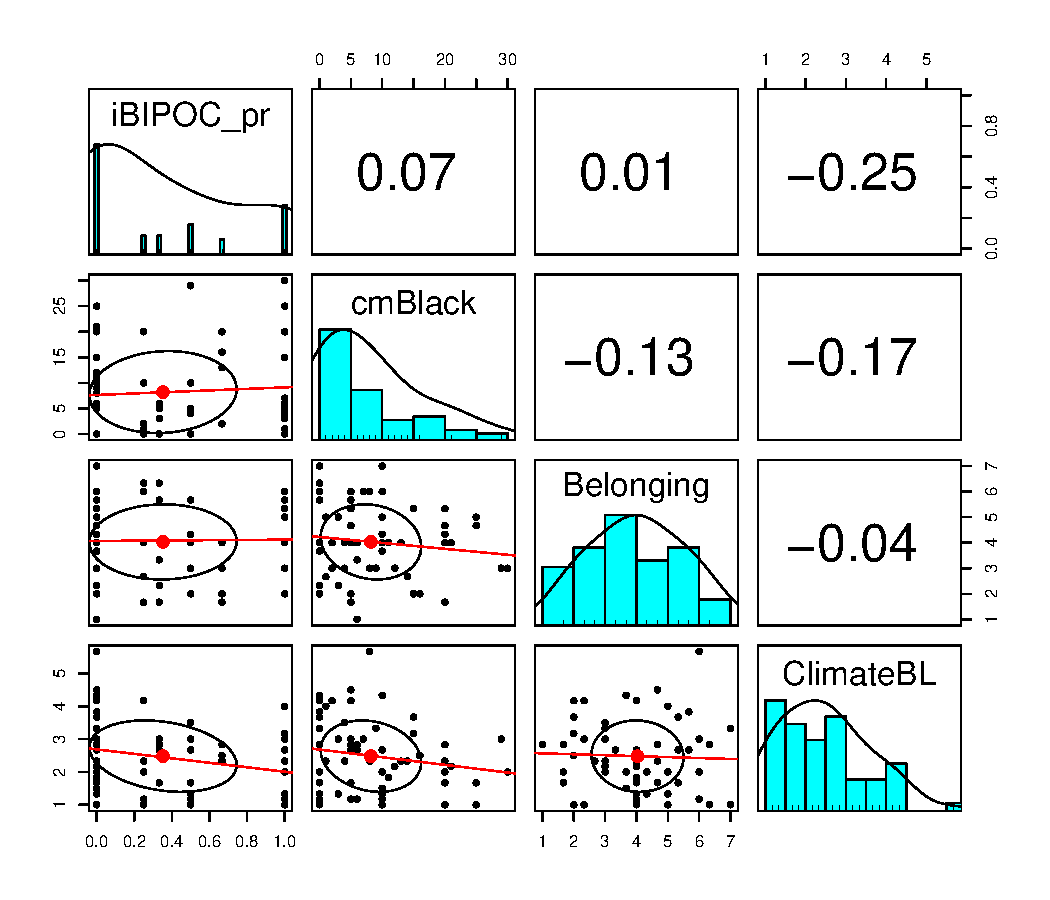
\includegraphics{03-DataDx_files/figure-latex/unnamed-chunk-11-1.pdf}

The histograms displayed in the diagonal graph for us what we learned from the Shapiro Wilk's test of normality. We can clearly see the non-normal distribution in the iBIPOC\_pr and cmBlack variables.

CUMULATIVE CAPTURE FOR THE APA STYLE WRITE-UP:

\begin{quote}
\begin{quote}
Regarding the distributional characteristics of the data, skew and kurtosis values of the variables fell below the values of 3 (skew) and 10 (kurtosis) that Kline suggests are concerning \citeyearpar{kline_principles_2016}. Results of the Shapiro-Wilk test of normality indicate that our variables assessing the proportion of classmates who are Black (\(W = 0.878, p < 0.001\)) and the proportion of BIPOC instructional staff(\(W = 0.787, p < 0.001\)) are statistically significantly different than a normal distribution. Similarly the scale assessing the respondent's perception of campus climate for Black students (\(W = 0.951, p = 0.016\)) differed significantly from a normal distribution. In all three cases the skew values and histograms suggested a somewhat positive skew. That is, there were predominantly low proportions of instructional staff who are BIPOC and classmates who are Black, and the perceptions of campus climate for Black students was evaluated somewhat favorably. The scales assessing the respondent's belonging (\(0.973, p = 0.165\)) did not differ significantly from a normal distribution.
\end{quote}
\end{quote}

What would we do in the case of a univariate outlier? I find Kline's \citeyearpar{kline_principles_2016} chapter on data preparation and management to be extremely useful. He provides ideas for more complex analysis of both univariate and multivariate normality and provides suggestions that range from recoding an extreme value to the next most extreme that is within three standard deviations of the mean to more complicated transformations. First, though we need to further examine the relationships between variables. We do that, next.

\hypertarget{evaluating-multivariate-normality}{%
\section{Evaluating Multivariate Normality}\label{evaluating-multivariate-normality}}

\textbf{Multivariate outliers} have extreme scores on two or more variables, or a pattern of scores that is atypical. For example, a case may have scores between two and three standard deviations above the mean on all variables, even though no case would be extreme. A common method of multivariate outlier detection is the \textbf{Mahalanobis distance} (\(D_{M}^{2}\)). This indicates the distance in variance units between the profile of scores for that case and the vector of sample means, or \textbf{centroid}, correcting for intercorrelations.

The \emph{outlier()} function from the \emph{psych} package tells us how far each datapoint is from the multivariate centroid of the data. That is, find the squared Mahalanobis distance for each data point and compare it to the expected values of \(\chi^2\). The \emph{outlier()} protocol also produces a Q-Q (quantile-quantile) plot with the \emph{n} most extreme data points labeled.

The code below appends the Mahalanobis values to the dataframe. It is easy, then, to identify, sort, and examine the most extreme values (relative to the rest of the data in their case/row) to make decisions about their retention or adjustment.

Numeric variables are required in the of the calculation of the Mahalanobis.

\begin{Shaded}
\begin{Highlighting}[]
\NormalTok{item\_scores\_df}\SpecialCharTok{$}\NormalTok{Mahal }\OtherTok{\textless{}{-}}\NormalTok{ psych}\SpecialCharTok{::}\FunctionTok{outlier}\NormalTok{(item\_scores\_df[}\FunctionTok{c}\NormalTok{(}\StringTok{"iBIPOC\_pr"}\NormalTok{, }\StringTok{"cmBlack"}\NormalTok{,}
    \StringTok{"Belonging"}\NormalTok{, }\StringTok{"ClimateBL"}\NormalTok{)])}
\end{Highlighting}
\end{Shaded}

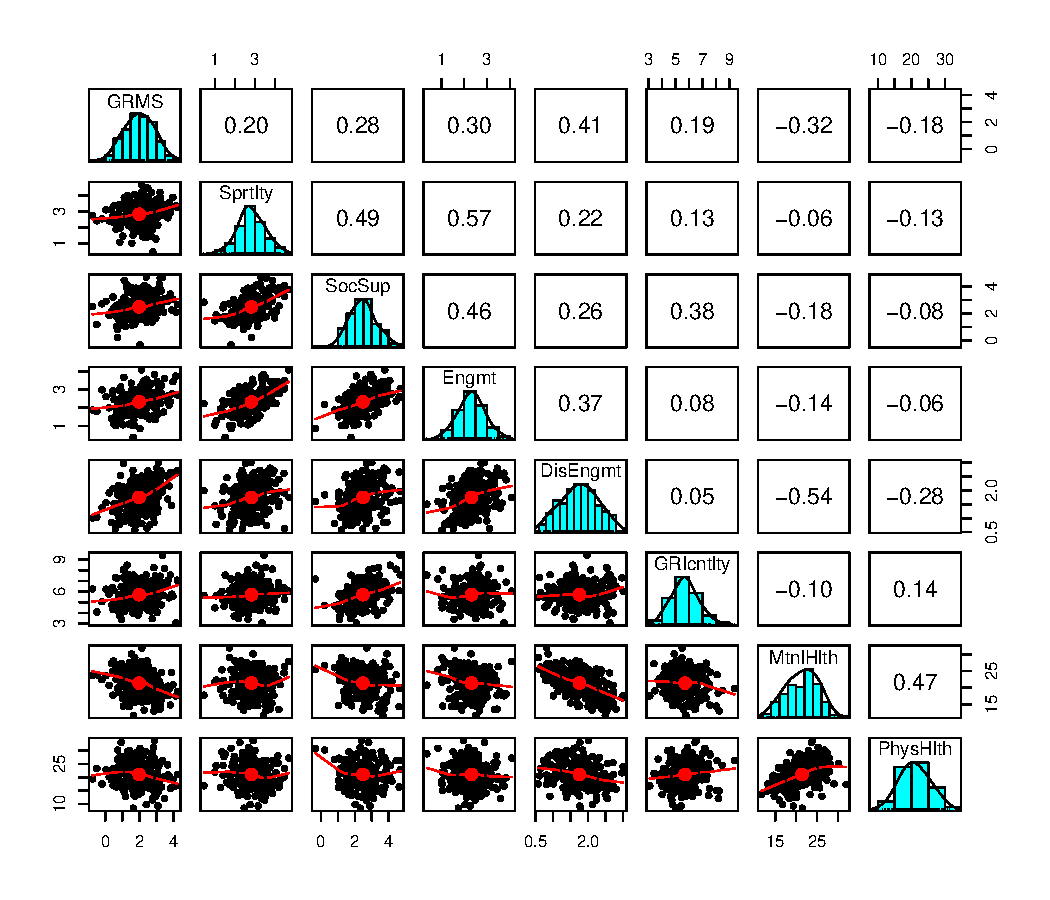
\includegraphics{03-DataDx_files/figure-latex/unnamed-chunk-12-1.pdf}

Q-Q plots take your sample data, sort it in ascending order, and then plot them versus quantiles (the number varies; you can see it on the X axis) calculated from a theoretical distribution. The number of quantiles is selected to match the size of your sample data. While Normal Q-Q Plots are the ones most often used in practice due to so many statistical methods assuming normality, Q-Q Plots can actually be created for any distribution. To the degree that the plotted line stays on the straight line (representing the theoretical normal distribution), the data is multivariate normally distributed.

It is possible, then to analyze the Mahalanobis distance values.

\begin{Shaded}
\begin{Highlighting}[]
\NormalTok{psych}\SpecialCharTok{::}\FunctionTok{describe}\NormalTok{(item\_scores\_df}\SpecialCharTok{$}\NormalTok{Mahal)}
\end{Highlighting}
\end{Shaded}

\begin{verbatim}
   vars  n mean   sd median trimmed  mad min   max range skew kurtosis   se
X1    1 66 3.81 2.24   3.68    3.62 2.36 0.2 11.25 11.05 0.86     0.82 0.28
\end{verbatim}

Using this information we can determine cases that have a Mahalanobis distance values that exceeds three standard deviations around the median. In fact, we can have these noted in a column in the dataframe.

\begin{Shaded}
\begin{Highlighting}[]
\CommentTok{\# creates a variable indicating TRUE or FALSE if an item is an}
\CommentTok{\# outlier}
\NormalTok{item\_scores\_df}\SpecialCharTok{$}\NormalTok{MOutlier }\OtherTok{\textless{}{-}}\NormalTok{ dplyr}\SpecialCharTok{::}\FunctionTok{if\_else}\NormalTok{(item\_scores\_df}\SpecialCharTok{$}\NormalTok{Mahal }\SpecialCharTok{\textgreater{}}\NormalTok{ (}\FunctionTok{median}\NormalTok{(item\_scores\_df}\SpecialCharTok{$}\NormalTok{Mahal) }\SpecialCharTok{+}
\NormalTok{    (}\DecValTok{3} \SpecialCharTok{*} \FunctionTok{sd}\NormalTok{(item\_scores\_df}\SpecialCharTok{$}\NormalTok{Mahal))), }\ConstantTok{TRUE}\NormalTok{, }\ConstantTok{FALSE}\NormalTok{)}

\CommentTok{\# shows us the first 6 rows of the data so we can see the new}
\CommentTok{\# variables (Mahal, MOutlier)}
\FunctionTok{head}\NormalTok{(item\_scores\_df)}
\end{Highlighting}
\end{Shaded}

\begin{verbatim}
# A tibble: 6 x 19
     ID iBIPOC_pr cmBlack Belong_1 Belong_2 Belong_3 Blst_1 Blst_2 Blst_3 Blst_4
  <int>     <dbl>   <dbl>    <dbl>    <dbl>    <dbl>  <dbl>  <dbl>  <dbl>  <dbl>
1     1     0.333       0        6        6        7      5      3      5      2
2     2     0           5        4        4        6      6      6      2      2
3     3     0.5        10       NA        3       NA     NA      5      2      2
4     4     0.333       6        5        3        2      2      2      2      2
5     5     1           5        4        4        4      6      1      1      1
6     6     0          20        5        6        5      5      1      1      2
# i 9 more variables: Blst_5 <dbl>, Blst_6 <dbl>, rBlst_1 <dbl>,
#   Belonging <dbl>, ResponseBL <dbl>, StigmaBL <dbl>, ClimateBL <dbl>,
#   Mahal <dbl>, MOutlier <lgl>
\end{verbatim}

\begin{Shaded}
\begin{Highlighting}[]
\FunctionTok{library}\NormalTok{(tidyverse)}
\end{Highlighting}
\end{Shaded}

\begin{verbatim}
-- Attaching core tidyverse packages ------------------------ tidyverse 2.0.0 --
v dplyr     1.1.2     v readr     2.1.4
v forcats   1.0.0     v stringr   1.5.0
v ggplot2   3.4.3     v tibble    3.2.1
v lubridate 1.9.2     v tidyr     1.3.0
v purrr     1.0.1     
-- Conflicts ------------------------------------------ tidyverse_conflicts() --
x dplyr::filter() masks stats::filter()
x dplyr::lag()    masks stats::lag()
i Use the conflicted package (<http://conflicted.r-lib.org/>) to force all conflicts to become errors
\end{verbatim}

\begin{Shaded}
\begin{Highlighting}[]
\CommentTok{\# counts frequency TRUE and FALSE indicating outlier or not}
\NormalTok{OutlierCount }\OtherTok{\textless{}{-}}\NormalTok{ item\_scores\_df }\SpecialCharTok{\%\textgreater{}\%}
\NormalTok{    dplyr}\SpecialCharTok{::}\FunctionTok{count}\NormalTok{(MOutlier)}

\CommentTok{\# calculating how many outliers a slightly different way}
\FunctionTok{nrow}\NormalTok{(item\_scores\_df) }\SpecialCharTok{{-}}\NormalTok{ OutlierCount}
\end{Highlighting}
\end{Shaded}

\begin{verbatim}
  MOutlier  n
1       66  1
2       65 65
\end{verbatim}

When we identify outliers we often ask if we should delete them or transform the data. A general rule of thumb is to look for ``jumps'' in the Mahalanobis distance values. If they are progressing steadily and there is no ``jump,'' researchers will often retain the outliers.

CUMULATIVE CAPTURE FOR THE APA STYLE WRITE-UP:

\begin{quote}
\begin{quote}
We evaluated multivariate normality with the Mahalanobis distance test. Specifically, we used the \emph{psych::outlier()} function and included all continuous variables in the calculation. Our visual inspection of the Q-Q plot suggested that the plotted line strayed from the straight line as the quantiles increased. Additionally, we appended the Mahalanobis distance scores as a variable to the data. Analyzing this variable, we found that 1 case exceed three standard deviations beyond the median. Given that the Mahalanobis distance values increased in a consistent manner (i.e., no extreme ``jumps'') we retained all cases.
\end{quote}
\end{quote}

\hypertarget{a-few-words-on-transformations}{%
\section{A Few Words on Transformations}\label{a-few-words-on-transformations}}

To quote from Kline \citeyearpar{kline_principles_2016}, ``Before applying a normalizing transformation, you should think about the variables of interest and whether the expectation of normality is reasonable.'' (p.~77)

At this point in history, the non-normal distribution of the proportions of classmates who are Black and instructional staff who are BIPOC are accurate representations in higher education. Kline \citeyearpar{kline_principles_2016} has noted that transforming an inherently non-normal variable to force a normal distribution may fundamentally alter it such that the variable of interest is not actually studied. Kline's chapter reviews some options for applying corrections to outliers. Additionally, the chapter describes a variety of normalizing transformations.

On a personal note, while I will use standardized scores (a linear transformation) if it improves interpretation and center variables around a meaningful intercept, I tend to resist the transformation of data without a really compelling reason. Why? It's complicated and can make interpretation difficult.

\hypertarget{the-apa-style-write-up-1}{%
\section{The APA Style Write-Up}\label{the-apa-style-write-up-1}}

This results section will draw from the three lessons on scrubbing, scoring, and data diagnostics.:

\hypertarget{data-diagnostics}{%
\subsection{Data Diagnostics}\label{data-diagnostics}}

\begin{quote}
\begin{quote}
Data screening suggested that 107 individuals opened the survey link. Of those, 83 granted consent and proceeded into the survey items. A further inclusion criteria was that the course was taught in the U.S; 69 met this criteria.
\end{quote}
\end{quote}

\begin{quote}
\begin{quote}
Available item analysis (AIA; \citep{parent_handling_2013}) is a strategy for managing missing data that uses available data for analysis and excludes cases with missing data points only for analyses in which the data points would be directly involved. Parent (2013) suggested that AIA is equivalent to more complex methods (e.g., multiple imputation) across a number of variations of sample size, magnitude of associations among items, and degree of missingness. Thus, we utilized Parent's recommendations to guide our approach to managing missing data. Missing data analyses were conducted with tools in base R as well as the R packages, \emph{psych} (v. 2.3.6) and \emph{mice} (v. 3.16.0).
\end{quote}
\end{quote}

\begin{quote}
\begin{quote}
Across cases that were deemed eligible on the basis of the inclusion/exclusion criteria, missingness ranged from 0 to 67\%. Across the dataset, 3.86\% of cells had missing data and 87.88\% of cases had nonmissing data. At this stage in the analysis, we allowed all cases with less than 90\% missing to continue to the scoring stage. Guided by Parent's \citeyearpar{parent_handling_2013} AIA approach, scales with three items were scored if at least two items were non-missing; the scale with four items was scored if it at least three non-missing items; and the scale with six items was scored if it had at least five non-missing items.
\end{quote}
\end{quote}

\begin{quote}
\begin{quote}
Across the 66 cases for which the scoring protocol was applied, missingness ranged from 0 to 67\%. After eliminating cases with greater than 20\% missing, the dataset analyzed included 61 cases. In this dataset we had less than 1\% (0.55\%) missing across the df; 97\% of the rows had nonmissing data.
\end{quote}
\end{quote}

\begin{quote}
\begin{quote}
Regarding the distributional characteristics of the data, skew and kurtosis values of the variables fell below the values of 3 (skew) and 10 (kurtosis) that Kline suggests are concerning \citeyearpar{kline_principles_2016}. Results of the Shapiro-Wilk test of normality indicate that our variables assessing the proportion of classmates who are Black (\(W = 0.878, p < 0.001\)) and the proportion of BIPOC instructional staff(\(W = 0.787, p < 0.001\)) are statistically significantly different than a normal distribution. The scales assessing the respondent's belonging (\(0.973, p = 0.165\)) and the respondent's perception of campus climate for Black students (\(W = 0.951, p = 0.016\)) did not differ differently from a normal distribution.
\end{quote}
\end{quote}

\begin{quote}
\begin{quote}
We evaluated multivariate normality with the Mahalanobis distance test. Specifically, we used the \emph{psych::outlier()} function and included all continuous variables in the calculation. Our visual inspection of the Q-Q plot suggested that the plotted line strayed from the straight line as the quantiles increased. Additionally, we appended the Mahalanobis distance scores as a variable to the data. Analyzing this variable, we found that 1 case exceed three standard deviations beyond the median. Given that the Mahalanobis distance values increased in a consistent manner (i.e., no extreme ``jumps'') we retained all cases.
\end{quote}
\end{quote}

\begin{quote}
\begin{quote}
Given that our sample sizes were reasonable for the planned analyses and the degree of missingness was low, we used pairwise deletion in our multiple regression analysis.
\end{quote}
\end{quote}

\hypertarget{a-quick-regression-of-our-research-vignette}{%
\section{A Quick Regression of our Research Vignette}\label{a-quick-regression-of-our-research-vignette}}

With some confidence that our scrubbed-and-scored variables are appropriate for analysis, let me conduct the super quick regression that is our research vignette.

\begin{figure}
\centering
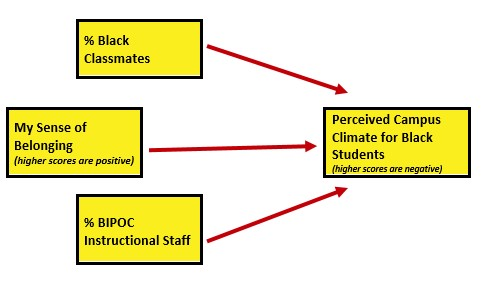
\includegraphics{images/Ch04/BlStuRegression.jpg}
\caption{An image of the statistical model for which we are preparing data.}
\end{figure}

\begin{Shaded}
\begin{Highlighting}[]
\NormalTok{Climate\_fit }\OtherTok{\textless{}{-}} \FunctionTok{lm}\NormalTok{(ClimateBL }\SpecialCharTok{\textasciitilde{}}\NormalTok{ Belonging }\SpecialCharTok{+}\NormalTok{ cmBlack }\SpecialCharTok{+}\NormalTok{ iBIPOC\_pr, }\AttributeTok{data =}\NormalTok{ item\_scores\_df)}
\FunctionTok{summary}\NormalTok{(Climate\_fit)}
\end{Highlighting}
\end{Shaded}

\begin{verbatim}

Call:
lm(formula = ClimateBL ~ Belonging + cmBlack + iBIPOC_pr, data = item_scores_df)

Residuals:
     Min       1Q   Median       3Q      Max 
-1.86732 -0.80535  0.02355  0.70459  3.02003 

Coefficients:
            Estimate Std. Error t value     Pr(>|t|)    
(Intercept)  2.90791    0.46653   6.233 0.0000000674 ***
Belonging   -0.01742    0.09643  -0.181        0.857    
cmBlack     -0.01918    0.01717  -1.117        0.269    
iBIPOC_pr   -0.64125    0.35701  -1.796        0.078 .  
---
Signif. codes:  0 '***' 0.001 '**' 0.01 '*' 0.05 '.' 0.1 ' ' 1

Residual standard error: 1.066 on 55 degrees of freedom
  (7 observations deleted due to missingness)
Multiple R-squared:  0.08212,   Adjusted R-squared:  0.03206 
F-statistic:  1.64 on 3 and 55 DF,  p-value: 0.1906
\end{verbatim}

\hypertarget{results-1}{%
\subsection{Results}\label{results-1}}

\begin{quote}
\begin{quote}
Results of a multiple regression predicting the respondents' perceptions of campus climate for Black students indicated that neither contributions of the respondents' personal belonging (\(B = -0.017, p = -.857\)), the proportion of BIPOC instructional staff (\(B-0.641, p = 0.078), nor the proportion of Black classmates (\)B\$ = -0.019, p = 0.269 ) led to statistically significant changes in perceptions of campus climate for Black students. The model accounted for only 8\% of the variance and was not statistically significant (\(p = 0.191\)). Means, standard deviations, and correlations among variables are presented in Table 1; results of the regression model are presented in Table 2.
\end{quote}
\end{quote}

\begin{Shaded}
\begin{Highlighting}[]
\NormalTok{apaTables}\SpecialCharTok{::}\FunctionTok{apa.cor.table}\NormalTok{(item\_scores\_df[}\FunctionTok{c}\NormalTok{(}\StringTok{"iBIPOC\_pr"}\NormalTok{, }\StringTok{"cmBlack"}\NormalTok{, }\StringTok{"Belonging"}\NormalTok{,}
    \StringTok{"ClimateBL"}\NormalTok{)], }\AttributeTok{table.number =} \DecValTok{1}\NormalTok{, }\AttributeTok{show.sig.stars =} \ConstantTok{TRUE}\NormalTok{, }\AttributeTok{filename =} \StringTok{"Table1\_M\_SDs\_r\_DataDx.doc"}\NormalTok{)}
\end{Highlighting}
\end{Shaded}

\begin{verbatim}


Table 1 

Means, standard deviations, and correlations with confidence intervals
 

  Variable     M    SD   1           2           3          
  1. iBIPOC_pr 0.35 0.39                                    
                                                            
  2. cmBlack   8.20 8.02 .07                                
                         [-.18, .31]                        
                                                            
  3. Belonging 4.03 1.47 .01         -.13                   
                         [-.24, .26] [-.36, .12]            
                                                            
  4. ClimateBL 2.48 1.09 -.25        -.17        -.04       
                         [-.47, .01] [-.41, .08] [-.29, .22]
                                                            

Note. M and SD are used to represent mean and standard deviation, respectively.
Values in square brackets indicate the 95% confidence interval.
The confidence interval is a plausible range of population correlations 
that could have caused the sample correlation (Cumming, 2014).
 * indicates p < .05. ** indicates p < .01.
 
\end{verbatim}

\begin{Shaded}
\begin{Highlighting}[]
\FunctionTok{library}\NormalTok{(apaTables)}
\NormalTok{apaTables}\SpecialCharTok{::}\FunctionTok{apa.reg.table}\NormalTok{(Climate\_fit, }\AttributeTok{table.number =} \DecValTok{2}\NormalTok{, }\AttributeTok{filename =} \StringTok{"Climate\_table.doc"}\NormalTok{)}
\end{Highlighting}
\end{Shaded}

\begin{verbatim}


Table 2 

Regression results using ClimateBL as the criterion
 

   Predictor      b      b_95%_CI  beta   beta_95%_CI sr2  sr2_95%_CI    r
 (Intercept) 2.91**  [1.97, 3.84]                                         
   Belonging  -0.02 [-0.21, 0.18] -0.02 [-0.28, 0.24] .00 [-.01, .01] -.00
     cmBlack  -0.02 [-0.05, 0.02] -0.15 [-0.41, 0.12] .02 [-.05, .09] -.17
   iBIPOC_pr  -0.64 [-1.36, 0.07] -0.23 [-0.49, 0.03] .05 [-.06, .16] -.25
                                                                          
                                                                          
                                                                          
             Fit
                
                
                
                
       R2 = .082
 95% CI[.00,.20]
                

Note. A significant b-weight indicates the beta-weight and semi-partial correlation are also significant.
b represents unstandardized regression weights. beta indicates the standardized regression weights. 
sr2 represents the semi-partial correlation squared. r represents the zero-order correlation.
Square brackets are used to enclose the lower and upper limits of a confidence interval.
* indicates p < .05. ** indicates p < .01.
 
\end{verbatim}

\hypertarget{practice-problems-2}{%
\section{Practice Problems}\label{practice-problems-2}}

The three problems described below are designed to be continuations from the Scrubbing and Scoring lessons. You will likely encounter challenges that were not covered in this chapter. Search for and try out solutions, knowing that there are multiple paths through the analysis. The overall notion of the suggestions for practice are to (a) calculate alpha coefficients for the scales, (b) evaluate univariate and multivariate normality, (c) create an APA-style write-up appropriate for a data diagnostics subsection of the results, and (d) run a ``quickie'' regression, ANOVA, or similar analysis.

\hypertarget{problem-1-reworking-the-chapter-problem-1}{%
\subsection{Problem \#1: Reworking the Chapter Problem}\label{problem-1-reworking-the-chapter-problem-1}}

If you chose this option in the prior chapters, you imported the data from Qualtrics, applied inclusion/exclusion criteria, renamed variables, downsized the df to the variables of interest, properly formatted the variables, interpreted item-level missingness, scored the scales/subscales, interpreted scale-level missingness, and wrote up the results. Please continue with the remaining tasks.

\hypertarget{problem-2-use-the-rate-a-recent-course-survey-choosing-different-variables-2}{%
\subsection{\texorpdfstring{Problem \#2: Use the \emph{Rate-a-Recent-Course} Survey, Choosing Different Variables}{Problem \#2: Use the Rate-a-Recent-Course Survey, Choosing Different Variables}}\label{problem-2-use-the-rate-a-recent-course-survey-choosing-different-variables-2}}

If you chose this option in the prior chapter, you chose a minimum of three variables (different from those in the cahpter) from the \emph{Rate-a-Recent-Course} survey to include in a simple statistical model. You imported the data from Qualtrics, applied inclusion/exclusion criteria, renamed variables, downsized the df to the variables of interest, properly formatted the variables, interpreted item-level missingness, scored the scales/subscales, interpreted scale-level missingness, and wrote up the results. Please continue with the remaining tasks.

\hypertarget{problem-3-other-data-2}{%
\subsection{Problem \#3: Other data}\label{problem-3-other-data-2}}

If you chose this option in the prior chapter, you used raw data that was available to you. You imported it into R, applied inclusion/exclusion criteria, renamed variables, downsized the df to the variables of interest, properly formatted the variables, interpreted item-level missingness, scored the scales/subscales, interpreted scale-level missingness, and wrote up the results. Please continue with the remaining tasks.

\hypertarget{grading-rubric-2}{%
\subsection{Grading Rubric}\label{grading-rubric-2}}

\begin{longtable}[]{@{}
  >{\raggedright\arraybackslash}p{(\columnwidth - 4\tabcolsep) * \real{0.7642}}
  >{\centering\arraybackslash}p{(\columnwidth - 4\tabcolsep) * \real{0.1220}}
  >{\centering\arraybackslash}p{(\columnwidth - 4\tabcolsep) * \real{0.1138}}@{}}
\toprule\noalign{}
\begin{minipage}[b]{\linewidth}\raggedright
Assignment Component
\end{minipage} & \begin{minipage}[b]{\linewidth}\centering
\end{minipage} & \begin{minipage}[b]{\linewidth}\centering
\end{minipage} \\
\midrule\noalign{}
\endhead
\bottomrule\noalign{}
\endlastfoot
1. Calculate alpha coefficients for scales/subscales. & 5 & \_\_\_\_\_ \\
2. Evaluate univariate normality (skew, kurtosis, Shapiro-Wilks). & 5 & \_\_\_\_\_ \\
3. Evaluate multivariate normality (Mahalanobis test) & 5 & \_\_\_\_\_ \\
4. Represent your work in an APA-style write-up (added to the writeup in the previous chapter) & 5 & \_\_\_\_\_ \\
5. Conduct a quick analysis (e.g., regression, ANOVA) including at least three predictor variables & 5 & \_\_\_\_\_ \\
6. Explanation to grader & 5 & \_\_\_\_\_ \\
\textbf{Totals} & 30 & \_\_\_\_\_ \\
\end{longtable}

\hypertarget{homeworked-example}{%
\section{Homeworked Example}\label{homeworked-example}}

\href{https://youtube.com/playlist?list=PLtz5cFLQl4KOZBkREeIJ5Wm_QhX7Pi4un\&si=1aV0H5pJOtbnzWYI}{Screencast Link}

For more information about the data used in this homeworked example, please refer to the description and codebook located at the end of the \href{https://lhbikos.github.io/ReCenterPsychStats/ReCintro.html\#introduction-to-the-data-set-used-for-homeworked-examples}{introductory lesson} in \href{https://lhbikos.github.io/ReCenterPsychStats/}{ReCentering Psych Stats}. An .rds file which holds the data is located in the \href{https://github.com/lhbikos/ReC_MultivModel/tree/main/Worked_Examples}{Worked Examples} folder at the GitHub site the hosts the OER. The file name is \emph{ReC.rds}.

Although the lessons focused on preparing data for analyses were presented in smaller sections, this homeworked example combines the suggestions for practice from the \protect\hyperlink{scrub}{Scrubbing}, \protect\hyperlink{scrub}{Scoring}, and \protect\hyperlink{datadx}{Data Dx} lessons. My hope is that is cumulative presentation is a closer approximation of what researchers need for their research projects.

These lessons were created to prepare a set of data to analyze a specific research model. Consequently, the model should be known and described at the beginning.

\hypertarget{scrubbing-1}{%
\subsection{Scrubbing}\label{scrubbing-1}}

\hypertarget{specify-a-research-model}{%
\subsubsection*{Specify a research model}\label{specify-a-research-model}}


A further requirement was that the model should include three predictor variables (continuously or categorically scaled) and one dependent (continuously scaled) variable.

I am hypothesizing that socially responsive pedagogy (my dependent variable) will increase as a function of:

\begin{itemize}
\tightlist
\item
  the transition from SPSS (0) to R(1),
\item
  the transition from a pre-centered (0) to re-centered (1) curriculum, and
\item
  higher evaluations of traditional pedagogy
\end{itemize}

Because this data is nested within the person (i.e., students can contribute up to three course evaluations over the ANOVA, multivariate, and psychometrics courses) proper analysis would require a statistic (e.g., multilevel modeling) that would address the dependency in the data. Therefore, I will include only those students who are taking the multivariate modeling class.

\emph{If you wanted to use this example and dataset as a basis for a homework assignment, you could create a different subset of data. I worked the example for students taking the multivariate modeling class. You could choose ANOVA or psychometrics. You could also choose a different combinations of variables.}

\begin{figure}
\centering
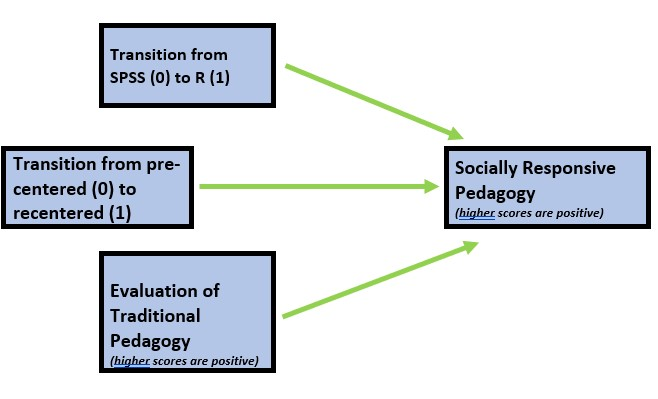
\includegraphics{Worked_Examples/images/homeworked_model.jpg}
\caption{An image of our the prediction model for the homeworked example.}
\end{figure}

\hypertarget{import-data}{%
\subsubsection*{Import data}\label{import-data}}


\begin{Shaded}
\begin{Highlighting}[]
\NormalTok{raw }\OtherTok{\textless{}{-}} \FunctionTok{readRDS}\NormalTok{(}\StringTok{"ReC.rds"}\NormalTok{)}
\FunctionTok{nrow}\NormalTok{(raw)}
\end{Highlighting}
\end{Shaded}

\begin{verbatim}
[1] 310
\end{verbatim}

\hypertarget{include-only-those-who-consented}{%
\subsubsection*{Include only those who consented}\label{include-only-those-who-consented}}


Because this data is publicly posted on the Open Science Framework, it was necessary for me to already exclude those individuals. This data was unique in that students could freely write some version of ``Opt out.'' My original code included a handful of versions, but here was the basic form:

\begin{Shaded}
\begin{Highlighting}[]
\CommentTok{\# testing to see if my code worked raw \textless{}{-} dplyr::filter (raw,}
\CommentTok{\# SPFC.Decolonize.Opt.Out != \textquotesingle{}Okay\textquotesingle{})}
\NormalTok{raw }\OtherTok{\textless{}{-}}\NormalTok{ dplyr}\SpecialCharTok{::}\FunctionTok{filter}\NormalTok{(raw, SPFC.Decolonize.Opt.Out }\SpecialCharTok{!=} \StringTok{"Opt Out"}\NormalTok{)}
\end{Highlighting}
\end{Shaded}

\hypertarget{apply-exclusionary-criteria}{%
\subsubsection*{Apply exclusionary criteria}\label{apply-exclusionary-criteria}}


I want to exclude students' responses for the ANOVA and psychometrics courses.

\begin{Shaded}
\begin{Highlighting}[]
\NormalTok{raw }\OtherTok{\textless{}{-}}\NormalTok{ (dplyr}\SpecialCharTok{::}\FunctionTok{filter}\NormalTok{(raw, Course }\SpecialCharTok{==} \StringTok{"Multivariate"}\NormalTok{))}
\end{Highlighting}
\end{Shaded}

At this point, these my only inclusion/exclusion criteria. I can determine how many students (who consented) completed any portion of the survey.

\begin{Shaded}
\begin{Highlighting}[]
\FunctionTok{nrow}\NormalTok{(raw)}
\end{Highlighting}
\end{Shaded}

\begin{verbatim}
[1] 84
\end{verbatim}

\hypertarget{rename-variables-to-be-sensible-and-systematic}{%
\subsubsection*{Rename variables to be sensible and systematic}\label{rename-variables-to-be-sensible-and-systematic}}


Because this dataset is already on the OSF, the variables are sensibly named. However, I don't like ``SPFC.Decolonize.Opt.Out''. I will change it to simply ``OptOut.''

\begin{Shaded}
\begin{Highlighting}[]
\NormalTok{raw }\OtherTok{\textless{}{-}}\NormalTok{ dplyr}\SpecialCharTok{::}\FunctionTok{rename}\NormalTok{(raw, }\AttributeTok{OptOut =} \StringTok{"SPFC.Decolonize.Opt.Out"}\NormalTok{)}
\end{Highlighting}
\end{Shaded}

It would have made more sense to do this before I used this variable in the calculations.

\hypertarget{downsize-the-dataframe-to-the-variables-of-interest}{%
\subsubsection*{Downsize the dataframe to the variables of interest}\label{downsize-the-dataframe-to-the-variables-of-interest}}


I will need to include:

\begin{itemize}
\tightlist
\item
  deID
\item
  StatsPkg
\item
  Centering
\item
  Items included in the traditional pedagogy scale: ClearResponsibilities, EffectiveAnswers, Feedback, ClearOrganization, ClearPresentation
\item
  Items included in the socially responsive pedagogy scale: InclusvClassrm, EquitableEval, MultPerspectives, DEIintegration
\end{itemize}

\begin{Shaded}
\begin{Highlighting}[]
\NormalTok{scrub\_df }\OtherTok{\textless{}{-}}\NormalTok{ (dplyr}\SpecialCharTok{::}\FunctionTok{select}\NormalTok{(raw, deID, StatsPkg, Centering, ClearResponsibilities,}
\NormalTok{    EffectiveAnswers, Feedback, ClearOrganization, ClearPresentation, InclusvClassrm,}
\NormalTok{    EquitableEval, MultPerspectives, DEIintegration))}
\end{Highlighting}
\end{Shaded}

\hypertarget{provide-an-apa-style-write-up-of-these-preliminary-steps}{%
\subsubsection*{Provide an APA style write-up of these preliminary steps}\label{provide-an-apa-style-write-up-of-these-preliminary-steps}}


\begin{quote}
\begin{quote}
This is a secondary analysis of data involved in a more comprehensive dataset that included students taking multiple statistics courses (\emph{N} = 310). Having retrieved this data from a repository in the Open Science Framework, only those who consented to participation in the study were included. Data used in these analyses were 84 students who completed the multivariate class.
\end{quote}
\end{quote}

\hypertarget{scoring-1}{%
\subsection{Scoring}\label{scoring-1}}

\hypertarget{proper-formatting-of-the-items-in-your-first-predictor-variable}{%
\subsubsection*{Proper formatting of the item(s) in your first predictor variable}\label{proper-formatting-of-the-items-in-your-first-predictor-variable}}


StatsPkg is a dichotomous variable. It should be structured as a factor with two ordered levels: SPSS, R

Because I am using the .rds form of the data from the OSF, this variable retains the former structure I assigned to it. If I needed to write the code, I would do this:

\begin{Shaded}
\begin{Highlighting}[]
\NormalTok{scrub\_df}\SpecialCharTok{$}\NormalTok{StatsPkg }\OtherTok{\textless{}{-}} \FunctionTok{factor}\NormalTok{(scrub\_df}\SpecialCharTok{$}\NormalTok{StatsPkg, }\AttributeTok{levels =} \FunctionTok{c}\NormalTok{(}\StringTok{"SPSS"}\NormalTok{, }\StringTok{"R"}\NormalTok{))}
\FunctionTok{str}\NormalTok{(scrub\_df}\SpecialCharTok{$}\NormalTok{StatsPkg)}
\end{Highlighting}
\end{Shaded}

\begin{verbatim}
 Factor w/ 2 levels "SPSS","R": 2 2 2 2 2 2 2 2 2 2 ...
\end{verbatim}

\hypertarget{proper-formatting-of-items-in-your-second-predictor-variable}{%
\subsubsection*{Proper formatting of item(s) in your second predictor variable}\label{proper-formatting-of-items-in-your-second-predictor-variable}}


Similarly, Centering is a dichotomous variable. It should be structured as a factor with two ordered levels: Pre, Re.

Because I am using the .rds form of the data from the OSF, this variable retains the former structure I assigned to it. If I needed to write the code, I would do this:

\begin{Shaded}
\begin{Highlighting}[]
\NormalTok{scrub\_df}\SpecialCharTok{$}\NormalTok{Centering }\OtherTok{\textless{}{-}} \FunctionTok{factor}\NormalTok{(scrub\_df}\SpecialCharTok{$}\NormalTok{Centering, }\AttributeTok{levels =} \FunctionTok{c}\NormalTok{(}\StringTok{"Pre"}\NormalTok{, }\StringTok{"Re"}\NormalTok{))}
\FunctionTok{str}\NormalTok{(scrub\_df}\SpecialCharTok{$}\NormalTok{Centering)}
\end{Highlighting}
\end{Shaded}

\begin{verbatim}
 Factor w/ 2 levels "Pre","Re": 2 2 2 2 2 2 2 2 2 2 ...
\end{verbatim}

\hypertarget{proper-formatting-of-the-items-in-your-third-predictor-variable}{%
\subsubsection*{Proper formatting of the item(s) in your third predictor variable}\label{proper-formatting-of-the-items-in-your-third-predictor-variable}}


\hypertarget{proper-formatting-of-the-items-in-your-dependent-variable}{%
\subsubsection*{Proper formatting of the item(s) in your dependent variable}\label{proper-formatting-of-the-items-in-your-dependent-variable}}


The third predictor variable is traditional pedagogy. The dependent variable is socially repsonsive pedagogy. The items that will be used in the scale scores for both of these variables are all continuously scaled and should be identified as ``int'' or ``num.'' None of the items need to be reverse-scored.

\begin{Shaded}
\begin{Highlighting}[]
\FunctionTok{str}\NormalTok{(scrub\_df)}
\end{Highlighting}
\end{Shaded}

\begin{verbatim}
Classes 'data.table' and 'data.frame':  84 obs. of  12 variables:
 $ deID                 : int  11 12 13 14 15 16 17 18 35 19 ...
 $ StatsPkg             : Factor w/ 2 levels "SPSS","R": 2 2 2 2 2 2 2 2 2 2 ...
 $ Centering            : Factor w/ 2 levels "Pre","Re": 2 2 2 2 2 2 2 2 2 2 ...
 $ ClearResponsibilities: int  4 5 5 5 4 3 5 5 3 5 ...
 $ EffectiveAnswers     : int  4 5 5 4 4 3 5 5 4 4 ...
 $ Feedback             : int  4 5 4 4 5 4 5 4 4 5 ...
 $ ClearOrganization    : int  3 5 5 4 4 3 5 5 4 5 ...
 $ ClearPresentation    : int  4 5 5 3 4 2 5 4 5 5 ...
 $ InclusvClassrm       : int  5 5 5 5 5 4 5 5 5 5 ...
 $ EquitableEval        : int  4 5 5 5 4 4 5 4 5 5 ...
 $ MultPerspectives     : int  4 5 5 5 5 5 5 4 5 5 ...
 $ DEIintegration       : int  5 5 5 5 5 5 5 5 5 5 ...
 - attr(*, ".internal.selfref")=<externalptr> 
\end{verbatim}

\hypertarget{evaluate-and-interpret-item-level-missingness}{%
\subsubsection*{Evaluate and interpret item-level missingness}\label{evaluate-and-interpret-item-level-missingness}}


The \emph{scrub\_df} is already downsized to include the item-level raw variables and the ID variable. We can continue using it.

I will create a ``proportion missing'' variable.

In this chunk I first calculate the number of missing (nmiss)

\begin{Shaded}
\begin{Highlighting}[]
\FunctionTok{library}\NormalTok{(tidyverse)}\CommentTok{\#needed because the script has pipes}

\CommentTok{\#Calculating number and proportion of item{-}level missingness}
\NormalTok{scrub\_df}\SpecialCharTok{$}\NormalTok{nmiss }\OtherTok{\textless{}{-}}\NormalTok{ scrub\_df}\SpecialCharTok{\%\textgreater{}\%}
\NormalTok{    dplyr}\SpecialCharTok{::}\FunctionTok{select}\NormalTok{(StatsPkg}\SpecialCharTok{:}\NormalTok{DEIintegration) }\SpecialCharTok{\%\textgreater{}\%} \CommentTok{\#the colon allows us to include all variables between the two listed (the variables need to be in order)}
\NormalTok{    is.na }\SpecialCharTok{\%\textgreater{}\%} 
\NormalTok{    rowSums}

\NormalTok{scrub\_df}\OtherTok{\textless{}{-}}\NormalTok{ scrub\_df}\SpecialCharTok{\%\textgreater{}\%}
\NormalTok{  dplyr}\SpecialCharTok{::}\FunctionTok{mutate}\NormalTok{(}\AttributeTok{prop\_miss =}\NormalTok{ (nmiss}\SpecialCharTok{/}\DecValTok{11}\NormalTok{)}\SpecialCharTok{*}\DecValTok{100}\NormalTok{) }\CommentTok{\#11 is the number of variables included in calculating the proportion}
\end{Highlighting}
\end{Shaded}

We can grab the descriptives for the \emph{prop\_miss} variable to begin to understand our data. I will create an object from it so I can use it with inline

\begin{Shaded}
\begin{Highlighting}[]
\NormalTok{psych}\SpecialCharTok{::}\FunctionTok{describe}\NormalTok{(scrub\_df}\SpecialCharTok{$}\NormalTok{prop\_miss)}
\end{Highlighting}
\end{Shaded}

\begin{verbatim}
   vars  n mean   sd median trimmed mad min   max range skew kurtosis   se
X1    1 84 2.38 6.17      0    0.94   0   0 36.36 36.36 3.29    12.33 0.67
\end{verbatim}

Because I want to use the AIA approach to scoring, I'm not willing to filter out any cases yet. If I wanted to eliminate cases with egregious missing (i.e., like 90\%), here is the code I would use:

\begin{Shaded}
\begin{Highlighting}[]
\NormalTok{scrub\_df }\OtherTok{\textless{}{-}}\NormalTok{ dplyr}\SpecialCharTok{::}\FunctionTok{filter}\NormalTok{(scrub\_df, prop\_miss }\SpecialCharTok{\textless{}=} \DecValTok{90}\NormalTok{)  }\CommentTok{\#update df to have only those with at least 90\% of complete data}
\end{Highlighting}
\end{Shaded}

CUMULATIVE CAPTURE FOR WRITING IT UP:

\begin{quote}
\begin{quote}
Across cases that were deemed eligible on the basis of the inclusion/exclusion criteria, missingness ranged from 0 to 36\%.
\end{quote}
\end{quote}

To analyze missingness at the item level, we need a df that has only the variables of interest. That is, variables like \emph{ID} and the \emph{prop\_miss} and \emph{nmiss} variables we created will interfere with an accurate assessment of missingness. I will update our df to eliminate these.

\begin{Shaded}
\begin{Highlighting}[]
\CommentTok{\# further update to exclude the n\_miss and prop\_miss variables}
\NormalTok{ItemMiss\_df }\OtherTok{\textless{}{-}}\NormalTok{ scrub\_df }\SpecialCharTok{\%\textgreater{}\%}
\NormalTok{    dplyr}\SpecialCharTok{::}\FunctionTok{select}\NormalTok{(}\SpecialCharTok{{-}}\FunctionTok{c}\NormalTok{(deID, nmiss, prop\_miss))}
\end{Highlighting}
\end{Shaded}

Missing data analysis commonly looks at proportions by:

\begin{itemize}
\tightlist
\item
  the entire df
\item
  rows/cases/people
\end{itemize}

\begin{Shaded}
\begin{Highlighting}[]
\CommentTok{\# what proportion of cells missing across entire dataset}
\NormalTok{formattable}\SpecialCharTok{::}\FunctionTok{percent}\NormalTok{(}\FunctionTok{mean}\NormalTok{(}\FunctionTok{is.na}\NormalTok{(ItemMiss\_df)))}
\end{Highlighting}
\end{Shaded}

\begin{verbatim}
[1] 2.38%
\end{verbatim}

\begin{Shaded}
\begin{Highlighting}[]
\CommentTok{\# what proportion of cases (rows) are complete (nonmissing)}
\NormalTok{formattable}\SpecialCharTok{::}\FunctionTok{percent}\NormalTok{(}\FunctionTok{mean}\NormalTok{(}\FunctionTok{complete.cases}\NormalTok{(ItemMiss\_df)))}
\end{Highlighting}
\end{Shaded}

\begin{verbatim}
[1] 82.14%
\end{verbatim}

CUMULATIVE CAPTURE FOR WRITING IT UP:

\begin{quote}
\begin{quote}
Across cases that were deemed eligible on the basis of the inclusion/exclusion criteria, missingness ranged from 0 to 36\%. Across the dataset, 2.38\% of cells had missing data and 82.14\% of cases had nonmissing data.
\end{quote}
\end{quote}

We can further explore patterns of missingness with \emph{mice.md.pattern}.

\begin{Shaded}
\begin{Highlighting}[]
\NormalTok{mice}\SpecialCharTok{::}\FunctionTok{md.pattern}\NormalTok{(ItemMiss\_df, }\AttributeTok{plot =} \ConstantTok{TRUE}\NormalTok{, }\AttributeTok{rotate.names =} \ConstantTok{TRUE}\NormalTok{)}
\end{Highlighting}
\end{Shaded}

There are 6 missingness patterns. The most common (\emph{n} = 69) have no missingness. There are 11 students missing the DEIintegration item (on the traditional pedagogy scale). This item may have been a later addition to the Canvas course evaluations.

Comparing this to Enders' \citeyearpar{enders_applied_2010} \href{https://www.google.com/books/edition/Applied_Missing_Data_Analysis/uHt4EAAAQBAJ?hl=en\&gbpv=1\&dq=enders+missing+data\&pg=PP1\&printsec=frontcover}{prototypical patterns of missingness} (page 3), the \emph{mice} output represents the monotonic pattern often caused by test fatigue. That is, once a student stopped responding, they didn't continue with the rest of the evaluation. That said, this was true of only 4 students (1 each pattern). A quick reminder -- diagnosing monotonicity requires that the variables in the \emph{mice.mdpattern} figures were presented to the research participant in that order.

\hypertarget{score-any-scalessubscales}{%
\subsubsection*{Score any scales/subscales}\label{score-any-scalessubscales}}


Traditional pedagogy is a predictor variable that needs to be created by calculating the mean if at least 75\% of the items are non-missing. None of the items need to be reverse-scored. I will return to working with the \emph{scrub\_df} data.

\begin{Shaded}
\begin{Highlighting}[]
\CommentTok{\# this seems to work when I build the book, but not in \textquotesingle{}working the}
\CommentTok{\# problem\textquotesingle{} TradPed\_vars \textless{}{-} c(\textquotesingle{}ClearResponsibilities\textquotesingle{},}
\CommentTok{\# \textquotesingle{}EffectiveAnswers\textquotesingle{},\textquotesingle{}Feedback\textquotesingle{},}
\CommentTok{\# \textquotesingle{}ClearOrganization\textquotesingle{},\textquotesingle{}ClearPresentation\textquotesingle{}) scrub\_df$TradPed \textless{}{-}}
\CommentTok{\# sjstats::mean\_n(scrub\_df[, TradPed\_vars], .75)}

\CommentTok{\# this seems to work when I \textquotesingle{}work the problem\textquotesingle{} (but not when I build}
\CommentTok{\# the book) the difference is the two dots before the last SRPed\_vars}
\NormalTok{TradPed\_vars }\OtherTok{\textless{}{-}} \FunctionTok{c}\NormalTok{(}\StringTok{"ClearResponsibilities"}\NormalTok{, }\StringTok{"EffectiveAnswers"}\NormalTok{, }\StringTok{"Feedback"}\NormalTok{,}
    \StringTok{"ClearOrganization"}\NormalTok{, }\StringTok{"ClearPresentation"}\NormalTok{)}
\NormalTok{scrub\_df}\SpecialCharTok{$}\NormalTok{TradPed }\OtherTok{\textless{}{-}}\NormalTok{ sjstats}\SpecialCharTok{::}\FunctionTok{mean\_n}\NormalTok{(scrub\_df[, TradPed\_vars], }\FloatTok{0.75}\NormalTok{)}
\end{Highlighting}
\end{Shaded}

The dependent variable is socially responsive pedagogy. It needs to be created by calculating the mean if at least 75\% of the items are non-missing. None of the items need to be reverse-scored.

\begin{Shaded}
\begin{Highlighting}[]
\CommentTok{\# this seems to work when I build the book, but not in \textquotesingle{}working the}
\CommentTok{\# problem\textquotesingle{} SRPed\_vars \textless{}{-} c(\textquotesingle{}InclusvClassrm\textquotesingle{},\textquotesingle{}EquitableEval\textquotesingle{},}
\CommentTok{\# \textquotesingle{}MultPerspectives\textquotesingle{}, \textquotesingle{}DEIintegration\textquotesingle{}) scrub\_df$SRPed \textless{}{-}}
\CommentTok{\# sjstats::mean\_n(scrub\_df[, SRPed\_vars], .75)}

\CommentTok{\# this seems to work when I \textquotesingle{}work the problem\textquotesingle{} (but not when I build}
\CommentTok{\# the book) the difference is the two dots before the last SRPed\_vars}
\NormalTok{SRPed\_vars }\OtherTok{\textless{}{-}} \FunctionTok{c}\NormalTok{(}\StringTok{"InclusvClassrm"}\NormalTok{, }\StringTok{"EquitableEval"}\NormalTok{, }\StringTok{"MultPerspectives"}\NormalTok{,}
    \StringTok{"DEIintegration"}\NormalTok{)}
\NormalTok{scrub\_df}\SpecialCharTok{$}\NormalTok{SRPed }\OtherTok{\textless{}{-}}\NormalTok{ sjstats}\SpecialCharTok{::}\FunctionTok{mean\_n}\NormalTok{(scrub\_df[, SRPed\_vars], }\FloatTok{0.75}\NormalTok{)}
\end{Highlighting}
\end{Shaded}

\hypertarget{evaluate-and-interpret-scale-level-missingness}{%
\subsubsection*{Evaluate and interpret scale-level missingness}\label{evaluate-and-interpret-scale-level-missingness}}


To evaluate scale level missingness, let's create a df with the focal variables.

\begin{Shaded}
\begin{Highlighting}[]
\NormalTok{scored }\OtherTok{\textless{}{-}}\NormalTok{ dplyr}\SpecialCharTok{::}\FunctionTok{select}\NormalTok{(scrub\_df, StatsPkg, Centering, TradPed, SRPed)}
\NormalTok{ScoredCaseMiss }\OtherTok{\textless{}{-}} \FunctionTok{nrow}\NormalTok{(scored)  }\CommentTok{\#I produced this object for the sole purpose of feeding the number of cases into the inline text, below}
\NormalTok{ScoredCaseMiss}
\end{Highlighting}
\end{Shaded}

\begin{verbatim}
[1] 84
\end{verbatim}

Before we start our formal analysis of missingness at the scale level, let's continue to scrub by eliminating cases that will have too much missingness. In the script below we create a variable that counts the number of missing variables and then creates a proportion by dividing it by the number of total variables.

Using the \emph{describe()} function from the \emph{psych} package, we can investigate this variable.

\begin{Shaded}
\begin{Highlighting}[]
\FunctionTok{library}\NormalTok{(tidyverse)}
\CommentTok{\# Create a variable (n\_miss) that counts the number missing}
\NormalTok{scored}\SpecialCharTok{$}\NormalTok{n\_miss }\OtherTok{\textless{}{-}}\NormalTok{ scored }\SpecialCharTok{\%\textgreater{}\%}
\NormalTok{    is.na }\SpecialCharTok{\%\textgreater{}\%}
\NormalTok{    rowSums}

\CommentTok{\# Create a proportion missing by dividing n\_miss by the total number}
\CommentTok{\# of variables (6) Pipe to sort in order of descending frequency to}
\CommentTok{\# get a sense of the missingness}
\NormalTok{scored }\OtherTok{\textless{}{-}}\NormalTok{ scored }\SpecialCharTok{\%\textgreater{}\%}
    \FunctionTok{mutate}\NormalTok{(}\AttributeTok{prop\_miss =}\NormalTok{ (n\_miss}\SpecialCharTok{/}\DecValTok{6}\NormalTok{) }\SpecialCharTok{*} \DecValTok{100}\NormalTok{) }\SpecialCharTok{\%\textgreater{}\%}
    \FunctionTok{arrange}\NormalTok{(}\FunctionTok{desc}\NormalTok{(n\_miss))}

\NormalTok{psych}\SpecialCharTok{::}\FunctionTok{describe}\NormalTok{(scored}\SpecialCharTok{$}\NormalTok{prop\_miss)}
\end{Highlighting}
\end{Shaded}

\begin{verbatim}
   vars  n mean   sd median trimmed mad min   max range skew kurtosis   se
X1    1 84 0.79 4.41      0       0   0   0 33.33 33.33 5.89    36.31 0.48
\end{verbatim}

CUMULATIVE CAPTURE FOR WRITING IT UP:

\begin{quote}
\begin{quote}
Across cases that were deemed eligible on the basis of the inclusion/exclusion criteria, missingness ranged from 0 to 36\%. Across the dataset, 2.38\% of cells had missing data and 82.14\% of cases had nonmissing data.
\end{quote}
\end{quote}

\begin{quote}
\begin{quote}
Across the 84 cases for which the scoring protocol was applied, missingness ranged from 0 to 33\%.
\end{quote}
\end{quote}

We need to decide what is our retention threshhold. Twenty percent seems to be a general rule of thumb. Let's delete all cases with missingness at 20\% or greater.

\begin{Shaded}
\begin{Highlighting}[]
\CommentTok{\# update df to have only those with at least 20\% of complete data}
\CommentTok{\# (this is an arbitrary decision)}
\NormalTok{scored }\OtherTok{\textless{}{-}}\NormalTok{ dplyr}\SpecialCharTok{::}\FunctionTok{filter}\NormalTok{(scored, prop\_miss }\SpecialCharTok{\textless{}=} \DecValTok{20}\NormalTok{)}

\CommentTok{\# the variable selection just lops off the proportion missing}
\NormalTok{scored }\OtherTok{\textless{}{-}}\NormalTok{ (}\FunctionTok{select}\NormalTok{(scored, StatsPkg}\SpecialCharTok{:}\NormalTok{SRPed))}

\CommentTok{\# this produces the number of cases retained}
\FunctionTok{nrow}\NormalTok{(scored)}
\end{Highlighting}
\end{Shaded}

\begin{verbatim}
[1] 83
\end{verbatim}

CUMULATIVE CAPTURE FOR WRITING IT UP:

\begin{quote}
\begin{quote}
Across cases that were deemed eligible on the basis of the inclusion/exclusion criteria, missingness ranged from 0 to 100\%. Across the dataset, 3.86\% of cells had missing data and 87.88\% of cases had nonmissing data.
\end{quote}
\end{quote}

\begin{quote}
\begin{quote}
Across the 84 cases for which the scoring protocol was applied, missingness ranged from 0 to 67\%. After eliminating cases with greater than 20\% missing, the dataset analyzed included 83 cases.
\end{quote}
\end{quote}

Now, at the scale level, we look at missingness as the proportion of

\begin{itemize}
\tightlist
\item
  individual cells across the scored dataset, and
\item
  rows/cases with nonmissing data
\end{itemize}

\begin{Shaded}
\begin{Highlighting}[]
\CommentTok{\# percent missing across df}
\NormalTok{formattable}\SpecialCharTok{::}\FunctionTok{percent}\NormalTok{(}\FunctionTok{mean}\NormalTok{(}\FunctionTok{is.na}\NormalTok{(scored)))}
\end{Highlighting}
\end{Shaded}

\begin{verbatim}
[1] 0.60%
\end{verbatim}

\begin{Shaded}
\begin{Highlighting}[]
\CommentTok{\# percent of rows with nonmissing data}
\NormalTok{formattable}\SpecialCharTok{::}\FunctionTok{percent}\NormalTok{(}\FunctionTok{mean}\NormalTok{(}\FunctionTok{complete.cases}\NormalTok{(scored)))}
\end{Highlighting}
\end{Shaded}

\begin{verbatim}
[1] 97.59%
\end{verbatim}

CUMULATIVE CAPTURE FOR WRITING IT UP:

\begin{quote}
\begin{quote}
Across cases that were deemed eligible on the basis of the inclusion/exclusion criteria, missingness ranged from 0 to 100\%. Across the dataset, 3.86\% of cells had missing data and 87.88\% of cases had nonmissing data.
\end{quote}
\end{quote}

\begin{quote}
\begin{quote}
Across the 84 cases for which the scoring protocol was applied, missingness ranged from 0 to 67\%. After eliminating cases with greater than 20\% missing, the dataset analyzed included 83 cases. In this dataset we had less than 1\% (0.60\%) missing across the df; 98\% of the rows had nonmissing data.
\end{quote}
\end{quote}

Let's look again at missing patterns and mechanisms.

Returning to the \emph{mice} package, we can use the \emph{md.pattern()} function to examine a matrix with the number of columns 1 in which each row corresponds to a missing data pattern (0 = observed, 0 = missing). The rows and columns are sorted in increasing amounts of missing information. The last column and row contain row and column counts, respectively.

The corresponding figure shows non-missing data in blue; missing data in red.

\begin{Shaded}
\begin{Highlighting}[]
\NormalTok{mice\_ScaleLvl }\OtherTok{\textless{}{-}}\NormalTok{ mice}\SpecialCharTok{::}\FunctionTok{md.pattern}\NormalTok{(scored, }\AttributeTok{plot =} \ConstantTok{TRUE}\NormalTok{, }\AttributeTok{rotate.names =} \ConstantTok{TRUE}\NormalTok{)}
\end{Highlighting}
\end{Shaded}

\includegraphics{03-DataDx_files/figure-latex/unnamed-chunk-43-1.pdf}

\begin{Shaded}
\begin{Highlighting}[]
\NormalTok{mice\_ScaleLvl}
\end{Highlighting}
\end{Shaded}

\begin{verbatim}
   StatsPkg Centering TradPed SRPed  
81        1         1       1     1 0
2         1         1       1     0 1
          0         0       0     2 2
\end{verbatim}

There are \emph{2} rows of data because there are only \emph{2} patterns of missingness. The most common pattern is non-missing data (\emph{n} = 81). Two cases are missing the SRPed variable. If our statistical choice uses listwise deletion (i.e., the case is eliminated if one or more variables in the model has missing data), our sample size will be 79. As we will earn in later chapters, there are alternatives (i.e., specifying a FIML option in analyses that use maximum likelihood estimators) that can use all of the cases -- even those with missing data.

\hypertarget{represent-your-work-in-an-apa-style-write-up-added-to-the-writeup-in-the-previous-chapter}{%
\subsubsection*{Represent your work in an APA-style write-up (added to the writeup in the previous chapter}\label{represent-your-work-in-an-apa-style-write-up-added-to-the-writeup-in-the-previous-chapter}}


\begin{quote}
\begin{quote}
Available item analysis (AIA; \citep{parent_handling_2013}) is a strategy for managing missing data that uses available data for analysis and excludes cases with missing data points only for analyses in which the data points would be directly involved. Parent (2013) suggested that AIA is equivalent to more complex methods (e.g., multiple imputation) across a number of variations of sample size, magnitude of associations among items, and degree of missingness. Thus, we utilized Parent's recommendations to guide our approach to managing missing data. Missing data analyses were conducted with tools in base R as well as the R packages, \emph{psych} (v. 2.3.6) and \emph{mice} (v. 3.16.0).
\end{quote}
\end{quote}

\begin{quote}
\begin{quote}
Across cases that were deemed eligible on the basis of the inclusion/exclusion criteria, missingness ranged from 0 to 100\%. Across the dataset, 3.86\% of cells had missing data and 87.88\% of cases had nonmissing data.
\end{quote}
\end{quote}

\begin{quote}
\begin{quote}
Across the 84 cases for which the scoring protocol was applied, missingness ranged from 0 to 67\%. After eliminating cases with greater than 20\% missing, the dataset analyzed included 83 cases. In this dataset we had less than 1\% (0.60\%) missing across the df; 98\% of the rows had nonmissing data.
\end{quote}
\end{quote}

\hypertarget{data-dx}{%
\subsection{Data Dx}\label{data-dx}}

\hypertarget{calculate-alpha-coefficients-for-scalessubscales}{%
\subsubsection*{Calculate alpha coefficients for scales/subscales}\label{calculate-alpha-coefficients-for-scalessubscales}}


To calculate the alpha coefficients, we need item-level data. We will return to \emph{scrub\_df} that contains the item-level data.

\begin{Shaded}
\begin{Highlighting}[]
\CommentTok{\# alpha for the traditional pedagogy scale}
\NormalTok{psych}\SpecialCharTok{::}\FunctionTok{alpha}\NormalTok{(scrub\_df[}\FunctionTok{c}\NormalTok{(}\StringTok{"ClearResponsibilities"}\NormalTok{, }\StringTok{"EffectiveAnswers"}\NormalTok{, }\StringTok{"Feedback"}\NormalTok{,}
    \StringTok{"ClearOrganization"}\NormalTok{, }\StringTok{"ClearPresentation"}\NormalTok{)])}
\end{Highlighting}
\end{Shaded}

\begin{verbatim}

Reliability analysis   
Call: psych::alpha(x = scrub_df[c("ClearResponsibilities", "EffectiveAnswers", 
    "Feedback", "ClearOrganization", "ClearPresentation")])

  raw_alpha std.alpha G6(smc) average_r S/N   ase mean   sd median_r
      0.87      0.88    0.87      0.59 7.2 0.022  4.3 0.72     0.58

    95% confidence boundaries 
         lower alpha upper
Feldt     0.83  0.87  0.91
Duhachek  0.83  0.87  0.92

 Reliability if an item is dropped:
                      raw_alpha std.alpha G6(smc) average_r S/N alpha se  var.r
ClearResponsibilities      0.84      0.84    0.82      0.57 5.3    0.029 0.0110
EffectiveAnswers           0.84      0.84    0.81      0.57 5.2    0.029 0.0088
Feedback                   0.87      0.87    0.86      0.64 7.0    0.023 0.0053
ClearOrganization          0.86      0.86    0.83      0.60 6.1    0.025 0.0067
ClearPresentation          0.83      0.84    0.81      0.57 5.3    0.030 0.0074
                      med.r
ClearResponsibilities  0.55
EffectiveAnswers       0.58
Feedback               0.63
ClearOrganization      0.59
ClearPresentation      0.57

 Item statistics 
                       n raw.r std.r r.cor r.drop mean   sd
ClearResponsibilities 83  0.85  0.85  0.80   0.74  4.5 0.87
EffectiveAnswers      84  0.84  0.85  0.82   0.76  4.4 0.79
Feedback              82  0.74  0.75  0.65   0.60  4.3 0.81
ClearOrganization     84  0.82  0.80  0.74   0.68  4.1 1.04
ClearPresentation     84  0.85  0.85  0.81   0.76  4.2 0.87

Non missing response frequency for each item
                         1    2    3    4    5 miss
ClearResponsibilities 0.01 0.05 0.04 0.27 0.64 0.01
EffectiveAnswers      0.02 0.00 0.05 0.40 0.52 0.00
Feedback              0.01 0.01 0.11 0.38 0.49 0.02
ClearOrganization     0.04 0.07 0.07 0.43 0.39 0.00
ClearPresentation     0.01 0.06 0.04 0.46 0.43 0.00
\end{verbatim}

\begin{quote}
\begin{quote}
Cronbach's alpha for the traditional pedagogy scale was 0.88.
\end{quote}
\end{quote}

\begin{Shaded}
\begin{Highlighting}[]
\CommentTok{\# alpha for the traditional pedagogy scale}
\NormalTok{psych}\SpecialCharTok{::}\FunctionTok{alpha}\NormalTok{(scrub\_df[}\FunctionTok{c}\NormalTok{(}\StringTok{"InclusvClassrm"}\NormalTok{, }\StringTok{"EquitableEval"}\NormalTok{, }\StringTok{"DEIintegration"}\NormalTok{,}
    \StringTok{"DEIintegration"}\NormalTok{)])}
\end{Highlighting}
\end{Shaded}

\begin{verbatim}
Warning in cor.smooth(r): Matrix was not positive definite, smoothing was done
\end{verbatim}

\begin{verbatim}
In smc, smcs < 0 were set to .0
In smc, smcs < 0 were set to .0
In smc, smcs < 0 were set to .0
In smc, smcs < 0 were set to .0
\end{verbatim}

\begin{verbatim}

Reliability analysis   
Call: psych::alpha(x = scrub_df[c("InclusvClassrm", "EquitableEval", 
    "DEIintegration", "DEIintegration")])

  raw_alpha std.alpha G6(smc) average_r S/N   ase mean   sd median_r
      0.85      0.85     0.7      0.58 5.6 0.025  4.5 0.62     0.55

    95% confidence boundaries 
         lower alpha upper
Feldt     0.79  0.85   0.9
Duhachek  0.80  0.85   0.9

 Reliability if an item is dropped:
                 raw_alpha std.alpha G6(smc) average_r S/N alpha se  var.r
InclusvClassrm        0.84      0.83    0.58      0.61 4.8    0.027 0.1115
EquitableEval         0.88      0.88    0.63      0.71 7.3    0.025 0.0640
DEIintegration        0.74      0.75    0.68      0.50 3.1    0.046 0.0054
DEIintegration.1      0.74      0.75    0.68      0.50 3.1    0.046 0.0054
                 med.r
InclusvClassrm    0.42
EquitableEval     0.56
DEIintegration    0.53
DEIintegration.1  0.53

 Item statistics 
                  n raw.r std.r r.cor r.drop mean   sd
InclusvClassrm   80  0.85  0.80  0.75   0.62  4.6 0.72
EquitableEval    84  0.71  0.72  0.60   0.51  4.7 0.50
DEIintegration   70  0.96  0.90  0.71   0.85  4.5 0.79
DEIintegration.1 70  0.96  0.90  0.71   0.85  4.5 0.79

Non missing response frequency for each item
                    1    3    4    5 miss
InclusvClassrm   0.01 0.06 0.21 0.71 0.05
EquitableEval    0.00 0.01 0.32 0.67 0.00
DEIintegration   0.00 0.19 0.17 0.64 0.17
DEIintegration.1 0.00 0.19 0.17 0.64 0.17
\end{verbatim}

\begin{quote}
\begin{quote}
Cronbach's alpha for the socially responsive pedagogy scale was 0.85.
\end{quote}
\end{quote}

Both of these are above the recommended value of 0.80.

\hypertarget{evaluate-univariate-normality-skew-kurtosis-shapiro-wilks}{%
\subsubsection*{Evaluate univariate normality (skew, kurtosis, Shapiro-Wilks)}\label{evaluate-univariate-normality-skew-kurtosis-shapiro-wilks}}


We can inspect univariate normality by examining the skew and kurtosis values of the continuously scored variables.

\begin{Shaded}
\begin{Highlighting}[]
\NormalTok{psych}\SpecialCharTok{::}\FunctionTok{describe}\NormalTok{(scored, }\AttributeTok{type =} \DecValTok{1}\NormalTok{)}
\end{Highlighting}
\end{Shaded}

\begin{verbatim}
           vars  n mean   sd median trimmed  mad  min max range  skew kurtosis
StatsPkg*     1 83 1.73 0.44   2.00    1.79 0.00 1.00   2  1.00 -1.06    -0.87
Centering*    2 83 1.36 0.48   1.00    1.33 0.00 1.00   2  1.00  0.58    -1.67
TradPed       3 83 4.29 0.72   4.40    4.40 0.59 1.20   5  3.80 -1.75     4.49
SRPed         4 81 4.51 0.58   4.75    4.60 0.37 2.33   5  2.67 -1.19     1.30
             se
StatsPkg*  0.05
Centering* 0.05
TradPed    0.08
SRPed      0.06
\end{verbatim}

When we use the ``type=1'' argument, the skew and kurtosis indices in the \emph{psych} package can be interpreted according to Kline's \citeyearpar{kline_data_2016} guidelines.

\begin{quote}
\begin{quote}
Regarding the distributional characteristics of the data, skew and kurtosis values for our continuously scaled variables fall below the thresholds of concern (i.e., absolute value of 3 for skew; absolute value of 10 for kurtosis) identified by Kline \citeyearpar{kline_data_2016}.
\end{quote}
\end{quote}

Still at the univariate level, we can apply the Shapiro-Wilk test of normality to each of our continuously scaled variables. When the \(p\) value is \textless{} .05, the variable's distribution is deviates from a normal distribution to a degree that is statistically significant. Below, the plotting of the histogram with a normal curve superimposed shows how the distribution approximates one that is normal.

\begin{Shaded}
\begin{Highlighting}[]
\CommentTok{\# The shapiro{-}test is in base R; it\textquotesingle{}s specification is simple:}
\CommentTok{\# shapiro.test(df$variable) I added the object (and had to list it}
\CommentTok{\# below) so I can use the inline text function}
\FunctionTok{shapiro.test}\NormalTok{(scored}\SpecialCharTok{$}\NormalTok{TradPed)}
\end{Highlighting}
\end{Shaded}

\begin{verbatim}

    Shapiro-Wilk normality test

data:  scored$TradPed
W = 0.83046, p-value = 0.0000000245
\end{verbatim}

\begin{Shaded}
\begin{Highlighting}[]
\FunctionTok{shapiro.test}\NormalTok{(scored}\SpecialCharTok{$}\NormalTok{SRPed)}
\end{Highlighting}
\end{Shaded}

\begin{verbatim}

    Shapiro-Wilk normality test

data:  scored$SRPed
W = 0.81782, p-value = 0.0000000134
\end{verbatim}

Both variable differ from a normal distribution in a statistically significant way.

\begin{itemize}
\tightlist
\item
  For the traditional pedagogy variable, \(W = 0.830, p < 0.001\)
\item
  for the socially responsive pedagogy variable, \(0.818, p < 0.001\)
\end{itemize}

Obtaining a quick \emph{psych::pairs.panel} can provide a quick glimpse of the distribution.

\begin{Shaded}
\begin{Highlighting}[]
\NormalTok{psych}\SpecialCharTok{::}\FunctionTok{pairs.panels}\NormalTok{(scored, }\AttributeTok{stars =} \ConstantTok{TRUE}\NormalTok{, }\AttributeTok{lm =} \ConstantTok{TRUE}\NormalTok{)}
\end{Highlighting}
\end{Shaded}

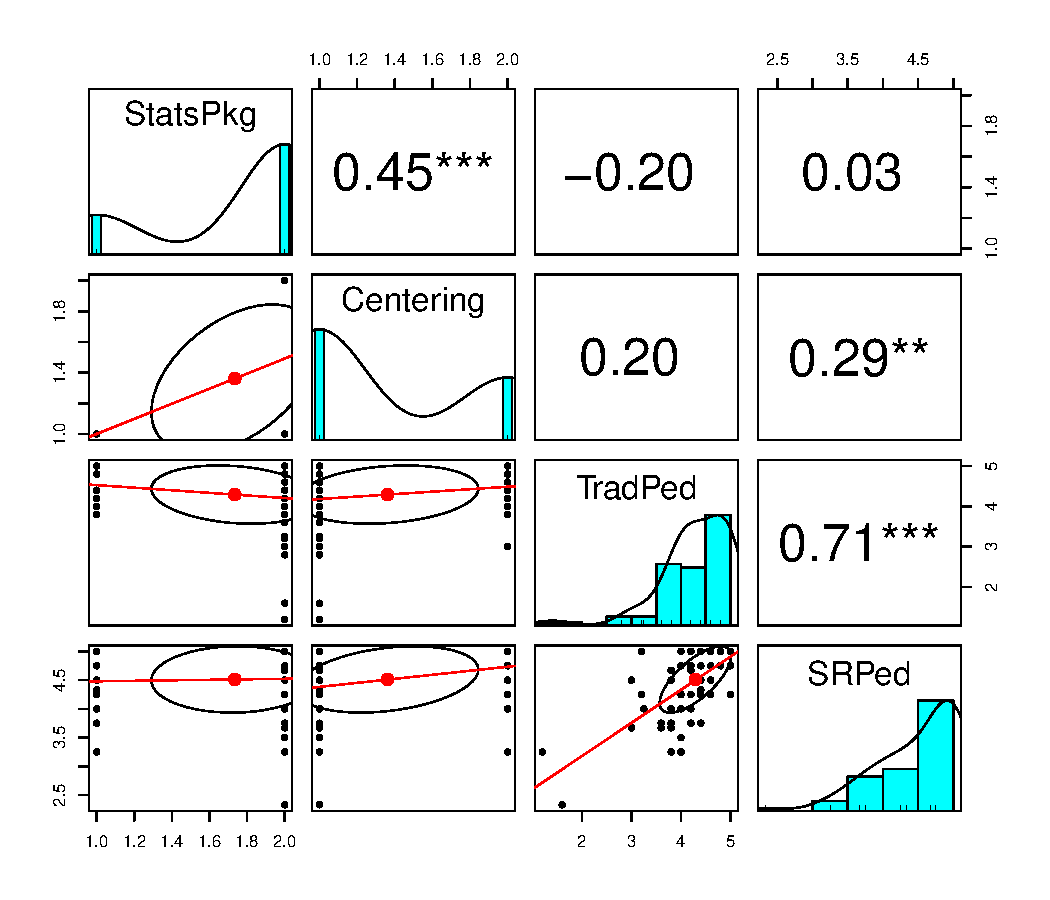
\includegraphics{03-DataDx_files/figure-latex/unnamed-chunk-48-1.pdf}

CUMULATIVE CAPTURE FOR THE APA STYLE WRITE-UP:

\begin{quote}
\begin{quote}
Regarding the distributional characteristics of the data, skew and kurtosis values of the variables fell below the values of 3 (skew) and 10 (kurtosis) that Kline suggests are concerning \citeyearpar{kline_principles_2016}. Results of the Shapiro-Wilk test of normality indicate that our variables assessing the traditional pedagogy (\(W = 0.830, p < 0.001\)) and socially responsive pedagogy (0.818, p \textless{} 0.001) are statistically significantly different than a normal distribution. Inspection of distributions of the variables indicated that both course evaluation variables were negatively skewed, with a large proportion of high scores.
\end{quote}
\end{quote}

\hypertarget{evaluate-multivarite-normality-mahalanobis-test}{%
\subsubsection*{Evaluate multivarite normality (Mahalanobis test)}\label{evaluate-multivarite-normality-mahalanobis-test}}


In more complex models, multivariate normality is probably a more useful analysis. Although I am teaching this evaluation in advance of the formal analysis, as demonstrated in many of \href{https://lhbikos.github.io/ReCenterPsychStats/analysis-of-variance.html}{ReCentering Psych Stats ANOVA chapters}, this can also be assessed by examining the distribution of residuals after the analysis is complete.

Multivariate normality can be assessed with the continuously scaled variables. The code below includes the only two continuously scaled variables. The code simultaneously (a) appends the df with a Mahalanobis value and (b) creates a QQ plot. Dots that stray from the line are the scores that are contributing to multivariate non-normality.

\begin{Shaded}
\begin{Highlighting}[]
\NormalTok{scored}\SpecialCharTok{$}\NormalTok{Mahal }\OtherTok{\textless{}{-}}\NormalTok{ psych}\SpecialCharTok{::}\FunctionTok{outlier}\NormalTok{(scored[}\FunctionTok{c}\NormalTok{(}\StringTok{"TradPed"}\NormalTok{, }\StringTok{"SRPed"}\NormalTok{)])}
\end{Highlighting}
\end{Shaded}

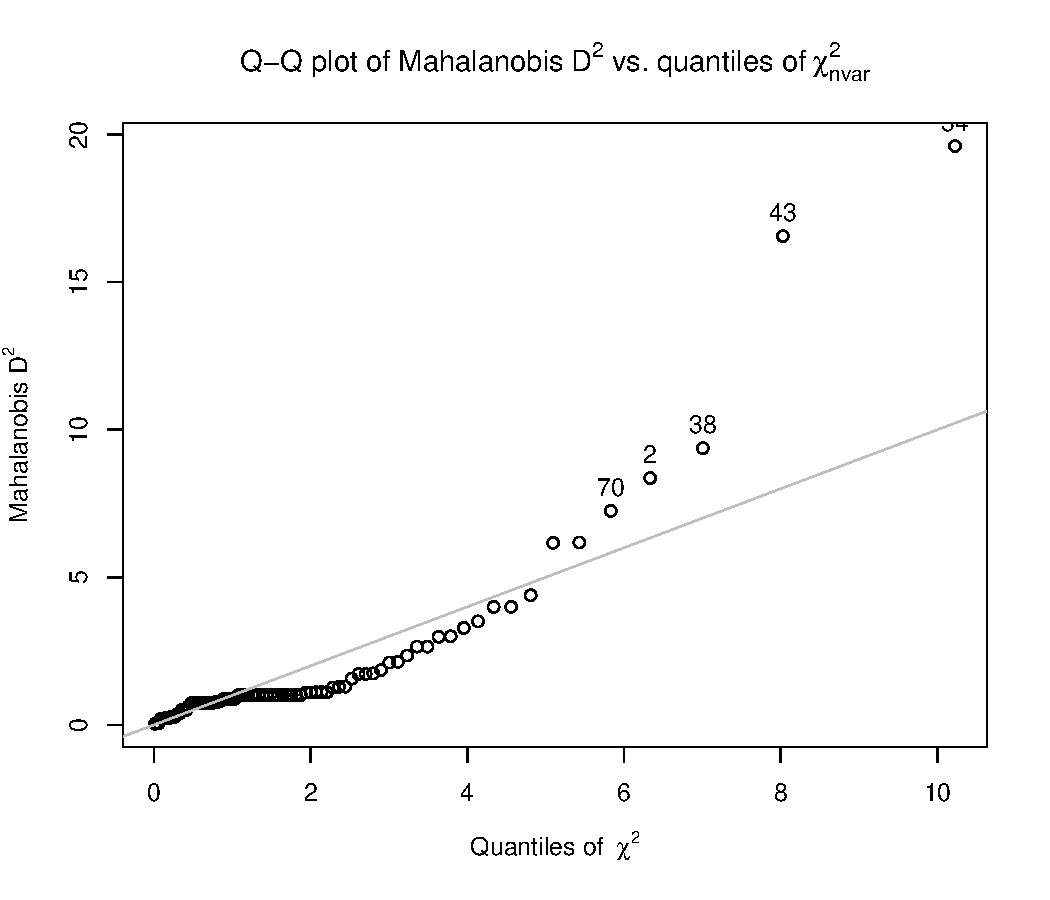
\includegraphics{03-DataDx_files/figure-latex/unnamed-chunk-49-1.pdf}

We can analyze the distributional characteristics of the Mahalanobis values with \emph{psych::describe}. It is possible, then to analyze the Mahalanobis distance values.

\begin{Shaded}
\begin{Highlighting}[]
\NormalTok{psych}\SpecialCharTok{::}\FunctionTok{describe}\NormalTok{(scored}\SpecialCharTok{$}\NormalTok{Mahal)}
\end{Highlighting}
\end{Shaded}

\begin{verbatim}
   vars  n mean   sd median trimmed  mad  min   max range skew kurtosis   se
X1    1 83 1.97 3.12   1.01    1.27 0.42 0.03 19.61 19.58 3.75    15.87 0.34
\end{verbatim}

Using this information we can determine cases that have a Mahalanobis distance values that exceeds three standard deviations around the median. In fact, we can have these noted in a column in the dataframe.

\begin{Shaded}
\begin{Highlighting}[]
\CommentTok{\# creates a variable indicating TRUE or FALSE if an item is an}
\CommentTok{\# outlier}
\NormalTok{scored}\SpecialCharTok{$}\NormalTok{MOutlier }\OtherTok{\textless{}{-}}\NormalTok{ dplyr}\SpecialCharTok{::}\FunctionTok{if\_else}\NormalTok{(scored}\SpecialCharTok{$}\NormalTok{Mahal }\SpecialCharTok{\textgreater{}}\NormalTok{ (}\FunctionTok{median}\NormalTok{(scored}\SpecialCharTok{$}\NormalTok{Mahal) }\SpecialCharTok{+}
\NormalTok{    (}\DecValTok{3} \SpecialCharTok{*} \FunctionTok{sd}\NormalTok{(scored}\SpecialCharTok{$}\NormalTok{Mahal))), }\ConstantTok{TRUE}\NormalTok{, }\ConstantTok{FALSE}\NormalTok{)}

\CommentTok{\# shows us the first 6 rows of the data so we can see the new}
\CommentTok{\# variables (Mahal, MOutlier)}
\FunctionTok{head}\NormalTok{(scored)}
\end{Highlighting}
\end{Shaded}

\begin{verbatim}
  StatsPkg Centering TradPed SRPed     Mahal MOutlier
1     SPSS       Pre     4.2    NA 0.0319020    FALSE
2        R       Pre     2.8    NA 8.3615550    FALSE
3        R        Re     3.8   4.5 0.8702516    FALSE
4        R        Re     5.0   5.0 1.0087776    FALSE
5        R        Re     4.8   5.0 0.7363631    FALSE
6        R        Re     4.0   5.0 2.6509906    FALSE
\end{verbatim}

\begin{Shaded}
\begin{Highlighting}[]
\FunctionTok{library}\NormalTok{(tidyverse)}
\CommentTok{\# counts frequency TRUE and FALSE indicating outlier or not}
\NormalTok{OutlierCount }\OtherTok{\textless{}{-}}\NormalTok{ scored }\SpecialCharTok{\%\textgreater{}\%}
\NormalTok{    dplyr}\SpecialCharTok{::}\FunctionTok{count}\NormalTok{(MOutlier)}

\CommentTok{\# calculating how many outliers a slightly different way}
\FunctionTok{nrow}\NormalTok{(scored) }\SpecialCharTok{{-}}\NormalTok{ OutlierCount}
\end{Highlighting}
\end{Shaded}

\begin{verbatim}
  MOutlier  n
1       83  2
2       82 81
\end{verbatim}

When we identify outliers we often ask if we should delete them or transform the data. A general rule of thumb is to look for ``jumps'' in the Mahalanobis distance values. If they are progressing steadily and there is no ``jump,'' researchers will often retain the outliers.

In this case, I do see a jump. When I sort the df on Mahal values, the jump from 9.37 to 16.56 is much different than the more gradual increase in values that precedes it. Therefore, I think I will delete cases with Mahalanobis values greater than 10 (a number I ``just picked'').

\begin{Shaded}
\begin{Highlighting}[]
\NormalTok{scored }\OtherTok{\textless{}{-}}\NormalTok{ dplyr}\SpecialCharTok{::}\FunctionTok{filter}\NormalTok{(scored, Mahal }\SpecialCharTok{\textless{}} \StringTok{"10"}\NormalTok{)}
\end{Highlighting}
\end{Shaded}

\begin{quote}
\begin{quote}
We evaluated multivariate normality with the Mahalanobis distance test. Specifically, we used the \emph{psych::outlier()} function and included both continuous variables in the calculation. Our visual inspection of the Q-Q plot suggested that the plotted line strayed from the straight line as the quantiles increased. Additionally, we appended the Mahalanobis distance scores as a variable to the data. Analyzing this variable, we found that 2 cases exceed three standard deviations beyond the median. Because there was a substantial ``jump'' between the non-outliers and these two variables we chose to delete them.
\end{quote}
\end{quote}

\hypertarget{represent-your-work-in-an-apa-style-write-up-added-to-the-writeup-in-the-previous-chapter-1}{%
\subsubsection*{Represent your work in an APA-style write-up (added to the writeup in the previous chapter)}\label{represent-your-work-in-an-apa-style-write-up-added-to-the-writeup-in-the-previous-chapter-1}}


\begin{quote}
\begin{quote}
This is a secondary analysis of data involved in a more comprehensive dataset that included students taking multiple statistics courses (\emph{N} = 310). Having retrieved this data from a repository in the Open Science Framework, only those who consented to participation in the study were included. Data used in these analyses were 84 students who completed the multivariate clas.
\end{quote}
\end{quote}

\begin{quote}
\begin{quote}
Available item analysis (AIA; \citep{parent_handling_2013}) is a strategy for managing missing data that uses available data for analysis and excludes cases with missing data points only for analyses in which the data points would be directly involved. Parent (2013) suggested that AIA is equivalent to more complex methods (e.g., multiple imputation) across a number of variations of sample size, magnitude of associations among items, and degree of missingness. Thus, we utilized Parent's recommendations to guide our approach to managing missing data. Missing data analyses were conducted with tools in base R as well as the R packages, \emph{psych} (v. 2.3.6) and \emph{mice} (v. 3.16.0).
\end{quote}
\end{quote}

\begin{quote}
\begin{quote}
Across cases that were deemed eligible on the basis of the inclusion/exclusion criteria, missingness ranged from 0 to 100\%. Across the dataset, 3.86\% of cells had missing data and 87.88\% of cases had nonmissing data.
\end{quote}
\end{quote}

\begin{quote}
\begin{quote}
Across the 84 cases for which the scoring protocol was applied, missingness ranged from 0 to 67\%. After eliminating cases with greater than 20\% missing, the dataset analyzed included 83 cases. In this dataset we had less than 1\% (0.60\%) missing across the df; 98\% of the rows had nonmissing data.
\end{quote}
\end{quote}

\begin{quote}
\begin{quote}
Regarding the distributional characteristics of the data, skew and kurtosis values of the variables fell below the values of 3 (skew) and 10 (kurtosis) that Kline suggests are concerning \citeyearpar{kline_principles_2016}. Results of the Shapiro-Wilk test of normality indicate that our variables assessing the traditional pedagogy (\(W = 0.830, p < 0.001\)) and socially responsive pedagogy (0.818, p \textless{} 0.001) are statistically significantly different than a normal distribution. Inspection of distributions of the variables indicated that both course evaluation variables were negatively skewed, with a large proportion of high scores.
\end{quote}
\end{quote}

\begin{quote}
\begin{quote}
We evaluated multivariate normality with the Mahalanobis distance test. Specifically, we used the \emph{psych::outlier()} function and included both continuous variables in the calculation. Our visual inspection of the Q-Q plot suggested that the plotted line strayed from the straight line as the quantiles increased. Additionally, we appended the Mahalanobis distance scores as a variable to the data. Analyzing this variable, we found that 2 cases exceed three standard deviations beyond the median. Because there was a substantial ``jump'' between the non-outliers and these two variables we chose to delete them.
\end{quote}
\end{quote}

\hypertarget{conduct-a-quick-analysis-e.g.-regression-anova-including-at-least-three-variables}{%
\subsubsection*{Conduct a quick analysis (e.g., regression, ANOVA) including at least three variables}\label{conduct-a-quick-analysis-e.g.-regression-anova-including-at-least-three-variables}}


\begin{Shaded}
\begin{Highlighting}[]
\NormalTok{SRPed\_fit }\OtherTok{\textless{}{-}} \FunctionTok{lm}\NormalTok{(SRPed }\SpecialCharTok{\textasciitilde{}}\NormalTok{ StatsPkg }\SpecialCharTok{+}\NormalTok{ Centering }\SpecialCharTok{+}\NormalTok{ TradPed, }\AttributeTok{data =}\NormalTok{ scored)}
\FunctionTok{summary}\NormalTok{(SRPed\_fit)}
\end{Highlighting}
\end{Shaded}

\begin{verbatim}

Call:
lm(formula = SRPed ~ StatsPkg + Centering + TradPed, data = scored)

Residuals:
     Min       1Q   Median       3Q      Max 
-0.56099 -0.14406  0.01551  0.10594  0.46498 

Coefficients:
            Estimate Std. Error t value          Pr(>|t|)    
(Intercept)  1.46330    0.34441   4.249 0.000077464849487 ***
StatsPkgR    0.13251    0.08056   1.645             0.105    
CenteringRe  0.05666    0.07423   0.763             0.448    
TradPed      0.68663    0.07365   9.323 0.000000000000332 ***
---
Signif. codes:  0 '***' 0.001 '**' 0.01 '*' 0.05 '.' 0.1 ' ' 1

Residual standard error: 0.2433 on 59 degrees of freedom
  (1 observation deleted due to missingness)
Multiple R-squared:  0.6167,    Adjusted R-squared:  0.5972 
F-statistic: 31.64 on 3 and 59 DF,  p-value: 0.000000000002547
\end{verbatim}

\hypertarget{results-2}{%
\subsection{Results}\label{results-2}}

\begin{quote}
\begin{quote}
Results of a multiple regression predicting the socially responsive course evaluation ratings indicated that neither the transition from SPSS to R (\(B = 0.133, p = 0.105\)) nor the transition to an explicitly recentered curriculum (\(B = 0.057, p = 0.448) led to statistically significant diferences. In contrast, traditional pedagogy had a strong, positive effect on evaluations of socially responsive pedagogy (\)B = 0.686, p \textless{} 0.001). The model accounted for 62\% of the variance and was statistically significant (\(p , 0.001\)). Means, standard deviations, and correlations among variables are presented in Table 1; results of the regression model are presented in Table 2.
\end{quote}
\end{quote}

\begin{Shaded}
\begin{Highlighting}[]
\NormalTok{apaTables}\SpecialCharTok{::}\FunctionTok{apa.cor.table}\NormalTok{(scored[}\FunctionTok{c}\NormalTok{(}\StringTok{"SRPed"}\NormalTok{, }\StringTok{"StatsPkg"}\NormalTok{, }\StringTok{"Centering"}\NormalTok{, }\StringTok{"TradPed"}\NormalTok{)],}
    \AttributeTok{table.number =} \DecValTok{1}\NormalTok{, }\AttributeTok{show.sig.stars =} \ConstantTok{TRUE}\NormalTok{, }\AttributeTok{filename =} \StringTok{"Table1\_\_DataDx\_HW.doc"}\NormalTok{)}
\end{Highlighting}
\end{Shaded}

\begin{verbatim}


Table 1 

Means, standard deviations, and correlations with confidence intervals
 

  Variable   M    SD   1         
  1. SRPed   4.69 0.38           
                                 
  2. TradPed 4.53 0.43 .76**     
                       [.63, .85]
                                 

Note. M and SD are used to represent mean and standard deviation, respectively.
Values in square brackets indicate the 95% confidence interval.
The confidence interval is a plausible range of population correlations 
that could have caused the sample correlation (Cumming, 2014).
 * indicates p < .05. ** indicates p < .01.
 
\end{verbatim}

\begin{Shaded}
\begin{Highlighting}[]
\NormalTok{apaTables}\SpecialCharTok{::}\FunctionTok{apa.reg.table}\NormalTok{(SRPed\_fit, }\AttributeTok{table.number =} \DecValTok{2}\NormalTok{, }\AttributeTok{filename =} \StringTok{"SRPed\_table.doc"}\NormalTok{)}
\end{Highlighting}
\end{Shaded}

\begin{verbatim}


Table 2 

Regression results using SRPed as the criterion
 

   Predictor      b      b_95%_CI sr2  sr2_95%_CI             Fit
 (Intercept) 1.46**  [0.77, 2.15]                                
   StatsPkgR   0.13 [-0.03, 0.29] .02 [-.02, .06]                
 CenteringRe   0.06 [-0.09, 0.21] .00 [-.02, .02]                
     TradPed 0.69**  [0.54, 0.83] .56  [.40, .73]                
                                                      R2 = .617**
                                                  95% CI[.43,.70]
                                                                 

Note. A significant b-weight indicates the semi-partial correlation is also significant.
b represents unstandardized regression weights. 
sr2 represents the semi-partial correlation squared.
Square brackets are used to enclose the lower and upper limits of a confidence interval.
* indicates p < .05. ** indicates p < .01.
 
\end{verbatim}

\hypertarget{multimp}{%
\chapter{Multiple Imputation (A Brief Demo)}\label{multimp}}

\href{https://spu.hosted.panopto.com/Panopto/Pages/Viewer.aspx?pid=94d59efe-3f02-4c65-b068-ad01003e09a9}{Screencasted Lecture Link}

Multiple imputation is a tool for managing missing data that works with the whole raw data file to impute values for missing data for \emph{multiple sets} (e.g., 5-20) of the raw data. Those multiple sets are considered together in analyses (such as regression) and interpretation is made on the pooled results. Much has been written about multiple imputation and, if used, should be done with many considerations. This chapter is intended as a brief introduction. In this chapter, I demonstrate the use of multiple imputation with the data from the \href{https://spupsych.az1.qualtrics.com/jfe/form/SV_b2cClqAlLGQ6nLU}{Rate-a-Recent-Course: A ReCentering Psych Stats Exercise} that has served as the research vignette for the first few chapters of this OER.

\hypertarget{navigating-this-lesson-3}{%
\section{Navigating this Lesson}\label{navigating-this-lesson-3}}

There is about one hour of lecture. If you work through the materials with me it would be good to add another hour (to an hour-and-a-half).

While the majority of R objects and data you will need are created within the R script that sources the chapter, there are a few that cannot be created from within the R framework. Additionally, sometimes links fail. All original materials are provided at the \href{https://github.com/lhbikos/ReC_MultivModel}{Github site} that hosts the book. More detailed guidelines for ways to access all these materials are provided in the OER's \protect\hyperlink{ReCintro}{introduction}

\hypertarget{learning-objectives-3}{%
\subsection{Learning Objectives}\label{learning-objectives-3}}

Learning objectives from this lecture include the following:

\begin{itemize}
\tightlist
\item
  Describe circumstances under which multiple imputation would be appropriate
\item
  List and define the stages in multiple imputation.
\item
  Apply multiple imputation to a dataset that has missingness
\item
  Interpret results from a simple regression that uses multiple imputation
\item
  Articulate how multiple imputation fits into the workflow for scrubbing and scoring data.
\item
  Write up the results of an the process of imputation from raw data through analyzing a simple regression (or similar) analysis.
\end{itemize}

\hypertarget{planning-for-practice-3}{%
\subsection{Planning for Practice}\label{planning-for-practice-3}}

The suggestions for practice are a continuation from the three prior chapters. If you have completed one or more of those assignments, you should have worked through the steps in preparing a data set and evaluating its appropriateness for the planned, statistical, analysis. This chapter takes a deviation from the AIA \citep{parent_handling_2013} approach that was the focus of the first few chapters in that we used multiple imputation as the approach for managing missingness. Options, of graded complexity, for practice include:

\begin{itemize}
\tightlist
\item
  Repeating the steps in the chapter with the most recent data from the Rate-A-Recent-Course survey; differences will be in the number of people who have completed the survey since the chapter was written.
\item
  Use the dataset that is the source of the chapter, but score a different set of items that you choose.
\item
  Begin with raw data to which you have access.
\end{itemize}

\hypertarget{readings-resources-3}{%
\subsection{Readings \& Resources}\label{readings-resources-3}}

In preparing this chapter, I drew heavily from the following resource(s). Other resources are cited (when possible, linked) in the text with complete citations in the reference list.

\begin{itemize}
\tightlist
\item
  Enders, C. K. (2017). Multiple imputation as a flexible tool for missing data handling in clinical research. \emph{Behaviour Research and Therapy}, 98, 4--18.

  \begin{itemize}
  \tightlist
  \item
    Craig Enders is a leading expert in the analysis and management of missing data. This article is useful in describing multiple imputation as a method for managing missingness.
  \end{itemize}
\item
  Katitas, A. (2019). Getting Started with Multiple Imputation in R. University of Virginia Library: Research Data Services + Sciences. \url{https://library.virginia.edu/data/articles/getting-started-with-multiple-imputation-in-r}

  \begin{itemize}
  \tightlist
  \item
    Tutorial for conducting multiple imputation in R.
  \end{itemize}
\item
  Kline Ch4, Data Preparation \& Psychometrics Review (pp.~72/Outliers - 88/Modern Methods)
\item
  Kline's chapter is my ``go-to'' for making decisions about preparing data for analysis.
\end{itemize}

\hypertarget{packages-3}{%
\subsection{Packages}\label{packages-3}}

The script below will (a) check to see if the following packages are installed on your computer and, if not (b) install them.

\begin{Shaded}
\begin{Highlighting}[]
\CommentTok{\# will install the package if not already installed}
\ControlFlowTok{if}\NormalTok{ (}\SpecialCharTok{!}\FunctionTok{require}\NormalTok{(qualtRics)) \{}
    \FunctionTok{install.packages}\NormalTok{(}\StringTok{"qualtRics"}\NormalTok{)}
\NormalTok{\}}
\ControlFlowTok{if}\NormalTok{ (}\SpecialCharTok{!}\FunctionTok{require}\NormalTok{(psych)) \{}
    \FunctionTok{install.packages}\NormalTok{(}\StringTok{"psych"}\NormalTok{)}
\NormalTok{\}}
\ControlFlowTok{if}\NormalTok{ (}\SpecialCharTok{!}\FunctionTok{require}\NormalTok{(dplyr)) \{}
    \FunctionTok{install.packages}\NormalTok{(}\StringTok{"dplyr"}\NormalTok{)}
\NormalTok{\}}
\ControlFlowTok{if}\NormalTok{ (}\SpecialCharTok{!}\FunctionTok{require}\NormalTok{(mice)) \{}
    \FunctionTok{install.packages}\NormalTok{(}\StringTok{"mice"}\NormalTok{)}
\NormalTok{\}}
\end{Highlighting}
\end{Shaded}

\hypertarget{workflow-for-multiple-imputation}{%
\section{Workflow for Multiple Imputation}\label{workflow-for-multiple-imputation}}

The following is a proposed workflow for preparing data for analysis.

\begin{figure}
\centering
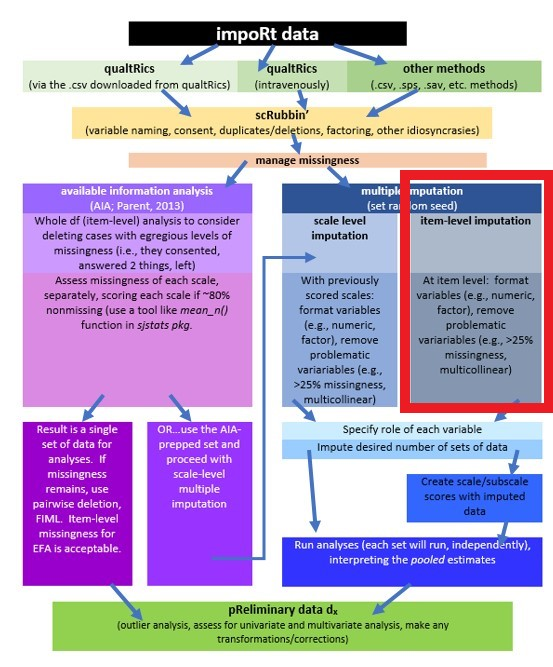
\includegraphics{images/Ch05/scrubscore_mimp_itemlvl.jpg}
\caption{An image of a workflow for scrubbing and scoring data.}
\end{figure}

In this lecture we are working on the right side of the flowchart in the multiple imputation (blue) section. Within it, there are two options, each with a slightly different set of options.

\begin{itemize}
\tightlist
\item
  imputing at the item level

  \begin{itemize}
  \tightlist
  \item
    in this case, scales/subscales are scored after the item-level imputation
  \end{itemize}
\item
  imputating at the scale level

  \begin{itemize}
  \tightlist
  \item
    in this case, scales/subscales are scored prior to the imputation; likely using some of the same criteria as identified in the scoring chapter (i.e., scoring if 75-80\% of data are non-missing). Multiple imputation, then, is used to estimate the remaining, missing values.
  \end{itemize}
\end{itemize}

Whichever approach is used, the imputed variables (multiple sets) are used in a \emph{pooled analysis} and results are interpreted from that analysis.

\hypertarget{research-vignette-3}{%
\section{Research Vignette}\label{research-vignette-3}}

The research vignette comes from the survey titled, \href{https://spupsych.az1.qualtrics.com/jfe/form/SV_b2cClqAlLGQ6nLU}{Rate-a-Recent-Course: A ReCentering Psych Stats Exercise} and is explained in the \protect\hyperlink{scrub}{scrubbing chapter}. In the \protect\hyperlink{score}{scoring chapter} we prepared four variables for analysis. In the \protect\hyperlink{DataDx}{data diagnostics chapter} we assessed the quality of the variables and conducted the multiple regression described below. Details for these are in our \href{./Rate-a-Course_Codebook.pdf}{codebook}.

Let's quickly review the variables in our model:

\begin{itemize}
\tightlist
\item
  Perceived Campus Climate for Black Students includes 6 items, one of which was reverse scored. This scale was adapted from Szymanski et al.'s \citeyearpar{szymanski_perceptions_2020} Campus Climate for LGBTQ students. It has not been evaluated for use with other groups. The Szymanski et al.~analysis suggested that it could be used as a total scale score, or divided into three items each that assess

  \begin{itemize}
  \tightlist
  \item
    College response to LGBTQ students (items 6, 4, 1)
  \item
    LGBTQ stigma (items 3, 2, 5)
  \end{itemize}
\item
  Sense of Belonging includes 3 items. This is a subscale from Bollen and Hoyle's \citeyearpar{bollen_perceived_1990} Perceived Cohesion Scale. There are no items on this scale that require reversing.
\item
  Percent of Black classmates is a single item that asked respondents to estimate the proportion of students in various racial categories
\item
  Percent of BIPOC instructional staff, similarly, asked respondents to identify the racial category of each member of their instructional staff
\end{itemize}

As we noted in the \protect\hyperlink{scrub}{scrubbing chapter}, our design has notable limitations. Briefly, (a) owing to the open source aspect of the data we do not ask about the demographic characteristics of the respondent; (b) the items that ask respondents to \emph{guess} the identities of the instructional staff and to place them in broad categories, (c) we do not provide a ``write-in'' a response. We made these decisions after extensive conversation with stakeholders. The primary reason for these decisions was to prevent potential harm (a) to respondents who could be identified if/when the revealed private information in this open-source survey, and (b) trolls who would write inappropriate or harmful comments.

As I think about ``how these variables go together'' (which is often where I start in planning a study), I suspect parallel mediation. That is the perception of campus climate for Black students would be predicted by the respondent's sense of belonging, mediated in separate paths through the proportion of classmates who are Black and the proportion of BIPOC instructional staff.

\emph{I would like to assess the model by having the instructional staff variable to be the \%Black instructional staff. At the time that this lecture is being prepared, there is not sufficient Black representation in the instructional staff to model this.}

\begin{figure}
\centering
\includegraphics{images/Ch04/BlStuMed.jpg}
\caption{An image of the statistical model for which we are preparing data.}
\end{figure}

As in the \protect\hyperlink{DataDx}{data diagnostic chapter}, I will conclude this chapter by conducting a statistical analysis with the multiply imputed data. Because parallel mediation can be complicated (I teach it in a later chapter), I will demonstrate use of our prepared variables with a simple multiple regression.

\begin{figure}
\centering
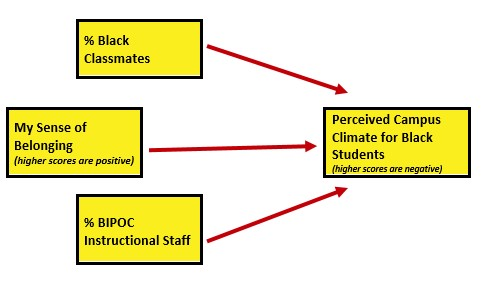
\includegraphics{images/Ch04/BlStuRegression.jpg}
\caption{An image of the statistical model for which we are preparing data.}
\end{figure}

\hypertarget{multiple-imputation-a-super-brief-review}{%
\section{Multiple Imputation -- a Super Brief Review}\label{multiple-imputation-a-super-brief-review}}

Multiple imputation is complex. Numerous quantitative psychologists had critiqued it and provided numerous cautions and guidelines for its use \citep{enders_applied_2010, enders_multiple_2017, little_missing_2008, little_statistical_2002}. In brief,

\hypertarget{steps-in-multiple-imputation}{%
\subsection{Steps in Multiple Imputation}\label{steps-in-multiple-imputation}}

\begin{itemize}
\tightlist
\item
  Multiple imputation starts with a raw data file.

  \begin{itemize}
  \tightlist
  \item
    Multiple imputation assumes that data are MAR (remember, MCAR is the more prestigious one). This means that researchers assume that missing values can be replaced by predictions derived from the observable portion of the dataset.\\
  \end{itemize}
\item
  Multiple datasets (often 5 to 20) are created where missing values are replaced via a randomized process (so the same missing value {[}item 4 for person A{]} will likely have different values for each dataset).
\item
  The desired analysis is conducted simultaneously/separately for each of the imputed sets (so if you imputed 5 sets and wanted a linear regression, you get 5 linear regressions).\\
\item
  A \emph{pooled analysis} uses the point estimates and the standard errors to provide a single result that represents the analysis.
\end{itemize}

In a web-hosted guide from the University of Virginia Library, Katitas \citeyearpar{katitas_getting_2019} provided a user-friendly review and example of using tools in R in a multiple imputation. Katitas' figure is a useful conceptual tool in understanding how multiple imputation works. \emph{This figure is my recreation of Katitas' original.}

\begin{figure}
\centering
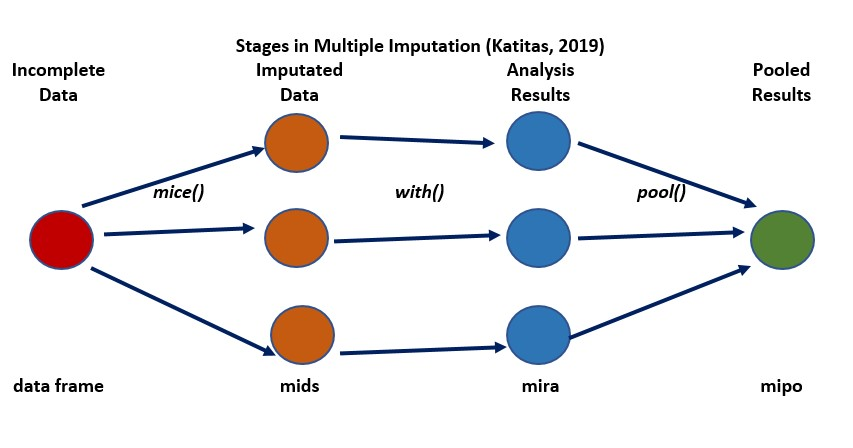
\includegraphics{images/Ch05/KatitasMimpFig.jpg}
\caption{An image adapted from the Katitas multiple imputation guide showing the four stages of multiple imputation.}
\end{figure}

\begin{itemize}
\tightlist
\item
  the dataframe with missing data is the single place we start
\item
  we intervene with a package like \emph{mice()} to
\item
  impute multiple sets of data (filling in the missing variables with different values that are a product of their conditional distribution and an element of ``random'');

  \begin{itemize}
  \tightlist
  \item
    ``mids'' (``multiply imputed dataset'') is an object class where the completed datasets are stored.
  \end{itemize}
\item
  the ``with\_mids'' command allows OLS regression to be run, as many times as we have imputed datasets (in this figure, 3X). It produces different regression coefficients for each datset
\item
  the ``pool'' command pools together the multiple coefficients taking into consideration the value of the coefficients,the standard errors, and the variance of the missing value parameter across the samples.
\end{itemize}

\hypertarget{statistical-approaches-to-multiple-imputation}{%
\subsection{Statistical Approaches to Multiple Imputation}\label{statistical-approaches-to-multiple-imputation}}

\textbf{Joint multivariate normal distribution multiple imputation} assumes that the observed data follow a multivariate normal distribution. The algorithm used draws from this assumed distribution. A drawback is that if the data do not follow a multivariate normal distribution, the imputed values are incorrect. \emph{Amelia} and \emph{norm} packages use this approach.

\textbf{Conditional multiple imputation} is an iterative procedure, modeling the conditional distribution of a certain variable given the other variables. In this way the distribution is assumed for each variable, rather than or the entire dataset. \emph{mice} uses this approach.

\emph{mice}: multivariate imputation by chained equations

\hypertarget{working-the-problem-2}{%
\section{Working the Problem}\label{working-the-problem-2}}

Katitas \citeyearpar{katitas_getting_2019} claims that it is best to impute the data in its rawest form possible because any change would be taking it away from its original distribution. There are debates about how many variables to include in an imputation. Some authors would suggest that researchers include everything that was collected. Others (like me) will trim the dataset to include (a) the variables included in the model, plus (b) auxiliary variables (i.e., variables not in the model, but that are sufficiently non-missing and will provide additional information to the data).

In our case we will want:

Item for the variables represented in our model

\begin{itemize}
\tightlist
\item
  the item level responses to the scales/subscales

  \begin{itemize}
  \tightlist
  \item
    respondents' sense of belonging to campus (3 items)
  \item
    respondents' rating of campus climate for Black students (6 items)
  \end{itemize}
\item
  proportion of BIPOC instructional staff
\item
  proportion of classmates who are Black
\end{itemize}

Auxiliary variables -- let's choose four. One will be the format of the course. Three items will be from the course evaluation.

\begin{itemize}
\tightlist
\item
  format, whether the course was taught in-person, a blend, or virtual
\item
  cEval\_1, ``Course material was presented clearly''
\item
  cEval\_13, ``Where applicable, issues were considered from multiple perspectives''
\item
  cEval\_19, ``My understanding of the subject matter increased over the span of the course''
\end{itemize}

\hypertarget{selecting-and-formatting-variables}{%
\subsection{Selecting and Formatting Variables}\label{selecting-and-formatting-variables}}

There are some guidelines for selecting and formatting variables for imputation.

\begin{itemize}
\tightlist
\item
  Variables should be in their \emph{most natural} state
\item
  Redundant or too highly correlated variables should not be included

  \begin{itemize}
  \tightlist
  \item
    If you reverse coded a variable (we haven't yet), that's ok, but if you have already reverse-coded, then exclude the original variable
  \item
    Redundant variables (or multicollinear variables) may cause the multiple imputation process to cease
  \item
    Violation of this also provides clues for troubleshooting
  \end{itemize}
\item
  Exclude variables with more than 25\% missing
\end{itemize}

To make this as realistic as possible. Let's start with our very raw data. The \protect\hyperlink{scrub}{Scrubbing chapter} provides greater detail on importing data directly from Qualtrics. If you have worked the lessons, consecutively, you know that data can be added to this survey at any time. So that the values in the chapter are consistent, I will use the datafiles that I immediately saved when I conducted the analysis at the time I last updated the chapter.

Please download the .rds or .csv file from \href{https://github.com/lhbikos/ReC_MultivModel}{MultivModel GitHub} site. Please the file in the same folder as your .rmd file. As always, I prefer working with .rds files.

\begin{Shaded}
\begin{Highlighting}[]
\NormalTok{QTRX\_df2 }\OtherTok{\textless{}{-}} \FunctionTok{readRDS}\NormalTok{(}\StringTok{"QTRX\_df230902b.rds"}\NormalTok{)}
\CommentTok{\# QTRX\_df \textless{}{-} read.csv(\textquotesingle{}QTRX\_df230902b.csv\textquotesingle{}, header = TRUE)}
\end{Highlighting}
\end{Shaded}

Next, I apply inclusion/exclusion criteria. As described in the \protect\hyperlink{scrub}{Scrubbing chapter} this includes:

\begin{itemize}
\tightlist
\item
  excluding all \emph{previews}
\item
  including only those who consented
\item
  including only those whose rated course was offered by a U.S. institution
\end{itemize}

\begin{Shaded}
\begin{Highlighting}[]
\FunctionTok{library}\NormalTok{(tidyverse)}
\NormalTok{QTRX\_df2 }\OtherTok{\textless{}{-}}\NormalTok{ dplyr}\SpecialCharTok{::}\FunctionTok{filter}\NormalTok{(QTRX\_df2, DistributionChannel }\SpecialCharTok{!=} \StringTok{"preview"}\NormalTok{)}
\NormalTok{QTRX\_df2 }\OtherTok{\textless{}{-}}\NormalTok{ dplyr}\SpecialCharTok{::}\FunctionTok{filter}\NormalTok{(QTRX\_df2, Consent }\SpecialCharTok{==} \DecValTok{1}\NormalTok{)}
\NormalTok{QTRX\_df2 }\OtherTok{\textless{}{-}}\NormalTok{ dplyr}\SpecialCharTok{::}\FunctionTok{filter}\NormalTok{(QTRX\_df2, USinst }\SpecialCharTok{==} \DecValTok{0}\NormalTok{)}
\end{Highlighting}
\end{Shaded}

Preparing the data also meant renaming some variables that started with numbers (a hassle in R). I also renamed variables on the Campus Climate scale so that we know to which subscale they belong.

\begin{Shaded}
\begin{Highlighting}[]
\CommentTok{\# renaming variables that started with numbers}
\NormalTok{QTRX\_df2 }\OtherTok{\textless{}{-}}\NormalTok{ dplyr}\SpecialCharTok{::}\FunctionTok{rename}\NormalTok{(QTRX\_df2, }\AttributeTok{iRace1 =} \StringTok{"1\_iRace"}\NormalTok{, }\AttributeTok{iRace2 =} \StringTok{"2\_iRace"}\NormalTok{,}
    \AttributeTok{iRace3 =} \StringTok{"3\_iRace"}\NormalTok{, }\AttributeTok{iRace4 =} \StringTok{"4\_iRace"}\NormalTok{, }\AttributeTok{iRace5 =} \StringTok{"5\_iRace"}\NormalTok{, }\AttributeTok{iRace6 =} \StringTok{"6\_iRace"}\NormalTok{,}
    \AttributeTok{iRace7 =} \StringTok{"7\_iRace"}\NormalTok{, }\AttributeTok{iRace8 =} \StringTok{"8\_iRace"}\NormalTok{, }\AttributeTok{iRace9 =} \StringTok{"9\_iRace"}\NormalTok{, }\AttributeTok{iRace10 =} \StringTok{"10\_iRace"}\NormalTok{)}
\CommentTok{\# renaming variables from the identification of classmates}
\NormalTok{QTRX\_df2 }\OtherTok{\textless{}{-}}\NormalTok{ dplyr}\SpecialCharTok{::}\FunctionTok{rename}\NormalTok{(QTRX\_df2, }\AttributeTok{cmBiMulti =}\NormalTok{ Race\_10, }\AttributeTok{cmBlack =}\NormalTok{ Race\_1,}
    \AttributeTok{cmNBPoC =}\NormalTok{ Race\_7, }\AttributeTok{cmWhite =}\NormalTok{ Race\_8, }\AttributeTok{cmUnsure =}\NormalTok{ Race\_2)}
\end{Highlighting}
\end{Shaded}

The Qualtrics download does not include an ID number. Because new variables are always appended to the end of the df, we also include code to make this the first column.

\begin{Shaded}
\begin{Highlighting}[]
\NormalTok{QTRX\_df2 }\OtherTok{\textless{}{-}}\NormalTok{ QTRX\_df2 }\SpecialCharTok{\%\textgreater{}\%}
\NormalTok{    dplyr}\SpecialCharTok{::}\FunctionTok{mutate}\NormalTok{(}\AttributeTok{ID =} \FunctionTok{row\_number}\NormalTok{())}
\CommentTok{\# moving the ID number to the first column; requires}
\NormalTok{QTRX\_df2 }\OtherTok{\textless{}{-}}\NormalTok{ QTRX\_df2 }\SpecialCharTok{\%\textgreater{}\%}
\NormalTok{    dplyr}\SpecialCharTok{::}\FunctionTok{select}\NormalTok{(ID, }\FunctionTok{everything}\NormalTok{())}
\end{Highlighting}
\end{Shaded}

Because this huge df is cumbersome to work with, let's downsize it to be closer to the size we will work with in the imputation

\begin{Shaded}
\begin{Highlighting}[]
\NormalTok{mimp\_df }\OtherTok{\textless{}{-}}\NormalTok{ dplyr}\SpecialCharTok{::}\FunctionTok{select}\NormalTok{(QTRX\_df2, ID, iRace1, iRace2, iRace3, iRace4,}
\NormalTok{    iRace5, iRace6, iRace7, iRace8, iRace9, iRace10, cmBiMulti, cmBlack,}
\NormalTok{    cmNBPoC, cmWhite, cmUnsure, Belong\_1}\SpecialCharTok{:}\NormalTok{Belong\_3, Blst\_1}\SpecialCharTok{:}\NormalTok{Blst\_6, cEval\_1,}
\NormalTok{    cEval\_13, cEval\_19, format)}
\CommentTok{\# glimpse(mimp\_df)}
\FunctionTok{head}\NormalTok{(mimp\_df)}
\end{Highlighting}
\end{Shaded}

\begin{verbatim}
# A tibble: 6 x 29
     ID iRace1 iRace2 iRace3 iRace4 iRace5 iRace6 iRace7 iRace8 iRace9 iRace10
  <int>  <dbl>  <dbl>  <dbl>  <dbl> <lgl>  <lgl>  <lgl>  <lgl>  <lgl>  <lgl>  
1     1      3      1      3     NA NA     NA     NA     NA     NA     NA     
2     2      3     NA     NA     NA NA     NA     NA     NA     NA     NA     
3     3      3      1     NA     NA NA     NA     NA     NA     NA     NA     
4     4      3      1      3     NA NA     NA     NA     NA     NA     NA     
5     5      1     NA     NA     NA NA     NA     NA     NA     NA     NA     
6     6      3     NA     NA     NA NA     NA     NA     NA     NA     NA     
# i 18 more variables: cmBiMulti <dbl>, cmBlack <dbl>, cmNBPoC <dbl>,
#   cmWhite <dbl>, cmUnsure <dbl>, Belong_1 <dbl>, Belong_2 <dbl>,
#   Belong_3 <dbl>, Blst_1 <dbl>, Blst_2 <dbl>, Blst_3 <dbl>, Blst_4 <dbl>,
#   Blst_5 <dbl>, Blst_6 <dbl>, cEval_1 <dbl>, cEval_13 <dbl>, cEval_19 <dbl>,
#   format <dbl>
\end{verbatim}

\hypertarget{creating-composite-variables}{%
\subsection{Creating Composite Variables}\label{creating-composite-variables}}

Qualtrics imports many of the categorical variables as numbers. R often reads them numerically (integers or numbers). If they are directly converted to factors, R will sometimes collapse. In this example, if there is a race that is not represented (e.g., 2 for BiMulti), when the numbers are changed to factors, R will assume it's ordered and will change up the numbers. Therefore, it is ESSENTIAL to check (again and again ad nauseum) to ensure that your variables are recoding in a manner you understand.

\begin{Shaded}
\begin{Highlighting}[]
\NormalTok{mimp\_df}\SpecialCharTok{$}\NormalTok{iRace1 }\OtherTok{=} \FunctionTok{factor}\NormalTok{(mimp\_df}\SpecialCharTok{$}\NormalTok{iRace1, }\AttributeTok{levels =} \FunctionTok{c}\NormalTok{(}\DecValTok{0}\NormalTok{, }\DecValTok{1}\NormalTok{, }\DecValTok{2}\NormalTok{, }\DecValTok{3}\NormalTok{, }\DecValTok{4}\NormalTok{), }\AttributeTok{labels =} \FunctionTok{c}\NormalTok{(}\StringTok{"Black"}\NormalTok{,}
    \StringTok{"nBpoc"}\NormalTok{, }\StringTok{"BiMulti"}\NormalTok{, }\StringTok{"White"}\NormalTok{, }\StringTok{"NotNotice"}\NormalTok{))}
\NormalTok{mimp\_df}\SpecialCharTok{$}\NormalTok{iRace2 }\OtherTok{=} \FunctionTok{factor}\NormalTok{(mimp\_df}\SpecialCharTok{$}\NormalTok{iRace2, }\AttributeTok{levels =} \FunctionTok{c}\NormalTok{(}\DecValTok{0}\NormalTok{, }\DecValTok{1}\NormalTok{, }\DecValTok{2}\NormalTok{, }\DecValTok{3}\NormalTok{, }\DecValTok{4}\NormalTok{), }\AttributeTok{labels =} \FunctionTok{c}\NormalTok{(}\StringTok{"Black"}\NormalTok{,}
    \StringTok{"nBpoc"}\NormalTok{, }\StringTok{"BiMulti"}\NormalTok{, }\StringTok{"White"}\NormalTok{, }\StringTok{"NotNotice"}\NormalTok{))}
\NormalTok{mimp\_df}\SpecialCharTok{$}\NormalTok{iRace3 }\OtherTok{=} \FunctionTok{factor}\NormalTok{(mimp\_df}\SpecialCharTok{$}\NormalTok{iRace3, }\AttributeTok{levels =} \FunctionTok{c}\NormalTok{(}\DecValTok{0}\NormalTok{, }\DecValTok{1}\NormalTok{, }\DecValTok{2}\NormalTok{, }\DecValTok{3}\NormalTok{, }\DecValTok{4}\NormalTok{), }\AttributeTok{labels =} \FunctionTok{c}\NormalTok{(}\StringTok{"Black"}\NormalTok{,}
    \StringTok{"nBpoc"}\NormalTok{, }\StringTok{"BiMulti"}\NormalTok{, }\StringTok{"White"}\NormalTok{, }\StringTok{"NotNotice"}\NormalTok{))}
\NormalTok{mimp\_df}\SpecialCharTok{$}\NormalTok{iRace4 }\OtherTok{=} \FunctionTok{factor}\NormalTok{(mimp\_df}\SpecialCharTok{$}\NormalTok{iRace4, }\AttributeTok{levels =} \FunctionTok{c}\NormalTok{(}\DecValTok{0}\NormalTok{, }\DecValTok{1}\NormalTok{, }\DecValTok{2}\NormalTok{, }\DecValTok{3}\NormalTok{, }\DecValTok{4}\NormalTok{), }\AttributeTok{labels =} \FunctionTok{c}\NormalTok{(}\StringTok{"Black"}\NormalTok{,}
    \StringTok{"nBpoc"}\NormalTok{, }\StringTok{"BiMulti"}\NormalTok{, }\StringTok{"White"}\NormalTok{, }\StringTok{"NotNotice"}\NormalTok{))}
\NormalTok{mimp\_df}\SpecialCharTok{$}\NormalTok{iRace5 }\OtherTok{=} \FunctionTok{factor}\NormalTok{(mimp\_df}\SpecialCharTok{$}\NormalTok{iRace5, }\AttributeTok{levels =} \FunctionTok{c}\NormalTok{(}\DecValTok{0}\NormalTok{, }\DecValTok{1}\NormalTok{, }\DecValTok{2}\NormalTok{, }\DecValTok{3}\NormalTok{, }\DecValTok{4}\NormalTok{), }\AttributeTok{labels =} \FunctionTok{c}\NormalTok{(}\StringTok{"Black"}\NormalTok{,}
    \StringTok{"nBpoc"}\NormalTok{, }\StringTok{"BiMulti"}\NormalTok{, }\StringTok{"White"}\NormalTok{, }\StringTok{"NotNotice"}\NormalTok{))}
\NormalTok{mimp\_df}\SpecialCharTok{$}\NormalTok{iRace6 }\OtherTok{=} \FunctionTok{factor}\NormalTok{(mimp\_df}\SpecialCharTok{$}\NormalTok{iRace6, }\AttributeTok{levels =} \FunctionTok{c}\NormalTok{(}\DecValTok{0}\NormalTok{, }\DecValTok{1}\NormalTok{, }\DecValTok{2}\NormalTok{, }\DecValTok{3}\NormalTok{, }\DecValTok{4}\NormalTok{), }\AttributeTok{labels =} \FunctionTok{c}\NormalTok{(}\StringTok{"Black"}\NormalTok{,}
    \StringTok{"nBpoc"}\NormalTok{, }\StringTok{"BiMulti"}\NormalTok{, }\StringTok{"White"}\NormalTok{, }\StringTok{"NotNotice"}\NormalTok{))}
\NormalTok{mimp\_df}\SpecialCharTok{$}\NormalTok{iRace7 }\OtherTok{=} \FunctionTok{factor}\NormalTok{(mimp\_df}\SpecialCharTok{$}\NormalTok{iRace7, }\AttributeTok{levels =} \FunctionTok{c}\NormalTok{(}\DecValTok{0}\NormalTok{, }\DecValTok{1}\NormalTok{, }\DecValTok{2}\NormalTok{, }\DecValTok{3}\NormalTok{, }\DecValTok{4}\NormalTok{), }\AttributeTok{labels =} \FunctionTok{c}\NormalTok{(}\StringTok{"Black"}\NormalTok{,}
    \StringTok{"nBpoc"}\NormalTok{, }\StringTok{"BiMulti"}\NormalTok{, }\StringTok{"White"}\NormalTok{, }\StringTok{"NotNotice"}\NormalTok{))}
\NormalTok{mimp\_df}\SpecialCharTok{$}\NormalTok{iRace8 }\OtherTok{=} \FunctionTok{factor}\NormalTok{(mimp\_df}\SpecialCharTok{$}\NormalTok{iRace8, }\AttributeTok{levels =} \FunctionTok{c}\NormalTok{(}\DecValTok{0}\NormalTok{, }\DecValTok{1}\NormalTok{, }\DecValTok{2}\NormalTok{, }\DecValTok{3}\NormalTok{, }\DecValTok{4}\NormalTok{), }\AttributeTok{labels =} \FunctionTok{c}\NormalTok{(}\StringTok{"Black"}\NormalTok{,}
    \StringTok{"nBpoc"}\NormalTok{, }\StringTok{"BiMulti"}\NormalTok{, }\StringTok{"White"}\NormalTok{, }\StringTok{"NotNotice"}\NormalTok{))}
\NormalTok{mimp\_df}\SpecialCharTok{$}\NormalTok{iRace9 }\OtherTok{=} \FunctionTok{factor}\NormalTok{(mimp\_df}\SpecialCharTok{$}\NormalTok{iRace9, }\AttributeTok{levels =} \FunctionTok{c}\NormalTok{(}\DecValTok{0}\NormalTok{, }\DecValTok{1}\NormalTok{, }\DecValTok{2}\NormalTok{, }\DecValTok{3}\NormalTok{, }\DecValTok{4}\NormalTok{), }\AttributeTok{labels =} \FunctionTok{c}\NormalTok{(}\StringTok{"Black"}\NormalTok{,}
    \StringTok{"nBpoc"}\NormalTok{, }\StringTok{"BiMulti"}\NormalTok{, }\StringTok{"White"}\NormalTok{, }\StringTok{"NotNotice"}\NormalTok{))}
\NormalTok{mimp\_df}\SpecialCharTok{$}\NormalTok{iRace10 }\OtherTok{=} \FunctionTok{factor}\NormalTok{(mimp\_df}\SpecialCharTok{$}\NormalTok{iRace10, }\AttributeTok{levels =} \FunctionTok{c}\NormalTok{(}\DecValTok{0}\NormalTok{, }\DecValTok{1}\NormalTok{, }\DecValTok{2}\NormalTok{, }\DecValTok{3}\NormalTok{, }\DecValTok{4}\NormalTok{), }\AttributeTok{labels =} \FunctionTok{c}\NormalTok{(}\StringTok{"Black"}\NormalTok{,}
    \StringTok{"nBpoc"}\NormalTok{, }\StringTok{"BiMulti"}\NormalTok{, }\StringTok{"White"}\NormalTok{, }\StringTok{"NotNotice"}\NormalTok{))}
\end{Highlighting}
\end{Shaded}

\begin{Shaded}
\begin{Highlighting}[]
\FunctionTok{head}\NormalTok{(mimp\_df)}
\end{Highlighting}
\end{Shaded}

This is a quick recap of how we calculated the proportion of instructional staff who are BIPOC.

\begin{Shaded}
\begin{Highlighting}[]
\CommentTok{\# creating a count of BIPOC faculty identified by each respondent}
\NormalTok{mimp\_df}\SpecialCharTok{$}\NormalTok{count.BIPOC }\OtherTok{\textless{}{-}} \FunctionTok{apply}\NormalTok{(mimp\_df[}\FunctionTok{c}\NormalTok{(}\StringTok{"iRace1"}\NormalTok{, }\StringTok{"iRace2"}\NormalTok{, }\StringTok{"iRace3"}\NormalTok{, }\StringTok{"iRace4"}\NormalTok{,}
    \StringTok{"iRace5"}\NormalTok{, }\StringTok{"iRace6"}\NormalTok{, }\StringTok{"iRace7"}\NormalTok{, }\StringTok{"iRace8"}\NormalTok{, }\StringTok{"iRace9"}\NormalTok{, }\StringTok{"iRace10"}\NormalTok{)], }\DecValTok{1}\NormalTok{, }\ControlFlowTok{function}\NormalTok{(x) }\FunctionTok{sum}\NormalTok{(x }\SpecialCharTok{\%in\%}
    \FunctionTok{c}\NormalTok{(}\StringTok{"Black"}\NormalTok{, }\StringTok{"nBpoc"}\NormalTok{, }\StringTok{"BiMulti"}\NormalTok{)))}

\CommentTok{\# creating a count of all instructional faculty identified by each}
\CommentTok{\# respondent}
\NormalTok{mimp\_df}\SpecialCharTok{$}\NormalTok{count.nMiss }\OtherTok{\textless{}{-}} \FunctionTok{apply}\NormalTok{(mimp\_df[}\FunctionTok{c}\NormalTok{(}\StringTok{"iRace1"}\NormalTok{, }\StringTok{"iRace2"}\NormalTok{, }\StringTok{"iRace3"}\NormalTok{, }\StringTok{"iRace4"}\NormalTok{,}
    \StringTok{"iRace5"}\NormalTok{, }\StringTok{"iRace6"}\NormalTok{, }\StringTok{"iRace7"}\NormalTok{, }\StringTok{"iRace8"}\NormalTok{, }\StringTok{"iRace9"}\NormalTok{, }\StringTok{"iRace10"}\NormalTok{)], }\DecValTok{1}\NormalTok{, }\ControlFlowTok{function}\NormalTok{(x) }\FunctionTok{sum}\NormalTok{(}\SpecialCharTok{!}\FunctionTok{is.na}\NormalTok{(x)))}

\CommentTok{\# calculating the proportion of BIPOC faculty with the counts above}
\NormalTok{mimp\_df}\SpecialCharTok{$}\NormalTok{iBIPOC\_pr }\OtherTok{=}\NormalTok{ mimp\_df}\SpecialCharTok{$}\NormalTok{count.BIPOC}\SpecialCharTok{/}\NormalTok{mimp\_df}\SpecialCharTok{$}\NormalTok{count.nMiss}
\end{Highlighting}
\end{Shaded}

I have included another variable, \emph{format} that we will use as auxiliary variable. As written, these are the following meanings:

\begin{enumerate}
\def\labelenumi{\arabic{enumi}.}
\tightlist
\item
  In-person (all persons are attending in person)
\item
  In person (some students are attending remotely)
\item
  Blended: some sessions in person and some sessions online/virtual
\item
  Online or virtual
\item
  Other
\end{enumerate}

Let's recoded it to have three categories:

\begin{enumerate}
\def\labelenumi{\arabic{enumi}.}
\setcounter{enumi}{-1}
\tightlist
\item
  100\% in-person (1)
\item
  Some sort of blend/mix (2, 3)
\item
  100\% online/virtual (4) NA. Other (5)
\end{enumerate}

\begin{Shaded}
\begin{Highlighting}[]
\CommentTok{\# we can assign more than one value to the same factor by repeating}
\CommentTok{\# the label}
\NormalTok{mimp\_df}\SpecialCharTok{$}\NormalTok{format }\OtherTok{=} \FunctionTok{factor}\NormalTok{(mimp\_df}\SpecialCharTok{$}\NormalTok{format, }\AttributeTok{levels =} \FunctionTok{c}\NormalTok{(}\DecValTok{1}\NormalTok{, }\DecValTok{2}\NormalTok{, }\DecValTok{3}\NormalTok{, }\DecValTok{4}\NormalTok{, }\DecValTok{5}\NormalTok{), }\AttributeTok{labels =} \FunctionTok{c}\NormalTok{(}\StringTok{"InPerson"}\NormalTok{,}
    \StringTok{"Blend"}\NormalTok{, }\StringTok{"Blend"}\NormalTok{, }\StringTok{"Online"}\NormalTok{, }\FunctionTok{is.na}\NormalTok{(}\DecValTok{5}\NormalTok{)))}
\end{Highlighting}
\end{Shaded}

Let's trim the df again to just include the variables we need in the imputation.

\begin{Shaded}
\begin{Highlighting}[]
\NormalTok{mimp\_df }\OtherTok{\textless{}{-}} \FunctionTok{select}\NormalTok{(mimp\_df, ID, iBIPOC\_pr, cmBlack, Belong\_1}\SpecialCharTok{:}\NormalTok{Belong\_3, Blst\_1}\SpecialCharTok{:}\NormalTok{Blst\_6,}
\NormalTok{    cEval\_1, cEval\_13, cEval\_19, format)}
\end{Highlighting}
\end{Shaded}

Recall one of the guidelines was to remove variables with more than 25\% missing. This code calculates the proportion missing from our variables and places them in rank order.

\begin{Shaded}
\begin{Highlighting}[]
\NormalTok{p\_missing }\OtherTok{\textless{}{-}} \FunctionTok{unlist}\NormalTok{(}\FunctionTok{lapply}\NormalTok{(mimp\_df, }\ControlFlowTok{function}\NormalTok{(x) }\FunctionTok{sum}\NormalTok{(}\FunctionTok{is.na}\NormalTok{(x))))}\SpecialCharTok{/}\FunctionTok{nrow}\NormalTok{(mimp\_df)}
\FunctionTok{sort}\NormalTok{(p\_missing[p\_missing }\SpecialCharTok{\textgreater{}} \DecValTok{0}\NormalTok{], }\AttributeTok{decreasing =} \ConstantTok{TRUE}\NormalTok{)}
\end{Highlighting}
\end{Shaded}

\begin{verbatim}
    Blst_1     Blst_4     Blst_3     Blst_5     Blst_6   Belong_1   Belong_3 
0.13043478 0.10144928 0.08695652 0.08695652 0.08695652 0.07246377 0.07246377 
    Blst_2   Belong_2    cEval_1   cEval_19  iBIPOC_pr    cmBlack   cEval_13 
0.07246377 0.05797101 0.05797101 0.05797101 0.04347826 0.04347826 0.04347826 
\end{verbatim}

Luckily, none of our variables have more than 25\% missing. If we did have a variable with more than 25\% missing, we would have to consider what to do about it.

Later we learn that we should eliminate case with greater than 50\% missingness. Let's write code for that, now.

\begin{Shaded}
\begin{Highlighting}[]
\CommentTok{\#Calculating number and proportion of item{-}level missingness}
\NormalTok{mimp\_df}\SpecialCharTok{$}\NormalTok{nmiss }\OtherTok{\textless{}{-}}\NormalTok{ mimp\_df}\SpecialCharTok{\%\textgreater{}\%}
\NormalTok{    dplyr}\SpecialCharTok{::}\FunctionTok{select}\NormalTok{(iBIPOC\_pr}\SpecialCharTok{:}\NormalTok{format) }\SpecialCharTok{\%\textgreater{}\%} \CommentTok{\#the colon allows us to include all variables between the two listed (the variables need to be in order)}
\NormalTok{    is.na }\SpecialCharTok{\%\textgreater{}\%} 
\NormalTok{    rowSums}

\NormalTok{mimp\_df}\OtherTok{\textless{}{-}}\NormalTok{ mimp\_df}\SpecialCharTok{\%\textgreater{}\%}
\NormalTok{  dplyr}\SpecialCharTok{::}\FunctionTok{mutate}\NormalTok{(}\AttributeTok{prop\_miss =}\NormalTok{ (nmiss}\SpecialCharTok{/}\DecValTok{15}\NormalTok{)}\SpecialCharTok{*}\DecValTok{100}\NormalTok{) }\CommentTok{\#11 is the number of variables included in calculating the proportion}

\NormalTok{mimp\_df }\OtherTok{\textless{}{-}}\NormalTok{ dplyr}\SpecialCharTok{::}\FunctionTok{filter}\NormalTok{(mimp\_df, prop\_miss }\SpecialCharTok{\textless{}=} \DecValTok{50}\NormalTok{)  }\CommentTok{\#update df to have only those with at least 50\% of complete data}
\end{Highlighting}
\end{Shaded}

Once again, trim the df to include only the data to be included in the imputation

\begin{Shaded}
\begin{Highlighting}[]
\NormalTok{mimp\_df }\OtherTok{\textless{}{-}} \FunctionTok{select}\NormalTok{(mimp\_df, ID, iBIPOC\_pr, cmBlack, Belong\_1}\SpecialCharTok{:}\NormalTok{Belong\_3, Blst\_1}\SpecialCharTok{:}\NormalTok{Blst\_6,}
\NormalTok{    cEval\_1, cEval\_13, cEval\_19, format)}
\end{Highlighting}
\end{Shaded}

\hypertarget{the-multiple-imputation}{%
\subsection{The Multiple Imputation}\label{the-multiple-imputation}}

Because multiple imputation is a \emph{random} process, if we all want the same answers we need to set a \emph{random seed.}

\begin{Shaded}
\begin{Highlighting}[]
\FunctionTok{set.seed}\NormalTok{(}\DecValTok{210404}\NormalTok{)  }\CommentTok{\#you can pick any number you want, today I\textquotesingle{}m using today\textquotesingle{}s datestamp}
\end{Highlighting}
\end{Shaded}

The program we will use is \emph{mice}. \emph{mice} assumes that each variable has a distribution and it imputes missing variables according to that distribution.

This means we need to correctly specify each variable's format/role. \emph{mice} will automatically choose a distribution (think ``format'') for each variable; we can override this by changing the methods' characteristics.

The following code sets up the structure for the imputation. I'm not an expert at this -- just following the Katitas example.

\begin{Shaded}
\begin{Highlighting}[]
\FunctionTok{library}\NormalTok{(mice)}
\CommentTok{\# runs the mice code with 0 iterations}
\NormalTok{imp }\OtherTok{\textless{}{-}} \FunctionTok{mice}\NormalTok{(mimp\_df, }\AttributeTok{maxit =} \DecValTok{0}\NormalTok{)}
\CommentTok{\# Extract predictor Matrix and methods of imputation}
\NormalTok{predM }\OtherTok{=}\NormalTok{ imp}\SpecialCharTok{$}\NormalTok{predictorMatrix}
\NormalTok{meth }\OtherTok{=}\NormalTok{ imp}\SpecialCharTok{$}\NormalTok{method}
\end{Highlighting}
\end{Shaded}

Here we code what format/role each variable should be.

\begin{Shaded}
\begin{Highlighting}[]
\CommentTok{\# These variables are left in the dataset, but setting them = 0 means}
\CommentTok{\# they are not used as predictors.  We want our ID to be retained in}
\CommentTok{\# the df.  There\textquotesingle{}s nothing missing from it, and we don\textquotesingle{}t want it used}
\CommentTok{\# as a predictor, so it will just hang out.}
\NormalTok{predM[, }\FunctionTok{c}\NormalTok{(}\StringTok{"ID"}\NormalTok{)] }\OtherTok{=} \DecValTok{0}

\CommentTok{\# If you like, view the first few rows of the predictor matrix}
\CommentTok{\# head(predM)}

\CommentTok{\# We don\textquotesingle{}t have any ordered categorical variables, but if we did we}
\CommentTok{\# would follow this format poly \textless{}{-} c(\textquotesingle{}Var1\textquotesingle{}, \textquotesingle{}Var2\textquotesingle{})}

\CommentTok{\# We don\textquotesingle{}t have any dichotomous variables, but if we did we would}
\CommentTok{\# follow this format log \textless{}{-} c(\textquotesingle{}Var3\textquotesingle{}, \textquotesingle{}Var4\textquotesingle{})}

\CommentTok{\# Unordered categorical variables (nominal variables), but if we did}
\CommentTok{\# we would follow this format}
\NormalTok{poly2 }\OtherTok{\textless{}{-}} \FunctionTok{c}\NormalTok{(}\StringTok{"format"}\NormalTok{)}

\CommentTok{\# Turn their methods matrix into the specified imputation models}
\CommentTok{\# Remove the hashtag if you have any of these variables meth[poly] =}
\CommentTok{\# \textquotesingle{}polr\textquotesingle{} meth[log] = \textquotesingle{}logreg\textquotesingle{}}
\NormalTok{meth[poly2] }\OtherTok{=} \StringTok{"polyreg"}

\NormalTok{meth}
\end{Highlighting}
\end{Shaded}

\begin{verbatim}
       ID iBIPOC_pr   cmBlack  Belong_1  Belong_2  Belong_3    Blst_1    Blst_2 
       ""     "pmm"        ""     "pmm"        ""     "pmm"     "pmm"     "pmm" 
   Blst_3    Blst_4    Blst_5    Blst_6   cEval_1  cEval_13  cEval_19    format 
    "pmm"     "pmm"     "pmm"     "pmm"     "pmm"        ""     "pmm" "polyreg" 
\end{verbatim}

This list (meth) contains all our variables; ``pmm'' is the default and is the ``predictive mean matching'' process used. We see that format (an unordered categorical variable) is noted as ``polyreg.'' If we had used other categorical variables (ordered/poly, dichotomous/log), we would have seen those designations, instead. If there is ``\,'' underneath it means the data is complete.

Our variables of interest are now configured to be imputed with the imputation method we specified. Empty cells in the method matrix mean that those variables aren't going to be imputed.

If a variable has no missing values, it is automatically set to be empty. We can also manually set variables to not be imputed with the \emph{meth{[}variable{]}=``\,``} command.

The code below begins the imputation process. We are asking for 5 datasets. If you have many cases and many variables, this can take awhile. How many imputations? Recommendations have ranged as low as five to several hundred.

\begin{Shaded}
\begin{Highlighting}[]
\CommentTok{\# With this command, we tell mice to impute the mimp\_df data, create}
\CommentTok{\# 5 datasets, use predM as the predictor matrix and don\textquotesingle{}t print the}
\CommentTok{\# imputation process.  If you would like to see the process (or if}
\CommentTok{\# the process is failing to execute) set print as TRUE; seeing where}
\CommentTok{\# the execution halts can point to problematic variables (more notes}
\CommentTok{\# at end of lecture)}

\NormalTok{imp2 }\OtherTok{\textless{}{-}} \FunctionTok{mice}\NormalTok{(mimp\_df, }\AttributeTok{maxit =} \DecValTok{5}\NormalTok{, }\AttributeTok{predictorMatrix =}\NormalTok{ predM, }\AttributeTok{method =}\NormalTok{ meth,}
    \AttributeTok{print =} \ConstantTok{FALSE}\NormalTok{)}
\end{Highlighting}
\end{Shaded}

We need to create a ``long file'' that stacks all the imputed data. Looking at the df in R Studio shows us that when imp = 0 (the pe-imputed data), there is still missingness. As we scroll through the remaining imputations, there are no NA cells.

\begin{Shaded}
\begin{Highlighting}[]
\CommentTok{\# First, turn the datasets into long format This procedure is, best I}
\CommentTok{\# can tell, unique to mice and wouldn\textquotesingle{}t work for repeated measures}
\CommentTok{\# designs}
\NormalTok{mimp\_long }\OtherTok{\textless{}{-}}\NormalTok{ mice}\SpecialCharTok{::}\FunctionTok{complete}\NormalTok{(imp2, }\AttributeTok{action =} \StringTok{"long"}\NormalTok{, }\AttributeTok{include =} \ConstantTok{TRUE}\NormalTok{)}
\end{Highlighting}
\end{Shaded}

If we look at it, we can see 6 sets of data. If the \emph{ID} variable is sorted we see that:

\begin{itemize}
\tightlist
\item
  .imp = 0 is the unimputed set; there are still missing values
\item
  .imp = 1, 2, 3, or 5 has no missing values for the variables we included in the imputation
\end{itemize}

With the code below we can see the proportion of missingness for each variable (that has missing data), sorted from highest to lowest.

\begin{Shaded}
\begin{Highlighting}[]
\NormalTok{p\_missing\_mimp\_long }\OtherTok{\textless{}{-}} \FunctionTok{unlist}\NormalTok{(}\FunctionTok{lapply}\NormalTok{(mimp\_long, }\ControlFlowTok{function}\NormalTok{(x) }\FunctionTok{sum}\NormalTok{(}\FunctionTok{is.na}\NormalTok{(x))))}\SpecialCharTok{/}\FunctionTok{nrow}\NormalTok{(mimp\_long)}
\FunctionTok{sort}\NormalTok{(p\_missing\_mimp\_long[p\_missing\_mimp\_long }\SpecialCharTok{\textgreater{}} \DecValTok{0}\NormalTok{], }\AttributeTok{decreasing =} \ConstantTok{TRUE}\NormalTok{)  }\CommentTok{\#check to see if this works}
\end{Highlighting}
\end{Shaded}

\begin{verbatim}
     Blst_1      Blst_4   iBIPOC_pr      Blst_3      Blst_5      Blst_6 
0.012820513 0.007692308 0.005128205 0.005128205 0.005128205 0.005128205 
   Belong_1    Belong_3      Blst_2     cEval_1    cEval_19 
0.002564103 0.002564103 0.002564103 0.002564103 0.002564103 
\end{verbatim}

\hypertarget{creating-scale-scores}{%
\subsection{Creating Scale Scores}\label{creating-scale-scores}}

Because our imputation was item-level, we need to score the variables with scales/subscales. As demonstrated more completely in the \protect\hyperlink{score}{Scoring chapter}, this required reversing one item in the campus climate scale:

\begin{Shaded}
\begin{Highlighting}[]
\NormalTok{mimp\_long }\OtherTok{\textless{}{-}}\NormalTok{ mimp\_long }\SpecialCharTok{\%\textgreater{}\%}
    \FunctionTok{mutate}\NormalTok{(}\AttributeTok{rBlst\_1 =} \DecValTok{8} \SpecialCharTok{{-}}\NormalTok{ Blst\_1)  }\CommentTok{\#if you had multiple items, you could add a pipe (\%\textgreater{}\%) at the end of the line and add more until the last one}
\end{Highlighting}
\end{Shaded}

Below is the scoring protocol we used in the AIA protocol for scoring. Although the protocol below functionally says, ``Create a mean score if (65-80)\% is non-missing, for the imputed version, it doesn't harm anything to leave this because there is no missing data.

\begin{Shaded}
\begin{Highlighting}[]
\CommentTok{\# Making the list of variables}
\NormalTok{Belonging\_vars }\OtherTok{\textless{}{-}} \FunctionTok{c}\NormalTok{(}\StringTok{"Belong\_1"}\NormalTok{, }\StringTok{"Belong\_2"}\NormalTok{, }\StringTok{"Belong\_3"}\NormalTok{)}
\NormalTok{ResponseBL\_vars }\OtherTok{\textless{}{-}} \FunctionTok{c}\NormalTok{(}\StringTok{"rBlst\_1"}\NormalTok{, }\StringTok{"Blst\_4"}\NormalTok{, }\StringTok{"Blst\_6"}\NormalTok{)}
\NormalTok{StigmaBL\_vars }\OtherTok{\textless{}{-}} \FunctionTok{c}\NormalTok{(}\StringTok{"Blst\_2"}\NormalTok{, }\StringTok{"Blst\_3"}\NormalTok{, }\StringTok{"Blst\_5"}\NormalTok{)}
\NormalTok{ClimateBL\_vars }\OtherTok{\textless{}{-}} \FunctionTok{c}\NormalTok{(}\StringTok{"rBlst\_1"}\NormalTok{, }\StringTok{"Blst\_4"}\NormalTok{, }\StringTok{"Blst\_6"}\NormalTok{, }\StringTok{"Blst\_2"}\NormalTok{, }\StringTok{"Blst\_3"}\NormalTok{,}
    \StringTok{"Blst\_5"}\NormalTok{)}

\CommentTok{\# Creating the new variables}
\NormalTok{mimp\_long}\SpecialCharTok{$}\NormalTok{Belonging }\OtherTok{\textless{}{-}}\NormalTok{ sjstats}\SpecialCharTok{::}\FunctionTok{mean\_n}\NormalTok{(mimp\_long[, Belonging\_vars], }\FloatTok{0.65}\NormalTok{)}
\NormalTok{mimp\_long}\SpecialCharTok{$}\NormalTok{ResponseBL }\OtherTok{\textless{}{-}}\NormalTok{ sjstats}\SpecialCharTok{::}\FunctionTok{mean\_n}\NormalTok{(mimp\_long[, ResponseBL\_vars], }\FloatTok{0.8}\NormalTok{)}
\NormalTok{mimp\_long}\SpecialCharTok{$}\NormalTok{StigmaBL }\OtherTok{\textless{}{-}}\NormalTok{ sjstats}\SpecialCharTok{::}\FunctionTok{mean\_n}\NormalTok{(mimp\_long[, StigmaBL\_vars], }\FloatTok{0.8}\NormalTok{)}
\NormalTok{mimp\_long}\SpecialCharTok{$}\NormalTok{ClimateBL }\OtherTok{\textless{}{-}}\NormalTok{ sjstats}\SpecialCharTok{::}\FunctionTok{mean\_n}\NormalTok{(mimp\_long[, ClimateBL\_vars], }\FloatTok{0.8}\NormalTok{)}
\end{Highlighting}
\end{Shaded}

\hypertarget{multiple-regression-with-multiply-imputed-data}{%
\section{Multiple Regression with Multiply Imputed Data}\label{multiple-regression-with-multiply-imputed-data}}

For a refresher, here was the script when we used the AIA approach for managing missingness:

\begin{verbatim}
Climate_fit <- lm(ClimateBL ~ Belonging + cmBlack + iBIPOC_pr, data = item_scores_df)
summary(Climate_fit)
\end{verbatim}

In order for the regression to use multiply imputed data, it must be a ``mids'' (multiply imputed data sets) type

\begin{Shaded}
\begin{Highlighting}[]
\CommentTok{\# Convert to mids type {-} mice can work with this type}
\NormalTok{mimp\_mids }\OtherTok{\textless{}{-}} \FunctionTok{as.mids}\NormalTok{(mimp\_long)}
\end{Highlighting}
\end{Shaded}

Here's what we do with imputed data:

\begin{Shaded}
\begin{Highlighting}[]
\NormalTok{fitimp }\OtherTok{\textless{}{-}} \FunctionTok{with}\NormalTok{(mimp\_mids, }\FunctionTok{lm}\NormalTok{(ClimateBL }\SpecialCharTok{\textasciitilde{}}\NormalTok{ Belonging }\SpecialCharTok{+}\NormalTok{ cmBlack }\SpecialCharTok{+}\NormalTok{ iBIPOC\_pr))}
\end{Highlighting}
\end{Shaded}

In this process, 5 individual, OLS, regressions are being conducted and the results being pooled into this single set.

\begin{Shaded}
\begin{Highlighting}[]
\CommentTok{\# to get the 5, individual imputations}
\FunctionTok{summary}\NormalTok{(fitimp)}
\end{Highlighting}
\end{Shaded}

\begin{verbatim}
# A tibble: 20 x 6
   term        estimate std.error statistic       p.value  nobs
   <chr>          <dbl>     <dbl>     <dbl>         <dbl> <int>
 1 (Intercept)   3.02      0.435      6.95  0.00000000283    65
 2 Belonging    -0.0311    0.0897    -0.346 0.730            65
 3 cmBlack      -0.0206    0.0165    -1.25  0.215            65
 4 iBIPOC_pr    -0.663     0.339     -1.95  0.0552           65
 5 (Intercept)   3.02      0.446      6.77  0.00000000578    65
 6 Belonging    -0.0349    0.0907    -0.385 0.702            65
 7 cmBlack      -0.0234    0.0166    -1.41  0.165            65
 8 iBIPOC_pr    -0.470     0.329     -1.43  0.158            65
 9 (Intercept)   3.01      0.450      6.70  0.00000000744    65
10 Belonging    -0.0349    0.0915    -0.381 0.704            65
11 cmBlack      -0.0222    0.0167    -1.33  0.187            65
12 iBIPOC_pr    -0.485     0.330     -1.47  0.147            65
13 (Intercept)   2.95      0.448      6.57  0.0000000127     65
14 Belonging    -0.0152    0.0920    -0.165 0.870            65
15 cmBlack      -0.0216    0.0168    -1.29  0.203            65
16 iBIPOC_pr    -0.558     0.343     -1.62  0.110            65
17 (Intercept)   3.00      0.452      6.64  0.00000000963    65
18 Belonging    -0.0311    0.0921    -0.337 0.737            65
19 cmBlack      -0.0214    0.0168    -1.28  0.207            65
20 iBIPOC_pr    -0.531     0.337     -1.57  0.121            65
\end{verbatim}

\begin{Shaded}
\begin{Highlighting}[]
\FunctionTok{pool}\NormalTok{(fitimp)}
\end{Highlighting}
\end{Shaded}

\begin{verbatim}
Class: mipo    m = 5 
         term m    estimate         ubar              b            t dfcom
1 (Intercept) 5  2.99980658 0.1990231323 0.000999315858 0.2002223113    61
2   Belonging 5 -0.02940746 0.0083160161 0.000067017541 0.0083964371    61
3     cmBlack 5 -0.02184241 0.0002777582 0.000001056566 0.0002790261    61
4   iBIPOC_pr 5 -0.54138195 0.1128248694 0.005817914953 0.1198063673    61
        df         riv      lambda        fmi
1 58.70890 0.006025325 0.005989238 0.03820536
2 58.44929 0.009670622 0.009577997 0.04181342
3 58.80737 0.004564689 0.004543947 0.03675551
4 53.13966 0.061879070 0.058273179 0.09182261
\end{verbatim}

\begin{Shaded}
\begin{Highlighting}[]
\FunctionTok{summary}\NormalTok{(}\FunctionTok{pool}\NormalTok{(fitimp))}
\end{Highlighting}
\end{Shaded}

\begin{verbatim}
         term    estimate  std.error  statistic       df           p.value
1 (Intercept)  2.99980658 0.44746208  6.7040465 58.70890 0.000000008735881
2   Belonging -0.02940746 0.09163207 -0.3209298 58.44929 0.749408305666738
3     cmBlack -0.02184241 0.01670407 -1.3076097 58.80737 0.196094825405891
4   iBIPOC_pr -0.54138195 0.34613056 -1.5640975 53.13966 0.123730969370680
\end{verbatim}

\begin{quote}
\begin{quote}
Results of a multiple regression predicting the respondents' perceptions of campus climate for Black students indicated that neither contributions of the respondents' personal belonging (\(B = -0.029, p = 0.749),the proportion of BIPOC instructional staff (\)B = -0.541, p = 0.124), nor proportion of Black classmates (\(B = -0.022, p = 0.196\)) led to statistically significant changes in perceptions of campus climate for Black students. Results are presented in Table X.
\end{quote}
\end{quote}

\hypertarget{toward-the-apa-style-write-up-1}{%
\section{Toward the APA Style Write-up}\label{toward-the-apa-style-write-up-1}}

\hypertarget{methoddata-diagnostics}{%
\subsection{Method/Data Diagnostics}\label{methoddata-diagnostics}}

\begin{quote}
\begin{quote}
Data screening suggested that 107 individuals opened the survey link. Of those, 83 granted consent and proceeded into the survey items. A further inclusion criteria was that the course was taught in the U.S; 69 met this criteria.
\end{quote}
\end{quote}

\begin{quote}
\begin{quote}
Across cases that were deemed eligible on the basis of the inclusion/exclusion criteria, missingness ranged from 0 to 67\%. Across the dataset, 3.86\% of cells had missing data and 87.88\% of cases had nonmissing data. At this stage in the analysis, we allowed all cases with fewer than 50\% missing to be included the multiple imputation \citep{katitas_getting_2019}.
\end{quote}
\end{quote}

\begin{quote}
\begin{quote}
Regarding the distributional characteristics of the data, skew and kurtosis values of the variables fell below the values of 3 (skew) and 10 (kurtosis) that Kline suggests are concerning \citeyearpar{kline_principles_2016}. Results of the Shapiro-Wilk test of normality indicate that our variables assessing the proportion of classmates who are Black (\(W = 0.878, p < 0.001\)) and the proportion of BIPOC instructional staff(\(W = 0.787, p < 0.001\)) are statistically significantly different than a normal distribution. The scales assessing the respondent's belonging (\(0.973, p = 0.165\)) and the respondent's perception of campus climate for Black students (\(W = 0.951, p = 0.016\)) did not differ differently from a normal distribution.
\end{quote}
\end{quote}

\begin{quote}
\begin{quote}
We evaluated multivariate normality with the Mahalanobis distance test. Specifically, we used the \emph{psych::outlier()} function and included all continuous variables in the calculation. Our visual inspection of the Q-Q plot suggested that the plotted line strayed from the straight line as the quantiles increased. Additionally, we appended the Mahalanobis distance scores as a variable to the data. Analyzing this variable, we found that 1 case exceed three standard deviations beyond the median. Given that the Mahalanobis distance values increased in a consistent manner (i.e., no extreme ``jumps'') we retained all cases.
\end{quote}
\end{quote}

\begin{quote}
\begin{quote}
We managed missing data with multiple imputation \citep{enders_multiple_2017, katitas_getting_2019}. We imputed five sets of data with the R package, \emph{mice} (v. 3.13) -- a program that utilizes conditional multiple imputation. The imputation included the item-level variables that comprised our scales, the variables that represented proportion of BIPOC instructional staff and proportion of Black classmates, as well as four auxiliary variables (three variables from the course evaluation and the format {[}in-person/blended/virtual{]} of the class).
\end{quote}
\end{quote}

\hypertarget{results-3}{%
\subsection{Results}\label{results-3}}

\begin{quote}
\begin{quote}
Results of a multiple regression predicting the respondents' perceptions of campus climate for Black students indicated that neither contributions of the respondents' personal belonging (\(B = -0.029, p = 0.749), the proportion of BIPOC instructional staff (\)B = -0.541, p = 0.124), nor proportion of Black classmates (\(B = -0.022, p = 0.196\)) led to statistically significant changes in perceptions of campus climate for Black students. Results are presented in Table X.
\end{quote}
\end{quote}

\textbf{Some notes about this write-up}

\begin{itemize}
\tightlist
\item
  I went ahead and used the data diagnostics that we did in the AIA method. It feels to me like these should be calculated with the multiply imputed data (i.e., 5 sets, with pooled estimates and standard errors), but I do not see that modeled -- anywhere in R.
\item
  Note the similarities with the AIA write-up.
\end{itemize}

\hypertarget{multiple-imputation-considerations}{%
\section{Multiple imputation considerations}\label{multiple-imputation-considerations}}

\begin{itemize}
\tightlist
\item
  Character vectors (i.e., values that are represented with words) can be problematic. If they are causing trouble, consider

  \begin{itemize}
  \tightlist
  \item
    recode into factors,
  \item
    keep it in the df, but exclude it from the imputation protocol,
  \item
    our ``format'' variable was an ordered factor (i.e., each term was associated with a value), so I think that helped us avoid problems
  \end{itemize}
\item
  Variables with really high (like 50\% or more) proportions of missingness should be excluded.
\item
  Variables that are highly correlated or redundant (even if inverse) will halt the execution. If you set print=TRUE you will see where the algorithm is having difficulty because it will halt at that variable.
\item
  Variables with non-missing values can be problematic. If they are problematic, just exclude them from the process. *Width (columns/variables) versus length (rows/cases). You must have more rows/cases than columns/variables. It is difficult to say how many. If this is a problem:

  \begin{itemize}
  \tightlist
  \item
    Consider scoring scales first with AIA, then impute with whole scales.
  \item
    Divide the df in halves or thirds, impute separately, then join with the ID numbers.
  \item
    There should be auxiliary variables in each. *Item-level imputation is its ``whole big thing'' with multiple, complex considerations. There are tremendous resources
  \item
    Enders \href{http://www.appliedmissingdata.com/multilevel-imputation.html}{BLIMP} app is free and works with R
  \item
    Little's \citeyearpar{little_statistical_2002} article
  \end{itemize}
\item
  How many imputations? Controversial and has changed over the years.

  \begin{itemize}
  \tightlist
  \item
    Practical concern: the more you request, the longer it will take in R, this demo was 5
  \item
    For a number of years there was a push for 20, but I've also seen recommendations for 100s.
  \item
    Check examples of imputed studies in your disciplinary specialty/journals.
  \end{itemize}
\item
  There are lots of discussions and debates about

  \begin{itemize}
  \tightlist
  \item
    allowing for fractional/decimal responses (a 3.5 on 1 to 4 scaling; or a 0.75 on a dichotomous variable such as male/female)
  \item
    out-of-bounds estimates (what if you get a 7 on 1 to 4 scaling?)
  \end{itemize}
\end{itemize}

\hypertarget{practice-problems-3}{%
\section{Practice Problems}\label{practice-problems-3}}

The three problems described below are designed to be continuations from the previous chapters. You will likely encounter challenges that were not covered in this chapter. Search for and try out solutions, knowing that there are multiple paths through the analysis. In addition to the scrubbing, scoring, and data diagnostic skills learned in the prior lessons, the overall notion of the suggestions for practice are to (a) multiply impute a minimum of 5 sets of data, (b) repeat the regression (attempted in the Data Dx chapter), (c) create APA style write-ups of the multiple imputation method and regression results, and (d) explain it to someone.

\hypertarget{problem-1-reworking-the-chapter-problem-2}{%
\subsection{Problem \#1: Reworking the Chapter Problem}\label{problem-1-reworking-the-chapter-problem-2}}

If you chose this option in the prior chapters, you imported the data from Qualtrics, applied inclusion/exclusion criteria, renamed variables, downsized the df to the variables of interest, properly formatted the variables, interpreted item-level missingness, scored the scales/subscales, interpreted scale-level missingness, and wrote up the results. Please continue with the remaining tasks.

\hypertarget{problem-2-use-the-rate-a-recent-course-survey-choosing-different-variables-3}{%
\subsection{\texorpdfstring{Problem \#2: Use the \emph{Rate-a-Recent-Course} Survey, Choosing Different Variables}{Problem \#2: Use the Rate-a-Recent-Course Survey, Choosing Different Variables}}\label{problem-2-use-the-rate-a-recent-course-survey-choosing-different-variables-3}}

If you chose this option in the prior chapter, you chose a minimum of three variables from the \emph{Rate-a-Recent-Course} survey to include in a simple statistical model. You imported the data from Qualtrics, applied inclusion/exclusion criteria, renamed variables, downsized the df to the variables of interest, properly formatted the variables, interpreted item-level missingness, scored the scales/subscales, interpreted scale-level missingness, and wrote up the results. Please continue with the remaining tasks.

\hypertarget{problem-3-other-data-3}{%
\subsection{Problem \#3: Other data}\label{problem-3-other-data-3}}

If you chose this option in the prior chapter, you used raw data that was available to you. You imported it into R, applied inclusion/exclusion criteria, renamed variables, downsized the df to the variables of interest, properly formatted the variables, interpreted item-level missingness, scored the scales/subscales, interpreted scale-level missingness, and wrote up the results. Please continue with the remaining tasks.

\hypertarget{grading-rubric-3}{%
\subsection{Grading Rubric}\label{grading-rubric-3}}

\begin{longtable}[]{@{}
  >{\raggedright\arraybackslash}p{(\columnwidth - 4\tabcolsep) * \real{0.7264}}
  >{\centering\arraybackslash}p{(\columnwidth - 4\tabcolsep) * \real{0.1415}}
  >{\centering\arraybackslash}p{(\columnwidth - 4\tabcolsep) * \real{0.1321}}@{}}
\toprule\noalign{}
\begin{minipage}[b]{\linewidth}\raggedright
Assignment Component
\end{minipage} & \begin{minipage}[b]{\linewidth}\centering
Points Possible
\end{minipage} & \begin{minipage}[b]{\linewidth}\centering
Points Earned
\end{minipage} \\
\midrule\noalign{}
\endhead
\bottomrule\noalign{}
\endlastfoot
1. Specify a research model with three predictor variables (continuously or categorically scaled) and one dependent (continuously scaled) variable. & 5 & \_\_\_\_\_ \\
2. Import the raw data & 5 & \_\_\_\_\_ \\
3. Apply inclusionary/exclusionary criteria & 5 & \_\_\_\_\_ \\
4. Format any variables that shouldn't be imputed in their raw form & 5 & \_\_\_\_\_ \\
5. Multiply impute a minimum of 5 sets of data & 5 & \_\_\_\_\_ \\
6. Run a regression (for multiply imputed data) with at least three variables & 5 & \_\_\_\_\_ \\
7. APA style write-up of the multiple imputation section of data diagnostics & 5 & \_\_\_\_\_ \\
8. APA style write-up regression results & 5 & \_\_\_\_\_ \\
9. Explanation to grader & 5 & \_\_\_\_\_ \\
\textbf{Totals} & 45 & \_\_\_\_\_ \\
\end{longtable}

\hypertarget{homeworked-example-1}{%
\section{Homeworked Example}\label{homeworked-example-1}}

\href{}{Screencast Link}

For more information about the data used in this homeworked example, please refer to the description and codebook located at the end of the \href{https://lhbikos.github.io/ReCenterPsychStats/ReCintro.html\#introduction-to-the-data-set-used-for-homeworked-examples}{introductory lesson} in \href{https://lhbikos.github.io/ReCenterPsychStats/}{ReCentering Psych Stats}. An .rds file which holds the data is located in the \href{https://github.com/lhbikos/ReC_MultivModel/tree/main/Worked_Examples}{Worked Examples} folder at the GitHub site the hosts the OER. The file name is \emph{ReC.rds}.

Although the lessons focused on preparing data for analyses were presented in smaller sections, this homeworked example combines the suggestions for practice from the \protect\hyperlink{scrub}{Scrubbing}, \protect\hyperlink{scrub}{Scoring}, \protect\hyperlink{datadx}{Data Dx} because they are also used when missing data is managed with multiple imputation. My hope is that is cumulative presentation is a closer approximation of what researchers need for their research projects.

These lessons were created to prepare a set of data to analyze a specific research model. Consequently, the model should be known and described at the beginning.

\hypertarget{scrubbing-2}{%
\subsection{Scrubbing}\label{scrubbing-2}}

\hypertarget{specify-a-research-model-1}{%
\subsubsection*{Specify a research model}\label{specify-a-research-model-1}}


A further assignment requirement was that the model should include three predictor variables (continuously or categorically scaled) and one dependent (continuously scaled) variable.

As in the homeworked example for the Data Dx lesson, I am hypothesizing that socially responsive pedagogy (my dependent variable) will increase as a function of:

\begin{itemize}
\tightlist
\item
  the transition from SPSS (0) to R(1),
\item
  the transition from a pre-centered (0) to re-centered (1) curriculum, and
\item
  higher evaluations of traditional pedagogy
\end{itemize}

Because this data is nested within the person (i.e., students can contribute up to three course evaluations over the ANOVA, multivariate, and psychometrics courses) proper analysis would require a statistic (e.g., multilevel modeling) that would address the dependency in the data. Therefore, I will include only those students who are taking the multivariate modeling class.

While it is possible to conduct multiple imputation at the scale level, we will do so at the item-level (i.e., before we compute the scale scores).

\emph{If you wanted to use this example and dataset as a basis for a homework assignment, you could create a different subset of data. I worked the example for students taking the multivariate modeling class. You could choose ANOVA or psychometrics. You could also choose a different combinations of variables.}

\begin{figure}
\centering
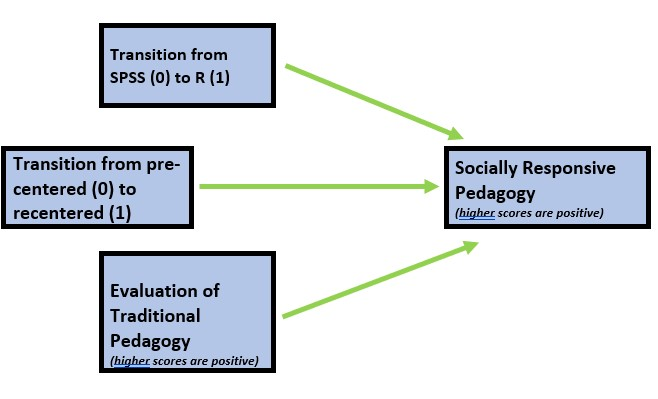
\includegraphics{Worked_Examples/images/homeworked_model.jpg}
\caption{An image of our the prediction model for the homeworked example.}
\end{figure}

\hypertarget{import-data-1}{%
\subsubsection*{Import data}\label{import-data-1}}


\begin{Shaded}
\begin{Highlighting}[]
\NormalTok{raw }\OtherTok{\textless{}{-}} \FunctionTok{readRDS}\NormalTok{(}\StringTok{"ReC.rds"}\NormalTok{)}
\FunctionTok{nrow}\NormalTok{(raw)}
\end{Highlighting}
\end{Shaded}

\begin{verbatim}
[1] 310
\end{verbatim}

\hypertarget{apply-inclusionaryexclusionary-criteria}{%
\subsubsection*{Apply inclusionary/exclusionary criteria}\label{apply-inclusionaryexclusionary-criteria}}


Because this data is publicly posted on the Open Science Framework, it was necessary for me to already exclude those individuals. This data was unique in that students could freely write some version of ``Opt out.'' My original code included a handful of versions, but here was the basic form:

\begin{Shaded}
\begin{Highlighting}[]
\CommentTok{\# testing to see if my code worked raw \textless{}{-} dplyr::filter (raw,}
\CommentTok{\# SPFC.Decolonize.Opt.Out != \textquotesingle{}Okay\textquotesingle{})}
\NormalTok{raw }\OtherTok{\textless{}{-}}\NormalTok{ dplyr}\SpecialCharTok{::}\FunctionTok{filter}\NormalTok{(raw, SPFC.Decolonize.Opt.Out }\SpecialCharTok{!=} \StringTok{"Opt Out"}\NormalTok{)}
\end{Highlighting}
\end{Shaded}

I want to exclude students' responses for the ANOVA and psychometrics courses.

\begin{Shaded}
\begin{Highlighting}[]
\NormalTok{raw }\OtherTok{\textless{}{-}}\NormalTok{ dplyr}\SpecialCharTok{::}\FunctionTok{filter}\NormalTok{(raw, Course }\SpecialCharTok{==} \StringTok{"Multivariate"}\NormalTok{)}
\end{Highlighting}
\end{Shaded}

At this point, these my only inclusion/exclusion criteria. I can determine how many students (who consented) completed any portion of the survey.

\begin{Shaded}
\begin{Highlighting}[]
\FunctionTok{nrow}\NormalTok{(raw)}
\end{Highlighting}
\end{Shaded}

\begin{verbatim}
[1] 84
\end{verbatim}

\hypertarget{format-any-variables-that-shouldnt-be-imputed-in-their-raw-form}{%
\subsubsection{Format any variables that shouldn't be imputed in their raw form}\label{format-any-variables-that-shouldnt-be-imputed-in-their-raw-form}}

Let's first create a df with the item-level variables that will fuel our model.

In addition to the variables in our model, we will include four auxiliary variables. These include Dept (Department: Clinical or Industrial-Organizational) and four additional course evaluation items: OvInstructor, MyContribution, IncrInterest, IncrUnderstanding.

Let's check the structure to be certain that \emph{StatsPkg} (SPSS, R) and \emph{Centered} (Pre, Re) are ordered factors. We also want the course evaluation items to be integer (or numerical).

\begin{Shaded}
\begin{Highlighting}[]
\NormalTok{mimp\_df }\OtherTok{\textless{}{-}}\NormalTok{ dplyr}\SpecialCharTok{::}\FunctionTok{select}\NormalTok{(raw, deID, StatsPkg, Centering, ClearResponsibilities,}
\NormalTok{    EffectiveAnswers, Feedback, ClearOrganization, ClearPresentation, InclusvClassrm,}
\NormalTok{    EquitableEval, MultPerspectives, DEIintegration, Dept, OvInstructor,}
\NormalTok{    MyContribution, IncrInterest, IncrUnderstanding)}
\FunctionTok{str}\NormalTok{(mimp\_df)}
\end{Highlighting}
\end{Shaded}

\begin{verbatim}
Classes 'data.table' and 'data.frame':  84 obs. of  17 variables:
 $ deID                 : int  11 12 13 14 15 16 17 18 35 19 ...
 $ StatsPkg             : Factor w/ 2 levels "SPSS","R": 2 2 2 2 2 2 2 2 2 2 ...
 $ Centering            : Factor w/ 2 levels "Pre","Re": 2 2 2 2 2 2 2 2 2 2 ...
 $ ClearResponsibilities: int  4 5 5 5 4 3 5 5 3 5 ...
 $ EffectiveAnswers     : int  4 5 5 4 4 3 5 5 4 4 ...
 $ Feedback             : int  4 5 4 4 5 4 5 4 4 5 ...
 $ ClearOrganization    : int  3 5 5 4 4 3 5 5 4 5 ...
 $ ClearPresentation    : int  4 5 5 3 4 2 5 4 5 5 ...
 $ InclusvClassrm       : int  5 5 5 5 5 4 5 5 5 5 ...
 $ EquitableEval        : int  4 5 5 5 4 4 5 4 5 5 ...
 $ MultPerspectives     : int  4 5 5 5 5 5 5 4 5 5 ...
 $ DEIintegration       : int  5 5 5 5 5 5 5 5 5 5 ...
 $ Dept                 : chr  "CPY" "CPY" "CPY" "CPY" ...
 $ OvInstructor         : int  3 5 5 3 5 2 5 4 5 5 ...
 $ MyContribution       : int  4 5 4 3 4 3 5 4 4 5 ...
 $ IncrInterest         : int  4 5 4 3 4 3 5 4 5 4 ...
 $ IncrUnderstanding    : int  4 5 5 3 4 3 5 4 5 5 ...
 - attr(*, ".internal.selfref")=<externalptr> 
\end{verbatim}

\begin{Shaded}
\begin{Highlighting}[]
\NormalTok{mimp\_df}\SpecialCharTok{$}\NormalTok{Dept }\OtherTok{\textless{}{-}} \FunctionTok{factor}\NormalTok{(mimp\_df}\SpecialCharTok{$}\NormalTok{Dept, }\AttributeTok{levels =} \FunctionTok{c}\NormalTok{(}\StringTok{"CPY"}\NormalTok{, }\StringTok{"ORG"}\NormalTok{))}
\FunctionTok{str}\NormalTok{(mimp\_df}\SpecialCharTok{$}\NormalTok{Dept)}
\end{Highlighting}
\end{Shaded}

\begin{verbatim}
 Factor w/ 2 levels "CPY","ORG": 1 1 1 1 1 1 1 1 1 1 ...
\end{verbatim}

We should eliminate case with greater than 50\% missingness.

\begin{Shaded}
\begin{Highlighting}[]
\FunctionTok{library}\NormalTok{(tidyverse)}
\CommentTok{\#Calculating number and proportion of item{-}level missingness}
\NormalTok{mimp\_df}\SpecialCharTok{$}\NormalTok{nmiss }\OtherTok{\textless{}{-}}\NormalTok{ mimp\_df}\SpecialCharTok{\%\textgreater{}\%}
\NormalTok{    dplyr}\SpecialCharTok{::}\FunctionTok{select}\NormalTok{(StatsPkg}\SpecialCharTok{:}\NormalTok{IncrUnderstanding) }\SpecialCharTok{\%\textgreater{}\%} \CommentTok{\#the colon allows us to include all variables between the two listed (the variables need to be in order)}
\NormalTok{    is.na }\SpecialCharTok{\%\textgreater{}\%} 
\NormalTok{    rowSums}

\NormalTok{mimp\_df}\OtherTok{\textless{}{-}}\NormalTok{ mimp\_df}\SpecialCharTok{\%\textgreater{}\%}
\NormalTok{  dplyr}\SpecialCharTok{::}\FunctionTok{mutate}\NormalTok{(}\AttributeTok{prop\_miss =}\NormalTok{ (nmiss}\SpecialCharTok{/}\DecValTok{13}\NormalTok{)}\SpecialCharTok{*}\DecValTok{100}\NormalTok{) }\CommentTok{\#11 is the number of variables included in calculating the proportion}

\NormalTok{mimp\_df }\OtherTok{\textless{}{-}} \FunctionTok{filter}\NormalTok{(mimp\_df, prop\_miss }\SpecialCharTok{\textless{}=} \DecValTok{50}\NormalTok{)  }\CommentTok{\#update df to have only those with at least 50\% of complete data}
\end{Highlighting}
\end{Shaded}

Once again, trim the df to include only the data to be included in the imputation

\begin{Shaded}
\begin{Highlighting}[]
\NormalTok{mimp\_df }\OtherTok{\textless{}{-}}\NormalTok{  dplyr}\SpecialCharTok{::}\FunctionTok{select}\NormalTok{(mimp\_df, deID, StatsPkg, Centering,ClearResponsibilities, EffectiveAnswers, Feedback, ClearOrganization, ClearPresentation, InclusvClassrm, EquitableEval, MultPerspectives, DEIintegration, Dept, OvInstructor, MyContribution, IncrInterest, IncrUnderstanding)}
\end{Highlighting}
\end{Shaded}

\hypertarget{multiply-impute-a-minimum-of-5-sets-of-data}{%
\subsubsection{Multiply impute a minimum of 5 sets of data}\label{multiply-impute-a-minimum-of-5-sets-of-data}}

Because multiple imputation is a \emph{random} process, if we all want the same answers we need to set a \emph{random seed.}

\begin{Shaded}
\begin{Highlighting}[]
\FunctionTok{set.seed}\NormalTok{(}\DecValTok{2309034}\NormalTok{)  }\CommentTok{\#you can pick any number you want, today I\textquotesingle{}m using today\textquotesingle{}s datestamp}
\end{Highlighting}
\end{Shaded}

The program we will use is \emph{mice}. \emph{mice} assumes that each variable has a distribution and it imputes missing variables according to that distribution.

This means we need to correctly specify each variable's format/role. \emph{mice} will automatically choose a distribution (think ``format'') for each variable; we can override this by changing the methods' characteristics.

The following code sets up the structure for the imputation. This follows the Katitas example.

\begin{Shaded}
\begin{Highlighting}[]
\FunctionTok{library}\NormalTok{(mice)}
\CommentTok{\# runs the mice code with 0 iterations}
\NormalTok{imp }\OtherTok{\textless{}{-}} \FunctionTok{mice}\NormalTok{(mimp\_df, }\AttributeTok{maxit =} \DecValTok{0}\NormalTok{)}
\CommentTok{\# Extract predictor Matrix and methods of imputation}
\NormalTok{predM }\OtherTok{=}\NormalTok{ imp}\SpecialCharTok{$}\NormalTok{predictorMatrix}
\NormalTok{meth }\OtherTok{=}\NormalTok{ imp}\SpecialCharTok{$}\NormalTok{method}
\NormalTok{log }\OtherTok{=}\NormalTok{ imp}\SpecialCharTok{$}\NormalTok{log}
\end{Highlighting}
\end{Shaded}

Here we code what format/role each variable should be.

\begin{Shaded}
\begin{Highlighting}[]
\CommentTok{\# These variables are left in the dataset, but setting them = 0 means}
\CommentTok{\# they are not used as predictors.  We want our ID to be retained in}
\CommentTok{\# the df.  There\textquotesingle{}s nothing missing from it, and we don\textquotesingle{}t want it used}
\CommentTok{\# as a predictor, so it will just hang out.}
\NormalTok{predM[, }\FunctionTok{c}\NormalTok{(}\StringTok{"deID"}\NormalTok{)] }\OtherTok{=} \DecValTok{0}

\CommentTok{\# If you like, view the first few rows of the predictor matrix}
\CommentTok{\# head(predM)}

\CommentTok{\# We don\textquotesingle{}t have any ordered categorical variables, but if we did we}
\CommentTok{\# would follow this format poly \textless{}{-} c(\textquotesingle{}Var1\textquotesingle{}, \textquotesingle{}Var2\textquotesingle{})}

\CommentTok{\# We have three dichotomous variables}
\NormalTok{log }\OtherTok{\textless{}{-}} \FunctionTok{c}\NormalTok{(}\StringTok{"StatsPkg"}\NormalTok{, }\StringTok{"Centering"}\NormalTok{, }\StringTok{"Dept"}\NormalTok{)}

\CommentTok{\# Unordered categorical variables (nominal variables), but if we did}
\CommentTok{\# we would follow this format poly2 \textless{}{-} c(\textquotesingle{}format\textquotesingle{})}

\CommentTok{\# Turn their methods matrix into the specified imputation models}
\CommentTok{\# Remove the hashtag if you have any of these variables meth[poly] =}
\CommentTok{\# \textquotesingle{}polr\textquotesingle{}}
\NormalTok{meth[log] }\OtherTok{=} \StringTok{"logreg"}
\CommentTok{\# meth[poly2] = \textquotesingle{}polyreg\textquotesingle{}}

\NormalTok{meth}
\end{Highlighting}
\end{Shaded}

\begin{verbatim}
                 deID              StatsPkg             Centering 
                   ""              "logreg"              "logreg" 
ClearResponsibilities      EffectiveAnswers              Feedback 
                "pmm"                    ""                 "pmm" 
    ClearOrganization     ClearPresentation        InclusvClassrm 
                   ""                    ""                 "pmm" 
        EquitableEval      MultPerspectives        DEIintegration 
                   ""                 "pmm"                 "pmm" 
                 Dept          OvInstructor        MyContribution 
             "logreg"                    ""                    "" 
         IncrInterest     IncrUnderstanding 
                "pmm"                    "" 
\end{verbatim}

This list (meth) contains all our variables; ``pmm'' is the default and is the ``predictive mean matching'' process used. We see that \emph{StatsPkg} and \emph{Centering} are noted as ``logreg.'' This is because they are dichotomous variables. If there is \emph{``\,``} underneath it means the data is complete. The data will be used in imputing other data, but none of that data will be imputed.

Our variables of interest are now configured to be imputed with the imputation method we specified. Empty cells in the method matrix mean that those variables aren't going to be imputed.

If a variable has no missing values, it is automatically set to be empty. We can also manually set variables to not be imputed with the \emph{meth{[}variable{]}=``\,``} command.

The code below begins the imputation process. We are asking for 5 datasets. If you have many cases and many variables, this can take awhile. How many imputations? Recommendations have ranged as low as five to several hundred.

\begin{Shaded}
\begin{Highlighting}[]
\CommentTok{\# With this command, we tell mice to impute the anesimpor2 data,}
\CommentTok{\# create 5vvdatasets, use predM as the predictor matrix and don\textquotesingle{}t}
\CommentTok{\# print the imputation process.  If you would like to see the process}
\CommentTok{\# (or if the process is failing to execute) set print as TRUE; seeing}
\CommentTok{\# where the execution halts can point to problematic variables (more}
\CommentTok{\# notes at end of lecture)}

\NormalTok{imp2 }\OtherTok{\textless{}{-}} \FunctionTok{mice}\NormalTok{(mimp\_df, }\AttributeTok{maxit =} \DecValTok{5}\NormalTok{, }\AttributeTok{predictorMatrix =}\NormalTok{ predM, }\AttributeTok{method =}\NormalTok{ meth,}
    \AttributeTok{log =}\NormalTok{ log, }\AttributeTok{print =} \ConstantTok{FALSE}\NormalTok{)}
\end{Highlighting}
\end{Shaded}

We need to create a ``long file'' that stacks all the imputed data. Looking at the df in R Studio shows us that when imp = 0 (the pe-imputed data), there is still missingness. As we scroll through the remaining imputations, there are no NA cells.

\begin{Shaded}
\begin{Highlighting}[]
\CommentTok{\# First, turn the datasets into long format This procedure is, best I}
\CommentTok{\# can tell, unique to mice and wouldn\textquotesingle{}t work for repeated measures}
\CommentTok{\# designs}
\NormalTok{mimp\_long }\OtherTok{\textless{}{-}}\NormalTok{ mice}\SpecialCharTok{::}\FunctionTok{complete}\NormalTok{(imp2, }\AttributeTok{action =} \StringTok{"long"}\NormalTok{, }\AttributeTok{include =} \ConstantTok{TRUE}\NormalTok{)}
\end{Highlighting}
\end{Shaded}

If we look at it, we can see 6 sets of data. If the \emph{deID} variable is sorted we see that:

\begin{itemize}
\tightlist
\item
  .imp = 0 is the unimputed set; there are still missing values
\item
  .imp = 1, 2, 3, or 5 has no missing values for the variables we included in the imputation
\end{itemize}

With the code below we can see the proportion of missingness for each variable (that has missing data), sorted from highest to lowest.

\begin{Shaded}
\begin{Highlighting}[]
\NormalTok{p\_missing\_mimp\_long }\OtherTok{\textless{}{-}} \FunctionTok{unlist}\NormalTok{(}\FunctionTok{lapply}\NormalTok{(mimp\_long, }\ControlFlowTok{function}\NormalTok{(x) }\FunctionTok{sum}\NormalTok{(}\FunctionTok{is.na}\NormalTok{(x))))}\SpecialCharTok{/}\FunctionTok{nrow}\NormalTok{(mimp\_long)}
\FunctionTok{sort}\NormalTok{(p\_missing\_mimp\_long[p\_missing\_mimp\_long }\SpecialCharTok{\textgreater{}} \DecValTok{0}\NormalTok{], }\AttributeTok{decreasing =} \ConstantTok{TRUE}\NormalTok{)  }\CommentTok{\#check to see if this works}
\end{Highlighting}
\end{Shaded}

\begin{verbatim}
       DEIintegration        InclusvClassrm              Feedback 
          0.027777778           0.007936508           0.003968254 
ClearResponsibilities      MultPerspectives          IncrInterest 
          0.001984127           0.001984127           0.001984127 
\end{verbatim}

Because our imputation was item-level, we need to score the variables with scales/subscales.

Traditional pedagogy is a predictor variable that needs to be created by calculating the mean if at least 75\% of the items are non-missing. None of the items need to be reverse-scored. I will return to working with the \emph{scrub\_df} data.

\begin{Shaded}
\begin{Highlighting}[]
\CommentTok{\# this seems to work when I build the book, but not in \textquotesingle{}working the}
\CommentTok{\# problem\textquotesingle{}}
\NormalTok{TradPed\_vars }\OtherTok{\textless{}{-}} \FunctionTok{c}\NormalTok{(}\StringTok{"ClearResponsibilities"}\NormalTok{, }\StringTok{"EffectiveAnswers"}\NormalTok{, }\StringTok{"Feedback"}\NormalTok{,}
    \StringTok{"ClearOrganization"}\NormalTok{, }\StringTok{"ClearPresentation"}\NormalTok{)}
\CommentTok{\# mimp\_long$TradPed \textless{}{-} sjstats::mean\_n(mimp\_long[, TradPed\_vars],}
\CommentTok{\# .75)}

\CommentTok{\# this seems to work when I \textquotesingle{}work the problem\textquotesingle{} (but not when I build}
\CommentTok{\# the book) the difference is the two dots before the last SRPed\_vars}
\NormalTok{mimp\_long}\SpecialCharTok{$}\NormalTok{TradPed }\OtherTok{\textless{}{-}}\NormalTok{ sjstats}\SpecialCharTok{::}\FunctionTok{mean\_n}\NormalTok{(mimp\_long[, TradPed\_vars], }\FloatTok{0.75}\NormalTok{)}
\end{Highlighting}
\end{Shaded}

The dependent variable is socially responsive pedagogy. It needs to be created by calculating the mean if at least 75\% of the items are non-missing. None of the items need to be reverse-scored.

\begin{Shaded}
\begin{Highlighting}[]
\CommentTok{\# this seems to work when I build the book, but not in \textquotesingle{}working the}
\CommentTok{\# problem\textquotesingle{} SRPed\_vars \textless{}{-} c(\textquotesingle{}InclusvClassrm\textquotesingle{},\textquotesingle{}EquitableEval\textquotesingle{},}
\CommentTok{\# \textquotesingle{}MultPerspectives\textquotesingle{}, \textquotesingle{}DEIintegration\textquotesingle{}) mimp\_long$SRPed \textless{}{-}}
\CommentTok{\# sjstats::mean\_n(mimp\_long[, SRPed\_vars], .75)}

\CommentTok{\# this seems to work when I \textquotesingle{}work the problem\textquotesingle{} (but not when I build}
\CommentTok{\# the book) the difference is the two dots before the last SRPed\_vars}
\NormalTok{SRPed\_vars }\OtherTok{\textless{}{-}} \FunctionTok{c}\NormalTok{(}\StringTok{"InclusvClassrm"}\NormalTok{, }\StringTok{"EquitableEval"}\NormalTok{, }\StringTok{"MultPerspectives"}\NormalTok{,}
    \StringTok{"DEIintegration"}\NormalTok{)}
\NormalTok{mimp\_long}\SpecialCharTok{$}\NormalTok{SRPed }\OtherTok{\textless{}{-}}\NormalTok{ sjstats}\SpecialCharTok{::}\FunctionTok{mean\_n}\NormalTok{(mimp\_long[, SRPed\_vars], }\FloatTok{0.75}\NormalTok{)}
\end{Highlighting}
\end{Shaded}

\hypertarget{run-a-regression-for-multiply-imputed-data-with-at-least-three-variables}{%
\subsubsection{Run a regression (for multiply imputed data) with at least three variables}\label{run-a-regression-for-multiply-imputed-data-with-at-least-three-variables}}

For comparison, here was the script when we used the AIA approach for managing missingness:

\begin{quote}
\begin{quote}
SRPed\_fit \textless- lm(SRPed \textasciitilde{} StatsPkg + Centering + TradPed, data = scored)
\end{quote}
\end{quote}

In order for the regression to use multiply imputed data, it must be a ``mids'' (multiply imputed data sets) type

\begin{Shaded}
\begin{Highlighting}[]
\CommentTok{\# Convert to mids type {-} mice can work with this type}
\NormalTok{mimp\_mids }\OtherTok{\textless{}{-}} \FunctionTok{as.mids}\NormalTok{(mimp\_long)}
\end{Highlighting}
\end{Shaded}

Here's what we do with imputed data:

\begin{Shaded}
\begin{Highlighting}[]
\NormalTok{fitimp }\OtherTok{\textless{}{-}} \FunctionTok{with}\NormalTok{(mimp\_mids, }\FunctionTok{lm}\NormalTok{(SRPed }\SpecialCharTok{\textasciitilde{}}\NormalTok{ StatsPkg }\SpecialCharTok{+}\NormalTok{ Centering }\SpecialCharTok{+}\NormalTok{ TradPed))}
\end{Highlighting}
\end{Shaded}

In this process, 5 individual, OLS, regressions are being conducted and the results being pooled into this single set.

\begin{Shaded}
\begin{Highlighting}[]
\CommentTok{\# to get the 5, individual imputations}
\FunctionTok{summary}\NormalTok{(fitimp)}
\end{Highlighting}
\end{Shaded}

\begin{verbatim}
# A tibble: 20 x 6
   term        estimate std.error statistic  p.value  nobs
   <chr>          <dbl>     <dbl>     <dbl>    <dbl> <int>
 1 (Intercept)    1.90     0.310      6.13  3.13e- 8    84
 2 StatsPkgR      0.187    0.118      1.59  1.16e- 1    84
 3 CenteringRe    0.117    0.108      1.09  2.79e- 1    84
 4 TradPed        0.565    0.0659     8.56  6.30e-13    84
 5 (Intercept)    1.94     0.314      6.17  2.62e- 8    84
 6 StatsPkgR      0.191    0.119      1.60  1.13e- 1    84
 7 CenteringRe    0.110    0.109      1.01  3.17e- 1    84
 8 TradPed        0.557    0.0667     8.36  1.63e-12    84
 9 (Intercept)    1.96     0.313      6.26  1.80e- 8    84
10 StatsPkgR      0.178    0.119      1.50  1.38e- 1    84
11 CenteringRe    0.111    0.109      1.02  3.10e- 1    84
12 TradPed        0.555    0.0665     8.35  1.69e-12    84
13 (Intercept)    2.03     0.325      6.24  1.98e- 8    84
14 StatsPkgR      0.185    0.123      1.50  1.38e- 1    84
15 CenteringRe    0.104    0.113      0.918 3.62e- 1    84
16 TradPed        0.539    0.0691     7.80  1.95e-11    84
17 (Intercept)    1.91     0.306      6.26  1.77e- 8    84
18 StatsPkgR      0.158    0.116      1.36  1.78e- 1    84
19 CenteringRe    0.117    0.107      1.10  2.76e- 1    84
20 TradPed        0.567    0.0649     8.73  2.93e-13    84
\end{verbatim}

\begin{Shaded}
\begin{Highlighting}[]
\FunctionTok{summary}\NormalTok{(}\FunctionTok{pool}\NormalTok{(fitimp))}
\end{Highlighting}
\end{Shaded}

\begin{verbatim}
         term  estimate  std.error statistic       df              p.value
1 (Intercept) 1.9480744 0.31833535  6.119567 74.55114 0.000000040039269753
2   StatsPkgR 0.1798400 0.11996611  1.499090 76.64577 0.137957984459613908
3 CenteringRe 0.1117906 0.10918108  1.023901 77.81162 0.309054914517060075
4     TradPed 0.5564494 0.06768356  8.221338 74.26455 0.000000000004825124
\end{verbatim}

\begin{quote}
\begin{quote}
Results of a multiple regression predicting the socially responsive course evaluation ratings indicated that neither the transition from SPSS to R (\(B = 0.178, p = 0.135\)) nor the transition to an explicitly recentered curriculum (\(B = 0.116, p = 0.285) led to statistically significant diferences. In contrast, traditional pedagogy had a strong, positive effect on evaluations of socially responsive pedagogy (\)B = 0.571, p \textless{} 0.001). Results of the regression model are presented in Table 2.
\end{quote}
\end{quote}

\hypertarget{apa-style-write-up-of-the-multiple-imputation-section-of-data-diagnostics}{%
\subsubsection{APA style write-up of the multiple imputation section of data diagnostics}\label{apa-style-write-up-of-the-multiple-imputation-section-of-data-diagnostics}}

My write-up draws from some of the results we obtained in the homeworked example at the end of the \protect\hyperlink{DataDx}{Data Dx} chapter.

\begin{quote}
\begin{quote}
This is a secondary analysis of data involved in a more comprehensive dataset that included students taking multiple statistics courses (\emph{N} = 310). Having retrieved this data from a repository in the Open Science Framework, only those who consented to participation in the study were included. Data used in these analyses were 84 students who completed the multivariate clas.
\end{quote}
\end{quote}

\begin{quote}
\begin{quote}
Across cases that were deemed eligible on the basis of the inclusion/exclusion criteria, missingness ranged from 0 to 100\%. Across the dataset, 3.86\% of cells had missing data and 87.88\% of cases had nonmissing data. At this stage in the analysis, missingness for all cases did not exceed 50\% \citep{katitas_getting_2019} and they were all included in the multiple imputation .
\end{quote}
\end{quote}

\begin{quote}
\begin{quote}
Regarding the distributional characteristics of the data, skew and kurtosis values of the variables fell below the values of 3 (skew) and 10 (kurtosis) that Kline suggests are concerning \citeyearpar{kline_principles_2016}. Results of the Shapiro-Wilk test of normality indicate that our variables assessing the traditional pedagogy (\(W = 0.830, p < 0.001\)) and socially responsive pedagogy (0.818, p \textless{} 0.001) are statistically significantly different than a normal distribution. Inspection of distributions of the variables indicated that both course evaluation variables were negatively skewed, with a large proportion of high scores.
\end{quote}
\end{quote}

\begin{quote}
\begin{quote}
We evaluated multivariate normality with the Mahalanobis distance test. Specifically, we used the \emph{psych::outlier()} function and included both continuous variables in the calculation. Our visual inspection of the Q-Q plot suggested that the plotted line strayed from the straight line as the quantiles increased. Additionally, we appended the Mahalanobis distance scores as a variable to the data. Analyzing this variable, we found that 2 cases exceed three standard deviations beyond the median.
\end{quote}
\end{quote}

\begin{quote}
\begin{quote}
We managed missing data with multiple imputation \citep{enders_multiple_2017, katitas_getting_2019}. We imputed five sets of data with the R package, \emph{mice} (v. 3.13) -- a program that utilizes conditional multiple imputation. The imputation included the 9 item-level variables that comprised our scales and the dichotomous variable representing traditional pedagogy and socially responsive pedagogy. We also included five auxiliary variables (four variables from the course evaluation and the whether the student was from the Clinical or Industrial-Organizational Psychology program).
\end{quote}
\end{quote}

\hypertarget{apa-style-write-up-regression-results}{%
\subsubsection{APA style write-up regression results}\label{apa-style-write-up-regression-results}}

\begin{quote}
\begin{quote}
Results of a multiple regression predicting the socially responsive course evaluation ratings indicated that neither the transition from SPSS to R (\(B = 0.178, p = 0.135\)) nor the transition to an explicitly recentered curriculum (\(B = 0.116, p = 0.285) led to statistically significant diferences. In contrast, traditional pedagogy had a strong, positive effect on evaluations of socially responsive pedagogy (\)B = 0.571, p \textless{} 0.001). Results of the regression model are presented in Table 2.
\end{quote}
\end{quote}

\emph{As in the lesson itself, I used the data diagnostics that we did in the AIA method. It feels to me like these should be calculated with the multiply imputed data (i.e., 5 sets, with pooled estimates and standard errors), but I do not see that modeled -- anywhere in tutorials I consulted.}

\hypertarget{MED}{%
\chapter*{MEDIATION}\label{MED}}


\hypertarget{SimpleMed}{%
\chapter{Simple Mediation}\label{SimpleMed}}

\href{https://youtube.com/playlist?list=PLtz5cFLQl4KO-j2YBYGwyUl34pIXzNVST\&si=Jp5LJf35y5T-VbFb}{Screencasted Lecture Link}

The focus of this lecture is to estimate indirect effects (aka ``mediation''). We examine the logic/design required to support the argument that \emph{mediation} is the \emph{mechanism} that explains the X --\textgreater{} Y relationship. We also work three examples (one with covariates).

At the outset, please note that although I rely heavily on Hayes \citeyearpar{hayes_introduction_2018} text and materials, I am using the R package \emph{lavaan} in these chapters. In recent years, Hayes has introduced a \href{https://www.processmacro.org/index.html}{PROCESS macro for R}. Because I am not yet up-to-speed on using this macro (it is not a typical R package) and because ReCentering Psych Stats uses \emph{lavaan} for confirmatory factor analysis and structural equation modeling, I have chosen to utilize the \emph{lavaan} package. A substantial difference is that the PROCESS macros use ordinary least squares and \emph{lavaan} uses maximum likelihood estimators.

\hypertarget{navigating-this-lesson-4}{%
\section{Navigating this Lesson}\label{navigating-this-lesson-4}}

There is about 1 hour and 10 minutes of lecture. If you work through the materials with me it would be plan for an additional 1.5 hours.

While the majority of R objects and data you will need are created within the R script that sources the chapter, ocasionally there are some that cannot be created from within the R framework. Additionally, sometimes links fail. All original materials are provided at the \href{https://github.com/lhbikos/ReC_MultivModel}{Github site} that hosts the book. More detailed guidelines for ways to access all these materials are provided in the OER's \protect\hyperlink{ReCintro}{introduction}

\hypertarget{learning-objectives-4}{%
\subsection{Learning Objectives}\label{learning-objectives-4}}

Learning objectives from this lecture include the following:

\begin{itemize}
\tightlist
\item
  Define mediation and indirect effect.
\item
  Distinguish the role of a mediating variable from independent variables, covariates, and moderators.
\item
  Identify the conditions upon which there can be justification to support the presence of a mediated effect.
\item
  Articulate the arguments for and against using the term, ``mediation.''
\item
  Using the R package \emph{lavaan},

  \begin{itemize}
  \tightlist
  \item
    specify a model with indirect effects,
  \item
    identify and interpret B weights, \emph{p} values, and \emph{CIs} for total, direct, and indirect effects,
  \item
    calculate the total effects of X and M on Y,
  \item
    identify the proportion of variance accounted for in predicting M and Y.
  \end{itemize}
\item
  Hand calculate the values of an indirect, direct, and total effects from statistical output or a figure (just the \(B\) or \(\beta\), not the significance level)
\end{itemize}

\hypertarget{planning-for-practice-4}{%
\subsection{Planning for Practice}\label{planning-for-practice-4}}

The following suggestions for practice will involve specifying, testing, and interpreting a model with a single indirect effect (mediator).

\begin{itemize}
\tightlist
\item
  Rework the problem in the chapter by changing the random seed in the code that simulates the data. This should provide minor changes to the data, but the results will likely be very similar.
\item
  There are a number of variables in the dataset and there were a handful of simple mediations conducted in the journal article that sources the research vignette. Swap out one or more variables in the model of simple mediation and compare your solution to the one in the chapter and/or the research article.
\item
  Conduct a simple mediation with data to which you have access. This could include data you simulate on your own or from a published article.
\end{itemize}

\hypertarget{readings-resources-4}{%
\subsection{Readings \& Resources}\label{readings-resources-4}}

In preparing this chapter, I drew heavily from the following resource(s). Other resources are cited (when possible, linked) in the text with complete citations in the reference list.

\begin{itemize}
\tightlist
\item
  Hayes, A. F. (2022). \emph{Introduction to mediation, moderation, and conditional process analysis: A regression-based approach}. New York, NY: Guilford Press.

  \begin{itemize}
  \tightlist
  \item
    \textbf{Chapter 3, The simple mediation model}: Hayes' text is another great example of a teaching tool that is accessible at both procedural and conceptual levels. I especially appreciate his attention to the controversies (even those directed toward his work). We deviate from his text in that we are not using the PROCESS macro\ldots and I'll address those concerns in the lecture.
  \item
    \textbf{Chapter 4, Causal steps, scaling, confounding, and causal order}: A great chapter that addresses ``What happened to Baron \& Kenny''; partial v complete mediation; and conditions required for claims of causality. Procedurally, our focus in this chapter is on the role of covariates.
  \item
    \textbf{Appendix A: Using PROCESS}: An essential tool for PROCESS users because, even when we are in the R environment, this is the ``idea book.'' That is, the place where all the path models are presented in figures.
  \end{itemize}
\item
  Kim, P. Y., Kendall, D. L., \& Cheon, H.-S. (2017). Racial microaggressions, cultural mistrust, and mental health outcomes among Asian American college students. \emph{American Journal of Orthopsychiatry, 87}(6), 663--670. \url{https://doi-org.ezproxy.spu.edu/10.1037/ort0000203}
\end{itemize}

\hypertarget{packages-4}{%
\subsection{Packages}\label{packages-4}}

The script below will (a) check to see if the following packages are installed on your computer and, if not (b) install them.

\begin{Shaded}
\begin{Highlighting}[]
\CommentTok{\# will install the package if not already installed}
\ControlFlowTok{if}\NormalTok{ (}\SpecialCharTok{!}\FunctionTok{require}\NormalTok{(lavaan)) \{}
    \FunctionTok{install.packages}\NormalTok{(}\StringTok{"lavaan"}\NormalTok{)}
\NormalTok{\}}
\ControlFlowTok{if}\NormalTok{ (}\SpecialCharTok{!}\FunctionTok{require}\NormalTok{(semPlot)) \{}
    \FunctionTok{install.packages}\NormalTok{(}\StringTok{"semPlot"}\NormalTok{)}
\NormalTok{\}}
\ControlFlowTok{if}\NormalTok{ (}\SpecialCharTok{!}\FunctionTok{require}\NormalTok{(tidyverse)) \{}
    \FunctionTok{install.packages}\NormalTok{(}\StringTok{"tidyverse"}\NormalTok{)}
\NormalTok{\}}
\ControlFlowTok{if}\NormalTok{ (}\SpecialCharTok{!}\FunctionTok{require}\NormalTok{(psych)) \{}
    \FunctionTok{install.packages}\NormalTok{(}\StringTok{"psych"}\NormalTok{)}
\NormalTok{\}}
\ControlFlowTok{if}\NormalTok{ (}\SpecialCharTok{!}\FunctionTok{require}\NormalTok{(formattable)) \{}
    \FunctionTok{install.packages}\NormalTok{(}\StringTok{"formattable"}\NormalTok{)}
\NormalTok{\}}
\ControlFlowTok{if}\NormalTok{ (}\SpecialCharTok{!}\FunctionTok{require}\NormalTok{(semTable)) \{}
    \FunctionTok{install.packages}\NormalTok{(}\StringTok{"semTable"}\NormalTok{)}
\NormalTok{\}}
\end{Highlighting}
\end{Shaded}

\hypertarget{estimating-indirect-effects-the-analytic-approach-often-termed-mediation}{%
\section{\texorpdfstring{Estimating Indirect Effects (the analytic approach often termed \emph{mediation})}{Estimating Indirect Effects (the analytic approach often termed mediation)}}\label{estimating-indirect-effects-the-analytic-approach-often-termed-mediation}}

\hypertarget{the-definitional-and-conceptual}{%
\subsection{The definitional and conceptual}\label{the-definitional-and-conceptual}}

As in Hayes text \citeyearpar{hayes_introduction_2018}, we will differentiate between \emph{moderation} and \emph{mediation}. \emph{Conditional process analysis} involves both! With each of these, we are seeking to understand the \emph{mechanism} at work that leads to the relationship (be it correlational, predictive, or causal)

Even though this process has sometimes been termed \emph{causal modeling}, Hayes argues that his \emph{statistical approach} is not claiming to determine \emph{cause}; that is really left to the argument of the research design.

\textbf{Moderation} (a review):

\begin{itemize}
\tightlist
\item
  Answers questions of \emph{when} or \emph{for whom} and is often the source of the answer, \emph{it depends}.
\item
  Think of our \emph{interaction} effects in ANOVA and regression
\item
  The effect of X on some variable Y is moderated by W if its size, sign, or strength depends on, or can be predicted, by W. Then we can say, ``W is a \emph{moderator} of X's effect on Y'' or ``W and X \emph{interact} in their influence on Y.''
\item
  The image below illustrates moderation with \emph{conceptual} and \emph{statistical} diagrams. Note that three predictors (IV, DV, their interaction) point to the DV.
\end{itemize}

\begin{figure}
\centering
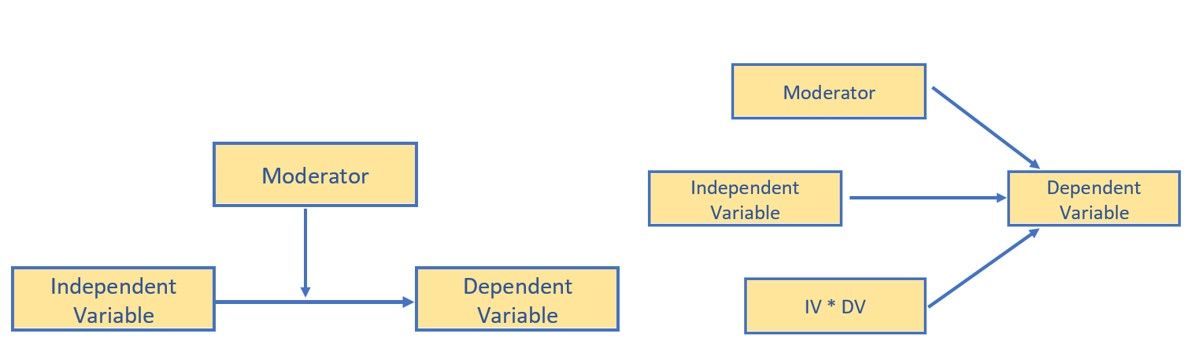
\includegraphics{images/SimpleMed/ModConcStat.jpg}
\caption{Image of Hayes'style conceptual and statistical diagrams of a simple moderation}
\end{figure}

The classic plot of moderation results is often the best way to detect that an interaction was included in the analysis and helps understand the \emph{conditional} (e.g., for whom, under what conditions) nature of the analysis.

\begin{figure}
\centering
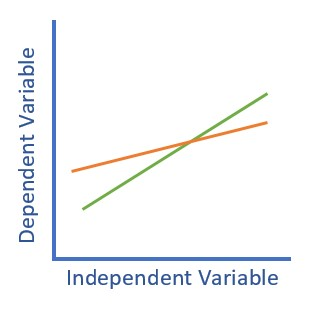
\includegraphics{images/SimpleMed/SimpleInteraction.jpg}
\caption{Image of classic interaction graph that illustrates a moderated effect. The IV is on the X axis, DV on the Y axis, and two intersecting lines represent the differential/moderated effect of the IV on the DV by the moderator}
\end{figure}

\textbf{Mediation}:

\begin{itemize}
\tightlist
\item
  Answers questions of \emph{how} (I also think \emph{through} and \emph{via} to describe the proposed mediating mechanism)
\item
  Paths in a mediation model are \emph{direct} (X does not pass through M on its way to Y) and \emph{indirect} (X passes through M on its way to Y). Once we get into the statistics, we will also be focused on \emph{total} effects.
\item
  Hayes thinks in terms of \emph{antecedent} and \emph{consequent} variables. In a 3-variable, simple mediation, X and M are the antecedent variables; X and M are the consequent variables.\\
\item
  There is substantial debate and controversy about whether we can say ``the effect of X on Y is \emph{mediated} through M'' or whether we should say, ``There is a statistically significant indirect effect of X on Y thru M.'' Hayes comes down on the ``use mediation language'' side of the debate.\\
\item
  In sum, a simple mediation model is any causal system in which at least one causal antecedent X variable is proposed as influencing an outcome Y through a single intervening variable, M. In such a model there are two pathways by which X can influence Y.
\item
  The figure below doubles as both the conceptual and statistical diagram of evaluating a simple mediation -- a simple indirect effect.
\end{itemize}

\begin{figure}
\centering
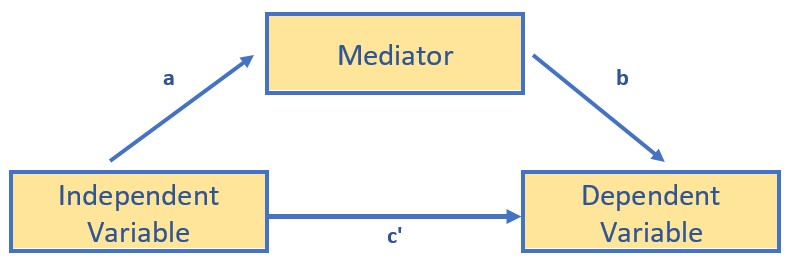
\includegraphics{images/SimpleMed/SimpleMed.jpg}
\caption{Image of Hayes'style conceptual diagram of a simple moderation}
\end{figure}

\textbf{Conditional process analysis}:

\begin{itemize}
\tightlist
\item
  Used when the research goal is to understand the boundary conditions of the mechanism(s) by which a variable transmits its effect on another.\\
\item
  Typically, simultaneously, assesses the influence of mediating (indirect effects) and moderating (interactional effects) in a model-building fashion.
\item
  In a conditional process model, the moderator(s) may be hypothesized to influence one or more of the paths.
\end{itemize}

We will work toward building a conditional process model, a moderated mediation, over the next several chapters.

\begin{figure}
\hypertarget{id}{%
\centering
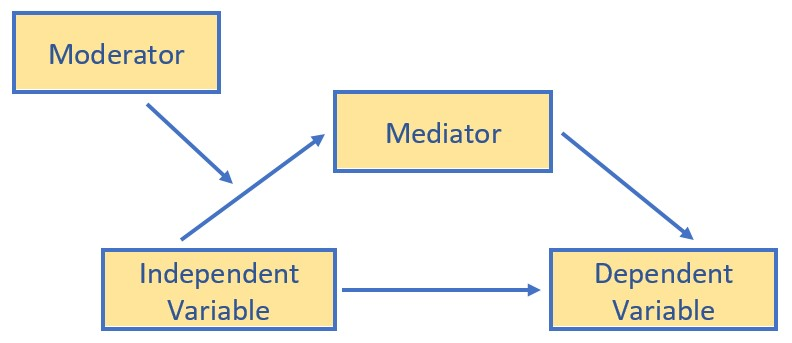
\includegraphics[width=2.60417in,height=1.875in]{images/SimpleMed/CPAmodel.jpg}
\caption{Image of conditional process analysis model where the moderator is hypothesized to change the a path; the path between the IV and mediator}\label{id}
}
\end{figure}

\hypertarget{workflow-for-simple-mediation}{%
\section{Workflow for Simple Mediation}\label{workflow-for-simple-mediation}}

The following is a proposed workflow for conducting a simple mediation.

\begin{figure}
\centering
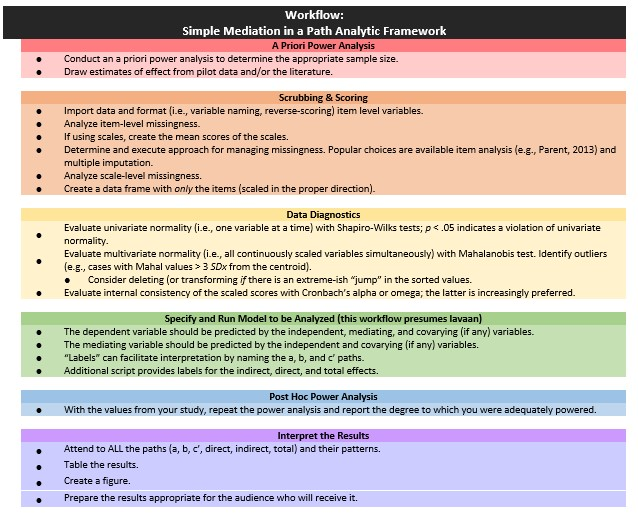
\includegraphics{images/SimpleMed/SimpMed_Workflow.jpg}
\caption{A colorful image of a workflow for the simple mediation}
\end{figure}

Conducting a simple mediation involves the following steps:

\begin{enumerate}
\def\labelenumi{\arabic{enumi}.}
\tightlist
\item
  Conducting an a priori power analysis to determine the appropriate sample size.

  \begin{itemize}
  \tightlist
  \item
    This will require estimates of effect that are drawn from pilot data, the literature, or both.
  \end{itemize}
\item
  \href{https://lhbikos.github.io/ReC_MultivModel/scrub.html}{Scrubbing} and \href{https://lhbikos.github.io/ReC_MultivModel/score.html}{scoring} the data.

  \begin{itemize}
  \tightlist
  \item
    Guidelines for such are presented in the respective lessons.
  \end{itemize}
\item
  Conducting data diagnostics, this includes:

  \begin{itemize}
  \tightlist
  \item
    item and scale level missingness,
  \item
    internal consistency coefficients (e.g., alphas or omegas) for scale scores,
  \item
    univariate and multivariate normality
  \end{itemize}
\item
  Specifying and running the model (this lesson presumes it will with the R package, \emph{lavaan}).

  \begin{itemize}
  \tightlist
  \item
    The dependent variable should be predicted by the independent, mediating, and covarying (if any) variables.
  \item
    ``Labels'' can facilitate interpretation by naming the a, b, and c' paths. +Additional script provides labels for the indirect, direct, and total effects.
  \end{itemize}
\item
  Conducting a post hoc power analysis.

  \begin{itemize}
  \tightlist
  \item
    Informed by your own results, you can see if you were adequately powered to detect a statistically significant effect, if, in fact, one exists.
  \end{itemize}
\item
  Interpret and report the results.

  \begin{itemize}
  \tightlist
  \item
    Interpret ALL the paths and their patterns.
  \item
    Create a table and figure.
  \item
    Prepare the results in a manner that is useful to your audience.
  \end{itemize}
\end{enumerate}

In addition to the workflow through the statistical problem, the very traditional and classic figure below is useful in understanding the logic beneath mediation as the explanatory mechanism.

\begin{figure}
\centering
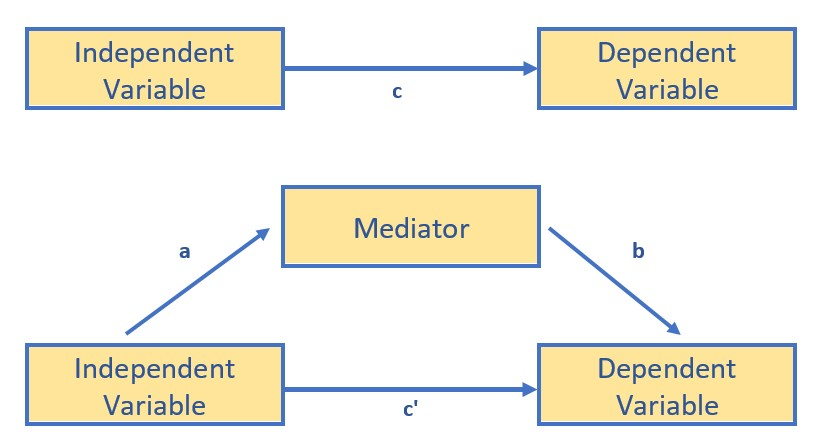
\includegraphics{images/SimpleMed/MedRationale.jpg}
\caption{Image of conditional process analysis model where the mediator is hypothesized to change the a path; the path between the IV and mediator}
\end{figure}

The top figure represents the bivariate relationship between the independent and dependent variable. The result of a simple linear regression (one predictor) represent the \emph{total} effect of the IV on the DV. We can calculate this by simply regressing the DV onto the IV. The resulting \(B\) weight is known as the \emph{c} path. A bivariate correlation coefficient results in the same value -- only it is standardized (so would be the same as the \(\beta\) weight).

The lower figure represents that the relationship between the IV and DV is \emph{mediated} by a third variable. We assign three labels to the paths: \emph{a}, between the IV and mediator; \emph{b}, between the mediator and DV; and \emph{c'} (c prime) between the IV and DV.

Although Hayes makes a compelling case that we can claim ``mediation'' when there is a statistically significant indirect effect \citeyearpar{hayes_introduction_2018}, traditionally, a mediated relationship is supported when the value of \emph{c'} is statistically significantly lower than \emph{c}. When this occurs, then know that the mediator is sharing some of the variance (and therefore acting as a \emph{conduit}) in the prediction of the DV.

You might already be imagining potential challenges to this model. For example, which variable should be the IV and which one should be the mediator? Can we switch them? You can -- and you will likely have very similar (if not identical) results. Good research design is what provides support for suggesting that mediation is the proper, casual, mechanism regarding the relationship between the IV and DV. An excellent review of the challenges of establishing a robust mediation model is provided by Kline \citeyearpar{kline_mediation_2015}, where he suggests the following as the minimally required elements of a mediation design:

\begin{itemize}
\tightlist
\item
  the IV is an experimental variable with random assignment to conditions;
\item
  the mediator is an individual difference variable that is not manipulated and is measured at a later time;and
\item
  the DV is measured at a third occasion
\end{itemize}

These criteria are in addition to the rather standard criteria for establishing causality \citep[see][ for a review]{stone-romero_research_2010}:

\begin{itemize}
\tightlist
\item
  temporal precedence,
\item
  statistical covariation, and
\item
  ruling out plausible rival hypotheses.
\end{itemize}

Some journals take this very seriously. In fact \href{https://www.journals.elsevier.com/journal-of-vocational-behavior/news/frequently-asked-questions-about-submitting-a-manuscript}{FAQs} in the Journal of Vocational Behavior make it clear that they will very rarely publish a ``mediation manuscript'' unless it has a minimum of three waves.

Working through a mediation will help operationalize these concepts.

\hypertarget{super-simple-mediation-in-lavaan-a-focus-on-the-mechanics}{%
\section{\texorpdfstring{Super Simple Mediation in \emph{lavaan}: A focus on the mechanics}{Super Simple Mediation in lavaan: A focus on the mechanics}}\label{super-simple-mediation-in-lavaan-a-focus-on-the-mechanics}}

The lavaan tutorial \citep{rosseel_lavaan_2020} provides a helpful model of how writing code to estimate an indirect effect. Using the lavaan tutorial as our guide, let's start with just a set of fake data with variable names that represent X (predictor, IV, antecedent), M (mediator, atencedent, consequent), and Y (outcome, DV, consequent).

\hypertarget{simulate-fake-data}{%
\subsection{Simulate Fake Data}\label{simulate-fake-data}}

The code below is asking to create a dataset with a sample size of 100. The dataset has 3 variables, conveniently named X (predictor, antecedent, IV), M (mediator), and Y (outome, consequent, DV). The R code asks for random selection of numbers with a normal distribution. You can see that the M variable will be related to the X variable by + .5; and the Y variable will be related to the M variable by + .7. This rather ensures a statistically significant indirect effect.

\begin{Shaded}
\begin{Highlighting}[]
\FunctionTok{set.seed}\NormalTok{(}\DecValTok{230916}\NormalTok{)}
\NormalTok{X }\OtherTok{\textless{}{-}} \FunctionTok{rnorm}\NormalTok{(}\DecValTok{100}\NormalTok{)}
\NormalTok{M }\OtherTok{\textless{}{-}} \FloatTok{0.5} \SpecialCharTok{*}\NormalTok{ X }\SpecialCharTok{+} \FunctionTok{rnorm}\NormalTok{(}\DecValTok{100}\NormalTok{)}
\NormalTok{Y }\OtherTok{\textless{}{-}} \FloatTok{0.7} \SpecialCharTok{*}\NormalTok{ M }\SpecialCharTok{+} \FunctionTok{rnorm}\NormalTok{(}\DecValTok{100}\NormalTok{)}
\NormalTok{Data }\OtherTok{\textless{}{-}} \FunctionTok{data.frame}\NormalTok{(}\AttributeTok{X =}\NormalTok{ X, }\AttributeTok{Y =}\NormalTok{ Y, }\AttributeTok{M =}\NormalTok{ M)}
\end{Highlighting}
\end{Shaded}

\hypertarget{specify-mediation-model}{%
\subsection{Specify Mediation Model}\label{specify-mediation-model}}

The package we are using is \emph{lavaan}. Hayes' model is \emph{path analysis}, which can be a form of structural equation modeling. As a quick reminder, in SPSS, PROCESS is limited to ordinary least squares regression. We will use maximum likliehood estimators for the Hayes/PROCESS examples, but \emph{lavaan} can take us further than PROCESS because

\begin{itemize}
\tightlist
\item
  We can (and, in later chapters, will) do latent variable modeling.
\item
  We can have more specificity and flexibility than the prescribed PROCESS models allow. I say this with all due respect to Hayes -- there is also a good deal of flexibility to be able to add multiple mediators and covariates within most of the Hayes' prescribed models.
\end{itemize}

Hayes text is still a great place to start because the conceptual and procedural information is clear and transferable to the R environment.

Our atheoretical dataset makes it easy to identify which variable belongs in each role (X,Y,M). When specifying the paths in lavaan, here's what to keep in mind:

\begin{itemize}
\tightlist
\item
  Name your model/object (below is X, ``\textless-'' means ``is defined by'')
\item
  The model exists between 2 single quotation marks (the odd looking ' and ' at the beginning and end).
\item
  The \# of regression equations you need depends on the \# of variables that have arrows pointing to them. In a simple mediation, there are 3 variables with 2 variables having arrows pointing to them -- need 2 regression equations:

  \begin{itemize}
  \tightlist
  \item
    one for the Mediator
  \item
    one for the DV (Y)
  \end{itemize}
\item
  Operator for a regression analysis is the (tilde, \textasciitilde)
\item
  DV goes on left

  \begin{itemize}
  \tightlist
  \item
    In first equation we regress both the X and M onto Y
  \item
    In second equation we regress M onto X
  \end{itemize}
\item
  The asterisk (*) is a handy tool to label variables (don't confuse it as defining an interaction); this labeling as a, b, and c\_p (in traditional mediation, the total effect is labeled with a and the direct effect is c'{[}c prime{]}, but the script won't allow and extra single quotation mark, hence c\_p) is super helpful in interpreting the ouput
\item
  The indirect effect is created by multiplying the a and b paths.\\
\item
  The ``:='' sign is used when creating a new variable that is a function of variables in the model, but not in the dataset (i.e., the a and b path).
\end{itemize}

After specifying the model, we create an object that holds our results from the SEM. To obtain all the results from our of indirect effects, we also need to print a summary of the fit statistics, standardized estimates, r-squared, and confidence intervals.

\emph{Other authors will write the model code more sensibly, predicting the mediator first, and then the Y variable. However, I found that by doing it this way, the semPlot produces a more sensible figure.}

Also, because we set a random seed, you should get the same results, but if it differs a little, don't panic. Also, in Hayes text the direct path from X to Y is c' (``c prime''; where as c is reserved for the total effect of X on Y).

Let's run the whole model.

\begin{Shaded}
\begin{Highlighting}[]
\NormalTok{model }\OtherTok{\textless{}{-}} \StringTok{"}
\StringTok{          Y \textasciitilde{} b*M + c\_p*X }
\StringTok{          M \textasciitilde{} a*X}
\StringTok{          }
\StringTok{          indirect :=  a*b}
\StringTok{          direct  := c\_p}
\StringTok{          total\_c  := c\_p + (a*b)}

\StringTok{          "}
\FunctionTok{set.seed}\NormalTok{(}\DecValTok{230916}\NormalTok{)  }\CommentTok{\#needed for reproducibility especially when specifying bootstrapped confidence intervals}
\NormalTok{fit }\OtherTok{\textless{}{-}}\NormalTok{ lavaan}\SpecialCharTok{::}\FunctionTok{sem}\NormalTok{(model, }\AttributeTok{data =}\NormalTok{ Data, }\AttributeTok{se =} \StringTok{"bootstrap"}\NormalTok{, }\AttributeTok{missing =} \StringTok{"fiml"}\NormalTok{)}
\NormalTok{FDsummary }\OtherTok{\textless{}{-}}\NormalTok{ lavaan}\SpecialCharTok{::}\FunctionTok{summary}\NormalTok{(fit, }\AttributeTok{standardized =}\NormalTok{ T, }\AttributeTok{rsq =}\NormalTok{ T, }\AttributeTok{fit =} \ConstantTok{TRUE}\NormalTok{,}
    \AttributeTok{ci =} \ConstantTok{TRUE}\NormalTok{)}
\NormalTok{FD\_ParamEsts }\OtherTok{\textless{}{-}}\NormalTok{ lavaan}\SpecialCharTok{::}\FunctionTok{parameterEstimates}\NormalTok{(fit, }\AttributeTok{boot.ci.type =} \StringTok{"bca.simple"}\NormalTok{,}
    \AttributeTok{standardized =} \ConstantTok{TRUE}\NormalTok{)}
\NormalTok{FDsummary}
\end{Highlighting}
\end{Shaded}

\begin{verbatim}
## lavaan 0.6.16 ended normally after 1 iteration
## 
##   Estimator                                         ML
##   Optimization method                           NLMINB
##   Number of model parameters                         7
## 
##   Number of observations                           100
##   Number of missing patterns                         1
## 
## Model Test User Model:
##                                                       
##   Test statistic                                 0.000
##   Degrees of freedom                                 0
## 
## Model Test Baseline Model:
## 
##   Test statistic                                66.380
##   Degrees of freedom                                 3
##   P-value                                        0.000
## 
## User Model versus Baseline Model:
## 
##   Comparative Fit Index (CFI)                    1.000
##   Tucker-Lewis Index (TLI)                       1.000
##                                                       
##   Robust Comparative Fit Index (CFI)             1.000
##   Robust Tucker-Lewis Index (TLI)                1.000
## 
## Loglikelihood and Information Criteria:
## 
##   Loglikelihood user model (H0)               -279.032
##   Loglikelihood unrestricted model (H1)       -279.032
##                                                       
##   Akaike (AIC)                                 572.064
##   Bayesian (BIC)                               590.301
##   Sample-size adjusted Bayesian (SABIC)        568.193
## 
## Root Mean Square Error of Approximation:
## 
##   RMSEA                                          0.000
##   90 Percent confidence interval - lower         0.000
##   90 Percent confidence interval - upper         0.000
##   P-value H_0: RMSEA <= 0.050                       NA
##   P-value H_0: RMSEA >= 0.080                       NA
##                                                       
##   Robust RMSEA                                   0.000
##   90 Percent confidence interval - lower         0.000
##   90 Percent confidence interval - upper         0.000
##   P-value H_0: Robust RMSEA <= 0.050                NA
##   P-value H_0: Robust RMSEA >= 0.080                NA
## 
## Standardized Root Mean Square Residual:
## 
##   SRMR                                           0.000
## 
## Parameter Estimates:
## 
##   Standard errors                            Bootstrap
##   Number of requested bootstrap draws             1000
##   Number of successful bootstrap draws            1000
## 
## Regressions:
##                    Estimate  Std.Err  z-value  P(>|z|) ci.lower ci.upper
##   Y ~                                                                   
##     M          (b)    0.708    0.085    8.360    0.000    0.537    0.869
##     X        (c_p)   -0.107    0.112   -0.954    0.340   -0.327    0.114
##   M ~                                                                   
##     X          (a)    0.513    0.097    5.278    0.000    0.334    0.708
##    Std.lv  Std.all
##                   
##     0.708    0.639
##    -0.107   -0.080
##                   
##     0.513    0.426
## 
## Intercepts:
##                    Estimate  Std.Err  z-value  P(>|z|) ci.lower ci.upper
##    .Y                -0.022    0.097   -0.224    0.822   -0.212    0.179
##    .M                -0.031    0.097   -0.320    0.749   -0.232    0.143
##    Std.lv  Std.all
##    -0.022   -0.018
##    -0.031   -0.028
## 
## Variances:
##                    Estimate  Std.Err  z-value  P(>|z|) ci.lower ci.upper
##    .Y                 0.927    0.127    7.315    0.000    0.669    1.160
##    .M                 0.981    0.128    7.636    0.000    0.716    1.229
##    Std.lv  Std.all
##     0.927    0.629
##     0.981    0.818
## 
## R-Square:
##                    Estimate
##     Y                 0.371
##     M                 0.182
## 
## Defined Parameters:
##                    Estimate  Std.Err  z-value  P(>|z|) ci.lower ci.upper
##     indirect          0.363    0.084    4.328    0.000    0.216    0.543
##     direct           -0.107    0.112   -0.953    0.340   -0.327    0.114
##     total_c           0.257    0.120    2.132    0.033    0.024    0.507
##    Std.lv  Std.all
##     0.363    0.272
##    -0.107   -0.080
##     0.257    0.192
\end{verbatim}

\begin{Shaded}
\begin{Highlighting}[]
\NormalTok{FD\_ParamEsts}
\end{Highlighting}
\end{Shaded}

\begin{verbatim}
##         lhs op       rhs    label    est    se      z pvalue ci.lower ci.upper
## 1         Y  ~         M        b  0.708 0.085  8.360  0.000    0.541    0.871
## 2         Y  ~         X      c_p -0.107 0.112 -0.954  0.340   -0.326    0.120
## 3         M  ~         X        a  0.513 0.097  5.278  0.000    0.332    0.705
## 4         Y ~~         Y           0.927 0.127  7.315  0.000    0.713    1.252
## 5         M ~~         M           0.981 0.128  7.636  0.000    0.766    1.282
## 6         X ~~         X           0.827 0.000     NA     NA    0.827    0.827
## 7         Y ~1                    -0.022 0.097 -0.224  0.822   -0.218    0.174
## 8         M ~1                    -0.031 0.097 -0.320  0.749   -0.210    0.183
## 9         X ~1                    -0.005 0.000     NA     NA   -0.005   -0.005
## 10 indirect :=       a*b indirect  0.363 0.084  4.328  0.000    0.224    0.557
## 11   direct :=       c_p   direct -0.107 0.112 -0.953  0.340   -0.326    0.120
## 12  total_c := c_p+(a*b)  total_c  0.257 0.120  2.132  0.033    0.029    0.517
##    std.lv std.all std.nox
## 1   0.708   0.639   0.639
## 2  -0.107  -0.080  -0.088
## 3   0.513   0.426   0.469
## 4   0.927   0.629   0.629
## 5   0.981   0.818   0.818
## 6   0.827   1.000   0.827
## 7  -0.022  -0.018  -0.018
## 8  -0.031  -0.028  -0.028
## 9  -0.005  -0.005  -0.005
## 10  0.363   0.272   0.299
## 11 -0.107  -0.080  -0.088
## 12  0.257   0.192   0.211
\end{verbatim}

\hypertarget{interpret-the-output}{%
\subsection{Interpret the Output}\label{interpret-the-output}}

Note that in the script we ask (and get) two sets of parameter estimates. The second set (in the really nice dataframe) includes bootstrapped, bias-corrected confidence intervals. Bias-corrected confidence interals have the advantage of being more powerful and bias-free. Note, though, that when the CI crosses 0, the effect is NS.

So let's look at this step-by-step.

\begin{itemize}
\tightlist
\item
  Overall, our model accounted for 37\% of the variance in the IV and 18\% of the variance in the mediator.
\item
  a path = \(B = 0.513, p < 0.001\)
\item
  b path = \(0.708, p < 0.001\)
\item
  the indirect effect is a product of the a and b paths \((0.513 * 0.708 = 0.363)\); while we don't hand calculate it's significance, we see that it is \(p < 0.001\).
\item
  the direct effect (c', c prime, or c\_p) is the isolated effect of X on Y when including M as a predictor. We hope this value is \emph{lower} than the total effect because this means that including M shared some of the variance in predicting Y: \(c' = -0.107, p = 0.340\), and it is no longer significant.
\item
  we also see the total effect; this value is

  \begin{itemize}
  \tightlist
  \item
    identical to the value of simply predicting Y on X (with no M it the model)
  \item
    the value of a(b) + c\_p: \((0.513 * 0.708) + (-0.107) = 0.257; (p = 0.033)\)
  \end{itemize}
\end{itemize}

Here's a demonstration that the total effect is, simply, predicting Y from X:

\begin{Shaded}
\begin{Highlighting}[]
\NormalTok{fitXY }\OtherTok{\textless{}{-}} \FunctionTok{lm}\NormalTok{(Y }\SpecialCharTok{\textasciitilde{}}\NormalTok{ X, }\AttributeTok{data =}\NormalTok{ Data)}
\FunctionTok{summary}\NormalTok{(fitXY)}
\end{Highlighting}
\end{Shaded}

\begin{verbatim}
## 
## Call:
## lm(formula = Y ~ X, data = Data)
## 
## Residuals:
##      Min       1Q   Median       3Q      Max 
## -2.36350 -0.90598 -0.07158  0.74879  2.52079 
## 
## Coefficients:
##             Estimate Std. Error t value Pr(>|t|)  
## (Intercept) -0.04374    0.12035  -0.363   0.7171  
## X            0.25668    0.13237   1.939   0.0554 .
## ---
## Signif. codes:  0 '***' 0.001 '**' 0.01 '*' 0.05 '.' 0.1 ' ' 1
## 
## Residual standard error: 1.204 on 98 degrees of freedom
## Multiple R-squared:  0.03695,    Adjusted R-squared:  0.02712 
## F-statistic:  3.76 on 1 and 98 DF,  p-value: 0.05537
\end{verbatim}

In a simple model such as this, it is also the same value as the bivariate correlation. The only trick is that the bivariate correlation produces a standardized result; so it would be the \(\beta\).

\begin{Shaded}
\begin{Highlighting}[]
\FunctionTok{library}\NormalTok{(psych)}
\NormalTok{XY\_r }\OtherTok{\textless{}{-}} \FunctionTok{corr.test}\NormalTok{(Data[}\FunctionTok{c}\NormalTok{(}\StringTok{"Y"}\NormalTok{, }\StringTok{"X"}\NormalTok{)])}
\NormalTok{XY\_r}
\end{Highlighting}
\end{Shaded}

\begin{verbatim}
## Call:corr.test(x = Data[c("Y", "X")])
## Correlation matrix 
##      Y    X
## Y 1.00 0.19
## X 0.19 1.00
## Sample Size 
## [1] 100
## Probability values (Entries above the diagonal are adjusted for multiple tests.) 
##      Y    X
## Y 0.00 0.06
## X 0.06 0.00
## 
##  To see confidence intervals of the correlations, print with the short=FALSE option
\end{verbatim}

\hypertarget{a-figure-and-table}{%
\subsection{A Figure and Table}\label{a-figure-and-table}}

We can use the package \href{https://cjvanlissa.github.io/tidySEM/articles/Plotting_graphs.html}{tidySEM} to create a figure that includes the values on the path.

Here's what the base package gets us

\begin{Shaded}
\begin{Highlighting}[]
\CommentTok{\# only worked when I used the library to turn on all these pkgs}
\FunctionTok{library}\NormalTok{(lavaan)}
\end{Highlighting}
\end{Shaded}

\begin{verbatim}
## This is lavaan 0.6-16
## lavaan is FREE software! Please report any bugs.
\end{verbatim}

\begin{verbatim}
## 
## Attaching package: 'lavaan'
\end{verbatim}

\begin{verbatim}
## The following object is masked from 'package:psych':
## 
##     cor2cov
\end{verbatim}

\begin{Shaded}
\begin{Highlighting}[]
\FunctionTok{library}\NormalTok{(dplyr)}
\end{Highlighting}
\end{Shaded}

\begin{verbatim}
## 
## Attaching package: 'dplyr'
\end{verbatim}

\begin{verbatim}
## The following objects are masked from 'package:stats':
## 
##     filter, lag
\end{verbatim}

\begin{verbatim}
## The following objects are masked from 'package:base':
## 
##     intersect, setdiff, setequal, union
\end{verbatim}

\begin{Shaded}
\begin{Highlighting}[]
\FunctionTok{library}\NormalTok{(ggplot2)}
\end{Highlighting}
\end{Shaded}

\begin{verbatim}
## 
## Attaching package: 'ggplot2'
\end{verbatim}

\begin{verbatim}
## The following objects are masked from 'package:psych':
## 
##     %+%, alpha
\end{verbatim}

\begin{Shaded}
\begin{Highlighting}[]
\FunctionTok{library}\NormalTok{(tidySEM)}
\end{Highlighting}
\end{Shaded}

\begin{verbatim}
## Loading required package: OpenMx
\end{verbatim}

\begin{verbatim}
## 
## Attaching package: 'OpenMx'
\end{verbatim}

\begin{verbatim}
## The following object is masked from 'package:psych':
## 
##     tr
\end{verbatim}

\begin{verbatim}
## Registered S3 method overwritten by 'tidySEM':
##   method          from  
##   predict.MxModel OpenMx
\end{verbatim}

\begin{Shaded}
\begin{Highlighting}[]
\NormalTok{tidySEM}\SpecialCharTok{::}\FunctionTok{graph\_sem}\NormalTok{(}\AttributeTok{model =}\NormalTok{ fit)}
\end{Highlighting}
\end{Shaded}

\includegraphics{05-SimpleMed_files/figure-latex/unnamed-chunk-6-1.pdf} Hayes has great examples of APA style tables that have become the standard way to communicate results. I haven't yet found a package that will turn this output into a journal-ready table, however with a little tinkering, we can approximate one of the standard tables. This code lets us understand the label names and how they are mapped

\begin{Shaded}
\begin{Highlighting}[]
\NormalTok{tidySEM}\SpecialCharTok{::}\FunctionTok{get\_layout}\NormalTok{(fit)}
\end{Highlighting}
\end{Shaded}

\begin{verbatim}
##      [,1] [,2] [,3]
## [1,] "Y"  "M"  "X" 
## attr(,"class")
## [1] "layout_matrix" "matrix"        "array"
\end{verbatim}

We can write code to remap them

\begin{Shaded}
\begin{Highlighting}[]
\NormalTok{med\_map }\OtherTok{\textless{}{-}}\NormalTok{ tidySEM}\SpecialCharTok{::}\FunctionTok{get\_layout}\NormalTok{(}\StringTok{""}\NormalTok{, }\StringTok{"M"}\NormalTok{, }\StringTok{""}\NormalTok{, }\StringTok{"X"}\NormalTok{, }\StringTok{""}\NormalTok{, }\StringTok{"Y"}\NormalTok{, }\AttributeTok{rows =} \DecValTok{2}\NormalTok{)}
\NormalTok{med\_map}
\end{Highlighting}
\end{Shaded}

\begin{verbatim}
##      [,1] [,2] [,3]
## [1,] ""   "M"  ""  
## [2,] "X"  ""   "Y" 
## attr(,"class")
## [1] "layout_matrix" "matrix"        "array"
\end{verbatim}

We run again with our map and BOOM! Still needs tinkering for gorgeous, but hey!

\begin{Shaded}
\begin{Highlighting}[]
\NormalTok{tidySEM}\SpecialCharTok{::}\FunctionTok{graph\_sem}\NormalTok{(fit, }\AttributeTok{layout =}\NormalTok{ med\_map, }\AttributeTok{rect\_width =} \FloatTok{1.5}\NormalTok{, }\AttributeTok{rect\_height =} \FloatTok{1.25}\NormalTok{,}
    \AttributeTok{spacing\_x =} \DecValTok{2}\NormalTok{, }\AttributeTok{spacing\_y =} \DecValTok{3}\NormalTok{, }\AttributeTok{text\_size =} \FloatTok{4.5}\NormalTok{)}
\end{Highlighting}
\end{Shaded}

\includegraphics{05-SimpleMed_files/figure-latex/unnamed-chunk-9-1.pdf} To assist in table preparation, it is possible to export the results to a .csv file that can be manipulated in Excel, Microsoft Word, or other program to prepare an APA style table.

\begin{Shaded}
\begin{Highlighting}[]
\FunctionTok{write.csv}\NormalTok{(FD\_ParamEsts, }\AttributeTok{file =} \StringTok{"FakeDataOUT.csv"}\NormalTok{)}
\end{Highlighting}
\end{Shaded}

Check with your discipline's journals to see how results of mediations are reported. Here's a version that I like.

Table 1

\begin{longtable}[]{@{}
  >{\raggedright\arraybackslash}p{(\columnwidth - 0\tabcolsep) * \real{1.0000}}@{}}
\toprule\noalign{}
\begin{minipage}[b]{\linewidth}\raggedright
Model Coefficients Assessing M as a Mediator Between X and Y
\end{minipage} \\
\midrule\noalign{}
\endhead
\bottomrule\noalign{}
\endlastfoot
\end{longtable}

\begin{longtable}[]{@{}
  >{\raggedright\arraybackslash}p{(\columnwidth - 6\tabcolsep) * \real{0.2809}}
  >{\centering\arraybackslash}p{(\columnwidth - 6\tabcolsep) * \real{0.3034}}
  >{\centering\arraybackslash}p{(\columnwidth - 6\tabcolsep) * \real{0.0787}}
  >{\centering\arraybackslash}p{(\columnwidth - 6\tabcolsep) * \real{0.3371}}@{}}
\toprule\noalign{}
\endhead
\bottomrule\noalign{}
\endlastfoot
& Mediator (M) & & Dependent Variable (Y) \\
\end{longtable}

\begin{longtable}[]{@{}
  >{\raggedright\arraybackslash}p{(\columnwidth - 16\tabcolsep) * \real{0.2024}}
  >{\centering\arraybackslash}p{(\columnwidth - 16\tabcolsep) * \real{0.0833}}
  >{\centering\arraybackslash}p{(\columnwidth - 16\tabcolsep) * \real{0.0952}}
  >{\centering\arraybackslash}p{(\columnwidth - 16\tabcolsep) * \real{0.0952}}
  >{\centering\arraybackslash}p{(\columnwidth - 16\tabcolsep) * \real{0.1071}}
  >{\centering\arraybackslash}p{(\columnwidth - 16\tabcolsep) * \real{0.0833}}
  >{\centering\arraybackslash}p{(\columnwidth - 16\tabcolsep) * \real{0.0952}}
  >{\centering\arraybackslash}p{(\columnwidth - 16\tabcolsep) * \real{0.1071}}
  >{\centering\arraybackslash}p{(\columnwidth - 16\tabcolsep) * \real{0.1310}}@{}}
\toprule\noalign{}
\endhead
\bottomrule\noalign{}
\endlastfoot
Antecedent & path & \(B\) & \(SE\) & \(p\) & path & \(B\) & \(SE\) & \(p\) \\
constant & \(i_{M}\) & 0.031 & 0.097 & 0.749 & \(i_{Y}\) & -0.022 & 0.097 & 0.822 \\
Independent (X) & \(a\) & 0.513 & 0.097 & \textless{} 0.001 & \(c'\) & -0.107 & 0.112 & 0.340 \\
Mediator (M) & & & & & \(b\) & 0.708 & 0.085 & \textless{} 0.0 \\
\end{longtable}

\begin{longtable}[]{@{}
  >{\raggedright\arraybackslash}p{(\columnwidth - 6\tabcolsep) * \real{0.2809}}
  >{\centering\arraybackslash}p{(\columnwidth - 6\tabcolsep) * \real{0.3034}}
  >{\centering\arraybackslash}p{(\columnwidth - 6\tabcolsep) * \real{0.0787}}
  >{\centering\arraybackslash}p{(\columnwidth - 6\tabcolsep) * \real{0.3371}}@{}}
\toprule\noalign{}
\endhead
\bottomrule\noalign{}
\endlastfoot
& \(R^2\) = 18\% & & \(R^2\) = 37\% \\
\end{longtable}

\begin{longtable}[]{@{}
  >{\raggedright\arraybackslash}p{(\columnwidth - 0\tabcolsep) * \real{1.0000}}@{}}
\toprule\noalign{}
\endhead
\bottomrule\noalign{}
\endlastfoot
\emph{Note}. The value of the indirect effect was \(B = 0.363, SE = 0.084, p < 0.001, 95CI(0.224, 0.557)\) \\
\end{longtable}

\hypertarget{results-4}{%
\subsection{Results}\label{results-4}}

A simple mediation model examined the degree to which M mediated the relation of X on Y. Using the \emph{lavaan} package (v 0.6-16) in R, coefficients for each path, the indirect effect, and total effects were calculated. These values are presented in Table 1 and illustrated in Figure 1. Results suggested that 18\% of the variance in M and 37\% of the variance in Y were accounted for in the model. The indirect effect (\(B = 0.363, SE = 0.084, p < 0.001\)) was statistically significant; the direct effect (\(B = -0.107, SE = 0.112, p = 0.340\)) was not. Comparing the nonsignificant direct effect to the statistically significant total effect (\(B = 0.257, SE = 0.120, p = 0.033\)) is consistent with the notion that the effect of X on Y is explained through M.

\hypertarget{research-vignette-4}{%
\section{Research Vignette}\label{research-vignette-4}}

The research vignette comes from the Kim, Kendall, and Cheon's \citeyearpar{kim_racial_2017}, ``Racial Microaggressions, Cultural Mistrust, and Mental Health Outcomes Among Asian American College Students.'' Participants were 156 Asian American undergraduate students in the Pacific Northwest. The researchers posited the a priori hypothesis that cultural mistrust would mediate the relationship between racial microaggressions and two sets of outcomes: mental health (e.g., depression, anxiety, well-being) and help-seeking.

Variables used in the study included:

\begin{itemize}
\tightlist
\item
  \textbf{REMS}: Racial and Ethnic Microaggressions Scale (Nadal, 2011). The scale includes 45 items on a 2-point scale where 0 indicates no experience of a microaggressive event and 1 indicates it was experienced at least once within the past six months. Higher scores indicate more experience of microaggressions.
\item
  \textbf{CMI}: Cultural Mistrust Inventory (Terrell \& Terrell, 1981). This scale was adapted to assess cultural mistrust harbored among Asian Americans toward individuals from the mainstream U.S. culture (e.g., Whites). The CMI includes 47 items on a 7-point scale where higher scores indicate a higher degree of cultural mistrust.
\item
  \textbf{ANX}, \textbf{DEP}, \textbf{PWB}: Subscales of the Mental Health Inventory (Veit \& Ware, 1983) that assess the mental health outcomes of anxiety (9 items), depression (4 items), and psychological well-being (14 items). Higher scores (on a 6 point scale) indicate stronger endorsement of the mental health outcome being assessed.
\item
  \textbf{HlpSkg}: The Attiudes Toward Seeking Professional Psychological Help -- Short Form (Fischer \& Farina, 1995) includes 10 items on a 4-point scale (0 = disagree, 3 = agree) where higher scores indicate more favorable attitudes toward help seeking.
\end{itemize}

\hypertarget{data-simulation}{%
\subsection{Data Simulation}\label{data-simulation}}

We used the \emph{lavaan::simulateData} function for the simulation. If you have taken psychometrics, you may recognize the code as one that creates latent variables form item-level data. In trying to be as authentic as possible, we retrieved factor loadings from psychometrically oriented articles that evaluated the measures \citep{nadal_racial_2011, veit_structure_1983}. For all others we specified a factor loading of 0.80. We then approximated the \emph{measurement model} by specifying the correlations between the latent variable. We sourced these from the correlation matrix from the research vignette \citep{kim_racial_2017}. The process created data with multiple decimals and values that exceeded the boundaries of the variables. For example, in all scales there were negative values. Therefore, the final element of the simulation was a linear transformation that rescaled the variables back to the range described in the journal article and rounding the values to integer (i.e., with no decimal places).

\begin{Shaded}
\begin{Highlighting}[]
\CommentTok{\# Entering the intercorrelations, means, and standard deviations from}
\CommentTok{\# the journal article}
\NormalTok{Kim\_generating\_model }\OtherTok{\textless{}{-}} \StringTok{"}
\StringTok{        \#\#measurement model}
\StringTok{         REMS =\textasciitilde{} .82*Inf32 + .75*Inf38 + .74*Inf21 + .72*Inf17 + .69*Inf9 + .61*Inf36 + .51*Inf5 + .49*Inf22 + .81*SClass6 + .81*SClass31 + .74*SClass8 + .74*SClass40 + .72*SClass2 + .65*SClass34 + .55*SClass11 + .84*mInv27 + .84*mInv30 + .80*mInv39 + .72*mInv7 + .62*mInv26 + .61*mInv33 + .53*mInv4 + .47*mInv14 + .47*mInv10 + .74*Exot3 + .74*Exot29 + .71*Exot45 + .69*Exot35 + .60*Exot42 + .59*Exot23 + .51*Exot13 + .51*Exot20 + .49*Exot43 + .84*mEnv37 + .85*mEnv24 + .78*mEnv19 + .70*mEnv28 + .69*mEnv18 + .55*mEnv41 + .55*mEnv12 + .76*mWork25 + .67*mWork15 + .65*mWork1 + .64*mWork16 + .62*mWork44}
\StringTok{         }
\StringTok{         CMI =\textasciitilde{} .8*cmi1 + .8*cmi2 + .8*cmi3 + .8*cmi4 + .8*cmi5 + .8*cmi6 + .8*cmi7 + .8*cmi8 + .8*cmi9 + .8*cmi10 + .8*cmi11 + .8*cmi12 + .8*cmi13 + .8*cmi14 + .8*cmi15 + .8*cmi16 + .8*cmi17 + .8*cmi18 + .8*cmi19 + .8*cmi20 + .8*cmi21 + .8*cmi22 + .8*cmi23 + .8*cmi24 + .8*cmi25 + .8*cmi26 + .8*cmi27 + .8*cmi28 + .8*cmi29 + .8*cmi30 + .8*cmi31 + .8*cmi32 + .8*cmi33 + .8*cmi34 + .8*cmi35 + .8*cmi36 + .8*cmi37 + .8*cmi38 + .8*cmi39 + .8*cmi40 + .8*cmi41 + .8*cmi42 + .8*cmi43 + .8*cmi44 + .8*cmi45 + .8*cmi46 + .8*cmi47}
\StringTok{         }
\StringTok{         ANX =\textasciitilde{} .80*Anx1 + .80*Anx2 + .77*Anx3 + .74*Anx4 + .74*Anx5 + .69*Anx6 + .69*Anx7 + .68*Anx8 + .50*Anx9  }
\StringTok{         DEP =\textasciitilde{} .74*Dep1 + .83*Dep2 + .82*Dep3 + .74*Dep4}
\StringTok{         PWB =\textasciitilde{} .83*pwb1 + .72*pwb2 + .67*pwb3 + .79*pwb4 + .77*pwb5 + .75*pwb6 + .74*pwb7 +.71*pwb8 +.67*pwb9 +.61*pwb10 +.58*pwb11}
\StringTok{         }
\StringTok{         HlpSkg =\textasciitilde{} .8*hlpskg1 + .8*hlpskg2 + .8*hlpskg3 + .8*hlpskg4 + .8*hlpskg5 + .8*hlpskg6 + .8*hlpskg7 + .8*hlpskg8 + .8*hlpskg9 + .8*hlpskg10 }
\StringTok{   }
\StringTok{        \# Means}
\StringTok{         REMS \textasciitilde{} 0.34*1}
\StringTok{         CMI \textasciitilde{} 3*1}
\StringTok{         ANX \textasciitilde{} 2.98*1}
\StringTok{         DEP \textasciitilde{} 2.36*1}
\StringTok{         PWB \textasciitilde{} 3.5*1}
\StringTok{         HlpSkg \textasciitilde{} 1.64*1}
\StringTok{        \# Correlations (ha!)}
\StringTok{         REMS \textasciitilde{} 0.58*CMI}
\StringTok{         REMS \textasciitilde{} 0.26*ANX}
\StringTok{         REMS \textasciitilde{} 0.34*DEP}
\StringTok{         REMS \textasciitilde{} {-}0.25*PWB}
\StringTok{         REMS \textasciitilde{} {-}0.02*HlpSkg}
\StringTok{         CMI \textasciitilde{} 0.12*ANX}
\StringTok{         CMI \textasciitilde{} 0.19*DEP}
\StringTok{         CMI \textasciitilde{} {-}0.28*PWB}
\StringTok{         CMI \textasciitilde{} 0*HlpSkg}
\StringTok{         ANX \textasciitilde{} 0.66*DEP}
\StringTok{         ANX \textasciitilde{} {-}0.55*PWB}
\StringTok{         ANX \textasciitilde{} 0.07*HlpSkg}
\StringTok{         DEP \textasciitilde{} {-}0.66*PWB}
\StringTok{         DEP \textasciitilde{} 0.05*HlpSkg}
\StringTok{         PWB \textasciitilde{} 0.08*HlpSkg}
\StringTok{        "}

\FunctionTok{set.seed}\NormalTok{(}\DecValTok{230916}\NormalTok{)}
\NormalTok{dfKim }\OtherTok{\textless{}{-}}\NormalTok{ lavaan}\SpecialCharTok{::}\FunctionTok{simulateData}\NormalTok{(}\AttributeTok{model =}\NormalTok{ Kim\_generating\_model, }\AttributeTok{model.type =} \StringTok{"sem"}\NormalTok{,}
    \AttributeTok{meanstructure =}\NormalTok{ T, }\AttributeTok{sample.nobs =} \DecValTok{156}\NormalTok{, }\AttributeTok{standardized =} \ConstantTok{FALSE}\NormalTok{)}
\FunctionTok{library}\NormalTok{(tidyverse)}
\CommentTok{\# Kim\_df\_latent \textless{}{-} Kim\_df\_latent \%\textgreater{}\% round(0) \%\textgreater{}\% abs()}

\NormalTok{dfKim}\SpecialCharTok{$}\NormalTok{Inf32 }\OtherTok{\textless{}{-}}\NormalTok{ scales}\SpecialCharTok{::}\FunctionTok{rescale}\NormalTok{(dfKim}\SpecialCharTok{$}\NormalTok{Inf32, }\FunctionTok{c}\NormalTok{(}\DecValTok{0}\NormalTok{, }\DecValTok{1}\NormalTok{))}
\NormalTok{dfKim}\SpecialCharTok{$}\NormalTok{Inf38 }\OtherTok{\textless{}{-}}\NormalTok{ scales}\SpecialCharTok{::}\FunctionTok{rescale}\NormalTok{(dfKim}\SpecialCharTok{$}\NormalTok{Inf38, }\FunctionTok{c}\NormalTok{(}\DecValTok{0}\NormalTok{, }\DecValTok{1}\NormalTok{))}
\NormalTok{dfKim}\SpecialCharTok{$}\NormalTok{Inf21 }\OtherTok{\textless{}{-}}\NormalTok{ scales}\SpecialCharTok{::}\FunctionTok{rescale}\NormalTok{(dfKim}\SpecialCharTok{$}\NormalTok{Inf21, }\FunctionTok{c}\NormalTok{(}\DecValTok{0}\NormalTok{, }\DecValTok{1}\NormalTok{))}
\NormalTok{dfKim}\SpecialCharTok{$}\NormalTok{Inf17 }\OtherTok{\textless{}{-}}\NormalTok{ scales}\SpecialCharTok{::}\FunctionTok{rescale}\NormalTok{(dfKim}\SpecialCharTok{$}\NormalTok{Inf17, }\FunctionTok{c}\NormalTok{(}\DecValTok{0}\NormalTok{, }\DecValTok{1}\NormalTok{))}
\NormalTok{dfKim}\SpecialCharTok{$}\NormalTok{Inf9 }\OtherTok{\textless{}{-}}\NormalTok{ scales}\SpecialCharTok{::}\FunctionTok{rescale}\NormalTok{(dfKim}\SpecialCharTok{$}\NormalTok{Inf9, }\FunctionTok{c}\NormalTok{(}\DecValTok{0}\NormalTok{, }\DecValTok{1}\NormalTok{))}
\NormalTok{dfKim}\SpecialCharTok{$}\NormalTok{Inf36 }\OtherTok{\textless{}{-}}\NormalTok{ scales}\SpecialCharTok{::}\FunctionTok{rescale}\NormalTok{(dfKim}\SpecialCharTok{$}\NormalTok{Inf36, }\FunctionTok{c}\NormalTok{(}\DecValTok{0}\NormalTok{, }\DecValTok{1}\NormalTok{))}
\NormalTok{dfKim}\SpecialCharTok{$}\NormalTok{Inf5 }\OtherTok{\textless{}{-}}\NormalTok{ scales}\SpecialCharTok{::}\FunctionTok{rescale}\NormalTok{(dfKim}\SpecialCharTok{$}\NormalTok{Inf5, }\FunctionTok{c}\NormalTok{(}\DecValTok{0}\NormalTok{, }\DecValTok{1}\NormalTok{))}
\NormalTok{dfKim}\SpecialCharTok{$}\NormalTok{Inf22 }\OtherTok{\textless{}{-}}\NormalTok{ scales}\SpecialCharTok{::}\FunctionTok{rescale}\NormalTok{(dfKim}\SpecialCharTok{$}\NormalTok{Inf22, }\FunctionTok{c}\NormalTok{(}\DecValTok{0}\NormalTok{, }\DecValTok{1}\NormalTok{))}
\NormalTok{dfKim}\SpecialCharTok{$}\NormalTok{SClass6 }\OtherTok{\textless{}{-}}\NormalTok{ scales}\SpecialCharTok{::}\FunctionTok{rescale}\NormalTok{(dfKim}\SpecialCharTok{$}\NormalTok{SClass6, }\FunctionTok{c}\NormalTok{(}\DecValTok{0}\NormalTok{, }\DecValTok{1}\NormalTok{))}
\NormalTok{dfKim}\SpecialCharTok{$}\NormalTok{SClass31 }\OtherTok{\textless{}{-}}\NormalTok{ scales}\SpecialCharTok{::}\FunctionTok{rescale}\NormalTok{(dfKim}\SpecialCharTok{$}\NormalTok{SClass31, }\FunctionTok{c}\NormalTok{(}\DecValTok{0}\NormalTok{, }\DecValTok{1}\NormalTok{))}
\NormalTok{dfKim}\SpecialCharTok{$}\NormalTok{SClass8 }\OtherTok{\textless{}{-}}\NormalTok{ scales}\SpecialCharTok{::}\FunctionTok{rescale}\NormalTok{(dfKim}\SpecialCharTok{$}\NormalTok{SClass8, }\FunctionTok{c}\NormalTok{(}\DecValTok{0}\NormalTok{, }\DecValTok{1}\NormalTok{))}
\NormalTok{dfKim}\SpecialCharTok{$}\NormalTok{SClass40 }\OtherTok{\textless{}{-}}\NormalTok{ scales}\SpecialCharTok{::}\FunctionTok{rescale}\NormalTok{(dfKim}\SpecialCharTok{$}\NormalTok{SClass40, }\FunctionTok{c}\NormalTok{(}\DecValTok{0}\NormalTok{, }\DecValTok{1}\NormalTok{))}
\NormalTok{dfKim}\SpecialCharTok{$}\NormalTok{SClass2 }\OtherTok{\textless{}{-}}\NormalTok{ scales}\SpecialCharTok{::}\FunctionTok{rescale}\NormalTok{(dfKim}\SpecialCharTok{$}\NormalTok{SClass2, }\FunctionTok{c}\NormalTok{(}\DecValTok{0}\NormalTok{, }\DecValTok{1}\NormalTok{))}
\NormalTok{dfKim}\SpecialCharTok{$}\NormalTok{SClass34 }\OtherTok{\textless{}{-}}\NormalTok{ scales}\SpecialCharTok{::}\FunctionTok{rescale}\NormalTok{(dfKim}\SpecialCharTok{$}\NormalTok{SClass34, }\FunctionTok{c}\NormalTok{(}\DecValTok{0}\NormalTok{, }\DecValTok{1}\NormalTok{))}
\NormalTok{dfKim}\SpecialCharTok{$}\NormalTok{SClass11 }\OtherTok{\textless{}{-}}\NormalTok{ scales}\SpecialCharTok{::}\FunctionTok{rescale}\NormalTok{(dfKim}\SpecialCharTok{$}\NormalTok{SClass11, }\FunctionTok{c}\NormalTok{(}\DecValTok{0}\NormalTok{, }\DecValTok{1}\NormalTok{))}
\NormalTok{dfKim}\SpecialCharTok{$}\NormalTok{mInv27 }\OtherTok{\textless{}{-}}\NormalTok{ scales}\SpecialCharTok{::}\FunctionTok{rescale}\NormalTok{(dfKim}\SpecialCharTok{$}\NormalTok{mInv27, }\FunctionTok{c}\NormalTok{(}\DecValTok{0}\NormalTok{, }\DecValTok{1}\NormalTok{))}
\NormalTok{dfKim}\SpecialCharTok{$}\NormalTok{mInv30 }\OtherTok{\textless{}{-}}\NormalTok{ scales}\SpecialCharTok{::}\FunctionTok{rescale}\NormalTok{(dfKim}\SpecialCharTok{$}\NormalTok{mInv30, }\FunctionTok{c}\NormalTok{(}\DecValTok{0}\NormalTok{, }\DecValTok{1}\NormalTok{))}
\NormalTok{dfKim}\SpecialCharTok{$}\NormalTok{mInv39 }\OtherTok{\textless{}{-}}\NormalTok{ scales}\SpecialCharTok{::}\FunctionTok{rescale}\NormalTok{(dfKim}\SpecialCharTok{$}\NormalTok{mInv39, }\FunctionTok{c}\NormalTok{(}\DecValTok{0}\NormalTok{, }\DecValTok{1}\NormalTok{))}
\NormalTok{dfKim}\SpecialCharTok{$}\NormalTok{mInv7 }\OtherTok{\textless{}{-}}\NormalTok{ scales}\SpecialCharTok{::}\FunctionTok{rescale}\NormalTok{(dfKim}\SpecialCharTok{$}\NormalTok{mInv7, }\FunctionTok{c}\NormalTok{(}\DecValTok{0}\NormalTok{, }\DecValTok{1}\NormalTok{))}
\NormalTok{dfKim}\SpecialCharTok{$}\NormalTok{mInv26 }\OtherTok{\textless{}{-}}\NormalTok{ scales}\SpecialCharTok{::}\FunctionTok{rescale}\NormalTok{(dfKim}\SpecialCharTok{$}\NormalTok{mInv26, }\FunctionTok{c}\NormalTok{(}\DecValTok{0}\NormalTok{, }\DecValTok{1}\NormalTok{))}
\NormalTok{dfKim}\SpecialCharTok{$}\NormalTok{mInv33 }\OtherTok{\textless{}{-}}\NormalTok{ scales}\SpecialCharTok{::}\FunctionTok{rescale}\NormalTok{(dfKim}\SpecialCharTok{$}\NormalTok{mInv33, }\FunctionTok{c}\NormalTok{(}\DecValTok{0}\NormalTok{, }\DecValTok{1}\NormalTok{))}
\NormalTok{dfKim}\SpecialCharTok{$}\NormalTok{mInv4 }\OtherTok{\textless{}{-}}\NormalTok{ scales}\SpecialCharTok{::}\FunctionTok{rescale}\NormalTok{(dfKim}\SpecialCharTok{$}\NormalTok{mInv4, }\FunctionTok{c}\NormalTok{(}\DecValTok{0}\NormalTok{, }\DecValTok{1}\NormalTok{))}
\NormalTok{dfKim}\SpecialCharTok{$}\NormalTok{mInv14 }\OtherTok{\textless{}{-}}\NormalTok{ scales}\SpecialCharTok{::}\FunctionTok{rescale}\NormalTok{(dfKim}\SpecialCharTok{$}\NormalTok{mInv14, }\FunctionTok{c}\NormalTok{(}\DecValTok{0}\NormalTok{, }\DecValTok{1}\NormalTok{))}
\NormalTok{dfKim}\SpecialCharTok{$}\NormalTok{mInv10 }\OtherTok{\textless{}{-}}\NormalTok{ scales}\SpecialCharTok{::}\FunctionTok{rescale}\NormalTok{(dfKim}\SpecialCharTok{$}\NormalTok{mInv10, }\FunctionTok{c}\NormalTok{(}\DecValTok{0}\NormalTok{, }\DecValTok{1}\NormalTok{))}
\NormalTok{dfKim}\SpecialCharTok{$}\NormalTok{Exot3 }\OtherTok{\textless{}{-}}\NormalTok{ scales}\SpecialCharTok{::}\FunctionTok{rescale}\NormalTok{(dfKim}\SpecialCharTok{$}\NormalTok{Exot3, }\FunctionTok{c}\NormalTok{(}\DecValTok{0}\NormalTok{, }\DecValTok{1}\NormalTok{))}
\NormalTok{dfKim}\SpecialCharTok{$}\NormalTok{Exot29 }\OtherTok{\textless{}{-}}\NormalTok{ scales}\SpecialCharTok{::}\FunctionTok{rescale}\NormalTok{(dfKim}\SpecialCharTok{$}\NormalTok{Exot29, }\FunctionTok{c}\NormalTok{(}\DecValTok{0}\NormalTok{, }\DecValTok{1}\NormalTok{))}
\NormalTok{dfKim}\SpecialCharTok{$}\NormalTok{Exot45 }\OtherTok{\textless{}{-}}\NormalTok{ scales}\SpecialCharTok{::}\FunctionTok{rescale}\NormalTok{(dfKim}\SpecialCharTok{$}\NormalTok{Exot45, }\FunctionTok{c}\NormalTok{(}\DecValTok{0}\NormalTok{, }\DecValTok{1}\NormalTok{))}
\NormalTok{dfKim}\SpecialCharTok{$}\NormalTok{Exot35 }\OtherTok{\textless{}{-}}\NormalTok{ scales}\SpecialCharTok{::}\FunctionTok{rescale}\NormalTok{(dfKim}\SpecialCharTok{$}\NormalTok{Exot35, }\FunctionTok{c}\NormalTok{(}\DecValTok{0}\NormalTok{, }\DecValTok{1}\NormalTok{))}
\NormalTok{dfKim}\SpecialCharTok{$}\NormalTok{Exot42 }\OtherTok{\textless{}{-}}\NormalTok{ scales}\SpecialCharTok{::}\FunctionTok{rescale}\NormalTok{(dfKim}\SpecialCharTok{$}\NormalTok{Exot42, }\FunctionTok{c}\NormalTok{(}\DecValTok{0}\NormalTok{, }\DecValTok{1}\NormalTok{))}
\NormalTok{dfKim}\SpecialCharTok{$}\NormalTok{Exot23 }\OtherTok{\textless{}{-}}\NormalTok{ scales}\SpecialCharTok{::}\FunctionTok{rescale}\NormalTok{(dfKim}\SpecialCharTok{$}\NormalTok{Exot23, }\FunctionTok{c}\NormalTok{(}\DecValTok{0}\NormalTok{, }\DecValTok{1}\NormalTok{))}
\NormalTok{dfKim}\SpecialCharTok{$}\NormalTok{Exot13 }\OtherTok{\textless{}{-}}\NormalTok{ scales}\SpecialCharTok{::}\FunctionTok{rescale}\NormalTok{(dfKim}\SpecialCharTok{$}\NormalTok{Exot13, }\FunctionTok{c}\NormalTok{(}\DecValTok{0}\NormalTok{, }\DecValTok{1}\NormalTok{))}
\NormalTok{dfKim}\SpecialCharTok{$}\NormalTok{Exot20 }\OtherTok{\textless{}{-}}\NormalTok{ scales}\SpecialCharTok{::}\FunctionTok{rescale}\NormalTok{(dfKim}\SpecialCharTok{$}\NormalTok{Exot20, }\FunctionTok{c}\NormalTok{(}\DecValTok{0}\NormalTok{, }\DecValTok{1}\NormalTok{))}
\NormalTok{dfKim}\SpecialCharTok{$}\NormalTok{Exot43 }\OtherTok{\textless{}{-}}\NormalTok{ scales}\SpecialCharTok{::}\FunctionTok{rescale}\NormalTok{(dfKim}\SpecialCharTok{$}\NormalTok{Exot43, }\FunctionTok{c}\NormalTok{(}\DecValTok{0}\NormalTok{, }\DecValTok{1}\NormalTok{))}
\NormalTok{dfKim}\SpecialCharTok{$}\NormalTok{mEnv37 }\OtherTok{\textless{}{-}}\NormalTok{ scales}\SpecialCharTok{::}\FunctionTok{rescale}\NormalTok{(dfKim}\SpecialCharTok{$}\NormalTok{mEnv37, }\FunctionTok{c}\NormalTok{(}\DecValTok{0}\NormalTok{, }\DecValTok{1}\NormalTok{))}
\NormalTok{dfKim}\SpecialCharTok{$}\NormalTok{mEnv24 }\OtherTok{\textless{}{-}}\NormalTok{ scales}\SpecialCharTok{::}\FunctionTok{rescale}\NormalTok{(dfKim}\SpecialCharTok{$}\NormalTok{mEnv24, }\FunctionTok{c}\NormalTok{(}\DecValTok{0}\NormalTok{, }\DecValTok{1}\NormalTok{))}
\NormalTok{dfKim}\SpecialCharTok{$}\NormalTok{mEnv19 }\OtherTok{\textless{}{-}}\NormalTok{ scales}\SpecialCharTok{::}\FunctionTok{rescale}\NormalTok{(dfKim}\SpecialCharTok{$}\NormalTok{mEnv19, }\FunctionTok{c}\NormalTok{(}\DecValTok{0}\NormalTok{, }\DecValTok{1}\NormalTok{))}
\NormalTok{dfKim}\SpecialCharTok{$}\NormalTok{mEnv28 }\OtherTok{\textless{}{-}}\NormalTok{ scales}\SpecialCharTok{::}\FunctionTok{rescale}\NormalTok{(dfKim}\SpecialCharTok{$}\NormalTok{mEnv28, }\FunctionTok{c}\NormalTok{(}\DecValTok{0}\NormalTok{, }\DecValTok{1}\NormalTok{))}
\NormalTok{dfKim}\SpecialCharTok{$}\NormalTok{mEnv18 }\OtherTok{\textless{}{-}}\NormalTok{ scales}\SpecialCharTok{::}\FunctionTok{rescale}\NormalTok{(dfKim}\SpecialCharTok{$}\NormalTok{mEnv18, }\FunctionTok{c}\NormalTok{(}\DecValTok{0}\NormalTok{, }\DecValTok{1}\NormalTok{))}
\NormalTok{dfKim}\SpecialCharTok{$}\NormalTok{mEnv41 }\OtherTok{\textless{}{-}}\NormalTok{ scales}\SpecialCharTok{::}\FunctionTok{rescale}\NormalTok{(dfKim}\SpecialCharTok{$}\NormalTok{mEnv41, }\FunctionTok{c}\NormalTok{(}\DecValTok{0}\NormalTok{, }\DecValTok{1}\NormalTok{))}
\NormalTok{dfKim}\SpecialCharTok{$}\NormalTok{mEnv12 }\OtherTok{\textless{}{-}}\NormalTok{ scales}\SpecialCharTok{::}\FunctionTok{rescale}\NormalTok{(dfKim}\SpecialCharTok{$}\NormalTok{mEnv12, }\FunctionTok{c}\NormalTok{(}\DecValTok{0}\NormalTok{, }\DecValTok{1}\NormalTok{))}
\NormalTok{dfKim}\SpecialCharTok{$}\NormalTok{mWork25 }\OtherTok{\textless{}{-}}\NormalTok{ scales}\SpecialCharTok{::}\FunctionTok{rescale}\NormalTok{(dfKim}\SpecialCharTok{$}\NormalTok{mWork25, }\FunctionTok{c}\NormalTok{(}\DecValTok{0}\NormalTok{, }\DecValTok{1}\NormalTok{))}
\NormalTok{dfKim}\SpecialCharTok{$}\NormalTok{mWork15 }\OtherTok{\textless{}{-}}\NormalTok{ scales}\SpecialCharTok{::}\FunctionTok{rescale}\NormalTok{(dfKim}\SpecialCharTok{$}\NormalTok{mWork15, }\FunctionTok{c}\NormalTok{(}\DecValTok{0}\NormalTok{, }\DecValTok{1}\NormalTok{))}
\NormalTok{dfKim}\SpecialCharTok{$}\NormalTok{mWork1 }\OtherTok{\textless{}{-}}\NormalTok{ scales}\SpecialCharTok{::}\FunctionTok{rescale}\NormalTok{(dfKim}\SpecialCharTok{$}\NormalTok{mWork1, }\FunctionTok{c}\NormalTok{(}\DecValTok{0}\NormalTok{, }\DecValTok{1}\NormalTok{))}
\NormalTok{dfKim}\SpecialCharTok{$}\NormalTok{mWork16 }\OtherTok{\textless{}{-}}\NormalTok{ scales}\SpecialCharTok{::}\FunctionTok{rescale}\NormalTok{(dfKim}\SpecialCharTok{$}\NormalTok{mWork16, }\FunctionTok{c}\NormalTok{(}\DecValTok{0}\NormalTok{, }\DecValTok{1}\NormalTok{))}
\NormalTok{dfKim}\SpecialCharTok{$}\NormalTok{mWork44 }\OtherTok{\textless{}{-}}\NormalTok{ scales}\SpecialCharTok{::}\FunctionTok{rescale}\NormalTok{(dfKim}\SpecialCharTok{$}\NormalTok{mWork44, }\FunctionTok{c}\NormalTok{(}\DecValTok{0}\NormalTok{, }\DecValTok{1}\NormalTok{))}

\NormalTok{dfKim}\SpecialCharTok{$}\NormalTok{cmi1 }\OtherTok{\textless{}{-}}\NormalTok{ scales}\SpecialCharTok{::}\FunctionTok{rescale}\NormalTok{(dfKim}\SpecialCharTok{$}\NormalTok{cmi1, }\FunctionTok{c}\NormalTok{(}\DecValTok{1}\NormalTok{, }\DecValTok{7}\NormalTok{))}
\NormalTok{dfKim}\SpecialCharTok{$}\NormalTok{cmi2 }\OtherTok{\textless{}{-}}\NormalTok{ scales}\SpecialCharTok{::}\FunctionTok{rescale}\NormalTok{(dfKim}\SpecialCharTok{$}\NormalTok{cmi2, }\FunctionTok{c}\NormalTok{(}\DecValTok{1}\NormalTok{, }\DecValTok{7}\NormalTok{))}
\NormalTok{dfKim}\SpecialCharTok{$}\NormalTok{cmi3 }\OtherTok{\textless{}{-}}\NormalTok{ scales}\SpecialCharTok{::}\FunctionTok{rescale}\NormalTok{(dfKim}\SpecialCharTok{$}\NormalTok{cmi3, }\FunctionTok{c}\NormalTok{(}\DecValTok{1}\NormalTok{, }\DecValTok{7}\NormalTok{))}
\NormalTok{dfKim}\SpecialCharTok{$}\NormalTok{cmi4 }\OtherTok{\textless{}{-}}\NormalTok{ scales}\SpecialCharTok{::}\FunctionTok{rescale}\NormalTok{(dfKim}\SpecialCharTok{$}\NormalTok{cmi4, }\FunctionTok{c}\NormalTok{(}\DecValTok{1}\NormalTok{, }\DecValTok{7}\NormalTok{))}
\NormalTok{dfKim}\SpecialCharTok{$}\NormalTok{cmi5 }\OtherTok{\textless{}{-}}\NormalTok{ scales}\SpecialCharTok{::}\FunctionTok{rescale}\NormalTok{(dfKim}\SpecialCharTok{$}\NormalTok{cmi5, }\FunctionTok{c}\NormalTok{(}\DecValTok{1}\NormalTok{, }\DecValTok{7}\NormalTok{))}
\NormalTok{dfKim}\SpecialCharTok{$}\NormalTok{cmi6 }\OtherTok{\textless{}{-}}\NormalTok{ scales}\SpecialCharTok{::}\FunctionTok{rescale}\NormalTok{(dfKim}\SpecialCharTok{$}\NormalTok{cmi6, }\FunctionTok{c}\NormalTok{(}\DecValTok{1}\NormalTok{, }\DecValTok{7}\NormalTok{))}
\NormalTok{dfKim}\SpecialCharTok{$}\NormalTok{cmi7 }\OtherTok{\textless{}{-}}\NormalTok{ scales}\SpecialCharTok{::}\FunctionTok{rescale}\NormalTok{(dfKim}\SpecialCharTok{$}\NormalTok{cmi7, }\FunctionTok{c}\NormalTok{(}\DecValTok{1}\NormalTok{, }\DecValTok{7}\NormalTok{))}
\NormalTok{dfKim}\SpecialCharTok{$}\NormalTok{cmi8 }\OtherTok{\textless{}{-}}\NormalTok{ scales}\SpecialCharTok{::}\FunctionTok{rescale}\NormalTok{(dfKim}\SpecialCharTok{$}\NormalTok{cmi8, }\FunctionTok{c}\NormalTok{(}\DecValTok{1}\NormalTok{, }\DecValTok{7}\NormalTok{))}
\NormalTok{dfKim}\SpecialCharTok{$}\NormalTok{cmi9 }\OtherTok{\textless{}{-}}\NormalTok{ scales}\SpecialCharTok{::}\FunctionTok{rescale}\NormalTok{(dfKim}\SpecialCharTok{$}\NormalTok{cmi9, }\FunctionTok{c}\NormalTok{(}\DecValTok{1}\NormalTok{, }\DecValTok{7}\NormalTok{))}
\NormalTok{dfKim}\SpecialCharTok{$}\NormalTok{cmi10 }\OtherTok{\textless{}{-}}\NormalTok{ scales}\SpecialCharTok{::}\FunctionTok{rescale}\NormalTok{(dfKim}\SpecialCharTok{$}\NormalTok{cmi10, }\FunctionTok{c}\NormalTok{(}\DecValTok{1}\NormalTok{, }\DecValTok{7}\NormalTok{))}
\NormalTok{dfKim}\SpecialCharTok{$}\NormalTok{cmi11 }\OtherTok{\textless{}{-}}\NormalTok{ scales}\SpecialCharTok{::}\FunctionTok{rescale}\NormalTok{(dfKim}\SpecialCharTok{$}\NormalTok{cmi11, }\FunctionTok{c}\NormalTok{(}\DecValTok{1}\NormalTok{, }\DecValTok{7}\NormalTok{))}
\NormalTok{dfKim}\SpecialCharTok{$}\NormalTok{cmi12 }\OtherTok{\textless{}{-}}\NormalTok{ scales}\SpecialCharTok{::}\FunctionTok{rescale}\NormalTok{(dfKim}\SpecialCharTok{$}\NormalTok{cmi12, }\FunctionTok{c}\NormalTok{(}\DecValTok{1}\NormalTok{, }\DecValTok{7}\NormalTok{))}
\NormalTok{dfKim}\SpecialCharTok{$}\NormalTok{cmi13 }\OtherTok{\textless{}{-}}\NormalTok{ scales}\SpecialCharTok{::}\FunctionTok{rescale}\NormalTok{(dfKim}\SpecialCharTok{$}\NormalTok{cmi13, }\FunctionTok{c}\NormalTok{(}\DecValTok{1}\NormalTok{, }\DecValTok{7}\NormalTok{))}
\NormalTok{dfKim}\SpecialCharTok{$}\NormalTok{cmi14 }\OtherTok{\textless{}{-}}\NormalTok{ scales}\SpecialCharTok{::}\FunctionTok{rescale}\NormalTok{(dfKim}\SpecialCharTok{$}\NormalTok{cmi14, }\FunctionTok{c}\NormalTok{(}\DecValTok{1}\NormalTok{, }\DecValTok{7}\NormalTok{))}
\NormalTok{dfKim}\SpecialCharTok{$}\NormalTok{cmi15 }\OtherTok{\textless{}{-}}\NormalTok{ scales}\SpecialCharTok{::}\FunctionTok{rescale}\NormalTok{(dfKim}\SpecialCharTok{$}\NormalTok{cmi15, }\FunctionTok{c}\NormalTok{(}\DecValTok{1}\NormalTok{, }\DecValTok{7}\NormalTok{))}
\NormalTok{dfKim}\SpecialCharTok{$}\NormalTok{cmi16 }\OtherTok{\textless{}{-}}\NormalTok{ scales}\SpecialCharTok{::}\FunctionTok{rescale}\NormalTok{(dfKim}\SpecialCharTok{$}\NormalTok{cmi16, }\FunctionTok{c}\NormalTok{(}\DecValTok{1}\NormalTok{, }\DecValTok{7}\NormalTok{))}
\NormalTok{dfKim}\SpecialCharTok{$}\NormalTok{cmi17 }\OtherTok{\textless{}{-}}\NormalTok{ scales}\SpecialCharTok{::}\FunctionTok{rescale}\NormalTok{(dfKim}\SpecialCharTok{$}\NormalTok{cmi17, }\FunctionTok{c}\NormalTok{(}\DecValTok{1}\NormalTok{, }\DecValTok{7}\NormalTok{))}
\NormalTok{dfKim}\SpecialCharTok{$}\NormalTok{cmi18 }\OtherTok{\textless{}{-}}\NormalTok{ scales}\SpecialCharTok{::}\FunctionTok{rescale}\NormalTok{(dfKim}\SpecialCharTok{$}\NormalTok{cmi18, }\FunctionTok{c}\NormalTok{(}\DecValTok{1}\NormalTok{, }\DecValTok{7}\NormalTok{))}
\NormalTok{dfKim}\SpecialCharTok{$}\NormalTok{cmi19 }\OtherTok{\textless{}{-}}\NormalTok{ scales}\SpecialCharTok{::}\FunctionTok{rescale}\NormalTok{(dfKim}\SpecialCharTok{$}\NormalTok{cmi19, }\FunctionTok{c}\NormalTok{(}\DecValTok{1}\NormalTok{, }\DecValTok{7}\NormalTok{))}
\NormalTok{dfKim}\SpecialCharTok{$}\NormalTok{cmi20 }\OtherTok{\textless{}{-}}\NormalTok{ scales}\SpecialCharTok{::}\FunctionTok{rescale}\NormalTok{(dfKim}\SpecialCharTok{$}\NormalTok{cmi20, }\FunctionTok{c}\NormalTok{(}\DecValTok{1}\NormalTok{, }\DecValTok{7}\NormalTok{))}
\NormalTok{dfKim}\SpecialCharTok{$}\NormalTok{cmi21 }\OtherTok{\textless{}{-}}\NormalTok{ scales}\SpecialCharTok{::}\FunctionTok{rescale}\NormalTok{(dfKim}\SpecialCharTok{$}\NormalTok{cmi21, }\FunctionTok{c}\NormalTok{(}\DecValTok{1}\NormalTok{, }\DecValTok{7}\NormalTok{))}
\NormalTok{dfKim}\SpecialCharTok{$}\NormalTok{cmi22 }\OtherTok{\textless{}{-}}\NormalTok{ scales}\SpecialCharTok{::}\FunctionTok{rescale}\NormalTok{(dfKim}\SpecialCharTok{$}\NormalTok{cmi22, }\FunctionTok{c}\NormalTok{(}\DecValTok{1}\NormalTok{, }\DecValTok{7}\NormalTok{))}
\NormalTok{dfKim}\SpecialCharTok{$}\NormalTok{cmi23 }\OtherTok{\textless{}{-}}\NormalTok{ scales}\SpecialCharTok{::}\FunctionTok{rescale}\NormalTok{(dfKim}\SpecialCharTok{$}\NormalTok{cmi23, }\FunctionTok{c}\NormalTok{(}\DecValTok{1}\NormalTok{, }\DecValTok{7}\NormalTok{))}
\NormalTok{dfKim}\SpecialCharTok{$}\NormalTok{cmi24 }\OtherTok{\textless{}{-}}\NormalTok{ scales}\SpecialCharTok{::}\FunctionTok{rescale}\NormalTok{(dfKim}\SpecialCharTok{$}\NormalTok{cmi24, }\FunctionTok{c}\NormalTok{(}\DecValTok{1}\NormalTok{, }\DecValTok{7}\NormalTok{))}
\NormalTok{dfKim}\SpecialCharTok{$}\NormalTok{cmi25 }\OtherTok{\textless{}{-}}\NormalTok{ scales}\SpecialCharTok{::}\FunctionTok{rescale}\NormalTok{(dfKim}\SpecialCharTok{$}\NormalTok{cmi25, }\FunctionTok{c}\NormalTok{(}\DecValTok{1}\NormalTok{, }\DecValTok{7}\NormalTok{))}
\NormalTok{dfKim}\SpecialCharTok{$}\NormalTok{cmi26 }\OtherTok{\textless{}{-}}\NormalTok{ scales}\SpecialCharTok{::}\FunctionTok{rescale}\NormalTok{(dfKim}\SpecialCharTok{$}\NormalTok{cmi26, }\FunctionTok{c}\NormalTok{(}\DecValTok{1}\NormalTok{, }\DecValTok{7}\NormalTok{))}
\NormalTok{dfKim}\SpecialCharTok{$}\NormalTok{cmi27 }\OtherTok{\textless{}{-}}\NormalTok{ scales}\SpecialCharTok{::}\FunctionTok{rescale}\NormalTok{(dfKim}\SpecialCharTok{$}\NormalTok{cmi27, }\FunctionTok{c}\NormalTok{(}\DecValTok{1}\NormalTok{, }\DecValTok{7}\NormalTok{))}
\NormalTok{dfKim}\SpecialCharTok{$}\NormalTok{cmi28 }\OtherTok{\textless{}{-}}\NormalTok{ scales}\SpecialCharTok{::}\FunctionTok{rescale}\NormalTok{(dfKim}\SpecialCharTok{$}\NormalTok{cmi28, }\FunctionTok{c}\NormalTok{(}\DecValTok{1}\NormalTok{, }\DecValTok{7}\NormalTok{))}
\NormalTok{dfKim}\SpecialCharTok{$}\NormalTok{cmi29 }\OtherTok{\textless{}{-}}\NormalTok{ scales}\SpecialCharTok{::}\FunctionTok{rescale}\NormalTok{(dfKim}\SpecialCharTok{$}\NormalTok{cmi29, }\FunctionTok{c}\NormalTok{(}\DecValTok{1}\NormalTok{, }\DecValTok{7}\NormalTok{))}
\NormalTok{dfKim}\SpecialCharTok{$}\NormalTok{cmi30 }\OtherTok{\textless{}{-}}\NormalTok{ scales}\SpecialCharTok{::}\FunctionTok{rescale}\NormalTok{(dfKim}\SpecialCharTok{$}\NormalTok{cmi30, }\FunctionTok{c}\NormalTok{(}\DecValTok{1}\NormalTok{, }\DecValTok{7}\NormalTok{))}
\NormalTok{dfKim}\SpecialCharTok{$}\NormalTok{cmi31 }\OtherTok{\textless{}{-}}\NormalTok{ scales}\SpecialCharTok{::}\FunctionTok{rescale}\NormalTok{(dfKim}\SpecialCharTok{$}\NormalTok{cmi31, }\FunctionTok{c}\NormalTok{(}\DecValTok{1}\NormalTok{, }\DecValTok{7}\NormalTok{))}
\NormalTok{dfKim}\SpecialCharTok{$}\NormalTok{cmi32 }\OtherTok{\textless{}{-}}\NormalTok{ scales}\SpecialCharTok{::}\FunctionTok{rescale}\NormalTok{(dfKim}\SpecialCharTok{$}\NormalTok{cmi32, }\FunctionTok{c}\NormalTok{(}\DecValTok{1}\NormalTok{, }\DecValTok{7}\NormalTok{))}
\NormalTok{dfKim}\SpecialCharTok{$}\NormalTok{cmi33 }\OtherTok{\textless{}{-}}\NormalTok{ scales}\SpecialCharTok{::}\FunctionTok{rescale}\NormalTok{(dfKim}\SpecialCharTok{$}\NormalTok{cmi33, }\FunctionTok{c}\NormalTok{(}\DecValTok{1}\NormalTok{, }\DecValTok{7}\NormalTok{))}
\NormalTok{dfKim}\SpecialCharTok{$}\NormalTok{cmi34 }\OtherTok{\textless{}{-}}\NormalTok{ scales}\SpecialCharTok{::}\FunctionTok{rescale}\NormalTok{(dfKim}\SpecialCharTok{$}\NormalTok{cmi34, }\FunctionTok{c}\NormalTok{(}\DecValTok{1}\NormalTok{, }\DecValTok{7}\NormalTok{))}
\NormalTok{dfKim}\SpecialCharTok{$}\NormalTok{cmi35 }\OtherTok{\textless{}{-}}\NormalTok{ scales}\SpecialCharTok{::}\FunctionTok{rescale}\NormalTok{(dfKim}\SpecialCharTok{$}\NormalTok{cmi35, }\FunctionTok{c}\NormalTok{(}\DecValTok{1}\NormalTok{, }\DecValTok{7}\NormalTok{))}
\NormalTok{dfKim}\SpecialCharTok{$}\NormalTok{cmi36 }\OtherTok{\textless{}{-}}\NormalTok{ scales}\SpecialCharTok{::}\FunctionTok{rescale}\NormalTok{(dfKim}\SpecialCharTok{$}\NormalTok{cmi36, }\FunctionTok{c}\NormalTok{(}\DecValTok{1}\NormalTok{, }\DecValTok{7}\NormalTok{))}
\NormalTok{dfKim}\SpecialCharTok{$}\NormalTok{cmi37 }\OtherTok{\textless{}{-}}\NormalTok{ scales}\SpecialCharTok{::}\FunctionTok{rescale}\NormalTok{(dfKim}\SpecialCharTok{$}\NormalTok{cmi37, }\FunctionTok{c}\NormalTok{(}\DecValTok{1}\NormalTok{, }\DecValTok{7}\NormalTok{))}
\NormalTok{dfKim}\SpecialCharTok{$}\NormalTok{cmi38 }\OtherTok{\textless{}{-}}\NormalTok{ scales}\SpecialCharTok{::}\FunctionTok{rescale}\NormalTok{(dfKim}\SpecialCharTok{$}\NormalTok{cmi38, }\FunctionTok{c}\NormalTok{(}\DecValTok{1}\NormalTok{, }\DecValTok{7}\NormalTok{))}
\NormalTok{dfKim}\SpecialCharTok{$}\NormalTok{cmi39 }\OtherTok{\textless{}{-}}\NormalTok{ scales}\SpecialCharTok{::}\FunctionTok{rescale}\NormalTok{(dfKim}\SpecialCharTok{$}\NormalTok{cmi39, }\FunctionTok{c}\NormalTok{(}\DecValTok{1}\NormalTok{, }\DecValTok{7}\NormalTok{))}
\NormalTok{dfKim}\SpecialCharTok{$}\NormalTok{cmi40 }\OtherTok{\textless{}{-}}\NormalTok{ scales}\SpecialCharTok{::}\FunctionTok{rescale}\NormalTok{(dfKim}\SpecialCharTok{$}\NormalTok{cmi40, }\FunctionTok{c}\NormalTok{(}\DecValTok{1}\NormalTok{, }\DecValTok{7}\NormalTok{))}
\NormalTok{dfKim}\SpecialCharTok{$}\NormalTok{cmi41 }\OtherTok{\textless{}{-}}\NormalTok{ scales}\SpecialCharTok{::}\FunctionTok{rescale}\NormalTok{(dfKim}\SpecialCharTok{$}\NormalTok{cmi41, }\FunctionTok{c}\NormalTok{(}\DecValTok{1}\NormalTok{, }\DecValTok{7}\NormalTok{))}
\NormalTok{dfKim}\SpecialCharTok{$}\NormalTok{cmi42 }\OtherTok{\textless{}{-}}\NormalTok{ scales}\SpecialCharTok{::}\FunctionTok{rescale}\NormalTok{(dfKim}\SpecialCharTok{$}\NormalTok{cmi42, }\FunctionTok{c}\NormalTok{(}\DecValTok{1}\NormalTok{, }\DecValTok{7}\NormalTok{))}
\NormalTok{dfKim}\SpecialCharTok{$}\NormalTok{cmi43 }\OtherTok{\textless{}{-}}\NormalTok{ scales}\SpecialCharTok{::}\FunctionTok{rescale}\NormalTok{(dfKim}\SpecialCharTok{$}\NormalTok{cmi43, }\FunctionTok{c}\NormalTok{(}\DecValTok{1}\NormalTok{, }\DecValTok{7}\NormalTok{))}
\NormalTok{dfKim}\SpecialCharTok{$}\NormalTok{cmi44 }\OtherTok{\textless{}{-}}\NormalTok{ scales}\SpecialCharTok{::}\FunctionTok{rescale}\NormalTok{(dfKim}\SpecialCharTok{$}\NormalTok{cmi44, }\FunctionTok{c}\NormalTok{(}\DecValTok{1}\NormalTok{, }\DecValTok{7}\NormalTok{))}
\NormalTok{dfKim}\SpecialCharTok{$}\NormalTok{cmi45 }\OtherTok{\textless{}{-}}\NormalTok{ scales}\SpecialCharTok{::}\FunctionTok{rescale}\NormalTok{(dfKim}\SpecialCharTok{$}\NormalTok{cmi45, }\FunctionTok{c}\NormalTok{(}\DecValTok{1}\NormalTok{, }\DecValTok{7}\NormalTok{))}
\NormalTok{dfKim}\SpecialCharTok{$}\NormalTok{cmi46 }\OtherTok{\textless{}{-}}\NormalTok{ scales}\SpecialCharTok{::}\FunctionTok{rescale}\NormalTok{(dfKim}\SpecialCharTok{$}\NormalTok{cmi46, }\FunctionTok{c}\NormalTok{(}\DecValTok{1}\NormalTok{, }\DecValTok{7}\NormalTok{))}
\NormalTok{dfKim}\SpecialCharTok{$}\NormalTok{cmi47 }\OtherTok{\textless{}{-}}\NormalTok{ scales}\SpecialCharTok{::}\FunctionTok{rescale}\NormalTok{(dfKim}\SpecialCharTok{$}\NormalTok{cmi47, }\FunctionTok{c}\NormalTok{(}\DecValTok{1}\NormalTok{, }\DecValTok{7}\NormalTok{))}

\NormalTok{dfKim}\SpecialCharTok{$}\NormalTok{Anx1 }\OtherTok{\textless{}{-}}\NormalTok{ scales}\SpecialCharTok{::}\FunctionTok{rescale}\NormalTok{(dfKim}\SpecialCharTok{$}\NormalTok{Anx1, }\FunctionTok{c}\NormalTok{(}\DecValTok{1}\NormalTok{, }\DecValTok{5}\NormalTok{))}
\NormalTok{dfKim}\SpecialCharTok{$}\NormalTok{Anx2 }\OtherTok{\textless{}{-}}\NormalTok{ scales}\SpecialCharTok{::}\FunctionTok{rescale}\NormalTok{(dfKim}\SpecialCharTok{$}\NormalTok{Anx2, }\FunctionTok{c}\NormalTok{(}\DecValTok{1}\NormalTok{, }\DecValTok{5}\NormalTok{))}
\NormalTok{dfKim}\SpecialCharTok{$}\NormalTok{Anx3 }\OtherTok{\textless{}{-}}\NormalTok{ scales}\SpecialCharTok{::}\FunctionTok{rescale}\NormalTok{(dfKim}\SpecialCharTok{$}\NormalTok{Anx3, }\FunctionTok{c}\NormalTok{(}\DecValTok{1}\NormalTok{, }\DecValTok{5}\NormalTok{))}
\NormalTok{dfKim}\SpecialCharTok{$}\NormalTok{Anx4 }\OtherTok{\textless{}{-}}\NormalTok{ scales}\SpecialCharTok{::}\FunctionTok{rescale}\NormalTok{(dfKim}\SpecialCharTok{$}\NormalTok{Anx4, }\FunctionTok{c}\NormalTok{(}\DecValTok{1}\NormalTok{, }\DecValTok{5}\NormalTok{))}
\NormalTok{dfKim}\SpecialCharTok{$}\NormalTok{Anx5 }\OtherTok{\textless{}{-}}\NormalTok{ scales}\SpecialCharTok{::}\FunctionTok{rescale}\NormalTok{(dfKim}\SpecialCharTok{$}\NormalTok{Anx5, }\FunctionTok{c}\NormalTok{(}\DecValTok{1}\NormalTok{, }\DecValTok{5}\NormalTok{))}
\NormalTok{dfKim}\SpecialCharTok{$}\NormalTok{Anx6 }\OtherTok{\textless{}{-}}\NormalTok{ scales}\SpecialCharTok{::}\FunctionTok{rescale}\NormalTok{(dfKim}\SpecialCharTok{$}\NormalTok{Anx6, }\FunctionTok{c}\NormalTok{(}\DecValTok{1}\NormalTok{, }\DecValTok{5}\NormalTok{))}
\NormalTok{dfKim}\SpecialCharTok{$}\NormalTok{Anx7 }\OtherTok{\textless{}{-}}\NormalTok{ scales}\SpecialCharTok{::}\FunctionTok{rescale}\NormalTok{(dfKim}\SpecialCharTok{$}\NormalTok{Anx7, }\FunctionTok{c}\NormalTok{(}\DecValTok{1}\NormalTok{, }\DecValTok{5}\NormalTok{))}
\NormalTok{dfKim}\SpecialCharTok{$}\NormalTok{Anx8 }\OtherTok{\textless{}{-}}\NormalTok{ scales}\SpecialCharTok{::}\FunctionTok{rescale}\NormalTok{(dfKim}\SpecialCharTok{$}\NormalTok{Anx8, }\FunctionTok{c}\NormalTok{(}\DecValTok{1}\NormalTok{, }\DecValTok{5}\NormalTok{))}
\NormalTok{dfKim}\SpecialCharTok{$}\NormalTok{Anx9 }\OtherTok{\textless{}{-}}\NormalTok{ scales}\SpecialCharTok{::}\FunctionTok{rescale}\NormalTok{(dfKim}\SpecialCharTok{$}\NormalTok{Anx9, }\FunctionTok{c}\NormalTok{(}\DecValTok{1}\NormalTok{, }\DecValTok{5}\NormalTok{))}

\NormalTok{dfKim}\SpecialCharTok{$}\NormalTok{Dep1 }\OtherTok{\textless{}{-}}\NormalTok{ scales}\SpecialCharTok{::}\FunctionTok{rescale}\NormalTok{(dfKim}\SpecialCharTok{$}\NormalTok{Dep1, }\FunctionTok{c}\NormalTok{(}\DecValTok{1}\NormalTok{, }\DecValTok{5}\NormalTok{))}
\NormalTok{dfKim}\SpecialCharTok{$}\NormalTok{Dep2 }\OtherTok{\textless{}{-}}\NormalTok{ scales}\SpecialCharTok{::}\FunctionTok{rescale}\NormalTok{(dfKim}\SpecialCharTok{$}\NormalTok{Dep2, }\FunctionTok{c}\NormalTok{(}\DecValTok{1}\NormalTok{, }\DecValTok{5}\NormalTok{))}
\NormalTok{dfKim}\SpecialCharTok{$}\NormalTok{Dep3 }\OtherTok{\textless{}{-}}\NormalTok{ scales}\SpecialCharTok{::}\FunctionTok{rescale}\NormalTok{(dfKim}\SpecialCharTok{$}\NormalTok{Dep3, }\FunctionTok{c}\NormalTok{(}\DecValTok{1}\NormalTok{, }\DecValTok{5}\NormalTok{))}
\NormalTok{dfKim}\SpecialCharTok{$}\NormalTok{Dep4 }\OtherTok{\textless{}{-}}\NormalTok{ scales}\SpecialCharTok{::}\FunctionTok{rescale}\NormalTok{(dfKim}\SpecialCharTok{$}\NormalTok{Dep4, }\FunctionTok{c}\NormalTok{(}\DecValTok{1}\NormalTok{, }\DecValTok{5}\NormalTok{))}

\NormalTok{dfKim}\SpecialCharTok{$}\NormalTok{pwb1 }\OtherTok{\textless{}{-}}\NormalTok{ scales}\SpecialCharTok{::}\FunctionTok{rescale}\NormalTok{(dfKim}\SpecialCharTok{$}\NormalTok{pwb1, }\FunctionTok{c}\NormalTok{(}\DecValTok{1}\NormalTok{, }\DecValTok{5}\NormalTok{))}
\NormalTok{dfKim}\SpecialCharTok{$}\NormalTok{pwb2 }\OtherTok{\textless{}{-}}\NormalTok{ scales}\SpecialCharTok{::}\FunctionTok{rescale}\NormalTok{(dfKim}\SpecialCharTok{$}\NormalTok{pwb2, }\FunctionTok{c}\NormalTok{(}\DecValTok{1}\NormalTok{, }\DecValTok{5}\NormalTok{))}
\NormalTok{dfKim}\SpecialCharTok{$}\NormalTok{pwb3 }\OtherTok{\textless{}{-}}\NormalTok{ scales}\SpecialCharTok{::}\FunctionTok{rescale}\NormalTok{(dfKim}\SpecialCharTok{$}\NormalTok{pwb3, }\FunctionTok{c}\NormalTok{(}\DecValTok{1}\NormalTok{, }\DecValTok{5}\NormalTok{))}
\NormalTok{dfKim}\SpecialCharTok{$}\NormalTok{pwb4 }\OtherTok{\textless{}{-}}\NormalTok{ scales}\SpecialCharTok{::}\FunctionTok{rescale}\NormalTok{(dfKim}\SpecialCharTok{$}\NormalTok{pwb4, }\FunctionTok{c}\NormalTok{(}\DecValTok{1}\NormalTok{, }\DecValTok{5}\NormalTok{))}
\NormalTok{dfKim}\SpecialCharTok{$}\NormalTok{pwb5 }\OtherTok{\textless{}{-}}\NormalTok{ scales}\SpecialCharTok{::}\FunctionTok{rescale}\NormalTok{(dfKim}\SpecialCharTok{$}\NormalTok{pwb5, }\FunctionTok{c}\NormalTok{(}\DecValTok{1}\NormalTok{, }\DecValTok{5}\NormalTok{))}
\NormalTok{dfKim}\SpecialCharTok{$}\NormalTok{pwb6 }\OtherTok{\textless{}{-}}\NormalTok{ scales}\SpecialCharTok{::}\FunctionTok{rescale}\NormalTok{(dfKim}\SpecialCharTok{$}\NormalTok{pwb6, }\FunctionTok{c}\NormalTok{(}\DecValTok{1}\NormalTok{, }\DecValTok{5}\NormalTok{))}
\NormalTok{dfKim}\SpecialCharTok{$}\NormalTok{pwb7 }\OtherTok{\textless{}{-}}\NormalTok{ scales}\SpecialCharTok{::}\FunctionTok{rescale}\NormalTok{(dfKim}\SpecialCharTok{$}\NormalTok{pwb7, }\FunctionTok{c}\NormalTok{(}\DecValTok{1}\NormalTok{, }\DecValTok{5}\NormalTok{))}
\NormalTok{dfKim}\SpecialCharTok{$}\NormalTok{pwb8 }\OtherTok{\textless{}{-}}\NormalTok{ scales}\SpecialCharTok{::}\FunctionTok{rescale}\NormalTok{(dfKim}\SpecialCharTok{$}\NormalTok{pwb8, }\FunctionTok{c}\NormalTok{(}\DecValTok{1}\NormalTok{, }\DecValTok{5}\NormalTok{))}
\NormalTok{dfKim}\SpecialCharTok{$}\NormalTok{pwb9 }\OtherTok{\textless{}{-}}\NormalTok{ scales}\SpecialCharTok{::}\FunctionTok{rescale}\NormalTok{(dfKim}\SpecialCharTok{$}\NormalTok{pwb9, }\FunctionTok{c}\NormalTok{(}\DecValTok{1}\NormalTok{, }\DecValTok{5}\NormalTok{))}
\NormalTok{dfKim}\SpecialCharTok{$}\NormalTok{pwb10 }\OtherTok{\textless{}{-}}\NormalTok{ scales}\SpecialCharTok{::}\FunctionTok{rescale}\NormalTok{(dfKim}\SpecialCharTok{$}\NormalTok{pwb10, }\FunctionTok{c}\NormalTok{(}\DecValTok{1}\NormalTok{, }\DecValTok{5}\NormalTok{))}
\NormalTok{dfKim}\SpecialCharTok{$}\NormalTok{pwb11 }\OtherTok{\textless{}{-}}\NormalTok{ scales}\SpecialCharTok{::}\FunctionTok{rescale}\NormalTok{(dfKim}\SpecialCharTok{$}\NormalTok{pwb11, }\FunctionTok{c}\NormalTok{(}\DecValTok{1}\NormalTok{, }\DecValTok{5}\NormalTok{))}

\NormalTok{dfKim}\SpecialCharTok{$}\NormalTok{hlpskg1 }\OtherTok{\textless{}{-}}\NormalTok{ scales}\SpecialCharTok{::}\FunctionTok{rescale}\NormalTok{(dfKim}\SpecialCharTok{$}\NormalTok{hlpskg1, }\FunctionTok{c}\NormalTok{(}\DecValTok{0}\NormalTok{, }\DecValTok{3}\NormalTok{))}
\NormalTok{dfKim}\SpecialCharTok{$}\NormalTok{hlpskg2 }\OtherTok{\textless{}{-}}\NormalTok{ scales}\SpecialCharTok{::}\FunctionTok{rescale}\NormalTok{(dfKim}\SpecialCharTok{$}\NormalTok{hlpskg2, }\FunctionTok{c}\NormalTok{(}\DecValTok{0}\NormalTok{, }\DecValTok{3}\NormalTok{))}
\NormalTok{dfKim}\SpecialCharTok{$}\NormalTok{hlpskg3 }\OtherTok{\textless{}{-}}\NormalTok{ scales}\SpecialCharTok{::}\FunctionTok{rescale}\NormalTok{(dfKim}\SpecialCharTok{$}\NormalTok{hlpskg3, }\FunctionTok{c}\NormalTok{(}\DecValTok{0}\NormalTok{, }\DecValTok{3}\NormalTok{))}
\NormalTok{dfKim}\SpecialCharTok{$}\NormalTok{hlpskg4 }\OtherTok{\textless{}{-}}\NormalTok{ scales}\SpecialCharTok{::}\FunctionTok{rescale}\NormalTok{(dfKim}\SpecialCharTok{$}\NormalTok{hlpskg4, }\FunctionTok{c}\NormalTok{(}\DecValTok{0}\NormalTok{, }\DecValTok{3}\NormalTok{))}
\NormalTok{dfKim}\SpecialCharTok{$}\NormalTok{hlpskg5 }\OtherTok{\textless{}{-}}\NormalTok{ scales}\SpecialCharTok{::}\FunctionTok{rescale}\NormalTok{(dfKim}\SpecialCharTok{$}\NormalTok{hlpskg5, }\FunctionTok{c}\NormalTok{(}\DecValTok{0}\NormalTok{, }\DecValTok{3}\NormalTok{))}
\NormalTok{dfKim}\SpecialCharTok{$}\NormalTok{hlpskg6 }\OtherTok{\textless{}{-}}\NormalTok{ scales}\SpecialCharTok{::}\FunctionTok{rescale}\NormalTok{(dfKim}\SpecialCharTok{$}\NormalTok{hlpskg6, }\FunctionTok{c}\NormalTok{(}\DecValTok{0}\NormalTok{, }\DecValTok{3}\NormalTok{))}
\NormalTok{dfKim}\SpecialCharTok{$}\NormalTok{hlpskg7 }\OtherTok{\textless{}{-}}\NormalTok{ scales}\SpecialCharTok{::}\FunctionTok{rescale}\NormalTok{(dfKim}\SpecialCharTok{$}\NormalTok{hlpskg7, }\FunctionTok{c}\NormalTok{(}\DecValTok{0}\NormalTok{, }\DecValTok{3}\NormalTok{))}
\NormalTok{dfKim}\SpecialCharTok{$}\NormalTok{hlpskg8 }\OtherTok{\textless{}{-}}\NormalTok{ scales}\SpecialCharTok{::}\FunctionTok{rescale}\NormalTok{(dfKim}\SpecialCharTok{$}\NormalTok{hlpskg8, }\FunctionTok{c}\NormalTok{(}\DecValTok{0}\NormalTok{, }\DecValTok{3}\NormalTok{))}
\NormalTok{dfKim}\SpecialCharTok{$}\NormalTok{hlpskg9 }\OtherTok{\textless{}{-}}\NormalTok{ scales}\SpecialCharTok{::}\FunctionTok{rescale}\NormalTok{(dfKim}\SpecialCharTok{$}\NormalTok{hlpskg9, }\FunctionTok{c}\NormalTok{(}\DecValTok{0}\NormalTok{, }\DecValTok{3}\NormalTok{))}
\NormalTok{dfKim}\SpecialCharTok{$}\NormalTok{hlpskg10 }\OtherTok{\textless{}{-}}\NormalTok{ scales}\SpecialCharTok{::}\FunctionTok{rescale}\NormalTok{(dfKim}\SpecialCharTok{$}\NormalTok{hlpskg10, }\FunctionTok{c}\NormalTok{(}\DecValTok{0}\NormalTok{, }\DecValTok{3}\NormalTok{))}


\CommentTok{\# psych::describe(dfKim)}

\FunctionTok{library}\NormalTok{(tidyverse)}
\NormalTok{dfKim }\OtherTok{\textless{}{-}}\NormalTok{ dfKim }\SpecialCharTok{\%\textgreater{}\%}
    \FunctionTok{round}\NormalTok{(}\DecValTok{0}\NormalTok{)}

\CommentTok{\# I tested the rescaling the correlation between original and}
\CommentTok{\# rescaled variables is 1.0 Kim\_df\_latent$INF32 \textless{}{-}}
\CommentTok{\# scales::rescale(Kim\_df\_latent$Inf32, c(0, 1))}
\CommentTok{\# cor.test(Kim\_df\_latent$Inf32, Kim\_df\_latent$INF32,}
\CommentTok{\# method=\textquotesingle{}pearson\textquotesingle{})}

\CommentTok{\# Checking our work against the original correlation matrix}
\CommentTok{\# round(cor(Kim\_df),3)}
\end{Highlighting}
\end{Shaded}

The script below allows you to store the simulated data as a file on your computer. This is optional -- the entire lesson can be worked with the simulated data.

If you prefer the .rds format, use this script (remove the hashtags). The .rds format has the advantage of preserving any formatting of variables. A disadvantage is that you cannot open these files outside of the R environment.

Script to save the data to your computer as an .rds file.

\begin{Shaded}
\begin{Highlighting}[]
\CommentTok{\#saveRDS(dfKim, \textquotesingle{}dfKim.rds\textquotesingle{})  }
\end{Highlighting}
\end{Shaded}

Once saved, you could clean your environment and bring the data back in from its .csv format.

\begin{Shaded}
\begin{Highlighting}[]
\CommentTok{\# dfKim\textless{}{-} readRDS(\textquotesingle{}dfKim.rds\textquotesingle{})}
\end{Highlighting}
\end{Shaded}

If you prefer the .csv format (think ``Excel lite'') use this script (remove the hashtags). An advantage of the .csv format is that you can open the data outside of the R environment. A disadvantage is that it may not retain any formatting of variables

Script to save the data to your computer as a .csv file.

\begin{Shaded}
\begin{Highlighting}[]
\CommentTok{\#write.table(dfKim, file = \textquotesingle{}dfKim.csv\textquotesingle{}, sep = \textquotesingle{},\textquotesingle{}, col.names=TRUE, row.names=FALSE) }
\end{Highlighting}
\end{Shaded}

Once saved, you could clean your environment and bring the data back in from its .csv format.

\begin{Shaded}
\begin{Highlighting}[]
\CommentTok{\# dfKim\textless{}{-} read.csv (\textquotesingle{}dfKim.csv\textquotesingle{}, header = TRUE)}
\end{Highlighting}
\end{Shaded}

\hypertarget{scrubbing-scoring-and-data-diagnostics}{%
\subsection{Scrubbing, Scoring, and Data Diagnostics}\label{scrubbing-scoring-and-data-diagnostics}}

Because the focus of this lesson is on simple mediation, we have used simulated data. If this were real, raw, data, it would be important to \href{https://lhbikos.github.io/ReC_MultivModel/scrub.html}{scrub}, \href{https://lhbikos.github.io/ReC_MultivModel/score.html}{score}, and conduct \href{https://lhbikos.github.io/ReC_MultivModel/DataDx.html}{data diagnostics} to evaluate the suitability of the data for the proposes anlayses.

Because we are working with item level data we first need to score the scales used in the researcher's model/. Because we are using simulated data and the authors already reverse coded any items requiring recoding, we can omit that step.

As described in the \href{https://lhbikos.github.io/ReC_MultivModel/score.html}{Scoring} chapter, we can calculate mean scores of these variables by first creating concatenated lists of variable names. Next we apply the \emph{sjstats::mean\_n} function to obtain mean scores when a given percentage (we'll specify 80\%) of variables are non-missing. We simulated a set of data that does not have missingness, none-the-less, this specification is useful in real-world settings.

\begin{Shaded}
\begin{Highlighting}[]
\NormalTok{PWB\_vars }\OtherTok{\textless{}{-}} \FunctionTok{c}\NormalTok{(}\StringTok{"pwb1"}\NormalTok{, }\StringTok{"pwb2"}\NormalTok{, }\StringTok{"pwb3"}\NormalTok{, }\StringTok{"pwb4"}\NormalTok{, }\StringTok{"pwb5"}\NormalTok{, }\StringTok{"pwb6"}\NormalTok{, }\StringTok{"pwb7"}\NormalTok{, }\StringTok{"pwb8"}\NormalTok{,}
    \StringTok{"pwb9"}\NormalTok{, }\StringTok{"pwb10"}\NormalTok{)}
\NormalTok{ANX\_vars }\OtherTok{\textless{}{-}} \FunctionTok{c}\NormalTok{(}\StringTok{"Anx1"}\NormalTok{, }\StringTok{"Anx2"}\NormalTok{, }\StringTok{"Anx3"}\NormalTok{, }\StringTok{"Anx4"}\NormalTok{, }\StringTok{"Anx5"}\NormalTok{, }\StringTok{"Anx6"}\NormalTok{, }\StringTok{"Anx7"}\NormalTok{, }\StringTok{"Anx8"}\NormalTok{,}
    \StringTok{"Anx9"}\NormalTok{)}
\NormalTok{CMI\_vars }\OtherTok{\textless{}{-}} \FunctionTok{c}\NormalTok{(}\StringTok{"cmi1"}\NormalTok{, }\StringTok{"cmi2"}\NormalTok{, }\StringTok{"cmi3"}\NormalTok{, }\StringTok{"cmi4"}\NormalTok{, }\StringTok{"cmi5"}\NormalTok{, }\StringTok{"cmi6"}\NormalTok{, }\StringTok{"cmi7"}\NormalTok{, }\StringTok{"cmi8"}\NormalTok{,}
    \StringTok{"cmi9"}\NormalTok{, }\StringTok{"cmi10"}\NormalTok{, }\StringTok{"cmi11"}\NormalTok{, }\StringTok{"cmi12"}\NormalTok{, }\StringTok{"cmi13"}\NormalTok{, }\StringTok{"cmi14"}\NormalTok{, }\StringTok{"cmi15"}\NormalTok{, }\StringTok{"cmi16"}\NormalTok{,}
    \StringTok{"cmi17"}\NormalTok{, }\StringTok{"cmi18"}\NormalTok{, }\StringTok{"cmi19"}\NormalTok{, }\StringTok{"cmi20"}\NormalTok{, }\StringTok{"cmi21"}\NormalTok{, }\StringTok{"cmi22"}\NormalTok{, }\StringTok{"cmi23"}\NormalTok{, }\StringTok{"cmi24"}\NormalTok{,}
    \StringTok{"cmi25"}\NormalTok{, }\StringTok{"cmi26"}\NormalTok{, }\StringTok{"cmi27"}\NormalTok{, }\StringTok{"cmi28"}\NormalTok{, }\StringTok{"cmi29"}\NormalTok{, }\StringTok{"cmi30"}\NormalTok{, }\StringTok{"cmi31"}\NormalTok{, }\StringTok{"cmi32"}\NormalTok{,}
    \StringTok{"cmi33"}\NormalTok{, }\StringTok{"cmi34"}\NormalTok{, }\StringTok{"cmi35"}\NormalTok{, }\StringTok{"cmi36"}\NormalTok{, }\StringTok{"cmi37"}\NormalTok{, }\StringTok{"cmi38"}\NormalTok{, }\StringTok{"cmi39"}\NormalTok{, }\StringTok{"cmi40"}\NormalTok{,}
    \StringTok{"cmi41"}\NormalTok{, }\StringTok{"cmi42"}\NormalTok{, }\StringTok{"cmi43"}\NormalTok{, }\StringTok{"cmi44"}\NormalTok{, }\StringTok{"cmi45"}\NormalTok{, }\StringTok{"cmi46"}\NormalTok{, }\StringTok{"cmi47"}\NormalTok{)}
\NormalTok{REMS\_vars }\OtherTok{\textless{}{-}} \FunctionTok{c}\NormalTok{(}\StringTok{"Inf32"}\NormalTok{, }\StringTok{"Inf38"}\NormalTok{, }\StringTok{"Inf21"}\NormalTok{, }\StringTok{"Inf17"}\NormalTok{, }\StringTok{"Inf9"}\NormalTok{, }\StringTok{"Inf36"}\NormalTok{, }\StringTok{"Inf5"}\NormalTok{,}
    \StringTok{"Inf22"}\NormalTok{, }\StringTok{"SClass6"}\NormalTok{, }\StringTok{"SClass31"}\NormalTok{, }\StringTok{"SClass8"}\NormalTok{, }\StringTok{"SClass40"}\NormalTok{, }\StringTok{"SClass2"}\NormalTok{, }\StringTok{"SClass34"}\NormalTok{,}
    \StringTok{"SClass11"}\NormalTok{, }\StringTok{"mInv27"}\NormalTok{, }\StringTok{"mInv30"}\NormalTok{, }\StringTok{"mInv39"}\NormalTok{, }\StringTok{"mInv7"}\NormalTok{, }\StringTok{"mInv26"}\NormalTok{, }\StringTok{"mInv33"}\NormalTok{,}
    \StringTok{"mInv4"}\NormalTok{, }\StringTok{"mInv14"}\NormalTok{, }\StringTok{"mInv10"}\NormalTok{, }\StringTok{"Exot3"}\NormalTok{, }\StringTok{"Exot29"}\NormalTok{, }\StringTok{"Exot45"}\NormalTok{, }\StringTok{"Exot35"}\NormalTok{,}
    \StringTok{"Exot42"}\NormalTok{, }\StringTok{"Exot23"}\NormalTok{, }\StringTok{"Exot13"}\NormalTok{, }\StringTok{"Exot20"}\NormalTok{, }\StringTok{"Exot43"}\NormalTok{, }\StringTok{"mEnv37"}\NormalTok{, }\StringTok{"mEnv24"}\NormalTok{,}
    \StringTok{"mEnv19"}\NormalTok{, }\StringTok{"mEnv28"}\NormalTok{, }\StringTok{"mEnv18"}\NormalTok{, }\StringTok{"mEnv41"}\NormalTok{, }\StringTok{"mEnv12"}\NormalTok{, }\StringTok{"mWork25"}\NormalTok{, }\StringTok{"mWork15"}\NormalTok{,}
    \StringTok{"mWork1"}\NormalTok{, }\StringTok{"mWork16"}\NormalTok{, }\StringTok{"mWork44"}\NormalTok{)}

\NormalTok{dfKim}\SpecialCharTok{$}\NormalTok{PWB }\OtherTok{\textless{}{-}}\NormalTok{ sjstats}\SpecialCharTok{::}\FunctionTok{mean\_n}\NormalTok{(dfKim[, PWB\_vars], }\FloatTok{0.8}\NormalTok{)}
\NormalTok{dfKim}\SpecialCharTok{$}\NormalTok{ANX }\OtherTok{\textless{}{-}}\NormalTok{ sjstats}\SpecialCharTok{::}\FunctionTok{mean\_n}\NormalTok{(dfKim[, ANX\_vars], }\FloatTok{0.8}\NormalTok{)}
\NormalTok{dfKim}\SpecialCharTok{$}\NormalTok{CMI }\OtherTok{\textless{}{-}}\NormalTok{ sjstats}\SpecialCharTok{::}\FunctionTok{mean\_n}\NormalTok{(dfKim[, CMI\_vars], }\FloatTok{0.8}\NormalTok{)}
\NormalTok{dfKim}\SpecialCharTok{$}\NormalTok{REMS }\OtherTok{\textless{}{-}}\NormalTok{ sjstats}\SpecialCharTok{::}\FunctionTok{mean\_n}\NormalTok{(dfKim[, REMS\_vars], }\FloatTok{0.8}\NormalTok{)}

\CommentTok{\# If the scoring code above does not work for you, try the format}
\CommentTok{\# below which involves inserting to periods in front of the variable}
\CommentTok{\# list. One example is provided. dfLewis$GRMS \textless{}{-}}
\CommentTok{\# sjstats::mean\_n(dfLewis[, ..GRMS\_vars], 0.80)}
\end{Highlighting}
\end{Shaded}

Now that we have scored our data, let's trim the variables to just those we need.

\begin{Shaded}
\begin{Highlighting}[]
\NormalTok{dfModel }\OtherTok{\textless{}{-}}\NormalTok{ dplyr}\SpecialCharTok{::}\FunctionTok{select}\NormalTok{(dfKim, PWB, ANX, CMI, REMS)}
\end{Highlighting}
\end{Shaded}

Let's check a table of means, standards, and correlations to see if they align with the published article.

\begin{Shaded}
\begin{Highlighting}[]
\NormalTok{DescriptivesTable }\OtherTok{\textless{}{-}}\NormalTok{ apaTables}\SpecialCharTok{::}\FunctionTok{apa.cor.table}\NormalTok{(dfModel, }\AttributeTok{table.number =} \DecValTok{1}\NormalTok{,}
    \AttributeTok{show.sig.stars =} \ConstantTok{TRUE}\NormalTok{, }\AttributeTok{landscape =} \ConstantTok{TRUE}\NormalTok{, }\AttributeTok{filename =} \ConstantTok{NA}\NormalTok{)}
\FunctionTok{print}\NormalTok{(DescriptivesTable)}
\end{Highlighting}
\end{Shaded}

\begin{verbatim}
## 
## 
## Table 1 
## 
## Means, standard deviations, and correlations with confidence intervals
##  
## 
##   Variable M    SD   1            2          3         
##   1. PWB   3.09 0.45                                   
##                                                        
##   2. ANX   2.82 0.57 -.50**                            
##                      [-.61, -.37]                      
##                                                        
##   3. CMI   3.94 0.77 -.49**       .43**                
##                      [-.60, -.36] [.30, .55]           
##                                                        
##   4. REMS  0.51 0.29 -.47**       .58**      .58**     
##                      [-.59, -.34] [.47, .68] [.47, .68]
##                                                        
## 
## Note. M and SD are used to represent mean and standard deviation, respectively.
## Values in square brackets indicate the 95% confidence interval.
## The confidence interval is a plausible range of population correlations 
## that could have caused the sample correlation (Cumming, 2014).
##  * indicates p < .05. ** indicates p < .01.
## 
\end{verbatim}

While the patterns are similar, we can see some differences. This means that our simulated results are likely to have some difference than the results in the published article.

\begin{longtable}[]{@{}lcc@{}}
\toprule\noalign{}
Comparison & Article & Simulation \\
\midrule\noalign{}
\endhead
\bottomrule\noalign{}
\endlastfoot
PWB mean & 3.50 & 3.09 \\
ANX mean & 2.98 & 2.82 \\
CMI mean & 3.00 & 3.94 \\
REM mean & .34 & .51 \\
PWB \textasciitilde{} ANX & -0.55*** & -0.50** \\
PWB \textasciitilde{} CMI & -0.28*** & -0.49** \\
PWB \textasciitilde{} REMS & -0.25** & -0.47** \\
ANX \textasciitilde{} CMI & 0.12 & 0.43** \\
ANX \textasciitilde{} REMS & 0.26** & 0.58** \\
CMI \textasciitilde{} REMS & 0.59*** & 0.58** \\
\end{longtable}

There are a number of reasons I love the Kim et al. \citeyearpar{kim_racial_2017} manuscript. One is that their approach was openly one that tested \emph{alternate models}. Byrne \citeyearpar{byrne_structural_2016} credits Joreskog \citep{bollen_testing_1993} with classifying the researcher's model testing approach in three ways. If a researcher uses a \emph{strictly confirmatory} approach, they only test the proposed model and then accept or reject it without further alteration. While this is the tradition of null hypothesis significance testing (NHST), it contributes to the ``file drawer problem'' of unpublished, non-significant, findings. Additionally, the data are them discarded -- potentially losing valuable resource. The \emph{alternative models} approach is to propose a handful of competing models before beginning the analysis and then evaluating to see if one model is superior to the other. The third option is \emph{model generating}. In this case the researcher begins with a theoretically proposed model. In the presence of poor fit, the researcher seeks to identify the source of misfit -- respecifying it to best represent the sample data. The researcher must use caution to produce a model that fits well and is meaningful.

Several of the Kim et al. \citeyearpar{kim_racial_2017} models were non-significant. To demonstrate a model that is statistically significant, I will test the hypothesis that racial microaggressions (REMS, the X variable) influence depression (DEP, the Y variable) through cultural mistrust (CMI, the M variable).

\begin{figure}
\centering
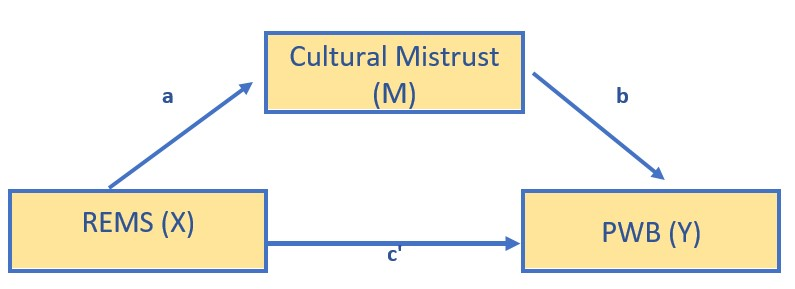
\includegraphics{images/SimpleMed/Kim_SimpMed.jpg}
\caption{Image of the simple mediation model from Kim et al.}
\end{figure}

\hypertarget{specify-the-model-in-lavaan}{%
\subsection{\texorpdfstring{Specify the Model in \emph{lavaan}}{Specify the Model in lavaan}}\label{specify-the-model-in-lavaan}}

I am a big fan of ``copying the model.'' That is, I find \emph{code that works} as a starting point. In specifying my model I used the simple mediation template from above. I

\begin{itemize}
\tightlist
\item
  replaced the Y, X, and M with variables names
\item
  replacing the name of the df
\item
  updated the object names (so I could use them in the same .rmd file)
\end{itemize}

\begin{Shaded}
\begin{Highlighting}[]
\NormalTok{modKim }\OtherTok{\textless{}{-}} \StringTok{"}
\StringTok{          PWB \textasciitilde{} b*CMI + c\_p*REMS }
\StringTok{          CMI \textasciitilde{}a*REMS}
\StringTok{          }
\StringTok{          indirect :=  a*b}
\StringTok{          direct  := c\_p}
\StringTok{          total\_c  := c\_p + (a*b)}
\StringTok{          "}
\end{Highlighting}
\end{Shaded}

\begin{Shaded}
\begin{Highlighting}[]
\FunctionTok{set.seed}\NormalTok{(}\DecValTok{230916}\NormalTok{)  }\CommentTok{\#necessary for reproducible results since lavaan introduces randomness in the estimation proces}
\NormalTok{Kim\_fit }\OtherTok{\textless{}{-}}\NormalTok{ lavaan}\SpecialCharTok{::}\FunctionTok{sem}\NormalTok{(modKim, }\AttributeTok{data =}\NormalTok{ dfModel, }\AttributeTok{se =} \StringTok{"bootstrap"}\NormalTok{, }\AttributeTok{missing =} \StringTok{"fiml"}\NormalTok{)}
\end{Highlighting}
\end{Shaded}

\begin{Shaded}
\begin{Highlighting}[]
\NormalTok{Kim\_summary }\OtherTok{\textless{}{-}} \FunctionTok{summary}\NormalTok{(Kim\_fit, }\AttributeTok{standardized =}\NormalTok{ T, }\AttributeTok{rsq =}\NormalTok{ T, }\AttributeTok{fit =} \ConstantTok{TRUE}\NormalTok{,}
    \AttributeTok{ci =} \ConstantTok{TRUE}\NormalTok{)}
\NormalTok{Kim\_ParamEsts }\OtherTok{\textless{}{-}} \FunctionTok{parameterEstimates}\NormalTok{(Kim\_fit, }\AttributeTok{boot.ci.type =} \StringTok{"bca.simple"}\NormalTok{,}
    \AttributeTok{standardized =} \ConstantTok{TRUE}\NormalTok{)}
\NormalTok{Kim\_summary}
\end{Highlighting}
\end{Shaded}

\begin{verbatim}
## lavaan 0.6.16 ended normally after 1 iteration
## 
##   Estimator                                         ML
##   Optimization method                           NLMINB
##   Number of model parameters                         7
## 
##   Number of observations                           156
##   Number of missing patterns                         1
## 
## Model Test User Model:
##                                                       
##   Test statistic                                 0.000
##   Degrees of freedom                                 0
## 
## Model Test Baseline Model:
## 
##   Test statistic                               119.320
##   Degrees of freedom                                 3
##   P-value                                        0.000
## 
## User Model versus Baseline Model:
## 
##   Comparative Fit Index (CFI)                    1.000
##   Tucker-Lewis Index (TLI)                       1.000
##                                                       
##   Robust Comparative Fit Index (CFI)             1.000
##   Robust Tucker-Lewis Index (TLI)                1.000
## 
## Loglikelihood and Information Criteria:
## 
##   Loglikelihood user model (H0)               -218.515
##   Loglikelihood unrestricted model (H1)       -218.515
##                                                       
##   Akaike (AIC)                                 451.030
##   Bayesian (BIC)                               472.379
##   Sample-size adjusted Bayesian (SABIC)        450.222
## 
## Root Mean Square Error of Approximation:
## 
##   RMSEA                                          0.000
##   90 Percent confidence interval - lower         0.000
##   90 Percent confidence interval - upper         0.000
##   P-value H_0: RMSEA <= 0.050                       NA
##   P-value H_0: RMSEA >= 0.080                       NA
##                                                       
##   Robust RMSEA                                   0.000
##   90 Percent confidence interval - lower         0.000
##   90 Percent confidence interval - upper         0.000
##   P-value H_0: Robust RMSEA <= 0.050                NA
##   P-value H_0: Robust RMSEA >= 0.080                NA
## 
## Standardized Root Mean Square Residual:
## 
##   SRMR                                           0.000
## 
## Parameter Estimates:
## 
##   Standard errors                            Bootstrap
##   Number of requested bootstrap draws             1000
##   Number of successful bootstrap draws            1000
## 
## Regressions:
##                    Estimate  Std.Err  z-value  P(>|z|) ci.lower ci.upper
##   PWB ~                                                                 
##     CMI        (b)   -0.189    0.052   -3.640    0.000   -0.291   -0.088
##     REMS     (c_p)   -0.453    0.139   -3.260    0.001   -0.740   -0.194
##   CMI ~                                                                 
##     REMS       (a)    1.576    0.177    8.920    0.000    1.199    1.938
##    Std.lv  Std.all
##                   
##    -0.189   -0.323
##    -0.453   -0.286
##                   
##     1.576    0.584
## 
## Intercepts:
##                    Estimate  Std.Err  z-value  P(>|z|) ci.lower ci.upper
##    .PWB               4.066    0.177   22.934    0.000    3.733    4.416
##    .CMI               3.141    0.104   30.276    0.000    2.933    3.364
##    Std.lv  Std.all
##     4.066    9.004
##     3.141    4.072
## 
## Variances:
##                    Estimate  Std.Err  z-value  P(>|z|) ci.lower ci.upper
##    .PWB               0.144    0.017    8.248    0.000    0.109    0.176
##    .CMI               0.392    0.041    9.557    0.000    0.312    0.473
##    Std.lv  Std.all
##     0.144    0.706
##     0.392    0.659
## 
## R-Square:
##                    Estimate
##     PWB               0.294
##     CMI               0.341
## 
## Defined Parameters:
##                    Estimate  Std.Err  z-value  P(>|z|) ci.lower ci.upper
##     indirect         -0.298    0.092   -3.251    0.001   -0.488   -0.138
##     direct           -0.453    0.139   -3.259    0.001   -0.740   -0.194
##     total_c          -0.750    0.112   -6.703    0.000   -0.961   -0.524
##    Std.lv  Std.all
##    -0.298   -0.188
##    -0.453   -0.286
##    -0.750   -0.475
\end{verbatim}

\begin{Shaded}
\begin{Highlighting}[]
\NormalTok{Kim\_ParamEsts}
\end{Highlighting}
\end{Shaded}

\begin{verbatim}
##         lhs op       rhs    label    est    se      z pvalue ci.lower ci.upper
## 1       PWB  ~       CMI        b -0.189 0.052 -3.640  0.000   -0.284   -0.081
## 2       PWB  ~      REMS      c_p -0.453 0.139 -3.260  0.001   -0.754   -0.207
## 3       CMI  ~      REMS        a  1.576 0.177  8.920  0.000    1.196    1.937
## 4       PWB ~~       PWB           0.144 0.017  8.248  0.000    0.115    0.190
## 5       CMI ~~       CMI           0.392 0.041  9.557  0.000    0.320    0.487
## 6      REMS ~~      REMS           0.082 0.000     NA     NA    0.082    0.082
## 7       PWB ~1                     4.066 0.177 22.934  0.000    3.722    4.389
## 8       CMI ~1                     3.141 0.104 30.276  0.000    2.941    3.367
## 9      REMS ~1                     0.507 0.000     NA     NA    0.507    0.507
## 10 indirect :=       a*b indirect -0.298 0.092 -3.251  0.001   -0.485   -0.131
## 11   direct :=       c_p   direct -0.453 0.139 -3.259  0.001   -0.754   -0.207
## 12  total_c := c_p+(a*b)  total_c -0.750 0.112 -6.703  0.000   -0.951   -0.518
##    std.lv std.all std.nox
## 1  -0.189  -0.323  -0.323
## 2  -0.453  -0.286  -1.002
## 3   1.576   0.584   2.043
## 4   0.144   0.706   0.706
## 5   0.392   0.659   0.659
## 6   0.082   1.000   0.082
## 7   4.066   9.004   9.004
## 8   3.141   4.072   4.072
## 9   0.507   1.775   0.507
## 10 -0.298  -0.188  -0.659
## 11 -0.453  -0.286  -1.002
## 12 -0.750  -0.475  -1.662
\end{verbatim}

\hypertarget{interpret-the-output-1}{%
\subsection{Interpret the Output}\label{interpret-the-output-1}}

\begin{itemize}
\tightlist
\item
  Overall, our model accounted for 29\% of the variance in the independent variable, well-being, and 34\% of the variance in the mediator, cultural mistrust.
\item
  a path: \(B = 1.576, p < 0.001\)
\item
  b path: \(B = -0.189, p < 0.001\)
\item
  the indirect effect is a product of the a and b paths: \(B = -0.298, p = 0.001\).
\item
  The bias-corrected bootstrapped confidence intervals can sometimes be more lenient than \(p\) values; it is important they don't cross zero \((95CI -0.485, -0.131 )\). If 0.00 is included in the confidence interval, then we cannot be confident that the estimate is not, itself, zero.
\item
  the direct effect (c', c prime, or c\_p) is the isolated effect of X on Y when including M. We hope this value is lower than the total effect because it would mean that including M shared some of the variance in predicting Y. In our case the value for \emph{c'} is: \(B = -0.453, p = 0.001\). Unfortunately, they are significant and they are not markedly different from the total effect \((B = -0.750, p < 0.001)\).
\item
  As a reminder, the total effect is is
\item
  identical to the value of simply predicting Y on X (with no M it the model)
\item
  the value of a(b) + c\_p: \((1.576*-0.189) + (-0.453) = -0.750; p < 0.001)\)
\end{itemize}

\hypertarget{a-figure-and-a-table}{%
\subsection{A Figure and a Table}\label{a-figure-and-a-table}}

I make it a practice to immediately plot what I did. Because the plotting packages use our models, this can be a helpful self-check of our work.

\begin{Shaded}
\begin{Highlighting}[]
\CommentTok{\# only worked when I used the library to turn on all these pkgs}
\FunctionTok{library}\NormalTok{(lavaan)}
\FunctionTok{library}\NormalTok{(dplyr)}
\FunctionTok{library}\NormalTok{(ggplot2)}
\FunctionTok{library}\NormalTok{(tidySEM)}
\NormalTok{tidySEM}\SpecialCharTok{::}\FunctionTok{graph\_sem}\NormalTok{(}\AttributeTok{model =}\NormalTok{ Kim\_fit)}
\end{Highlighting}
\end{Shaded}

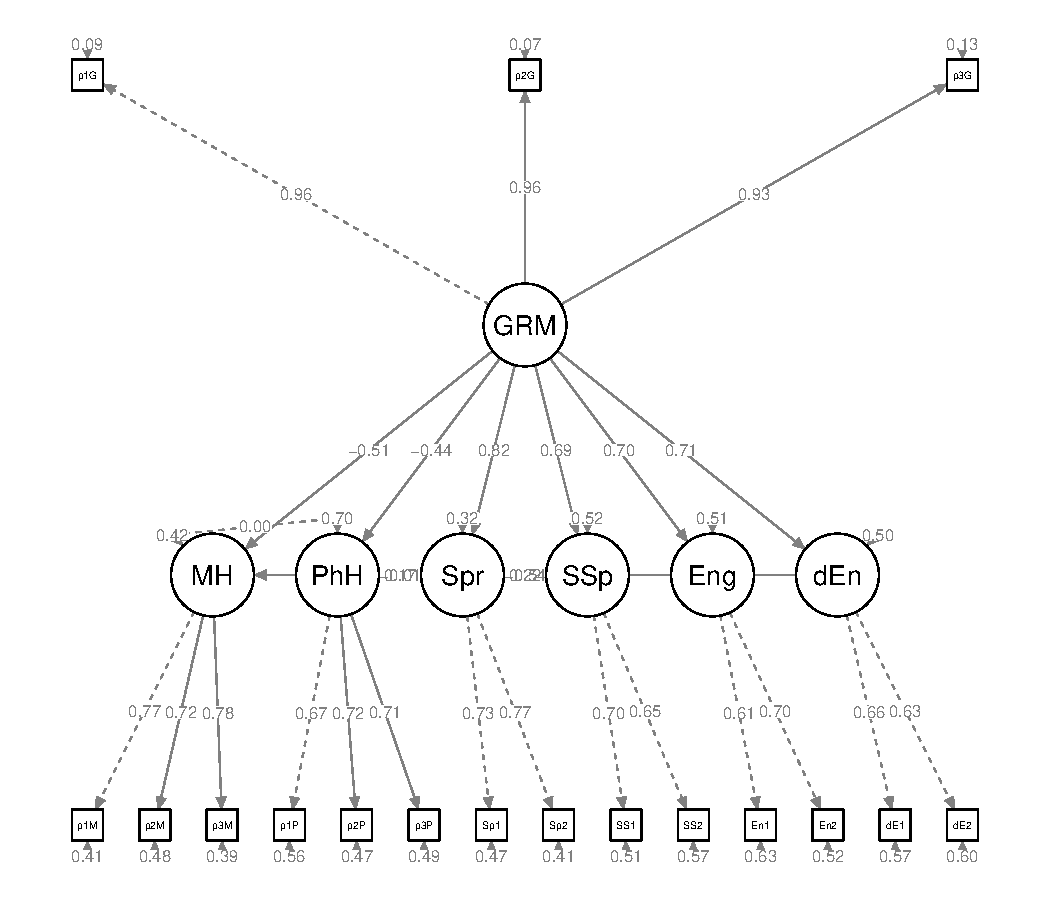
\includegraphics{05-SimpleMed_files/figure-latex/unnamed-chunk-22-1.pdf} Hayes has great examples of APA style tables that have become the standard way to communicate results. I haven't yet found a package that will turn this output into a journal-ready table, however with a little tinkering, we can approximate one of the standard tables. This code lets us understand the label names and how they are mapped

\begin{Shaded}
\begin{Highlighting}[]
\NormalTok{tidySEM}\SpecialCharTok{::}\FunctionTok{get\_layout}\NormalTok{(Kim\_fit)}
\end{Highlighting}
\end{Shaded}

\begin{verbatim}
##      [,1]  [,2]  
## [1,] NA    "REMS"
## [2,] "PWB" "CMI" 
## attr(,"class")
## [1] "layout_matrix" "matrix"        "array"
\end{verbatim}

We can write code to remap them

\begin{Shaded}
\begin{Highlighting}[]
\NormalTok{med\_map2 }\OtherTok{\textless{}{-}}\NormalTok{ tidySEM}\SpecialCharTok{::}\FunctionTok{get\_layout}\NormalTok{(}\StringTok{""}\NormalTok{, }\StringTok{"CMI"}\NormalTok{, }\StringTok{""}\NormalTok{, }\StringTok{"REMS"}\NormalTok{, }\StringTok{""}\NormalTok{, }\StringTok{"PWB"}\NormalTok{, }\AttributeTok{rows =} \DecValTok{2}\NormalTok{)}
\NormalTok{med\_map2}
\end{Highlighting}
\end{Shaded}

\begin{verbatim}
##      [,1]   [,2]  [,3] 
## [1,] ""     "CMI" ""   
## [2,] "REMS" ""    "PWB"
## attr(,"class")
## [1] "layout_matrix" "matrix"        "array"
\end{verbatim}

We run again with our map and BOOM! Still needs tinkering for gorgeous, but hey!

\begin{Shaded}
\begin{Highlighting}[]
\NormalTok{tidySEM}\SpecialCharTok{::}\FunctionTok{graph\_sem}\NormalTok{(Kim\_fit, }\AttributeTok{layout =}\NormalTok{ med\_map2, }\AttributeTok{rect\_width =} \FloatTok{1.5}\NormalTok{, }\AttributeTok{rect\_height =} \FloatTok{1.25}\NormalTok{,}
    \AttributeTok{spacing\_x =} \DecValTok{2}\NormalTok{, }\AttributeTok{spacing\_y =} \DecValTok{3}\NormalTok{, }\AttributeTok{text\_size =} \FloatTok{4.5}\NormalTok{)}
\end{Highlighting}
\end{Shaded}

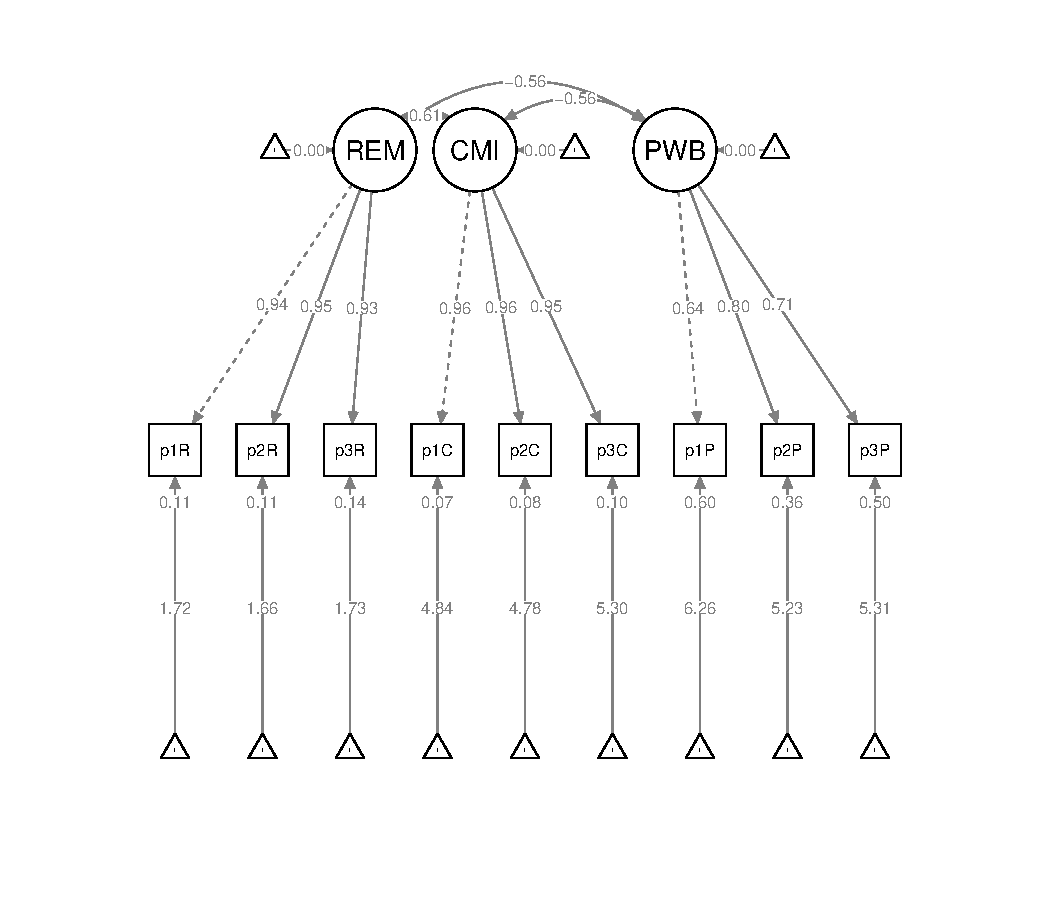
\includegraphics{05-SimpleMed_files/figure-latex/unnamed-chunk-25-1.pdf}

We can use simple code from base R to write the results to a .csv file. This makes it easier to create a table for presenting the results.

\begin{Shaded}
\begin{Highlighting}[]
\FunctionTok{write.csv}\NormalTok{(Kim\_ParamEsts, }\AttributeTok{file =} \StringTok{"KimSimpleMed.csv"}\NormalTok{)}
\end{Highlighting}
\end{Shaded}

Here's how I might organize the data.

Table 2

\begin{longtable}[]{@{}
  >{\raggedright\arraybackslash}p{(\columnwidth - 0\tabcolsep) * \real{1.0000}}@{}}
\toprule\noalign{}
\begin{minipage}[b]{\linewidth}\raggedright
Model Coefficients Assessing Cultural Mistrust as a Mediator Between Racial Microaggressions and Well-Being
\end{minipage} \\
\midrule\noalign{}
\endhead
\bottomrule\noalign{}
\endlastfoot
\end{longtable}

\begin{longtable}[]{@{}
  >{\raggedright\arraybackslash}p{(\columnwidth - 6\tabcolsep) * \real{0.2292}}
  >{\centering\arraybackslash}p{(\columnwidth - 6\tabcolsep) * \real{0.2812}}
  >{\centering\arraybackslash}p{(\columnwidth - 6\tabcolsep) * \real{0.0729}}
  >{\centering\arraybackslash}p{(\columnwidth - 6\tabcolsep) * \real{0.4167}}@{}}
\toprule\noalign{}
\endhead
\bottomrule\noalign{}
\endlastfoot
& Cultural Mistrust (M) & & Well-Being (Y) \\
\end{longtable}

\begin{longtable}[]{@{}
  >{\raggedright\arraybackslash}p{(\columnwidth - 16\tabcolsep) * \real{0.1538}}
  >{\centering\arraybackslash}p{(\columnwidth - 16\tabcolsep) * \real{0.0769}}
  >{\centering\arraybackslash}p{(\columnwidth - 16\tabcolsep) * \real{0.0879}}
  >{\centering\arraybackslash}p{(\columnwidth - 16\tabcolsep) * \real{0.0769}}
  >{\centering\arraybackslash}p{(\columnwidth - 16\tabcolsep) * \real{0.1099}}
  >{\centering\arraybackslash}p{(\columnwidth - 16\tabcolsep) * \real{0.0769}}
  >{\centering\arraybackslash}p{(\columnwidth - 16\tabcolsep) * \real{0.1209}}
  >{\centering\arraybackslash}p{(\columnwidth - 16\tabcolsep) * \real{0.1538}}
  >{\centering\arraybackslash}p{(\columnwidth - 16\tabcolsep) * \real{0.1429}}@{}}
\toprule\noalign{}
\endhead
\bottomrule\noalign{}
\endlastfoot
Antecedent & path & \(B\) & \(SE\) & \(p\) & path & \(B\) & \(SE\) & \(p\) \\
constant & \(i_{M}\) & 3.1419 & 0.103 & \textless{} 0.001 & \(i_{Y}\) & 4.066 & 0.177 & \textless{} 0.001 \\
REMS (X) & \(a\) & 1.576 & 0.184 & \textless{} 0.001 & \(c'\) & -0.453 & 0.139 & 0.001 \\
CMI (M) & & & & & \(b\) & -0.189 & 0.052 & \textless{} 0.001 \\
\end{longtable}

\begin{longtable}[]{@{}
  >{\raggedright\arraybackslash}p{(\columnwidth - 6\tabcolsep) * \real{0.2292}}
  >{\centering\arraybackslash}p{(\columnwidth - 6\tabcolsep) * \real{0.2812}}
  >{\centering\arraybackslash}p{(\columnwidth - 6\tabcolsep) * \real{0.0729}}
  >{\centering\arraybackslash}p{(\columnwidth - 6\tabcolsep) * \real{0.4167}}@{}}
\toprule\noalign{}
\endhead
\bottomrule\noalign{}
\endlastfoot
& \(R^2\) = 34\% & & \(R^2\) = 29\% \\
\end{longtable}

\begin{longtable}[]{@{}
  >{\raggedright\arraybackslash}p{(\columnwidth - 0\tabcolsep) * \real{1.0000}}@{}}
\toprule\noalign{}
\endhead
\bottomrule\noalign{}
\endlastfoot
\emph{Note}. The value of the indirect effect was \(B = -.298, SE = 0.092, p = 0.001, 95CI(-0.485,-0.131)\). \\
\end{longtable}

\hypertarget{results-5}{%
\subsection{Results}\label{results-5}}

A simple mediation model examined the degree to which cultural mistrust mediated the relation of racial microaggressions on well-being. Using the \emph{lavaan} package (v 0.6-16) in R, coefficients for each path, the indirect effect, and total effects were calculated. These values are presented in Table 2 and illustrated in Figure 2. Results suggested that racial/ethnic microaggressions had statistically significant effects on both cultural mistrust \((B = 1.576, p < 0.001)\) and well-being \((B = -0.453, p = 0.001)\). Further, the indirect effect from our simulated data was statistically significant (\(B = -.298, SE = 0.092, p = 0.001, 95CI[-0.485,-0.131])\). Results suggested that 34\% of the variance in cultural mistrust and 29\% of the variance in well-being were accounted for by the model.

\hypertarget{considering-covariates}{%
\section{Considering Covariates}\label{considering-covariates}}

Hayes Chapter 4 \citeyearpar{hayes_introduction_2018} considers the role of covariates (e.g., other variables that could account for some of the variance in the model). When previous research (or commonsense, or detractors) suggest you should include them it is advisable to do so. If they are non-significant and/or your variables continue to explain variance over-and-above their contribution, then you have gained ground in ruling out plausible rival hypotheses and are adding to causal evidence.

Covariates are relatively easy to specify in \emph{lavaan}. I tend to look at my figure and ``see where the arrows go.'' Those translate readily to the equations we write in the \emph{lavaan} code.

Let's say we are concerned that anxiety covaries with cultural mistrust and well-being We'll add it as a covariate to both.

\begin{figure}
\centering
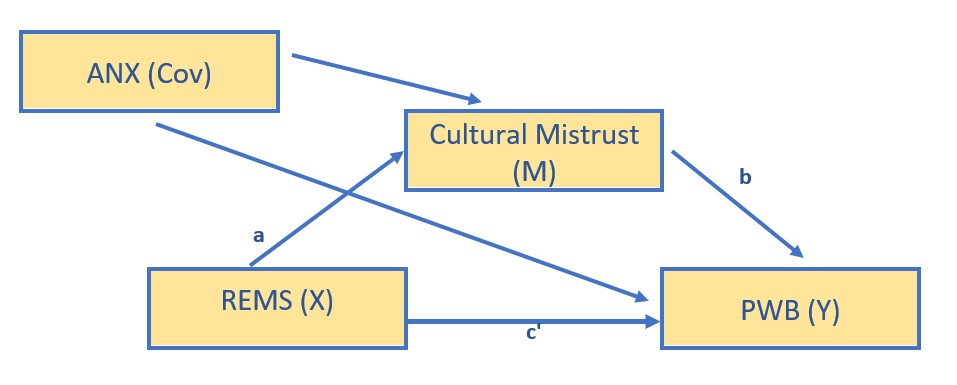
\includegraphics{images/SimpleMed/Kim_wCovs.jpg}
\caption{Image of the simple mediation model from Kim et al.}
\end{figure}

\begin{Shaded}
\begin{Highlighting}[]
\NormalTok{Kim\_fit\_covs }\OtherTok{\textless{}{-}} \StringTok{"}
\StringTok{          PWB \textasciitilde{} b*CMI + c\_p*REMS }
\StringTok{          CMI \textasciitilde{}a*REMS}
\StringTok{          CMI \textasciitilde{} covM*ANX}
\StringTok{          PWB \textasciitilde{} covY*ANX}

\StringTok{          indirect :=  a*b}
\StringTok{          direct  := c\_p}
\StringTok{          total\_c  := c\_p + (a*b)}

\StringTok{          "}
\FunctionTok{set.seed}\NormalTok{(}\DecValTok{230916}\NormalTok{)  }\CommentTok{\#needed for reproducibility especially when specifying bootstrapped confidence intervals}
\NormalTok{Kim\_fit\_covs }\OtherTok{\textless{}{-}}\NormalTok{ lavaan}\SpecialCharTok{::}\FunctionTok{sem}\NormalTok{(Kim\_fit\_covs, }\AttributeTok{data =}\NormalTok{ dfKim, }\AttributeTok{se =} \StringTok{"bootstrap"}\NormalTok{,}
    \AttributeTok{missing =} \StringTok{"fiml"}\NormalTok{)}
\NormalTok{Kcov\_sum }\OtherTok{\textless{}{-}}\NormalTok{ lavaan}\SpecialCharTok{::}\FunctionTok{summary}\NormalTok{(Kim\_fit\_covs, }\AttributeTok{standardized =}\NormalTok{ T, }\AttributeTok{rsq =}\NormalTok{ T, }\AttributeTok{fit =} \ConstantTok{TRUE}\NormalTok{,}
    \AttributeTok{ci =} \ConstantTok{TRUE}\NormalTok{)}
\NormalTok{Kcov\_ParEsts }\OtherTok{\textless{}{-}}\NormalTok{ lavaan}\SpecialCharTok{::}\FunctionTok{parameterEstimates}\NormalTok{(Kim\_fit\_covs, }\AttributeTok{boot.ci.type =} \StringTok{"bca.simple"}\NormalTok{,}
    \AttributeTok{standardized =} \ConstantTok{TRUE}\NormalTok{)}
\NormalTok{Kcov\_sum}
\end{Highlighting}
\end{Shaded}

\begin{verbatim}
## lavaan 0.6.16 ended normally after 1 iteration
## 
##   Estimator                                         ML
##   Optimization method                           NLMINB
##   Number of model parameters                         9
## 
##   Number of observations                           156
##   Number of missing patterns                         1
## 
## Model Test User Model:
##                                                       
##   Test statistic                                 0.000
##   Degrees of freedom                                 0
## 
## Model Test Baseline Model:
## 
##   Test statistic                               136.009
##   Degrees of freedom                                 5
##   P-value                                        0.000
## 
## User Model versus Baseline Model:
## 
##   Comparative Fit Index (CFI)                    1.000
##   Tucker-Lewis Index (TLI)                       1.000
##                                                       
##   Robust Comparative Fit Index (CFI)             1.000
##   Robust Tucker-Lewis Index (TLI)                1.000
## 
## Loglikelihood and Information Criteria:
## 
##   Loglikelihood user model (H0)               -210.170
##   Loglikelihood unrestricted model (H1)       -210.170
##                                                       
##   Akaike (AIC)                                 438.341
##   Bayesian (BIC)                               465.789
##   Sample-size adjusted Bayesian (SABIC)        437.301
## 
## Root Mean Square Error of Approximation:
## 
##   RMSEA                                          0.000
##   90 Percent confidence interval - lower         0.000
##   90 Percent confidence interval - upper         0.000
##   P-value H_0: RMSEA <= 0.050                       NA
##   P-value H_0: RMSEA >= 0.080                       NA
##                                                       
##   Robust RMSEA                                   0.000
##   90 Percent confidence interval - lower         0.000
##   90 Percent confidence interval - upper         0.000
##   P-value H_0: Robust RMSEA <= 0.050                NA
##   P-value H_0: Robust RMSEA >= 0.080                NA
## 
## Standardized Root Mean Square Residual:
## 
##   SRMR                                           0.000
## 
## Parameter Estimates:
## 
##   Standard errors                            Bootstrap
##   Number of requested bootstrap draws             1000
##   Number of successful bootstrap draws            1000
## 
## Regressions:
##                    Estimate  Std.Err  z-value  P(>|z|) ci.lower ci.upper
##   PWB ~                                                                 
##     CMI        (b)   -0.163    0.051   -3.212    0.001   -0.263   -0.068
##     REMS     (c_p)   -0.219    0.149   -1.474    0.140   -0.519    0.071
##   CMI ~                                                                 
##     REMS       (a)    1.349    0.191    7.045    0.000    0.956    1.707
##     ANX     (covM)    0.198    0.096    2.067    0.039    0.009    0.379
##   PWB ~                                                                 
##     ANX     (covY)   -0.238    0.061   -3.910    0.000   -0.349   -0.109
##    Std.lv  Std.all
##                   
##    -0.163   -0.279
##    -0.219   -0.139
##                   
##     1.349    0.500
##     0.198    0.145
##                   
##    -0.238   -0.299
## 
## Intercepts:
##                    Estimate  Std.Err  z-value  P(>|z|) ci.lower ci.upper
##    .PWB               4.521    0.209   21.595    0.000    4.111    4.936
##    .CMI               2.697    0.245   11.004    0.000    2.236    3.182
##    Std.lv  Std.all
##     4.521   10.011
##     2.697    3.497
## 
## Variances:
##                    Estimate  Std.Err  z-value  P(>|z|) ci.lower ci.upper
##    .PWB               0.132    0.016    8.210    0.000    0.098    0.161
##    .CMI               0.384    0.040    9.708    0.000    0.304    0.461
##    Std.lv  Std.all
##     0.132    0.648
##     0.384    0.645
## 
## R-Square:
##                    Estimate
##     PWB               0.352
##     CMI               0.355
## 
## Defined Parameters:
##                    Estimate  Std.Err  z-value  P(>|z|) ci.lower ci.upper
##     indirect         -0.220    0.076   -2.888    0.004   -0.377   -0.082
##     direct           -0.219    0.149   -1.473    0.141   -0.519    0.071
##     total_c          -0.440    0.122   -3.612    0.000   -0.675   -0.209
##    Std.lv  Std.all
##    -0.220   -0.139
##    -0.219   -0.139
##    -0.440   -0.278
\end{verbatim}

\begin{Shaded}
\begin{Highlighting}[]
\NormalTok{Kcov\_ParEsts}
\end{Highlighting}
\end{Shaded}

\begin{verbatim}
##         lhs op       rhs    label    est    se      z pvalue ci.lower ci.upper
## 1       PWB  ~       CMI        b -0.163 0.051 -3.212  0.001   -0.257   -0.056
## 2       PWB  ~      REMS      c_p -0.219 0.149 -1.474  0.140   -0.528    0.062
## 3       CMI  ~      REMS        a  1.349 0.191  7.045  0.000    0.910    1.673
## 4       CMI  ~       ANX     covM  0.198 0.096  2.067  0.039    0.009    0.377
## 5       PWB  ~       ANX     covY -0.238 0.061 -3.910  0.000   -0.353   -0.110
## 6       PWB ~~       PWB           0.132 0.016  8.210  0.000    0.107    0.169
## 7       CMI ~~       CMI           0.384 0.040  9.708  0.000    0.320    0.479
## 8      REMS ~~      REMS           0.082 0.000     NA     NA    0.082    0.082
## 9      REMS ~~       ANX           0.094 0.000     NA     NA    0.094    0.094
## 10      ANX ~~       ANX           0.320 0.000     NA     NA    0.320    0.320
## 11      PWB ~1                     4.521 0.209 21.595  0.000    4.114    4.941
## 12      CMI ~1                     2.697 0.245 11.004  0.000    2.232    3.180
## 13     REMS ~1                     0.507 0.000     NA     NA    0.507    0.507
## 14      ANX ~1                     2.824 0.000     NA     NA    2.824    2.824
## 15 indirect :=       a*b indirect -0.220 0.076 -2.888  0.004   -0.385   -0.085
## 16   direct :=       c_p   direct -0.219 0.149 -1.473  0.141   -0.528    0.062
## 17  total_c := c_p+(a*b)  total_c -0.440 0.122 -3.612  0.000   -0.673   -0.206
##    std.lv std.all std.nox
## 1  -0.163  -0.279  -0.279
## 2  -0.219  -0.139  -0.485
## 3   1.349   0.500   1.749
## 4   0.198   0.145   0.256
## 5  -0.238  -0.299  -0.528
## 6   0.132   0.648   0.648
## 7   0.384   0.645   0.645
## 8   0.082   1.000   0.082
## 9   0.094   0.580   0.094
## 10  0.320   1.000   0.320
## 11  4.521  10.011  10.011
## 12  2.697   3.497   3.497
## 13  0.507   1.775   0.507
## 14  2.824   4.995   2.824
## 15 -0.220  -0.139  -0.488
## 16 -0.219  -0.139  -0.485
## 17 -0.440  -0.278  -0.974
\end{verbatim}

\hypertarget{a-figure-and-a-table-1}{%
\subsection{A Figure and a Table}\label{a-figure-and-a-table-1}}

Let's look at a figure to see see if we did what we think we did. And to also get a graphic representation of our results.

\begin{Shaded}
\begin{Highlighting}[]
\CommentTok{\# only worked when I used the library to turn on all these pkgs}
\FunctionTok{library}\NormalTok{(lavaan)}
\FunctionTok{library}\NormalTok{(dplyr)}
\FunctionTok{library}\NormalTok{(ggplot2)}
\FunctionTok{library}\NormalTok{(tidySEM)}
\NormalTok{tidySEM}\SpecialCharTok{::}\FunctionTok{graph\_sem}\NormalTok{(}\AttributeTok{model =}\NormalTok{ Kim\_fit\_covs)}
\end{Highlighting}
\end{Shaded}

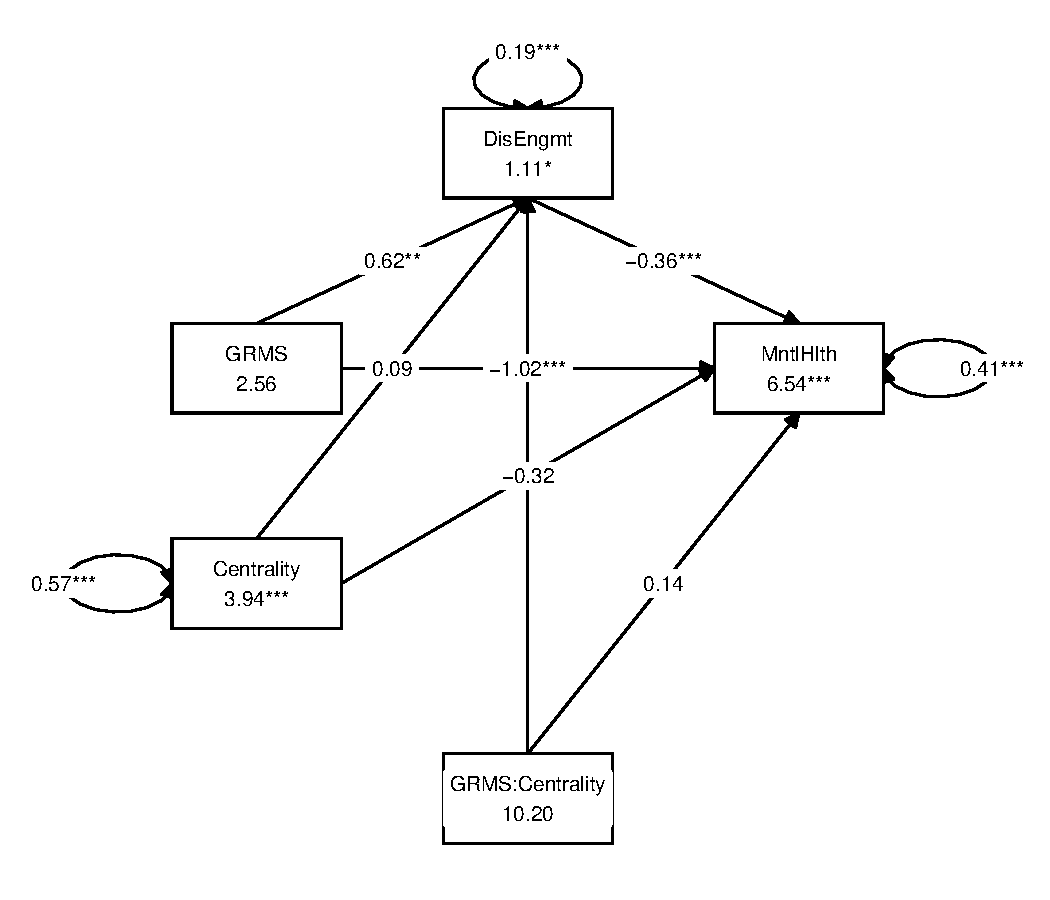
\includegraphics{05-SimpleMed_files/figure-latex/unnamed-chunk-28-1.pdf}

\begin{Shaded}
\begin{Highlighting}[]
\NormalTok{tidySEM}\SpecialCharTok{::}\FunctionTok{get\_layout}\NormalTok{(Kim\_fit\_covs)}
\end{Highlighting}
\end{Shaded}

\begin{verbatim}
##      [,1]  [,2]   [,3] 
## [1,] NA    "REMS" NA   
## [2,] "CMI" "ANX"  "PWB"
## attr(,"class")
## [1] "layout_matrix" "matrix"        "array"
\end{verbatim}

We can write code to remap them

\begin{Shaded}
\begin{Highlighting}[]
\NormalTok{med\_map3 }\OtherTok{\textless{}{-}}\NormalTok{ tidySEM}\SpecialCharTok{::}\FunctionTok{get\_layout}\NormalTok{(}
                                \StringTok{"ANX"}\NormalTok{, }\StringTok{""}\NormalTok{,   }\StringTok{"CMI"}\NormalTok{,  }\StringTok{""}\NormalTok{,}
                               \StringTok{"REMS"}\NormalTok{, }\StringTok{""}\NormalTok{,  }\StringTok{""}\NormalTok{,    }\StringTok{"PWB"}\NormalTok{, }\AttributeTok{rows=}\DecValTok{2}\NormalTok{)}
\NormalTok{med\_map3}
\end{Highlighting}
\end{Shaded}

\begin{verbatim}
##      [,1]   [,2] [,3]  [,4] 
## [1,] "ANX"  ""   "CMI" ""   
## [2,] "REMS" ""   ""    "PWB"
## attr(,"class")
## [1] "layout_matrix" "matrix"        "array"
\end{verbatim}

We run again with our map and BOOM! Still needs tinkering for gorgeous, but hey!

\begin{Shaded}
\begin{Highlighting}[]
\NormalTok{tidySEM}\SpecialCharTok{::}\FunctionTok{graph\_sem}\NormalTok{(Kim\_fit\_covs, }\AttributeTok{layout =}\NormalTok{ med\_map3, }\AttributeTok{rect\_width =} \FloatTok{1.5}\NormalTok{, }\AttributeTok{rect\_height =} \FloatTok{1.25}\NormalTok{,}
    \AttributeTok{spacing\_x =} \DecValTok{2}\NormalTok{, }\AttributeTok{spacing\_y =} \DecValTok{3}\NormalTok{, }\AttributeTok{text\_size =} \FloatTok{4.5}\NormalTok{)}
\end{Highlighting}
\end{Shaded}

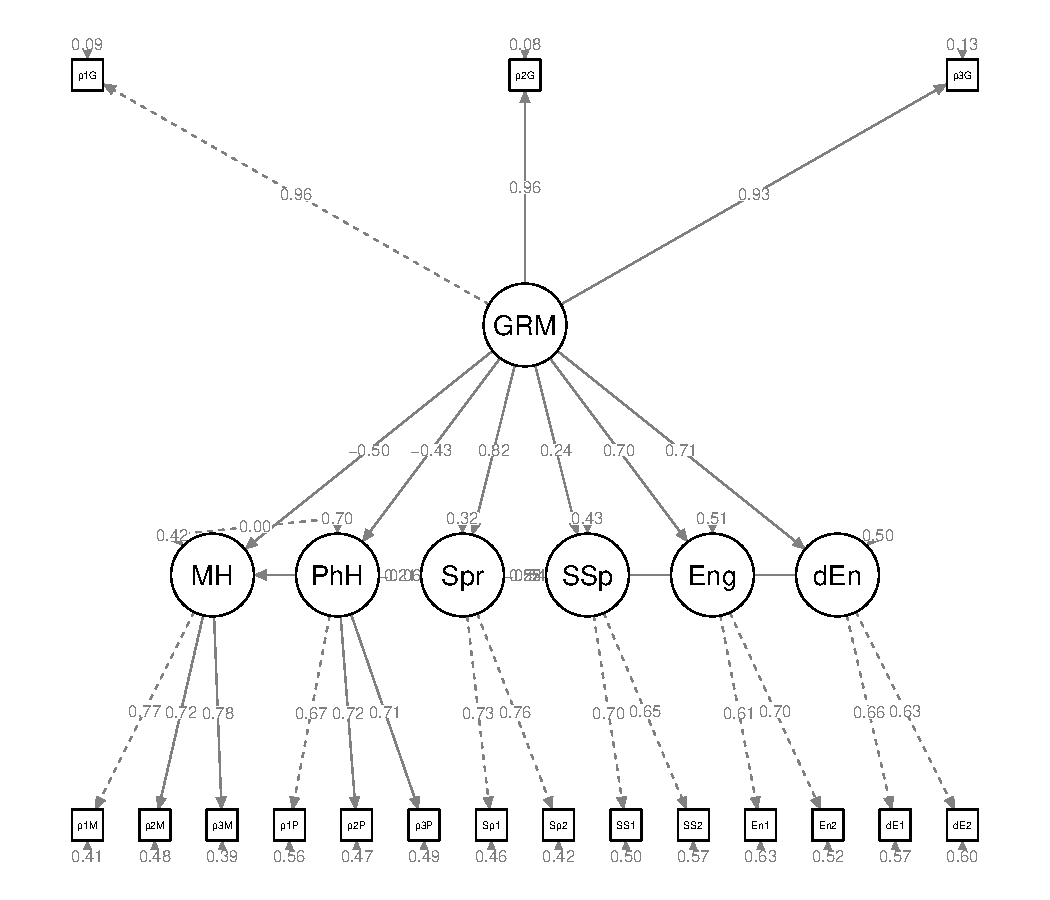
\includegraphics{05-SimpleMed_files/figure-latex/unnamed-chunk-31-1.pdf}

Below is code to create an outfile that could help with creating a table in a word document or spreadsheet. There will be output that is produced with SEM models that won't be relevant for this project.

\begin{Shaded}
\begin{Highlighting}[]
\FunctionTok{write.csv}\NormalTok{(Kcov\_ParEsts, }\AttributeTok{file =} \StringTok{"KimMedCov.csv"}\NormalTok{)}
\end{Highlighting}
\end{Shaded}

Table 3

\begin{longtable}[]{@{}
  >{\raggedright\arraybackslash}p{(\columnwidth - 0\tabcolsep) * \real{1.0000}}@{}}
\toprule\noalign{}
\begin{minipage}[b]{\linewidth}\raggedright
Model Coefficients Assessing Cultural Mistrust as a Mediator Between Racial Microaggressions and Well-Being
\end{minipage} \\
\midrule\noalign{}
\endhead
\bottomrule\noalign{}
\endlastfoot
\end{longtable}

\begin{longtable}[]{@{}
  >{\raggedright\arraybackslash}p{(\columnwidth - 6\tabcolsep) * \real{0.3012}}
  >{\centering\arraybackslash}p{(\columnwidth - 6\tabcolsep) * \real{0.3133}}
  >{\centering\arraybackslash}p{(\columnwidth - 6\tabcolsep) * \real{0.0843}}
  >{\centering\arraybackslash}p{(\columnwidth - 6\tabcolsep) * \real{0.3012}}@{}}
\toprule\noalign{}
\endhead
\bottomrule\noalign{}
\endlastfoot
& Cultural Mistrust (M) & & Well-Being (Y) \\
\end{longtable}

\begin{longtable}[]{@{}
  >{\raggedright\arraybackslash}p{(\columnwidth - 16\tabcolsep) * \real{0.2179}}
  >{\centering\arraybackslash}p{(\columnwidth - 16\tabcolsep) * \real{0.0897}}
  >{\centering\arraybackslash}p{(\columnwidth - 16\tabcolsep) * \real{0.1026}}
  >{\centering\arraybackslash}p{(\columnwidth - 16\tabcolsep) * \real{0.1026}}
  >{\centering\arraybackslash}p{(\columnwidth - 16\tabcolsep) * \real{0.1026}}
  >{\centering\arraybackslash}p{(\columnwidth - 16\tabcolsep) * \real{0.0897}}
  >{\centering\arraybackslash}p{(\columnwidth - 16\tabcolsep) * \real{0.1026}}
  >{\centering\arraybackslash}p{(\columnwidth - 16\tabcolsep) * \real{0.0897}}
  >{\centering\arraybackslash}p{(\columnwidth - 16\tabcolsep) * \real{0.1026}}@{}}
\toprule\noalign{}
\endhead
\bottomrule\noalign{}
\endlastfoot
Antecedent & path & \(B\) & \(SE\) & \(p\) & path & \(B\) & \(SE\) & \(p\) \\
constant & \(i_{M}\) & 2.697 & 0.245 & \textless0.001 & \(i_{Y}\) & 4.521 & 0.209 & \textless0.001 \\
REMS (X) & \(a\) & 1.349 & 0.191 & \textless0.001 & \(c'\) & -0.219 & 0.149 & 0.140 \\
CMI (M) & & & & & \(b\) & -0.163 & 0.051 & 0.001 \\
ANX (Cov) & & 0.198 & 0.096 & 0.039 & & -0.238 & 0.061 & \textless0.001 \\
\end{longtable}

\begin{longtable}[]{@{}
  >{\raggedright\arraybackslash}p{(\columnwidth - 6\tabcolsep) * \real{0.3012}}
  >{\centering\arraybackslash}p{(\columnwidth - 6\tabcolsep) * \real{0.3133}}
  >{\centering\arraybackslash}p{(\columnwidth - 6\tabcolsep) * \real{0.0843}}
  >{\centering\arraybackslash}p{(\columnwidth - 6\tabcolsep) * \real{0.3012}}@{}}
\toprule\noalign{}
\endhead
\bottomrule\noalign{}
\endlastfoot
& \(R^2\) = 36\% & & \(R^2\) = 35\% \\
\end{longtable}

\begin{longtable}[]{@{}
  >{\raggedright\arraybackslash}p{(\columnwidth - 0\tabcolsep) * \real{1.0000}}@{}}
\toprule\noalign{}
\endhead
\bottomrule\noalign{}
\endlastfoot
\emph{Note}. The value of the indirect effect was \(B = -.220, SE = 0.076, p = 0.004, 95CI(-0.385,-0.085)\). \\
\end{longtable}

\hypertarget{apa-style-write-up}{%
\subsection{APA Style Write-up}\label{apa-style-write-up}}

There are varying models for reporting the results of mediation. The Kim et al. \citep{kim_racial_2017} writeup is a great example. Rather than copying it directly, I have modeled my table after the ones in Hayes \citeyearpar{hayes_introduction_2018} text. You'll notice that information in the table and text are minimally overlapping. APA style cautions us against redundancy in text and table.

\textbf{Results}

A simple mediation model examined the degree to which cultural mistrust mediated the effect of racial microaggressions on psychological well-being. Using the \emph{lavaan} package (v 0.6-16) in R, coefficients for the each path, the indirect effect, and total effects were calculated. Additionally, the effect of covariate, anxiety, was mapped onto both the mediator and dependent variable. The model accounted for 36\% of the variance in cultural mistrust and 35\% of the variance in well-being. Supporting the notion of a mediated model, there was a statistically significant indirect effect \((B = -.220, SE = 0.076, p = 0.004, 95CI[-0.385,-0.085])\) in combination with a non-significant direct effect \((B = -0.219, p = 0.140)\) and a statistically significant total effect\((B = -0.440, p < 0.001)\).

\hypertarget{stay-tuned}{%
\section{STAY TUNED}\label{stay-tuned}}

A section on power analysis is planned and coming soon! My apologies that it's not quite \emph{R}eady.

\hypertarget{residual-and-related-questions}{%
\section{Residual and Related Questions\ldots{}}\label{residual-and-related-questions}}

..that you might have; or at least I had, but if had answered them earlier it would have disrupt the flow.

\begin{enumerate}
\def\labelenumi{\arabic{enumi}.}
\tightlist
\item
  Are you sure you can claim a significant indirect effect in the presence of a non-significant total effect? Hayes \citeyearpar{hayes_introduction_2018} is.

  \begin{itemize}
  \tightlist
  \item
    In the section subtitled, ``What about Baron \& Kenny'' (chapter 4), Hayes argues from both logical/philosophical and statistical perspectives that the size of the total effect does not constrain or determine the size of the indirect effect. That is, an indirect effect can be different from zero even when the total effect is not (pp.~117-119).\\
  \end{itemize}
\item
  The output we get is different from the output in the journal article being used as the research vignette. Why? And should we worry about it?

  \begin{itemize}
  \tightlist
  \item
    We are simulating data. This gives us some advantages in that (unless we specify it), we never have missingness and our variables should be normally distributed. Because we are working from means, standard deviations, and correlations, our data will never be the same as the original researcher. That said, we can compare our results to the journal to \emph{check out work.} In fact, in this very chapter, I got turned around (e.g., first accidentally swapping the mediator and IV; then using the wrong DV) and was able to compare my work against the journal article to correct my errors.
  \end{itemize}
\item
  Some of the statistics you are reporting are different than the ones in Hayes and the ones that use the PROCESS macro (e.g., what happened to the \emph{F} test)?

  \begin{itemize}
  \tightlist
  \item
    The default estimator for \emph{lavaan} is maximum likelihood (ML) and Hayes uses ordinary least squares (OLS). This affects both the values of coefficients, standard errors, AND the type of statistics that are reported.
  \item
    You can ask for OLS regression by adding the statement ``estimator =''GLS''. Even with this option, I have not discovered a way to obtain the \emph{F} tests for the overall model. Researchers seem to be comfortable with this, even asking for less than we did (e.g., many do not request R square).
  \item
    Best I can tell, researchers who do want this might use a combination of packages, using GLS estimators in \emph{lavaan} (this easily gets them the bootstrapped CIs) and the move to a different regression package to get the intercepts and \emph{F} tests. If I did this I would triple check to make sure that all the output really lined up.
  \end{itemize}
\item
  Why did we ignore the traditional fit statistics associated with structural equation modeling (e.g., CFI, RMSEA).

  \begin{itemize}
  \tightlist
  \item
    I hesitate to do this with models that do not include latent variables. Therefore, we asked for an ``in-between'' amount of info that should be sufficient for publication submission (any editor may have their own preferences and ask for more).
  \end{itemize}
\item
  What if I have missing data?

  \begin{itemize}
  \tightlist
  \item
    When we enter the \emph{lavaan} world we do get options other than multiple imputation. In today's example we used the ``sem'' fitting function. Unless otherwise specified, listwise deletion (deleting the entire case when one of its variables is used to estimate the model) is the default in \emph{lavaan}. If data are MCAR or MAR, you can add the argument \emph{missing = ``ml''} (or its alias \emph{missing = ``fiml''}). More here \url{https://users.ugent.be/~yrosseel/lavaan/lavaan2.pdf} on the 1.7/Missing data in lavaan slide.
  \item
    That said, the type of estimator matters. If you estimate your data with GLS (generalized least squares) or WLS (weighted least squares), you are required to have complete data (however you got it). We used maximum likelihood and, even though we had non-missing data, I used the \emph{missing = ``fiml''} code.
  \end{itemize}
\end{enumerate}

\hypertarget{practice-problems-4}{%
\section{Practice Problems}\label{practice-problems-4}}

The three problems described below are designed to grow with the subsequent chapters on complex mediation and conditional process analysis (i.e,. moderated mediation). Therefore, I recommend that you select a dataset that includes at least four variables. If you are new to this topic, you may wish to select variables that are all continuously scaled. The IV and moderator (subsequent chapters) could be categorical (if they are dichotomous, please use 0/1 coding; if they have more than one category it is best if they are ordered). You will likely encounter challenges that were not covered in this chapter. Search for and try out solutions, knowing that there are multiple paths through the analysis.

The suggested practice problem for this chapter is to conduct a simple mediation.

\hypertarget{problem-1-rework-the-research-vignette-as-demonstrated-but-change-the-random-seed}{%
\subsection{Problem \#1: Rework the research vignette as demonstrated, but change the random seed}\label{problem-1-rework-the-research-vignette-as-demonstrated-but-change-the-random-seed}}

If this topic feels a bit overwhelming, simply change the random seed in the data simulation, then rework the problem. This should provide minor changes to the data (maybe in the second or third decimal point), but the results will likely be very similar.

\hypertarget{problem-2-rework-the-research-vignette-but-swap-one-or-more-variables}{%
\subsection{Problem \#2: Rework the research vignette, but swap one or more variables}\label{problem-2-rework-the-research-vignette-but-swap-one-or-more-variables}}

Use the simulated data, but select one of the other models that was evaluated in the Kim et al. \citeyearpar{kim_racial_2017} study. Compare your results to those reported in the mansucript.

\hypertarget{problem-3-use-other-data-that-is-available-to-you}{%
\subsection{Problem \#3: Use other data that is available to you}\label{problem-3-use-other-data-that-is-available-to-you}}

Using data for which you have permission and access (e.g., IRB approved data you have collected or from your lab; data you simulate from a published article; data from an open science repository; data from other chapters in this OER), complete a simple mediation.

\hypertarget{grading-rubric-4}{%
\subsection{Grading Rubric}\label{grading-rubric-4}}

\begin{longtable}[]{@{}
  >{\raggedright\arraybackslash}p{(\columnwidth - 4\tabcolsep) * \real{0.7642}}
  >{\centering\arraybackslash}p{(\columnwidth - 4\tabcolsep) * \real{0.1220}}
  >{\centering\arraybackslash}p{(\columnwidth - 4\tabcolsep) * \real{0.1138}}@{}}
\toprule\noalign{}
\begin{minipage}[b]{\linewidth}\raggedright
Assignment Component
\end{minipage} & \begin{minipage}[b]{\linewidth}\centering
Points Possible
\end{minipage} & \begin{minipage}[b]{\linewidth}\centering
Points Earned
\end{minipage} \\
\midrule\noalign{}
\endhead
\bottomrule\noalign{}
\endlastfoot
1. Assign each variable to the X, Y, or M roles (ok but not required to include a cov) & 5 & \_\_\_\_\_ \\
2. Import the data and format the variables in the model & 5 & \_\_\_\_\_ \\
3. Specify and run the lavaan model & 5 & \_\_\_\_\_ \\
4. Use tidySEM to create a figure that represents your results & 5 & \_\_\_\_\_ \\
5. Create a table that includes regression output for the M and Y variables & 5 & \_\_\_\_\_ \\
6. Represent your work in an APA-style write-up & 5 & \_\_\_\_\_ \\
7. Explanation to grader & 5 & \_\_\_\_\_ \\
8. Be able to hand-calculate the indirect, direct, and total effects from the a, b, \& c' paths & 5 & \_\_\_\_\_ \\
\textbf{Totals} & 35 & \_\_\_\_\_ \\
\end{longtable}

\hypertarget{homeworked-example-2}{%
\section{Homeworked Example}\label{homeworked-example-2}}

\href{https://youtu.be/hXTFPSQrjpQ}{Screencast Link}

For more information about the data used in this homeworked example, please refer to the description and codebook located at the end of the \href{https://lhbikos.github.io/ReCenterPsychStats/ReCintro.html\#introduction-to-the-data-set-used-for-homeworked-examples}{introductory lesson} in \href{https://lhbikos.github.io/ReCenterPsychStats/}{ReCentering Psych Stats}. An .rds file which holds the data is located in the \href{https://github.com/lhbikos/ReC_MultivModel/tree/main/Worked_Examples}{Worked Examples} folder at the GitHub site the hosts the OER. The file name is \emph{ReC.rds}.

The suggested practice problem for this chapter is to conduct a simple mediation.

\hypertarget{assign-each-variable-to-the-x-y-or-m-roles-ok-but-not-required-to-include-a-covariate}{%
\subsection{Assign each variable to the X, Y, or M roles (ok but not required to include a covariate)}\label{assign-each-variable-to-the-x-y-or-m-roles-ok-but-not-required-to-include-a-covariate}}

X = Centering: explicit recentering (0 = precentered; 1 = recentered) M = TradPed: traditional pedagogy (continuously scaled with higher scores being more favorable) Y = SRPed: socially responsive pedagogy (continuously scaled with higher scores being more favorable)

\hypertarget{specify-a-research-model-2}{%
\subsection*{Specify a research model}\label{specify-a-research-model-2}}


I am hypothesizing that the evaluation of social responsive pedagogy is predicted by intentional recentering through traditional pedagogy.

\hypertarget{import-the-data-and-format-the-variables-in-the-model}{%
\subsection*{Import the data and format the variables in the model}\label{import-the-data-and-format-the-variables-in-the-model}}


\begin{Shaded}
\begin{Highlighting}[]
\NormalTok{raw }\OtherTok{\textless{}{-}} \FunctionTok{readRDS}\NormalTok{(}\StringTok{"ReC.rds"}\NormalTok{)}
\end{Highlighting}
\end{Shaded}

I need to score the TradPed and SRPed variables

\begin{Shaded}
\begin{Highlighting}[]
\NormalTok{TradPed\_vars }\OtherTok{\textless{}{-}} \FunctionTok{c}\NormalTok{(}\StringTok{"ClearResponsibilities"}\NormalTok{, }\StringTok{"EffectiveAnswers"}\NormalTok{, }\StringTok{"Feedback"}\NormalTok{,}
    \StringTok{"ClearOrganization"}\NormalTok{, }\StringTok{"ClearPresentation"}\NormalTok{)}
\NormalTok{raw}\SpecialCharTok{$}\NormalTok{TradPed }\OtherTok{\textless{}{-}}\NormalTok{ sjstats}\SpecialCharTok{::}\FunctionTok{mean\_n}\NormalTok{(raw[, ..TradPed\_vars], }\FloatTok{0.75}\NormalTok{)}

\NormalTok{SRPed\_vars }\OtherTok{\textless{}{-}} \FunctionTok{c}\NormalTok{(}\StringTok{"InclusvClassrm"}\NormalTok{, }\StringTok{"EquitableEval"}\NormalTok{, }\StringTok{"MultPerspectives"}\NormalTok{,}
    \StringTok{"DEIintegration"}\NormalTok{)}
\NormalTok{raw}\SpecialCharTok{$}\NormalTok{SRPed }\OtherTok{\textless{}{-}}\NormalTok{ sjstats}\SpecialCharTok{::}\FunctionTok{mean\_n}\NormalTok{(raw[, ..SRPed\_vars], }\FloatTok{0.75}\NormalTok{)}
\end{Highlighting}
\end{Shaded}

I will create a babydf.

\begin{Shaded}
\begin{Highlighting}[]
\NormalTok{babydf }\OtherTok{\textless{}{-}}\NormalTok{ dplyr}\SpecialCharTok{::}\FunctionTok{select}\NormalTok{(raw, Centering, TradPed, SRPed)}
\end{Highlighting}
\end{Shaded}

Let's check the structure of the variables:

\begin{verbatim}
str(babydf)
\end{verbatim}

\hypertarget{specify-and-run-the-lavaan-model}{%
\subsection*{Specify and run the lavaan model}\label{specify-and-run-the-lavaan-model}}


\begin{Shaded}
\begin{Highlighting}[]
\NormalTok{ReCMed }\OtherTok{\textless{}{-}} \StringTok{"}
\StringTok{          SRPed \textasciitilde{} b*TradPed + c\_p*Centering}
\StringTok{          TradPed \textasciitilde{} a*Centering}
\StringTok{          }
\StringTok{          indirect :=  a*b}
\StringTok{          direct  := c\_p}
\StringTok{          total\_c  := c\_p + (a*b)}
\StringTok{          "}

\FunctionTok{set.seed}\NormalTok{(}\DecValTok{231002}\NormalTok{)  }\CommentTok{\#needed for reproducible results since lavaan introduced randomness into some procedures}
\NormalTok{ReCfit }\OtherTok{\textless{}{-}}\NormalTok{ lavaan}\SpecialCharTok{::}\FunctionTok{sem}\NormalTok{(ReCMed, }\AttributeTok{data =}\NormalTok{ babydf, }\AttributeTok{se =} \StringTok{"bootstrap"}\NormalTok{, }\AttributeTok{missing =} \StringTok{"fiml"}\NormalTok{)}
\NormalTok{ReCsummary }\OtherTok{\textless{}{-}}\NormalTok{ lavaan}\SpecialCharTok{::}\FunctionTok{summary}\NormalTok{(ReCfit, }\AttributeTok{standardized =}\NormalTok{ T, }\AttributeTok{rsq =}\NormalTok{ T, }\AttributeTok{fit =} \ConstantTok{TRUE}\NormalTok{,}
    \AttributeTok{ci =} \ConstantTok{TRUE}\NormalTok{)}
\NormalTok{ReC\_ParamEsts }\OtherTok{\textless{}{-}}\NormalTok{ lavaan}\SpecialCharTok{::}\FunctionTok{parameterEstimates}\NormalTok{(ReCfit, }\AttributeTok{boot.ci.type =} \StringTok{"bca.simple"}\NormalTok{,}
    \AttributeTok{standardized =} \ConstantTok{TRUE}\NormalTok{)}
\NormalTok{ReCsummary}
\end{Highlighting}
\end{Shaded}

\begin{verbatim}
## lavaan 0.6.16 ended normally after 14 iterations
## 
##   Estimator                                         ML
##   Optimization method                           NLMINB
##   Number of model parameters                         7
## 
##   Number of observations                           310
##   Number of missing patterns                         4
## 
## Model Test User Model:
##                                                       
##   Test statistic                                 0.000
##   Degrees of freedom                                 0
## 
## Model Test Baseline Model:
## 
##   Test statistic                               216.492
##   Degrees of freedom                                 3
##   P-value                                        0.000
## 
## User Model versus Baseline Model:
## 
##   Comparative Fit Index (CFI)                    1.000
##   Tucker-Lewis Index (TLI)                       1.000
##                                                       
##   Robust Comparative Fit Index (CFI)             1.000
##   Robust Tucker-Lewis Index (TLI)                1.000
## 
## Loglikelihood and Information Criteria:
## 
##   Loglikelihood user model (H0)               -506.434
##   Loglikelihood unrestricted model (H1)       -506.434
##                                                       
##   Akaike (AIC)                                1026.868
##   Bayesian (BIC)                              1053.024
##   Sample-size adjusted Bayesian (SABIC)       1030.823
## 
## Root Mean Square Error of Approximation:
## 
##   RMSEA                                          0.000
##   90 Percent confidence interval - lower         0.000
##   90 Percent confidence interval - upper         0.000
##   P-value H_0: RMSEA <= 0.050                       NA
##   P-value H_0: RMSEA >= 0.080                       NA
##                                                       
##   Robust RMSEA                                   0.000
##   90 Percent confidence interval - lower         0.000
##   90 Percent confidence interval - upper         0.000
##   P-value H_0: Robust RMSEA <= 0.050                NA
##   P-value H_0: Robust RMSEA >= 0.080                NA
## 
## Standardized Root Mean Square Residual:
## 
##   SRMR                                           0.000
## 
## Parameter Estimates:
## 
##   Standard errors                            Bootstrap
##   Number of requested bootstrap draws             1000
##   Number of successful bootstrap draws            1000
## 
## Regressions:
##                    Estimate  Std.Err  z-value  P(>|z|) ci.lower ci.upper
##   SRPed ~                                                               
##     TradPed    (b)    0.549    0.046   12.067    0.000    0.458    0.645
##     Centerng (c_p)    0.127    0.047    2.684    0.007    0.036    0.219
##   TradPed ~                                                             
##     Centerng   (a)   -0.101    0.090   -1.121    0.262   -0.287    0.080
##    Std.lv  Std.all
##                   
##     0.549    0.716
##     0.127    0.107
##                   
##    -0.101   -0.066
## 
## Intercepts:
##                    Estimate  Std.Err  z-value  P(>|z|) ci.lower ci.upper
##    .SRPed             2.006    0.231    8.689    0.000    1.543    2.442
##    .TradPed           4.394    0.139   31.707    0.000    4.109    4.675
##    Std.lv  Std.all
##     2.006    3.440
##     4.394    5.778
## 
## Variances:
##                    Estimate  Std.Err  z-value  P(>|z|) ci.lower ci.upper
##    .SRPed             0.165    0.017    9.467    0.000    0.130    0.203
##    .TradPed           0.576    0.070    8.225    0.000    0.444    0.724
##    Std.lv  Std.all
##     0.165    0.486
##     0.576    0.996
## 
## R-Square:
##                    Estimate
##     SRPed             0.514
##     TradPed           0.004
## 
## Defined Parameters:
##                    Estimate  Std.Err  z-value  P(>|z|) ci.lower ci.upper
##     indirect         -0.056    0.052   -1.077    0.282   -0.168    0.042
##     direct            0.127    0.047    2.682    0.007    0.036    0.219
##     total_c           0.071    0.068    1.045    0.296   -0.055    0.204
##    Std.lv  Std.all
##    -0.056   -0.047
##     0.127    0.107
##     0.071    0.060
\end{verbatim}

\begin{Shaded}
\begin{Highlighting}[]
\NormalTok{ReC\_ParamEsts}
\end{Highlighting}
\end{Shaded}

\begin{verbatim}
##          lhs op       rhs    label    est    se      z pvalue ci.lower ci.upper
## 1      SRPed  ~   TradPed        b  0.549 0.046 12.067  0.000    0.459    0.645
## 2      SRPed  ~ Centering      c_p  0.127 0.047  2.684  0.007    0.032    0.211
## 3    TradPed  ~ Centering        a -0.101 0.090 -1.121  0.262   -0.292    0.075
## 4      SRPed ~~     SRPed           0.165 0.017  9.467  0.000    0.135    0.209
## 5    TradPed ~~   TradPed           0.576 0.070  8.225  0.000    0.462    0.741
## 6  Centering ~~ Centering           0.241 0.000     NA     NA    0.241    0.241
## 7      SRPed ~1                     2.006 0.231  8.689  0.000    1.534    2.433
## 8    TradPed ~1                     4.394 0.139 31.707  0.000    4.114    4.683
## 9  Centering ~1                     1.406 0.000     NA     NA    1.406    1.406
## 10  indirect :=       a*b indirect -0.056 0.052 -1.077  0.282   -0.171    0.038
## 11    direct :=       c_p   direct  0.127 0.047  2.682  0.007    0.032    0.211
## 12   total_c := c_p+(a*b)  total_c  0.071 0.068  1.045  0.296   -0.053    0.205
##    std.lv std.all std.nox
## 1   0.549   0.716   0.716
## 2   0.127   0.107   0.217
## 3  -0.101  -0.066  -0.133
## 4   0.165   0.486   0.486
## 5   0.576   0.996   0.996
## 6   0.241   1.000   0.241
## 7   2.006   3.440   3.440
## 8   4.394   5.778   5.778
## 9   1.406   2.863   1.406
## 10 -0.056  -0.047  -0.096
## 11  0.127   0.107   0.217
## 12  0.071   0.060   0.122
\end{verbatim}

\hypertarget{use-tidysem-to-create-a-figure-that-represents-your-results}{%
\subsection*{Use tidySEM to create a figure that represents your results}\label{use-tidysem-to-create-a-figure-that-represents-your-results}}


\begin{Shaded}
\begin{Highlighting}[]
\CommentTok{\# only worked when I used the library to turn on all these pkgs}
\FunctionTok{library}\NormalTok{(lavaan)}
\FunctionTok{library}\NormalTok{(dplyr)}
\FunctionTok{library}\NormalTok{(ggplot2)}
\FunctionTok{library}\NormalTok{(tidySEM)}
\NormalTok{tidySEM}\SpecialCharTok{::}\FunctionTok{graph\_sem}\NormalTok{(}\AttributeTok{model =}\NormalTok{ ReCfit)}
\end{Highlighting}
\end{Shaded}

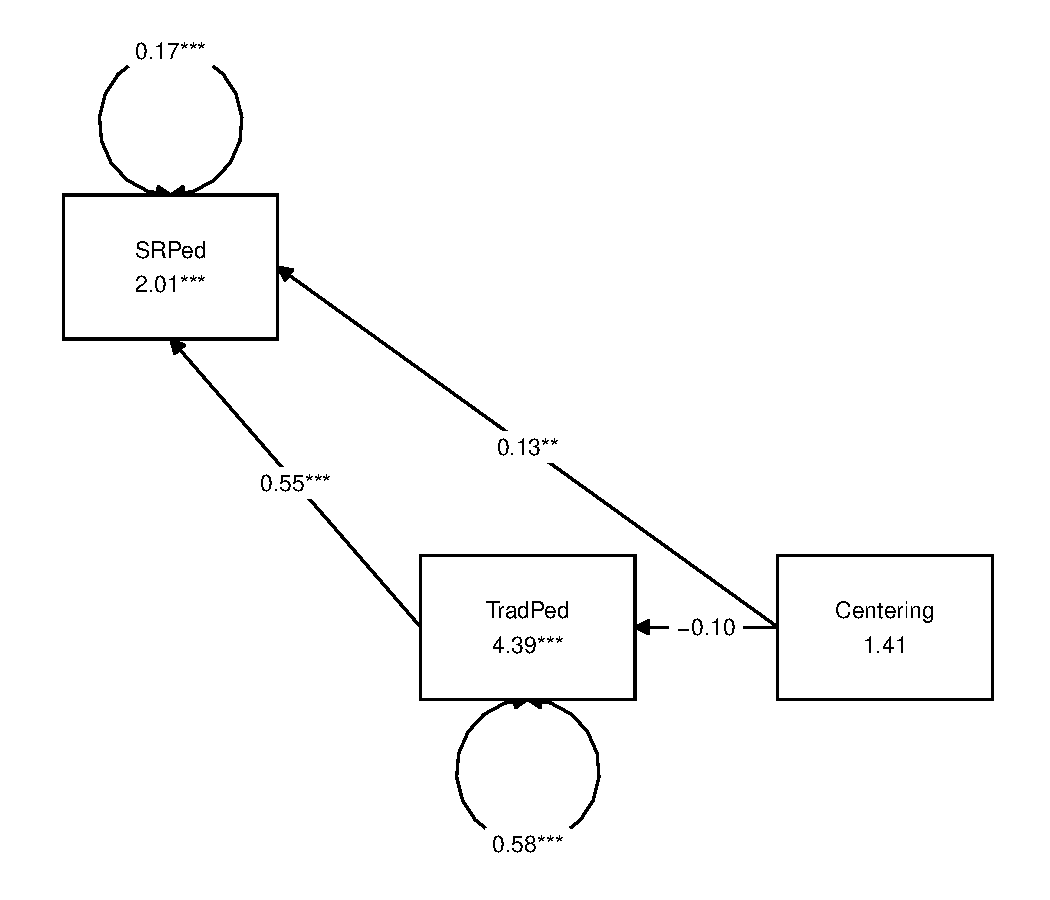
\includegraphics{05-SimpleMed_files/figure-latex/unnamed-chunk-40-1.pdf}

\begin{Shaded}
\begin{Highlighting}[]
\NormalTok{tidySEM}\SpecialCharTok{::}\FunctionTok{get\_layout}\NormalTok{(ReCfit)}
\end{Highlighting}
\end{Shaded}

\begin{verbatim}
##      [,1]    [,2]      [,3]       
## [1,] "SRPed" "TradPed" "Centering"
## attr(,"class")
## [1] "layout_matrix" "matrix"        "array"
\end{verbatim}

We can write code to remap them

\begin{Shaded}
\begin{Highlighting}[]
\NormalTok{med\_map }\OtherTok{\textless{}{-}}\NormalTok{ tidySEM}\SpecialCharTok{::}\FunctionTok{get\_layout}\NormalTok{(}\StringTok{""}\NormalTok{, }\StringTok{"TradPed"}\NormalTok{, }\StringTok{""}\NormalTok{, }\StringTok{"Centering"}\NormalTok{, }\StringTok{""}\NormalTok{, }\StringTok{"SRPed"}\NormalTok{,}
    \AttributeTok{rows =} \DecValTok{2}\NormalTok{)}
\NormalTok{med\_map}
\end{Highlighting}
\end{Shaded}

\begin{verbatim}
##      [,1]        [,2]      [,3]   
## [1,] ""          "TradPed" ""     
## [2,] "Centering" ""        "SRPed"
## attr(,"class")
## [1] "layout_matrix" "matrix"        "array"
\end{verbatim}

\begin{Shaded}
\begin{Highlighting}[]
\NormalTok{tidySEM}\SpecialCharTok{::}\FunctionTok{graph\_sem}\NormalTok{(ReCfit, }\AttributeTok{layout=}\NormalTok{med\_map,  }\AttributeTok{rect\_width =} \FloatTok{1.5}\NormalTok{, }\AttributeTok{rect\_height =} \FloatTok{1.25}\NormalTok{, }\AttributeTok{spacing\_x =} \DecValTok{2}\NormalTok{, }\AttributeTok{spacing\_y =} \DecValTok{3}\NormalTok{, }\AttributeTok{text\_size =} \FloatTok{4.5}\NormalTok{)}
\end{Highlighting}
\end{Shaded}

\includegraphics{05-SimpleMed_files/figure-latex/unnamed-chunk-43-1.pdf}

\hypertarget{create-a-table-that-includes-regression-output-for-the-m-and-y-variables}{%
\subsection*{Create a table that includes regression output for the M and Y variables}\label{create-a-table-that-includes-regression-output-for-the-m-and-y-variables}}


\begin{Shaded}
\begin{Highlighting}[]
\FunctionTok{write.csv}\NormalTok{(ReC\_ParamEsts, }\AttributeTok{file =} \StringTok{"ReCSimpMed.csv"}\NormalTok{)}
\end{Highlighting}
\end{Shaded}

Table 1

\begin{longtable}[]{@{}
  >{\raggedright\arraybackslash}p{(\columnwidth - 0\tabcolsep) * \real{1.0000}}@{}}
\toprule\noalign{}
\begin{minipage}[b]{\linewidth}\raggedright
Model Coefficients Assessing Traditional Pedagogy as a Mediator Between Centering and Socially Responsive Pedagogy
\end{minipage} \\
\midrule\noalign{}
\endhead
\bottomrule\noalign{}
\endlastfoot
\end{longtable}

\begin{longtable}[]{@{}
  >{\raggedright\arraybackslash}p{(\columnwidth - 4\tabcolsep) * \real{0.1889}}
  >{\centering\arraybackslash}p{(\columnwidth - 4\tabcolsep) * \real{0.4000}}
  >{\centering\arraybackslash}p{(\columnwidth - 4\tabcolsep) * \real{0.4111}}@{}}
\toprule\noalign{}
\endhead
\bottomrule\noalign{}
\endlastfoot
& Traditional Pedagogy (M) & Socially Responsive Pedagogy (Y) \\
\end{longtable}

\begin{longtable}[]{@{}
  >{\raggedright\arraybackslash}p{(\columnwidth - 16\tabcolsep) * \real{0.2024}}
  >{\centering\arraybackslash}p{(\columnwidth - 16\tabcolsep) * \real{0.0833}}
  >{\centering\arraybackslash}p{(\columnwidth - 16\tabcolsep) * \real{0.1071}}
  >{\centering\arraybackslash}p{(\columnwidth - 16\tabcolsep) * \real{0.0952}}
  >{\centering\arraybackslash}p{(\columnwidth - 16\tabcolsep) * \real{0.1071}}
  >{\centering\arraybackslash}p{(\columnwidth - 16\tabcolsep) * \real{0.0833}}
  >{\centering\arraybackslash}p{(\columnwidth - 16\tabcolsep) * \real{0.0952}}
  >{\centering\arraybackslash}p{(\columnwidth - 16\tabcolsep) * \real{0.0952}}
  >{\centering\arraybackslash}p{(\columnwidth - 16\tabcolsep) * \real{0.1310}}@{}}
\toprule\noalign{}
\endhead
\bottomrule\noalign{}
\endlastfoot
Antecedent & path & \(B\) & \(SE\) & \(p\) & path & \(B\) & \(SE\) & \(p\) \\
constant & \(i_{M}\) & 4.394 & 0.139 & \textless{} 0.001 & \(i_{Y}\) & 2.006 & 0.231 & \textless{} 0.001 \\
Centering (X) & \(a\) & -0.101 & 0.090 & 0.262 & \(c'\) & 0.127 & 0.047 & 0.007 \\
TradPed (M) & & & & & \(b\) & 0.549 & 0.046 & \textless{} 0.001 \\
\end{longtable}

\begin{longtable}[]{@{}
  >{\raggedright\arraybackslash}p{(\columnwidth - 6\tabcolsep) * \real{0.2809}}
  >{\centering\arraybackslash}p{(\columnwidth - 6\tabcolsep) * \real{0.3146}}
  >{\centering\arraybackslash}p{(\columnwidth - 6\tabcolsep) * \real{0.0787}}
  >{\centering\arraybackslash}p{(\columnwidth - 6\tabcolsep) * \real{0.3258}}@{}}
\toprule\noalign{}
\endhead
\bottomrule\noalign{}
\endlastfoot
& \(R^2\) = 0.4\% & & \(R^2\) = 51\% \\
\end{longtable}

\begin{longtable}[]{@{}
  >{\raggedright\arraybackslash}p{(\columnwidth - 0\tabcolsep) * \real{1.0000}}@{}}
\toprule\noalign{}
\endhead
\bottomrule\noalign{}
\endlastfoot
\emph{Note}. Centering: 0 = pre-centered, 1 = recentered. TradPed is traditional pedagogy. The value of the indirect effect was \(B = -0.056, SE = 0.051, p = 0.272, 95CI(-0.163,0.035)\) \\
\end{longtable}

\hypertarget{represent-your-work-in-an-apa-style-write-up}{%
\subsection*{Represent your work in an APA-style write-up}\label{represent-your-work-in-an-apa-style-write-up}}


A simple mediation model examined the degree to which evaluations of traditional pedagogy mediated the relation of explicit recentering on socially responsive pedagogy. Using the \emph{lavaan} package (v 0.6-16) in R, coefficients for each path, the indirect effect, and total effects were calculated. These values are presented in Table 1 and illustrated in Figure 1. Results suggested that neglibible (.4\%) of the variance was accounted for in traditional pedagogy. In contrast 51\% of the variance was accounted for in socially responsive pedagogy. The indirect effect \((B = -0.056, SE = 0.051, p = 0.272, 95CI[-0.163,0.035])\) was statistically significant. Comparing total and direct effects, the total effect of centering and traditional pedagogy on socially responsive pedagogy was not statistically significant \((B = 0.071, p = 0.302)\). In contrast, the direct effect was (\(B = 0.127, p = 0.008\) was not). This suggests that while centering and traditional pedagogy do influence socially responsive pedagogy, their influence is relatively independent.

\begin{Shaded}
\begin{Highlighting}[]
\NormalTok{apaTables}\SpecialCharTok{::}\FunctionTok{apa.cor.table}\NormalTok{(babydf, }\AttributeTok{table.number =} \DecValTok{1}\NormalTok{, }\AttributeTok{show.sig.stars =} \ConstantTok{TRUE}\NormalTok{,}
    \AttributeTok{landscape =} \ConstantTok{TRUE}\NormalTok{, }\AttributeTok{filename =} \ConstantTok{NA}\NormalTok{)}
\end{Highlighting}
\end{Shaded}

\begin{verbatim}
## 
## 
## Table 1 
## 
## Means, standard deviations, and correlations with confidence intervals
##  
## 
##   Variable   M    SD   1         
##   1. TradPed 4.25 0.76           
##                                  
##   2. SRPed   4.52 0.58 .71**     
##                        [.65, .76]
##                                  
## 
## Note. M and SD are used to represent mean and standard deviation, respectively.
## Values in square brackets indicate the 95% confidence interval.
## The confidence interval is a plausible range of population correlations 
## that could have caused the sample correlation (Cumming, 2014).
##  * indicates p < .05. ** indicates p < .01.
## 
\end{verbatim}

\hypertarget{explanation-to-grader}{%
\subsection*{Explanation to grader}\label{explanation-to-grader}}


\hypertarget{be-able-to-hand-calculate-the-indirect-direct-and-total-effects-from-the-a-b-c-paths}{%
\subsection*{Be able to hand-calculate the indirect, direct, and total effects from the a, b, \& c' paths}\label{be-able-to-hand-calculate-the-indirect-direct-and-total-effects-from-the-a-b-c-paths}}


\begin{itemize}
\tightlist
\item
  Indirect = a*b
\item
  Direct = Total minus indirect
\item
  Total = (a*b) + c'
\end{itemize}

\hypertarget{CompMed}{%
\chapter{Complex Mediation}\label{CompMed}}

\href{https://youtube.com/playlist?list=PLtz5cFLQl4KPxygMnwxro3FkuJj2rN6p-\&si=a7lIlFcLkMQzTc19}{Screencasted Lecture Link}

The focus of this chapter is the extension of simple mediation to models with multiple mediators. In these models with greater complexity we look at both parallel and serial mediation. There is also more elaboration on some of the conceptual issues related to the estimation of indirect effects.

\hypertarget{navigating-this-lesson-5}{%
\section{Navigating this Lesson}\label{navigating-this-lesson-5}}

There is about 1 hour and 20 minutes of lecture. If you work through the materials with me it would be plan for an additional two hours.

While the majority of R objects and data you will need are created within the R script that sources the chapter, there are a few that cannot be created from within the R framework. Additionally, sometimes links fail. All original materials are provided at the \href{https://https://github.com/lhbikos/ReC_MultivModel}{Github site} that hosts the book. More detailed guidelines for ways to access all these materials are provided in the OER's \href{https://lhbikos.github.io/ReCenterPsychStats/ReCintro.html\#introduction-to-the-data-set-used-for-homeworked-examples}{introduction}

\hypertarget{learning-objectives-5}{%
\subsection{Learning Objectives}\label{learning-objectives-5}}

Learning objectives from this lecture include the following:

\begin{itemize}
\tightlist
\item
  Define \emph{epiphenomality} and explain how it is related to (and supports the notion of) multiple mediation.
\item
  Distinguish between parallel and serial mediation models.
\item
  Locate and interpret \emph{lavaan} output from multiply mediated models including
\item
  identifying coefficients,
\item
  percentage of variance accounted for,\\
\item
  all the effects (total, direct, indirect, total indirect),
\item
  contrasts (comparing the significance of the indirect effects).
\item
  Explain the limitations of the classic approach \citep{baron_moderator-mediator_1986} to mediation.
\end{itemize}

\hypertarget{planning-for-practice-5}{%
\subsection{Planning for Practice}\label{planning-for-practice-5}}

The suggestions for practice in this chapter include conducting parallel, serial, and/or mediation models. Options of graded complexity could include:

\begin{itemize}
\tightlist
\item
  Rework the problem in the chapter by changing the random seed in the code that simulates the data. This should provide minor changes to the data, but the results will likely be very similar.
\item
  There are a number of variables in the dataset that sourced the research vignettes for this and the prior chapter on \protect\hyperlink{SimpleMed}{simple mediation}. Swap out one or more variables in a parallel or serial (or both) model.
\item
  Conduct a parallel or serial (or both) mediation with data to which you have access. This could include data you simulate on your own or from a published article.
\end{itemize}

\hypertarget{readings-resources-5}{%
\subsection{Readings \& Resources}\label{readings-resources-5}}

In preparing this chapter, I drew heavily from the following resource(s). Other resources are cited (when possible, linked) in the text with complete citations in the reference list.

\begin{itemize}
\tightlist
\item
  Hayes, A. F. (2022). \emph{Introduction to mediation, moderation, and conditional process analysis: A regression-based approach}. New York, NY: Guilford Press.

  \begin{itemize}
  \tightlist
  \item
    \textbf{Chapter 5: More than one mediator}: This chapter walks the reader through parallel and serial mediation models. We will do both!
  \item
    \textbf{Appendix A: Using PROCESS}: An essential tool for PROCESS users because, even when we are in the R environment, this is the ``idea book.'' That is, the place where all the path models are presented in figures.
  \end{itemize}
\end{itemize}

\hypertarget{packages-5}{%
\subsection{Packages}\label{packages-5}}

The script below will (a) check to see if the following packages are installed on your computer and, if not (b) install them.

\begin{Shaded}
\begin{Highlighting}[]
\CommentTok{\# will install the package if not already installed}
\ControlFlowTok{if}\NormalTok{ (}\SpecialCharTok{!}\FunctionTok{require}\NormalTok{(lavaan)) \{}
    \FunctionTok{install.packages}\NormalTok{(}\StringTok{"lavaan"}\NormalTok{)}
\NormalTok{\}}
\ControlFlowTok{if}\NormalTok{ (}\SpecialCharTok{!}\FunctionTok{require}\NormalTok{(tidyverse)) \{}
    \FunctionTok{install.packages}\NormalTok{(}\StringTok{"tidyverse"}\NormalTok{)}
\NormalTok{\}}
\ControlFlowTok{if}\NormalTok{ (}\SpecialCharTok{!}\FunctionTok{require}\NormalTok{(dplyr)) \{}
    \FunctionTok{install.packages}\NormalTok{(}\StringTok{"dplyr"}\NormalTok{)}
\NormalTok{\}}
\ControlFlowTok{if}\NormalTok{ (}\SpecialCharTok{!}\FunctionTok{require}\NormalTok{(psych)) \{}
    \FunctionTok{install.packages}\NormalTok{(}\StringTok{"psych"}\NormalTok{)}
\NormalTok{\}}
\ControlFlowTok{if}\NormalTok{ (}\SpecialCharTok{!}\FunctionTok{require}\NormalTok{(apaTables)) \{}
    \FunctionTok{install.packages}\NormalTok{(}\StringTok{"apaTables"}\NormalTok{)}
\NormalTok{\}}
\ControlFlowTok{if}\NormalTok{ (}\SpecialCharTok{!}\FunctionTok{require}\NormalTok{(tidySEM)) \{}
    \FunctionTok{install.packages}\NormalTok{(}\StringTok{"tidySEM"}\NormalTok{)}
\NormalTok{\}}
\end{Highlighting}
\end{Shaded}

\hypertarget{complex-mediation}{%
\section{Complex Mediation}\label{complex-mediation}}

The simple mediation model is quite popular, but also limiting in that it:

\begin{itemize}
\tightlist
\item
  frequently oversimplifies the processes we want to study, and
\item
  is likely mis-specified, in that there are unmodeled mechanisms.
\end{itemize}

Hayes \citeyearpar{hayes_more_2022} identified four reasons to consider multiply mediated models:

\begin{itemize}
\tightlist
\item
  We are generally interested in MULTIPLE mechanisms
\item
  A mechanism (such as a mediator) in the model, might, itself be mediated (i.e., mediated mediation)
\item
  \emph{Epiphenomenality} (``unknown confounds''): a proposed mediator could be related to an outcome not because it causes the outcome, but because it is correlated with another variable that is causally influencing the outcome. This is a noncausal alternative explanation for an association.
\item
  Including multiple mediators allows formal comparison of the strength of the mediating mechanisms.
\end{itemize}

There are two multiple mediator models that we will consider: parallel, serial.

\hypertarget{workflow-for-complex-mediation}{%
\section{Workflow for Complex Mediation}\label{workflow-for-complex-mediation}}

The following is a proposed workflow for conducting a complex mediation.

\begin{figure}
\centering
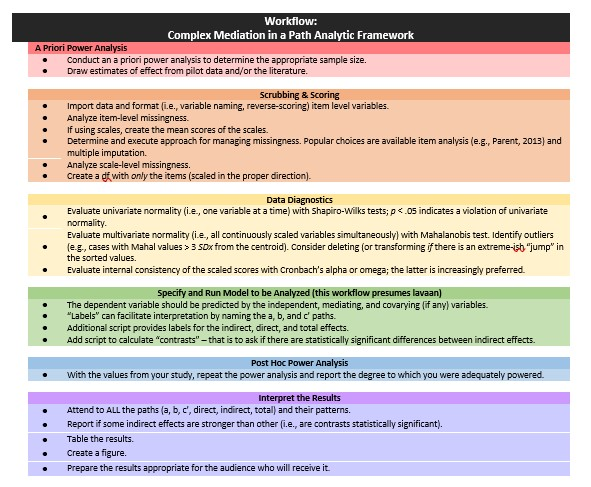
\includegraphics{images/CompMed/CompMedWorkflow.jpg}
\caption{A colorful image of a workflow for complex mediation}
\end{figure}

Conducting a parallel or serial (i.e., complex) mediation involves the following steps:

\begin{enumerate}
\def\labelenumi{\arabic{enumi}.}
\tightlist
\item
  Conducting an a priori power analysis to determine the appropriate sample size.

  \begin{itemize}
  \tightlist
  \item
    This will require estimates of effect that are drawn from pilot data, the literature, or both.
  \end{itemize}
\item
  \href{https://lhbikos.github.io/ReC_MultivModel/scrub.html}{Scrubbing} and \href{https://lhbikos.github.io/ReC_MultivModel/score.html}{scoring} the data.

  \begin{itemize}
  \tightlist
  \item
    Guidelines for such are presented in the respective lessons.
  \end{itemize}
\item
  Conducting data diagnostics, this includes:

  \begin{itemize}
  \tightlist
  \item
    item and scale level missingness,
  \item
    internal consistency coefficients (e.g., alphas or omegas) for scale scores,
  \item
    univariate and multivariate normality
  \end{itemize}
\item
  Specifying and running the model (this lesson presumes it will with the R package, \emph{lavaan}).

  \begin{itemize}
  \tightlist
  \item
    The dependent variable should be predicted by the independent, mediating, and covarying (if any) variables.
  \item
    ``Labels'' can facilitate interpretation by naming the a, b, and c' paths.
  \item
    Additional script provides labels for the indirect, direct, and total effects.
  \item
    With multiple indirect effects, specify contrasts to see if they are statistically significantly different form each other.
  \end{itemize}
\item
  Conducting a post hoc power analysis.

  \begin{itemize}
  \tightlist
  \item
    Informed by your own results, you can see if you were adequately powered to detect a statistically significant effect, if, in fact, one exists.
  \end{itemize}
\item
  Interpret and report the results.

  \begin{itemize}
  \tightlist
  \item
    Interpret ALL the paths and their patterns.
  \item
    Report if some indirect effects are stronger than others (i.e., results of the contrasts).
  \item
    Create a table and figure.
  \item
    Prepare the results in a manner that is useful to your audience.
  \end{itemize}
\end{enumerate}

\hypertarget{parallel-mediation}{%
\section{Parallel Mediation}\label{parallel-mediation}}

\textbf{Parallel multiple mediation}: An antecedent variable X is modeled as influencing consequent Y directly as well as indirectly through two or more mediators, with the condition that no mediator causally influences another \citep[p.~161]{hayes_more_2022}

With multiple mediation we introduce additional effects:

\begin{itemize}
\tightlist
\item
  \emph{Direct effect}, \(c'\) (this is not new) quantifies how much two cases that differ by a unit on X are estimated to differ on Y -- independent of all mediators.
\item
  \emph{Specific indirect effect}, \(a_{i}b_{i}\), the individual mediated effects
\item
  \emph{Total indirect effects }, \(\sum_{i=1}^{k}a_{i}b_{i}\) the sum of the values of the specific indirect effects. The total indirect effect can also be calculated by subtracting the direct effects from the total effects: \(c - c'\)
\item
  \emph{Total effect of X on Y}, \(c = c' + \sum_{i=1}^{k}a_{i}b_{i}\) (also not new) the sum of the direct and indirect effects. The total effect can also be estimated by regressing Y on X alone.
\item
  \emph{Contrasts} allow us to directly compare separate mediating effects to see if one indirect effect is stronger than the other.
\end{itemize}

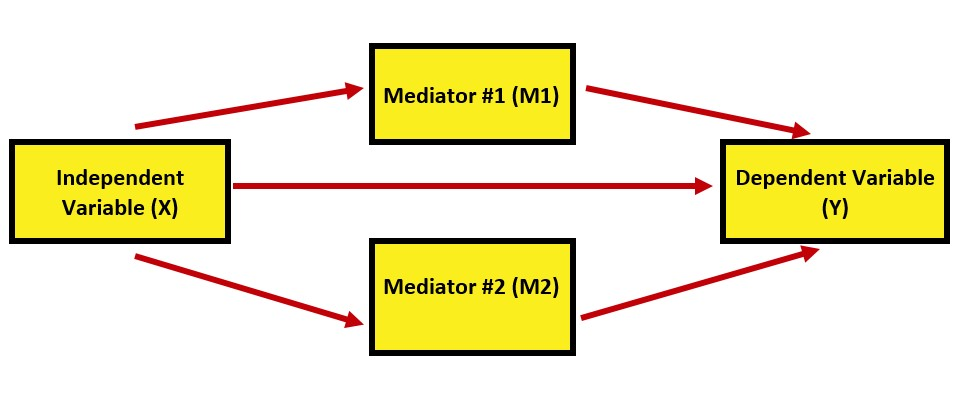
\includegraphics{images/CompMed/ParaMed.jpg} In this parallel model, we can describe these effects this way:

\begin{itemize}
\tightlist
\item
  \emph{Direct effect}: The effect of IV on the DV, accounting for two mediators (indirect effects) in the model.
\item
  \emph{Specific indirect effects}: There are indirect (or mediating) paths from the IV to the DV; through M1 and M2, respectively.
\item
  \emph{Total indirect effect of X on Y}: A sum of the value of indirect effects through the specific indirect effects (M1 and M2).
\item
  \emph{Total effect}: The sum of the direct and indirect effects. Also calculated by regressing Y (dependent variable) on X (independent variable) alone, without any other variables in the model.
\end{itemize}

Recall that for a complex mediation to be parallel, there can be no causal links between mediators. This is true in this example.

\hypertarget{a-mechanical-example}{%
\subsection{A Mechanical Example}\label{a-mechanical-example}}

Let's work a mechanical example with simulated data that assures a statistically significant outcome. Credit to this example is from the Paulo Toffanin website \citep{toffanin_multiple-mediator_2017}.

We can bake our own data by updating the script we used in simple mediation to add a second mediator.

\hypertarget{data-simulation-1}{%
\subsubsection{Data Simulation}\label{data-simulation-1}}

\begin{Shaded}
\begin{Highlighting}[]
\CommentTok{\# Concerned that identical variable names across book chapters may be}
\CommentTok{\# problematic, I\textquotesingle{}m adding \textquotesingle{}p\textquotesingle{} in front the \textquotesingle{}Data\textquotesingle{} variable.}
\FunctionTok{set.seed}\NormalTok{(}\DecValTok{230925}\NormalTok{)}
\NormalTok{X }\OtherTok{\textless{}{-}} \FunctionTok{rnorm}\NormalTok{(}\DecValTok{100}\NormalTok{)}
\NormalTok{M1 }\OtherTok{\textless{}{-}} \FloatTok{0.5} \SpecialCharTok{*}\NormalTok{ X }\SpecialCharTok{+} \FunctionTok{rnorm}\NormalTok{(}\DecValTok{100}\NormalTok{)}
\NormalTok{M2 }\OtherTok{\textless{}{-}} \SpecialCharTok{{-}}\FloatTok{0.35} \SpecialCharTok{*}\NormalTok{ X }\SpecialCharTok{+} \FunctionTok{rnorm}\NormalTok{(}\DecValTok{100}\NormalTok{)}
\NormalTok{Y }\OtherTok{\textless{}{-}} \FloatTok{0.7} \SpecialCharTok{*}\NormalTok{ M2 }\SpecialCharTok{+} \FloatTok{0.48} \SpecialCharTok{*}\NormalTok{ M1 }\SpecialCharTok{+} \FunctionTok{rnorm}\NormalTok{(}\DecValTok{100}\NormalTok{)}
\NormalTok{pData }\OtherTok{\textless{}{-}} \FunctionTok{data.frame}\NormalTok{(}\AttributeTok{X =}\NormalTok{ X, }\AttributeTok{Y =}\NormalTok{ Y, }\AttributeTok{M1 =}\NormalTok{ M1, }\AttributeTok{M2 =}\NormalTok{ M2)}
\end{Highlighting}
\end{Shaded}

Using what we learned in conducting a simple mediation in \emph{lavaan}, we can look at the figure of our proposed model and \emph{backwardstrace} the paths to write the code.

Remember\ldots{}

\begin{itemize}
\item
  The model exists between 2 single quotation marks (the odd looking ' and ' at the beginning and end).
\item
  You can write the Y as I have done in the R chunk below, or you can write the Y separately from each arrow, such as

  \begin{itemize}
  \tightlist
  \item
    Y \textasciitilde{} b1*M1
  \item
    Y \textasciitilde{} b2*M2
  \item
    Y \textasciitilde{} c\_p*X
  \end{itemize}
\item
  Everything else transfers from our simple mediation, remember that

  \begin{itemize}
  \tightlist
  \item
    the asterisk (``*``) allows us to assign labels (a1, a2, b1, b2, etc.) to the paths; these are helpful for intuitive interpretation
  \item
    that eyes/nose notation (:=) is used when creating a new variable that is a function of variables in the model, but not in the dataset (i.e., the a and b path).
  \item
    in traditional mediation speak, the direct path from X to Y is c' (c prime) and the total effect of X to Y (with nothing else in the model) is just c.~Hence the c\_p label for c prime.
  \end{itemize}
\item
  Something new: the \emph{contrast} statement (only one in this example, but you could have more) allows us to compare the indirect effects to each other. We specify it in the lavaan model, but then need to test it in a subsequent set of script.
\item
  \emph{Note}: In the online example, the writer adds code to correlate M1 and M2. This didn't/doesn't seem right to me and then, later, when we amend it to be a serial model, it made even less sense to have them be correlated.
\end{itemize}

\hypertarget{specifying-lavaan-code}{%
\subsubsection{\texorpdfstring{Specifying \emph{lavaan} code}{Specifying lavaan code}}\label{specifying-lavaan-code}}

\begin{Shaded}
\begin{Highlighting}[]
\NormalTok{parallel\_med }\OtherTok{\textless{}{-}} \StringTok{"}
\StringTok{    Y \textasciitilde{} b1*M1 + b2*M2 + c\_p*X}
\StringTok{    M1 \textasciitilde{} a1*X}
\StringTok{    M2 \textasciitilde{} a2*X}
\StringTok{    }
\StringTok{    indirect1 := a1 * b1}
\StringTok{    indirect2 := a2 * b2}
\StringTok{    contrast := indirect1 {-} indirect2}
\StringTok{    total\_indirects := indirect1 + indirect2}
\StringTok{    total\_c    := c\_p + (indirect1) + (indirect2)}
\StringTok{    direct := c\_p}
\StringTok{ "}
\FunctionTok{set.seed}\NormalTok{(}\DecValTok{230925}\NormalTok{)  }\CommentTok{\#needed for reproducibility especially when specifying bootstrapped confidence intervals}
\NormalTok{parallel\_fit }\OtherTok{\textless{}{-}}\NormalTok{ lavaan}\SpecialCharTok{::}\FunctionTok{sem}\NormalTok{(parallel\_med, }\AttributeTok{data =}\NormalTok{ pData, }\AttributeTok{se =} \StringTok{"bootstrap"}\NormalTok{,}
    \AttributeTok{missing =} \StringTok{"fiml"}\NormalTok{, }\AttributeTok{bootstrap =} \DecValTok{1000}\NormalTok{)}
\NormalTok{pfit\_sum }\OtherTok{\textless{}{-}}\NormalTok{ lavaan}\SpecialCharTok{::}\FunctionTok{summary}\NormalTok{(parallel\_fit, }\AttributeTok{standardized =} \ConstantTok{TRUE}\NormalTok{, }\AttributeTok{rsq =}\NormalTok{ T,}
    \AttributeTok{fit =} \ConstantTok{TRUE}\NormalTok{, }\AttributeTok{ci =} \ConstantTok{TRUE}\NormalTok{)}
\NormalTok{pfit\_ParEsts }\OtherTok{\textless{}{-}}\NormalTok{ lavaan}\SpecialCharTok{::}\FunctionTok{parameterEstimates}\NormalTok{(parallel\_fit, }\AttributeTok{boot.ci.type =} \StringTok{"bca.simple"}\NormalTok{,}
    \AttributeTok{standardized =} \ConstantTok{TRUE}\NormalTok{)}
\NormalTok{pfit\_sum}
\end{Highlighting}
\end{Shaded}

\begin{verbatim}
## lavaan 0.6.16 ended normally after 1 iteration
## 
##   Estimator                                         ML
##   Optimization method                           NLMINB
##   Number of model parameters                        11
## 
##   Number of observations                           100
##   Number of missing patterns                         1
## 
## Model Test User Model:
##                                                       
##   Test statistic                                 2.475
##   Degrees of freedom                                 1
##   P-value (Chi-square)                           0.116
## 
## Model Test Baseline Model:
## 
##   Test statistic                               126.642
##   Degrees of freedom                                 6
##   P-value                                        0.000
## 
## User Model versus Baseline Model:
## 
##   Comparative Fit Index (CFI)                    0.988
##   Tucker-Lewis Index (TLI)                       0.927
##                                                       
##   Robust Comparative Fit Index (CFI)             0.988
##   Robust Tucker-Lewis Index (TLI)                0.927
## 
## Loglikelihood and Information Criteria:
## 
##   Loglikelihood user model (H0)               -433.660
##   Loglikelihood unrestricted model (H1)       -432.423
##                                                       
##   Akaike (AIC)                                 889.321
##   Bayesian (BIC)                               917.977
##   Sample-size adjusted Bayesian (SABIC)        883.237
## 
## Root Mean Square Error of Approximation:
## 
##   RMSEA                                          0.121
##   90 Percent confidence interval - lower         0.000
##   90 Percent confidence interval - upper         0.322
##   P-value H_0: RMSEA <= 0.050                    0.161
##   P-value H_0: RMSEA >= 0.080                    0.772
##                                                       
##   Robust RMSEA                                   0.121
##   90 Percent confidence interval - lower         0.000
##   90 Percent confidence interval - upper         0.322
##   P-value H_0: Robust RMSEA <= 0.050             0.161
##   P-value H_0: Robust RMSEA >= 0.080             0.772
## 
## Standardized Root Mean Square Residual:
## 
##   SRMR                                           0.046
## 
## Parameter Estimates:
## 
##   Standard errors                            Bootstrap
##   Number of requested bootstrap draws             1000
##   Number of successful bootstrap draws            1000
## 
## Regressions:
##                    Estimate  Std.Err  z-value  P(>|z|) ci.lower ci.upper
##   Y ~                                                                   
##     M1        (b1)    0.456    0.107    4.243    0.000    0.241    0.667
##     M2        (b2)    0.743    0.075    9.972    0.000    0.605    0.894
##     X        (c_p)    0.030    0.099    0.305    0.760   -0.161    0.221
##   M1 ~                                                                  
##     X         (a1)    0.510    0.081    6.308    0.000    0.353    0.657
##   M2 ~                                                                  
##     X         (a2)   -0.381    0.126   -3.014    0.003   -0.630   -0.129
##    Std.lv  Std.all
##                   
##     0.456    0.383
##     0.743    0.693
##     0.030    0.025
##                   
##     0.510    0.502
##                   
##    -0.381   -0.338
## 
## Intercepts:
##                    Estimate  Std.Err  z-value  P(>|z|) ci.lower ci.upper
##    .Y                 0.113    0.098    1.155    0.248   -0.088    0.297
##    .M1               -0.089    0.099   -0.897    0.370   -0.279    0.098
##    .M2                0.017    0.121    0.139    0.889   -0.215    0.273
##    Std.lv  Std.all
##     0.113    0.083
##    -0.089   -0.078
##     0.017    0.013
## 
## Variances:
##                    Estimate  Std.Err  z-value  P(>|z|) ci.lower ci.upper
##    .Y                 0.855    0.106    8.031    0.000    0.622    1.035
##    .M1                0.970    0.118    8.193    0.000    0.728    1.191
##    .M2                1.415    0.181    7.815    0.000    1.048    1.742
##    Std.lv  Std.all
##     0.855    0.465
##     0.970    0.748
##     1.415    0.886
## 
## R-Square:
##                    Estimate
##     Y                 0.535
##     M1                0.252
##     M2                0.114
## 
## Defined Parameters:
##                    Estimate  Std.Err  z-value  P(>|z|) ci.lower ci.upper
##     indirect1         0.233    0.068    3.435    0.001    0.110    0.376
##     indirect2        -0.283    0.094   -3.026    0.002   -0.473   -0.094
##     contrast          0.516    0.103    5.001    0.000    0.307    0.712
##     total_indircts   -0.051    0.127   -0.400    0.689   -0.302    0.198
##     total_c          -0.021    0.131   -0.157    0.876   -0.277    0.238
##     direct            0.030    0.099    0.305    0.760   -0.161    0.221
##    Std.lv  Std.all
##     0.233    0.192
##    -0.283   -0.234
##     0.516    0.426
##    -0.051   -0.042
##    -0.021   -0.017
##     0.030    0.025
\end{verbatim}

\begin{Shaded}
\begin{Highlighting}[]
\NormalTok{pfit\_ParEsts}
\end{Highlighting}
\end{Shaded}

\begin{verbatim}
##                lhs op                         rhs           label    est    se
## 1                Y  ~                          M1              b1  0.456 0.107
## 2                Y  ~                          M2              b2  0.743 0.075
## 3                Y  ~                           X             c_p  0.030 0.099
## 4               M1  ~                           X              a1  0.510 0.081
## 5               M2  ~                           X              a2 -0.381 0.126
## 6                Y ~~                           Y                  0.855 0.106
## 7               M1 ~~                          M1                  0.970 0.118
## 8               M2 ~~                          M2                  1.415 0.181
## 9                X ~~                           X                  1.253 0.000
## 10               Y ~1                                              0.113 0.098
## 11              M1 ~1                                             -0.089 0.099
## 12              M2 ~1                                              0.017 0.121
## 13               X ~1                                              0.009 0.000
## 14       indirect1 :=                       a1*b1       indirect1  0.233 0.068
## 15       indirect2 :=                       a2*b2       indirect2 -0.283 0.094
## 16        contrast :=         indirect1-indirect2        contrast  0.516 0.103
## 17 total_indirects :=         indirect1+indirect2 total_indirects -0.051 0.127
## 18         total_c := c_p+(indirect1)+(indirect2)         total_c -0.021 0.131
## 19          direct :=                         c_p          direct  0.030 0.099
##         z pvalue ci.lower ci.upper std.lv std.all std.nox
## 1   4.243  0.000    0.227    0.658  0.456   0.383   0.383
## 2   9.972  0.000    0.597    0.890  0.743   0.693   0.693
## 3   0.305  0.760   -0.160    0.227  0.030   0.025   0.022
## 4   6.308  0.000    0.356    0.660  0.510   0.502   0.448
## 5  -3.014  0.003   -0.624   -0.125 -0.381  -0.338  -0.302
## 6   8.031  0.000    0.671    1.078  0.855   0.465   0.465
## 7   8.193  0.000    0.758    1.248  0.970   0.748   0.748
## 8   7.815  0.000    1.113    1.834  1.415   0.886   0.886
## 9      NA     NA    1.253    1.253  1.253   1.000   1.253
## 10  1.155  0.248   -0.078    0.301  0.113   0.083   0.083
## 11 -0.897  0.370   -0.286    0.094 -0.089  -0.078  -0.078
## 12  0.139  0.889   -0.234    0.240  0.017   0.013   0.013
## 13     NA     NA    0.009    0.009  0.009   0.008   0.009
## 14  3.435  0.001    0.124    0.395  0.233   0.192   0.172
## 15 -3.026  0.002   -0.483   -0.105 -0.283  -0.234  -0.209
## 16  5.001  0.000    0.299    0.708  0.516   0.426   0.380
## 17 -0.400  0.689   -0.304    0.193 -0.051  -0.042  -0.037
## 18 -0.157  0.876   -0.251    0.252 -0.021  -0.017  -0.015
## 19  0.305  0.760   -0.160    0.227  0.030   0.025   0.022
\end{verbatim}

\hypertarget{a-note-on-indirect-effects-and-confidence-intervals}{%
\subsubsection{A note on indirect effects and confidence intervals}\label{a-note-on-indirect-effects-and-confidence-intervals}}

Before we move onto interpretation, I want to stop and look at both \(p\) values and confidence intervals. Especially with Hayes \citeyearpar{hayes_more_2022} PROCESS macro, there is a great deal of emphasis on the use of bootstrapped confidence intervals to determine the statistical significance of the indirect effects. In fact, PROCESS output has (at least historically) not provided \(p\) values with the indirect effects. This is because, especially in the ordinary least squares context, bias-corrected bootstrapped confidence intervals are more powerful (i.e., they are more likely to support a statistically significant result) than \(p\) values.

An excellent demonstration of this phenomena was provided by Mallinckrodt et al. \citeyearpar{mallinckrodt_advances_2006} where they compared confidence intervals produced by the normal theory method to those that are bias corrected. The bias corrected intervals were more powerful to determining if there were statistically significant indirect effects.

The method we have specified in \emph{lavaan} produced bias-corrected confidence intervals. The \(p\) values and corresponding confidence intervals should be consistent with each other. That is, if \(p\) \textless{} .05, then the CI95s should not pass through zero. Of course we can always check to be certain this is true. For this reason, I will report \(p\) values in my results. There are reviewers, though, who may prefer that you report CI95s (or both).

\hypertarget{figures-and-tables}{%
\subsubsection{Figures and Tables}\label{figures-and-tables}}

To assist in table preparation, it is possible to export the results to a .csv file that can be manipulated in Excel, Microsoft Word, or other program to prepare an APA style table.

\begin{Shaded}
\begin{Highlighting}[]
\FunctionTok{write.csv}\NormalTok{(pfit\_ParEsts, }\AttributeTok{file =} \StringTok{"pfit\_ParEsts.csv"}\NormalTok{)}
\end{Highlighting}
\end{Shaded}

We can use the package \href{https://cjvanlissa.github.io/tidySEM/articles/Plotting_graphs.html}{tidySEM} to create a figure that includes the values on the path.

Here's what the base package gets us

\begin{Shaded}
\begin{Highlighting}[]
\CommentTok{\# only worked when I used the library to turn on all these pkgs}
\FunctionTok{library}\NormalTok{(lavaan)}
\FunctionTok{library}\NormalTok{(dplyr)}
\FunctionTok{library}\NormalTok{(ggplot2)}
\FunctionTok{library}\NormalTok{(tidySEM)}
\NormalTok{tidySEM}\SpecialCharTok{::}\FunctionTok{graph\_sem}\NormalTok{(}\AttributeTok{model =}\NormalTok{ parallel\_fit)}
\end{Highlighting}
\end{Shaded}

\includegraphics{06-ComplexMed_files/figure-latex/unnamed-chunk-6-1.pdf}

We can create model that communicates more intuitively with a little tinkering. First, let's retrieve the current ``map'' of the layout.

\begin{Shaded}
\begin{Highlighting}[]
\NormalTok{tidySEM}\SpecialCharTok{::}\FunctionTok{get\_layout}\NormalTok{(parallel\_fit)}
\end{Highlighting}
\end{Shaded}

\begin{verbatim}
##      [,1] [,2] [,3]
## [1,] NA   "X"  NA  
## [2,] "M1" "M2" "Y" 
## attr(,"class")
## [1] "layout_matrix" "matrix"        "array"
\end{verbatim}

To create the figure I showed at the beginning of the chapter, we will want three rows and three columns.

\begin{Shaded}
\begin{Highlighting}[]
\NormalTok{parallel\_map }\OtherTok{\textless{}{-}}\NormalTok{ tidySEM}\SpecialCharTok{::}\FunctionTok{get\_layout}\NormalTok{(}\StringTok{""}\NormalTok{, }\StringTok{"M1"}\NormalTok{, }\StringTok{""}\NormalTok{, }\StringTok{"X"}\NormalTok{, }\StringTok{""}\NormalTok{, }\StringTok{"Y"}\NormalTok{, }\StringTok{""}\NormalTok{, }\StringTok{"M2"}\NormalTok{,}
    \StringTok{""}\NormalTok{, }\AttributeTok{rows =} \DecValTok{3}\NormalTok{)}
\NormalTok{parallel\_map}
\end{Highlighting}
\end{Shaded}

\begin{verbatim}
##      [,1] [,2] [,3]
## [1,] ""   "M1" ""  
## [2,] "X"  ""   "Y" 
## [3,] ""   "M2" ""  
## attr(,"class")
## [1] "layout_matrix" "matrix"        "array"
\end{verbatim}

We can update our figure by supplying this new map and adjusting the object and text sizes.

\begin{Shaded}
\begin{Highlighting}[]
\NormalTok{tidySEM}\SpecialCharTok{::}\FunctionTok{graph\_sem}\NormalTok{(parallel\_fit, }\AttributeTok{layout =}\NormalTok{ parallel\_map, }\AttributeTok{rect\_width =} \FloatTok{1.5}\NormalTok{,}
    \AttributeTok{rect\_height =} \FloatTok{1.25}\NormalTok{, }\AttributeTok{spacing\_x =} \DecValTok{2}\NormalTok{, }\AttributeTok{spacing\_y =} \DecValTok{3}\NormalTok{, }\AttributeTok{text\_size =} \FloatTok{4.5}\NormalTok{)}
\end{Highlighting}
\end{Shaded}

\includegraphics{06-ComplexMed_files/figure-latex/unnamed-chunk-9-1.pdf}

There are a number of ways to tabalize the data. You might be surprised to learn that a number of articles that analyze mediating effects focus their presentation on those values and not the traditional intercepts and B weights. This is the approach I have taken in this chapter.

\textbf{Table 1 }

\begin{longtable}[]{@{}
  >{\raggedright\arraybackslash}p{(\columnwidth - 0\tabcolsep) * \real{1.0000}}@{}}
\toprule\noalign{}
\begin{minipage}[b]{\linewidth}\raggedright
Model Coefficients Assessing M1 and M2 as Parallel Mediators Between X and Y
\end{minipage} \\
\midrule\noalign{}
\endhead
\bottomrule\noalign{}
\endlastfoot
\end{longtable}

\begin{longtable}[]{@{}
  >{\raggedright\arraybackslash}p{(\columnwidth - 8\tabcolsep) * \real{0.4000}}
  >{\centering\arraybackslash}p{(\columnwidth - 8\tabcolsep) * \real{0.1286}}
  >{\centering\arraybackslash}p{(\columnwidth - 8\tabcolsep) * \real{0.1429}}
  >{\centering\arraybackslash}p{(\columnwidth - 8\tabcolsep) * \real{0.1143}}
  >{\centering\arraybackslash}p{(\columnwidth - 8\tabcolsep) * \real{0.2143}}@{}}
\toprule\noalign{}
\begin{minipage}[b]{\linewidth}\raggedright
Predictor
\end{minipage} & \begin{minipage}[b]{\linewidth}\centering
\(B\)
\end{minipage} & \begin{minipage}[b]{\linewidth}\centering
\(SE_{B}\)
\end{minipage} & \begin{minipage}[b]{\linewidth}\centering
\(p\)
\end{minipage} & \begin{minipage}[b]{\linewidth}\centering
\(R^2\)
\end{minipage} \\
\midrule\noalign{}
\endhead
\bottomrule\noalign{}
\endlastfoot
\end{longtable}

\begin{longtable}[]{@{}
  >{\raggedright\arraybackslash}p{(\columnwidth - 8\tabcolsep) * \real{0.4000}}
  >{\centering\arraybackslash}p{(\columnwidth - 8\tabcolsep) * \real{0.1286}}
  >{\centering\arraybackslash}p{(\columnwidth - 8\tabcolsep) * \real{0.1429}}
  >{\centering\arraybackslash}p{(\columnwidth - 8\tabcolsep) * \real{0.1143}}
  >{\centering\arraybackslash}p{(\columnwidth - 8\tabcolsep) * \real{0.2143}}@{}}
\toprule\noalign{}
\begin{minipage}[b]{\linewidth}\raggedright
M1
\end{minipage} & \begin{minipage}[b]{\linewidth}\centering
\end{minipage} & \begin{minipage}[b]{\linewidth}\centering
\end{minipage} & \begin{minipage}[b]{\linewidth}\centering
\end{minipage} & \begin{minipage}[b]{\linewidth}\centering
.25
\end{minipage} \\
\midrule\noalign{}
\endhead
\bottomrule\noalign{}
\endlastfoot
Constant & -0.089 & 0.099 & 0.370 & \\
X (\(a_1\)) & 0.510 & 0.081 & \textless0.001 & \\
\end{longtable}

\begin{longtable}[]{@{}
  >{\raggedright\arraybackslash}p{(\columnwidth - 8\tabcolsep) * \real{0.4000}}
  >{\centering\arraybackslash}p{(\columnwidth - 8\tabcolsep) * \real{0.1286}}
  >{\centering\arraybackslash}p{(\columnwidth - 8\tabcolsep) * \real{0.1429}}
  >{\centering\arraybackslash}p{(\columnwidth - 8\tabcolsep) * \real{0.1143}}
  >{\centering\arraybackslash}p{(\columnwidth - 8\tabcolsep) * \real{0.2143}}@{}}
\toprule\noalign{}
\begin{minipage}[b]{\linewidth}\raggedright
M2
\end{minipage} & \begin{minipage}[b]{\linewidth}\centering
\end{minipage} & \begin{minipage}[b]{\linewidth}\centering
\end{minipage} & \begin{minipage}[b]{\linewidth}\centering
\end{minipage} & \begin{minipage}[b]{\linewidth}\centering
.11
\end{minipage} \\
\midrule\noalign{}
\endhead
\bottomrule\noalign{}
\endlastfoot
Constant & 0.017 & 0.121 & 0.889 & \\
X (\(a_2\)) & -0.381 & 0.126 & 0.003 & \\
\end{longtable}

\begin{longtable}[]{@{}
  >{\raggedright\arraybackslash}p{(\columnwidth - 8\tabcolsep) * \real{0.4000}}
  >{\centering\arraybackslash}p{(\columnwidth - 8\tabcolsep) * \real{0.1286}}
  >{\centering\arraybackslash}p{(\columnwidth - 8\tabcolsep) * \real{0.1429}}
  >{\centering\arraybackslash}p{(\columnwidth - 8\tabcolsep) * \real{0.1143}}
  >{\centering\arraybackslash}p{(\columnwidth - 8\tabcolsep) * \real{0.2143}}@{}}
\toprule\noalign{}
\begin{minipage}[b]{\linewidth}\raggedright
DV
\end{minipage} & \begin{minipage}[b]{\linewidth}\centering
\end{minipage} & \begin{minipage}[b]{\linewidth}\centering
\end{minipage} & \begin{minipage}[b]{\linewidth}\centering
\end{minipage} & \begin{minipage}[b]{\linewidth}\centering
.54
\end{minipage} \\
\midrule\noalign{}
\endhead
\bottomrule\noalign{}
\endlastfoot
Constant & 0.113 & 0.098 & 0.248 & \\
M1 (\(b_1\)) & 0.456 & 0.107 & \textless0.001 & \\
M2 (\(b_2\)) & 0.743 & 0.075 & \textless0.001 & \\
X (\(c'\)) & 0.030 & 0.099 & 0.760 & \\
\end{longtable}

\begin{longtable}[]{@{}
  >{\raggedright\arraybackslash}p{(\columnwidth - 8\tabcolsep) * \real{0.4000}}
  >{\centering\arraybackslash}p{(\columnwidth - 8\tabcolsep) * \real{0.1286}}
  >{\centering\arraybackslash}p{(\columnwidth - 8\tabcolsep) * \real{0.1429}}
  >{\centering\arraybackslash}p{(\columnwidth - 8\tabcolsep) * \real{0.1143}}
  >{\centering\arraybackslash}p{(\columnwidth - 8\tabcolsep) * \real{0.2143}}@{}}
\toprule\noalign{}
\begin{minipage}[b]{\linewidth}\raggedright
Summary of Effects
\end{minipage} & \begin{minipage}[b]{\linewidth}\centering
\(B\)
\end{minipage} & \begin{minipage}[b]{\linewidth}\centering
\(SE_{B}\)
\end{minipage} & \begin{minipage}[b]{\linewidth}\centering
\(p\)
\end{minipage} & \begin{minipage}[b]{\linewidth}\centering
95\% CI
\end{minipage} \\
\midrule\noalign{}
\endhead
\bottomrule\noalign{}
\endlastfoot
Total & -0.021 & 0.131 & 0.876 & -0.251, 0.252 \\
Indirect 1 (\(a_1\) * \(a_2\)) & 0.233 & 0.068 & 0.001 & 0.124, 0.395 \\
Indirect 2 (\(b_1\) * \(b_2\)) & -0.283 & 0.094 & 0.002 & -0.483, -0.105 \\
Total indirects & -0.051 & 0.127 & 0.689 & -0.304, 0.193 \\
Contrast (Ind1 - Ind2) & 0.516 & 0.103 & \textless0.001 & 0.299, 0.708 \\
\end{longtable}

\begin{longtable}[]{@{}
  >{\raggedright\arraybackslash}p{(\columnwidth - 0\tabcolsep) * \real{1.0000}}@{}}
\toprule\noalign{}
\endhead
\bottomrule\noalign{}
\endlastfoot
\emph{Note}. The significance of the indirect effects was calculated with bootstrapped, bias-corrected, confidence intervals (.95). \\
\end{longtable}

\hypertarget{apa-style-writeup}{%
\subsubsection{APA Style Writeup}\label{apa-style-writeup}}

You may notice that my write-up includes almost no statistical output. This is consistent with APA style that avoids redundancy in text and table. When I want to emphasize a specific result, I may duplicate some output in the text.

\begin{quote}
A model of parallel multiple mediation was analyzed examining the degree to which importance of M1 and M2 mediated the relation of X on Y. Hayes \citeyearpar{hayes_more_2022} recommended this strategy over simple mediation models because it allows for all mediators to be examined, simultaneously. The resultant direct and indirect values for each path account for other mediation paths. Using the \emph{lavaan (v. 0.6-16)} package in R, coefficients for specific indirect, total indirect, direct, and total were computed. Path coefficients refer to regression weights, or slopes, of the expected changes in the dependent variable given a unit change in the independent variables.
\end{quote}

\begin{quote}
Results (depicted in Figure 1 and presented in Table 1) suggest that 54\% of the variance in Y is accounted for by the model. Neither the total nor direct effect of X on Y were statistically significant. In contrast, both indirect effects were statistically significant. A pairwise comparison of the specific indirect effects indicated that the strength of the effects were statistically significantly different from each other. In summary, the effect of X on Y is mediated through M1 and M2, with a stronger influence through M2.
\end{quote}

You may notice this write-up included only one statistic. I offered this as an example of avoiding redundancy in text and table. When tables and figures convey maximal information, the results section may be used to describe the patterns -- including numbers when they reduce the cognitive load for the readers and reviewers.

Let's turn now to the research vignette and work an example with simulated data from that example. Because the research vignette use an entirely new set of output I will either restart R or clear my environment so that there are a few less objects ``in the way.''

\hypertarget{research-vignette-5}{%
\subsection{Research Vignette}\label{research-vignette-5}}

The research vignette comes from the Lewis, Williams, Peppers, and Gadson's \citeyearpar{lewis_applying_2017} study titled, ``Applying Intersectionality to Explore the Relations Between Gendered Racism and Health Among Black Women.'' The study was published in the Journal of Counseling Psychology. Participants were 231 Black women who completed an online survey.

Variables used in the study included:

\begin{itemize}
\item
  \textbf{GRMS}: Gendered Racial Microaggressions Scale \citep{lewis_construction_2015} is a 26-item scale that assesses the frequency of nonverbal, verbal, and behavioral negative racial and gender slights experienced by Black women. Scaling is along six points ranging from 0 (\emph{never}) to 5 (\emph{once a week or more}). Higher scores indicate a greater frequency of gendered racial microaggressions. An example item is, ``Someone has tried to `put me in my place.'\,''
\item
  \textbf{MntlHlth} and \textbf{PhysHlth}: Short Form Health Survey - Version 2 \citep{ware_comparison_1995} is a 12-item scale used to report self-reported mental (six items) and physical health (six items). Although the article did not specify, when this scale is used in other contexts \citep[e.g.,][]{kim_racial_2017}, a 6-point scale has been reported. Higher scores indicate higher mental health (e.g., little or no psychological distress) and physical health (e.g., little or no reported symptoms in physical functioning). An example of an item assessing mental health was, ``How much of the time during the last 4 weeks have you felt calm and peaceful?''; an example of a physical health item was, ``During the past 4 weeks, how much did pain interfere with your normal work?''
\item
  \textbf{Sprtlty}, \textbf{SocSup}, \textbf{Engmgt}, and \textbf{DisEngmt} are four subscales from the Brief Coping with Problems Experienced Inventory \citep{carver_you_1997}. The 28 items on this scale are presented on a 4-point scale ranging from 1 (\emph{I usually do not do this at all}) to 4(\emph{I usually do this a lot}). Higher scores indicate a respondents' tendency to engage in a particular strategy. Instructions were modified to ask how the female participants responded to recent experiences of racism and sexism as Black women. The four subscales included spirituality (religion, acceptance, planning), interconnectedness/social support (vent emotions, emotional support,instrumental social support), problem-oriented/engagement coping (active coping, humor, positive reinterpretation/positive reframing), and disengagement coping (behavioral disengagement, substance abuse, denial, self-blame, self-distraction).
\item
  \textbf{GRIcntlty}: The Multidimensional Inventory of Black Identity Centrality subscale \citep{sellers_multidimensional_nodate} was modified to measure the intersection of racial and gender identity centrality. The scale included 10 items scaled from 1 (\emph{strongly disagree}) to 7 (\emph{strongly agree}). An example item was, ``Being a \emph{Black woman} is important to my self-image.'' Higher scores indicated higher levels of gendered racial identity centrality.
\end{itemize}

\hypertarget{data-simulation-2}{%
\subsubsection{Data Simulation}\label{data-simulation-2}}

The \emph{lavaan::simulateData} function was used. If you have taken psychometrics, you may recognize the code as one that creates latent variables form item-level data. In trying to be as authentic as possible, we retrieved factor loadings from psychometrically oriented articles that evaluated the measures \citep{nadal_racial_2011, veit_structure_1983}. For all others we specified a factor loading of 0.80. We then approximated the \emph{measurement model} by specifying the correlations between the latent variable. We sourced these from the correlation matrix from the research vignette \citep{lewis_applying_2017}. The process created data with multiple decimals and values that exceeded the boundaries of the variables. For example, in all scales there were negative values. Therefore, the final element of the simulation was a linear transformation that rescaled the variables back to the range described in the journal article and rounding the values to integer (i.e., with no decimal places).

\begin{Shaded}
\begin{Highlighting}[]
\CommentTok{\#Entering the intercorrelations, means, and standard deviations from the journal article}

\NormalTok{Lewis\_generating\_model }\OtherTok{\textless{}{-}} \StringTok{\textquotesingle{}}
\StringTok{        \#\#measurement model}
\StringTok{        GRMS  =\textasciitilde{} .69*Ob1 + .69*Ob2 + .60*Ob3 + .59*Ob4 + .55*Ob5 + .55*Ob6 + .54*Ob7 + .50*Ob8 + .41*Ob9 + .41*Ob10 + .93*Ma1 + .81*Ma2 + .69*Ma3 + .67*Ma4 + .61*Ma5 + .58*Ma6 + .54*Ma7 + .59*St1 + .55*St2 + .54*St3 + .54*St4 + .51*St5 + .70*An1 + .69*An2 + .68*An3}
\StringTok{        MntlHlth  =\textasciitilde{} .8*MH1 + .8*MH2 + .8*MH3 + .8*MH4 + .8*MH5 + .8*MH6}
\StringTok{        PhysHlth  =\textasciitilde{} .8*PhH1 + .8*PhH2 + .8*PhH3 + .8*PhH4 + .8*PhH5 + .8*PhH6}
\StringTok{        Spirituality  =\textasciitilde{} .8*Spirit1 + .8*Spirit2}
\StringTok{        SocSupport  =\textasciitilde{} .8*SocS1 + .8*SocS2}
\StringTok{        Engagement  =\textasciitilde{} .8*Eng1 + .8*Eng2}
\StringTok{        Disengagement  =\textasciitilde{}  .8*dEng1 + .8*dEng2}
\StringTok{        GRIC  =\textasciitilde{} .8*Cntrlty1 + .8*Cntrlty2 + .8*Cntrlty3 + .8*Cntrlty4 + .8*Cntrlty5 + .8*Cntrlty6 + .8*Cntrlty7 + .8*Cntrlty8 + .8*Cntrlty9 + .8*Cntrlty10}
\StringTok{   }
\StringTok{        \# Means}
\StringTok{         GRMS \textasciitilde{} 1.99*1}
\StringTok{         Spirituality \textasciitilde{}2.82*1}
\StringTok{         SocSupport \textasciitilde{} 2.48*1}
\StringTok{         Engagement \textasciitilde{} 2.32*1}
\StringTok{         Disengagement \textasciitilde{} 1.75*1}
\StringTok{         GRIC \textasciitilde{} 5.71*1}
\StringTok{         MntlHlth \textasciitilde{}3.56*1 \#Lewis et al used sums instead of means, I recast as means to facilitate simulation}
\StringTok{         PhysHlth \textasciitilde{} 3.51*1 \#Lewis et al used sums instead of means, I recast as means to facilitate simulation}
\StringTok{         }
\StringTok{        \# Correlations }
\StringTok{         GRMS \textasciitilde{} 0.20*Spirituality}
\StringTok{         GRMS \textasciitilde{} 0.28*SocSupport}
\StringTok{         GRMS \textasciitilde{} 0.30*Engagement}
\StringTok{         GRMS \textasciitilde{} 0.41*Disengagement}
\StringTok{         GRMS \textasciitilde{} 0.19*GRIC}
\StringTok{         GRMS \textasciitilde{} {-}0.32*MntlHlth}
\StringTok{         GRMS \textasciitilde{} {-}0.18*PhysHlth}
\StringTok{         }
\StringTok{         Spirituality \textasciitilde{} 0.49*SocSupport}
\StringTok{         Spirituality \textasciitilde{} 0.57*Engagement}
\StringTok{         Spirituality \textasciitilde{} 0.22*Disengagement}
\StringTok{         Spirituality \textasciitilde{} 0.12*GRIC}
\StringTok{         Spirituality \textasciitilde{} {-}0.06*MntlHlth}
\StringTok{         Spirituality \textasciitilde{} {-}0.13*PhysHlth}
\StringTok{         }
\StringTok{         SocSupport \textasciitilde{} 0.46*Engagement}
\StringTok{         SocSupport \textasciitilde{} 0.26*Disengagement}
\StringTok{         SocSupport \textasciitilde{} 0.38*GRIC}
\StringTok{         SocSupport \textasciitilde{} {-}0.18*MntlHlth}
\StringTok{         SocSupport \textasciitilde{} {-}0.08*PhysHlth}
\StringTok{         }
\StringTok{         Engagement \textasciitilde{} 0.37*Disengagement}
\StringTok{         Engagement \textasciitilde{} 0.08*GRIC}
\StringTok{         Engagement \textasciitilde{} {-}0.14*MntlHlth}
\StringTok{         Engagement \textasciitilde{} {-}0.06*PhysHlth}
\StringTok{         }
\StringTok{         Disengagement \textasciitilde{} 0.05*GRIC}
\StringTok{         Disengagement \textasciitilde{} {-}0.54*MntlHlth}
\StringTok{         Disengagement \textasciitilde{} {-}0.28*PhysHlth}
\StringTok{         }
\StringTok{         GRIC \textasciitilde{} {-}0.10*MntlHlth}
\StringTok{         GRIC \textasciitilde{} 0.14*PhysHlth}
\StringTok{     }
\StringTok{         MntlHlth \textasciitilde{} 0.47*PhysHlth         }
\StringTok{        \textquotesingle{}}

\FunctionTok{set.seed}\NormalTok{(}\DecValTok{230925}\NormalTok{)}
\NormalTok{dfLewis }\OtherTok{\textless{}{-}}\NormalTok{ lavaan}\SpecialCharTok{::}\FunctionTok{simulateData}\NormalTok{(}\AttributeTok{model =}\NormalTok{ Lewis\_generating\_model,}
                              \AttributeTok{model.type =} \StringTok{"sem"}\NormalTok{,}
                              \AttributeTok{meanstructure =}\NormalTok{ T,}
                              \AttributeTok{sample.nobs=}\DecValTok{231}\NormalTok{,}
                              \AttributeTok{standardized=}\ConstantTok{FALSE}\NormalTok{)}

\CommentTok{\#used to retrieve column indices used in the rescaling script below}
\CommentTok{\#col\_index \textless{}{-} as.data.frame(colnames(dfLewis))}

\ControlFlowTok{for}\NormalTok{(i }\ControlFlowTok{in} \DecValTok{1}\SpecialCharTok{:}\FunctionTok{ncol}\NormalTok{(dfLewis))\{  }\CommentTok{\# for loop to go through each column of the dataframe }
  \ControlFlowTok{if}\NormalTok{(i }\SpecialCharTok{\textgreater{}=} \DecValTok{1} \SpecialCharTok{\&}\NormalTok{ i }\SpecialCharTok{\textless{}=} \DecValTok{25}\NormalTok{)\{   }\CommentTok{\# apply only to GRMS variables}
\NormalTok{    dfLewis[,i] }\OtherTok{\textless{}{-}}\NormalTok{ scales}\SpecialCharTok{::}\FunctionTok{rescale}\NormalTok{(dfLewis[,i], }\FunctionTok{c}\NormalTok{(}\DecValTok{0}\NormalTok{, }\DecValTok{5}\NormalTok{))}
\NormalTok{  \}}
  \ControlFlowTok{if}\NormalTok{(i }\SpecialCharTok{\textgreater{}=} \DecValTok{26} \SpecialCharTok{\&}\NormalTok{ i }\SpecialCharTok{\textless{}=} \DecValTok{37}\NormalTok{)\{   }\CommentTok{\# apply only to mental and physical health variables }
\NormalTok{    dfLewis[,i] }\OtherTok{\textless{}{-}}\NormalTok{ scales}\SpecialCharTok{::}\FunctionTok{rescale}\NormalTok{(dfLewis[,i], }\FunctionTok{c}\NormalTok{(}\DecValTok{0}\NormalTok{, }\DecValTok{6}\NormalTok{))}
\NormalTok{  \}}
  \ControlFlowTok{if}\NormalTok{(i }\SpecialCharTok{\textgreater{}=} \DecValTok{38} \SpecialCharTok{\&}\NormalTok{ i }\SpecialCharTok{\textless{}=} \DecValTok{45}\NormalTok{)\{   }\CommentTok{\# apply only to coping variables}
\NormalTok{    dfLewis[,i] }\OtherTok{\textless{}{-}}\NormalTok{ scales}\SpecialCharTok{::}\FunctionTok{rescale}\NormalTok{(dfLewis[,i], }\FunctionTok{c}\NormalTok{(}\DecValTok{1}\NormalTok{, }\DecValTok{4}\NormalTok{))}
\NormalTok{  \}}
  \ControlFlowTok{if}\NormalTok{(i }\SpecialCharTok{\textgreater{}=} \DecValTok{46} \SpecialCharTok{\&}\NormalTok{ i }\SpecialCharTok{\textless{}=} \DecValTok{55}\NormalTok{)\{   }\CommentTok{\# apply only to GRIC variables}
\NormalTok{    dfLewis[,i] }\OtherTok{\textless{}{-}}\NormalTok{ scales}\SpecialCharTok{::}\FunctionTok{rescale}\NormalTok{(dfLewis[,i], }\FunctionTok{c}\NormalTok{(}\DecValTok{1}\NormalTok{, }\DecValTok{7}\NormalTok{))}
\NormalTok{  \}}
\NormalTok{\}}

\CommentTok{\#rounding to integers so that the data resembles that which was collected}
\FunctionTok{library}\NormalTok{(tidyverse)}
\NormalTok{dfLewis }\OtherTok{\textless{}{-}}\NormalTok{ dfLewis }\SpecialCharTok{\%\textgreater{}\%} \FunctionTok{round}\NormalTok{(}\DecValTok{0}\NormalTok{) }

\CommentTok{\#quick check of my work}
\CommentTok{\#psych::describe(dfLewis) }
\end{Highlighting}
\end{Shaded}

The script below allows you to store the simulated data as a file on your computer. This is optional -- the entire lesson can be worked with the simulated data.

If you prefer the .rds format, use this script (remove the hashtags). The .rds format has the advantage of preserving any formatting of variables. A disadvantage is that you cannot open these files outside of the R environment.

Script to save the data to your computer as an .rds file.

\begin{Shaded}
\begin{Highlighting}[]
\CommentTok{\#saveRDS(dfLewis, \textquotesingle{}dfLewis.rds\textquotesingle{})  }
\end{Highlighting}
\end{Shaded}

Once saved, you could clean your environment and bring the data back in from its .csv format.

\begin{Shaded}
\begin{Highlighting}[]
\CommentTok{\#dfLewis\textless{}{-} readRDS(\textquotesingle{}dfLewis.rds\textquotesingle{})}
\end{Highlighting}
\end{Shaded}

If you prefer the .csv format (think ``Excel lite'') use this script (remove the hashtags). An advantage of the .csv format is that you can open the data outside of the R environment. A disadvantage is that it may not retain any formatting of variables

Script to save the data to your computer as a .csv file.

\begin{Shaded}
\begin{Highlighting}[]
\CommentTok{\# write.table(dfLewis, file = \textquotesingle{}dfLewis.csv\textquotesingle{}, sep = \textquotesingle{},\textquotesingle{},}
\CommentTok{\# col.names=TRUE, row.names=FALSE)}
\end{Highlighting}
\end{Shaded}

Once saved, you could clean your environment and bring the data back in from its .csv format.

\begin{Shaded}
\begin{Highlighting}[]
\CommentTok{\#dfLewis\textless{}{-} read.csv (\textquotesingle{}dfLewis.csv\textquotesingle{}, header = TRUE)}
\end{Highlighting}
\end{Shaded}

\hypertarget{scrubbing-scoring-and-data-diagnostics-1}{%
\subsection{Scrubbing, Scoring, and Data Diagnostics}\label{scrubbing-scoring-and-data-diagnostics-1}}

Because the focus of this lesson is on complex mediation, we have used simulated data. If this were real, raw, data, it would be important to \href{https://lhbikos.github.io/ReC_MultivModel/scrub.html}{scrub}, \href{https://lhbikos.github.io/ReC_MultivModel/score.html}{score}, and conduct \href{https://lhbikos.github.io/ReC_MultivModel/DataDx.html}{data diagnostics} to evaluate the suitability of the data for the proposes anlayses.

Because we are working with item level data we do need to score the scales used in the researcher's model. Because we are using simulated data and the authors already reverse coded any such items, we will omit that step.

As described in the \href{https://lhbikos.github.io/ReC_MultivModel/score.html}{Scoring} chapter, we calculate mean scores of these variables by first creating concatenated lists of variable names. Next we apply the \emph{sjstats::mean\_n} function to obtain mean scores when a given percentage (we'll specify 80\%) of variables are non-missing. Functionally, this would require the two-item variables (e.g., engagement coping and disengagement coping) to have non-missingness. We simulated a set of data that does not have missingness, none-the-less, this specification is useful in real-world settings.

Note that I am only scoring the variables used in the models demonstrated in this lesson. The remaining variables are available as practice options.

\begin{Shaded}
\begin{Highlighting}[]
\NormalTok{GRMS\_vars }\OtherTok{\textless{}{-}} \FunctionTok{c}\NormalTok{(}\StringTok{"Ob1"}\NormalTok{, }\StringTok{"Ob2"}\NormalTok{, }\StringTok{"Ob3"}\NormalTok{, }\StringTok{"Ob4"}\NormalTok{, }\StringTok{"Ob5"}\NormalTok{, }\StringTok{"Ob6"}\NormalTok{, }\StringTok{"Ob7"}\NormalTok{, }\StringTok{"Ob8"}\NormalTok{,}
    \StringTok{"Ob9"}\NormalTok{, }\StringTok{"Ob10"}\NormalTok{, }\StringTok{"Ma1"}\NormalTok{, }\StringTok{"Ma2"}\NormalTok{, }\StringTok{"Ma3"}\NormalTok{, }\StringTok{"Ma4"}\NormalTok{, }\StringTok{"Ma5"}\NormalTok{, }\StringTok{"Ma6"}\NormalTok{, }\StringTok{"Ma7"}\NormalTok{, }\StringTok{"St1"}\NormalTok{,}
    \StringTok{"St2"}\NormalTok{, }\StringTok{"St3"}\NormalTok{, }\StringTok{"St4"}\NormalTok{, }\StringTok{"St5"}\NormalTok{, }\StringTok{"An1"}\NormalTok{, }\StringTok{"An2"}\NormalTok{, }\StringTok{"An3"}\NormalTok{)}
\NormalTok{Eng\_vars }\OtherTok{\textless{}{-}} \FunctionTok{c}\NormalTok{(}\StringTok{"Eng1"}\NormalTok{, }\StringTok{"Eng2"}\NormalTok{)}
\NormalTok{dEng\_vars }\OtherTok{\textless{}{-}} \FunctionTok{c}\NormalTok{(}\StringTok{"dEng1"}\NormalTok{, }\StringTok{"dEng2"}\NormalTok{)}
\NormalTok{MntlHlth\_vars }\OtherTok{\textless{}{-}} \FunctionTok{c}\NormalTok{(}\StringTok{"MH1"}\NormalTok{, }\StringTok{"MH2"}\NormalTok{, }\StringTok{"MH3"}\NormalTok{, }\StringTok{"MH4"}\NormalTok{, }\StringTok{"MH5"}\NormalTok{, }\StringTok{"MH6"}\NormalTok{)}

\NormalTok{dfLewis}\SpecialCharTok{$}\NormalTok{GRMS }\OtherTok{\textless{}{-}}\NormalTok{ sjstats}\SpecialCharTok{::}\FunctionTok{mean\_n}\NormalTok{(dfLewis[, GRMS\_vars], }\FloatTok{0.8}\NormalTok{)}
\NormalTok{dfLewis}\SpecialCharTok{$}\NormalTok{Engmt }\OtherTok{\textless{}{-}}\NormalTok{ sjstats}\SpecialCharTok{::}\FunctionTok{mean\_n}\NormalTok{(dfLewis[, Eng\_vars], }\FloatTok{0.8}\NormalTok{)}
\NormalTok{dfLewis}\SpecialCharTok{$}\NormalTok{DisEngmt }\OtherTok{\textless{}{-}}\NormalTok{ sjstats}\SpecialCharTok{::}\FunctionTok{mean\_n}\NormalTok{(dfLewis[, dEng\_vars], }\FloatTok{0.8}\NormalTok{)}
\NormalTok{dfLewis}\SpecialCharTok{$}\NormalTok{MntlHlth }\OtherTok{\textless{}{-}}\NormalTok{ sjstats}\SpecialCharTok{::}\FunctionTok{mean\_n}\NormalTok{(dfLewis[, MntlHlth\_vars], }\FloatTok{0.8}\NormalTok{)}

\CommentTok{\# If the scoring code above does not work for you, try the format}
\CommentTok{\# below which involves inserting to periods in front of the variable}
\CommentTok{\# list. One example is provided. dfLewis$GRMS \textless{}{-}}
\CommentTok{\# sjstats::mean\_n(dfLewis[, ..GRMS\_vars], 0.80)}
\end{Highlighting}
\end{Shaded}

Now that we have scored our data, let's trim the variables to just those we need.

\begin{Shaded}
\begin{Highlighting}[]
\NormalTok{Lewis\_df }\OtherTok{\textless{}{-}}\NormalTok{ dplyr}\SpecialCharTok{::}\FunctionTok{select}\NormalTok{(dfLewis, GRMS, Engmt, DisEngmt, MntlHlth)}
\end{Highlighting}
\end{Shaded}

Let's check a table of means, standard deviations, and correlations to see if they align with the published article.

\begin{Shaded}
\begin{Highlighting}[]
\NormalTok{Lewis\_table }\OtherTok{\textless{}{-}}\NormalTok{ apaTables}\SpecialCharTok{::}\FunctionTok{apa.cor.table}\NormalTok{(Lewis\_df, }\AttributeTok{table.number =} \DecValTok{1}\NormalTok{, }\AttributeTok{show.sig.stars =} \ConstantTok{TRUE}\NormalTok{,}
    \AttributeTok{landscape =} \ConstantTok{TRUE}\NormalTok{, }\AttributeTok{filename =} \StringTok{"Lewis\_Corr.doc"}\NormalTok{)}
\FunctionTok{print}\NormalTok{(Lewis\_table)}
\end{Highlighting}
\end{Shaded}

\begin{verbatim}
## 
## 
## Table 1 
## 
## Means, standard deviations, and correlations with confidence intervals
##  
## 
##   Variable    M    SD   1            2            3           
##   1. GRMS     2.56 0.72                                       
##                                                               
##   2. Engmt    2.48 0.53 .52**                                 
##                         [.42, .61]                            
##                                                               
##   3. DisEngmt 2.48 0.52 .53**        .32**                    
##                         [.43, .62]   [.20, .43]               
##                                                               
##   4. MntlHlth 3.16 0.81 -.56**       -.23**       -.48**      
##                         [-.64, -.47] [-.35, -.11] [-.57, -.37]
##                                                               
## 
## Note. M and SD are used to represent mean and standard deviation, respectively.
## Values in square brackets indicate the 95% confidence interval.
## The confidence interval is a plausible range of population correlations 
## that could have caused the sample correlation (Cumming, 2014).
##  * indicates p < .05. ** indicates p < .01.
## 
\end{verbatim}

While they are not exact, they approximate the magnitude and patterns in the correlation matrix in the article \citep{lewis_applying_2017}.

\hypertarget{specifying-the-lavaan-model}{%
\subsubsection{\texorpdfstring{Specifying the \emph{lavaan} model}{Specifying the lavaan model}}\label{specifying-the-lavaan-model}}

The Lewis et al.~article \citeyearpar{lewis_applying_2017} reports four mediation analyses, each repeated for mental and physical outcomes. Thus, their write-up reports eight simple mediation models. Graphically, their analyses were efficiently presented in a figure that looked (to me) like parallel mediation. Correspondingly, it made sense to me that we could try this in our research vignette. In the upcoming chapter on conditional process analysis, we will work the moderated mediation that was a primary focus of their research.

Below is the model we will work. Specifically, we will evaluate whether gendered racial microaggressions impact mental health separately, thorough mediated paths of engagement and disengagement. We will also be able to see if the strength of those mediated paths are statistically, significantly, different from each other.

\begin{figure}
\centering
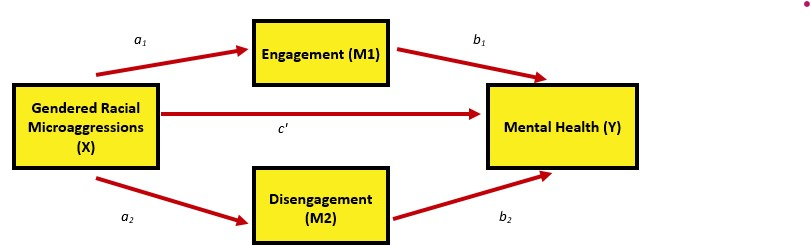
\includegraphics{images/CompMed/LewisParaMed.jpg}
\caption{An image of the parallel mediation we will work}
\end{figure}

We can use the guidelines above to specify our model and then request summaries of the fit indices and parameter estimates.

\begin{Shaded}
\begin{Highlighting}[]
\NormalTok{parallel\_Lewis }\OtherTok{\textless{}{-}} \StringTok{"}
\StringTok{    MntlHlth \textasciitilde{} b1*Engmt + b2*DisEngmt + c\_p*GRMS}
\StringTok{    Engmt \textasciitilde{} a1*GRMS    }
\StringTok{    DisEngmt \textasciitilde{} a2*GRMS}
\StringTok{    }
\StringTok{    indirect1 := a1 * b1}
\StringTok{    indirect2 := a2 * b2}
\StringTok{    contrast := indirect1 {-} indirect2}
\StringTok{    total\_indirects := indirect1 + indirect2}
\StringTok{    total\_c := c\_p + (indirect1) + (indirect2)}
\StringTok{    direct := c\_p}
\StringTok{"}
\FunctionTok{set.seed}\NormalTok{(}\DecValTok{230925}\NormalTok{)  }\CommentTok{\#necessary for reproducible results because lavaan introduces randomness into the estimation process}
\NormalTok{para\_Lewis\_fit }\OtherTok{\textless{}{-}}\NormalTok{ lavaan}\SpecialCharTok{::}\FunctionTok{sem}\NormalTok{(parallel\_Lewis, }\AttributeTok{data =}\NormalTok{ Lewis\_df, }\AttributeTok{se =} \StringTok{"bootstrap"}\NormalTok{,}
    \AttributeTok{bootstrap =} \DecValTok{1000}\NormalTok{, }\AttributeTok{missing =} \StringTok{"fiml"}\NormalTok{)  }\CommentTok{\#holds the \textquotesingle{}whole\textquotesingle{} result}
\NormalTok{pLewis\_sum }\OtherTok{\textless{}{-}}\NormalTok{ lavaan}\SpecialCharTok{::}\FunctionTok{summary}\NormalTok{(para\_Lewis\_fit, }\AttributeTok{standardized =} \ConstantTok{TRUE}\NormalTok{, }\AttributeTok{rsq =}\NormalTok{ T,}
    \AttributeTok{fit =} \ConstantTok{TRUE}\NormalTok{, }\AttributeTok{ci =} \ConstantTok{TRUE}\NormalTok{)  }\CommentTok{\#today, we really only need the R{-}squared from here    }
\NormalTok{pLewis\_ParEsts }\OtherTok{\textless{}{-}}\NormalTok{ lavaan}\SpecialCharTok{::}\FunctionTok{parameterEstimates}\NormalTok{(para\_Lewis\_fit, }\AttributeTok{boot.ci.type =} \StringTok{"bca.simple"}\NormalTok{,}
    \AttributeTok{standardized =} \ConstantTok{TRUE}\NormalTok{)  }\CommentTok{\#provides our estimates, se, p values for all the elements we specified}

\NormalTok{pLewis\_sum}
\NormalTok{pLewis\_ParEsts}
\end{Highlighting}
\end{Shaded}

\hypertarget{table-and-figure}{%
\subsubsection{Table and Figure}\label{table-and-figure}}

To assist in table preparation, it is possible to export the results to a .csv file that can be manipulated in Excel, Microsoft Word, or other program to prepare an APA style table.

\begin{Shaded}
\begin{Highlighting}[]
\FunctionTok{write.csv}\NormalTok{(pLewis\_ParEsts, }\AttributeTok{file =} \StringTok{"pLewis\_ParEsts.csv"}\NormalTok{)}
\end{Highlighting}
\end{Shaded}

We can use the package \href{https://cjvanlissa.github.io/tidySEM/articles/Plotting_graphs.html}{tidySEM} to create a figure that includes the values on the path.

Here's what the base package gets us

\begin{Shaded}
\begin{Highlighting}[]
\CommentTok{\# only worked when I used the library to turn on all these pkgs}
\FunctionTok{library}\NormalTok{(lavaan)}
\FunctionTok{library}\NormalTok{(dplyr)}
\FunctionTok{library}\NormalTok{(ggplot2)}
\FunctionTok{library}\NormalTok{(tidySEM)}
\NormalTok{tidySEM}\SpecialCharTok{::}\FunctionTok{graph\_sem}\NormalTok{(}\AttributeTok{model =}\NormalTok{ para\_Lewis\_fit)}
\end{Highlighting}
\end{Shaded}

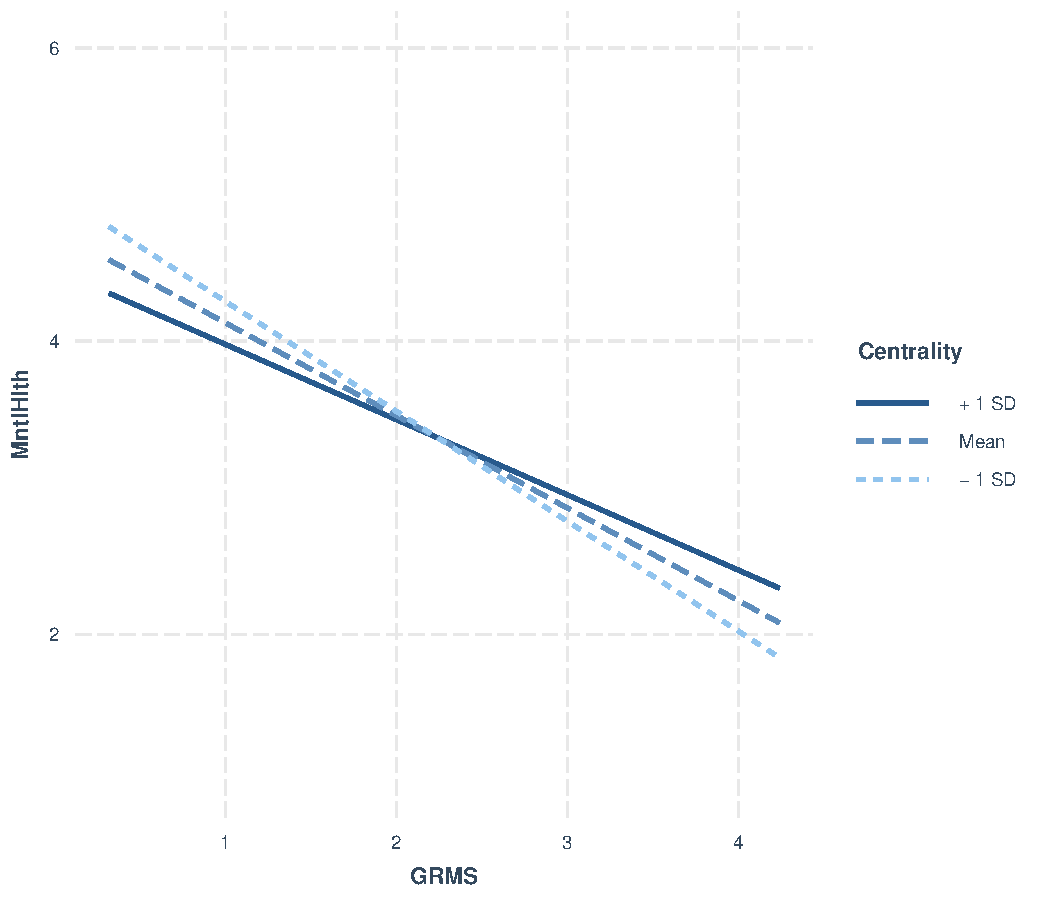
\includegraphics{06-ComplexMed_files/figure-latex/unnamed-chunk-20-1.pdf}

We can create model that communicates more intuitively with a little tinkering. First, let's retrieve the current ``map'' of the layout.

\begin{Shaded}
\begin{Highlighting}[]
\NormalTok{tidySEM}\SpecialCharTok{::}\FunctionTok{get\_layout}\NormalTok{(para\_Lewis\_fit)}
\end{Highlighting}
\end{Shaded}

\begin{verbatim}
##      [,1]    [,2]       [,3]      
## [1,] NA      "GRMS"     NA        
## [2,] "Engmt" "DisEngmt" "MntlHlth"
## attr(,"class")
## [1] "layout_matrix" "matrix"        "array"
\end{verbatim}

To create the figure I showed at the beginning of the chapter, we will want three rows and three columns.

\begin{Shaded}
\begin{Highlighting}[]
\NormalTok{pLewis\_map }\OtherTok{\textless{}{-}}\NormalTok{ tidySEM}\SpecialCharTok{::}\FunctionTok{get\_layout}\NormalTok{(}\StringTok{""}\NormalTok{, }\StringTok{"Engmt"}\NormalTok{, }\StringTok{""}\NormalTok{, }\StringTok{"GRMS"}\NormalTok{, }\StringTok{""}\NormalTok{, }\StringTok{"MntlHlth"}\NormalTok{,}
    \StringTok{""}\NormalTok{, }\StringTok{"DisEngmt"}\NormalTok{, }\StringTok{""}\NormalTok{, }\AttributeTok{rows =} \DecValTok{3}\NormalTok{)}
\NormalTok{pLewis\_map}
\end{Highlighting}
\end{Shaded}

\begin{verbatim}
##      [,1]   [,2]       [,3]      
## [1,] ""     "Engmt"    ""        
## [2,] "GRMS" ""         "MntlHlth"
## [3,] ""     "DisEngmt" ""        
## attr(,"class")
## [1] "layout_matrix" "matrix"        "array"
\end{verbatim}

We can update our figure by supplying this new map and adjusting the object and text sizes.

\begin{Shaded}
\begin{Highlighting}[]
\NormalTok{tidySEM}\SpecialCharTok{::}\FunctionTok{graph\_sem}\NormalTok{(para\_Lewis\_fit, }\AttributeTok{layout =}\NormalTok{ pLewis\_map, }\AttributeTok{rect\_width =} \FloatTok{1.5}\NormalTok{,}
    \AttributeTok{rect\_height =} \FloatTok{1.25}\NormalTok{, }\AttributeTok{spacing\_x =} \DecValTok{2}\NormalTok{, }\AttributeTok{spacing\_y =} \DecValTok{3}\NormalTok{, }\AttributeTok{text\_size =} \FloatTok{4.5}\NormalTok{)}
\end{Highlighting}
\end{Shaded}

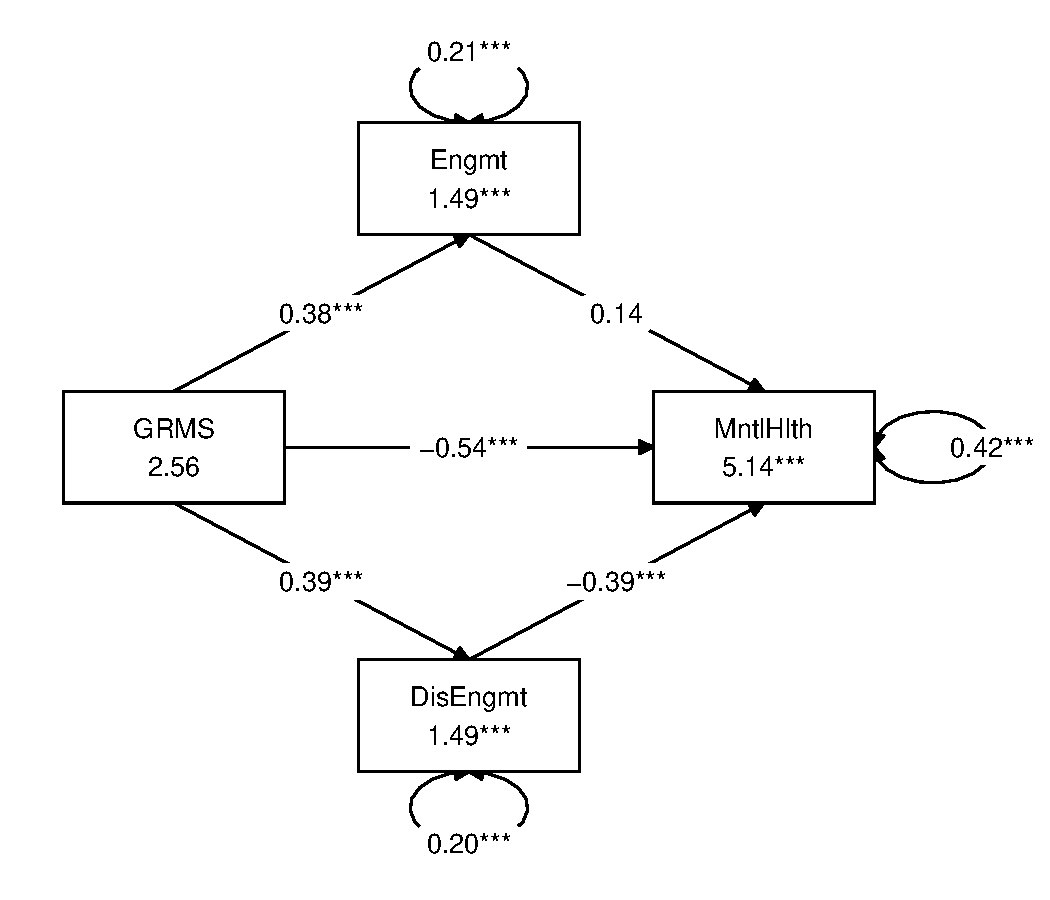
\includegraphics{06-ComplexMed_files/figure-latex/unnamed-chunk-23-1.pdf}

Now let's make a table.

\textbf{Table 2 }

\begin{longtable}[]{@{}
  >{\raggedright\arraybackslash}p{(\columnwidth - 0\tabcolsep) * \real{1.0000}}@{}}
\toprule\noalign{}
\begin{minipage}[b]{\linewidth}\raggedright
Model Coefficients Assessing Engagement and Disengagement Coping as Parallel Mediators Between Predicting Mental Health from Gendered Racial Microaggressions
\end{minipage} \\
\midrule\noalign{}
\endhead
\bottomrule\noalign{}
\endlastfoot
\end{longtable}

\begin{longtable}[]{@{}
  >{\raggedright\arraybackslash}p{(\columnwidth - 8\tabcolsep) * \real{0.4000}}
  >{\centering\arraybackslash}p{(\columnwidth - 8\tabcolsep) * \real{0.1286}}
  >{\centering\arraybackslash}p{(\columnwidth - 8\tabcolsep) * \real{0.1429}}
  >{\centering\arraybackslash}p{(\columnwidth - 8\tabcolsep) * \real{0.1143}}
  >{\centering\arraybackslash}p{(\columnwidth - 8\tabcolsep) * \real{0.2143}}@{}}
\toprule\noalign{}
\begin{minipage}[b]{\linewidth}\raggedright
Predictor
\end{minipage} & \begin{minipage}[b]{\linewidth}\centering
\(B\)
\end{minipage} & \begin{minipage}[b]{\linewidth}\centering
\(SE_{B}\)
\end{minipage} & \begin{minipage}[b]{\linewidth}\centering
\(p\)
\end{minipage} & \begin{minipage}[b]{\linewidth}\centering
\(R^2\)
\end{minipage} \\
\midrule\noalign{}
\endhead
\bottomrule\noalign{}
\endlastfoot
\end{longtable}

\begin{longtable}[]{@{}
  >{\raggedright\arraybackslash}p{(\columnwidth - 8\tabcolsep) * \real{0.4000}}
  >{\centering\arraybackslash}p{(\columnwidth - 8\tabcolsep) * \real{0.1286}}
  >{\centering\arraybackslash}p{(\columnwidth - 8\tabcolsep) * \real{0.1429}}
  >{\centering\arraybackslash}p{(\columnwidth - 8\tabcolsep) * \real{0.1143}}
  >{\centering\arraybackslash}p{(\columnwidth - 8\tabcolsep) * \real{0.2143}}@{}}
\toprule\noalign{}
\begin{minipage}[b]{\linewidth}\raggedright
Engagement coping (M1)
\end{minipage} & \begin{minipage}[b]{\linewidth}\centering
\end{minipage} & \begin{minipage}[b]{\linewidth}\centering
\end{minipage} & \begin{minipage}[b]{\linewidth}\centering
\end{minipage} & \begin{minipage}[b]{\linewidth}\centering
.27
\end{minipage} \\
\midrule\noalign{}
\endhead
\bottomrule\noalign{}
\endlastfoot
Constant & 1.494 & 0.111 & \textless0.001 & \\
GRMS (\(a_1\)) & 0.384 & 0.042 & \textless0.001 & \\
\end{longtable}

\begin{longtable}[]{@{}
  >{\raggedright\arraybackslash}p{(\columnwidth - 8\tabcolsep) * \real{0.4000}}
  >{\centering\arraybackslash}p{(\columnwidth - 8\tabcolsep) * \real{0.1286}}
  >{\centering\arraybackslash}p{(\columnwidth - 8\tabcolsep) * \real{0.1429}}
  >{\centering\arraybackslash}p{(\columnwidth - 8\tabcolsep) * \real{0.1143}}
  >{\centering\arraybackslash}p{(\columnwidth - 8\tabcolsep) * \real{0.2143}}@{}}
\toprule\noalign{}
\begin{minipage}[b]{\linewidth}\raggedright
Disengagement coping (M2)
\end{minipage} & \begin{minipage}[b]{\linewidth}\centering
\end{minipage} & \begin{minipage}[b]{\linewidth}\centering
\end{minipage} & \begin{minipage}[b]{\linewidth}\centering
\end{minipage} & \begin{minipage}[b]{\linewidth}\centering
.28
\end{minipage} \\
\midrule\noalign{}
\endhead
\bottomrule\noalign{}
\endlastfoot
Constant & 1.490 & 0.100 & \textless0.001 & \\
GRMS (\(a_2\)) & 0.386 & 0.038 & \textless0.001 & \\
\end{longtable}

\begin{longtable}[]{@{}
  >{\raggedright\arraybackslash}p{(\columnwidth - 8\tabcolsep) * \real{0.4000}}
  >{\centering\arraybackslash}p{(\columnwidth - 8\tabcolsep) * \real{0.1286}}
  >{\centering\arraybackslash}p{(\columnwidth - 8\tabcolsep) * \real{0.1429}}
  >{\centering\arraybackslash}p{(\columnwidth - 8\tabcolsep) * \real{0.1143}}
  >{\centering\arraybackslash}p{(\columnwidth - 8\tabcolsep) * \real{0.2143}}@{}}
\toprule\noalign{}
\begin{minipage}[b]{\linewidth}\raggedright
Mental Health (DV)
\end{minipage} & \begin{minipage}[b]{\linewidth}\centering
\end{minipage} & \begin{minipage}[b]{\linewidth}\centering
\end{minipage} & \begin{minipage}[b]{\linewidth}\centering
\end{minipage} & \begin{minipage}[b]{\linewidth}\centering
.37
\end{minipage} \\
\midrule\noalign{}
\endhead
\bottomrule\noalign{}
\endlastfoot
Constant & 5.141 & 0.226 & \textless0.001 & \\
Engagement (\(b_1\)) & 0.144 & 0.089 & 0.106 & \\
Disengagement (\(b_2\)) & -0.391 & 0.089 & \textless0.001 & \\
GRMS (\(c'\)) & -0.535 & 0.076 & \textless0.001 & \\
\end{longtable}

\begin{longtable}[]{@{}
  >{\raggedright\arraybackslash}p{(\columnwidth - 8\tabcolsep) * \real{0.4000}}
  >{\centering\arraybackslash}p{(\columnwidth - 8\tabcolsep) * \real{0.1286}}
  >{\centering\arraybackslash}p{(\columnwidth - 8\tabcolsep) * \real{0.1429}}
  >{\centering\arraybackslash}p{(\columnwidth - 8\tabcolsep) * \real{0.1143}}
  >{\centering\arraybackslash}p{(\columnwidth - 8\tabcolsep) * \real{0.2143}}@{}}
\toprule\noalign{}
\begin{minipage}[b]{\linewidth}\raggedright
Summary of Effects
\end{minipage} & \begin{minipage}[b]{\linewidth}\centering
\(B\)
\end{minipage} & \begin{minipage}[b]{\linewidth}\centering
\(SE_{B}\)
\end{minipage} & \begin{minipage}[b]{\linewidth}\centering
\(p\)
\end{minipage} & \begin{minipage}[b]{\linewidth}\centering
95\% CI
\end{minipage} \\
\midrule\noalign{}
\endhead
\bottomrule\noalign{}
\endlastfoot
Total & -0.631 & 0.058 & \textless0.001 & -0.739, -0.505 \\
Indirect 1 (\(a_1\) * \(a_2\)) & 0.055 & 0.036 & 0.121 & -0.003, 0.140 \\
Indirect 2 (\(b_1\) * \(b_2\)) & -0.151 & 0.038 & \textless0.001 & -0.235, -0.085 \\
Total indirects & -0.096 & 0.051 & 0.059 & -0.193, 0.007 \\
Contrast (Ind1 - Ind2) & 0.206 & 0.054 & \textless0.001 & 0.109, 0.338 \\
\end{longtable}

\begin{longtable}[]{@{}
  >{\raggedright\arraybackslash}p{(\columnwidth - 0\tabcolsep) * \real{1.0000}}@{}}
\toprule\noalign{}
\endhead
\bottomrule\noalign{}
\endlastfoot
\emph{Note}. GRMS = gendered racial microaggressions. The significance of the indirect effects was calculated with bootstrapped, bias-corrected, confidence intervals (.95). \\
\end{longtable}

\begin{itemize}
\tightlist
\item
  The model accounts for 37\% of the variance in predicting mental health outcomes.
\item
  The total effect of GRMS on mental health is -0.631 (\(p < 0.001\)) is negative and statistically significant. That is, gendered racial microaggressions have a statistically significant negative effect on mental health.
\item
  The direct effect of GRMS on mental health is -0.535 (\(p < 0.001\)); while this is lower than the total effect, it remains statistically significant.

  \begin{itemize}
  \tightlist
  \item
    Using Baron and Kenny's \citeyearpar{baron_moderator-mediator_1986} causal steps logic, the fact that the direct effect does not decrease in a statistically significant manner does not provide helpful, logical support for mediation. According to Hayes \citeyearpar{hayes_more_2022} this difference is not necessary. That is, a statistically significant indirect effect can stand on its own.
  \end{itemize}
\item
  Indirect effect \#1 (a1 x b1 or GRMS through engagement coping) is 0.055 (\(p = 0.121, CI95[-0.003, 0.140]\)) and not statistically significant. Because they can be inconsistent with the \emph{p} values, we should always check the confidence intervals to see if they pass through zero. In this case they do.
\item
  Indirect effect \#2 (a2 x b2, or GRMS through disengagement to coping) is -0.151 (\(p < 0.001, CI95[-0.235, -0.085]\)). The \emph{p} value is significant and the 95\% confidence interval does not pass through zero. Thus, gendered racial microaggressions lead to greater disengagement (\emph{a1}). In turn, disengagement has negative effects on mental health (\emph{b2}).
\item
  The total indirect effect (i.e., sum of all specific indirect effects) \((-0.096, p = 0.059)\) is not statistically significant.
\item
  We examine the contrast to see if the indirect effects statistically significantly different from each other: \(B= 0.206, p < 0.001\). They are. This is not surprising since the path mediated by engagement was not statistically significant but the path mediated by disengagement was statistically significant.
\end{itemize}

\hypertarget{apa-style-writeup-1}{%
\subsubsection{APA Style Writeup}\label{apa-style-writeup-1}}

Hayes \citep{hayes_introduction_2022} provides helpful guidelines for presenting statistical results. Here is a summary of his recommendations.

\begin{itemize}
\tightlist
\item
  Pack as much statistical info as possible into a table(s) or figure(s).
\item
  Use statistics in the text as punctuation; avoid redundancy in text and table.
\item
  Avoid using abbreviations for variables in the text itself; rather focus on the construct names rather than their shorthand
\item
  Avoid focusing on what you hypothesized (e.g., avoid, ``Results supported/did not support hypothesis A1'') and instead focus on what you found. The reader is more interested in the results, not your forecasts.
\item
  Hayes prefers reporting unstandardized metrics because they map onto the measurement scales used in the study. He believes this is especially important when dichotomous variables are used.
\item
  There is ``no harm'' in reporting hypothesis tests and CIs for the \emph{a} and \emph{b} paths, but whether/not these paths are statistically significant does not determine the significance of the indirect effect.
\item
  Be precise with language:
\item
  OK: X exerts an effect on Y directly and/or indirectly through M.
\item
  Not OK: the indirect effect of M\\
\item
  Report direct and indirect effects and their corresponding inferential tests
\item
  Hayes argues that a statistically significant indirect effect is, in fact statistic. He dislikes narration of the Baron and Kenny \citeyearpar{baron_moderator-mediator_1986} process and steps.
\end{itemize}

Here's my attempt to write up the simulated data from the Lewis et al. \citeyearpar{lewis_applying_2017} article.

\textbf{Method}

Data Analysis

Parallel multiple mediation is appropriate when testing the influence of an independent variable (X) on the dependent variable (Y) directly, as well as indirectly through two or more mediators. A condition of parallel multiple mediation is that no mediator causally influences another \citep{hayes_more_2022}. Using data simulated from Lewis et al. \citeyearpar{lewis_applying_2017} we utilized parallel multiple mediation analysis to test the influence of gendered racial microaggressions (X, GRMS) on mental health outcomes (Y, MntlHlth) directly as well as indirectly through the mediators engagement coping (M1, Engmt) and disengaged coping (M2, DisEngmt). Using the \emph{lavaan} (v. 0.6-16) package in R we followed the procedures outlined in Hayes \citeyearpar{hayes_more_2022} by analyzing the strength and significance of four sets of effects: specific indirect, the total indirect, the direct, and total.

\textbf{Results}

\textbf{Preliminary Analyses} Descriptive statistics were computed, and all variables were assessed for skewness and kurtosis. \emph{More narration,here.} A summary of descriptive statistics and a correlation matrix for the study is provided in Table 2. These bivariate relations provide evidence to support the test of mediation analysis.

\textbf{Parallel Multiple Mediation Analysis} A model of parallel mediation examined the degree to which engagement and disengagement coping strategies mediated the relation of gendered racial microaggressions on mental health outcomes in Black women. Hayes \citeyearpar{hayes_more_2022} recommended this strategy over simple mediation models because it allows for all mediators to be examined, simultaneously. The resultant direct and indirect values for each path account for other mediation paths. Using the \emph{lavaan} (v. 0.6-17) package in R, coefficients for specific indirect, total indirect, direct, and total were computed. Path coefficients refer to regression weights, or slopes, of the expected changes in the dependent variable given a unit change in the independent variables.

Results (depicted in Figure 2 and presented in Table 3) suggest that 37\% of the variance in mental health outcomes is accounted for by the model. The indirect effect predicting mental health from gendered racial microaggressions via engagement coping was not statistically significant \(*B = 0.055, SE = 0.036, p = 0.121, CI95[-0.003, 0.140 ]\)). Looking at the individual paths we see that \(a_{1}\) was positive and statistically significant (GRMS leds to increased engagement coping), but the subsequent link, \(b_{1}\) (engagement to mental health) was not. The indirect effect predicting mental health from gendered racial microaggressions through disengagement to coping was statistically significant \(B = -0.151, SE = 0.038, p < 0.001, CI95[-0.235, -0.085]\)). In this case, gendered racial microaggressions led to greater disengagement coping (\(a_{2}\)). In turn, disengagement coping had negative effects on mental health (\(b_{2}\)). Curiously, the total indirect effect (i.e., the sum of the specific indirect effects was not statistically significant. It is possible that the positive and negative valences of the indirect effects ``cancelled each other out.'' A pairwise comparison of the specific indirect effects indicated that the strength of the effects were statistically significantly different from each other. Given that the path through engagement coping was not significant, but the path through disengagement coping was, this statistically significant difference is not surprising.

\textbf{Hints for Writing Method/Results Sections}

\begin{itemize}
\tightlist
\item
  When you find an article you like, make note of it and put it in a very special folder. In recent years, I have learned to rely on full-text versions stored in my Zotero app.
\item
  Once you know your method (measure, statistic, etc.) begin collecting others articles that are similar to it. To write results sections I will often reference multiple articles.\\
\item
  When it iss time to write have all these resources handy and use them as guides/models.
\item
  Put as much info as possible in the table. Become a table-pro. That is, learn how to merge/split cells, use borders/shading, the decimal tab, and so forth. Don't make the borders disappear until the last thing you do before submitting. This is because you ALWAYS have to update your tables and seeing the borders makes it easier.
\end{itemize}

\hypertarget{serial-multiple-mediator-model}{%
\section{Serial Multiple Mediator Model}\label{serial-multiple-mediator-model}}

Recall that one of the conditions of the \emph{parallel mediator model} was that ``no mediator causally influences another.''

Regarding these correlated mediators \citep{hayes_more_2022}:

\begin{itemize}
\tightlist
\item
  Typically, two or more mediators that are causally located between X and Y will be correlated - if for no other reason than that they share a common cause (X).
\item
  Estimating the partial correlation between two mediators after controlling for X is one way to examine whether all of their association is accounted for by this common cause.
\item
  \emph{Partial correlation} is the Pearson correlation between the residuals from a model estimating Y from a set of covariates, and the residuals from a model estimating X from the same set of covariates.
\item
  Partial correlations allow the assessment of their association, independent of what they have in common with the covariates that were regressed onto Y and X, separately.
\item
  If two (or more) mediators remain correlated after adjusting for X, then
\item
  the correlation is \emph{spurious,} they share another (unmodeled) common cause.
\item
  the remaining association is \emph{epiphenomenal}. That is, a proposed mediator could be related to an outcome not because it causes the outcome, but because it is correlated with another variable that is causally influencing the outcome. This is a noncausal alternative explanation for an association. Also, many things correlated with the cause of Y will also tend to be correlated with X, but it doesn't make all those things cause Y
\item
  \emph{or one mediator causally affects another}
\end{itemize}

The goal of a serial multiple mediator model is to investigate the direct and indirect effects of X on Y while modeling a process in which X causes M1, which in turn causes M2, and so forth, concluding with Y as the final consequent.

As before, we will calculate:

\begin{itemize}
\tightlist
\item
  \emph{Direct effect, c':} the estimated difference in Y between two cases that differ by one unit on X but who are equal on all mediators in the model.
\item
  \emph{Specific indirect effects, a1b1, a2b2, a3b3, etc.:} constructed by multiplying the regression weights corresponding to each step in an indirect pathway; interpreted as the estimated difference in Y between two cases that differ by one unit on X through the causal sequence from X to mediator(s) to Y.
\item
  \emph{Total indirect effect of X:} sum of all specific indirect effects
\item
  \emph{Total effect of X:} the total indirect effect of X plus the direct effect of X; can also be estimated by regressing Y from X only.
\item
  \emph{Pairwise comparisons (contrasts) between indirect effects} (i.e., is one indirect effect stronger than another)
\end{itemize}

\hypertarget{we-stick-with-the-lewis-et-al.--lewis_applying_2017-example-but-modify-it.}{%
\subsection{\texorpdfstring{We stick with the Lewis et al. \citeyearpar{lewis_applying_2017} example, but modify it.}{We stick with the Lewis et al. {[}-@lewis\_applying\_2017{]} example, but modify it.}}\label{we-stick-with-the-lewis-et-al.--lewis_applying_2017-example-but-modify-it.}}

\begin{figure}
\centering
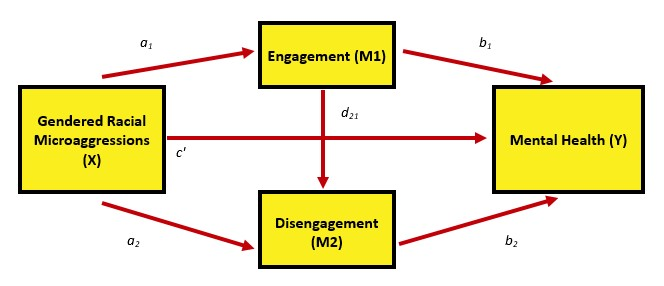
\includegraphics{images/CompMed/LewisSerialMed.jpg}
\caption{An image of the serial mediation we will work}
\end{figure}

Our parallel multiple mediator model of gendered racial microaggressions on mental health through engagement and disengagement coping strategies assumed no causal association between the mediators. Noting the statistically significant correlation between engagement and disengagement, what if engagement influenced disengagement, which, in turn influenced mental health.

If this is our goal (image), how many direct and indirect effects are contained in this model? Using the same processes as before, let's plan our model:

\begin{itemize}
\tightlist
\item
  We add a path predicting disengagement from engagement, and label it with a \(d_{21}\)

  \begin{itemize}
  \tightlist
  \item
    Regarding the notation, it makes sense that we use a \emph{d} to designate a new type of path; I don't know why we use a subscript of 21
  \end{itemize}
\item
  We specify a third indirect path that multiplies those 3 paths (a1, d21, b2) together
\item
  We add a third contrast so that we get all the combinations of indirect comparisons: 1-2, 1-3 2-3
\item
  We update our total\_indirects calculation to include indirect\#3
\item
  We update our total\_c calculation to include indirect\#3
\end{itemize}

\hypertarget{specify-the-lavaan-model}{%
\subsection{\texorpdfstring{Specify the \emph{lavaan} model}{Specify the lavaan model}}\label{specify-the-lavaan-model}}

\begin{Shaded}
\begin{Highlighting}[]
\NormalTok{serial\_Lewis }\OtherTok{\textless{}{-}} \StringTok{"}
\StringTok{    MntlHlth \textasciitilde{} b1*Engmt + b2*DisEngmt + c\_p*GRMS}
\StringTok{    Engmt \textasciitilde{} a1*GRMS    }
\StringTok{    DisEngmt \textasciitilde{} a2*GRMS}
\StringTok{    DisEngmt \textasciitilde{} d21*Engmt}
\StringTok{    }
\StringTok{    indirect1 := a1 * b1}
\StringTok{    indirect2 := a2 * b2}
\StringTok{    indirect3 := a1 * d21 * b2}
\StringTok{    contrast1 := indirect1 {-} indirect2}
\StringTok{    contrast2 := indirect1 {-} indirect3}
\StringTok{    contrast3 := indirect2 {-} indirect3}
\StringTok{    total\_indirects := indirect1 + indirect2 + indirect3}
\StringTok{    total\_c := c\_p + indirect1 + indirect2 + indirect3}
\StringTok{    direct := c\_p}
\StringTok{"}
\FunctionTok{set.seed}\NormalTok{(}\DecValTok{230925}\NormalTok{)  }\CommentTok{\#necessary for reproducible results because lavaan introduces randomness into the estimation process}
\NormalTok{serial\_Lewis\_fit }\OtherTok{\textless{}{-}}\NormalTok{ lavaan}\SpecialCharTok{::}\FunctionTok{sem}\NormalTok{(serial\_Lewis, }\AttributeTok{data =}\NormalTok{ Lewis\_df, }\AttributeTok{se =} \StringTok{"bootstrap"}\NormalTok{,}
    \AttributeTok{missing =} \StringTok{"fiml"}\NormalTok{, }\AttributeTok{bootstrap =} \DecValTok{1000}\NormalTok{)}
\NormalTok{sLewis\_sum }\OtherTok{\textless{}{-}}\NormalTok{ lavaan}\SpecialCharTok{::}\FunctionTok{summary}\NormalTok{(serial\_Lewis\_fit, }\AttributeTok{standardized =} \ConstantTok{TRUE}\NormalTok{, }\AttributeTok{rsq =}\NormalTok{ T,}
    \AttributeTok{fit =} \ConstantTok{TRUE}\NormalTok{, }\AttributeTok{ci =} \ConstantTok{TRUE}\NormalTok{)}
\NormalTok{sLewis\_ParEsts }\OtherTok{\textless{}{-}}\NormalTok{ lavaan}\SpecialCharTok{::}\FunctionTok{parameterEstimates}\NormalTok{(serial\_Lewis\_fit, }\AttributeTok{boot.ci.type =} \StringTok{"bca.simple"}\NormalTok{,}
    \AttributeTok{standardized =} \ConstantTok{TRUE}\NormalTok{)}

\NormalTok{sLewis\_sum}
\NormalTok{sLewis\_ParEsts}
\end{Highlighting}
\end{Shaded}

\hypertarget{table-and-figure-1}{%
\subsubsection{Table and Figure}\label{table-and-figure-1}}

To assist in table preparation, it is possible to export the results to a .csv file that can be manipulated in Excel, Microsoft Word, or other program to prepare an APA style table.

\begin{Shaded}
\begin{Highlighting}[]
\FunctionTok{write.csv}\NormalTok{(sLewis\_ParEsts, }\AttributeTok{file =} \StringTok{"sLewis\_ParEsts.csv"}\NormalTok{)}
\end{Highlighting}
\end{Shaded}

We can use the package \href{https://cjvanlissa.github.io/tidySEM/articles/Plotting_graphs.html}{tidySEM} to create a figure that includes the values on the path.

Here's what the base package gets us

\begin{Shaded}
\begin{Highlighting}[]
\CommentTok{\# only worked when I used the library to turn on all these pkgs}
\FunctionTok{library}\NormalTok{(lavaan)}
\FunctionTok{library}\NormalTok{(dplyr)}
\FunctionTok{library}\NormalTok{(ggplot2)}
\FunctionTok{library}\NormalTok{(tidySEM)}
\NormalTok{tidySEM}\SpecialCharTok{::}\FunctionTok{graph\_sem}\NormalTok{(}\AttributeTok{model =}\NormalTok{ serial\_Lewis\_fit)}
\end{Highlighting}
\end{Shaded}

\includegraphics{06-ComplexMed_files/figure-latex/unnamed-chunk-26-1.pdf}

We can create model that communicates more intuitively with a little tinkering. First, let's retrieve the current ``map'' of the layout.

\begin{Shaded}
\begin{Highlighting}[]
\NormalTok{tidySEM}\SpecialCharTok{::}\FunctionTok{get\_layout}\NormalTok{(serial\_Lewis\_fit)}
\end{Highlighting}
\end{Shaded}

\begin{verbatim}
##      [,1]    [,2]       [,3]      
## [1,] NA      "GRMS"     NA        
## [2,] "Engmt" "DisEngmt" "MntlHlth"
## attr(,"class")
## [1] "layout_matrix" "matrix"        "array"
\end{verbatim}

To create the figure I showed at the beginning of the chapter, we will want three rows and three columns.

\begin{Shaded}
\begin{Highlighting}[]
\NormalTok{sLewis\_map }\OtherTok{\textless{}{-}}\NormalTok{ tidySEM}\SpecialCharTok{::}\FunctionTok{get\_layout}\NormalTok{(}\StringTok{""}\NormalTok{, }\StringTok{"Engmt"}\NormalTok{, }\StringTok{""}\NormalTok{, }\StringTok{"GRMS"}\NormalTok{, }\StringTok{""}\NormalTok{, }\StringTok{"MntlHlth"}\NormalTok{,}
    \StringTok{""}\NormalTok{, }\StringTok{"DisEngmt"}\NormalTok{, }\StringTok{""}\NormalTok{, }\AttributeTok{rows =} \DecValTok{3}\NormalTok{)}
\NormalTok{sLewis\_map}
\end{Highlighting}
\end{Shaded}

\begin{verbatim}
##      [,1]   [,2]       [,3]      
## [1,] ""     "Engmt"    ""        
## [2,] "GRMS" ""         "MntlHlth"
## [3,] ""     "DisEngmt" ""        
## attr(,"class")
## [1] "layout_matrix" "matrix"        "array"
\end{verbatim}

We can update our figure by supplying this new map and adjusting the object and text sizes.

\begin{Shaded}
\begin{Highlighting}[]
\NormalTok{tidySEM}\SpecialCharTok{::}\FunctionTok{graph\_sem}\NormalTok{(serial\_Lewis\_fit, }\AttributeTok{layout =}\NormalTok{ sLewis\_map, }\AttributeTok{rect\_width =} \FloatTok{1.5}\NormalTok{,}
    \AttributeTok{rect\_height =} \FloatTok{1.25}\NormalTok{, }\AttributeTok{spacing\_x =} \DecValTok{2}\NormalTok{, }\AttributeTok{spacing\_y =} \DecValTok{3}\NormalTok{, }\AttributeTok{text\_size =} \FloatTok{4.5}\NormalTok{)}
\end{Highlighting}
\end{Shaded}

\includegraphics{06-ComplexMed_files/figure-latex/unnamed-chunk-29-1.pdf}

Now let's make a table.

\textbf{Table 4 }

\begin{longtable}[]{@{}
  >{\raggedright\arraybackslash}p{(\columnwidth - 0\tabcolsep) * \real{1.0000}}@{}}
\toprule\noalign{}
\begin{minipage}[b]{\linewidth}\raggedright
Model Coefficients Assessing Engagement and Disengagement Coping in a Model of Serial Mediation Predicting Mental Health from Gendered Racial Microaggressions
\end{minipage} \\
\midrule\noalign{}
\endhead
\bottomrule\noalign{}
\endlastfoot
\end{longtable}

\begin{longtable}[]{@{}
  >{\raggedright\arraybackslash}p{(\columnwidth - 8\tabcolsep) * \real{0.4000}}
  >{\centering\arraybackslash}p{(\columnwidth - 8\tabcolsep) * \real{0.1286}}
  >{\centering\arraybackslash}p{(\columnwidth - 8\tabcolsep) * \real{0.1429}}
  >{\centering\arraybackslash}p{(\columnwidth - 8\tabcolsep) * \real{0.1143}}
  >{\centering\arraybackslash}p{(\columnwidth - 8\tabcolsep) * \real{0.2143}}@{}}
\toprule\noalign{}
\begin{minipage}[b]{\linewidth}\raggedright
Predictor
\end{minipage} & \begin{minipage}[b]{\linewidth}\centering
\(B\)
\end{minipage} & \begin{minipage}[b]{\linewidth}\centering
\(SE_{B}\)
\end{minipage} & \begin{minipage}[b]{\linewidth}\centering
\(p\)
\end{minipage} & \begin{minipage}[b]{\linewidth}\centering
\(R^2\)
\end{minipage} \\
\midrule\noalign{}
\endhead
\bottomrule\noalign{}
\endlastfoot
\end{longtable}

\begin{longtable}[]{@{}
  >{\raggedright\arraybackslash}p{(\columnwidth - 8\tabcolsep) * \real{0.4000}}
  >{\centering\arraybackslash}p{(\columnwidth - 8\tabcolsep) * \real{0.1286}}
  >{\centering\arraybackslash}p{(\columnwidth - 8\tabcolsep) * \real{0.1429}}
  >{\centering\arraybackslash}p{(\columnwidth - 8\tabcolsep) * \real{0.1143}}
  >{\centering\arraybackslash}p{(\columnwidth - 8\tabcolsep) * \real{0.2143}}@{}}
\toprule\noalign{}
\begin{minipage}[b]{\linewidth}\raggedright
Engagement coping (M1)
\end{minipage} & \begin{minipage}[b]{\linewidth}\centering
\end{minipage} & \begin{minipage}[b]{\linewidth}\centering
\end{minipage} & \begin{minipage}[b]{\linewidth}\centering
\end{minipage} & \begin{minipage}[b]{\linewidth}\centering
.27
\end{minipage} \\
\midrule\noalign{}
\endhead
\bottomrule\noalign{}
\endlastfoot
Constant & 1.494 & 0.111 & \textless0.001 & \\
GRMS (\(a_1\)) & 0.384 & 0.042 & \textless0.001 & \\
\end{longtable}

\begin{longtable}[]{@{}
  >{\raggedright\arraybackslash}p{(\columnwidth - 8\tabcolsep) * \real{0.4000}}
  >{\centering\arraybackslash}p{(\columnwidth - 8\tabcolsep) * \real{0.1286}}
  >{\centering\arraybackslash}p{(\columnwidth - 8\tabcolsep) * \real{0.1429}}
  >{\centering\arraybackslash}p{(\columnwidth - 8\tabcolsep) * \real{0.1143}}
  >{\centering\arraybackslash}p{(\columnwidth - 8\tabcolsep) * \real{0.2143}}@{}}
\toprule\noalign{}
\begin{minipage}[b]{\linewidth}\raggedright
Disengagement coping (M2)
\end{minipage} & \begin{minipage}[b]{\linewidth}\centering
\end{minipage} & \begin{minipage}[b]{\linewidth}\centering
\end{minipage} & \begin{minipage}[b]{\linewidth}\centering
\end{minipage} & \begin{minipage}[b]{\linewidth}\centering
.29
\end{minipage} \\
\midrule\noalign{}
\endhead
\bottomrule\noalign{}
\endlastfoot
Constant & 1.400 & 0.128 & \textless0.001 & \\
GRMS (\(a_2\)) & 0.363 & 0.046 & \textless0.001 & \\
Engagement (\(d_{21}\)) & 0.061 & 0.059 & 0.304 & \\
\end{longtable}

\begin{longtable}[]{@{}
  >{\raggedright\arraybackslash}p{(\columnwidth - 8\tabcolsep) * \real{0.4000}}
  >{\centering\arraybackslash}p{(\columnwidth - 8\tabcolsep) * \real{0.1286}}
  >{\centering\arraybackslash}p{(\columnwidth - 8\tabcolsep) * \real{0.1429}}
  >{\centering\arraybackslash}p{(\columnwidth - 8\tabcolsep) * \real{0.1143}}
  >{\centering\arraybackslash}p{(\columnwidth - 8\tabcolsep) * \real{0.2143}}@{}}
\toprule\noalign{}
\begin{minipage}[b]{\linewidth}\raggedright
Mental Health (DV)
\end{minipage} & \begin{minipage}[b]{\linewidth}\centering
\end{minipage} & \begin{minipage}[b]{\linewidth}\centering
\end{minipage} & \begin{minipage}[b]{\linewidth}\centering
\end{minipage} & \begin{minipage}[b]{\linewidth}\centering
.37
\end{minipage} \\
\midrule\noalign{}
\endhead
\bottomrule\noalign{}
\endlastfoot
Constant & 5.141 & 0.226 & \textless0.001 & \\
Engagement (\(b_1\)) & 0.144 & 0.089 & 0.106 & \\
Disengagement (\(b_2\)) & -0.391 & 0.089 & \textless0.001 & \\
GRMS (\(c'\)) & -0.535 & 0.076 & \textless0.001 & \\
\end{longtable}

\begin{longtable}[]{@{}
  >{\raggedright\arraybackslash}p{(\columnwidth - 8\tabcolsep) * \real{0.4000}}
  >{\centering\arraybackslash}p{(\columnwidth - 8\tabcolsep) * \real{0.1286}}
  >{\centering\arraybackslash}p{(\columnwidth - 8\tabcolsep) * \real{0.1429}}
  >{\centering\arraybackslash}p{(\columnwidth - 8\tabcolsep) * \real{0.1143}}
  >{\centering\arraybackslash}p{(\columnwidth - 8\tabcolsep) * \real{0.2143}}@{}}
\toprule\noalign{}
\begin{minipage}[b]{\linewidth}\raggedright
Effects
\end{minipage} & \begin{minipage}[b]{\linewidth}\centering
\(B\)
\end{minipage} & \begin{minipage}[b]{\linewidth}\centering
\(SE_{B}\)
\end{minipage} & \begin{minipage}[b]{\linewidth}\centering
\(p\)
\end{minipage} & \begin{minipage}[b]{\linewidth}\centering
95\% CI
\end{minipage} \\
\midrule\noalign{}
\endhead
\bottomrule\noalign{}
\endlastfoot
Total effect & -0.631 & 0.059 & \textless0.001 & -0.739, -0.505 \\
Indirect 1 (\(a_1\) * \(a_2\)) & 0.055 & 0.036 & 0.121 & -0.003, 0.140 \\
Indirect 2 (\(b_1\) * \(b_2\)) & -0.142 & 0.038 & \textless0.001 & -0.227, -0.078 \\
Indirect 3 (\(b_1\) * \(d_{21}\) * \(b_2\)) & -0.009 & 0.009 & 0.339 & -0.032, 0.007 \\
Total indirects & -0.096 & 0.051 & 0.059 & -0.193, 0.007 \\
Contrast1 (Ind1 - Ind2) & 0.197 & 0.053 & \textless0.001 & 0.106, 0.318 \\
Contrast2 (Ind1 - Ind3) & 0.064 & 0.039 & 0.095 & 0.002, 0.156 \\
Contrast3 (Ind2 - Ind3) & -0.133 & 0.039 & 0.001 & -0.230, -0.066 \\
\end{longtable}

\begin{longtable}[]{@{}
  >{\raggedright\arraybackslash}p{(\columnwidth - 0\tabcolsep) * \real{1.0000}}@{}}
\toprule\noalign{}
\endhead
\bottomrule\noalign{}
\endlastfoot
\emph{Note}. GRMS = gendered racial microaggressions. The significance of the indirect effects was calculated with bootstrapped, bias-corrected, confidence intervals (.95). \\
\end{longtable}

Working through the data, we should be able to find these items:

\begin{itemize}
\tightlist
\item
  The model accounts for 37\% of the variance in predicting mental health outcomes.
\item
  The total effect of GRMS (X) on mental health (Y) is \(-0.631, (p < .001)\); it is negative and statistically significant.
\item
  The direct effect of GRMS (X) on mental health (Y) (\(-0.535, p < 0.001\)) is still negative. Although someone lower in magnitute, it is still statistically significant. While inconsistent with the Baron and Kenny \citeyearpar{baron_moderator-mediator_1986} logic of mediation, Hayes \citep{hayes_more_2022} argues that a statistically significant indirect effect can stand on its own.
\item
  Indirect effect \#1 (\(a_{1}\) x \(b_{1}\) or GRMS through engagement coping to mental health) is \(B = 0.055, p =0.121\). As in the parallel mediation, \(p\) is \textgreater{} .05 and the 95\% CIs pass through zero \((-0.003, 0.140)\). Examining the individual paths, there is a statistically significant relationship from GRMS to engagement, but not from engagement to mental health.
\item
  Indirect effect \#2 (\(a_{2}\) x \(b_{2}\), or GRMS through disengagement coping to mental health, is \(B = -0.142, p < 0.001, 95CI (-0.227, -0.078)\). Each of the paths is statistically significant from zero and so is the indirect effect.
\item
  Indirect effect \#3 (\(a_{2}\) x \(d_{21}\) x \(b_{2}\); GRMS through engagement coping through disengagement coping to mental health) is \(B = -0.009, p = 0.339, 95CI (-0.032, 0.007)\). This indirect effect involves \(a_{1}\) (GRMS to engagement) and \(b_{2}\) which are significant. However, the path from engagement coping to disengagement coping is not significant.
\item
  Total indirect: \(B = -0.096, p = 0.059\) is the sum of all specific indirect effects and is not statistically significant. The positive and negative indirects likely cancel each other out.
\item
  With \textbf{contrasts} we ask: Are the indirect effects statistically significantly different from each other?

  \begin{itemize}
  \tightlist
  \item
    Contrast 1 (indirect 1 v 2): \(B = 0.197, p <0.001)\), yes
  \item
    Contrast 2 (indirect 1 v 3): \(B = 0.064, p = 0.095\), no
  \item
    Contrast 3 (indirect 2 v 3): \(B = -0.133,p = 0.001p\), yes
  \item
    This formal test of contrasts is an important one. It is not ok to infer that effects are statistically significantly different than each other on the basis of their estimates or \(p\) values. The formal test allows us to claim (with justification) that there are statistically significant differences between indirect effects 1 and 2; and 2 and 3.
  \end{itemize}
\end{itemize}

\hypertarget{apa-style-writeup-2}{%
\subsection{APA Style Writeup}\label{apa-style-writeup-2}}

\textbf{Method}

\textbf{Data Analysis} Serial multiple mediation is appropriate when testing the influence of an independent variable (X) on the dependent variable (Y) directly, as well as indirectly through two or more mediators (M) and there is reason to hypothesize that variables that are causally prior in the model affect all variables later in the causal sequence \citep{hayes_more_2022}. We utilized serial multiple mediation analysis to test the influence of gendered racial microaggressions (X, GRMS) on mental health (Y, MntlHlth) directly as well as indirectly through the mediators engagement coping (M1, Engmt) and disengagement coping (M2, DisEngmt). Moreover, we hypothesized a causal linkage between from the engagement coping mediator to the disengagement coping mediator such that a third specific indirect effect began with GRMS (X) through engagement coping (M1) through disengagement coping (M2) to mental health (Y). Using the \emph{lavaan} (v. 0.6-16) package in R we followed the procedures outlined in Hayes \citeyearpar{hayes_more_2022} by analyzing the strength and significance of four sets of effects: specific indirect, the total indirect, the direct, and total. Bootstrap analysis, a nonparametric sampling procedure, was used to test the significance of the indirect effects.

\emph{Hayes would likely recommend that we say this with fewer acronyms and more words/story.}

\textbf{Results} \textbf{Preliminary Analyses} Descriptive statistics were computed, and all variables were assessed univariate normality. \emph{You would give your results regarding skew, kurtosis, Shapiro Wilks', here. If relevant, you could also describe multivariate normality.} A summary of descriptive statistics and a correlation matrix for the study is provided in Table 1. These bivariate relations provide evidence to support the test of mediation analysis.

\textbf{Serial Multiple Mediation Analysis} A model of serial multiple mediation was analyzed examining the degree to which engagement and disengagement coping mediated the relationship between gendered racial microaggressions and mental health outcomes. Hayes \citeyearpar{hayes_more_2022} recommended this strategy over simple mediation models because it allows for all mediators to be examined, simultaneously and allows the testing of the seriated effect of prior mediators onto subsequent ones. Using the \emph{lavaan} (v. 0.6-16) package in R, coefficients for specific indirect, total indirect, direct, and total were computed. Path coefficients refer to regression weights, or slopes, of the expected changes in the dependent variable given a unit change in the independent variables.

Results (depicted in Figure \# and presented in Table \#) suggest that 37\% of the variance in behavioral intentions is accounted for by the three variables in the model. Two of the specific indirect effects were significant and were statistically significantly different from each other. Specifically, the effect of gendered racial microaggressions through disengagement coping to mental health (\(B= -0.142, SE = 0.038, p < .001, 95CI[-0.227, -0.078]\)) was stronger than the indirect effect from gendered racial microaggressions through engagement coping through disengagement coping to mental health (\(B = 0.055, SE = 0.036, p =0.121, 95CI [-0.003, 0.140]\)). Interpreting the results suggests that, mental health outcomes are negatively impacted by gendered racial microaggressions direct and indirectly through disengagement coping. It is this latter path that has the greatest impact.

\emph{Note}: In a manner consistent with the Lewis et al. \citeyearpar{lewis_applying_2017} article, the APA Results section can be fairly short. This is especially true when a well-organized table presents the results. In fact, I oculd have left all the numbers out of this except for the \(R^2\) (because it was not reported in the table).

\hypertarget{stay-tuned-1}{%
\section{STAY TUNED}\label{stay-tuned-1}}

A section on power analysis is planned and coming soon! My apologies that it's not quite \emph{R}eady.

\hypertarget{troubleshooting-and-faqs}{%
\section{Troubleshooting and FAQs}\label{troubleshooting-and-faqs}}

An indirect effect that was (seemingly) significant in a simple (single) mediation disappears when additional mediators are added.

\begin{itemize}
\tightlist
\item
  Correlated mediators (e.g., multicollinearity) is a likely possibility.
\item
  Which is correct? Maybe both\ldots{}
\end{itemize}

A total effect was not significant, but there is one or more statistically significant specific indirect effect

\begin{itemize}
\tightlist
\item
  Recall that a total effect equals the sum of direct and indirect effects. If one specific indirect effect is positive and another is negative, this could account for the NS total effect.
\item
  If the direct effect is NS, but the indirect effects are significant, this might render the total effect NS.
\item
  The indirect effects might operate differently in subpopulations (males, females).
\end{itemize}

Your editor/peer reviewer/dissertation chair-or-committee member may insist that you do this the Baron \& Kenny way (aka ``the causal steps approach'').

\begin{itemize}
\tightlist
\item
  Hayes \citep{hayes_introduction_2022} provides compelling arguments for how to justify your (I believe correct) decision to just use the PROCESS (aka, bootstrapped, bias corrected, CIs )approach.
\item
  My favorite line in his text reads, '' (the Baron and Kenny way)\ldots is still being taught and recommended by researchers who don't follow the methodology literature.''
\end{itemize}

How can I extend a mediation (only) model to include multiple Xs, Ys, or COVs?

\begin{itemize}
\tightlist
\item
  There is fabulous, fabulous narration and syntax for doing all of this in Hayes text. Of course his mechanics are in PROCESS, but \emph{lavaan} is easy to use by just ``drawing more paths'' via the syntax. We'll get more practice as we go along.
\end{itemize}

What about effect sizes? Shouldn't we be including/reporting them?

\begin{itemize}
\tightlist
\item
  Yes! The closest thing we have reported to an effect size is \(R^2\), which assess proportion of variance accounted for in the M and Y variables.\\
\item
  In PROCESS and path analysis this is still emerging. Hayes chapter 4 presents a handful of options for effect sizes beyond \(R^2\).
\end{itemize}

\hypertarget{practice-problems-5}{%
\section{Practice Problems}\label{practice-problems-5}}

The three problems described below are designed to be grow in this series of chapters that begins with simple mediation and progresses through complex mediation, moderated moderation, and conditional process analysis. The goal of this assignment is to conduct a complex (e.g., parallel or serial) mediation.

I recommend that you select a dataset that includes at least four variables. If you are new to this topic, you may wish to select variables that are all continuously scaled. The IV and moderator (in subsequent chapters) \emph{could} be categorical (if they are dichotomous, please use 0/1 coding; if they have more than one category it is best if they are ordered). You will likely encounter challenges that were not covered in this chapter. Search for and try out solutions, knowing that there are multiple paths through the analysis.

The suggested practice problem for this chapter is to conduct a parallel or serial mediation (or both).

\hypertarget{problem-1-rework-the-research-vignette-as-demonstrated-but-change-the-random-seed-1}{%
\subsection{Problem \#1: Rework the research vignette as demonstrated, but change the random seed}\label{problem-1-rework-the-research-vignette-as-demonstrated-but-change-the-random-seed-1}}

If conducting a parallel or serial mediation feels a bit overwhelming, simply change the random seed in the data simulation, then rework one of the chapter problems (i.e., parallel or serial mediation). This should provide minor changes to the data (maybe in the second or third decimal point), but the results will likely be very similar.

\hypertarget{problem-2-rework-the-research-vignette-but-swap-one-or-more-variables-1}{%
\subsection{Problem \#2: Rework the research vignette, but swap one or more variables}\label{problem-2-rework-the-research-vignette-but-swap-one-or-more-variables-1}}

Conduct the complex mediation (parallel or serial) using the simulated data provided in this chapter, but swap out one or more of the variables. This could mean changing roles for the variables that were the focus of the chapter, or substituting one or more variables for those in the simulated data but not modeled in the chapter.

\hypertarget{problem-3-use-other-data-that-is-available-to-you-1}{%
\subsection{Problem \#3: Use other data that is available to you}\label{problem-3-use-other-data-that-is-available-to-you-1}}

To conduct the parallel or serial mediation, use data for which you have permission and access. This could be IRB approved data you have collected or from your lab; data you simulate from a published article; data from an open science repository; or data from other chapters (or the ``homeworked example'') in this OER.

\hypertarget{grading-rubric-5}{%
\subsection{Grading Rubric}\label{grading-rubric-5}}

\begin{longtable}[]{@{}
  >{\raggedright\arraybackslash}p{(\columnwidth - 4\tabcolsep) * \real{0.7642}}
  >{\centering\arraybackslash}p{(\columnwidth - 4\tabcolsep) * \real{0.1220}}
  >{\centering\arraybackslash}p{(\columnwidth - 4\tabcolsep) * \real{0.1138}}@{}}
\toprule\noalign{}
\begin{minipage}[b]{\linewidth}\raggedright
Assignment Component
\end{minipage} & \begin{minipage}[b]{\linewidth}\centering
\end{minipage} & \begin{minipage}[b]{\linewidth}\centering
\end{minipage} \\
\midrule\noalign{}
\endhead
\bottomrule\noalign{}
\endlastfoot
1. Assign each variable to the X, Y, M1, and M2 roles & 5 & \_\_\_\_\_ \\
4. Use tidySEM to create a figure that represents your results & 5 & \_\_\_\_\_ \\
5. Create a table that includes a summary of the effects (indirect, direct, total, total indirect) as well as contrasts & 5 & \_\_\_\_\_ \\
6. Represent your work in an APA-style write-up & 5 & \_\_\_\_\_ \\
7. Explanation to grader & 5 & \_\_\_\_\_ \\
8. Be able to hand-calculate the indirect, direct, and total effects from the a, b, \& c' paths & 5 & \_\_\_\_\_ \\
\textbf{Totals} & 40 & \_\_\_\_\_ \\
\end{longtable}

\hypertarget{homeworked-example-3}{%
\section{Homeworked Example}\label{homeworked-example-3}}

\href{https://youtu.be/p-iScWS_tT0}{Screencast Link}

For more information about the data used in this homeworked example, please refer to the description and codebook located at the end of the \href{https://lhbikos.github.io/ReCenterPsychStats/ReCintro.html\#introduction-to-the-data-set-used-for-homeworked-examples}{introductory lesson} in \href{https://lhbikos.github.io/ReCenterPsychStats/}{ReCentering Psych Stats}. An .rds file which holds the data is located in the \href{https://github.com/lhbikos/ReC_MultivModel/tree/main/Worked_Examples}{Worked Examples} folder at the GitHub site the hosts the OER. The file name is \emph{ReC.rds}.

The suggested practice problem for this chapter is to conduct a complex (i.e., parallel or serial) mediation.

\hypertarget{assign-each-variable-to-the-x-y-m1-and-m2-roles}{%
\subsection*{Assign each variable to the X, Y, M1, and M2 roles}\label{assign-each-variable-to-the-x-y-m1-and-m2-roles}}


X = Centering: explicit recentering (0 = precentered; 1 = recentered) M1 = TradPed: traditional pedagogy (continuously scaled with higher scores being more favorable) M2 = SRPed: socially responsive pedagogy (continuously scaled with higher scores being more favorable) Y = Valued: valued by me (continuously scaled with higher scores being more favorable)

In this \emph{parallel mediation}, I am hypothesizing that the perceived course value to the students is predicted by intentional recentering through their assessments of traditional and socially responsive pedagogy.

It helps me to make a quick sketch:

\begin{figure}
\centering
\includegraphics{Worked_Examples/images/CompMedHWfig.jpg}
\caption{An image of the parallel mediation model for the homeworked example.}
\end{figure}

\hypertarget{import-the-data-and-format-the-variables-in-the-model-1}{%
\subsection*{Import the data and format the variables in the model}\label{import-the-data-and-format-the-variables-in-the-model-1}}


\begin{Shaded}
\begin{Highlighting}[]
\NormalTok{raw }\OtherTok{\textless{}{-}} \FunctionTok{readRDS}\NormalTok{(}\StringTok{"ReC.rds"}\NormalTok{)}
\end{Highlighting}
\end{Shaded}

The approach we are taking to complex mediation does not allow dependency in the data. Therefore, we will include only those who took the multivariate class (i.e., excluding responses for the ANOVA and psychometrics courses).

\begin{Shaded}
\begin{Highlighting}[]
\NormalTok{raw }\OtherTok{\textless{}{-}}\NormalTok{ (dplyr}\SpecialCharTok{::}\FunctionTok{filter}\NormalTok{(raw, Course }\SpecialCharTok{==} \StringTok{"Multivariate"}\NormalTok{))}
\end{Highlighting}
\end{Shaded}

I need to score the TradPed, SRPed, and Valued variables

\begin{Shaded}
\begin{Highlighting}[]
\NormalTok{TradPed\_vars }\OtherTok{\textless{}{-}} \FunctionTok{c}\NormalTok{(}\StringTok{"ClearResponsibilities"}\NormalTok{, }\StringTok{"EffectiveAnswers"}\NormalTok{, }\StringTok{"Feedback"}\NormalTok{,}
    \StringTok{"ClearOrganization"}\NormalTok{, }\StringTok{"ClearPresentation"}\NormalTok{)}
\NormalTok{raw}\SpecialCharTok{$}\NormalTok{TradPed }\OtherTok{\textless{}{-}}\NormalTok{ sjstats}\SpecialCharTok{::}\FunctionTok{mean\_n}\NormalTok{(raw[, ..TradPed\_vars], }\FloatTok{0.75}\NormalTok{)}

\NormalTok{Valued\_vars }\OtherTok{\textless{}{-}} \FunctionTok{c}\NormalTok{(}\StringTok{"ValObjectives"}\NormalTok{, }\StringTok{"IncrUnderstanding"}\NormalTok{, }\StringTok{"IncrInterest"}\NormalTok{)}
\NormalTok{raw}\SpecialCharTok{$}\NormalTok{Valued }\OtherTok{\textless{}{-}}\NormalTok{ sjstats}\SpecialCharTok{::}\FunctionTok{mean\_n}\NormalTok{(raw[, ..Valued\_vars], }\FloatTok{0.75}\NormalTok{)}

\NormalTok{SRPed\_vars }\OtherTok{\textless{}{-}} \FunctionTok{c}\NormalTok{(}\StringTok{"InclusvClassrm"}\NormalTok{, }\StringTok{"EquitableEval"}\NormalTok{, }\StringTok{"MultPerspectives"}\NormalTok{,}
    \StringTok{"DEIintegration"}\NormalTok{)}
\NormalTok{raw}\SpecialCharTok{$}\NormalTok{SRPed }\OtherTok{\textless{}{-}}\NormalTok{ sjstats}\SpecialCharTok{::}\FunctionTok{mean\_n}\NormalTok{(raw[, ..SRPed\_vars], }\FloatTok{0.75}\NormalTok{)}
\end{Highlighting}
\end{Shaded}

I will create a babydf.

\begin{Shaded}
\begin{Highlighting}[]
\NormalTok{babydf }\OtherTok{\textless{}{-}}\NormalTok{ dplyr}\SpecialCharTok{::}\FunctionTok{select}\NormalTok{(raw, Centering, TradPed, Valued, SRPed)}
\end{Highlighting}
\end{Shaded}

Let's check the structure of the variables:

\begin{Shaded}
\begin{Highlighting}[]
\FunctionTok{str}\NormalTok{(babydf)}
\end{Highlighting}
\end{Shaded}

\begin{verbatim}
## Classes 'data.table' and 'data.frame':   84 obs. of  4 variables:
##  $ Centering: Factor w/ 2 levels "Pre","Re": 2 2 2 2 2 2 2 2 2 2 ...
##  $ TradPed  : num  3.8 5 4.8 4 4.2 3 5 4.6 4 4.8 ...
##  $ Valued   : num  4.33 5 4.67 3.33 4 3.67 5 4 4.67 4.67 ...
##  $ SRPed    : num  4.5 5 5 5 4.75 4.5 5 4.5 5 5 ...
##  - attr(*, ".internal.selfref")=<externalptr>
\end{verbatim}

At this point, these my only inclusion/exclusion criteria. I can determine how many students (who consented) completed any portion of the survey.

\hypertarget{specify-and-run-the-lavaan-model-1}{%
\subsection*{Specify and run the lavaan model}\label{specify-and-run-the-lavaan-model-1}}


\begin{Shaded}
\begin{Highlighting}[]
\NormalTok{ReCpMed }\OtherTok{\textless{}{-}} \StringTok{"}
\StringTok{          Valued \textasciitilde{} b1*TradPed + b2*SRPed + c\_p*Centering}
\StringTok{          TradPed \textasciitilde{} a1*Centering}
\StringTok{          SRPed \textasciitilde{} a2*Centering}
\StringTok{          }
\StringTok{          indirect1 := a1 * b1}
\StringTok{          indirect2 := a2 * b2}
\StringTok{          contrast := indirect1 {-} indirect2}
\StringTok{          total\_indirects := indirect1 + indirect2}
\StringTok{          total\_c    := c\_p + (indirect1) + (indirect2)}
\StringTok{          direct := c\_p}

\StringTok{          "}

\FunctionTok{set.seed}\NormalTok{(}\DecValTok{230916}\NormalTok{)  }\CommentTok{\#needed for reproducible results since lavaan includes randomness in its estimates}
\NormalTok{ReCpMedfit }\OtherTok{\textless{}{-}}\NormalTok{ lavaan}\SpecialCharTok{::}\FunctionTok{sem}\NormalTok{(ReCpMed, }\AttributeTok{data =}\NormalTok{ babydf, }\AttributeTok{se =} \StringTok{"bootstrap"}\NormalTok{, }\AttributeTok{missing =} \StringTok{"fiml"}\NormalTok{)}
\NormalTok{ReCpMedsummary }\OtherTok{\textless{}{-}}\NormalTok{ lavaan}\SpecialCharTok{::}\FunctionTok{summary}\NormalTok{(ReCpMedfit, }\AttributeTok{standardized =}\NormalTok{ T, }\AttributeTok{rsq =}\NormalTok{ T,}
    \AttributeTok{fit =} \ConstantTok{TRUE}\NormalTok{, }\AttributeTok{ci =} \ConstantTok{TRUE}\NormalTok{)}
\NormalTok{ReC\_pMedParamEsts }\OtherTok{\textless{}{-}}\NormalTok{ lavaan}\SpecialCharTok{::}\FunctionTok{parameterEstimates}\NormalTok{(ReCpMedfit, }\AttributeTok{boot.ci.type =} \StringTok{"bca.simple"}\NormalTok{,}
    \AttributeTok{standardized =} \ConstantTok{TRUE}\NormalTok{)}
\NormalTok{ReCpMedsummary}
\end{Highlighting}
\end{Shaded}

\begin{verbatim}
## lavaan 0.6.16 ended normally after 23 iterations
## 
##   Estimator                                         ML
##   Optimization method                           NLMINB
##   Number of model parameters                        11
## 
##   Number of observations                            84
##   Number of missing patterns                         3
## 
## Model Test User Model:
##                                                       
##   Test statistic                                54.059
##   Degrees of freedom                                 1
##   P-value (Chi-square)                           0.000
## 
## Model Test Baseline Model:
## 
##   Test statistic                               145.642
##   Degrees of freedom                                 6
##   P-value                                        0.000
## 
## User Model versus Baseline Model:
## 
##   Comparative Fit Index (CFI)                    0.620
##   Tucker-Lewis Index (TLI)                      -1.280
##                                                       
##   Robust Comparative Fit Index (CFI)             0.613
##   Robust Tucker-Lewis Index (TLI)               -1.323
## 
## Loglikelihood and Information Criteria:
## 
##   Loglikelihood user model (H0)               -202.536
##   Loglikelihood unrestricted model (H1)       -175.506
##                                                       
##   Akaike (AIC)                                 427.071
##   Bayesian (BIC)                               453.810
##   Sample-size adjusted Bayesian (SABIC)        419.110
## 
## Root Mean Square Error of Approximation:
## 
##   RMSEA                                          0.795
##   90 Percent confidence interval - lower         0.623
##   90 Percent confidence interval - upper         0.982
##   P-value H_0: RMSEA <= 0.050                    0.000
##   P-value H_0: RMSEA >= 0.080                    1.000
##                                                       
##   Robust RMSEA                                   0.815
##   90 Percent confidence interval - lower         0.641
##   90 Percent confidence interval - upper         1.004
##   P-value H_0: Robust RMSEA <= 0.050             0.000
##   P-value H_0: Robust RMSEA >= 0.080             1.000
## 
## Standardized Root Mean Square Residual:
## 
##   SRMR                                           0.217
## 
## Parameter Estimates:
## 
##   Standard errors                            Bootstrap
##   Number of requested bootstrap draws             1000
##   Number of successful bootstrap draws            1000
## 
## Regressions:
##                    Estimate  Std.Err  z-value  P(>|z|) ci.lower ci.upper
##   Valued ~                                                              
##     TradPed   (b1)    0.686    0.131    5.217    0.000    0.451    0.955
##     SRPed     (b2)    0.119    0.146    0.816    0.414   -0.193    0.400
##     Centerng (c_p)    0.015    0.103    0.143    0.886   -0.182    0.230
##   TradPed ~                                                             
##     Centerng  (a1)    0.312    0.137    2.283    0.022    0.047    0.582
##   SRPed ~                                                               
##     Centerng  (a2)    0.353    0.113    3.124    0.002    0.130    0.569
##    Std.lv  Std.all
##                   
##     0.686    0.747
##     0.119    0.104
##     0.015    0.011
##                   
##     0.312    0.210
##                   
##     0.353    0.296
## 
## Intercepts:
##                    Estimate  Std.Err  z-value  P(>|z|) ci.lower ci.upper
##    .Valued            0.710    0.469    1.514    0.130   -0.177    1.664
##    .TradPed           3.870    0.231   16.773    0.000    3.419    4.291
##    .SRPed             4.029    0.186   21.617    0.000    3.675    4.396
##    Std.lv  Std.all
##     0.710    1.077
##     3.870    5.396
##     4.029    7.013
## 
## Variances:
##                    Estimate  Std.Err  z-value  P(>|z|) ci.lower ci.upper
##    .Valued            0.181    0.027    6.658    0.000    0.118    0.224
##    .TradPed           0.492    0.128    3.837    0.000    0.259    0.733
##    .SRPed             0.301    0.060    5.007    0.000    0.193    0.425
##    Std.lv  Std.all
##     0.181    0.418
##     0.492    0.956
##     0.301    0.912
## 
## R-Square:
##                    Estimate
##     Valued            0.582
##     TradPed           0.044
##     SRPed             0.088
## 
## Defined Parameters:
##                    Estimate  Std.Err  z-value  P(>|z|) ci.lower ci.upper
##     indirect1         0.214    0.105    2.045    0.041    0.032    0.442
##     indirect2         0.042    0.053    0.790    0.429   -0.080    0.148
##     contrast          0.172    0.125    1.373    0.170   -0.024    0.469
##     total_indircts    0.256    0.109    2.346    0.019    0.051    0.469
##     total_c           0.271    0.142    1.914    0.056    0.003    0.576
##     direct            0.015    0.103    0.143    0.887   -0.182    0.230
##    Std.lv  Std.all
##     0.214    0.157
##     0.042    0.031
##     0.172    0.126
##     0.256    0.188
##     0.271    0.199
##     0.015    0.011
\end{verbatim}

\begin{Shaded}
\begin{Highlighting}[]
\NormalTok{ReC\_pMedParamEsts}
\end{Highlighting}
\end{Shaded}

\begin{verbatim}
##                lhs op                         rhs           label   est    se
## 1           Valued  ~                     TradPed              b1 0.686 0.131
## 2           Valued  ~                       SRPed              b2 0.119 0.146
## 3           Valued  ~                   Centering             c_p 0.015 0.103
## 4          TradPed  ~                   Centering              a1 0.312 0.137
## 5            SRPed  ~                   Centering              a2 0.353 0.113
## 6           Valued ~~                      Valued                 0.181 0.027
## 7          TradPed ~~                     TradPed                 0.492 0.128
## 8            SRPed ~~                       SRPed                 0.301 0.060
## 9        Centering ~~                   Centering                 0.233 0.000
## 10          Valued ~1                                             0.710 0.469
## 11         TradPed ~1                                             3.870 0.231
## 12           SRPed ~1                                             4.029 0.186
## 13       Centering ~1                                             1.369 0.000
## 14       indirect1 :=                       a1*b1       indirect1 0.214 0.105
## 15       indirect2 :=                       a2*b2       indirect2 0.042 0.053
## 16        contrast :=         indirect1-indirect2        contrast 0.172 0.125
## 17 total_indirects :=         indirect1+indirect2 total_indirects 0.256 0.109
## 18         total_c := c_p+(indirect1)+(indirect2)         total_c 0.271 0.142
## 19          direct :=                         c_p          direct 0.015 0.103
##         z pvalue ci.lower ci.upper std.lv std.all std.nox
## 1   5.217  0.000    0.415    0.918  0.686   0.747   0.747
## 2   0.816  0.414   -0.161    0.434  0.119   0.104   0.104
## 3   0.143  0.886   -0.194    0.207  0.015   0.011   0.022
## 4   2.283  0.022    0.047    0.582  0.312   0.210   0.435
## 5   3.124  0.002    0.134    0.571  0.353   0.296   0.614
## 6   6.658  0.000    0.143    0.268  0.181   0.418   0.418
## 7   3.837  0.000    0.279    0.813  0.492   0.956   0.956
## 8   5.007  0.000    0.204    0.454  0.301   0.912   0.912
## 9      NA     NA    0.233    0.233  0.233   1.000   0.233
## 10  1.514  0.130   -0.109    1.770  0.710   1.077   1.077
## 11 16.773  0.000    3.383    4.286  3.870   5.396   5.396
## 12 21.617  0.000    3.666    4.382  4.029   7.013   7.013
## 13     NA     NA    1.369    1.369  1.369   2.837   1.369
## 14  2.045  0.041    0.034    0.451  0.214   0.157   0.325
## 15  0.790  0.429   -0.044    0.174  0.042   0.031   0.064
## 16  1.373  0.170   -0.026    0.456  0.172   0.126   0.261
## 17  2.346  0.019    0.053    0.472  0.256   0.188   0.389
## 18  1.914  0.056    0.003    0.577  0.271   0.199   0.411
## 19  0.143  0.887   -0.194    0.207  0.015   0.011   0.022
\end{verbatim}

\hypertarget{use-tidysem-to-create-a-figure-that-represents-your-results-1}{%
\subsection*{Use tidySEM to create a figure that represents your results}\label{use-tidysem-to-create-a-figure-that-represents-your-results-1}}


\begin{Shaded}
\begin{Highlighting}[]
\CommentTok{\# only worked when I used the library to turn on all these pkgs}
\FunctionTok{library}\NormalTok{(lavaan)}
\FunctionTok{library}\NormalTok{(dplyr)}
\FunctionTok{library}\NormalTok{(ggplot2)}
\FunctionTok{library}\NormalTok{(tidySEM)}
\NormalTok{tidySEM}\SpecialCharTok{::}\FunctionTok{graph\_sem}\NormalTok{(}\AttributeTok{model =}\NormalTok{ ReCpMedfit)}
\end{Highlighting}
\end{Shaded}

\includegraphics{06-ComplexMed_files/figure-latex/unnamed-chunk-39-1.pdf}

\begin{Shaded}
\begin{Highlighting}[]
\NormalTok{tidySEM}\SpecialCharTok{::}\FunctionTok{get\_layout}\NormalTok{(ReCpMedfit)}
\end{Highlighting}
\end{Shaded}

\begin{verbatim}
##      [,1]      [,2]        [,3]    
## [1,] NA        "Centering" NA      
## [2,] "TradPed" "SRPed"     "Valued"
## attr(,"class")
## [1] "layout_matrix" "matrix"        "array"
\end{verbatim}

To create the figure I showed at the beginning of the chapter, we will want three rows and three columns.

\begin{Shaded}
\begin{Highlighting}[]
\NormalTok{ReCpMed\_map }\OtherTok{\textless{}{-}}\NormalTok{ tidySEM}\SpecialCharTok{::}\FunctionTok{get\_layout}\NormalTok{(}\StringTok{""}\NormalTok{, }\StringTok{"TradPed"}\NormalTok{, }\StringTok{""}\NormalTok{, }\StringTok{"Centering"}\NormalTok{, }\StringTok{""}\NormalTok{,}
    \StringTok{"Valued"}\NormalTok{, }\StringTok{""}\NormalTok{, }\StringTok{"SRPed"}\NormalTok{, }\StringTok{""}\NormalTok{, }\AttributeTok{rows =} \DecValTok{3}\NormalTok{)}
\NormalTok{ReCpMed\_map}
\end{Highlighting}
\end{Shaded}

\begin{verbatim}
##      [,1]        [,2]      [,3]    
## [1,] ""          "TradPed" ""      
## [2,] "Centering" ""        "Valued"
## [3,] ""          "SRPed"   ""      
## attr(,"class")
## [1] "layout_matrix" "matrix"        "array"
\end{verbatim}

\begin{Shaded}
\begin{Highlighting}[]
\NormalTok{tidySEM}\SpecialCharTok{::}\FunctionTok{graph\_sem}\NormalTok{(ReCpMedfit, }\AttributeTok{layout =}\NormalTok{ ReCpMed\_map, }\AttributeTok{rect\_width =} \FloatTok{1.5}\NormalTok{,}
    \AttributeTok{rect\_height =} \FloatTok{1.25}\NormalTok{, }\AttributeTok{spacing\_x =} \DecValTok{2}\NormalTok{, }\AttributeTok{spacing\_y =} \DecValTok{3}\NormalTok{, }\AttributeTok{text\_size =} \FloatTok{4.5}\NormalTok{)}
\end{Highlighting}
\end{Shaded}

\includegraphics{06-ComplexMed_files/figure-latex/unnamed-chunk-42-1.pdf}

\hypertarget{create-a-table-that-includes-a-summary-of-the-effects-indirect-direct-total-total-indirect-as-well-as-contrasts}{%
\subsection*{Create a table that includes a summary of the effects (indirect, direct, total, total indirect) as well as contrasts}\label{create-a-table-that-includes-a-summary-of-the-effects-indirect-direct-total-total-indirect-as-well-as-contrasts}}


I will write my results to a .csv file.

\begin{Shaded}
\begin{Highlighting}[]
\FunctionTok{write.csv}\NormalTok{(ReC\_pMedParamEsts, }\AttributeTok{file =} \StringTok{"ReC\_pMedParamEsts.csv"}\NormalTok{)}
\end{Highlighting}
\end{Shaded}

\textbf{Table 1}

\begin{longtable}[]{@{}
  >{\raggedright\arraybackslash}p{(\columnwidth - 0\tabcolsep) * \real{1.0000}}@{}}
\toprule\noalign{}
\begin{minipage}[b]{\linewidth}\raggedright
Model Coefficients Assessing Students' Appraisal of Traditional and Socially Responsive Pedagogy in a Model of Parallel Mediation Predicting Perceived Course Value from Explicit Recentering
\end{minipage} \\
\midrule\noalign{}
\endhead
\bottomrule\noalign{}
\endlastfoot
\end{longtable}

\begin{longtable}[]{@{}
  >{\raggedright\arraybackslash}p{(\columnwidth - 8\tabcolsep) * \real{0.3944}}
  >{\centering\arraybackslash}p{(\columnwidth - 8\tabcolsep) * \real{0.1268}}
  >{\centering\arraybackslash}p{(\columnwidth - 8\tabcolsep) * \real{0.1408}}
  >{\centering\arraybackslash}p{(\columnwidth - 8\tabcolsep) * \real{0.1127}}
  >{\centering\arraybackslash}p{(\columnwidth - 8\tabcolsep) * \real{0.2254}}@{}}
\toprule\noalign{}
\begin{minipage}[b]{\linewidth}\raggedright
Predictor
\end{minipage} & \begin{minipage}[b]{\linewidth}\centering
\(B\)
\end{minipage} & \begin{minipage}[b]{\linewidth}\centering
\(SE_{B}\)
\end{minipage} & \begin{minipage}[b]{\linewidth}\centering
\(p\)
\end{minipage} & \begin{minipage}[b]{\linewidth}\centering
\(R^2\)
\end{minipage} \\
\midrule\noalign{}
\endhead
\bottomrule\noalign{}
\endlastfoot
\end{longtable}

\begin{longtable}[]{@{}
  >{\raggedright\arraybackslash}p{(\columnwidth - 8\tabcolsep) * \real{0.4000}}
  >{\centering\arraybackslash}p{(\columnwidth - 8\tabcolsep) * \real{0.1286}}
  >{\centering\arraybackslash}p{(\columnwidth - 8\tabcolsep) * \real{0.1429}}
  >{\centering\arraybackslash}p{(\columnwidth - 8\tabcolsep) * \real{0.1143}}
  >{\centering\arraybackslash}p{(\columnwidth - 8\tabcolsep) * \real{0.2143}}@{}}
\toprule\noalign{}
\begin{minipage}[b]{\linewidth}\raggedright
Traditional Pedagogy (M1)
\end{minipage} & \begin{minipage}[b]{\linewidth}\centering
\end{minipage} & \begin{minipage}[b]{\linewidth}\centering
\end{minipage} & \begin{minipage}[b]{\linewidth}\centering
\end{minipage} & \begin{minipage}[b]{\linewidth}\centering
.04
\end{minipage} \\
\midrule\noalign{}
\endhead
\bottomrule\noalign{}
\endlastfoot
Constant & 3.870 & 0.231 & \textless0.001 & \\
Centering (\(a_1\)) & 0.312 & 0.137 & 0.022 & \\
\end{longtable}

\begin{longtable}[]{@{}
  >{\raggedright\arraybackslash}p{(\columnwidth - 8\tabcolsep) * \real{0.4000}}
  >{\centering\arraybackslash}p{(\columnwidth - 8\tabcolsep) * \real{0.1286}}
  >{\centering\arraybackslash}p{(\columnwidth - 8\tabcolsep) * \real{0.1429}}
  >{\centering\arraybackslash}p{(\columnwidth - 8\tabcolsep) * \real{0.1143}}
  >{\centering\arraybackslash}p{(\columnwidth - 8\tabcolsep) * \real{0.2143}}@{}}
\toprule\noalign{}
\begin{minipage}[b]{\linewidth}\raggedright
Socially Responsive Pedagogy (M2)
\end{minipage} & \begin{minipage}[b]{\linewidth}\centering
\end{minipage} & \begin{minipage}[b]{\linewidth}\centering
\end{minipage} & \begin{minipage}[b]{\linewidth}\centering
\end{minipage} & \begin{minipage}[b]{\linewidth}\centering
.09
\end{minipage} \\
\midrule\noalign{}
\endhead
\bottomrule\noalign{}
\endlastfoot
Constant & 4.029 & 0.186 & \textless0.001 & \\
Centering (\(a_2\)) & 0.353 & 0.113 & 0.002 & \\
\end{longtable}

\begin{longtable}[]{@{}
  >{\raggedright\arraybackslash}p{(\columnwidth - 8\tabcolsep) * \real{0.4000}}
  >{\centering\arraybackslash}p{(\columnwidth - 8\tabcolsep) * \real{0.1286}}
  >{\centering\arraybackslash}p{(\columnwidth - 8\tabcolsep) * \real{0.1429}}
  >{\centering\arraybackslash}p{(\columnwidth - 8\tabcolsep) * \real{0.1143}}
  >{\centering\arraybackslash}p{(\columnwidth - 8\tabcolsep) * \real{0.2143}}@{}}
\toprule\noalign{}
\begin{minipage}[b]{\linewidth}\raggedright
Perceived Course Value (DV)
\end{minipage} & \begin{minipage}[b]{\linewidth}\centering
\end{minipage} & \begin{minipage}[b]{\linewidth}\centering
\end{minipage} & \begin{minipage}[b]{\linewidth}\centering
\end{minipage} & \begin{minipage}[b]{\linewidth}\centering
.58
\end{minipage} \\
\midrule\noalign{}
\endhead
\bottomrule\noalign{}
\endlastfoot
Constant & 0.710 & 0.469 & 0.130 & \\
Traditional Pedagogy (\(b_1\)) & 0.686 & 0.131 & \textless0.001 & \\
Socially Rx Pedagogy (\(b_2\)) & 0.119 & 0.146 & 0.414 & \\
Centering (\(c'\)) & 0.015 & 0.103 & 0.886 & \\
\end{longtable}

\begin{longtable}[]{@{}
  >{\raggedright\arraybackslash}p{(\columnwidth - 8\tabcolsep) * \real{0.4000}}
  >{\centering\arraybackslash}p{(\columnwidth - 8\tabcolsep) * \real{0.1286}}
  >{\centering\arraybackslash}p{(\columnwidth - 8\tabcolsep) * \real{0.1429}}
  >{\centering\arraybackslash}p{(\columnwidth - 8\tabcolsep) * \real{0.1143}}
  >{\centering\arraybackslash}p{(\columnwidth - 8\tabcolsep) * \real{0.2143}}@{}}
\toprule\noalign{}
\begin{minipage}[b]{\linewidth}\raggedright
Effects
\end{minipage} & \begin{minipage}[b]{\linewidth}\centering
\(B\)
\end{minipage} & \begin{minipage}[b]{\linewidth}\centering
\(SE_{B}\)
\end{minipage} & \begin{minipage}[b]{\linewidth}\centering
\(p\)
\end{minipage} & \begin{minipage}[b]{\linewidth}\centering
95\% CI
\end{minipage} \\
\midrule\noalign{}
\endhead
\bottomrule\noalign{}
\endlastfoot
Total effect & 0.271 & 0.142 & 0.056 & 0.003, 0.577 \\
Indirect 1 (\(a_1\) * \(b_1\)) & 0.214 & 0.105 & 0.041 & 0.034, 0.451 \\
Indirect 2 (\(a_2\) * \(b_2\)) & 0.042 & 0.053 & 0.429 & -0.044, 0.174 \\
Total indirects & 0.256 & 0.109 & 0.019 & 0.053, 0.472 \\
Contrast1 (Ind1 - Ind2) & 0.172 & 0.125 & 0.170 & -0.026, 0.456 \\
\end{longtable}

\begin{longtable}[]{@{}
  >{\raggedright\arraybackslash}p{(\columnwidth - 0\tabcolsep) * \real{1.0000}}@{}}
\toprule\noalign{}
\endhead
\bottomrule\noalign{}
\endlastfoot
\emph{Note}. The significance of the indirect effects was calculated with bootstrapped, bias-corrected, confidence intervals (.95). \\
\end{longtable}

\hypertarget{represent-your-work-in-an-apa-style-write-up-1}{%
\subsection*{Represent your work in an APA-style write-up}\label{represent-your-work-in-an-apa-style-write-up-1}}


A model of parallel mediation analyzed the degree to which students' perceptions of traditional and socially responsive pedagogy mediated the relationship between explicit recentering of the course and course value. Hayes \citeyearpar{hayes_more_2022} recommended this strategy over simple mediation models because it allows for all mediators to be examined, simultaneously. The resultant direct and indirect values for each path account for other mediation paths. Using the \emph{lavaan} (v. 0.6-16) package in R, coefficients for specific indirect, total indirect, direct, and total were computed. Path coefficients refer to regression weights, or slopes, of the expected changes in the dependent variable given a unit change in the independent variables.

Results (depicted in Figure 1 and presented in Table 1) suggest that 58\% of the variance in perceptions of course value is accounted for by the model. The indirect effect predicting course value from explicit recentering through traditional pedagogy was statistically significant \((B = 0.214, SE = 0.105, p = 0.041, 95CI [0.034, 0.451])\). Examining the individual paths we see that \(a_{1}\) was positive and statistically significant (recentering is associated with higher evaluations of traditional pedagogy). The \(b_{1}\) path was similarly statistically significant (traditional pedagogy was associated with course valuation). The indirect effect predicting course value from recentering through socially responsive pedagogy was not statistically significant \(B = 0.042, SE = 0.053, p = 0.429, 95CE[-0.044, 0.174])\). While explicit recentering had a statistically significant effect on ratings of socially responsive pedagogy (i.e., the \(a_{2}\) path), socially responsive pedagogy did not have a statistically significant effect on perceptions of course value (i.e., the \(b_{2}\) path). The drop in magnitude and near-significance from the total effect \((B = 0.271, p = 0.056)\) to the direct effect \((B = 0.015, p = 0.886)\) supports the presence of mediation. A pairwise comparison of the specific indirect effects indicated that the strength of the effects were not statistically significantly different from each other. In summary, the effects of explicit recentering on perceived value to the student appears to be mediated through students evaluation of traditional pedagogy.

\hypertarget{explanation-to-grader-1}{%
\subsection*{Explanation to grader}\label{explanation-to-grader-1}}


\hypertarget{be-able-to-hand-calculate-the-indirect-direct-and-total-effects-from-the-a-b-c-paths-1}{%
\subsection*{Be able to hand-calculate the indirect, direct, and total effects from the a, b, \& c' paths}\label{be-able-to-hand-calculate-the-indirect-direct-and-total-effects-from-the-a-b-c-paths-1}}


\begin{itemize}
\tightlist
\item
  Indirect = a*b
\item
  Direct = Total minus indirect
\item
  Total = (a*b) + c'
\end{itemize}

\hypertarget{a-homework-idea}{%
\subsection*{A homework idea}\label{a-homework-idea}}


Augment this model to a serial mediation -- adding a path from traditional pedagogy to socially responsive pedagogy.

\hypertarget{MOD}{%
\chapter*{MODERATION}\label{MOD}}


\hypertarget{SimpMod}{%
\chapter{Simple Moderation in OLS and MLE}\label{SimpMod}}

\href{https://youtube.com/playlist?list=PLtz5cFLQl4KO0A8duyLqVouSTYo1o-e9r\&si=zq9bfRJxE13RogzG}{Screencasted Lecture Link}

The focus of this lecture is an overview of simple moderation. Sounds simple? Wait, there's more! The focus of this lecture is the transition:

\begin{itemize}
\tightlist
\item
  from null hypothesis significance testing (NHST) to modeling
\item
  from \emph{ordinary least squares} (OLS) to \emph{maximum likelihood estimation} (MLE)
\end{itemize}

In making the transition we will work a moderation/interaction problem with both \emph{lm()} and \emph{lavvan/sem()} functions.

\hypertarget{navigating-this-lesson-6}{%
\section{Navigating this Lesson}\label{navigating-this-lesson-6}}

There is about 1 hour and 10 minutes of lecture. If you work through the materials with me it would be plan for an additional hour

While the majority of R objects and data you will need are created within the R script that sources the chapter, occasionally there are some that cannot be created from within the R framework. Additionally, sometimes links fail. All original materials are provided at the \href{https://github.com/lhbikos/ReC_MultivModel}{Github site} that hosts the book. More detailed guidelines for ways to access all these materials are provided in the OER's \protect\hyperlink{ReCintro}{introduction}

\hypertarget{learning-objectives-6}{%
\subsection{Learning Objectives}\label{learning-objectives-6}}

Learning objectives from this lecture include the following:

\begin{itemize}
\tightlist
\item
  Distinguish between NHST and model building approaches
\item
  Name the primary characteristics that distinguish ordinary least squares from maximum likelihood approaches to regression.
\item
  Interpret ``the usual'' things we find in regression: B/beta weights, R, \(R^{2}\).
\item
  Define and interpret simple slopes and probing an interaction, this includes

  \begin{itemize}
  \tightlist
  \item
    pick-a-point and Johnson-Neyman approaches
  \item
    interpreting interaction plots/figures
  \end{itemize}
\item
  Recognize the path specification in \emph{lavaan}. That is, you should be able to figure out a diagram from the \emph{lavaan} code. In reverse, you should be able to write (or identify) the proper code in \emph{lavaan}.
\end{itemize}

\hypertarget{planning-for-practice-6}{%
\subsection{Planning for Practice}\label{planning-for-practice-6}}

As is typical for this OER, the suggestions for homework are graded in complexity. I recommend you select an option that builds on your confidence but provides a bit of stretch. I also suggest you utilize a dataset that has at least four variables that are suitable for growing into a complex moderation (additive or moderated) or moderated mediation as well as a moderated mediation. This will be easiest if the variables are continuous in nature. In these chapters, I do not describe how to use categorical variables in dependent (e.g., consequent or endogenous) roles. However, dichotomous and ordered factors are suitable as independent variables and covariates.

\begin{itemize}
\tightlist
\item
  Rework the problem in the chapter by changing the random seed in the code that simulates the data. This should provide minor changes to the data, but the results will likely be very similar.
\item
  There are a number of variables in the dataset. Swap out one or more variables in the simple moderation and compare your solution to the one in the chapter (and/or one you mimicked in the journal article).
\item
  Conduct a simple moderation with data to which you have access. This could include data you simulate on your own or from a published article.
\end{itemize}

\hypertarget{readings-resources-6}{%
\subsection{Readings \& Resources}\label{readings-resources-6}}

In preparing this chapter, I drew heavily from the following resource(s). Other resources are cited (when possible, linked) in the text with complete citations in the reference list.

Regarding ordinary least squares (OLS) versus maximum likelihood estimation (MLE), these articles are extremely helpful:

\begin{itemize}
\tightlist
\item
  Cohen, J. (2003). Maximum likelihood estimation. Section 13.2.9 (pp.~498-499). \emph{Applied multiple regression/correlation analysis for the behavioral sciences} (3rd ed.). Erlbaum Associates.
\item
  Cumming, G. (2014). The New Statistics: Why and How. Psychological Science, 25(1), 7--29. \url{https://doi.org/10.1177/0956797613504966}
\item
  Myung, I. J. (2003). Tutorial on maximum likelihood estimation. \emph{Journal of Mathematical Psychology, 47}(1), 90--100. \url{https://doi.org/10.1016/S0022-2496(02)00028-7} (skim for big ideas)
\item
  Rodgers, J. L. (2010). The epistemology of mathematical and statistical modeling: A quiet methodological revolution. \emph{American Psychologist, 65}(1), 1--12. \url{https://doi.org/10.1037/a0018326}
\end{itemize}

Regarding the topic of moderation, I drew heavily from these resources.

\begin{itemize}
\tightlist
\item
  Hayes, A. F. (2022). \emph{Introduction to mediation, moderation, and conditional process analysis: A regression-based approach}. New York, NY: Guilford Press.

  \begin{itemize}
  \tightlist
  \item
    \textbf{Chapter 7: Fundamentals of moderation analysis}: This chapter focuses on the basics of moderation analysis. Our goal is to transfer and apply the knowledge to models we run in lavaan. An excellent review of centering, visualizations, and probing moderation models.
  \item
    \textbf{Chapter 8: Extending the fundamental principles of moderation analysis}: Hayes addresses common regression concerns such as (a) hierarchical vs.~simultaneous entry and (b) comparison of moderated regression with 2x2 factorial ANOVA.
  \item
    \textbf{Chapter 9: Some myths and additional extensions of moderation Aanalysis}. Hayes identifies ``truths and myths'' about mean centering and standardization. For sure these are important topics and his take on them is clear and compelling.
  \item
    \textbf{Appendix A Using PROCESS}: An essential tool for PROCESS users because, even when we are in the R environment, this is the ``idea book.'' That is, the place where all the path models are presented in figures.
  \end{itemize}
\end{itemize}

The research vignette for this chapter:

\begin{itemize}
\tightlist
\item
  Lewis, J. A., Williams, M. G., Peppers, E. J., \& Gadson, C. A. (2017). Applying intersectionality to explore the relations between gendered racism and health among Black women. \emph{Journal of Counseling Psychology}, \emph{64}(5), 475--486. \url{https://doi-org.ezproxy.spu.edu/10.1037/cou0000231}
\end{itemize}

\hypertarget{packages-6}{%
\subsection{Packages}\label{packages-6}}

The script below will (a) check to see if the following packages are installed on your computer and, if not (b) install them.

\begin{Shaded}
\begin{Highlighting}[]
\CommentTok{\# will install the package if not already installed}
\ControlFlowTok{if}\NormalTok{ (}\SpecialCharTok{!}\FunctionTok{require}\NormalTok{(apaTables)) \{}
    \FunctionTok{install.packages}\NormalTok{(}\StringTok{"apaTables"}\NormalTok{)}
\NormalTok{\}}
\ControlFlowTok{if}\NormalTok{ (}\SpecialCharTok{!}\FunctionTok{require}\NormalTok{(lavaan)) \{}
    \FunctionTok{install.packages}\NormalTok{(}\StringTok{"lavaan"}\NormalTok{)}
\NormalTok{\}}
\ControlFlowTok{if}\NormalTok{ (}\SpecialCharTok{!}\FunctionTok{require}\NormalTok{(tidyverse)) \{}
    \FunctionTok{install.packages}\NormalTok{(}\StringTok{"tidyverse"}\NormalTok{)}
\NormalTok{\}}
\ControlFlowTok{if}\NormalTok{ (}\SpecialCharTok{!}\FunctionTok{require}\NormalTok{(psych)) \{}
    \FunctionTok{install.packages}\NormalTok{(}\StringTok{"psych"}\NormalTok{)}
\NormalTok{\}}
\ControlFlowTok{if}\NormalTok{ (}\SpecialCharTok{!}\FunctionTok{require}\NormalTok{(jtools)) \{}
    \FunctionTok{install.packages}\NormalTok{(}\StringTok{"jtools"}\NormalTok{)}
\NormalTok{\}}
\ControlFlowTok{if}\NormalTok{ (}\SpecialCharTok{!}\FunctionTok{require}\NormalTok{(broom)) \{}
    \FunctionTok{install.packages}\NormalTok{(}\StringTok{"broom"}\NormalTok{)}
\NormalTok{\}}
\ControlFlowTok{if}\NormalTok{ (}\SpecialCharTok{!}\FunctionTok{require}\NormalTok{(interactions)) \{}
    \FunctionTok{install.packages}\NormalTok{(}\StringTok{"interactions"}\NormalTok{)}
\NormalTok{\}}
\ControlFlowTok{if}\NormalTok{ (}\SpecialCharTok{!}\FunctionTok{require}\NormalTok{(tidySEM)) \{}
    \FunctionTok{install.packages}\NormalTok{(}\StringTok{"tidySEM"}\NormalTok{)}
\NormalTok{\}}
\end{Highlighting}
\end{Shaded}

\hypertarget{on-modeling-introductory-comments-on-the-simultaneously-invisible-and-paradigm-shifting-transition-we-are-making}{%
\section{\texorpdfstring{On \emph{Modeling}: Introductory Comments on the simultaneously invisible and paradigm-shifting transition we are making}{On Modeling: Introductory Comments on the simultaneously invisible and paradigm-shifting transition we are making}}\label{on-modeling-introductory-comments-on-the-simultaneously-invisible-and-paradigm-shifting-transition-we-are-making}}

\hypertarget{nhst-versus-modeling}{%
\subsection{NHST versus modeling}\label{nhst-versus-modeling}}

At least a decade old now, Rogers' \citeyearpar{rodgers_epistemology_2010} article in the \emph{American Psychologist} is one of my favorites. In it, he explores the notion of \emph{statistical modeling}. He begins with criticisms of null hypothesis statistical testing by describing how it has become a awkward and incongruent blend of Fisherian (i.e., R.A. Fisher) and Neyman-Pearson (i.e., Jerzy Neyman and E. S. Pearson) approaches.

\textbf{Table 1}

\begin{longtable}[]{@{}
  >{\raggedright\arraybackslash}p{(\columnwidth - 0\tabcolsep) * \real{1.0000}}@{}}
\toprule\noalign{}
\begin{minipage}[b]{\linewidth}\raggedright
Contributions of the Fisherian and Neyman-Pearson Approaches to NHST \citep{rodgers_epistemology_2010}
\end{minipage} \\
\midrule\noalign{}
\endhead
\bottomrule\noalign{}
\endlastfoot
\end{longtable}

\begin{longtable}[]{@{}
  >{\centering\arraybackslash}p{(\columnwidth - 2\tabcolsep) * \real{0.5094}}
  >{\centering\arraybackslash}p{(\columnwidth - 2\tabcolsep) * \real{0.4906}}@{}}
\toprule\noalign{}
\endhead
\bottomrule\noalign{}
\endlastfoot
\textbf{Fisher} & \textbf{Neyman-Pearson} \\
\end{longtable}

\begin{longtable}[]{@{}
  >{\raggedright\arraybackslash}p{(\columnwidth - 2\tabcolsep) * \real{0.5094}}
  >{\raggedright\arraybackslash}p{(\columnwidth - 2\tabcolsep) * \real{0.4906}}@{}}
\toprule\noalign{}
\endhead
\bottomrule\noalign{}
\endlastfoot
Developed NHST to answer scientific questions and evaluate theory. & Sought to draw conclusions in applied settings such as quality control. \\
Took an incremental approach to hypothesis testing that involved replication and (potentially) self-correcting; as such viewed \emph{replication} as a critical element. & Placed emphasis on the importance of each individual decision. \\
Never used the terms, ``alternative hypothesis'' or ``alpha level.'' Rather, Fisher used the distribution of the null model to examine ``whether the data look weird or not.'' & Designed their approach to detect an ``alternative hypothesis.'' \\
Gave us the null hypothesis and \emph{p} value. & Gave us the alternative hypothesis, alpha level, and power. \\
\end{longtable}

Over time, these overlapping, but inconsistent, approaches became intertwined. Many students of statistics do not recognize the incompatibilities. Undoubtedly, it makes statistics more difficult to learn (and teach). Below are some of the challenges that Rodgers \citeyearpar{rodgers_epistemology_2010} outlined.

\begin{itemize}
\tightlist
\item
  Rejecting the null does not provide logical or strong support for the alternative
\item
  Failing to rejct the null does not provide logical or strong support for the null.
\item
  NHST is backwards because it evaluates the probability of the data given the hypothesis, rather than the probability of the hypothesis given the data.
\item
  All point-estimate null hypotheses can be rejected if the sample size is large enough.
\item
  Statistical significance does not necessitate practical significance.
\end{itemize}

Consequently, we have ongoing discussion/debates about power, effect sizes, sample size, Type I and II errors, confidence intervals, fit statistics, and the relations between them.

\hypertarget{introducing-the-model}{%
\subsection{\texorpdfstring{Introducing: \emph{The Model}}{Introducing: The Model}}\label{introducing-the-model}}

Understanding modeling in our \emph{scientist-practitioner} context probably needs to start with understanding the \emph{mathematical model}. Niemark and Este \citeyearpar{niemark_stimulus_1967} defined a mathematical model as a set of assumptions together with implications drawn from them by mathematical reasoning. Luce \citep{luce_four_1995} suggested that mathematical equations capture model-specific features by highlighting some aspects while ignoring others. The use of mathematics helps us uncover the ``structure.'' For example, the \emph{mean} is a mathematical model. \emph{I always like to stop and think about that notion\ldots about what the mean represents and what it doesn't.} Pearl \citeyearpar{pearl_causality_2000} defined the model as an idealized representation of reality that highlights some aspects and ignores others by suggesting that a model:

\begin{itemize}
\tightlist
\item
  matches the reality it describes in some important ways.
\item
  is simpler than that reality.
\end{itemize}

As we transition from the NHST approach to statistical modeling there is \citep{rodgers_epistemology_2010}:

\begin{itemize}
\tightlist
\item
  decreased emphasis on

  \begin{itemize}
  \tightlist
  \item
    null hypothesis
  \item
    \emph{p} values
  \end{itemize}
\item
  increased emphasis on

  \begin{itemize}
  \tightlist
  \item
    model residuals
  \item
    degrees of freedom
  \item
    additional indices of \emph{fit}
  \end{itemize}
\end{itemize}

Further, statistical models \citep{rodgers_epistemology_2010}:

\begin{itemize}
\tightlist
\item
  are more readily falsifiable
\item
  require greater theoretical precision
\item
  include assumptions that are more readily evaluated
\item
  offer more practical application
\end{itemize}

Circling back around to Fisher and Neyman-Pearson, Rogers \citeyearpar{rodgers_epistemology_2010} contended that Fisher's work provided a framework for modeling because of the model process of specification, estimation, and goodness of fit. As we move into more complex modeling, we will spend a great deal of time understanding parameters and their relationship to degrees of freedom. Fisher viewed degrees of freedom as \emph{statistical currency} that could be used in exchange for the estimation of parameters.

If this topic is exciting to you, let me refer you to Cumming's \citep{cumming_new_2014} article, ``The New Statistics: Why and How,'' in the Journal, *Psychological Science''

\hypertarget{ols-to-ml-for-estimation}{%
\section{OLS to ML for Estimation}\label{ols-to-ml-for-estimation}}

\hypertarget{ordinary-least-squares-ols}{%
\subsection{Ordinary least squares (OLS)}\label{ordinary-least-squares-ols}}

Known by a variety of names, the estimation algorithm typically used in regression models (linear, hierarchical, multiple, sequential) is \emph{ordinary least squares} (OLS; also termed least squares criterion, general least squares, etc.). As we move into multivariate (and then psychometrics) we are going to transition our estimation method from OLS to MLE. Consequently, it is essential to understand some underlying differences \citep{cohen_applied_2003, myung_tutorial_2003}

In OLS regression:

\begin{itemize}
\tightlist
\item
  The estimated values of regression coefficients are chosen so that the sum of squared errors is minimized (aka, the \emph{least squares criteria}). Consequently,

  \begin{itemize}
  \tightlist
  \item
    the mean of errors is zero, and
  \item
    the errors correlate \emph{zero} with each predictor
  \end{itemize}
\item
  The solution to OLS regression is \emph{analytic}

  \begin{itemize}
  \tightlist
  \item
    the equations from which the coefficients are created are \emph{known normal equations}. Among other places, you can look them up in CCW\&A \citep{cohen_introduction_1934} Appendix 1)
  \end{itemize}
\end{itemize}

\includegraphics{07-SimpleMod_files/figure-latex/unnamed-chunk-6-1.pdf}

\hypertarget{maximum-likelihood-estimation-mle-a-brief-orientation}{%
\subsection{Maximum likelihood estimation (MLE): A brief orientation}\label{maximum-likelihood-estimation-mle-a-brief-orientation}}

Although I started this chapter with a critique of NHST, Fisher is credited \citep{myung_tutorial_2003} with the original development of the central principal of \emph{maximum likelihood estimation} which is that the desired probability distribution is the one that makes the observed data \emph{most likely}. As such, the \emph{MLE estimate} is a resulting parameter vector that maximizes the likelihood function. Myung's \citeyearpar{myung_tutorial_2003} tutorial provides an excellent review. My summary is derived from Dr.~Myung article. A \emph{likelihood} is a measure of how \emph{typical} a person (or sample) is of that population.

\begin{itemize}
\tightlist
\item
  When there is one IV the MLE distribution behaves like a chi-square distribution (which also tests observed versus expected data).
\item
  There is a point in the MLE curve that represents where the maximum likelihood exists that the data is likely given the model.
\item
  When there are multiple IVs, this simple curve takes the shape of a \emph{k} dimensional geometrical surface.
\end{itemize}

Extended to regression, we are interested in the \emph{likelihoods} of individuals having particular scores on Y, given values on predictors \(x_{1}\) to \(x_{k}\) (and the specific values of regression coefficients chosen as the parameter estimates)

\begin{itemize}
\tightlist
\item
  MLE provides \emph{maximum likelihood estimates} of the regression coefficients (and SEs) that is, estimates that make a sample as likely or typical as possible
\item
  \emph{L} is a symbol for \emph{maximum likelihood of a sample}
\item
  The solutions are \emph{iterative} (i.e., identified by trial-and-error; with each trial informed by the prior)

  \begin{itemize}
  \tightlist
  \item
    a statistical criteria is specified for the coefficients to be chosen
  \item
    different values of coefficients are tried
  \item
    these \emph{iterations} continue until the regression coefficients cease to change by more than a small amount (i.e., the \emph{convergence criteria})
  \item
    hopefully, a set of coefficients is found that makes the solution as close to the statistical criteria (i.e., maximum likelihood) as possible
  \end{itemize}
\item
  The \emph{optimization algorithm} does not guarantee that a set of parameters will be found; convergence failures may be caused by

  \begin{itemize}
  \tightlist
  \item
    multicollinearity among predictors
  \item
    a large number of predictors
  \item
    the \emph{local maxima problem}; the optimization algorithm returns sub-optimal parameter values \citep{myung_tutorial_2003}
  \end{itemize}
\item
  MLE is a \emph{full information model}

  \begin{itemize}
  \tightlist
  \item
    calculates the estimates of model parameters all at once
  \end{itemize}
\item
  MLE is for large samples
\item
  MLE assumptions include

  \begin{itemize}
  \tightlist
  \item
    independence of observations
  \item
    multivariate normality of endogenous variables
  \item
    independence of exogeneous variables and disturbances
  \item
    correct specification of the model (MLE is only appropriate for testing theoretically informed models)
  \end{itemize}
\end{itemize}

\hypertarget{ols-and-mle-comparison}{%
\subsection{OLS and MLE Comparison}\label{ols-and-mle-comparison}}

In this table we can compare OLS and MLE in a side-by-side manner. \textbf{Table 2}

\begin{longtable}[]{@{}
  >{\raggedright\arraybackslash}p{(\columnwidth - 0\tabcolsep) * \real{1.0000}}@{}}
\toprule\noalign{}
\begin{minipage}[b]{\linewidth}\raggedright
Comparing OLS and MLE \citep{cohen_applied_2003, myung_tutorial_2003}
\end{minipage} \\
\midrule\noalign{}
\endhead
\bottomrule\noalign{}
\endlastfoot
\end{longtable}

\begin{longtable}[]{@{}
  >{\centering\arraybackslash}p{(\columnwidth - 4\tabcolsep) * \real{0.1683}}
  >{\centering\arraybackslash}p{(\columnwidth - 4\tabcolsep) * \real{0.4158}}
  >{\centering\arraybackslash}p{(\columnwidth - 4\tabcolsep) * \real{0.4158}}@{}}
\toprule\noalign{}
\endhead
\bottomrule\noalign{}
\endlastfoot
\textbf{Criterion} & \textbf{Ordinary Least Squares (OSL)} & \textbf{Maximum Likelihood Estimation (MLE)} \\
\end{longtable}

\begin{longtable}[]{@{}
  >{\centering\arraybackslash}p{(\columnwidth - 4\tabcolsep) * \real{0.1683}}
  >{\centering\arraybackslash}p{(\columnwidth - 4\tabcolsep) * \real{0.4158}}
  >{\centering\arraybackslash}p{(\columnwidth - 4\tabcolsep) * \real{0.4158}}@{}}
\toprule\noalign{}
\endhead
\bottomrule\noalign{}
\endlastfoot
Parameter values chosen to\ldots{} & minimize the distance between the predictions from regression line and the observations; considered to be those that are \emph{most accurate} & be those that are \emph{most likely} to have produced the data \\
Parameter values are obtained by & equations that are known and linear (you can find them in the ``back of the book'') & a non-linear optimization algorithm \\
Preferred when\ldots{} & sample size is small & sample size is large, for complex models, non-linear models, and when OLS and MLE results differ \\
In R\ldots{} & the \emph{lm()} function in base R & \emph{lavaan} and other packages*; specifying the FIML option allows for missing data (without imputation) \\
\end{longtable}

\hypertarget{hayes-and-process-aka-conditional-process-analysis}{%
\subsection{Hayes and PROCESS (aka conditional process analysis)}\label{hayes-and-process-aka-conditional-process-analysis}}

In the early 2000s, the bias-corrected, bootstrapped, confidence interval (CI) was identifed as a more powerful approach to assessing indirect effects than the classic Sobel test. Because programs did not produce them, no one was using them. Preacher, Edwards, Lambert, Hayes, and colleagues created Excel worksheets that would calculate these (they were so painful). Hayes turned this process into a \emph{series} of macros to do a variety of things for SPSS and other programs. Because of his clear, instructional, text, PROCESS is popular. In 2021, Hayes released the PROCESS macro for R. It can be downloaded at the \href{https://www.processmacro.org/download.html}{ProcessMacro website}. The 2022 of Hayes' textbook now includes instruction for using the Process Macro for R. Although PROCESS produces bias-corrected, bootstrapped confidence intervals, for models with indirect effects, PROCESS utilizes OLS as the estimator. Additionally, the Process Macro for R does not work like a typical R package. Further, at my latest review, I could not determine how to create figures (in R) that would represent the results. Thus, I am continuing to teach this topic with \emph{lavaan}.

Although most regression models can be completed with the \emph{lm()} function in base R, it can be instructive to run a handful of these familiar models with \emph{lavaan} (or even PROCESS) as a precursor to more complicated models.

\hypertarget{introducing-the-lavaan-package}{%
\section{\texorpdfstring{Introducing the \emph{lavaan} package}{Introducing the lavaan package}}\label{introducing-the-lavaan-package}}

In the regression classes (as well as in research designs that are cross-sectional, non-linear, and can be parsimoniously and adequately measured with OLS regression) we typically use the base R function, \emph{lm()} (``linear model'') which relies on an OLS algorithm. You can learn about it with this simple code:

\begin{Shaded}
\begin{Highlighting}[]
\CommentTok{\#?lm}
\end{Highlighting}
\end{Shaded}

Rosseel's \citeyearpar{rosseel_lavaan_2020} \emph{lavaan} package was developed for SEM, but is readily adaptable to most multiple regression models. Which do we use and when?

\begin{itemize}
\tightlist
\item
  For relatively simple models that involve only predictors, covariates, and moderators, \emph{lm()} is adequate.
\item
  Models that involve mediation need to use \emph{lavaan}
\item
  SEM/CFA needs \emph{lavaan}
\item
  If your sample size is small, \emph{but} you are planning a mediation, it gets tricky (try to increase your sample size) because MLE estimators rely on large sample sizes (how big? hard to say).
\end{itemize}

\hypertarget{the-fiml-magic-for-which-we-have-been-waiting}{%
\subsection{The FIML magic for which we have been waiting}\label{the-fiml-magic-for-which-we-have-been-waiting}}

There are different types of maximum likelihood. In this chapter we'll utilize \emph{full information maximum likelihood} (FIML). FIML is one of the most practical missing data estimation approaches around and is especially used in SEM and CFA. When data are thought to be MAR (missing at random) or MCAR (missing completely at random), it has been shown to produce unbiased parameter estimates and standard errors.

The FIML approach works by estimating a likelihood function for each individual based on the variables that are present so that all available data are used. Model fit is calculated from (or informed by) the fit functions for all individual cases. Hence, ``FIML'' is \emph{full information} maximum likelihood.

When I am able to use \emph{lavaan}, my approach is to use Parent's AIA (available information analysis, -\citet{parent_handling_2013}) approach to scoring data, then specify a FIML approach (i.e., adding \emph{missing = `fiml'}) in my lavaan code. Even though the text-book examples we work have complete data, I will try to include this code so that it will be readily available for you, should you use the as templates for your own data.

In this portion of the ReCentering Psych Stats series we are headed toward more complex models that include both mediation and moderation. Hayes \citep{hayes_introduction_2018} would call this ``conditional process analysis.'' Others would simply refer to it as ``path analysis.'' Although all these terms are sometimes overlapping, \emph{path analysis} is a distinction from \emph{structural equation modeling} (SEM) where latent variables are composed of the observed variables. Let's take a look at some of the nuances of the whole SEM world and how it relates to PROCESS.

\textbf{SEM} is broad term (that could include CFA and path analysis) but is mostly reserved for models with some type of latent variable (i.e., some might exclude path analysis from its definitions). SEM typically uses some form of MLE (not ordinary least squares).

\emph{Latent variables} (circles in the model, below) are those that are ``created'' in the analytic process but will never appear as a column in your dataset. It may be easiest to think of a latent variable as a scale score -- where you sum (or average) the indicator item values to get the score (except we don't do that). Rather, the LV is ``indicated'' by variance the indicator/observed/manifest variables share with each other.

The image below is of a simple mediation model but the variables in the model are latent, and indicated by each of the 3 observed/manifest variables. PROCESS (in SPSS) could not assess this model because PROCESS uses ordinary least squares regression and SEM will use a maximum likelihood estimator.

\begin{figure}
\centering
\includegraphics{images/SimpleMod/SimpleMedLV.jpg}
\caption{Image of a simple mediation model with latent variables}
\end{figure}

\textbf{Confirmatory factor analysis} (CFA) is what we will do (or have done) in psychometrics. CFA is used to evaluate the structural validity of a scale or measure. In CFA, first-order factors represent subscales and a second-order factor (not required) might provide support for a total scale score. For example, in the above figure, the three squares represent the observed (or manifest) items to which a person respond. In CFA, we evaluate their adequacy to represent the latent variable (circle) construct. It's a little more complicated than this, but this will get you started. Mediation/indirect effects are not assessed in a pure CFA.

\textbf{Path analysis} is a form of SEM, but without latent variables. That is, all the variables in the model are directly observed. They are represented by squares/rectangles and each has a corresponding column in a dataset. PROCESS in SPSS is entirely path analysis.

\begin{figure}
\centering
\includegraphics{images/SimpleMod/SimpleMed.jpg}
\caption{Image of a simple mediation in path analysis}
\end{figure}

\textbf{Hybrid models} are a form of SEM that include observed/manifest variables as predictors along with other latent variables. In the diagram below, you see tiny little measurement models (3 indicators that ``create'' or ``inform'' an LV, think baby CFA) and one predictor that is manifest. An example might be a categorical predictor (e.g., treatment, control).

\begin{figure}
\centering
\includegraphics{images/SimpleMod/HybridMed.jpg}
\caption{Image of a simple mediation in path analysis}
\end{figure}

\hypertarget{picking-up-with-moderation}{%
\section{Picking up with Moderation}\label{picking-up-with-moderation}}

\textbf{Moderation}: The effect of X (IV) on some variable Y (DV) is moderated if its size, sign, or strength depends on or can be predicted by W (moderator). In that case, W is said to be a \emph{moderator} of X's effect on Y. Or, that W and X \emph{interact} in their influence on Y.

Identifying a moderator of an effect helps establish the \emph{boundary conditions} of that effect or the circumstances, stimuli, or type of people for which the effect is large versus small, present versus absent, positive versus negative, and so forth.

\textbf{Conditional vs Unconditional Effects}: Consider the following two equations:

\[\hat{Y} = i_{y}+b_{1}X + b_{2}W + e_{y}\]

and

\[\hat{Y} = i_{y}+b_{1}X + b_{2}W + b_{3}XW+ e_{y}\]

The first equation constrains X's effect to be unconditional on W, meaning that it is invariant across all values of W. By introducting the interaction term (\(b_{3}XW\)), we can evaluate a model where X's effect can be dependent on W. That is, for different values of W, X's effect on Y is different. The resulting equation (\#2) is the \emph{simple linear moderation model.} In it, X's effect on Y is \emph{conditional}.

\hypertarget{workflow-for-a-simple-moderation}{%
\section{Workflow for a Simple Moderation}\label{workflow-for-a-simple-moderation}}

Below is a workflow comparing the approaches to analyzing a regression model (moderators only) with OLS and MLE. Of course you would precede both options with a thorough scrubbing, scoring, and data diagnostics. Please refer to the earlier lessons for workflows for those processes.

\begin{figure}
\centering
\includegraphics{images/SimpleMod/OLS_MLEwrkflow.jpg}
\caption{Image of a simple mediation in path analysis}
\end{figure}

The Bonus Track at the end of the chapter includes script templates with just X and Y variables.

\hypertarget{research-vignette-6}{%
\subsection{Research Vignette}\label{research-vignette-6}}

The research vignette comes from the Lewis, Williams, Peppers, and Gadson's \citeyearpar{lewis_applying_2017} study titled, ``Applying Intersectionality to Explore the Relations Between Gendered Racism and Health Among Black Women.'' The study was published in the Journal of Counseling Psychology. Participants were 231 Black women who completed an online survey.

Variables used in the study included:

\begin{itemize}
\item
  \textbf{GRMS}: Gendered Racial Microaggressions Scale \citep{lewis_construction_2015} is a 26-item scale that assesses the frequency of nonverbal, verbal, and behavioral negative racial and gender slights experienced by Black women. Scaling is along six points ranging from 0 (\emph{never}) to 5 (\emph{once a week or more}). Higher scores indicate a greater frequency of gendered racial microaggressions. An example item is, ``Someone has tried to `put me in my place.'\,''
\item
  \textbf{MntlHlth} and \textbf{PhysHlth}: Short Form Health Survey - Version 2 \citep{ware_comparison_1995} is a 12-item scale used to report self-reported mental (six items) and physical health (six items). Although the article did not specify, when this scale is used in other contexts \citep[e.g.,][]{kim_racial_2017}, a 6-point scale has been reported. Higher scores indicate higher mental health (e.g., little or no psychological distress) and physical health (e.g., little or no reported symptoms in physical functioning). An example of an item assessing mental health was, ``How much of the time during the last 4 weeks have you felt calm and peaceful?''; an example of a physical health item was, ``During the past 4 weeks, how much did pain interfere with your normal work?''
\item
  \textbf{Sprtlty}, \textbf{SocSup}, \textbf{Engmgt}, and \textbf{DisEngmt} are four subscales from the Brief Coping with Problems Experienced Inventory \citep{carver_you_1997}. The 28 items on this scale are presented on a 4-point scale ranging from 1 (\emph{I usually do not do this at all}) to 4(\emph{I usually do this a lot}). Higher scores indicate a respondents' tendency to engage in a particular strategy. Instructions were modified to ask how the female participants responded to recent experiences of racism and sexism as Black women. The four subscales included spirituality (religion, acceptance, planning), interconnectedness/social support (vent emotions, emotional support,instrumental social support), problem-oriented/engagement coping (active coping, humor, positive reinterpretation/positive reframing), and disengagement coping (behavioral disengagement, substance abuse, denial, self-blame, self-distraction).
\item
  \textbf{GRIcntlty}: The Multidimensional Inventory of Black Identity Centrality subscale \citep{sellers_multidimensional_nodate} was modified to measure the intersection of racial and gender identity centrality. The scale included 10 items scaled from 1 (\emph{strongly disagree}) to 7 (\emph{strongly agree}). An example item was, ``Being a \emph{Black woman} is important to my self-image.'' Higher scores indicated higher levels of gendered racial identity centrality.
\end{itemize}

\hypertarget{data-simulation-3}{%
\subsubsection{Data Simulation}\label{data-simulation-3}}

The \emph{lavaan::simulateData} function was used. If you have taken psychometrics, you may recognize the code as one that creates latent variables form item-level data. In trying to be as authentic as possible, we retrieved factor loadings from psychometrically oriented articles that evaluated the measures \citep{nadal_racial_2011, veit_structure_1983}. For all others we specified a factor loading of 0.80. We then approximated the \emph{measurement model} by specifying the correlations between the latent variable. We sourced these from the correlation matrix from the research vignette \citep{lewis_applying_2017}. The process created data with multiple decimals and values that exceeded the boundaries of the variables. For example, in all scales there were negative values. Therefore, the final element of the simulation was a linear transformation that rescaled the variables back to the range described in the journal article and rounding the values to integer (i.e., with no decimal places).

\begin{Shaded}
\begin{Highlighting}[]
\CommentTok{\#Entering the intercorrelations, means, and standard deviations from the journal article}

\NormalTok{Lewis\_generating\_model }\OtherTok{\textless{}{-}} \StringTok{\textquotesingle{}}
\StringTok{        \#\#measurement model}
\StringTok{        GRMS  =\textasciitilde{} .69*Ob1 + .69*Ob2 + .60*Ob3 + .59*Ob4 + .55*Ob5 + .55*Ob6 + .54*Ob7 + .50*Ob8 + .41*Ob9 + .41*Ob10 + .93*Ma1 + .81*Ma2 + .69*Ma3 + .67*Ma4 + .61*Ma5 + .58*Ma6 + .54*Ma7 + .59*St1 + .55*St2 + .54*St3 + .54*St4 + .51*St5 + .70*An1 + .69*An2 + .68*An3}
\StringTok{        MntlHlth  =\textasciitilde{} .8*MH1 + .8*MH2 + .8*MH3 + .8*MH4 + .8*MH5 + .8*MH6}
\StringTok{        PhysHlth  =\textasciitilde{} .8*PhH1 + .8*PhH2 + .8*PhH3 + .8*PhH4 + .8*PhH5 + .8*PhH6}
\StringTok{        Spirituality  =\textasciitilde{} .8*Spirit1 + .8*Spirit2}
\StringTok{        SocSupport  =\textasciitilde{} .8*SocS1 + .8*SocS2}
\StringTok{        Engagement  =\textasciitilde{} .8*Eng1 + .8*Eng2}
\StringTok{        Disengagement  =\textasciitilde{}  .8*dEng1 + .8*dEng2}
\StringTok{        GRIC  =\textasciitilde{} .8*Cntrlty1 + .8*Cntrlty2 + .8*Cntrlty3 + .8*Cntrlty4 + .8*Cntrlty5 + .8*Cntrlty6 + .8*Cntrlty7 + .8*Cntrlty8 + .8*Cntrlty9 + .8*Cntrlty10}
\StringTok{   }
\StringTok{        \# Means}
\StringTok{         GRMS \textasciitilde{} 1.99*1}
\StringTok{         Spirituality \textasciitilde{}2.82*1}
\StringTok{         SocSupport \textasciitilde{} 2.48*1}
\StringTok{         Engagement \textasciitilde{} 2.32*1}
\StringTok{         Disengagement \textasciitilde{} 1.75*1}
\StringTok{         GRIC \textasciitilde{} 5.71*1}
\StringTok{         MntlHlth \textasciitilde{}3.56*1 \#Lewis et al used sums instead of means, I recast as means to facilitate simulation}
\StringTok{         PhysHlth \textasciitilde{} 3.51*1 \#Lewis et al used sums instead of means, I recast as means to facilitate simulation}
\StringTok{         }
\StringTok{        \# Correlations (ha!)}
\StringTok{         GRMS \textasciitilde{} 0.20*Spirituality}
\StringTok{         GRMS \textasciitilde{} 0.28*SocSupport}
\StringTok{         GRMS \textasciitilde{} 0.30*Engagement}
\StringTok{         GRMS \textasciitilde{} 0.41*Disengagement}
\StringTok{         GRMS \textasciitilde{} 0.19*GRIC}
\StringTok{         GRMS \textasciitilde{} {-}0.32*MntlHlth}
\StringTok{         GRMS \textasciitilde{} {-}0.18*PhysHlth}
\StringTok{         }
\StringTok{         Spirituality \textasciitilde{} 0.49*SocSupport}
\StringTok{         Spirituality \textasciitilde{} 0.57*Engagement}
\StringTok{         Spirituality \textasciitilde{} 0.22*Disengagement}
\StringTok{         Spirituality \textasciitilde{} 0.12*GRIC}
\StringTok{         Spirituality \textasciitilde{} {-}0.06*MntlHlth}
\StringTok{         Spirituality \textasciitilde{} {-}0.13*PhysHlth}
\StringTok{         }
\StringTok{         SocSupport \textasciitilde{} 0.46*Engagement}
\StringTok{         SocSupport \textasciitilde{} 0.26*Disengagement}
\StringTok{         SocSupport \textasciitilde{} 0.38*GRIC}
\StringTok{         SocSupport \textasciitilde{} {-}0.18*MntlHlth}
\StringTok{         SocSupport \textasciitilde{} {-}0.08*PhysHlth}
\StringTok{         }
\StringTok{         Engagement \textasciitilde{} 0.37*Disengagement}
\StringTok{         Engagement \textasciitilde{} 0.08*GRIC}
\StringTok{         Engagement \textasciitilde{} {-}0.14*MntlHlth}
\StringTok{         Engagement \textasciitilde{} {-}0.06*PhysHlth}
\StringTok{         }
\StringTok{         Disengagement \textasciitilde{} 0.05*GRIC}
\StringTok{         Disengagement \textasciitilde{} {-}0.54*MntlHlth}
\StringTok{         Disengagement \textasciitilde{} {-}0.28*PhysHlth}
\StringTok{         }
\StringTok{         GRIC \textasciitilde{} {-}0.10*MntlHlth}
\StringTok{         GRIC \textasciitilde{} 0.14*PhysHlth}
\StringTok{     }
\StringTok{         MntlHlth \textasciitilde{} 0.47*PhysHlth         }
\StringTok{        \textquotesingle{}}

\FunctionTok{set.seed}\NormalTok{(}\DecValTok{230925}\NormalTok{)}
\NormalTok{dfLewis }\OtherTok{\textless{}{-}}\NormalTok{ lavaan}\SpecialCharTok{::}\FunctionTok{simulateData}\NormalTok{(}\AttributeTok{model =}\NormalTok{ Lewis\_generating\_model,}
                              \AttributeTok{model.type =} \StringTok{"sem"}\NormalTok{,}
                              \AttributeTok{meanstructure =}\NormalTok{ T,}
                              \AttributeTok{sample.nobs=}\DecValTok{231}\NormalTok{,}
                              \AttributeTok{standardized=}\ConstantTok{FALSE}\NormalTok{)}

\CommentTok{\#used to retrieve column indices used in the rescaling script below}
\CommentTok{\#col\_index \textless{}{-} as.data.frame(colnames(dfLewis))}

\ControlFlowTok{for}\NormalTok{(i }\ControlFlowTok{in} \DecValTok{1}\SpecialCharTok{:}\FunctionTok{ncol}\NormalTok{(dfLewis))\{  }\CommentTok{\# for loop to go through each column of the dataframe }
  \ControlFlowTok{if}\NormalTok{(i }\SpecialCharTok{\textgreater{}=} \DecValTok{1} \SpecialCharTok{\&}\NormalTok{ i }\SpecialCharTok{\textless{}=} \DecValTok{25}\NormalTok{)\{   }\CommentTok{\# apply only to GRMS variables}
\NormalTok{    dfLewis[,i] }\OtherTok{\textless{}{-}}\NormalTok{ scales}\SpecialCharTok{::}\FunctionTok{rescale}\NormalTok{(dfLewis[,i], }\FunctionTok{c}\NormalTok{(}\DecValTok{0}\NormalTok{, }\DecValTok{5}\NormalTok{))}
\NormalTok{  \}}
  \ControlFlowTok{if}\NormalTok{(i }\SpecialCharTok{\textgreater{}=} \DecValTok{26} \SpecialCharTok{\&}\NormalTok{ i }\SpecialCharTok{\textless{}=} \DecValTok{37}\NormalTok{)\{   }\CommentTok{\# apply only to mental and physical health variables }
\NormalTok{    dfLewis[,i] }\OtherTok{\textless{}{-}}\NormalTok{ scales}\SpecialCharTok{::}\FunctionTok{rescale}\NormalTok{(dfLewis[,i], }\FunctionTok{c}\NormalTok{(}\DecValTok{0}\NormalTok{, }\DecValTok{6}\NormalTok{))}
\NormalTok{  \}}
  \ControlFlowTok{if}\NormalTok{(i }\SpecialCharTok{\textgreater{}=} \DecValTok{38} \SpecialCharTok{\&}\NormalTok{ i }\SpecialCharTok{\textless{}=} \DecValTok{45}\NormalTok{)\{   }\CommentTok{\# apply only to coping variables}
\NormalTok{    dfLewis[,i] }\OtherTok{\textless{}{-}}\NormalTok{ scales}\SpecialCharTok{::}\FunctionTok{rescale}\NormalTok{(dfLewis[,i], }\FunctionTok{c}\NormalTok{(}\DecValTok{1}\NormalTok{, }\DecValTok{4}\NormalTok{))}
\NormalTok{  \}}
  \ControlFlowTok{if}\NormalTok{(i }\SpecialCharTok{\textgreater{}=} \DecValTok{46} \SpecialCharTok{\&}\NormalTok{ i }\SpecialCharTok{\textless{}=} \DecValTok{55}\NormalTok{)\{   }\CommentTok{\# apply only to GRIC variables}
\NormalTok{    dfLewis[,i] }\OtherTok{\textless{}{-}}\NormalTok{ scales}\SpecialCharTok{::}\FunctionTok{rescale}\NormalTok{(dfLewis[,i], }\FunctionTok{c}\NormalTok{(}\DecValTok{1}\NormalTok{, }\DecValTok{7}\NormalTok{))}
\NormalTok{  \}}
\NormalTok{\}}

\CommentTok{\#rounding to integers so that the data resembles that which was collected}
\FunctionTok{library}\NormalTok{(tidyverse)}
\NormalTok{dfLewis }\OtherTok{\textless{}{-}}\NormalTok{ dfLewis }\SpecialCharTok{\%\textgreater{}\%} \FunctionTok{round}\NormalTok{(}\DecValTok{0}\NormalTok{) }

\CommentTok{\#quick check of my work}
\CommentTok{\#psych::describe(dfLewis) }
\end{Highlighting}
\end{Shaded}

The script below allows you to store the simulated data as a file on your computer. This is optional -- the entire lesson can be worked with the simulated data.

If you prefer the .rds format, use this script (remove the hashtags). The .rds format has the advantage of preserving any formatting of variables. A disadvantage is that you cannot open these files outside of the R environment.

Script to save the data to your computer as an .rds file.

\begin{Shaded}
\begin{Highlighting}[]
\CommentTok{\# saveRDS(dfLewis, \textquotesingle{}dfLewis.rds\textquotesingle{})}
\end{Highlighting}
\end{Shaded}

Once saved, you could clean your environment and bring the data back in from its .csv format.

\begin{Shaded}
\begin{Highlighting}[]
\CommentTok{\# dfLewis\textless{}{-} readRDS(\textquotesingle{}dfLewis.rds\textquotesingle{})}
\end{Highlighting}
\end{Shaded}

If you prefer the .csv format (think ``Excel lite'') use this script (remove the hashtags). An advantage of the .csv format is that you can open the data outside of the R environment. A disadvantage is that it may not retain any formatting of variables

Script to save the data to your computer as a .csv file.

\begin{Shaded}
\begin{Highlighting}[]
\CommentTok{\# write.table(dfLewis, file = \textquotesingle{}dfLewis.csv\textquotesingle{}, sep = \textquotesingle{},\textquotesingle{},}
\CommentTok{\# col.names=TRUE, row.names=FALSE)}
\end{Highlighting}
\end{Shaded}

Once saved, you could clean your environment and bring the data back in from its .csv format.

\begin{Shaded}
\begin{Highlighting}[]
\CommentTok{\# dfLewis\textless{}{-} read.csv (\textquotesingle{}dfLewis.csv\textquotesingle{}, header = TRUE)}
\end{Highlighting}
\end{Shaded}

\hypertarget{scrubbing-scoring-and-data-diagnostics-2}{%
\subsection{Scrubbing, Scoring, and Data Diagnostics}\label{scrubbing-scoring-and-data-diagnostics-2}}

Because the focus of this lesson is on moderation, we have used simulated data (which serves to avoid problems like missingness and non-normal distributions). If this were real, raw, data, it would be important to \href{https://lhbikos.github.io/ReC_MultivModel/scrub.html}{scrub}, \href{https://lhbikos.github.io/ReC_MultivModel/score.html}{score}, and conduct \href{https://lhbikos.github.io/ReC_MultivModel/DataDx.html}{data diagnostics} to evaluate the suitability of the data for the proposes anlayses.

Because we are working with item level data we do need to score the scales used in the researcher's model. Because we are using simulated data and the authors already reverse coded any such items, we will omit that step.

As described in the \href{https://lhbikos.github.io/ReC_MultivModel/score.html}{Scoring} chapter, we calculate mean scores of these variables by first creating concatenated lists of variable names. Next we apply the \emph{sjstats::mean\_n} function to obtain mean scores when a given percentage (we'll specify 80\%) of variables are non-missing. Functionally, this would require the two-item variables (e.g., engagement coping and disengagement coping) to have non-missingness. We simulated a set of data that does not have missingness, none-the-less, this specification is useful in real-world settings.

Note that I am only scoring the variables used in the models demonstrated in this lesson. The remaining variables are available as practice options.

\begin{Shaded}
\begin{Highlighting}[]
\NormalTok{GRMS\_vars }\OtherTok{\textless{}{-}} \FunctionTok{c}\NormalTok{(}\StringTok{"Ob1"}\NormalTok{, }\StringTok{"Ob2"}\NormalTok{, }\StringTok{"Ob3"}\NormalTok{, }\StringTok{"Ob4"}\NormalTok{, }\StringTok{"Ob5"}\NormalTok{, }\StringTok{"Ob6"}\NormalTok{, }\StringTok{"Ob7"}\NormalTok{, }\StringTok{"Ob8"}\NormalTok{,}
    \StringTok{"Ob9"}\NormalTok{, }\StringTok{"Ob10"}\NormalTok{, }\StringTok{"Ma1"}\NormalTok{, }\StringTok{"Ma2"}\NormalTok{, }\StringTok{"Ma3"}\NormalTok{, }\StringTok{"Ma4"}\NormalTok{, }\StringTok{"Ma5"}\NormalTok{, }\StringTok{"Ma6"}\NormalTok{, }\StringTok{"Ma7"}\NormalTok{, }\StringTok{"St1"}\NormalTok{,}
    \StringTok{"St2"}\NormalTok{, }\StringTok{"St3"}\NormalTok{, }\StringTok{"St4"}\NormalTok{, }\StringTok{"St5"}\NormalTok{, }\StringTok{"An1"}\NormalTok{, }\StringTok{"An2"}\NormalTok{, }\StringTok{"An3"}\NormalTok{)}
\NormalTok{Eng\_vars }\OtherTok{\textless{}{-}} \FunctionTok{c}\NormalTok{(}\StringTok{"Eng1"}\NormalTok{, }\StringTok{"Eng2"}\NormalTok{)}
\NormalTok{dEng\_vars }\OtherTok{\textless{}{-}} \FunctionTok{c}\NormalTok{(}\StringTok{"dEng1"}\NormalTok{, }\StringTok{"dEng2"}\NormalTok{)}
\NormalTok{MntlHlth\_vars }\OtherTok{\textless{}{-}} \FunctionTok{c}\NormalTok{(}\StringTok{"MH1"}\NormalTok{, }\StringTok{"MH2"}\NormalTok{, }\StringTok{"MH3"}\NormalTok{, }\StringTok{"MH4"}\NormalTok{, }\StringTok{"MH5"}\NormalTok{, }\StringTok{"MH6"}\NormalTok{)}
\NormalTok{Cntrlty\_vars }\OtherTok{\textless{}{-}} \FunctionTok{c}\NormalTok{(}\StringTok{"Cntrlty1"}\NormalTok{, }\StringTok{"Cntrlty2"}\NormalTok{, }\StringTok{"Cntrlty3"}\NormalTok{, }\StringTok{"Cntrlty4"}\NormalTok{, }\StringTok{"Cntrlty5"}\NormalTok{,}
    \StringTok{"Cntrlty6"}\NormalTok{, }\StringTok{"Cntrlty7"}\NormalTok{, }\StringTok{"Cntrlty8"}\NormalTok{, }\StringTok{"Cntrlty9"}\NormalTok{, }\StringTok{"Cntrlty10"}\NormalTok{)}

\NormalTok{dfLewis}\SpecialCharTok{$}\NormalTok{GRMS }\OtherTok{\textless{}{-}}\NormalTok{ sjstats}\SpecialCharTok{::}\FunctionTok{mean\_n}\NormalTok{(dfLewis[, GRMS\_vars], }\FloatTok{0.8}\NormalTok{)}
\NormalTok{dfLewis}\SpecialCharTok{$}\NormalTok{Engmt }\OtherTok{\textless{}{-}}\NormalTok{ sjstats}\SpecialCharTok{::}\FunctionTok{mean\_n}\NormalTok{(dfLewis[, Eng\_vars], }\FloatTok{0.8}\NormalTok{)}
\NormalTok{dfLewis}\SpecialCharTok{$}\NormalTok{DisEngmt }\OtherTok{\textless{}{-}}\NormalTok{ sjstats}\SpecialCharTok{::}\FunctionTok{mean\_n}\NormalTok{(dfLewis[, dEng\_vars], }\FloatTok{0.8}\NormalTok{)}
\NormalTok{dfLewis}\SpecialCharTok{$}\NormalTok{MntlHlth }\OtherTok{\textless{}{-}}\NormalTok{ sjstats}\SpecialCharTok{::}\FunctionTok{mean\_n}\NormalTok{(dfLewis[, MntlHlth\_vars], }\FloatTok{0.8}\NormalTok{)}
\NormalTok{dfLewis}\SpecialCharTok{$}\NormalTok{Centrality }\OtherTok{\textless{}{-}}\NormalTok{ sjstats}\SpecialCharTok{::}\FunctionTok{mean\_n}\NormalTok{(dfLewis[, Cntrlty\_vars], }\FloatTok{0.8}\NormalTok{)}

\CommentTok{\# If the scoring code above does not work for you, try the format}
\CommentTok{\# below which involves inserting to periods in front of the variable}
\CommentTok{\# list. One example is provided. dfLewis$GRMS \textless{}{-}}
\CommentTok{\# sjstats::mean\_n(dfLewis[, ..GRMS\_vars], 0.80)}
\end{Highlighting}
\end{Shaded}

Now that we have scored our data, let's trim the variables to just those we need.

\begin{Shaded}
\begin{Highlighting}[]
\NormalTok{Lewis\_df }\OtherTok{\textless{}{-}}\NormalTok{ dplyr}\SpecialCharTok{::}\FunctionTok{select}\NormalTok{(dfLewis, GRMS, Centrality, MntlHlth)}
\end{Highlighting}
\end{Shaded}

Let's check a table of means, standard deviations, and correlations to see if they align with the published article.

\begin{Shaded}
\begin{Highlighting}[]
\NormalTok{Lewis\_table }\OtherTok{\textless{}{-}}\NormalTok{ apaTables}\SpecialCharTok{::}\FunctionTok{apa.cor.table}\NormalTok{(Lewis\_df, }\AttributeTok{table.number =} \DecValTok{1}\NormalTok{, }\AttributeTok{show.sig.stars =} \ConstantTok{TRUE}\NormalTok{,}
    \AttributeTok{landscape =} \ConstantTok{TRUE}\NormalTok{, }\AttributeTok{filename =} \StringTok{"Lewis\_Corr.doc"}\NormalTok{)}
\FunctionTok{print}\NormalTok{(Lewis\_table)}
\end{Highlighting}
\end{Shaded}

\begin{verbatim}


Table 1 

Means, standard deviations, and correlations with confidence intervals
 

  Variable      M    SD   1            2          
  1. GRMS       2.56 0.72                         
                                                  
  2. Centrality 3.94 0.76 .24**                   
                          [.11, .36]              
                                                  
  3. MntlHlth   3.16 0.81 -.56**       -.09       
                          [-.64, -.47] [-.21, .04]
                                                  

Note. M and SD are used to represent mean and standard deviation, respectively.
Values in square brackets indicate the 95% confidence interval.
The confidence interval is a plausible range of population correlations 
that could have caused the sample correlation (Cumming, 2014).
 * indicates p < .05. ** indicates p < .01.
 
\end{verbatim}

The \emph{psych::pairs.panels} function provides another view.

\begin{Shaded}
\begin{Highlighting}[]
\FunctionTok{library}\NormalTok{(psych)}
\NormalTok{psych}\SpecialCharTok{::}\FunctionTok{pairs.panels}\NormalTok{(Lewis\_df)}
\end{Highlighting}
\end{Shaded}

\includegraphics{07-SimpleMod_files/figure-latex/unnamed-chunk-16-1.pdf}

While they are not exact, they approximate the magnitude and patterns in the correlation matrix in the article \citep{lewis_applying_2017}.

The Lewis et al. \citeyearpar{lewis_applying_2017} article included a moderated mediation. Within this larger model were two moderated paths. As we work up to analyzing that moderated mediation, we will work a simple moderation predicting mental health from gendered racial microaggressions, moderated by gendered racial identity centrality.

\begin{figure}
\centering
\includegraphics{images/SimpleMod/Lewis_SimpMod_Conceptual.png}
\caption{Conceptual diagram of a proposed simple moderation model using Kim et al.~data}
\end{figure}

\begin{figure}
\centering
\includegraphics{images/SimpleMod/Lewis_SimpMod_Statistical.png}
\caption{Statistical diagram of a proposed simple moderation model using Kim et al.~data}
\end{figure}

Here is the formulaic rendering: \[Y = i_{Y}+ b_{1}X+ b_{2}W + b_{3}XW +e_{Y}\]

\hypertarget{working-the-simple-moderation-with-ols-and-mle}{%
\section{Working the Simple Moderation with OLS and MLE}\label{working-the-simple-moderation-with-ols-and-mle}}

\hypertarget{ols-with-lm}{%
\subsection{\texorpdfstring{OLS with \emph{lm()}}{OLS with lm()}}\label{ols-with-lm}}

In this demonstration we will use the \emph{lm()} function in base R to evaluate gendered racial identity centrality (Centrality) as a moderator to the relationship between gendered racial microaggressions (GRMS) on mental health (MntlHlth). Ordinary least squares is the estimator used in \emph{lm()}. We will probe the moderating effect with both pick-a-point and Johnson-Neyman approaches.

Let's specify this simple moderation model with base R's \emph{lm()} function. We'll use the \emph{jtools::summ} function to produce a journal-friendly table and \emph{interactions::interaction\_plot} for information rich figures.

\begin{Shaded}
\begin{Highlighting}[]
\NormalTok{LewisSimpMod }\OtherTok{\textless{}{-}} \FunctionTok{lm}\NormalTok{(MntlHlth }\SpecialCharTok{\textasciitilde{}}\NormalTok{ GRMS }\SpecialCharTok{*}\NormalTok{ Centrality, }\AttributeTok{data =}\NormalTok{ Lewis\_df)}
\CommentTok{\# the base R output if you prefer this view summary(LewisSimpMod)}
\end{Highlighting}
\end{Shaded}

\textbf{Table 3}

\begin{Shaded}
\begin{Highlighting}[]
\NormalTok{LewisSimpMod\_summ }\OtherTok{\textless{}{-}}\NormalTok{ jtools}\SpecialCharTok{::}\FunctionTok{summ}\NormalTok{(LewisSimpMod, }\AttributeTok{digits =} \DecValTok{3}\NormalTok{)}
\NormalTok{LewisSimpMod\_summ}
\end{Highlighting}
\end{Shaded}

\begin{table}[!h]
\centering
\begin{tabular}{lr}
\toprule
\cellcolor{gray!6}{Observations} & \cellcolor{gray!6}{231}\\
Dependent variable & MntlHlth\\
\cellcolor{gray!6}{Type} & \cellcolor{gray!6}{OLS linear regression}\\
\bottomrule
\end{tabular}
\end{table} \begin{table}[!h]
\centering
\begin{tabular}{lr}
\toprule
\cellcolor{gray!6}{F(3,227)} & \cellcolor{gray!6}{37.386}\\
R² & 0.331\\
\cellcolor{gray!6}{Adj. R²} & \cellcolor{gray!6}{0.322}\\
\bottomrule
\end{tabular}
\end{table} \begin{table}[!h]
\centering
\begin{threeparttable}
\begin{tabular}{lrrrr}
\toprule
  & Est. & S.E. & t val. & p\\
\midrule
\cellcolor{gray!6}{(Intercept)} & \cellcolor{gray!6}{6.138} & \cellcolor{gray!6}{0.767} & \cellcolor{gray!6}{8.007} & \cellcolor{gray!6}{0.000}\\
GRMS & -1.248 & 0.290 & -4.299 & 0.000\\
\cellcolor{gray!6}{Centrality} & \cellcolor{gray!6}{-0.351} & \cellcolor{gray!6}{0.199} & \cellcolor{gray!6}{-1.764} & \cellcolor{gray!6}{0.079}\\
GRMS:Centrality & 0.157 & 0.073 & 2.132 & 0.034\\
\bottomrule
\end{tabular}
\begin{tablenotes}
\item Standard errors: OLS
\end{tablenotes}
\end{threeparttable}
\end{table}

The following code can export the OLS regression results into a .csv. This can be opened with Excel for use in table-making. Note that this makes use of the \emph{broom} package.

\begin{Shaded}
\begin{Highlighting}[]
\NormalTok{LewSimpModOLS }\OtherTok{\textless{}{-}} \FunctionTok{as.data.frame}\NormalTok{(broom}\SpecialCharTok{::}\FunctionTok{tidy}\NormalTok{(LewisSimpMod))}
\FunctionTok{write.csv}\NormalTok{(LewSimpModOLS, }\StringTok{"LewSimpModOLS.csv"}\NormalTok{)}
\end{Highlighting}
\end{Shaded}

Looking at these results we can see that the predictors account for about 33\% of variance in anxiety. Further, there is a statistically significant interaction of GRMS and Centrality on MntlHlth The \emph{interaction\_plot()} function from the package, \emph{interactions} can illustrate these effects. In the case of interactions/moderations, I like to run them ``both ways'' to see which makes more sense.

\begin{Shaded}
\begin{Highlighting}[]
\NormalTok{interactions}\SpecialCharTok{::}\FunctionTok{interact\_plot}\NormalTok{(LewisSimpMod, }\AttributeTok{pred =}\NormalTok{ GRMS, }\AttributeTok{modx =}\NormalTok{ Centrality) }\SpecialCharTok{+}
    \FunctionTok{ylim}\NormalTok{(}\DecValTok{1}\NormalTok{, }\DecValTok{6}\NormalTok{)}
\end{Highlighting}
\end{Shaded}

\includegraphics{07-SimpleMod_files/figure-latex/unnamed-chunk-20-1.pdf}

\begin{Shaded}
\begin{Highlighting}[]
\NormalTok{interactions}\SpecialCharTok{::}\FunctionTok{interact\_plot}\NormalTok{(LewisSimpMod, }\AttributeTok{pred =}\NormalTok{ Centrality, }\AttributeTok{modx =}\NormalTok{ GRMS) }\SpecialCharTok{+}
    \FunctionTok{ylim}\NormalTok{(}\DecValTok{1}\NormalTok{, }\DecValTok{6}\NormalTok{)}
\end{Highlighting}
\end{Shaded}

\includegraphics{07-SimpleMod_files/figure-latex/unnamed-chunk-20-2.pdf}

The first figure (where Centrality is the moderator) illustrates that the slope representing the effect of gendered racial microaggressions on mental health is steepest for those with the lowest levels of gendered racial identity centrality. In fact, those with the lowest levels of gendered racial identity centrality have the highest mental health (when gendered racial microaggressions are low) and the lowest mental health (when gendered racial microaggressions are high). In contrast, the slope is less steep for those with the highest levels of gendered racial identity centrality.

The second figure represents the same data, but positions gendered racial microaggressions as the moderator. Here we really see the effect of gendered racial micoaggresions as both a main effect (i.e., alone, it had a statistically significant effect on mental health) and as it interacts with gendered racial identity centrality. Those who experience the lowest levels of gendered racial microaggressions have the highest levels of mental health and there \emph{appears to be} (we'll need to check the simple slopes to be certain) a negative slope such that mental health scores are lower as centrality scores increase. In contrast, those reporting the highest levels of microaggresions have the highest mental health scores. However, there is a positive slope such that mental health scores increase (again we'll need to check the simple slopes to see if this is a statistically significant increase) with centrality.

Next, let's probe the interaction with simple slopes. With these additional inferential tests we can see where in the distribution of the moderator, X has an effect on Y that is different from zero (and where it does not). There are two common approaches.

The Johnson-Neyman is a \emph{floodlight} approach and provides an indication of the places in the distribution of W (moderator) that X has an effect on Y that is different than zero. The \emph{analysis of simple slopes} or a \emph{spotlight} approach, probes the distribution at specific values (often the \emph{M} +/- 1\emph{SD}).

This first analysis corresponds with the first plot, where centrality is the moderator.

\begin{Shaded}
\begin{Highlighting}[]
\NormalTok{interactions}\SpecialCharTok{::}\FunctionTok{sim\_slopes}\NormalTok{(LewisSimpMod, }\AttributeTok{pred =}\NormalTok{ GRMS, }\AttributeTok{modx =}\NormalTok{ Centrality)}
\end{Highlighting}
\end{Shaded}

\begin{verbatim}
JOHNSON-NEYMAN INTERVAL 

When Centrality is OUTSIDE the interval [5.92, 58.37], the slope of GRMS is
p < .05.

Note: The range of observed values of Centrality is [1.90, 6.00]

SIMPLE SLOPES ANALYSIS 

Slope of GRMS when Centrality = 3.182522 (- 1 SD): 

   Est.   S.E.   t val.      p
------- ------ -------- ------
  -0.75   0.08    -9.36   0.00

Slope of GRMS when Centrality = 3.938095 (Mean): 

   Est.   S.E.   t val.      p
------- ------ -------- ------
  -0.63   0.06   -10.01   0.00

Slope of GRMS when Centrality = 4.693668 (+ 1 SD): 

   Est.   S.E.   t val.      p
------- ------ -------- ------
  -0.51   0.09    -5.85   0.00
\end{verbatim}

The Johnson-Neyman in this case is a bit tricky to interpret. It tells us that the slope representing the effect of GRMS on mental health is statistically significant when the value of centrality is \emph{outside} the values of 5.92 to 58.37. Curiously, our centrality values ranged from 1 to 6. Thus, in our sample, there would be a statistically significant effect of GRMS on mental health at nearly all levels of centrality.

I find the simple slopes analysis to be easier to read. Here, we are presented the regression coefficient representing the effect of GRMS on mental health at three levels of centrality (i.e., mean and +/1 1SD). With all \emph{p} values less than 0.05, GRMS has a statistically significant effect on mental health irrespective of the level of gendered racial identity centrality.

If we switch the roles of the independent and moderator values, we can see the same data, differently.

\begin{Shaded}
\begin{Highlighting}[]
\NormalTok{interactions}\SpecialCharTok{::}\FunctionTok{sim\_slopes}\NormalTok{(LewisSimpMod, }\AttributeTok{pred =}\NormalTok{ Centrality, }\AttributeTok{modx =}\NormalTok{ GRMS)}
\end{Highlighting}
\end{Shaded}

\begin{verbatim}
JOHNSON-NEYMAN INTERVAL 

When GRMS is OUTSIDE the interval [-2.70, 3.17], the slope of Centrality is
p < .05.

Note: The range of observed values of GRMS is [0.32, 4.24]

SIMPLE SLOPES ANALYSIS 

Slope of Centrality when GRMS = 1.835658 (- 1 SD): 

   Est.   S.E.   t val.      p
------- ------ -------- ------
  -0.06   0.08    -0.78   0.44

Slope of Centrality when GRMS = 2.557056 (Mean): 

  Est.   S.E.   t val.      p
------ ------ -------- ------
  0.05   0.06     0.83   0.41

Slope of Centrality when GRMS = 3.278455 (+ 1 SD): 

  Est.   S.E.   t val.      p
------ ------ -------- ------
  0.16   0.08     2.06   0.04
\end{verbatim}

Again, the Johnson-Neyman can be a little tricky to interpret. Our GRMS scores could range from 0 to 5. Keeping this range in mind, we know that centrality has a statistically significant effect on mental health when centrality scores are 3.17 or greater.

This is consistent with the simple slopes results where the statistically significant effect of centrality on mental health is observed when GRMS levels are one standard deviation above the mean.

To write up these results you would report the follow-up analysis that is consistend with how you stated the hypothesis. In this case we evaluated ``the moderating effect of gendered racial identity centrality on the relationship between gendered racial microaggressions on mental health.'' Correspondingly, we would show the first figure and the first simple slopes analyses.

\hypertarget{an-apa-style-write-up-of-ols-results}{%
\subsubsection{An APA Style Write-up of OLS results}\label{an-apa-style-write-up-of-ols-results}}

\textbf{Method/Analytic Strategy}

Data were analyzed with an ordinary least squares approach with the base R (v. 4.3.1) function, \emph{lm()}. We specified a model predicting mental health (MntlHlth) from the interacting effects of gendered racial microaggressions (GRMS) and gendered racial identity centrality (Centrality).

\textbf{Results}

\textbf{Preliminary Analyses}

\begin{itemize}
\tightlist
\item
  Missing data analyses and managing missing data
\item
  Bivariate correlations, means, SDs
\item
  Distributional characteristics, assumptions, etc.
\item
  Address limitations and concerns
\end{itemize}

\textbf{Primary Analyses} A multiple regression analysis was conducted to predict mental health from gendered racial microaggressions, moderated by gendered racial identity centrality. Results supported a statistically significant interaction effect that accounted for 33\% of the variance \((B = 0.157, SE = 0.073, t =0.034)\). Probing the interaction effect with Johnson-Neyman and analysis of simple slopes approaches indicated that the relationship between gendered racial microaggressions and mental health is statistically significant throughout the range of gendered racial identity centrality. Results are listed in Table 1 and illustrated in Figure 1.

\hypertarget{mle-with-lavaansem}{%
\subsection{\texorpdfstring{MLE with \emph{lavaan::sem()}}{MLE with lavaan::sem()}}\label{mle-with-lavaansem}}

Let's specify this same problem with a path analysis (i.e., using manifest or observed variables) in \emph{lavaan}. There are a few things to note:

\begin{itemize}
\tightlist
\item
  The code below ``draws our model.'' It opens and close with ' marks
\item
  ``Labels'' (e.g., b1, b2) are useful for identifying the paths.

  \begin{itemize}
  \tightlist
  \item
    Later, in SEM/CFA (latent variable modeling) we can use them to ``fix and free'' constraints; the asterisk makes them look like interactions, but they are not
  \end{itemize}
\item
  Interactions are specified with a colon
\item
  We can use hashtags internal to the code to makes notes to ourselves (or, in the case where your script will be available in an open science respository, inform others of your thought process)
\item
  Following the specification of the model, we use the lavaan function \emph{sem()} to conduct the estimation

  \begin{itemize}
  \tightlist
  \item
    adding \emph{missing = `fiml'} is the magic we have been waiting for with regard to missing data
  \item
    bootstraping is an MLE tool that gives us greater power (more later in mediation)
  \item
    the \emph{summary()} and \emph{parameterEstimates()} functions get us the desired output
  \end{itemize}
\end{itemize}

\begin{Shaded}
\begin{Highlighting}[]
\NormalTok{LewisSimpModMLE }\OtherTok{\textless{}{-}} \StringTok{"}
\StringTok{    MntlHlth \textasciitilde{} b1*GRMS + b2*Centrality + b3*GRMS:Centrality}
\StringTok{    }
\StringTok{    \#intercept (constant) of MntlHlth}
\StringTok{    MntlHlth \textasciitilde{} MntlHlth.mean*1}
\StringTok{    \#mean of W (Centrality, in this case) for use in simple slopes}
\StringTok{    Centrality \textasciitilde{} Centrality.mean*1}
\StringTok{    \#variance of W (Centrality, in this case) for use in simple slopes}
\StringTok{    Centrality \textasciitilde{}\textasciitilde{}Centrality.var*Centrality}

\StringTok{    \#simple slopes}
\StringTok{    SD.below := b1 + b3*(Centrality.mean {-} sqrt(Centrality.var))}
\StringTok{    mean := b1 + b3*(Centrality.mean)}
\StringTok{    SD.above := b1 + b3*(Centrality.mean + sqrt(Centrality.var))}
\StringTok{"}
\FunctionTok{set.seed}\NormalTok{(}\DecValTok{230925}\NormalTok{)  }\CommentTok{\#needed for reproducibility especially when asking for bootstrapped confidence intervals}
\NormalTok{LewMLEfit }\OtherTok{\textless{}{-}}\NormalTok{ lavaan}\SpecialCharTok{::}\FunctionTok{sem}\NormalTok{(LewisSimpModMLE, }\AttributeTok{data =}\NormalTok{ Lewis\_df, }\AttributeTok{missing =} \StringTok{"fiml"}\NormalTok{,}
    \AttributeTok{se =} \StringTok{"bootstrap"}\NormalTok{, }\AttributeTok{bootstrap =} \DecValTok{1000}\NormalTok{)}
\end{Highlighting}
\end{Shaded}

\begin{verbatim}
Warning in lav_partable_vnames(FLAT, "ov.x", warn = TRUE): lavaan WARNING:
    model syntax contains variance/covariance/intercept formulas
    involving (an) exogenous variable(s): [Centrality]; These
    variables will now be treated as random introducing additional
    free parameters. If you wish to treat those variables as fixed,
    remove these formulas from the model syntax. Otherwise, consider
    adding the fixed.x = FALSE option.
\end{verbatim}

\begin{Shaded}
\begin{Highlighting}[]
\NormalTok{LewisMLEsummary }\OtherTok{\textless{}{-}}\NormalTok{ lavaan}\SpecialCharTok{::}\FunctionTok{summary}\NormalTok{(LewMLEfit, }\AttributeTok{standardized =} \ConstantTok{TRUE}\NormalTok{, }\AttributeTok{fit =} \ConstantTok{TRUE}\NormalTok{,}
    \AttributeTok{ci =} \ConstantTok{TRUE}\NormalTok{)}
\NormalTok{LewisMLEParamEsts }\OtherTok{\textless{}{-}}\NormalTok{ lavaan}\SpecialCharTok{::}\FunctionTok{parameterEstimates}\NormalTok{(LewMLEfit, }\AttributeTok{boot.ci.type =} \StringTok{"bca.simple"}\NormalTok{,}
    \AttributeTok{standardized =} \ConstantTok{TRUE}\NormalTok{)}
\NormalTok{LewisMLEsummary}
\end{Highlighting}
\end{Shaded}

\begin{verbatim}
lavaan 0.6.16 ended normally after 14 iterations

  Estimator                                         ML
  Optimization method                           NLMINB
  Number of model parameters                         7

  Number of observations                           231
  Number of missing patterns                         1

Model Test User Model:
                                                      
  Test statistic                               567.225
  Degrees of freedom                                 2
  P-value (Chi-square)                           0.000

Model Test Baseline Model:

  Test statistic                               659.975
  Degrees of freedom                                 5
  P-value                                        0.000

User Model versus Baseline Model:

  Comparative Fit Index (CFI)                    0.137
  Tucker-Lewis Index (TLI)                      -1.157
                                                      
  Robust Comparative Fit Index (CFI)             0.137
  Robust Tucker-Lewis Index (TLI)               -1.157

Loglikelihood and Information Criteria:

  Loglikelihood user model (H0)               -494.947
  Loglikelihood unrestricted model (H1)       -211.334
                                                      
  Akaike (AIC)                                1003.894
  Bayesian (BIC)                              1027.991
  Sample-size adjusted Bayesian (SABIC)       1005.805

Root Mean Square Error of Approximation:

  RMSEA                                          1.106
  90 Percent confidence interval - lower         1.031
  90 Percent confidence interval - upper         1.184
  P-value H_0: RMSEA <= 0.050                    0.000
  P-value H_0: RMSEA >= 0.080                    1.000
                                                      
  Robust RMSEA                                   1.106
  90 Percent confidence interval - lower         1.031
  90 Percent confidence interval - upper         1.184
  P-value H_0: Robust RMSEA <= 0.050             0.000
  P-value H_0: Robust RMSEA >= 0.080             1.000

Standardized Root Mean Square Residual:

  SRMR                                           0.218

Parameter Estimates:

  Standard errors                            Bootstrap
  Number of requested bootstrap draws             1000
  Number of successful bootstrap draws            1000

Regressions:
                   Estimate  Std.Err  z-value  P(>|z|) ci.lower ci.upper
  MntlHlth ~                                                            
    GRMS      (b1)   -1.248    0.308   -4.052    0.000   -1.820   -0.550
    Centralty (b2)   -0.351    0.205   -1.712    0.087   -0.713    0.097
    GRMS:Cntr (b3)    0.157    0.079    1.984    0.047   -0.016    0.304
   Std.lv  Std.all
                  
   -1.248   -1.033
   -0.351   -0.304
    0.157    0.684

Intercepts:
                   Estimate  Std.Err  z-value  P(>|z|) ci.lower ci.upper
   .MntlHlt (MnH.)    6.138    0.783    7.840    0.000    4.285    7.481
    Cntrlty (Cnt.)    3.938    0.049   79.569    0.000    3.836    4.035
   Std.lv  Std.all
    6.138    7.054
    3.938    5.223

Variances:
                   Estimate  Std.Err  z-value  P(>|z|) ci.lower ci.upper
    Cntrlty (Cnt.)    0.568    0.054   10.608    0.000    0.464    0.675
   .MntlHlt           0.438    0.040   10.834    0.000    0.357    0.510
   Std.lv  Std.all
    0.568    1.000
    0.438    0.578

Defined Parameters:
                   Estimate  Std.Err  z-value  P(>|z|) ci.lower ci.upper
    SD.below         -0.750    0.078   -9.605    0.000   -0.884   -0.570
    mean             -0.632    0.059  -10.760    0.000   -0.742   -0.511
    SD.above         -0.514    0.088   -5.812    0.000   -0.688   -0.341
   Std.lv  Std.all
   -0.750    1.855
   -0.632    2.539
   -0.514    3.223
\end{verbatim}

\begin{Shaded}
\begin{Highlighting}[]
\NormalTok{LewisMLEParamEsts}
\end{Highlighting}
\end{Shaded}

\begin{verbatim}
               lhs op                                          rhs
1         MntlHlth  ~                                         GRMS
2         MntlHlth  ~                                   Centrality
3         MntlHlth  ~                              GRMS:Centrality
4         MntlHlth ~1                                             
5       Centrality ~1                                             
6       Centrality ~~                                   Centrality
7         MntlHlth ~~                                     MntlHlth
8             GRMS ~~                                         GRMS
9             GRMS ~~                              GRMS:Centrality
10 GRMS:Centrality ~~                              GRMS:Centrality
11            GRMS ~1                                             
12 GRMS:Centrality ~1                                             
13        SD.below := b1+b3*(Centrality.mean-sqrt(Centrality.var))
14            mean :=                      b1+b3*(Centrality.mean)
15        SD.above := b1+b3*(Centrality.mean+sqrt(Centrality.var))
             label    est    se       z pvalue ci.lower ci.upper std.lv std.all
1               b1 -1.248 0.308  -4.052  0.000   -1.822   -0.550 -1.248  -1.033
2               b2 -0.351 0.205  -1.712  0.087   -0.706    0.118 -0.351  -0.304
3               b3  0.157 0.079   1.984  0.047   -0.013    0.305  0.157   0.684
4    MntlHlth.mean  6.138 0.783   7.840  0.000    4.191    7.438  6.138   7.054
5  Centrality.mean  3.938 0.049  79.569  0.000    3.834    4.035  3.938   5.223
6   Centrality.var  0.568 0.054  10.608  0.000    0.469    0.682  0.568   1.000
7                   0.438 0.040  10.834  0.000    0.372    0.536  0.438   0.578
8                   0.518 0.000      NA     NA    0.518    0.518  0.518   1.000
9                   2.334 0.000      NA     NA    2.334    2.334  2.334   0.853
10                 14.446 0.000      NA     NA   14.446   14.446 14.446   1.000
11                  2.557 0.000      NA     NA    2.557    2.557  2.557   3.552
12                 10.199 0.000      NA     NA   10.199   10.199 10.199   2.683
13        SD.below -0.750 0.078  -9.605  0.000   -0.887   -0.574 -0.750   1.855
14            mean -0.632 0.059 -10.760  0.000   -0.742   -0.513 -0.632   2.539
15        SD.above -0.514 0.088  -5.812  0.000   -0.688   -0.341 -0.514   3.223
   std.nox
1   -1.435
2   -0.290
3    0.180
4    7.054
5    5.223
6    1.000
7    0.578
8    0.518
9    2.334
10  14.446
11   2.557
12  10.199
13  -0.675
14  -0.495
15  -0.315
\end{verbatim}

\begin{Shaded}
\begin{Highlighting}[]
\CommentTok{\# adding rsquare=TRUE or rsq=T to both summary and parameterEstimates}
\CommentTok{\# resulted in an error related to missing values in row names; could}
\CommentTok{\# not find a solution}
\end{Highlighting}
\end{Shaded}

For reasons unknown to me, I haven't been able to use the commands to produce r-square values without receiving errors. Fortunately, there is a workaround and we can call for the r-square results directly.

\begin{Shaded}
\begin{Highlighting}[]
\NormalTok{lavaan}\SpecialCharTok{::}\FunctionTok{lavInspect}\NormalTok{(LewMLEfit, }\StringTok{"rsquare"}\NormalTok{)}
\end{Highlighting}
\end{Shaded}

\begin{verbatim}
MntlHlth 
   0.422 
\end{verbatim}

Our model accounts for 42\% of the variance in mental health.

To create a table outside of R, you can export these results as a .csv file (which can be opened in Excel).

\begin{Shaded}
\begin{Highlighting}[]
\FunctionTok{write.csv}\NormalTok{(LewisMLEParamEsts, }\AttributeTok{file =} \StringTok{"LewisMLEParamEsts.csv"}\NormalTok{)}
\end{Highlighting}
\end{Shaded}

Recall, this was our formula:

Here is the formulaic rendering: \[Y = i_{Y}+ b_{1}X+ b_{2}W + b_{3}XW +e_{Y}\]

Looking at our data here's what we've learned: \[\hat{Y} = 6.138 + (-1.248)X + (-0.351)W + 1.57XW\] While the \emph{p} values will wiggle around, it is reassuring that the regression weights are consistent across the OLS and MLE results. It is typical for the MLE \emph{p} values to be less significant. This is, in part, due to the large sample size nature of this approach to data analysis.

We can use our \emph{lavaan} output to create a figure that is typical of path and structural equation modeling analyses. We start by feeding the \emph{tidySEM::graph\_model} function the fit object. The function will make it's best guess for a figure. Typically, we will update it.

\begin{Shaded}
\begin{Highlighting}[]
\CommentTok{\# only worked when I used the library to turn on all these pkgs}
\FunctionTok{library}\NormalTok{(lavaan)}
\end{Highlighting}
\end{Shaded}

\begin{verbatim}
This is lavaan 0.6-16
lavaan is FREE software! Please report any bugs.
\end{verbatim}

\begin{verbatim}

Attaching package: 'lavaan'
\end{verbatim}

\begin{verbatim}
The following object is masked from 'package:psych':

    cor2cov
\end{verbatim}

\begin{Shaded}
\begin{Highlighting}[]
\FunctionTok{library}\NormalTok{(dplyr)}
\FunctionTok{library}\NormalTok{(ggplot2)}
\FunctionTok{library}\NormalTok{(tidySEM)}
\end{Highlighting}
\end{Shaded}

\begin{verbatim}
Loading required package: OpenMx
\end{verbatim}

\begin{verbatim}

Attaching package: 'OpenMx'
\end{verbatim}

\begin{verbatim}
The following object is masked from 'package:psych':

    tr
\end{verbatim}

\begin{verbatim}
Registered S3 method overwritten by 'tidySEM':
  method          from  
  predict.MxModel OpenMx
\end{verbatim}

\begin{Shaded}
\begin{Highlighting}[]
\NormalTok{tidySEM}\SpecialCharTok{::}\FunctionTok{graph\_sem}\NormalTok{(}\AttributeTok{model =}\NormalTok{ LewMLEfit)}
\end{Highlighting}
\end{Shaded}

\includegraphics{07-SimpleMod_files/figure-latex/unnamed-chunk-26-1.pdf} We can use the \emph{tidySEM::get\_layout} function to understand how our model is being mapped.

\begin{Shaded}
\begin{Highlighting}[]
\NormalTok{tidySEM}\SpecialCharTok{::}\FunctionTok{get\_layout}\NormalTok{(LewMLEfit)}
\end{Highlighting}
\end{Shaded}

\begin{verbatim}
     [,1]              [,2]   [,3]        
[1,] "GRMS:Centrality" NA     "Centrality"
[2,] "MntlHlth"        "GRMS" NA          
attr(,"class")
[1] "layout_matrix" "matrix"        "array"        
\end{verbatim}

We can write code to remap them

\begin{Shaded}
\begin{Highlighting}[]
\NormalTok{mod\_map }\OtherTok{\textless{}{-}}\NormalTok{ tidySEM}\SpecialCharTok{::}\FunctionTok{get\_layout}\NormalTok{(}\StringTok{"GRMS"}\NormalTok{, }\StringTok{""}\NormalTok{, }\StringTok{"Centrality"}\NormalTok{, }\StringTok{"MntlHlth"}\NormalTok{, }\StringTok{"GRMS:Centrality"}\NormalTok{,}
    \StringTok{""}\NormalTok{, }\AttributeTok{rows =} \DecValTok{3}\NormalTok{)}
\NormalTok{mod\_map}
\end{Highlighting}
\end{Shaded}

\begin{verbatim}
     [,1]              [,2]      
[1,] "GRMS"            ""        
[2,] "Centrality"      "MntlHlth"
[3,] "GRMS:Centrality" ""        
attr(,"class")
[1] "layout_matrix" "matrix"        "array"        
\end{verbatim}

We can update the \emph{tidySEM::graph\_sem} function with our new model to produce something that will better convey our analyses and its results.

\begin{Shaded}
\begin{Highlighting}[]
\NormalTok{tidySEM}\SpecialCharTok{::}\FunctionTok{graph\_sem}\NormalTok{(LewMLEfit, }\AttributeTok{layout =}\NormalTok{ mod\_map, }\AttributeTok{rect\_width =} \FloatTok{1.25}\NormalTok{, }\AttributeTok{rect\_height =} \FloatTok{1.25}\NormalTok{,}
    \AttributeTok{spacing\_x =} \DecValTok{2}\NormalTok{, }\AttributeTok{spacing\_y =} \DecValTok{3}\NormalTok{, }\AttributeTok{text\_size =} \FloatTok{4.5}\NormalTok{)}
\end{Highlighting}
\end{Shaded}

\includegraphics{07-SimpleMod_files/figure-latex/unnamed-chunk-29-1.pdf}

If I had just run this with lavaan, I would want to plot the interaction and would do so with the OLS methods I demonstrated above.

\hypertarget{tabling-the-data}{%
\subsection{Tabling the data}\label{tabling-the-data}}

In this table, I gather the output from both the OLS and MLE approaches. Youll notice below that the \(B\) weights are identical to the third decimal place (shown). The standard errors and \emph{p} values wiggle around a bit, but are consistent with each other (and lead to the same significant/non-significant conclusion). The \(R^2\) values are different by nearly 10\%.

Further comparison shows that the OLS output provides an \(F\) statistic that indicates whether or not the overall model is significant. These are commonly reported in Results. In contrast, the MLE output has a page or more of \emph{fit statistics} (e.g., CFI, RMSEA, Chi-square goodness of fit) that are commonly reported in latent variable modeling such as SEM and CFA. Although some researchers will report them in path analysis, I tend to preer the focus on the strength and significance of the regression weights.

Table 4

\begin{longtable}[]{@{}
  >{\raggedright\arraybackslash}p{(\columnwidth - 0\tabcolsep) * \real{1.0000}}@{}}
\toprule\noalign{}
\begin{minipage}[b]{\linewidth}\raggedright
A Comparison of OLS and MLE Regression Results
\end{minipage} \\
\midrule\noalign{}
\endhead
\bottomrule\noalign{}
\endlastfoot
\end{longtable}

\begin{longtable}[]{@{}
  >{\centering\arraybackslash}p{(\columnwidth - 4\tabcolsep) * \real{0.2381}}
  >{\centering\arraybackslash}p{(\columnwidth - 4\tabcolsep) * \real{0.3810}}
  >{\centering\arraybackslash}p{(\columnwidth - 4\tabcolsep) * \real{0.3810}}@{}}
\toprule\noalign{}
\endhead
\bottomrule\noalign{}
\endlastfoot
& OLS with the \emph{lm()} in base R & MLE with \emph{lavaan} \\
\end{longtable}

\begin{longtable}[]{@{}
  >{\raggedright\arraybackslash}p{(\columnwidth - 12\tabcolsep) * \real{0.2500}}
  >{\centering\arraybackslash}p{(\columnwidth - 12\tabcolsep) * \real{0.1250}}
  >{\centering\arraybackslash}p{(\columnwidth - 12\tabcolsep) * \real{0.1250}}
  >{\centering\arraybackslash}p{(\columnwidth - 12\tabcolsep) * \real{0.1250}}
  >{\centering\arraybackslash}p{(\columnwidth - 12\tabcolsep) * \real{0.1250}}
  >{\centering\arraybackslash}p{(\columnwidth - 12\tabcolsep) * \real{0.1250}}
  >{\centering\arraybackslash}p{(\columnwidth - 12\tabcolsep) * \real{0.1250}}@{}}
\toprule\noalign{}
\endhead
\bottomrule\noalign{}
\endlastfoot
& \(B\) & \(SE\) & \(p\) & \(B\) & \(SE\) & \(p\) \\
MntlHlth (Intercept) & 6.138 & 0.767 & 0.000 & 6.138 & 0.783 & \textless0.001 \\
GRMS (X) & -1.248 & 0.290 & 0.000 & -1.248 & 0.308 & \textless0.001 \\
Centrality (W) & -0.351 & 0.199 & 0.079 & -0.351 & 0.205 & 0.087 \\
GRMS:GRIC (XY) & 0.157 & 0.073 & 0.034 & 0.157 & 0.079 & 0.047 \\
\end{longtable}

\begin{longtable}[]{@{}
  >{\raggedright\arraybackslash}p{(\columnwidth - 4\tabcolsep) * \real{0.2381}}
  >{\raggedright\arraybackslash}p{(\columnwidth - 4\tabcolsep) * \real{0.3810}}
  >{\centering\arraybackslash}p{(\columnwidth - 4\tabcolsep) * \real{0.3810}}@{}}
\toprule\noalign{}
\endhead
\bottomrule\noalign{}
\endlastfoot
& \(R^2\) & \(R^2\) \\
& 0.331 & 0.422 \\
\end{longtable}

\hypertarget{apa-style-writeup-3}{%
\subsection{APA Style Writeup}\label{apa-style-writeup-3}}

\textbf{Method/Analytic Strategy}

Data were analyzed with a maximum likelihood approach the package, \emph{lavaan} (v. 0.6-16). We specified a model predicting mental health (MntlHlth) from the interacting effects of gendered racial microaggressions (GRMS) and gendered racial identity centrality (GRIC).

\textbf{Results}

\textbf{Preliminary Analyses}

\begin{itemize}
\tightlist
\item
  Missing data analyses and managing missing data
\item
  Bivariate correlations, means, SDs
\item
  Distributional characteristics, assumptions, etc.
\item
  Address limitations and concerns
\end{itemize}

\textbf{Primary Analyses} A multiple regression analysis was conducted to predict anxiety from racial and ethnic microaggressions and attitudes toward help-seeking. Results supported a model with a statistically significant interaction effect that accounted for 42\% of the variance. Probing the interaction effect with a simple slopes analysis indicated that the relationship between gendered racial microaggressions and mental health was significant throughout the centrality distribution (i.e., \(M \pm 1SD\)). Results are listed in Table 2. The effect of the significant interaction can be seen in Figure 1 where the slope of the gendered racial microaggresions and mental health relationship is sharpest for those with the lowest levels of gendered racial identity centrality.

\hypertarget{stay-tuned-2}{%
\section{STAY TUNED}\label{stay-tuned-2}}

A section on power analysis is planned and coming soon! My apologies that it's not quite \emph{R}eady.

\hypertarget{residual-and-related-questions-1}{%
\section{Residual and Related Questions\ldots{}}\label{residual-and-related-questions-1}}

Wait. Why did we do this? And which would you use when?

\begin{itemize}
\tightlist
\item
  As we transition from NHST to statistical modeling we also (generally) transition between OLS and MLE.
\item
  I would use OLS with

  \begin{itemize}
  \tightlist
  \item
    smaller sample sizes
  \item
    straightforward regression models (linear, multiple, simultaneous, hierarchical)
  \end{itemize}
\item
  I would use MLE with

  \begin{itemize}
  \tightlist
  \item
    nonlinear models
  \item
    models involving latent variables
  \item
    models with indirect effects
  \item
    (larger sample sizes is prerequisite)
  \end{itemize}
\end{itemize}

\hypertarget{practice-problems-6}{%
\section{Practice Problems}\label{practice-problems-6}}

The suggested practice problem for this chapter is to conduct a simple moderation with both the OLS(i.e., \emph{lm()}) approach and the MLE(i.e., \emph{lavaan}) approach and compare the results.

\hypertarget{problem-1-rework-the-research-vignette-as-demonstrated-but-change-the-random-seed-2}{%
\subsection{Problem \#1: Rework the research vignette as demonstrated, but change the random seed}\label{problem-1-rework-the-research-vignette-as-demonstrated-but-change-the-random-seed-2}}

If this topic feels a bit overwhelming, simply change the random seed in the data simulation, then rework the problem. This should provide minor changes to the data (maybe in the second or third decimal point), but the results will likely be very similar.

\hypertarget{problem-2-rework-the-research-vignette-but-swap-one-or-more-variables-2}{%
\subsection{Problem \#2: Rework the research vignette, but swap one or more variables}\label{problem-2-rework-the-research-vignette-but-swap-one-or-more-variables-2}}

Use the simulated data, but select one of the other models that was evaluated in the Lewis et al. \citeyearpar{lewis_applying_2017} study.

\hypertarget{problem-3-use-other-data-that-is-available-to-you-2}{%
\subsection{Problem \#3: Use other data that is available to you}\label{problem-3-use-other-data-that-is-available-to-you-2}}

Using data for which you have permission and access (e.g., IRB approved data you have collected or from your lab; data you simulate from a published article; data from an open science repository; data from other chapters in this OER), complete the simple moderation with both approaches.

\hypertarget{grading-rubric-6}{%
\subsection{Grading Rubric}\label{grading-rubric-6}}

Regardless of your choic(es) complete all the elements listed in the grading rubric.

\begin{longtable}[]{@{}
  >{\raggedright\arraybackslash}p{(\columnwidth - 4\tabcolsep) * \real{0.7563}}
  >{\centering\arraybackslash}p{(\columnwidth - 4\tabcolsep) * \real{0.1261}}
  >{\centering\arraybackslash}p{(\columnwidth - 4\tabcolsep) * \real{0.1176}}@{}}
\toprule\noalign{}
\begin{minipage}[b]{\linewidth}\raggedright
Assignment Component
\end{minipage} & \begin{minipage}[b]{\linewidth}\centering
\end{minipage} & \begin{minipage}[b]{\linewidth}\centering
\end{minipage} \\
\midrule\noalign{}
\endhead
\bottomrule\noalign{}
\endlastfoot
1. Assign each variable to the X, Y, and W roles & 5 & \_\_\_\_\_ \\
2. Import the data and format the variables in the model & 5 & \_\_\_\_\_ \\
3. Specify and run the OLS (i.e., \emph{lm()}) model & 5 & \_\_\_\_\_ \\
4. Probe the interaction with the simple slopes and Johnson-Neyman approaches & 5 & \_\_\_\_\_ \\
5. Create an interaction figure & 5 & \_\_\_\_\_ \\
6. Create a table (a package-produced table is fine) & 5 & \_\_\_\_\_ \\
7. Create an APA style write-up of the results & 5 & \_\_\_\_\_ \\
8. Repeat the analysis in \emph{lavaan} (specify the model to include probing the interaction) & 5 & \_\_\_\_\_ \\
9. Create a model figure & 5 & \_\_\_\_\_ \\
10. Create a table & 5 & \_\_\_\_\_ \\
11. Note similarities and differences in the OLS results & 5 & \_\_\_\_\_ \\
12. Represent your work in an APA-style write-up & 5 & \_\_\_\_\_ \\
13. Explanation to grader & 5 & \_\_\_\_\_ \\
\textbf{Totals} & 65 & \_\_\_\_\_ \\
\end{longtable}

\hypertarget{bonus-track-1}{%
\section{Bonus Track:}\label{bonus-track-1}}

\begin{figure}
\hypertarget{id}{%
\centering
\includegraphics[width=6.45833in,height=2.19792in]{images/film-strip-1.jpg}
\caption{Image of a filmstrip}\label{id}
}
\end{figure}

Below is template for a simple moderation conducted with the OLS approach using the base R function, \emph{lm()}

\begin{Shaded}
\begin{Highlighting}[]
\FunctionTok{library}\NormalTok{(jtools)  }\CommentTok{\#the summ function creates a terrific regression table}
\end{Highlighting}
\end{Shaded}

\begin{verbatim}

Attaching package: 'jtools'
\end{verbatim}

\begin{verbatim}
The following object is masked from 'package:tidySEM':

    get_data
\end{verbatim}

\begin{Shaded}
\begin{Highlighting}[]
\FunctionTok{library}\NormalTok{(interactions)}
\FunctionTok{library}\NormalTok{(ggplot2)}

\CommentTok{\# The regression OLSmodel \textless{}{-} lm(Y\textasciitilde{}X*W, data=my\_df) summary(OLSmodel)}

\CommentTok{\# Cool Table summ(OLSmodel, digits = 3)}

\CommentTok{\# Probe Simple Slopes sim\_slopes(OLSmodel, pred = X, modx = W)}

\CommentTok{\# Figures interact\_plot(OLSmodel, pred = W, modx = X)}
\CommentTok{\# interact\_plot(OLSmodel, pred = X, modx = W)}
\end{Highlighting}
\end{Shaded}

Below is a template for a simple moderation conducted with the MLE approach using the package, \emph{lavaan}.

\begin{Shaded}
\begin{Highlighting}[]
\FunctionTok{library}\NormalTok{(lavaan)}
\CommentTok{\# set.seed(210501)\#needed for reproducibility because lavaan}
\CommentTok{\# introduces randomness in the calculations MLEmodel \textless{}{-} \textquotesingle{} Y \textasciitilde{} b1*X +}
\CommentTok{\# b2*W + b3*X:W intercept (constant) of Y Y \textasciitilde{} Y.mean*1 mean of W for}
\CommentTok{\# use in simple slopes W \textasciitilde{} W.mean*1 variance of W for use in simple}
\CommentTok{\# slopes W \textasciitilde{}\textasciitilde{} W .var*W}

\CommentTok{\# simple slopes SD.below := b1 + b3*(W.mean {-} sqrt(W.var)) mean := b1}
\CommentTok{\# + b3*(W.mean) SD.above := b1 + b3*(W.mean + sqrt(W.var))}
\CommentTok{\#\textquotesingle{}}
\CommentTok{\# MLEmod\_fit \textless{}{-} sem(MLEmodel, data = my\_df, missing = \textquotesingle{}fiml\textquotesingle{}, se =}
\CommentTok{\# \textquotesingle{}bootstrap\textquotesingle{}, bootstrap = 1000) MLEmod\_fit\_summary \textless{}{-}}
\CommentTok{\# summary(MLEmod\_fit, standardized = TRUE, rsq=T, ci=TRUE)}
\CommentTok{\# MLEmodParamEsts \textless{}{-} parameterEstimates(MLEmod\_fit, boot.ci.type =}
\CommentTok{\# \textquotesingle{}bca.simple\textquotesingle{}, standardized=TRUE) MLEmod\_fit\_summary MLEmodParamEsts}
\end{Highlighting}
\end{Shaded}

\hypertarget{homeworked-example-4}{%
\section{Homeworked Example}\label{homeworked-example-4}}

\href{https://youtu.be/wOv4YONNytQ}{Screencast Link}

For more information about the data used in this homeworked example, please refer to the description and codebook located at the end of the \href{https://lhbikos.github.io/ReCenterPsychStats/ReCintro.html\#introduction-to-the-data-set-used-for-homeworked-examples}{introductory lesson} in \href{https://lhbikos.github.io/ReCenterPsychStats/}{ReCentering Psych Stats}. An .rds file which holds the data is located in the \href{https://github.com/lhbikos/ReC_MultivModel/tree/main/Worked_Examples}{Worked Examples} folder at the GitHub site the hosts the OER. The file name is \emph{ReC.rds}.

The suggested practice problem for this chapter is to conduct a simple moderation (i.e., moderated regression) with both ordinary least squares (i.e., with the \emph{lm()} function in base R) and maximum likelihood estimators (i.e., with the \emph{lavaan::sem} function package) and compare the results.

\hypertarget{assign-each-variable-to-the-x-y-and-w-roles}{%
\subsection*{Assign each variable to the X, Y, and W roles}\label{assign-each-variable-to-the-x-y-and-w-roles}}


Is the effect of centering on perceived value to the student moderated by socially responsive pedagogy?

\begin{itemize}
\tightlist
\item
  X = Centering, pre/re (0,1)
\item
  W = Socially responsive pedagogy (1 to 4 scaling)
\item
  Y = Value to the student (1 to 4 scaling)
\end{itemize}

\begin{figure}
\centering
\includegraphics{Worked_Examples/images/HW_SimpMod1.png}
\caption{An image of the conceptual model of simple moderation for the homeworked example.}
\end{figure}

\begin{figure}
\centering
\includegraphics{Worked_Examples/images/HW_SimpMod2.png}
\caption{An image of the statistical model of simple moderation for the homeworked example.}
\end{figure}

\hypertarget{import-the-data-and-format-the-variables-in-the-model-2}{%
\subsection*{Import the data and format the variables in the model}\label{import-the-data-and-format-the-variables-in-the-model-2}}


\begin{Shaded}
\begin{Highlighting}[]
\NormalTok{raw }\OtherTok{\textless{}{-}} \FunctionTok{readRDS}\NormalTok{(}\StringTok{"ReC.rds"}\NormalTok{)}
\end{Highlighting}
\end{Shaded}

The approach we are taking to complex mediation does not allow dependency in the data. Therefore, we will include only those who took the multivariate class (i.e., excluding responses for the ANOVA and psychometrics courses).

\begin{Shaded}
\begin{Highlighting}[]
\NormalTok{raw }\OtherTok{\textless{}{-}}\NormalTok{ (dplyr}\SpecialCharTok{::}\FunctionTok{filter}\NormalTok{(raw, Course }\SpecialCharTok{==} \StringTok{"Multivariate"}\NormalTok{))}
\end{Highlighting}
\end{Shaded}

I need to score the SRPed and Valued variables

\begin{Shaded}
\begin{Highlighting}[]
\NormalTok{Valued\_vars }\OtherTok{\textless{}{-}} \FunctionTok{c}\NormalTok{(}\StringTok{"ValObjectives"}\NormalTok{, }\StringTok{"IncrUnderstanding"}\NormalTok{, }\StringTok{"IncrInterest"}\NormalTok{)}
\NormalTok{raw}\SpecialCharTok{$}\NormalTok{Valued }\OtherTok{\textless{}{-}}\NormalTok{ sjstats}\SpecialCharTok{::}\FunctionTok{mean\_n}\NormalTok{(raw[, ..Valued\_vars], }\FloatTok{0.75}\NormalTok{)}

\NormalTok{SRPed\_vars }\OtherTok{\textless{}{-}} \FunctionTok{c}\NormalTok{(}\StringTok{"InclusvClassrm"}\NormalTok{, }\StringTok{"EquitableEval"}\NormalTok{, }\StringTok{"MultPerspectives"}\NormalTok{,}
    \StringTok{"DEIintegration"}\NormalTok{)}
\NormalTok{raw}\SpecialCharTok{$}\NormalTok{SRPed }\OtherTok{\textless{}{-}}\NormalTok{ sjstats}\SpecialCharTok{::}\FunctionTok{mean\_n}\NormalTok{(raw[, ..SRPed\_vars], }\FloatTok{0.75}\NormalTok{)}
\end{Highlighting}
\end{Shaded}

I will create a babydf.

\begin{Shaded}
\begin{Highlighting}[]
\NormalTok{babydf }\OtherTok{\textless{}{-}}\NormalTok{ dplyr}\SpecialCharTok{::}\FunctionTok{select}\NormalTok{(raw, Centering, Valued, SRPed)}
\end{Highlighting}
\end{Shaded}

Let's check the structure of the variables:

\begin{Shaded}
\begin{Highlighting}[]
\FunctionTok{str}\NormalTok{(babydf)}
\end{Highlighting}
\end{Shaded}

\begin{verbatim}
Classes 'data.table' and 'data.frame':  84 obs. of  3 variables:
 $ Centering: Factor w/ 2 levels "Pre","Re": 2 2 2 2 2 2 2 2 2 2 ...
 $ Valued   : num  4.33 5 4.67 3.33 4 3.67 5 4 4.67 4.67 ...
 $ SRPed    : num  4.5 5 5 5 4.75 4.5 5 4.5 5 5 ...
 - attr(*, ".internal.selfref")=<externalptr> 
\end{verbatim}

Quick peek at relations between variables:

\begin{Shaded}
\begin{Highlighting}[]
\NormalTok{psych}\SpecialCharTok{::}\FunctionTok{pairs.panels}\NormalTok{(babydf)}
\end{Highlighting}
\end{Shaded}

\includegraphics{07-SimpleMod_files/figure-latex/unnamed-chunk-40-1.pdf}

\hypertarget{specify-and-run-the-olslm-model}{%
\subsection*{\texorpdfstring{Specify and run the OLS/\emph{lm()} model}{Specify and run the OLS/lm() model}}\label{specify-and-run-the-olslm-model}}


\begin{Shaded}
\begin{Highlighting}[]
\NormalTok{ReC\_SimpMod }\OtherTok{\textless{}{-}} \FunctionTok{lm}\NormalTok{(Valued }\SpecialCharTok{\textasciitilde{}}\NormalTok{ Centering }\SpecialCharTok{*}\NormalTok{ SRPed, }\AttributeTok{data =}\NormalTok{ babydf)}
\CommentTok{\# the base R output if you prefer this view}
\FunctionTok{summary}\NormalTok{(ReC\_SimpMod)}
\end{Highlighting}
\end{Shaded}

\begin{verbatim}

Call:
lm(formula = Valued ~ Centering * SRPed, data = babydf)

Residuals:
    Min      1Q  Median      3Q     Max 
-1.7173 -0.3092  0.1286  0.4027  1.1286 

Coefficients:
                  Estimate Std. Error t value    Pr(>|t|)    
(Intercept)         1.0567     0.5631   1.876      0.0644 .  
CenteringRe        -0.5703     1.3183  -0.433      0.6665    
SRPed               0.7037     0.1272   5.530 0.000000422 ***
CenteringRe:SRPed   0.1185     0.2813   0.421      0.6748    
---
Signif. codes:  0 '***' 0.001 '**' 0.01 '*' 0.05 '.' 0.1 ' ' 1

Residual standard error: 0.5606 on 77 degrees of freedom
  (3 observations deleted due to missingness)
Multiple R-squared:  0.3674,    Adjusted R-squared:  0.3427 
F-statistic:  14.9 on 3 and 77 DF,  p-value: 0.00000009678
\end{verbatim}

Although there is a statistically significant main effect for socially responsive pedagogy, all other effects (including the moderation effect) is non-significant. If this were ``real research'' we might stop, but let's continue.

The following code can export the OLS regression results into a .csv. This can be opened with Excel for use in table-making. Note that this makes use of the \emph{broom} package.

\begin{Shaded}
\begin{Highlighting}[]
\NormalTok{ReC\_SimpModOLS }\OtherTok{\textless{}{-}} \FunctionTok{as.data.frame}\NormalTok{(broom}\SpecialCharTok{::}\FunctionTok{tidy}\NormalTok{(ReC\_SimpMod))}
\FunctionTok{write.csv}\NormalTok{(ReC\_SimpModOLS, }\StringTok{"ReC\_SimpModOLS.csv"}\NormalTok{)}
\end{Highlighting}
\end{Shaded}

\hypertarget{probe-the-interaction-with-the-simple-slopes-and-johnson-neyman-approaches}{%
\subsection*{Probe the interaction with the simple slopes and Johnson-Neyman approaches}\label{probe-the-interaction-with-the-simple-slopes-and-johnson-neyman-approaches}}


\begin{Shaded}
\begin{Highlighting}[]
\NormalTok{interactions}\SpecialCharTok{::}\FunctionTok{sim\_slopes}\NormalTok{(ReC\_SimpMod, }\AttributeTok{pred =}\NormalTok{ SRPed, }\AttributeTok{modx =}\NormalTok{ Centering)}
\end{Highlighting}
\end{Shaded}

\begin{verbatim}
Warning: Johnson-Neyman intervals are not available for factor moderators.
\end{verbatim}

\begin{verbatim}
SIMPLE SLOPES ANALYSIS 

Slope of SRPed when Centering = Re: 

  Est.   S.E.   t val.      p
------ ------ -------- ------
  0.82   0.25     3.28   0.00

Slope of SRPed when Centering = Pre: 

  Est.   S.E.   t val.      p
------ ------ -------- ------
  0.70   0.13     5.53   0.00
\end{verbatim}

Consistent with the main effect of socially responsive pedagogy, it has a positive effect on value at pre- and re-centered stages.

\hypertarget{create-an-interaction-figure}{%
\subsection*{Create an interaction figure}\label{create-an-interaction-figure}}


\begin{Shaded}
\begin{Highlighting}[]
\FunctionTok{library}\NormalTok{(ggplot2)}
\NormalTok{interactions}\SpecialCharTok{::}\FunctionTok{interact\_plot}\NormalTok{(ReC\_SimpMod, }\AttributeTok{pred =}\NormalTok{ SRPed, }\AttributeTok{modx =}\NormalTok{ Centering) }\SpecialCharTok{+}
    \FunctionTok{ylim}\NormalTok{(}\DecValTok{1}\NormalTok{, }\DecValTok{5}\NormalTok{)}
\end{Highlighting}
\end{Shaded}

\includegraphics{07-SimpleMod_files/figure-latex/unnamed-chunk-44-1.pdf}

\begin{Shaded}
\begin{Highlighting}[]
\CommentTok{\# the following code will not run because for this function, the x}
\CommentTok{\# variable cannot be a factor}
\CommentTok{\# interactions::interact\_plot(ReC\_SimpMod, pred = Centering, modx =}
\CommentTok{\# SRPed)}
\end{Highlighting}
\end{Shaded}

\hypertarget{create-a-table-a-package-produced-table-is-fine}{%
\subsection*{Create a table (a package-produced table is fine)}\label{create-a-table-a-package-produced-table-is-fine}}


\begin{Shaded}
\begin{Highlighting}[]
\NormalTok{ReC\_SimpMod\_summ }\OtherTok{\textless{}{-}}\NormalTok{ jtools}\SpecialCharTok{::}\FunctionTok{summ}\NormalTok{(ReC\_SimpMod, }\AttributeTok{digits =} \DecValTok{3}\NormalTok{)}
\NormalTok{ReC\_SimpMod\_summ}
\end{Highlighting}
\end{Shaded}

\begin{table}[!h]
\centering
\begin{tabular}{lr}
\toprule
\cellcolor{gray!6}{Observations} & \cellcolor{gray!6}{81 (3 missing obs. deleted)}\\
Dependent variable & Valued\\
\cellcolor{gray!6}{Type} & \cellcolor{gray!6}{OLS linear regression}\\
\bottomrule
\end{tabular}
\end{table} \begin{table}[!h]
\centering
\begin{tabular}{lr}
\toprule
\cellcolor{gray!6}{F(3,77)} & \cellcolor{gray!6}{14.904}\\
R² & 0.367\\
\cellcolor{gray!6}{Adj. R²} & \cellcolor{gray!6}{0.343}\\
\bottomrule
\end{tabular}
\end{table} \begin{table}[!h]
\centering
\begin{threeparttable}
\begin{tabular}{lrrrr}
\toprule
  & Est. & S.E. & t val. & p\\
\midrule
\cellcolor{gray!6}{(Intercept)} & \cellcolor{gray!6}{1.057} & \cellcolor{gray!6}{0.563} & \cellcolor{gray!6}{1.876} & \cellcolor{gray!6}{0.064}\\
CenteringRe & -0.570 & 1.318 & -0.433 & 0.667\\
\cellcolor{gray!6}{SRPed} & \cellcolor{gray!6}{0.704} & \cellcolor{gray!6}{0.127} & \cellcolor{gray!6}{5.530} & \cellcolor{gray!6}{0.000}\\
CenteringRe:SRPed & 0.118 & 0.281 & 0.421 & 0.675\\
\bottomrule
\end{tabular}
\begin{tablenotes}
\item Standard errors: OLS
\end{tablenotes}
\end{threeparttable}
\end{table}

\hypertarget{create-an-apa-style-write-up-of-the-results}{%
\subsection*{Create an APA style write-up of the results}\label{create-an-apa-style-write-up-of-the-results}}


A multiple regression analysis was conducted to predict course value to the student from the centering (pre-, re-) stage, moderated by evaluation of socially responsive pedagogy. Although the model accounted for 37\% of the variance, there was not a statistically significant interaction. Rather, socially responsive pedagogy had a strong main effect \((B = 0.704, SE = 0.127, p < 0.001)\) that was true for both pre- and re-centered levels. Results are listed in Table 1 and illustrated in Figure 1.

\hypertarget{repeat-the-analysis-in-lavaan-specify-the-model-to-include-probing-the-interaction}{%
\subsection*{\texorpdfstring{Repeat the analysis in \emph{lavaan} (specify the model to include probing the interaction)}{Repeat the analysis in lavaan (specify the model to include probing the interaction)}}\label{repeat-the-analysis-in-lavaan-specify-the-model-to-include-probing-the-interaction}}


\begin{Shaded}
\begin{Highlighting}[]
\FunctionTok{str}\NormalTok{(babydf)}
\end{Highlighting}
\end{Shaded}

\begin{verbatim}
Classes 'data.table' and 'data.frame':  84 obs. of  3 variables:
 $ Centering: Factor w/ 2 levels "Pre","Re": 2 2 2 2 2 2 2 2 2 2 ...
 $ Valued   : num  4.33 5 4.67 3.33 4 3.67 5 4 4.67 4.67 ...
 $ SRPed    : num  4.5 5 5 5 4.75 4.5 5 4.5 5 5 ...
 - attr(*, ".internal.selfref")=<externalptr> 
\end{verbatim}

\begin{Shaded}
\begin{Highlighting}[]
\NormalTok{babydf}\SpecialCharTok{$}\NormalTok{CENTERING }\OtherTok{\textless{}{-}} \FunctionTok{as.numeric}\NormalTok{(babydf}\SpecialCharTok{$}\NormalTok{Centering)}
\NormalTok{babydf}\SpecialCharTok{$}\NormalTok{CENTERING }\OtherTok{\textless{}{-}}\NormalTok{ (babydf}\SpecialCharTok{$}\NormalTok{CENTERING }\SpecialCharTok{{-}} \DecValTok{1}\NormalTok{)}
\FunctionTok{str}\NormalTok{(babydf)}
\end{Highlighting}
\end{Shaded}

\begin{verbatim}
Classes 'data.table' and 'data.frame':  84 obs. of  4 variables:
 $ Centering: Factor w/ 2 levels "Pre","Re": 2 2 2 2 2 2 2 2 2 2 ...
 $ Valued   : num  4.33 5 4.67 3.33 4 3.67 5 4 4.67 4.67 ...
 $ SRPed    : num  4.5 5 5 5 4.75 4.5 5 4.5 5 5 ...
 $ CENTERING: num  1 1 1 1 1 1 1 1 1 1 ...
 - attr(*, ".internal.selfref")=<externalptr> 
\end{verbatim}

\begin{Shaded}
\begin{Highlighting}[]
\NormalTok{ReC\_SimpMod\_MLE }\OtherTok{\textless{}{-}} \StringTok{"}
\StringTok{    Valued \textasciitilde{} b1*CENTERING + b2*SRPed + b3*CENTERING:SRPed}
\StringTok{    }
\StringTok{    \#intercept (constant) of Valued}
\StringTok{    Valued \textasciitilde{} Valued.mean*1}
\StringTok{    \#mean of W (SRPed, in this case) for use in simple slopes}
\StringTok{    SRPed \textasciitilde{} SRPed.mean*1}
\StringTok{    \#variance of W (SRPed, in this case) for use in simple slopes}
\StringTok{    SRPed \textasciitilde{}\textasciitilde{}SRPed.var*SRPed}

\StringTok{    \#simple slopes evaluating effect of SCRPed on Valued at each of the levels of centering}
\StringTok{    Pre := b2 + b3*(0)}
\StringTok{    Re := b2 + b3*(1)}
\StringTok{"}
\FunctionTok{set.seed}\NormalTok{(}\DecValTok{231002}\NormalTok{)  }\CommentTok{\#needed for reproducibility because lavaan introduces randomness in calculations}
\NormalTok{ReCMLEfit }\OtherTok{\textless{}{-}}\NormalTok{ lavaan}\SpecialCharTok{::}\FunctionTok{sem}\NormalTok{(ReC\_SimpMod\_MLE, }\AttributeTok{data =}\NormalTok{ babydf, }\AttributeTok{missing =} \StringTok{"fiml"}\NormalTok{,}
    \AttributeTok{se =} \StringTok{"bootstrap"}\NormalTok{, }\AttributeTok{bootstrap =} \DecValTok{1000}\NormalTok{)}
\end{Highlighting}
\end{Shaded}

\begin{verbatim}
Warning in lav_data_full(data = data, group = group, cluster = cluster, : lavaan WARNING: 3 cases were deleted due to missing values in 
          exogenous variable(s), while fixed.x = TRUE.
\end{verbatim}

\begin{verbatim}
Warning in lav_partable_vnames(FLAT, "ov.x", warn = TRUE): lavaan WARNING:
    model syntax contains variance/covariance/intercept formulas
    involving (an) exogenous variable(s): [SRPed]; These variables
    will now be treated as random introducing additional free
    parameters. If you wish to treat those variables as fixed, remove
    these formulas from the model syntax. Otherwise, consider adding
    the fixed.x = FALSE option.
\end{verbatim}

\begin{Shaded}
\begin{Highlighting}[]
\NormalTok{ReCMLEsummary }\OtherTok{\textless{}{-}}\NormalTok{ lavaan}\SpecialCharTok{::}\FunctionTok{summary}\NormalTok{(ReCMLEfit, }\AttributeTok{standardized =} \ConstantTok{TRUE}\NormalTok{, }\AttributeTok{fit =} \ConstantTok{TRUE}\NormalTok{,}
    \AttributeTok{ci =} \ConstantTok{TRUE}\NormalTok{)}
\NormalTok{ReCMLEParamEsts }\OtherTok{\textless{}{-}}\NormalTok{ lavaan}\SpecialCharTok{::}\FunctionTok{parameterEstimates}\NormalTok{(ReCMLEfit, }\AttributeTok{boot.ci.type =} \StringTok{"bca.simple"}\NormalTok{,}
    \AttributeTok{standardized =} \ConstantTok{TRUE}\NormalTok{)}
\NormalTok{ReCMLEsummary}
\end{Highlighting}
\end{Shaded}

\begin{verbatim}
lavaan 0.6.16 ended normally after 12 iterations

  Estimator                                         ML
  Optimization method                           NLMINB
  Number of model parameters                         7

                                                  Used       Total
  Number of observations                            81          84
  Number of missing patterns                         1            

Model Test User Model:
                                                      
  Test statistic                                25.909
  Degrees of freedom                                 2
  P-value (Chi-square)                           0.000

Model Test Baseline Model:

  Test statistic                                62.994
  Degrees of freedom                                 5
  P-value                                        0.000

User Model versus Baseline Model:

  Comparative Fit Index (CFI)                    0.588
  Tucker-Lewis Index (TLI)                      -0.031
                                                      
  Robust Comparative Fit Index (CFI)             0.588
  Robust Tucker-Lewis Index (TLI)               -0.031

Loglikelihood and Information Criteria:

  Loglikelihood user model (H0)               -136.024
  Loglikelihood unrestricted model (H1)       -123.069
                                                      
  Akaike (AIC)                                 286.048
  Bayesian (BIC)                               302.809
  Sample-size adjusted Bayesian (SABIC)        280.733

Root Mean Square Error of Approximation:

  RMSEA                                          0.384
  90 Percent confidence interval - lower         0.261
  90 Percent confidence interval - upper         0.522
  P-value H_0: RMSEA <= 0.050                    0.000
  P-value H_0: RMSEA >= 0.080                    1.000
                                                      
  Robust RMSEA                                   0.384
  90 Percent confidence interval - lower         0.261
  90 Percent confidence interval - upper         0.522
  P-value H_0: Robust RMSEA <= 0.050             0.000
  P-value H_0: Robust RMSEA >= 0.080             1.000

Standardized Root Mean Square Residual:

  SRMR                                           0.140

Parameter Estimates:

  Standard errors                            Bootstrap
  Number of requested bootstrap draws             1000
  Number of successful bootstrap draws            1000

Regressions:
                   Estimate  Std.Err  z-value  P(>|z|) ci.lower ci.upper
  Valued ~                                                              
    CENTERING (b1)   -0.570    1.138   -0.501    0.616   -2.882    1.692
    SRPed     (b2)    0.704    0.152    4.634    0.000    0.356    0.953
    CENTERING (b3)    0.118    0.250    0.474    0.635   -0.373    0.643
   Std.lv  Std.all
                  
   -0.570   -0.405
    0.704    0.594
    0.118    0.400

Intercepts:
                   Estimate  Std.Err  z-value  P(>|z|) ci.lower ci.upper
   .Valued  (Vld.)    1.057    0.675    1.564    0.118   -0.025    2.594
    SRPed   (SRP.)    4.512    0.061   74.224    0.000    4.389    4.635
   Std.lv  Std.all
    1.057    1.553
    4.512    7.856

Variances:
                   Estimate  Std.Err  z-value  P(>|z|) ci.lower ci.upper
    SRPed   (SRP.)    0.330    0.060    5.500    0.000    0.214    0.453
   .Valued            0.299    0.055    5.428    0.000    0.182    0.391
   Std.lv  Std.all
    0.330    1.000
    0.299    0.645

Defined Parameters:
                   Estimate  Std.Err  z-value  P(>|z|) ci.lower ci.upper
    Pre               0.704    0.152    4.632    0.000    0.356    0.953
    Re                0.822    0.199    4.124    0.000    0.368    1.182
   Std.lv  Std.all
    0.704    0.594
    0.822    0.994
\end{verbatim}

\begin{Shaded}
\begin{Highlighting}[]
\NormalTok{ReCMLEParamEsts}
\end{Highlighting}
\end{Shaded}

\begin{verbatim}
               lhs op             rhs       label    est    se      z pvalue
1           Valued  ~       CENTERING          b1 -0.570 1.138 -0.501  0.616
2           Valued  ~           SRPed          b2  0.704 0.152  4.634  0.000
3           Valued  ~ CENTERING:SRPed          b3  0.118 0.250  0.474  0.635
4           Valued ~1                 Valued.mean  1.057 0.675  1.564  0.118
5            SRPed ~1                  SRPed.mean  4.512 0.061 74.224  0.000
6            SRPed ~~           SRPed   SRPed.var  0.330 0.060  5.500  0.000
7           Valued ~~          Valued              0.299 0.055  5.428  0.000
8        CENTERING ~~       CENTERING              0.233 0.000     NA     NA
9        CENTERING ~~ CENTERING:SRPed              1.104 0.000     NA     NA
10 CENTERING:SRPed ~~ CENTERING:SRPed              5.286 0.000     NA     NA
11       CENTERING ~1                              0.370 0.000     NA     NA
12 CENTERING:SRPed ~1                              1.753 0.000     NA     NA
13             Pre :=       b2+b3*(0)         Pre  0.704 0.152  4.632  0.000
14              Re :=       b2+b3*(1)          Re  0.822 0.199  4.124  0.000
   ci.lower ci.upper std.lv std.all std.nox
1    -2.760    1.778 -0.570  -0.405  -0.838
2     0.390    0.974  0.704   0.594   0.499
3    -0.415    0.589  0.118   0.400   0.174
4    -0.153    2.465  1.057   1.553   1.553
5     4.373    4.620  4.512   7.856   7.856
6     0.229    0.470  0.330   1.000   1.000
7     0.205    0.423  0.299   0.645   0.645
8     0.233    0.233  0.233   1.000   0.233
9     1.104    1.104  1.104   0.994   1.104
10    5.286    5.286  5.286   1.000   5.286
11    0.370    0.370  0.370   0.767   0.370
12    1.753    1.753  1.753   0.762   1.753
13    0.390    0.974  0.704   0.594   0.499
14    0.336    1.156  0.822   0.994   0.674
\end{verbatim}

\begin{Shaded}
\begin{Highlighting}[]
\CommentTok{\# adding rsquare=TRUE or rsq=T to both summary and parameterEstimates}
\CommentTok{\# resulted in an error related to missing values in row names; could}
\CommentTok{\# not find a solution}
\end{Highlighting}
\end{Shaded}

For reasons unknown to me, I haven't been able to use the commands to produce r-square values without receiving errors. Fortunately, there is a workaround and we can call for the r-square results directly.

\begin{Shaded}
\begin{Highlighting}[]
\NormalTok{lavaan}\SpecialCharTok{::}\FunctionTok{lavInspect}\NormalTok{(ReCMLEfit, }\StringTok{"rsquare"}\NormalTok{)}
\end{Highlighting}
\end{Shaded}

\begin{verbatim}
Valued 
 0.355 
\end{verbatim}

Our model accounts for 36\% of the variance in value to the student.

To create a table outside of R, I can export these results as a .csv file (which can be opened in Excel).

\begin{Shaded}
\begin{Highlighting}[]
\FunctionTok{write.csv}\NormalTok{(ReCMLEParamEsts, }\AttributeTok{file =} \StringTok{"ReCMLEParamEsts.csv"}\NormalTok{)}
\end{Highlighting}
\end{Shaded}

\hypertarget{create-a-model-figure}{%
\subsection*{Create a model figure}\label{create-a-model-figure}}


\begin{Shaded}
\begin{Highlighting}[]
\CommentTok{\#only worked when I used the library to turn on all these pkgs}
\FunctionTok{library}\NormalTok{(lavaan)}
\FunctionTok{library}\NormalTok{(dplyr)}
\FunctionTok{library}\NormalTok{(ggplot2)}
\FunctionTok{library}\NormalTok{(tidySEM)}
\NormalTok{tidySEM}\SpecialCharTok{::}\FunctionTok{graph\_sem}\NormalTok{(}\AttributeTok{model =}\NormalTok{ ReCMLEfit)}
\end{Highlighting}
\end{Shaded}

\includegraphics{07-SimpleMod_files/figure-latex/unnamed-chunk-51-1.pdf}

\begin{Shaded}
\begin{Highlighting}[]
\NormalTok{tidySEM}\SpecialCharTok{::}\FunctionTok{get\_layout}\NormalTok{(ReCMLEfit)}
\end{Highlighting}
\end{Shaded}

\begin{verbatim}
     [,1]              [,2]        [,3]   
[1,] NA                "CENTERING" NA     
[2,] "CENTERING:SRPed" "Valued"    "SRPed"
attr(,"class")
[1] "layout_matrix" "matrix"        "array"        
\end{verbatim}

\begin{Shaded}
\begin{Highlighting}[]
\NormalTok{ReCmod\_map }\OtherTok{\textless{}{-}}\NormalTok{ tidySEM}\SpecialCharTok{::}\FunctionTok{get\_layout}\NormalTok{(}\StringTok{"CENTERING"}\NormalTok{, }\StringTok{""}\NormalTok{, }\StringTok{"SRPed"}\NormalTok{, }\StringTok{"Valued"}\NormalTok{, }\StringTok{"CENTERING:SRPed"}\NormalTok{,}
    \StringTok{""}\NormalTok{, }\AttributeTok{rows =} \DecValTok{3}\NormalTok{)}
\NormalTok{ReCmod\_map}
\end{Highlighting}
\end{Shaded}

\begin{verbatim}
     [,1]              [,2]    
[1,] "CENTERING"       ""      
[2,] "SRPed"           "Valued"
[3,] "CENTERING:SRPed" ""      
attr(,"class")
[1] "layout_matrix" "matrix"        "array"        
\end{verbatim}

We can update the \emph{tidySEM::graph\_sem} function with our new model to produce something that will better convey our analyses and its results.

\begin{Shaded}
\begin{Highlighting}[]
\NormalTok{tidySEM}\SpecialCharTok{::}\FunctionTok{graph\_sem}\NormalTok{(ReCMLEfit, }\AttributeTok{layout =}\NormalTok{ ReCmod\_map, }\AttributeTok{rect\_width =} \FloatTok{1.25}\NormalTok{, }\AttributeTok{rect\_height =} \FloatTok{1.25}\NormalTok{,}
    \AttributeTok{spacing\_x =} \DecValTok{2}\NormalTok{, }\AttributeTok{spacing\_y =} \DecValTok{3}\NormalTok{, }\AttributeTok{text\_size =} \FloatTok{4.25}\NormalTok{)}
\end{Highlighting}
\end{Shaded}

\includegraphics{07-SimpleMod_files/figure-latex/unnamed-chunk-54-1.pdf}

\hypertarget{create-a-table}{%
\subsection*{Create a table}\label{create-a-table}}


For a regular write-up, I would have only done the OLS or the MLE and had half of the table below. However, tabling it together will help me contrast the results.

Table 4

\begin{longtable}[]{@{}
  >{\raggedright\arraybackslash}p{(\columnwidth - 0\tabcolsep) * \real{1.0000}}@{}}
\toprule\noalign{}
\begin{minipage}[b]{\linewidth}\raggedright
A Comparison of OLS and MLE Regression Results for the ReCentering Analysis
\end{minipage} \\
\midrule\noalign{}
\endhead
\bottomrule\noalign{}
\endlastfoot
\end{longtable}

\begin{longtable}[]{@{}
  >{\centering\arraybackslash}p{(\columnwidth - 4\tabcolsep) * \real{0.2381}}
  >{\centering\arraybackslash}p{(\columnwidth - 4\tabcolsep) * \real{0.3810}}
  >{\centering\arraybackslash}p{(\columnwidth - 4\tabcolsep) * \real{0.3810}}@{}}
\toprule\noalign{}
\endhead
\bottomrule\noalign{}
\endlastfoot
& OLS with the \emph{lm()} in base R & MLE with \emph{lavaan} \\
\end{longtable}

\begin{longtable}[]{@{}
  >{\raggedright\arraybackslash}p{(\columnwidth - 12\tabcolsep) * \real{0.2500}}
  >{\centering\arraybackslash}p{(\columnwidth - 12\tabcolsep) * \real{0.1250}}
  >{\centering\arraybackslash}p{(\columnwidth - 12\tabcolsep) * \real{0.1250}}
  >{\centering\arraybackslash}p{(\columnwidth - 12\tabcolsep) * \real{0.1250}}
  >{\centering\arraybackslash}p{(\columnwidth - 12\tabcolsep) * \real{0.1250}}
  >{\centering\arraybackslash}p{(\columnwidth - 12\tabcolsep) * \real{0.1250}}
  >{\centering\arraybackslash}p{(\columnwidth - 12\tabcolsep) * \real{0.1250}}@{}}
\toprule\noalign{}
\endhead
\bottomrule\noalign{}
\endlastfoot
& \(B\) & \(SE\) & \(p\) & \(B\) & \(SE\) & \(p\) \\
Valued (Intercept) & 1.057 & 0.563 & 0.064 & 1.057 & 0.675 & 0.118 \\
Centering (X) & -0.570 & 1.318 & 0.667 & -0.570 & 1.138 & 0.616 \\
SRPed (W) & 0.704 & 0.127 & \textless0.001 & 0.704 & 0.152 & \textless0.001 \\
Centering:SRPed(XY) & 0.118 & 0.281 & 0.675 & 0.118 & 0.250 & 0.635 \\
& & & & & & \\
\end{longtable}

\begin{longtable}[]{@{}
  >{\raggedright\arraybackslash}p{(\columnwidth - 4\tabcolsep) * \real{0.2381}}
  >{\raggedright\arraybackslash}p{(\columnwidth - 4\tabcolsep) * \real{0.3810}}
  >{\centering\arraybackslash}p{(\columnwidth - 4\tabcolsep) * \real{0.3810}}@{}}
\toprule\noalign{}
\endhead
\bottomrule\noalign{}
\endlastfoot
& \(R^2\) & \(R^2\) \\
& 0.367 & 0.355 \\
\end{longtable}

\begin{longtable}[]{@{}
  >{\raggedright\arraybackslash}p{(\columnwidth - 0\tabcolsep) * \real{1.0000}}@{}}
\toprule\noalign{}
\endhead
\bottomrule\noalign{}
\endlastfoot
\end{longtable}

\hypertarget{note-similarities-and-differences-in-the-ols-results}{%
\subsection{Note similarities and differences in the OLS results}\label{note-similarities-and-differences-in-the-ols-results}}

Regression weights are identical; \emph{p} values of the lavaan/MLE results are more conservative and \(R^2\) of lavaan results is a tad lower.

\hypertarget{represent-your-work-in-an-apa-style-write-up-2}{%
\subsection*{Represent your work in an APA-style write-up}\label{represent-your-work-in-an-apa-style-write-up-2}}


A multiple regression analysis was conducted to predict course value to the student from the centering (pre-, re-) stage, moderated by evaluation of socially responsive pedagogy. Although the model accounted for 36\% of the variance, there was not a statistically significant interaction. Rather, socially responsive pedagogy had a strong main effect \((B = 0.704, SE = 0.163, p < 0.001)\) that was true for both pre- and re-centered levels. Results are listed in Table 1 and illustrated in Figure 1.

\hypertarget{CPAnal}{%
\chapter*{CONDITIONAL PROCESS ANALYSIS}\label{CPAnal}}


\hypertarget{ModMed}{%
\chapter{Moderated Mediation}\label{ModMed}}

\href{https://www.youtube.com/playlist?list=PLtz5cFLQl4KMsJkRKTsBjRDB22vsQdBif}{Screencasted Lecture Link}

The focus of this lecture is the moderated mediation. That is, are the effects of the indirect effect (sign, significance, strength, presence/absence) \emph{conditional} on the effects of the moderator.

At the outset, please note that although I rely heavily on Hayes \citeyearpar{hayes_introduction_2022} text and materials, I am using the R package \emph{lavaan} in these chapters. Recently, Hayes has introduced a \href{https://www.processmacro.org/index.html}{PROCESS macro for R}. Because I am not yet up-to-speed on using this macro (it is not a typical R package) and because we will use \emph{lavaan} for confirmatory factor analysis and structural equation modeling, I have chosen to utilize the \emph{lavaan} package. A substantial difference is that the PROCESS macros use ordinary least squares and \emph{lavaan} uses maximum likelihood estimators.

\hypertarget{navigating-this-lesson-7}{%
\section{Navigating this Lesson}\label{navigating-this-lesson-7}}

There is about 1 hour and 15 minutes of lecture. If you work through the materials with me it would be plan for an additional hour and a half.

While the majority of R objects and data you will need are created within the R script that sources the chapter, occasionally there are some that cannot be created from within the R framework. Additionally, sometimes links fail. All original materials are provided at the \href{https://https://github.com/lhbikos/ReC_MultivModel}{Github site} that hosts the book. More detailed guidelines for ways to access all these materials are provided in the OER's \protect\hyperlink{ReCintro}{introduction}

\hypertarget{learning-objectives-7}{%
\subsection{Learning Objectives}\label{learning-objectives-7}}

Learning objectives from this lecture include the following:

\begin{itemize}
\tightlist
\item
  Outline a process of evaluating a moderated mediation in a piecewise \citep{hayes_introduction_2022} approach to model building
\item
  Recognize conditional process modeling from R script.
\item
  Using the R package \emph{lavaan},

  \begin{itemize}
  \tightlist
  \item
    specify a model with indirect effects,
  \item
    identify and interpret B weights, \emph{p} values, and \emph{CIs} for total, direct, and indirect effects,\\
  \item
    calculate the total effects of X and M on Y,
  \item
    identify the proportion of variance accounted for in predicting M and Y.
  \end{itemize}
\item
  Regarding conditional indirect effects

  \begin{itemize}
  \tightlist
  \item
    Interpret an index of moderated mediation
  \item
    Know the essential components of calculating an index of moderated mediation
  \item
    Probe a conditional indirect effect
  \end{itemize}
\item
  Interpret ``the usual'' things we find in regression: B/beta weights, R, \(R^{2}\), and figures
\end{itemize}

\hypertarget{planning-for-practice-7}{%
\subsection{Planning for Practice}\label{planning-for-practice-7}}

The suggestions for homework are graded in complexity and, if you like, can extend from the prior chapter on simple moderation. If you choose the first or second options, you can further amend the simulated data by making further variations such as sample size.

\begin{itemize}
\tightlist
\item
  Rework the problem in the chapter by changing the random seed in the code that simulates the data. This should provide minor changes to the data, but the results will likely be very similar.
\item
  There are a number of variables in the dataset. Swap out one or more variables in the moderated mediation and compare your solution to the one in the chapter (and/or oe you mimicked in the journal article).
\item
  Conduct a moderated mediation with data to which you have access. This could include data you simulate on your own or from a published article.
\end{itemize}

\hypertarget{readings-resources-7}{%
\subsection{Readings \& Resources}\label{readings-resources-7}}

In preparing this chapter, I drew heavily from the following resource(s). Other resources are cited (when possible, linked) in the text with complete citations in the reference list.

\begin{itemize}
\tightlist
\item
  Hayes, A. F. (2022). \emph{Introduction to mediation, moderation, and conditional process analysis: A regression-based approach}. New York, NY: Guilford Press.

  \begin{itemize}
  \tightlist
  \item
    \textbf{Chapter 11, Fundamentals of conditional Process Analysis}: In this chapter Hayes disentangles conditional indirect effects.
  \item
    \textbf{Chapter 12, Further examples of conditional process analysis}: Among the examples is one that includes covariates.
  \item
    \textbf{Appendix A: Using PROCESS}: An essential tool for PROCESS users because, even when we are in the R environment, this is the ``idea book.'' That is, the place where all the path models are presented in figures.
  \end{itemize}
\item
  Lewis, J. A., Williams, M. G., Peppers, E. J., \& Gadson, C. A. (2017). Applying intersectionality to explore the relations between gendered racism and health among Black women. \emph{Journal of Counseling Psychology, 64}(5), 475--486. \url{https://doi-org.ezproxy.spu.edu/10.1037/cou0000231}
\end{itemize}

\hypertarget{packages-7}{%
\subsection{Packages}\label{packages-7}}

The script below will (a) check to see if the following packages are installed on your computer and, if not (b) install them.

\begin{Shaded}
\begin{Highlighting}[]
\CommentTok{\# will install the package if not already installed}
\ControlFlowTok{if}\NormalTok{ (}\SpecialCharTok{!}\FunctionTok{require}\NormalTok{(lavaan)) \{}
    \FunctionTok{install.packages}\NormalTok{(}\StringTok{"lavaan"}\NormalTok{)}
\NormalTok{\}}
\end{Highlighting}
\end{Shaded}

\begin{verbatim}
## Loading required package: lavaan
\end{verbatim}

\begin{verbatim}
## This is lavaan 0.6-16
## lavaan is FREE software! Please report any bugs.
\end{verbatim}

\begin{Shaded}
\begin{Highlighting}[]
\ControlFlowTok{if}\NormalTok{ (}\SpecialCharTok{!}\FunctionTok{require}\NormalTok{(semPlot)) \{}
    \FunctionTok{install.packages}\NormalTok{(}\StringTok{"semPlot"}\NormalTok{)}
\NormalTok{\}}
\end{Highlighting}
\end{Shaded}

\begin{verbatim}
## Loading required package: semPlot
\end{verbatim}

\begin{Shaded}
\begin{Highlighting}[]
\ControlFlowTok{if}\NormalTok{ (}\SpecialCharTok{!}\FunctionTok{require}\NormalTok{(tidyverse)) \{}
    \FunctionTok{install.packages}\NormalTok{(}\StringTok{"tidyverse"}\NormalTok{)}
\NormalTok{\}}
\end{Highlighting}
\end{Shaded}

\begin{verbatim}
## Loading required package: tidyverse
\end{verbatim}

\begin{verbatim}
## -- Attaching core tidyverse packages ------------------------ tidyverse 2.0.0 --
## v dplyr     1.1.2     v readr     2.1.4
## v forcats   1.0.0     v stringr   1.5.0
## v ggplot2   3.4.3     v tibble    3.2.1
## v lubridate 1.9.2     v tidyr     1.3.0
## v purrr     1.0.1     
## -- Conflicts ------------------------------------------ tidyverse_conflicts() --
## x dplyr::filter() masks stats::filter()
## x dplyr::lag()    masks stats::lag()
## i Use the conflicted package (<http://conflicted.r-lib.org/>) to force all conflicts to become errors
\end{verbatim}

\begin{Shaded}
\begin{Highlighting}[]
\ControlFlowTok{if}\NormalTok{ (}\SpecialCharTok{!}\FunctionTok{require}\NormalTok{(psych)) \{}
    \FunctionTok{install.packages}\NormalTok{(}\StringTok{"psych"}\NormalTok{)}
\NormalTok{\}}
\end{Highlighting}
\end{Shaded}

\begin{verbatim}
## Loading required package: psych
## 
## Attaching package: 'psych'
## 
## The following objects are masked from 'package:ggplot2':
## 
##     %+%, alpha
## 
## The following object is masked from 'package:lavaan':
## 
##     cor2cov
\end{verbatim}

\begin{Shaded}
\begin{Highlighting}[]
\ControlFlowTok{if}\NormalTok{ (}\SpecialCharTok{!}\FunctionTok{require}\NormalTok{(jtools)) \{}
    \FunctionTok{install.packages}\NormalTok{(}\StringTok{"jtools"}\NormalTok{)}
\NormalTok{\}}
\end{Highlighting}
\end{Shaded}

\begin{verbatim}
## Loading required package: jtools
\end{verbatim}

\hypertarget{conditional-process-analysis}{%
\section{Conditional Process Analysis}\label{conditional-process-analysis}}

\hypertarget{the-definitional-and-conceptual-1}{%
\subsection{The definitional and conceptual}\label{the-definitional-and-conceptual-1}}

Hayes \citep{hayes_introduction_2022} coined the term and suggests we also talk about ``conditional process modeling.''

\textbf{Conditional process analysis}: used when the analytical goal is to describe and understand the conditional nature of the mechanism or mechanisms by which a variable transmits its effect on another.

We are integrating moderation and mediation mechanisms together into a single integrated analytical model.

\begin{itemize}
\tightlist
\item
  \textbf{Mediator}: Any causal system in which at least one causal antecedent X variable is proposed as influencing an outcome Y through a intervening variable M. In this model, there are two pathways by which X can influence Y: \emph{direct} effect of X on Y, and \emph{indirect} effect of X on Y through M.

  \begin{itemize}
  \tightlist
  \item
    Answers question, ``How does X affect Y''
  \item
    Partitions the X-to-Y relationship into two paths of influence: direct, indirect.
  \item
    Indirect effect contains two components (a,b) that when multipled (a*b) yield an estimate of how much these two cases that differ by one unit on X are estimated to differ on Y through the effect of X on M, which in turn affects Y.
  \item
    Keywords: how, through, via, indirect effect
  \end{itemize}
\item
  \textbf{Moderator}: The effect of X on some variable Y is moderated by W if its size, sign, or strength depends on or can be predicted by W.

  \begin{itemize}
  \tightlist
  \item
    Stated another way, W and X \emph{interact} in their influence on Y.\\
  \item
    Moderators help establish the boundary conditions of an effect or the circumstances, stimuli, or type of people for which the effect is large v. small, present v. absent, positive v. negative, and so forth.
  \item
    Keywords: ``it depends,'' interaction effect.
  \end{itemize}
\end{itemize}

\textbf{Why should we engage both mediators and moderators?} Hayes \citeyearpar{hayes_introduction_2022} suggest that if we have only a mediator(s) in the model that we lose information if we ``reduce complex responses that no doubt differ from person to person or situation to situation'' (p.~394). He adds that ``all effects are moderated by something'' (p.~394). Correspondingly, he recommends we add them to a mediation anlaysis.

Hayes \citeyearpar{hayes_introduction_2022} suggests that ``more complete'' (p.~395) analyses model the mechanisms at work linking X to Y (mediator{[}s{]}) while simultaneously allowing those effects to be contingent on context, circumstance, or individual difference (moderator{[}s{]}).

\textbf{What are conditional direct and indirect effects?}. Mediation analyses produce indirect (the product of a sequence of effects that are assumed to be causal) and direct (the unique contribution of X to Y, controlling for other variables in the model) effects. These effects (the X-to-Y/direct and X-to-M-to-Y/indirect), can also be moderated. This is our quest! Figure 11.2 in Hayes' text \citeyearpar{hayes_introduction_2022} illustrates conceptually and statistically that we can specify moderation of any combination of direct and indirect paths/effects.

\begin{figure}
\centering
\includegraphics{images/SimpleMed/CPAmodel.jpg}
\caption{Image of conditional process analysis model where the moderator is hypothesized to change the a path; the path between the IV and mediator}
\end{figure}

Within the CPA framework we have lots of options that generally fall into two categories:

\begin{itemize}
\tightlist
\item
  \emph{Moderated mediation}: when an indirect effect of X on Y through M is moderated; the mechanism represented by the \emph{X-to-M-to-Y} chain of events operates to varying degrees (or not at all) for certain people or in certain contexts.

  \begin{itemize}
  \tightlist
  \item
    Any model in which the indirect effect (a*b) changes as a function of one or more moderators. These moderators can be operating on the a, b, or c' paths or any possible combination of the three
  \item
    X could moderate its own indirect effect on Y through M if the effect of M on Y depends on X, or
  \item
    The indirect effect of X on Y through M could be contingent on a fourth variable if that fourth variable W moderates one or more of the relationships in a three-variable causal system, or
  \item
    An indirect effect could be contingent on a moderator variable
  \end{itemize}
\item
  \emph{Mediated moderation}: an interaction between X and some moderator W on Y is carried through a mediator M;

  \begin{itemize}
  \tightlist
  \item
    mediated moderation analysis is simply a mediation analysis with the product of two variables serving as the causal agent of focus
  \item
    An interaction between a moderator W and causal agent X on outcome Y could operate through a mediator M
  \end{itemize}
\end{itemize}

Hayes argues that the mediated moderation hypotheses are ``regularly articulated and tested by scientists'' \citeyearpar[p.~459]{hayes_introduction_2022}. He warns, though, that we should not confuse the ``abundance of published examples of mediated moderation analyses\ldots with the meaningfulness of the procedure itself'' (p.~460). He later adds that mediation moderation is ``neither interesting nor meaningful.'' Why?

\begin{itemize}
\tightlist
\item
  Conceptualizing a process in terms of a mediated moderation misdirects attention toward a variable in the model that actually doesn't measure anything.
\item
  Most often there are moderated mediation models that are identical in equations and resulting coefficients - the difference is in the resulting attentional focus and interpretation.
\item
  Hayes \citeyearpar{hayes_introduction_2022} recommends that models proposing mediated moderation be recast in terms of moderated mediation process.
\item
  Consequently, we will not work a mediated moderation, but there is an example in his text.
\end{itemize}

\hypertarget{workflow-for-moderated-mediation}{%
\section{Workflow for Moderated Mediation}\label{workflow-for-moderated-mediation}}

\includegraphics{images/ModMed/Workflow_ModMed.jpg} Conducting a moderated mediation involves the following steps:

\begin{enumerate}
\def\labelenumi{\arabic{enumi}.}
\tightlist
\item
  Conducting an a priori power analysis to determine the appropriate sample size.

  \begin{itemize}
  \tightlist
  \item
    This will require estimates of effect that are drawn from pilot data, the literature, or both.
  \end{itemize}
\item
  \href{https://lhbikos.github.io/ReC_MultivModel/scrub.html}{Scrubbing} and \href{https://lhbikos.github.io/ReC_MultivModel/score.html}{scoring} the data.

  \begin{itemize}
  \tightlist
  \item
    Guidelines for such are presented in the respective lessons.
  \end{itemize}
\item
  Conducting data diagnostics, this includes:

  \begin{itemize}
  \tightlist
  \item
    item and scale level missingness,
  \item
    internal consistency coefficients (e.g., alphas or omegas) for scale scores,
  \item
    univariate and multivariate normality
  \end{itemize}
\item
  Beginning with a piecewise analysis of the simpler mediation and moderation(s) models in the larger model.

  \begin{itemize}
  \tightlist
  \item
    Make note of findings in each of the smaller models.
  \item
    Changes in significance of results from smaller to larger models may indicate power problems and/or combinatorial effects of the variables.
  \end{itemize}
\item
  Specifying and run the model overall model (this lesson presumes it will with the R package, \emph{lavaan}).

  \begin{itemize}
  \tightlist
  \item
    The dependent variable should be predicted by the independent, mediating, and covarying (if any) variables and any of their proposed interactions.
  \item
    ``Labels'' can facilitate interpretation by naming the a, b, and c' paths.
  \item
    Script should include calculations for the index of moderated mediation and conditional indirect and direct (if included in the model) effects.
  \end{itemize}
\item
  Conducting a post hoc power analysis.

  \begin{itemize}
  \tightlist
  \item
    Informed by your own results, you can see if you were adequately powered to detect a statistically significant effect, if, in fact, one exists.
  \end{itemize}
\item
  Interpret and report the results.

  \begin{itemize}
  \tightlist
  \item
    Interpret ALL the paths and their patterns.
  \item
    Report if some indirect effects are stronger than others (i.e., results of the contrasts).
  \item
    Create a table and figure.
  \item
    Prepare the results in a manner that is useful to your audience.
  \end{itemize}
\end{enumerate}

In this workflow I call your attention to Hayes' \citeyearpar{hayes_introduction_2022} piecewise approach to building models. I embrace this approach for a number of reasons. One reason is that examining the smaller portions of the model allows us to really begin to understand the patterns in the data in a systematic way.

Another reason I appreciate the piecewise approach are our historically rigid traditions around hypothesis testing. In summarizing a strategic approach for testing structural equation models, Joreskog \citep{bollen_testing_1993} identified three scenarios:

\begin{itemize}
\tightlist
\item
  \emph{strictly confirmatory}: the traditional NHST approach of proposing a single, theoretically derived, model, and after analyzing the data either rejects or fails to reject the model. No further modifications are made/allowed.
\item
  \emph{alternative models}: the reseacher proposes competing (also theoretically derived) models. Following analysis of a single set of empirical data, he or she selects one model as appropriate in representing the sample data.
\item
  \emph{model generating}: A priori, the researcher acknowledges that they may/may not find what they have theoretically proposed. So, a priori, they acknowledge that in the absence of ideal fit (which is the usual circumstance), they will proceed in an exploratory fashion to respecify/re-estimate the model. The goal is to find a model that is both substantively meaningful and statistically well-fitting.
\end{itemize}

A legacy of our field is the \emph{strictly confirmatory} approach. I am thrilled when I see research experts (e.g., \citep{byrne_structural_2016}) openly endorse a model building approach.

\hypertarget{research-vignette-7}{%
\section{Research Vignette}\label{research-vignette-7}}

Once again the research vignette comes from the Lewis, Williams, Peppers, and Gadson's \citeyearpar{lewis_applying_2017} study titled, ``Applying Intersectionality to Explore the Relations Between Gendered Racism and Health Among Black Women.'' The study was published in the Journal of Counseling Psychology. Participants were 231 Black women who completed an online survey.

Variables used in the study included:

\begin{itemize}
\item
  \textbf{GRMS}: Gendered Racial Microaggressions Scale \citep{lewis_construction_2015} is a 26-item scale that assesses the frequency of nonverbal, verbal, and behavioral negative racial and gender slights experienced by Black women. Scaling is along six points ranging from 0 (never) to 5 (once a week or more). Higher scores indicate a greater frequency of gendered racial microaggressions. An example item is, ``Someone has made a sexually inappropriate comment about my butt, hips, or thighs.''
\item
  \textbf{MntlHlth} and \textbf{PhysHlth}: Short Form Health Survey - Version 2 \citep{ware_comparison_1995} is a 12-item scale used to report self-reported mental (six items) and physical health (six items). Higher scores indicate higher mental health (e.g., little or no psychological ldistress) and physical health (e.g., little or no reported symptoms in physical functioning). An example of an item assessing mental health was, ``How much of the time during the last 4 weeks have you felt calm and peaceful?''; an example of a physical health item was, ``During the past 4 weeks, how much did pain interfere with your normal work?''
\item
  \textbf{Sprtlty}, \textbf{SocSup}, \textbf{Engmgt}, and \textbf{DisEngmt} are four subscales from the Brief Coping with Problems Experienced Inventory \citep{carver_you_1997}. The 28 items on this scale are presented on a 4-point scale ranging from 1 (\emph{I usually do not do this at all}) to 4(\emph{I usually do this a lot}). Higher scores indicate a respondents' tendency to engage in a particular strategy. Instructions were modified to ask how the female participants responded to recent experiences of racism and sexism as Black women. The four subscales included spirituality (religion, acceptance, planning), interconnectedness/social support (vent emotions, emotional support,instrumental social support), problem-oriented/engagement coping (active coping, humor, positive reinterpretation/positive reframing), and disengagement coping (behavioral disengagement, substance abuse, denial, self-blame, self-distraction).
\item
  \textbf{GRIcntlty}: The Multidimensional Inventory of Black Identity Centrality subscale \citep{sellers_multidimensional_nodate} was modified to measure the intersection of racial and gender identity centrality. The scale included 10 items scaled from 1 (\emph{strongly disagree}) to 7 (\emph{strongly agree}). An example item was, ``Being a \emph{Black woman} is important to my self-image.'' Higher scores indicated higher levels of gendered racial identity centrality.
\end{itemize}

\hypertarget{simulating-the-data-from-the-journal-article}{%
\subsection{Simulating the data from the journal article}\label{simulating-the-data-from-the-journal-article}}

The \emph{lavaan::simulateData} function was used. If you have taken psychometrics, you may recognize the code as one that creates latent variables form item-level data. In trying to be as authentic as possible, we retrieved factor loadings from psychometrically oriented articles that evaluated the measures \citep{nadal_racial_2011, veit_structure_1983}. For all others we specified a factor loading of 0.80. We then approximated the \emph{measurement model} by specifying the correlations between the latent variable. We sourced these from the correlation matrix from the research vignette \citep{lewis_applying_2017}. The process created data with multiple decimals and values that exceeded the boundaries of the variables. For example, in all scales there were negative values. Therefore, the final element of the simulation was a linear transformation that rescaled the variables back to the range described in the journal article and rounding the values to integer (i.e., with no decimal places).

\begin{Shaded}
\begin{Highlighting}[]
\CommentTok{\#Entering the intercorrelations, means, and standard deviations from the journal article}


\NormalTok{Lewis\_generating\_model }\OtherTok{\textless{}{-}} \StringTok{\textquotesingle{}}
\StringTok{        \#\#measurement model}
\StringTok{        GRMS  =\textasciitilde{} .69*Ob1 + .69*Ob2 + .60*Ob3 + .59*Ob4 + .55*Ob5 + .55*Ob6 + .54*Ob7 + .50*Ob8 + .41*Ob9 + .41*Ob10 + .93*Ma1 + .81*Ma2 + .69*Ma3 + .67*Ma4 + .61*Ma5 + .58*Ma6 + .54*Ma7 + .59*St1 + .55*St2 + .54*St3 + .54*St4 + .51*St5 + .70*An1 + .69*An2 + .68*An3}
\StringTok{        MntlHlth  =\textasciitilde{} .8*MH1 + .8*MH2 + .8*MH3 + .8*MH4 + .8*MH5 + .8*MH6}
\StringTok{        PhysHlth  =\textasciitilde{} .8*PhH1 + .8*PhH2 + .8*PhH3 + .8*PhH4 + .8*PhH5 + .8*PhH6}
\StringTok{        Spirituality  =\textasciitilde{} .8*Spirit1 + .8*Spirit2}
\StringTok{        SocSupport  =\textasciitilde{} .8*SocS1 + .8*SocS2}
\StringTok{        Engagement  =\textasciitilde{} .8*Eng1 + .8*Eng2}
\StringTok{        Disengagement  =\textasciitilde{}  .8*dEng1 + .8*dEng2}
\StringTok{        GRIC  =\textasciitilde{} .8*Cntrlty1 + .8*Cntrlty2 + .8*Cntrlty3 + .8*Cntrlty4 + .8*Cntrlty5 + .8*Cntrlty6 + .8*Cntrlty7 + .8*Cntrlty8 + .8*Cntrlty9 + .8*Cntrlty10}
\StringTok{   }
\StringTok{        \# Means}
\StringTok{         GRMS \textasciitilde{} 1.99*1}
\StringTok{         Spirituality \textasciitilde{}2.82*1}
\StringTok{         SocSupport \textasciitilde{} 2.48*1}
\StringTok{         Engagement \textasciitilde{} 2.32*1}
\StringTok{         Disengagement \textasciitilde{} 1.75*1}
\StringTok{         GRIC \textasciitilde{} 5.71*1}
\StringTok{         MntlHlth \textasciitilde{}3.56*1 \#Lewis et al used sums instead of means, I recast as means to facilitate simulation}
\StringTok{         PhysHlth \textasciitilde{} 3.51*1 \#Lewis et al used sums instead of means, I recast as means to facilitate simulation}
\StringTok{         }
\StringTok{        \# Correlations }
\StringTok{         GRMS \textasciitilde{} 0.20*Spirituality}
\StringTok{         GRMS \textasciitilde{} 0.28*SocSupport}
\StringTok{         GRMS \textasciitilde{} 0.30*Engagement}
\StringTok{         GRMS \textasciitilde{} 0.41*Disengagement}
\StringTok{         GRMS \textasciitilde{} 0.19*GRIC}
\StringTok{         GRMS \textasciitilde{} {-}0.32*MntlHlth}
\StringTok{         GRMS \textasciitilde{} {-}0.18*PhysHlth}
\StringTok{         }
\StringTok{         Spirituality \textasciitilde{} 0.49*SocSupport}
\StringTok{         Spirituality \textasciitilde{} 0.57*Engagement}
\StringTok{         Spirituality \textasciitilde{} 0.22*Disengagement}
\StringTok{         Spirituality \textasciitilde{} 0.12*GRIC}
\StringTok{         Spirituality \textasciitilde{} {-}0.06*MntlHlth}
\StringTok{         Spirituality \textasciitilde{} {-}0.13*PhysHlth}
\StringTok{         }
\StringTok{         SocSupport \textasciitilde{} 0.46*Engagement}
\StringTok{         SocSupport \textasciitilde{} 0.26*Disengagement}
\StringTok{         SocSupport \textasciitilde{} 0.38*GRIC}
\StringTok{         SocSupport \textasciitilde{} {-}0.18*MntlHlth}
\StringTok{         SocSupport \textasciitilde{} {-}0.08*PhysHlth}
\StringTok{         }
\StringTok{         Engagement \textasciitilde{} 0.37*Disengagement}
\StringTok{         Engagement \textasciitilde{} 0.08*GRIC}
\StringTok{         Engagement \textasciitilde{} {-}0.14*MntlHlth}
\StringTok{         Engagement \textasciitilde{} {-}0.06*PhysHlth}
\StringTok{         }
\StringTok{         Disengagement \textasciitilde{} 0.05*GRIC}
\StringTok{         Disengagement \textasciitilde{} {-}0.54*MntlHlth}
\StringTok{         Disengagement \textasciitilde{} {-}0.28*PhysHlth}
\StringTok{         }
\StringTok{         GRIC \textasciitilde{} {-}0.10*MntlHlth}
\StringTok{         GRIC \textasciitilde{} 0.14*PhysHlth}
\StringTok{     }
\StringTok{         MntlHlth \textasciitilde{} 0.47*PhysHlth         }
\StringTok{        \textquotesingle{}}

\FunctionTok{set.seed}\NormalTok{(}\DecValTok{230925}\NormalTok{)}
\NormalTok{dfLewis }\OtherTok{\textless{}{-}}\NormalTok{ lavaan}\SpecialCharTok{::}\FunctionTok{simulateData}\NormalTok{(}\AttributeTok{model =}\NormalTok{ Lewis\_generating\_model,}
                              \AttributeTok{model.type =} \StringTok{"sem"}\NormalTok{,}
                              \AttributeTok{meanstructure =}\NormalTok{ T,}
                              \AttributeTok{sample.nobs=}\DecValTok{231}\NormalTok{,}
                              \AttributeTok{standardized=}\ConstantTok{FALSE}\NormalTok{)}

\CommentTok{\#used to retrieve column indices used in the rescaling script below}
\CommentTok{\#col\_index \textless{}{-} as.data.frame(colnames(dfLewis))}

\ControlFlowTok{for}\NormalTok{(i }\ControlFlowTok{in} \DecValTok{1}\SpecialCharTok{:}\FunctionTok{ncol}\NormalTok{(dfLewis))\{  }\CommentTok{\# for loop to go through each column of the dataframe }
  \ControlFlowTok{if}\NormalTok{(i }\SpecialCharTok{\textgreater{}=} \DecValTok{1} \SpecialCharTok{\&}\NormalTok{ i }\SpecialCharTok{\textless{}=} \DecValTok{25}\NormalTok{)\{   }\CommentTok{\# apply only to GRMS variables}
\NormalTok{    dfLewis[,i] }\OtherTok{\textless{}{-}}\NormalTok{ scales}\SpecialCharTok{::}\FunctionTok{rescale}\NormalTok{(dfLewis[,i], }\FunctionTok{c}\NormalTok{(}\DecValTok{0}\NormalTok{, }\DecValTok{5}\NormalTok{))}
\NormalTok{  \}}
  \ControlFlowTok{if}\NormalTok{(i }\SpecialCharTok{\textgreater{}=} \DecValTok{26} \SpecialCharTok{\&}\NormalTok{ i }\SpecialCharTok{\textless{}=} \DecValTok{37}\NormalTok{)\{   }\CommentTok{\# apply only to mental and physical health variables }
\NormalTok{    dfLewis[,i] }\OtherTok{\textless{}{-}}\NormalTok{ scales}\SpecialCharTok{::}\FunctionTok{rescale}\NormalTok{(dfLewis[,i], }\FunctionTok{c}\NormalTok{(}\DecValTok{0}\NormalTok{, }\DecValTok{6}\NormalTok{))}
\NormalTok{  \}}
  \ControlFlowTok{if}\NormalTok{(i }\SpecialCharTok{\textgreater{}=} \DecValTok{38} \SpecialCharTok{\&}\NormalTok{ i }\SpecialCharTok{\textless{}=} \DecValTok{45}\NormalTok{)\{   }\CommentTok{\# apply only to coping variables}
\NormalTok{    dfLewis[,i] }\OtherTok{\textless{}{-}}\NormalTok{ scales}\SpecialCharTok{::}\FunctionTok{rescale}\NormalTok{(dfLewis[,i], }\FunctionTok{c}\NormalTok{(}\DecValTok{1}\NormalTok{, }\DecValTok{4}\NormalTok{))}
\NormalTok{  \}}
  \ControlFlowTok{if}\NormalTok{(i }\SpecialCharTok{\textgreater{}=} \DecValTok{46} \SpecialCharTok{\&}\NormalTok{ i }\SpecialCharTok{\textless{}=} \DecValTok{55}\NormalTok{)\{   }\CommentTok{\# apply only to GRIC variables}
\NormalTok{    dfLewis[,i] }\OtherTok{\textless{}{-}}\NormalTok{ scales}\SpecialCharTok{::}\FunctionTok{rescale}\NormalTok{(dfLewis[,i], }\FunctionTok{c}\NormalTok{(}\DecValTok{1}\NormalTok{, }\DecValTok{7}\NormalTok{))}
\NormalTok{  \}}
\NormalTok{\}}

\CommentTok{\#rounding to integers so that the data resembles that which was collected}
\FunctionTok{library}\NormalTok{(tidyverse)}
\NormalTok{dfLewis }\OtherTok{\textless{}{-}}\NormalTok{ dfLewis }\SpecialCharTok{\%\textgreater{}\%} \FunctionTok{round}\NormalTok{(}\DecValTok{0}\NormalTok{) }

\CommentTok{\#quick check of my work}
\CommentTok{\#psych::describe(dfLewis) }
\end{Highlighting}
\end{Shaded}

The script below allows you to store the simulated data as a file on your computer. This is optional -- the entire lesson can be worked with the simulated data.

If you prefer the .rds format, use this script (remove the hashtags). The .rds format has the advantage of preserving any formatting of variables. A disadvantage is that you cannot open these files outside of the R environment.

Script to save the data to your computer as an .rds file.

\begin{Shaded}
\begin{Highlighting}[]
\CommentTok{\# saveRDS(dfLewis, \textquotesingle{}dfLewis.rds\textquotesingle{})}
\end{Highlighting}
\end{Shaded}

Once saved, you could clean your environment and bring the data back in from its .csv format.

\begin{Shaded}
\begin{Highlighting}[]
\CommentTok{\# dfLewis\textless{}{-} readRDS(\textquotesingle{}dfLewis.rds\textquotesingle{})}
\end{Highlighting}
\end{Shaded}

If you prefer the .csv format (think ``Excel lite'') use this script (remove the hashtags). An advantage of the .csv format is that you can open the data outside of the R environment. A disadvantage is that it may not retain any formatting of variables

Script to save the data to your computer as a .csv file.

\begin{Shaded}
\begin{Highlighting}[]
\CommentTok{\# write.table(dfLewis, file = \textquotesingle{}dfLewis.csv\textquotesingle{}, sep = \textquotesingle{},\textquotesingle{},}
\CommentTok{\# col.names=TRUE, row.names=FALSE)}
\end{Highlighting}
\end{Shaded}

Once saved, you could clean your environment and bring the data back in from its .csv format.

\begin{Shaded}
\begin{Highlighting}[]
\CommentTok{\# dfLewis\textless{}{-} read.csv (\textquotesingle{}dfLewis.csv\textquotesingle{}, header = TRUE)}
\end{Highlighting}
\end{Shaded}

\hypertarget{scrubbing-scoring-and-data-diagnostics-3}{%
\subsection{Scrubbing, Scoring, and Data Diagnostics}\label{scrubbing-scoring-and-data-diagnostics-3}}

Because the focus of this lesson is on moderation, we have used simulated data (which serves to avoid problems like missingness and non-normal distributions). If this were real, raw, data, it would be important to \href{https://lhbikos.github.io/ReC_MultivModel/scrub.html}{scrub}, \href{https://lhbikos.github.io/ReC_MultivModel/score.html}{score}, and conduct \href{https://lhbikos.github.io/ReC_MultivModel/DataDx.html}{data diagnostics} to evaluate the suitability of the data for the proposes anlayses.

Because we are working with item level data we do need to score the scales used in the researcher's model. Because we are using simulated data and the authors already reverse coded any such items, we will omit that step.

As described in the \href{https://lhbikos.github.io/ReC_MultivModel/score.html}{Scoring} chapter, we calculate mean scores of these variables by first creating concatenated lists of variable names. Next we apply the \emph{sjstats::mean\_n} function to obtain mean scores when a given percentage (we'll specify 80\%) of variables are non-missing. Functionally, this would require the two-item variables (e.g., engagement coping and disengagement coping) to have non-missingness. We simulated a set of data that does not have missingness, none-the-less, this specification is useful in real-world settings.

Note that I am only scoring the variables used in the models demonstrated in this lesson. The variables that are simulated but not scored could be used for the practice suggestions.

\begin{Shaded}
\begin{Highlighting}[]
\NormalTok{GRMS\_vars }\OtherTok{\textless{}{-}} \FunctionTok{c}\NormalTok{(}\StringTok{"Ob1"}\NormalTok{, }\StringTok{"Ob2"}\NormalTok{, }\StringTok{"Ob3"}\NormalTok{, }\StringTok{"Ob4"}\NormalTok{, }\StringTok{"Ob5"}\NormalTok{, }\StringTok{"Ob6"}\NormalTok{, }\StringTok{"Ob7"}\NormalTok{, }\StringTok{"Ob8"}\NormalTok{,}
    \StringTok{"Ob9"}\NormalTok{, }\StringTok{"Ob10"}\NormalTok{, }\StringTok{"Ma1"}\NormalTok{, }\StringTok{"Ma2"}\NormalTok{, }\StringTok{"Ma3"}\NormalTok{, }\StringTok{"Ma4"}\NormalTok{, }\StringTok{"Ma5"}\NormalTok{, }\StringTok{"Ma6"}\NormalTok{, }\StringTok{"Ma7"}\NormalTok{, }\StringTok{"St1"}\NormalTok{,}
    \StringTok{"St2"}\NormalTok{, }\StringTok{"St3"}\NormalTok{, }\StringTok{"St4"}\NormalTok{, }\StringTok{"St5"}\NormalTok{, }\StringTok{"An1"}\NormalTok{, }\StringTok{"An2"}\NormalTok{, }\StringTok{"An3"}\NormalTok{)}
\NormalTok{Eng\_vars }\OtherTok{\textless{}{-}} \FunctionTok{c}\NormalTok{(}\StringTok{"Eng1"}\NormalTok{, }\StringTok{"Eng2"}\NormalTok{)}
\NormalTok{dEng\_vars }\OtherTok{\textless{}{-}} \FunctionTok{c}\NormalTok{(}\StringTok{"dEng1"}\NormalTok{, }\StringTok{"dEng2"}\NormalTok{)}
\NormalTok{MntlHlth\_vars }\OtherTok{\textless{}{-}} \FunctionTok{c}\NormalTok{(}\StringTok{"MH1"}\NormalTok{, }\StringTok{"MH2"}\NormalTok{, }\StringTok{"MH3"}\NormalTok{, }\StringTok{"MH4"}\NormalTok{, }\StringTok{"MH5"}\NormalTok{, }\StringTok{"MH6"}\NormalTok{)}
\NormalTok{Cntrlty\_vars }\OtherTok{\textless{}{-}} \FunctionTok{c}\NormalTok{(}\StringTok{"Cntrlty1"}\NormalTok{, }\StringTok{"Cntrlty2"}\NormalTok{, }\StringTok{"Cntrlty3"}\NormalTok{, }\StringTok{"Cntrlty4"}\NormalTok{, }\StringTok{"Cntrlty5"}\NormalTok{,}
    \StringTok{"Cntrlty6"}\NormalTok{, }\StringTok{"Cntrlty7"}\NormalTok{, }\StringTok{"Cntrlty8"}\NormalTok{, }\StringTok{"Cntrlty9"}\NormalTok{, }\StringTok{"Cntrlty10"}\NormalTok{)}

\NormalTok{dfLewis}\SpecialCharTok{$}\NormalTok{GRMS }\OtherTok{\textless{}{-}}\NormalTok{ sjstats}\SpecialCharTok{::}\FunctionTok{mean\_n}\NormalTok{(dfLewis[, GRMS\_vars], }\FloatTok{0.8}\NormalTok{)}
\end{Highlighting}
\end{Shaded}

\begin{verbatim}
## Registered S3 methods overwritten by 'broom':
##   method            from  
##   tidy.glht         jtools
##   tidy.summary.glht jtools
\end{verbatim}

\begin{Shaded}
\begin{Highlighting}[]
\NormalTok{dfLewis}\SpecialCharTok{$}\NormalTok{Engmt }\OtherTok{\textless{}{-}}\NormalTok{ sjstats}\SpecialCharTok{::}\FunctionTok{mean\_n}\NormalTok{(dfLewis[, Eng\_vars], }\FloatTok{0.8}\NormalTok{)}
\NormalTok{dfLewis}\SpecialCharTok{$}\NormalTok{DisEngmt }\OtherTok{\textless{}{-}}\NormalTok{ sjstats}\SpecialCharTok{::}\FunctionTok{mean\_n}\NormalTok{(dfLewis[, dEng\_vars], }\FloatTok{0.8}\NormalTok{)}
\NormalTok{dfLewis}\SpecialCharTok{$}\NormalTok{MntlHlth }\OtherTok{\textless{}{-}}\NormalTok{ sjstats}\SpecialCharTok{::}\FunctionTok{mean\_n}\NormalTok{(dfLewis[, MntlHlth\_vars], }\FloatTok{0.8}\NormalTok{)}
\NormalTok{dfLewis}\SpecialCharTok{$}\NormalTok{Centrality }\OtherTok{\textless{}{-}}\NormalTok{ sjstats}\SpecialCharTok{::}\FunctionTok{mean\_n}\NormalTok{(dfLewis[, Cntrlty\_vars], }\FloatTok{0.8}\NormalTok{)}

\CommentTok{\# If the scoring code above does not work for you, try the format}
\CommentTok{\# below which involves inserting to periods in front of the variable}
\CommentTok{\# list. One example is provided. dfLewis$GRMS \textless{}{-}}
\CommentTok{\# sjstats::mean\_n(dfLewis[, ..GRMS\_vars], 0.80)}
\end{Highlighting}
\end{Shaded}

Now that we have scored our data, let's trim the variables to just those we need.

\begin{Shaded}
\begin{Highlighting}[]
\NormalTok{Lewis\_df }\OtherTok{\textless{}{-}}\NormalTok{ dplyr}\SpecialCharTok{::}\FunctionTok{select}\NormalTok{(dfLewis, GRMS, Centrality, DisEngmt, MntlHlth)}
\end{Highlighting}
\end{Shaded}

Let's check a table of means, standard deviations, and correlations to see if they align with the published article.

\begin{Shaded}
\begin{Highlighting}[]
\NormalTok{Lewis\_table }\OtherTok{\textless{}{-}}\NormalTok{ apaTables}\SpecialCharTok{::}\FunctionTok{apa.cor.table}\NormalTok{(Lewis\_df, }\AttributeTok{table.number =} \DecValTok{1}\NormalTok{, }\AttributeTok{show.sig.stars =} \ConstantTok{TRUE}\NormalTok{,}
    \AttributeTok{landscape =} \ConstantTok{TRUE}\NormalTok{, }\AttributeTok{filename =} \StringTok{"Lewis\_Corr.doc"}\NormalTok{)}
\FunctionTok{print}\NormalTok{(Lewis\_table)}
\end{Highlighting}
\end{Shaded}

\begin{verbatim}
## 
## 
## Table 1 
## 
## Means, standard deviations, and correlations with confidence intervals
##  
## 
##   Variable      M    SD   1            2           3           
##   1. GRMS       2.56 0.72                                      
##                                                                
##   2. Centrality 3.94 0.76 .24**                                
##                           [.11, .36]                           
##                                                                
##   3. DisEngmt   2.48 0.52 .53**        .05                     
##                           [.43, .62]   [-.08, .18]             
##                                                                
##   4. MntlHlth   3.16 0.81 -.56**       -.09        -.48**      
##                           [-.64, -.47] [-.21, .04] [-.57, -.37]
##                                                                
## 
## Note. M and SD are used to represent mean and standard deviation, respectively.
## Values in square brackets indicate the 95% confidence interval.
## The confidence interval is a plausible range of population correlations 
## that could have caused the sample correlation (Cumming, 2014).
##  * indicates p < .05. ** indicates p < .01.
## 
\end{verbatim}

\hypertarget{quick-peek-at-the-data}{%
\subsection{Quick peek at the data}\label{quick-peek-at-the-data}}

\begin{Shaded}
\begin{Highlighting}[]
\FunctionTok{library}\NormalTok{(psych)}
\NormalTok{psych}\SpecialCharTok{::}\FunctionTok{describe}\NormalTok{(Lewis\_df)}
\end{Highlighting}
\end{Shaded}

\begin{verbatim}
##            vars   n mean   sd median trimmed  mad  min  max range  skew
## GRMS          1 231 2.56 0.72   2.56    2.56 0.77 0.32 4.24  3.92 -0.08
## Centrality    2 231 3.94 0.76   3.90    3.92 0.74 1.90 6.00  4.10  0.25
## DisEngmt      3 231 2.48 0.52   2.50    2.47 0.74 1.00 4.00  3.00  0.11
## MntlHlth      4 231 3.16 0.81   3.17    3.16 0.74 1.17 5.50  4.33  0.05
##            kurtosis   se
## GRMS          -0.14 0.05
## Centrality    -0.08 0.05
## DisEngmt      -0.16 0.03
## MntlHlth      -0.20 0.05
\end{verbatim}

\hypertarget{working-the-moderated-mediation}{%
\section{Working the Moderated Mediation}\label{working-the-moderated-mediation}}

The model we are testing is predicting a mental health (MntlHlth, Y) from gendered racial microaggressions (GRMS,X), mediated by disengagement coping (DisEngmt, M). The relationship between gendered racial microaggressions and disengagement coping (i.e., the \emph{a} path) is expected to be moderated by gendered racial identity centrality (GRIcntlty, W). Gendered racial identity centrality is also expected to moderate the path between gendered racial microaggressions and mental health (i.e., the \emph{c'} path). Thus, the specified model involves the evaluation of a conditional indirect effect.

\begin{figure}
\centering
\includegraphics{images/ModMed/LewisModMed.jpg}
\caption{Image of conceptual representation of the conditional process analysis model where the moderator is hypothesized to change the a and c' paths}
\end{figure}

Hayes' \citeyearpar{hayes_introduction_2022} textbook and training materials frequently display the conceptual (above) and statistical models (below). These help facilitate understanding.

\begin{figure}
\centering
\includegraphics{images/ModMed/LewisStatistical.jpg}
\caption{Image of statistical reprsentation of the conditional process analysis model where the moderator is hypothesized to change the a and c' paths}
\end{figure}

Looking at the diagram, with two consequent variables (i.e., those with arrows pointing to them) we can see two equations are needed to explain the model:

\[M = i_{M}+a_{1}X + a_{2}W + a_{3}XW + e_{M}\]

\[Y = i_{Y}+c_{1}^{'}X+ c_{2}^{'}W+c_{3}^{'}XW+ bM+e_{Y}\]

When we have complicated models such as these, Hayes \citeyearpar{hayes_introduction_2022} suggests a piecewise approach to model building. Specifically, he decompose the model into its aggregate parts: a simple mediation and two simple moderation.

\begin{figure}
\centering
\includegraphics{images/ModMed/PiecewiseAssembly.jpg}
\caption{Image of statistical reprsentation of the conditional process analysis model where the moderator is hypothesized to change the a and c' paths}
\end{figure}

Let's start with the the simple moderations.

\hypertarget{piecewise-assembly-of-the-moderated-mediation}{%
\subsection{Piecewise Assembly of the Moderated Mediation}\label{piecewise-assembly-of-the-moderated-mediation}}

\hypertarget{analysis-1-a-simple-moderation}{%
\subsubsection{Analysis \#1: A simple moderation}\label{analysis-1-a-simple-moderation}}

We are asking, ``Does GRI centrality moderate the relationship between gendered racial microaggressions and disengagement coping?

Y = disengagement coping X = gendered racial microaggressions W = GRI centrality

\begin{figure}
\centering
\includegraphics{images/ModMed/LewisMod1.jpg}
\caption{Image of statistical representation of the simple moderation estimating DisEngmt from GRMS, moderated by GRIcntlty}
\end{figure}

The formula we are estimating: \[Y=b_{0}+b_{1}X+b_{2}W+b_{3}XW+e_{Y}\]

Let's specify this simple moderation model with base R's \emph{lm()} function. Let's use the \emph{jtools} package so we get that great summ function and \emph{interactions} for the awesome plot.

Since we are just working to understand our moderations, we can run them with ``regular old'' ordinary least squares.

\begin{Shaded}
\begin{Highlighting}[]
\CommentTok{\# library(jtools) \#the summ function creates a terrific regression}
\CommentTok{\# table library(interactions) library(ggplot2)}

\NormalTok{Mod\_a\_path }\OtherTok{\textless{}{-}} \FunctionTok{lm}\NormalTok{(DisEngmt }\SpecialCharTok{\textasciitilde{}}\NormalTok{ GRMS }\SpecialCharTok{*}\NormalTok{ Centrality, }\AttributeTok{data =}\NormalTok{ Lewis\_df)}
\NormalTok{jtools}\SpecialCharTok{::}\FunctionTok{summ}\NormalTok{(Mod\_a\_path, }\AttributeTok{digits =} \DecValTok{3}\NormalTok{)}
\end{Highlighting}
\end{Shaded}

\begin{table}[!h]
\centering
\begin{tabular}{lr}
\toprule
\cellcolor{gray!6}{Observations} & \cellcolor{gray!6}{231}\\
Dependent variable & DisEngmt\\
\cellcolor{gray!6}{Type} & \cellcolor{gray!6}{OLS linear regression}\\
\bottomrule
\end{tabular}
\end{table} \begin{table}[!h]
\centering
\begin{tabular}{lr}
\toprule
\cellcolor{gray!6}{F(3,227)} & \cellcolor{gray!6}{31.245}\\
R² & 0.292\\
\cellcolor{gray!6}{Adj. R²} & \cellcolor{gray!6}{0.283}\\
\bottomrule
\end{tabular}
\end{table} \begin{table}[!h]
\centering
\begin{threeparttable}
\begin{tabular}{lrrrr}
\toprule
  & Est. & S.E. & t val. & p\\
\midrule
\cellcolor{gray!6}{(Intercept)} & \cellcolor{gray!6}{1.107} & \cellcolor{gray!6}{0.510} & \cellcolor{gray!6}{2.169} & \cellcolor{gray!6}{0.031}\\
GRMS & 0.623 & 0.193 & 3.220 & 0.001\\
\cellcolor{gray!6}{Centrality} & \cellcolor{gray!6}{0.093} & \cellcolor{gray!6}{0.132} & \cellcolor{gray!6}{0.703} & \cellcolor{gray!6}{0.483}\\
GRMS:Centrality & -0.058 & 0.049 & -1.179 & 0.240\\
\bottomrule
\end{tabular}
\begin{tablenotes}
\item Standard errors: OLS
\end{tablenotes}
\end{threeparttable}
\end{table}

Looking at these results we can see that the predictors account for about 29\% of variance in disengagement coping. Only the independent variable (X), GRMS is a significant predictor. Neither the moderator (GRIcntlty, {[}Y{]})), nor its interaction with GRMS (GRMS:GRIcntlty, {[}XW{]}) are significant.

It's always helpful to graph the relationship. The \emph{interaction\_plot()} function from the package, \emph{interactions} can make helpful illustrations. In the case of interactions/moderations, I like to run them ``both ways'' to see which makes more sense.

\begin{Shaded}
\begin{Highlighting}[]
\NormalTok{interactions}\SpecialCharTok{::}\FunctionTok{interact\_plot}\NormalTok{(Mod\_a\_path, }\AttributeTok{pred =}\NormalTok{ GRMS, }\AttributeTok{modx =}\NormalTok{ Centrality) }\SpecialCharTok{+}
    \FunctionTok{ylim}\NormalTok{(}\DecValTok{1}\NormalTok{, }\DecValTok{4}\NormalTok{)}
\end{Highlighting}
\end{Shaded}

\includegraphics{08-CPA_files/figure-latex/unnamed-chunk-13-1.pdf} The figure with GRIcntrlty as the moderator, shows a very similar prediction of disengagement coping from gendered racial microaggressions across all three levels of gendered racial identity centrality.

\begin{Shaded}
\begin{Highlighting}[]
\NormalTok{interactions}\SpecialCharTok{::}\FunctionTok{interact\_plot}\NormalTok{(Mod\_a\_path, }\AttributeTok{pred =}\NormalTok{ Centrality, }\AttributeTok{modx =}\NormalTok{ GRMS) }\SpecialCharTok{+}
    \FunctionTok{ylim}\NormalTok{(}\DecValTok{1}\NormalTok{, }\DecValTok{4}\NormalTok{)}
\end{Highlighting}
\end{Shaded}

\includegraphics{08-CPA_files/figure-latex/unnamed-chunk-14-1.pdf}

The figure that positions GRMS in the moderator role shows the significant main effect of GRMS on disengagement coping. It is clear that who experience the highest levels of gendered racial microaggressions are using a more disengaged coping style.

Next, let's probe the interaction with simple slopes. Probing the interaction is a common follow-up. With these additional inferential tests we can see where in the distribution of the moderator, X has an effect on Y that is different from zero (and where it does not). There are two common approaches.

The Johnson-Neyman is a \emph{floodlight} approach and provides an indication of the places in the distribution of W (moderator) that X has an effect on Y that is different than zero. The \emph{analysis of simple slopes} approach is thought of as a \emph{spotlight} approach because probes the distribution at specific values (often the \emph{M} +/- 1\emph{SD}).

\begin{Shaded}
\begin{Highlighting}[]
\NormalTok{interactions}\SpecialCharTok{::}\FunctionTok{sim\_slopes}\NormalTok{(Mod\_a\_path, }\AttributeTok{pred =}\NormalTok{ GRMS, }\AttributeTok{modx =}\NormalTok{ Centrality)}
\end{Highlighting}
\end{Shaded}

\begin{verbatim}
## JOHNSON-NEYMAN INTERVAL 
## 
## When Centrality is INSIDE the interval [-6.39, 6.37], the slope of GRMS is
## p < .05.
## 
## Note: The range of observed values of Centrality is [1.90, 6.00]
## 
## SIMPLE SLOPES ANALYSIS 
## 
## Slope of GRMS when Centrality = 3.182522 (- 1 SD): 
## 
##   Est.   S.E.   t val.      p
## ------ ------ -------- ------
##   0.44   0.05     8.23   0.00
## 
## Slope of GRMS when Centrality = 3.938095 (Mean): 
## 
##   Est.   S.E.   t val.      p
## ------ ------ -------- ------
##   0.40   0.04     9.42   0.00
## 
## Slope of GRMS when Centrality = 4.693668 (+ 1 SD): 
## 
##   Est.   S.E.   t val.      p
## ------ ------ -------- ------
##   0.35   0.06     6.03   0.00
\end{verbatim}

\begin{Shaded}
\begin{Highlighting}[]
\CommentTok{\# sim\_slopes(Mod\_a\_path, pred=GRIcntlty, modx = GRMS) \#sometimes I}
\CommentTok{\# like to look at it in reverse {-}{-} like in the plots}
\end{Highlighting}
\end{Shaded}

The Johnson-Neyman suggests that between the GRIcntlty values of -6.39 and 6.37, the relationship between GRMS is statistically significant. We see the same result in the pick-a-point approach where at the GRIcntlty values of 3.18, 3.94, and 4.69, GRMS has a statistically significant effect on disengagement coping. Is this a contradiction to the non-significant interaction effect?

No.~The test of interaction is an interaction about the relationship between \emph{W} and \emph{X}'s effect on \emph{Y}. Just showing that \emph{X} is significantly related to \emph{Y} for a specific value does not address any dependence upon the moderator (\emph{W}). Hayes \citeyearpar{hayes_introduction_2022} covers this well in his Chapter 14, in the section ``Reporting a Moderation Analysis.''

\textbf{What have we learned in this simple moderation?}

\begin{itemize}
\tightlist
\item
  Only GRMS (X) has a statistically significant effect on disengagement coping.
\item
  Neither the moderator (Centrality W) nor its interaction with GRMS (WX) are statistically significant. While there are no significant predictors (neither X, W, nor XW)
\item
  The model accounts for about 29\% of variance in the DV.
\end{itemize}

\hypertarget{analysis-2-another-simple-moderation}{%
\subsubsection{Analysis \#2: Another simple moderation}\label{analysis-2-another-simple-moderation}}

We are asking, ``Does gendered racial identity centrality moderate the relationship between gendered racial microaggressions and mental health?''

Y = mental health X = gendered racial microaggressions W = GRI centrality

\begin{figure}
\centering
\includegraphics{images/ModMed/LewisMod2.jpg}
\caption{Image of statistical representation of the simple moderation estimating MntlHlth from GRMS, moderated by GRIcntlty}
\end{figure}

As before, this is our formulaic rendering:\\
\[Y=b_{0}+b_{1}X+b_{2}W+b_{3}XW+e_{Y}\]

\begin{Shaded}
\begin{Highlighting}[]
\NormalTok{Mod\_c\_path }\OtherTok{\textless{}{-}} \FunctionTok{lm}\NormalTok{(MntlHlth }\SpecialCharTok{\textasciitilde{}}\NormalTok{ GRMS }\SpecialCharTok{*}\NormalTok{ Centrality, }\AttributeTok{data =}\NormalTok{ Lewis\_df)}
\NormalTok{jtools}\SpecialCharTok{::}\FunctionTok{summ}\NormalTok{(Mod\_c\_path, }\AttributeTok{digits =} \DecValTok{3}\NormalTok{)}
\end{Highlighting}
\end{Shaded}

\begin{table}[!h]
\centering
\begin{tabular}{lr}
\toprule
\cellcolor{gray!6}{Observations} & \cellcolor{gray!6}{231}\\
Dependent variable & MntlHlth\\
\cellcolor{gray!6}{Type} & \cellcolor{gray!6}{OLS linear regression}\\
\bottomrule
\end{tabular}
\end{table} \begin{table}[!h]
\centering
\begin{tabular}{lr}
\toprule
\cellcolor{gray!6}{F(3,227)} & \cellcolor{gray!6}{37.386}\\
R² & 0.331\\
\cellcolor{gray!6}{Adj. R²} & \cellcolor{gray!6}{0.322}\\
\bottomrule
\end{tabular}
\end{table} \begin{table}[!h]
\centering
\begin{threeparttable}
\begin{tabular}{lrrrr}
\toprule
  & Est. & S.E. & t val. & p\\
\midrule
\cellcolor{gray!6}{(Intercept)} & \cellcolor{gray!6}{6.138} & \cellcolor{gray!6}{0.767} & \cellcolor{gray!6}{8.007} & \cellcolor{gray!6}{0.000}\\
GRMS & -1.248 & 0.290 & -4.299 & 0.000\\
\cellcolor{gray!6}{Centrality} & \cellcolor{gray!6}{-0.351} & \cellcolor{gray!6}{0.199} & \cellcolor{gray!6}{-1.764} & \cellcolor{gray!6}{0.079}\\
GRMS:Centrality & 0.157 & 0.073 & 2.132 & 0.034\\
\bottomrule
\end{tabular}
\begin{tablenotes}
\item Standard errors: OLS
\end{tablenotes}
\end{threeparttable}
\end{table}

In this model that is, overall, statistically significant, we account for about 33\% of variance in the DV. Looking at these results we can see that there is a statistically significant main effect of GRMS on mental health as well as statistically significant GRMS:Centrality interaction effect.

Let's look at the plots.

\begin{Shaded}
\begin{Highlighting}[]
\NormalTok{interactions}\SpecialCharTok{::}\FunctionTok{interact\_plot}\NormalTok{(Mod\_c\_path, }\AttributeTok{pred =}\NormalTok{ GRMS, }\AttributeTok{modx =}\NormalTok{ Centrality) }\SpecialCharTok{+}
    \FunctionTok{ylim}\NormalTok{(}\DecValTok{1}\NormalTok{, }\DecValTok{6}\NormalTok{)}
\end{Highlighting}
\end{Shaded}

\includegraphics{08-CPA_files/figure-latex/unnamed-chunk-17-1.pdf}

\begin{Shaded}
\begin{Highlighting}[]
\CommentTok{\# interactions::interact\_plot(Mod\_c\_path, pred = GRIcntlty, modx =}
\CommentTok{\# GRMS + ylim(1,6))}
\end{Highlighting}
\end{Shaded}

The figure with GRIcntrlty as the moderator, shows fanning out when mental health is high and GRMS is low.

Next, let's probe the interaction with simple slopes. Probing the interaction is a common follow-up. With these additional inferential tests we can see where in the distribution of the moderator, X has an effect on Y that is different from zero (and where it does not). There are two common approaches.

The Johnson-Neyman is a \emph{floodlight} approach and provides an indication of the places in the distribution of W (moderator) that X has an effect on Y that is different than zero. The \emph{analysis of simple slopes} or \emph{spotlight} approach, probes the distribution at specific values (often the \emph{M} +/- 1\emph{SD}).

\begin{Shaded}
\begin{Highlighting}[]
\NormalTok{interactions}\SpecialCharTok{::}\FunctionTok{sim\_slopes}\NormalTok{(Mod\_c\_path, }\AttributeTok{pred =}\NormalTok{ GRMS, }\AttributeTok{modx =}\NormalTok{ Centrality)}
\end{Highlighting}
\end{Shaded}

\begin{verbatim}
## JOHNSON-NEYMAN INTERVAL 
## 
## When Centrality is OUTSIDE the interval [5.92, 58.37], the slope of GRMS is
## p < .05.
## 
## Note: The range of observed values of Centrality is [1.90, 6.00]
## 
## SIMPLE SLOPES ANALYSIS 
## 
## Slope of GRMS when Centrality = 3.182522 (- 1 SD): 
## 
##    Est.   S.E.   t val.      p
## ------- ------ -------- ------
##   -0.75   0.08    -9.36   0.00
## 
## Slope of GRMS when Centrality = 3.938095 (Mean): 
## 
##    Est.   S.E.   t val.      p
## ------- ------ -------- ------
##   -0.63   0.06   -10.01   0.00
## 
## Slope of GRMS when Centrality = 4.693668 (+ 1 SD): 
## 
##    Est.   S.E.   t val.      p
## ------- ------ -------- ------
##   -0.51   0.09    -5.85   0.00
\end{verbatim}

\begin{Shaded}
\begin{Highlighting}[]
\CommentTok{\# sim\_slopes(Mod\_c\_path, pred=GRIcntlty, modx = GRMS) \#sometimes I}
\CommentTok{\# like to look at it in reverse {-}{-} like in the plots}
\end{Highlighting}
\end{Shaded}

The Johnson-Neyman suggests that between the Centrality values of 5.92 and 58.37{]}, the relationship between GRMS is and mental health statistically significant. We see the same result in the pick-a-point approach where at the Centrality values of 3.19, 3.94, and 4.69, GRMS has a statistically significant effect on mental health. Is this a contradiction to the non-significant interaction effect?

\textbf{What have we learned in this simple moderation?}

\begin{itemize}
\tightlist
\item
  There was a statistically significant main effect of GRMS on mental health as well as statistically significant GRMS:Centrality interaction effect.
\item
  It is curious that in the presence of the statistically significant interaction effect, we did not see differences in significance in the analysis of simple slopes.
\item
  The overall model was significant and accounted for 33\% of variance in the DV.
\end{itemize}

\hypertarget{analysis-3-a-simple-mediation}{%
\subsubsection{Analysis \#3: A simple mediation}\label{analysis-3-a-simple-mediation}}

We are asking, ``Does disengagement coping mediate the relationship between gendered racial microaggressions and mental health?''

Y = mental health X = gendered racial microaggressions M = GRI centrality

\includegraphics{images/ModMed/LewisMed.jpg} Looking at the diagram, with two consequent variables (i.e., those with arrows pointing to them) we can see two equations are needed to explain the model:

\[M = i_{M}+aX + e_{M}\]

\[Y = i_{Y}+c'X+ bM+e_{Y}\]

To conduct this analysis, I am using the guidelines in the \protect\hyperlink{SimpleMed}{chapter on simple mediation}. We are switching to the \emph{lavaan} package.

\begin{Shaded}
\begin{Highlighting}[]
\FunctionTok{library}\NormalTok{(lavaan)}

\NormalTok{LMedModel }\OtherTok{\textless{}{-}} \StringTok{"}
\StringTok{          MntlHlth \textasciitilde{} b*DisEngmt + c\_p*GRMS }
\StringTok{          DisEngmt \textasciitilde{}a*GRMS}
\StringTok{          }
\StringTok{          \#intercepts}
\StringTok{          DisEngmt \textasciitilde{} DisEngmt.mean*1}
\StringTok{          MntlHlth \textasciitilde{} MntlHlth.mean*1}
\StringTok{          }
\StringTok{          indirect :=  a*b}
\StringTok{          direct  := c\_p}
\StringTok{          total\_c  := c\_p + (a*b)}
\StringTok{          "}
\FunctionTok{set.seed}\NormalTok{(}\DecValTok{230925}\NormalTok{)  }\CommentTok{\#required for reproducible results because lavaan introduces randomness into the calculations}
\NormalTok{LMed\_fit }\OtherTok{\textless{}{-}}\NormalTok{ lavaan}\SpecialCharTok{::}\FunctionTok{sem}\NormalTok{(LMedModel, }\AttributeTok{data =}\NormalTok{ Lewis\_df, }\AttributeTok{se =} \StringTok{"bootstrap"}\NormalTok{, }\AttributeTok{missing =} \StringTok{"fiml"}\NormalTok{)}
\NormalTok{LMed\_Sum }\OtherTok{\textless{}{-}}\NormalTok{ lavaan}\SpecialCharTok{::}\FunctionTok{summary}\NormalTok{(LMed\_fit, }\AttributeTok{standardized =}\NormalTok{ T, }\AttributeTok{rsq =}\NormalTok{ T, }\AttributeTok{ci =} \ConstantTok{TRUE}\NormalTok{)}
\NormalTok{LMed\_ParEsts }\OtherTok{\textless{}{-}}\NormalTok{ lavaan}\SpecialCharTok{::}\FunctionTok{parameterEstimates}\NormalTok{(LMed\_fit, }\AttributeTok{boot.ci.type =} \StringTok{"bca.simple"}\NormalTok{,}
    \AttributeTok{standardized =} \ConstantTok{TRUE}\NormalTok{)}
\NormalTok{LMed\_Sum}
\end{Highlighting}
\end{Shaded}

\begin{verbatim}
## lavaan 0.6.16 ended normally after 1 iteration
## 
##   Estimator                                         ML
##   Optimization method                           NLMINB
##   Number of model parameters                         7
## 
##   Number of observations                           231
##   Number of missing patterns                         1
## 
## Model Test User Model:
##                                                       
##   Test statistic                                 0.000
##   Degrees of freedom                                 0
## 
## Parameter Estimates:
## 
##   Standard errors                            Bootstrap
##   Number of requested bootstrap draws             1000
##   Number of successful bootstrap draws            1000
## 
## Regressions:
##                    Estimate  Std.Err  z-value  P(>|z|) ci.lower ci.upper
##   MntlHlth ~                                                            
##     DisEngmt   (b)   -0.381    0.089   -4.262    0.000   -0.547   -0.206
##     GRMS     (c_p)   -0.483    0.066   -7.271    0.000   -0.607   -0.354
##   DisEngmt ~                                                            
##     GRMS       (a)    0.386    0.038   10.096    0.000    0.301    0.456
##    Std.lv  Std.all
##                   
##    -0.381   -0.247
##    -0.483   -0.430
##                   
##     0.386    0.531
## 
## Intercepts:
##                    Estimate  Std.Err  z-value  P(>|z|) ci.lower ci.upper
##    .DsEngmt (DsE.)    1.490    0.100   14.935    0.000    1.307    1.709
##    .MntlHlt (MnH.)    5.342    0.195   27.390    0.000    4.953    5.721
##    Std.lv  Std.all
##     1.490    2.845
##     5.342    6.604
## 
## Variances:
##                    Estimate  Std.Err  z-value  P(>|z|) ci.lower ci.upper
##    .MntlHlth          0.420    0.040   10.544    0.000    0.343    0.496
##    .DisEngmt          0.197    0.016   11.967    0.000    0.163    0.229
##    Std.lv  Std.all
##     0.420    0.641
##     0.197    0.718
## 
## R-Square:
##                    Estimate
##     MntlHlth          0.359
##     DisEngmt          0.282
## 
## Defined Parameters:
##                    Estimate  Std.Err  z-value  P(>|z|) ci.lower ci.upper
##     indirect         -0.147    0.039   -3.824    0.000   -0.226   -0.075
##     direct           -0.483    0.067   -7.268    0.000   -0.607   -0.354
##     total_c          -0.631    0.058  -10.789    0.000   -0.742   -0.513
##    Std.lv  Std.all
##    -0.147   -0.131
##    -0.483   -0.430
##    -0.631   -0.561
\end{verbatim}

\begin{Shaded}
\begin{Highlighting}[]
\NormalTok{LMed\_ParEsts}
\end{Highlighting}
\end{Shaded}

\begin{verbatim}
##         lhs op       rhs         label    est    se       z pvalue ci.lower
## 1  MntlHlth  ~  DisEngmt             b -0.381 0.089  -4.262      0   -0.547
## 2  MntlHlth  ~      GRMS           c_p -0.483 0.066  -7.271      0   -0.606
## 3  DisEngmt  ~      GRMS             a  0.386 0.038  10.096      0    0.311
## 4  DisEngmt ~1           DisEngmt.mean  1.490 0.100  14.935      0    1.297
## 5  MntlHlth ~1           MntlHlth.mean  5.342 0.195  27.390      0    4.900
## 6  MntlHlth ~~  MntlHlth                0.420 0.040  10.544      0    0.352
## 7  DisEngmt ~~  DisEngmt                0.197 0.016  11.967      0    0.166
## 8      GRMS ~~      GRMS                0.518 0.000      NA     NA    0.518
## 9      GRMS ~1                          2.557 0.000      NA     NA    2.557
## 10 indirect :=       a*b      indirect -0.147 0.039  -3.824      0   -0.234
## 11   direct :=       c_p        direct -0.483 0.067  -7.268      0   -0.606
## 12  total_c := c_p+(a*b)       total_c -0.631 0.058 -10.789      0   -0.739
##    ci.upper std.lv std.all std.nox
## 1    -0.206 -0.381  -0.247  -0.247
## 2    -0.347 -0.483  -0.430  -0.597
## 3     0.465  0.386   0.531   0.738
## 4     1.698  1.490   2.845   2.845
## 5     5.699  5.342   6.604   6.604
## 6     0.513  0.420   0.641   0.641
## 7     0.234  0.197   0.718   0.718
## 8     0.518  0.518   1.000   0.518
## 9     2.557  2.557   3.552   2.557
## 10   -0.079 -0.147  -0.131  -0.182
## 11   -0.347 -0.483  -0.430  -0.597
## 12   -0.505 -0.631  -0.561  -0.780
\end{verbatim}

\textbf{In this simple mediation we learn}*:

\begin{itemize}
\tightlist
\item
  The \emph{a} path (GRMS --\textgreater{} DisEngmt) is statistically significant.
\item
  The \emph{b} path (DisEngmt --\textgreater{} MntlHlth) is statistically significant.
\item
  The total effect (GRMS --\textgreater{} MntlHlth) is statistically significant.
\item
  The direct effect (GRMS --\textgreater{} MntlHlth when DisEngmt is in the model) is still significant.
\item
  The indirect effect is statistically significant.
\item
  The model accounts for 36\% of the variance in mental health (DV) and 28\% of the variance in disengagement coping (M).
\end{itemize}

Recall how the bootstrapped, bias-corrected confidence intervals can be different? It's always good to check. In this case, CI95s and the \(p\) values are congruent.

\begin{Shaded}
\begin{Highlighting}[]
\CommentTok{\# only worked when I used the library to turn on all these pkgs}
\FunctionTok{library}\NormalTok{(lavaan)}
\FunctionTok{library}\NormalTok{(dplyr)}
\FunctionTok{library}\NormalTok{(ggplot2)}
\FunctionTok{library}\NormalTok{(tidySEM)}
\end{Highlighting}
\end{Shaded}

\begin{verbatim}
## Loading required package: OpenMx
\end{verbatim}

\begin{verbatim}
## 
## Attaching package: 'OpenMx'
\end{verbatim}

\begin{verbatim}
## The following object is masked from 'package:psych':
## 
##     tr
\end{verbatim}

\begin{verbatim}
## Registered S3 method overwritten by 'tidySEM':
##   method          from  
##   predict.MxModel OpenMx
\end{verbatim}

\begin{verbatim}
## 
## Attaching package: 'tidySEM'
\end{verbatim}

\begin{verbatim}
## The following object is masked from 'package:jtools':
## 
##     get_data
\end{verbatim}

\begin{Shaded}
\begin{Highlighting}[]
\NormalTok{tidySEM}\SpecialCharTok{::}\FunctionTok{graph\_sem}\NormalTok{(}\AttributeTok{model =}\NormalTok{ LMed\_fit)}
\end{Highlighting}
\end{Shaded}

\includegraphics{08-CPA_files/figure-latex/unnamed-chunk-20-1.pdf} We can use the \emph{tidySEM::get\_layout} function to understand how our model is being mapped.

\begin{Shaded}
\begin{Highlighting}[]
\NormalTok{tidySEM}\SpecialCharTok{::}\FunctionTok{get\_layout}\NormalTok{(LMed\_fit)}
\end{Highlighting}
\end{Shaded}

\begin{verbatim}
##      [,1]       [,2]      
## [1,] NA         "GRMS"    
## [2,] "MntlHlth" "DisEngmt"
## attr(,"class")
## [1] "layout_matrix" "matrix"        "array"
\end{verbatim}

We can write code to remap them

\begin{Shaded}
\begin{Highlighting}[]
\NormalTok{Lmedmap }\OtherTok{\textless{}{-}}\NormalTok{ tidySEM}\SpecialCharTok{::}\FunctionTok{get\_layout}\NormalTok{(}\StringTok{""}\NormalTok{, }\StringTok{"DisEngmt"}\NormalTok{, }\StringTok{""}\NormalTok{, }\StringTok{"GRMS"}\NormalTok{, }\StringTok{""}\NormalTok{, }\StringTok{"MntlHlth"}\NormalTok{,}
    \AttributeTok{rows =} \DecValTok{2}\NormalTok{)}
\NormalTok{Lmedmap}
\end{Highlighting}
\end{Shaded}

\begin{verbatim}
##      [,1]   [,2]       [,3]      
## [1,] ""     "DisEngmt" ""        
## [2,] "GRMS" ""         "MntlHlth"
## attr(,"class")
## [1] "layout_matrix" "matrix"        "array"
\end{verbatim}

We can update the \emph{tidySEM::graph\_sem} function with our new model to produce something that will better convey our analyses and its results.

\begin{Shaded}
\begin{Highlighting}[]
\NormalTok{tidySEM}\SpecialCharTok{::}\FunctionTok{graph\_sem}\NormalTok{(LMed\_fit, }\AttributeTok{layout =}\NormalTok{ Lmedmap, }\AttributeTok{rect\_width =} \FloatTok{1.25}\NormalTok{, }\AttributeTok{rect\_height =} \FloatTok{1.25}\NormalTok{,}
    \AttributeTok{spacing\_x =} \DecValTok{2}\NormalTok{, }\AttributeTok{spacing\_y =} \DecValTok{3}\NormalTok{, }\AttributeTok{text\_size =} \FloatTok{4.5}\NormalTok{)}
\end{Highlighting}
\end{Shaded}

\includegraphics{08-CPA_files/figure-latex/unnamed-chunk-23-1.pdf}

\hypertarget{the-moderated-mediation-a-combined-analysis}{%
\section{The Moderated Mediation: A Combined analysis}\label{the-moderated-mediation-a-combined-analysis}}

For a quick reminder, the diagram with labeled paths will help specify this in \emph{lavaan}.

\begin{figure}
\centering
\includegraphics{images/ModMed/LewisStatistical.jpg}
\caption{Image of statistical reprsentation of the conditional process analysis model where the moderator is hypothesized to change the a and c' paths}
\end{figure}

Looking at the diagram, with two consequent variables (i.e., those with arrows pointing to them) we can see two equations are needed to explain the model:

\[M = i_{M}+a_{1}X + a_{2}W + a_{3}XW + e_{M}\]

\[Y = i_{Y}+c_{1}^{'}X+ c_{2}^{'}W+c_{3}^{'}XW+ bM+e_{Y}\] Y = MntlHlth X = GRMS W = DisEngmt M = GRIcntlty

\hypertarget{specification-in-lavaan}{%
\subsection{\texorpdfstring{Specification in \emph{lavaan}}{Specification in lavaan}}\label{specification-in-lavaan}}

In the code below

\begin{itemize}
\tightlist
\item
  First specify the equations, hints

  \begin{itemize}
  \tightlist
  \item
    the a,b,c, labels are affixed with the *(asterisk)
  \item
    interaction terms are identifed with the colon
  \end{itemize}
\item
  Create code for the intercepts (Y and M) with the form: VarName \textasciitilde{} VarName.mean*1
\item
  Create code for the mean and variance of all moderators (W, Z, etc.); these will be used in simple slopes.

  \begin{itemize}
  \tightlist
  \item
    Means use the form: VarName \textasciitilde{} VarName.mean*1
  \item
    Variances use the form: VarName \textasciitilde\textasciitilde VarName.var*VarName
  \end{itemize}
\item
  Calculate the \emph{index of moderated mediation}: quantifies the relationship between the moderator and the indirect effect.

  \begin{itemize}
  \tightlist
  \item
    To the degree that the value of the IMM is different from zero and the associated inferential test is statistically significant (bootstrapped confidence intervals are preferred; more powerful), we can conclude that the indirect effect is moderated.

    \begin{itemize}
    \tightlist
    \item
      The IMM is used in the formula to calculate the conditional indirect effects.
    \item
      Hayes argues that a statistically significant IMM suggest they are (boom, done, p.~430).
    \end{itemize}
  \end{itemize}
\item
  Create code to calculate indirect effects conditional on (\emph{M} +/- 1\emph{SD}) moderator with the general form:

  \begin{itemize}
  \tightlist
  \item
    product of the indirect effect (a*b) PLUS
  \item
    the product of the IMM and the moderated value
  \end{itemize}
\item
  Because our direct path is moderated, we will use a similar process to specify the direct effects conditional on (\emph{M} +/- 1\emph{SD}) moderator with the general form:

  \begin{itemize}
  \tightlist
  \item
    the direct effect (c\_p1) PLUS
  \item
    the moderated value (c\_p3) at each of the three levels (\emph{M} +/- 1\emph{SD})
  \end{itemize}
\item
  Although they don't tend to be reported, you can create total effects conditional on the (\emph{M} +/- 1\emph{SD}). These are simply the sum of the c\_p and all indirect paths, specified individually, at their \emph{M} +/- 1\emph{SD} conditional values.
\end{itemize}

\begin{Shaded}
\begin{Highlighting}[]
\NormalTok{Combined }\OtherTok{\textless{}{-}} \StringTok{\textquotesingle{}}
\StringTok{    \#equations}
\StringTok{    DisEngmt \textasciitilde{} a1*GRMS + a2*Centrality + a3*GRMS:Centrality}
\StringTok{    MntlHlth \textasciitilde{} c\_p1*GRMS + c\_p2*Centrality + c\_p3*GRMS:Centrality + b*DisEngmt}

\StringTok{    \#intercepts}
\StringTok{    DisEngmt \textasciitilde{} DisEngmt.mean*1}
\StringTok{    MntlHlth \textasciitilde{} MntlHlth.mean*1}

\StringTok{    \#means, variances of W for simple slopes}
\StringTok{    Centrality \textasciitilde{} Centrality.mean*1}
\StringTok{    Centrality \textasciitilde{}\textasciitilde{} Centrality.var*Centrality}
\StringTok{    }
\StringTok{    \#index of moderated mediation, there will be an a and b path in the product}
\StringTok{    \#if the a and/or b path is moderated, select the label that represents the moderation}
\StringTok{    }
\StringTok{    imm := a3*b}

\StringTok{    \#Note that we first create the indirect product, then add to it the product of the imm and the W level}
\StringTok{    indirect.SDbelow := a1*b + imm*(Centrality.mean {-} sqrt(Centrality.var))}
\StringTok{    indirect.mean := a1*b + imm*(Centrality.mean)}
\StringTok{    indirect.SDabove := a1*b + imm*(Centrality.mean + sqrt(Centrality.var))}

\StringTok{    \#direct effect is also moderated so calculate with c\_p1 + c\_p3}
\StringTok{    direct.SDbelow := c\_p1 + c\_p3*(Centrality.mean {-} sqrt(Centrality.var)) }
\StringTok{    direct.Smean := c\_p1 + c\_p3*(Centrality.mean)}
\StringTok{    direct.SDabove := c\_p1 + c\_p3*(Centrality.mean + sqrt(Centrality.var))}

\StringTok{ \textquotesingle{}}
\FunctionTok{set.seed}\NormalTok{(}\DecValTok{230925}\NormalTok{) }\CommentTok{\#required for reproducible results because lavaan introduces randomness into the calculations}
\NormalTok{Combined\_fit }\OtherTok{\textless{}{-}}\NormalTok{ lavaan}\SpecialCharTok{::}\FunctionTok{sem}\NormalTok{(Combined, }\AttributeTok{data =}\NormalTok{ Lewis\_df, }\AttributeTok{se =} \StringTok{"bootstrap"}\NormalTok{, }\AttributeTok{missing =} \StringTok{\textquotesingle{}fiml\textquotesingle{}}\NormalTok{, }\AttributeTok{bootstrap =} \DecValTok{1000}\NormalTok{)}
\end{Highlighting}
\end{Shaded}

\begin{verbatim}
## Warning in lav_partable_vnames(FLAT, "ov.x", warn = TRUE): lavaan WARNING:
##     model syntax contains variance/covariance/intercept formulas
##     involving (an) exogenous variable(s): [Centrality]; These
##     variables will now be treated as random introducing additional
##     free parameters. If you wish to treat those variables as fixed,
##     remove these formulas from the model syntax. Otherwise, consider
##     adding the fixed.x = FALSE option.
\end{verbatim}

\begin{Shaded}
\begin{Highlighting}[]
\NormalTok{cFITsum }\OtherTok{\textless{}{-}}\NormalTok{ lavaan}\SpecialCharTok{::}\FunctionTok{summary}\NormalTok{(Combined\_fit, }\AttributeTok{standardized =} \ConstantTok{TRUE}\NormalTok{, }\AttributeTok{rsq=}\NormalTok{T, }\AttributeTok{ci=}\ConstantTok{TRUE}\NormalTok{)    }
\NormalTok{cParamEsts }\OtherTok{\textless{}{-}}\NormalTok{ lavaan}\SpecialCharTok{::}\FunctionTok{parameterEstimates}\NormalTok{(Combined\_fit, }\AttributeTok{boot.ci.type =} \StringTok{"bca.simple"}\NormalTok{, }\AttributeTok{standardized=}\ConstantTok{TRUE}\NormalTok{)}
\NormalTok{cFITsum}
\end{Highlighting}
\end{Shaded}

\begin{verbatim}
## lavaan 0.6.16 ended normally after 20 iterations
## 
##   Estimator                                         ML
##   Optimization method                           NLMINB
##   Number of model parameters                        13
## 
##   Number of observations                           231
##   Number of missing patterns                         1
## 
## Model Test User Model:
##                                                       
##   Test statistic                               567.225
##   Degrees of freedom                                 2
##   P-value (Chi-square)                           0.000
## 
## Parameter Estimates:
## 
##   Standard errors                            Bootstrap
##   Number of requested bootstrap draws             1000
##   Number of successful bootstrap draws            1000
## 
## Regressions:
##                    Estimate  Std.Err  z-value  P(>|z|) ci.lower ci.upper
##   DisEngmt ~                                                            
##     GRMS      (a1)    0.623    0.194    3.212    0.001    0.166    0.942
##     Cntrlty   (a2)    0.093    0.137    0.680    0.497   -0.215    0.335
##     GRMS:Cn   (a3)   -0.058    0.050   -1.142    0.253   -0.147    0.055
##   MntlHlth ~                                                            
##     GRMS    (c_p1)   -1.023    0.299   -3.417    0.001   -1.572   -0.389
##     Cntrlty (c_p2)   -0.317    0.190   -1.671    0.095   -0.669    0.070
##     GRMS:Cn (c_p3)    0.136    0.074    1.841    0.066   -0.017    0.274
##     DsEngmt    (b)   -0.362    0.091   -3.965    0.000   -0.530   -0.176
##    Std.lv  Std.all
##                   
##     0.623    0.846
##     0.093    0.133
##    -0.058   -0.414
##                   
##    -1.023   -0.846
##    -0.317   -0.275
##     0.136    0.593
##    -0.362   -0.220
## 
## Intercepts:
##                    Estimate  Std.Err  z-value  P(>|z|) ci.lower ci.upper
##    .DsEngmt (DsE.)    1.107    0.521    2.126    0.034    0.276    2.325
##    .MntlHlt (MnH.)    6.539    0.714    9.155    0.000    4.946    7.863
##     Cntrlty (Cnt.)    3.938    0.049   79.569    0.000    3.836    4.035
##    Std.lv  Std.all
##     1.107    2.090
##     6.539    7.515
##     3.938    5.223
## 
## Variances:
##                    Estimate  Std.Err  z-value  P(>|z|) ci.lower ci.upper
##     Cntrlty (Cnt.)    0.568    0.054   10.608    0.000    0.464    0.675
##    .DsEngmt           0.194    0.016   12.001    0.000    0.160    0.224
##    .MntlHlt           0.412    0.040   10.379    0.000    0.333    0.482
##    Std.lv  Std.all
##     0.568    1.000
##     0.194    0.692
##     0.412    0.545
## 
## R-Square:
##                    Estimate
##     DisEngmt          0.308
##     MntlHlth          0.455
## 
## Defined Parameters:
##                    Estimate  Std.Err  z-value  P(>|z|) ci.lower ci.upper
##     imm               0.021    0.020    1.064    0.287   -0.022    0.060
##     indirect.SDblw   -0.159    0.045   -3.574    0.000   -0.247   -0.075
##     indirect.mean    -0.143    0.040   -3.600    0.000   -0.219   -0.064
##     indirect.SDabv   -0.128    0.040   -3.163    0.002   -0.209   -0.050
##     direct.SDbelow   -0.591    0.089   -6.661    0.000   -0.750   -0.404
##     direct.Smean     -0.488    0.067   -7.251    0.000   -0.613   -0.356
##     direct.SDabove   -0.386    0.085   -4.521    0.000   -0.546   -0.216
##    Std.lv  Std.all
##     0.021    0.091
##    -0.159    0.199
##    -0.143    0.290
##    -0.128    0.381
##    -0.591    1.657
##    -0.488    2.249
##    -0.386    2.842
\end{verbatim}

\begin{Shaded}
\begin{Highlighting}[]
\NormalTok{cParamEsts}
\end{Highlighting}
\end{Shaded}

\begin{verbatim}
##                 lhs op                                              rhs
## 1          DisEngmt  ~                                             GRMS
## 2          DisEngmt  ~                                       Centrality
## 3          DisEngmt  ~                                  GRMS:Centrality
## 4          MntlHlth  ~                                             GRMS
## 5          MntlHlth  ~                                       Centrality
## 6          MntlHlth  ~                                  GRMS:Centrality
## 7          MntlHlth  ~                                         DisEngmt
## 8          DisEngmt ~1                                                 
## 9          MntlHlth ~1                                                 
## 10       Centrality ~1                                                 
## 11       Centrality ~~                                       Centrality
## 12         DisEngmt ~~                                         DisEngmt
## 13         MntlHlth ~~                                         MntlHlth
## 14             GRMS ~~                                             GRMS
## 15             GRMS ~~                                  GRMS:Centrality
## 16  GRMS:Centrality ~~                                  GRMS:Centrality
## 17             GRMS ~1                                                 
## 18  GRMS:Centrality ~1                                                 
## 19              imm :=                                             a3*b
## 20 indirect.SDbelow :=  a1*b+imm*(Centrality.mean-sqrt(Centrality.var))
## 21    indirect.mean :=                       a1*b+imm*(Centrality.mean)
## 22 indirect.SDabove :=  a1*b+imm*(Centrality.mean+sqrt(Centrality.var))
## 23   direct.SDbelow := c_p1+c_p3*(Centrality.mean-sqrt(Centrality.var))
## 24     direct.Smean :=                      c_p1+c_p3*(Centrality.mean)
## 25   direct.SDabove := c_p1+c_p3*(Centrality.mean+sqrt(Centrality.var))
##               label    est    se      z pvalue ci.lower ci.upper std.lv std.all
## 1                a1  0.623 0.194  3.212  0.001    0.159    0.937  0.623   0.846
## 2                a2  0.093 0.137  0.680  0.497   -0.244    0.317  0.093   0.133
## 3                a3 -0.058 0.050 -1.142  0.253   -0.143    0.060 -0.058  -0.414
## 4              c_p1 -1.023 0.299 -3.417  0.001   -1.601   -0.420 -1.023  -0.846
## 5              c_p2 -0.317 0.190 -1.671  0.095   -0.669    0.070 -0.317  -0.275
## 6              c_p3  0.136 0.074  1.841  0.066   -0.009    0.281  0.136   0.593
## 7                 b -0.362 0.091 -3.965  0.000   -0.527   -0.171 -0.362  -0.220
## 8     DisEngmt.mean  1.107 0.521  2.126  0.034    0.328    2.410  1.107   2.090
## 9     MntlHlth.mean  6.539 0.714  9.155  0.000    4.983    7.866  6.539   7.515
## 10  Centrality.mean  3.938 0.049 79.569  0.000    3.832    4.035  3.938   5.223
## 11   Centrality.var  0.568 0.054 10.608  0.000    0.469    0.682  0.568   1.000
## 12                   0.194 0.016 12.001  0.000    0.166    0.235  0.194   0.692
## 13                   0.412 0.040 10.379  0.000    0.345    0.510  0.412   0.545
## 14                   0.518 0.000     NA     NA    0.518    0.518  0.518   1.000
## 15                   2.334 0.000     NA     NA    2.334    2.334  2.334   0.853
## 16                  14.446 0.000     NA     NA   14.446   14.446 14.446   1.000
## 17                   2.557 0.000     NA     NA    2.557    2.557  2.557   3.552
## 18                  10.199 0.000     NA     NA   10.199   10.199 10.199   2.683
## 19              imm  0.021 0.020  1.064  0.287   -0.017    0.063  0.021   0.091
## 20 indirect.SDbelow -0.159 0.045 -3.574  0.000   -0.253   -0.083 -0.159   0.199
## 21    indirect.mean -0.143 0.040 -3.600  0.000   -0.226   -0.073 -0.143   0.290
## 22 indirect.SDabove -0.128 0.040 -3.163  0.002   -0.229   -0.061 -0.128   0.381
## 23   direct.SDbelow -0.591 0.089 -6.661  0.000   -0.754   -0.410 -0.591   1.657
## 24     direct.Smean -0.488 0.067 -7.251  0.000   -0.613   -0.355 -0.488   2.249
## 25   direct.SDabove -0.386 0.085 -4.521  0.000   -0.549   -0.218 -0.386   2.842
##    std.nox
## 1    1.176
## 2    0.127
## 3   -0.109
## 4   -1.175
## 5   -0.262
## 6    0.156
## 7   -0.220
## 8    2.090
## 9    7.515
## 10   5.223
## 11   1.000
## 12   0.692
## 13   0.545
## 14   0.518
## 15   2.334
## 16  14.446
## 17   2.557
## 18  10.199
## 19   0.024
## 20  -0.158
## 21  -0.134
## 22  -0.110
## 23  -0.517
## 24  -0.361
## 25  -0.205
\end{verbatim}

\begin{Shaded}
\begin{Highlighting}[]
\CommentTok{\# only worked when I used the library to turn on all these pkgs}
\FunctionTok{library}\NormalTok{(lavaan)}
\FunctionTok{library}\NormalTok{(dplyr)}
\FunctionTok{library}\NormalTok{(ggplot2)}
\FunctionTok{library}\NormalTok{(tidySEM)}
\NormalTok{tidySEM}\SpecialCharTok{::}\FunctionTok{graph\_sem}\NormalTok{(}\AttributeTok{model =}\NormalTok{ Combined\_fit)}
\end{Highlighting}
\end{Shaded}

\includegraphics{08-CPA_files/figure-latex/unnamed-chunk-25-1.pdf} We can use the \emph{tidySEM::get\_layout} function to understand how our model is being mapped.

\begin{Shaded}
\begin{Highlighting}[]
\NormalTok{tidySEM}\SpecialCharTok{::}\FunctionTok{get\_layout}\NormalTok{(Combined\_fit)}
\end{Highlighting}
\end{Shaded}

\begin{verbatim}
##      [,1]              [,2]         [,3]      
## [1,] NA                "Centrality" "GRMS"    
## [2,] "GRMS:Centrality" "MntlHlth"   "DisEngmt"
## attr(,"class")
## [1] "layout_matrix" "matrix"        "array"
\end{verbatim}

We can write code to remap them

\begin{Shaded}
\begin{Highlighting}[]
\NormalTok{comb\_map }\OtherTok{\textless{}{-}}\NormalTok{ tidySEM}\SpecialCharTok{::}\FunctionTok{get\_layout}\NormalTok{(}\StringTok{""}\NormalTok{, }\StringTok{"DisEngmt"}\NormalTok{, }\StringTok{""}\NormalTok{, }\StringTok{"GRMS"}\NormalTok{, }\StringTok{""}\NormalTok{, }\StringTok{"MntlHlth"}\NormalTok{,}
    \StringTok{"Centrality"}\NormalTok{, }\StringTok{""}\NormalTok{, }\StringTok{""}\NormalTok{, }\StringTok{""}\NormalTok{, }\StringTok{"GRMS:Centrality"}\NormalTok{, }\StringTok{""}\NormalTok{, }\AttributeTok{rows =} \DecValTok{4}\NormalTok{)}
\NormalTok{comb\_map}
\end{Highlighting}
\end{Shaded}

\begin{verbatim}
##      [,1]         [,2]              [,3]      
## [1,] ""           "DisEngmt"        ""        
## [2,] "GRMS"       ""                "MntlHlth"
## [3,] "Centrality" ""                ""        
## [4,] ""           "GRMS:Centrality" ""        
## attr(,"class")
## [1] "layout_matrix" "matrix"        "array"
\end{verbatim}

We can update the \emph{tidySEM::graph\_sem} function with our new model to produce something that will better convey our analyses and its results.

\begin{Shaded}
\begin{Highlighting}[]
\NormalTok{tidySEM}\SpecialCharTok{::}\FunctionTok{graph\_sem}\NormalTok{(Combined\_fit, }\AttributeTok{layout =}\NormalTok{ comb\_map, }\AttributeTok{rect\_width =} \FloatTok{1.25}\NormalTok{,}
    \AttributeTok{rect\_height =} \FloatTok{1.25}\NormalTok{, }\AttributeTok{spacing\_x =} \DecValTok{2}\NormalTok{, }\AttributeTok{spacing\_y =} \DecValTok{3}\NormalTok{, }\AttributeTok{text\_size =} \FloatTok{3.5}\NormalTok{)}
\end{Highlighting}
\end{Shaded}

\includegraphics{08-CPA_files/figure-latex/unnamed-chunk-28-1.pdf}

\begin{Shaded}
\begin{Highlighting}[]
\FunctionTok{write.csv}\NormalTok{(cParamEsts, }\AttributeTok{file =} \StringTok{"Combined\_fit.csv"}\NormalTok{)  }\CommentTok{\#optional to write it to a .csv file}
\end{Highlighting}
\end{Shaded}

\hypertarget{beginning-the-interpretation}{%
\subsection{Beginning the interpretation}\label{beginning-the-interpretation}}

We have already looked at some of the simple effects found within the more complex model. Let's grab the formulae.

\[\hat{M} = i_{M}+a_{1}X + a_{2}W + a_{3}XW + e_{M}\]

\[\hat{Y} = i_{Y}+c_{1}^{'}X+ c_{2}^{'}W+c_{3}^{'}XW+ bM+e_{Y}\]

And substitute in our values

\[\hat{M} = 1.417 + 0.212X + (-0.027) W + 0.006XW\] \[\hat{Y} = 31.703 + (-1.4115)X + (-0.556)W + 0.164XW + (-3.567)M\]

\hypertarget{tabling-the-data-1}{%
\subsection{Tabling the data}\label{tabling-the-data-1}}

\textbf{Table 1 }

\begin{longtable}[]{@{}
  >{\raggedright\arraybackslash}p{(\columnwidth - 0\tabcolsep) * \real{1.0000}}@{}}
\toprule\noalign{}
\begin{minipage}[b]{\linewidth}\raggedright
Analysis of Moderated Mediation for GRMS, Gendered Racial Identity Centrality, Coping, and Mental Health
\end{minipage} \\
\midrule\noalign{}
\endhead
\bottomrule\noalign{}
\endlastfoot
\end{longtable}

\begin{longtable}[]{@{}
  >{\raggedright\arraybackslash}p{(\columnwidth - 8\tabcolsep) * \real{0.4000}}
  >{\centering\arraybackslash}p{(\columnwidth - 8\tabcolsep) * \real{0.1286}}
  >{\centering\arraybackslash}p{(\columnwidth - 8\tabcolsep) * \real{0.1429}}
  >{\centering\arraybackslash}p{(\columnwidth - 8\tabcolsep) * \real{0.1143}}
  >{\centering\arraybackslash}p{(\columnwidth - 8\tabcolsep) * \real{0.2143}}@{}}
\toprule\noalign{}
\begin{minipage}[b]{\linewidth}\raggedright
Predictor
\end{minipage} & \begin{minipage}[b]{\linewidth}\centering
\(B\)
\end{minipage} & \begin{minipage}[b]{\linewidth}\centering
\(SE_{B}\)
\end{minipage} & \begin{minipage}[b]{\linewidth}\centering
\(p\)
\end{minipage} & \begin{minipage}[b]{\linewidth}\centering
\(R^2\)
\end{minipage} \\
\midrule\noalign{}
\endhead
\bottomrule\noalign{}
\endlastfoot
\end{longtable}

\begin{longtable}[]{@{}
  >{\raggedright\arraybackslash}p{(\columnwidth - 8\tabcolsep) * \real{0.4000}}
  >{\centering\arraybackslash}p{(\columnwidth - 8\tabcolsep) * \real{0.1286}}
  >{\centering\arraybackslash}p{(\columnwidth - 8\tabcolsep) * \real{0.1429}}
  >{\centering\arraybackslash}p{(\columnwidth - 8\tabcolsep) * \real{0.1143}}
  >{\centering\arraybackslash}p{(\columnwidth - 8\tabcolsep) * \real{0.2143}}@{}}
\toprule\noalign{}
\begin{minipage}[b]{\linewidth}\raggedright
Disengagement coping (M)
\end{minipage} & \begin{minipage}[b]{\linewidth}\centering
\end{minipage} & \begin{minipage}[b]{\linewidth}\centering
\end{minipage} & \begin{minipage}[b]{\linewidth}\centering
\end{minipage} & \begin{minipage}[b]{\linewidth}\centering
.31
\end{minipage} \\
\midrule\noalign{}
\endhead
\bottomrule\noalign{}
\endlastfoot
Constant & 1.107 & 0.521 & 0.034 & \\
GRMS (\(a_1\)) & 0.623 & 0.194 & 0.001 & \\
Centrality (\(a_2\)) & 0.093 & 0.137 & 0.497 & \\
GRMS:Centrality (\(a_3\)) & -0.058 & 0.050 & 0.253 & \\
\end{longtable}

\begin{longtable}[]{@{}
  >{\raggedright\arraybackslash}p{(\columnwidth - 8\tabcolsep) * \real{0.4000}}
  >{\centering\arraybackslash}p{(\columnwidth - 8\tabcolsep) * \real{0.1286}}
  >{\centering\arraybackslash}p{(\columnwidth - 8\tabcolsep) * \real{0.1429}}
  >{\centering\arraybackslash}p{(\columnwidth - 8\tabcolsep) * \real{0.1143}}
  >{\centering\arraybackslash}p{(\columnwidth - 8\tabcolsep) * \real{0.2143}}@{}}
\toprule\noalign{}
\begin{minipage}[b]{\linewidth}\raggedright
Mental Health (DV)
\end{minipage} & \begin{minipage}[b]{\linewidth}\centering
\end{minipage} & \begin{minipage}[b]{\linewidth}\centering
\end{minipage} & \begin{minipage}[b]{\linewidth}\centering
\end{minipage} & \begin{minipage}[b]{\linewidth}\centering
.46
\end{minipage} \\
\midrule\noalign{}
\endhead
\bottomrule\noalign{}
\endlastfoot
Constant & 6.539 & 0.714 & \textless0.001 & \\
GRMS (\(c'_1\)) & -1.023 & 0.299 & 0.001 & \\
Centrality (\(c'_2\)) & -0.317 & 0.190 & 0.095 & \\
GRMS:Centrality (\(c'_3\)) & 0.136 & 0.074 & 0.066 & \\
Disengagement (\(b\)) & -0.362 & 0.091 & \textless0.001 & \\
\end{longtable}

\begin{longtable}[]{@{}
  >{\raggedright\arraybackslash}p{(\columnwidth - 8\tabcolsep) * \real{0.4000}}
  >{\centering\arraybackslash}p{(\columnwidth - 8\tabcolsep) * \real{0.1286}}
  >{\centering\arraybackslash}p{(\columnwidth - 8\tabcolsep) * \real{0.1429}}
  >{\centering\arraybackslash}p{(\columnwidth - 8\tabcolsep) * \real{0.1143}}
  >{\centering\arraybackslash}p{(\columnwidth - 8\tabcolsep) * \real{0.2143}}@{}}
\toprule\noalign{}
\begin{minipage}[b]{\linewidth}\raggedright
Summary of Effects
\end{minipage} & \begin{minipage}[b]{\linewidth}\centering
\(B\)
\end{minipage} & \begin{minipage}[b]{\linewidth}\centering
\(SE_{B}\)
\end{minipage} & \begin{minipage}[b]{\linewidth}\centering
\(p\)
\end{minipage} & \begin{minipage}[b]{\linewidth}\centering
95\% CI
\end{minipage} \\
\midrule\noalign{}
\endhead
\bottomrule\noalign{}
\endlastfoot
IMM & 0.021 & 0.020 & 0.287 & -0.017, 0.063 \\
Indirect (\(-1SD\)) & -0.159 & 0.045 & \textless0.001 & -0.253, -0.083 \\
Indirect (\(M\)) & -0.143 & 0.040 & \textless0.001 & -0.226, -0.073 \\
Indirect (\(+1SD\)) & -0.128 & 0.040 & 0.002 & -0.229, -0.061 \\
Direct (\(-1SD\)) & -0.591 & 0.089 & \textless0.001 & -0.754, -0.410 \\
Direct (\(M\)) & -0.488 & 0.067 & \textless0.001 & -0.613, -0.355 \\
Direct (\(+1SD\)) & -0.386 & 0.085 & \textless0.001 & -0.549, -0.218 \\
\end{longtable}

\begin{longtable}[]{@{}
  >{\raggedright\arraybackslash}p{(\columnwidth - 0\tabcolsep) * \real{1.0000}}@{}}
\toprule\noalign{}
\endhead
\bottomrule\noalign{}
\endlastfoot
\emph{Note}. GRMS = gendered racial microaggressions. The significance of the indirect effects was calculated with bootstrapped, bias-corrected, confidence intervals (.95). \\
\end{longtable}

Thirty one percent of the variance in disengagement coping (mediator) and 46\% of the variance in mental health (DV) are predicted by their respective models.

The model we tested suggested that both the indirect and direct effects should be moderated.

\hypertarget{conditional-indirect-effects}{%
\subsubsection{Conditional Indirect effects}\label{conditional-indirect-effects}}

An indirect effect can be moderated if either the \emph{a} or \emph{b} path (or both) is(are) moderated. If at least one of the indirect paths is part of a moderation, then the whole indirect (axb) path would be moderated. In this model, we specified a moderation of the \emph{a} path. We know the \emph{a} path is moderated if the moderation term is statistically significant.

In our case, \(a_{3}\) GRMS:Centrality was not statistically significant \((B = -0.058, p = 0.253)\). We also inspect the \emph{Index of Moderated Mediation}. The IMM is the product of the moderated path (in this case, the value of \(a_{3}\)) and \emph{b}. If this index is 0, then the slope of the line for the indirect effect is flat. The bootstrap confidence interval associated with this test is the way to determine whether/not this slope is statistically significant from zero. In our case, IMM = 0.021 (\$p = 0.287\%) with the 95\% confidence interval ranging from CI095 = -0.017 to 0.063. This suggests that we do not have a moderated mediation. Hayes claims the IMM saves us from formally comparing (think ``contrasts'' pairs of conditional indirect effects).

We can obtain more information about the potentially moderated indirect effect by \emph{probing the conditional indirect effect}. Because an indirect effect is not normally distributed, Hayes discourages using a Johnson-Neyman approach and suggests that we use a pick-a-point. He usually selects the 16th, 50th, and 84th percentiles of the distribution. However, many researchers commonly report the mean+/-1SD.

\begin{itemize}
\tightlist
\item
  at 1SD below the mean \(B = -0.159, p <0.001, 95CI(-0.253, -0.083)\);
\item
  at the mean \(B = -0.488, p <0.001, 95CI(-0.613, -0.355)\);\\
\item
  at 1SD above the mean, \(B = -0.128, p = 0.002, 95CI(-0.229, -0.061)\).
\end{itemize}

Examining the relative consistency of the \(B\) weights and the consistently significant \(p\) values, we see that there was an indirect effect throughout the varying levels of the moderator, gendered racial identity centrality. Thus, it makes sense that this was not a \emph{moderated mediation}.

\hypertarget{conditional-direct-effect}{%
\subsubsection{Conditional Direct effect}\label{conditional-direct-effect}}

The direct effect of X to Y estimates how differences in X relate to differences in Y holding constant the proposed mediator(s). We know the direct effect is moderated if the interaction term \((c'_p3)\)is statistically significant. In our case, it was not \(B = 0.136, p = 0.066\). Probing a conditional direct effect is straightforward -- we typically use the same points as we did in the probing of the conditional indirect effect.

\begin{itemize}
\tightlist
\item
  at 1SD below the mean \(B = -0.591, p <0.001, 95CI(-0.754, -0.410)\);
\item
  at the mean \(B-0.143, p <0.001, 95CI(-0.226, -0.073)\);\\
\item
  at 1SD above the mean, \(B = -0.386, p <0.001, 95CI(-0.549, -0.218)\).
\end{itemize}

The statistically significant effect of GRMS on mental health at the three levels of gendered racial identity centrality is consistent with the non-significant interaction effect.

\hypertarget{model-trimming}{%
\subsection{Model trimming}\label{model-trimming}}

Hayes terms it \emph{pruning} when he suggests that when there is no moderation of an effect, the researcher may want to delete that interaction term. In our case, neither the direct nor indirect effect was moderated (although the +1\emph{SD} was close (\(B = 0.136, p = 0.066\)). Deleting these paths one at a time is typical practice because the small boost of power with each deleted path may ``turn on'' significance elsewhere. If I were to engage in model trimming, I would start with the indirect effect to see if the interaction term associated with the direct effect became statistically significant. This is consistent with the simple moderation we ran earlier where we saw a fanning out at one end of the distribution.

\hypertarget{apa-style-write-up-1}{%
\subsection{APA Style Write-up}\label{apa-style-write-up-1}}

As we look to write up our own results I encourage you to review the manuscript that sources our research vignette. The Lewis et al. \citeyearpar{lewis_applying_2017} write-up is an efficient one, simultaneously presenting the results of two outcome variables -- mental and physical health. While our \emph{B} weights from our simulated data map similarly onto those reported in the Lewis et al.~manuscript, we do not get get the statistically significant moderated mediation reported in the article.

\textbf{Method/Analytic Strategy}

Data were analyzed with a maximum likelihood approach the package, \emph{lavaan} (v. 0.6-16). We specified a moderated mediation model predicting mental health from gendered racial microaggressions, mediated by disengagement coping. We further predicted that the relationships between gendered racial microaggressions to disengagement coping (i.e., the \emph{a} path) and between gendered racial microaggressions to mental health (i.e., the \(c^1\) path) would be moderated by gendered racial identity centrality.

\textbf{Results}

\textbf{Preliminary Analyses}

\begin{itemize}
\tightlist
\item
  Missing data analysis and managing missing data
\item
  Bivariate correlations, means, SDs
\item
  Distributional characteristics, assumptions, etc.
\item
  Address limitations and concerns
\end{itemize}

\textbf{Primary Analyses} Our analysis evaluated a moderation mediation model predicting mental health (Y/MntlHlth) from gendered racial microaggressions (X/GRMS) mediated by disengagement coping (M/DisEngmt). Gendered racial identity centrality (W/GRIcntrlty) was our moderating variable. We specified a moderation of path \emph{a} (X/GRMS to M/DisEngmt) and the direct path, \emph{c'} (X/GRMS to Y/MntlHlth). Data were analyzed with maximum likelihood estimation in the R package \emph{lavaan} (v. 0.6-7); the significance of effects were tested with 1000 bootstrap confidence intervals. Results of the full model are presented in Table 1 and illustrated in Figure 1 (\emph{a variation of the semPlot or Hayes style representation}). The formula for the mediator and dependent variable are expressed below.

\[\hat{M} = 1.107 + 0.623X + (0.093) W + -0.058XW\] \[\hat{Y} = 6.539 + (-1.023)X + (-0.317)W +0.136XW + (-0.362)M\]

Results suggested a negative effect of gendered racial microaggressions on mental health that is mediated through disengagement coping. That is, in the presence of gendered racial microaggressions, participants increased disengagement coping which, in turn, had negative effects on mental health. The index of moderated mediation was not significant \((B = 0.021, p = 0.287, 95CI(-0.017, 0.063)\), suggesting that the indirect effects were not conditional on the values of the moderator. While there was no evidence of moderation on the indirect or direct paths, there was a statistically significant, and consistently strong, mediation throughout the range of the gendered racial identity centrality (moderator). \emph{Because we did not have a moderated mediation, I would probably not include the rest of this paragraph (nor include the moderation figure). I just wanted to demonstrate how to talk about findings if they were significant (although I acnowledg throughat that these are non-significant).} Figure 2 illustrates the conditional effects (non-significant) of GRMS (X) on mental health (Y) among those at the traditional levels of \(M \pm 1SD\). Our model accounted for 31\% of the variance in the mediator (disengagement coping) and 46\% of the variance in the dependent variable (mental health).

\begin{Shaded}
\begin{Highlighting}[]
\NormalTok{interactions}\SpecialCharTok{::}\FunctionTok{interact\_plot}\NormalTok{(Mod\_c\_path, }\AttributeTok{pred =}\NormalTok{ GRMS, }\AttributeTok{modx =}\NormalTok{ Centrality) }\SpecialCharTok{+}
    \FunctionTok{ylim}\NormalTok{(}\DecValTok{1}\NormalTok{, }\DecValTok{6}\NormalTok{)}
\end{Highlighting}
\end{Shaded}

\includegraphics{08-CPA_files/figure-latex/unnamed-chunk-30-1.pdf}

\begin{Shaded}
\begin{Highlighting}[]
\CommentTok{\# interactions::interact\_plot(Mod\_c\_path, pred = GRIcntlty, modx =}
\CommentTok{\# GRMS + ylim(1,6))}
\end{Highlighting}
\end{Shaded}

\hypertarget{stay-tuned-3}{%
\section{STAY TUNED}\label{stay-tuned-3}}

A section on power analysis is planned and coming soon! My apologies that it's not quite \emph{R}eady.

\hypertarget{residual-and-related-questions-2}{%
\section{Residual and Related Questions\ldots{}}\label{residual-and-related-questions-2}}

..that you might have; or at least I had, but if had answered them earlier it would have disrupt the flow.

\begin{enumerate}
\def\labelenumi{\arabic{enumi}.}
\tightlist
\item
  Would you stop here? Or keep tinkering?

  \begin{itemize}
  \tightlist
  \item
    I am tempted to delete moderation of the indirect effect to see if I can get a moderated direct effect. My choice would also depend on to what I committed in any kind of pre-registration. My approach to science tends to be \emph{model generating} \citep{bollen_testing_1993} and in his text, Hayes \citeyearpar{hayes_introduction_2022} advised authors to write about what they found -- not all the things they tried. This \emph{tinkering} remains strongly in the vein of theoretically driven analyses.
  \end{itemize}
\item
  The output we get is different from the output in the journal article being used as the research vignette. Why? And should we worry about it?

  \begin{itemize}
  \tightlist
  \item
    We are simulating data. This gives us some advantages in that (unless we specify it), we never have missingness and our variables should be normally distributed. Because we are working from means and correlations, our data will never be the same as the original researcher.\\
  \end{itemize}
\item
  Some of the statistics you are reporting are different than the ones in Hayes and the ones that use the PROCESS macro (e.g., what happened to the \emph{F} test)?

  \begin{itemize}
  \tightlist
  \item
    The default estimator for \emph{lavaan} is maximum likelihood (ML) and Hayes uses ordinary least squares (OLS). This affects both the values of coefficients, standard errors, AND the type of statistics that are reported.
  \item
    You can ask for OLS regression by adding the statement ``estimator =''GLS''. Even with this option, I have not discovered a way to obtain the \emph{F} tests for the overall model. Researchers seem to be comfortable with this, even asking for less than we did (e.g., many do not request R square).
  \item
    Best I can tell, researchers who do want this might use a combination of packages, using GLS estimators in \emph{lavaan} (this easily gets them the bootstrapped CIs) and the move to a different regression package to get the intercepts and \emph{F} tests. If I did this I would triple check to make sure that all the output really lined up.
  \end{itemize}
\item
  Why did you run the two simple moderations with the base R \emph{lm()} function (in OLS) and the moderated mediation in \emph{lavaan} (using MLE)?

  \begin{itemize}
  \tightlist
  \item
    As demonstrated in the prior chapter on simple moderation, the regression weights associated with the OLS and MLE analyses should be the same. Given that I'm conducting the simple mediations and moderations with a primary purpose of understanding the simpler elements of the larger model, either approach will be useful in helping me understand the smaller sets of relations.
  \item
    Very practically, using the base R \emph{lm()} approach will help me create interaction plots that will be useful in presenting the results.
  \end{itemize}
\item
  Why did we ignore the traditional fit statistics associated with structural equation modeling (e.g., CFI, RMSEA).

  \begin{itemize}
  \tightlist
  \item
    I hesitate to do this with models that do not include latent variables. Therefore, we asked for an ``in-between'' amount of info that should be sufficient for publication submission (any editor may have their own preferences and ask for more).
  \end{itemize}
\item
  What if I have missing data?

  \begin{itemize}
  \tightlist
  \item
    When we enter the \emph{lavaan} world we do get options other than multiple imputation. In today's example we used the ``sem'' fitting function. Unless otherwise specified, listwise deletion (deleting the entire case when one of its variables is used to estimate the model) is the default in \emph{lavaan}. If data are MCAR or MAR, you can add the argument \emph{missing = ``ml''} (or its alias \emph{missing = ``fiml''}). More here \url{https://users.ugent.be/~yrosseel/lavaan/lavaan2.pdf} on the 1.7/Missing data in lavaan slide.
  \item
    That said, the type of estimator matters. If you estimate your data with GLS (generalized least squares) or WLS (weighted least squares), you are required to have complete data (however you got it). We used maximum likelihood and, even though we had non-missing data, I used the \emph{missing = ``fiml''} code.
  \end{itemize}
\end{enumerate}

\hypertarget{practice-problems-7}{%
\section{Practice Problems}\label{practice-problems-7}}

The three problems described below were designed to grow during the series of chapters on simple and complex mediation, complex moderation, and conditional process analysis (i.e,. this chapter). I have recommended that you select a dataset that includes at least four variables. If you are new to this topic, you may wish to select variables that are all continuously scaled. The IV and moderator (next chapters) could be categorical (if they are dichotomous, please use 0/1 coding; if they have more than one category it is best if they are ordered). You will likely encounter challenges that were not covered in this chapter. Search for and try out solutions, knowing that there are multiple paths through the analysis.

The suggested practice problem for this chapter is to conduct a moderated mediation. At least one path (a or b) should be moderated.

\hypertarget{problem-1-rework-the-research-vignette-as-demonstrated-but-change-the-random-seed-3}{%
\subsection{Problem \#1: Rework the research vignette as demonstrated, but change the random seed}\label{problem-1-rework-the-research-vignette-as-demonstrated-but-change-the-random-seed-3}}

If this topic feels a bit overwhelming, simply change the random seed in the data simulation, then rework the problem. This should provide minor changes to the data (maybe in the second or third decimal point), but the results will likely be very similar.

\hypertarget{problem-2-rework-the-research-vignette-but-swap-one-or-more-variables-3}{%
\subsection{Problem \#2: Rework the research vignette, but swap one or more variables}\label{problem-2-rework-the-research-vignette-but-swap-one-or-more-variables-3}}

Use the simulated data, but select one of the other models that was evaluated in the Lewis et al. \citeyearpar{lewis_applying_2017} study. For example, physical health was also used as a dependent variable in a separate but otherwise parallel analysis. Compare your results to those reported in the mansucript.

\hypertarget{problem-3-use-other-data-that-is-available-to-you-3}{%
\subsection{Problem \#3: Use other data that is available to you}\label{problem-3-use-other-data-that-is-available-to-you-3}}

Using data for which you have permission and access (e.g., IRB approved data you have collected or from your lab; data you simulate from a published article; data from an open science repository; data from other chapters in this OER), complete a simple mediation.

\hypertarget{grading-rubric-7}{%
\subsection{Grading Rubric}\label{grading-rubric-7}}

\begin{longtable}[]{@{}
  >{\raggedright\arraybackslash}p{(\columnwidth - 4\tabcolsep) * \real{0.7642}}
  >{\centering\arraybackslash}p{(\columnwidth - 4\tabcolsep) * \real{0.1220}}
  >{\centering\arraybackslash}p{(\columnwidth - 4\tabcolsep) * \real{0.1138}}@{}}
\toprule\noalign{}
\begin{minipage}[b]{\linewidth}\raggedright
Assignment Component
\end{minipage} & \begin{minipage}[b]{\linewidth}\centering
\end{minipage} & \begin{minipage}[b]{\linewidth}\centering
\end{minipage} \\
\midrule\noalign{}
\endhead
\bottomrule\noalign{}
\endlastfoot
1. Describing the overall model hypothesis, assign each variable to the X, Y, M, or W roles & 5 & \_\_\_\_\_ \\
2. Import and format the variables in the model & 5 & \_\_\_\_\_ \\
3. Using a piecewise approach, run each of the simple models in the grander design & 5 & \_\_\_\_\_ \\
4. Specify and run the entire lavaan model & 5 & \_\_\_\_\_ \\
5. Use tidySEM to create a figure & 5 & \_\_\_\_\_ \\
6. Create a table that includes regression output for the M and Y variables and the moderated effects & 5 & \_\_\_\_\_ \\
7. Represent your work in an APA-style write-up & 5 & \_\_\_\_\_ \\
8. Explanation to grader & 5 & \_\_\_\_\_ \\
9. Be able to hand-calculate the indirect, direct, and total effects from the a, b, \& c' paths & 5 & \_\_\_\_\_ \\
\textbf{Totals} & 45 & \_\_\_\_\_ \\
\end{longtable}

\hypertarget{homeworked-example-1-a-moderation-on-the-a-path}{%
\section{\texorpdfstring{Homeworked Example 1: A moderation on the \emph{a} path}{Homeworked Example 1: A moderation on the a path}}\label{homeworked-example-1-a-moderation-on-the-a-path}}

\href{https://www.youtube.com/playlist?list=PLtz5cFLQl4KNAM2JEmXZL4wlF8EiGbgxr}{Screencast Link}

For more information about the data used in this homeworked example, please refer to the description and codebook located at the end of the \href{https://lhbikos.github.io/ReCenterPsychStats/ReCintro.html\#introduction-to-the-data-set-used-for-homeworked-examples}{introductory lesson} in \href{https://lhbikos.github.io/ReCenterPsychStats/}{ReCentering Psych Stats}. An .rds file which holds the data is located in the \href{https://github.com/lhbikos/ReC_MultivModel/tree/main/Worked_Examples}{Worked Examples} folder at the GitHub site the hosts the OER. The file name is \emph{ReC.rds}.

The suggested practice problem for this chapter is to conduct a moderated mediation. At least one path (a or b) should be moderated.

\hypertarget{describing-thy-overall-model-hypothesis-assign-each-variable-to-the-x-y-m-and-w-roles}{%
\subsection*{Describing thy overall model hypothesis, assign each variable to the X, Y, M, and W roles}\label{describing-thy-overall-model-hypothesis-assign-each-variable-to-the-x-y-m-and-w-roles}}


My analysis will evaluated a moderated mediation. Specifically, I predict that the effect of centering on perceived value to the student will be moderated by the students' evaluation of socially responsive pedagogy. I further hypothesize that this indirect effect will be moderated by traditional pedagogy and that the moderation will occur on the \emph{a} path, that is, traditional pedagogy will moderate the effect of centering on socially responsive pedagogy.

\begin{itemize}
\tightlist
\item
  X = Centering, pre/re (0,1)
\item
  W = Traditional Pedagogy (1 to 4 scaling)
\item
  M = Socially Responsive Pedagogy (1 to 4 scaling)
\item
  Y = Value to the student (1 to 4 scaling)
\end{itemize}

\begin{figure}
\centering
\includegraphics{Worked_Examples/images/HW_ModMed1.png}
\caption{An image of the conceptual model of moderated mediation for the homeworked example.}
\end{figure}

\begin{figure}
\centering
\includegraphics{Worked_Examples/images/HW_ModMed2.png}
\caption{An image of the statistical model of simple moderation for the homeworked example.}
\end{figure}

\hypertarget{import-the-data-and-format-the-variables-in-the-model-3}{%
\subsection*{Import the data and format the variables in the model}\label{import-the-data-and-format-the-variables-in-the-model-3}}


\begin{Shaded}
\begin{Highlighting}[]
\NormalTok{raw }\OtherTok{\textless{}{-}} \FunctionTok{readRDS}\NormalTok{(}\StringTok{"ReC.rds"}\NormalTok{)}
\end{Highlighting}
\end{Shaded}

The approach we are taking to moderated mediation does not allow dependency in the data. Therefore, we will include only those who took the multivariate class (i.e., excluding responses for the ANOVA and psychometrics courses).

\begin{Shaded}
\begin{Highlighting}[]
\NormalTok{raw }\OtherTok{\textless{}{-}}\NormalTok{ (dplyr}\SpecialCharTok{::}\FunctionTok{filter}\NormalTok{(raw, Course }\SpecialCharTok{==} \StringTok{"Multivariate"}\NormalTok{))}
\end{Highlighting}
\end{Shaded}

I need to score the SRPed, TradPed, and Valued variables

\begin{Shaded}
\begin{Highlighting}[]
\NormalTok{TradPed\_vars }\OtherTok{\textless{}{-}} \FunctionTok{c}\NormalTok{(}\StringTok{"ClearResponsibilities"}\NormalTok{, }\StringTok{"EffectiveAnswers"}\NormalTok{, }\StringTok{"Feedback"}\NormalTok{,}
    \StringTok{"ClearOrganization"}\NormalTok{, }\StringTok{"ClearPresentation"}\NormalTok{)}
\NormalTok{raw}\SpecialCharTok{$}\NormalTok{TradPed }\OtherTok{\textless{}{-}}\NormalTok{ sjstats}\SpecialCharTok{::}\FunctionTok{mean\_n}\NormalTok{(raw[, ..TradPed\_vars], }\FloatTok{0.75}\NormalTok{)}

\NormalTok{Valued\_vars }\OtherTok{\textless{}{-}} \FunctionTok{c}\NormalTok{(}\StringTok{"ValObjectives"}\NormalTok{, }\StringTok{"IncrUnderstanding"}\NormalTok{, }\StringTok{"IncrInterest"}\NormalTok{)}
\NormalTok{raw}\SpecialCharTok{$}\NormalTok{Valued }\OtherTok{\textless{}{-}}\NormalTok{ sjstats}\SpecialCharTok{::}\FunctionTok{mean\_n}\NormalTok{(raw[, ..Valued\_vars], }\FloatTok{0.75}\NormalTok{)}

\NormalTok{SRPed\_vars }\OtherTok{\textless{}{-}} \FunctionTok{c}\NormalTok{(}\StringTok{"InclusvClassrm"}\NormalTok{, }\StringTok{"EquitableEval"}\NormalTok{, }\StringTok{"MultPerspectives"}\NormalTok{,}
    \StringTok{"DEIintegration"}\NormalTok{)}
\NormalTok{raw}\SpecialCharTok{$}\NormalTok{SRPed }\OtherTok{\textless{}{-}}\NormalTok{ sjstats}\SpecialCharTok{::}\FunctionTok{mean\_n}\NormalTok{(raw[, ..SRPed\_vars], }\FloatTok{0.75}\NormalTok{)}
\end{Highlighting}
\end{Shaded}

I will create a babydf.

\begin{Shaded}
\begin{Highlighting}[]
\NormalTok{babydf }\OtherTok{\textless{}{-}}\NormalTok{ dplyr}\SpecialCharTok{::}\FunctionTok{select}\NormalTok{(raw, Centering, TradPed, SRPed, Valued)}
\end{Highlighting}
\end{Shaded}

Let's check the structure of the variables:

\begin{Shaded}
\begin{Highlighting}[]
\FunctionTok{str}\NormalTok{(babydf)}
\end{Highlighting}
\end{Shaded}

\begin{verbatim}
## Classes 'data.table' and 'data.frame':   84 obs. of  4 variables:
##  $ Centering: Factor w/ 2 levels "Pre","Re": 2 2 2 2 2 2 2 2 2 2 ...
##  $ TradPed  : num  3.8 5 4.8 4 4.2 3 5 4.6 4 4.8 ...
##  $ SRPed    : num  4.5 5 5 5 4.75 4.5 5 4.5 5 5 ...
##  $ Valued   : num  4.33 5 4.67 3.33 4 3.67 5 4 4.67 4.67 ...
##  - attr(*, ".internal.selfref")=<externalptr>
\end{verbatim}

In later analyses, it will be important that Centering is a dummy-coded numerical variable:

\begin{Shaded}
\begin{Highlighting}[]
\NormalTok{babydf}\SpecialCharTok{$}\NormalTok{CENTERING }\OtherTok{\textless{}{-}} \FunctionTok{as.numeric}\NormalTok{(babydf}\SpecialCharTok{$}\NormalTok{Centering)}
\NormalTok{babydf}\SpecialCharTok{$}\NormalTok{CENTERING }\OtherTok{\textless{}{-}}\NormalTok{ (babydf}\SpecialCharTok{$}\NormalTok{CENTERING }\SpecialCharTok{{-}} \DecValTok{1}\NormalTok{)}
\FunctionTok{str}\NormalTok{(babydf)}
\end{Highlighting}
\end{Shaded}

\begin{verbatim}
## Classes 'data.table' and 'data.frame':   84 obs. of  5 variables:
##  $ Centering: Factor w/ 2 levels "Pre","Re": 2 2 2 2 2 2 2 2 2 2 ...
##  $ TradPed  : num  3.8 5 4.8 4 4.2 3 5 4.6 4 4.8 ...
##  $ SRPed    : num  4.5 5 5 5 4.75 4.5 5 4.5 5 5 ...
##  $ Valued   : num  4.33 5 4.67 3.33 4 3.67 5 4 4.67 4.67 ...
##  $ CENTERING: num  1 1 1 1 1 1 1 1 1 1 ...
##  - attr(*, ".internal.selfref")=<externalptr>
\end{verbatim}

Quick peek at relations between variables:

\begin{Shaded}
\begin{Highlighting}[]
\NormalTok{psych}\SpecialCharTok{::}\FunctionTok{pairs.panels}\NormalTok{(babydf)}
\end{Highlighting}
\end{Shaded}

\includegraphics{08-CPA_files/figure-latex/unnamed-chunk-40-1.pdf}

\hypertarget{using-a-piecewise-approach-run-each-of-the-simple-models-in-the-grander-design}{%
\subsection*{Using a piecewise approach, run each of the simple models in the grander design}\label{using-a-piecewise-approach-run-each-of-the-simple-models-in-the-grander-design}}


\hypertarget{analysis-1-a-simple-moderation-of-the-a-path}{%
\subsubsection*{\texorpdfstring{Analysis \#1: A simple moderation of the \emph{a} path}{Analysis \#1: A simple moderation of the a path}}\label{analysis-1-a-simple-moderation-of-the-a-path}}


We are asking, ``Does traditional pedagogy moderate the relationship between centering and socially responsive pedagogy?

Y = socially responsive pedagogy X = centering W = traditional pedagogy

Let's specify this simple moderation model with base R's \emph{lm()} function.

\begin{Shaded}
\begin{Highlighting}[]
\NormalTok{mod\_a\_path }\OtherTok{\textless{}{-}} \FunctionTok{lm}\NormalTok{(SRPed }\SpecialCharTok{\textasciitilde{}}\NormalTok{ Centering }\SpecialCharTok{*}\NormalTok{ TradPed, }\AttributeTok{data =}\NormalTok{ babydf)}
\CommentTok{\# the base R output if you prefer this view}
\FunctionTok{summary}\NormalTok{(mod\_a\_path)}
\end{Highlighting}
\end{Shaded}

\begin{verbatim}
## 
## Call:
## lm(formula = SRPed ~ Centering * TradPed, data = babydf)
## 
## Residuals:
##      Min       1Q   Median       3Q      Max 
## -1.30064 -0.24549  0.07396  0.15007  1.21341 
## 
## Coefficients:
##                     Estimate Std. Error t value         Pr(>|t|)    
## (Intercept)          1.89621    0.30253   6.268 0.00000001948738 ***
## CenteringRe          1.15285    0.73720   1.564            0.122    
## TradPed              0.59074    0.07064   8.362 0.00000000000204 ***
## CenteringRe:TradPed -0.21535    0.16486  -1.306            0.195    
## ---
## Signif. codes:  0 '***' 0.001 '**' 0.01 '*' 0.05 '.' 0.1 ' ' 1
## 
## Residual standard error: 0.399 on 77 degrees of freedom
##   (3 observations deleted due to missingness)
## Multiple R-squared:  0.5413, Adjusted R-squared:  0.5235 
## F-statistic: 30.29 on 3 and 77 DF,  p-value: 0.0000000000004875
\end{verbatim}

We'll use the \emph{jtools} package so we get that great summ function and \emph{interactions} for the awesome plot.

Since we are just working to understand our moderations, we can run them with ``regular old'' ordinary least squares.

\begin{Shaded}
\begin{Highlighting}[]
\CommentTok{\# library(jtools) \#the summ function creates a terrific regression}
\CommentTok{\# table library(interactions)}
\FunctionTok{library}\NormalTok{(ggplot2)}

\NormalTok{jtools}\SpecialCharTok{::}\FunctionTok{summ}\NormalTok{(mod\_a\_path, }\AttributeTok{digits =} \DecValTok{3}\NormalTok{)}
\end{Highlighting}
\end{Shaded}

\begin{table}[!h]
\centering
\begin{tabular}{lr}
\toprule
\cellcolor{gray!6}{Observations} & \cellcolor{gray!6}{81 (3 missing obs. deleted)}\\
Dependent variable & SRPed\\
\cellcolor{gray!6}{Type} & \cellcolor{gray!6}{OLS linear regression}\\
\bottomrule
\end{tabular}
\end{table} \begin{table}[!h]
\centering
\begin{tabular}{lr}
\toprule
\cellcolor{gray!6}{F(3,77)} & \cellcolor{gray!6}{30.294}\\
R² & 0.541\\
\cellcolor{gray!6}{Adj. R²} & \cellcolor{gray!6}{0.523}\\
\bottomrule
\end{tabular}
\end{table} \begin{table}[!h]
\centering
\begin{threeparttable}
\begin{tabular}{lrrrr}
\toprule
  & Est. & S.E. & t val. & p\\
\midrule
\cellcolor{gray!6}{(Intercept)} & \cellcolor{gray!6}{1.896} & \cellcolor{gray!6}{0.303} & \cellcolor{gray!6}{6.268} & \cellcolor{gray!6}{0.000}\\
CenteringRe & 1.153 & 0.737 & 1.564 & 0.122\\
\cellcolor{gray!6}{TradPed} & \cellcolor{gray!6}{0.591} & \cellcolor{gray!6}{0.071} & \cellcolor{gray!6}{8.362} & \cellcolor{gray!6}{0.000}\\
CenteringRe:TradPed & -0.215 & 0.165 & -1.306 & 0.195\\
\bottomrule
\end{tabular}
\begin{tablenotes}
\item Standard errors: OLS
\end{tablenotes}
\end{threeparttable}
\end{table}

Looking at these results we can see that the predictors account for about 54\% of variance in perceived value to the student. Only the moderator (TradPed, W), traditional pedagogy is a significant predictor. Neither the independent variable (Centering, X), nor its interaction with Centering (Centering:TradPed, XW) are significant.

It's always helpful to graph the relationship. The \emph{interaction\_plot()} function from the package, \emph{interactions} can make helpful illustrations. In the case of interactions/moderations, I like to run them ``both ways'' to see which makes more sense.

\begin{Shaded}
\begin{Highlighting}[]
\NormalTok{interactions}\SpecialCharTok{::}\FunctionTok{interact\_plot}\NormalTok{(mod\_a\_path, }\AttributeTok{pred =}\NormalTok{ TradPed, }\AttributeTok{modx =}\NormalTok{ Centering) }\SpecialCharTok{+}
    \FunctionTok{ylim}\NormalTok{(}\DecValTok{1}\NormalTok{, }\DecValTok{5}\NormalTok{)}
\end{Highlighting}
\end{Shaded}

\includegraphics{08-CPA_files/figure-latex/unnamed-chunk-43-1.pdf}

\begin{Shaded}
\begin{Highlighting}[]
\NormalTok{interactions}\SpecialCharTok{::}\FunctionTok{sim\_slopes}\NormalTok{(mod\_a\_path, }\AttributeTok{pred =}\NormalTok{ TradPed, }\AttributeTok{modx =}\NormalTok{ Centering)}
\end{Highlighting}
\end{Shaded}

\begin{verbatim}
## Warning: Johnson-Neyman intervals are not available for factor moderators.
\end{verbatim}

\begin{verbatim}
## SIMPLE SLOPES ANALYSIS 
## 
## Slope of TradPed when Centering = Re: 
## 
##   Est.   S.E.   t val.      p
## ------ ------ -------- ------
##   0.38   0.15     2.52   0.01
## 
## Slope of TradPed when Centering = Pre: 
## 
##   Est.   S.E.   t val.      p
## ------ ------ -------- ------
##   0.59   0.07     8.36   0.00
\end{verbatim}

\begin{Shaded}
\begin{Highlighting}[]
\CommentTok{\# sim\_slopes(Mod\_a\_path, pred=GRIcntlty, modx = GRMS) \#sometimes I}
\CommentTok{\# like to look at it in reverse {-}{-} like in the plots}
\end{Highlighting}
\end{Shaded}

Consistent with the non-signicant interation effect but the significant main effect, there was a statistically significant effect of traditional pedagogy on socially responsive pedagogy for both pre-centered and re-centered stages.

Traditional pedagogy is the only significant predictor in socially responsive pedagogy. Overall, the model accounts for 54\% of the variance in socially responsive pedagogy.

\hypertarget{analysis-2-a-simple-mediation}{%
\subsubsection*{Analysis \#2: A simple mediation}\label{analysis-2-a-simple-mediation}}


We are asking, ``Does socially responsive pedagogy mediate the relationship between centering and perceived value to the student?''

Y = perceived value X = centering M = socially responsive pedagogy

\emph{Note}. I switched to using the CENTERING (all caps) variable because it is 0/1, numeric (better for lavaan).

\begin{Shaded}
\begin{Highlighting}[]
\FunctionTok{library}\NormalTok{(lavaan)}

\NormalTok{medmodel }\OtherTok{\textless{}{-}} \StringTok{"}
\StringTok{          Valued \textasciitilde{} b*SRPed + c\_p*CENTERING }
\StringTok{          SRPed \textasciitilde{}a*CENTERING}
\StringTok{          }
\StringTok{          \#intercepts}
\StringTok{          CENTERING \textasciitilde{} CENTERING.mean*1}
\StringTok{          Valued \textasciitilde{} Valued.mean*1}
\StringTok{          }
\StringTok{          indirect :=  a*b}
\StringTok{          direct  := c\_p}
\StringTok{          total\_c  := c\_p + (a*b)}
\StringTok{          "}
\FunctionTok{set.seed}\NormalTok{(}\DecValTok{230925}\NormalTok{)  }\CommentTok{\#required for reproducible results because lavaan introduces randomness into the calculations}
\NormalTok{medmodel\_fit }\OtherTok{\textless{}{-}}\NormalTok{ lavaan}\SpecialCharTok{::}\FunctionTok{sem}\NormalTok{(medmodel, }\AttributeTok{data =}\NormalTok{ babydf, }\AttributeTok{se =} \StringTok{"bootstrap"}\NormalTok{,}
    \AttributeTok{missing =} \StringTok{"fiml"}\NormalTok{)}
\NormalTok{medmodel\_Sum }\OtherTok{\textless{}{-}}\NormalTok{ lavaan}\SpecialCharTok{::}\FunctionTok{summary}\NormalTok{(medmodel\_fit, }\AttributeTok{standardized =}\NormalTok{ T, }\AttributeTok{rsq =}\NormalTok{ T,}
    \AttributeTok{ci =} \ConstantTok{TRUE}\NormalTok{)}
\NormalTok{medmodel\_ParEsts }\OtherTok{\textless{}{-}}\NormalTok{ lavaan}\SpecialCharTok{::}\FunctionTok{parameterEstimates}\NormalTok{(medmodel\_fit, }\AttributeTok{boot.ci.type =} \StringTok{"bca.simple"}\NormalTok{,}
    \AttributeTok{standardized =} \ConstantTok{TRUE}\NormalTok{)}
\NormalTok{medmodel\_Sum}
\end{Highlighting}
\end{Shaded}

\begin{verbatim}
## lavaan 0.6.16 ended normally after 25 iterations
## 
##   Estimator                                         ML
##   Optimization method                           NLMINB
##   Number of model parameters                         9
## 
##   Number of observations                            84
##   Number of missing patterns                         2
## 
## Model Test User Model:
##                                                       
##   Test statistic                                 0.000
##   Degrees of freedom                                 0
## 
## Parameter Estimates:
## 
##   Standard errors                            Bootstrap
##   Number of requested bootstrap draws             1000
##   Number of successful bootstrap draws            1000
## 
## Regressions:
##                    Estimate  Std.Err  z-value  P(>|z|) ci.lower ci.upper
##   Valued ~                                                              
##     SRPed      (b)    0.728    0.124    5.877    0.000    0.455    0.933
##     CENTERIN (c_p)    0.004    0.124    0.032    0.974   -0.225    0.257
##   SRPed ~                                                               
##     CENTERIN   (a)    0.367    0.114    3.225    0.001    0.148    0.601
##    Std.lv  Std.all
##                   
##     0.728    0.608
##     0.004    0.003
##                   
##     0.367    0.307
## 
## Intercepts:
##                    Estimate  Std.Err  z-value  P(>|z|) ci.lower ci.upper
##     CENTERI (CENT)    0.369    0.054    6.872    0.000    0.274    0.476
##    .Valued  (Vld.)    0.935    0.548    1.707    0.088    0.018    2.136
##    .SRPed             4.371    0.086   50.597    0.000    4.187    4.527
##    Std.lv  Std.all
##     0.369    0.765
##     0.935    1.355
##     4.371    7.580
## 
## Variances:
##                    Estimate  Std.Err  z-value  P(>|z|) ci.lower ci.upper
##    .Valued            0.299    0.055    5.453    0.000    0.186    0.408
##    .SRPed             0.301    0.058    5.157    0.000    0.196    0.413
##     CENTERING         0.233    0.014   16.390    0.000    0.199    0.249
##    Std.lv  Std.all
##     0.299    0.629
##     0.301    0.906
##     0.233    1.000
## 
## R-Square:
##                    Estimate
##     Valued            0.371
##     SRPed             0.094
## 
## Defined Parameters:
##                    Estimate  Std.Err  z-value  P(>|z|) ci.lower ci.upper
##     indirect          0.267    0.100    2.665    0.008    0.095    0.488
##     direct            0.004    0.124    0.032    0.974   -0.225    0.257
##     total_c           0.271    0.144    1.886    0.059   -0.014    0.551
##    Std.lv  Std.all
##     0.267    0.187
##     0.004    0.003
##     0.271    0.190
\end{verbatim}

\begin{Shaded}
\begin{Highlighting}[]
\NormalTok{medmodel\_ParEsts}
\end{Highlighting}
\end{Shaded}

\begin{verbatim}
##          lhs op       rhs          label   est    se      z pvalue ci.lower
## 1     Valued  ~     SRPed              b 0.728 0.124  5.877  0.000    0.464
## 2     Valued  ~ CENTERING            c_p 0.004 0.124  0.032  0.974   -0.225
## 3      SRPed  ~ CENTERING              a 0.367 0.114  3.225  0.001    0.131
## 4  CENTERING ~1           CENTERING.mean 0.369 0.054  6.872  0.000    0.262
## 5     Valued ~1              Valued.mean 0.935 0.548  1.707  0.088   -0.040
## 6     Valued ~~    Valued                0.299 0.055  5.453  0.000    0.213
## 7      SRPed ~~     SRPed                0.301 0.058  5.157  0.000    0.205
## 8  CENTERING ~~ CENTERING                0.233 0.014 16.390  0.000    0.199
## 9      SRPed ~1                          4.371 0.086 50.597  0.000    4.189
## 10  indirect :=       a*b       indirect 0.267 0.100  2.665  0.008    0.109
## 11    direct :=       c_p         direct 0.004 0.124  0.032  0.974   -0.225
## 12   total_c := c_p+(a*b)        total_c 0.271 0.144  1.886  0.059   -0.025
##    ci.upper std.lv std.all std.nox
## 1     0.939  0.728   0.608   0.608
## 2     0.250  0.004   0.003   0.003
## 3     0.587  0.367   0.307   0.307
## 4     0.476  0.369   0.765   0.765
## 5     2.084  0.935   1.355   1.355
## 6     0.454  0.299   0.629   0.629
## 7     0.424  0.301   0.906   0.906
## 8     0.249  0.233   1.000   1.000
## 9     4.528  4.371   7.580   7.580
## 10    0.528  0.267   0.187   0.187
## 11    0.250  0.004   0.003   0.003
## 12    0.546  0.271   0.190   0.190
\end{verbatim}

Our model accounts for 9\% of the variance in socially responsive pedagogy and 37\% of the variance in perceived value to the student. The \emph{a} path (Centering --\textgreater{} SRPed), \emph{b} path (SRPed --\textgreater{} Valued), and indirect effect are all statistically significant.

\begin{Shaded}
\begin{Highlighting}[]
\CommentTok{\# only worked when I used the library to turn on all these pkgs}
\FunctionTok{library}\NormalTok{(lavaan)}
\FunctionTok{library}\NormalTok{(dplyr)}
\FunctionTok{library}\NormalTok{(ggplot2)}
\FunctionTok{library}\NormalTok{(tidySEM)}
\NormalTok{tidySEM}\SpecialCharTok{::}\FunctionTok{graph\_sem}\NormalTok{(}\AttributeTok{model =}\NormalTok{ medmodel\_fit)}
\end{Highlighting}
\end{Shaded}

\includegraphics{08-CPA_files/figure-latex/unnamed-chunk-46-1.pdf}

We can use the \emph{tidySEM::get\_layout} function to understand how our model is being mapped.

\begin{Shaded}
\begin{Highlighting}[]
\NormalTok{tidySEM}\SpecialCharTok{::}\FunctionTok{get\_layout}\NormalTok{(medmodel\_fit)}
\end{Highlighting}
\end{Shaded}

\begin{verbatim}
##      [,1]        [,2]    
## [1,] "CENTERING" NA      
## [2,] "SRPed"     "Valued"
## attr(,"class")
## [1] "layout_matrix" "matrix"        "array"
\end{verbatim}

We can write code to remap them

\begin{Shaded}
\begin{Highlighting}[]
\NormalTok{medmap }\OtherTok{\textless{}{-}}\NormalTok{ tidySEM}\SpecialCharTok{::}\FunctionTok{get\_layout}\NormalTok{(}\StringTok{""}\NormalTok{, }\StringTok{"SRPed"}\NormalTok{, }\StringTok{""}\NormalTok{, }\StringTok{"CENTERING"}\NormalTok{, }\StringTok{""}\NormalTok{, }\StringTok{"Valued"}\NormalTok{,}
    \AttributeTok{rows =} \DecValTok{2}\NormalTok{)}
\NormalTok{medmap}
\end{Highlighting}
\end{Shaded}

\begin{verbatim}
##      [,1]        [,2]    [,3]    
## [1,] ""          "SRPed" ""      
## [2,] "CENTERING" ""      "Valued"
## attr(,"class")
## [1] "layout_matrix" "matrix"        "array"
\end{verbatim}

We can update the \emph{tidySEM::graph\_sem} function with our new model to produce something that will better convey our analyses and its results.

\begin{Shaded}
\begin{Highlighting}[]
\NormalTok{tidySEM}\SpecialCharTok{::}\FunctionTok{graph\_sem}\NormalTok{(medmodel\_fit, }\AttributeTok{layout =}\NormalTok{ medmap, }\AttributeTok{rect\_width =} \FloatTok{1.25}\NormalTok{, }\AttributeTok{rect\_height =} \FloatTok{1.25}\NormalTok{,}
    \AttributeTok{spacing\_x =} \DecValTok{2}\NormalTok{, }\AttributeTok{spacing\_y =} \DecValTok{3}\NormalTok{, }\AttributeTok{text\_size =} \FloatTok{4.5}\NormalTok{)}
\end{Highlighting}
\end{Shaded}

\includegraphics{08-CPA_files/figure-latex/unnamed-chunk-49-1.pdf} \#\#\# Specify and run the entire lavaan model \{-\}

\begin{Shaded}
\begin{Highlighting}[]
\FunctionTok{set.seed}\NormalTok{(}\DecValTok{230925}\NormalTok{)}
\NormalTok{ModMedOnA }\OtherTok{\textless{}{-}} \StringTok{"}
\StringTok{    \#equations}
\StringTok{    SRPed \textasciitilde{} a1*CENTERING + a2*TradPed + a3*CENTERING:TradPed}
\StringTok{    Valued \textasciitilde{} c\_p*CENTERING + b*SRPed}

\StringTok{    \#intercepts}
\StringTok{    SRPed \textasciitilde{} SRPed.mean*1}
\StringTok{    Valued \textasciitilde{} Valued.mean*1}

\StringTok{    \#means, variances of W for simple slopes}
\StringTok{    TradPed \textasciitilde{} TradPed.mean*1}
\StringTok{    TradPed \textasciitilde{}\textasciitilde{} TradPed.var*TradPed}
\StringTok{    }
\StringTok{    \#index of moderated mediation, there will be an a and b path in the product}
\StringTok{    \#if the a and/or b path is moderated, select the label that represents the moderation}
\StringTok{    }
\StringTok{    imm := a3*b}

\StringTok{    \#Note that we first create the indirect product, then add to it the product of the imm and the W level}
\StringTok{    indirect.SDbelow := a1*b + imm*(TradPed.mean {-} sqrt(TradPed.var))}
\StringTok{    indirect.mean := a1*b + imm*(TradPed.mean)}
\StringTok{    indirect.SDabove := a1*b + imm*(TradPed.mean + sqrt(TradPed.var))}

\StringTok{ "}
\FunctionTok{set.seed}\NormalTok{(}\DecValTok{230925}\NormalTok{)  }\CommentTok{\#required for reproducible results because lavaan introduces randomness into the calculations}
\NormalTok{ModMedOnA\_fit }\OtherTok{\textless{}{-}}\NormalTok{ lavaan}\SpecialCharTok{::}\FunctionTok{sem}\NormalTok{(ModMedOnA, }\AttributeTok{data =}\NormalTok{ babydf, }\AttributeTok{se =} \StringTok{"bootstrap"}\NormalTok{,}
    \AttributeTok{missing =} \StringTok{"fiml"}\NormalTok{, }\AttributeTok{bootstrap =} \DecValTok{1000}\NormalTok{)}
\end{Highlighting}
\end{Shaded}

\begin{verbatim}
## Warning in lav_data_full(data = data, group = group, cluster = cluster, : lavaan WARNING: 1 cases were deleted due to missing values in 
##        exogenous variable(s), while fixed.x = TRUE.
\end{verbatim}

\begin{verbatim}
## Warning in lav_partable_vnames(FLAT, "ov.x", warn = TRUE): lavaan WARNING:
##     model syntax contains variance/covariance/intercept formulas
##     involving (an) exogenous variable(s): [TradPed]; These variables
##     will now be treated as random introducing additional free
##     parameters. If you wish to treat those variables as fixed, remove
##     these formulas from the model syntax. Otherwise, consider adding
##     the fixed.x = FALSE option.
\end{verbatim}

\begin{Shaded}
\begin{Highlighting}[]
\NormalTok{ModMedOnAsum }\OtherTok{\textless{}{-}}\NormalTok{ lavaan}\SpecialCharTok{::}\FunctionTok{summary}\NormalTok{(ModMedOnA\_fit, }\AttributeTok{standardized =} \ConstantTok{TRUE}\NormalTok{, }\AttributeTok{rsq =}\NormalTok{ T,}
    \AttributeTok{ci =} \ConstantTok{TRUE}\NormalTok{)}
\NormalTok{ModMedOnAParamEsts }\OtherTok{\textless{}{-}}\NormalTok{ lavaan}\SpecialCharTok{::}\FunctionTok{parameterEstimates}\NormalTok{(ModMedOnA\_fit, }\AttributeTok{boot.ci.type =} \StringTok{"bca.simple"}\NormalTok{,}
    \AttributeTok{standardized =} \ConstantTok{TRUE}\NormalTok{)}
\NormalTok{ModMedOnAsum}
\end{Highlighting}
\end{Shaded}

\begin{verbatim}
## lavaan 0.6.16 ended normally after 36 iterations
## 
##   Estimator                                         ML
##   Optimization method                           NLMINB
##   Number of model parameters                        11
## 
##                                                   Used       Total
##   Number of observations                            83          84
##   Number of missing patterns                         2            
## 
## Model Test User Model:
##                                                       
##   Test statistic                                60.195
##   Degrees of freedom                                 4
##   P-value (Chi-square)                           0.000
## 
## Parameter Estimates:
## 
##   Standard errors                            Bootstrap
##   Number of requested bootstrap draws             1000
##   Number of successful bootstrap draws            1000
## 
## Regressions:
##                    Estimate  Std.Err  z-value  P(>|z|) ci.lower ci.upper
##   SRPed ~                                                               
##     CENTERIN  (a1)    1.184    0.915    1.295    0.195   -1.022    2.719
##     TradPed   (a2)    0.597    0.095    6.304    0.000    0.451    0.819
##     CENTERIN  (a3)   -0.222    0.194   -1.143    0.253   -0.543    0.246
##   Valued ~                                                              
##     CENTERIN (c_p)   -0.011    0.122   -0.094    0.925   -0.234    0.243
##     SRPed      (b)    0.737    0.119    6.189    0.000    0.481    0.939
##    Std.lv  Std.all
##                   
##     1.184    0.965
##     0.597    0.728
##    -0.222   -0.819
##                   
##    -0.011   -0.008
##     0.737    0.625
## 
## Intercepts:
##                    Estimate  Std.Err  z-value  P(>|z|) ci.lower ci.upper
##    .SRPed   (SRP.)    1.865    0.433    4.308    0.000    0.826    2.538
##    .Valued  (Vld.)    0.900    0.527    1.708    0.088   -0.011    2.024
##     TradPed (TrP.)    4.292    0.078   55.116    0.000    4.130    4.443
##    Std.lv  Std.all
##     1.865    3.164
##     0.900    1.294
##     4.292    5.977
## 
## Variances:
##                    Estimate  Std.Err  z-value  P(>|z|) ci.lower ci.upper
##     TradPed (TrP.)    0.516    0.142    3.627    0.000    0.263    0.839
##    .SRPed             0.151    0.029    5.119    0.000    0.089    0.206
##    .Valued            0.296    0.054    5.489    0.000    0.182    0.399
##    Std.lv  Std.all
##     0.516    1.000
##     0.151    0.434
##     0.296    0.611
## 
## R-Square:
##                    Estimate
##     SRPed             0.566
##     Valued            0.389
## 
## Defined Parameters:
##                    Estimate  Std.Err  z-value  P(>|z|) ci.lower ci.upper
##     imm              -0.164    0.144   -1.136    0.256   -0.416    0.185
##     indirect.SDblw    0.288    0.177    1.625    0.104   -0.107    0.602
##     indirect.mean     0.171    0.085    2.002    0.045    0.000    0.337
##     indirect.SDabv    0.053    0.073    0.730    0.465   -0.093    0.190
##    Std.lv  Std.all
##    -0.164   -0.512
##     0.288   -1.944
##     0.171   -2.456
##     0.053   -2.967
\end{verbatim}

\begin{Shaded}
\begin{Highlighting}[]
\NormalTok{ModMedOnAParamEsts}
\end{Highlighting}
\end{Shaded}

\begin{verbatim}
##                  lhs op                                       rhs
## 1              SRPed  ~                                 CENTERING
## 2              SRPed  ~                                   TradPed
## 3              SRPed  ~                         CENTERING:TradPed
## 4             Valued  ~                                 CENTERING
## 5             Valued  ~                                     SRPed
## 6              SRPed ~1                                          
## 7             Valued ~1                                          
## 8            TradPed ~1                                          
## 9            TradPed ~~                                   TradPed
## 10             SRPed ~~                                     SRPed
## 11            Valued ~~                                    Valued
## 12         CENTERING ~~                                 CENTERING
## 13         CENTERING ~~                         CENTERING:TradPed
## 14 CENTERING:TradPed ~~                         CENTERING:TradPed
## 15         CENTERING ~1                                          
## 16 CENTERING:TradPed ~1                                          
## 17               imm :=                                      a3*b
## 18  indirect.SDbelow := a1*b+imm*(TradPed.mean-sqrt(TradPed.var))
## 19     indirect.mean :=                   a1*b+imm*(TradPed.mean)
## 20  indirect.SDabove := a1*b+imm*(TradPed.mean+sqrt(TradPed.var))
##               label    est    se      z pvalue ci.lower ci.upper std.lv std.all
## 1                a1  1.184 0.915  1.295  0.195   -1.175    2.630  1.184   0.965
## 2                a2  0.597 0.095  6.304  0.000    0.448    0.806  0.597   0.728
## 3                a3 -0.222 0.194 -1.143  0.253   -0.523    0.287 -0.222  -0.819
## 4               c_p -0.011 0.122 -0.094  0.925   -0.236    0.237 -0.011  -0.008
## 5                 b  0.737 0.119  6.189  0.000    0.487    0.946  0.737   0.625
## 6        SRPed.mean  1.865 0.433  4.308  0.000    0.894    2.551  1.865   3.164
## 7       Valued.mean  0.900 0.527  1.708  0.088   -0.027    1.985  0.900   1.294
## 8      TradPed.mean  4.292 0.078 55.116  0.000    4.129    4.434  4.292   5.977
## 9       TradPed.var  0.516 0.142  3.627  0.000    0.272    0.850  0.516   1.000
## 10                   0.151 0.029  5.119  0.000    0.103    0.219  0.151   0.434
## 11                   0.296 0.054  5.489  0.000    0.203    0.425  0.296   0.611
## 12                   0.231 0.000     NA     NA    0.231    0.231  0.231   1.000
## 13                   1.036 0.000     NA     NA    1.036    1.036  1.036   0.991
## 14                   4.733 0.000     NA     NA    4.733    4.733  4.733   1.000
## 15                   0.361 0.000     NA     NA    0.361    0.361  0.361   0.752
## 16                   1.622 0.000     NA     NA    1.622    1.622  1.622   0.745
## 17              imm -0.164 0.144 -1.136  0.256   -0.411    0.196 -0.164  -0.512
## 18 indirect.SDbelow  0.288 0.177  1.625  0.104   -0.096    0.631  0.288  -1.944
## 19    indirect.mean  0.171 0.085  2.002  0.045    0.013    0.361  0.171  -2.456
## 20 indirect.SDabove  0.053 0.073  0.730  0.465   -0.100    0.184  0.053  -2.967
##    std.nox
## 1    2.010
## 2    0.487
## 3   -0.377
## 4   -0.016
## 5    0.625
## 6    3.164
## 7    1.294
## 8    5.977
## 9    1.000
## 10   0.434
## 11   0.611
## 12   0.231
## 13   1.036
## 14   4.733
## 15   0.361
## 16   1.622
## 17  -0.235
## 18   0.084
## 19  -0.151
## 20  -0.386
\end{verbatim}

\hypertarget{use-tidysem-to-create-a-figure}{%
\subsection*{Use tidySEM to create a figure}\label{use-tidysem-to-create-a-figure}}


\begin{Shaded}
\begin{Highlighting}[]
\CommentTok{\# only worked when I used the library to turn on all these pkgs}
\FunctionTok{library}\NormalTok{(lavaan)}
\FunctionTok{library}\NormalTok{(dplyr)}
\FunctionTok{library}\NormalTok{(ggplot2)}
\FunctionTok{library}\NormalTok{(tidySEM)}
\NormalTok{tidySEM}\SpecialCharTok{::}\FunctionTok{graph\_sem}\NormalTok{(}\AttributeTok{model =}\NormalTok{ ModMedOnA\_fit)}
\end{Highlighting}
\end{Shaded}

\includegraphics{08-CPA_files/figure-latex/unnamed-chunk-51-1.pdf}

We can use the \emph{tidySEM::get\_layout} function to understand how our model is being mapped.

\begin{Shaded}
\begin{Highlighting}[]
\NormalTok{tidySEM}\SpecialCharTok{::}\FunctionTok{get\_layout}\NormalTok{(ModMedOnA\_fit)}
\end{Highlighting}
\end{Shaded}

\begin{verbatim}
##      [,1]     [,2]                [,3]        [,4]     
## [1,] NA       "CENTERING:TradPed" NA          NA       
## [2,] NA       NA                  NA          NA       
## [3,] "Valued" "SRPed"             "CENTERING" "TradPed"
## attr(,"class")
## [1] "layout_matrix" "matrix"        "array"
\end{verbatim}

We can write code to remap them

\begin{Shaded}
\begin{Highlighting}[]
\NormalTok{comb\_map }\OtherTok{\textless{}{-}}\NormalTok{ tidySEM}\SpecialCharTok{::}\FunctionTok{get\_layout}\NormalTok{(}\StringTok{""}\NormalTok{, }\StringTok{"SRPed"}\NormalTok{, }\StringTok{""}\NormalTok{, }\StringTok{"CENTERING"}\NormalTok{, }\StringTok{""}\NormalTok{, }\StringTok{"Valued"}\NormalTok{,}
    \StringTok{"TradPed"}\NormalTok{, }\StringTok{""}\NormalTok{, }\StringTok{""}\NormalTok{, }\StringTok{""}\NormalTok{, }\StringTok{"CENTERING:TradPed"}\NormalTok{, }\StringTok{""}\NormalTok{, }\AttributeTok{rows =} \DecValTok{4}\NormalTok{)}
\NormalTok{comb\_map}
\end{Highlighting}
\end{Shaded}

\begin{verbatim}
##      [,1]        [,2]                [,3]    
## [1,] ""          "SRPed"             ""      
## [2,] "CENTERING" ""                  "Valued"
## [3,] "TradPed"   ""                  ""      
## [4,] ""          "CENTERING:TradPed" ""      
## attr(,"class")
## [1] "layout_matrix" "matrix"        "array"
\end{verbatim}

We can update the \emph{tidySEM::graph\_sem} function with our new model to produce something that will better convey our analyses and its results.

\begin{Shaded}
\begin{Highlighting}[]
\NormalTok{tidySEM}\SpecialCharTok{::}\FunctionTok{graph\_sem}\NormalTok{(ModMedOnA\_fit, }\AttributeTok{layout =}\NormalTok{ comb\_map, }\AttributeTok{rect\_width =} \FloatTok{1.5}\NormalTok{,}
    \AttributeTok{rect\_height =} \FloatTok{1.25}\NormalTok{, }\AttributeTok{spacing\_x =} \DecValTok{2}\NormalTok{, }\AttributeTok{spacing\_y =} \DecValTok{3}\NormalTok{, }\AttributeTok{text\_size =} \FloatTok{3.5}\NormalTok{)}
\end{Highlighting}
\end{Shaded}

\includegraphics{08-CPA_files/figure-latex/unnamed-chunk-54-1.pdf}

\hypertarget{create-a-table-that-includes-regression-output-for-the-m-and-y-variables-and-the-moderated-effects}{%
\subsection*{Create a table that includes regression output for the M and Y variables and the moderated effects}\label{create-a-table-that-includes-regression-output-for-the-m-and-y-variables-and-the-moderated-effects}}


Exporting the results to a .csv file will help us create a journal-ready table, outside of the R environment.

\begin{Shaded}
\begin{Highlighting}[]
\FunctionTok{write.csv}\NormalTok{(ModMedOnAParamEsts, }\AttributeTok{file =} \StringTok{"ModMedOnAParamEsts.csv"}\NormalTok{)  }\CommentTok{\#optional to write it to a .csv file}
\end{Highlighting}
\end{Shaded}

\textbf{Table 1 }

\begin{longtable}[]{@{}
  >{\raggedright\arraybackslash}p{(\columnwidth - 0\tabcolsep) * \real{1.0000}}@{}}
\toprule\noalign{}
\begin{minipage}[b]{\linewidth}\raggedright
Analysis of Moderated Mediation for Centering, Socially Responsive Pedagogy, Traditional Pedagogy, and Perceived Value to the Student
\end{minipage} \\
\midrule\noalign{}
\endhead
\bottomrule\noalign{}
\endlastfoot
\end{longtable}

\begin{longtable}[]{@{}
  >{\raggedright\arraybackslash}p{(\columnwidth - 8\tabcolsep) * \real{0.4000}}
  >{\centering\arraybackslash}p{(\columnwidth - 8\tabcolsep) * \real{0.1286}}
  >{\centering\arraybackslash}p{(\columnwidth - 8\tabcolsep) * \real{0.1429}}
  >{\centering\arraybackslash}p{(\columnwidth - 8\tabcolsep) * \real{0.1143}}
  >{\centering\arraybackslash}p{(\columnwidth - 8\tabcolsep) * \real{0.2143}}@{}}
\toprule\noalign{}
\begin{minipage}[b]{\linewidth}\raggedright
Predictor
\end{minipage} & \begin{minipage}[b]{\linewidth}\centering
\(B\)
\end{minipage} & \begin{minipage}[b]{\linewidth}\centering
\(SE_{B}\)
\end{minipage} & \begin{minipage}[b]{\linewidth}\centering
\(p\)
\end{minipage} & \begin{minipage}[b]{\linewidth}\centering
\(R^2\)
\end{minipage} \\
\midrule\noalign{}
\endhead
\bottomrule\noalign{}
\endlastfoot
\end{longtable}

\begin{longtable}[]{@{}
  >{\raggedright\arraybackslash}p{(\columnwidth - 8\tabcolsep) * \real{0.4000}}
  >{\centering\arraybackslash}p{(\columnwidth - 8\tabcolsep) * \real{0.1286}}
  >{\centering\arraybackslash}p{(\columnwidth - 8\tabcolsep) * \real{0.1429}}
  >{\centering\arraybackslash}p{(\columnwidth - 8\tabcolsep) * \real{0.1143}}
  >{\centering\arraybackslash}p{(\columnwidth - 8\tabcolsep) * \real{0.2143}}@{}}
\toprule\noalign{}
\begin{minipage}[b]{\linewidth}\raggedright
Socially Responsive Pedagogy(M)
\end{minipage} & \begin{minipage}[b]{\linewidth}\centering
\end{minipage} & \begin{minipage}[b]{\linewidth}\centering
\end{minipage} & \begin{minipage}[b]{\linewidth}\centering
\end{minipage} & \begin{minipage}[b]{\linewidth}\centering
.57
\end{minipage} \\
\midrule\noalign{}
\endhead
\bottomrule\noalign{}
\endlastfoot
Constant & 1.865 & 0.433 & \textless0.001 & \\
Centering (\(a_1\)) & 1.184 & 0.915 & 0.195 & \\
TradPed (\(a_2\)) & 0.597 & 0.095 & \textless0.001 & \\
Centering:TradPed (\(a_3\)) & -0.222 & 0.194 & 0.253 & \\
\end{longtable}

\begin{longtable}[]{@{}
  >{\raggedright\arraybackslash}p{(\columnwidth - 8\tabcolsep) * \real{0.4000}}
  >{\centering\arraybackslash}p{(\columnwidth - 8\tabcolsep) * \real{0.1286}}
  >{\centering\arraybackslash}p{(\columnwidth - 8\tabcolsep) * \real{0.1429}}
  >{\centering\arraybackslash}p{(\columnwidth - 8\tabcolsep) * \real{0.1143}}
  >{\centering\arraybackslash}p{(\columnwidth - 8\tabcolsep) * \real{0.2143}}@{}}
\toprule\noalign{}
\begin{minipage}[b]{\linewidth}\raggedright
Perceived Value (DV)
\end{minipage} & \begin{minipage}[b]{\linewidth}\centering
\end{minipage} & \begin{minipage}[b]{\linewidth}\centering
\end{minipage} & \begin{minipage}[b]{\linewidth}\centering
\end{minipage} & \begin{minipage}[b]{\linewidth}\centering
.39
\end{minipage} \\
\midrule\noalign{}
\endhead
\bottomrule\noalign{}
\endlastfoot
Constant & 0.900 & 0.527 & 0.088 & \\
Centering (\(c'\)) & -0.011 & 0.122 & 0.925 & \\
SRPed (\(b\)) & 0.737 & 0.119 & \textless0.001 & \\
\end{longtable}

\begin{longtable}[]{@{}
  >{\raggedright\arraybackslash}p{(\columnwidth - 8\tabcolsep) * \real{0.4000}}
  >{\centering\arraybackslash}p{(\columnwidth - 8\tabcolsep) * \real{0.1286}}
  >{\centering\arraybackslash}p{(\columnwidth - 8\tabcolsep) * \real{0.1429}}
  >{\centering\arraybackslash}p{(\columnwidth - 8\tabcolsep) * \real{0.1143}}
  >{\centering\arraybackslash}p{(\columnwidth - 8\tabcolsep) * \real{0.2143}}@{}}
\toprule\noalign{}
\begin{minipage}[b]{\linewidth}\raggedright
Summary of Effects
\end{minipage} & \begin{minipage}[b]{\linewidth}\centering
\(B\)
\end{minipage} & \begin{minipage}[b]{\linewidth}\centering
\(SE_{B}\)
\end{minipage} & \begin{minipage}[b]{\linewidth}\centering
\(p\)
\end{minipage} & \begin{minipage}[b]{\linewidth}\centering
95\% CI
\end{minipage} \\
\midrule\noalign{}
\endhead
\bottomrule\noalign{}
\endlastfoot
IMM & -0.164 & 0.144 & 0.256 & -0.411, 0.196 \\
Indirect (\(-1SD\)) & 0.288 & 0.177 & 0.104 & -0.096, 0.631 \\
Indirect (\(M\)) & 0.171 & 0.085 & 0.045 & 0.013, 0.361 \\
Indirect (\(+1SD\)) & 0.053 & 0.073 & 0.465 & -0.100 0.184 \\
\end{longtable}

\begin{longtable}[]{@{}
  >{\raggedright\arraybackslash}p{(\columnwidth - 0\tabcolsep) * \real{1.0000}}@{}}
\toprule\noalign{}
\endhead
\bottomrule\noalign{}
\endlastfoot
\emph{Note}. SRPed = socially responsive pedagogy; TradPed = traditional pedagogy. The significance of the indirect effects was calculated with bootstrapped, bias-corrected, confidence intervals (.95). \\
\end{longtable}

\hypertarget{apa-style-write-up-2}{%
\subsection*{APA Style Write-up}\label{apa-style-write-up-2}}


\textbf{Method/Analytic Strategy}

Data were analyzed with a maximum likelihood approach the package, \emph{lavaan} (v. 0.6-16). We specified a moderated mediation model predicting perceived value to the student from centering stage, mediated by socially responsive pedagogy. We further predicted that the relationship between centering to socially responsive pedagogy (i.e., the \emph{a} path) would be moderated by traditional pedagogy.

\textbf{Results}

\textbf{Preliminary Analyses}

\begin{itemize}
\tightlist
\item
  Missing data anlaysis and managing missing data
\item
  Bivariate correlations, means, SDs
\item
  Distributional characteristics, assumptions, etc.
\item
  Address limitations and concerns
\end{itemize}

\textbf{Primary Analyses} Our analysis evaluated a moderation mediation model perceived value to the student (Y/Valued) from centering stage (X/Centering) mediated by socially responsive pedagogy (M/SRPed). Traditional pedagogy (W/TradPed) was our moderating variable. We specified a moderation of path \emph{a} (X/Centering to M/SRPed). Data were analyzed with maximum likelihood estimation in the R package \emph{lavaan} (v. 0.6-16); the significance of effects were tested with 1000 bootstrap confidence intervals. Results of the full model are presented in Table 1 and illustrated in Figure 1. The formula for the mediator and dependent variable are expressed below.

\[\hat{M} = 1.865 + (1.184)X + (0.597)W + (-0.222)XW
\] \[\hat{Y} = 0.900 + (-0.011)X + (0.060)M + (0.737)X\]

Regarding the presence of a moderated mediation, results were mixed. On the one hand, the index of moderated mediation was not statistically significant \((IMM = -0.164, p = 0.256)\). In contrast, the conditional indirect effect at the mean of the moderator was statistically significant \((B = 0.171, p = 0.045)\), while the conditional indirect effects at \(\pm1SD\) were not. A possible explanation for the lack of statistical significance is the relative lower power (\emph{N} = 84) for analysis of a relatively complicated model. The model accounted for 57\% of the variance in socially responsive pedagogy and 37\% of the variance in perceived value to the student. Figure 1 illustrates the conditional effects of traditional pedagogy on socially responsive pedagogy at pre- and re-centered stages.

\begin{Shaded}
\begin{Highlighting}[]
\NormalTok{interactions}\SpecialCharTok{::}\FunctionTok{interact\_plot}\NormalTok{(mod\_a\_path, }\AttributeTok{pred =}\NormalTok{ TradPed, }\AttributeTok{modx =}\NormalTok{ Centering) }\SpecialCharTok{+}
    \FunctionTok{ylim}\NormalTok{(}\DecValTok{1}\NormalTok{, }\DecValTok{5}\NormalTok{)}
\end{Highlighting}
\end{Shaded}

\includegraphics{08-CPA_files/figure-latex/unnamed-chunk-56-1.pdf}

\hypertarget{homeworked-example-2-a-moderation-on-the-b-path}{%
\section{\texorpdfstring{Homeworked Example 2: A moderation on the \emph{b} path}{Homeworked Example 2: A moderation on the b path}}\label{homeworked-example-2-a-moderation-on-the-b-path}}

\href{https://youtu.be/f3YWUPHyeHs}{Screencast Link}

For more information about the data used in this homeworked example, please refer to the description and codebook located at the end of the \href{https://lhbikos.github.io/ReCenterPsychStats/ReCintro.html\#introduction-to-the-data-set-used-for-homeworked-examples}{introductory lesson} in \href{https://lhbikos.github.io/ReCenterPsychStats/}{ReCentering Psych Stats}. An .rds file which holds the data is located in the \href{https://github.com/lhbikos/ReC_MultivModel/tree/main/Worked_Examples}{Worked Examples} folder at the GitHub site the hosts the OER. The file name is \emph{ReC.rds}.

The suggested practice problem for this chapter is to conduct a moderated mediation. At least one path (a or b) should be moderated.

\hypertarget{describing-they-overall-model-hypothesis-assign-each-variable-to-the-x-y-m-and-w-roles}{%
\subsection*{Describing they overall model hypothesis, assign each variable to the X, Y, M, and W roles}\label{describing-they-overall-model-hypothesis-assign-each-variable-to-the-x-y-m-and-w-roles}}


My analysis will evaluated a moderated mediation. Specifically, I predict that the effect of centering on perceived value to the student will be moderated by the students' evaluation of socially responsive pedagogy. I further hypothesize that this indirect effect will be moderated by traditional pedagogy and that the moderation will occur on the \emph{b} path, that is, traditional pedagogy will moderate the relationship between socially responsive pedagogy and perceived value to the student.

\begin{itemize}
\tightlist
\item
  X = Centering, pre/re (0,1)
\item
  W = Traditional Pedagogy (1 to 4 scaling)
\item
  M = Socially Responsive Pedagogy (1 to 4 scaling)
\item
  Y = Value to the student (1 to 4 scaling)
\end{itemize}

\begin{figure}
\centering
\includegraphics{Worked_Examples/images/HWModMed1b.png}
\caption{An image of the conceptual model of moderated mediation for the homeworked example.}
\end{figure}

\begin{figure}
\centering
\includegraphics{Worked_Examples/images/HW_ModMed2b.png}
\caption{An image of the statistical model of simple moderation for the homeworked example.}
\end{figure}

\hypertarget{import-the-data-and-format-the-variables-in-the-model-4}{%
\subsection*{Import the data and format the variables in the model}\label{import-the-data-and-format-the-variables-in-the-model-4}}


\begin{Shaded}
\begin{Highlighting}[]
\NormalTok{raw }\OtherTok{\textless{}{-}} \FunctionTok{readRDS}\NormalTok{(}\StringTok{"ReC.rds"}\NormalTok{)}
\end{Highlighting}
\end{Shaded}

The approach we are taking to moderated mediation does not allow dependency in the data. Therefore, we will include only those who took the multivariate class (i.e., excluding responses for the ANOVA and psychometrics courses).

\begin{Shaded}
\begin{Highlighting}[]
\NormalTok{raw }\OtherTok{\textless{}{-}}\NormalTok{ (dplyr}\SpecialCharTok{::}\FunctionTok{filter}\NormalTok{(raw, Course }\SpecialCharTok{==} \StringTok{"Multivariate"}\NormalTok{))}
\end{Highlighting}
\end{Shaded}

I need to score the SRPed, TradPed, and Valued variables

\begin{Shaded}
\begin{Highlighting}[]
\NormalTok{TradPed\_vars }\OtherTok{\textless{}{-}} \FunctionTok{c}\NormalTok{(}\StringTok{"ClearResponsibilities"}\NormalTok{, }\StringTok{"EffectiveAnswers"}\NormalTok{, }\StringTok{"Feedback"}\NormalTok{,}
    \StringTok{"ClearOrganization"}\NormalTok{, }\StringTok{"ClearPresentation"}\NormalTok{)}
\NormalTok{raw}\SpecialCharTok{$}\NormalTok{TradPed }\OtherTok{\textless{}{-}}\NormalTok{ sjstats}\SpecialCharTok{::}\FunctionTok{mean\_n}\NormalTok{(raw[, ..TradPed\_vars], }\FloatTok{0.75}\NormalTok{)}

\NormalTok{Valued\_vars }\OtherTok{\textless{}{-}} \FunctionTok{c}\NormalTok{(}\StringTok{"ValObjectives"}\NormalTok{, }\StringTok{"IncrUnderstanding"}\NormalTok{, }\StringTok{"IncrInterest"}\NormalTok{)}
\NormalTok{raw}\SpecialCharTok{$}\NormalTok{Valued }\OtherTok{\textless{}{-}}\NormalTok{ sjstats}\SpecialCharTok{::}\FunctionTok{mean\_n}\NormalTok{(raw[, ..Valued\_vars], }\FloatTok{0.75}\NormalTok{)}

\NormalTok{SRPed\_vars }\OtherTok{\textless{}{-}} \FunctionTok{c}\NormalTok{(}\StringTok{"InclusvClassrm"}\NormalTok{, }\StringTok{"EquitableEval"}\NormalTok{, }\StringTok{"MultPerspectives"}\NormalTok{,}
    \StringTok{"DEIintegration"}\NormalTok{)}
\NormalTok{raw}\SpecialCharTok{$}\NormalTok{SRPed }\OtherTok{\textless{}{-}}\NormalTok{ sjstats}\SpecialCharTok{::}\FunctionTok{mean\_n}\NormalTok{(raw[, ..SRPed\_vars], }\FloatTok{0.75}\NormalTok{)}
\end{Highlighting}
\end{Shaded}

I will create a babydf.

\begin{Shaded}
\begin{Highlighting}[]
\NormalTok{babydf }\OtherTok{\textless{}{-}}\NormalTok{ dplyr}\SpecialCharTok{::}\FunctionTok{select}\NormalTok{(raw, Centering, TradPed, SRPed, Valued)}
\end{Highlighting}
\end{Shaded}

Let's check the structure of the variables:

\begin{Shaded}
\begin{Highlighting}[]
\FunctionTok{str}\NormalTok{(babydf)}
\end{Highlighting}
\end{Shaded}

\begin{verbatim}
## Classes 'data.table' and 'data.frame':   84 obs. of  4 variables:
##  $ Centering: Factor w/ 2 levels "Pre","Re": 2 2 2 2 2 2 2 2 2 2 ...
##  $ TradPed  : num  3.8 5 4.8 4 4.2 3 5 4.6 4 4.8 ...
##  $ SRPed    : num  4.5 5 5 5 4.75 4.5 5 4.5 5 5 ...
##  $ Valued   : num  4.33 5 4.67 3.33 4 3.67 5 4 4.67 4.67 ...
##  - attr(*, ".internal.selfref")=<externalptr>
\end{verbatim}

In later analyses, it will be important that Centering is a dummy-coded numerical variable:

\begin{Shaded}
\begin{Highlighting}[]
\NormalTok{babydf}\SpecialCharTok{$}\NormalTok{CENTERING }\OtherTok{\textless{}{-}} \FunctionTok{as.numeric}\NormalTok{(babydf}\SpecialCharTok{$}\NormalTok{Centering)}
\NormalTok{babydf}\SpecialCharTok{$}\NormalTok{CENTERING }\OtherTok{\textless{}{-}}\NormalTok{ (babydf}\SpecialCharTok{$}\NormalTok{CENTERING }\SpecialCharTok{{-}} \DecValTok{1}\NormalTok{)}
\FunctionTok{str}\NormalTok{(babydf)}
\end{Highlighting}
\end{Shaded}

\begin{verbatim}
## Classes 'data.table' and 'data.frame':   84 obs. of  5 variables:
##  $ Centering: Factor w/ 2 levels "Pre","Re": 2 2 2 2 2 2 2 2 2 2 ...
##  $ TradPed  : num  3.8 5 4.8 4 4.2 3 5 4.6 4 4.8 ...
##  $ SRPed    : num  4.5 5 5 5 4.75 4.5 5 4.5 5 5 ...
##  $ Valued   : num  4.33 5 4.67 3.33 4 3.67 5 4 4.67 4.67 ...
##  $ CENTERING: num  1 1 1 1 1 1 1 1 1 1 ...
##  - attr(*, ".internal.selfref")=<externalptr>
\end{verbatim}

Quick peek at relations between variables:

\begin{Shaded}
\begin{Highlighting}[]
\NormalTok{psych}\SpecialCharTok{::}\FunctionTok{pairs.panels}\NormalTok{(babydf)}
\end{Highlighting}
\end{Shaded}

\includegraphics{08-CPA_files/figure-latex/unnamed-chunk-64-1.pdf}

\hypertarget{using-a-piecewise-approach-run-each-of-the-simple-models-in-the-grander-design-1}{%
\subsection*{Using a piecewise approach, run each of the simple models in the grander design}\label{using-a-piecewise-approach-run-each-of-the-simple-models-in-the-grander-design-1}}


\hypertarget{analysis-1-a-simple-moderation-1}{%
\subsubsection*{Analysis \#1: A simple moderation}\label{analysis-1-a-simple-moderation-1}}


We are asking, ``Does traditional pedagogy moderate the relationship between socially responsive pedagogy and perceived value to the student?

Y = perceived value to the student X = socially responsive pedagogy W = traditional pedagogy

Let's specify this simple moderation model with base R's \emph{lm()} function.

\begin{Shaded}
\begin{Highlighting}[]
\NormalTok{Mod\_b\_path }\OtherTok{\textless{}{-}} \FunctionTok{lm}\NormalTok{(Valued }\SpecialCharTok{\textasciitilde{}}\NormalTok{ SRPed }\SpecialCharTok{*}\NormalTok{ TradPed, }\AttributeTok{data =}\NormalTok{ babydf)}
\CommentTok{\# the base R output if you prefer this view}
\FunctionTok{summary}\NormalTok{(Mod\_b\_path)}
\end{Highlighting}
\end{Shaded}

\begin{verbatim}
## 
## Call:
## lm(formula = Valued ~ SRPed * TradPed, data = babydf)
## 
## Residuals:
##      Min       1Q   Median       3Q      Max 
## -1.06146 -0.26683  0.08376  0.19957  0.94852 
## 
## Coefficients:
##               Estimate Std. Error t value Pr(>|t|)
## (Intercept)    1.97179    1.29638   1.521    0.132
## SRPed         -0.19009    0.33922  -0.560    0.577
## TradPed        0.35774    0.32949   1.086    0.281
## SRPed:TradPed  0.07962    0.07850   1.014    0.314
## 
## Residual standard error: 0.4393 on 77 degrees of freedom
##   (3 observations deleted due to missingness)
## Multiple R-squared:  0.6114, Adjusted R-squared:  0.5963 
## F-statistic: 40.39 on 3 and 77 DF,  p-value: 0.0000000000000008713
\end{verbatim}

We'll use the \emph{jtools} package so we get that great summ function and \emph{interactions} for the awesome plot.

Since we are just working to understand our moderation, we can run them with ``regular old'' ordinary least squares.

\begin{Shaded}
\begin{Highlighting}[]
\CommentTok{\# library(jtools) \#the summ function creates a terrific regression}
\CommentTok{\# table library(interactions)}
\FunctionTok{library}\NormalTok{(ggplot2)}

\NormalTok{jtools}\SpecialCharTok{::}\FunctionTok{summ}\NormalTok{(Mod\_b\_path, }\AttributeTok{digits =} \DecValTok{3}\NormalTok{)}
\end{Highlighting}
\end{Shaded}

\begin{table}[!h]
\centering
\begin{tabular}{lr}
\toprule
\cellcolor{gray!6}{Observations} & \cellcolor{gray!6}{81 (3 missing obs. deleted)}\\
Dependent variable & Valued\\
\cellcolor{gray!6}{Type} & \cellcolor{gray!6}{OLS linear regression}\\
\bottomrule
\end{tabular}
\end{table} \begin{table}[!h]
\centering
\begin{tabular}{lr}
\toprule
\cellcolor{gray!6}{F(3,77)} & \cellcolor{gray!6}{40.389}\\
R² & 0.611\\
\cellcolor{gray!6}{Adj. R²} & \cellcolor{gray!6}{0.596}\\
\bottomrule
\end{tabular}
\end{table} \begin{table}[!h]
\centering
\begin{threeparttable}
\begin{tabular}{lrrrr}
\toprule
  & Est. & S.E. & t val. & p\\
\midrule
\cellcolor{gray!6}{(Intercept)} & \cellcolor{gray!6}{1.972} & \cellcolor{gray!6}{1.296} & \cellcolor{gray!6}{1.521} & \cellcolor{gray!6}{0.132}\\
SRPed & -0.190 & 0.339 & -0.560 & 0.577\\
\cellcolor{gray!6}{TradPed} & \cellcolor{gray!6}{0.358} & \cellcolor{gray!6}{0.329} & \cellcolor{gray!6}{1.086} & \cellcolor{gray!6}{0.281}\\
SRPed:TradPed & 0.080 & 0.078 & 1.014 & 0.314\\
\bottomrule
\end{tabular}
\begin{tablenotes}
\item Standard errors: OLS
\end{tablenotes}
\end{threeparttable}
\end{table}

Looking at these results we can see that the predictors account for about 61\% of variance in disengagement coping. Only the moderator (W), traditional pedagogy is a significant predictor. Neither the independent variable (Centering, {[}X{]})), nor its interaction with Centering (Centering:TradPed, {[}XW{]}) are significant.

It's always helpful to graph the relationship. The \emph{interaction\_plot()} function from the package, \emph{interactions} can make helpful illustrations. This plot represents the model we specified with each of the variables in their respective roles.

\begin{Shaded}
\begin{Highlighting}[]
\NormalTok{interactions}\SpecialCharTok{::}\FunctionTok{interact\_plot}\NormalTok{(Mod\_b\_path, }\AttributeTok{pred =}\NormalTok{ SRPed, }\AttributeTok{modx =}\NormalTok{ TradPed) }\SpecialCharTok{+}
    \FunctionTok{ylim}\NormalTok{(}\DecValTok{1}\NormalTok{, }\DecValTok{5}\NormalTok{)}
\end{Highlighting}
\end{Shaded}

\begin{verbatim}
## Warning: 5.02351626747081 is outside the observed range of TradPed
\end{verbatim}

\includegraphics{08-CPA_files/figure-latex/unnamed-chunk-67-1.pdf} Even though this graphs looks as though socially responsive pedagogy leads to higher perceived value (a gentle, positive slope) the non-significant main effect indicates this slope is not statistically significant.

Further, even though it \emph{appears} that higher ratings of traditional pedagogy are associated with greater perceived value, this main effect was also non-significant.

Consistent with the non-significant interaction effect, there is no evidence of an interaction effect in the figure.

\begin{Shaded}
\begin{Highlighting}[]
\NormalTok{interactions}\SpecialCharTok{::}\FunctionTok{sim\_slopes}\NormalTok{(Mod\_b\_path, }\AttributeTok{pred =}\NormalTok{ SRPed, }\AttributeTok{modx =}\NormalTok{ TradPed)}
\end{Highlighting}
\end{Shaded}

\begin{verbatim}
## Warning: 5.02351626747081 is outside the observed range of TradPed
\end{verbatim}

\begin{verbatim}
## JOHNSON-NEYMAN INTERVAL 
## 
## The Johnson-Neyman interval could not be found. Is the p value for your
## interaction term below the specified alpha?
## 
## SIMPLE SLOPES ANALYSIS 
## 
## Slope of SRPed when TradPed = 3.599941 (- 1 SD): 
## 
##   Est.   S.E.   t val.      p
## ------ ------ -------- ------
##   0.10   0.13     0.77   0.44
## 
## Slope of SRPed when TradPed = 4.311728 (Mean): 
## 
##   Est.   S.E.   t val.      p
## ------ ------ -------- ------
##   0.15   0.12     1.25   0.22
## 
## Slope of SRPed when TradPed = 5.023516 (+ 1 SD): 
## 
##   Est.   S.E.   t val.      p
## ------ ------ -------- ------
##   0.21   0.14     1.46   0.15
\end{verbatim}

\begin{Shaded}
\begin{Highlighting}[]
\CommentTok{\# interactions::sim\_slopes(Mod\_b\_path, pred=TradPed, modx = SRPed)}
\CommentTok{\# \#sometimes I like to look at it in reverse {-}{-} like in the plots}
\end{Highlighting}
\end{Shaded}

Consistent with both the non-significant interaction term and the the non-significant main effect of socially responsive pedagogy, there was not statistically significant effect of socially responsive pedagogy on perceived value to the student at the traditional values of the mean (4.31) and \(\pm1SD\) (3.60, 5.02) of the moderator, traditional pedagogy.

\hypertarget{analysis-2-a-simple-mediation-1}{%
\subsubsection*{Analysis \#2: A simple mediation}\label{analysis-2-a-simple-mediation-1}}


We are asking, ``Does socially responsive pedagogy mediate the relationship between centering and perceived value to the student?''

Y = perceived value X = centering M = socially responsive pedagogy

\emph{Note}. I switched to using the CENTERING (all caps) variable because it is 0/1, numeric (better for lavaan).

\begin{Shaded}
\begin{Highlighting}[]
\FunctionTok{library}\NormalTok{(lavaan)}

\NormalTok{medmodel }\OtherTok{\textless{}{-}} \StringTok{"}
\StringTok{          Valued \textasciitilde{} b*SRPed + c\_p*CENTERING }
\StringTok{          SRPed \textasciitilde{}a*CENTERING}
\StringTok{          }
\StringTok{          \#intercepts}
\StringTok{          CENTERING \textasciitilde{} CENTERING.mean*1}
\StringTok{          Valued \textasciitilde{} Valued.mean*1}
\StringTok{          }
\StringTok{          indirect :=  a*b}
\StringTok{          direct  := c\_p}
\StringTok{          total\_c  := c\_p + (a*b)}
\StringTok{          "}
\FunctionTok{set.seed}\NormalTok{(}\DecValTok{230925}\NormalTok{)  }\CommentTok{\#required for reproducible results because lavaan introduces randomness into the calculations}
\NormalTok{medmodel\_fit }\OtherTok{\textless{}{-}}\NormalTok{ lavaan}\SpecialCharTok{::}\FunctionTok{sem}\NormalTok{(medmodel, }\AttributeTok{data =}\NormalTok{ babydf, }\AttributeTok{se =} \StringTok{"bootstrap"}\NormalTok{,}
    \AttributeTok{missing =} \StringTok{"fiml"}\NormalTok{)}
\NormalTok{medmodel\_Sum }\OtherTok{\textless{}{-}}\NormalTok{ lavaan}\SpecialCharTok{::}\FunctionTok{summary}\NormalTok{(medmodel\_fit, }\AttributeTok{standardized =}\NormalTok{ T, }\AttributeTok{rsq =}\NormalTok{ T,}
    \AttributeTok{ci =} \ConstantTok{TRUE}\NormalTok{)}
\NormalTok{medmodel\_ParEsts }\OtherTok{\textless{}{-}}\NormalTok{ lavaan}\SpecialCharTok{::}\FunctionTok{parameterEstimates}\NormalTok{(medmodel\_fit, }\AttributeTok{boot.ci.type =} \StringTok{"bca.simple"}\NormalTok{,}
    \AttributeTok{standardized =} \ConstantTok{TRUE}\NormalTok{)}
\NormalTok{medmodel\_Sum}
\end{Highlighting}
\end{Shaded}

\begin{verbatim}
## lavaan 0.6.16 ended normally after 25 iterations
## 
##   Estimator                                         ML
##   Optimization method                           NLMINB
##   Number of model parameters                         9
## 
##   Number of observations                            84
##   Number of missing patterns                         2
## 
## Model Test User Model:
##                                                       
##   Test statistic                                 0.000
##   Degrees of freedom                                 0
## 
## Parameter Estimates:
## 
##   Standard errors                            Bootstrap
##   Number of requested bootstrap draws             1000
##   Number of successful bootstrap draws            1000
## 
## Regressions:
##                    Estimate  Std.Err  z-value  P(>|z|) ci.lower ci.upper
##   Valued ~                                                              
##     SRPed      (b)    0.728    0.124    5.877    0.000    0.455    0.933
##     CENTERIN (c_p)    0.004    0.124    0.032    0.974   -0.225    0.257
##   SRPed ~                                                               
##     CENTERIN   (a)    0.367    0.114    3.225    0.001    0.148    0.601
##    Std.lv  Std.all
##                   
##     0.728    0.608
##     0.004    0.003
##                   
##     0.367    0.307
## 
## Intercepts:
##                    Estimate  Std.Err  z-value  P(>|z|) ci.lower ci.upper
##     CENTERI (CENT)    0.369    0.054    6.872    0.000    0.274    0.476
##    .Valued  (Vld.)    0.935    0.548    1.707    0.088    0.018    2.136
##    .SRPed             4.371    0.086   50.597    0.000    4.187    4.527
##    Std.lv  Std.all
##     0.369    0.765
##     0.935    1.355
##     4.371    7.580
## 
## Variances:
##                    Estimate  Std.Err  z-value  P(>|z|) ci.lower ci.upper
##    .Valued            0.299    0.055    5.453    0.000    0.186    0.408
##    .SRPed             0.301    0.058    5.157    0.000    0.196    0.413
##     CENTERING         0.233    0.014   16.390    0.000    0.199    0.249
##    Std.lv  Std.all
##     0.299    0.629
##     0.301    0.906
##     0.233    1.000
## 
## R-Square:
##                    Estimate
##     Valued            0.371
##     SRPed             0.094
## 
## Defined Parameters:
##                    Estimate  Std.Err  z-value  P(>|z|) ci.lower ci.upper
##     indirect          0.267    0.100    2.665    0.008    0.095    0.488
##     direct            0.004    0.124    0.032    0.974   -0.225    0.257
##     total_c           0.271    0.144    1.886    0.059   -0.014    0.551
##    Std.lv  Std.all
##     0.267    0.187
##     0.004    0.003
##     0.271    0.190
\end{verbatim}

\begin{Shaded}
\begin{Highlighting}[]
\NormalTok{medmodel\_ParEsts}
\end{Highlighting}
\end{Shaded}

\begin{verbatim}
##          lhs op       rhs          label   est    se      z pvalue ci.lower
## 1     Valued  ~     SRPed              b 0.728 0.124  5.877  0.000    0.464
## 2     Valued  ~ CENTERING            c_p 0.004 0.124  0.032  0.974   -0.225
## 3      SRPed  ~ CENTERING              a 0.367 0.114  3.225  0.001    0.131
## 4  CENTERING ~1           CENTERING.mean 0.369 0.054  6.872  0.000    0.262
## 5     Valued ~1              Valued.mean 0.935 0.548  1.707  0.088   -0.040
## 6     Valued ~~    Valued                0.299 0.055  5.453  0.000    0.213
## 7      SRPed ~~     SRPed                0.301 0.058  5.157  0.000    0.205
## 8  CENTERING ~~ CENTERING                0.233 0.014 16.390  0.000    0.199
## 9      SRPed ~1                          4.371 0.086 50.597  0.000    4.189
## 10  indirect :=       a*b       indirect 0.267 0.100  2.665  0.008    0.109
## 11    direct :=       c_p         direct 0.004 0.124  0.032  0.974   -0.225
## 12   total_c := c_p+(a*b)        total_c 0.271 0.144  1.886  0.059   -0.025
##    ci.upper std.lv std.all std.nox
## 1     0.939  0.728   0.608   0.608
## 2     0.250  0.004   0.003   0.003
## 3     0.587  0.367   0.307   0.307
## 4     0.476  0.369   0.765   0.765
## 5     2.084  0.935   1.355   1.355
## 6     0.454  0.299   0.629   0.629
## 7     0.424  0.301   0.906   0.906
## 8     0.249  0.233   1.000   1.000
## 9     4.528  4.371   7.580   7.580
## 10    0.528  0.267   0.187   0.187
## 11    0.250  0.004   0.003   0.003
## 12    0.546  0.271   0.190   0.190
\end{verbatim}

\begin{Shaded}
\begin{Highlighting}[]
\CommentTok{\# only worked when I used the library to turn on all these pkgs}
\FunctionTok{library}\NormalTok{(lavaan)}
\FunctionTok{library}\NormalTok{(dplyr)}
\FunctionTok{library}\NormalTok{(ggplot2)}
\FunctionTok{library}\NormalTok{(tidySEM)}
\NormalTok{tidySEM}\SpecialCharTok{::}\FunctionTok{graph\_sem}\NormalTok{(}\AttributeTok{model =}\NormalTok{ medmodel\_fit)}
\end{Highlighting}
\end{Shaded}

\includegraphics{08-CPA_files/figure-latex/unnamed-chunk-70-1.pdf}

We can use the \emph{tidySEM::get\_layout} function to understand how our model is being mapped.

\begin{Shaded}
\begin{Highlighting}[]
\NormalTok{tidySEM}\SpecialCharTok{::}\FunctionTok{get\_layout}\NormalTok{(medmodel\_fit)}
\end{Highlighting}
\end{Shaded}

\begin{verbatim}
##      [,1]        [,2]    
## [1,] "CENTERING" NA      
## [2,] "SRPed"     "Valued"
## attr(,"class")
## [1] "layout_matrix" "matrix"        "array"
\end{verbatim}

We can write code to remap them

\begin{Shaded}
\begin{Highlighting}[]
\NormalTok{medmap }\OtherTok{\textless{}{-}}\NormalTok{ tidySEM}\SpecialCharTok{::}\FunctionTok{get\_layout}\NormalTok{(}\StringTok{""}\NormalTok{, }\StringTok{"SRPed"}\NormalTok{, }\StringTok{""}\NormalTok{, }\StringTok{"CENTERING"}\NormalTok{, }\StringTok{""}\NormalTok{, }\StringTok{"Valued"}\NormalTok{,}
    \AttributeTok{rows =} \DecValTok{2}\NormalTok{)}
\NormalTok{medmap}
\end{Highlighting}
\end{Shaded}

\begin{verbatim}
##      [,1]        [,2]    [,3]    
## [1,] ""          "SRPed" ""      
## [2,] "CENTERING" ""      "Valued"
## attr(,"class")
## [1] "layout_matrix" "matrix"        "array"
\end{verbatim}

We can update the \emph{tidySEM::graph\_sem} function with our new model to produce something that will better convey our analyses and its results.

\begin{Shaded}
\begin{Highlighting}[]
\NormalTok{tidySEM}\SpecialCharTok{::}\FunctionTok{graph\_sem}\NormalTok{(medmodel\_fit, }\AttributeTok{layout =}\NormalTok{ medmap, }\AttributeTok{rect\_width =} \FloatTok{1.25}\NormalTok{, }\AttributeTok{rect\_height =} \FloatTok{1.25}\NormalTok{,}
    \AttributeTok{spacing\_x =} \DecValTok{2}\NormalTok{, }\AttributeTok{spacing\_y =} \DecValTok{3}\NormalTok{, }\AttributeTok{text\_size =} \FloatTok{4.5}\NormalTok{)}
\end{Highlighting}
\end{Shaded}

\includegraphics{08-CPA_files/figure-latex/unnamed-chunk-73-1.pdf} \#\#\# Specify and run the entire lavaan model \{-\}

\begin{Shaded}
\begin{Highlighting}[]
\FunctionTok{set.seed}\NormalTok{(}\DecValTok{230925}\NormalTok{)}
\NormalTok{ModMedOnB }\OtherTok{\textless{}{-}} \StringTok{"}
\StringTok{    \#equations}
\StringTok{    SRPed \textasciitilde{} a*CENTERING}
\StringTok{    Valued \textasciitilde{} cp*CENTERING + b1*SRPed + b2*TradPed + b3*SRPed:TradPed}

\StringTok{    \#intercepts}
\StringTok{    SRPed \textasciitilde{} SRPed.mean*1}
\StringTok{    Valued \textasciitilde{} Valued.mean*1}

\StringTok{    \#means, variances of W for simple slopes}
\StringTok{    TradPed \textasciitilde{} TradPed.mean*1}
\StringTok{    TradPed \textasciitilde{}\textasciitilde{} TradPed.var*TradPed}
\StringTok{    }
\StringTok{    \#index of moderated mediation, there will be an a and b path in the product}
\StringTok{    \#if the a and/or b path is moderated, select the label that represents the moderation}
\StringTok{    }
\StringTok{    imm := a*b3}

\StringTok{    \#Note that we first create the indirect product, then add to it the product of the imm and the W level}
\StringTok{    indirect.SDbelow := a*b1 + imm*(TradPed.mean {-} sqrt(TradPed.var))}
\StringTok{    indirect.mean := a*b1 + imm*(TradPed.mean)}
\StringTok{    indirect.SDabove := a*b1 + imm*(TradPed.mean + sqrt(TradPed.var))}

\StringTok{ "}
\FunctionTok{set.seed}\NormalTok{(}\DecValTok{230925}\NormalTok{)  }\CommentTok{\#required for reproducible results because lavaan introduces randomness into the calculations}
\NormalTok{ModMedOnB\_fit }\OtherTok{\textless{}{-}}\NormalTok{ lavaan}\SpecialCharTok{::}\FunctionTok{sem}\NormalTok{(ModMedOnB, }\AttributeTok{data =}\NormalTok{ babydf, }\AttributeTok{se =} \StringTok{"bootstrap"}\NormalTok{,}
    \AttributeTok{missing =} \StringTok{"fiml"}\NormalTok{, }\AttributeTok{bootstrap =} \DecValTok{1000}\NormalTok{)}
\end{Highlighting}
\end{Shaded}

\begin{verbatim}
## Warning in lav_partable_vnames(FLAT, "ov.x", warn = TRUE): lavaan WARNING:
##     model syntax contains variance/covariance/intercept formulas
##     involving (an) exogenous variable(s): [TradPed]; These variables
##     will now be treated as random introducing additional free
##     parameters. If you wish to treat those variables as fixed, remove
##     these formulas from the model syntax. Otherwise, consider adding
##     the fixed.x = FALSE option.
\end{verbatim}

\begin{Shaded}
\begin{Highlighting}[]
\NormalTok{ModMedOnBsum }\OtherTok{\textless{}{-}}\NormalTok{ lavaan}\SpecialCharTok{::}\FunctionTok{summary}\NormalTok{(ModMedOnB\_fit, }\AttributeTok{standardized =} \ConstantTok{TRUE}\NormalTok{, }\AttributeTok{rsq =}\NormalTok{ T,}
    \AttributeTok{ci =} \ConstantTok{TRUE}\NormalTok{)}
\NormalTok{ModMedOnBParamEsts }\OtherTok{\textless{}{-}}\NormalTok{ lavaan}\SpecialCharTok{::}\FunctionTok{parameterEstimates}\NormalTok{(ModMedOnB\_fit, }\AttributeTok{boot.ci.type =} \StringTok{"bca.simple"}\NormalTok{,}
    \AttributeTok{standardized =} \ConstantTok{TRUE}\NormalTok{)}
\NormalTok{ModMedOnBsum}
\end{Highlighting}
\end{Shaded}

\begin{verbatim}
## lavaan 0.6.16 ended normally after 29 iterations
## 
##   Estimator                                         ML
##   Optimization method                           NLMINB
##   Number of model parameters                        13
## 
##   Number of observations                            84
##   Number of missing patterns                         3
## 
## Model Test User Model:
##                                                       
##   Test statistic                               390.225
##   Degrees of freedom                                 5
##   P-value (Chi-square)                           0.000
## 
## Parameter Estimates:
## 
##   Standard errors                            Bootstrap
##   Number of requested bootstrap draws             1000
##   Number of successful bootstrap draws            1000
## 
## Regressions:
##                    Estimate  Std.Err  z-value  P(>|z|) ci.lower ci.upper
##   SRPed ~                                                               
##     CENTERING  (a)    0.352    0.114    3.077    0.002    0.133    0.590
##   Valued ~                                                              
##     CENTERING (cp)    0.019    0.108    0.174    0.862   -0.195    0.225
##     SRPed     (b1)    0.060    0.528    0.114    0.909   -1.726    0.436
##     TradPed   (b2)    0.633    0.497    1.274    0.203   -0.894    0.977
##     SRPd:TrdP (b3)    0.014    0.113    0.126    0.900   -0.032    0.396
##    Std.lv  Std.all
##                   
##     0.352    0.296
##                   
##     0.019    0.014
##     0.060    0.055
##     0.633    0.723
##     0.014    0.110
## 
## Intercepts:
##                    Estimate  Std.Err  z-value  P(>|z|) ci.lower ci.upper
##    .SRPed   (SRP.)    4.382    0.087   50.609    0.000    4.196    4.537
##    .Valued  (Vld.)    0.939    2.160    0.435    0.664   -0.148    8.017
##     TradPed (TrP.)    4.296    0.076   56.560    0.000    4.142    4.434
##     SRPd:TP          19.741    0.524   37.679    0.000   18.697   20.707
##    Std.lv  Std.all
##     4.382    7.627
##     0.939    1.497
##     4.296    5.993
##    19.741    4.104
## 
## Variances:
##                    Estimate  Std.Err  z-value  P(>|z|) ci.lower ci.upper
##     TradPed (TrP.)    0.514    0.140    3.681    0.000    0.272    0.803
##    .SRPed             0.301    0.059    5.110    0.000    0.195    0.416
##    .Valued            0.181    0.029    6.327    0.000    0.111    0.223
##     SRPd:TP          23.133    4.269    5.419    0.000   15.303   32.150
##    Std.lv  Std.all
##     0.514    1.000
##     0.301    0.912
##     0.181    0.461
##    23.133    1.000
## 
## R-Square:
##                    Estimate
##     SRPed             0.088
##     Valued            0.539
## 
## Defined Parameters:
##                    Estimate  Std.Err  z-value  P(>|z|) ci.lower ci.upper
##     imm               0.005    0.040    0.125    0.901   -0.012    0.145
##     indirect.SDblw    0.039    0.066    0.593    0.553   -0.122    0.151
##     indirect.mean     0.043    0.055    0.784    0.433   -0.074    0.156
##     indirect.SDabv    0.046    0.057    0.809    0.418   -0.065    0.165
##    Std.lv  Std.all
##     0.005    0.032
##     0.039    0.178
##     0.043    0.210
##     0.046    0.243
\end{verbatim}

\begin{Shaded}
\begin{Highlighting}[]
\NormalTok{ModMedOnBParamEsts}
\end{Highlighting}
\end{Shaded}

\begin{verbatim}
##                 lhs op                                       rhs
## 1             SRPed  ~                                 CENTERING
## 2            Valued  ~                                 CENTERING
## 3            Valued  ~                                     SRPed
## 4            Valued  ~                                   TradPed
## 5            Valued  ~                             SRPed:TradPed
## 6             SRPed ~1                                          
## 7            Valued ~1                                          
## 8           TradPed ~1                                          
## 9           TradPed ~~                                   TradPed
## 10            SRPed ~~                                     SRPed
## 11           Valued ~~                                    Valued
## 12    SRPed:TradPed ~~                             SRPed:TradPed
## 13        CENTERING ~~                                 CENTERING
## 14    SRPed:TradPed ~1                                          
## 15        CENTERING ~1                                          
## 16              imm :=                                      a*b3
## 17 indirect.SDbelow := a*b1+imm*(TradPed.mean-sqrt(TradPed.var))
## 18    indirect.mean :=                   a*b1+imm*(TradPed.mean)
## 19 indirect.SDabove := a*b1+imm*(TradPed.mean+sqrt(TradPed.var))
##               label    est    se      z pvalue ci.lower ci.upper std.lv std.all
## 1                 a  0.352 0.114  3.077  0.002    0.117    0.573  0.352   0.296
## 2                cp  0.019 0.108  0.174  0.862   -0.201    0.223  0.019   0.014
## 3                b1  0.060 0.528  0.114  0.909   -1.264    0.564  0.060   0.055
## 4                b2  0.633 0.497  1.274  0.203   -0.889    0.982  0.633   0.723
## 5                b3  0.014 0.113  0.126  0.900   -0.032    0.396  0.014   0.110
## 6        SRPed.mean  4.382 0.087 50.609  0.000    4.191    4.537  4.382   7.627
## 7       Valued.mean  0.939 2.160  0.435  0.664   -0.117    8.165  0.939   1.497
## 8      TradPed.mean  4.296 0.076 56.560  0.000    4.137    4.431  4.296   5.993
## 9       TradPed.var  0.514 0.140  3.681  0.000    0.275    0.811  0.514   1.000
## 10                   0.301 0.059  5.110  0.000    0.205    0.430  0.301   0.912
## 11                   0.181 0.029  6.327  0.000    0.141    0.281  0.181   0.461
## 12                  23.133 4.269  5.419  0.000   15.792   33.016 23.133   1.000
## 13                   0.233 0.000     NA     NA    0.233    0.233  0.233   1.000
## 14                  19.741 0.524 37.679  0.000   18.724   20.761 19.741   4.104
## 15                   0.369 0.000     NA     NA    0.369    0.369  0.369   0.765
## 16              imm  0.005 0.040  0.125  0.901   -0.011    0.147  0.005   0.032
## 17 indirect.SDbelow  0.039 0.066  0.593  0.553   -0.056    0.197  0.039   0.178
## 18    indirect.mean  0.043 0.055  0.784  0.433   -0.046    0.179  0.043   0.210
## 19 indirect.SDabove  0.046 0.057  0.809  0.418   -0.063    0.167  0.046   0.243
##    std.nox
## 1    0.613
## 2    0.030
## 3    0.055
## 4    0.487
## 5    0.110
## 6    7.627
## 7    1.497
## 8    5.993
## 9    1.000
## 10   0.912
## 11   0.461
## 12   1.000
## 13   0.233
## 14   4.104
## 15   0.369
## 16   0.067
## 17   0.369
## 18   0.436
## 19   0.503
\end{verbatim}

\hypertarget{use-tidysem-to-create-a-figure-1}{%
\subsection*{Use tidySEM to create a figure}\label{use-tidysem-to-create-a-figure-1}}


\begin{Shaded}
\begin{Highlighting}[]
\CommentTok{\# only worked when I used the library to turn on all these pkgs}
\FunctionTok{library}\NormalTok{(lavaan)}
\FunctionTok{library}\NormalTok{(dplyr)}
\FunctionTok{library}\NormalTok{(ggplot2)}
\FunctionTok{library}\NormalTok{(tidySEM)}
\NormalTok{tidySEM}\SpecialCharTok{::}\FunctionTok{graph\_sem}\NormalTok{(}\AttributeTok{model =}\NormalTok{ ModMedOnB\_fit)}
\end{Highlighting}
\end{Shaded}

\includegraphics{08-CPA_files/figure-latex/unnamed-chunk-75-1.pdf}

We can use the \emph{tidySEM::get\_layout} function to understand how our model is being mapped.

\begin{Shaded}
\begin{Highlighting}[]
\NormalTok{tidySEM}\SpecialCharTok{::}\FunctionTok{get\_layout}\NormalTok{(ModMedOnB\_fit)}
\end{Highlighting}
\end{Shaded}

\begin{verbatim}
##      [,1]    [,2]        [,3]      [,4]           
## [1,] NA      "CENTERING" "TradPed" "SRPed:TradPed"
## [2,] "SRPed" NA          "Valued"  NA             
## attr(,"class")
## [1] "layout_matrix" "matrix"        "array"
\end{verbatim}

We can write code to remap them

\begin{Shaded}
\begin{Highlighting}[]
\NormalTok{comb\_map }\OtherTok{\textless{}{-}}\NormalTok{ tidySEM}\SpecialCharTok{::}\FunctionTok{get\_layout}\NormalTok{(}\StringTok{""}\NormalTok{, }\StringTok{"SRPed"}\NormalTok{, }\StringTok{"TradPed"}\NormalTok{, }\StringTok{"SRPed:TradPed"}\NormalTok{,}
    \StringTok{"CENTERING"}\NormalTok{, }\StringTok{""}\NormalTok{, }\StringTok{"Valued"}\NormalTok{, }\StringTok{""}\NormalTok{, }\AttributeTok{rows =} \DecValTok{2}\NormalTok{)}
\NormalTok{comb\_map}
\end{Highlighting}
\end{Shaded}

\begin{verbatim}
##      [,1]        [,2]    [,3]      [,4]           
## [1,] ""          "SRPed" "TradPed" "SRPed:TradPed"
## [2,] "CENTERING" ""      "Valued"  ""             
## attr(,"class")
## [1] "layout_matrix" "matrix"        "array"
\end{verbatim}

We can update the \emph{tidySEM::graph\_sem} function with our new model to produce something that will better convey our analyses and its results.

\begin{Shaded}
\begin{Highlighting}[]
\NormalTok{tidySEM}\SpecialCharTok{::}\FunctionTok{graph\_sem}\NormalTok{(ModMedOnB\_fit, }\AttributeTok{layout =}\NormalTok{ comb\_map, }\AttributeTok{rect\_width =} \FloatTok{1.25}\NormalTok{,}
    \AttributeTok{rect\_height =} \FloatTok{1.25}\NormalTok{, }\AttributeTok{spacing\_x =} \DecValTok{2}\NormalTok{, }\AttributeTok{spacing\_y =} \DecValTok{3}\NormalTok{, }\AttributeTok{text\_size =} \FloatTok{3.5}\NormalTok{)}
\end{Highlighting}
\end{Shaded}

\includegraphics{08-CPA_files/figure-latex/unnamed-chunk-78-1.pdf}

\hypertarget{create-a-table-that-includes-regression-output-for-the-m-and-y-variables-and-the-moderated-effects-1}{%
\subsection*{Create a table that includes regression output for the M and Y variables and the moderated effects}\label{create-a-table-that-includes-regression-output-for-the-m-and-y-variables-and-the-moderated-effects-1}}


Exporting the results to a .csv file will help us create a journal-ready table, outside of the R environment.

\begin{Shaded}
\begin{Highlighting}[]
\FunctionTok{write.csv}\NormalTok{(ModMedOnBParamEsts, }\AttributeTok{file =} \StringTok{"ModMedOnBParamEsts.csv"}\NormalTok{)  }\CommentTok{\#optional to write it to a .csv file}
\end{Highlighting}
\end{Shaded}

\textbf{Table 1 }

\begin{longtable}[]{@{}
  >{\raggedright\arraybackslash}p{(\columnwidth - 0\tabcolsep) * \real{1.0000}}@{}}
\toprule\noalign{}
\begin{minipage}[b]{\linewidth}\raggedright
Analysis of Moderated Mediation for Centering, Socially Responsive Pedagogy, Traditional Pedagogy, and Perceived Value to the Student
\end{minipage} \\
\midrule\noalign{}
\endhead
\bottomrule\noalign{}
\endlastfoot
\end{longtable}

\begin{longtable}[]{@{}
  >{\raggedright\arraybackslash}p{(\columnwidth - 8\tabcolsep) * \real{0.4000}}
  >{\centering\arraybackslash}p{(\columnwidth - 8\tabcolsep) * \real{0.1286}}
  >{\centering\arraybackslash}p{(\columnwidth - 8\tabcolsep) * \real{0.1429}}
  >{\centering\arraybackslash}p{(\columnwidth - 8\tabcolsep) * \real{0.1143}}
  >{\centering\arraybackslash}p{(\columnwidth - 8\tabcolsep) * \real{0.2143}}@{}}
\toprule\noalign{}
\begin{minipage}[b]{\linewidth}\raggedright
Predictor
\end{minipage} & \begin{minipage}[b]{\linewidth}\centering
\(B\)
\end{minipage} & \begin{minipage}[b]{\linewidth}\centering
\(SE_{B}\)
\end{minipage} & \begin{minipage}[b]{\linewidth}\centering
\(p\)
\end{minipage} & \begin{minipage}[b]{\linewidth}\centering
\(R^2\)
\end{minipage} \\
\midrule\noalign{}
\endhead
\bottomrule\noalign{}
\endlastfoot
\end{longtable}

\begin{longtable}[]{@{}
  >{\raggedright\arraybackslash}p{(\columnwidth - 8\tabcolsep) * \real{0.4000}}
  >{\centering\arraybackslash}p{(\columnwidth - 8\tabcolsep) * \real{0.1286}}
  >{\centering\arraybackslash}p{(\columnwidth - 8\tabcolsep) * \real{0.1429}}
  >{\centering\arraybackslash}p{(\columnwidth - 8\tabcolsep) * \real{0.1143}}
  >{\centering\arraybackslash}p{(\columnwidth - 8\tabcolsep) * \real{0.2143}}@{}}
\toprule\noalign{}
\begin{minipage}[b]{\linewidth}\raggedright
Socially Responsive Pedagogy(M)
\end{minipage} & \begin{minipage}[b]{\linewidth}\centering
\end{minipage} & \begin{minipage}[b]{\linewidth}\centering
\end{minipage} & \begin{minipage}[b]{\linewidth}\centering
\end{minipage} & \begin{minipage}[b]{\linewidth}\centering
.09
\end{minipage} \\
\midrule\noalign{}
\endhead
\bottomrule\noalign{}
\endlastfoot
Constant & 4.382 & 0.087 & \textless0.001 & \\
Centering (\(a\)) & 0.352 & 0.114 & 0.002 & \\
\end{longtable}

\begin{longtable}[]{@{}
  >{\raggedright\arraybackslash}p{(\columnwidth - 8\tabcolsep) * \real{0.4000}}
  >{\centering\arraybackslash}p{(\columnwidth - 8\tabcolsep) * \real{0.1286}}
  >{\centering\arraybackslash}p{(\columnwidth - 8\tabcolsep) * \real{0.1429}}
  >{\centering\arraybackslash}p{(\columnwidth - 8\tabcolsep) * \real{0.1143}}
  >{\centering\arraybackslash}p{(\columnwidth - 8\tabcolsep) * \real{0.2143}}@{}}
\toprule\noalign{}
\begin{minipage}[b]{\linewidth}\raggedright
Perceived Value (DV)
\end{minipage} & \begin{minipage}[b]{\linewidth}\centering
\end{minipage} & \begin{minipage}[b]{\linewidth}\centering
\end{minipage} & \begin{minipage}[b]{\linewidth}\centering
\end{minipage} & \begin{minipage}[b]{\linewidth}\centering
.54
\end{minipage} \\
\midrule\noalign{}
\endhead
\bottomrule\noalign{}
\endlastfoot
Constant & 0.939 & 2.160 & 0.664 & \\
Centering (\(c'\)) & 0.019 & 0.108 & 0.862 & \\
SRPed (\(b_1\)) & 0.060 & 0.528 & 0.909 & \\
TradPed (\(b_2\)) & 0.633 & 0.497 & 0.203 & \\
SRPed:TradPed (\(b_3\)) & 0.014 & 0.113 & 0.900 & \\
\end{longtable}

\begin{longtable}[]{@{}
  >{\raggedright\arraybackslash}p{(\columnwidth - 8\tabcolsep) * \real{0.4000}}
  >{\centering\arraybackslash}p{(\columnwidth - 8\tabcolsep) * \real{0.1286}}
  >{\centering\arraybackslash}p{(\columnwidth - 8\tabcolsep) * \real{0.1429}}
  >{\centering\arraybackslash}p{(\columnwidth - 8\tabcolsep) * \real{0.1143}}
  >{\centering\arraybackslash}p{(\columnwidth - 8\tabcolsep) * \real{0.2143}}@{}}
\toprule\noalign{}
\begin{minipage}[b]{\linewidth}\raggedright
Summary of Effects
\end{minipage} & \begin{minipage}[b]{\linewidth}\centering
\(B\)
\end{minipage} & \begin{minipage}[b]{\linewidth}\centering
\(SE_{B}\)
\end{minipage} & \begin{minipage}[b]{\linewidth}\centering
\(p\)
\end{minipage} & \begin{minipage}[b]{\linewidth}\centering
95\% CI
\end{minipage} \\
\midrule\noalign{}
\endhead
\bottomrule\noalign{}
\endlastfoot
IMM & 0.005 & 0.040 & 0.901 & -0.011, 0.147 \\
Indirect (\(-1SD\)) & 0.039 & 0.066 & 0.553 & -0.056, 0.197 \\
Indirect (\(M\)) & 0.043 & 0.055 & 0.433 & -0.046, 0.179 \\
Indirect (\(+1SD\)) & 0.046 & 0.057 & 0.418 & -0.063 0.167 \\
\end{longtable}

\begin{longtable}[]{@{}
  >{\raggedright\arraybackslash}p{(\columnwidth - 0\tabcolsep) * \real{1.0000}}@{}}
\toprule\noalign{}
\endhead
\bottomrule\noalign{}
\endlastfoot
\emph{Note}. SRPed = socially responsive pedagogy; TradPed = traditional pedagogy. The significance of the indirect effects was calculated with bootstrapped, bias-corrected, confidence intervals (.95). \\
\end{longtable}

\hypertarget{apa-style-write-up-3}{%
\subsection*{APA Style Write-up}\label{apa-style-write-up-3}}


\textbf{Method/Analytic Strategy}

Data were analyzed with a maximum likelihood approach the package, \emph{lavaan} (v. 0.6-16). We specified a moderated mediation model predicting perceived value to the student from centering stage, mediated by socially responsive pedagogy. We further predicted that the relationship between socially responsive pedagogy to perceived value (i.e., the \emph{b} path) would be moderated by traditional pedagogy.

\textbf{Results}

\textbf{Preliminary Analyses}

\begin{itemize}
\tightlist
\item
  Missing data anlaysis and managing missing data
\item
  Bivariate correlations, means, SDs
\item
  Distributional characteristics, assumptions, etc.
\item
  Address limitations and concerns
\end{itemize}

\textbf{Primary Analyses} Our analysis evaluated a moderation mediation model perceived value to the student (Y/Valued) from centering stage (X/Centering) mediated by socially responsive pedagogy (M/SRPed). Traditional pedagogy (W/TradPed) was our moderating variable. We specified a moderation of path \emph{b} (M/SRPed to Y/Valued). Data were analyzed with maximum likelihood estimation in the R package \emph{lavaan} (v. 0.6-16); the significance of effects were tested with 1000 bootstrap confidence intervals. Results of the full model are presented in Table 1 and illustrated in Figure 1. The formula for the mediator and dependent variable are expressed below.

\[\hat{M} = 4.382 + 0.352X\] \[\hat{Y} = 0.939 + (0.019)X + (0.060)M + (0.633)W  + 0.014MW \]

Although the model accounted for 9\% of variance in socially responsive pedagogy (mediator) and 54\% of variance in the perceived value to the student (dependent variable), results suggested non significant main, interaction, and mediated effects. Correspondingly, the index of moderated mediation was not significant \((B = 0.005, p = 0.901, 95CI(-0.011, 0.147)\), suggesting that the indirect effects were not conditional on the values of the moderator. Figure 1 illustrates the conditional effects (all non-significant) of socially responsive pedagogy (M) on perceived value to the student (Y) among across the \(M \pm 1SD\) of the moderator, traditional pedagogy. Complete results are found in Table 1.

\begin{Shaded}
\begin{Highlighting}[]
\NormalTok{interactions}\SpecialCharTok{::}\FunctionTok{interact\_plot}\NormalTok{(Mod\_b\_path, }\AttributeTok{pred =}\NormalTok{ SRPed, }\AttributeTok{modx =}\NormalTok{ TradPed) }\SpecialCharTok{+}
    \FunctionTok{ylim}\NormalTok{(}\DecValTok{1}\NormalTok{, }\DecValTok{5}\NormalTok{)}
\end{Highlighting}
\end{Shaded}

\begin{verbatim}
## Warning: 5.02351626747081 is outside the observed range of TradPed
\end{verbatim}

\includegraphics{08-CPA_files/figure-latex/unnamed-chunk-80-1.pdf}

\begin{Shaded}
\begin{Highlighting}[]
\CommentTok{\# interactions::interact\_plot(Mod\_c\_path, pred = TradPed, modx =}
\CommentTok{\# SRPed + ylim(1,5))}
\end{Highlighting}
\end{Shaded}

\hypertarget{SEM}{%
\chapter*{STRUCTURAL EQUATION MODELING}\label{SEM}}


\hypertarget{MeasMod}{%
\chapter{Establishing the Measurement Model}\label{MeasMod}}

\href{https://youtube.com/playlist?list=PLtz5cFLQl4KOAtGOkf5gWtT7Yk5EUpsuN\&si=D2BXJmIBH7kaVZRZ}{Screencasted Lecture Link}

This lesson opens a series on structural equation modeling devoted to the full latent variable model. Full latent variable models test the directional linkages between variables in the model and they contain both (a) measurement and (b) structural components. Thus, evaluating a full latent variable model is completed in two larger steps which establish the measurement model first and then proceed to evaluating the structural model. The focus of this lesson is on the first step -- establishing the measurement model.

\hypertarget{navigating-this-lesson-8}{%
\section{Navigating this Lesson}\label{navigating-this-lesson-8}}

There is about two hours of lecture. If you work through the materials with me it would be plan for an additional two hours.

While the majority of R objects and data you will need are created within the R script that sources the chapter, occasionally there are some that cannot be created from within the R framework. Additionally, sometimes links fail. All original materials are provided at the \href{https://https://github.com/lhbikos/ReC_MultivModel}{Github site} that hosts the book. More detailed guidelines for ways to access all these materials are provided in the OER's \protect\hyperlink{ReCintro}{introduction}

\hypertarget{learning-objectives-8}{%
\subsection{Learning Objectives}\label{learning-objectives-8}}

Learning objectives from this lecture include the following:

\begin{itemize}
\tightlist
\item
  Specify a measurement model with item-level indicators.
\item
  Respecify a measurement model with parceled indicators.
\item
  Interpret goodness-of-fit indices (e.g., Chi-square, CFI, RMSEA) associated with the model.
\item
  Interpret the regression weights associated with the model.
\item
  List pros and cons of using parcels in measurement models.
\end{itemize}

\hypertarget{planning-for-practice-8}{%
\subsection{Planning for Practice}\label{planning-for-practice-8}}

This is the first of a two-part lesson on structural equation modeling. In this lesson we specify and evaluate the \emph{measurement model} that precedes evaluating a full \emph{structural model}. This means that you will want to have a structural model in mind. For the practice, this should involve a minimum of three variables.

The suggestions for homework are graded in complexity. If you have completed one or more of the prior lessons where path analysis (i.e., no latent variables) were used, you might consider recycling those for this set of practice problems.

\begin{itemize}
\tightlist
\item
  Rework the problem in the chapter by changing the random seed in the code that simulates the data. This should provide minor changes to the data, but the results will likely be very similar.
\item
  Use the research data from the chapter, but evaluate a different set of variables.
\item
  Use data from another lesson or data that is available to you.
\end{itemize}

\hypertarget{readings-resources-8}{%
\subsection{Readings \& Resources}\label{readings-resources-8}}

In preparing this chapter, I drew heavily from the following resource(s). Other resources are cited (when possible, linked) in the text with complete citations in the reference list.

\begin{itemize}
\tightlist
\item
  Byrne, B. M. (2016). Structural equation modeling with AMOS: Basic concepts, applications, and programming (3rd ed.). Routledge. \url{http://ebookcentral.proquest.com/lib/spu/detail.action?docID=4556523}

  \begin{itemize}
  \tightlist
  \item
    Chapter 1, Structural Equation Modeling: The basics
  \item
    Chapter 6, Application 4: Testing the Factorial Validity of a Causal Structure
  \end{itemize}
\item
  Kline, R. (2016). Principles and practice of structural equation modeling (Fourth ed., Methodology in the social sciences). New York: The Guilford Press.

  \begin{itemize}
  \tightlist
  \item
    Chapter 4, Data Preparation and Psychometrics Review
  \item
    Chapter 10, Specification and Identification of Structural Regression Models
  \item
    Chapter 11, Estimation and Local Fit Testing
  \end{itemize}
\item
  Little, T. D., Rhemtulla, M., Gibson, K., \& Schoemann, A. M. (2013). Why the items versus parcels controversy needn't be one. Psychological Methods, 18(3), 285--300. \url{https://doi.org/10.1037/a0033266}

  \begin{itemize}
  \tightlist
  \item
    I conducted a brief literature search for updated information on parceling, this one continues to be at the top of articles considered to be authoritative.
  \end{itemize}
\item
  Kim, P. Y., Kendall, D. L., \& Cheon, H.-S. (2017). Racial microaggressions, cultural mistrust, and mental health outcomes among Asian American college students. \emph{American Journal of Orthopsychiatry, 87}(6), 663--670. \url{https://doi-org.ezproxy.spu.edu/10.1037/ort0000203}

  \begin{itemize}
  \tightlist
  \item
    This is the research vignette for this lesson.
  \end{itemize}
\end{itemize}

\hypertarget{packages-8}{%
\subsection{Packages}\label{packages-8}}

The script below will (a) check to see if the following packages are installed on your computer and, if not (b) install them. You may wish to remove the hashtags and run this chunk if this is the first time you are conducting analyses such as these.

\begin{Shaded}
\begin{Highlighting}[]
\CommentTok{\# will install the package if not already installed}
\CommentTok{\# if(!require(lavaan))\{install.packages(\textquotesingle{}lavaan\textquotesingle{})\}}
\CommentTok{\# if(!require(semPlot))\{install.packages(\textquotesingle{}semPlot\textquotesingle{})\}}
\CommentTok{\# if(!require(tidyverse))\{install.packages(\textquotesingle{}tidyverse\textquotesingle{})\}}
\CommentTok{\# if(!require(psych))\{install.packages(\textquotesingle{}psych\textquotesingle{})\}}
\CommentTok{\# if(!require(jtools))\{install.packages(\textquotesingle{}jtools\textquotesingle{})\}}
\end{Highlighting}
\end{Shaded}

\hypertarget{introduction-to-structural-equation-modeling-sem}{%
\section{Introduction to Structural Equation Modeling (SEM)}\label{introduction-to-structural-equation-modeling-sem}}

In the lesson progression in Recentering Psych Stats, we used ordinary least squares (OLS) approaches as we learned analysis of variance (and hopefully coming soon multiple regression). As we entered more complex modeling, we began to use maximum likelihood estimators (MLE). A comparison of these two approaches was provided in the lesson on \href{https://lhbikos.github.io/ReC_MultivModel/SimpMod.html\#ols-to-ml-for-estimation}{Simple Moderation in OLS and MLE}.

SEM is yet another progression in regression and it has several distinguishing aspects.

\begin{itemize}
\tightlist
\item
  SEM uses \textbf{latent variables}. Latent variables are not directly observed or measured (i.e., they do not exist as a column in your data). Rather, they are \emph{inferred} from other observed variables. The latent variable (i.e., depression) is presumed to \emph{cause} scores on the observed (sometimes termed \emph{manifest}) variables. In these lessons, we can easily think of latent variables as the factor (or scale) and the observed/manifest variables as its items.

  \begin{itemize}
  \tightlist
  \item
    To clarify, SEM models can incorporate latent (unobserved) and manifest (observed) in the same model.
  \end{itemize}
\item
  SEM evaluates \emph{causal processes} through a series of structural (i.e., regression) equations.
\item
  SEM provides \textbf{global fit indices} that provide an overall evaluation of the \emph{goodness of fit} of the model. State another way, they indicate how closely the model's predictions align with the actual data.
\item
  SEM tests \textbf{multiple hypotheses, simultaneously}. That is, we can easily combine separate smaller models (e.g., simple mediation, simple moderation) into a grander model (e.g., moderated mediation).
\item
  SEM permits \textbf{multiple dependent variables}. Actually, in SEM we typically refer to variables as \emph{exogenous} (variables that only serve as predictors) and \emph{endogenous} (variables that are predicted {[}even if they also predict{]}).
\item
  In contrast to traditional multivariate procedures that can neither assess nor correct for measurement error, SEM provides \textbf{explicit estimates of error variance parameters}.
\item
  SEM models have a long history of being \textbf{represented pictorially} and the conventions of these figures make it possible for them to efficiently convey the findings.
\end{itemize}

With all of these advantages, SEM is widely used for nonexperimental research.

In this lesson we start on the journey toward evaluating a full latent variable model; sometimes these are called hybrid models \citep{noauthor_sem_nodate} because they are a mix of path analysis and confirmatory factor analysis (CFA). Today we focus on the CFA portion because we will specify (and likely respecify) the \emph{measurement model.} In evaluating the measurement model we will specify a model where each of the constructs (factors) is represent in its latent form. That is each construct is represented as a factor (a latent variable) by its manifest, item-level, variables. In our measurement model we will allow all of the factors to covary with each other. It is important to note that this model will have the best fit of all because all of the structural paths are saturated. Stated another way, the subsequent test of the structural model will have worse fit. This means that if the fit of the measurement model is below our thresholds, we will investigate options for improving it before moving to evaluation of the structural model.

\hypertarget{workflow-for-evaluating-a-structural-model}{%
\section{Workflow for Evaluating a Structural Model}\label{workflow-for-evaluating-a-structural-model}}

The following workflow is one that provides an overview of the entire process of evaluating a structural model.

\includegraphics{images/IntroSEM/StructuralModelWorkflow.png} Evaluating a structural model involves the following steps:

\begin{itemize}
\tightlist
\item
  A Priori Power Analysis

  \begin{itemize}
  \tightlist
  \item
    Conduct an a priori power analysis to determine the appropriate sample size. \_ Draw estimates of effect from pilot data and/or the literature.
  \end{itemize}
\item
  Scrubbing \& Scoring

  \begin{itemize}
  \tightlist
  \item
    Import data and format (i.e., variable naming, reverse-scoring) item level variables.
  \item
    Analyze item-level missingness.
  \item
    If using scales, create the mean scores of the scales.
  \item
    Determine and execute approach for managing missingness. Popular choices are available item analysis (e.g., Parent, 2013) and multiple imputation.
  \item
    Analyze scale-level missingness.
  \item
    Create a df with only the items (scaled in the proper direction).
  \end{itemize}
\item
  Data Diagnostics

  \begin{itemize}
  \tightlist
  \item
    Evaluate univariate normality (i.e., one variable at a time) with Shapiro-Wilks tests; p \textless{} .05 indicates a violation of univariate normality.
  \item
    Evaluate multivariate normality (i.e., all continuously scaled variables simultaneously) with Mahalanobis test. Identify outliers (e.g., cases with Mahal values \textgreater{} 3 SDs from the centroid). Consider deleting (or transforming if there is an extreme-ish ``jump'' in the sorted values.
  \item
    Evaluate internal consistency of the scaled scores with Cronbach's alpha or omega; the latter is increasingly preferred. Specify and evaluate a measurement model
  \item
    In this just-identified (saturated) model, all latent variables are specified as covarying.

    \begin{itemize}
    \tightlist
    \item
      For LVs with 3 items or more, remember to set a marker/reference variable,
    \item
      For LVs with 2 items, constrain the loadings to be equal,
    \item
      For single-item indicators fix the error variance to zero (or a non-zero estimate of unreliability).
    \end{itemize}
  \item
    Evaluate results with global (e.g., X2, CFI, RMSEA, SRMR) and local (i.e., factor loadings and covariances) fit indices.
  \item
    In the event of poor fit, respecify LVs with multiple indicators with parcels.
  \item
    Nested alternative measurement models can be compared with Χ2 difference, ΔCFI tests; non-nested models with AIC, and BIC tests .
  \end{itemize}
\item
  Specify and evaluate a structural model.

  \begin{itemize}
  \tightlist
  \item
    Replace the covariances with paths that represent the a priori hypotheses.

    \begin{itemize}
    \tightlist
    \item
      These models could take a variety of forms.
    \item
      It is possible to respecify models through trimming or building approaches.
    \end{itemize}
  \item
    Evaluate results using

    \begin{itemize}
    \tightlist
    \item
      \emph{global} fit indices (e.g., X2, CFI, RMSEA, SRMS),
    \item
      \emph{local} fit indices (i.e., strength and significance of factor loadings, covariances, and additional model parameters {[}e.g., indirect effects{]}).
    \end{itemize}
  \item
    Consider respecifying and evaluating one or more \emph{alternative} models.

    \begin{itemize}
    \tightlist
    \item
      \emph{Forward searching} involves freeing parameters (adding paths or covariances) and can use modification indices as a guide.
    \item
      \emph{Backward searching} involves restraining parameters (deleting paths or covariances) and can use low and non-significant paths as a guide.
    \end{itemize}
  \item
    Compare the fit of the alternate models.

    \begin{itemize}
    \tightlist
    \item
      Nested models can be compared with Χ2 difference and ΔCFI tests.
    \item
      Non-nested models can be compared with AIC and BIC (lower values suggest better fit).
    \end{itemize}
  \end{itemize}
\item
  Quick Guide for Global and Comparative Fit Statistics.

  \begin{itemize}
  \tightlist
  \item
    \(\chi^2\), p \textless{} .05; this test is sensitive to sample size and this value can be difficult to attain
  \item
    CFI \textgreater{} .95 (or at least .90)
  \item
    RMSEA (and associated 90\%CI) are \textless{} .05 ( \textless{} .08, or at least \textless{} .10)
  \item
    SRMR \textless{} .08 (or at least \textless.10)
  \item
    Combination rule: CFI \textless{} .95 and SRMR \textless{} .08
  \item
    AIC and BIC are compared; the lowest values suggest better models
  \item
    \(\chi^2\Delta\) is statistically significant; the model with the superior fit is the better model
  \item
    \(\delta CFI\) is greater than 0.01; the model with CFI values closest to 1.0 has better fit
  \end{itemize}
\end{itemize}

The focus of this lesson in on the specification, evaluation, and respecification of the measurement model.

\hypertarget{the-measurement-model-specification-and-evaluation}{%
\section{The Measurement Model: Specification and Evaluation}\label{the-measurement-model-specification-and-evaluation}}

Structural models include both \emph{measurement} and \emph{structural} portions. The \textbf{measurement model} has two primary purposes. First the measurement model \textbf{specifies the latent variables}. That is, CFA-like models (i.e., one per latent variable) define each latent variable (i.e., scale score -- but not ``scored'') by its observed indicators (i.e., survey items). Resulting factor loadings indicate the strength of the relationships between the observed items and their latent variable.

Second, the measurement model allows the researchers to \textbf{assess the goodness of model fit}. A well-fitting model is required for accurately interpreting the relationships between the latent variables in the structural model. Additionally, the fit of the structural model will never surpass that of the measurement model. Stated another way -- if the fit of the measurement model is inferior, the structural model is likely to be worse. There is at least one exception -- when both the structural and measurement models are just-identified (i.e., fully saturated with zero degrees of freedom) model fit will be identical.

The specification of the measurement model involves:

\begin{itemize}
\tightlist
\item
  \textbf{Identifying} each latent variable with its prescribed observed variables (i.e., scale items). Note that the latent variable will not exist in the dataset. When we engaged in OLS regression and path analysis we created scale and subscale scores. In SEM, we do not do this. Rather we allow the latent variable to be defined by items (but they are not averaged or summed in any way).
\item
  Specifying a \textbf{saturated} model such that \(df = 0\) and it is \emph{just-identified}. You might think of the measurement model as a \emph{correlated factors model} because covariances will be allowed between all latent variables.

  \begin{itemize}
  \tightlist
  \item
    The structural model is typically more parsimonious (i.e., not saturated) than the measurement model and will be characterized by directional paths or the explicit absence of paths between some of the variables.
  \end{itemize}
\item
  \textbf{Respecifying the measurement model} is optional (but frequent). This may involve addressing ill-fitting or poorly specified models by

  \begin{itemize}
  \tightlist
  \item
    correcting any mistakes in model specification,
  \item
    \emph{parceling} multiple-item factors,
  \item
    attending to issues like \emph{Heywood cases} (e.g., a negative effor variance)
  \end{itemize}
\end{itemize}

Compared to the measurement model, the \emph{structural model} (i.e., the model that represents your hypotheses) will be parsimonious. Whereas the measurement model is \emph{saturated} with 0 degrees of freedom, the structural model is often \emph{overidentified} (i.e., with positive degrees of freedom; not saturated) and characterized by directional paths (not covariances) between some of the variables. This leads to a necessary discussion of degrees of freedom in the context of SEM.

\hypertarget{degrees-of-freedom-and-model-identification}{%
\subsection{Degrees of Freedom and Model Identification}\label{degrees-of-freedom-and-model-identification}}

When running statistics with ordinary least squares, degrees of freedom was associated with the number of data points (i.e., cases, sample size) and the number of predictors (i.e., regression coefficients) in the model. In OLS models, degrees of freedom as involved in the calculation of statistical tests such as the \emph{t}-test and \emph{F}-Test; that is, they help assess whether the model fits the data well and whether the estimated coefficients are statistically significant. Consistent with Fisher's notion that degrees of freedom are a form of statistical currency \citep{rodgers_epistemology_2010}, a larger degree degrees of freedom allows for greater percision in parameter estimates.

In SEM, degrees of freedom in the numerator represents the number of \emph{independent pieces of information} such as the number of obsered \emph{variables} (not cases) minus the number of estimated parameters. The degrees of freedom in the denominator represent the number of restrictions or constraints placed upon the model, taking into account its complexity, the number of latent variables, and the pattern of relationships. Whether degrees of freedom are positive, negative, or zero determines the identification status of the model.

\textbf{Underidentified or undetermined} models have fewer observations (knowns) than free model parameters (unknowns). This results in negative degrees of freedom (\(df_{M}\leq 0\)). This means that it is impossible to find a unique set of estimates. The classic example for this is: \(a + b = 6\) where there are an infinite number of solutions.

\textbf{Just-identified or just-determined} models have an equal number of observations (knowns) as free parameters (unknowns). This results in zero degrees of freedom (\(df_{M}= 0\)). Just-identified scenarios will result in a unique solution. The classic example for this is

\[a + b = 6\] \[2a + b = 10\] The unique solution is \emph{a} = 4, \emph{b} = 2.

\textbf{Over-identified or overdetermined} models have more observations (knowns) than free parameters (unknowns). This results in positive degrees of freedom (\(df_{M}> 0\)). In this circumstance, there is no single solution, but one can be calculated when a statistical criterion is applied. For example, there is no single solution that satisfies all three of these formulas:

\[a + b = 6\] \[2a + b = 10\] \[3a + b = 12\]

When we add this instruction ``Find value of \emph{a} and \emph{b} that yield total scores such that the sum of squared differences between the observations (6, 10, 12) and these total scores is as small as possible.'' Curious about the answer? An excellent description is found in Kline \citeyearpar{kline_principles_2016}. Model identification is an incredibly complex topic. For example, it is possible to have theoretically identified models and yet they are statistically unidentified and then the researcher must hunt for the source of the problem. As we work through a handful of SEM lessons, we will return to degrees of freedom and model identification again (and again).

For this lesson on measurement models, we are primarily concerned about the identification of each of our measurement models. Little has argued that \citeyearpar{little_why_2013} each latent variable in an SEM model should be defined by a just-identified solution; that is, three indicators per construct. Why? Just-identified latent variables provide precise definitions of the construct. When latent variables are defined with four or more indicators (i.e., they are locally over-identified), the degrees of freedom generated from the measurement model for each construct (as well as the between-construct relations) introduces two sources of model fit. Thus, it introduces a statistical confound. When there are only two indicators per construct (i.e., they are locally under-identified) models are more likely to fail to converge and they may result in improper solutions. There are circumstances where one- and two-item indicators are necessary and there are statistical work-arounds for these circumstances.

As we work through this lesson, I will demonstrate several scenarios of the measurement model. The purpose of this demonstration is to show how the different approaches result in different results, particularly around model fit. At the outset, let me underscore Little's \citeyearpar{little_why_2013} is admonishment that the representation of the measurement model should be determined a priorily.

There are many more nuances of SEM. Let's get some of these practically in place by working the vignette. As I designed this series of lessons, my plan is to rework some of the examples we did with path analysis (with maximum likelihood). This will hopefully (a) reduce the cognitive load by having familiar examples and (b) a direct comparison of results from both approaches.

\hypertarget{research-vignette-8}{%
\section{Research Vignette}\label{research-vignette-8}}

The research vignette comes from the Kim, Kendall, and Cheon's \citeyearpar{kim_racial_2017}, ``Racial Microaggressions, Cultural Mistrust, and Mental Health Outcomes Among Asian American College Students.'' Participants were 156 Asian American undergraduate students in the Pacific Northwest. The researchers posited the a priori hypothesis that cultural mistrust would mediate the relationship between racial microaggressions and two sets of outcomes: mental health (e.g., depression, anxiety, well-being) and help-seeking.

Variables used in the study included:

\begin{itemize}
\tightlist
\item
  \textbf{REMS}: Racial and Ethnic Microaggressions Scale (Nadal, 2011). The scale includes 45 items on a 2-point scale where 0 indicates no experience of a microaggressive event and 1 indicates it was experienced at least once within the past six months. Higher scores indicate more experience of microaggressions.
\item
  \textbf{CMI}: Cultural Mistrust Inventory (Terrell \& Terrell, 1981). This scale was adapted to assess cultural mistrust harbored among Asian Americans toward individuals from the mainstream U.S. culture (e.g., Whites). The CMI includes 47 items on a 7-point scale where higher scores indicate a higher degree of cultural mistrust.
\item
  \textbf{ANX}, \textbf{DEP}, \textbf{PWB}: Subscales of the Mental Health Inventory (Veit \& Ware, 1983) that assess the mental health outcomes of anxiety (9 items), depression (4 items), and psychological well-being (14 items). Higher scores (on a 6 point scale) indicate stronger endorsement of the mental health outcome being assessed.
\item
  \textbf{HlpSkg}: The Attiudes Toward Seeking Professional Psychological Help -- Short Form (Fischer \& Farina, 1995) includes 10 items on a 4-point scale (0 = disagree, 3 = agree) where higher scores indicate more favorable attitudes toward help seeking.
\end{itemize}

For the lessons on measurement and structural models, we will evaluate a simple mediation model, predicting psychological well-being from racial ethnic microaggressions through cultural mistrust.

\begin{figure}
\centering
\includegraphics{images/SimpleMed/Kim_SimpMed.jpg}
\caption{Image of the proposed statistical model}
\end{figure}

\hypertarget{simulating-the-data-from-the-journal-article-1}{%
\subsection{Simulating the data from the journal article}\label{simulating-the-data-from-the-journal-article-1}}

We used the \emph{lavaan::simulateData} function for the simulation. If you have taken psychometrics, you may recognize the code as one that creates latent variables form item-level data. In trying to be as authentic as possible, we retrieved factor loadings from psychometrically oriented articles that evaluated the measures \citep{nadal_racial_2011, veit_structure_1983}. For all others we specified a factor loading of 0.80. We then approximated the \emph{measurement model} by specifying the correlations between all of the latent variable. We sourced these from the correlation matrix from the research vignette \citep{kim_racial_2017}. The process created data with multiple decimals and values that exceeded the boundaries of the variables. For example, in all scales there were negative values. Therefore, the final element of the simulation was a linear transformation that rescaled the variables back to the range described in the journal article and rounding the values to integer (i.e., with no decimal places).

\begin{Shaded}
\begin{Highlighting}[]
\CommentTok{\# Entering the intercorrelations, means, and standard deviations from}
\CommentTok{\# the journal article}
\NormalTok{Kim\_generating\_model }\OtherTok{\textless{}{-}} \StringTok{"}
\StringTok{        \#\#measurement model}
\StringTok{         REMS =\textasciitilde{} .82*Inf32 + .75*Inf38 + .74*Inf21 + .72*Inf17 + .69*Inf9 + .61*Inf36 + .51*Inf5 + .49*Inf22 + .81*SClass6 + .81*SClass31 + .74*SClass8 + .74*SClass40 + .72*SClass2 + .65*SClass34 + .55*SClass11 + .84*mInv27 + .84*mInv30 + .80*mInv39 + .72*mInv7 + .62*mInv26 + .61*mInv33 + .53*mInv4 + .47*mInv14 + .47*mInv10 + .74*Exot3 + .74*Exot29 + .71*Exot45 + .69*Exot35 + .60*Exot42 + .59*Exot23 + .51*Exot13 + .51*Exot20 + .49*Exot43 + .84*mEnv37 + .85*mEnv24 + .78*mEnv19 + .70*mEnv28 + .69*mEnv18 + .55*mEnv41 + .55*mEnv12 + .76*mWork25 + .67*mWork15 + .65*mWork1 + .64*mWork16 + .62*mWork44}
\StringTok{         }
\StringTok{         CMI =\textasciitilde{} .8*cmi1 + .8*cmi2 + .8*cmi3 + .8*cmi4 + .8*cmi5 + .8*cmi6 + .8*cmi7 + .8*cmi8 + .8*cmi9 + .8*cmi10 + .8*cmi11 + .8*cmi12 + .8*cmi13 + .8*cmi14 + .8*cmi15 + .8*cmi16 + .8*cmi17 + .8*cmi18 + .8*cmi19 + .8*cmi20 + .8*cmi21 + .8*cmi22 + .8*cmi23 + .8*cmi24 + .8*cmi25 + .8*cmi26 + .8*cmi27 + .8*cmi28 + .8*cmi29 + .8*cmi30 + .8*cmi31 + .8*cmi32 + .8*cmi33 + .8*cmi34 + .8*cmi35 + .8*cmi36 + .8*cmi37 + .8*cmi38 + .8*cmi39 + .8*cmi40 + .8*cmi41 + .8*cmi42 + .8*cmi43 + .8*cmi44 + .8*cmi45 + .8*cmi46 + .8*cmi47}
\StringTok{         }
\StringTok{         ANX =\textasciitilde{} .80*Anx1 + .80*Anx2 + .77*Anx3 + .74*Anx4 + .74*Anx5 + .69*Anx6 + .69*Anx7 + .68*Anx8 + .50*Anx9  }
\StringTok{         DEP =\textasciitilde{} .74*Dep1 + .83*Dep2 + .82*Dep3 + .74*Dep4}
\StringTok{         PWB =\textasciitilde{} .83*pwb1 + .72*pwb2 + .67*pwb3 + .79*pwb4 + .77*pwb5 + .75*pwb6 + .74*pwb7 +.71*pwb8 +.67*pwb9 +.61*pwb10 +.58*pwb11}
\StringTok{         }
\StringTok{         HlpSkg =\textasciitilde{} .8*hlpskg1 + .8*hlpskg2 + .8*hlpskg3 + .8*hlpskg4 + .8*hlpskg5 + .8*hlpskg6 + .8*hlpskg7 + .8*hlpskg8 + .8*hlpskg9 + .8*hlpskg10 }
\StringTok{   }
\StringTok{        \# Means}
\StringTok{         REMS \textasciitilde{} 0.34*1}
\StringTok{         CMI \textasciitilde{} 3*1}
\StringTok{         ANX \textasciitilde{} 2.98*1}
\StringTok{         DEP \textasciitilde{} 2.36*1}
\StringTok{         PWB \textasciitilde{} 3.5*1}
\StringTok{         HlpSkg \textasciitilde{} 1.64*1}
\StringTok{        \# Correlations (ha!)}
\StringTok{         REMS \textasciitilde{} 0.58*CMI}
\StringTok{         REMS \textasciitilde{} 0.26*ANX}
\StringTok{         REMS \textasciitilde{} 0.34*DEP}
\StringTok{         REMS \textasciitilde{} {-}0.25*PWB}
\StringTok{         REMS \textasciitilde{} {-}0.02*HlpSkg}
\StringTok{         CMI \textasciitilde{} 0.12*ANX}
\StringTok{         CMI \textasciitilde{} 0.19*DEP}
\StringTok{         CMI \textasciitilde{} {-}0.28*PWB}
\StringTok{         CMI \textasciitilde{} 0*HlpSkg}
\StringTok{         ANX \textasciitilde{} 0.66*DEP}
\StringTok{         ANX \textasciitilde{} {-}0.55*PWB}
\StringTok{         ANX \textasciitilde{} 0.07*HlpSkg}
\StringTok{         DEP \textasciitilde{} {-}0.66*PWB}
\StringTok{         DEP \textasciitilde{} 0.05*HlpSkg}
\StringTok{         PWB \textasciitilde{} 0.08*HlpSkg}
\StringTok{        "}

\FunctionTok{set.seed}\NormalTok{(}\DecValTok{230916}\NormalTok{)}
\NormalTok{dfKim }\OtherTok{\textless{}{-}}\NormalTok{ lavaan}\SpecialCharTok{::}\FunctionTok{simulateData}\NormalTok{(}\AttributeTok{model =}\NormalTok{ Kim\_generating\_model, }\AttributeTok{model.type =} \StringTok{"sem"}\NormalTok{,}
    \AttributeTok{meanstructure =}\NormalTok{ T, }\AttributeTok{sample.nobs =} \DecValTok{156}\NormalTok{, }\AttributeTok{standardized =} \ConstantTok{FALSE}\NormalTok{)}
\FunctionTok{library}\NormalTok{(tidyverse)}

\CommentTok{\# used to retrieve column indices used in the rescaling script below}
\NormalTok{col\_index }\OtherTok{\textless{}{-}} \FunctionTok{as.data.frame}\NormalTok{(}\FunctionTok{colnames}\NormalTok{(dfKim))}

\ControlFlowTok{for}\NormalTok{ (i }\ControlFlowTok{in} \DecValTok{1}\SpecialCharTok{:}\FunctionTok{ncol}\NormalTok{(dfKim)) \{}
    \CommentTok{\# for loop to go through each column of the dataframe apply only}
    \CommentTok{\# to REMS variables}
    \ControlFlowTok{if}\NormalTok{ (i }\SpecialCharTok{\textgreater{}=} \DecValTok{1} \SpecialCharTok{\&}\NormalTok{ i }\SpecialCharTok{\textless{}=} \DecValTok{45}\NormalTok{) \{}
\NormalTok{        dfKim[, i] }\OtherTok{\textless{}{-}}\NormalTok{ scales}\SpecialCharTok{::}\FunctionTok{rescale}\NormalTok{(dfKim[, i], }\FunctionTok{c}\NormalTok{(}\DecValTok{0}\NormalTok{, }\DecValTok{1}\NormalTok{))}
\NormalTok{    \}}
    \ControlFlowTok{if}\NormalTok{ (i }\SpecialCharTok{\textgreater{}=} \DecValTok{46} \SpecialCharTok{\&}\NormalTok{ i }\SpecialCharTok{\textless{}=} \DecValTok{116}\NormalTok{) \{}
        \CommentTok{\# apply only to CMI variables}
\NormalTok{        dfKim[, i] }\OtherTok{\textless{}{-}}\NormalTok{ scales}\SpecialCharTok{::}\FunctionTok{rescale}\NormalTok{(dfKim[, i], }\FunctionTok{c}\NormalTok{(}\DecValTok{1}\NormalTok{, }\DecValTok{7}\NormalTok{))}
\NormalTok{    \}}
    \ControlFlowTok{if}\NormalTok{ (i }\SpecialCharTok{\textgreater{}=} \DecValTok{93} \SpecialCharTok{\&}\NormalTok{ i }\SpecialCharTok{\textless{}=} \DecValTok{116}\NormalTok{) \{}
        \CommentTok{\# apply only to mental health variables}
\NormalTok{        dfKim[, i] }\OtherTok{\textless{}{-}}\NormalTok{ scales}\SpecialCharTok{::}\FunctionTok{rescale}\NormalTok{(dfKim[, i], }\FunctionTok{c}\NormalTok{(}\DecValTok{1}\NormalTok{, }\DecValTok{5}\NormalTok{))}
\NormalTok{    \}}
    \ControlFlowTok{if}\NormalTok{ (i }\SpecialCharTok{\textgreater{}=} \DecValTok{117} \SpecialCharTok{\&}\NormalTok{ i }\SpecialCharTok{\textless{}=} \DecValTok{126}\NormalTok{) \{}
        \CommentTok{\# apply only to HlpSkng variables}
\NormalTok{        dfKim[, i] }\OtherTok{\textless{}{-}}\NormalTok{ scales}\SpecialCharTok{::}\FunctionTok{rescale}\NormalTok{(dfKim[, i], }\FunctionTok{c}\NormalTok{(}\DecValTok{0}\NormalTok{, }\DecValTok{3}\NormalTok{))}
\NormalTok{    \}}
\NormalTok{\}}

\CommentTok{\# psych::describe(dfKim)+}

\FunctionTok{library}\NormalTok{(tidyverse)}
\NormalTok{dfKim }\OtherTok{\textless{}{-}}\NormalTok{ dfKim }\SpecialCharTok{\%\textgreater{}\%}
    \FunctionTok{round}\NormalTok{(}\DecValTok{0}\NormalTok{)}

\CommentTok{\# I tested the rescaling the correlation between original and}
\CommentTok{\# rescaled variables is 1.0 Kim\_df\_latent$INF32 \textless{}{-}}
\CommentTok{\# scales::rescale(Kim\_df\_latent$Inf32, c(0, 1))}
\CommentTok{\# cor.test(Kim\_df\_latent$Inf32, Kim\_df\_latent$INF32,}
\CommentTok{\# method=\textquotesingle{}pearson\textquotesingle{})}

\CommentTok{\# Checking our work against the original correlation matrix}
\CommentTok{\# round(cor(Kim\_df),3)}
\end{Highlighting}
\end{Shaded}

The script below allows you to store the simulated data as a file on your computer. This is optional -- the entire lesson can be worked with the simulated data.

If you prefer the .rds format, use this script (remove the hashtags). The .rds format has the advantage of preserving any formatting of variables. A disadvantage is that you cannot open these files outside of the R environment.

Script to save the data to your computer as an .rds file.

\begin{Shaded}
\begin{Highlighting}[]
\CommentTok{\#saveRDS(dfKim, \textquotesingle{}dfKim.rds\textquotesingle{})  }
\end{Highlighting}
\end{Shaded}

Once saved, you could clean your environment and bring the data back in from its .csv format.

\begin{Shaded}
\begin{Highlighting}[]
\CommentTok{\#dfKim\textless{}{-} readRDS(\textquotesingle{}dfKim.rds\textquotesingle{})}
\end{Highlighting}
\end{Shaded}

If you prefer the .csv format (think ``Excel lite'') use this script (remove the hashtags). An advantage of the .csv format is that you can open the data outside of the R environment. A disadvantage is that it may not retain any formatting of variables

Script to save the data to your computer as a .csv file.

\begin{Shaded}
\begin{Highlighting}[]
\CommentTok{\# write.table(dfKim, file = \textquotesingle{}dfKim.csv\textquotesingle{}, sep = \textquotesingle{},\textquotesingle{}, col.names=TRUE,}
\CommentTok{\# row.names=FALSE)}
\end{Highlighting}
\end{Shaded}

Once saved, you could clean your environment and bring the data back in from its .csv format.

\begin{Shaded}
\begin{Highlighting}[]
\CommentTok{\# dfKim\textless{}{-} read.csv (\textquotesingle{}dfKim.csv\textquotesingle{}, header = TRUE)}
\end{Highlighting}
\end{Shaded}

\hypertarget{scrubbing-scoring-and-data-diagnostics-4}{%
\section{Scrubbing, Scoring, and Data Diagnostics}\label{scrubbing-scoring-and-data-diagnostics-4}}

Because the focus of this lesson is on the specific topic of establishing a measurement model for SEM and have used simulated data, we can skip many of the steps in scrubbing, scoring and data diagnostics. If this were real, raw, data, it would be important to \href{https://lhbikos.github.io/ReC_MultivModel/scrub.html}{scrub}, if needed \href{https://lhbikos.github.io/ReC_MultivModel/score.html}{score}, and conduct \href{https://lhbikos.github.io/ReC_MultivModel/DataDx.html}{data diagnostics} to evaluate the suitability of the data for the proposes anlayses.

\hypertarget{specifying-the-measurement-model-in-lavaan}{%
\section{\texorpdfstring{Specifying the Measurement Model in \emph{lavaan}}{Specifying the Measurement Model in lavaan}}\label{specifying-the-measurement-model-in-lavaan}}

SEM in \emph{lavaan} requires fluency with the R script:

\begin{itemize}
\tightlist
\item
  Latent variables (factors) must be \emph{defined} by their manifest or latent indicators.

  \begin{itemize}
  \tightlist
  \item
    the special operator (=\textasciitilde, \emph{is measured/defined by}) is used for this
  \item
    Example: f1 =\textasciitilde{} y1 + y2 + y3
  \end{itemize}
\item
  Regression equations use the single tilda (\textasciitilde, \emph{is regressed on})

  \begin{itemize}
  \tightlist
  \item
    place DV (y) on left of operator
  \item
    place IVs, separate by + on the right
  \item
    Example: y \textasciitilde{} f1 + f2 + x1 + x2

    \begin{itemize}
    \tightlist
    \item
      \emph{f} is a latent variable in this example
    \item
      \emph{y}, \emph{x1}, and \emph{x2} are observed variables in this example
    \end{itemize}
  \item
    An asterisk can affix a label in subsequent calculations and in interpreting output
  \end{itemize}
\item
  Variances and covariances are specified with a double tilde operator (\textasciitilde\textasciitilde, \emph{is correlated with})

  \begin{itemize}
  \tightlist
  \item
    Example of variance: y1 \textasciitilde\textasciitilde{} y1 (the relationship with itself)
  \item
    Example of covariance: y1 \textasciitilde\textasciitilde{} y2 (relationship with another variable)
  \item
    Example of covariance of a factor: f1 \textasciitilde\textasciitilde{} f2 *Intercepts (\textasciitilde{} 1) for observed and LVs are simple, intercept-only regression formulas
  \item
    Example of variable intercept: y1 \textasciitilde{} 1
  \item
    Example of factor intercept: f1 \textasciitilde{} 1
  \end{itemize}
\end{itemize}

A complete lavaan model is a combination of these formula types, enclosed between single quotation models. Readibility of model syntax is improved by:

\begin{itemize}
\tightlist
\item
  splitting formulas over multiple lines
\item
  using blank lines within single quote
\item
  labeling with the hashtag
\end{itemize}

\begin{Shaded}
\begin{Highlighting}[]
\NormalTok{init\_msmt\_mod }\OtherTok{\textless{}{-}} \StringTok{"}
\StringTok{        \#\#measurement model}
\StringTok{         REMS =\textasciitilde{} Inf32 + Inf38 + Inf21 + Inf17 + Inf9 + Inf36 + Inf5 + Inf22 + SClass6 + SClass31 + SClass8 + SClass40 + SClass2 + SClass34 + SClass11 + mInv27 + mInv30 + mInv39 + mInv7 + mInv26 + mInv33 + mInv4 + mInv14 + mInv10 + Exot3 + Exot29 + Exot45 + Exot35 + Exot42 + Exot23 + Exot13 + Exot20 + Exot43 + mEnv37 + mEnv24 + mEnv19 + mEnv28 + mEnv18 + mEnv41 + mEnv12 + mWork25 + mWork15 + mWork1 + mWork16 + mWork44}
\StringTok{         }
\StringTok{         CMI =\textasciitilde{} cmi1 + cmi2 + cmi3 + cmi4 + cmi5 + cmi6 + cmi7 + cmi8 + cmi9 + cmi10 + cmi11 + cmi12 + cmi13 + cmi14 + cmi15 + cmi16 + cmi17 + cmi18 + cmi19 + cmi20 + cmi21 + cmi22 + cmi23 + cmi24 + cmi25 + cmi26 + cmi27 + cmi28 + cmi29 + cmi30 + cmi31 + cmi32 + cmi33 + cmi34 + cmi35 + cmi36 + cmi37 + cmi38 + cmi39 + cmi40 + cmi41 + cmi42 + cmi43 + cmi44 + cmi45 + cmi46 + cmi47}
\StringTok{         }
\StringTok{         PWB =\textasciitilde{} pwb1 + pwb2 + pwb3 + pwb4 + pwb5 + pwb6 + pwb7 + pwb8 + pwb9 + pwb10 + pwb11}
\StringTok{         }
\StringTok{        }
\StringTok{        \# Covariances}
\StringTok{         REMS \textasciitilde{}\textasciitilde{} CMI}
\StringTok{         REMS \textasciitilde{}\textasciitilde{} PWB}
\StringTok{         CMI \textasciitilde{}\textasciitilde{} PWB}
\StringTok{        "}

\FunctionTok{set.seed}\NormalTok{(}\DecValTok{230916}\NormalTok{)}
\NormalTok{init\_msmt\_fit }\OtherTok{\textless{}{-}}\NormalTok{ lavaan}\SpecialCharTok{::}\FunctionTok{cfa}\NormalTok{(init\_msmt\_mod, }\AttributeTok{data =}\NormalTok{ dfKim)}
\CommentTok{\# you can add missing = \textquotesingle{}fiml\textquotesingle{} to the code; I deleted it because it}
\CommentTok{\# was really slowing down the run}
\NormalTok{init\_msmt\_fit\_sum }\OtherTok{\textless{}{-}}\NormalTok{ lavaan}\SpecialCharTok{::}\FunctionTok{summary}\NormalTok{(init\_msmt\_fit, }\AttributeTok{fit.measures =} \ConstantTok{TRUE}\NormalTok{,}
    \AttributeTok{standardized =} \ConstantTok{TRUE}\NormalTok{)}
\NormalTok{init\_msmt\_fit\_sum}
\end{Highlighting}
\end{Shaded}

\begin{verbatim}
## lavaan 0.6.16 ended normally after 118 iterations
## 
##   Estimator                                         ML
##   Optimization method                           NLMINB
##   Number of model parameters                       209
## 
##   Number of observations                           156
## 
## Model Test User Model:
##                                                       
##   Test statistic                              7271.391
##   Degrees of freedom                              5147
##   P-value (Chi-square)                           0.000
## 
## Model Test Baseline Model:
## 
##   Test statistic                             13555.967
##   Degrees of freedom                              5253
##   P-value                                        0.000
## 
## User Model versus Baseline Model:
## 
##   Comparative Fit Index (CFI)                    0.744
##   Tucker-Lewis Index (TLI)                       0.739
## 
## Loglikelihood and Information Criteria:
## 
##   Loglikelihood user model (H0)             -15294.957
##   Loglikelihood unrestricted model (H1)     -11659.262
##                                                       
##   Akaike (AIC)                               31007.915
##   Bayesian (BIC)                             31645.335
##   Sample-size adjusted Bayesian (SABIC)      30983.784
## 
## Root Mean Square Error of Approximation:
## 
##   RMSEA                                          0.051
##   90 Percent confidence interval - lower         0.049
##   90 Percent confidence interval - upper         0.054
##   P-value H_0: RMSEA <= 0.050                    0.193
##   P-value H_0: RMSEA >= 0.080                    0.000
## 
## Standardized Root Mean Square Residual:
## 
##   SRMR                                           0.061
## 
## Parameter Estimates:
## 
##   Standard errors                             Standard
##   Information                                 Expected
##   Information saturated (h1) model          Structured
## 
## Latent Variables:
##                    Estimate  Std.Err  z-value  P(>|z|)   Std.lv  Std.all
##   REMS =~                                                               
##     Inf32             1.000                               0.282    0.572
##     Inf38             1.063    0.169    6.289    0.000    0.300    0.606
##     Inf21             0.894    0.151    5.935    0.000    0.252    0.560
##     Inf17             0.970    0.165    5.871    0.000    0.273    0.552
##     Inf9              1.010    0.163    6.213    0.000    0.285    0.596
##     Inf36             1.026    0.169    6.079    0.000    0.289    0.579
##     Inf5              0.907    0.156    5.811    0.000    0.256    0.545
##     Inf22             0.945    0.165    5.711    0.000    0.266    0.533
##     SClass6           1.146    0.173    6.631    0.000    0.323    0.654
##     SClass31          1.039    0.169    6.133    0.000    0.293    0.586
##     SClass8           0.893    0.150    5.959    0.000    0.252    0.563
##     SClass40          1.036    0.168    6.184    0.000    0.292    0.592
##     SClass2           0.963    0.164    5.855    0.000    0.271    0.550
##     SClass34          0.949    0.161    5.882    0.000    0.268    0.554
##     SClass11          0.867    0.162    5.345    0.000    0.244    0.489
##     mInv27            1.045    0.168    6.232    0.000    0.294    0.599
##     mInv30            0.970    0.158    6.133    0.000    0.273    0.586
##     mInv39            1.143    0.174    6.573    0.000    0.322    0.645
##     mInv7             0.946    0.161    5.868    0.000    0.267    0.552
##     mInv26            1.122    0.173    6.483    0.000    0.316    0.633
##     mInv33            1.080    0.166    6.516    0.000    0.305    0.637
##     mInv4             0.744    0.147    5.060    0.000    0.210    0.457
##     mInv14            0.910    0.150    6.075    0.000    0.256    0.578
##     mInv10            0.817    0.159    5.130    0.000    0.230    0.465
##     Exot3             1.164    0.174    6.673    0.000    0.328    0.660
##     Exot29            1.092    0.169    6.455    0.000    0.308    0.629
##     Exot45            1.099    0.172    6.389    0.000    0.310    0.620
##     Exot35            1.103    0.168    6.559    0.000    0.311    0.643
##     Exot42            1.000    0.167    5.998    0.000    0.282    0.568
##     Exot23            0.862    0.154    5.589    0.000    0.243    0.518
##     Exot13            0.761    0.150    5.079    0.000    0.214    0.459
##     Exot20            0.805    0.158    5.087    0.000    0.227    0.460
##     Exot43            0.671    0.139    4.840    0.000    0.189    0.433
##     mEnv37            1.052    0.164    6.412    0.000    0.296    0.623
##     mEnv24            1.248    0.178    7.002    0.000    0.352    0.709
##     mEnv19            1.186    0.176    6.757    0.000    0.334    0.672
##     mEnv28            0.931    0.164    5.671    0.000    0.262    0.528
##     mEnv18            1.068    0.171    6.258    0.000    0.301    0.602
##     mEnv41            0.972    0.166    5.861    0.000    0.274    0.551
##     mEnv12            0.870    0.162    5.373    0.000    0.245    0.493
##     mWork25           1.111    0.172    6.461    0.000    0.313    0.630
##     mWork15           1.146    0.170    6.747    0.000    0.323    0.671
##     mWork1            1.065    0.170    6.260    0.000    0.300    0.602
##     mWork16           0.932    0.165    5.652    0.000    0.263    0.525
##     mWork44           0.952    0.165    5.773    0.000    0.268    0.540
##   CMI =~                                                                
##     cmi1              1.000                               0.767    0.654
##     cmi2              0.945    0.128    7.373    0.000    0.725    0.639
##     cmi3              1.006    0.126    7.995    0.000    0.772    0.702
##     cmi4              0.979    0.129    7.618    0.000    0.751    0.664
##     cmi5              0.958    0.131    7.339    0.000    0.735    0.636
##     cmi6              0.914    0.123    7.459    0.000    0.701    0.648
##     cmi7              1.003    0.136    7.380    0.000    0.769    0.640
##     cmi8              1.083    0.140    7.739    0.000    0.831    0.676
##     cmi9              0.953    0.133    7.191    0.000    0.731    0.621
##     cmi10             0.993    0.129    7.711    0.000    0.762    0.673
##     cmi11             0.990    0.122    8.083    0.000    0.759    0.711
##     cmi12             1.089    0.142    7.646    0.000    0.836    0.666
##     cmi13             1.066    0.144    7.403    0.000    0.818    0.642
##     cmi14             1.018    0.137    7.418    0.000    0.781    0.644
##     cmi15             0.865    0.121    7.154    0.000    0.663    0.618
##     cmi16             0.971    0.138    7.032    0.000    0.745    0.606
##     cmi17             1.102    0.146    7.522    0.000    0.846    0.654
##     cmi18             1.042    0.138    7.557    0.000    0.800    0.658
##     cmi19             0.940    0.130    7.240    0.000    0.722    0.626
##     cmi20             0.835    0.118    7.085    0.000    0.641    0.611
##     cmi21             0.813    0.111    7.330    0.000    0.623    0.635
##     cmi22             0.991    0.128    7.723    0.000    0.760    0.674
##     cmi23             0.970    0.143    6.782    0.000    0.745    0.582
##     cmi24             0.952    0.129    7.376    0.000    0.730    0.640
##     cmi25             1.053    0.142    7.433    0.000    0.808    0.645
##     cmi26             0.811    0.126    6.455    0.000    0.622    0.551
##     cmi27             1.029    0.130    7.939    0.000    0.790    0.696
##     cmi28             0.995    0.127    7.810    0.000    0.764    0.683
##     cmi29             0.784    0.123    6.378    0.000    0.602    0.543
##     cmi30             0.993    0.131    7.608    0.000    0.762    0.663
##     cmi31             1.010    0.133    7.601    0.000    0.775    0.662
##     cmi32             1.051    0.131    8.036    0.000    0.806    0.706
##     cmi33             1.094    0.137    7.971    0.000    0.840    0.699
##     cmi34             1.035    0.138    7.492    0.000    0.794    0.651
##     cmi35             0.938    0.134    7.024    0.000    0.720    0.605
##     cmi36             0.842    0.125    6.730    0.000    0.646    0.577
##     cmi37             0.990    0.147    6.754    0.000    0.760    0.579
##     cmi38             1.129    0.147    7.663    0.000    0.866    0.668
##     cmi39             0.985    0.128    7.692    0.000    0.756    0.671
##     cmi40             1.181    0.145    8.124    0.000    0.906    0.715
##     cmi41             1.007    0.131    7.697    0.000    0.773    0.672
##     cmi42             1.082    0.139    7.775    0.000    0.830    0.679
##     cmi43             1.205    0.144    8.397    0.000    0.925    0.744
##     cmi44             0.880    0.118    7.435    0.000    0.675    0.645
##     cmi45             0.922    0.120    7.672    0.000    0.708    0.669
##     cmi46             0.926    0.137    6.778    0.000    0.711    0.581
##     cmi47             1.139    0.164    6.942    0.000    0.874    0.597
##   PWB =~                                                                
##     pwb1              1.000                               0.516    0.619
##     pwb2              1.070    0.158    6.752    0.000    0.551    0.697
##     pwb3              0.552    0.134    4.112    0.000    0.285    0.380
##     pwb4              0.607    0.127    4.766    0.000    0.313    0.449
##     pwb5              0.931    0.154    6.032    0.000    0.480    0.598
##     pwb6              0.722    0.132    5.476    0.000    0.372    0.529
##     pwb7              0.550    0.136    4.035    0.000    0.284    0.372
##     pwb8              0.708    0.137    5.161    0.000    0.365    0.493
##     pwb9              0.642    0.126    5.091    0.000    0.331    0.485
##     pwb10             1.006    0.167    6.017    0.000    0.519    0.596
##     pwb11             0.573    0.147    3.890    0.000    0.296    0.357
## 
## Covariances:
##                    Estimate  Std.Err  z-value  P(>|z|)   Std.lv  Std.all
##   REMS ~~                                                               
##     CMI               0.130    0.028    4.584    0.000    0.601    0.601
##     PWB              -0.081    0.019   -4.177    0.000   -0.559   -0.559
##   CMI ~~                                                                
##     PWB              -0.225    0.051   -4.415    0.000   -0.568   -0.568
## 
## Variances:
##                    Estimate  Std.Err  z-value  P(>|z|)   Std.lv  Std.all
##    .Inf32             0.164    0.019    8.653    0.000    0.164    0.673
##    .Inf38             0.154    0.018    8.618    0.000    0.154    0.632
##    .Inf21             0.139    0.016    8.663    0.000    0.139    0.686
##    .Inf17             0.170    0.020    8.670    0.000    0.170    0.695
##    .Inf9              0.147    0.017    8.629    0.000    0.147    0.645
##    .Inf36             0.166    0.019    8.646    0.000    0.166    0.665
##    .Inf5              0.155    0.018    8.676    0.000    0.155    0.703
##    .Inf22             0.179    0.021    8.686    0.000    0.179    0.716
##    .SClass6           0.140    0.016    8.557    0.000    0.140    0.573
##    .SClass31          0.164    0.019    8.640    0.000    0.164    0.657
##    .SClass8           0.136    0.016    8.661    0.000    0.136    0.683
##    .SClass40          0.158    0.018    8.633    0.000    0.158    0.649
##    .SClass2           0.169    0.020    8.672    0.000    0.169    0.697
##    .SClass34          0.162    0.019    8.669    0.000    0.162    0.693
##    .SClass11          0.190    0.022    8.716    0.000    0.190    0.761
##    .mInv27            0.155    0.018    8.626    0.000    0.155    0.642
##    .mInv30            0.143    0.017    8.640    0.000    0.143    0.657
##    .mInv39            0.145    0.017    8.569    0.000    0.145    0.583
##    .mInv7             0.162    0.019    8.671    0.000    0.162    0.695
##    .mInv26            0.150    0.017    8.586    0.000    0.150    0.600
##    .mInv33            0.136    0.016    8.580    0.000    0.136    0.594
##    .mInv4             0.166    0.019    8.734    0.000    0.166    0.791
##    .mInv14            0.131    0.015    8.647    0.000    0.131    0.666
##    .mInv10            0.192    0.022    8.730    0.000    0.192    0.784
##    .Exot3             0.140    0.016    8.548    0.000    0.140    0.565
##    .Exot29            0.145    0.017    8.591    0.000    0.145    0.604
##    .Exot45            0.154    0.018    8.602    0.000    0.154    0.616
##    .Exot35            0.137    0.016    8.572    0.000    0.137    0.586
##    .Exot42            0.166    0.019    8.656    0.000    0.166    0.677
##    .Exot23            0.161    0.019    8.697    0.000    0.161    0.732
##    .Exot13            0.172    0.020    8.733    0.000    0.172    0.789
##    .Exot20            0.192    0.022    8.733    0.000    0.192    0.788
##    .Exot43            0.155    0.018    8.747    0.000    0.155    0.812
##    .mEnv37            0.138    0.016    8.598    0.000    0.138    0.612
##    .mEnv24            0.122    0.014    8.459    0.000    0.122    0.497
##    .mEnv19            0.136    0.016    8.529    0.000    0.136    0.548
##    .mEnv28            0.178    0.021    8.690    0.000    0.178    0.721
##    .mEnv18            0.159    0.018    8.622    0.000    0.159    0.637
##    .mEnv41            0.172    0.020    8.671    0.000    0.172    0.696
##    .mEnv12            0.188    0.022    8.714    0.000    0.188    0.757
##    .mWork25           0.149    0.017    8.590    0.000    0.149    0.603
##    .mWork15           0.128    0.015    8.531    0.000    0.128    0.550
##    .mWork1            0.158    0.018    8.622    0.000    0.158    0.637
##    .mWork16           0.181    0.021    8.691    0.000    0.181    0.724
##    .mWork44           0.175    0.020    8.680    0.000    0.175    0.708
##    .cmi1              0.789    0.091    8.647    0.000    0.789    0.573
##    .cmi2              0.760    0.088    8.660    0.000    0.760    0.591
##    .cmi3              0.614    0.071    8.591    0.000    0.614    0.507
##    .cmi4              0.717    0.083    8.636    0.000    0.717    0.560
##    .cmi5              0.797    0.092    8.663    0.000    0.797    0.596
##    .cmi6              0.681    0.079    8.652    0.000    0.681    0.580
##    .cmi7              0.853    0.099    8.660    0.000    0.853    0.591
##    .cmi8              0.821    0.095    8.623    0.000    0.821    0.543
##    .cmi9              0.851    0.098    8.676    0.000    0.851    0.614
##    .cmi10             0.700    0.081    8.626    0.000    0.700    0.547
##    .cmi11             0.564    0.066    8.578    0.000    0.564    0.495
##    .cmi12             0.874    0.101    8.633    0.000    0.874    0.556
##    .cmi13             0.953    0.110    8.657    0.000    0.953    0.588
##    .cmi14             0.862    0.100    8.656    0.000    0.862    0.586
##    .cmi15             0.713    0.082    8.679    0.000    0.713    0.618
##    .cmi16             0.958    0.110    8.688    0.000    0.958    0.633
##    .cmi17             0.956    0.111    8.646    0.000    0.956    0.572
##    .cmi18             0.839    0.097    8.643    0.000    0.839    0.568
##    .cmi19             0.807    0.093    8.672    0.000    0.807    0.608
##    .cmi20             0.689    0.079    8.684    0.000    0.689    0.627
##    .cmi21             0.575    0.066    8.664    0.000    0.575    0.597
##    .cmi22             0.693    0.080    8.625    0.000    0.693    0.545
##    .cmi23             1.084    0.125    8.705    0.000    1.084    0.662
##    .cmi24             0.771    0.089    8.660    0.000    0.771    0.591
##    .cmi25             0.915    0.106    8.655    0.000    0.915    0.584
##    .cmi26             0.889    0.102    8.724    0.000    0.889    0.697
##    .cmi27             0.663    0.077    8.598    0.000    0.663    0.515
##    .cmi28             0.667    0.077    8.615    0.000    0.667    0.534
##    .cmi29             0.864    0.099    8.728    0.000    0.864    0.705
##    .cmi30             0.741    0.086    8.637    0.000    0.741    0.561
##    .cmi31             0.770    0.089    8.638    0.000    0.770    0.562
##    .cmi32             0.654    0.076    8.585    0.000    0.654    0.501
##    .cmi33             0.736    0.086    8.594    0.000    0.736    0.511
##    .cmi34             0.858    0.099    8.649    0.000    0.858    0.576
##    .cmi35             0.897    0.103    8.688    0.000    0.897    0.634
##    .cmi36             0.838    0.096    8.708    0.000    0.838    0.667
##    .cmi37             1.144    0.131    8.706    0.000    1.144    0.665
##    .cmi38             0.931    0.108    8.631    0.000    0.931    0.554
##    .cmi39             0.697    0.081    8.628    0.000    0.697    0.550
##    .cmi40             0.783    0.091    8.572    0.000    0.783    0.488
##    .cmi41             0.727    0.084    8.628    0.000    0.727    0.549
##    .cmi42             0.803    0.093    8.619    0.000    0.803    0.538
##    .cmi43             0.690    0.081    8.524    0.000    0.690    0.447
##    .cmi44             0.638    0.074    8.654    0.000    0.638    0.583
##    .cmi45             0.618    0.072    8.630    0.000    0.618    0.552
##    .cmi46             0.989    0.114    8.705    0.000    0.989    0.662
##    .cmi47             1.378    0.159    8.694    0.000    1.378    0.643
##    .pwb1              0.428    0.055    7.736    0.000    0.428    0.617
##    .pwb2              0.322    0.045    7.163    0.000    0.322    0.514
##    .pwb3              0.481    0.056    8.537    0.000    0.481    0.856
##    .pwb4              0.389    0.046    8.389    0.000    0.389    0.799
##    .pwb5              0.415    0.053    7.853    0.000    0.415    0.643
##    .pwb6              0.356    0.044    8.148    0.000    0.356    0.720
##    .pwb7              0.502    0.059    8.551    0.000    0.502    0.862
##    .pwb8              0.415    0.050    8.269    0.000    0.415    0.757
##    .pwb9              0.356    0.043    8.292    0.000    0.356    0.765
##    .pwb10             0.489    0.062    7.863    0.000    0.489    0.645
##    .pwb11             0.598    0.070    8.576    0.000    0.598    0.873
##     REMS              0.079    0.021    3.838    0.000    1.000    1.000
##     CMI               0.589    0.129    4.555    0.000    1.000    1.000
##     PWB               0.266    0.067    3.949    0.000    1.000    1.000
\end{verbatim}

Evaluating our measurement model involves inspection of (a) the strength, significance, and direction of each of the indicators on their respective factors, (b) the global fit indices, and (c) the direction and degree to which the factors are correlated. While these three are the big buckets of evaluation, the \emph{lavaan::cfa} output is rich with information.

If you wish to export the results for creation of tables, \emph{tidySEM} has a number of functions that make this helpful. When you feed them to an object, the object can be downloaded as a .csv file

The \emph{tidySEM::table\_fit} function will display all of the global fit indices.

\begin{Shaded}
\begin{Highlighting}[]
\NormalTok{init\_msmt\_fitstats }\OtherTok{\textless{}{-}}\NormalTok{ tidySEM}\SpecialCharTok{::}\FunctionTok{table\_fit}\NormalTok{(init\_msmt\_fit)}
\end{Highlighting}
\end{Shaded}

\begin{verbatim}
## Registered S3 method overwritten by 'tidySEM':
##   method          from  
##   predict.MxModel OpenMx
\end{verbatim}

\begin{Shaded}
\begin{Highlighting}[]
\NormalTok{init\_msmt\_fitstats}
\end{Highlighting}
\end{Shaded}

\begin{verbatim}
##            Name Parameters     fmin    chisq   df pvalue baseline.chisq
## 1 init_msmt_fit        209 23.30574 7271.391 5147      0       13555.97
##   baseline.df baseline.pvalue       cfi       tli      nnfi       rfi       nfi
## 1        5253               0 0.7441408 0.7388715 0.7388715 0.4525554 0.4636022
##        pnfi       ifi       rni        LL unrestricted.logl      aic      bic
## 1 0.4542472 0.7473661 0.7441408 -15294.96         -11659.26 31007.91 31645.33
##     n     bic2      rmsea rmsea.ci.lower rmsea.ci.upper rmsea.ci.level
## 1 156 30983.78 0.05143726     0.04868226     0.05414449            0.9
##   rmsea.pvalue rmsea.close.h0
## 1    0.1931555           0.05
##                                                                      rmsea.notclose.pvalue
## 1 0.00000000000000000000000000000000000000000000000000000000000000000000000000000002002323
##   rmsea.notclose.h0        rmr rmr_nomean       srmr srmr_bentler
## 1              0.08 0.04292907 0.04292907 0.06061422   0.06061422
##   srmr_bentler_nomean      crmr crmr_nomean srmr_mplus srmr_mplus_nomean
## 1          0.06061422 0.0612056   0.0612056 0.06061422        0.06061422
##     cn_05    cn_01      gfi      agfi      pgfi         mfi     ecvi
## 1 115.028 116.5502 0.598818 0.5825275 0.5754511 0.001103858 49.29096
\end{verbatim}

The \emph{tidySEM::table\_results} function produces all of the factor loadings, covariances, and variances,

\begin{Shaded}
\begin{Highlighting}[]
\NormalTok{init\_msmt\_pEsts }\OtherTok{\textless{}{-}}\NormalTok{ tidySEM}\SpecialCharTok{::}\FunctionTok{table\_results}\NormalTok{(init\_msmt\_fit, }\AttributeTok{digits =} \DecValTok{3}\NormalTok{, }\AttributeTok{columns =} \ConstantTok{NULL}\NormalTok{)}
\NormalTok{init\_msmt\_pEsts}
\end{Highlighting}
\end{Shaded}

\begin{verbatim}
##          lhs op      rhs    est    se  pval          confint   est_sig est_std
## 1       REMS =~    Inf32  1.000 0.000  <NA>   [1.000, 1.000]     1.000   0.572
## 2       REMS =~    Inf38  1.063 0.169 0.000   [0.731, 1.394]  1.063***   0.606
## 3       REMS =~    Inf21  0.894 0.151 0.000   [0.599, 1.190]  0.894***   0.560
## 4       REMS =~    Inf17  0.970 0.165 0.000   [0.646, 1.294]  0.970***   0.552
## 5       REMS =~     Inf9  1.010 0.163 0.000   [0.692, 1.329]  1.010***   0.596
## 6       REMS =~    Inf36  1.026 0.169 0.000   [0.695, 1.357]  1.026***   0.579
## 7       REMS =~     Inf5  0.907 0.156 0.000   [0.601, 1.213]  0.907***   0.545
## 8       REMS =~    Inf22  0.945 0.165 0.000   [0.620, 1.269]  0.945***   0.533
## 9       REMS =~  SClass6  1.146 0.173 0.000   [0.807, 1.485]  1.146***   0.654
## 10      REMS =~ SClass31  1.039 0.169 0.000   [0.707, 1.371]  1.039***   0.586
## 11      REMS =~  SClass8  0.893 0.150 0.000   [0.599, 1.187]  0.893***   0.563
## 12      REMS =~ SClass40  1.036 0.168 0.000   [0.708, 1.364]  1.036***   0.592
## 13      REMS =~  SClass2  0.963 0.164 0.000   [0.640, 1.285]  0.963***   0.550
## 14      REMS =~ SClass34  0.949 0.161 0.000   [0.633, 1.266]  0.949***   0.554
## 15      REMS =~ SClass11  0.867 0.162 0.000   [0.549, 1.185]  0.867***   0.489
## 16      REMS =~   mInv27  1.045 0.168 0.000   [0.716, 1.373]  1.045***   0.599
## 17      REMS =~   mInv30  0.970 0.158 0.000   [0.660, 1.280]  0.970***   0.586
## 18      REMS =~   mInv39  1.143 0.174 0.000   [0.802, 1.483]  1.143***   0.645
## 19      REMS =~    mInv7  0.946 0.161 0.000   [0.630, 1.262]  0.946***   0.552
## 20      REMS =~   mInv26  1.122 0.173 0.000   [0.782, 1.461]  1.122***   0.633
## 21      REMS =~   mInv33  1.080 0.166 0.000   [0.755, 1.405]  1.080***   0.637
## 22      REMS =~    mInv4  0.744 0.147 0.000   [0.456, 1.033]  0.744***   0.457
## 23      REMS =~   mInv14  0.910 0.150 0.000   [0.616, 1.203]  0.910***   0.578
## 24      REMS =~   mInv10  0.817 0.159 0.000   [0.505, 1.129]  0.817***   0.465
## 25      REMS =~    Exot3  1.164 0.174 0.000   [0.822, 1.506]  1.164***   0.660
## 26      REMS =~   Exot29  1.092 0.169 0.000   [0.760, 1.423]  1.092***   0.629
## 27      REMS =~   Exot45  1.099 0.172 0.000   [0.762, 1.437]  1.099***   0.620
## 28      REMS =~   Exot35  1.103 0.168 0.000   [0.774, 1.433]  1.103***   0.643
## 29      REMS =~   Exot42  1.000 0.167 0.000   [0.673, 1.326]  1.000***   0.568
## 30      REMS =~   Exot23  0.862 0.154 0.000   [0.560, 1.164]  0.862***   0.518
## 31      REMS =~   Exot13  0.761 0.150 0.000   [0.467, 1.054]  0.761***   0.459
## 32      REMS =~   Exot20  0.805 0.158 0.000   [0.495, 1.115]  0.805***   0.460
## 33      REMS =~   Exot43  0.671 0.139 0.000   [0.399, 0.943]  0.671***   0.433
## 34      REMS =~   mEnv37  1.052 0.164 0.000   [0.730, 1.373]  1.052***   0.623
## 35      REMS =~   mEnv24  1.248 0.178 0.000   [0.898, 1.597]  1.248***   0.709
## 36      REMS =~   mEnv19  1.186 0.176 0.000   [0.842, 1.530]  1.186***   0.672
## 37      REMS =~   mEnv28  0.931 0.164 0.000   [0.609, 1.253]  0.931***   0.528
## 38      REMS =~   mEnv18  1.068 0.171 0.000   [0.734, 1.403]  1.068***   0.602
## 39      REMS =~   mEnv41  0.972 0.166 0.000   [0.647, 1.297]  0.972***   0.551
## 40      REMS =~   mEnv12  0.870 0.162 0.000   [0.553, 1.188]  0.870***   0.493
## 41      REMS =~  mWork25  1.111 0.172 0.000   [0.774, 1.448]  1.111***   0.630
## 42      REMS =~  mWork15  1.146 0.170 0.000   [0.813, 1.478]  1.146***   0.671
## 43      REMS =~   mWork1  1.065 0.170 0.000   [0.732, 1.399]  1.065***   0.602
## 44      REMS =~  mWork16  0.932 0.165 0.000   [0.609, 1.255]  0.932***   0.525
## 45      REMS =~  mWork44  0.952 0.165 0.000   [0.629, 1.275]  0.952***   0.540
## 46       CMI =~     cmi1  1.000 0.000  <NA>   [1.000, 1.000]     1.000   0.654
## 47       CMI =~     cmi2  0.945 0.128 0.000   [0.694, 1.196]  0.945***   0.639
## 48       CMI =~     cmi3  1.006 0.126 0.000   [0.760, 1.253]  1.006***   0.702
## 49       CMI =~     cmi4  0.979 0.129 0.000   [0.727, 1.231]  0.979***   0.664
## 50       CMI =~     cmi5  0.958 0.131 0.000   [0.703, 1.214]  0.958***   0.636
## 51       CMI =~     cmi6  0.914 0.123 0.000   [0.674, 1.154]  0.914***   0.648
## 52       CMI =~     cmi7  1.003 0.136 0.000   [0.736, 1.269]  1.003***   0.640
## 53       CMI =~     cmi8  1.083 0.140 0.000   [0.809, 1.358]  1.083***   0.676
## 54       CMI =~     cmi9  0.953 0.133 0.000   [0.693, 1.213]  0.953***   0.621
## 55       CMI =~    cmi10  0.993 0.129 0.000   [0.740, 1.245]  0.993***   0.673
## 56       CMI =~    cmi11  0.990 0.122 0.000   [0.750, 1.230]  0.990***   0.711
## 57       CMI =~    cmi12  1.089 0.142 0.000   [0.810, 1.369]  1.089***   0.666
## 58       CMI =~    cmi13  1.066 0.144 0.000   [0.784, 1.348]  1.066***   0.642
## 59       CMI =~    cmi14  1.018 0.137 0.000   [0.749, 1.287]  1.018***   0.644
## 60       CMI =~    cmi15  0.865 0.121 0.000   [0.628, 1.101]  0.865***   0.618
## 61       CMI =~    cmi16  0.971 0.138 0.000   [0.700, 1.242]  0.971***   0.606
## 62       CMI =~    cmi17  1.102 0.146 0.000   [0.815, 1.389]  1.102***   0.654
## 63       CMI =~    cmi18  1.042 0.138 0.000   [0.772, 1.312]  1.042***   0.658
## 64       CMI =~    cmi19  0.940 0.130 0.000   [0.686, 1.195]  0.940***   0.626
## 65       CMI =~    cmi20  0.835 0.118 0.000   [0.604, 1.066]  0.835***   0.611
## 66       CMI =~    cmi21  0.813 0.111 0.000   [0.595, 1.030]  0.813***   0.635
## 67       CMI =~    cmi22  0.991 0.128 0.000   [0.739, 1.242]  0.991***   0.674
## 68       CMI =~    cmi23  0.970 0.143 0.000   [0.690, 1.251]  0.970***   0.582
## 69       CMI =~    cmi24  0.952 0.129 0.000   [0.699, 1.205]  0.952***   0.640
## 70       CMI =~    cmi25  1.053 0.142 0.000   [0.775, 1.330]  1.053***   0.645
## 71       CMI =~    cmi26  0.811 0.126 0.000   [0.565, 1.057]  0.811***   0.551
## 72       CMI =~    cmi27  1.029 0.130 0.000   [0.775, 1.283]  1.029***   0.696
## 73       CMI =~    cmi28  0.995 0.127 0.000   [0.746, 1.245]  0.995***   0.683
## 74       CMI =~    cmi29  0.784 0.123 0.000   [0.543, 1.026]  0.784***   0.543
## 75       CMI =~    cmi30  0.993 0.131 0.000   [0.737, 1.249]  0.993***   0.663
## 76       CMI =~    cmi31  1.010 0.133 0.000   [0.749, 1.270]  1.010***   0.662
## 77       CMI =~    cmi32  1.051 0.131 0.000   [0.794, 1.307]  1.051***   0.706
## 78       CMI =~    cmi33  1.094 0.137 0.000   [0.825, 1.363]  1.094***   0.699
## 79       CMI =~    cmi34  1.035 0.138 0.000   [0.764, 1.306]  1.035***   0.651
## 80       CMI =~    cmi35  0.938 0.134 0.000   [0.676, 1.200]  0.938***   0.605
## 81       CMI =~    cmi36  0.842 0.125 0.000   [0.597, 1.088]  0.842***   0.577
## 82       CMI =~    cmi37  0.990 0.147 0.000   [0.703, 1.277]  0.990***   0.579
## 83       CMI =~    cmi38  1.129 0.147 0.000   [0.840, 1.418]  1.129***   0.668
## 84       CMI =~    cmi39  0.985 0.128 0.000   [0.734, 1.236]  0.985***   0.671
## 85       CMI =~    cmi40  1.181 0.145 0.000   [0.896, 1.465]  1.181***   0.715
## 86       CMI =~    cmi41  1.007 0.131 0.000   [0.751, 1.264]  1.007***   0.672
## 87       CMI =~    cmi42  1.082 0.139 0.000   [0.809, 1.354]  1.082***   0.679
## 88       CMI =~    cmi43  1.205 0.144 0.000   [0.924, 1.486]  1.205***   0.744
## 89       CMI =~    cmi44  0.880 0.118 0.000   [0.648, 1.111]  0.880***   0.645
## 90       CMI =~    cmi45  0.922 0.120 0.000   [0.687, 1.158]  0.922***   0.669
## 91       CMI =~    cmi46  0.926 0.137 0.000   [0.658, 1.194]  0.926***   0.581
## 92       CMI =~    cmi47  1.139 0.164 0.000   [0.817, 1.461]  1.139***   0.597
## 93       PWB =~     pwb1  1.000 0.000  <NA>   [1.000, 1.000]     1.000   0.619
## 94       PWB =~     pwb2  1.070 0.158 0.000   [0.759, 1.380]  1.070***   0.697
## 95       PWB =~     pwb3  0.552 0.134 0.000   [0.289, 0.815]  0.552***   0.380
## 96       PWB =~     pwb4  0.607 0.127 0.000   [0.358, 0.857]  0.607***   0.449
## 97       PWB =~     pwb5  0.931 0.154 0.000   [0.629, 1.234]  0.931***   0.598
## 98       PWB =~     pwb6  0.722 0.132 0.000   [0.464, 0.980]  0.722***   0.529
## 99       PWB =~     pwb7  0.550 0.136 0.000   [0.283, 0.818]  0.550***   0.372
## 100      PWB =~     pwb8  0.708 0.137 0.000   [0.439, 0.977]  0.708***   0.493
## 101      PWB =~     pwb9  0.642 0.126 0.000   [0.395, 0.889]  0.642***   0.485
## 102      PWB =~    pwb10  1.006 0.167 0.000   [0.678, 1.334]  1.006***   0.596
## 103      PWB =~    pwb11  0.573 0.147 0.000   [0.285, 0.862]  0.573***   0.357
## 104     REMS ~~      CMI  0.130 0.028 0.000   [0.074, 0.186]  0.130***   0.601
## 105     REMS ~~      PWB -0.081 0.019 0.000 [-0.119, -0.043] -0.081***  -0.559
## 106      CMI ~~      PWB -0.225 0.051 0.000 [-0.324, -0.125] -0.225***  -0.568
## 107    Inf32 ~~    Inf32  0.164 0.019 0.000   [0.127, 0.201]  0.164***   0.673
## 108    Inf38 ~~    Inf38  0.154 0.018 0.000   [0.119, 0.189]  0.154***   0.632
## 109    Inf21 ~~    Inf21  0.139 0.016 0.000   [0.107, 0.170]  0.139***   0.686
## 110    Inf17 ~~    Inf17  0.170 0.020 0.000   [0.132, 0.209]  0.170***   0.695
## 111     Inf9 ~~     Inf9  0.147 0.017 0.000   [0.114, 0.181]  0.147***   0.645
## 112    Inf36 ~~    Inf36  0.166 0.019 0.000   [0.129, 0.204]  0.166***   0.665
## 113     Inf5 ~~     Inf5  0.155 0.018 0.000   [0.120, 0.190]  0.155***   0.703
## 114    Inf22 ~~    Inf22  0.179 0.021 0.000   [0.139, 0.219]  0.179***   0.716
## 115  SClass6 ~~  SClass6  0.140 0.016 0.000   [0.108, 0.172]  0.140***   0.573
## 116 SClass31 ~~ SClass31  0.164 0.019 0.000   [0.127, 0.202]  0.164***   0.657
## 117  SClass8 ~~  SClass8  0.136 0.016 0.000   [0.105, 0.167]  0.136***   0.683
## 118 SClass40 ~~ SClass40  0.158 0.018 0.000   [0.122, 0.194]  0.158***   0.649
## 119  SClass2 ~~  SClass2  0.169 0.020 0.000   [0.131, 0.208]  0.169***   0.697
## 120 SClass34 ~~ SClass34  0.162 0.019 0.000   [0.125, 0.199]  0.162***   0.693
## 121 SClass11 ~~ SClass11  0.190 0.022 0.000   [0.147, 0.233]  0.190***   0.761
## 122   mInv27 ~~   mInv27  0.155 0.018 0.000   [0.120, 0.191]  0.155***   0.642
## 123   mInv30 ~~   mInv30  0.143 0.017 0.000   [0.111, 0.176]  0.143***   0.657
## 124   mInv39 ~~   mInv39  0.145 0.017 0.000   [0.112, 0.178]  0.145***   0.583
## 125    mInv7 ~~    mInv7  0.162 0.019 0.000   [0.126, 0.199]  0.162***   0.695
## 126   mInv26 ~~   mInv26  0.150 0.017 0.000   [0.116, 0.184]  0.150***   0.600
## 127   mInv33 ~~   mInv33  0.136 0.016 0.000   [0.105, 0.166]  0.136***   0.594
## 128    mInv4 ~~    mInv4  0.166 0.019 0.000   [0.129, 0.204]  0.166***   0.791
## 129   mInv14 ~~   mInv14  0.131 0.015 0.000   [0.101, 0.161]  0.131***   0.666
## 130   mInv10 ~~   mInv10  0.192 0.022 0.000   [0.149, 0.235]  0.192***   0.784
## 131    Exot3 ~~    Exot3  0.140 0.016 0.000   [0.108, 0.172]  0.140***   0.565
## 132   Exot29 ~~   Exot29  0.145 0.017 0.000   [0.112, 0.178]  0.145***   0.604
## 133   Exot45 ~~   Exot45  0.154 0.018 0.000   [0.119, 0.189]  0.154***   0.616
## 134   Exot35 ~~   Exot35  0.137 0.016 0.000   [0.106, 0.168]  0.137***   0.586
## 135   Exot42 ~~   Exot42  0.166 0.019 0.000   [0.129, 0.204]  0.166***   0.677
## 136   Exot23 ~~   Exot23  0.161 0.019 0.000   [0.125, 0.197]  0.161***   0.732
## 137   Exot13 ~~   Exot13  0.172 0.020 0.000   [0.133, 0.210]  0.172***   0.789
## 138   Exot20 ~~   Exot20  0.192 0.022 0.000   [0.149, 0.235]  0.192***   0.788
## 139   Exot43 ~~   Exot43  0.155 0.018 0.000   [0.120, 0.190]  0.155***   0.812
## 140   mEnv37 ~~   mEnv37  0.138 0.016 0.000   [0.107, 0.170]  0.138***   0.612
## 141   mEnv24 ~~   mEnv24  0.122 0.014 0.000   [0.094, 0.151]  0.122***   0.497
## 142   mEnv19 ~~   mEnv19  0.136 0.016 0.000   [0.104, 0.167]  0.136***   0.548
## 143   mEnv28 ~~   mEnv28  0.178 0.021 0.000   [0.138, 0.219]  0.178***   0.721
## 144   mEnv18 ~~   mEnv18  0.159 0.018 0.000   [0.123, 0.196]  0.159***   0.637
## 145   mEnv41 ~~   mEnv41  0.172 0.020 0.000   [0.133, 0.211]  0.172***   0.696
## 146   mEnv12 ~~   mEnv12  0.188 0.022 0.000   [0.146, 0.230]  0.188***   0.757
## 147  mWork25 ~~  mWork25  0.149 0.017 0.000   [0.115, 0.183]  0.149***   0.603
## 148  mWork15 ~~  mWork15  0.128 0.015 0.000   [0.098, 0.157]  0.128***   0.550
## 149   mWork1 ~~   mWork1  0.158 0.018 0.000   [0.122, 0.194]  0.158***   0.637
## 150  mWork16 ~~  mWork16  0.181 0.021 0.000   [0.140, 0.222]  0.181***   0.724
## 151  mWork44 ~~  mWork44  0.175 0.020 0.000   [0.135, 0.214]  0.175***   0.708
## 152     cmi1 ~~     cmi1  0.789 0.091 0.000   [0.610, 0.968]  0.789***   0.573
## 153     cmi2 ~~     cmi2  0.760 0.088 0.000   [0.588, 0.932]  0.760***   0.591
## 154     cmi3 ~~     cmi3  0.614 0.071 0.000   [0.474, 0.754]  0.614***   0.507
## 155     cmi4 ~~     cmi4  0.717 0.083 0.000   [0.555, 0.880]  0.717***   0.560
## 156     cmi5 ~~     cmi5  0.797 0.092 0.000   [0.617, 0.977]  0.797***   0.596
## 157     cmi6 ~~     cmi6  0.681 0.079 0.000   [0.526, 0.835]  0.681***   0.580
## 158     cmi7 ~~     cmi7  0.853 0.099 0.000   [0.660, 1.047]  0.853***   0.591
## 159     cmi8 ~~     cmi8  0.821 0.095 0.000   [0.635, 1.008]  0.821***   0.543
## 160     cmi9 ~~     cmi9  0.851 0.098 0.000   [0.659, 1.043]  0.851***   0.614
## 161    cmi10 ~~    cmi10  0.700 0.081 0.000   [0.541, 0.860]  0.700***   0.547
## 162    cmi11 ~~    cmi11  0.564 0.066 0.000   [0.435, 0.693]  0.564***   0.495
## 163    cmi12 ~~    cmi12  0.874 0.101 0.000   [0.676, 1.073]  0.874***   0.556
## 164    cmi13 ~~    cmi13  0.953 0.110 0.000   [0.737, 1.169]  0.953***   0.588
## 165    cmi14 ~~    cmi14  0.862 0.100 0.000   [0.667, 1.057]  0.862***   0.586
## 166    cmi15 ~~    cmi15  0.713 0.082 0.000   [0.552, 0.874]  0.713***   0.618
## 167    cmi16 ~~    cmi16  0.958 0.110 0.000   [0.742, 1.174]  0.958***   0.633
## 168    cmi17 ~~    cmi17  0.956 0.111 0.000   [0.739, 1.173]  0.956***   0.572
## 169    cmi18 ~~    cmi18  0.839 0.097 0.000   [0.649, 1.030]  0.839***   0.568
## 170    cmi19 ~~    cmi19  0.807 0.093 0.000   [0.625, 0.990]  0.807***   0.608
## 171    cmi20 ~~    cmi20  0.689 0.079 0.000   [0.534, 0.845]  0.689***   0.627
## 172    cmi21 ~~    cmi21  0.575 0.066 0.000   [0.445, 0.705]  0.575***   0.597
## 173    cmi22 ~~    cmi22  0.693 0.080 0.000   [0.536, 0.851]  0.693***   0.545
## 174    cmi23 ~~    cmi23  1.084 0.125 0.000   [0.840, 1.328]  1.084***   0.662
## 175    cmi24 ~~    cmi24  0.771 0.089 0.000   [0.596, 0.945]  0.771***   0.591
## 176    cmi25 ~~    cmi25  0.915 0.106 0.000   [0.708, 1.122]  0.915***   0.584
## 177    cmi26 ~~    cmi26  0.889 0.102 0.000   [0.690, 1.089]  0.889***   0.697
## 178    cmi27 ~~    cmi27  0.663 0.077 0.000   [0.512, 0.814]  0.663***   0.515
## 179    cmi28 ~~    cmi28  0.667 0.077 0.000   [0.515, 0.819]  0.667***   0.534
## 180    cmi29 ~~    cmi29  0.864 0.099 0.000   [0.670, 1.058]  0.864***   0.705
## 181    cmi30 ~~    cmi30  0.741 0.086 0.000   [0.573, 0.910]  0.741***   0.561
## 182    cmi31 ~~    cmi31  0.770 0.089 0.000   [0.595, 0.945]  0.770***   0.562
## 183    cmi32 ~~    cmi32  0.654 0.076 0.000   [0.504, 0.803]  0.654***   0.501
## 184    cmi33 ~~    cmi33  0.736 0.086 0.000   [0.568, 0.904]  0.736***   0.511
## 185    cmi34 ~~    cmi34  0.858 0.099 0.000   [0.663, 1.052]  0.858***   0.576
## 186    cmi35 ~~    cmi35  0.897 0.103 0.000   [0.695, 1.100]  0.897***   0.634
## 187    cmi36 ~~    cmi36  0.838 0.096 0.000   [0.649, 1.027]  0.838***   0.667
## 188    cmi37 ~~    cmi37  1.144 0.131 0.000   [0.886, 1.401]  1.144***   0.665
## 189    cmi38 ~~    cmi38  0.931 0.108 0.000   [0.719, 1.142]  0.931***   0.554
## 190    cmi39 ~~    cmi39  0.697 0.081 0.000   [0.539, 0.856]  0.697***   0.550
## 191    cmi40 ~~    cmi40  0.783 0.091 0.000   [0.604, 0.963]  0.783***   0.488
## 192    cmi41 ~~    cmi41  0.727 0.084 0.000   [0.562, 0.893]  0.727***   0.549
## 193    cmi42 ~~    cmi42  0.803 0.093 0.000   [0.621, 0.986]  0.803***   0.538
## 194    cmi43 ~~    cmi43  0.690 0.081 0.000   [0.532, 0.849]  0.690***   0.447
## 195    cmi44 ~~    cmi44  0.638 0.074 0.000   [0.494, 0.783]  0.638***   0.583
## 196    cmi45 ~~    cmi45  0.618 0.072 0.000   [0.478, 0.758]  0.618***   0.552
## 197    cmi46 ~~    cmi46  0.989 0.114 0.000   [0.766, 1.211]  0.989***   0.662
## 198    cmi47 ~~    cmi47  1.378 0.159 0.000   [1.068, 1.689]  1.378***   0.643
## 199     pwb1 ~~     pwb1  0.428 0.055 0.000   [0.319, 0.536]  0.428***   0.617
## 200     pwb2 ~~     pwb2  0.322 0.045 0.000   [0.234, 0.410]  0.322***   0.514
## 201     pwb3 ~~     pwb3  0.481 0.056 0.000   [0.371, 0.591]  0.481***   0.856
## 202     pwb4 ~~     pwb4  0.389 0.046 0.000   [0.298, 0.479]  0.389***   0.799
## 203     pwb5 ~~     pwb5  0.415 0.053 0.000   [0.311, 0.518]  0.415***   0.643
## 204     pwb6 ~~     pwb6  0.356 0.044 0.000   [0.270, 0.442]  0.356***   0.720
## 205     pwb7 ~~     pwb7  0.502 0.059 0.000   [0.387, 0.617]  0.502***   0.862
## 206     pwb8 ~~     pwb8  0.415 0.050 0.000   [0.317, 0.514]  0.415***   0.757
## 207     pwb9 ~~     pwb9  0.356 0.043 0.000   [0.272, 0.441]  0.356***   0.765
## 208    pwb10 ~~    pwb10  0.489 0.062 0.000   [0.367, 0.611]  0.489***   0.645
## 209    pwb11 ~~    pwb11  0.598 0.070 0.000   [0.462, 0.735]  0.598***   0.873
## 210     REMS ~~     REMS  0.079 0.021 0.000   [0.039, 0.120]  0.079***   1.000
## 211      CMI ~~      CMI  0.589 0.129 0.000   [0.335, 0.842]  0.589***   1.000
## 212      PWB ~~      PWB  0.266 0.067 0.000   [0.134, 0.398]  0.266***   1.000
##     se_std pval_std      confint_std est_sig_std              label
## 1    0.056    0.000   [0.463, 0.681]    0.572***      REMS.BY.Inf32
## 2    0.052    0.000   [0.504, 0.709]    0.606***      REMS.BY.Inf38
## 3    0.057    0.000   [0.449, 0.671]    0.560***      REMS.BY.Inf21
## 4    0.057    0.000   [0.440, 0.665]    0.552***      REMS.BY.Inf17
## 5    0.053    0.000   [0.492, 0.701]    0.596***       REMS.BY.Inf9
## 6    0.055    0.000   [0.471, 0.686]    0.579***      REMS.BY.Inf36
## 7    0.058    0.000   [0.431, 0.659]    0.545***       REMS.BY.Inf5
## 8    0.059    0.000   [0.417, 0.648]    0.533***      REMS.BY.Inf22
## 9    0.048    0.000   [0.561, 0.747]    0.654***    REMS.BY.SClass6
## 10   0.054    0.000   [0.479, 0.692]    0.586***   REMS.BY.SClass31
## 11   0.056    0.000   [0.453, 0.674]    0.563***    REMS.BY.SClass8
## 12   0.054    0.000   [0.487, 0.698]    0.592***   REMS.BY.SClass40
## 13   0.058    0.000   [0.438, 0.663]    0.550***    REMS.BY.SClass2
## 14   0.057    0.000   [0.442, 0.666]    0.554***   REMS.BY.SClass34
## 15   0.063    0.000   [0.367, 0.612]    0.489***   REMS.BY.SClass11
## 16   0.053    0.000   [0.495, 0.703]    0.599***     REMS.BY.mInv27
## 17   0.054    0.000   [0.479, 0.692]    0.586***     REMS.BY.mInv30
## 18   0.048    0.000   [0.551, 0.740]    0.645***     REMS.BY.mInv39
## 19   0.057    0.000   [0.440, 0.664]    0.552***      REMS.BY.mInv7
## 20   0.050    0.000   [0.535, 0.730]    0.633***     REMS.BY.mInv26
## 21   0.049    0.000   [0.541, 0.734]    0.637***     REMS.BY.mInv33
## 22   0.065    0.000   [0.330, 0.585]    0.457***      REMS.BY.mInv4
## 23   0.055    0.000   [0.470, 0.686]    0.578***     REMS.BY.mInv14
## 24   0.064    0.000   [0.339, 0.591]    0.465***     REMS.BY.mInv10
## 25   0.047    0.000   [0.568, 0.752]    0.660***      REMS.BY.Exot3
## 26   0.050    0.000   [0.531, 0.727]    0.629***     REMS.BY.Exot29
## 27   0.051    0.000   [0.520, 0.720]    0.620***     REMS.BY.Exot45
## 28   0.049    0.000   [0.548, 0.739]    0.643***     REMS.BY.Exot35
## 29   0.056    0.000   [0.459, 0.678]    0.568***     REMS.BY.Exot42
## 30   0.060    0.000   [0.400, 0.636]    0.518***     REMS.BY.Exot23
## 31   0.065    0.000   [0.332, 0.586]    0.459***     REMS.BY.Exot13
## 32   0.065    0.000   [0.333, 0.587]    0.460***     REMS.BY.Exot20
## 33   0.067    0.000   [0.303, 0.564]    0.433***     REMS.BY.Exot43
## 34   0.051    0.000   [0.524, 0.722]    0.623***     REMS.BY.mEnv37
## 35   0.042    0.000   [0.628, 0.791]    0.709***     REMS.BY.mEnv24
## 36   0.046    0.000   [0.583, 0.762]    0.672***     REMS.BY.mEnv19
## 37   0.059    0.000   [0.411, 0.644]    0.528***     REMS.BY.mEnv28
## 38   0.053    0.000   [0.499, 0.705]    0.602***     REMS.BY.mEnv18
## 39   0.057    0.000   [0.438, 0.664]    0.551***     REMS.BY.mEnv41
## 40   0.062    0.000   [0.370, 0.615]    0.493***     REMS.BY.mEnv12
## 41   0.050    0.000   [0.532, 0.728]    0.630***    REMS.BY.mWork25
## 42   0.046    0.000   [0.581, 0.760]    0.671***    REMS.BY.mWork15
## 43   0.053    0.000   [0.499, 0.706]    0.602***     REMS.BY.mWork1
## 44   0.060    0.000   [0.408, 0.642]    0.525***    REMS.BY.mWork16
## 45   0.058    0.000   [0.426, 0.655]    0.540***    REMS.BY.mWork44
## 46   0.047    0.000   [0.561, 0.746]    0.654***        CMI.BY.cmi1
## 47   0.048    0.000   [0.544, 0.734]    0.639***        CMI.BY.cmi2
## 48   0.042    0.000   [0.620, 0.784]    0.702***        CMI.BY.cmi3
## 49   0.046    0.000   [0.574, 0.754]    0.664***        CMI.BY.cmi4
## 50   0.049    0.000   [0.540, 0.732]    0.636***        CMI.BY.cmi5
## 51   0.048    0.000   [0.554, 0.741]    0.648***        CMI.BY.cmi6
## 52   0.048    0.000   [0.545, 0.735]    0.640***        CMI.BY.cmi7
## 53   0.045    0.000   [0.588, 0.763]    0.676***        CMI.BY.cmi8
## 54   0.050    0.000   [0.523, 0.720]    0.621***        CMI.BY.cmi9
## 55   0.045    0.000   [0.585, 0.761]    0.673***       CMI.BY.cmi10
## 56   0.041    0.000   [0.631, 0.791]    0.711***       CMI.BY.cmi11
## 57   0.046    0.000   [0.577, 0.756]    0.666***       CMI.BY.cmi12
## 58   0.048    0.000   [0.548, 0.737]    0.642***       CMI.BY.cmi13
## 59   0.048    0.000   [0.550, 0.738]    0.644***       CMI.BY.cmi14
## 60   0.051    0.000   [0.518, 0.717]    0.618***       CMI.BY.cmi15
## 61   0.052    0.000   [0.504, 0.707]    0.606***       CMI.BY.cmi16
## 62   0.047    0.000   [0.562, 0.746]    0.654***       CMI.BY.cmi17
## 63   0.047    0.000   [0.566, 0.749]    0.658***       CMI.BY.cmi18
## 64   0.050    0.000   [0.529, 0.724]    0.626***       CMI.BY.cmi19
## 65   0.051    0.000   [0.510, 0.712]    0.611***       CMI.BY.cmi20
## 66   0.049    0.000   [0.539, 0.731]    0.635***       CMI.BY.cmi21
## 67   0.045    0.000   [0.586, 0.762]    0.674***       CMI.BY.cmi22
## 68   0.054    0.000   [0.476, 0.688]    0.582***       CMI.BY.cmi23
## 69   0.048    0.000   [0.545, 0.735]    0.640***       CMI.BY.cmi24
## 70   0.048    0.000   [0.551, 0.739]    0.645***       CMI.BY.cmi25
## 71   0.057    0.000   [0.439, 0.662]    0.551***       CMI.BY.cmi26
## 72   0.042    0.000   [0.613, 0.779]    0.696***       CMI.BY.cmi27
## 73   0.044    0.000   [0.597, 0.769]    0.683***       CMI.BY.cmi28
## 74   0.058    0.000   [0.431, 0.656]    0.543***       CMI.BY.cmi29
## 75   0.046    0.000   [0.572, 0.753]    0.663***       CMI.BY.cmi30
## 76   0.046    0.000   [0.571, 0.752]    0.662***       CMI.BY.cmi31
## 77   0.041    0.000   [0.625, 0.787]    0.706***       CMI.BY.cmi32
## 78   0.042    0.000   [0.617, 0.782]    0.699***       CMI.BY.cmi33
## 79   0.047    0.000   [0.558, 0.744]    0.651***       CMI.BY.cmi34
## 80   0.052    0.000   [0.503, 0.707]    0.605***       CMI.BY.cmi35
## 81   0.055    0.000   [0.470, 0.684]    0.577***       CMI.BY.cmi36
## 82   0.054    0.000   [0.473, 0.686]    0.579***       CMI.BY.cmi37
## 83   0.045    0.000   [0.579, 0.757]    0.668***       CMI.BY.cmi38
## 84   0.045    0.000   [0.583, 0.760]    0.671***       CMI.BY.cmi39
## 85   0.040    0.000   [0.636, 0.794]    0.715***       CMI.BY.cmi40
## 86   0.045    0.000   [0.583, 0.760]    0.672***       CMI.BY.cmi41
## 87   0.044    0.000   [0.593, 0.766]    0.679***       CMI.BY.cmi42
## 88   0.037    0.000   [0.671, 0.816]    0.744***       CMI.BY.cmi43
## 89   0.048    0.000   [0.552, 0.739]    0.645***       CMI.BY.cmi44
## 90   0.045    0.000   [0.580, 0.758]    0.669***       CMI.BY.cmi45
## 91   0.054    0.000   [0.475, 0.688]    0.581***       CMI.BY.cmi46
## 92   0.053    0.000   [0.494, 0.700]    0.597***       CMI.BY.cmi47
## 93   0.058    0.000   [0.505, 0.733]    0.619***        PWB.BY.pwb1
## 94   0.051    0.000   [0.597, 0.797]    0.697***        PWB.BY.pwb2
## 95   0.076    0.000   [0.230, 0.529]    0.380***        PWB.BY.pwb3
## 96   0.072    0.000   [0.308, 0.590]    0.449***        PWB.BY.pwb4
## 97   0.060    0.000   [0.479, 0.716]    0.598***        PWB.BY.pwb5
## 98   0.066    0.000   [0.400, 0.659]    0.529***        PWB.BY.pwb6
## 99   0.077    0.000   [0.221, 0.523]    0.372***        PWB.BY.pwb7
## 100  0.069    0.000   [0.358, 0.628]    0.493***        PWB.BY.pwb8
## 101  0.069    0.000   [0.349, 0.621]    0.485***        PWB.BY.pwb9
## 102  0.060    0.000   [0.477, 0.714]    0.596***       PWB.BY.pwb10
## 103  0.078    0.000   [0.205, 0.509]    0.357***       PWB.BY.pwb11
## 104  0.054    0.000   [0.495, 0.707]    0.601***      REMS.WITH.CMI
## 105  0.066    0.000 [-0.688, -0.430]   -0.559***      REMS.WITH.PWB
## 106  0.064    0.000 [-0.694, -0.442]   -0.568***       CMI.WITH.PWB
## 107  0.064    0.000   [0.549, 0.798]    0.673***    Variances.Inf32
## 108  0.063    0.000   [0.508, 0.757]    0.632***    Variances.Inf38
## 109  0.063    0.000   [0.562, 0.810]    0.686***    Variances.Inf21
## 110  0.063    0.000   [0.571, 0.819]    0.695***    Variances.Inf17
## 111  0.064    0.000   [0.520, 0.769]    0.645***     Variances.Inf9
## 112  0.064    0.000   [0.540, 0.790]    0.665***    Variances.Inf36
## 113  0.063    0.000   [0.579, 0.827]    0.703***     Variances.Inf5
## 114  0.063    0.000   [0.593, 0.840]    0.716***    Variances.Inf22
## 115  0.062    0.000   [0.451, 0.695]    0.573***  Variances.SClass6
## 116  0.064    0.000   [0.532, 0.782]    0.657*** Variances.SClass31
## 117  0.063    0.000   [0.558, 0.807]    0.683***  Variances.SClass8
## 118  0.064    0.000   [0.524, 0.774]    0.649*** Variances.SClass40
## 119  0.063    0.000   [0.573, 0.821]    0.697***  Variances.SClass2
## 120  0.063    0.000   [0.569, 0.818]    0.693*** Variances.SClass34
## 121  0.061    0.000   [0.641, 0.881]    0.761*** Variances.SClass11
## 122  0.064    0.000   [0.517, 0.766]    0.642***   Variances.mInv27
## 123  0.064    0.000   [0.532, 0.782]    0.657***   Variances.mInv30
## 124  0.063    0.000   [0.461, 0.706]    0.583***   Variances.mInv39
## 125  0.063    0.000   [0.571, 0.819]    0.695***    Variances.mInv7
## 126  0.063    0.000   [0.476, 0.723]    0.600***   Variances.mInv26
## 127  0.063    0.000   [0.471, 0.717]    0.594***   Variances.mInv33
## 128  0.059    0.000   [0.674, 0.907]    0.791***    Variances.mInv4
## 129  0.064    0.000   [0.541, 0.790]    0.666***   Variances.mInv14
## 130  0.060    0.000   [0.666, 0.901]    0.784***   Variances.mInv10
## 131  0.062    0.000   [0.443, 0.686]    0.565***    Variances.Exot3
## 132  0.063    0.000   [0.481, 0.728]    0.604***   Variances.Exot29
## 133  0.063    0.000   [0.492, 0.740]    0.616***   Variances.Exot45
## 134  0.063    0.000   [0.463, 0.709]    0.586***   Variances.Exot35
## 135  0.064    0.000   [0.553, 0.802]    0.677***   Variances.Exot42
## 136  0.062    0.000   [0.609, 0.854]    0.732***   Variances.Exot23
## 137  0.060    0.000   [0.672, 0.906]    0.789***   Variances.Exot13
## 138  0.060    0.000   [0.671, 0.905]    0.788***   Variances.Exot20
## 139  0.058    0.000   [0.699, 0.926]    0.812***   Variances.Exot43
## 140  0.063    0.000   [0.488, 0.736]    0.612***   Variances.mEnv37
## 141  0.059    0.000   [0.382, 0.613]    0.497***   Variances.mEnv24
## 142  0.061    0.000   [0.428, 0.668]    0.548***   Variances.mEnv19
## 143  0.063    0.000   [0.598, 0.844]    0.721***   Variances.mEnv28
## 144  0.064    0.000   [0.513, 0.762]    0.637***   Variances.mEnv18
## 145  0.063    0.000   [0.572, 0.820]    0.696***   Variances.mEnv41
## 146  0.061    0.000   [0.637, 0.878]    0.757***   Variances.mEnv12
## 147  0.063    0.000   [0.480, 0.727]    0.603***  Variances.mWork25
## 148  0.061    0.000   [0.430, 0.671]    0.550***  Variances.mWork15
## 149  0.064    0.000   [0.513, 0.762]    0.637***   Variances.mWork1
## 150  0.063    0.000   [0.601, 0.847]    0.724***  Variances.mWork16
## 151  0.063    0.000   [0.585, 0.832]    0.708***  Variances.mWork44
## 152  0.061    0.000   [0.452, 0.693]    0.573***     Variances.cmi1
## 153  0.062    0.000   [0.470, 0.713]    0.591***     Variances.cmi2
## 154  0.059    0.000   [0.392, 0.622]    0.507***     Variances.cmi3
## 155  0.061    0.000   [0.440, 0.679]    0.560***     Variances.cmi4
## 156  0.062    0.000   [0.474, 0.717]    0.596***     Variances.cmi5
## 157  0.062    0.000   [0.459, 0.701]    0.580***     Variances.cmi6
## 158  0.062    0.000   [0.469, 0.712]    0.591***     Variances.cmi7
## 159  0.060    0.000   [0.425, 0.661]    0.543***     Variances.cmi8
## 160  0.063    0.000   [0.491, 0.736]    0.614***     Variances.cmi9
## 161  0.061    0.000   [0.428, 0.666]    0.547***    Variances.cmi10
## 162  0.058    0.000   [0.381, 0.608]    0.495***    Variances.cmi11
## 163  0.061    0.000   [0.437, 0.675]    0.556***    Variances.cmi12
## 164  0.062    0.000   [0.466, 0.709]    0.588***    Variances.cmi13
## 165  0.062    0.000   [0.464, 0.707]    0.586***    Variances.cmi14
## 166  0.063    0.000   [0.496, 0.741]    0.618***    Variances.cmi15
## 167  0.063    0.000   [0.510, 0.756]    0.633***    Variances.cmi16
## 168  0.061    0.000   [0.452, 0.693]    0.572***    Variances.cmi17
## 169  0.061    0.000   [0.448, 0.688]    0.568***    Variances.cmi18
## 170  0.062    0.000   [0.486, 0.730]    0.608***    Variances.cmi19
## 171  0.063    0.000   [0.504, 0.750]    0.627***    Variances.cmi20
## 172  0.062    0.000   [0.475, 0.719]    0.597***    Variances.cmi21
## 173  0.060    0.000   [0.427, 0.664]    0.545***    Variances.cmi22
## 174  0.063    0.000   [0.538, 0.785]    0.662***    Variances.cmi23
## 175  0.062    0.000   [0.469, 0.712]    0.591***    Variances.cmi24
## 176  0.062    0.000   [0.463, 0.705]    0.584***    Variances.cmi25
## 177  0.063    0.000   [0.574, 0.820]    0.697***    Variances.cmi26
## 178  0.059    0.000   [0.400, 0.631]    0.515***    Variances.cmi27
## 179  0.060    0.000   [0.416, 0.651]    0.534***    Variances.cmi28
## 180  0.063    0.000   [0.582, 0.827]    0.705***    Variances.cmi29
## 181  0.061    0.000   [0.441, 0.681]    0.561***    Variances.cmi30
## 182  0.061    0.000   [0.442, 0.682]    0.562***    Variances.cmi31
## 183  0.058    0.000   [0.387, 0.616]    0.501***    Variances.cmi32
## 184  0.059    0.000   [0.396, 0.626]    0.511***    Variances.cmi33
## 185  0.062    0.000   [0.455, 0.697]    0.576***    Variances.cmi34
## 186  0.063    0.000   [0.511, 0.757]    0.634***    Variances.cmi35
## 187  0.063    0.000   [0.544, 0.791]    0.667***    Variances.cmi36
## 188  0.063    0.000   [0.541, 0.788]    0.665***    Variances.cmi37
## 189  0.061    0.000   [0.434, 0.673]    0.554***    Variances.cmi38
## 190  0.061    0.000   [0.431, 0.668]    0.550***    Variances.cmi39
## 191  0.058    0.000   [0.376, 0.601]    0.488***    Variances.cmi40
## 192  0.061    0.000   [0.430, 0.668]    0.549***    Variances.cmi41
## 193  0.060    0.000   [0.420, 0.656]    0.538***    Variances.cmi42
## 194  0.055    0.000   [0.339, 0.555]    0.447***    Variances.cmi43
## 195  0.062    0.000   [0.462, 0.705]    0.583***    Variances.cmi44
## 196  0.061    0.000   [0.433, 0.671]    0.552***    Variances.cmi45
## 197  0.063    0.000   [0.539, 0.785]    0.662***    Variances.cmi46
## 198  0.063    0.000   [0.520, 0.767]    0.643***    Variances.cmi47
## 199  0.072    0.000   [0.475, 0.758]    0.617***     Variances.pwb1
## 200  0.071    0.000   [0.375, 0.653]    0.514***     Variances.pwb2
## 201  0.058    0.000   [0.742, 0.970]    0.856***     Variances.pwb3
## 202  0.065    0.000   [0.672, 0.925]    0.799***     Variances.pwb4
## 203  0.072    0.000   [0.502, 0.784]    0.643***     Variances.pwb5
## 204  0.070    0.000   [0.583, 0.857]    0.720***     Variances.pwb6
## 205  0.057    0.000   [0.750, 0.974]    0.862***     Variances.pwb7
## 206  0.068    0.000   [0.624, 0.890]    0.757***     Variances.pwb8
## 207  0.067    0.000   [0.633, 0.897]    0.765***     Variances.pwb9
## 208  0.072    0.000   [0.504, 0.786]    0.645***    Variances.pwb10
## 209  0.055    0.000   [0.764, 0.981]    0.873***    Variances.pwb11
## 210  0.000     <NA>   [1.000, 1.000]       1.000     Variances.REMS
## 211  0.000     <NA>   [1.000, 1.000]       1.000      Variances.CMI
## 212  0.000     <NA>   [1.000, 1.000]       1.000      Variances.PWB
\end{verbatim}

The \emph{tidySEM::table\_cors} function will return a correlation matrix of the latent variables.

\begin{Shaded}
\begin{Highlighting}[]
\NormalTok{init\_msmt\_LVcorr }\OtherTok{\textless{}{-}}\NormalTok{ tidySEM}\SpecialCharTok{::}\FunctionTok{table\_cors}\NormalTok{(init\_msmt\_fit, }\AttributeTok{digits =} \DecValTok{3}\NormalTok{)}
\NormalTok{init\_msmt\_LVcorr}
\end{Highlighting}
\end{Shaded}

\begin{verbatim}
##      CMI         PWB         REMS       
## CMI  "1.000"     "-0.568***" "0.601***" 
## PWB  "-0.568***" "1.000"     "-0.559***"
## REMS "0.601***"  "-0.559***" "1.000"
\end{verbatim}

The \emph{write.csv} function can export each of these objects to .csv files.

\begin{Shaded}
\begin{Highlighting}[]
\FunctionTok{write.csv}\NormalTok{(init\_msmt\_fitstats, }\AttributeTok{file =} \StringTok{"init\_msmt\_fitstats.csv"}\NormalTok{)}
\FunctionTok{write.csv}\NormalTok{(init\_msmt\_pEsts, }\AttributeTok{file =} \StringTok{"init\_msmt\_pEsts.csv"}\NormalTok{)}
\FunctionTok{write.csv}\NormalTok{(init\_msmt\_LVcorr, }\AttributeTok{file =} \StringTok{"init\_msmt\_LVcorr.csv"}\NormalTok{)}
\end{Highlighting}
\end{Shaded}

Before we interpret the output, let's also create a figure. This will help us conceptualize what we have just modeled and check our work. At this stage our model has a bazillion variables. Having tried both tidySEM and semPlot, I've gone with a quick semPlot::semPaths for this illustration.It at least allows us to see that we have allowed the latent variables to co-vary, that the first of each indicator variables was set to 1.0, and there were no unintentional cross-loadings.

This is not our structural prediction. Rather this is the pre-prediction. The fit of our structural model will, very likely be worse than this fit.

\begin{Shaded}
\begin{Highlighting}[]
\NormalTok{semPlot}\SpecialCharTok{::}\FunctionTok{semPaths}\NormalTok{(init\_msmt\_fit, }\AttributeTok{what =} \StringTok{"col"}\NormalTok{, }\AttributeTok{whatLabels =} \StringTok{"stand"}\NormalTok{, }\AttributeTok{sizeMan =} \DecValTok{5}\NormalTok{,}
    \AttributeTok{node.width =} \DecValTok{1}\NormalTok{, }\AttributeTok{edge.label.cex =} \FloatTok{0.75}\NormalTok{, }\AttributeTok{style =} \StringTok{"lisrel"}\NormalTok{, }\AttributeTok{mar =} \FunctionTok{c}\NormalTok{(}\DecValTok{5}\NormalTok{,}
        \DecValTok{5}\NormalTok{, }\DecValTok{5}\NormalTok{, }\DecValTok{5}\NormalTok{))}
\end{Highlighting}
\end{Shaded}

\includegraphics{09-SEM_MeasMod_files/figure-latex/unnamed-chunk-13-1.pdf}

\hypertarget{interpreting-the-output}{%
\section{Interpreting the Output}\label{interpreting-the-output}}

Now that we've had a quick look at the plot, let's work through the results. Rosseel's (2019) \emph{lavaan} tutorial is a useful resource in walking through the output.

The \emph{header} is the first few lines of the information. It contains:

\begin{itemize}
\tightlist
\item
  the \emph{lavaan} version number (0.6.16 that I'm using on 10/15/2023),
\item
  maximum likelihood (ML) was used as the estimator,
\item
  confirmation that the specification converged normally after 118 iterations,
\item
  156 cases were used in this analysis,
\end{itemize}

\hypertarget{global-fit-indices}{%
\subsection{Global Fit Indices}\label{global-fit-indices}}

CFA falls into a \emph{modeling} approach to evaluating results. While it provides some flexibility (we get away from the strict, NHST approach of \(p < .05\)) there can be more ambiguity and challenge to interpreting these results. Consequently, researchers will often report a handful of measures that draw from \emph{goodness} and \emph{badness} of fit options.

\begin{itemize}
\tightlist
\item
  \emph{goodness} of fit indices are those where values closer to 1.00 are better
\item
  \emph{badness} of fit indices are those where values closer to 0.00 are better
\end{itemize}

\hypertarget{model-test-user-model}{%
\subsubsection{\texorpdfstring{Model Test \emph{User} Model:}{Model Test User Model:}}\label{model-test-user-model}}

The chi-square statistic that evaluates the \emph{exact-fit hypothesis} that there is no difference between the covariances predicted by the model, given the parameter estimates, and the population covariance matrix. Rejecting the hypothesis says that,

\begin{itemize}
\tightlist
\item
  the data contain covariance information that speak against the model, and
\item
  the researcher should explain model-data discrepancies that exceed those expected by sampling error.
\end{itemize}

Traditional interpretion of the chi-square is an \emph{accept-support test} where the null hypothesis represents the researchers' believe that the model is correct. This means that the absence of statistical significance \$ (p \textgreater{} .05) \$ that supports the model. This is backwards from our usual \emph{reject-support test} approach. Kline \citeyearpar{kline_principles_2016} recommends that we treat the \(\chi^2\) like a smoke alarm -- if the alarm sounds, there may or may not be a fire (a serious model-data discrepancy), but we should treat the alarm seriously and further inspect issues of fit. The \(\chi^2\) is frequently criticized because:

\begin{itemize}
\tightlist
\item
  \emph{accept-support test} approaches are logically weaker because the failure to disprove an assertion (the exact-fit hypothesis) does not prove that the assertion is true;
\item
  low power (i.e., small sample sizes) makes it more likely that the model will be retained;
\item
  CFA and SEM models require large samples and so the \(\chi^2\) is frequently statistically significant -- which rejects the researchers' model;
\end{itemize}

For our initial measurement model CFA \(\chi ^{2}(5147)= 7271.391, p < .001\), this significant value is not what we want because it says that our specified model is different than the covariances in the model. At this stage of evaluating the \emph{measurement model}, this is really critical information. Even though we have freed our latent variables to all covary which each other (which is like the natural state of the covariance matrix to which the model is being compared), the two are statistically significantly different.

\hypertarget{model-test-baseline-model}{%
\subsubsection{\texorpdfstring{Model Test \emph{Baseline} Model}{Model Test Baseline Model}}\label{model-test-baseline-model}}

This model is the \emph{independence} model. That is, there is complete independence of of all variables in the model (i.e., in which all correlations among variables are zero). This is the most restricted model. It is typical for chi-quare values to be quite high (as it is in our example: 13555.967). On its own, this model is not useful to us. It is used, though, in comparisons of \emph{incremental fit}.

\hypertarget{incremental-fit-indices-located-in-the-user-versus-baseline-models-section}{%
\subsubsection{\texorpdfstring{Incremental Fit Indices (Located in the \emph{User versus Baseline Models} section)}{Incremental Fit Indices (Located in the User versus Baseline Models section)}}\label{incremental-fit-indices-located-in-the-user-versus-baseline-models-section}}

Incremental fit indices ask the question, how much better is the fit of our specified model to the data then the baseline model (where it is assumed no relations between the variables). The Comparative Fit Index (CFI) and Tucker-Lewis Index (TLI) are \emph{goodness of fit} statistics, ranging from 0 to 1.0 where 1.0 is best. Because the two measures are so related, only one should be reported (I typically see the CFI).

\textbf{CFI}: compares the amount of departure from close fit for the researcher's model against that of the independence/baseline (null) model. When the User and Baseline fits are identical the CFI will equal 1.0. We interpret the value of the CFI as a percent of how much better the researcher's model is than the baseline model. While 74\% sounds like an improvement -- Hu and Bentler (1999) stated that ``acceptable fit'' is achieved when the \(CFI \geq .95\) and \(SRMR \leq .08\); the \textbf{combination rule}. It is important to note that later simulation studies have not supported those thresholds.

\textbf{TLI}: aka the \textbf{non-normed fit index (NNFI)} controls for \(df_M\) from the researcher's model and \(df_B\) from the baseline model. As such, it imposes a greater relative penalty for model complexity than the CFI. The TLI is a bit unstable in that the values can exceed 1.0.

For our initial measurement model CFA, CFI = 0.744 and TLI = 0.739. While these predict around 74\% better than the baseline/independence model, it does not come close to the standard of \(\geq .95\).

\hypertarget{loglikelihood-and-information-criteria}{%
\subsubsection{Loglikelihood and Information Criteria}\label{loglikelihood-and-information-criteria}}

The \textbf{Akaike Information Criterion (AIC)} and the \textbf{Bayesian Information Criterion (BIC)} utilize an information theory approach to data analysis by combing statistical estimation and model selection into a single framework. The BIC augments the AIC by taking sample size into consideration.

The AIC and BIC are usually used to select among competing nonhierarchical models and are only used in comparison with each other. Thus our current values of 31007.915 (AIC) and 31645.335 (BIC) are meaningless on their own. The model with the smallest value of the predictive fit index is chosen as the one that is most likely to replicate. It means that this model has relatively better fit and fewer free parameters than competing models.

\hypertarget{root-mean-square-error-of-approximation}{%
\subsubsection{Root Mean Square Error of Approximation}\label{root-mean-square-error-of-approximation}}

The RMSEA is an absolute fit index scaled as a \emph{badness-of-fit} statistic where a value of 0.00 is the best fit. The RMSEA favors models with more degrees of freedom and larger sample sizes. A unique aspect of the RMSEA is its 90\% confidence interval.

While there is chatter/controversy about what constitutes an acceptable value, there is general consensus that \(RMSEA \geq .10\) points to serious problems. An \(RMSEA\leq .05\) is ideal. Watching the upper bound of the confidence interval is important to see that it isn't sneaking into the danger zone.

For our initial measurement model RMSEA = 0.051, 90\% CI(0.049, 0.054). This value is within the accepted thessholds.

\hypertarget{standardized-root-mean-square-residual}{%
\subsubsection{Standardized Root Mean Square Residual}\label{standardized-root-mean-square-residual}}

The SRMR is an absolute fit index that is another \emph{badness-of-fit} statistic (i.e., perfect model fit is when the value = 0.00 and increasingly higher values indicate the ``badness''). The SRMR is a standardized version of the \textbf{root mean square residual (RMR)}, which is a measure of the mean absolute covariance residual. Standardizing the value facilitates interpretation. Poor fit is indicated when \(SRMR \geq .10\). For our initial measurement model, SRMR = 0.061. This is within the thressholds of acceptability.

Hu and Bentler \citeyearpar{hu_cutoff_1999} have suggested \textbf{combination rule} (which is somewhat contested) suggested that the SRMR be interpreted along with the CFI such that: \(CFI \geqslant .95\) and \(SRMR \leq .05\). Our initial measurement model does not pass this test: CFI = 0.744, SRMR = 0.061.

\hypertarget{factor-loadings}{%
\subsubsection{Factor Loadings}\label{factor-loadings}}

Let's inspect the \emph{latent variables} section.

\begin{itemize}
\tightlist
\item
  \emph{Estimate} contains the estimated or fixed parameter value for each model parameter;
\item
  \emph{Std. err} is the standard error for each estimated parameter;
\item
  \emph{Z-value} is the Wald statistic (the parameter divided by its SE)
\item
  \emph{P(\textgreater\textbar z\textbar)} is the p value for testing the null hypothesis that the parameter equals zero in the population
\item
  \emph{Std.lv} standardizes only the LVs
\item
  \emph{Std.all} both latent and observed variables are standardized; this is considered the ``completely standardized solution''
\end{itemize}

Note that item Inf32 might seem incomplete -- there is only a 1.000 and a value for the Std.lv. Recall that specifying items on a latent variable requires one item to be fixed to 1.000. This ``sets the scale'' of each latent variable. The default in \emph{lavaan::cfa} and \emph{lavaan::sem} is to assign the first of the items used to define the latent variable to this role. Coefficients that are fixed to 1.0 to scale a factor have no standard errors and therefore no significance test. If we looked at the *semPlot::sempath** we can see that arrow line to each of the first indicators per latent variable is different than the others. This is a pictoral representation of setting the scaling on one of the indicator variables.

The SE and associated \(p\) values are associated with the unstandardized estimates. Intuitively, it is easiest for me to understand the relative magnitude of the pattern coefficients by looking at the \emph{Std.all} column. We can see that the items associated with each of our factors (i.e., REMS, CMI, PWB) are all strong, positive, and statistically significant \((p < 0.001)\) and positive.

\hypertarget{adequacy-of-the-initial-measurement-model}{%
\subsubsection{Adequacy of the Initial Measurement Model}\label{adequacy-of-the-initial-measurement-model}}

I've created a table that allows me to compare our results to the threshholds. I will report the chi-square, CFI, RMSEA, and SRMR. Researchers have different preferences (and different data may be better analyzed by certain indices), so you might find that an editor, professor, or reviewer will ask for something else.

\begin{longtable}[]{@{}
  >{\raggedright\arraybackslash}p{(\columnwidth - 4\tabcolsep) * \real{0.5000}}
  >{\centering\arraybackslash}p{(\columnwidth - 4\tabcolsep) * \real{0.3627}}
  >{\centering\arraybackslash}p{(\columnwidth - 4\tabcolsep) * \real{0.1373}}@{}}
\toprule\noalign{}
\begin{minipage}[b]{\linewidth}\raggedright
Criteria
\end{minipage} & \begin{minipage}[b]{\linewidth}\centering
Our Results
\end{minipage} & \begin{minipage}[b]{\linewidth}\centering
Criteria met?
\end{minipage} \\
\midrule\noalign{}
\endhead
\bottomrule\noalign{}
\endlastfoot
Factor loadings significant, strong, proper valence & all \(p < 0.001\), lowest = .357(pwb) & Yes \\
Non-significant chi-square & \(\chi ^{2}(5147)= 7271.391, p < .001\) & No \\
\(CFI\geq .95\) (or at least .90) & CFI = 0.744 & No \\
\(RMSEA\leq .05\) (or \textless{} .08, at least \textless{} .10, also 90CI) & RMSEA = 0.051, 90CI{[}0.049, 0.054{]} & Yes \\
\(SRMR\leq .08\) (at least \textless{} .10) & SRMR = 0.061 & No \\
Combination rule: \(CFI \geq .95\) \& \(SRMR \leq .08\) & CFI = 0.744, SRMR = 0.061 & No \\
\end{longtable}

Our initial measurement model that was defined by all items used as individual indicators for the latent variables and that freed the latent variables to covary had mixed results. While the factor loadins were significant, strong, and properly valanced and the RMSEA and SRMR were within acceptable limits, the chi-square was statistically significant and the CFI was well below 0.95: \(\chi ^{2}(5147)= 7271.391, p < .001, CFI = 0.744, RMSEA = 0.051, 90CI[0.049, 0.054], SRMR = 0.061\). The statistically significant chi-square is not what we want, but also not surprising. While the RMSEA and SRMR are within reasonable limits, the CFI is really substandard.

Concerned about poor model fit associated with the CFI, some researchers might choose to abandon a latent variable approach. After all, the \href{https://lhbikos.github.io/ReC_MultivModel/SimpleMed.html\#research-vignette-4}{simple mediation} we conducted with observed/manifest variables earlier in this text was fine, right? Given the benefits that SEM offers, particularly around the ability to assess measurement error, I suggest that it is worth our time to consider the contribution of \emph{parceling} to see if we can improve the fit of our measurement model.

\hypertarget{parceling}{%
\section{Parceling}\label{parceling}}

In the context of SEM, parceling can reduce the complexity in latent variables by creating composites or \emph{parcels} of observed variables. For latent variables with numerous indicators, \emph{parceling} can be an option that simplifies the model and can improve fit. A \emph{parcel} is an aggregate-level indicator comprised of the sum (or average) of two or more items, responses, or behaviors. Parcels represent the \emph{manifest (observed)} variables.

Little et al. \citeyearpar{little_parcel_2002} outlined the pros and cons of parceling and provided a practical guidelines for doing so. Although parceling has become more common place, it remains controversial. Kline \citeyearpar{kline_principles_2016} is not a huge fan (see pp.~331-332) and Byrne \citep{byrne_application_2016-3} merely provided a general description of the process without demonstrating it in the examples wshe provided. Little, remains a proponent and has updated the rationale and circumstances when parceling is appropriate \citep{little_why_2013}.

\hypertarget{the-pros-and-cons-of-parceling}{%
\subsection{The Pros and Cons of Parceling}\label{the-pros-and-cons-of-parceling}}

The Little et al. \citeyearpar{little_parcel_2002} article reviewed the rather heated arguments for and against parcels on from three perspectives: philosophical, psychometric, modelers. Below I highlight each.

\hypertarget{philosophical-arguments}{%
\subsubsection{Philosophical Arguments}\label{philosophical-arguments}}

\textbf{Empiricist-conservativists} claim that modeled data should be (or be as close to possible) as the original individual responses of the research participants. Re-modeling data risks mis-representation and could be considered to be ``cheating.'' Further, they claim that parceling items ``fundamentally undermines the objective empirical purpose of the techniques that have been developed to model multivariate data'' (Little et al., 2002, p.~152).

\textbf{Pragmatic-liberals} suggest that representing each and every source of variance for each item is impossible. At best, we hope that our models represent the important common sources of variance across samples of items. Consequently, our goal is to build replicable models based on stable, meaningful indicators of core constructs. Correspondingly, pragmatic-liberals suggest that using parcels as the lowest level of data to be modeled is acceptable if the research project utilized a strict, rule-bound system of data collection and reporting. Further, it is essential for the researcher to describe what they have done and provide a rationale for doing so. As always, editors/reviewers have the right to reject the work and subsequent researchers can refute it.

\hypertarget{psychometric-arguments}{%
\subsubsection{Psychometric Arguments}\label{psychometric-arguments}}

Psychometricians point out that, compared to parcels, items have fewer, larger, and less equal intervals between scale points. Consequently, models built on item-level data tend to have lower reliability, lower communality, smaller ratio of common-to-unique factor variance, and increased likelihood of distributional violations. Additionally, because parcels permit factors to be defined with fewer constructs, they are preferred -- especially when sample size is an issue. In short, models built on parceled data:

\begin{itemize}
\tightlist
\item
  Are more parsimonious (i.e., have fewer estimated parameters)\\
\item
  Have fewer chances for residuals to be correlated or cross-loadings (b/c fewer indicators are needed and unique variances are smaller)\\
\item
  Lead to reductions in various sources of sampling error\\
\item
  Provide greater representation of the construct because aggregate scores are used
\item
  Provide a more consistent and reliable representation of the construct because aggregate scores are used
\item
  Reduce the problems associated when latent variables have a large number of indicators
\end{itemize}

Psychomtricians do offer one significant caution -- parceling should only be used with unidimensional constructs and not with multidimensional ones. Practically, this could mean that the latent variable has a confirmatory factor analysis that supports a unidimensional, second order, or \emph{g} scale in a bifactor structure. If unidimensionality is uncertain, preliminary psychometric evaluation could be in order.There seems to be some controversy about ``how unidimensional'' it should be. Little \citeyearpar{little_why_2013} seems to acknowledge that multidimensional instruments are sometimes used.

Further, parceling is completely inappropriate when establishing the psychometric properties of an instrument. The use of parceling should be reserved for utilizing that instrument to testa theoretical model.

\hypertarget{modelers-arguments}{%
\subsubsection{Modelers' Arguments}\label{modelers-arguments}}

Modeling at the item level increases the likelihood that subsets of items will share specific sources of variance (which, themselves, represent latent variables). Because they are unlikely to be hypothesized by the researcher, they will lead to systematic sources of common variance that were not specified a priori. In contrast, parceling eliminates or at least reduces unwanted sources of variance and leads to better initial model fit and reduces the likelihood of misspecification. Further, because parceling improves the psychometric characteristics of items, solutions are more stable (i.e., requiring more iterations to converge, yielding relatively large standard errors of the measurement model, poorer fit).

Modelers have pointed out that item-level modeling inflates Type I error. Here's how:

\begin{itemize}
\tightlist
\item
  If we assume that 5\% of all correlations are error (\emph{p} \textless{} .05), a model with 3 constructs -- each measured with 10 variables -- would result in 22 spurious correlations.\\
\item
  In contrast, a structural model with 3 constructs, each measured with 3 parcels each, would yield \textasciitilde{} 2 spurious correlations. The nature of which would be evidenced with a failure to replicate.
\end{itemize}

Modelers do point out issues related to model identification. Representing a latent variable with one or two items is possible, but is suboptimal because the latent variable is underidentified. A just-identified latent contains 3 indicators; 4 or more leads to an overidentified latent variable. In arguments made more than a decade after the 2002 article, Little and colleagues \citeyearpar{little_why_2013} recommend using 3 indicators (which could be parcels) per construct.

Modelers who caution against modeling suggest that parcel-based models attempt to cancel out random and systematic error by aggregrating across these errors. While the typical improvement in model fit is desirable, some argue is that it changes the reality of the data, and therefore misrepresents it. In-so-doing, it can hide mis-specification of the model. Some have argued that parceling should be reserved for theoretical work and is probably not appropriate for applied work when norms based on established measures are used.

\hypertarget{practical-procedures-for-parceling}{%
\subsection{Practical Procedures for Parceling}\label{practical-procedures-for-parceling}}

There are several approaches to creating parcels. Byrne \citeyearpar{byrne_application_2016-3} distinguished between \emph{purposive} and \emph{random} approaches to parceling.

\hypertarget{purposive-approaches-to-parceling}{%
\subsubsection{Purposive Approaches to Parceling}\label{purposive-approaches-to-parceling}}

Utilizing \emph{subscale scores} as parcels is, perhaps, the most common (and intuitively appealing) example of a purposive approach to parceling. This approach can be appropriate in certain circumstances if (a) it is theoretically justified and (b) if the psychometric properties of the scales are sound. This approach can be problematic if (a) the factor loadings of the subscales are unequal and/or (b) if there aren't at least three subscales. While it is possible to have a factor with just two loadings, these are more likely to havce improper solutions such as Heywood cases.

The \emph{item-to-construct balance} is another purposive approach. The goal is to derive parcels that are equally balanced in terms of difficulty and discrimination (i.e., intercept and slope). If the researcher were creating a latent variable with three parcels (i.e., three indicators), the researcher would obtain and rank order the factor loadings. The three items with the highest loadings would be assigned to the three parcels first (let's call them A, B, C), the next three highest loadings would be added to the parcels in a reversed order (C, B, A), the next three reversed again (A, B, C), continuing back and forth until all items are assigned. In some conditions, parcels may have differential numbers of items in order to achieve a reasonable balance.

\hypertarget{random-approaches-to-parceling}{%
\subsubsection{Random Approaches to Parceling}\label{random-approaches-to-parceling}}

\emph{Random assignment} is, perhaps, the most common way that parcels are created. Little et al. \citeyearpar{little_why_2013} has recommended that each construct in an SEM model should be \emph{just-identified} with three indicators per construct. Because this provides a precise definition of the construct, it is seen to be a super test. Thus, who engage in this practice will assign indicators, randomly (without replacement) to th three parcels. The result should be parcels with roughly equal common factor variance.

To illustrate the similarities and differences between approaches, I will evaluate two measurement models: one by using subscale scores and another with random assignment to three parcels per construct.

\hypertarget{parceling-with-subscale-scores}{%
\section{Parceling with Subscale Scores}\label{parceling-with-subscale-scores}}

Parceling with subscale scores means that you simply include the items that belong to each subscale in a parcel. Thus, it is often necessary to consult the journal articles and/or test manuals that provide information about the instrument. When simulating the data from the journal article, I was able to retrieve information about the psychometric development and evaluation of the REMS \citep{nadal_racial_2011}, but not the CMI \citep{terrell_inventory_1981} or the MHI/PwB \citep{veit_structure_1983}. Thus, in working the subscale example, I will make some incorrect assumptions about the relations between the items and measures.

The 45 items of the REMS are divided between six subscales; thus, parceling by subscale will result in six indicators for the REMS factor. In simulating the data, I was able to use the factor loadings from each item as it relates to each scale. To facilitate subsequent analyses, I provided abbreviations of the scale names. Practically speaking, creating parcels is to score the subscales. In the script below, I create first create concatonated lists of the variables. Second, I calculate mean scores if 80\% of the items for each respondent are non-missing. You may recognize this as being consistent with Parent's \citeyearpar{parent_handling_2013} available information analysis (AIA) approach to managing missingness. I have written more on the \href{https://lhbikos.github.io/ReC_MultivModel/score.html\#available-information-analysis-aia}{AIA approach} in a lesson on \href{https://lhbikos.github.io/ReC_MultivModel/score.html\#available-information-analysis-aia}{Scoring} data.

\begin{Shaded}
\begin{Highlighting}[]
\NormalTok{Inf\_vars }\OtherTok{\textless{}{-}} \FunctionTok{c}\NormalTok{(}\StringTok{"Inf32"}\NormalTok{, }\StringTok{"Inf38"}\NormalTok{, }\StringTok{"Inf21"}\NormalTok{, }\StringTok{"Inf17"}\NormalTok{, }\StringTok{"Inf9"}\NormalTok{, }\StringTok{"Inf36"}\NormalTok{, }\StringTok{"Inf5"}\NormalTok{,}
    \StringTok{"Inf22"}\NormalTok{)}
\NormalTok{SClass\_vars }\OtherTok{\textless{}{-}} \FunctionTok{c}\NormalTok{(}\StringTok{"SClass8"}\NormalTok{, }\StringTok{"SClass40"}\NormalTok{, }\StringTok{"SClass2"}\NormalTok{, }\StringTok{"SClass34"}\NormalTok{, }\StringTok{"SClass11"}\NormalTok{)}
\NormalTok{mInv\_vars }\OtherTok{\textless{}{-}} \FunctionTok{c}\NormalTok{(}\StringTok{"mInv27"}\NormalTok{, }\StringTok{"mInv39"}\NormalTok{, }\StringTok{"mInv7"}\NormalTok{, }\StringTok{"mInv26"}\NormalTok{, }\StringTok{"mInv33"}\NormalTok{, }\StringTok{"mInv4"}\NormalTok{,}
    \StringTok{"mInv14"}\NormalTok{, }\StringTok{"mInv10"}\NormalTok{)}
\NormalTok{Exot\_vars }\OtherTok{\textless{}{-}} \FunctionTok{c}\NormalTok{(}\StringTok{"Exot3"}\NormalTok{, }\StringTok{"Exot29"}\NormalTok{, }\StringTok{"Exot45"}\NormalTok{, }\StringTok{"Exot35"}\NormalTok{, }\StringTok{"Exot42"}\NormalTok{, }\StringTok{"Exot23"}\NormalTok{,}
    \StringTok{"Exot13"}\NormalTok{, }\StringTok{"Exot20"}\NormalTok{, }\StringTok{"Exot43"}\NormalTok{)}
\NormalTok{mEnv\_vars }\OtherTok{\textless{}{-}} \FunctionTok{c}\NormalTok{(}\StringTok{"mEnv37"}\NormalTok{, }\StringTok{"mEnv24"}\NormalTok{, }\StringTok{"mEnv19"}\NormalTok{, }\StringTok{"mEnv28"}\NormalTok{, }\StringTok{"mEnv18"}\NormalTok{, }\StringTok{"mEnv41"}\NormalTok{,}
    \StringTok{"mEnv12"}\NormalTok{)}
\NormalTok{mWork\_vars }\OtherTok{\textless{}{-}} \FunctionTok{c}\NormalTok{(}\StringTok{"mWork25"}\NormalTok{, }\StringTok{"mWork15"}\NormalTok{, }\StringTok{"mWork1"}\NormalTok{, }\StringTok{"mWork16"}\NormalTok{, }\StringTok{"mWork44"}\NormalTok{)}

\NormalTok{dfKim}\SpecialCharTok{$}\NormalTok{Inf\_P }\OtherTok{\textless{}{-}}\NormalTok{ sjstats}\SpecialCharTok{::}\FunctionTok{mean\_n}\NormalTok{(dfKim[, Inf\_vars], }\FloatTok{0.8}\NormalTok{)}
\NormalTok{dfKim}\SpecialCharTok{$}\NormalTok{SClass\_P }\OtherTok{\textless{}{-}}\NormalTok{ sjstats}\SpecialCharTok{::}\FunctionTok{mean\_n}\NormalTok{(dfKim[, SClass\_vars], }\FloatTok{0.8}\NormalTok{)}
\NormalTok{dfKim}\SpecialCharTok{$}\NormalTok{mInv\_P }\OtherTok{\textless{}{-}}\NormalTok{ sjstats}\SpecialCharTok{::}\FunctionTok{mean\_n}\NormalTok{(dfKim[, mInv\_vars], }\FloatTok{0.8}\NormalTok{)}
\NormalTok{dfKim}\SpecialCharTok{$}\NormalTok{Exot\_P }\OtherTok{\textless{}{-}}\NormalTok{ sjstats}\SpecialCharTok{::}\FunctionTok{mean\_n}\NormalTok{(dfKim[, Exot\_vars], }\FloatTok{0.8}\NormalTok{)}
\NormalTok{dfKim}\SpecialCharTok{$}\NormalTok{mEnv\_P }\OtherTok{\textless{}{-}}\NormalTok{ sjstats}\SpecialCharTok{::}\FunctionTok{mean\_n}\NormalTok{(dfKim[, mEnv\_vars], }\FloatTok{0.8}\NormalTok{)}
\NormalTok{dfKim}\SpecialCharTok{$}\NormalTok{mWork\_P }\OtherTok{\textless{}{-}}\NormalTok{ sjstats}\SpecialCharTok{::}\FunctionTok{mean\_n}\NormalTok{(dfKim[, mWork\_vars], }\FloatTok{0.8}\NormalTok{)}

\CommentTok{\# If the scoring code above does not work for you, try the format}
\CommentTok{\# below which involves inserting to periods in front of the variable}
\CommentTok{\# list. One example is provided. dfKim$mWork\_P \textless{}{-}}
\CommentTok{\# sjstats::mean\_n(dfKim[,.. mWork\_vars], .80)}
\end{Highlighting}
\end{Shaded}

We learn from Kim et al's description \citep{kim_racial_2017} that the CMI has four factors. Because I could not retrieve an article with original psychometrics, I was not able to provide factor correlations and my variable names do not reflect scale membership. Let's pretend that the items are in order of the scales. i will assign 12 items each to the first three scales and 11 items to the fourth scale.

\begin{Shaded}
\begin{Highlighting}[]
\NormalTok{IntRel\_vars }\OtherTok{\textless{}{-}} \FunctionTok{c}\NormalTok{(}\StringTok{"cmi1"}\NormalTok{, }\StringTok{"cmi2"}\NormalTok{, }\StringTok{"cmi3"}\NormalTok{, }\StringTok{"cmi4"}\NormalTok{, }\StringTok{"cmi5"}\NormalTok{, }\StringTok{"cmi6"}\NormalTok{, }\StringTok{"cmi7"}\NormalTok{,}
    \StringTok{"cmi8"}\NormalTok{, }\StringTok{"cmi9"}\NormalTok{, }\StringTok{"cmi10"}\NormalTok{, }\StringTok{"cmi11"}\NormalTok{, }\StringTok{"cmi12"}\NormalTok{)}
\NormalTok{EdTrain\_vars }\OtherTok{\textless{}{-}} \FunctionTok{c}\NormalTok{(}\StringTok{"cmi13"}\NormalTok{, }\StringTok{"cmi14"}\NormalTok{, }\StringTok{"cmi15"}\NormalTok{, }\StringTok{"cmi16"}\NormalTok{, }\StringTok{"cmi17"}\NormalTok{, }\StringTok{"cmi18"}\NormalTok{,}
    \StringTok{"cmi19"}\NormalTok{, }\StringTok{"cmi20"}\NormalTok{, }\StringTok{"cmi21"}\NormalTok{, }\StringTok{"cmi22"}\NormalTok{, }\StringTok{"cmi23"}\NormalTok{, }\StringTok{"cmi24"}\NormalTok{)}
\NormalTok{BusWrk\_vars }\OtherTok{\textless{}{-}} \FunctionTok{c}\NormalTok{(}\StringTok{"cmi25"}\NormalTok{, }\StringTok{"cmi26"}\NormalTok{, }\StringTok{"cmi27"}\NormalTok{, }\StringTok{"cmi28"}\NormalTok{, }\StringTok{"cmi29"}\NormalTok{, }\StringTok{"cmi30"}\NormalTok{,}
    \StringTok{"cmi31"}\NormalTok{, }\StringTok{"cmi32"}\NormalTok{, }\StringTok{"cmi33"}\NormalTok{, }\StringTok{"cmi34"}\NormalTok{, }\StringTok{"cmi35"}\NormalTok{, }\StringTok{"cmi36"}\NormalTok{)}
\NormalTok{PolLaw\_vars }\OtherTok{\textless{}{-}} \FunctionTok{c}\NormalTok{(}\StringTok{"cmi37"}\NormalTok{, }\StringTok{"cmi38"}\NormalTok{, }\StringTok{"cmi39"}\NormalTok{, }\StringTok{"cmi40"}\NormalTok{, }\StringTok{"cmi41"}\NormalTok{, }\StringTok{"cmi42"}\NormalTok{,}
    \StringTok{"cmi43"}\NormalTok{, }\StringTok{"cmi44"}\NormalTok{, }\StringTok{"cmi45"}\NormalTok{, }\StringTok{"cmi46"}\NormalTok{, }\StringTok{"cmi47"}\NormalTok{)}

\NormalTok{dfKim}\SpecialCharTok{$}\NormalTok{IntRel }\OtherTok{\textless{}{-}}\NormalTok{ sjstats}\SpecialCharTok{::}\FunctionTok{mean\_n}\NormalTok{(dfKim[, IntRel\_vars], }\FloatTok{0.8}\NormalTok{)}
\NormalTok{dfKim}\SpecialCharTok{$}\NormalTok{EdTrain }\OtherTok{\textless{}{-}}\NormalTok{ sjstats}\SpecialCharTok{::}\FunctionTok{mean\_n}\NormalTok{(dfKim[, EdTrain\_vars], }\FloatTok{0.8}\NormalTok{)}
\NormalTok{dfKim}\SpecialCharTok{$}\NormalTok{BusWrk }\OtherTok{\textless{}{-}}\NormalTok{ sjstats}\SpecialCharTok{::}\FunctionTok{mean\_n}\NormalTok{(dfKim[, BusWrk\_vars], }\FloatTok{0.8}\NormalTok{)}
\NormalTok{dfKim}\SpecialCharTok{$}\NormalTok{PolLaw }\OtherTok{\textless{}{-}}\NormalTok{ sjstats}\SpecialCharTok{::}\FunctionTok{mean\_n}\NormalTok{(dfKim[, PolLaw\_vars], }\FloatTok{0.8}\NormalTok{)}

\CommentTok{\# If the scoring code above does not work for you, try the format}
\CommentTok{\# below which involves inserting to periods in front of the variable}
\CommentTok{\# list. One example is provided. dfKim$PolLaw \textless{}{-}}
\CommentTok{\# sjstats::mean\_n(dfKim[, ..PolLaw\_vars], .80)}
\end{Highlighting}
\end{Shaded}

The description of the MHI only indicates that there are items on the PWB scale (and not that there are further subscales). This gives us some choice about how to divide the items. I would likely be inclined to randomly divide them across three scales.

The following code will provide random assignments.

\begin{Shaded}
\begin{Highlighting}[]
\FunctionTok{set.seed}\NormalTok{(}\DecValTok{230916}\NormalTok{)}
\NormalTok{items }\OtherTok{\textless{}{-}} \FunctionTok{c}\NormalTok{(}\StringTok{"pwb1"}\NormalTok{, }\StringTok{"pwb2"}\NormalTok{, }\StringTok{"pwb3"}\NormalTok{, }\StringTok{"pwb4"}\NormalTok{, }\StringTok{"pwb5"}\NormalTok{, }\StringTok{"pwb6"}\NormalTok{, }\StringTok{"pwb7"}\NormalTok{, }\StringTok{"pwb8"}\NormalTok{,}
    \StringTok{"pwb9"}\NormalTok{, }\StringTok{"pwb10"}\NormalTok{, }\StringTok{"pwb11"}\NormalTok{)}
\NormalTok{parcels }\OtherTok{\textless{}{-}} \FunctionTok{c}\NormalTok{(}\StringTok{"PWB\_p1"}\NormalTok{, }\StringTok{"PWB\_p\_2"}\NormalTok{, }\StringTok{"PWB\_p3"}\NormalTok{)}
\FunctionTok{data.frame}\NormalTok{(}\AttributeTok{items =} \FunctionTok{sample}\NormalTok{(items), }\AttributeTok{parcel =} \FunctionTok{rep}\NormalTok{(parcels, }\AttributeTok{length =} \FunctionTok{length}\NormalTok{(items)))}
\end{Highlighting}
\end{Shaded}

\begin{verbatim}
##    items  parcel
## 1   pwb7  PWB_p1
## 2   pwb9 PWB_p_2
## 3   pwb1  PWB_p3
## 4  pwb11  PWB_p1
## 5   pwb2 PWB_p_2
## 6   pwb3  PWB_p3
## 7   pwb4  PWB_p1
## 8  pwb10 PWB_p_2
## 9   pwb5  PWB_p3
## 10  pwb8  PWB_p1
## 11  pwb6 PWB_p_2
\end{verbatim}

We can now create the parcels using the same scoring procedure as we did for the REMS and CMI instruments.

\begin{Shaded}
\begin{Highlighting}[]
\NormalTok{PWB\_p1\_vars }\OtherTok{\textless{}{-}} \FunctionTok{c}\NormalTok{(}\StringTok{"pwb7"}\NormalTok{, }\StringTok{"pwb11"}\NormalTok{, }\StringTok{"pwb4"}\NormalTok{, }\StringTok{"pwb8"}\NormalTok{)}
\NormalTok{PWB\_p2\_vars }\OtherTok{\textless{}{-}} \FunctionTok{c}\NormalTok{(}\StringTok{"pwb9"}\NormalTok{, }\StringTok{"pwb2"}\NormalTok{, }\StringTok{"pwb10"}\NormalTok{, }\StringTok{"pwb2"}\NormalTok{)}
\NormalTok{PWB\_p3\_vars }\OtherTok{\textless{}{-}} \FunctionTok{c}\NormalTok{(}\StringTok{"pwb1"}\NormalTok{, }\StringTok{"pwb3"}\NormalTok{, }\StringTok{"pwb5"}\NormalTok{)}

\NormalTok{dfKim}\SpecialCharTok{$}\NormalTok{p1PWB }\OtherTok{\textless{}{-}}\NormalTok{ sjstats}\SpecialCharTok{::}\FunctionTok{mean\_n}\NormalTok{(dfKim[, PWB\_p1\_vars], }\FloatTok{0.75}\NormalTok{)}
\NormalTok{dfKim}\SpecialCharTok{$}\NormalTok{p2PWB }\OtherTok{\textless{}{-}}\NormalTok{ sjstats}\SpecialCharTok{::}\FunctionTok{mean\_n}\NormalTok{(dfKim[, PWB\_p2\_vars], }\FloatTok{0.75}\NormalTok{)}
\NormalTok{dfKim}\SpecialCharTok{$}\NormalTok{p3PWB }\OtherTok{\textless{}{-}}\NormalTok{ sjstats}\SpecialCharTok{::}\FunctionTok{mean\_n}\NormalTok{(dfKim[, PWB\_p3\_vars], }\FloatTok{0.75}\NormalTok{)}

\CommentTok{\# If the scoring code above does not work for you, try the format}
\CommentTok{\# below which involves inserting to periods in front of the variable}
\CommentTok{\# list. One example is provided. dfKim$p3PWB \textless{}{-}}
\CommentTok{\# sjstats::mean\_n(dfKim[, ..PWB\_p3\_vars], .75)}
\end{Highlighting}
\end{Shaded}

Before we continue to respecifying the measurement model, let me point out that a downside of using subscales as parcels is that it Little et al's \citeyearpar{little_why_2013} recommendation is that each latent variable be represented with a just-identified (i.e., 3-parcel) solution. Like our circumstance where the REMS has six subscales and the CMI has four, it is frequently the case where measures have differing numbers of solutions. When there are more than three parcels, the fit of the measurement model is likely to be worse than if there were three parcels per latent variable.

\hypertarget{measurement-model-with-subscale-parcels}{%
\subsection{Measurement Model with Subscale Parcels}\label{measurement-model-with-subscale-parcels}}

Let's respecify our measurement model with parcels created from subscale means.

\begin{Shaded}
\begin{Highlighting}[]
\NormalTok{subsc\_msmt\_mod }\OtherTok{\textless{}{-}} \StringTok{"}
\StringTok{        \#\#measurement model}
\StringTok{         REMS =\textasciitilde{} Inf\_P + SClass\_P + mInv\_P + Exot\_P + mEnv\_P + mWork\_P}
\StringTok{         }
\StringTok{         CMI =\textasciitilde{} IntRel + EdTrain + BusWrk + PolLaw }
\StringTok{         }
\StringTok{         PWB =\textasciitilde{} p1PWB + p2PWB + p3PWB }
\StringTok{         }
\StringTok{        }
\StringTok{        \# Covariances}
\StringTok{         REMS \textasciitilde{}\textasciitilde{} CMI}
\StringTok{         REMS \textasciitilde{}\textasciitilde{} PWB}
\StringTok{         CMI \textasciitilde{}\textasciitilde{} PWB}
\StringTok{        "}

\FunctionTok{set.seed}\NormalTok{(}\DecValTok{230916}\NormalTok{)}
\NormalTok{subsc\_msmt\_fit }\OtherTok{\textless{}{-}}\NormalTok{ lavaan}\SpecialCharTok{::}\FunctionTok{cfa}\NormalTok{(subsc\_msmt\_mod, }\AttributeTok{data =}\NormalTok{ dfKim, }\AttributeTok{missing =} \StringTok{"fiml"}\NormalTok{)}
\CommentTok{\# , missing = \textquotesingle{}fiml\textquotesingle{} \#deleted this from the above code because it}
\CommentTok{\# seemed to be slowing it down}
\NormalTok{subsc\_msmt\_fit\_sum }\OtherTok{\textless{}{-}}\NormalTok{ lavaan}\SpecialCharTok{::}\FunctionTok{summary}\NormalTok{(subsc\_msmt\_fit, }\AttributeTok{fit.measures =} \ConstantTok{TRUE}\NormalTok{,}
    \AttributeTok{standardized =} \ConstantTok{TRUE}\NormalTok{)}
\NormalTok{subsc\_msmt\_fit\_sum}
\end{Highlighting}
\end{Shaded}

\begin{verbatim}
## lavaan 0.6.16 ended normally after 127 iterations
## 
##   Estimator                                         ML
##   Optimization method                           NLMINB
##   Number of model parameters                        42
## 
##   Number of observations                           156
##   Number of missing patterns                         1
## 
## Model Test User Model:
##                                                       
##   Test statistic                                71.488
##   Degrees of freedom                                62
##   P-value (Chi-square)                           0.192
## 
## Model Test Baseline Model:
## 
##   Test statistic                              2095.199
##   Degrees of freedom                                78
##   P-value                                        0.000
## 
## User Model versus Baseline Model:
## 
##   Comparative Fit Index (CFI)                    0.995
##   Tucker-Lewis Index (TLI)                       0.994
##                                                       
##   Robust Comparative Fit Index (CFI)             0.995
##   Robust Tucker-Lewis Index (TLI)                0.994
## 
## Loglikelihood and Information Criteria:
## 
##   Loglikelihood user model (H0)               -379.365
##   Loglikelihood unrestricted model (H1)       -343.621
##                                                       
##   Akaike (AIC)                                 842.731
##   Bayesian (BIC)                               970.825
##   Sample-size adjusted Bayesian (SABIC)        837.881
## 
## Root Mean Square Error of Approximation:
## 
##   RMSEA                                          0.031
##   90 Percent confidence interval - lower         0.000
##   90 Percent confidence interval - upper         0.060
##   P-value H_0: RMSEA <= 0.050                    0.839
##   P-value H_0: RMSEA >= 0.080                    0.001
##                                                       
##   Robust RMSEA                                   0.031
##   90 Percent confidence interval - lower         0.000
##   90 Percent confidence interval - upper         0.060
##   P-value H_0: Robust RMSEA <= 0.050             0.839
##   P-value H_0: Robust RMSEA >= 0.080             0.001
## 
## Standardized Root Mean Square Residual:
## 
##   SRMR                                           0.024
## 
## Parameter Estimates:
## 
##   Standard errors                             Standard
##   Information                                 Observed
##   Observed information based on                Hessian
## 
## Latent Variables:
##                    Estimate  Std.Err  z-value  P(>|z|)   Std.lv  Std.all
##   REMS =~                                                               
##     Inf_P             1.000                               0.275    0.884
##     SClass_P          0.980    0.062   15.722    0.000    0.270    0.873
##     mInv_P            0.993    0.063   15.852    0.000    0.273    0.878
##     Exot_P            0.986    0.058   17.018    0.000    0.271    0.907
##     mEnv_P            1.073    0.063   17.131    0.000    0.295    0.903
##     mWork_P           1.066    0.069   15.337    0.000    0.293    0.864
##   CMI =~                                                                
##     IntRel            1.000                               0.760    0.948
##     EdTrain           0.972    0.040   24.289    0.000    0.739    0.939
##     BusWrk            0.974    0.040   24.475    0.000    0.740    0.939
##     PolLaw            1.056    0.040   26.144    0.000    0.802    0.953
##   PWB =~                                                                
##     p1PWB             1.000                               0.305    0.634
##     p2PWB             1.610    0.229    7.044    0.000    0.492    0.802
##     p3PWB             1.373    0.206    6.654    0.000    0.419    0.708
## 
## Covariances:
##                    Estimate  Std.Err  z-value  P(>|z|)   Std.lv  Std.all
##   REMS ~~                                                               
##     CMI               0.126    0.021    6.024    0.000    0.604    0.604
##     PWB              -0.047    0.010   -4.615    0.000   -0.554   -0.554
##   CMI ~~                                                                
##     PWB              -0.130    0.027   -4.753    0.000   -0.560   -0.560
## 
## Intercepts:
##                    Estimate  Std.Err  z-value  P(>|z|)   Std.lv  Std.all
##    .Inf_P             0.502    0.025   20.145    0.000    0.502    1.613
##    .SClass_P          0.485    0.025   19.596    0.000    0.485    1.569
##    .mInv_P            0.523    0.025   21.003    0.000    0.523    1.682
##    .Exot_P            0.508    0.024   21.218    0.000    0.508    1.699
##    .mEnv_P            0.504    0.026   19.255    0.000    0.504    1.542
##    .mWork_P           0.462    0.027   16.985    0.000    0.462    1.360
##    .IntRel            4.030    0.064   62.745    0.000    4.030    5.024
##    .EdTrain           3.824    0.063   60.645    0.000    3.824    4.855
##    .BusWrk            3.907    0.063   61.872    0.000    3.907    4.954
##    .PolLaw            4.003    0.067   59.382    0.000    4.003    4.754
##    .p1PWB             3.014    0.039   78.207    0.000    3.014    6.262
##    .p2PWB             3.207    0.049   65.324    0.000    3.207    5.230
##    .p3PWB             3.141    0.047   66.276    0.000    3.141    5.306
##     REMS              0.000                               0.000    0.000
##     CMI               0.000                               0.000    0.000
##     PWB               0.000                               0.000    0.000
## 
## Variances:
##                    Estimate  Std.Err  z-value  P(>|z|)   Std.lv  Std.all
##    .Inf_P             0.021    0.003    7.367    0.000    0.021    0.219
##    .SClass_P          0.023    0.003    7.567    0.000    0.023    0.238
##    .mInv_P            0.022    0.003    7.505    0.000    0.022    0.230
##    .Exot_P            0.016    0.002    6.921    0.000    0.016    0.177
##    .mEnv_P            0.020    0.003    7.002    0.000    0.020    0.184
##    .mWork_P           0.029    0.004    7.651    0.000    0.029    0.254
##    .IntRel            0.066    0.010    6.438    0.000    0.066    0.102
##    .EdTrain           0.074    0.011    6.821    0.000    0.074    0.119
##    .BusWrk            0.074    0.011    6.790    0.000    0.074    0.118
##    .PolLaw            0.065    0.011    6.126    0.000    0.065    0.092
##    .p1PWB             0.139    0.019    7.313    0.000    0.139    0.598
##    .p2PWB             0.134    0.029    4.615    0.000    0.134    0.357
##    .p3PWB             0.175    0.028    6.316    0.000    0.175    0.498
##     REMS              0.076    0.011    6.991    0.000    1.000    1.000
##     CMI               0.578    0.073    7.935    0.000    1.000    1.000
##     PWB               0.093    0.024    3.957    0.000    1.000    1.000
\end{verbatim}

As we look at the results we can easily see the benefits to the model. The factor loadings are strong, significant, and all scoring in the correct (positive) direction. The fit indices are much improved. Let's take a look according to the criteria we are using:

\begin{longtable}[]{@{}
  >{\raggedright\arraybackslash}p{(\columnwidth - 4\tabcolsep) * \real{0.5000}}
  >{\centering\arraybackslash}p{(\columnwidth - 4\tabcolsep) * \real{0.3627}}
  >{\centering\arraybackslash}p{(\columnwidth - 4\tabcolsep) * \real{0.1373}}@{}}
\toprule\noalign{}
\begin{minipage}[b]{\linewidth}\raggedright
Criteria
\end{minipage} & \begin{minipage}[b]{\linewidth}\centering
Our Results
\end{minipage} & \begin{minipage}[b]{\linewidth}\centering
Criteria met?
\end{minipage} \\
\midrule\noalign{}
\endhead
\bottomrule\noalign{}
\endlastfoot
Factor loadings significant, strong, proper valence & all \(p < 0.001\), lowest = .634(pwb) & Yes \\
Non-significant chi-square & \(\chi ^{2}(62)= 71.488, p = 0.192\) & Yes \\
\(CFI\geq .95\) (or at least .90) & CFI = 0.995 & Yes \\
\(RMSEA\leq .05\) (or \textless{} .08, at least \textless{} .10, also 90CI) & RMSEA = 0.031, 90CI{[}0.000, 0.060{]} & Yes \\
\(SRMR\leq .08\) (at least \textless{} .10) & SRMR = 0.024 & Yes \\
Combination rule: \(CFI \geq .95\) \& \(SRMR \leq .08\) & CFI = 0.995, SRMR = 0.024 & Yes \\
\end{longtable}

The measurement model created by parcels that represent subscales of the instruments (i.e., defined by prior psychometric evaluation) has dramatically improved. The chi-square is no longer statistically significant and the CFI is \textgreater{} 0.95: \(\chi^2(62) = 71.488, p = 0.192, CFI = 0.995, RMSEA = 0.031, 90CI[0.000, 0.060], SRMR = 0.024\). This might be a sufficient solution. An option that is more consistent with Little et al's \citep{little_why_2013} recommendation for factors that are just-identified, is one that is constructed randomly.

\hypertarget{measurement-model-with-just-identified-random-parcels}{%
\subsection{Measurement Model with Just-Identified Random Parcels}\label{measurement-model-with-just-identified-random-parcels}}

In the prior example, we created three parcels through random assignment for the PWB scale. We can use those same parcels. We repeat those steps for the REMS and CMI scales. This code randomly assigns the 45 REMS items across the three parcels.

\begin{Shaded}
\begin{Highlighting}[]
\FunctionTok{set.seed}\NormalTok{(}\DecValTok{230916}\NormalTok{)}
\NormalTok{items }\OtherTok{\textless{}{-}} \FunctionTok{c}\NormalTok{(}\StringTok{"Inf32"}\NormalTok{, }\StringTok{"Inf38"}\NormalTok{, }\StringTok{"Inf21"}\NormalTok{, }\StringTok{"Inf17"}\NormalTok{, }\StringTok{"Inf9"}\NormalTok{, }\StringTok{"Inf36"}\NormalTok{, }\StringTok{"Inf5"}\NormalTok{,}
    \StringTok{"Inf22"}\NormalTok{, }\StringTok{"SClass6"}\NormalTok{, }\StringTok{"SClass31"}\NormalTok{, }\StringTok{"SClass8"}\NormalTok{, }\StringTok{"SClass40"}\NormalTok{, }\StringTok{"SClass2"}\NormalTok{, }\StringTok{"SClass34"}\NormalTok{,}
    \StringTok{"SClass11"}\NormalTok{, }\StringTok{"mInv27"}\NormalTok{, }\StringTok{"mInv30"}\NormalTok{, }\StringTok{"mInv39"}\NormalTok{, }\StringTok{"mInv7"}\NormalTok{, }\StringTok{"mInv26"}\NormalTok{, }\StringTok{"mInv33"}\NormalTok{,}
    \StringTok{"mInv4"}\NormalTok{, }\StringTok{"mInv14"}\NormalTok{, }\StringTok{"mInv10"}\NormalTok{, }\StringTok{"Exot3"}\NormalTok{, }\StringTok{"Exot29"}\NormalTok{, }\StringTok{"Exot45"}\NormalTok{, }\StringTok{"Exot35"}\NormalTok{,}
    \StringTok{"Exot42"}\NormalTok{, }\StringTok{"Exot23"}\NormalTok{, }\StringTok{"Exot13"}\NormalTok{, }\StringTok{"Exot20"}\NormalTok{, }\StringTok{"Exot43"}\NormalTok{, }\StringTok{"mEnv37"}\NormalTok{, }\StringTok{"mEnv24"}\NormalTok{,}
    \StringTok{"mEnv19"}\NormalTok{, }\StringTok{"mEnv28"}\NormalTok{, }\StringTok{"mEnv18"}\NormalTok{, }\StringTok{"mEnv41"}\NormalTok{, }\StringTok{"mEnv12"}\NormalTok{, }\StringTok{"mWork25"}\NormalTok{, }\StringTok{"mWork15"}\NormalTok{,}
    \StringTok{"mWork1"}\NormalTok{, }\StringTok{"mWork16"}\NormalTok{, }\StringTok{"mWork44"}\NormalTok{)}
\NormalTok{parcels }\OtherTok{\textless{}{-}} \FunctionTok{c}\NormalTok{(}\StringTok{"REMS\_p1"}\NormalTok{, }\StringTok{"REMS\_p2"}\NormalTok{, }\StringTok{"REMS\_p3"}\NormalTok{)}
\FunctionTok{data.frame}\NormalTok{(}\AttributeTok{items =} \FunctionTok{sample}\NormalTok{(items), }\AttributeTok{parcel =} \FunctionTok{rep}\NormalTok{(parcels, }\AttributeTok{length =} \FunctionTok{length}\NormalTok{(items)))}
\end{Highlighting}
\end{Shaded}

\begin{verbatim}
##       items  parcel
## 1   mWork44 REMS_p1
## 2    mEnv41 REMS_p2
## 3   mWork25 REMS_p3
## 4    Exot20 REMS_p1
## 5  SClass11 REMS_p2
## 6     Inf38 REMS_p3
## 7   SClass8 REMS_p1
## 8      Inf5 REMS_p2
## 9     Inf17 REMS_p3
## 10   Exot43 REMS_p1
## 11   mEnv19 REMS_p2
## 12   Exot23 REMS_p3
## 13    mInv4 REMS_p1
## 14   mInv39 REMS_p2
## 15   mInv33 REMS_p3
## 16 SClass31 REMS_p1
## 17    Inf22 REMS_p2
## 18   mEnv28 REMS_p3
## 19 SClass40 REMS_p1
## 20   mEnv18 REMS_p2
## 21    Inf36 REMS_p3
## 22  mWork16 REMS_p1
## 23   mInv30 REMS_p2
## 24   mInv14 REMS_p3
## 25   Exot45 REMS_p1
## 26    Inf32 REMS_p2
## 27   mEnv37 REMS_p3
## 28  SClass2 REMS_p1
## 29 SClass34 REMS_p2
## 30    Inf21 REMS_p3
## 31    Exot3 REMS_p1
## 32   Exot29 REMS_p2
## 33   mEnv12 REMS_p3
## 34   mEnv24 REMS_p1
## 35   mInv27 REMS_p2
## 36   Exot42 REMS_p3
## 37   Exot35 REMS_p1
## 38   mInv10 REMS_p2
## 39  SClass6 REMS_p3
## 40    mInv7 REMS_p1
## 41   mWork1 REMS_p2
## 42     Inf9 REMS_p3
## 43   Exot13 REMS_p1
## 44  mWork15 REMS_p2
## 45   mInv26 REMS_p3
\end{verbatim}

This code provides means for each of the three REMS parcels.

\begin{Shaded}
\begin{Highlighting}[]
\NormalTok{REMS\_p1\_vars }\OtherTok{\textless{}{-}} \FunctionTok{c}\NormalTok{(}\StringTok{"mWork44"}\NormalTok{, }\StringTok{"Exot20"}\NormalTok{, }\StringTok{"SClass8"}\NormalTok{, }\StringTok{"Exot43"}\NormalTok{, }\StringTok{"mInv4"}\NormalTok{, }\StringTok{"SClass31"}\NormalTok{,}
    \StringTok{"SClass40"}\NormalTok{, }\StringTok{"mWork16"}\NormalTok{, }\StringTok{"Exot45"}\NormalTok{, }\StringTok{"SClass2"}\NormalTok{, }\StringTok{"Exot3"}\NormalTok{, }\StringTok{"mEnv24"}\NormalTok{, }\StringTok{"Exot35"}\NormalTok{,}
    \StringTok{"mInv7"}\NormalTok{, }\StringTok{"Exot13"}\NormalTok{)}
\NormalTok{REMS\_p2\_vars }\OtherTok{\textless{}{-}} \FunctionTok{c}\NormalTok{(}\StringTok{"mEnv41"}\NormalTok{, }\StringTok{"SClass11"}\NormalTok{, }\StringTok{"Inf5"}\NormalTok{, }\StringTok{"mEnv19"}\NormalTok{, }\StringTok{"mInv39"}\NormalTok{, }\StringTok{"Inf22"}\NormalTok{,}
    \StringTok{"mEnv18"}\NormalTok{, }\StringTok{"mInv30"}\NormalTok{, }\StringTok{"Inf32"}\NormalTok{, }\StringTok{"SClass34"}\NormalTok{, }\StringTok{"Exot29"}\NormalTok{, }\StringTok{"mInv27"}\NormalTok{, }\StringTok{"mInv10"}\NormalTok{,}
    \StringTok{"mWork1"}\NormalTok{, }\StringTok{"mWork15"}\NormalTok{)}
\NormalTok{REMS\_p3\_vars }\OtherTok{\textless{}{-}} \FunctionTok{c}\NormalTok{(}\StringTok{"mWork25"}\NormalTok{, }\StringTok{"Inf38"}\NormalTok{, }\StringTok{"Inf17"}\NormalTok{, }\StringTok{"Exot23"}\NormalTok{, }\StringTok{"mInv33"}\NormalTok{, }\StringTok{"mEnv28"}\NormalTok{,}
    \StringTok{"Inf36"}\NormalTok{, }\StringTok{"mInv14"}\NormalTok{, }\StringTok{"mEnv37"}\NormalTok{, }\StringTok{"Inf21"}\NormalTok{, }\StringTok{"mEnv12"}\NormalTok{, }\StringTok{"Exot42"}\NormalTok{, }\StringTok{"SClass6"}\NormalTok{,}
    \StringTok{"Inf9"}\NormalTok{, }\StringTok{"mInv26"}\NormalTok{)}

\NormalTok{dfKim}\SpecialCharTok{$}\NormalTok{p1REMS }\OtherTok{\textless{}{-}}\NormalTok{ sjstats}\SpecialCharTok{::}\FunctionTok{mean\_n}\NormalTok{(dfKim[, REMS\_p1\_vars], }\FloatTok{0.8}\NormalTok{)}
\NormalTok{dfKim}\SpecialCharTok{$}\NormalTok{p2REMS }\OtherTok{\textless{}{-}}\NormalTok{ sjstats}\SpecialCharTok{::}\FunctionTok{mean\_n}\NormalTok{(dfKim[, REMS\_p2\_vars], }\FloatTok{0.8}\NormalTok{)}
\NormalTok{dfKim}\SpecialCharTok{$}\NormalTok{p3REMS }\OtherTok{\textless{}{-}}\NormalTok{ sjstats}\SpecialCharTok{::}\FunctionTok{mean\_n}\NormalTok{(dfKim[, REMS\_p3\_vars], }\FloatTok{0.8}\NormalTok{)}

\CommentTok{\# If the scoring code above does not work for you, try the format}
\CommentTok{\# below which involves inserting to periods in front of the variable}
\CommentTok{\# list. One example is provided. dfKim$p3REMS \textless{}{-}}
\CommentTok{\# sjstats::mean\_n(dfKim[, ..REMS\_p3\_vars], .80)}
\end{Highlighting}
\end{Shaded}

We can repeat the process for the CMI. First, we assign the 47 CMI items to the three parcels.

\begin{Shaded}
\begin{Highlighting}[]
\FunctionTok{set.seed}\NormalTok{(}\DecValTok{230916}\NormalTok{)}
\NormalTok{items }\OtherTok{\textless{}{-}} \FunctionTok{c}\NormalTok{(IntRel\_vars }\OtherTok{\textless{}{-}} \FunctionTok{c}\NormalTok{(}\StringTok{"cmi1"}\NormalTok{, }\StringTok{"cmi2"}\NormalTok{, }\StringTok{"cmi3"}\NormalTok{, }\StringTok{"cmi4"}\NormalTok{, }\StringTok{"cmi5"}\NormalTok{, }\StringTok{"cmi6"}\NormalTok{,}
    \StringTok{"cmi7"}\NormalTok{, }\StringTok{"cmi8"}\NormalTok{, }\StringTok{"cmi9"}\NormalTok{, }\StringTok{"cmi10"}\NormalTok{, }\StringTok{"cmi11"}\NormalTok{, }\StringTok{"cmi12"}\NormalTok{, }\StringTok{"cmi13"}\NormalTok{, }\StringTok{"cmi14"}\NormalTok{,}
    \StringTok{"cmi15"}\NormalTok{, }\StringTok{"cmi16"}\NormalTok{, }\StringTok{"cmi17"}\NormalTok{, }\StringTok{"cmi18"}\NormalTok{, }\StringTok{"cmi19"}\NormalTok{, }\StringTok{"cmi20"}\NormalTok{, }\StringTok{"cmi21"}\NormalTok{, }\StringTok{"cmi22"}\NormalTok{,}
    \StringTok{"cmi23"}\NormalTok{, }\StringTok{"cmi24"}\NormalTok{, }\StringTok{"cmi25"}\NormalTok{, }\StringTok{"cmi26"}\NormalTok{, }\StringTok{"cmi27"}\NormalTok{, }\StringTok{"cmi28"}\NormalTok{, }\StringTok{"cmi29"}\NormalTok{, }\StringTok{"cmi30"}\NormalTok{,}
    \StringTok{"cmi31"}\NormalTok{, }\StringTok{"cmi32"}\NormalTok{, }\StringTok{"cmi33"}\NormalTok{, }\StringTok{"cmi34"}\NormalTok{, }\StringTok{"cmi35"}\NormalTok{, }\StringTok{"cmi36"}\NormalTok{, }\StringTok{"cmi37"}\NormalTok{, }\StringTok{"cmi38"}\NormalTok{,}
    \StringTok{"cmi39"}\NormalTok{, }\StringTok{"cmi40"}\NormalTok{, }\StringTok{"cmi41"}\NormalTok{, }\StringTok{"cmi42"}\NormalTok{, }\StringTok{"cmi43"}\NormalTok{, }\StringTok{"cmi44"}\NormalTok{, }\StringTok{"cmi45"}\NormalTok{, }\StringTok{"cmi46"}\NormalTok{,}
    \StringTok{"cmi47"}\NormalTok{))}
\NormalTok{parcels }\OtherTok{\textless{}{-}} \FunctionTok{c}\NormalTok{(}\StringTok{"CMI\_p1"}\NormalTok{, }\StringTok{"CMI\_p2"}\NormalTok{, }\StringTok{"CMI\_p3"}\NormalTok{)}
\FunctionTok{data.frame}\NormalTok{(}\AttributeTok{items =} \FunctionTok{sample}\NormalTok{(items), }\AttributeTok{parcel =} \FunctionTok{rep}\NormalTok{(parcels, }\AttributeTok{length =} \FunctionTok{length}\NormalTok{(items)))}
\end{Highlighting}
\end{Shaded}

\begin{verbatim}
##    items parcel
## 1  cmi45 CMI_p1
## 2  cmi39 CMI_p2
## 3  cmi41 CMI_p3
## 4  cmi32 CMI_p1
## 5  cmi15 CMI_p2
## 6   cmi2 CMI_p3
## 7  cmi11 CMI_p1
## 8   cmi7 CMI_p2
## 9   cmi4 CMI_p3
## 10 cmi33 CMI_p1
## 11 cmi38 CMI_p2
## 12 cmi30 CMI_p3
## 13 cmi22 CMI_p1
## 14 cmi18 CMI_p2
## 15 cmi46 CMI_p3
## 16 cmi12 CMI_p1
## 17 cmi40 CMI_p2
## 18  cmi6 CMI_p3
## 19 cmi26 CMI_p1
## 20 cmi47 CMI_p2
## 21 cmi17 CMI_p3
## 22 cmi25 CMI_p1
## 23 cmi27 CMI_p2
## 24 cmi23 CMI_p3
## 25 cmi44 CMI_p1
## 26  cmi1 CMI_p2
## 27 cmi10 CMI_p3
## 28 cmi13 CMI_p1
## 29 cmi14 CMI_p2
## 30  cmi3 CMI_p3
## 31 cmi31 CMI_p1
## 32 cmi42 CMI_p2
## 33 cmi29 CMI_p3
## 34 cmi34 CMI_p1
## 35  cmi8 CMI_p2
## 36 cmi28 CMI_p3
## 37 cmi37 CMI_p1
## 38 cmi19 CMI_p2
## 39 cmi21 CMI_p3
## 40 cmi43 CMI_p1
## 41 cmi20 CMI_p2
## 42 cmi35 CMI_p3
## 43 cmi24 CMI_p1
## 44  cmi5 CMI_p2
## 45 cmi36 CMI_p3
## 46  cmi9 CMI_p1
## 47 cmi16 CMI_p2
\end{verbatim}

This code provides means for each of the three CMI parcels.

\begin{Shaded}
\begin{Highlighting}[]
\NormalTok{CMI\_p1\_vars }\OtherTok{\textless{}{-}} \FunctionTok{c}\NormalTok{(}\StringTok{"cmi45"}\NormalTok{, }\StringTok{"cmi32"}\NormalTok{, }\StringTok{"cmi11"}\NormalTok{, }\StringTok{"cmi33"}\NormalTok{, }\StringTok{"cmi22"}\NormalTok{, }\StringTok{"cmi12"}\NormalTok{,}
    \StringTok{"cmi26"}\NormalTok{, }\StringTok{"cmi25"}\NormalTok{, }\StringTok{"cmi44"}\NormalTok{, }\StringTok{"cmi13"}\NormalTok{, }\StringTok{"cmi31"}\NormalTok{, }\StringTok{"cmi34"}\NormalTok{, }\StringTok{"cmi37"}\NormalTok{, }\StringTok{"cmi43"}\NormalTok{,}
    \StringTok{"cmi24"}\NormalTok{, }\StringTok{"cmi9"}\NormalTok{)}
\NormalTok{CMI\_p2\_vars }\OtherTok{\textless{}{-}} \FunctionTok{c}\NormalTok{(}\StringTok{"cmi39"}\NormalTok{, }\StringTok{"cmi15"}\NormalTok{, }\StringTok{"cmi7"}\NormalTok{, }\StringTok{"cmi38"}\NormalTok{, }\StringTok{"cmi18"}\NormalTok{, }\StringTok{"cmi40"}\NormalTok{, }\StringTok{"cmi47"}\NormalTok{,}
    \StringTok{"cmi27"}\NormalTok{, }\StringTok{"cmi1"}\NormalTok{, }\StringTok{"cmi14"}\NormalTok{, }\StringTok{"cmi42"}\NormalTok{, }\StringTok{"cmi8"}\NormalTok{, }\StringTok{"cmi19"}\NormalTok{, }\StringTok{"cmi20"}\NormalTok{, }\StringTok{"cmi5"}\NormalTok{,}
    \StringTok{"cmi16"}\NormalTok{)}
\NormalTok{CMI\_p3\_vars }\OtherTok{\textless{}{-}} \FunctionTok{c}\NormalTok{(}\StringTok{"cmi41"}\NormalTok{, }\StringTok{"cmi2"}\NormalTok{, }\StringTok{"cmi4"}\NormalTok{, }\StringTok{"cmi30"}\NormalTok{, }\StringTok{"cmi46"}\NormalTok{, }\StringTok{"cmi6"}\NormalTok{, }\StringTok{"cmi17"}\NormalTok{,}
    \StringTok{"cmi23"}\NormalTok{, }\StringTok{"cmi10"}\NormalTok{, }\StringTok{"cmi3"}\NormalTok{, }\StringTok{"cmi29"}\NormalTok{, }\StringTok{"cmi28"}\NormalTok{, }\StringTok{"cmi21"}\NormalTok{, }\StringTok{"cmi35"}\NormalTok{, }\StringTok{"cmi36"}\NormalTok{)}

\NormalTok{dfKim}\SpecialCharTok{$}\NormalTok{p1CMI }\OtherTok{\textless{}{-}}\NormalTok{ sjstats}\SpecialCharTok{::}\FunctionTok{mean\_n}\NormalTok{(dfKim[, CMI\_p1\_vars], }\FloatTok{0.8}\NormalTok{)}
\NormalTok{dfKim}\SpecialCharTok{$}\NormalTok{p2CMI }\OtherTok{\textless{}{-}}\NormalTok{ sjstats}\SpecialCharTok{::}\FunctionTok{mean\_n}\NormalTok{(dfKim[, CMI\_p2\_vars], }\FloatTok{0.8}\NormalTok{)}
\NormalTok{dfKim}\SpecialCharTok{$}\NormalTok{p3CMI }\OtherTok{\textless{}{-}}\NormalTok{ sjstats}\SpecialCharTok{::}\FunctionTok{mean\_n}\NormalTok{(dfKim[, CMI\_p3\_vars], }\FloatTok{0.8}\NormalTok{)}

\CommentTok{\# If the scoring code above does not work for you, try the format}
\CommentTok{\# below which involves inserting to periods in front of the variable}
\CommentTok{\# list. One example is provided. dfKim$p3CMI \textless{}{-}}
\CommentTok{\# sjstats::mean\_n(dfKim[, ..CMI\_p3\_vars], .80)}
\end{Highlighting}
\end{Shaded}

\hypertarget{evaluating-the-randomly-identified-measurement-model}{%
\subsubsection{Evaluating the Randomly Identified Measurement Model}\label{evaluating-the-randomly-identified-measurement-model}}

We can now evaluate the measurement model that is defined by each scale's items that were randomly assigned to three parcels, each.

\begin{Shaded}
\begin{Highlighting}[]
\NormalTok{rp3\_msmt\_mod }\OtherTok{\textless{}{-}} \StringTok{"}
\StringTok{        \#\#measurement model}
\StringTok{         REMS =\textasciitilde{} p1REMS + p2REMS + p3REMS}
\StringTok{         }
\StringTok{         CMI =\textasciitilde{} p1CMI + p2CMI + p3CMI  }
\StringTok{         }
\StringTok{         PWB =\textasciitilde{} p1PWB + p2PWB + p3PWB }
\StringTok{         }
\StringTok{        }
\StringTok{        \# Covariances}
\StringTok{         REMS \textasciitilde{}\textasciitilde{} CMI}
\StringTok{         REMS \textasciitilde{}\textasciitilde{} PWB}
\StringTok{         CMI \textasciitilde{}\textasciitilde{} PWB}
\StringTok{        "}

\FunctionTok{set.seed}\NormalTok{(}\DecValTok{230916}\NormalTok{)}
\NormalTok{rp3\_msmt\_fit }\OtherTok{\textless{}{-}}\NormalTok{ lavaan}\SpecialCharTok{::}\FunctionTok{cfa}\NormalTok{(rp3\_msmt\_mod, }\AttributeTok{data =}\NormalTok{ dfKim, }\AttributeTok{missing =} \StringTok{"fiml"}\NormalTok{)}
\NormalTok{rp3\_msmt\_fit\_sum }\OtherTok{\textless{}{-}}\NormalTok{ lavaan}\SpecialCharTok{::}\FunctionTok{summary}\NormalTok{(rp3\_msmt\_fit, }\AttributeTok{fit.measures =} \ConstantTok{TRUE}\NormalTok{,}
    \AttributeTok{standardized =} \ConstantTok{TRUE}\NormalTok{)}
\NormalTok{rp3\_msmt\_fit\_sum}
\end{Highlighting}
\end{Shaded}

\begin{verbatim}
## lavaan 0.6.16 ended normally after 106 iterations
## 
##   Estimator                                         ML
##   Optimization method                           NLMINB
##   Number of model parameters                        30
## 
##   Number of observations                           156
##   Number of missing patterns                         1
## 
## Model Test User Model:
##                                                       
##   Test statistic                                15.965
##   Degrees of freedom                                24
##   P-value (Chi-square)                           0.889
## 
## Model Test Baseline Model:
## 
##   Test statistic                              1366.804
##   Degrees of freedom                                36
##   P-value                                        0.000
## 
## User Model versus Baseline Model:
## 
##   Comparative Fit Index (CFI)                    1.000
##   Tucker-Lewis Index (TLI)                       1.009
##                                                       
##   Robust Comparative Fit Index (CFI)             1.000
##   Robust Tucker-Lewis Index (TLI)                1.009
## 
## Loglikelihood and Information Criteria:
## 
##   Loglikelihood user model (H0)               -368.149
##   Loglikelihood unrestricted model (H1)       -360.166
##                                                       
##   Akaike (AIC)                                 796.297
##   Bayesian (BIC)                               887.793
##   Sample-size adjusted Bayesian (SABIC)        792.834
## 
## Root Mean Square Error of Approximation:
## 
##   RMSEA                                          0.000
##   90 Percent confidence interval - lower         0.000
##   90 Percent confidence interval - upper         0.031
##   P-value H_0: RMSEA <= 0.050                    0.988
##   P-value H_0: RMSEA >= 0.080                    0.000
##                                                       
##   Robust RMSEA                                   0.000
##   90 Percent confidence interval - lower         0.000
##   90 Percent confidence interval - upper         0.031
##   P-value H_0: Robust RMSEA <= 0.050             0.988
##   P-value H_0: Robust RMSEA >= 0.080             0.000
## 
## Standardized Root Mean Square Residual:
## 
##   SRMR                                           0.017
## 
## Parameter Estimates:
## 
##   Standard errors                             Standard
##   Information                                 Observed
##   Observed information based on                Hessian
## 
## Latent Variables:
##                    Estimate  Std.Err  z-value  P(>|z|)   Std.lv  Std.all
##   REMS =~                                                               
##     p1REMS            1.000                               0.271    0.944
##     p2REMS            1.055    0.044   23.770    0.000    0.286    0.946
##     p3REMS            1.031    0.046   22.399    0.000    0.280    0.929
##   CMI =~                                                                
##     p1CMI             1.000                               0.773    0.963
##     p2CMI             1.006    0.035   28.780    0.000    0.778    0.957
##     p3CMI             0.937    0.034   27.373    0.000    0.724    0.948
##   PWB =~                                                                
##     p1PWB             1.000                               0.306    0.635
##     p2PWB             1.606    0.228    7.055    0.000    0.491    0.801
##     p3PWB             1.372    0.206    6.662    0.000    0.420    0.709
## 
## Covariances:
##                    Estimate  Std.Err  z-value  P(>|z|)   Std.lv  Std.all
##   REMS ~~                                                               
##     CMI               0.128    0.021    6.199    0.000    0.608    0.608
##     PWB              -0.047    0.010   -4.712    0.000   -0.562   -0.562
##   CMI ~~                                                                
##     PWB              -0.132    0.028   -4.763    0.000   -0.559   -0.559
## 
## Intercepts:
##                    Estimate  Std.Err  z-value  P(>|z|)   Std.lv  Std.all
##    .p1REMS            0.494    0.023   21.448    0.000    0.494    1.717
##    .p2REMS            0.504    0.024   20.790    0.000    0.504    1.665
##    .p3REMS            0.522    0.024   21.642    0.000    0.522    1.733
##    .p1CMI             3.888    0.064   60.479    0.000    3.888    4.842
##    .p2CMI             3.886    0.065   59.667    0.000    3.886    4.777
##    .p3CMI             4.051    0.061   66.190    0.000    4.051    5.299
##    .p1PWB             3.014    0.039   78.207    0.000    3.014    6.262
##    .p2PWB             3.207    0.049   65.324    0.000    3.207    5.230
##    .p3PWB             3.141    0.047   66.276    0.000    3.141    5.306
##     REMS              0.000                               0.000    0.000
##     CMI               0.000                               0.000    0.000
##     PWB               0.000                               0.000    0.000
## 
## Variances:
##                    Estimate  Std.Err  z-value  P(>|z|)   Std.lv  Std.all
##    .p1REMS            0.009    0.002    5.466    0.000    0.009    0.109
##    .p2REMS            0.010    0.002    5.330    0.000    0.010    0.106
##    .p3REMS            0.012    0.002    6.278    0.000    0.012    0.137
##    .p1CMI             0.047    0.009    5.046    0.000    0.047    0.072
##    .p2CMI             0.056    0.010    5.597    0.000    0.056    0.084
##    .p3CMI             0.060    0.009    6.292    0.000    0.060    0.102
##    .p1PWB             0.138    0.019    7.309    0.000    0.138    0.597
##    .p2PWB             0.135    0.029    4.646    0.000    0.135    0.358
##    .p3PWB             0.174    0.028    6.320    0.000    0.174    0.498
##     REMS              0.074    0.009    7.838    0.000    1.000    1.000
##     CMI               0.598    0.073    8.171    0.000    1.000    1.000
##     PWB               0.093    0.024    3.963    0.000    1.000    1.000
\end{verbatim}

How do the results of the measurement model created by three parcels, created by random assignment of indicators to each, fare?

\begin{longtable}[]{@{}
  >{\raggedright\arraybackslash}p{(\columnwidth - 4\tabcolsep) * \real{0.5000}}
  >{\centering\arraybackslash}p{(\columnwidth - 4\tabcolsep) * \real{0.3627}}
  >{\centering\arraybackslash}p{(\columnwidth - 4\tabcolsep) * \real{0.1373}}@{}}
\toprule\noalign{}
\begin{minipage}[b]{\linewidth}\raggedright
Criteria
\end{minipage} & \begin{minipage}[b]{\linewidth}\centering
Our Results
\end{minipage} & \begin{minipage}[b]{\linewidth}\centering
Criteria met?
\end{minipage} \\
\midrule\noalign{}
\endhead
\bottomrule\noalign{}
\endlastfoot
Factor loadings significant, strong, proper valence & all \(p < 0.001\), lowest = .635(pwb) & Yes \\
Non-significant chi-square & \(\chi ^{2}(24) = 15.965, p = 0.889\) & Yes \\
\(CFI\geq .95\) (or at least .90) & CFI = 1.000 & Yes \\
\(RMSEA\leq .05\) (or \textless{} .08, at least \textless{} .10, also 90CI) & RMSEA = 0.000, 90CI{[}0.000, 0.031{]} & Yes \\
\(SRMR\leq .08\) (at least \textless{} .10) & SRMR = 0.017 & Yes \\
Combination rule: \(CFI \geq .95\) \& \(SRMR \leq .08\) & CFI = 1.000, SRMR = 0.017 & Yes \\
\end{longtable}

The measurement model created by three parcels, created by random assignment of indicators to each has improved, even further: \(\chi^2(24) = 15.965, p = 0.889, CFI = 1.000, RMSEA = 0.000, 90CI[0.000, 0.031], SRMR = 0.017\)

Results of the evaluation of the measurement model can be exported as .csv files with the following code. These produce output that include global fit indices, parameter estimates, and correlations between the latent variables, respectively. The \emph{tidySEM::table\_fit} function will display all of the global fit indices.

\begin{Shaded}
\begin{Highlighting}[]
\CommentTok{\# global fit indices}
\NormalTok{rp3\_msmt\_fitstats }\OtherTok{\textless{}{-}}\NormalTok{ tidySEM}\SpecialCharTok{::}\FunctionTok{table\_fit}\NormalTok{(rp3\_msmt\_fit)}
\FunctionTok{write.csv}\NormalTok{(rp3\_msmt\_fitstats, }\AttributeTok{file =} \StringTok{"rp3\_msmt\_fitstats.csv"}\NormalTok{)}
\CommentTok{\# parameter estimates}
\NormalTok{rp3\_msmt\_pEsts }\OtherTok{\textless{}{-}}\NormalTok{ tidySEM}\SpecialCharTok{::}\FunctionTok{table\_results}\NormalTok{(rp3\_msmt\_fit, }\AttributeTok{digits =} \DecValTok{3}\NormalTok{, }\AttributeTok{columns =} \ConstantTok{NULL}\NormalTok{)}
\FunctionTok{write.csv}\NormalTok{(rp3\_msmt\_pEsts, }\AttributeTok{file =} \StringTok{"rp3\_msmt\_pEsts.csv"}\NormalTok{)}
\CommentTok{\# correlations between latent variables}
\NormalTok{rp3\_msmt\_LVcorr }\OtherTok{\textless{}{-}}\NormalTok{ tidySEM}\SpecialCharTok{::}\FunctionTok{table\_cors}\NormalTok{(rp3\_msmt\_fit, }\AttributeTok{digits =} \DecValTok{3}\NormalTok{)}
\FunctionTok{write.csv}\NormalTok{(rp3\_msmt\_LVcorr, }\AttributeTok{file =} \StringTok{"rp3\_msmt\_LVcorr.csv"}\NormalTok{)}
\end{Highlighting}
\end{Shaded}

The diagramming function \emph{semPlot::semPaths} can make a pretty good ``guess'' at simple models such as these. Given that it is unlikely that there would be room for displaying the measurement model in a journal article, there is generally no need to tinker with it too much.

\begin{Shaded}
\begin{Highlighting}[]
\NormalTok{semPlot}\SpecialCharTok{::}\FunctionTok{semPaths}\NormalTok{(rp3\_msmt\_fit, }\AttributeTok{what =} \StringTok{"col"}\NormalTok{, }\AttributeTok{whatLabels =} \StringTok{"stand"}\NormalTok{, }\AttributeTok{sizeMan =} \DecValTok{5}\NormalTok{,}
    \AttributeTok{node.width =} \DecValTok{1}\NormalTok{, }\AttributeTok{edge.label.cex =} \FloatTok{0.75}\NormalTok{, }\AttributeTok{style =} \StringTok{"lisrel"}\NormalTok{, }\AttributeTok{mar =} \FunctionTok{c}\NormalTok{(}\DecValTok{5}\NormalTok{,}
        \DecValTok{5}\NormalTok{, }\DecValTok{5}\NormalTok{, }\DecValTok{5}\NormalTok{))}
\end{Highlighting}
\end{Shaded}

\includegraphics{09-SEM_MeasMod_files/figure-latex/unnamed-chunk-25-1.pdf}

\hypertarget{apa-style-write-up-of-the-results}{%
\subsection{APA Style Write-up of the Results}\label{apa-style-write-up-of-the-results}}

Earlier in its history, researchers would spend considerable time describing their measurement model and, if they had used it, defending their use of parceling. One of my favorite write-ups occurs in Mallinckrodt et al.'s 2005 article\citeyearpar{mallinckrodt_attachment_2005}. Because it is one of the most complete descriptions I have seen, I have consulted it again and again as I have made decisions about my own models. More recent articles describe \citep{autin_basic_2022, tokar_test_2020} generally offer less narration. This is likely because (a) the use of parceling in measurement models is more routine and familiar to the reader/reviewer and (b) in journal articles with limited space, more is allocated for the results and their meaning.

\begin{quote}
\textbf{Method/Analytic Strategy}
\end{quote}

\begin{quote}
We specified a model predicting psychological wellbeing from racial ethnic microaggressions, mediated by cultural mistrust. Our primary analysis occurred in two stages. In the first stage we specified and evaluated a measurement model. Our three latent variables (REM, CMI, PWB) were each indicated by three parcels where items were randomly assigned to each parcel. The latent variables were all allowed to covary with each other. In the second stage we specified and evaluated the structural model. Data were analyzed with a maximum likelihood approach the package, \emph{lavaan} (v. 0.6-16).
\end{quote}

\begin{quote}
\textbf{Results}
\end{quote}

\begin{quote}
\textbf{Preliminary Analyses}
\end{quote}

\begin{quote}
\begin{itemize}
\tightlist
\item
  Missing data analyses and managing missing data
\item
  Bivariate correlations, means, SDs
\item
  Distributional characteristics, assumptions, etc.
\item
  Address limitations and concerns
\end{itemize}
\end{quote}

\begin{quote}
\textbf{Primary Analyses}
\end{quote}

\begin{quote}
Analyzing our proposed multiple mediator model followed the two-step procedure of first evaluating a measurement model with acceptable fit to the data and then proceeding to test the structural model. Given that different researchers recommend somewhat differing thresholds to determine the adequacy of fit, We used the following as evidence of good fit: comparative fit indix (CFI) \(\geq 0.95\), root-mean-square error of approximation (RMSEA) \(\leq 0.06\), and the standard root-mean-square residual (SRMR) \(\leq 0.08\). To establish aceptable fit, we used CFI \(\geq 0.90\), RMSEA \(\leq 0.10\), and SRMR \(\leq 0.10\) \citep{weston_brief_2006}.
\end{quote}

\begin{quote}
We evaluated the measurement model by following recommendations by Little et al. \citep{little_parcel_2002, little_why_2013}. Specificaly, each latent variable was represented by three parcels. Parcels were created by randomly assigning scale items to the parcels and then calculating the mean, if at least 65\% of the items were non-missing. Factor loadings were all strong, statistically significant, and properly valenced. Global fit statistics were within acceptable thresholds (\(\chi^2(24) = 15.965, p = 0.889, CFI = 1.000, RMSEA = 0.000, 90CI[0.000, 0.031], SRMR = 0.017\)). Thus, we proceeded to testing the structural model.
\end{quote}

Table 1

\begin{longtable}[]{@{}l@{}}
\toprule\noalign{}
Factor Loadings for the Measurement Model \\
\midrule\noalign{}
\endhead
\bottomrule\noalign{}
\endlastfoot
\end{longtable}

\begin{longtable}[]{@{}ccccc@{}}
\toprule\noalign{}
\endhead
\bottomrule\noalign{}
\endlastfoot
Latent variable and indicator & est & SE & \emph{p} & est\_std \\
\end{longtable}

\begin{longtable}[]{@{}lcccc@{}}
\toprule\noalign{}
\endhead
\bottomrule\noalign{}
\endlastfoot
\textbf{Racial/Ethnic Microaggressions} & & & & \\
Parcel 1 & 1.000 & 0.000 & & 0.944 \\
Parcel 2 & 1.055 & 0.044 & \textless0.001 & 0.946 \\
Parcel 3 & 1.031 & 0.046 & \textless0.001 & 0.929 \\
\textbf{Cultura Mistrust} & & & & \\
Parcel 1 & 1.000 & 0.000 & & 0.963 \\
Parcel 2 & 1.006 & 0.035 & \textless0.001 & 0.957 \\
Parcel 3 & 0.937 & 0.034 & \textless0.001 & 0.948 \\
\textbf{Psychological Well-Being} & & & & \\
Parcel 1 & 1.000 & 0.000 & & 0.635 \\
Parcel 2 & 1.606 & 0.228 & \textless0.001 & 0.801 \\
Parcel 3 & 1.372 & 0.206 & \textless0.001 & 0.709 \\
\end{longtable}

\hypertarget{residual-and-related-questions-3}{%
\section{Residual and Related Questions\ldots{}}\label{residual-and-related-questions-3}}

\hypertarget{wait-why-did-we-do-this}{%
\subsection{Wait! Why did we do this?}\label{wait-why-did-we-do-this}}

Evaluating a structural model involves two steps. The first is the evaluation of the measurement model. This model allows all of the latent variables to freely covary (i.e., to correlate with each other). If this model has poor fit, the structural model will likely be worse. Therefore, evaluating the measurement model, and potentially respecifying it with parceled indicators can be a helpful step prior to evaluating the structural model. In fact, it is a step I highly recommend, because, as we saw, it generally improves model fit. And the just-identified solution better accounts for the measurement error.

\hypertarget{what-if-one-of-my-variables-only-has-one-or-two-indicators}{%
\subsection{What if one of my variables only has one or two indicators?}\label{what-if-one-of-my-variables-only-has-one-or-two-indicators}}

There will be times when we have fewer than three indicators per latent variable (i.e., construct). These can still be represented as latent variables

For two-indicator latent variables, Little et al. \citeyearpar{little_statistical_2002} recommended placing an equality constraint on the two loadings associated with the construct because this would locate the construct at the true intersection of the two selected indicators. Procedurally this is fairly straightforward. We simply affix the same label to both items. Recall that in factor definitions, labels are assigned with the asterisk.

\begin{Shaded}
\begin{Highlighting}[]
\CommentTok{\#TwoItemFactor =\textasciitilde{} v1*Item1 + v1*Item2}
\end{Highlighting}
\end{Shaded}

In the case of the one-indicator construct, Little et al. \citeyearpar{little_statistical_2002} wrote, ``a single-indicator latent variable is essentially equivalent to a manifest variable. In this case, the error of measurement is either fixed at zero or fixed at a non-zero estimate of unreliability; additionally a second corresponding parameter would also need to be fixed because of issue of identification.''

This would be accomplished by two lines of code. The first occurs in the latent variable definitions. The second specifies the error variance of the single observed variable to be 0.00.

\begin{Shaded}
\begin{Highlighting}[]
\CommentTok{\# OneItemFactor =\textasciitilde{} OneItem}
\CommentTok{\# OneItem \textasciitilde{}\textasciitilde{} 0*OneItem}
\end{Highlighting}
\end{Shaded}

\hypertarget{what-if-i-have-missing-data}{%
\subsection{What if I have missing data?}\label{what-if-i-have-missing-data}}

If the data contain missing values, the default behavior in \emph{lavaan} is listwise deletion. If we can presume that the missing mechanism is MCAR or MAR (e.g., there is no systematic missingness), we can specify a \emph{full information maximum likelihood} (FIML) estimation procedure with the argument \emph{missing = ``ml''} (or its alias \emph{missing = ``fiml''}). Recall that we retained cases if they had 20\% or less missing. Usin the ``fiml'' option is part of the AIA approach \citep{parent_handling_2013}.

In the first set of code (i.e., the measurement model with all items as indicators) you may have noticed that I left a hashtagged comment in the code about the \emph{missing = ``fiml''} statement. Specifically, the script was taking forever to run. If this were real research, I would have willingly waited. In the parceled, more parsimonious, measurement models, including the code worked fine. Adding this statement also nets an indication of how many missing patterns are found in the data used for the analysis This is found in the introductory matter of the output.

\hypertarget{practice-problems-8}{%
\section{Practice Problems}\label{practice-problems-8}}

The suggested practice for this lesson is to evaluate the measurement model (i.e., all latent variables freed to covary) that precedes an evaluation of the structural (i.e., hypothesized relations only and therefore more restrictive) model.

If your data allows it, perhaps reanalyze one of your previously worked practice problems in its latent variable form. This would involved both this lesson's measurement model and the next lesson's structural model.

\hypertarget{problem-1-rework-the-research-vignette-as-demonstrated-but-change-the-random-seed-4}{%
\subsection{Problem \#1: Rework the research vignette as demonstrated, but change the random seed}\label{problem-1-rework-the-research-vignette-as-demonstrated-but-change-the-random-seed-4}}

If this topic feels a bit overwhelming, simply change the random seed in the data simulation, then rework the problem. This should provide minor changes to the data (maybe in the second or third decimal point), but the results will likely be very similar.

\hypertarget{problem-2-rework-the-research-vignette-but-swap-one-or-more-variables-4}{%
\subsection{Problem \#2: Rework the research vignette, but swap one or more variables}\label{problem-2-rework-the-research-vignette-but-swap-one-or-more-variables-4}}

Use the simulated data, but swap out one or more variables.

\hypertarget{problem-3-try-something-entirely-new.}{%
\subsection{Problem \#3: Try something entirely new.}\label{problem-3-try-something-entirely-new.}}

Evaluate a measurement model for which you have permission and access (e.g., IRB approved data you have collected or from your lab; data you simulate from a published article; data from an open science repository; data from other chapters in this OER).

\hypertarget{grading-rubric-8}{%
\subsection{Grading Rubric}\label{grading-rubric-8}}

Regardless of your choic(es) complete all the elements listed in the grading rubric.

Using the lecture and workflow (chart) as a guide, please work through all the steps listed in the proposed assignment/grading rubric.

\begin{longtable}[]{@{}
  >{\raggedright\arraybackslash}p{(\columnwidth - 4\tabcolsep) * \real{0.5493}}
  >{\centering\arraybackslash}p{(\columnwidth - 4\tabcolsep) * \real{0.2535}}
  >{\centering\arraybackslash}p{(\columnwidth - 4\tabcolsep) * \real{0.1972}}@{}}
\toprule\noalign{}
\begin{minipage}[b]{\linewidth}\raggedright
Assignment Component
\end{minipage} & \begin{minipage}[b]{\linewidth}\centering
Points Possible
\end{minipage} & \begin{minipage}[b]{\linewidth}\centering
Points Earned
\end{minipage} \\
\midrule\noalign{}
\endhead
\bottomrule\noalign{}
\endlastfoot
1. Identify the structural model you will evaluate. It should have a minimum of three variables and could be one of the prior path-level models you already examined. & 5 & \_\_\_\_\_ \\
2. Import the data and format the variables in the model. & 5 & \_\_\_\_\_ \\
3. Specify and evaluate a measurement model with all items as indicators. & 10 & \_\_\_\_\_ \\
4. Interpret the results. & 5 & \_\_\_\_\_ \\
5. Specify and evaluate a measurement model with either the subscale or randomly assigned to 3 parcels approaches. & 10 & \_\_\_\_\_ \\
6. Interpret the results. & 5 & \_\_\_\_\_ \\
7. Make notes about similarities and differences in the all-items and parceled approaches. & 5 & \_\_\_\_\_ \\
8. APA style results with table and figure. & 5 & \_\_\_\_\_ \\
9. Explanation to grader. & 5 & \_\_\_\_\_ \\
\textbf{Totals} & 55 & \_\_\_\_\_ \\
\end{longtable}

\hypertarget{homeworked-example-5}{%
\section{Homeworked Example}\label{homeworked-example-5}}

\href{https://youtu.be/T5XpWmpjO-M}{Screencast Link}

For more information about the data used in this homeworked example, please refer to the description and codebook located at the end of the \href{https://lhbikos.github.io/ReCenterPsychStats/ReCintro.html\#introduction-to-the-data-set-used-for-homeworked-examples}{introductory lesson} in \href{https://lhbikos.github.io/ReCenterPsychStats/}{ReCentering Psych Stats}. An .rds file which holds the data is located in the \href{https://github.com/lhbikos/ReC_MultivModel/tree/main/Worked_Examples}{Worked Examples} folder at the GitHub site the hosts the OER. The file name is \emph{ReC.rds}.

The suggested practice problem for this chapter is to evaluate the measurement model that would precede the evaluation of a structural model. And actually, we will need to evaluate two measurement models -- an ``all items'' on indicators model and a parceled model.

\hypertarget{identify-the-structural-model-you-will-evaluate}{%
\subsection*{Identify the structural model you will evaluate}\label{identify-the-structural-model-you-will-evaluate}}


It should have a minimum of three variables and could be one of the prior path-level models you already examined

I will repeat the simple mediation that I suggested in path analysis. Specifically, I hypothesize that the evaluation of socially responsive pedagogy will be predicted by intentional recentering through traditional pedagogy.

X = Centering: explicit recentering (0 = precentered; 1 = recentered) M = TradPed: traditional pedagogy (continuously scaled with higher scores being more favorable) Y = SRPed: socially responsive pedagogy (continuously scaled with higher scores being more favorable)

\hypertarget{specify-a-research-model-3}{%
\subsection*{Specify a research model}\label{specify-a-research-model-3}}


I am hypothesizing that the evaluation of social responsive pedagogy is predicted by intentional recentering through traditional pedagogy.

\hypertarget{import-the-data-and-format-the-variables-in-the-model-5}{%
\subsection*{Import the data and format the variables in the model}\label{import-the-data-and-format-the-variables-in-the-model-5}}


\begin{Shaded}
\begin{Highlighting}[]
\NormalTok{raw }\OtherTok{\textless{}{-}} \FunctionTok{readRDS}\NormalTok{(}\StringTok{"ReC.rds"}\NormalTok{)}
\end{Highlighting}
\end{Shaded}

I don't need to score my scales, but it is important to know what they are:

TradPed has 5 items: ClearResponsibilities, EffectiveAnswers, Feedback, ClearOrganization, ClearPresentation SRPed has 4 items: InclusvClassrm, EquitableEval, MultPerspectives, DEIintegration Centering is 1 item -- it's a factor with two levels pre, re.

I can create a babydf with just those items.

\begin{Shaded}
\begin{Highlighting}[]
\NormalTok{babydf }\OtherTok{\textless{}{-}}\NormalTok{ dplyr}\SpecialCharTok{::}\FunctionTok{select}\NormalTok{(raw, Centering, ClearResponsibilities, EffectiveAnswers,}
\NormalTok{    Feedback, ClearOrganization, ClearPresentation, InclusvClassrm, EquitableEval,}
\NormalTok{    MultPerspectives, DEIintegration)}
\end{Highlighting}
\end{Shaded}

Let's check the structure of the variables:

\begin{Shaded}
\begin{Highlighting}[]
\FunctionTok{str}\NormalTok{(babydf)}
\end{Highlighting}
\end{Shaded}

\begin{verbatim}
## Classes 'data.table' and 'data.frame':   310 obs. of  10 variables:
##  $ Centering            : Factor w/ 2 levels "Pre","Re": 2 2 2 2 2 2 2 2 2 2 ...
##  $ ClearResponsibilities: int  5 5 4 4 5 4 5 4 4 5 ...
##  $ EffectiveAnswers     : int  5 3 5 3 5 3 4 3 2 3 ...
##  $ Feedback             : int  5 3 4 2 5 NA 5 4 4 5 ...
##  $ ClearOrganization    : int  3 4 3 4 4 4 5 4 4 5 ...
##  $ ClearPresentation    : int  4 4 4 2 5 3 4 4 4 5 ...
##  $ InclusvClassrm       : int  5 5 5 5 5 4 5 5 4 5 ...
##  $ EquitableEval        : int  5 5 3 5 5 3 5 5 3 5 ...
##  $ MultPerspectives     : int  5 5 4 5 5 4 5 5 5 5 ...
##  $ DEIintegration       : int  5 5 5 5 5 4 5 5 5 5 ...
##  - attr(*, ".internal.selfref")=<externalptr>
\end{verbatim}

The centering variable will need to be dummy coded as 0/1:

\begin{Shaded}
\begin{Highlighting}[]
\NormalTok{babydf}\SpecialCharTok{$}\NormalTok{CENTERING }\OtherTok{\textless{}{-}} \FunctionTok{as.numeric}\NormalTok{(babydf}\SpecialCharTok{$}\NormalTok{Centering)}
\NormalTok{babydf}\SpecialCharTok{$}\NormalTok{CENTERING }\OtherTok{\textless{}{-}}\NormalTok{ (babydf}\SpecialCharTok{$}\NormalTok{CENTERING }\SpecialCharTok{{-}} \DecValTok{1}\NormalTok{)}
\FunctionTok{str}\NormalTok{(babydf)}
\end{Highlighting}
\end{Shaded}

\begin{verbatim}
## Classes 'data.table' and 'data.frame':   310 obs. of  11 variables:
##  $ Centering            : Factor w/ 2 levels "Pre","Re": 2 2 2 2 2 2 2 2 2 2 ...
##  $ ClearResponsibilities: int  5 5 4 4 5 4 5 4 4 5 ...
##  $ EffectiveAnswers     : int  5 3 5 3 5 3 4 3 2 3 ...
##  $ Feedback             : int  5 3 4 2 5 NA 5 4 4 5 ...
##  $ ClearOrganization    : int  3 4 3 4 4 4 5 4 4 5 ...
##  $ ClearPresentation    : int  4 4 4 2 5 3 4 4 4 5 ...
##  $ InclusvClassrm       : int  5 5 5 5 5 4 5 5 4 5 ...
##  $ EquitableEval        : int  5 5 3 5 5 3 5 5 3 5 ...
##  $ MultPerspectives     : int  5 5 4 5 5 4 5 5 5 5 ...
##  $ DEIintegration       : int  5 5 5 5 5 4 5 5 5 5 ...
##  $ CENTERING            : num  1 1 1 1 1 1 1 1 1 1 ...
##  - attr(*, ".internal.selfref")=<externalptr>
\end{verbatim}

\hypertarget{specify-and-evaluate-a-measurement-model-with-all-items-as-indicators}{%
\subsection*{Specify and evaluate a measurement model with all items as indicators}\label{specify-and-evaluate-a-measurement-model-with-all-items-as-indicators}}


\begin{Shaded}
\begin{Highlighting}[]
\NormalTok{init\_msmt\_mod }\OtherTok{\textless{}{-}} \StringTok{"}
\StringTok{        \#\#measurement model}
\StringTok{         CTR =\textasciitilde{} CENTERING \#this is a single item indicator, I had to add code below to set the variance}

\StringTok{         TradPed =\textasciitilde{} ClearResponsibilities + EffectiveAnswers + Feedback + ClearOrganization + ClearPresentation}
\StringTok{         }
\StringTok{         SRPed =\textasciitilde{} InclusvClassrm + EquitableEval + MultPerspectives + DEIintegration}
\StringTok{         }
\StringTok{        \# Variance of the single item indicator}
\StringTok{        CENTERING \textasciitilde{}\textasciitilde{} 0*CENTERING}
\StringTok{        }
\StringTok{        \# Covariances}
\StringTok{         CTR \textasciitilde{}\textasciitilde{} TradPed}
\StringTok{         CTR \textasciitilde{}\textasciitilde{} SRPed}
\StringTok{         TradPed \textasciitilde{}\textasciitilde{} SRPed}
\StringTok{        "}

\FunctionTok{set.seed}\NormalTok{(}\DecValTok{230916}\NormalTok{)}
\NormalTok{init\_msmt\_fit }\OtherTok{\textless{}{-}}\NormalTok{ lavaan}\SpecialCharTok{::}\FunctionTok{cfa}\NormalTok{(init\_msmt\_mod, }\AttributeTok{data =}\NormalTok{ babydf, }\AttributeTok{missing =} \StringTok{"fiml"}\NormalTok{)}
\NormalTok{init\_msmt\_fit\_sum }\OtherTok{\textless{}{-}}\NormalTok{ lavaan}\SpecialCharTok{::}\FunctionTok{summary}\NormalTok{(init\_msmt\_fit, }\AttributeTok{fit.measures =} \ConstantTok{TRUE}\NormalTok{,}
    \AttributeTok{standardized =} \ConstantTok{TRUE}\NormalTok{)}
\NormalTok{init\_msmt\_fit\_sum}
\end{Highlighting}
\end{Shaded}

\begin{verbatim}
## lavaan 0.6.16 ended normally after 63 iterations
## 
##   Estimator                                         ML
##   Optimization method                           NLMINB
##   Number of model parameters                        32
## 
##   Number of observations                           310
##   Number of missing patterns                        13
## 
## Model Test User Model:
##                                                       
##   Test statistic                               178.307
##   Degrees of freedom                                33
##   P-value (Chi-square)                           0.000
## 
## Model Test Baseline Model:
## 
##   Test statistic                              1680.505
##   Degrees of freedom                                45
##   P-value                                        0.000
## 
## User Model versus Baseline Model:
## 
##   Comparative Fit Index (CFI)                    0.911
##   Tucker-Lewis Index (TLI)                       0.879
##                                                       
##   Robust Comparative Fit Index (CFI)             0.906
##   Robust Tucker-Lewis Index (TLI)                0.872
## 
## Loglikelihood and Information Criteria:
## 
##   Loglikelihood user model (H0)              -2773.332
##   Loglikelihood unrestricted model (H1)      -2684.179
##                                                       
##   Akaike (AIC)                                5610.665
##   Bayesian (BIC)                              5730.235
##   Sample-size adjusted Bayesian (SABIC)       5628.743
## 
## Root Mean Square Error of Approximation:
## 
##   RMSEA                                          0.119
##   90 Percent confidence interval - lower         0.102
##   90 Percent confidence interval - upper         0.137
##   P-value H_0: RMSEA <= 0.050                    0.000
##   P-value H_0: RMSEA >= 0.080                    1.000
##                                                       
##   Robust RMSEA                                   0.125
##   90 Percent confidence interval - lower         0.108
##   90 Percent confidence interval - upper         0.143
##   P-value H_0: Robust RMSEA <= 0.050             0.000
##   P-value H_0: Robust RMSEA >= 0.080             1.000
## 
## Standardized Root Mean Square Residual:
## 
##   SRMR                                           0.060
## 
## Parameter Estimates:
## 
##   Standard errors                             Standard
##   Information                                 Observed
##   Observed information based on                Hessian
## 
## Latent Variables:
##                    Estimate  Std.Err  z-value  P(>|z|)   Std.lv  Std.all
##   CTR =~                                                                
##     CENTERING         1.000                               0.491    1.000
##   TradPed =~                                                            
##     ClearRspnsblts    1.000                               0.694    0.845
##     EffectivAnswrs    0.967    0.056   17.123    0.000    0.671    0.815
##     Feedback          0.915    0.063   14.455    0.000    0.635    0.725
##     ClearOrganiztn    1.193    0.075   15.871    0.000    0.828    0.771
##     ClearPresenttn    1.111    0.063   17.767    0.000    0.771    0.841
##   SRPed =~                                                              
##     InclusvClassrm    1.000                               0.477    0.702
##     EquitableEval     0.953    0.087   10.948    0.000    0.455    0.717
##     MultPerspectvs    1.466    0.116   12.623    0.000    0.699    0.839
##     DEIintegration    0.901    0.099    9.106    0.000    0.430    0.582
## 
## Covariances:
##                    Estimate  Std.Err  z-value  P(>|z|)   Std.lv  Std.all
##   CTR ~~                                                                
##     TradPed          -0.025    0.020   -1.235    0.217   -0.074   -0.074
##     SRPed             0.008    0.015    0.531    0.595    0.034    0.034
##   TradPed ~~                                                            
##     SRPed             0.284    0.033    8.598    0.000    0.858    0.858
## 
## Intercepts:
##                    Estimate  Std.Err  z-value  P(>|z|)   Std.lv  Std.all
##    .CENTERING         0.406    0.028   14.570    0.000    0.406    0.828
##    .ClearRspnsblts    4.439    0.047   94.893    0.000    4.439    5.405
##    .EffectivAnswrs    4.365    0.047   93.060    0.000    4.365    5.297
##    .Feedback          4.236    0.050   84.626    0.000    4.236    4.835
##    .ClearOrganiztn    4.006    0.061   65.611    0.000    4.006    3.732
##    .ClearPresenttn    4.236    0.052   81.215    0.000    4.236    4.620
##    .InclusvClassrm    4.613    0.039  118.389    0.000    4.613    6.788
##    .EquitableEval     4.572    0.036  126.725    0.000    4.572    7.216
##    .MultPerspectvs    4.391    0.048   92.287    0.000    4.391    5.265
##    .DEIintegration    4.512    0.044  102.435    0.000    4.512    6.105
##     CTR               0.000                               0.000    0.000
##     TradPed           0.000                               0.000    0.000
##     SRPed             0.000                               0.000    0.000
## 
## Variances:
##                    Estimate  Std.Err  z-value  P(>|z|)   Std.lv  Std.all
##    .CENTERING         0.000                               0.000    0.000
##    .ClearRspnsblts    0.193    0.020    9.430    0.000    0.193    0.286
##    .EffectivAnswrs    0.228    0.023   10.118    0.000    0.228    0.336
##    .Feedback          0.364    0.033   10.987    0.000    0.364    0.475
##    .ClearOrganiztn    0.466    0.044   10.692    0.000    0.466    0.405
##    .ClearPresenttn    0.246    0.026    9.479    0.000    0.246    0.293
##    .InclusvClassrm    0.234    0.023   10.216    0.000    0.234    0.507
##    .EquitableEval     0.195    0.019   10.227    0.000    0.195    0.485
##    .MultPerspectvs    0.206    0.026    7.877    0.000    0.206    0.297
##    .DEIintegration    0.362    0.034   10.528    0.000    0.362    0.662
##     CTR               0.241    0.019   12.450    0.000    1.000    1.000
##     TradPed           0.482    0.054    8.968    0.000    1.000    1.000
##     SRPed             0.228    0.035    6.557    0.000    1.000    1.000
\end{verbatim}

\hypertarget{interpret-the-results}{%
\subsection*{Interpret the results}\label{interpret-the-results}}


\begin{longtable}[]{@{}
  >{\raggedright\arraybackslash}p{(\columnwidth - 4\tabcolsep) * \real{0.5000}}
  >{\centering\arraybackslash}p{(\columnwidth - 4\tabcolsep) * \real{0.3627}}
  >{\centering\arraybackslash}p{(\columnwidth - 4\tabcolsep) * \real{0.1373}}@{}}
\toprule\noalign{}
\begin{minipage}[b]{\linewidth}\raggedright
Criteria
\end{minipage} & \begin{minipage}[b]{\linewidth}\centering
Our Results
\end{minipage} & \begin{minipage}[b]{\linewidth}\centering
Criteria met?
\end{minipage} \\
\midrule\noalign{}
\endhead
\bottomrule\noalign{}
\endlastfoot
Factor loadings significant, strong, proper valence & all \(p < 0.001\), lowest = .582(SRPed) & Yes \\
Non-significant chi-square & \(\chi ^{2}(33)= 178.307, p < 0.001\) & No \\
\(CFI\geq .95\) (or at least .90) & CFI = 0.911 & Almost! \\
\(RMSEA\leq .05\) (or \textless{} .08, at least \textless{} .10, also 90CI) & RMSEA = 0.119, 90CI{[}0.102, 0.137{]} & No \\
\(SRMR\leq .08\) (at least \textless{} .10) & SRMR = 0.060 & Yes \\
Combination rule: \(CFI \geq .95\) \& \(SRMR \leq .08\) & CFI = 0.911, SRMR = 0.060 & No \\
\end{longtable}

Results were mixed. Here is the fit string: \(\chi^2(33)= 178.307, p < 0.001, CFI = 0.911, RMSEA = 0.119, 90CI[0.102, 0.137], SRMR = 0.060\)

\begin{Shaded}
\begin{Highlighting}[]
\NormalTok{semPlot}\SpecialCharTok{::}\FunctionTok{semPaths}\NormalTok{(init\_msmt\_fit, }\AttributeTok{what =} \StringTok{"col"}\NormalTok{, }\AttributeTok{whatLabels =} \StringTok{"stand"}\NormalTok{, }\AttributeTok{sizeMan =} \DecValTok{5}\NormalTok{,}
    \AttributeTok{node.width =} \DecValTok{1}\NormalTok{, }\AttributeTok{edge.label.cex =} \FloatTok{0.75}\NormalTok{, }\AttributeTok{style =} \StringTok{"lisrel"}\NormalTok{, }\AttributeTok{mar =} \FunctionTok{c}\NormalTok{(}\DecValTok{5}\NormalTok{,}
        \DecValTok{5}\NormalTok{, }\DecValTok{5}\NormalTok{, }\DecValTok{5}\NormalTok{))}
\end{Highlighting}
\end{Shaded}

\includegraphics{09-SEM_MeasMod_files/figure-latex/unnamed-chunk-36-1.pdf}

Results of the evaluation of the measurement model can be exported as .csv files with the following code. These produce output that inglude global fit indices, parameter estimates, and correlations between the latent variables, respetively. The \emph{tidySEM::table\_fit} function will display all of the global fit indices.

\begin{Shaded}
\begin{Highlighting}[]
\CommentTok{\# global fit indices}
\NormalTok{init\_msmt\_fitstats }\OtherTok{\textless{}{-}}\NormalTok{ tidySEM}\SpecialCharTok{::}\FunctionTok{table\_fit}\NormalTok{(init\_msmt\_fit)}
\FunctionTok{write.csv}\NormalTok{(init\_msmt\_fitstats, }\AttributeTok{file =} \StringTok{"init\_msmt\_fitstats.csv"}\NormalTok{)}
\CommentTok{\# parameter estimates}
\NormalTok{init\_msmt\_pEsts }\OtherTok{\textless{}{-}}\NormalTok{ tidySEM}\SpecialCharTok{::}\FunctionTok{table\_results}\NormalTok{(init\_msmt\_fit, }\AttributeTok{digits =} \DecValTok{3}\NormalTok{, }\AttributeTok{columns =} \ConstantTok{NULL}\NormalTok{)}
\FunctionTok{write.csv}\NormalTok{(init\_msmt\_pEsts, }\AttributeTok{file =} \StringTok{"init\_msmt\_pEsts.csv"}\NormalTok{)}
\CommentTok{\# correlations between latent variables}
\NormalTok{init\_msmt\_LVcorr }\OtherTok{\textless{}{-}}\NormalTok{ tidySEM}\SpecialCharTok{::}\FunctionTok{table\_cors}\NormalTok{(init\_msmt\_fit, }\AttributeTok{digits =} \DecValTok{3}\NormalTok{)}
\FunctionTok{write.csv}\NormalTok{(init\_msmt\_LVcorr, }\AttributeTok{file =} \StringTok{"init\_msmt\_LVcorr.csv"}\NormalTok{)}
\end{Highlighting}
\end{Shaded}

\hypertarget{specify-and-evaluate-a-measurement-model-with-either-the-subscale-or-randomly-assigned-to-3-parcels-approaches}{%
\subsection*{Specify and evaluate a measurement model with either the subscale or randomly assigned to 3 parcels approaches}\label{specify-and-evaluate-a-measurement-model-with-either-the-subscale-or-randomly-assigned-to-3-parcels-approaches}}


Each dataset has its unique challenges. This one has relatively few items per scale. I will therefore:

\begin{itemize}
\tightlist
\item
  Retain the single item indicator for CENTERING.
\item
  Randomly assign the 5 items of the TradPed scale to 3 parcels (for parcels with 2, 2, and 1 member each)

  \begin{itemize}
  \tightlist
  \item
    I don't actually know that this is the best solution, but I will do it for demonstration purposes.
  \end{itemize}
\item
  Retain the four items as indicators for SRPed.
\end{itemize}

Here I assign the TradPed items to the 3 parcels.

\begin{Shaded}
\begin{Highlighting}[]
\FunctionTok{set.seed}\NormalTok{(}\DecValTok{230916}\NormalTok{)}
\NormalTok{items }\OtherTok{\textless{}{-}} \FunctionTok{c}\NormalTok{(}\StringTok{"ClearResponsibilities"}\NormalTok{, }\StringTok{"EffectiveAnswers"}\NormalTok{, }\StringTok{"Feedback"}\NormalTok{, }\StringTok{"ClearOrganization"}\NormalTok{,}
    \StringTok{"ClearPresentation"}\NormalTok{)}
\NormalTok{parcels }\OtherTok{\textless{}{-}} \FunctionTok{c}\NormalTok{(}\StringTok{"p1\_TR"}\NormalTok{, }\StringTok{"p2\_TR"}\NormalTok{, }\StringTok{"p3\_TR"}\NormalTok{)}
\FunctionTok{data.frame}\NormalTok{(}\AttributeTok{items =} \FunctionTok{sample}\NormalTok{(items), }\AttributeTok{parcel =} \FunctionTok{rep}\NormalTok{(parcels, }\AttributeTok{length =} \FunctionTok{length}\NormalTok{(items)))}
\end{Highlighting}
\end{Shaded}

\begin{verbatim}
##                   items parcel
## 1     ClearPresentation  p1_TR
## 2              Feedback  p2_TR
## 3 ClearResponsibilities  p3_TR
## 4      EffectiveAnswers  p1_TR
## 5     ClearOrganization  p2_TR
\end{verbatim}

I can now create the parcels using the traditional scoring procedure. I want both items to be present to score, so I will leave the .75 requirement (as a placeholder).

As a variable, \emph{ClearResponsibilities} will stand alone (i.e., the scoring mechanism won't work on a single variable).

\begin{Shaded}
\begin{Highlighting}[]
\NormalTok{TRp1\_vars }\OtherTok{\textless{}{-}} \FunctionTok{c}\NormalTok{(}\StringTok{"ClearPresentation"}\NormalTok{, }\StringTok{"EffectiveAnswers"}\NormalTok{)}
\NormalTok{TRp2\_vars }\OtherTok{\textless{}{-}} \FunctionTok{c}\NormalTok{(}\StringTok{"Feedback"}\NormalTok{, }\StringTok{"ClearOrganization"}\NormalTok{)}

\NormalTok{babydf}\SpecialCharTok{$}\NormalTok{p1\_TR }\OtherTok{\textless{}{-}}\NormalTok{ sjstats}\SpecialCharTok{::}\FunctionTok{mean\_n}\NormalTok{(babydf[, ..TRp1\_vars], }\FloatTok{0.75}\NormalTok{)}
\NormalTok{babydf}\SpecialCharTok{$}\NormalTok{p2\_TR }\OtherTok{\textless{}{-}}\NormalTok{ sjstats}\SpecialCharTok{::}\FunctionTok{mean\_n}\NormalTok{(babydf[, ..TRp2\_vars], }\FloatTok{0.75}\NormalTok{)}

\CommentTok{\# If the scoring code above does not work for you, try the format}
\CommentTok{\# below which involves removing the periods in front of the variable}
\CommentTok{\# list. One example is provided. babydf$p3\_TR \textless{}{-}}
\CommentTok{\# sjstats::mean\_n(babydf[, TRp3\_vars], .75)}
\end{Highlighting}
\end{Shaded}

\begin{Shaded}
\begin{Highlighting}[]
\NormalTok{parc\_msmt\_mod }\OtherTok{\textless{}{-}} \StringTok{"}
\StringTok{        \#\#measurement model}
\StringTok{         CTR =\textasciitilde{} CENTERING \#this is a single item indicator, I had to add code below to set the variance}

\StringTok{         TradPed =\textasciitilde{} p1\_TR + p2\_TR + ClearResponsibilities}
\StringTok{         }
\StringTok{         SRPed =\textasciitilde{} InclusvClassrm + EquitableEval + MultPerspectives + DEIintegration}
\StringTok{         }
\StringTok{        \# Variance of the single item indicator}
\StringTok{        CENTERING \textasciitilde{}\textasciitilde{} 0*CENTERING}
\StringTok{        }
\StringTok{        \# Covariances}
\StringTok{         CTR \textasciitilde{}\textasciitilde{} TradPed}
\StringTok{         CTR \textasciitilde{}\textasciitilde{} SRPed}
\StringTok{         TradPed \textasciitilde{}\textasciitilde{} SRPed}
\StringTok{        "}

\FunctionTok{set.seed}\NormalTok{(}\DecValTok{230916}\NormalTok{)}
\NormalTok{parc\_msmt\_fit }\OtherTok{\textless{}{-}}\NormalTok{ lavaan}\SpecialCharTok{::}\FunctionTok{cfa}\NormalTok{(parc\_msmt\_mod, }\AttributeTok{data =}\NormalTok{ babydf, }\AttributeTok{missing =} \StringTok{"fiml"}\NormalTok{)}
\NormalTok{parc\_msmt\_fit\_sum }\OtherTok{\textless{}{-}}\NormalTok{ lavaan}\SpecialCharTok{::}\FunctionTok{summary}\NormalTok{(parc\_msmt\_fit, }\AttributeTok{fit.measures =} \ConstantTok{TRUE}\NormalTok{,}
    \AttributeTok{standardized =} \ConstantTok{TRUE}\NormalTok{)}
\NormalTok{parc\_msmt\_fit\_sum}
\end{Highlighting}
\end{Shaded}

\begin{verbatim}
## lavaan 0.6.16 ended normally after 59 iterations
## 
##   Estimator                                         ML
##   Optimization method                           NLMINB
##   Number of model parameters                        26
## 
##   Number of observations                           310
##   Number of missing patterns                        13
## 
## Model Test User Model:
##                                                       
##   Test statistic                               112.981
##   Degrees of freedom                                18
##   P-value (Chi-square)                           0.000
## 
## Model Test Baseline Model:
## 
##   Test statistic                              1292.176
##   Degrees of freedom                                28
##   P-value                                        0.000
## 
## User Model versus Baseline Model:
## 
##   Comparative Fit Index (CFI)                    0.925
##   Tucker-Lewis Index (TLI)                       0.883
##                                                       
##   Robust Comparative Fit Index (CFI)             0.920
##   Robust Tucker-Lewis Index (TLI)                0.875
## 
## Loglikelihood and Information Criteria:
## 
##   Loglikelihood user model (H0)              -2051.356
##   Loglikelihood unrestricted model (H1)      -1994.866
##                                                       
##   Akaike (AIC)                                4154.713
##   Bayesian (BIC)                              4251.863
##   Sample-size adjusted Bayesian (SABIC)       4169.401
## 
## Root Mean Square Error of Approximation:
## 
##   RMSEA                                          0.130
##   90 Percent confidence interval - lower         0.108
##   90 Percent confidence interval - upper         0.154
##   P-value H_0: RMSEA <= 0.050                    0.000
##   P-value H_0: RMSEA >= 0.080                    1.000
##                                                       
##   Robust RMSEA                                   0.138
##   90 Percent confidence interval - lower         0.115
##   90 Percent confidence interval - upper         0.162
##   P-value H_0: Robust RMSEA <= 0.050             0.000
##   P-value H_0: Robust RMSEA >= 0.080             1.000
## 
## Standardized Root Mean Square Residual:
## 
##   SRMR                                           0.062
## 
## Parameter Estimates:
## 
##   Standard errors                             Standard
##   Information                                 Observed
##   Observed information based on                Hessian
## 
## Latent Variables:
##                    Estimate  Std.Err  z-value  P(>|z|)   Std.lv  Std.all
##   CTR =~                                                                
##     CENTERING         1.000                               0.491    1.000
##   TradPed =~                                                            
##     p1_TR             1.000                               0.702    0.870
##     p2_TR             1.069    0.055   19.427    0.000    0.750    0.869
##     ClearRspnsblts    1.000    0.052   19.076    0.000    0.702    0.855
##   SRPed =~                                                              
##     InclusvClassrm    1.000                               0.475    0.699
##     EquitableEval     0.959    0.088   10.922    0.000    0.455    0.719
##     MultPerspectvs    1.474    0.117   12.561    0.000    0.700    0.839
##     DEIintegration    0.905    0.100    9.089    0.000    0.430    0.582
## 
## Covariances:
##                    Estimate  Std.Err  z-value  P(>|z|)   Std.lv  Std.all
##   CTR ~~                                                                
##     TradPed          -0.024    0.021   -1.152    0.249   -0.069   -0.069
##     SRPed             0.008    0.015    0.523    0.601    0.033    0.033
##   TradPed ~~                                                            
##     SRPed             0.287    0.033    8.646    0.000    0.861    0.861
## 
## Intercepts:
##                    Estimate  Std.Err  z-value  P(>|z|)   Std.lv  Std.all
##    .CENTERING         0.406    0.028   14.570    0.000    0.406    0.828
##    .p1_TR             4.300    0.046   93.680    0.000    4.300    5.332
##    .p2_TR             4.116    0.049   83.545    0.000    4.116    4.767
##    .ClearRspnsblts    4.439    0.047   94.888    0.000    4.439    5.405
##    .InclusvClassrm    4.613    0.039  118.347    0.000    4.613    6.786
##    .EquitableEval     4.572    0.036  126.727    0.000    4.572    7.216
##    .MultPerspectvs    4.391    0.048   92.290    0.000    4.391    5.265
##    .DEIintegration    4.512    0.044  102.459    0.000    4.512    6.106
##     CTR               0.000                               0.000    0.000
##     TradPed           0.000                               0.000    0.000
##     SRPed             0.000                               0.000    0.000
## 
## Variances:
##                    Estimate  Std.Err  z-value  P(>|z|)   Std.lv  Std.all
##    .CENTERING         0.000                               0.000    0.000
##    .p1_TR             0.158    0.019    8.404    0.000    0.158    0.243
##    .p2_TR             0.183    0.022    8.492    0.000    0.183    0.245
##    .ClearRspnsblts    0.182    0.020    8.974    0.000    0.182    0.270
##    .InclusvClassrm    0.237    0.023   10.252    0.000    0.237    0.512
##    .EquitableEval     0.194    0.019   10.203    0.000    0.194    0.483
##    .MultPerspectvs    0.205    0.026    7.845    0.000    0.205    0.295
##    .DEIintegration    0.361    0.034   10.531    0.000    0.361    0.662
##     CTR               0.241    0.019   12.450    0.000    1.000    1.000
##     TradPed           0.493    0.053    9.361    0.000    1.000    1.000
##     SRPed             0.226    0.035    6.513    0.000    1.000    1.000
\end{verbatim}

\hypertarget{interpret-the-results-1}{%
\subsection*{Interpret the results}\label{interpret-the-results-1}}


\begin{longtable}[]{@{}
  >{\raggedright\arraybackslash}p{(\columnwidth - 4\tabcolsep) * \real{0.5000}}
  >{\centering\arraybackslash}p{(\columnwidth - 4\tabcolsep) * \real{0.3627}}
  >{\centering\arraybackslash}p{(\columnwidth - 4\tabcolsep) * \real{0.1373}}@{}}
\toprule\noalign{}
\begin{minipage}[b]{\linewidth}\raggedright
Criteria
\end{minipage} & \begin{minipage}[b]{\linewidth}\centering
Our Results
\end{minipage} & \begin{minipage}[b]{\linewidth}\centering
Criteria met?
\end{minipage} \\
\midrule\noalign{}
\endhead
\bottomrule\noalign{}
\endlastfoot
Factor loadings significant, strong, proper valence & all \(p < 0.001\), lowest = .430(SRPed) & Yes \\
Non-significant chi-square & \(\chi ^{2}(18)= 112.982, p < 0.001\) & No \\
\(CFI\geq .95\) (or at least .90) & CFI = 0.925 & Almost! \\
\(RMSEA\leq .05\) (or \textless{} .08, at least \textless{} .10, also 90CI) & RMSEA = 0.130, 90CI{[}0.108, 0.154{]} & Worsened! \\
\(SRMR\leq .08\) (at least \textless{} .10) & SRMR = 0.062 & Worsened! \\
Combination rule: \(CFI \geq .95\) \& \(SRMR \leq .08\) & CFI = 0.925, SRMR = 0.062 & No \\
\end{longtable}

Results were mixed and somewhat worse than the initial model that included all item-level indicators. Here is the fit string: \(\chi^2(18)= 112.982, p < 0.001, CFI = 0.925, RMSEA = 0.130, 90CI[0.108, 0.154], SRMR = 0.062\)

\begin{Shaded}
\begin{Highlighting}[]
\NormalTok{semPlot}\SpecialCharTok{::}\FunctionTok{semPaths}\NormalTok{(parc\_msmt\_fit, }\AttributeTok{what =} \StringTok{"col"}\NormalTok{, }\AttributeTok{whatLabels =} \StringTok{"stand"}\NormalTok{, }\AttributeTok{sizeMan =} \DecValTok{5}\NormalTok{,}
    \AttributeTok{node.width =} \DecValTok{1}\NormalTok{, }\AttributeTok{edge.label.cex =} \FloatTok{0.75}\NormalTok{, }\AttributeTok{style =} \StringTok{"lisrel"}\NormalTok{, }\AttributeTok{mar =} \FunctionTok{c}\NormalTok{(}\DecValTok{5}\NormalTok{,}
        \DecValTok{5}\NormalTok{, }\DecValTok{5}\NormalTok{, }\DecValTok{5}\NormalTok{))}
\end{Highlighting}
\end{Shaded}

\includegraphics{09-SEM_MeasMod_files/figure-latex/unnamed-chunk-41-1.pdf}

\begin{Shaded}
\begin{Highlighting}[]
\CommentTok{\# global fit indices}
\NormalTok{parc\_msmt\_fitstats }\OtherTok{\textless{}{-}}\NormalTok{ tidySEM}\SpecialCharTok{::}\FunctionTok{table\_fit}\NormalTok{(parc\_msmt\_fit)}
\FunctionTok{write.csv}\NormalTok{(parc\_msmt\_fitstats, }\AttributeTok{file =} \StringTok{"parc\_msmt\_fitstats.csv"}\NormalTok{)}
\CommentTok{\# parameter estimates}
\NormalTok{parc\_msmt\_pEsts }\OtherTok{\textless{}{-}}\NormalTok{ tidySEM}\SpecialCharTok{::}\FunctionTok{table\_results}\NormalTok{(parc\_msmt\_fit, }\AttributeTok{digits =} \DecValTok{3}\NormalTok{, }\AttributeTok{columns =} \ConstantTok{NULL}\NormalTok{)}
\FunctionTok{write.csv}\NormalTok{(parc\_msmt\_pEsts, }\AttributeTok{file =} \StringTok{"parc\_msmt\_pEsts.csv"}\NormalTok{)}
\CommentTok{\# correlations between latent variables}
\NormalTok{parc\_msmt\_LVcorr }\OtherTok{\textless{}{-}}\NormalTok{ tidySEM}\SpecialCharTok{::}\FunctionTok{table\_cors}\NormalTok{(parc\_msmt\_fit, }\AttributeTok{digits =} \DecValTok{3}\NormalTok{)}
\FunctionTok{write.csv}\NormalTok{(parc\_msmt\_LVcorr, }\AttributeTok{file =} \StringTok{"parc\_msmt\_LVcorr.csv"}\NormalTok{)}
\end{Highlighting}
\end{Shaded}

\hypertarget{make-notes-about-similarities-and-differences-in-the-all-items-and-parceled-approaches}{%
\subsection*{Make notes about similarities and differences in the all-items and parceled approaches}\label{make-notes-about-similarities-and-differences-in-the-all-items-and-parceled-approaches}}


\begin{itemize}
\tightlist
\item
  Chi square was significant for both. A statistically significant chi-square is bad -- it means that our measurement model covariance matrix is statistically significantly different than the sample covariance matrix.
\item
  The CFI improved a tiny bit for the parcelled model.
\item
  The RMSEA and SRMR worsened a tiny bit for the parcelled model.
\end{itemize}

Given that I didn't really have enough items to parcel and the fit worsened for some of the indicators for the parcelled model, I think I will stay with the measurement model with item-level indicators. When I created the scales for the course evaluations, I was mindful of degrees of freedom and identification status of the model and intentionally chose to have a few items.

\hypertarget{apa-style-results-with-table-and-figure}{%
\subsection*{APA style results with table and figure}\label{apa-style-results-with-table-and-figure}}


\begin{quote}
Analyzing our proposed multiple mediator model followed the two-step procedure of first evaluating a measurement model with acceptable fit to the data and then proceeding to test the structural model. Given that different researchers recommend somewhat differing thresholds to determine the adequacy of fit, We used the following as evidence of good fit: comparative fit indix (CFI) \(\geq 0.95\), root-mean-square error of approximation (RMSEA) \(\leq 0.06\), and the standard root-mean-square residual (SRMR) \(\leq 0.08\). To establish aceptable fit, we used CFI \(\geq 0.90\), RMSEA \(\leq 0.10\), and SRMR \(\leq 0.10\) \citep{weston_brief_2006}.
\end{quote}

\begin{quote}
We evaluated the measurement model by following recommendations by Little et al. \citep{little_parcel_2002, little_why_2013}. Specificaly, each latent variable was represented by each of the items on its subscale. Given that TradPed and SRPed had 5 and 4 items, respectively, we did not parcel items. The Centering variable with two levels (pre-centered, re-centered) was recoded as a dummy variable with 0, 1 coding. In the specification, its measurement error was fixed at zero. While all factor loadings were strong, statistically significant, and properly valanced, global fit statistics were mixed: \(\chi^2(33)= 178.307, p < 0.001, CFI = 0.911, RMSEA = 0.119, 90CI[0.102, 0.137], SRMR = 0.060\). We proceeded to testing the strutural model with caution.
\end{quote}

Table 1

\begin{longtable}[]{@{}l@{}}
\toprule\noalign{}
Factor Loadings for the Measurement Model \\
\midrule\noalign{}
\endhead
\bottomrule\noalign{}
\endlastfoot
\end{longtable}

\begin{longtable}[]{@{}ccccc@{}}
\toprule\noalign{}
\endhead
\bottomrule\noalign{}
\endlastfoot
Latent variable and indicator & est & SE & \emph{p} & est\_std \\
\end{longtable}

\begin{longtable}[]{@{}lcccc@{}}
\toprule\noalign{}
\endhead
\bottomrule\noalign{}
\endlastfoot
\textbf{Traditional Pedagogy} & & & & \\
ClearResponsibilities & 1.000 & 0.000 & & 0.845 \\
EffectiveAnswers & 0.967 & 0.056 & \textless0.001 & 0.815 \\
Feedback & 0.915 & 0.063 & \textless0.001 & 0.725 \\
ClearOrganization & 1.193 & 0.075 & \textless0.001 & 0.771 \\
ClearPresentation & 1.111 & 0.063 & \textless0.001 & 0.841 \\
\textbf{Socially Responsive Pedagogy} & & & & \\
InclusvClassrm & 1.000 & 0.000 & & 0.702 \\
EquitableEval & 0.953 & 0.087 & \textless0.001 & 0.717 \\
MultPerspectives & 1.466 & 0.116 & \textless0.001 & 0.839 \\
DEIintegration & 0.901 & 0.099 & \textless0.001 & 0.582 \\
\textbf{CENTERING} & 0.000 & 0.000 & & 0.000 \\
\end{longtable}

\hypertarget{explanation-to-grader-2}{%
\subsection*{Explanation to grader}\label{explanation-to-grader-2}}


\hypertarget{StructMod}{%
\chapter{Specifying and Evaluating the Structural Model}\label{StructMod}}

\href{https://youtube.com/playlist?list=PLtz5cFLQl4KMUEpAgSY_lFqd7dtTMfeiw\&si=9Yk_CU2xmdecbNRu}{Screencasted Lecture Link}

In the prior lesson we engaged in the first of two stages in SEM by establishing the \emph{measurement model.} In this stage we specify and evaluate the \emph{structural model.} Additionally, using the same data we specify, evaluate, and compare \emph{alternative models} and learn about the interpretive challenge of \emph{equivalent} models.

\hypertarget{navigating-this-lesson-9}{%
\section{Navigating this Lesson}\label{navigating-this-lesson-9}}

There is about 1 hour and 30 minutes of lecture. If you work through the materials with me it would be plan for an additional two hours.

While the majority of R objects and data you will need are created within the R script that sources the chapter, occasionally there are some that cannot be created from within the R framework. Additionally, sometimes links fail. All original materials are provided at the \href{https://https://github.com/lhbikos/ReC_MultivModel}{Github site} that hosts the book. More detailed guidelines for ways to access all these materials are provided in the OER's \protect\hyperlink{ReCintro}{introduction}

\hypertarget{learning-objectives-9}{%
\subsection{Learning Objectives}\label{learning-objectives-9}}

Learning objectives from this lecture include the following:

\begin{itemize}
\tightlist
\item
  Specify an SEM structural model.
\item
  Interpret \emph{global} fit indices (e.g., Chi-square, CFI, RMSEA).
\item
  Interpret \emph{local} fit indices (e.g., regression weights/factor loadings, parameter estimates that we specify).
\item
  With the same data and variables, specify and interpret results from an alternative model.
\item
  Compare the fit of nested models.
\item
  Describe the interpretive challenge of \emph{equivalent models}.
\end{itemize}

\hypertarget{planning-for-practice-9}{%
\subsection{Planning for Practice}\label{planning-for-practice-9}}

This is the second of a two-part lesson on structural equation modeling. In the prior lesson we established the \emph{measurement model}. In this lesson we specify and evaluate a full \emph{structural model}, respecify and evaluate an \emph{alternative} model, and compare the two on the basis of their global fit indices. Your models should involve a minimum of three latent variables and should extend from the prior lesson on measurement models. As always, the suggestions for homework are graded in complexity.

\begin{itemize}
\tightlist
\item
  Rework the problem in the chapter by changing the random seed in the code that simulates the data. This should provide minor changes to the data, but the results will likely be very similar.
\item
  Use the research data from the chapter, but evaluate a different set of variables.
\item
  Use data from another lesson or data that is available to you.
\end{itemize}

\hypertarget{readings-resources-9}{%
\subsection{Readings \& Resources}\label{readings-resources-9}}

In preparing this chapter, I drew heavily from the following resource(s). Other resources are cited (when possible, linked) in the text with complete citations in the reference list.

\begin{itemize}
\tightlist
\item
  Kline, R. (2016). Principles and practice of structural equation modeling (Fourth ed., Methodology in the social sciences). New York: The Guilford Press.

  \begin{itemize}
  \tightlist
  \item
    Chapter 10, Specification and Identification of Structural Regression Models
  \item
    Chapter 14, Analysis of Structural Regression Models
  \end{itemize}
\item
  Byrne, B. M. (2016). Structural equation modeling with AMOS: Basic concepts, applications, and programming (3rd ed.). Routledge. \url{http://ebookcentral.proquest.com/lib/spu/detail.action?docID=4556523}

  \begin{itemize}
  \tightlist
  \item
    Chapter 1, Structural Equation Modeling: The basics
  \item
    Chapter 6, Application 4: Testing the Factorial Validity of a Causal Structure
  \end{itemize}
\item
  Kim, P. Y., Kendall, D. L., \& Cheon, H.-S. (2017). Racial microaggressions, cultural mistrust, and mental health outcomes among Asian American college students. \emph{American Journal of Orthopsychiatry, 87}(6), 663--670. \url{https://doi-org.ezproxy.spu.edu/10.1037/ort0000203}

  \begin{itemize}
  \tightlist
  \item
    This is the research vignette for this lesson.
  \end{itemize}
\end{itemize}

\hypertarget{packages-9}{%
\subsection{Packages}\label{packages-9}}

The script below will (a) check to see if the following packages are installed on your computer and, if not (b) install them.

\begin{Shaded}
\begin{Highlighting}[]
\CommentTok{\# will install the package if not already installed}
\CommentTok{\# if(!require(lavaan))\{install.packages(\textquotesingle{}lavaan\textquotesingle{})\}}
\CommentTok{\# if(!require(semPlot))\{install.packages(\textquotesingle{}semPlot\textquotesingle{})\}}
\CommentTok{\# if(!require(tidyverse))\{install.packages(\textquotesingle{}tidyverse\textquotesingle{})\}}
\CommentTok{\# if(!require(psych))\{install.packages(\textquotesingle{}psych\textquotesingle{})\}}
\CommentTok{\# if(!require(jtools))\{install.packages(\textquotesingle{}jtools\textquotesingle{})\}}
\end{Highlighting}
\end{Shaded}

\hypertarget{evaluating-structural-models}{%
\section{Evaluating Structural Models}\label{evaluating-structural-models}}

The model we are testing in this lesson is \emph{hybrid} that is, it contains both CFA and the structural paths. Although there are several detours along the way, the analytic approach has two large stages:

In the prior lesson we tested the \emph{measurement model}. This included each of the factors and its indicators with covariances between each of the latent variables. We learned that the measurement model will generally have the best fit because all of the structural paths are saturated (i.e., there is a covariance between them). Consequently, it is critical that good fit be established in the measurement model because fit will not improve in subsequent models.

In this lesson we will test the \emph{structural model.} This means we delete the covariances and respecify the model to include the directional paths and covariances we have hypothesized. Once we have tested our model, we will follow the lead of our research vignette \citep{kim_racial_2017} by rearranging the variables to test \emph{alternative} or competing models. This introduces the challenge that is unique to SEM -- one of \emph{equivalent} models.

\hypertarget{workflow-for-evaluating-a-structural-model-1}{%
\section{Workflow for Evaluating a Structural Model}\label{workflow-for-evaluating-a-structural-model-1}}

\includegraphics{images/IntroSEM/StructuralModelWorkflow.png} Evaluating a structural model involves the following steps:

\begin{itemize}
\tightlist
\item
  A Priori Power Analysis

  \begin{itemize}
  \tightlist
  \item
    Conduct an a priori power analysis to determine the appropriate sample size. \_ Draw estimates of effect from pilot data and/or the literature.
  \end{itemize}
\item
  Scrubbing \& Scoring

  \begin{itemize}
  \tightlist
  \item
    Import data and format (i.e., variable naming, reverse-scoring) item level variables.
  \item
    Analyze item-level missingness.
  \item
    If using scales, create the mean scores of the scales.
  \item
    Determine and execute approach for managing missingness. Popular choices are available item analysis (e.g., Parent, 2013) and multiple imputation.
  \item
    Analyze scale-level missingness.
  \item
    Create a df with only the items (scaled in the proper direction).
  \end{itemize}
\item
  Data Diagnostics

  \begin{itemize}
  \tightlist
  \item
    Evaluate univariate normality (i.e., one variable at a time) with Shapiro-Wilks tests; p \textless{} .05 indicates a violation of univariate normality.
  \item
    Evaluate multivariate normality (i.e., all continuously scaled variables simultaneously) with Mahalanobis test. Identify outliers (e.g., cases with Mahal values \textgreater{} 3 SDs from the centroid). Consider deleting (or transforming if there is an extreme-ish ``jump'' in the sorted values.
  \item
    Evaluate internal consistency of the scaled scores with Cronbach's alpha or omega; the latter is increasingly preferred. Specify and evaluate a measurement model
  \item
    In this just-identified (saturated) model, all latent variables are specified as covarying.

    \begin{itemize}
    \tightlist
    \item
      For LVs with 3 items or more, remember to set a marker/reference variable,
    \item
      For LVs with 2 items, constrain the loadings to be equal,
    \item
      For single-item indicators fix the error variance to zero (or a non-zero estimate of unreliability).
    \end{itemize}
  \item
    Evaluate results with global (e.g., X2, CFI, RMSEA, SRMR) and local (i.e., factor loadings and covariances) fit indices.
  \item
    In the event of poor fit, respecify LVs with multiple indicators with parcels.
  \item
    Nested alternative measurement models can be compared with Χ2 difference, ΔCFI tests; non-nested models with AIC, and BIC tests .
  \end{itemize}
\item
  Specify and evaluate a structural model.

  \begin{itemize}
  \tightlist
  \item
    Replace the covariances with paths that represent the a priori hypotheses.

    \begin{itemize}
    \tightlist
    \item
      These models could take a variety of forms.
    \item
      It is possible to respecify models through trimming or building approaches.
    \end{itemize}
  \item
    Evaluate results using

    \begin{itemize}
    \tightlist
    \item
      \emph{global} fit indices (e.g., X2, CFI, RMSEA, SRMS),
    \item
      \emph{local} fit indices (i.e., strength and significance of factor loadings, covariances, and additional model parameters {[}e.g., indirect effects{]}).
    \end{itemize}
  \item
    Consider respecifying and evaluating one or more \emph{alternative} models.

    \begin{itemize}
    \tightlist
    \item
      \emph{Forward searching} involves freeing parameters (adding paths or covariances) and can use modification indices as a guide.
    \item
      \emph{Backward searching} involves restraining parameters (deleting paths or covariances) and can use low and non-significant paths as a guide.
    \end{itemize}
  \item
    Compare the fit of the alternate models.

    \begin{itemize}
    \tightlist
    \item
      Nested models can be compared with Χ2 difference and ΔCFI tests.
    \item
      Non-nested models can be compared with AIC and BIC (lower values suggest better fit).
    \end{itemize}
  \end{itemize}
\item
  Quick Guide for Global and Comparative Fit Statistics.

  \begin{itemize}
  \tightlist
  \item
    \(\chi^2\), p \textless{} .05; this test is sensitive to sample size and this value can be difficult to attain
  \item
    CFI \textgreater{} .95 (or at least .90)
  \item
    RMSEA (and associated 90\%CI) are \textless{} .05 ( \textless{} .08, or at least \textless{} .10)
  \item
    SRMR \textless{} .08 (or at least \textless.10)
  \item
    Combination rule: CFI \textless{} .95 and SRMR \textless{} .08
  \item
    AIC and BIC are compared; the lowest values suggest better models
  \item
    \(\chi^2\Delta\) is statistically significant; the model with the superior fit is the better model
  \item
    \(\delta CFI\) is greater than 0.01; the model with CFI values closest to 1.0 has better fit
  \end{itemize}
\end{itemize}

\hypertarget{research-vignette-9}{%
\section{Research Vignette}\label{research-vignette-9}}

The research vignette comes from the Kim, Kendall, and Cheon's \citeyearpar{kim_racial_2017}, ``Racial Microaggressions, Cultural Mistrust, and Mental Health Outcomes Among Asian American College Students.'' Participants were 156 Asian American undergraduate students in the Pacific Northwest. The researchers posited the a priori hypothesis that cultural mistrust would mediate the relationship between racial microaggressions and two sets of outcomes: mental health (e.g., depression, anxiety, well-being) and help-seeking.

Variables used in the study included:

\begin{itemize}
\tightlist
\item
  \textbf{REMS}: Racial and Ethnic Microaggressions Scale (Nadal, 2011). The scale includes 45 items on a 2-point scale where 0 indicates no experience of a microaggressive event and 1 indicates it was experienced at least once within the past six months. Higher scores indicate more experience of microaggressions.
\item
  \textbf{CMI}: Cultural Mistrust Inventory (Terrell \& Terrell, 1981). This scale was adapted to assess cultural mistrust harbored among Asian Americans toward individuals from the mainstream U.S. culture (e.g., Whites). The CMI includes 47 items on a 7-point scale where higher scores indicate a higher degree of cultural mistrust.
\item
  \textbf{ANX}, \textbf{DEP}, \textbf{PWB}: Subscales of the Mental Health Inventory (Veit \& Ware, 1983) that assess the mental health outcomes of anxiety (9 items), depression (4 items), and psychological well-being (14 items). Higher scores (on a 6 point scale) indicate stronger endorsement of the mental health outcome being assessed.
\item
  \textbf{HlpSkg}: The Attiudes Toward Seeking Professional Psychological Help -- Short Form (Fischer \& Farina, 1995) includes 10 items on a 4-point scale (0 = disagree, 3 = agree) where higher scores indicate more favorable attitudes toward help seeking.
\end{itemize}

Below is a figure of the model that we will be using structural equation modeling to test

\hypertarget{simulating-the-data-from-the-journal-article-2}{%
\subsection{Simulating the data from the journal article}\label{simulating-the-data-from-the-journal-article-2}}

We used the \emph{lavaan::simulateData} function for the simulation. If you have taken psychometrics, you may recognize the code as one that creates latent variables form item-level data. In trying to be as authentic as possible, we retrieved factor loadings from psychometrically oriented articles that evaluated the measures \citep{nadal_racial_2011, veit_structure_1983}. For all others we specified a factor loading of 0.80. We then approximated the \emph{measurement model} by specifying the correlations between the latent variable. We sourced these from the correlation matrix from the research vignette \citep{kim_racial_2017}. The process created data with multiple decimals and values that exceeded the boundaries of the variables. For example, in all scales there were negative values. Therefore, the final element of the simulation was a linear transformation that rescaled the variables back to the range described in the journal article and rounding the values to integer (i.e., with no decimal places).

\begin{Shaded}
\begin{Highlighting}[]
\CommentTok{\# Entering the intercorrelations, means, and standard deviations from}
\CommentTok{\# the journal article}

\NormalTok{Kim\_generating\_model }\OtherTok{\textless{}{-}} \StringTok{"}
\StringTok{        \#\#measurement model}
\StringTok{         REMS =\textasciitilde{} .82*Inf32 + .75*Inf38 + .74*Inf21 + .72*Inf17 + .69*Inf9 + .61*Inf36 + .51*Inf5 + .49*Inf22 + .81*SClass6 + .81*SClass31 + .74*SClass8 + .74*SClass40 + .72*SClass2 + .65*SClass34 + .55*SClass11 + .84*mInv27 + .84*mInv30 + .80*mInv39 + .72*mInv7 + .62*mInv26 + .61*mInv33 + .53*mInv4 + .47*mInv14 + .47*mInv10 + .74*Exot3 + .74*Exot29 + .71*Exot45 + .69*Exot35 + .60*Exot42 + .59*Exot23 + .51*Exot13 + .51*Exot20 + .49*Exot43 + .84*mEnv37 + .85*mEnv24 + .78*mEnv19 + .70*mEnv28 + .69*mEnv18 + .55*mEnv41 + .55*mEnv12 + .76*mWork25 + .67*mWork15 + .65*mWork1 + .64*mWork16 + .62*mWork44}
\StringTok{         }
\StringTok{         CMI =\textasciitilde{} .8*cmi1 + .8*cmi2 + .8*cmi3 + .8*cmi4 + .8*cmi5 + .8*cmi6 + .8*cmi7 + .8*cmi8 + .8*cmi9 + .8*cmi10 + .8*cmi11 + .8*cmi12 + .8*cmi13 + .8*cmi14 + .8*cmi15 + .8*cmi16 + .8*cmi17 + .8*cmi18 + .8*cmi19 + .8*cmi20 + .8*cmi21 + .8*cmi22 + .8*cmi23 + .8*cmi24 + .8*cmi25 + .8*cmi26 + .8*cmi27 + .8*cmi28 + .8*cmi29 + .8*cmi30 + .8*cmi31 + .8*cmi32 + .8*cmi33 + .8*cmi34 + .8*cmi35 + .8*cmi36 + .8*cmi37 + .8*cmi38 + .8*cmi39 + .8*cmi40 + .8*cmi41 + .8*cmi42 + .8*cmi43 + .8*cmi44 + .8*cmi45 + .8*cmi46 + .8*cmi47}
\StringTok{         }
\StringTok{         ANX =\textasciitilde{} .80*Anx1 + .80*Anx2 + .77*Anx3 + .74*Anx4 + .74*Anx5 + .69*Anx6 + .69*Anx7 + .68*Anx8 + .50*Anx9  }
\StringTok{         DEP =\textasciitilde{} .74*Dep1 + .83*Dep2 + .82*Dep3 + .74*Dep4}
\StringTok{         PWB =\textasciitilde{} .83*pwb1 + .72*pwb2 + .67*pwb3 + .79*pwb4 + .77*pwb5 + .75*pwb6 + .74*pwb7 +.71*pwb8 +.67*pwb9 +.61*pwb10 +.58*pwb11}
\StringTok{         }
\StringTok{         HlpSkg =\textasciitilde{} .8*hlpskg1 + .8*hlpskg2 + .8*hlpskg3 + .8*hlpskg4 + .8*hlpskg5 + .8*hlpskg6 + .8*hlpskg7 + .8*hlpskg8 + .8*hlpskg9 + .8*hlpskg10 }
\StringTok{   }
\StringTok{        \# Means}
\StringTok{         REMS \textasciitilde{} 0.34*1}
\StringTok{         CMI \textasciitilde{} 3*1}
\StringTok{         ANX \textasciitilde{} 2.98*1}
\StringTok{         DEP \textasciitilde{} 2.36*1}
\StringTok{         PWB \textasciitilde{} 3.5*1}
\StringTok{         HlpSkg \textasciitilde{} 1.64*1}
\StringTok{        \# Correlations }
\StringTok{         REMS \textasciitilde{} 0.58*CMI}
\StringTok{         REMS \textasciitilde{} 0.26*ANX}
\StringTok{         REMS \textasciitilde{} 0.34*DEP}
\StringTok{         REMS \textasciitilde{} {-}0.25*PWB}
\StringTok{         REMS \textasciitilde{} {-}0.02*HlpSkg}
\StringTok{         CMI \textasciitilde{} 0.12*ANX}
\StringTok{         CMI \textasciitilde{} 0.19*DEP}
\StringTok{         CMI \textasciitilde{} {-}0.28*PWB}
\StringTok{         CMI \textasciitilde{} 0*HlpSkg}
\StringTok{         ANX \textasciitilde{} 0.66*DEP}
\StringTok{         ANX \textasciitilde{} {-}0.55*PWB}
\StringTok{         ANX \textasciitilde{} 0.07*HlpSkg}
\StringTok{         DEP \textasciitilde{} {-}0.66*PWB}
\StringTok{         DEP \textasciitilde{} 0.05*HlpSkg}
\StringTok{         PWB \textasciitilde{} 0.08*HlpSkg}
\StringTok{        "}

\FunctionTok{set.seed}\NormalTok{(}\DecValTok{230916}\NormalTok{)}
\NormalTok{dfKim }\OtherTok{\textless{}{-}}\NormalTok{ lavaan}\SpecialCharTok{::}\FunctionTok{simulateData}\NormalTok{(}\AttributeTok{model =}\NormalTok{ Kim\_generating\_model, }\AttributeTok{model.type =} \StringTok{"sem"}\NormalTok{,}
    \AttributeTok{meanstructure =}\NormalTok{ T, }\AttributeTok{sample.nobs =} \DecValTok{156}\NormalTok{, }\AttributeTok{standardized =} \ConstantTok{FALSE}\NormalTok{)}
\FunctionTok{library}\NormalTok{(tidyverse)}

\CommentTok{\# used to retrieve column indices used in the rescaling script below}
\CommentTok{\# col\_index \textless{}{-} as.data.frame(colnames(dfKim))}

\ControlFlowTok{for}\NormalTok{ (i }\ControlFlowTok{in} \DecValTok{1}\SpecialCharTok{:}\FunctionTok{ncol}\NormalTok{(dfKim)) \{}
    \CommentTok{\# for loop to go through each column of the dataframe apply only}
    \CommentTok{\# to REMS variables}
    \ControlFlowTok{if}\NormalTok{ (i }\SpecialCharTok{\textgreater{}=} \DecValTok{1} \SpecialCharTok{\&}\NormalTok{ i }\SpecialCharTok{\textless{}=} \DecValTok{45}\NormalTok{) \{}
\NormalTok{        dfKim[, i] }\OtherTok{\textless{}{-}}\NormalTok{ scales}\SpecialCharTok{::}\FunctionTok{rescale}\NormalTok{(dfKim[, i], }\FunctionTok{c}\NormalTok{(}\DecValTok{0}\NormalTok{, }\DecValTok{1}\NormalTok{))}
\NormalTok{    \}}
    \ControlFlowTok{if}\NormalTok{ (i }\SpecialCharTok{\textgreater{}=} \DecValTok{46} \SpecialCharTok{\&}\NormalTok{ i }\SpecialCharTok{\textless{}=} \DecValTok{116}\NormalTok{) \{}
        \CommentTok{\# apply only to CMI variables}
\NormalTok{        dfKim[, i] }\OtherTok{\textless{}{-}}\NormalTok{ scales}\SpecialCharTok{::}\FunctionTok{rescale}\NormalTok{(dfKim[, i], }\FunctionTok{c}\NormalTok{(}\DecValTok{1}\NormalTok{, }\DecValTok{7}\NormalTok{))}
\NormalTok{    \}}
    \ControlFlowTok{if}\NormalTok{ (i }\SpecialCharTok{\textgreater{}=} \DecValTok{93} \SpecialCharTok{\&}\NormalTok{ i }\SpecialCharTok{\textless{}=} \DecValTok{116}\NormalTok{) \{}
        \CommentTok{\# apply only to mental health variables}
\NormalTok{        dfKim[, i] }\OtherTok{\textless{}{-}}\NormalTok{ scales}\SpecialCharTok{::}\FunctionTok{rescale}\NormalTok{(dfKim[, i], }\FunctionTok{c}\NormalTok{(}\DecValTok{1}\NormalTok{, }\DecValTok{5}\NormalTok{))}
\NormalTok{    \}}
    \ControlFlowTok{if}\NormalTok{ (i }\SpecialCharTok{\textgreater{}=} \DecValTok{117} \SpecialCharTok{\&}\NormalTok{ i }\SpecialCharTok{\textless{}=} \DecValTok{126}\NormalTok{) \{}
        \CommentTok{\# apply only to HlpSkng variables}
\NormalTok{        dfKim[, i] }\OtherTok{\textless{}{-}}\NormalTok{ scales}\SpecialCharTok{::}\FunctionTok{rescale}\NormalTok{(dfKim[, i], }\FunctionTok{c}\NormalTok{(}\DecValTok{0}\NormalTok{, }\DecValTok{3}\NormalTok{))}
\NormalTok{    \}}
\NormalTok{\}}

\FunctionTok{library}\NormalTok{(tidyverse)}
\NormalTok{dfKim }\OtherTok{\textless{}{-}}\NormalTok{ dfKim }\SpecialCharTok{\%\textgreater{}\%}
    \FunctionTok{round}\NormalTok{(}\DecValTok{0}\NormalTok{)}
\end{Highlighting}
\end{Shaded}

The script below allows you to store the simulated data as a file on your computer. This is optional -- the entire lesson can be worked with the simulated data.

If you prefer the .rds format, use this script (remove the hashtags). The .rds format has the advantage of preserving any formatting of variables. A disadvantage is that you cannot open these files outside of the R environment.

Script to save the data to your computer as an .rds file.

\begin{Shaded}
\begin{Highlighting}[]
\CommentTok{\#saveRDS(dfKim, \textquotesingle{}dfKim.rds\textquotesingle{})  }
\end{Highlighting}
\end{Shaded}

Once saved, you could clean your environment and bring the data back in from its .csv format.

\begin{Shaded}
\begin{Highlighting}[]
\CommentTok{\#dfKim\textless{}{-} readRDS(\textquotesingle{}dfKim.rds\textquotesingle{})}
\end{Highlighting}
\end{Shaded}

If you prefer the .csv format (think ``Excel lite'') use this script (remove the hashtags). An advantage of the .csv format is that you can open the data outside of the R environment. A disadvantage is that it may not retain any formatting of variables

Script to save the data to your computer as a .csv file.

\begin{Shaded}
\begin{Highlighting}[]
\CommentTok{\# write.table(dfKim, file = \textquotesingle{}dfKim.csv\textquotesingle{}, sep = \textquotesingle{},\textquotesingle{}, col.names=TRUE,}
\CommentTok{\# row.names=FALSE)}
\end{Highlighting}
\end{Shaded}

Once saved, you could clean your environment and bring the data back in from its .csv format.

\begin{Shaded}
\begin{Highlighting}[]
\CommentTok{\# dfKim\textless{}{-} read.csv (\textquotesingle{}dfKim.csv\textquotesingle{}, header = TRUE)}
\end{Highlighting}
\end{Shaded}

\hypertarget{scrubbing-scoring-and-data-diagnostics-5}{%
\section{Scrubbing, Scoring, and Data Diagnostics}\label{scrubbing-scoring-and-data-diagnostics-5}}

Because the focus of this lesson is on the specific topic of specifying and evaluating a structural model for SEM and have used simulated data, we are skipping many of the steps in scrubbing, scoring and data diagnostics. If this were real, raw, data, it would be important to \href{https://lhbikos.github.io/ReC_MultivModel/scrub.html}{scrub}, if needed \href{https://lhbikos.github.io/ReC_MultivModel/score.html}{score}, and conduct \href{https://lhbikos.github.io/ReC_MultivModel/DataDx.html}{data diagnostics} to evaluate the suitability of the data for the proposes anlayses.

\hypertarget{script-for-specifying-models-in-lavaan}{%
\section{\texorpdfstring{Script for Specifying Models in \emph{lavaan}}{Script for Specifying Models in lavaan}}\label{script-for-specifying-models-in-lavaan}}

SEM in \emph{lavaan} requires fluency with the R script. Below is a brief overview of the operators we use most frequently:

\begin{itemize}
\tightlist
\item
  Latent variables (factors) must be \emph{defined} by their manifest or latent indicators.

  \begin{itemize}
  \tightlist
  \item
    the special operator (=\textasciitilde, \emph{is measured/defined by}) is used for this
  \item
    Example: f1 =\textasciitilde{} y1 + y2 + y3
  \end{itemize}
\item
  Regression equations use the single tilda (\textasciitilde, \emph{is regressed on})

  \begin{itemize}
  \tightlist
  \item
    place DV (y) on left of operator
  \item
    place IVs, separate by + on the right
  \item
    Example: y \textasciitilde{} f1 + f2 + x1 + x2

    \begin{itemize}
    \tightlist
    \item
      \emph{f} is a latent variable in this example
    \item
      \emph{y}, \emph{x1}, and \emph{x2} are observed variables in this example
    \end{itemize}
  \item
    An asterisk can affix a label in subsequent calculations and in interpreting output
  \end{itemize}
\item
  Variances and covariances are specified with a double tilde operator (\textasciitilde\textasciitilde, \emph{is correlated with})

  \begin{itemize}
  \tightlist
  \item
    Example of variance: y1 \textasciitilde\textasciitilde{} y1 (the relationship with itself)
  \item
    Example of covariance: y1 \textasciitilde\textasciitilde{} y2 (relationship with another variable)
  \item
    Example of covariance of a factor: f1 \textasciitilde\textasciitilde{} f2 *Intercepts (\textasciitilde{} 1) for observed and LVs are simple, intercept-only regression formulas
  \item
    Example of variable intercept: y1 \textasciitilde{} 1
  \item
    Example of factor intercept: f1 \textasciitilde{} 1
  \end{itemize}
\end{itemize}

A complete lavaan model is a combination of these formula types, enclosed between single quotation models. Readibility of model syntax is improved by:

\begin{itemize}
\tightlist
\item
  splitting formulas over multiple lines
\item
  using blank lines within single quote
\item
  labeling with the hashtag
\end{itemize}

\hypertarget{quick-specification-of-the-measurement-model}{%
\section{Quick Specification of the Measurement Model}\label{quick-specification-of-the-measurement-model}}

Recall that the first step in establishing a structural model is to specify, evaluate, and if necessary re-specify the measurement model. In the prior lesson I decided to randomly assigning items to three indicators per parcel. Because our data simulation produced item-level data, I will briefly repeat the code for the solution we chose. For more information on this process please revisit the lesson on \href{https://lhbikos.github.io/ReC_MultivModel/MeasMod.html}{establishing the measurement model}. Here is a representation of the measurement model we are specifying.

\begin{figure}
\centering
\includegraphics{images/IntroSEM/MsmtMod_NoResults.png}
\caption{An image of the measurement model that we are specifying}
\end{figure}

This code randomly assigns the PWB items to three parcels.

\begin{Shaded}
\begin{Highlighting}[]
\FunctionTok{set.seed}\NormalTok{(}\DecValTok{230916}\NormalTok{)}
\NormalTok{items }\OtherTok{\textless{}{-}} \FunctionTok{c}\NormalTok{(}\StringTok{"pwb1"}\NormalTok{, }\StringTok{"pwb2"}\NormalTok{, }\StringTok{"pwb3"}\NormalTok{, }\StringTok{"pwb4"}\NormalTok{, }\StringTok{"pwb5"}\NormalTok{, }\StringTok{"pwb6"}\NormalTok{, }\StringTok{"pwb7"}\NormalTok{, }\StringTok{"pwb8"}\NormalTok{,}
    \StringTok{"pwb9"}\NormalTok{, }\StringTok{"pwb10"}\NormalTok{, }\StringTok{"pwb11"}\NormalTok{)}
\NormalTok{parcels }\OtherTok{\textless{}{-}} \FunctionTok{c}\NormalTok{(}\StringTok{"PWB\_p1"}\NormalTok{, }\StringTok{"PWB\_p\_2"}\NormalTok{, }\StringTok{"PWB\_p3"}\NormalTok{)}
\FunctionTok{data.frame}\NormalTok{(}\AttributeTok{items =} \FunctionTok{sample}\NormalTok{(items), }\AttributeTok{parcel =} \FunctionTok{rep}\NormalTok{(parcels, }\AttributeTok{length =} \FunctionTok{length}\NormalTok{(items)))}
\end{Highlighting}
\end{Shaded}

\begin{verbatim}
##    items  parcel
## 1   pwb7  PWB_p1
## 2   pwb9 PWB_p_2
## 3   pwb1  PWB_p3
## 4  pwb11  PWB_p1
## 5   pwb2 PWB_p_2
## 6   pwb3  PWB_p3
## 7   pwb4  PWB_p1
## 8  pwb10 PWB_p_2
## 9   pwb5  PWB_p3
## 10  pwb8  PWB_p1
## 11  pwb6 PWB_p_2
\end{verbatim}

We can now create the parcels using the same scoring procedure as we did for the REMS and CMI instruments.

\begin{Shaded}
\begin{Highlighting}[]
\NormalTok{PWB\_p1\_vars }\OtherTok{\textless{}{-}} \FunctionTok{c}\NormalTok{(}\StringTok{"pwb7"}\NormalTok{, }\StringTok{"pwb11"}\NormalTok{, }\StringTok{"pwb4"}\NormalTok{, }\StringTok{"pwb8"}\NormalTok{)}
\NormalTok{PWB\_p2\_vars }\OtherTok{\textless{}{-}} \FunctionTok{c}\NormalTok{(}\StringTok{"pwb9"}\NormalTok{, }\StringTok{"pwb2"}\NormalTok{, }\StringTok{"pwb10"}\NormalTok{, }\StringTok{"pwb2"}\NormalTok{)}
\NormalTok{PWB\_p3\_vars }\OtherTok{\textless{}{-}} \FunctionTok{c}\NormalTok{(}\StringTok{"pwb1"}\NormalTok{, }\StringTok{"pwb3"}\NormalTok{, }\StringTok{"pwb5"}\NormalTok{)}

\NormalTok{dfKim}\SpecialCharTok{$}\NormalTok{p1PWB }\OtherTok{\textless{}{-}}\NormalTok{ sjstats}\SpecialCharTok{::}\FunctionTok{mean\_n}\NormalTok{(dfKim[, PWB\_p1\_vars], }\FloatTok{0.75}\NormalTok{)}
\NormalTok{dfKim}\SpecialCharTok{$}\NormalTok{p2PWB }\OtherTok{\textless{}{-}}\NormalTok{ sjstats}\SpecialCharTok{::}\FunctionTok{mean\_n}\NormalTok{(dfKim[, PWB\_p2\_vars], }\FloatTok{0.75}\NormalTok{)}
\NormalTok{dfKim}\SpecialCharTok{$}\NormalTok{p3PWB }\OtherTok{\textless{}{-}}\NormalTok{ sjstats}\SpecialCharTok{::}\FunctionTok{mean\_n}\NormalTok{(dfKim[, PWB\_p3\_vars], }\FloatTok{0.75}\NormalTok{)}

\CommentTok{\# If the scoring code above does not work for you, try the format}
\CommentTok{\# below which involves inserting to periods in front of the variable}
\CommentTok{\# list. One example is provided. dfKim$p3PWB \textless{}{-}}
\CommentTok{\# sjstats::mean\_n(dfKim[, ..PWB\_p3\_vars], .75)}
\end{Highlighting}
\end{Shaded}

This code randomly assigns the REMS items to three parcels.

\begin{Shaded}
\begin{Highlighting}[]
\FunctionTok{set.seed}\NormalTok{(}\DecValTok{230916}\NormalTok{)}
\NormalTok{items }\OtherTok{\textless{}{-}} \FunctionTok{c}\NormalTok{(}\StringTok{"Inf32"}\NormalTok{, }\StringTok{"Inf38"}\NormalTok{, }\StringTok{"Inf21"}\NormalTok{, }\StringTok{"Inf17"}\NormalTok{, }\StringTok{"Inf9"}\NormalTok{, }\StringTok{"Inf36"}\NormalTok{, }\StringTok{"Inf5"}\NormalTok{,}
    \StringTok{"Inf22"}\NormalTok{, }\StringTok{"SClass6"}\NormalTok{, }\StringTok{"SClass31"}\NormalTok{, }\StringTok{"SClass8"}\NormalTok{, }\StringTok{"SClass40"}\NormalTok{, }\StringTok{"SClass2"}\NormalTok{, }\StringTok{"SClass34"}\NormalTok{,}
    \StringTok{"SClass11"}\NormalTok{, }\StringTok{"mInv27"}\NormalTok{, }\StringTok{"mInv30"}\NormalTok{, }\StringTok{"mInv39"}\NormalTok{, }\StringTok{"mInv7"}\NormalTok{, }\StringTok{"mInv26"}\NormalTok{, }\StringTok{"mInv33"}\NormalTok{,}
    \StringTok{"mInv4"}\NormalTok{, }\StringTok{"mInv14"}\NormalTok{, }\StringTok{"mInv10"}\NormalTok{, }\StringTok{"Exot3"}\NormalTok{, }\StringTok{"Exot29"}\NormalTok{, }\StringTok{"Exot45"}\NormalTok{, }\StringTok{"Exot35"}\NormalTok{,}
    \StringTok{"Exot42"}\NormalTok{, }\StringTok{"Exot23"}\NormalTok{, }\StringTok{"Exot13"}\NormalTok{, }\StringTok{"Exot20"}\NormalTok{, }\StringTok{"Exot43"}\NormalTok{, }\StringTok{"mEnv37"}\NormalTok{, }\StringTok{"mEnv24"}\NormalTok{,}
    \StringTok{"mEnv19"}\NormalTok{, }\StringTok{"mEnv28"}\NormalTok{, }\StringTok{"mEnv18"}\NormalTok{, }\StringTok{"mEnv41"}\NormalTok{, }\StringTok{"mEnv12"}\NormalTok{, }\StringTok{"mWork25"}\NormalTok{, }\StringTok{"mWork15"}\NormalTok{,}
    \StringTok{"mWork1"}\NormalTok{, }\StringTok{"mWork16"}\NormalTok{, }\StringTok{"mWork44"}\NormalTok{)}
\NormalTok{parcels }\OtherTok{\textless{}{-}} \FunctionTok{c}\NormalTok{(}\StringTok{"REMS\_p1"}\NormalTok{, }\StringTok{"REMS\_p2"}\NormalTok{, }\StringTok{"REMS\_p3"}\NormalTok{)}
\FunctionTok{data.frame}\NormalTok{(}\AttributeTok{items =} \FunctionTok{sample}\NormalTok{(items), }\AttributeTok{parcel =} \FunctionTok{rep}\NormalTok{(parcels, }\AttributeTok{length =} \FunctionTok{length}\NormalTok{(items)))}
\end{Highlighting}
\end{Shaded}

\begin{verbatim}
##       items  parcel
## 1   mWork44 REMS_p1
## 2    mEnv41 REMS_p2
## 3   mWork25 REMS_p3
## 4    Exot20 REMS_p1
## 5  SClass11 REMS_p2
## 6     Inf38 REMS_p3
## 7   SClass8 REMS_p1
## 8      Inf5 REMS_p2
## 9     Inf17 REMS_p3
## 10   Exot43 REMS_p1
## 11   mEnv19 REMS_p2
## 12   Exot23 REMS_p3
## 13    mInv4 REMS_p1
## 14   mInv39 REMS_p2
## 15   mInv33 REMS_p3
## 16 SClass31 REMS_p1
## 17    Inf22 REMS_p2
## 18   mEnv28 REMS_p3
## 19 SClass40 REMS_p1
## 20   mEnv18 REMS_p2
## 21    Inf36 REMS_p3
## 22  mWork16 REMS_p1
## 23   mInv30 REMS_p2
## 24   mInv14 REMS_p3
## 25   Exot45 REMS_p1
## 26    Inf32 REMS_p2
## 27   mEnv37 REMS_p3
## 28  SClass2 REMS_p1
## 29 SClass34 REMS_p2
## 30    Inf21 REMS_p3
## 31    Exot3 REMS_p1
## 32   Exot29 REMS_p2
## 33   mEnv12 REMS_p3
## 34   mEnv24 REMS_p1
## 35   mInv27 REMS_p2
## 36   Exot42 REMS_p3
## 37   Exot35 REMS_p1
## 38   mInv10 REMS_p2
## 39  SClass6 REMS_p3
## 40    mInv7 REMS_p1
## 41   mWork1 REMS_p2
## 42     Inf9 REMS_p3
## 43   Exot13 REMS_p1
## 44  mWork15 REMS_p2
## 45   mInv26 REMS_p3
\end{verbatim}

This code provides means for each of the three REMS parcels.

\begin{Shaded}
\begin{Highlighting}[]
\NormalTok{REMS\_p1\_vars }\OtherTok{\textless{}{-}} \FunctionTok{c}\NormalTok{(}\StringTok{"mWork44"}\NormalTok{, }\StringTok{"Exot20"}\NormalTok{, }\StringTok{"SClass8"}\NormalTok{, }\StringTok{"Exot43"}\NormalTok{, }\StringTok{"mInv4"}\NormalTok{, }\StringTok{"SClass31"}\NormalTok{,}
    \StringTok{"SClass40"}\NormalTok{, }\StringTok{"mWork16"}\NormalTok{, }\StringTok{"Exot45"}\NormalTok{, }\StringTok{"SClass2"}\NormalTok{, }\StringTok{"Exot3"}\NormalTok{, }\StringTok{"mEnv24"}\NormalTok{, }\StringTok{"Exot35"}\NormalTok{,}
    \StringTok{"mInv7"}\NormalTok{, }\StringTok{"Exot13"}\NormalTok{)}
\NormalTok{REMS\_p2\_vars }\OtherTok{\textless{}{-}} \FunctionTok{c}\NormalTok{(}\StringTok{"mEnv41"}\NormalTok{, }\StringTok{"SClass11"}\NormalTok{, }\StringTok{"Inf5"}\NormalTok{, }\StringTok{"mEnv19"}\NormalTok{, }\StringTok{"mInv39"}\NormalTok{, }\StringTok{"Inf22"}\NormalTok{,}
    \StringTok{"mEnv18"}\NormalTok{, }\StringTok{"mInv30"}\NormalTok{, }\StringTok{"Inf32"}\NormalTok{, }\StringTok{"SClass34"}\NormalTok{, }\StringTok{"Exot29"}\NormalTok{, }\StringTok{"mInv27"}\NormalTok{, }\StringTok{"mInv10"}\NormalTok{,}
    \StringTok{"mWork1"}\NormalTok{, }\StringTok{"mWork15"}\NormalTok{)}
\NormalTok{REMS\_p3\_vars }\OtherTok{\textless{}{-}} \FunctionTok{c}\NormalTok{(}\StringTok{"mWork25"}\NormalTok{, }\StringTok{"Inf38"}\NormalTok{, }\StringTok{"Inf17"}\NormalTok{, }\StringTok{"Exot23"}\NormalTok{, }\StringTok{"mInv33"}\NormalTok{, }\StringTok{"mEnv28"}\NormalTok{,}
    \StringTok{"Inf36"}\NormalTok{, }\StringTok{"mInv14"}\NormalTok{, }\StringTok{"mEnv37"}\NormalTok{, }\StringTok{"Inf21"}\NormalTok{, }\StringTok{"mEnv12"}\NormalTok{, }\StringTok{"Exot42"}\NormalTok{, }\StringTok{"SClass6"}\NormalTok{,}
    \StringTok{"Inf9"}\NormalTok{, }\StringTok{"mInv26"}\NormalTok{)}

\NormalTok{dfKim}\SpecialCharTok{$}\NormalTok{p1REMS }\OtherTok{\textless{}{-}}\NormalTok{ sjstats}\SpecialCharTok{::}\FunctionTok{mean\_n}\NormalTok{(dfKim[, REMS\_p1\_vars], }\FloatTok{0.8}\NormalTok{)}
\NormalTok{dfKim}\SpecialCharTok{$}\NormalTok{p2REMS }\OtherTok{\textless{}{-}}\NormalTok{ sjstats}\SpecialCharTok{::}\FunctionTok{mean\_n}\NormalTok{(dfKim[, REMS\_p2\_vars], }\FloatTok{0.8}\NormalTok{)}
\NormalTok{dfKim}\SpecialCharTok{$}\NormalTok{p3REMS }\OtherTok{\textless{}{-}}\NormalTok{ sjstats}\SpecialCharTok{::}\FunctionTok{mean\_n}\NormalTok{(dfKim[, REMS\_p3\_vars], }\FloatTok{0.8}\NormalTok{)}

\CommentTok{\# If the scoring code above does not work for you, try the format}
\CommentTok{\# below which involves inserting to periods in front of the variable}
\CommentTok{\# list. One example is provided. dfKim$p3REMS \textless{}{-}}
\CommentTok{\# sjstats::mean\_n(dfKim[, ..REMS\_p3\_vars], .80)}
\end{Highlighting}
\end{Shaded}

We can repeat the process for the CMI. First, we assign the 47 CMI items to the three parcels.

\begin{Shaded}
\begin{Highlighting}[]
\FunctionTok{set.seed}\NormalTok{(}\DecValTok{230916}\NormalTok{)}
\NormalTok{items }\OtherTok{\textless{}{-}} \FunctionTok{c}\NormalTok{(IntRel\_vars }\OtherTok{\textless{}{-}} \FunctionTok{c}\NormalTok{(}\StringTok{"cmi1"}\NormalTok{, }\StringTok{"cmi2"}\NormalTok{, }\StringTok{"cmi3"}\NormalTok{, }\StringTok{"cmi4"}\NormalTok{, }\StringTok{"cmi5"}\NormalTok{, }\StringTok{"cmi6"}\NormalTok{,}
    \StringTok{"cmi7"}\NormalTok{, }\StringTok{"cmi8"}\NormalTok{, }\StringTok{"cmi9"}\NormalTok{, }\StringTok{"cmi10"}\NormalTok{, }\StringTok{"cmi11"}\NormalTok{, }\StringTok{"cmi12"}\NormalTok{, }\StringTok{"cmi13"}\NormalTok{, }\StringTok{"cmi14"}\NormalTok{,}
    \StringTok{"cmi15"}\NormalTok{, }\StringTok{"cmi16"}\NormalTok{, }\StringTok{"cmi17"}\NormalTok{, }\StringTok{"cmi18"}\NormalTok{, }\StringTok{"cmi19"}\NormalTok{, }\StringTok{"cmi20"}\NormalTok{, }\StringTok{"cmi21"}\NormalTok{, }\StringTok{"cmi22"}\NormalTok{,}
    \StringTok{"cmi23"}\NormalTok{, }\StringTok{"cmi24"}\NormalTok{, }\StringTok{"cmi25"}\NormalTok{, }\StringTok{"cmi26"}\NormalTok{, }\StringTok{"cmi27"}\NormalTok{, }\StringTok{"cmi28"}\NormalTok{, }\StringTok{"cmi29"}\NormalTok{, }\StringTok{"cmi30"}\NormalTok{,}
    \StringTok{"cmi31"}\NormalTok{, }\StringTok{"cmi32"}\NormalTok{, }\StringTok{"cmi33"}\NormalTok{, }\StringTok{"cmi34"}\NormalTok{, }\StringTok{"cmi35"}\NormalTok{, }\StringTok{"cmi36"}\NormalTok{, }\StringTok{"cmi37"}\NormalTok{, }\StringTok{"cmi38"}\NormalTok{,}
    \StringTok{"cmi39"}\NormalTok{, }\StringTok{"cmi40"}\NormalTok{, }\StringTok{"cmi41"}\NormalTok{, }\StringTok{"cmi42"}\NormalTok{, }\StringTok{"cmi43"}\NormalTok{, }\StringTok{"cmi44"}\NormalTok{, }\StringTok{"cmi45"}\NormalTok{, }\StringTok{"cmi46"}\NormalTok{,}
    \StringTok{"cmi47"}\NormalTok{))}
\NormalTok{parcels }\OtherTok{\textless{}{-}} \FunctionTok{c}\NormalTok{(}\StringTok{"CMI\_p1"}\NormalTok{, }\StringTok{"CMI\_p2"}\NormalTok{, }\StringTok{"CMI\_p3"}\NormalTok{)}
\FunctionTok{data.frame}\NormalTok{(}\AttributeTok{items =} \FunctionTok{sample}\NormalTok{(items), }\AttributeTok{parcel =} \FunctionTok{rep}\NormalTok{(parcels, }\AttributeTok{length =} \FunctionTok{length}\NormalTok{(items)))}
\end{Highlighting}
\end{Shaded}

\begin{verbatim}
##    items parcel
## 1  cmi45 CMI_p1
## 2  cmi39 CMI_p2
## 3  cmi41 CMI_p3
## 4  cmi32 CMI_p1
## 5  cmi15 CMI_p2
## 6   cmi2 CMI_p3
## 7  cmi11 CMI_p1
## 8   cmi7 CMI_p2
## 9   cmi4 CMI_p3
## 10 cmi33 CMI_p1
## 11 cmi38 CMI_p2
## 12 cmi30 CMI_p3
## 13 cmi22 CMI_p1
## 14 cmi18 CMI_p2
## 15 cmi46 CMI_p3
## 16 cmi12 CMI_p1
## 17 cmi40 CMI_p2
## 18  cmi6 CMI_p3
## 19 cmi26 CMI_p1
## 20 cmi47 CMI_p2
## 21 cmi17 CMI_p3
## 22 cmi25 CMI_p1
## 23 cmi27 CMI_p2
## 24 cmi23 CMI_p3
## 25 cmi44 CMI_p1
## 26  cmi1 CMI_p2
## 27 cmi10 CMI_p3
## 28 cmi13 CMI_p1
## 29 cmi14 CMI_p2
## 30  cmi3 CMI_p3
## 31 cmi31 CMI_p1
## 32 cmi42 CMI_p2
## 33 cmi29 CMI_p3
## 34 cmi34 CMI_p1
## 35  cmi8 CMI_p2
## 36 cmi28 CMI_p3
## 37 cmi37 CMI_p1
## 38 cmi19 CMI_p2
## 39 cmi21 CMI_p3
## 40 cmi43 CMI_p1
## 41 cmi20 CMI_p2
## 42 cmi35 CMI_p3
## 43 cmi24 CMI_p1
## 44  cmi5 CMI_p2
## 45 cmi36 CMI_p3
## 46  cmi9 CMI_p1
## 47 cmi16 CMI_p2
\end{verbatim}

This code provides means for each of the three CMI parcels.

\begin{Shaded}
\begin{Highlighting}[]
\NormalTok{CMI\_p1\_vars }\OtherTok{\textless{}{-}} \FunctionTok{c}\NormalTok{(}\StringTok{"cmi45"}\NormalTok{, }\StringTok{"cmi32"}\NormalTok{, }\StringTok{"cmi11"}\NormalTok{, }\StringTok{"cmi33"}\NormalTok{, }\StringTok{"cmi22"}\NormalTok{, }\StringTok{"cmi12"}\NormalTok{,}
    \StringTok{"cmi26"}\NormalTok{, }\StringTok{"cmi25"}\NormalTok{, }\StringTok{"cmi44"}\NormalTok{, }\StringTok{"cmi13"}\NormalTok{, }\StringTok{"cmi31"}\NormalTok{, }\StringTok{"cmi34"}\NormalTok{, }\StringTok{"cmi37"}\NormalTok{, }\StringTok{"cmi43"}\NormalTok{,}
    \StringTok{"cmi24"}\NormalTok{, }\StringTok{"cmi9"}\NormalTok{)}
\NormalTok{CMI\_p2\_vars }\OtherTok{\textless{}{-}} \FunctionTok{c}\NormalTok{(}\StringTok{"cmi39"}\NormalTok{, }\StringTok{"cmi15"}\NormalTok{, }\StringTok{"cmi7"}\NormalTok{, }\StringTok{"cmi38"}\NormalTok{, }\StringTok{"cmi18"}\NormalTok{, }\StringTok{"cmi40"}\NormalTok{, }\StringTok{"cmi47"}\NormalTok{,}
    \StringTok{"cmi27"}\NormalTok{, }\StringTok{"cmi1"}\NormalTok{, }\StringTok{"cmi14"}\NormalTok{, }\StringTok{"cmi42"}\NormalTok{, }\StringTok{"cmi8"}\NormalTok{, }\StringTok{"cmi19"}\NormalTok{, }\StringTok{"cmi20"}\NormalTok{, }\StringTok{"cmi5"}\NormalTok{,}
    \StringTok{"cmi16"}\NormalTok{)}
\NormalTok{CMI\_p3\_vars }\OtherTok{\textless{}{-}} \FunctionTok{c}\NormalTok{(}\StringTok{"cmi41"}\NormalTok{, }\StringTok{"cmi2"}\NormalTok{, }\StringTok{"cmi4"}\NormalTok{, }\StringTok{"cmi30"}\NormalTok{, }\StringTok{"cmi46"}\NormalTok{, }\StringTok{"cmi6"}\NormalTok{, }\StringTok{"cmi17"}\NormalTok{,}
    \StringTok{"cmi23"}\NormalTok{, }\StringTok{"cmi10"}\NormalTok{, }\StringTok{"cmi3"}\NormalTok{, }\StringTok{"cmi29"}\NormalTok{, }\StringTok{"cmi28"}\NormalTok{, }\StringTok{"cmi21"}\NormalTok{, }\StringTok{"cmi35"}\NormalTok{, }\StringTok{"cmi36"}\NormalTok{)}

\NormalTok{dfKim}\SpecialCharTok{$}\NormalTok{p1CMI }\OtherTok{\textless{}{-}}\NormalTok{ sjstats}\SpecialCharTok{::}\FunctionTok{mean\_n}\NormalTok{(dfKim[, CMI\_p1\_vars], }\FloatTok{0.8}\NormalTok{)}
\NormalTok{dfKim}\SpecialCharTok{$}\NormalTok{p2CMI }\OtherTok{\textless{}{-}}\NormalTok{ sjstats}\SpecialCharTok{::}\FunctionTok{mean\_n}\NormalTok{(dfKim[, CMI\_p2\_vars], }\FloatTok{0.8}\NormalTok{)}
\NormalTok{dfKim}\SpecialCharTok{$}\NormalTok{p3CMI }\OtherTok{\textless{}{-}}\NormalTok{ sjstats}\SpecialCharTok{::}\FunctionTok{mean\_n}\NormalTok{(dfKim[, CMI\_p3\_vars], }\FloatTok{0.8}\NormalTok{)}

\CommentTok{\# If the scoring code above does not work for you, try the format}
\CommentTok{\# below which involves inserting to periods in front of the variable}
\CommentTok{\# list. One example is provided. dfKim$p3CMI \textless{}{-}}
\CommentTok{\# sjstats::mean\_n(dfKim[, ..CMI\_p3\_vars], .80)}
\end{Highlighting}
\end{Shaded}

Below is code for specifying the measurement model. Each of the latent variables/factors (REMS, CMI, PWB) is identified by three parcels. Each of the latent variables is allowed to covary with the others.

\begin{Shaded}
\begin{Highlighting}[]
\NormalTok{rp3\_msmt\_mod }\OtherTok{\textless{}{-}} \StringTok{"}
\StringTok{        \#\#measurement model}
\StringTok{         REMS =\textasciitilde{} p1REMS + p2REMS + p3REMS}
\StringTok{         }
\StringTok{         CMI =\textasciitilde{} p1CMI + p2CMI + p3CMI  }
\StringTok{         }
\StringTok{         PWB =\textasciitilde{} p1PWB + p2PWB + p3PWB }
\StringTok{         }
\StringTok{        }
\StringTok{        \# Covariances}
\StringTok{         REMS \textasciitilde{}\textasciitilde{} CMI}
\StringTok{         REMS \textasciitilde{}\textasciitilde{} PWB}
\StringTok{         CMI \textasciitilde{}\textasciitilde{} PWB}
\StringTok{        "}

\FunctionTok{set.seed}\NormalTok{(}\DecValTok{230916}\NormalTok{)}
\NormalTok{rp3\_msmt\_fit }\OtherTok{\textless{}{-}}\NormalTok{ lavaan}\SpecialCharTok{::}\FunctionTok{cfa}\NormalTok{(rp3\_msmt\_mod, }\AttributeTok{data =}\NormalTok{ dfKim, }\AttributeTok{missing =} \StringTok{"fiml"}\NormalTok{)}
\NormalTok{rp3\_msmt\_fit\_sum }\OtherTok{\textless{}{-}}\NormalTok{ lavaan}\SpecialCharTok{::}\FunctionTok{summary}\NormalTok{(rp3\_msmt\_fit, }\AttributeTok{fit.measures =} \ConstantTok{TRUE}\NormalTok{,}
    \AttributeTok{standardized =} \ConstantTok{TRUE}\NormalTok{)}
\NormalTok{rp3\_msmt\_fit\_sum}
\end{Highlighting}
\end{Shaded}

\begin{verbatim}
## lavaan 0.6.16 ended normally after 106 iterations
## 
##   Estimator                                         ML
##   Optimization method                           NLMINB
##   Number of model parameters                        30
## 
##   Number of observations                           156
##   Number of missing patterns                         1
## 
## Model Test User Model:
##                                                       
##   Test statistic                                15.965
##   Degrees of freedom                                24
##   P-value (Chi-square)                           0.889
## 
## Model Test Baseline Model:
## 
##   Test statistic                              1366.804
##   Degrees of freedom                                36
##   P-value                                        0.000
## 
## User Model versus Baseline Model:
## 
##   Comparative Fit Index (CFI)                    1.000
##   Tucker-Lewis Index (TLI)                       1.009
##                                                       
##   Robust Comparative Fit Index (CFI)             1.000
##   Robust Tucker-Lewis Index (TLI)                1.009
## 
## Loglikelihood and Information Criteria:
## 
##   Loglikelihood user model (H0)               -368.149
##   Loglikelihood unrestricted model (H1)       -360.166
##                                                       
##   Akaike (AIC)                                 796.297
##   Bayesian (BIC)                               887.793
##   Sample-size adjusted Bayesian (SABIC)        792.834
## 
## Root Mean Square Error of Approximation:
## 
##   RMSEA                                          0.000
##   90 Percent confidence interval - lower         0.000
##   90 Percent confidence interval - upper         0.031
##   P-value H_0: RMSEA <= 0.050                    0.988
##   P-value H_0: RMSEA >= 0.080                    0.000
##                                                       
##   Robust RMSEA                                   0.000
##   90 Percent confidence interval - lower         0.000
##   90 Percent confidence interval - upper         0.031
##   P-value H_0: Robust RMSEA <= 0.050             0.988
##   P-value H_0: Robust RMSEA >= 0.080             0.000
## 
## Standardized Root Mean Square Residual:
## 
##   SRMR                                           0.017
## 
## Parameter Estimates:
## 
##   Standard errors                             Standard
##   Information                                 Observed
##   Observed information based on                Hessian
## 
## Latent Variables:
##                    Estimate  Std.Err  z-value  P(>|z|)   Std.lv  Std.all
##   REMS =~                                                               
##     p1REMS            1.000                               0.271    0.944
##     p2REMS            1.055    0.044   23.770    0.000    0.286    0.946
##     p3REMS            1.031    0.046   22.399    0.000    0.280    0.929
##   CMI =~                                                                
##     p1CMI             1.000                               0.773    0.963
##     p2CMI             1.006    0.035   28.780    0.000    0.778    0.957
##     p3CMI             0.937    0.034   27.373    0.000    0.724    0.948
##   PWB =~                                                                
##     p1PWB             1.000                               0.306    0.635
##     p2PWB             1.606    0.228    7.055    0.000    0.491    0.801
##     p3PWB             1.372    0.206    6.662    0.000    0.420    0.709
## 
## Covariances:
##                    Estimate  Std.Err  z-value  P(>|z|)   Std.lv  Std.all
##   REMS ~~                                                               
##     CMI               0.128    0.021    6.199    0.000    0.608    0.608
##     PWB              -0.047    0.010   -4.712    0.000   -0.562   -0.562
##   CMI ~~                                                                
##     PWB              -0.132    0.028   -4.763    0.000   -0.559   -0.559
## 
## Intercepts:
##                    Estimate  Std.Err  z-value  P(>|z|)   Std.lv  Std.all
##    .p1REMS            0.494    0.023   21.448    0.000    0.494    1.717
##    .p2REMS            0.504    0.024   20.790    0.000    0.504    1.665
##    .p3REMS            0.522    0.024   21.642    0.000    0.522    1.733
##    .p1CMI             3.888    0.064   60.479    0.000    3.888    4.842
##    .p2CMI             3.886    0.065   59.667    0.000    3.886    4.777
##    .p3CMI             4.051    0.061   66.190    0.000    4.051    5.299
##    .p1PWB             3.014    0.039   78.207    0.000    3.014    6.262
##    .p2PWB             3.207    0.049   65.324    0.000    3.207    5.230
##    .p3PWB             3.141    0.047   66.276    0.000    3.141    5.306
##     REMS              0.000                               0.000    0.000
##     CMI               0.000                               0.000    0.000
##     PWB               0.000                               0.000    0.000
## 
## Variances:
##                    Estimate  Std.Err  z-value  P(>|z|)   Std.lv  Std.all
##    .p1REMS            0.009    0.002    5.466    0.000    0.009    0.109
##    .p2REMS            0.010    0.002    5.330    0.000    0.010    0.106
##    .p3REMS            0.012    0.002    6.278    0.000    0.012    0.137
##    .p1CMI             0.047    0.009    5.046    0.000    0.047    0.072
##    .p2CMI             0.056    0.010    5.597    0.000    0.056    0.084
##    .p3CMI             0.060    0.009    6.292    0.000    0.060    0.102
##    .p1PWB             0.138    0.019    7.309    0.000    0.138    0.597
##    .p2PWB             0.135    0.029    4.646    0.000    0.135    0.358
##    .p3PWB             0.174    0.028    6.320    0.000    0.174    0.498
##     REMS              0.074    0.009    7.838    0.000    1.000    1.000
##     CMI               0.598    0.073    8.171    0.000    1.000    1.000
##     PWB               0.093    0.024    3.963    0.000    1.000    1.000
\end{verbatim}

As we determined in the prior lesson, the factor loadings were all strong, statistically significant, and properly valenced. Further, global fit statistics were within acceptable thresholds (\(\chi^2(24) = 15.965, p = 0.889, CFI = 1.000, RMSEA = 0.000, 90CI[0.000, 0.031], SRMR = 0.017\)).

The figure below is an illustration of our measurement model with its results. It also conveys that each latent variable is indicated by three parcels and all of the latent variables are allowed to covary.

\begin{Shaded}
\begin{Highlighting}[]
\NormalTok{semPlot}\SpecialCharTok{::}\FunctionTok{semPaths}\NormalTok{(rp3\_msmt\_fit, }\AttributeTok{what =} \StringTok{"col"}\NormalTok{, }\AttributeTok{whatLabels =} \StringTok{"stand"}\NormalTok{, }\AttributeTok{sizeMan =} \DecValTok{5}\NormalTok{,}
    \AttributeTok{node.width =} \DecValTok{1}\NormalTok{, }\AttributeTok{edge.label.cex =} \FloatTok{0.75}\NormalTok{, }\AttributeTok{style =} \StringTok{"lisrel"}\NormalTok{, }\AttributeTok{mar =} \FunctionTok{c}\NormalTok{(}\DecValTok{5}\NormalTok{,}
        \DecValTok{5}\NormalTok{, }\DecValTok{5}\NormalTok{, }\DecValTok{5}\NormalTok{))}
\end{Highlighting}
\end{Shaded}

\includegraphics{10-SEM_StructMod_files/figure-latex/unnamed-chunk-15-1.pdf}

\begin{Shaded}
\begin{Highlighting}[]
\CommentTok{\# semPlot::semPaths(rp3\_msmt\_fit) \#ignore {-}{-} used to create a}
\CommentTok{\# no{-}results figure earlier in the chapter}
\end{Highlighting}
\end{Shaded}

\hypertarget{the-structural-model-specification-and-evaluation}{%
\section{The Structural Model: Specification and Evaluation}\label{the-structural-model-specification-and-evaluation}}

The \textbf{structural model} evaluates the hypothesized relations between the latent variables. The structural model is typically more parsimonious (i.e., not saturated) than the measurement model and is characterized by directional paths (not covariances) between some (not all) of the variables.

When there are positive degrees of freedom in the structural mode (technically this becomes an \emph{over-identified} model), it will have lower fit than the measurement model. This is why it was critical to establish a well-fitting measurement model, first.

Here's a quick reminder of the hypothesized model we are testing from Kim et al. \citep{kim_racial_2017}. We are evaluating a simple mediation model, predicting psychological well-being from racial microaggressions mediated by cultural mistrust. The model is \emph{hybrid} because it include measurement models (i.e., latent variables indicated by their parcels), plus the hypothesized paths.

\begin{figure}
\centering
\includegraphics{images/IntroSEM/PlotKimTheoretical.jpg}
\caption{Image of the proposed statistical model -- a simple mediation that will be tested with structural equation modeling}
\end{figure}

Having just confirmed that our measurement model is adequate, we now replace the covariances between latent variables with the paths (directional) and covariances (bidirectional) we hypothesize. These paths and covariances are \emph{soft} hypotheses. That is, we are ``freeing'' them to relate. In SEM, \emph{hard} hypotheses are where no path/covariance exists and the relationship between these variables is ``fixed'' to zero. This is directly related to degrees of freedom and the identification status (just-identified, over-identified, underidentified) of the model.

\hypertarget{model-identification}{%
\subsection{Model Identification}\label{model-identification}}

There are two necessary elements for identifying any type of SEM \citep{kline_principles_2016}, these include

\begin{itemize}
\tightlist
\item
  having degrees of freedom greater-than-or-equal to zero (\(df_{M}\geq 0\)), and
\item
  assigning a scale to every latent variable (including disturbances or error terms)

  \begin{itemize}
  \tightlist
  \item
    \emph{lavaan::sem} and \emph{lavaan::cfa} automatically assign ``1'' to the first indicator in each latent variable
  \end{itemize}
\end{itemize}

In the case of the specification of standard CFA models (i.e., the models we use in the psychometric evaluation of measures and surveys), the extent of our ``your model must be identified'' conversation stopped at:

\begin{itemize}
\tightlist
\item
  unidimensional models need to have a minimum of 3 items/indicators (manifest variables) per factor/scale (latent variable)\\
\item
  multidimensional models need to have a minimum of 2 items/indicators (manifest variables) per factor/scale (latent variable)\\
\item
  second order factors need three first-order factors in order to be identified\\
\item
  nonstandard models include error variances that are free to correlate -- they need closer scrutiny with regard to identification status
\end{itemize}

Model identification, though, is more complicated than that. At the risk of repetition, let's look again at model identification in hybrid models as it relates to the \(df_{M}\geq 0\) criteria.

\textbf{Underidentified or undetermined} models have fewer observations (knowns) than free model parameters (unknowns). This results in negative degrees of freedom (\(df_{M}\leq 0\)). This means that it is impossible to find a unique set of estimates. The classic example for this is: \(a + b = 6\) where there are an infinite number of solutions.

\textbf{Just-identified or just-determined} models have an equal number of observations (knowns) as free parameters (unknowns). This results in zero degrees of freedom (\(df_{M}= 0\)). Just-identified scenarios will result in a unique solution. The classic example for this is

\[a + b = 6\] \[2a + b = 10\] The unique solution is \emph{a} = 4, \emph{b} = 2.

\textbf{Over-identified or overdetermined} models have more observations (knowns) than free parameters (unknowns). This results in positive degrees of freedom (\(df_{M}> 0\)). In this circumstance, there is no single solution, but one can be calculated when a statistical criterion is applied. For exampe, there is no single solution that satisfies all three of these formulas:

\[a + b = 6\] \[2a + b = 10\] \[3a + b = 12\]

When we add this instruction ``Find value of \emph{a} and \emph{b} that yield total scores such that the sum of squared differences between the observations (6, 10, 12) and these total scores is as small as possible.'' Curious about the answer? An excellent description is found in Kline \citeyearpar{kline_principles_2016}.

Model identification is an incredibly complex topic. It is possible to have theoretically identified models and yet they are statistically unidentified and then the researcher must hunt for the source of the problem. For this lesson, I will simply walk through the steps that are commonly used in determining the identification status of a structural model.

\hypertarget{model-identification-for-the-overal-sem}{%
\subsubsection{Model identification for the overal SEM}\label{model-identification-for-the-overal-sem}}

In order to be evaluated, structural models need to be \emph{just identifed} (\(df_M = 0\)) or \emph{overidentified} (\(df_M > 0\)). Computer programs are not (yet) good at estimating identification status because it is based on symbolism and not numbers. Therefore, we researchers must do the mental math to ensure that our \emph{knowns} (measured/observed variables) are equal (just-identified) or greater than (overidentified) our \emph{unknowns} (parameters that will be estimated).

We calculate the \emph{knowns} by identifying the number of measured variables (\emph{n}) and popping that number into this equation: \(\frac{n(n+1)}{2}\). \emph{Unknowns} are counted and include: measurement regression paths, structural regression paths, error covariances, residual error variances, and covariances.

Lets calculate this for our model.

\begin{itemize}
\tightlist
\item
  \textbf{Knowns}: There are 9 observed variables, so we have 45 (9(9+1)/2) pieces of information from which to drive the parameters of the model.
\item
  \textbf{Unknowns}: We must estimate the following parameters

  \begin{itemize}
  \tightlist
  \item
    6 measurement regression paths (we don't count marker variables or the single-indicator items)
  \item
    3 structural regression paths
  \item
    9 error covariances (1 for each indicator variable)
  \item
    2 residual error variances (any endogenous {[}predicted{]} latent variable has one of these)
  \item
    0 covariances
  \item
    We have a total of: 20 unknowns
  \end{itemize}
\end{itemize}

\begin{Shaded}
\begin{Highlighting}[]
\NormalTok{(}\DecValTok{9}\SpecialCharTok{*}\NormalTok{(}\DecValTok{9}\SpecialCharTok{+}\DecValTok{1}\NormalTok{))}\SpecialCharTok{/}\DecValTok{2}
\end{Highlighting}
\end{Shaded}

\begin{verbatim}
## [1] 45
\end{verbatim}

Our overall model is overidentified with \(df_M = 20\). We know this because subtracted the unknowns (20) from the knowns (45). If we calculated this correctly, 25 will be the degrees of freedom associated with the chi-square test.

\begin{Shaded}
\begin{Highlighting}[]
\DecValTok{45{-}20}
\end{Highlighting}
\end{Shaded}

\begin{verbatim}
## [1] 25
\end{verbatim}

\hypertarget{model-identification-for-the-structural-portion-of-the-model}{%
\subsubsection{Model identification for the structural portion of the model}\label{model-identification-for-the-structural-portion-of-the-model}}

It is possible to have an overidentified model but still be underidentified in the structural portion. In order to be evaluated, structural models need to be \emph{just identifed} (\(df_M = 0\)) or \emph{overidentified} (\(df_M > 0\)). Before continuing, it is essential to understand that the structural part is (generally) the relations between the latent variables (although in some models there could be observed variables). In our case, our structural model consists only of four latent variables.

\begin{figure}
\centering
\includegraphics{images/IntroSEM/KimTheoreticalStructural.jpg}
\caption{The structural portion of the model is circled in red.}
\end{figure}

Especially for the structural portion of the model, statistical packages are not (yet) good at estimating identification status because it is based on symbolism and not numbers. Therefore, we researchers must make the calculations to ensure that our \emph{knowns} are equal (just-identified) or greater than (overidentified) our \emph{unknowns}.

\textbf{Knowns}: \(\frac{k(k+1)}{2}\) where \emph{k} is the number of \emph{constructs} (humoR: konstructs?)in the model. In our case, we have three constructs: 3(3+1)/2 = 6

\begin{Shaded}
\begin{Highlighting}[]
\NormalTok{(}\DecValTok{3}\SpecialCharTok{*}\NormalTok{(}\DecValTok{3}\SpecialCharTok{+}\DecValTok{1}\NormalTok{))}\SpecialCharTok{/}\DecValTok{2}
\end{Highlighting}
\end{Shaded}

\begin{verbatim}
## [1] 6
\end{verbatim}

\textbf{Unknowns}: are calculated with the following

\begin{itemize}
\tightlist
\item
  Exogenous (predictor) variables (1 variance estimated for each): we have 1 (REM)
\item
  Endogenous (predicted) variables (1 disturbance variance for each): we have 2 (CMI, PWB)
\item
  Correlations between variables (1 covariance for each pairing): we have 0
\item
  Regression paths (arrows linking exogenous variables to endogenous variables): we have 3
\end{itemize}

With 6 knowns and 6 unknowns, we have 0 degrees of freedom in the structural portion of the model. This is a \emph{just-identified}, fully saturated, model. This model is the nested model and will always have the best fit. When models are especially complex, some researchers will start with a just-identified model and trim paths to get to their hypothesized model and compare the fit to see if there are statistically significant differences as the trimming progresses. The researcher hopes that the fit of the more parsimonious model will not be statistically significantly different from the just-identified model.

Today, we already know the results of our \emph{global fit indices} because when models are just-identified/fully saturated, the fit of the test of the structural model will be identical to the fit of the measurement model. As you might imagine, this introduces some challenge to our interpretation. Stated another way, the \emph{measurement} model will always have the best fit because it is fully saturated (i.e., covariances between all latent variables) and its structure will best replicate the sample covariance matrix. When we have over-identified models (i.e., models with positive degrees of freedom), our hope is that replacing covariances (double-headed arrows) with unidirectional paths and constraining some relations to be 0.0 will not result in a substantial deterioration of fit.

\hypertarget{specifying-and-evaluating-the-structural-model}{%
\subsubsection{Specifying and Evaluating the Structural Model}\label{specifying-and-evaluating-the-structural-model}}

Specifying our structural model in \emph{lavaan} includes script for the measurement model, the structural model, and any additional model parameters (e.g., indirect and total effects) that we might add. In the script below you will see each of these elements. In fact, in today's example the script in the structural model is identical to that in the lesson on \href{https://lhbikos.github.io/ReC_MultivModel/SimpleMed.html}{simple mediation}. Specifically,

\begin{itemize}
\tightlist
\item
  the mediator (CMI) is predicted by the independent variable (REMS),
\item
  the dependent variable (PWB) is predicted by the independent variable (REMS) and the mediator (CMI),
\item
  labels are assigned to represent the \(a\), \(b\), and \(c'\) paths
\item
  calculations that use the labels will estimate the indirect, direct, and total paths
\end{itemize}

In the model specification below, there are more elements to note. Because \emph{lavaan} has elements of randomness in its algorithms (particularly around its version of bias-corrected, bootstrapped confidence intervals), including a \emph{set.seed} function will facilitate the reproducibility of results.

If the data contain missing values, the default behavior in \emph{lavaan::sem} is listwise deletion. If we can presume that the missing mechanism is MCAR or MAR (e.g., there is no systematic missingness), we can specify a \emph{full information maximum likelihood} (FIML) estimation procedure with the \emph{missing = ``fiml''} argument. Recall that we retained cases if they had 20\% or less missing. Using the ``fiml'' option is part of the AIA approach \citep{parent_handling_2013}.

In the \emph{lavaan::summary} function, we will want to retrieve the global fit indices with the \emph{fit.measures=TRUE.} Because SEM figures are often represented with standardized values, we will want \emph{standardized = TRUE}. And if we wish to know the proportion of variance predicted in our endogenous variables, we will include \emph{rsq = TRUE}.

In the \emph{lavaan::parameterEstimates} we can obtain \emph{lavaan}'s version of bias-corrected bootstrapped confidence intervals (they aren't quite the same) by including \emph{boot.ci.type = ``bca.simple''}.

\begin{Shaded}
\begin{Highlighting}[]
\NormalTok{Kim\_struct\_mod }\OtherTok{\textless{}{-}} \StringTok{"}
\StringTok{        \#\#measurement model}
\StringTok{         REMS =\textasciitilde{} p1REMS + p2REMS + p3REMS}
\StringTok{         CMI =\textasciitilde{} p1CMI + p2CMI + p3CMI  }
\StringTok{         PWB =\textasciitilde{} p1PWB + p2PWB + p3PWB }
\StringTok{         }
\StringTok{        \#structural model with labels for calculation of the indirect effect}
\StringTok{         PWB \textasciitilde{} b*CMI + c\_p*REMS }
\StringTok{         CMI \textasciitilde{} a*REMS}
\StringTok{          }
\StringTok{        \#calculations}
\StringTok{         indirect :=  a*b}
\StringTok{         direct  := c\_p}
\StringTok{         total\_c  := c\_p + (a*b)}
\StringTok{          "}
\FunctionTok{set.seed}\NormalTok{(}\DecValTok{230916}\NormalTok{)  }\CommentTok{\#needed for reproducibility especially when specifying bootstrapped confidence intervals}
\NormalTok{Kim\_struct\_fit }\OtherTok{\textless{}{-}}\NormalTok{ lavaan}\SpecialCharTok{::}\FunctionTok{sem}\NormalTok{(Kim\_struct\_mod, }\AttributeTok{data =}\NormalTok{ dfKim, }\AttributeTok{missing =} \StringTok{"fiml"}\NormalTok{)}
\NormalTok{Kim\_struct\_summary }\OtherTok{\textless{}{-}}\NormalTok{ lavaan}\SpecialCharTok{::}\FunctionTok{summary}\NormalTok{(Kim\_struct\_fit, }\AttributeTok{fit.measures =} \ConstantTok{TRUE}\NormalTok{,}
    \AttributeTok{standardized =} \ConstantTok{TRUE}\NormalTok{, }\AttributeTok{rsq =} \ConstantTok{TRUE}\NormalTok{)}
\NormalTok{Kim\_struct\_pEsts }\OtherTok{\textless{}{-}}\NormalTok{ lavaan}\SpecialCharTok{::}\FunctionTok{parameterEstimates}\NormalTok{(Kim\_struct\_fit, }\AttributeTok{boot.ci.type =} \StringTok{"bca.simple"}\NormalTok{,}
    \AttributeTok{standardized =} \ConstantTok{TRUE}\NormalTok{)}
\NormalTok{Kim\_struct\_summary}
\end{Highlighting}
\end{Shaded}

\begin{verbatim}
## lavaan 0.6.16 ended normally after 95 iterations
## 
##   Estimator                                         ML
##   Optimization method                           NLMINB
##   Number of model parameters                        30
## 
##   Number of observations                           156
##   Number of missing patterns                         1
## 
## Model Test User Model:
##                                                       
##   Test statistic                                15.965
##   Degrees of freedom                                24
##   P-value (Chi-square)                           0.889
## 
## Model Test Baseline Model:
## 
##   Test statistic                              1366.804
##   Degrees of freedom                                36
##   P-value                                        0.000
## 
## User Model versus Baseline Model:
## 
##   Comparative Fit Index (CFI)                    1.000
##   Tucker-Lewis Index (TLI)                       1.009
##                                                       
##   Robust Comparative Fit Index (CFI)             1.000
##   Robust Tucker-Lewis Index (TLI)                1.009
## 
## Loglikelihood and Information Criteria:
## 
##   Loglikelihood user model (H0)               -368.149
##   Loglikelihood unrestricted model (H1)       -360.166
##                                                       
##   Akaike (AIC)                                 796.297
##   Bayesian (BIC)                               887.793
##   Sample-size adjusted Bayesian (SABIC)        792.834
## 
## Root Mean Square Error of Approximation:
## 
##   RMSEA                                          0.000
##   90 Percent confidence interval - lower         0.000
##   90 Percent confidence interval - upper         0.031
##   P-value H_0: RMSEA <= 0.050                    0.988
##   P-value H_0: RMSEA >= 0.080                    0.000
##                                                       
##   Robust RMSEA                                   0.000
##   90 Percent confidence interval - lower         0.000
##   90 Percent confidence interval - upper         0.031
##   P-value H_0: Robust RMSEA <= 0.050             0.988
##   P-value H_0: Robust RMSEA >= 0.080             0.000
## 
## Standardized Root Mean Square Residual:
## 
##   SRMR                                           0.017
## 
## Parameter Estimates:
## 
##   Standard errors                             Standard
##   Information                                 Observed
##   Observed information based on                Hessian
## 
## Latent Variables:
##                    Estimate  Std.Err  z-value  P(>|z|)   Std.lv  Std.all
##   REMS =~                                                               
##     p1REMS            1.000                               0.271    0.944
##     p2REMS            1.055    0.044   23.770    0.000    0.286    0.946
##     p3REMS            1.031    0.046   22.399    0.000    0.280    0.929
##   CMI =~                                                                
##     p1CMI             1.000                               0.773    0.963
##     p2CMI             1.006    0.035   28.780    0.000    0.778    0.957
##     p3CMI             0.937    0.034   27.373    0.000    0.724    0.948
##   PWB =~                                                                
##     p1PWB             1.000                               0.306    0.635
##     p2PWB             1.606    0.228    7.055    0.000    0.491    0.801
##     p3PWB             1.372    0.206    6.662    0.000    0.420    0.709
## 
## Regressions:
##                    Estimate  Std.Err  z-value  P(>|z|)   Std.lv  Std.all
##   PWB ~                                                                 
##     CMI        (b)   -0.136    0.042   -3.267    0.001   -0.345   -0.345
##     REMS     (c_p)   -0.396    0.122   -3.250    0.001   -0.352   -0.352
##   CMI ~                                                                 
##     REMS       (a)    1.732    0.199    8.698    0.000    0.608    0.608
## 
## Intercepts:
##                    Estimate  Std.Err  z-value  P(>|z|)   Std.lv  Std.all
##    .p1REMS            0.494    0.023   21.448    0.000    0.494    1.717
##    .p2REMS            0.504    0.024   20.790    0.000    0.504    1.665
##    .p3REMS            0.522    0.024   21.642    0.000    0.522    1.733
##    .p1CMI             3.888    0.064   60.479    0.000    3.888    4.842
##    .p2CMI             3.886    0.065   59.667    0.000    3.886    4.777
##    .p3CMI             4.051    0.061   66.190    0.000    4.051    5.299
##    .p1PWB             3.014    0.039   78.207    0.000    3.014    6.262
##    .p2PWB             3.207    0.049   65.324    0.000    3.207    5.230
##    .p3PWB             3.141    0.047   66.276    0.000    3.141    5.306
##     REMS              0.000                               0.000    0.000
##    .CMI               0.000                               0.000    0.000
##    .PWB               0.000                               0.000    0.000
## 
## Variances:
##                    Estimate  Std.Err  z-value  P(>|z|)   Std.lv  Std.all
##    .p1REMS            0.009    0.002    5.466    0.000    0.009    0.109
##    .p2REMS            0.010    0.002    5.330    0.000    0.010    0.106
##    .p3REMS            0.012    0.002    6.278    0.000    0.012    0.137
##    .p1CMI             0.047    0.009    5.046    0.000    0.047    0.072
##    .p2CMI             0.056    0.010    5.597    0.000    0.056    0.084
##    .p3CMI             0.060    0.009    6.292    0.000    0.060    0.102
##    .p1PWB             0.138    0.019    7.309    0.000    0.138    0.597
##    .p2PWB             0.135    0.029    4.646    0.000    0.135    0.358
##    .p3PWB             0.174    0.028    6.320    0.000    0.174    0.498
##     REMS              0.074    0.009    7.838    0.000    1.000    1.000
##    .CMI               0.377    0.048    7.871    0.000    0.631    0.631
##    .PWB               0.057    0.015    3.716    0.000    0.610    0.610
## 
## R-Square:
##                    Estimate
##     p1REMS            0.891
##     p2REMS            0.894
##     p3REMS            0.863
##     p1CMI             0.928
##     p2CMI             0.916
##     p3CMI             0.898
##     p1PWB             0.403
##     p2PWB             0.642
##     p3PWB             0.502
##     CMI               0.369
##     PWB               0.390
## 
## Defined Parameters:
##                    Estimate  Std.Err  z-value  P(>|z|)   Std.lv  Std.all
##     indirect         -0.236    0.077   -3.085    0.002   -0.210   -0.210
##     direct           -0.396    0.122   -3.250    0.001   -0.352   -0.352
##     total_c          -0.633    0.114   -5.557    0.000   -0.562   -0.562
\end{verbatim}

\begin{Shaded}
\begin{Highlighting}[]
\CommentTok{\# Kim\_struct\_pEsts \#although creating the object is useful to export}
\CommentTok{\# as a .csv I didn\textquotesingle{}t ask it to print into the book}
\end{Highlighting}
\end{Shaded}

Below is script that will export the global fit indices (via \emph{tidySEM::table\_fit}) and the parameter estimates (e.g., factor loadings, structural regression weights, and parameters we requested such as the indirect effect) to .csv files that you can manipulate outside of R.

\begin{Shaded}
\begin{Highlighting}[]
\CommentTok{\# global fit indices}
\NormalTok{Kim\_struct\_fitstats }\OtherTok{\textless{}{-}}\NormalTok{ tidySEM}\SpecialCharTok{::}\FunctionTok{table\_fit}\NormalTok{(Kim\_struct\_fit)}
\end{Highlighting}
\end{Shaded}

\begin{verbatim}
## Registered S3 method overwritten by 'tidySEM':
##   method          from  
##   predict.MxModel OpenMx
\end{verbatim}

\begin{Shaded}
\begin{Highlighting}[]
\FunctionTok{write.csv}\NormalTok{(Kim\_struct\_fitstats, }\AttributeTok{file =} \StringTok{"Kim\_struct\_fitstats.csv"}\NormalTok{)}
\CommentTok{\# the code below writes the parameter estimates into a .csv file}
\FunctionTok{write.csv}\NormalTok{(Kim\_struct\_pEsts, }\AttributeTok{file =} \StringTok{"Kim\_struct\_pEsts.csv"}\NormalTok{)}
\end{Highlighting}
\end{Shaded}

\hypertarget{interpreting-the-output-1}{%
\subsubsection{Interpreting the Output}\label{interpreting-the-output-1}}

We can begin to interpret the output by tabling the regression weights. As we can see, our model accounts for 37\% of the variance in our mediator, cultural mistrust and 39\% of the variance in the dependent variable, psychological well-being. Our regression weights are all statistically significant. Specifically we note that:

\begin{itemize}
\tightlist
\item
  REMS has a negative effect on CMI
\item
  CMI has a negative effect on PWB
\item
  REMS has a negative effect on PWB
\item
  There is a statistically significant indirect effect that is evidence in both the \emph{p} value and 95\% confidence interval
\end{itemize}

To be consistent with my figure, in this table I have included the standardized results (i.e., \(\beta\)).

\textbf{Table 2 }

\begin{longtable}[]{@{}
  >{\raggedright\arraybackslash}p{(\columnwidth - 0\tabcolsep) * \real{1.0000}}@{}}
\toprule\noalign{}
\begin{minipage}[b]{\linewidth}\raggedright
Model Coefficients Assessing the Effect of Racial Microaggressions on Psychological Well-Being Through Cultural Mistrust
\end{minipage} \\
\midrule\noalign{}
\endhead
\bottomrule\noalign{}
\endlastfoot
\end{longtable}

\begin{longtable}[]{@{}
  >{\raggedright\arraybackslash}p{(\columnwidth - 10\tabcolsep) * \real{0.4146}}
  >{\centering\arraybackslash}p{(\columnwidth - 10\tabcolsep) * \real{0.0976}}
  >{\centering\arraybackslash}p{(\columnwidth - 10\tabcolsep) * \real{0.0976}}
  >{\centering\arraybackslash}p{(\columnwidth - 10\tabcolsep) * \real{0.1098}}
  >{\raggedright\arraybackslash}p{(\columnwidth - 10\tabcolsep) * \real{0.0976}}
  >{\centering\arraybackslash}p{(\columnwidth - 10\tabcolsep) * \real{0.1829}}@{}}
\toprule\noalign{}
\begin{minipage}[b]{\linewidth}\raggedright
Predictor
\end{minipage} & \begin{minipage}[b]{\linewidth}\centering
\(B\)
\end{minipage} & \begin{minipage}[b]{\linewidth}\centering
\(SE_{B}\)
\end{minipage} & \begin{minipage}[b]{\linewidth}\centering
\(p\)
\end{minipage} & \begin{minipage}[b]{\linewidth}\raggedright
\(\beta\)
\end{minipage} & \begin{minipage}[b]{\linewidth}\centering
\(R^2\)
\end{minipage} \\
\midrule\noalign{}
\endhead
\bottomrule\noalign{}
\endlastfoot
Cultural Mistrust (M) & & & & & .37 \\
Racial microaggressions (\(a\)) & 1.732 & 0.199 & \textless{} 0.001 & 0.608 & \\
Psychological Well-Being (DV) & & & & & .39 \\
Cultural mistrust (\(b\)) & -0.136 & 0.042 & 0.001 & -0.345 & \\
Racial microaggressions (\(c'\)) & -0.396 & 0.122 & 0.001 & -0.352 & \\
\end{longtable}

\begin{longtable}[]{@{}
  >{\raggedright\arraybackslash}p{(\columnwidth - 10\tabcolsep) * \real{0.4146}}
  >{\centering\arraybackslash}p{(\columnwidth - 10\tabcolsep) * \real{0.0976}}
  >{\centering\arraybackslash}p{(\columnwidth - 10\tabcolsep) * \real{0.0976}}
  >{\centering\arraybackslash}p{(\columnwidth - 10\tabcolsep) * \real{0.1098}}
  >{\centering\arraybackslash}p{(\columnwidth - 10\tabcolsep) * \real{0.0976}}
  >{\centering\arraybackslash}p{(\columnwidth - 10\tabcolsep) * \real{0.1829}}@{}}
\toprule\noalign{}
\begin{minipage}[b]{\linewidth}\raggedright
Effects
\end{minipage} & \begin{minipage}[b]{\linewidth}\centering
\(B\)
\end{minipage} & \begin{minipage}[b]{\linewidth}\centering
\(SE_{B}\)
\end{minipage} & \begin{minipage}[b]{\linewidth}\centering
\(p\)
\end{minipage} & \begin{minipage}[b]{\linewidth}\centering
\end{minipage} & \begin{minipage}[b]{\linewidth}\centering
95\% CI
\end{minipage} \\
\midrule\noalign{}
\endhead
\bottomrule\noalign{}
\endlastfoot
Indirect(\(a*b\)) & -0.236 & 0.077 & 0.002 & -0.210 & -0.386, -0.086 \\
Total effect & -0.633 & 0.114 & \textless{} 0.001 & -0.633 & -0.856, -0.410 \\
\end{longtable}

\begin{longtable}[]{@{}
  >{\raggedright\arraybackslash}p{(\columnwidth - 0\tabcolsep) * \real{1.0000}}@{}}
\toprule\noalign{}
\endhead
\bottomrule\noalign{}
\endlastfoot
\emph{Note}. The significance of the indirect effects was calculated with bootstrapped, bias-corrected, confidence intervals (.95). \\
\end{longtable}

In structural equation modeling we also interpret the global fit indices. Let's start by comparing them to our a priorily identified thresholds.

\begin{longtable}[]{@{}
  >{\raggedright\arraybackslash}p{(\columnwidth - 4\tabcolsep) * \real{0.5000}}
  >{\centering\arraybackslash}p{(\columnwidth - 4\tabcolsep) * \real{0.3627}}
  >{\centering\arraybackslash}p{(\columnwidth - 4\tabcolsep) * \real{0.1373}}@{}}
\toprule\noalign{}
\begin{minipage}[b]{\linewidth}\raggedright
Criteria
\end{minipage} & \begin{minipage}[b]{\linewidth}\centering
Our Results
\end{minipage} & \begin{minipage}[b]{\linewidth}\centering
Criteria met?
\end{minipage} \\
\midrule\noalign{}
\endhead
\bottomrule\noalign{}
\endlastfoot
Non-significant chi-square & \(\chi ^{2}(24) = 15.965, p = 0.889\) & Yes \\
\(CFI\geq .95\) (or at least .90) & CFI = 1.000 & Yes \\
\(RMSEA\leq .05\) (or \textless{} .08, at least \textless{} .10, also 90CI) & RMSEA = 0.000, 90CI{[}0.000, 0.031{]} & Yes \\
\(SRMR\leq .08\) (at least \textless{} .10) & SRMR = 0.017 & Yes \\
Combination rule: \(CFI \geq .95\) \& \(SRMR \leq .08\) & CFI = 1.000, SRMR = 0.017 & Yes \\
\end{longtable}

The statistical string for the global fit indices can be represented this way: \(\chi^2(24) = 15.965, p = 0.889, CFI = 1.000, RMSEA = 0.000, 90CI[0.000, 0.031], SRMR = 0.017\).

As I predicted, the global fit indices of the measurement model are identical to the structural model. Recall that in terms of model both models are \emph{just-identified}. This means there are zero degrees of freedom in the structural model. That is, there are no additional paths (directional or bidirectional) that could be drawn between the latent variables.

Plotting the results can be useful in checking our work and, if correct, understanding the relations between the variables. The \emph{semPlot::semPaths} function will produce an initial guess at what we might like that can be further tweaked.

\begin{Shaded}
\begin{Highlighting}[]
\NormalTok{plot\_Kim\_struct }\OtherTok{\textless{}{-}}\NormalTok{ semPlot}\SpecialCharTok{::}\FunctionTok{semPaths}\NormalTok{(Kim\_struct\_fit, }\AttributeTok{what =} \StringTok{"col"}\NormalTok{, }\AttributeTok{whatLabels =} \StringTok{"stand"}\NormalTok{,}
    \AttributeTok{sizeMan =} \DecValTok{5}\NormalTok{, }\AttributeTok{node.width =} \DecValTok{1}\NormalTok{, }\AttributeTok{edge.label.cex =} \FloatTok{0.75}\NormalTok{, }\AttributeTok{style =} \StringTok{"lisrel"}\NormalTok{,}
    \AttributeTok{mar =} \FunctionTok{c}\NormalTok{(}\DecValTok{5}\NormalTok{, }\DecValTok{5}\NormalTok{, }\DecValTok{5}\NormalTok{, }\DecValTok{5}\NormalTok{))}
\end{Highlighting}
\end{Shaded}

\includegraphics{10-SEM_StructMod_files/figure-latex/unnamed-chunk-21-1.pdf} Although the code below may look daunting, I find it to be a fairly straightforward way to obtain figures that convey the model we are testing. We first start by identifying the desired location of our latent variables, using numbers to represent their position by ``(column, row)''. In the table below, I have mapped my variables.

\begin{longtable}[]{@{}lll@{}}
\toprule\noalign{}
Grid for Plotting semplot::sempath & & \\
\midrule\noalign{}
\endhead
\bottomrule\noalign{}
\endlastfoot
(1,1) empty & (1,2) CMI & (1,3) empty \\
(2,1) REM & (2,2) empty & (2,3) PWB \\
\end{longtable}

We place these values along with the names of our latent variables in to the \emph{semptools::layout\_matrix} function.

\begin{Shaded}
\begin{Highlighting}[]
\CommentTok{\# IMPORTANT: Must use the node names (take directly from the SemPlot)}
\CommentTok{\# assigned by SemPlot You can change them as the last thing}
\NormalTok{m1\_msmt }\OtherTok{\textless{}{-}}\NormalTok{ semptools}\SpecialCharTok{::}\FunctionTok{layout\_matrix}\NormalTok{(}\AttributeTok{REM =} \FunctionTok{c}\NormalTok{(}\DecValTok{2}\NormalTok{, }\DecValTok{1}\NormalTok{), }\AttributeTok{CMI =} \FunctionTok{c}\NormalTok{(}\DecValTok{1}\NormalTok{, }\DecValTok{2}\NormalTok{), }\AttributeTok{PWB =} \FunctionTok{c}\NormalTok{(}\DecValTok{2}\NormalTok{,}
    \DecValTok{3}\NormalTok{))}
\end{Highlighting}
\end{Shaded}

Next we provide instruction on the direction (up, down, left, right) we want the indicator/observed variables to face. We identify the direction by the location of each of our latent variables. For example, in the code below we want the indicators for the REM variable (2,1) to face left.

\begin{Shaded}
\begin{Highlighting}[]
\CommentTok{\# tell where you want the indicators to face}
\NormalTok{m1\_point\_to }\OtherTok{\textless{}{-}}\NormalTok{ semptools}\SpecialCharTok{::}\FunctionTok{layout\_matrix}\NormalTok{(}\AttributeTok{left =} \FunctionTok{c}\NormalTok{(}\DecValTok{2}\NormalTok{, }\DecValTok{1}\NormalTok{), }\AttributeTok{up =} \FunctionTok{c}\NormalTok{(}\DecValTok{1}\NormalTok{, }\DecValTok{2}\NormalTok{), }\AttributeTok{right =} \FunctionTok{c}\NormalTok{(}\DecValTok{2}\NormalTok{,}
    \DecValTok{3}\NormalTok{))}
\end{Highlighting}
\end{Shaded}

The next two sets of code work together to specify the order of the observed variables for each factor. in the top set of code the variable names indicate the order in which they will appear (i.e., p1R, p2R, p3R). In the second set of code, the listing the variable name three times (i.e., REM, REM, REM) serves as a placeholder for each of the indicators.

It is critical to note that we need to use the abbreviated variable names assigned by \emph{semTools::semPaths} and not necessarily the names that are in the dataframe.

\begin{Shaded}
\begin{Highlighting}[]
\CommentTok{\# the next two codes {-}{-} indicator\_order and indicator\_factor are}
\CommentTok{\# paired together, they specify the order of observed variables for}
\CommentTok{\# each factor}
\NormalTok{m1\_indicator\_order }\OtherTok{\textless{}{-}} \FunctionTok{c}\NormalTok{(}\StringTok{"p1R"}\NormalTok{, }\StringTok{"p2R"}\NormalTok{, }\StringTok{"p3R"}\NormalTok{, }\StringTok{"p1C"}\NormalTok{, }\StringTok{"p2C"}\NormalTok{, }\StringTok{"p3C"}\NormalTok{, }\StringTok{"p1P"}\NormalTok{,}
    \StringTok{"p2P"}\NormalTok{, }\StringTok{"p3P"}\NormalTok{)}

\NormalTok{m1\_indicator\_factor }\OtherTok{\textless{}{-}} \FunctionTok{c}\NormalTok{(}\StringTok{"REM"}\NormalTok{, }\StringTok{"REM"}\NormalTok{, }\StringTok{"REM"}\NormalTok{, }\StringTok{"CMI"}\NormalTok{, }\StringTok{"CMI"}\NormalTok{, }\StringTok{"CMI"}\NormalTok{, }\StringTok{"PWB"}\NormalTok{,}
    \StringTok{"PWB"}\NormalTok{, }\StringTok{"PWB"}\NormalTok{)}
\end{Highlighting}
\end{Shaded}

The next two sets of codes provide some guidance about how far away the indicator (square/rectangular) variables should be away from the latent (oval/circular) variables. Subsequently, the next set of values indicate how far away each of the indicator (square/rectangular) variables should be spread apart.

\begin{Shaded}
\begin{Highlighting}[]
\CommentTok{\#next set of code pushes the indicator variables away from the factor}
\NormalTok{m1\_indicator\_push }\OtherTok{\textless{}{-}} \FunctionTok{c}\NormalTok{(}\AttributeTok{REM =}\NormalTok{ .}\DecValTok{5}\NormalTok{, }
                    \AttributeTok{CMI =} \DecValTok{1}\NormalTok{,}
                    \AttributeTok{PWB =} \DecValTok{1}\NormalTok{)}
\NormalTok{m1\_indicator\_spread }\OtherTok{\textless{}{-}} \FunctionTok{c}\NormalTok{(}\AttributeTok{REM =} \DecValTok{1}\NormalTok{, }\CommentTok{\#spreading the boxes away from each other}
                    \AttributeTok{CMI =} \DecValTok{1}\NormalTok{,}
                    \AttributeTok{PWB =} \DecValTok{1}\NormalTok{)}
\end{Highlighting}
\end{Shaded}

Finally, we can feed all of the objects that whole these instructions into the \emph{semptools::sem\_set\_layout} function. If desired, we can use the \emph{semptools::change\_node\_label} function to rename the latent variables. Again, make sure to use the variable names that \emph{semPlot::semPaths} has assigned.

\begin{Shaded}
\begin{Highlighting}[]
\NormalTok{plot1 }\OtherTok{\textless{}{-}}\NormalTok{ semptools}\SpecialCharTok{::}\FunctionTok{set\_sem\_layout}\NormalTok{(plot\_Kim\_struct, }\AttributeTok{indicator\_order =}\NormalTok{ m1\_indicator\_order,}
    \AttributeTok{indicator\_factor =}\NormalTok{ m1\_indicator\_factor, }\AttributeTok{factor\_layout =}\NormalTok{ m1\_msmt, }\AttributeTok{factor\_point\_to =}\NormalTok{ m1\_point\_to,}
    \AttributeTok{indicator\_push =}\NormalTok{ m1\_indicator\_push, }\AttributeTok{indicator\_spread =}\NormalTok{ m1\_indicator\_spread)}

\CommentTok{\# changing node labels}
\NormalTok{plot1 }\OtherTok{\textless{}{-}}\NormalTok{ semptools}\SpecialCharTok{::}\FunctionTok{change\_node\_label}\NormalTok{(plot1, }\FunctionTok{c}\NormalTok{(}\AttributeTok{REM =} \StringTok{"mAggress"}\NormalTok{, }\AttributeTok{CMI =} \StringTok{"cMistrust"}\NormalTok{,}
    \AttributeTok{PWB =} \StringTok{"Wellbeing"}\NormalTok{), }\AttributeTok{label.cex =} \FloatTok{1.1}\NormalTok{)}

\FunctionTok{plot}\NormalTok{(plot1)}
\end{Highlighting}
\end{Shaded}

\includegraphics{10-SEM_StructMod_files/figure-latex/unnamed-chunk-26-1.pdf} It can be useful to have a representation of the model without the results. This set of code produces those results. It does so by including only the name of the fitted object into the \emph{semPlot::semPaths} function. Then it uses all the objects we just created as instructions for the figure's appearance.

\begin{Shaded}
\begin{Highlighting}[]
\CommentTok{\# Code to plot the theoretical model (in case you don\textquotesingle{}t want to print}
\CommentTok{\# the results on the graph):}
\NormalTok{p\_theoretical }\OtherTok{\textless{}{-}}\NormalTok{ semPlot}\SpecialCharTok{::}\FunctionTok{semPaths}\NormalTok{(Kim\_struct\_fit)}
\end{Highlighting}
\end{Shaded}

\includegraphics{10-SEM_StructMod_files/figure-latex/unnamed-chunk-27-1.pdf}

\begin{Shaded}
\begin{Highlighting}[]
\NormalTok{p\_theoretical }\OtherTok{\textless{}{-}}\NormalTok{ semptools}\SpecialCharTok{::}\FunctionTok{set\_sem\_layout}\NormalTok{(p\_theoretical, }\AttributeTok{indicator\_order =}\NormalTok{ m1\_indicator\_order,}
    \AttributeTok{indicator\_factor =}\NormalTok{ m1\_indicator\_factor, }\AttributeTok{factor\_layout =}\NormalTok{ m1\_msmt, }\AttributeTok{factor\_point\_to =}\NormalTok{ m1\_point\_to,}
    \AttributeTok{indicator\_push =}\NormalTok{ m1\_indicator\_push, }\AttributeTok{indicator\_spread =}\NormalTok{ m1\_indicator\_spread)}
\FunctionTok{plot}\NormalTok{(p\_theoretical)}
\end{Highlighting}
\end{Shaded}

\includegraphics{10-SEM_StructMod_files/figure-latex/unnamed-chunk-27-2.pdf}

With tables and figures prepared, we can write up the results.

\hypertarget{apa-style-write-up-of-the-results-1}{%
\subsection{APA Style Write-up of the Results}\label{apa-style-write-up-of-the-results-1}}

\begin{quote}
\textbf{Method/Analytic Strategy}
\end{quote}

\begin{quote}
We specified a structural equation model predicting psychological well-being (PWB) from racial microaggressions (REM), mediated by cultural mistrust (CMI). The primary analysis occurred in two stages. First, we specified and evaluated a measurement model. Data were analyzed with a maximum likelihood approach the package, \emph{lavaan} (v. 0.6-16).
\end{quote}

\begin{quote}
\textbf{Results}
\end{quote}

\begin{quote}
\textbf{Preliminary Analyses}
\end{quote}

\begin{quote}
\begin{itemize}
\tightlist
\item
  Missing data analyses and managing missing data\textgreater{}
\item
  Bivariate correlations, means, SDs
\item
  Distributional characteristics, assumptions, etc.
\item
  Address limitations and concerns
\end{itemize}
\end{quote}

\begin{quote}
\textbf{Primary Analyses} Analyzing our proposed multiple mediator model followed the two-step procedure of first evaluating a measurement model with acceptable fit to the data and then proceeding to test the structural model. Given that different researchers recommend somewhat differing thresholds to determine the adequacy of fit, We used the following as evidence of good fit: comparative fit indix (CFI) \(\geq 0.95\), root-mean-square error of approximation (RMSEA) \(\leq 0.06\), and the standard root-mean-square residual (SRMR) \(\leq 0.08\). To establish aceptable fit, we used CFI \(\geq 0.90\), RMSEA \(\leq 0.10\), and SRMR \(\leq 0.10\) \citep{weston_brief_2006}.
\end{quote}

\begin{quote}
We evaluated the measurement model by following recommendations by Little et al. \citep{little_parcel_2002, little_why_2013}. Specifically,each each latent variable was represented by three parcels. Parcels were created by randomly assigning scale items to the parcels and then calculating the mean, if at least 65\% of the items were non-missing. Factor loadings were all strong, statistically significant, and properly valenced. Global fit statistics were within acceptable thresholds (\(\chi^2(24) = 15.965, p = 0.889, CFI = 1.000, RMSEA = 0.000, 90CI[0.000, 0.031], SRMR = 0.017\)). Factor loadings associated with the parcelled measurement model are presented in Table 1 (i.e., \href{https://lhbikos.github.io/ReC_MultivModel/MeasMod.html\#measurement-model-with-just-identified-random-parcels}{in the previous lesson}). Thus, we proceeded to testing the structural model.
\end{quote}

\begin{quote}
Our structural model was a simple mediation, predicting psychological well-being (PWB) from racial microaggressions (REM), mediated by cultural mistrust (CMI). Given the just-identified nature (i.e., zero degrees of freedom in the structural portion), the global fit indices were identical to those of the measurement model (\(\chi^2(24) = 15.965, p = 0.889, CFI = 1.000, RMSEA = 0.000, 90CI[0.000, 0.031], SRMR = 0.017\)). As shown in Table 2, all regression weights were statistically significant. Further, there was a statistically significant indirect effect \((B =-0.236, p = 0.002)\), supporting the hypothesis that cultural mistrust is a mediating mechanism for racial microaggressions' negative impact on psychological well-being. That is, racial microaggressions increase cultural mistrust \((B = 1.732, p < 0.001)\) which in turn has a negative impact on psychological well-being \((B = -0.136, p = 0.001)\). Results are illustrated in Figure 1.
\end{quote}

\hypertarget{what-about-alternative-models}{%
\section{What About Alternative Models?}\label{what-about-alternative-models}}

The Kim et al. \citeyearpar{kim_racial_2017} article is extra-excellent because it addressed concerns about alternative models. The authors tested two alternative models. In the first they switched the role of mediating and dependent variables. In the second, they predicted cultural mistrust and psychological well-being from racial microaggressions. The additional testing they did is rather serendipitous for our lesson because it allows us to address issues of model equivalency.

Because we will use the same three variables across these three analyses, there is no need to respecify the measurement model. Further, when we simply add, delete, or swap paths we have a circumstance of \emph{nested models}. This allows us to formally compare the global fit indices of our models \((\Delta \chi^2, \Delta CFI, AIC, BIC\)).

\hypertarget{swapping-the-mediator-and-the-outcome}{%
\subsection{Swapping the Mediator and the Outcome}\label{swapping-the-mediator-and-the-outcome}}

The first alternative model predicted cultural mistrust from racial microaggressions, mediated by psychological well-being.

\begin{figure}
\centering
\includegraphics{images/IntroSEM/AltMed.png}
\caption{Image of the proposed alternative -- a simple mediation that swaps PWB and CMI}
\end{figure}

\begin{Shaded}
\begin{Highlighting}[]
\NormalTok{Kim\_swap\_mod }\OtherTok{\textless{}{-}} \StringTok{"}
\StringTok{        \#\#measurement model}
\StringTok{         REMS =\textasciitilde{} p1REMS + p2REMS + p3REMS}
\StringTok{         CMI =\textasciitilde{} p1CMI + p2CMI + p3CMI  }
\StringTok{         PWB =\textasciitilde{} p1PWB + p2PWB + p3PWB }
\StringTok{         }
\StringTok{        \#structural model with labels for calculation of the indirect effect}
\StringTok{         CMI \textasciitilde{} b*PWB + c\_p*REMS}
\StringTok{         PWB \textasciitilde{}a*REMS}
\StringTok{          }
\StringTok{        \#calculations}
\StringTok{         indirect :=  a*b}
\StringTok{         direct  := c\_p}
\StringTok{         total\_c  := c\_p + (a*b)}
\StringTok{          "}
\FunctionTok{set.seed}\NormalTok{(}\DecValTok{230916}\NormalTok{)  }\CommentTok{\#needed for reproducibility especially when specifying bootstrapped confidence intervals}
\NormalTok{Kim\_swap\_fit }\OtherTok{\textless{}{-}}\NormalTok{ lavaan}\SpecialCharTok{::}\FunctionTok{sem}\NormalTok{(Kim\_swap\_mod, }\AttributeTok{data =}\NormalTok{ dfKim, }\AttributeTok{missing =} \StringTok{"fiml"}\NormalTok{)}
\NormalTok{Kim\_swap\_summary }\OtherTok{\textless{}{-}}\NormalTok{ lavaan}\SpecialCharTok{::}\FunctionTok{summary}\NormalTok{(Kim\_swap\_fit, }\AttributeTok{fit.measures =} \ConstantTok{TRUE}\NormalTok{,}
    \AttributeTok{standardized =} \ConstantTok{TRUE}\NormalTok{, }\AttributeTok{rsq =} \ConstantTok{TRUE}\NormalTok{)}
\NormalTok{Kim\_swap\_pEsts }\OtherTok{\textless{}{-}}\NormalTok{ lavaan}\SpecialCharTok{::}\FunctionTok{parameterEstimates}\NormalTok{(Kim\_swap\_fit, }\AttributeTok{boot.ci.type =} \StringTok{"bca.simple"}\NormalTok{,}
    \AttributeTok{standardized =} \ConstantTok{TRUE}\NormalTok{)}
\NormalTok{Kim\_swap\_summary}
\end{Highlighting}
\end{Shaded}

\begin{verbatim}
## lavaan 0.6.16 ended normally after 100 iterations
## 
##   Estimator                                         ML
##   Optimization method                           NLMINB
##   Number of model parameters                        30
## 
##   Number of observations                           156
##   Number of missing patterns                         1
## 
## Model Test User Model:
##                                                       
##   Test statistic                                15.965
##   Degrees of freedom                                24
##   P-value (Chi-square)                           0.889
## 
## Model Test Baseline Model:
## 
##   Test statistic                              1366.804
##   Degrees of freedom                                36
##   P-value                                        0.000
## 
## User Model versus Baseline Model:
## 
##   Comparative Fit Index (CFI)                    1.000
##   Tucker-Lewis Index (TLI)                       1.009
##                                                       
##   Robust Comparative Fit Index (CFI)             1.000
##   Robust Tucker-Lewis Index (TLI)                1.009
## 
## Loglikelihood and Information Criteria:
## 
##   Loglikelihood user model (H0)               -368.149
##   Loglikelihood unrestricted model (H1)       -360.166
##                                                       
##   Akaike (AIC)                                 796.297
##   Bayesian (BIC)                               887.793
##   Sample-size adjusted Bayesian (SABIC)        792.834
## 
## Root Mean Square Error of Approximation:
## 
##   RMSEA                                          0.000
##   90 Percent confidence interval - lower         0.000
##   90 Percent confidence interval - upper         0.031
##   P-value H_0: RMSEA <= 0.050                    0.988
##   P-value H_0: RMSEA >= 0.080                    0.000
##                                                       
##   Robust RMSEA                                   0.000
##   90 Percent confidence interval - lower         0.000
##   90 Percent confidence interval - upper         0.031
##   P-value H_0: Robust RMSEA <= 0.050             0.988
##   P-value H_0: Robust RMSEA >= 0.080             0.000
## 
## Standardized Root Mean Square Residual:
## 
##   SRMR                                           0.017
## 
## Parameter Estimates:
## 
##   Standard errors                             Standard
##   Information                                 Observed
##   Observed information based on                Hessian
## 
## Latent Variables:
##                    Estimate  Std.Err  z-value  P(>|z|)   Std.lv  Std.all
##   REMS =~                                                               
##     p1REMS            1.000                               0.271    0.944
##     p2REMS            1.055    0.044   23.770    0.000    0.286    0.946
##     p3REMS            1.031    0.046   22.399    0.000    0.280    0.929
##   CMI =~                                                                
##     p1CMI             1.000                               0.773    0.963
##     p2CMI             1.006    0.035   28.780    0.000    0.778    0.957
##     p3CMI             0.937    0.034   27.373    0.000    0.724    0.948
##   PWB =~                                                                
##     p1PWB             1.000                               0.306    0.635
##     p2PWB             1.606    0.228    7.055    0.000    0.491    0.801
##     p3PWB             1.372    0.206    6.662    0.000    0.420    0.709
## 
## Regressions:
##                    Estimate  Std.Err  z-value  P(>|z|)   Std.lv  Std.all
##   CMI ~                                                                 
##     PWB        (b)   -0.804    0.252   -3.197    0.001   -0.318   -0.318
##     REMS     (c_p)    1.223    0.243    5.027    0.000    0.429    0.429
##   PWB ~                                                                 
##     REMS       (a)   -0.633    0.114   -5.557    0.000   -0.562   -0.562
## 
## Intercepts:
##                    Estimate  Std.Err  z-value  P(>|z|)   Std.lv  Std.all
##    .p1REMS            0.494    0.023   21.448    0.000    0.494    1.717
##    .p2REMS            0.504    0.024   20.790    0.000    0.504    1.665
##    .p3REMS            0.522    0.024   21.642    0.000    0.522    1.733
##    .p1CMI             3.888    0.064   60.479    0.000    3.888    4.842
##    .p2CMI             3.886    0.065   59.667    0.000    3.886    4.777
##    .p3CMI             4.051    0.061   66.190    0.000    4.051    5.299
##    .p1PWB             3.014    0.039   78.207    0.000    3.014    6.262
##    .p2PWB             3.207    0.049   65.324    0.000    3.207    5.230
##    .p3PWB             3.141    0.047   66.276    0.000    3.141    5.306
##     REMS              0.000                               0.000    0.000
##    .CMI               0.000                               0.000    0.000
##    .PWB               0.000                               0.000    0.000
## 
## Variances:
##                    Estimate  Std.Err  z-value  P(>|z|)   Std.lv  Std.all
##    .p1REMS            0.009    0.002    5.466    0.000    0.009    0.109
##    .p2REMS            0.010    0.002    5.330    0.000    0.010    0.106
##    .p3REMS            0.012    0.002    6.278    0.000    0.012    0.137
##    .p1CMI             0.047    0.009    5.046    0.000    0.047    0.072
##    .p2CMI             0.056    0.010    5.597    0.000    0.056    0.084
##    .p3CMI             0.060    0.009    6.292    0.000    0.060    0.102
##    .p1PWB             0.138    0.019    7.309    0.000    0.138    0.597
##    .p2PWB             0.135    0.029    4.646    0.000    0.135    0.358
##    .p3PWB             0.174    0.028    6.320    0.000    0.174    0.498
##     REMS              0.074    0.009    7.838    0.000    1.000    1.000
##    .CMI               0.336    0.044    7.557    0.000    0.562    0.562
##    .PWB               0.064    0.017    3.778    0.000    0.685    0.685
## 
## R-Square:
##                    Estimate
##     p1REMS            0.891
##     p2REMS            0.894
##     p3REMS            0.863
##     p1CMI             0.928
##     p2CMI             0.916
##     p3CMI             0.898
##     p1PWB             0.403
##     p2PWB             0.642
##     p3PWB             0.502
##     CMI               0.438
##     PWB               0.315
## 
## Defined Parameters:
##                    Estimate  Std.Err  z-value  P(>|z|)   Std.lv  Std.all
##     indirect          0.509    0.166    3.066    0.002    0.179    0.179
##     direct            1.223    0.243    5.027    0.000    0.429    0.429
##     total_c           1.732    0.199    8.698    0.000    0.608    0.608
\end{verbatim}

\begin{Shaded}
\begin{Highlighting}[]
\CommentTok{\# Kim\_swap\_pEsts \#although creating the object is useful to export as}
\CommentTok{\# a .csv I didn\textquotesingle{}t ask it to print into the book}
\end{Highlighting}
\end{Shaded}

Here is the script to export results to .csv files.

\begin{Shaded}
\begin{Highlighting}[]
\CommentTok{\# global fit indices}
\NormalTok{Kim\_swap\_fitstats }\OtherTok{\textless{}{-}}\NormalTok{ tidySEM}\SpecialCharTok{::}\FunctionTok{table\_fit}\NormalTok{(Kim\_swap\_fit)}
\FunctionTok{write.csv}\NormalTok{(Kim\_swap\_fitstats, }\AttributeTok{file =} \StringTok{"Kim\_swap\_fitstats.csv"}\NormalTok{)}
\CommentTok{\# the code below writes the parameter estimates into a .csv file}
\FunctionTok{write.csv}\NormalTok{(Kim\_swap\_pEsts, }\AttributeTok{file =} \StringTok{"Kim\_swap\_pEsts.csv"}\NormalTok{)}
\end{Highlighting}
\end{Shaded}

Let's immediately plot this so we have a visual to assist our conceptualization.

\begin{Shaded}
\begin{Highlighting}[]
\NormalTok{plot\_Kim\_swap }\OtherTok{\textless{}{-}}\NormalTok{ semPlot}\SpecialCharTok{::}\FunctionTok{semPaths}\NormalTok{(Kim\_swap\_fit, }\AttributeTok{what =} \StringTok{"col"}\NormalTok{, }\AttributeTok{whatLabels =} \StringTok{"stand"}\NormalTok{, }\AttributeTok{sizeMan =} \DecValTok{5}\NormalTok{, }\AttributeTok{node.width =} \DecValTok{1}\NormalTok{, }\AttributeTok{edge.label.cex =}\NormalTok{ .}\DecValTok{75}\NormalTok{, }\AttributeTok{style =} \StringTok{"lisrel"}\NormalTok{, }\AttributeTok{mar =} \FunctionTok{c}\NormalTok{(}\DecValTok{5}\NormalTok{,}\DecValTok{5}\NormalTok{,}\DecValTok{5}\NormalTok{,}\DecValTok{5}\NormalTok{))}
\end{Highlighting}
\end{Shaded}

\includegraphics{10-SEM_StructMod_files/figure-latex/unnamed-chunk-30-1.pdf} Below is the column/row mapping of my variables in their desired position.

\begin{longtable}[]{@{}lll@{}}
\toprule\noalign{}
Grid for Plotting semplot::sempath & & \\
\midrule\noalign{}
\endhead
\bottomrule\noalign{}
\endlastfoot
(1,1) empty & (1,2) PWB & (1,3) empty \\
(2,1) REM & (2,2) empty & (2,3) CMI \\
\end{longtable}

We place these values along with the names of our latent variables in to the \emph{semptools::layout\_matrix} function.

\begin{Shaded}
\begin{Highlighting}[]
\CommentTok{\#IMPORTANT:  Must use the node names (take directly from the SemPlot) assigned by SemPlot}
\CommentTok{\#You can change them as the last thing}
\NormalTok{m2\_msmt }\OtherTok{\textless{}{-}}\NormalTok{ semptools}\SpecialCharTok{::}\FunctionTok{layout\_matrix}\NormalTok{(}\AttributeTok{REM =} \FunctionTok{c}\NormalTok{(}\DecValTok{2}\NormalTok{,}\DecValTok{1}\NormalTok{),}
                                  \AttributeTok{CMI =} \FunctionTok{c}\NormalTok{(}\DecValTok{2}\NormalTok{,}\DecValTok{3}\NormalTok{),}
                                  \AttributeTok{PWB =} \FunctionTok{c}\NormalTok{(}\DecValTok{1}\NormalTok{,}\DecValTok{2}\NormalTok{))}
\CommentTok{\#tell where you want the indicators to face}
\NormalTok{m2\_point\_to }\OtherTok{\textless{}{-}}\NormalTok{ semptools}\SpecialCharTok{::}\FunctionTok{layout\_matrix}\NormalTok{ (}\AttributeTok{left =} \FunctionTok{c}\NormalTok{(}\DecValTok{2}\NormalTok{,}\DecValTok{1}\NormalTok{),}
                                      \AttributeTok{up =} \FunctionTok{c}\NormalTok{(}\DecValTok{1}\NormalTok{,}\DecValTok{2}\NormalTok{),}
                                      \AttributeTok{right =} \FunctionTok{c}\NormalTok{(}\DecValTok{2}\NormalTok{,}\DecValTok{3}\NormalTok{))}

\CommentTok{\#the next two codes {-}{-} indicator\_order and indicator\_factor are paired together, they specify the order of observed variables for each factor}
\NormalTok{m2\_indicator\_order }\OtherTok{\textless{}{-}} \FunctionTok{c}\NormalTok{(}\StringTok{"p1R"}\NormalTok{, }\StringTok{"p2R"}\NormalTok{, }\StringTok{"p3R"}\NormalTok{,}
                     \StringTok{"p1C"}\NormalTok{, }\StringTok{"p2C"}\NormalTok{, }\StringTok{"p3C"}\NormalTok{,}
                     \StringTok{"p1P"}\NormalTok{, }\StringTok{"p2P"}\NormalTok{, }\StringTok{"p3P"}\NormalTok{)}

\NormalTok{m2\_indicator\_factor }\OtherTok{\textless{}{-}} \FunctionTok{c}\NormalTok{(}\StringTok{"REM"}\NormalTok{, }\StringTok{"REM"}\NormalTok{, }\StringTok{"REM"}\NormalTok{,}
                      \StringTok{"CMI"}\NormalTok{, }\StringTok{"CMI"}\NormalTok{, }\StringTok{"CMI"}\NormalTok{,}
                      \StringTok{"PWB"}\NormalTok{, }\StringTok{"PWB"}\NormalTok{, }\StringTok{"PWB"}\NormalTok{)}

\CommentTok{\#next set of code pushes the indicator variables away from the factor}
\NormalTok{m2\_indicator\_push }\OtherTok{\textless{}{-}} \FunctionTok{c}\NormalTok{(}\AttributeTok{REM =}\NormalTok{ .}\DecValTok{5}\NormalTok{, }
                    \AttributeTok{CMI =} \DecValTok{1}\NormalTok{,}
                    \AttributeTok{PWB =} \DecValTok{1}\NormalTok{)}
\NormalTok{m2\_indicator\_spread }\OtherTok{\textless{}{-}} \FunctionTok{c}\NormalTok{(}\AttributeTok{REM =} \DecValTok{1}\NormalTok{, }\CommentTok{\#spreading the boxes away from each other}
                    \AttributeTok{CMI =} \DecValTok{1}\NormalTok{,}
                    \AttributeTok{PWB =} \DecValTok{1}\NormalTok{)}

\CommentTok{\#assemble all the instructions}
\NormalTok{plot2 }\OtherTok{\textless{}{-}}\NormalTok{ semptools}\SpecialCharTok{::}\FunctionTok{set\_sem\_layout}\NormalTok{(plot\_Kim\_swap,}
                                \AttributeTok{indicator\_order =}\NormalTok{ m2\_indicator\_order,}
                                \AttributeTok{indicator\_factor =}\NormalTok{ m2\_indicator\_factor,}
                                \AttributeTok{factor\_layout =}\NormalTok{ m2\_msmt,}
                                \AttributeTok{factor\_point\_to =}\NormalTok{ m2\_point\_to,}
                                \AttributeTok{indicator\_push =}\NormalTok{ m2\_indicator\_push,}
                                \AttributeTok{indicator\_spread =}\NormalTok{ m2\_indicator\_spread)}

\CommentTok{\#changing node labels}
\NormalTok{plot2 }\OtherTok{\textless{}{-}}\NormalTok{ semptools}\SpecialCharTok{::}\FunctionTok{change\_node\_label}\NormalTok{(plot2,}
                                   \FunctionTok{c}\NormalTok{(}\AttributeTok{REM =} \StringTok{"mAggress"}\NormalTok{,}
                                     \AttributeTok{CMI =} \StringTok{"cMistrust"}\NormalTok{,}
                                     \AttributeTok{PWB =} \StringTok{"Wellbeing"}\NormalTok{),}
                                   \AttributeTok{label.cex =} \FloatTok{1.1}\NormalTok{)}

\FunctionTok{plot}\NormalTok{(plot2)}
\end{Highlighting}
\end{Shaded}

\includegraphics{10-SEM_StructMod_files/figure-latex/unnamed-chunk-31-1.pdf}

\textbf{Table 3 }

\begin{longtable}[]{@{}
  >{\raggedright\arraybackslash}p{(\columnwidth - 0\tabcolsep) * \real{1.0000}}@{}}
\toprule\noalign{}
\begin{minipage}[b]{\linewidth}\raggedright
The Swap Model Coefficients Assessing the Effect of REMS on CMI through PWB
\end{minipage} \\
\midrule\noalign{}
\endhead
\bottomrule\noalign{}
\endlastfoot
\end{longtable}

\begin{longtable}[]{@{}
  >{\raggedright\arraybackslash}p{(\columnwidth - 10\tabcolsep) * \real{0.4074}}
  >{\centering\arraybackslash}p{(\columnwidth - 10\tabcolsep) * \real{0.0988}}
  >{\centering\arraybackslash}p{(\columnwidth - 10\tabcolsep) * \real{0.0988}}
  >{\centering\arraybackslash}p{(\columnwidth - 10\tabcolsep) * \real{0.1111}}
  >{\raggedright\arraybackslash}p{(\columnwidth - 10\tabcolsep) * \real{0.0988}}
  >{\centering\arraybackslash}p{(\columnwidth - 10\tabcolsep) * \real{0.1852}}@{}}
\toprule\noalign{}
\begin{minipage}[b]{\linewidth}\raggedright
Predictor
\end{minipage} & \begin{minipage}[b]{\linewidth}\centering
\(B\)
\end{minipage} & \begin{minipage}[b]{\linewidth}\centering
\(SE_{B}\)
\end{minipage} & \begin{minipage}[b]{\linewidth}\centering
\(p\)
\end{minipage} & \begin{minipage}[b]{\linewidth}\raggedright
\(\beta\)
\end{minipage} & \begin{minipage}[b]{\linewidth}\centering
\(R^2\)
\end{minipage} \\
\midrule\noalign{}
\endhead
\bottomrule\noalign{}
\endlastfoot
Psychological well-being (M) & & & & & .34 \\
Racial microaggressions (\(a\)) & -0.633 & 0.114 & \textless{} 0.001 & -0.562 & \\
Cultural mistrust (DV) & & & & & .44 \\
Racial microaggressions (\(b\)) & -0.804 & 0.252 & 0.001 & -0.318 & \\
Psychological well-being (\(c'\)) & 1.223 & 0.243 & \textless{} 0.001 & 0.429 & \\
\end{longtable}

\begin{longtable}[]{@{}
  >{\raggedright\arraybackslash}p{(\columnwidth - 10\tabcolsep) * \real{0.4074}}
  >{\centering\arraybackslash}p{(\columnwidth - 10\tabcolsep) * \real{0.0988}}
  >{\centering\arraybackslash}p{(\columnwidth - 10\tabcolsep) * \real{0.0988}}
  >{\centering\arraybackslash}p{(\columnwidth - 10\tabcolsep) * \real{0.1111}}
  >{\centering\arraybackslash}p{(\columnwidth - 10\tabcolsep) * \real{0.0988}}
  >{\centering\arraybackslash}p{(\columnwidth - 10\tabcolsep) * \real{0.1852}}@{}}
\toprule\noalign{}
\begin{minipage}[b]{\linewidth}\raggedright
Effects
\end{minipage} & \begin{minipage}[b]{\linewidth}\centering
\(B\)
\end{minipage} & \begin{minipage}[b]{\linewidth}\centering
\(SE_{B}\)
\end{minipage} & \begin{minipage}[b]{\linewidth}\centering
\(p\)
\end{minipage} & \begin{minipage}[b]{\linewidth}\centering
\end{minipage} & \begin{minipage}[b]{\linewidth}\centering
95\% CI
\end{minipage} \\
\midrule\noalign{}
\endhead
\bottomrule\noalign{}
\endlastfoot
Indirect(\(a*b\)) & 0.509 & 0.166 & 0.002 & 0.179 & 0.184, 0.834 \\
Total effect & 1.732 & 0.199 & 0.000 & 0.608 & 1.342, 2.122 \\
\end{longtable}

\begin{longtable}[]{@{}
  >{\raggedright\arraybackslash}p{(\columnwidth - 0\tabcolsep) * \real{1.0000}}@{}}
\toprule\noalign{}
\endhead
\bottomrule\noalign{}
\endlastfoot
\emph{Note}. The significance of the indirect effects was calculated with bootstrapped, bias-corrected, confidence intervals (.95). \\
\end{longtable}

Our string of global fit indices is: \(\chi^2(24) = 15.965, p = 0.889, CFI = 1.000, RMSEA = 0.000, 90CI[0.000, 0.031], SRMR = 0.017\).

While the values of the individual paths as well as the indirect and total effects differ, the just-identified nature of this and the original model mean that global fit indices will be the identical. This problem of \emph{model identification} is a known and troubling one that contributes to \emph{equivalent models}. Researchers are challenged to have strong justification via research design and theory to support the models they have chosen and the results they are reporting.

If you read the Kim et al. \citeyearpar{kim_racial_2017} closely, you will notice that they did find differences in their estimates of global fit. Their modeling was all at the path analytic (i.e., no latent variable) level. The differences were such that they preferred their original model.

\hypertarget{rems-as-a-predictor-of-both-cmi-and-pwb}{%
\subsection{REMS as a Predictor of Both CMI and PWB}\label{rems-as-a-predictor-of-both-cmi-and-pwb}}

Kim et al. \citeyearpar{kim_racial_2017} also tested a model where racial microaggressions predicted both cultural mistrust and psychological well-being. Having two, simultaneous, dependent variables is a benefit of structural equation modeling.

\begin{figure}
\centering
\includegraphics{images/IntroSEM/TwoDVs.png}
\caption{Image of another proposed alternative -- a simple mediation that swaps PWB and CMI}
\end{figure}

The default in \emph{lavaan::sem} is to allow all variables to covary if they aren't already involved in a directional relationship. To fix their relationship to zero we need to add ``fixed.x = FALSE'' to the \emph{lavaan::summary} function and add ``CMI\textasciitilde\textasciitilde0*PWB'' to the model syntax.

In this model, fixing the relationship between CMI and REMS to zero will allow us to have an unsaturated, over-identified, model with +1 degrees of freedom. A priorily we know that the fit will be worse in this model than in the saturated measurement models and simple mediations.

\begin{Shaded}
\begin{Highlighting}[]
\NormalTok{Kim\_2dvs\_mod }\OtherTok{\textless{}{-}} \StringTok{"}
\StringTok{        \#\#measurement model}
\StringTok{         REMS =\textasciitilde{} p1REMS + p2REMS + p3REMS}
\StringTok{         CMI =\textasciitilde{} p1CMI + p2CMI + p3CMI  }
\StringTok{         PWB =\textasciitilde{} p1PWB + p2PWB + p3PWB }
\StringTok{         }
\StringTok{        \#structural model with labels for calculation of the indirect effect}
\StringTok{         CMI \textasciitilde{} REMS }
\StringTok{         PWB \textasciitilde{} REMS}
\StringTok{         }
\StringTok{         CMI \textasciitilde{}\textasciitilde{} 0*PWB}
\StringTok{          "}
\FunctionTok{set.seed}\NormalTok{(}\DecValTok{230916}\NormalTok{)  }\CommentTok{\#needed for reproducibility especially when specifying bootstrapped confidence intervals}
\NormalTok{Kim\_2dvs\_fit }\OtherTok{\textless{}{-}}\NormalTok{ lavaan}\SpecialCharTok{::}\FunctionTok{sem}\NormalTok{(Kim\_2dvs\_mod, }\AttributeTok{data =}\NormalTok{ dfKim, }\AttributeTok{missing =} \StringTok{"fiml"}\NormalTok{,}
    \AttributeTok{fixed.x =} \ConstantTok{FALSE}\NormalTok{)}
\NormalTok{Kim\_2dvs\_summary }\OtherTok{\textless{}{-}}\NormalTok{ lavaan}\SpecialCharTok{::}\FunctionTok{summary}\NormalTok{(Kim\_2dvs\_fit, }\AttributeTok{fit.measures =} \ConstantTok{TRUE}\NormalTok{,}
    \AttributeTok{standardized =} \ConstantTok{TRUE}\NormalTok{, }\AttributeTok{rsq =} \ConstantTok{TRUE}\NormalTok{)}
\NormalTok{Kim\_2dvs\_pEsts }\OtherTok{\textless{}{-}}\NormalTok{ lavaan}\SpecialCharTok{::}\FunctionTok{parameterEstimates}\NormalTok{(Kim\_2dvs\_fit, }\AttributeTok{boot.ci.type =} \StringTok{"bca.simple"}\NormalTok{,}
    \AttributeTok{standardized =} \ConstantTok{TRUE}\NormalTok{)}
\NormalTok{Kim\_2dvs\_summary}
\end{Highlighting}
\end{Shaded}

\begin{verbatim}
## lavaan 0.6.16 ended normally after 101 iterations
## 
##   Estimator                                         ML
##   Optimization method                           NLMINB
##   Number of model parameters                        29
## 
##   Number of observations                           156
##   Number of missing patterns                         1
## 
## Model Test User Model:
##                                                       
##   Test statistic                                27.398
##   Degrees of freedom                                25
##   P-value (Chi-square)                           0.336
## 
## Model Test Baseline Model:
## 
##   Test statistic                              1366.804
##   Degrees of freedom                                36
##   P-value                                        0.000
## 
## User Model versus Baseline Model:
## 
##   Comparative Fit Index (CFI)                    0.998
##   Tucker-Lewis Index (TLI)                       0.997
##                                                       
##   Robust Comparative Fit Index (CFI)             0.998
##   Robust Tucker-Lewis Index (TLI)                0.997
## 
## Loglikelihood and Information Criteria:
## 
##   Loglikelihood user model (H0)               -373.865
##   Loglikelihood unrestricted model (H1)       -360.166
##                                                       
##   Akaike (AIC)                                 805.731
##   Bayesian (BIC)                               894.177
##   Sample-size adjusted Bayesian (SABIC)        802.382
## 
## Root Mean Square Error of Approximation:
## 
##   RMSEA                                          0.025
##   90 Percent confidence interval - lower         0.000
##   90 Percent confidence interval - upper         0.070
##   P-value H_0: RMSEA <= 0.050                    0.773
##   P-value H_0: RMSEA >= 0.080                    0.018
##                                                       
##   Robust RMSEA                                   0.025
##   90 Percent confidence interval - lower         0.000
##   90 Percent confidence interval - upper         0.070
##   P-value H_0: Robust RMSEA <= 0.050             0.773
##   P-value H_0: Robust RMSEA >= 0.080             0.018
## 
## Standardized Root Mean Square Residual:
## 
##   SRMR                                           0.059
## 
## Parameter Estimates:
## 
##   Standard errors                             Standard
##   Information                                 Observed
##   Observed information based on                Hessian
## 
## Latent Variables:
##                    Estimate  Std.Err  z-value  P(>|z|)   Std.lv  Std.all
##   REMS =~                                                               
##     p1REMS            1.000                               0.271    0.943
##     p2REMS            1.056    0.044   23.765    0.000    0.286    0.946
##     p3REMS            1.031    0.046   22.339    0.000    0.280    0.929
##   CMI =~                                                                
##     p1CMI             1.000                               0.774    0.963
##     p2CMI             1.006    0.035   28.748    0.000    0.778    0.957
##     p3CMI             0.936    0.034   27.395    0.000    0.724    0.948
##   PWB =~                                                                
##     p1PWB             1.000                               0.308    0.640
##     p2PWB             1.561    0.223    6.988    0.000    0.481    0.785
##     p3PWB             1.387    0.211    6.583    0.000    0.427    0.721
## 
## Regressions:
##                    Estimate  Std.Err  z-value  P(>|z|)   Std.lv  Std.all
##   CMI ~                                                                 
##     REMS              1.750    0.199    8.806    0.000    0.613    0.613
##   PWB ~                                                                 
##     REMS             -0.652    0.114   -5.696    0.000   -0.574   -0.574
## 
## Covariances:
##                    Estimate  Std.Err  z-value  P(>|z|)   Std.lv  Std.all
##  .CMI ~~                                                                
##    .PWB               0.000                               0.000    0.000
## 
## Intercepts:
##                    Estimate  Std.Err  z-value  P(>|z|)   Std.lv  Std.all
##    .p1REMS            0.494    0.023   21.448    0.000    0.494    1.717
##    .p2REMS            0.504    0.024   20.790    0.000    0.504    1.665
##    .p3REMS            0.522    0.024   21.642    0.000    0.522    1.733
##    .p1CMI             3.888    0.064   60.479    0.000    3.888    4.842
##    .p2CMI             3.886    0.065   59.667    0.000    3.886    4.777
##    .p3CMI             4.051    0.061   66.190    0.000    4.051    5.299
##    .p1PWB             3.014    0.039   78.207    0.000    3.014    6.262
##    .p2PWB             3.207    0.049   65.324    0.000    3.207    5.230
##    .p3PWB             3.141    0.047   66.276    0.000    3.141    5.306
##     REMS              0.000                               0.000    0.000
##    .CMI               0.000                               0.000    0.000
##    .PWB               0.000                               0.000    0.000
## 
## Variances:
##                    Estimate  Std.Err  z-value  P(>|z|)   Std.lv  Std.all
##    .p1REMS            0.009    0.002    5.557    0.000    0.009    0.111
##    .p2REMS            0.010    0.002    5.356    0.000    0.010    0.105
##    .p3REMS            0.012    0.002    6.319    0.000    0.012    0.137
##    .p1CMI             0.046    0.009    5.001    0.000    0.046    0.072
##    .p2CMI             0.056    0.010    5.616    0.000    0.056    0.085
##    .p3CMI             0.060    0.010    6.267    0.000    0.060    0.102
##    .p1PWB             0.137    0.019    7.169    0.000    0.137    0.591
##    .p2PWB             0.145    0.030    4.827    0.000    0.145    0.385
##    .p3PWB             0.168    0.028    5.972    0.000    0.168    0.479
##     REMS              0.074    0.009    7.829    0.000    1.000    1.000
##    .CMI               0.373    0.047    7.864    0.000    0.624    0.624
##    .PWB               0.064    0.017    3.748    0.000    0.671    0.671
## 
## R-Square:
##                    Estimate
##     p1REMS            0.889
##     p2REMS            0.895
##     p3REMS            0.863
##     p1CMI             0.928
##     p2CMI             0.915
##     p3CMI             0.898
##     p1PWB             0.409
##     p2PWB             0.615
##     p3PWB             0.521
##     CMI               0.376
##     PWB               0.329
\end{verbatim}

\begin{Shaded}
\begin{Highlighting}[]
\CommentTok{\# Kim\_2dvs\_pEsts\#although creating the object is useful to export as}
\CommentTok{\# a .csv I didn\textquotesingle{}t ask it to print into the book}
\end{Highlighting}
\end{Shaded}

Here is the script to export results to .csv files.

\begin{Shaded}
\begin{Highlighting}[]
\CommentTok{\# global fit indices}
\NormalTok{Kim\_2dvs\_fitstats }\OtherTok{\textless{}{-}}\NormalTok{ tidySEM}\SpecialCharTok{::}\FunctionTok{table\_fit}\NormalTok{(Kim\_2dvs\_fit)}
\FunctionTok{write.csv}\NormalTok{(Kim\_2dvs\_fitstats, }\AttributeTok{file =} \StringTok{"Kim\_2dvs\_fitstats.csv"}\NormalTok{)}
\CommentTok{\# the code below writes the parameter estimates into a .csv file}
\FunctionTok{write.csv}\NormalTok{(Kim\_2dvs\_pEsts, }\AttributeTok{file =} \StringTok{"Kim\_2dvs\_pEsts.csv"}\NormalTok{)}
\end{Highlighting}
\end{Shaded}

\textbf{Table 4 }

\begin{longtable}[]{@{}
  >{\raggedright\arraybackslash}p{(\columnwidth - 0\tabcolsep) * \real{1.0000}}@{}}
\toprule\noalign{}
\begin{minipage}[b]{\linewidth}\raggedright
The Two DVs Model: Predicting PWB from CMI and REMS
\end{minipage} \\
\midrule\noalign{}
\endhead
\bottomrule\noalign{}
\endlastfoot
\end{longtable}

\begin{longtable}[]{@{}
  >{\raggedright\arraybackslash}p{(\columnwidth - 10\tabcolsep) * \real{0.4353}}
  >{\centering\arraybackslash}p{(\columnwidth - 10\tabcolsep) * \real{0.0941}}
  >{\centering\arraybackslash}p{(\columnwidth - 10\tabcolsep) * \real{0.0941}}
  >{\centering\arraybackslash}p{(\columnwidth - 10\tabcolsep) * \real{0.1059}}
  >{\raggedright\arraybackslash}p{(\columnwidth - 10\tabcolsep) * \real{0.0941}}
  >{\centering\arraybackslash}p{(\columnwidth - 10\tabcolsep) * \real{0.1765}}@{}}
\toprule\noalign{}
\begin{minipage}[b]{\linewidth}\raggedright
Predictor
\end{minipage} & \begin{minipage}[b]{\linewidth}\centering
\(B\)
\end{minipage} & \begin{minipage}[b]{\linewidth}\centering
\(SE_{B}\)
\end{minipage} & \begin{minipage}[b]{\linewidth}\centering
\(p\)
\end{minipage} & \begin{minipage}[b]{\linewidth}\raggedright
\(\beta\)
\end{minipage} & \begin{minipage}[b]{\linewidth}\centering
\(R^2\)
\end{minipage} \\
\midrule\noalign{}
\endhead
\bottomrule\noalign{}
\endlastfoot
Cultural mistrust (DV1) & & & & & .38 \\
Racial microaggressions & 1.750 & 0.199 & \textless{} 0.001 & 0.613 & \\
Psychological Well-Being (DV2) & & & & & .33 \\
Racial microaggressions & -0.652 & 0.114 & \textless{} 0.001 & -0.573 & \\
\end{longtable}

Our string of global fit indices is: \(\chi^2(25) = 27.398, p = 0.336, CFI = 0.998, RMSEA = 0.025, 90CI[0.000, 0.070], SRMR = 0.059\). While the fit statistics are acceptable, they are slightly less strong than the fully saturated models with indirect effects.

I will use the techniques explained above to create a figure.

\begin{Shaded}
\begin{Highlighting}[]
\NormalTok{plot\_Kim\_2dvs }\OtherTok{\textless{}{-}}\NormalTok{ semPlot}\SpecialCharTok{::}\FunctionTok{semPaths}\NormalTok{(Kim\_2dvs\_fit, }\AttributeTok{what =} \StringTok{"col"}\NormalTok{, }\AttributeTok{whatLabels =} \StringTok{"stand"}\NormalTok{,}
    \AttributeTok{sizeMan =} \DecValTok{5}\NormalTok{, }\AttributeTok{node.width =} \DecValTok{1}\NormalTok{, }\AttributeTok{edge.label.cex =} \FloatTok{0.75}\NormalTok{, }\AttributeTok{style =} \StringTok{"lisrel"}\NormalTok{,}
    \AttributeTok{mar =} \FunctionTok{c}\NormalTok{(}\DecValTok{5}\NormalTok{, }\DecValTok{5}\NormalTok{, }\DecValTok{5}\NormalTok{, }\DecValTok{5}\NormalTok{))}
\end{Highlighting}
\end{Shaded}

\includegraphics{10-SEM_StructMod_files/figure-latex/unnamed-chunk-35-1.pdf} Below is the column/row mapping of my variables in their desired position.

\begin{longtable}[]{@{}ll@{}}
\toprule\noalign{}
Grid for Plotting semplot::sempath & \\
\midrule\noalign{}
\endhead
\bottomrule\noalign{}
\endlastfoot
(1,1) empty & (1,2) CMI \\
(2,1) REM & (2,2) empty \\
(3,1) empty & (3,2) PWB \\
\end{longtable}

We place these values along with the names of our latent variables in to the \emph{semptools::layout\_matrix} function.

\begin{Shaded}
\begin{Highlighting}[]
\CommentTok{\#IMPORTANT:  Must use the node names (take directly from the SemPlot) assigned by SemPlot}
\CommentTok{\#You can change them as the last thing}
\NormalTok{m3\_msmt }\OtherTok{\textless{}{-}}\NormalTok{ semptools}\SpecialCharTok{::}\FunctionTok{layout\_matrix}\NormalTok{(}\AttributeTok{REM =} \FunctionTok{c}\NormalTok{(}\DecValTok{2}\NormalTok{,}\DecValTok{1}\NormalTok{),}
                                  \AttributeTok{CMI =} \FunctionTok{c}\NormalTok{(}\DecValTok{1}\NormalTok{,}\DecValTok{2}\NormalTok{),}
                                  \AttributeTok{PWB =} \FunctionTok{c}\NormalTok{(}\DecValTok{3}\NormalTok{,}\DecValTok{2}\NormalTok{))}
\CommentTok{\#tell where you want the indicators to face}
\NormalTok{m3\_point\_to }\OtherTok{\textless{}{-}}\NormalTok{ semptools}\SpecialCharTok{::}\FunctionTok{layout\_matrix}\NormalTok{ (}\AttributeTok{left =} \FunctionTok{c}\NormalTok{(}\DecValTok{2}\NormalTok{,}\DecValTok{1}\NormalTok{),}
                                      \AttributeTok{right =} \FunctionTok{c}\NormalTok{(}\DecValTok{1}\NormalTok{,}\DecValTok{2}\NormalTok{),}
                                      \AttributeTok{right =} \FunctionTok{c}\NormalTok{(}\DecValTok{3}\NormalTok{,}\DecValTok{2}\NormalTok{))}

\CommentTok{\#the next two codes {-}{-} indicator\_order and indicator\_factor are paired together, they specify the order of observed variables for each factor}
\NormalTok{m3\_indicator\_order }\OtherTok{\textless{}{-}} \FunctionTok{c}\NormalTok{(}\StringTok{"p1R"}\NormalTok{, }\StringTok{"p2R"}\NormalTok{, }\StringTok{"p3R"}\NormalTok{,}
                     \StringTok{"p1C"}\NormalTok{, }\StringTok{"p2C"}\NormalTok{, }\StringTok{"p3C"}\NormalTok{,}
                     \StringTok{"p1P"}\NormalTok{, }\StringTok{"p2P"}\NormalTok{, }\StringTok{"p3P"}\NormalTok{)}

\NormalTok{m3\_indicator\_factor }\OtherTok{\textless{}{-}} \FunctionTok{c}\NormalTok{(}\StringTok{"REM"}\NormalTok{, }\StringTok{"REM"}\NormalTok{, }\StringTok{"REM"}\NormalTok{,}
                      \StringTok{"CMI"}\NormalTok{, }\StringTok{"CMI"}\NormalTok{, }\StringTok{"CMI"}\NormalTok{,}
                      \StringTok{"PWB"}\NormalTok{, }\StringTok{"PWB"}\NormalTok{, }\StringTok{"PWB"}\NormalTok{)}

\CommentTok{\#next set of code pushes the indicator variables away from the factor}
\NormalTok{m3\_indicator\_push }\OtherTok{\textless{}{-}} \FunctionTok{c}\NormalTok{(}\AttributeTok{REM =}\NormalTok{ .}\DecValTok{5}\NormalTok{, }
                    \AttributeTok{CMI =} \DecValTok{1}\NormalTok{,}
                    \AttributeTok{PWB =} \DecValTok{1}\NormalTok{)}
\NormalTok{m3\_indicator\_spread }\OtherTok{\textless{}{-}} \FunctionTok{c}\NormalTok{(}\AttributeTok{REM =} \DecValTok{1}\NormalTok{, }\CommentTok{\#spreading the boxes away from each other}
                    \AttributeTok{CMI =} \DecValTok{1}\NormalTok{,}
                    \AttributeTok{PWB =} \DecValTok{1}\NormalTok{)}

\CommentTok{\#assemble all the instructions}
\NormalTok{plot3 }\OtherTok{\textless{}{-}}\NormalTok{ semptools}\SpecialCharTok{::}\FunctionTok{set\_sem\_layout}\NormalTok{(plot\_Kim\_2dvs,}
                                \AttributeTok{indicator\_order =}\NormalTok{ m3\_indicator\_order,}
                                \AttributeTok{indicator\_factor =}\NormalTok{ m3\_indicator\_factor,}
                                \AttributeTok{factor\_layout =}\NormalTok{ m3\_msmt,}
                                \AttributeTok{factor\_point\_to =}\NormalTok{ m3\_point\_to,}
                                \AttributeTok{indicator\_push =}\NormalTok{ m3\_indicator\_push,}
                                \AttributeTok{indicator\_spread =}\NormalTok{ m3\_indicator\_spread)}

\CommentTok{\#changing node labels}
\NormalTok{plot3 }\OtherTok{\textless{}{-}}\NormalTok{ semptools}\SpecialCharTok{::}\FunctionTok{change\_node\_label}\NormalTok{(plot3,}
                                   \FunctionTok{c}\NormalTok{(}\AttributeTok{REM =} \StringTok{"mAggress"}\NormalTok{,}
                                     \AttributeTok{CMI =} \StringTok{"cMistrust"}\NormalTok{,}
                                     \AttributeTok{PWB =} \StringTok{"Wellbeing"}\NormalTok{),}
                                   \AttributeTok{label.cex =} \FloatTok{1.1}\NormalTok{)}

\FunctionTok{plot}\NormalTok{(plot3)}
\end{Highlighting}
\end{Shaded}

\includegraphics{10-SEM_StructMod_files/figure-latex/unnamed-chunk-36-1.pdf}

\hypertarget{what-if-we-allowed-pwb-and-cmi-to-co-vary}{%
\subsection{What if we allowed PWB and CMI to co-vary?}\label{what-if-we-allowed-pwb-and-cmi-to-co-vary}}

Let's try one last model. In this last model predicting two dependent variables, I fixed the relationship between CMI and PWB to be 0.00. That is, I did not allow them to covary/correlate. What if I freed them to relate? This will return us to a saturated, just-identified, model with a single degree of freedom. Want to guess what our fit will be?

\begin{figure}
\centering
\includegraphics{images/IntroSEM/TwoCorrDVs.png}
\caption{Image of another proposed alternative -- a simple mediation that swaps PWB and CMI}
\end{figure}

To uncorrelate the DVs. I am removing the code that fixed the two variables to be uncorrelated. I am also changing ``fixed.x = FALSE'' to ``fixed.x = TRUE'' (which is the \emph{lavaan} default).

\begin{Shaded}
\begin{Highlighting}[]
\NormalTok{Kim\_2CorrDVs\_mod }\OtherTok{\textless{}{-}} \StringTok{"}
\StringTok{        \#\#measurement model}
\StringTok{         REMS =\textasciitilde{} p1REMS + p2REMS + p3REMS}
\StringTok{         CMI =\textasciitilde{} p1CMI + p2CMI + p3CMI  }
\StringTok{         PWB =\textasciitilde{} p1PWB + p2PWB + p3PWB }
\StringTok{         }
\StringTok{        \#structural model with labels for calculation of the indirect effect}
\StringTok{         CMI \textasciitilde{} REMS }
\StringTok{         PWB \textasciitilde{} REMS}
\StringTok{         }
\StringTok{         "}
\FunctionTok{set.seed}\NormalTok{(}\DecValTok{230916}\NormalTok{)  }\CommentTok{\#needed for reproducibility especially when specifying bootstrapped confidence intervals}
\NormalTok{Kim\_2CorrDVs\_fit }\OtherTok{\textless{}{-}}\NormalTok{ lavaan}\SpecialCharTok{::}\FunctionTok{sem}\NormalTok{(Kim\_2CorrDVs\_mod, }\AttributeTok{data =}\NormalTok{ dfKim, }\AttributeTok{missing =} \StringTok{"fiml"}\NormalTok{,}
    \AttributeTok{fixed.x =} \ConstantTok{TRUE}\NormalTok{)}
\NormalTok{Kim\_2CorrDVs\_summary }\OtherTok{\textless{}{-}}\NormalTok{ lavaan}\SpecialCharTok{::}\FunctionTok{summary}\NormalTok{(Kim\_2CorrDVs\_fit, }\AttributeTok{fit.measures =} \ConstantTok{TRUE}\NormalTok{,}
    \AttributeTok{standardized =} \ConstantTok{TRUE}\NormalTok{, }\AttributeTok{rsq =} \ConstantTok{TRUE}\NormalTok{)}
\NormalTok{Kim\_2CorrDVs\_pEsts }\OtherTok{\textless{}{-}}\NormalTok{ lavaan}\SpecialCharTok{::}\FunctionTok{parameterEstimates}\NormalTok{(Kim\_2CorrDVs\_fit, }\AttributeTok{boot.ci.type =} \StringTok{"bca.simple"}\NormalTok{,}
    \AttributeTok{standardized =} \ConstantTok{TRUE}\NormalTok{)}
\NormalTok{Kim\_2CorrDVs\_summary}
\end{Highlighting}
\end{Shaded}

\begin{verbatim}
## lavaan 0.6.16 ended normally after 99 iterations
## 
##   Estimator                                         ML
##   Optimization method                           NLMINB
##   Number of model parameters                        30
## 
##   Number of observations                           156
##   Number of missing patterns                         1
## 
## Model Test User Model:
##                                                       
##   Test statistic                                15.965
##   Degrees of freedom                                24
##   P-value (Chi-square)                           0.889
## 
## Model Test Baseline Model:
## 
##   Test statistic                              1366.804
##   Degrees of freedom                                36
##   P-value                                        0.000
## 
## User Model versus Baseline Model:
## 
##   Comparative Fit Index (CFI)                    1.000
##   Tucker-Lewis Index (TLI)                       1.009
##                                                       
##   Robust Comparative Fit Index (CFI)             1.000
##   Robust Tucker-Lewis Index (TLI)                1.009
## 
## Loglikelihood and Information Criteria:
## 
##   Loglikelihood user model (H0)               -368.149
##   Loglikelihood unrestricted model (H1)       -360.166
##                                                       
##   Akaike (AIC)                                 796.297
##   Bayesian (BIC)                               887.793
##   Sample-size adjusted Bayesian (SABIC)        792.834
## 
## Root Mean Square Error of Approximation:
## 
##   RMSEA                                          0.000
##   90 Percent confidence interval - lower         0.000
##   90 Percent confidence interval - upper         0.031
##   P-value H_0: RMSEA <= 0.050                    0.988
##   P-value H_0: RMSEA >= 0.080                    0.000
##                                                       
##   Robust RMSEA                                   0.000
##   90 Percent confidence interval - lower         0.000
##   90 Percent confidence interval - upper         0.031
##   P-value H_0: Robust RMSEA <= 0.050             0.988
##   P-value H_0: Robust RMSEA >= 0.080             0.000
## 
## Standardized Root Mean Square Residual:
## 
##   SRMR                                           0.017
## 
## Parameter Estimates:
## 
##   Standard errors                             Standard
##   Information                                 Observed
##   Observed information based on                Hessian
## 
## Latent Variables:
##                    Estimate  Std.Err  z-value  P(>|z|)   Std.lv  Std.all
##   REMS =~                                                               
##     p1REMS            1.000                               0.271    0.944
##     p2REMS            1.055    0.044   23.770    0.000    0.286    0.946
##     p3REMS            1.031    0.046   22.399    0.000    0.280    0.929
##   CMI =~                                                                
##     p1CMI             1.000                               0.773    0.963
##     p2CMI             1.006    0.035   28.780    0.000    0.778    0.957
##     p3CMI             0.937    0.034   27.373    0.000    0.724    0.948
##   PWB =~                                                                
##     p1PWB             1.000                               0.306    0.635
##     p2PWB             1.606    0.228    7.055    0.000    0.491    0.801
##     p3PWB             1.372    0.206    6.662    0.000    0.420    0.709
## 
## Regressions:
##                    Estimate  Std.Err  z-value  P(>|z|)   Std.lv  Std.all
##   CMI ~                                                                 
##     REMS              1.732    0.199    8.698    0.000    0.608    0.608
##   PWB ~                                                                 
##     REMS             -0.633    0.114   -5.557    0.000   -0.562   -0.562
## 
## Covariances:
##                    Estimate  Std.Err  z-value  P(>|z|)   Std.lv  Std.all
##  .CMI ~~                                                                
##    .PWB              -0.051    0.017   -3.039    0.002   -0.331   -0.331
## 
## Intercepts:
##                    Estimate  Std.Err  z-value  P(>|z|)   Std.lv  Std.all
##    .p1REMS            0.494    0.023   21.448    0.000    0.494    1.717
##    .p2REMS            0.504    0.024   20.790    0.000    0.504    1.665
##    .p3REMS            0.522    0.024   21.642    0.000    0.522    1.733
##    .p1CMI             3.888    0.064   60.479    0.000    3.888    4.842
##    .p2CMI             3.886    0.065   59.667    0.000    3.886    4.777
##    .p3CMI             4.051    0.061   66.190    0.000    4.051    5.299
##    .p1PWB             3.014    0.039   78.207    0.000    3.014    6.262
##    .p2PWB             3.207    0.049   65.324    0.000    3.207    5.230
##    .p3PWB             3.141    0.047   66.276    0.000    3.141    5.306
##     REMS              0.000                               0.000    0.000
##    .CMI               0.000                               0.000    0.000
##    .PWB               0.000                               0.000    0.000
## 
## Variances:
##                    Estimate  Std.Err  z-value  P(>|z|)   Std.lv  Std.all
##    .p1REMS            0.009    0.002    5.466    0.000    0.009    0.109
##    .p2REMS            0.010    0.002    5.330    0.000    0.010    0.106
##    .p3REMS            0.012    0.002    6.278    0.000    0.012    0.137
##    .p1CMI             0.047    0.009    5.046    0.000    0.047    0.072
##    .p2CMI             0.056    0.010    5.597    0.000    0.056    0.084
##    .p3CMI             0.060    0.009    6.292    0.000    0.060    0.102
##    .p1PWB             0.138    0.019    7.309    0.000    0.138    0.597
##    .p2PWB             0.135    0.029    4.646    0.000    0.135    0.358
##    .p3PWB             0.174    0.028    6.320    0.000    0.174    0.498
##     REMS              0.074    0.009    7.838    0.000    1.000    1.000
##    .CMI               0.377    0.048    7.871    0.000    0.631    0.631
##    .PWB               0.064    0.017    3.778    0.000    0.685    0.685
## 
## R-Square:
##                    Estimate
##     p1REMS            0.891
##     p2REMS            0.894
##     p3REMS            0.863
##     p1CMI             0.928
##     p2CMI             0.916
##     p3CMI             0.898
##     p1PWB             0.403
##     p2PWB             0.642
##     p3PWB             0.502
##     CMI               0.369
##     PWB               0.315
\end{verbatim}

\begin{Shaded}
\begin{Highlighting}[]
\CommentTok{\# Kim\_2CorrDVs\_pEsts\#although creating the object is useful to export}
\CommentTok{\# as a .csv I didn\textquotesingle{}t ask it to print into the book}
\end{Highlighting}
\end{Shaded}

Here is the script to export results to .csv files.

\begin{Shaded}
\begin{Highlighting}[]
\CommentTok{\# global fit indices}
\NormalTok{Kim\_2CorrDVs\_fitstats }\OtherTok{\textless{}{-}}\NormalTok{ tidySEM}\SpecialCharTok{::}\FunctionTok{table\_fit}\NormalTok{(Kim\_2CorrDVs\_fit)}
\FunctionTok{write.csv}\NormalTok{(Kim\_2CorrDVs\_fitstats, }\AttributeTok{file =} \StringTok{"Kim\_2CorrDVs\_fitstats.csv"}\NormalTok{)}
\CommentTok{\# the code below writes the parameter estimates into a .csv file}
\FunctionTok{write.csv}\NormalTok{(Kim\_2CorrDVs\_pEsts, }\AttributeTok{file =} \StringTok{"Kim\_2CorrDVs\_pEsts.csv"}\NormalTok{)}
\end{Highlighting}
\end{Shaded}

\textbf{Table 4 }

\begin{longtable}[]{@{}
  >{\raggedright\arraybackslash}p{(\columnwidth - 0\tabcolsep) * \real{1.0000}}@{}}
\toprule\noalign{}
\begin{minipage}[b]{\linewidth}\raggedright
The Two DVs Model: Predicting PWB from CMI and REMS
\end{minipage} \\
\midrule\noalign{}
\endhead
\bottomrule\noalign{}
\endlastfoot
\end{longtable}

\begin{longtable}[]{@{}
  >{\raggedright\arraybackslash}p{(\columnwidth - 10\tabcolsep) * \real{0.4353}}
  >{\centering\arraybackslash}p{(\columnwidth - 10\tabcolsep) * \real{0.0941}}
  >{\centering\arraybackslash}p{(\columnwidth - 10\tabcolsep) * \real{0.0941}}
  >{\centering\arraybackslash}p{(\columnwidth - 10\tabcolsep) * \real{0.1059}}
  >{\raggedright\arraybackslash}p{(\columnwidth - 10\tabcolsep) * \real{0.0941}}
  >{\centering\arraybackslash}p{(\columnwidth - 10\tabcolsep) * \real{0.1765}}@{}}
\toprule\noalign{}
\begin{minipage}[b]{\linewidth}\raggedright
Predictor
\end{minipage} & \begin{minipage}[b]{\linewidth}\centering
\(B\)
\end{minipage} & \begin{minipage}[b]{\linewidth}\centering
\(SE_{B}\)
\end{minipage} & \begin{minipage}[b]{\linewidth}\centering
\(p\)
\end{minipage} & \begin{minipage}[b]{\linewidth}\raggedright
\(\beta\)
\end{minipage} & \begin{minipage}[b]{\linewidth}\centering
\(R^2\)
\end{minipage} \\
\midrule\noalign{}
\endhead
\bottomrule\noalign{}
\endlastfoot
Cultural mistrust (DV1) & & & & & .38 \\
Racial microaggressions & 1.732 & 0.199 & \textless{} 0.001 & 0608 & \\
Psychological Well-Being (DV2) & & & & & .33 \\
Racial microaggressions & -0.633 & 0.114 & \textless{} 0.001 & -0.562 & \\
\end{longtable}

\begin{longtable}[]{@{}
  >{\raggedright\arraybackslash}p{(\columnwidth - 0\tabcolsep) * \real{1.0000}}@{}}
\toprule\noalign{}
\endhead
\bottomrule\noalign{}
\endlastfoot
\emph{Note}. In this model, CMI and PWB were free to covary. The correlation between these two variables was -0.33. \\
\end{longtable}

Our string of global fit indices has returned to the same values as the previously mediated models. The commonality between the three models is that they are all just-idenfied. That is, the structural paths are fully saturated with a single degree of freedom: \(\chi^2(24) = 15.965, p = 0.889, CFI = 1.000, RMSEA = 0.000, 90CI[0.000, 0.031], SRMR = 0.017\).

I will use the techniques explained above to create a figure.

\begin{Shaded}
\begin{Highlighting}[]
\NormalTok{plot\_Kim\_2CorrDVs }\OtherTok{\textless{}{-}}\NormalTok{ semPlot}\SpecialCharTok{::}\FunctionTok{semPaths}\NormalTok{(Kim\_2CorrDVs\_fit, }\AttributeTok{what =} \StringTok{"col"}\NormalTok{,}
    \AttributeTok{whatLabels =} \StringTok{"stand"}\NormalTok{, }\AttributeTok{sizeMan =} \DecValTok{5}\NormalTok{, }\AttributeTok{node.width =} \DecValTok{1}\NormalTok{, }\AttributeTok{edge.label.cex =} \FloatTok{0.75}\NormalTok{,}
    \AttributeTok{style =} \StringTok{"lisrel"}\NormalTok{, }\AttributeTok{mar =} \FunctionTok{c}\NormalTok{(}\DecValTok{5}\NormalTok{, }\DecValTok{5}\NormalTok{, }\DecValTok{5}\NormalTok{, }\DecValTok{5}\NormalTok{))}
\end{Highlighting}
\end{Shaded}

\includegraphics{10-SEM_StructMod_files/figure-latex/unnamed-chunk-40-1.pdf} Below is the column/row mapping of my variables in their desired position.

\begin{longtable}[]{@{}ll@{}}
\toprule\noalign{}
Grid for Plotting semplot::sempath & \\
\midrule\noalign{}
\endhead
\bottomrule\noalign{}
\endlastfoot
(1,1) empty & (1,2) CMI \\
(2,1) REM & (2,2) empty \\
(3,1) empty & (3,2) PWB \\
\end{longtable}

We place these values along with the names of our latent variables in to the \emph{semptools::layout\_matrix} function.

\begin{Shaded}
\begin{Highlighting}[]
\CommentTok{\#IMPORTANT:  Must use the node names (take directly from the SemPlot) assigned by SemPlot}
\CommentTok{\#You can change them as the last thing}
\NormalTok{m4\_msmt }\OtherTok{\textless{}{-}}\NormalTok{ semptools}\SpecialCharTok{::}\FunctionTok{layout\_matrix}\NormalTok{(}\AttributeTok{REM =} \FunctionTok{c}\NormalTok{(}\DecValTok{2}\NormalTok{,}\DecValTok{1}\NormalTok{),}
                                  \AttributeTok{CMI =} \FunctionTok{c}\NormalTok{(}\DecValTok{1}\NormalTok{,}\DecValTok{2}\NormalTok{),}
                                  \AttributeTok{PWB =} \FunctionTok{c}\NormalTok{(}\DecValTok{3}\NormalTok{,}\DecValTok{2}\NormalTok{))}
\CommentTok{\#tell where you want the indicators to face}
\NormalTok{m4\_point\_to }\OtherTok{\textless{}{-}}\NormalTok{ semptools}\SpecialCharTok{::}\FunctionTok{layout\_matrix}\NormalTok{ (}\AttributeTok{left =} \FunctionTok{c}\NormalTok{(}\DecValTok{2}\NormalTok{,}\DecValTok{1}\NormalTok{),}
                                      \AttributeTok{right =} \FunctionTok{c}\NormalTok{(}\DecValTok{1}\NormalTok{,}\DecValTok{2}\NormalTok{),}
                                      \AttributeTok{right =} \FunctionTok{c}\NormalTok{(}\DecValTok{3}\NormalTok{,}\DecValTok{2}\NormalTok{))}

\CommentTok{\#the next two codes {-}{-} indicator\_order and indicator\_factor are paired together, they specify the order of observed variables for each factor}
\NormalTok{m4\_indicator\_order }\OtherTok{\textless{}{-}} \FunctionTok{c}\NormalTok{(}\StringTok{"p1R"}\NormalTok{, }\StringTok{"p2R"}\NormalTok{, }\StringTok{"p3R"}\NormalTok{,}
                     \StringTok{"p1C"}\NormalTok{, }\StringTok{"p2C"}\NormalTok{, }\StringTok{"p3C"}\NormalTok{,}
                     \StringTok{"p1P"}\NormalTok{, }\StringTok{"p2P"}\NormalTok{, }\StringTok{"p3P"}\NormalTok{)}

\NormalTok{m4\_indicator\_factor }\OtherTok{\textless{}{-}} \FunctionTok{c}\NormalTok{(}\StringTok{"REM"}\NormalTok{, }\StringTok{"REM"}\NormalTok{, }\StringTok{"REM"}\NormalTok{,}
                      \StringTok{"CMI"}\NormalTok{, }\StringTok{"CMI"}\NormalTok{, }\StringTok{"CMI"}\NormalTok{,}
                      \StringTok{"PWB"}\NormalTok{, }\StringTok{"PWB"}\NormalTok{, }\StringTok{"PWB"}\NormalTok{)}

\CommentTok{\#next set of code pushes the indicator variables away from the factor}
\NormalTok{m4\_indicator\_push }\OtherTok{\textless{}{-}} \FunctionTok{c}\NormalTok{(}\AttributeTok{REM =}\NormalTok{ .}\DecValTok{5}\NormalTok{, }
                    \AttributeTok{CMI =} \DecValTok{1}\NormalTok{,}
                    \AttributeTok{PWB =} \DecValTok{1}\NormalTok{)}
\NormalTok{m4\_indicator\_spread }\OtherTok{\textless{}{-}} \FunctionTok{c}\NormalTok{(}\AttributeTok{REM =} \DecValTok{1}\NormalTok{, }\CommentTok{\#spreading the boxes away from each other}
                    \AttributeTok{CMI =} \DecValTok{1}\NormalTok{,}
                    \AttributeTok{PWB =} \DecValTok{1}\NormalTok{)}

\CommentTok{\#assemble all the instructions}
\NormalTok{plot4 }\OtherTok{\textless{}{-}}\NormalTok{ semptools}\SpecialCharTok{::}\FunctionTok{set\_sem\_layout}\NormalTok{(plot\_Kim\_2CorrDVs,}
                                \AttributeTok{indicator\_order =}\NormalTok{ m4\_indicator\_order,}
                                \AttributeTok{indicator\_factor =}\NormalTok{ m4\_indicator\_factor,}
                                \AttributeTok{factor\_layout =}\NormalTok{ m4\_msmt,}
                                \AttributeTok{factor\_point\_to =}\NormalTok{ m4\_point\_to,}
                                \AttributeTok{indicator\_push =}\NormalTok{ m4\_indicator\_push,}
                                \AttributeTok{indicator\_spread =}\NormalTok{ m4\_indicator\_spread)}

\CommentTok{\#changing node labels}
\NormalTok{plot4 }\OtherTok{\textless{}{-}}\NormalTok{ semptools}\SpecialCharTok{::}\FunctionTok{change\_node\_label}\NormalTok{(plot4,}
                                   \FunctionTok{c}\NormalTok{(}\AttributeTok{REM =} \StringTok{"mAggress"}\NormalTok{,}
                                     \AttributeTok{CMI =} \StringTok{"cMistrust"}\NormalTok{,}
                                     \AttributeTok{PWB =} \StringTok{"Wellbeing"}\NormalTok{),}
                                   \AttributeTok{label.cex =} \FloatTok{1.1}\NormalTok{)}

\FunctionTok{plot}\NormalTok{(plot4)}
\end{Highlighting}
\end{Shaded}

\includegraphics{10-SEM_StructMod_files/figure-latex/unnamed-chunk-41-1.pdf}

\hypertarget{model-comparisons}{%
\subsection{Model comparisons}\label{model-comparisons}}

Because these models all use the same data and same variables, they are nested. That is, they add and delete paths (or change directional paths to bidirectional covariances). As a result we can compare their fit. I have used the \emph{lavaan::lavTestLRT} function to demonstrate that with the exception of the ``Kim\_2dvs\_fit'' (the model that predicted CMI and PWB from REMS and did not allow PWB and REMS to covary), all model fit was the same. This is because of the just-identified, fully saturated nature of these models.

\begin{Shaded}
\begin{Highlighting}[]
\NormalTok{lavaan}\SpecialCharTok{::}\FunctionTok{lavTestLRT}\NormalTok{(rp3\_msmt\_fit, Kim\_struct\_fit, Kim\_swap\_fit, Kim\_2dvs\_fit,}
\NormalTok{    Kim\_2CorrDVs\_fit)}
\end{Highlighting}
\end{Shaded}

\begin{verbatim}
## Warning in lavaan::lavTestLRT(rp3_msmt_fit, Kim_struct_fit, Kim_swap_fit, :
## lavaan WARNING: some models have the same degrees of freedom
\end{verbatim}

\begin{verbatim}
## 
## Chi-Squared Difference Test
## 
##                  Df    AIC    BIC  Chisq Chisq diff   RMSEA Df diff Pr(>Chisq)
## rp3_msmt_fit     24 796.30 887.79 15.965                                      
## Kim_struct_fit   24 796.30 887.79 15.965      0.000 0.00000       0           
## Kim_swap_fit     24 796.30 887.79 15.965      0.000 0.00000       0           
## Kim_2CorrDVs_fit 24 796.30 887.79 15.965      0.000 0.00000       0           
## Kim_2dvs_fit     25 805.73 894.18 27.398     11.433 0.25861       1  0.0007214
##                     
## rp3_msmt_fit        
## Kim_struct_fit      
## Kim_swap_fit        
## Kim_2CorrDVs_fit    
## Kim_2dvs_fit     ***
## ---
## Signif. codes:  0 '***' 0.001 '**' 0.01 '*' 0.05 '.' 0.1 ' ' 1
\end{verbatim}

Note the line of output associated with \emph{Kim\_2dvs\_fit}. This is the model (predicting two CMI and PWB from REM). As shown in this code, this model had 1 degree of freedom. In this test \(p < 0.001\). This means that the fit of this model is statisticaly significantly worse than all of the just-identified models (where df = 0). While we might claim victory on all these other models, we must be careful. More saturated models (the nested models with fewer degrees of freedom that has more ``sticks'' {[}directional paths and bidirectional covariances{]}) will always have better fit. Allowing everything to relate, simply replicates the sample covariance matrix and doesn't say much more than, ``Yep. Everything is related.''

As we move into more complex models, we will work with over-identified models with positive degrees of freedom. We will then have the opportunity to engage in model trimming and model building.

\hypertarget{stay-tuned-4}{%
\section{STAY TUNED}\label{stay-tuned-4}}

A section on power analysis is planned and coming soon! My apologies that it's not quite \emph{R}eady.

\hypertarget{practice-problems-9}{%
\section{Practice Problems}\label{practice-problems-9}}

In each of these lessons I provide suggestions for practice that allow you to select one or more problems that are graded in difficulty. With each of these options I encourage you to test a structural model that includes a simple mediation. Overall you will (a) start with an established measurement model, (b) test a structural model, (c) test a competing alternate model, (d) compare the fit of the initial and alternate models.

\hypertarget{problem-1-change-the-random-seed}{%
\subsection{Problem \#1: Change the random seed}\label{problem-1-change-the-random-seed}}

Simply change the random seed in the data simulation, then rework one of the simple mediations evaluated in this chapter (i.e., REMS to PWB through CMI; or REMS to CMI through PWB).

\hypertarget{problem-2-swap-one-or-more-of-the-variables}{%
\subsection{Problem \#2: Swap one or more of the variables}\label{problem-2-swap-one-or-more-of-the-variables}}

The Kim et al. \citeyearpar{kim_racial_2017}study included additional variables: anxiety, depression, and helping-seeking. Consider substituting one or more variables with one of these.

\hypertarget{problem-3-try-something-entirely-new.-1}{%
\subsection{Problem \#3: Try something entirely new.}\label{problem-3-try-something-entirely-new.-1}}

Conduct a hybrid analysis using data for which you have permission and access (e.g., IRB approved data you have collected or from your lab; data you simulate from a published article; data from an open science repository; data from other chapters in this OER).

\hypertarget{grading-rubric-9}{%
\subsection{Grading Rubric}\label{grading-rubric-9}}

Regardless of your choic(es) complete all the elements listed in the grading rubric.

Using the lecture and workflow (chart) as a guide, please work through all the steps listed in the proposed assignment/grading rubric.

\begin{longtable}[]{@{}
  >{\raggedright\arraybackslash}p{(\columnwidth - 4\tabcolsep) * \real{0.5493}}
  >{\centering\arraybackslash}p{(\columnwidth - 4\tabcolsep) * \real{0.2535}}
  >{\centering\arraybackslash}p{(\columnwidth - 4\tabcolsep) * \real{0.1972}}@{}}
\toprule\noalign{}
\begin{minipage}[b]{\linewidth}\raggedright
Assignment Component
\end{minipage} & \begin{minipage}[b]{\linewidth}\centering
Points Possible
\end{minipage} & \begin{minipage}[b]{\linewidth}\centering
Points Earned
\end{minipage} \\
\midrule\noalign{}
\endhead
\bottomrule\noalign{}
\endlastfoot
1. Identify the structural model you will evaluate. It should have a minimum of three variables and could be one of the prior path-level models you already examined. & 5 & \_\_\_\_\_ \\
2. Import the data and format the variables in the model. & 5 & \_\_\_\_\_ \\
3. Specify and evaluate a \emph{measurement} model that you have established. & 10 & \_\_\_\_\_ \\
4. Specify and evaluate a \emph{structural} model. & 10 & \_\_\_\_\_ \\
5. Respecify and evaluate an \emph{alternative} structural model. & 10 & \_\_\_\_\_ \\
6. Conduct a formal comparison of \emph{global} fit. & 5 & \_\_\_\_\_ \\
7. APA style results with table(s) and figure(s). & 5 & \_\_\_\_\_ \\
8. Explanation to grader. & 5 & \_\_\_\_\_ \\
\textbf{Totals} & 55 & \_\_\_\_\_ \\
\end{longtable}

\hypertarget{homeworked-example-6}{%
\section{Homeworked Example}\label{homeworked-example-6}}

\href{https://youtu.be/gnzO7fpCL3A}{Screencast Link}

For more information about the data used in this homeworked example, please refer to the description and codebook located at the end of the \href{https://lhbikos.github.io/ReCenterPsychStats/ReCintro.html\#introduction-to-the-data-set-used-for-homeworked-examples}{introductory lesson} in \href{https://lhbikos.github.io/ReCenterPsychStats/}{ReCentering Psych Stats}. An .rds file which holds the data is located in the \href{https://github.com/lhbikos/ReC_MultivModel/tree/main/Worked_Examples}{Worked Examples} folder at the GitHub site the hosts the OER. The file name is \emph{ReC.rds}.

The suggested practice problem for this chapter is to evaluate the measurement model that would precede the evaluation of a structural model. And actually, we will need to evaluate two measurement models -- an ``all items'' on indicators model and a parceled model.

\hypertarget{identify-the-structural-model-you-will-evaluate-1}{%
\subsection*{Identify the structural model you will evaluate}\label{identify-the-structural-model-you-will-evaluate-1}}


It should have a minimum of three variables and could be one of the prior path-level models you already examined

I will repeat the simple mediation that I suggested in path analysis. Specifically, I hypothesize that the evaluation of socially responsive pedagogy will be predicted by intentional recentering through traditional pedagogy.

X = Centering: explicit recentering (0 = precentered; 1 = recentered) M = TradPed: traditional pedagogy (continuously scaled with higher scores being more favorable) Y = SRPed: socially responsive pedagogy (continuously scaled with higher scores being more favorable)

\begin{figure}
\centering
\includegraphics{Worked_Examples/images/HW_ReC1_theo_plot.png}
\caption{An image of the our hypothesized structural model}
\end{figure}

\hypertarget{specify-a-research-model-4}{%
\subsection*{Specify a research model}\label{specify-a-research-model-4}}


I am hypothesizing that the evaluation of social responsive pedagogy is predicted by intentional recentering through traditional pedagogy.

\hypertarget{import-the-data-and-format-the-variables-in-the-model-6}{%
\subsection*{Import the data and format the variables in the model}\label{import-the-data-and-format-the-variables-in-the-model-6}}


\begin{Shaded}
\begin{Highlighting}[]
\NormalTok{raw }\OtherTok{\textless{}{-}} \FunctionTok{readRDS}\NormalTok{(}\StringTok{"ReC.rds"}\NormalTok{)}
\end{Highlighting}
\end{Shaded}

I don't need to score my scales, but it is important to know what they are:

TradPed has 5 items: ClearResponsibilities, EffectiveAnswers, Feedback, ClearOrganization, ClearPresentation SRPed has 4 items: InclusvClassrm, EquitableEval, MultPerspectives, DEIintegration Centering is 1 item -- it's a factor with two levels pre, re.

I can create a babydf with just those items.

\begin{Shaded}
\begin{Highlighting}[]
\NormalTok{babydf }\OtherTok{\textless{}{-}}\NormalTok{ dplyr}\SpecialCharTok{::}\FunctionTok{select}\NormalTok{(raw, Centering, ClearResponsibilities, EffectiveAnswers,}
\NormalTok{    Feedback, ClearOrganization, ClearPresentation, InclusvClassrm, EquitableEval,}
\NormalTok{    MultPerspectives, DEIintegration)}
\end{Highlighting}
\end{Shaded}

Let's check the structure of the variables:

\begin{Shaded}
\begin{Highlighting}[]
\FunctionTok{str}\NormalTok{(babydf)}
\end{Highlighting}
\end{Shaded}

\begin{verbatim}
## Classes 'data.table' and 'data.frame':   310 obs. of  10 variables:
##  $ Centering            : Factor w/ 2 levels "Pre","Re": 2 2 2 2 2 2 2 2 2 2 ...
##  $ ClearResponsibilities: int  5 5 4 4 5 4 5 4 4 5 ...
##  $ EffectiveAnswers     : int  5 3 5 3 5 3 4 3 2 3 ...
##  $ Feedback             : int  5 3 4 2 5 NA 5 4 4 5 ...
##  $ ClearOrganization    : int  3 4 3 4 4 4 5 4 4 5 ...
##  $ ClearPresentation    : int  4 4 4 2 5 3 4 4 4 5 ...
##  $ InclusvClassrm       : int  5 5 5 5 5 4 5 5 4 5 ...
##  $ EquitableEval        : int  5 5 3 5 5 3 5 5 3 5 ...
##  $ MultPerspectives     : int  5 5 4 5 5 4 5 5 5 5 ...
##  $ DEIintegration       : int  5 5 5 5 5 4 5 5 5 5 ...
##  - attr(*, ".internal.selfref")=<externalptr>
\end{verbatim}

The centering variable will need to be dummy coded as 0/1:

\begin{Shaded}
\begin{Highlighting}[]
\NormalTok{babydf}\SpecialCharTok{$}\NormalTok{CENTERING }\OtherTok{\textless{}{-}} \FunctionTok{as.numeric}\NormalTok{(babydf}\SpecialCharTok{$}\NormalTok{Centering)}
\NormalTok{babydf}\SpecialCharTok{$}\NormalTok{CENTERING }\OtherTok{\textless{}{-}}\NormalTok{ (babydf}\SpecialCharTok{$}\NormalTok{CENTERING }\SpecialCharTok{{-}} \DecValTok{1}\NormalTok{)}
\FunctionTok{str}\NormalTok{(babydf)}
\end{Highlighting}
\end{Shaded}

\begin{verbatim}
## Classes 'data.table' and 'data.frame':   310 obs. of  11 variables:
##  $ Centering            : Factor w/ 2 levels "Pre","Re": 2 2 2 2 2 2 2 2 2 2 ...
##  $ ClearResponsibilities: int  5 5 4 4 5 4 5 4 4 5 ...
##  $ EffectiveAnswers     : int  5 3 5 3 5 3 4 3 2 3 ...
##  $ Feedback             : int  5 3 4 2 5 NA 5 4 4 5 ...
##  $ ClearOrganization    : int  3 4 3 4 4 4 5 4 4 5 ...
##  $ ClearPresentation    : int  4 4 4 2 5 3 4 4 4 5 ...
##  $ InclusvClassrm       : int  5 5 5 5 5 4 5 5 4 5 ...
##  $ EquitableEval        : int  5 5 3 5 5 3 5 5 3 5 ...
##  $ MultPerspectives     : int  5 5 4 5 5 4 5 5 5 5 ...
##  $ DEIintegration       : int  5 5 5 5 5 4 5 5 5 5 ...
##  $ CENTERING            : num  1 1 1 1 1 1 1 1 1 1 ...
##  - attr(*, ".internal.selfref")=<externalptr>
\end{verbatim}

\hypertarget{specify-and-evaluate-a-measurement-model-that-you-have-established}{%
\subsection*{Specify and evaluate a measurement model that you have established}\label{specify-and-evaluate-a-measurement-model-that-you-have-established}}


That is, it is not necessary to repeat all the steps of the prior lesson's instructions to first specify a model with all indicators and then compare it to one that is more parsimonious. In the prior lesson, I decdied that the unique characteristics of the items (5 indicators for TradPED, 4 indicators for SRPed) I would use all indicators for each variable. Here is a diagram of what we are specifying:

\begin{figure}
\centering
\includegraphics{Worked_Examples/images/ReC_msmt_diag.png}
\caption{An image of the measurement model we will specify}
\end{figure}

As shown below, the centering variable is a single item indicator.

\begin{Shaded}
\begin{Highlighting}[]
\NormalTok{msmt\_mod }\OtherTok{\textless{}{-}} \StringTok{"}
\StringTok{        \#\#measurement model}
\StringTok{         CTR =\textasciitilde{} CENTERING \#this is a single item indicator, I had to add code below to set the variance}

\StringTok{         TradPed =\textasciitilde{} ClearResponsibilities + EffectiveAnswers + Feedback + ClearOrganization + ClearPresentation}
\StringTok{         }
\StringTok{         SRPed =\textasciitilde{} InclusvClassrm + EquitableEval + MultPerspectives + DEIintegration}
\StringTok{         }
\StringTok{        \# Variance of the single item indicator}
\StringTok{        CENTERING \textasciitilde{}\textasciitilde{} 0*CENTERING}
\StringTok{        }
\StringTok{        \# Covariances}
\StringTok{         CTR \textasciitilde{}\textasciitilde{} TradPed}
\StringTok{         CTR \textasciitilde{}\textasciitilde{} SRPed}
\StringTok{         TradPed \textasciitilde{}\textasciitilde{} SRPed}
\StringTok{        "}

\FunctionTok{set.seed}\NormalTok{(}\DecValTok{230916}\NormalTok{)}
\NormalTok{msmt\_fit }\OtherTok{\textless{}{-}}\NormalTok{ lavaan}\SpecialCharTok{::}\FunctionTok{cfa}\NormalTok{(msmt\_mod, }\AttributeTok{data =}\NormalTok{ babydf, }\AttributeTok{missing =} \StringTok{"fiml"}\NormalTok{)}
\NormalTok{msmt\_fit\_sum }\OtherTok{\textless{}{-}}\NormalTok{ lavaan}\SpecialCharTok{::}\FunctionTok{summary}\NormalTok{(msmt\_fit, }\AttributeTok{fit.measures =} \ConstantTok{TRUE}\NormalTok{, }\AttributeTok{standardized =} \ConstantTok{TRUE}\NormalTok{)}
\NormalTok{msmt\_fit\_sum}
\end{Highlighting}
\end{Shaded}

\begin{verbatim}
## lavaan 0.6.16 ended normally after 63 iterations
## 
##   Estimator                                         ML
##   Optimization method                           NLMINB
##   Number of model parameters                        32
## 
##   Number of observations                           310
##   Number of missing patterns                        13
## 
## Model Test User Model:
##                                                       
##   Test statistic                               178.307
##   Degrees of freedom                                33
##   P-value (Chi-square)                           0.000
## 
## Model Test Baseline Model:
## 
##   Test statistic                              1680.505
##   Degrees of freedom                                45
##   P-value                                        0.000
## 
## User Model versus Baseline Model:
## 
##   Comparative Fit Index (CFI)                    0.911
##   Tucker-Lewis Index (TLI)                       0.879
##                                                       
##   Robust Comparative Fit Index (CFI)             0.906
##   Robust Tucker-Lewis Index (TLI)                0.872
## 
## Loglikelihood and Information Criteria:
## 
##   Loglikelihood user model (H0)              -2773.332
##   Loglikelihood unrestricted model (H1)      -2684.179
##                                                       
##   Akaike (AIC)                                5610.665
##   Bayesian (BIC)                              5730.235
##   Sample-size adjusted Bayesian (SABIC)       5628.743
## 
## Root Mean Square Error of Approximation:
## 
##   RMSEA                                          0.119
##   90 Percent confidence interval - lower         0.102
##   90 Percent confidence interval - upper         0.137
##   P-value H_0: RMSEA <= 0.050                    0.000
##   P-value H_0: RMSEA >= 0.080                    1.000
##                                                       
##   Robust RMSEA                                   0.125
##   90 Percent confidence interval - lower         0.108
##   90 Percent confidence interval - upper         0.143
##   P-value H_0: Robust RMSEA <= 0.050             0.000
##   P-value H_0: Robust RMSEA >= 0.080             1.000
## 
## Standardized Root Mean Square Residual:
## 
##   SRMR                                           0.060
## 
## Parameter Estimates:
## 
##   Standard errors                             Standard
##   Information                                 Observed
##   Observed information based on                Hessian
## 
## Latent Variables:
##                    Estimate  Std.Err  z-value  P(>|z|)   Std.lv  Std.all
##   CTR =~                                                                
##     CENTERING         1.000                               0.491    1.000
##   TradPed =~                                                            
##     ClearRspnsblts    1.000                               0.694    0.845
##     EffectivAnswrs    0.967    0.056   17.123    0.000    0.671    0.815
##     Feedback          0.915    0.063   14.455    0.000    0.635    0.725
##     ClearOrganiztn    1.193    0.075   15.871    0.000    0.828    0.771
##     ClearPresenttn    1.111    0.063   17.767    0.000    0.771    0.841
##   SRPed =~                                                              
##     InclusvClassrm    1.000                               0.477    0.702
##     EquitableEval     0.953    0.087   10.948    0.000    0.455    0.717
##     MultPerspectvs    1.466    0.116   12.623    0.000    0.699    0.839
##     DEIintegration    0.901    0.099    9.106    0.000    0.430    0.582
## 
## Covariances:
##                    Estimate  Std.Err  z-value  P(>|z|)   Std.lv  Std.all
##   CTR ~~                                                                
##     TradPed          -0.025    0.020   -1.235    0.217   -0.074   -0.074
##     SRPed             0.008    0.015    0.531    0.595    0.034    0.034
##   TradPed ~~                                                            
##     SRPed             0.284    0.033    8.598    0.000    0.858    0.858
## 
## Intercepts:
##                    Estimate  Std.Err  z-value  P(>|z|)   Std.lv  Std.all
##    .CENTERING         0.406    0.028   14.570    0.000    0.406    0.828
##    .ClearRspnsblts    4.439    0.047   94.893    0.000    4.439    5.405
##    .EffectivAnswrs    4.365    0.047   93.060    0.000    4.365    5.297
##    .Feedback          4.236    0.050   84.626    0.000    4.236    4.835
##    .ClearOrganiztn    4.006    0.061   65.611    0.000    4.006    3.732
##    .ClearPresenttn    4.236    0.052   81.215    0.000    4.236    4.620
##    .InclusvClassrm    4.613    0.039  118.389    0.000    4.613    6.788
##    .EquitableEval     4.572    0.036  126.725    0.000    4.572    7.216
##    .MultPerspectvs    4.391    0.048   92.287    0.000    4.391    5.265
##    .DEIintegration    4.512    0.044  102.435    0.000    4.512    6.105
##     CTR               0.000                               0.000    0.000
##     TradPed           0.000                               0.000    0.000
##     SRPed             0.000                               0.000    0.000
## 
## Variances:
##                    Estimate  Std.Err  z-value  P(>|z|)   Std.lv  Std.all
##    .CENTERING         0.000                               0.000    0.000
##    .ClearRspnsblts    0.193    0.020    9.430    0.000    0.193    0.286
##    .EffectivAnswrs    0.228    0.023   10.118    0.000    0.228    0.336
##    .Feedback          0.364    0.033   10.987    0.000    0.364    0.475
##    .ClearOrganiztn    0.466    0.044   10.692    0.000    0.466    0.405
##    .ClearPresenttn    0.246    0.026    9.479    0.000    0.246    0.293
##    .InclusvClassrm    0.234    0.023   10.216    0.000    0.234    0.507
##    .EquitableEval     0.195    0.019   10.227    0.000    0.195    0.485
##    .MultPerspectvs    0.206    0.026    7.877    0.000    0.206    0.297
##    .DEIintegration    0.362    0.034   10.528    0.000    0.362    0.662
##     CTR               0.241    0.019   12.450    0.000    1.000    1.000
##     TradPed           0.482    0.054    8.968    0.000    1.000    1.000
##     SRPed             0.228    0.035    6.557    0.000    1.000    1.000
\end{verbatim}

\begin{Shaded}
\begin{Highlighting}[]
\NormalTok{msmt\_fit\_pEsts }\OtherTok{\textless{}{-}}\NormalTok{ lavaan}\SpecialCharTok{::}\FunctionTok{parameterEstimates}\NormalTok{(msmt\_fit, }\AttributeTok{boot.ci.type =} \StringTok{"bca.simple"}\NormalTok{,}
    \AttributeTok{standardized =} \ConstantTok{TRUE}\NormalTok{)}
\CommentTok{\# msmt\_fit\_pEsts \#To reduce redundancy in the book, I did not print}
\CommentTok{\# the parameter estimates. Their object is used in exporting a .csv}
\CommentTok{\# file.}
\end{Highlighting}
\end{Shaded}

Below is script that will export the global fit indices (via \emph{tidySEM::table\_fit}) and the parameter estimates (e.g., factor loadings, structural regression weights, and parameters we requested such as the indirect effect) to .csv files that you can manipulate outside of R.

\begin{Shaded}
\begin{Highlighting}[]
\CommentTok{\# global fit indices}
\NormalTok{msmt\_globalfit }\OtherTok{\textless{}{-}}\NormalTok{ tidySEM}\SpecialCharTok{::}\FunctionTok{table\_fit}\NormalTok{(msmt\_fit)}
\FunctionTok{write.csv}\NormalTok{(msmt\_globalfit, }\AttributeTok{file =} \StringTok{"msmt\_globalfit.csv"}\NormalTok{)}
\CommentTok{\# the code below writes the parameter estimates into a .csv file}
\FunctionTok{write.csv}\NormalTok{(msmt\_fit\_pEsts, }\AttributeTok{file =} \StringTok{"msmt\_fit\_pEsts.csv"}\NormalTok{)}
\end{Highlighting}
\end{Shaded}

Here is how I wrote up the results:

\begin{quote}
Analyzing our proposed multiple mediator model followed the two-step procedure of first evaluating a measurement model with acceptable fit to the data and then proceeding to test the structural model. Given that different researchers recommend somewhat differing thresholds to determine the adequacy of fit, We used the following as evidence of good fit: comparative fit indix (CFI) \(\geq 0.95\), root-mean-square error of approximation (RMSEA) \(\leq 0.06\), and the standard root-mean-square residual (SRMR) \(\leq 0.08\). To establish aceptable fit, we used CFI \(\geq 0.90\), RMSEA \(\leq 0.10\), and SRMR \(\leq 0.10\) \citep{weston_brief_2006}.
\end{quote}

\begin{quote}
We evaluated the measurement model by following recommendations by Little et al. \citep{little_parcel_2002, little_why_2013}. Specifically,each latent variable was represented by each of the items on its subscale. Given that TradPed and SRPed had 5 and 4 items, respectively, we did not parcel items. The Centering variable with two levels (pre-centered, re-centered) was recoded as a dummy variable with 0, 1 coding. In the specification, its measurement error was fixed at zero. While all factor loadings were strong, statistically significant, and properly valanced, global fit statistics were mixed: \(\chi^2(33)= 178.307, p < 0.001, CFI = 0.911, RMSEA = 0.119, 90CI[0.102, 0.137], SRMR = 0.060\). Factor loadings of each of the parcels are presented in Table 1. We proceeded to testing the strutural model with caution.
\end{quote}

Table 1

\begin{longtable}[]{@{}l@{}}
\toprule\noalign{}
Factor Loadings for the Measurement Model \\
\midrule\noalign{}
\endhead
\bottomrule\noalign{}
\endlastfoot
\end{longtable}

\begin{longtable}[]{@{}ccccc@{}}
\toprule\noalign{}
\endhead
\bottomrule\noalign{}
\endlastfoot
Latent variable and indicator & est & SE & \emph{p} & est\_std \\
\end{longtable}

\begin{longtable}[]{@{}lcccc@{}}
\toprule\noalign{}
\endhead
\bottomrule\noalign{}
\endlastfoot
\textbf{Traditional Pedagogy} & & & & \\
ClearResponsibilities & 1.000 & 0.000 & & 0.845 \\
EffectiveAnswers & 0.967 & 0.056 & \textless0.001 & 0.815 \\
Feedback & 0.915 & 0.063 & \textless0.001 & 0.725 \\
ClearOrganization & 1.193 & 0.075 & \textless0.001 & 0.771 \\
ClearPresentation & 1.111 & 0.063 & \textless0.001 & 0.841 \\
\textbf{Socially Responsive Pedagogy} & & & & \\
InclusvClassrm & 1.000 & 0.000 & & 0.702 \\
EquitableEval & 0.953 & 0.087 & \textless0.001 & 0.717 \\
MultPerspectives & 1.466 & 0.116 & \textless0.001 & 0.839 \\
DEIintegration & 0.901 & 0.099 & \textless0.001 & 0.582 \\
\textbf{CENTERING} & 0.000 & 0.000 & & 0.000 \\
\end{longtable}

Here is a figure of my measurement model:

\begin{Shaded}
\begin{Highlighting}[]
\NormalTok{semPlot}\SpecialCharTok{::}\FunctionTok{semPaths}\NormalTok{(msmt\_fit, }\AttributeTok{what =} \StringTok{"col"}\NormalTok{, }\AttributeTok{whatLabels =} \StringTok{"stand"}\NormalTok{, }\AttributeTok{sizeMan =} \DecValTok{5}\NormalTok{,}
    \AttributeTok{node.width =} \DecValTok{1}\NormalTok{, }\AttributeTok{edge.label.cex =} \FloatTok{0.75}\NormalTok{, }\AttributeTok{style =} \StringTok{"lisrel"}\NormalTok{, }\AttributeTok{mar =} \FunctionTok{c}\NormalTok{(}\DecValTok{5}\NormalTok{,}
        \DecValTok{5}\NormalTok{, }\DecValTok{5}\NormalTok{, }\DecValTok{5}\NormalTok{))}
\end{Highlighting}
\end{Shaded}

\includegraphics{10-SEM_StructMod_files/figure-latex/unnamed-chunk-53-1.pdf}

\hypertarget{specify-and-evaluate-a-structural-model}{%
\subsection*{\texorpdfstring{Specify and evaluate a \emph{structural} model}{Specify and evaluate a structural model}}\label{specify-and-evaluate-a-structural-model}}


As a reminder, I hypothesize that the evaluation of socially responsive pedagogy will be predicted by intentional recentering through traditional pedagogy.

X = Centering: explicit recentering (0 = precentered; 1 = recentered) M = TradPed: traditional pedagogy (continuously scaled with higher scores being more favorable) Y = SRPed: socially responsive pedagogy (continuously scaled with higher scores being more favorable)

\begin{figure}
\centering
\includegraphics{Worked_Examples/images/HW_ReC1_theo_plot.png}
\caption{An image of the our hypothesized structural model}
\end{figure}

\begin{Shaded}
\begin{Highlighting}[]
\NormalTok{ReC\_struct\_mod }\OtherTok{\textless{}{-}} \StringTok{"}
\StringTok{        \#measurement model}
\StringTok{        CTR =\textasciitilde{} CENTERING \#this is a single item indicator, I had to add code below to set the variance}
\StringTok{        TradPed =\textasciitilde{} ClearResponsibilities + EffectiveAnswers + Feedback + ClearOrganization + ClearPresentation}
\StringTok{        SRPed =\textasciitilde{} InclusvClassrm + EquitableEval + MultPerspectives + DEIintegration}
\StringTok{         }
\StringTok{        \# Variance of the single item indicator}
\StringTok{        CENTERING \textasciitilde{}\textasciitilde{} 0*CENTERING}
\StringTok{         }
\StringTok{        \#structural model with labels for calculation of the indirect effect}
\StringTok{         SRPed \textasciitilde{} b*TradPed + c\_p*CTR }
\StringTok{         TradPed \textasciitilde{}a*CTR}
\StringTok{          }
\StringTok{        \#calculations}
\StringTok{         indirect :=  a*b}
\StringTok{         direct  := c\_p}
\StringTok{         total\_c  := c\_p + (a*b)}
\StringTok{          "}
\FunctionTok{set.seed}\NormalTok{(}\DecValTok{230916}\NormalTok{)  }\CommentTok{\#needed for reproducibility especially when specifying bootstrapped confidence intervals}
\NormalTok{ReC\_struct\_fit }\OtherTok{\textless{}{-}}\NormalTok{ lavaan}\SpecialCharTok{::}\FunctionTok{sem}\NormalTok{(ReC\_struct\_mod, }\AttributeTok{data =}\NormalTok{ babydf, }\AttributeTok{missing =} \StringTok{"fiml"}\NormalTok{)}
\NormalTok{ReC\_struct\_summary }\OtherTok{\textless{}{-}}\NormalTok{ lavaan}\SpecialCharTok{::}\FunctionTok{summary}\NormalTok{(ReC\_struct\_fit, }\AttributeTok{fit.measures =} \ConstantTok{TRUE}\NormalTok{,}
    \AttributeTok{standardized =} \ConstantTok{TRUE}\NormalTok{, }\AttributeTok{rsq =} \ConstantTok{TRUE}\NormalTok{)}
\NormalTok{ReC\_struct\_pEsts }\OtherTok{\textless{}{-}}\NormalTok{ lavaan}\SpecialCharTok{::}\FunctionTok{parameterEstimates}\NormalTok{(ReC\_struct\_fit, }\AttributeTok{boot.ci.type =} \StringTok{"bca.simple"}\NormalTok{,}
    \AttributeTok{standardized =} \ConstantTok{TRUE}\NormalTok{)}
\NormalTok{ReC\_struct\_summary}
\end{Highlighting}
\end{Shaded}

\begin{verbatim}
## lavaan 0.6.16 ended normally after 61 iterations
## 
##   Estimator                                         ML
##   Optimization method                           NLMINB
##   Number of model parameters                        32
## 
##   Number of observations                           310
##   Number of missing patterns                        13
## 
## Model Test User Model:
##                                                       
##   Test statistic                               178.307
##   Degrees of freedom                                33
##   P-value (Chi-square)                           0.000
## 
## Model Test Baseline Model:
## 
##   Test statistic                              1680.505
##   Degrees of freedom                                45
##   P-value                                        0.000
## 
## User Model versus Baseline Model:
## 
##   Comparative Fit Index (CFI)                    0.911
##   Tucker-Lewis Index (TLI)                       0.879
##                                                       
##   Robust Comparative Fit Index (CFI)             0.906
##   Robust Tucker-Lewis Index (TLI)                0.872
## 
## Loglikelihood and Information Criteria:
## 
##   Loglikelihood user model (H0)              -2773.332
##   Loglikelihood unrestricted model (H1)      -2684.179
##                                                       
##   Akaike (AIC)                                5610.665
##   Bayesian (BIC)                              5730.235
##   Sample-size adjusted Bayesian (SABIC)       5628.743
## 
## Root Mean Square Error of Approximation:
## 
##   RMSEA                                          0.119
##   90 Percent confidence interval - lower         0.102
##   90 Percent confidence interval - upper         0.137
##   P-value H_0: RMSEA <= 0.050                    0.000
##   P-value H_0: RMSEA >= 0.080                    1.000
##                                                       
##   Robust RMSEA                                   0.125
##   90 Percent confidence interval - lower         0.108
##   90 Percent confidence interval - upper         0.143
##   P-value H_0: Robust RMSEA <= 0.050             0.000
##   P-value H_0: Robust RMSEA >= 0.080             1.000
## 
## Standardized Root Mean Square Residual:
## 
##   SRMR                                           0.060
## 
## Parameter Estimates:
## 
##   Standard errors                             Standard
##   Information                                 Observed
##   Observed information based on                Hessian
## 
## Latent Variables:
##                    Estimate  Std.Err  z-value  P(>|z|)   Std.lv  Std.all
##   CTR =~                                                                
##     CENTERING         1.000                               0.491    1.000
##   TradPed =~                                                            
##     ClearRspnsblts    1.000                               0.694    0.845
##     EffectivAnswrs    0.967    0.056   17.123    0.000    0.671    0.815
##     Feedback          0.915    0.063   14.455    0.000    0.635    0.725
##     ClearOrganiztn    1.193    0.075   15.871    0.000    0.828    0.771
##     ClearPresenttn    1.111    0.063   17.767    0.000    0.771    0.841
##   SRPed =~                                                              
##     InclusvClassrm    1.000                               0.477    0.702
##     EquitableEval     0.953    0.087   10.948    0.000    0.455    0.717
##     MultPerspectvs    1.466    0.116   12.623    0.000    0.699    0.839
##     DEIintegration    0.901    0.099    9.106    0.000    0.430    0.582
## 
## Regressions:
##                    Estimate  Std.Err  z-value  P(>|z|)   Std.lv  Std.all
##   SRPed ~                                                               
##     TradPed    (b)    0.595    0.050   11.870    0.000    0.865    0.865
##     CTR      (c_p)    0.095    0.042    2.247    0.025    0.098    0.098
##   TradPed ~                                                             
##     CTR        (a)   -0.105    0.084   -1.241    0.215   -0.074   -0.074
## 
## Intercepts:
##                    Estimate  Std.Err  z-value  P(>|z|)   Std.lv  Std.all
##    .CENTERING         0.406    0.028   14.570    0.000    0.406    0.828
##    .ClearRspnsblts    4.439    0.047   94.893    0.000    4.439    5.405
##    .EffectivAnswrs    4.365    0.047   93.060    0.000    4.365    5.297
##    .Feedback          4.236    0.050   84.626    0.000    4.236    4.835
##    .ClearOrganiztn    4.006    0.061   65.611    0.000    4.006    3.732
##    .ClearPresenttn    4.236    0.052   81.215    0.000    4.236    4.620
##    .InclusvClassrm    4.613    0.039  118.389    0.000    4.613    6.788
##    .EquitableEval     4.572    0.036  126.725    0.000    4.572    7.216
##    .MultPerspectvs    4.391    0.048   92.287    0.000    4.391    5.265
##    .DEIintegration    4.512    0.044  102.435    0.000    4.512    6.105
##     CTR               0.000                               0.000    0.000
##    .TradPed           0.000                               0.000    0.000
##    .SRPed             0.000                               0.000    0.000
## 
## Variances:
##                    Estimate  Std.Err  z-value  P(>|z|)   Std.lv  Std.all
##    .CENTERING         0.000                               0.000    0.000
##    .ClearRspnsblts    0.193    0.020    9.430    0.000    0.193    0.286
##    .EffectivAnswrs    0.228    0.023   10.118    0.000    0.228    0.336
##    .Feedback          0.364    0.033   10.987    0.000    0.364    0.475
##    .ClearOrganiztn    0.466    0.044   10.692    0.000    0.466    0.405
##    .ClearPresenttn    0.246    0.026    9.479    0.000    0.246    0.293
##    .InclusvClassrm    0.234    0.023   10.216    0.000    0.234    0.507
##    .EquitableEval     0.195    0.019   10.227    0.000    0.195    0.485
##    .MultPerspectvs    0.206    0.026    7.877    0.000    0.206    0.297
##    .DEIintegration    0.362    0.034   10.528    0.000    0.362    0.662
##     CTR               0.241    0.019   12.450    0.000    1.000    1.000
##    .TradPed           0.479    0.053    8.963    0.000    0.994    0.994
##    .SRPed             0.058    0.013    4.516    0.000    0.254    0.254
## 
## R-Square:
##                    Estimate
##     CENTERING         1.000
##     ClearRspnsblts    0.714
##     EffectivAnswrs    0.664
##     Feedback          0.525
##     ClearOrganiztn    0.595
##     ClearPresenttn    0.707
##     InclusvClassrm    0.493
##     EquitableEval     0.515
##     MultPerspectvs    0.703
##     DEIintegration    0.338
##     TradPed           0.006
##     SRPed             0.746
## 
## Defined Parameters:
##                    Estimate  Std.Err  z-value  P(>|z|)   Std.lv  Std.all
##     indirect         -0.062    0.050   -1.236    0.216   -0.064   -0.064
##     direct            0.095    0.042    2.247    0.025    0.098    0.098
##     total_c           0.033    0.061    0.531    0.595    0.034    0.034
\end{verbatim}

\begin{Shaded}
\begin{Highlighting}[]
\CommentTok{\# ReC\_struct\_pEsts \#although creating the object is useful to export}
\CommentTok{\# as a .csv I didn\textquotesingle{}t ask it to print into the book}
\end{Highlighting}
\end{Shaded}

Below is script that will export the global fit indices (via \emph{tidySEM::table\_fit}) and the parameter estimates (e.g., factor loadings, structural regression weights, and parameters we requested such as the indirect effect) to .csv files that you can manipulate outside of R.

\begin{Shaded}
\begin{Highlighting}[]
\CommentTok{\# global fit indices}
\NormalTok{ReC\_globalfit }\OtherTok{\textless{}{-}}\NormalTok{ tidySEM}\SpecialCharTok{::}\FunctionTok{table\_fit}\NormalTok{(ReC\_struct\_fit)}
\FunctionTok{write.csv}\NormalTok{(ReC\_globalfit, }\AttributeTok{file =} \StringTok{"ReC\_globalfit.csv"}\NormalTok{)}
\CommentTok{\# the code below writes the parameter estimates into a .csv file}
\FunctionTok{write.csv}\NormalTok{(ReC\_struct\_pEsts, }\AttributeTok{file =} \StringTok{"ReC\_struct\_pEsts.csv"}\NormalTok{)}
\end{Highlighting}
\end{Shaded}

I will compare my results to the global fit criteria/thresholds:

\begin{longtable}[]{@{}
  >{\raggedright\arraybackslash}p{(\columnwidth - 4\tabcolsep) * \real{0.4857}}
  >{\centering\arraybackslash}p{(\columnwidth - 4\tabcolsep) * \real{0.3810}}
  >{\centering\arraybackslash}p{(\columnwidth - 4\tabcolsep) * \real{0.1333}}@{}}
\toprule\noalign{}
\begin{minipage}[b]{\linewidth}\raggedright
Criteria
\end{minipage} & \begin{minipage}[b]{\linewidth}\centering
Our Results
\end{minipage} & \begin{minipage}[b]{\linewidth}\centering
Criteria met?
\end{minipage} \\
\midrule\noalign{}
\endhead
\bottomrule\noalign{}
\endlastfoot
Non-significant chi-square & \(\chi ^{2}(33) = 178.307, p = < 0.001\) & No \\
\(CFI\geq .95\) (or at least .90) & CFI = 0.911 & Just barely \\
\(RMSEA\leq .05\) (or \textless{} .08, at least \textless{} .10, also 90CI) & RMSEA = 0.119, 90CI{[}0.102, 0.137{]} & No \\
\(SRMR\leq .08\) (at least \textless{} .10) & SRMR = 0.060 & Yes \\
Combination rule: \(CFI \geq .95\) \& \(SRMR \leq .08\) & CFI = 0.911, SRMR = 0.060 & No \\
\end{longtable}

Tabling the factor loadings and parameter estimates provide an organized way to examine local fit.

\textbf{Table 2 }

\begin{longtable}[]{@{}
  >{\raggedright\arraybackslash}p{(\columnwidth - 0\tabcolsep) * \real{1.0000}}@{}}
\toprule\noalign{}
\begin{minipage}[b]{\linewidth}\raggedright
Model Coefficients Assessing the Effect of Recentering on Socially Responsive Pedagogy Through Traditional Pedagogy
\end{minipage} \\
\midrule\noalign{}
\endhead
\bottomrule\noalign{}
\endlastfoot
\end{longtable}

\begin{longtable}[]{@{}
  >{\raggedright\arraybackslash}p{(\columnwidth - 10\tabcolsep) * \real{0.4146}}
  >{\centering\arraybackslash}p{(\columnwidth - 10\tabcolsep) * \real{0.0976}}
  >{\centering\arraybackslash}p{(\columnwidth - 10\tabcolsep) * \real{0.0976}}
  >{\centering\arraybackslash}p{(\columnwidth - 10\tabcolsep) * \real{0.1098}}
  >{\raggedright\arraybackslash}p{(\columnwidth - 10\tabcolsep) * \real{0.0976}}
  >{\centering\arraybackslash}p{(\columnwidth - 10\tabcolsep) * \real{0.1829}}@{}}
\toprule\noalign{}
\begin{minipage}[b]{\linewidth}\raggedright
Predictor
\end{minipage} & \begin{minipage}[b]{\linewidth}\centering
\(B\)
\end{minipage} & \begin{minipage}[b]{\linewidth}\centering
\(SE_{B}\)
\end{minipage} & \begin{minipage}[b]{\linewidth}\centering
\(p\)
\end{minipage} & \begin{minipage}[b]{\linewidth}\raggedright
\(\beta\)
\end{minipage} & \begin{minipage}[b]{\linewidth}\centering
\(R^2\)
\end{minipage} \\
\midrule\noalign{}
\endhead
\bottomrule\noalign{}
\endlastfoot
Traditional Pedagogy (M) & & & & & .01 \\
Centering (\(a\)) & -0.105 & 0.084 & 0.215 & -0.074 & \\
Socially Responsive Pedagogy (DV) & & & & & .75 \\
Traditional Pedagogy (\(b\)) & 0.595 & 0.050 & 0.000 & 0.865 & \\
Centering (\(c'\)) & 0.095 & 0.042 & 0.025 & 0.098 & \\
\end{longtable}

\begin{longtable}[]{@{}
  >{\raggedright\arraybackslash}p{(\columnwidth - 10\tabcolsep) * \real{0.4146}}
  >{\centering\arraybackslash}p{(\columnwidth - 10\tabcolsep) * \real{0.0976}}
  >{\centering\arraybackslash}p{(\columnwidth - 10\tabcolsep) * \real{0.0976}}
  >{\centering\arraybackslash}p{(\columnwidth - 10\tabcolsep) * \real{0.1098}}
  >{\centering\arraybackslash}p{(\columnwidth - 10\tabcolsep) * \real{0.0976}}
  >{\centering\arraybackslash}p{(\columnwidth - 10\tabcolsep) * \real{0.1829}}@{}}
\toprule\noalign{}
\begin{minipage}[b]{\linewidth}\raggedright
Effects
\end{minipage} & \begin{minipage}[b]{\linewidth}\centering
\(B\)
\end{minipage} & \begin{minipage}[b]{\linewidth}\centering
\(SE_{B}\)
\end{minipage} & \begin{minipage}[b]{\linewidth}\centering
\(p\)
\end{minipage} & \begin{minipage}[b]{\linewidth}\centering
\end{minipage} & \begin{minipage}[b]{\linewidth}\centering
95\% CI
\end{minipage} \\
\midrule\noalign{}
\endhead
\bottomrule\noalign{}
\endlastfoot
Indirect(\(a*b\)) & -0.062 & 0.050 & 0.216 & -0.064 & -0.161, 0.037 \\
Total effect & 0.033 & 0.061 & 0.595 & 0.034 & -0.088, 0.153 \\
\end{longtable}

\begin{longtable}[]{@{}
  >{\raggedright\arraybackslash}p{(\columnwidth - 0\tabcolsep) * \real{1.0000}}@{}}
\toprule\noalign{}
\endhead
\bottomrule\noalign{}
\endlastfoot
\emph{Note}. The significance of the indirect effects was calculated with bootstrapped, bias-corrected, confidence intervals (.95). \\
\end{longtable}

For a little extra leaRning, I compared these SEM results to the path analytic ones from the homeworked lesson on simple mediation. While the values are not identical, they are parallel. No indirect effect was found there, either.

Here's how I might write up this section of the results:

\begin{quote}
Like our measurement model, our structural model is just-identified with zero degrees of freedom. Consequently, the global fit indices are identical and provided an inconsistent evaluation of fit: \(\chi^2(33)= 178.307, p < 0.001, CFI = 0.911, RMSEA = 0.119, 90CI[0.102, 0.137], SRMR = 0.060\). Indices of local fit (e.g., regression weights, parameter estimates) are presented in Table 2 and Figure 1 provides a graphical representation of our results. While results suggest that Centering \((B = 0.095, p = 0.025)\) traditional pedagogy \((B = 0.595, p < 0.001)\) had statistically significant effects on socially responsive pedagogy, there was no evidence of an indirect effect \((B = -0.062, SE = 0.050, p = 0.216)\). The model accounted for only 1\% of the variance in traditional pedagogy and 75\% of the variance in socially responsive pedagogy.
\end{quote}

Let's work up a figure

\begin{Shaded}
\begin{Highlighting}[]
\NormalTok{plot\_ReC\_struct }\OtherTok{\textless{}{-}}\NormalTok{ semPlot}\SpecialCharTok{::}\FunctionTok{semPaths}\NormalTok{(ReC\_struct\_fit, }\AttributeTok{what =} \StringTok{"col"}\NormalTok{, }\AttributeTok{whatLabels =} \StringTok{"stand"}\NormalTok{,}
    \AttributeTok{sizeMan =} \DecValTok{5}\NormalTok{, }\AttributeTok{node.width =} \DecValTok{1}\NormalTok{, }\AttributeTok{edge.label.cex =} \FloatTok{0.75}\NormalTok{, }\AttributeTok{style =} \StringTok{"lisrel"}\NormalTok{,}
    \AttributeTok{mar =} \FunctionTok{c}\NormalTok{(}\DecValTok{5}\NormalTok{, }\DecValTok{5}\NormalTok{, }\DecValTok{5}\NormalTok{, }\DecValTok{5}\NormalTok{))}
\end{Highlighting}
\end{Shaded}

\includegraphics{10-SEM_StructMod_files/figure-latex/unnamed-chunk-57-1.pdf}

\begin{longtable}[]{@{}lll@{}}
\toprule\noalign{}
Grid for Plotting semplot::sempath & & \\
\midrule\noalign{}
\endhead
\bottomrule\noalign{}
\endlastfoot
(1,1) empty & (1,2) TrP & (1,3) empty \\
(2,1) CTR & (2,2) empty & (2,3) SRP \\
\end{longtable}

We place these values along with the names of our latent variables in to the \emph{semptools::layout\_matrix} function.

Lots of things can go wrong in the code below. In preparing this example I lost time

\begin{itemize}
\tightlist
\item
  because I could not distinguish between the capital ``I'' (i) and the lowercase ``l'' (L) in the SemPlot, and
\item
  because in the \emph{m1\_indicator\_factor} code I did not list the latent variables enough time to match the number of indicators in the \emph{m1\_indicator\_order}
\end{itemize}

After traversing several rabbit trails, taking a break, and returning, I could see my errors. That's just R.

\begin{Shaded}
\begin{Highlighting}[]
\CommentTok{\#IMPORTANT:  Must use the node names (take directly from the SemPlot) assigned by SemPlot}
\CommentTok{\#You can change them as the last thing}
\NormalTok{m1\_msmt }\OtherTok{\textless{}{-}}\NormalTok{ semptools}\SpecialCharTok{::}\FunctionTok{layout\_matrix}\NormalTok{(}\AttributeTok{CTR =} \FunctionTok{c}\NormalTok{(}\DecValTok{2}\NormalTok{,}\DecValTok{1}\NormalTok{),}
                                  \AttributeTok{TrP =} \FunctionTok{c}\NormalTok{(}\DecValTok{1}\NormalTok{,}\DecValTok{2}\NormalTok{),}
                                  \AttributeTok{SRP =} \FunctionTok{c}\NormalTok{(}\DecValTok{2}\NormalTok{,}\DecValTok{3}\NormalTok{))}

\CommentTok{\#tell where you want the indicators to face}
\NormalTok{m1\_point\_to }\OtherTok{\textless{}{-}}\NormalTok{ semptools}\SpecialCharTok{::}\FunctionTok{layout\_matrix}\NormalTok{ (}\AttributeTok{left =} \FunctionTok{c}\NormalTok{(}\DecValTok{2}\NormalTok{,}\DecValTok{1}\NormalTok{),}
                                      \AttributeTok{up =} \FunctionTok{c}\NormalTok{(}\DecValTok{1}\NormalTok{,}\DecValTok{2}\NormalTok{),}
                                      \AttributeTok{right =} \FunctionTok{c}\NormalTok{(}\DecValTok{2}\NormalTok{,}\DecValTok{3}\NormalTok{))}

\CommentTok{\#the next two codes {-}{-} indicator\_order and indicator\_factor are paired together, they specify the order of observed variables for each factor}
\NormalTok{m1\_indicator\_order }\OtherTok{\textless{}{-}} \FunctionTok{c}\NormalTok{(}\StringTok{"ClR"}\NormalTok{, }\StringTok{"EfA"}\NormalTok{, }\StringTok{"Fdb"}\NormalTok{, }\StringTok{"ClO"}\NormalTok{, }\StringTok{"ClP"}\NormalTok{,}
                     \StringTok{"InC"}\NormalTok{, }\StringTok{"EqE"}\NormalTok{, }\StringTok{"MlP"}\NormalTok{, }\StringTok{"DEI"}\NormalTok{,}
                    \StringTok{"CEN"}\NormalTok{)}

\NormalTok{m1\_indicator\_factor }\OtherTok{\textless{}{-}} \FunctionTok{c}\NormalTok{(}\StringTok{"TrP"}\NormalTok{, }\StringTok{"TrP"}\NormalTok{, }\StringTok{"TrP"}\NormalTok{, }\StringTok{"TrP"}\NormalTok{, }\StringTok{"TrP"}\NormalTok{,}
                      \StringTok{"SRP"}\NormalTok{, }\StringTok{"SRP"}\NormalTok{, }\StringTok{"SRP"}\NormalTok{, }\StringTok{"SRP"}\NormalTok{,}
                      \StringTok{"CTR"}\NormalTok{)}

\CommentTok{\#next set of code pushes the indicator variables away from the factor}
\NormalTok{m1\_indicator\_push }\OtherTok{\textless{}{-}} \FunctionTok{c}\NormalTok{(}\AttributeTok{CTR =} \DecValTok{1}\NormalTok{, }
                    \AttributeTok{TrP =} \DecValTok{2}\NormalTok{,}
                    \AttributeTok{SRP =} \DecValTok{5}\NormalTok{)}
\NormalTok{m1\_indicator\_spread }\OtherTok{\textless{}{-}} \FunctionTok{c}\NormalTok{(}\AttributeTok{CTR =} \DecValTok{1}\NormalTok{, }\CommentTok{\#spreading the boxes away from each other}
                    \AttributeTok{TrP =} \DecValTok{3}\NormalTok{,}
                    \AttributeTok{SRP =} \DecValTok{5}\NormalTok{)}
\end{Highlighting}
\end{Shaded}

Finally, we can feed all of the objects that whole these instructions into the \emph{semptools::sem\_set\_layout} function. If desired, we can use the \emph{semptools::change\_node\_label} function to rename the latent variables. Again, make sure to use the variable names that \emph{semPlot::semPaths} has assigned.

\begin{Shaded}
\begin{Highlighting}[]
\NormalTok{plot1 }\OtherTok{\textless{}{-}}\NormalTok{ semptools}\SpecialCharTok{::}\FunctionTok{set\_sem\_layout}\NormalTok{(plot\_ReC\_struct, }\AttributeTok{indicator\_order =}\NormalTok{ m1\_indicator\_order,}
    \AttributeTok{indicator\_factor =}\NormalTok{ m1\_indicator\_factor, }\AttributeTok{factor\_layout =}\NormalTok{ m1\_msmt, }\AttributeTok{factor\_point\_to =}\NormalTok{ m1\_point\_to,}
    \AttributeTok{indicator\_push =}\NormalTok{ m1\_indicator\_push, }\AttributeTok{indicator\_spread =}\NormalTok{ m1\_indicator\_spread)}

\CommentTok{\# changing node labels}
\NormalTok{plot1 }\OtherTok{\textless{}{-}}\NormalTok{ semptools}\SpecialCharTok{::}\FunctionTok{change\_node\_label}\NormalTok{(plot1, }\FunctionTok{c}\NormalTok{(}\AttributeTok{CTR =} \StringTok{"Centering"}\NormalTok{, }\AttributeTok{TrP =} \StringTok{"TradPed"}\NormalTok{,}
    \AttributeTok{SRP =} \StringTok{"SRPed"}\NormalTok{), }\AttributeTok{label.cex =} \FloatTok{1.1}\NormalTok{)}

\FunctionTok{plot}\NormalTok{(plot1)}
\end{Highlighting}
\end{Shaded}

\includegraphics{10-SEM_StructMod_files/figure-latex/unnamed-chunk-59-1.pdf}

\hypertarget{respecify-and-evaluate-an-alternative-structural-model}{%
\subsection*{\texorpdfstring{Respecify and evaluate an \emph{alternative} structural model}{Respecify and evaluate an alternative structural model}}\label{respecify-and-evaluate-an-alternative-structural-model}}


Having worked with this data quite a bit, traditional and socially responsive pedagogy are highly correlated. Thus, I think I would like to see how centering predicts both traditional pedagogy and socially responsive pedagogy. In this analysis, I want to fix the covariance between TradPed and SRPed to be 0.0. Why? I'm \emph{just curious} to see what will happen.

\begin{figure}
\centering
\includegraphics{Worked_Examples/images/HW_ReC1_alt_plot.png}
\caption{An image of the our alternative structural model}
\end{figure}

\begin{Shaded}
\begin{Highlighting}[]
\NormalTok{ReC\_ALT\_mod }\OtherTok{\textless{}{-}} \StringTok{"}
\StringTok{        \#measurement model}
\StringTok{        CTR =\textasciitilde{} CENTERING \#this is a single item indicator, I had to add code below to set the variance}
\StringTok{        TradPed =\textasciitilde{} ClearResponsibilities + EffectiveAnswers + Feedback + ClearOrganization + ClearPresentation}
\StringTok{        SRPed =\textasciitilde{} InclusvClassrm + EquitableEval + MultPerspectives + DEIintegration}
\StringTok{         }
\StringTok{        \# Variance of the single item indicator}
\StringTok{        CENTERING \textasciitilde{}\textasciitilde{} 0*CENTERING}
\StringTok{        TradPed\textasciitilde{}\textasciitilde{}0*SRPed}
\StringTok{         }
\StringTok{        \#structural model with labels for calculation of the indirect effect}
\StringTok{         SRPed \textasciitilde{} CTR }
\StringTok{         TradPed \textasciitilde{} CTR}
\StringTok{          }
\StringTok{          "}
\FunctionTok{set.seed}\NormalTok{(}\DecValTok{230916}\NormalTok{)  }\CommentTok{\#needed for reproducibility especially when specifying bootstrapped confidence intervals}
\NormalTok{ReC\_ALT\_fit }\OtherTok{\textless{}{-}}\NormalTok{ lavaan}\SpecialCharTok{::}\FunctionTok{sem}\NormalTok{(ReC\_ALT\_mod, }\AttributeTok{data =}\NormalTok{ babydf, }\AttributeTok{missing =} \StringTok{"fiml"}\NormalTok{,}
    \AttributeTok{fixed.x =} \ConstantTok{FALSE}\NormalTok{)}
\NormalTok{ReC\_ALT\_summary }\OtherTok{\textless{}{-}}\NormalTok{ lavaan}\SpecialCharTok{::}\FunctionTok{summary}\NormalTok{(ReC\_ALT\_fit, }\AttributeTok{fit.measures =} \ConstantTok{TRUE}\NormalTok{, }\AttributeTok{standardized =} \ConstantTok{TRUE}\NormalTok{,}
    \AttributeTok{rsq =} \ConstantTok{TRUE}\NormalTok{)}
\NormalTok{ReC\_ALT\_pEsts }\OtherTok{\textless{}{-}}\NormalTok{ lavaan}\SpecialCharTok{::}\FunctionTok{parameterEstimates}\NormalTok{(ReC\_ALT\_fit, }\AttributeTok{boot.ci.type =} \StringTok{"bca.simple"}\NormalTok{,}
    \AttributeTok{standardized =} \ConstantTok{TRUE}\NormalTok{)}
\NormalTok{ReC\_ALT\_summary}
\end{Highlighting}
\end{Shaded}

\begin{verbatim}
## lavaan 0.6.16 ended normally after 61 iterations
## 
##   Estimator                                         ML
##   Optimization method                           NLMINB
##   Number of model parameters                        31
## 
##   Number of observations                           310
##   Number of missing patterns                        13
## 
## Model Test User Model:
##                                                       
##   Test statistic                               414.407
##   Degrees of freedom                                34
##   P-value (Chi-square)                           0.000
## 
## Model Test Baseline Model:
## 
##   Test statistic                              1680.505
##   Degrees of freedom                                45
##   P-value                                        0.000
## 
## User Model versus Baseline Model:
## 
##   Comparative Fit Index (CFI)                    0.767
##   Tucker-Lewis Index (TLI)                       0.692
##                                                       
##   Robust Comparative Fit Index (CFI)             0.767
##   Robust Tucker-Lewis Index (TLI)                0.692
## 
## Loglikelihood and Information Criteria:
## 
##   Loglikelihood user model (H0)              -2891.382
##   Loglikelihood unrestricted model (H1)      -2684.179
##                                                       
##   Akaike (AIC)                                5844.765
##   Bayesian (BIC)                              5960.598
##   Sample-size adjusted Bayesian (SABIC)       5862.278
## 
## Root Mean Square Error of Approximation:
## 
##   RMSEA                                          0.190
##   90 Percent confidence interval - lower         0.174
##   90 Percent confidence interval - upper         0.207
##   P-value H_0: RMSEA <= 0.050                    0.000
##   P-value H_0: RMSEA >= 0.080                    1.000
##                                                       
##   Robust RMSEA                                   0.193
##   90 Percent confidence interval - lower         0.177
##   90 Percent confidence interval - upper         0.210
##   P-value H_0: Robust RMSEA <= 0.050             0.000
##   P-value H_0: Robust RMSEA >= 0.080             1.000
## 
## Standardized Root Mean Square Residual:
## 
##   SRMR                                           0.278
## 
## Parameter Estimates:
## 
##   Standard errors                             Standard
##   Information                                 Observed
##   Observed information based on                Hessian
## 
## Latent Variables:
##                    Estimate  Std.Err  z-value  P(>|z|)   Std.lv  Std.all
##   CTR =~                                                                
##     CENTERING         1.000                               0.491    1.000
##   TradPed =~                                                            
##     ClearRspnsblts    1.000                               0.693    0.843
##     EffectivAnswrs    0.972    0.058   16.775    0.000    0.673    0.817
##     Feedback          0.886    0.065   13.687    0.000    0.614    0.700
##     ClearOrganiztn    1.220    0.076   15.960    0.000    0.845    0.787
##     ClearPresenttn    1.118    0.065   17.254    0.000    0.774    0.844
##   SRPed =~                                                              
##     InclusvClassrm    1.000                               0.531    0.782
##     EquitableEval     0.765    0.085    9.057    0.000    0.406    0.642
##     MultPerspectvs    1.202    0.117   10.282    0.000    0.638    0.765
##     DEIintegration    0.995    0.087   11.443    0.000    0.528    0.712
## 
## Regressions:
##                    Estimate  Std.Err  z-value  P(>|z|)   Std.lv  Std.all
##   SRPed ~                                                               
##     CTR               0.077    0.070    1.100    0.271    0.071    0.071
##   TradPed ~                                                             
##     CTR              -0.106    0.084   -1.254    0.210   -0.075   -0.075
## 
## Covariances:
##                    Estimate  Std.Err  z-value  P(>|z|)   Std.lv  Std.all
##  .TradPed ~~                                                            
##    .SRPed             0.000                               0.000    0.000
## 
## Intercepts:
##                    Estimate  Std.Err  z-value  P(>|z|)   Std.lv  Std.all
##    .CENTERING         0.406    0.028   14.570    0.000    0.406    0.828
##    .ClearRspnsblts    4.440    0.047   94.867    0.000    4.440    5.404
##    .EffectivAnswrs    4.365    0.047   93.061    0.000    4.365    5.298
##    .Feedback          4.237    0.050   84.611    0.000    4.237    4.836
##    .ClearOrganiztn    4.006    0.061   65.611    0.000    4.006    3.732
##    .ClearPresenttn    4.236    0.052   81.215    0.000    4.236    4.620
##    .InclusvClassrm    4.615    0.039  118.499    0.000    4.615    6.795
##    .EquitableEval     4.573    0.036  126.851    0.000    4.573    7.224
##    .MultPerspectvs    4.393    0.048   92.171    0.000    4.393    5.265
##    .DEIintegration    4.508    0.044  102.473    0.000    4.508    6.075
##     CTR               0.000                               0.000    0.000
##    .TradPed           0.000                               0.000    0.000
##    .SRPed             0.000                               0.000    0.000
## 
## Variances:
##                    Estimate  Std.Err  z-value  P(>|z|)   Std.lv  Std.all
##    .CENTERING         0.000                               0.000    0.000
##    .ClearRspnsblts    0.195    0.022    8.903    0.000    0.195    0.289
##    .EffectivAnswrs    0.226    0.023    9.663    0.000    0.226    0.332
##    .Feedback          0.391    0.036   11.006    0.000    0.391    0.509
##    .ClearOrganiztn    0.438    0.043   10.185    0.000    0.438    0.380
##    .ClearPresenttn    0.241    0.027    8.888    0.000    0.241    0.287
##    .InclusvClassrm    0.179    0.026    6.935    0.000    0.179    0.389
##    .EquitableEval     0.236    0.024    9.772    0.000    0.236    0.588
##    .MultPerspectvs    0.289    0.040    7.252    0.000    0.289    0.415
##    .DEIintegration    0.272    0.032    8.387    0.000    0.272    0.493
##     CTR               0.241    0.019   12.450    0.000    1.000    1.000
##    .TradPed           0.477    0.054    8.838    0.000    0.994    0.994
##    .SRPed             0.280    0.040    6.977    0.000    0.995    0.995
## 
## R-Square:
##                    Estimate
##     CENTERING         1.000
##     ClearRspnsblts    0.711
##     EffectivAnswrs    0.668
##     Feedback          0.491
##     ClearOrganiztn    0.620
##     ClearPresenttn    0.713
##     InclusvClassrm    0.611
##     EquitableEval     0.412
##     MultPerspectvs    0.585
##     DEIintegration    0.507
##     TradPed           0.006
##     SRPed             0.005
\end{verbatim}

\begin{Shaded}
\begin{Highlighting}[]
\CommentTok{\# ReC\_ALT\_pEsts \#although creating the object is useful to export as}
\CommentTok{\# a .csv I didn\textquotesingle{}t ask it to print into the book}
\end{Highlighting}
\end{Shaded}

Below is script that will export the global fit indices (via \emph{tidySEM::table\_fit}) and the parameter estimates (e.g., factor loadings, structural regression weights, and parameters we requested such as the indirect effect) to .csv files that you can manipulate outside of R.

\begin{Shaded}
\begin{Highlighting}[]
\CommentTok{\# global fit indices}
\NormalTok{ReC\_ALT\_globalfit }\OtherTok{\textless{}{-}}\NormalTok{ tidySEM}\SpecialCharTok{::}\FunctionTok{table\_fit}\NormalTok{(ReC\_ALT\_fit)}
\FunctionTok{write.csv}\NormalTok{(ReC\_ALT\_globalfit, }\AttributeTok{file =} \StringTok{"ReC\_ALT\_globalfit.csv"}\NormalTok{)}
\CommentTok{\# the code below writes the parameter estimates into a .csv file}
\FunctionTok{write.csv}\NormalTok{(ReC\_ALT\_pEsts, }\AttributeTok{file =} \StringTok{"ReC\_ALT\_pEsts.csv"}\NormalTok{)}
\end{Highlighting}
\end{Shaded}

I will compare my results to the global fit criteria/thresholds:

\begin{longtable}[]{@{}
  >{\raggedright\arraybackslash}p{(\columnwidth - 4\tabcolsep) * \real{0.4857}}
  >{\centering\arraybackslash}p{(\columnwidth - 4\tabcolsep) * \real{0.3810}}
  >{\centering\arraybackslash}p{(\columnwidth - 4\tabcolsep) * \real{0.1333}}@{}}
\toprule\noalign{}
\begin{minipage}[b]{\linewidth}\raggedright
Criteria
\end{minipage} & \begin{minipage}[b]{\linewidth}\centering
Our Results
\end{minipage} & \begin{minipage}[b]{\linewidth}\centering
Criteria met?
\end{minipage} \\
\midrule\noalign{}
\endhead
\bottomrule\noalign{}
\endlastfoot
Non-significant chi-square & \(\chi ^{2}(34) = 414.408, p = < 0.001\) & No \\
\(CFI\geq .95\) (or at least .90) & CFI = 0.767 & No \\
\(RMSEA\leq .05\) (or \textless{} .08, at least \textless{} .10, also 90CI) & RMSEA = 0.190, 90CI{[}0.174, 0.207{]} & No \\
\(SRMR\leq .08\) (at least \textless{} .10) & SRMR = 0.278 & No \\
Combination rule: \(CFI \geq .95\) \& \(SRMR \leq .08\) & CFI = 0.767, SRMR = 0.278 & No \\
\end{longtable}

Tabling the factor loadings and parameter estimates provide an organized way to examine local fit.

\textbf{Table 2 }

\begin{longtable}[]{@{}
  >{\raggedright\arraybackslash}p{(\columnwidth - 0\tabcolsep) * \real{1.0000}}@{}}
\toprule\noalign{}
\begin{minipage}[b]{\linewidth}\raggedright
Model Coefficients Assessing the Effect of Recentering on Socially Responsive Pedagogy Through Traditional Pedagogy
\end{minipage} \\
\midrule\noalign{}
\endhead
\bottomrule\noalign{}
\endlastfoot
\end{longtable}

\begin{longtable}[]{@{}
  >{\raggedright\arraybackslash}p{(\columnwidth - 10\tabcolsep) * \real{0.4533}}
  >{\centering\arraybackslash}p{(\columnwidth - 10\tabcolsep) * \real{0.1067}}
  >{\centering\arraybackslash}p{(\columnwidth - 10\tabcolsep) * \real{0.1067}}
  >{\centering\arraybackslash}p{(\columnwidth - 10\tabcolsep) * \real{0.1200}}
  >{\raggedright\arraybackslash}p{(\columnwidth - 10\tabcolsep) * \real{0.1067}}
  >{\centering\arraybackslash}p{(\columnwidth - 10\tabcolsep) * \real{0.1067}}@{}}
\toprule\noalign{}
\begin{minipage}[b]{\linewidth}\raggedright
Predictor
\end{minipage} & \begin{minipage}[b]{\linewidth}\centering
\(B\)
\end{minipage} & \begin{minipage}[b]{\linewidth}\centering
\(SE_{B}\)
\end{minipage} & \begin{minipage}[b]{\linewidth}\centering
\(p\)
\end{minipage} & \begin{minipage}[b]{\linewidth}\raggedright
\(\beta\)
\end{minipage} & \begin{minipage}[b]{\linewidth}\centering
\(R^2\)
\end{minipage} \\
\midrule\noalign{}
\endhead
\bottomrule\noalign{}
\endlastfoot
Traditional Pedagogy (M) & & & & & .01 \\
Centering & -0.106 & 0.084 & 0.210 & -0.075 & \\
Socially Responsive Pedagogy (DV) & & & & & .01 \\
Centering & 0.077 & 0.070 & 0.271 & 0.071 & \\
\end{longtable}

Here's how I might write up this section of the results:

\begin{quote}
In structural models where there is a cross-sectional analysis, the flow of causation is ambiguous. Therefore, we tested an alternative model, predicting both traditional and socially responsive pedagogy from centering status. The global fit indices of this alternative model suggested that fit was poor, \(\chi^2(34) = 414.408, p = < 0.00, CFI = 0.767, RMSEA = 0.190, 90CI[0.174, 0.207], SRMR = 0.278\). Indices of local fit (e.g., regression weights, parameter estimates) are presented in Table 3 and Figure 2 provides a graphical representation of our results. Centering had non-significant effects on traditional pedagogy \((B = -0.106, p = 0.210)\) and socially responsive pedagogy \((B = 0.077, p < 0.271)\) Further, the model accounted for only 1\% of the variance each, in traditional and socially responsive pedagogy.
\end{quote}

Let's work up a figure

\begin{Shaded}
\begin{Highlighting}[]
\NormalTok{plot\_ReC\_ALT }\OtherTok{\textless{}{-}}\NormalTok{ semPlot}\SpecialCharTok{::}\FunctionTok{semPaths}\NormalTok{(ReC\_ALT\_fit, }\AttributeTok{what =} \StringTok{"col"}\NormalTok{, }\AttributeTok{whatLabels =} \StringTok{"stand"}\NormalTok{,}
    \AttributeTok{sizeMan =} \DecValTok{5}\NormalTok{, }\AttributeTok{node.width =} \DecValTok{1}\NormalTok{, }\AttributeTok{edge.label.cex =} \FloatTok{0.75}\NormalTok{, }\AttributeTok{style =} \StringTok{"lisrel"}\NormalTok{,}
    \AttributeTok{mar =} \FunctionTok{c}\NormalTok{(}\DecValTok{5}\NormalTok{, }\DecValTok{5}\NormalTok{, }\DecValTok{5}\NormalTok{, }\DecValTok{5}\NormalTok{))}
\end{Highlighting}
\end{Shaded}

\includegraphics{10-SEM_StructMod_files/figure-latex/unnamed-chunk-63-1.pdf}

\begin{longtable}[]{@{}ll@{}}
\toprule\noalign{}
Grid for Plotting semplot::sempath & \\
\midrule\noalign{}
\endhead
\bottomrule\noalign{}
\endlastfoot
(1,1) empty & (1,2) TrP \\
(2,1) CTR & (2,2) empty \\
(3,1) empty & (3,2) SRP \\
\end{longtable}

We place these values along with the names of our latent variables in to the \emph{semptools::layout\_matrix} function.

Lots of things can go wrong in the code below. In preparing this example I lost time

\begin{itemize}
\tightlist
\item
  because I could not distinguish between the capital ``I'' (i) and the lowercase ``l'' (L) in the SemPlot, and
\item
  because in the \emph{m1\_indicator\_factor} code I did not list the latent variables enough time to match the number of indicators in the \emph{m1\_indicator\_order}
\end{itemize}

After traversing several rabbit trails, taking a break, and returning, I could see my errors. That's just R.

\begin{Shaded}
\begin{Highlighting}[]
\CommentTok{\#IMPORTANT:  Must use the node names (take directly from the SemPlot) assigned by SemPlot}
\CommentTok{\#You can change them as the last thing}
\NormalTok{m2\_msmt }\OtherTok{\textless{}{-}}\NormalTok{ semptools}\SpecialCharTok{::}\FunctionTok{layout\_matrix}\NormalTok{(}\AttributeTok{CTR =} \FunctionTok{c}\NormalTok{(}\DecValTok{2}\NormalTok{,}\DecValTok{1}\NormalTok{),}
                                  \AttributeTok{TrP =} \FunctionTok{c}\NormalTok{(}\DecValTok{1}\NormalTok{,}\DecValTok{2}\NormalTok{),}
                                  \AttributeTok{SRP =} \FunctionTok{c}\NormalTok{(}\DecValTok{3}\NormalTok{,}\DecValTok{2}\NormalTok{))}

\CommentTok{\#tell where you want the indicators to face}
\NormalTok{m2\_point\_to }\OtherTok{\textless{}{-}}\NormalTok{ semptools}\SpecialCharTok{::}\FunctionTok{layout\_matrix}\NormalTok{ (}\AttributeTok{left =} \FunctionTok{c}\NormalTok{(}\DecValTok{2}\NormalTok{,}\DecValTok{1}\NormalTok{),}
                                      \AttributeTok{right =} \FunctionTok{c}\NormalTok{(}\DecValTok{1}\NormalTok{,}\DecValTok{2}\NormalTok{),}
                                      \AttributeTok{right =} \FunctionTok{c}\NormalTok{(}\DecValTok{3}\NormalTok{,}\DecValTok{2}\NormalTok{))}

\CommentTok{\#the next two codes {-}{-} indicator\_order and indicator\_factor are paired together, they specify the order of observed variables for each factor}
\NormalTok{m2\_indicator\_order }\OtherTok{\textless{}{-}} \FunctionTok{c}\NormalTok{(}\StringTok{"ClR"}\NormalTok{, }\StringTok{"EfA"}\NormalTok{, }\StringTok{"Fdb"}\NormalTok{, }\StringTok{"ClO"}\NormalTok{, }\StringTok{"ClP"}\NormalTok{,}
                     \StringTok{"InC"}\NormalTok{, }\StringTok{"EqE"}\NormalTok{, }\StringTok{"MlP"}\NormalTok{, }\StringTok{"DEI"}\NormalTok{,}
                    \StringTok{"CEN"}\NormalTok{)}

\NormalTok{m2\_indicator\_factor }\OtherTok{\textless{}{-}} \FunctionTok{c}\NormalTok{(}\StringTok{"TrP"}\NormalTok{, }\StringTok{"TrP"}\NormalTok{, }\StringTok{"TrP"}\NormalTok{, }\StringTok{"TrP"}\NormalTok{, }\StringTok{"TrP"}\NormalTok{,}
                      \StringTok{"SRP"}\NormalTok{, }\StringTok{"SRP"}\NormalTok{, }\StringTok{"SRP"}\NormalTok{, }\StringTok{"SRP"}\NormalTok{,}
                      \StringTok{"CTR"}\NormalTok{)}

\CommentTok{\#next set of code pushes the indicator variables away from the factor}
\NormalTok{m2\_indicator\_push }\OtherTok{\textless{}{-}} \FunctionTok{c}\NormalTok{(}\AttributeTok{CTR =} \DecValTok{1}\NormalTok{, }
                    \AttributeTok{TrP =} \DecValTok{2}\NormalTok{,}
                    \AttributeTok{SRP =} \DecValTok{5}\NormalTok{)}
\NormalTok{m2\_indicator\_spread }\OtherTok{\textless{}{-}} \FunctionTok{c}\NormalTok{(}\AttributeTok{CTR =} \DecValTok{1}\NormalTok{, }\CommentTok{\#spreading the boxes away from each other}
                    \AttributeTok{TrP =} \DecValTok{3}\NormalTok{,}
                    \AttributeTok{SRP =} \DecValTok{5}\NormalTok{)}
\end{Highlighting}
\end{Shaded}

Finally, we can feed all of the objects that whole these instructions into the \emph{semptools::sem\_set\_layout} function. If desired, we can use the \emph{semptools::change\_node\_label} function to rename the latent variables. Again, make sure to use the variable names that \emph{semPlot::semPaths} has assigned.

\begin{Shaded}
\begin{Highlighting}[]
\NormalTok{plot2 }\OtherTok{\textless{}{-}}\NormalTok{ semptools}\SpecialCharTok{::}\FunctionTok{set\_sem\_layout}\NormalTok{(plot\_ReC\_ALT, }\AttributeTok{indicator\_order =}\NormalTok{ m2\_indicator\_order,}
    \AttributeTok{indicator\_factor =}\NormalTok{ m2\_indicator\_factor, }\AttributeTok{factor\_layout =}\NormalTok{ m2\_msmt, }\AttributeTok{factor\_point\_to =}\NormalTok{ m2\_point\_to,}
    \AttributeTok{indicator\_push =}\NormalTok{ m2\_indicator\_push, }\AttributeTok{indicator\_spread =}\NormalTok{ m2\_indicator\_spread)}

\CommentTok{\# changing node labels}
\NormalTok{plot21 }\OtherTok{\textless{}{-}}\NormalTok{ semptools}\SpecialCharTok{::}\FunctionTok{change\_node\_label}\NormalTok{(plot2, }\FunctionTok{c}\NormalTok{(}\AttributeTok{CTR =} \StringTok{"Centering"}\NormalTok{, }\AttributeTok{TrP =} \StringTok{"TradPed"}\NormalTok{,}
    \AttributeTok{SRP =} \StringTok{"SRPed"}\NormalTok{), }\AttributeTok{label.cex =} \FloatTok{1.1}\NormalTok{)}

\FunctionTok{plot}\NormalTok{(plot2)}
\end{Highlighting}
\end{Shaded}

\includegraphics{10-SEM_StructMod_files/figure-latex/unnamed-chunk-65-1.pdf}

\hypertarget{conduct-a-formal-comparison-of-global-fit.}{%
\subsection{\texorpdfstring{Conduct a formal comparison of \emph{global} fit.}{Conduct a formal comparison of global fit.}}\label{conduct-a-formal-comparison-of-global-fit.}}

We can use the \emph{lavaan::lavTestLRT} to compare the global fit of the models.

\begin{Shaded}
\begin{Highlighting}[]
\NormalTok{lavaan}\SpecialCharTok{::}\FunctionTok{lavTestLRT}\NormalTok{(msmt\_fit, ReC\_struct\_fit, ReC\_ALT\_fit)}
\end{Highlighting}
\end{Shaded}

\begin{verbatim}
## Warning in lavaan::lavTestLRT(msmt_fit, ReC_struct_fit, ReC_ALT_fit): lavaan
## WARNING: some models have the same degrees of freedom
\end{verbatim}

\begin{verbatim}
## 
## Chi-Squared Difference Test
## 
##                Df    AIC    BIC  Chisq Chisq diff   RMSEA Df diff
## msmt_fit       33 5610.7 5730.2 178.31                           
## ReC_struct_fit 33 5610.7 5730.2 178.31        0.0 0.00000       0
## ReC_ALT_fit    34 5844.8 5960.6 414.41      236.1 0.87085       1
##                           Pr(>Chisq)    
## msmt_fit                                
## ReC_struct_fit                          
## ReC_ALT_fit    < 0.00000000000000022 ***
## ---
## Signif. codes:  0 '***' 0.001 '**' 0.01 '*' 0.05 '.' 0.1 ' ' 1
\end{verbatim}

As predicted, the fit of the measurement and first structural models are identical. This is because they were both just-identified with zero degrees of freedom. The fit of the alternative model is statistically significantly different from the structural model. Results of the \(\Delta \chi^2\) test were statistically significant: \(\Delta \chi^2(1) = 236.1, p < 0.001\). We know from evaluating the global fit indices that the initial structural model (i.e., the simple mediation) is preferred.

\hypertarget{apa-style-results-with-table-and-figure-1}{%
\subsection*{APA style results with table and figure}\label{apa-style-results-with-table-and-figure-1}}


\begin{quote}
\textbf{Method/Analytic Strategy}
\end{quote}

\begin{quote}
We specified a structural equation model predicting socially responsive pedagogy (SRPed) from centering status (Centering), mediated by traditional pedagogy (TradPed). The primary analysis occurred in two stages. First, we specified and evaluated a measurement model Data were analyzed with a maximum likelihood approach the package, \emph{lavaan} (v. 0.6-16).
\end{quote}

\begin{quote}
\textbf{Results}
\end{quote}

\begin{quote}
\textbf{Preliminary Analyses}
\end{quote}

\begin{quote}
\begin{itemize}
\tightlist
\item
  Missing data analyses and managing missing data\textgreater{}
\item
  Bivariate correlations, means, SDs
\item
  Distributional characteristics, assumptions, etc.
\item
  Address limitations and concerns
\end{itemize}
\end{quote}

\begin{quote}
\textbf{Primary Analyses} Analyzing our proposed multiple mediator model followed the two-step procedure of first evaluating a measurement model with acceptable fit to the data and then proceeding to test the structural model. Given that different researchers recommend somewhat differing thresholds to determine the adequacy of fit, We used the following as evidence of good fit: comparative fit indix (CFI) \(\geq 0.95\), root-mean-square error of approximation (RMSEA) \(\leq 0.06\), and the standard root-mean-square residual (SRMR) \(\leq 0.08\). To establish aceptable fit, we used CFI \(\geq 0.90\), RMSEA \(\leq 0.10\), and SRMR \(\leq 0.10\) \citep{weston_brief_2006}.
\end{quote}

\begin{quote}
We evaluated the measurement model by following recommendations by Little et al. \citep{little_parcel_2002, little_why_2013}. Specifically,each latent variable was represented by each of the items on its subscale. Given that TradPed and SRPed had 5 and 4 items, respectively, we did not parcel items. The Centering variable with two levels (pre-centered, re-centered) was recoded as a dummy variable with 0, 1 coding. In the specification, its measurement error was fixed at zero. While all factor loadings were strong, statistically significant, and properly valanced, global fit statistics were mixed: \(\chi^2(33)= 178.307, p < 0.001, CFI = 0.911, RMSEA = 0.119, 90CI[0.102, 0.137], SRMR = 0.060\). Factor loadings of each of the parcels are presented in Table 1. We proceeded to testing the strutural model with caution.
\end{quote}

\begin{quote}
Like our measurement model, our structural model is just-identified with zero degrees of freedom. Consequently, the global fit indices are identical and provided an inconsistent evaluation of fit: \(\chi^2(33)= 178.307, p < 0.001, CFI = 0.911, RMSEA = 0.119, 90CI[0.102, 0.137], SRMR = 0.060\). Indices of local fit (e.g., regression weights, parameter estimates) are presented in Table 2 and Figure 1 provides a graphical representation of our results. While results suggest that Centering \((B = 0.095, p = 0.025)\) traditional pedagogy \((B = 0.595, p < 0.001)\) had statistically significant effects on socially responsive pedagogy, there was no evidence of an indirect effect \((B = -0.062, SE = 0.050, p = 0.216)\). The model accounted for only 1\% of the variance in traditional pedagogy and 75\% of the variance in socially responsive pedagogy.
\end{quote}

\begin{quote}
In structural models where there is a cross-sectional analysis, the flow of causation is ambiguous. Therefore, we tested an alternative model, predicting both traditional and socially responsive pedagogy from centering status. The global fit indices of this alternative model suggested that fit was poor, \(\chi^2(34) = 414.408, p = < 0.00, CFI = 0.767, RMSEA = 0.190, 90CI[0.174, 0.207], SRMR = 0.278\). Indices of local fit (e.g., regression weights, parameter estimates) are presented in Table 3 and Figure 2 provides a graphical representation of our results. Centering had non-significant effects on traditional pedagogy \((B = -0.106, p = 0.210)\) and socially responsive pedagogy \((B = 0.077, p < 0.271)\) Further, the model accounted for only 1\% of the variance each, in traditional and socially responsive pedagogy.
\end{quote}

\begin{quote}
To formally compare the fit of the initial structural and alternative models we conducted a \(\Delta \chi^2\) difference test. Resultstest were statistically significant: \(\Delta \chi^2(1) = 236.1, p < 0.001\). We know from evaluating the global fit indices that the initial structural model (i.e., the simple mediation) is preferred.
\end{quote}

\hypertarget{explanation-to-grader-3}{%
\subsection*{Explanation to grader}\label{explanation-to-grader-3}}


\hypertarget{a-homework-suggestion}{%
\subsection*{A homework suggestion}\label{a-homework-suggestion}}


There is one thing you could do to further improve this model's fit. Perhaps it could be one of your homework options!

\hypertarget{respecify}{%
\chapter{SEM: Model Respecifications}\label{respecify}}

\href{https://youtube.com/playlist?list=PLtz5cFLQl4KM2212ST28Rw4-KPMhdfDmX\&si=E_-QuJzTxPcDHtIr}{Screencasted Lecture Link}

In the prior two lessons we engaged in the first of two steps structural equation modeling. We first established the \emph{measurement model.} Next we specified and evaluated a \emph{structural model}, which included testing alternative models. In this lesson we consider how to use model statistics to consider respecifying the model through \emph{building} and \emph{trimming}. Further, we learn how to compare these models to determine if the fit is improved (i.e., a goal when we free parameters to be in relation with each other), stayed the same (i.e., a goal when we trim paths, thereby fixing their relation to 0.00), or deteriorated.

\hypertarget{navigating-this-lesson-10}{%
\section{Navigating this Lesson}\label{navigating-this-lesson-10}}

There is about \# hour and \#\# minutes of lecture. If you work through the materials with me it would be plan for an additional \#\#\#.

While the majority of R objects and data you will need are created within the R script that sources the chapter, occasionally there are some that cannot be created from within the R framework. Additionally, sometimes links fail. All original materials are provided at the \href{https://https://github.com/lhbikos/ReC_MultivModel}{Github site} that hosts the book. More detailed guidelines for ways to access all these materials are provided in the OER's \protect\hyperlink{ReCintro}{introduction}

\hypertarget{learning-objectives-10}{%
\subsection{Learning Objectives}\label{learning-objectives-10}}

Learning objectives from this lecture include the following:

\begin{itemize}
\tightlist
\item
  Explain the terms associated with model building (e.g.~releasing/freeing constraints, forward search, adding paths) and model trimming (e.g., imposing constraints, deleting free parameters, backward search, deleting paths).
\item
  Define and interpret \emph{modification indices}.
\item
  Use modification indices to determine whether or not to ``add a path.''
\item
  Describe how to use regression weights and significance in the determination of trimming a path.
\item
  Compare the fit to determine if there are statistically significant differences between the baseline and modified models.
\item
  Memorize which model (nested or nesting) will have better fit (without looking at the results).
\end{itemize}

\hypertarget{planning-for-practice-10}{%
\subsection{Planning for Practice}\label{planning-for-practice-10}}

In this lesson we focus on model modifications. In-so-doing, we use statistical criteria to determine whether or not to build or trim the model, we compare the fit of the models statistically, and we interpret whether or not we prefer the baseline or modified model. The homework assignment will require you to begin with an established structural model (for which the measurement model is strong), use statistical criterion to choose to add or delete at least one path or covariance, compare the fit of the two models, and determine which to retain. As always, the suggestions for practice are graded in complexity. You might:

\begin{itemize}
\tightlist
\item
  Rework the problem in the chapter by changing the random seed in the code that simulates the data. This should provide minor changes to the data, but the results will likely be very similar.
\item
  Use the research data from the chapter, but evaluate a different set of variables.
\item
  Use data from another lesson or data that is available to you.
\end{itemize}

\hypertarget{readings-resources-10}{%
\subsection{Readings \& Resources}\label{readings-resources-10}}

In preparing this chapter, I drew heavily from the following resource(s). Other resources are cited (when possible, linked) in the text with complete citations in the reference list.

\begin{itemize}
\tightlist
\item
  Kline, R. (2016). Principles and practice of structural equation modeling (Fourth ed., Methodology in the social sciences). New York: The Guilford Press.

  \begin{itemize}
  \tightlist
  \item
    Chapter 10, Specification and Identification of Structural Regression Models
  \item
    Chapter 14, Analysis of Structural Regression Models
  \end{itemize}
\item
  Byrne, B. M. (2016). Structural equation modeling with AMOS: Basic concepts, applications, and programming (3rd ed.). Routledge. \url{http://ebookcentral.proquest.com/lib/spu/detail.action?docID=4556523}

  \begin{itemize}
  \tightlist
  \item
    Chapter 1, Structural Equation Modeling: The basics
  \item
    Chapter 6, Application 4: Testing the Factorial Validity of a Causal Structure
  \end{itemize}
\item
  Lewis, J. A., Williams, M. G., Peppers, E. J., \& Gadson, C. A. (2017). Applying intersectionality to explore the relations between gendered racism and health among Black women. \emph{Journal of Counseling Psychology, 64}(5), 475--486. \url{https://doi-org.ezproxy.spu.edu/10.1037/cou0000231}

  \begin{itemize}
  \tightlist
  \item
    This is the research vignette for this lesson.
  \end{itemize}
\end{itemize}

\hypertarget{packages-10}{%
\subsection{Packages}\label{packages-10}}

The script below will (a) check to see if the following packages are installed on your computer and, if not (b) install them.

\begin{Shaded}
\begin{Highlighting}[]
\CommentTok{\# will install the package if not already installed}
\CommentTok{\# if(!require(lavaan))\{install.packages(\textquotesingle{}lavaan\textquotesingle{})\}}
\CommentTok{\# if(!require(semPlot))\{install.packages(\textquotesingle{}semPlot\textquotesingle{})\}}
\CommentTok{\# if(!require(tidyverse))\{install.packages(\textquotesingle{}tidyverse\textquotesingle{})\}}
\CommentTok{\# if(!require(psych))\{install.packages(\textquotesingle{}psych\textquotesingle{})\}}
\CommentTok{\# if(!require(jtools))\{install.packages(\textquotesingle{}jtools\textquotesingle{})\}}
\end{Highlighting}
\end{Shaded}

\hypertarget{respecifying-structural-models}{%
\section{Respecifying Structural Models}\label{respecifying-structural-models}}

There is general consensus (\citep{byrne_structural_2016-2, chou_model_2002}) that of the three types of approaches to model building (i.e., strictly confirmatory, alternative models, model generating \citep{bollen_testing_1993}), that model generating is the most commonly used. This means that researchers will respecify the model by either adding paths or covariances, trimming paths or covariances, or both. At the risk of oversimplification, modelers generally take a model building or model trimming approaches. But of course -- there is complexity and nuance that we should unravel.

\hypertarget{model-building}{%
\subsection{Model Building}\label{model-building}}

In model building, the researcher starts with a more parsimonious model and proceeds to a more general model. Chou and Bentler \citeyearpar{chou_model_2002} termed this \emph{forward searching.} In general, this requires specifying a model that is \emph{overidentified} (i.e., it has positive degrees of freedom). If the model does not fit the data well, we will request \emph{modification indices}. These values are presented in the metric of the chi-square test and will tell us ``by how much the chi-square value will decrease'' if the two elements listed in each (of a long list) of the results is freed to relate (i.e., by a path or covariance). In a one-degree chi-square test, statistically significant change occurs when the modification index is greater than 3.841.

\emph{Freeing parameters} is an activity that should be done with caution. Freeing a single parameter by adding a directional path or bidirectional covariance will reduce the degrees of freedom in the structural model by 1. Correspondingly, this respecified model will be the \emph{nesting} model and will (in all likelihood) have better fit. The chi-square value will decrease by the amount indicated in the modification index and, presuming the parameter was freed because it would result in a statistically significant decrease in the unit of the chi-square, the respecified model with the additional path(s) may look as if it is a superior model. When fit is increasing incrementally, it can be tempting to keep freeing parameters until degrees of freedom are zero and the model is \emph{just identified}. Doing so, risks \emph{overparameterization}. This means that the model is \emph{overfit}. Although it appears to fit the sample data well, it may fail to generalize to a different set of data that represents the population of interest. That is, the model is sample-specific which makes it less useful in making predictions or generalizing more broadly.

Thus, there are are cautions about model the forward searching approach:

\begin{itemize}
\tightlist
\item
  Any paths that are added (i.e., any parameters that are freed) should have strong theoretical justification.
\item
  Any paths that are added should be statistically sensible. The procedure we use to produce modification indices, will produce them for every unsaturated paths. Sensible relations would generally include

  \begin{itemize}
  \tightlist
  \item
    directional paths between variables in the structural model, and
  \item
    error covariances in the measurement model (for more on this see the lesson, \href{https://lhbikos.github.io/ReC_Psychometrics/CFA2nd.html\#navigating-this-lesson-9}{CFA: Hierarchical and Nested Models}
  \end{itemize}
\item
  Avoid adding paths that are not sensible. An example would be a path between an indicator in the measurement model and a structural variable.

  \begin{itemize}
  \tightlist
  \item
    but do think about why the modification index might be suggesting such; perhaps it is a clue to an error.
  \end{itemize}
\end{itemize}

\hypertarget{model-trimming-1}{%
\subsection{Model Trimming}\label{model-trimming-1}}

In model trimming, the researcher starts with a more general model or saturated (i.e., zero degrees of freedom in the structural model) and, on the basis of statistical criteria, trims non-significant (i.e., and low regression weight) paths from the model. Chou and Bentler \citeyearpar{chou_model_2002} termed this \emph{backward searching.} The general process is to identify and delete non-essential paths one at a time and evaluate the ``hit to the fit.'' Given that the more saturated model is the \emph{nesting model}, one can expect that trimmed, \emph{nested} model will have fit that is incrementally lower. The hope is that the difference does not bring the global fit indices into thresholds that indicate poor fit and that, when compared statistically, the nested model is not statistically significantly different than the nesting model.

Several prominent researchers appear to favor the model trimming/backward searching approach. Chou and Bentler \citeyearpar{chou_model_2002} acknowledged that while the forward searching approach is commonly utilized its ability to find the \emph{true} model has been questioned. Their Monte Carlo based test study demonstrated that a backward search approach that imposed constraints with the \emph{z} and Wald(\emph{W}) tests identified the \emph{true} model with greater than 60\% accuracy. Kenny's \citep{kenny_sem_2012} SEM website and workshops have also advocated for a model trimming approach that generally starts with a \emph{just-identified} (i.e., saturated, df = 0) model and trims paths, one-at-a-time, to see if the adequately fitting result resembled the theoretical model they identified, apriorily.

\hypertarget{restating-approaches-to-respecification}{%
\subsection{Restating Approaches to Respecification}\label{restating-approaches-to-respecification}}

The terms, concepts, and logic related to nesting, saturation, and respecification can be confusing. Hopefully, this table can help clarify their meaning and role.

\begin{longtable}[]{@{}
  >{\raggedright\arraybackslash}p{(\columnwidth - 6\tabcolsep) * \real{0.3043}}
  >{\raggedright\arraybackslash}p{(\columnwidth - 6\tabcolsep) * \real{0.1848}}
  >{\raggedright\arraybackslash}p{(\columnwidth - 6\tabcolsep) * \real{0.2717}}
  >{\raggedright\arraybackslash}p{(\columnwidth - 6\tabcolsep) * \real{0.2391}}@{}}
\toprule\noalign{}
\begin{minipage}[b]{\linewidth}\raggedright
Approach to Respecification
\end{minipage} & \begin{minipage}[b]{\linewidth}\raggedright
Hypothesized (Original model) is
\end{minipage} & \begin{minipage}[b]{\linewidth}\raggedright
Comparison model(s) is
\end{minipage} & \begin{minipage}[b]{\linewidth}\raggedright
Typical Hope of \(\Delta\chi^2\) test
\end{minipage} \\
\midrule\noalign{}
\endhead
\bottomrule\noalign{}
\endlastfoot
Model building, forward search & overidentified, df \textgreater{} 0 & more paths, fewer df & significant indicating additional path improved model fit \\
Model trimming, backward search & just-identified, df = 0 & fewer paths, more df & non-significant indicating deleted path did not lead to poorer model fit \\
\end{longtable}

In today's lesson, we will start with a rather complex, over-identified model. Following the example Byrne's \citep{byrne_application_2016-3} chapter, we will first use modification indices to see about freeing parameters (i.e., adding paths) and then inspect nonsignificant paths for possible constraint (e.g., deletion).

\hypertarget{workflow-for-evaluating-a-structural-model-2}{%
\section{Workflow for Evaluating a Structural Model}\label{workflow-for-evaluating-a-structural-model-2}}

Below is the overall workflow for evaluating a structural model. Today our focus is the specification and evaluation of the structural model.

\includegraphics{images/IntroSEM/StructuralModelWorkflow.png} Evaluating a structural model involves the following steps:

\begin{itemize}
\tightlist
\item
  A Priori Power Analysis

  \begin{itemize}
  \tightlist
  \item
    Conduct an a priori power analysis to determine the appropriate sample size. \_ Draw estimates of effect from pilot data and/or the literature.
  \end{itemize}
\item
  Scrubbing \& Scoring

  \begin{itemize}
  \tightlist
  \item
    Import data and format (i.e., variable naming, reverse-scoring) item level variables.
  \item
    Analyze item-level missingness.
  \item
    If using scales, create the mean scores of the scales.
  \item
    Determine and execute approach for managing missingness. Popular choices are available item analysis (e.g., Parent, 2013) and multiple imputation.
  \item
    Analyze scale-level missingness.
  \item
    Create a df with only the items (scaled in the proper direction).
  \end{itemize}
\item
  Data Diagnostics

  \begin{itemize}
  \tightlist
  \item
    Evaluate univariate normality (i.e., one variable at a time) with Shapiro-Wilks tests; p \textless{} .05 indicates a violation of univariate normality.
  \item
    Evaluate multivariate normality (i.e., all continuously scaled variables simultaneously) with Mahalanobis test. Identify outliers (e.g., cases with Mahal values \textgreater{} 3 SDs from the centroid). Consider deleting (or transforming if there is an extreme-ish ``jump'' in the sorted values.
  \item
    Evaluate internal consistency of the scaled scores with Cronbach's alpha or omega; the latter is increasingly preferred. Specify and evaluate a measurement model
  \item
    In this just-identified (saturated) model, all latent variables are specified as covarying.

    \begin{itemize}
    \tightlist
    \item
      For LVs with 3 items or more, remember to set a marker/reference variable,
    \item
      For LVs with 2 items, constrain the loadings to be equal,
    \item
      For single-item indicators fix the error variance to zero (or a non-zero estimate of unreliability).
    \end{itemize}
  \item
    Evaluate results with global (e.g., X2, CFI, RMSEA, SRMR) and local (i.e., factor loadings and covariances) fit indices.
  \item
    In the event of poor fit, respecify LVs with multiple indicators with parcels.
  \item
    Nested alternative measurement models can be compared with Χ2 difference, ΔCFI tests; non-nested models with AIC, and BIC tests .
  \end{itemize}
\item
  Specify and evaluate a structural model.

  \begin{itemize}
  \tightlist
  \item
    Replace the covariances with paths that represent the a priori hypotheses.

    \begin{itemize}
    \tightlist
    \item
      These models could take a variety of forms.
    \item
      It is possible to respecify models through trimming or building approaches.
    \end{itemize}
  \item
    Evaluate results using

    \begin{itemize}
    \tightlist
    \item
      \emph{global} fit indices (e.g., X2, CFI, RMSEA, SRMS),
    \item
      \emph{local} fit indices (i.e., strength and significance of factor loadings, covariances, and additional model parameters {[}e.g., indirect effects{]}).
    \end{itemize}
  \item
    Consider respecifying and evaluating one or more \emph{alternative} models.

    \begin{itemize}
    \tightlist
    \item
      \emph{Forward searching} involves freeing parameters (adding paths or covariances) and can use modification indices as a guide.
    \item
      \emph{Backward searching} involves restraining parameters (deleting paths or covariances) and can use low and non-significant paths as a guide.
    \end{itemize}
  \item
    Compare the fit of the alternate models.

    \begin{itemize}
    \tightlist
    \item
      Nested models can be compared with Χ2 difference and ΔCFI tests.
    \item
      Non-nested models can be compared with AIC and BIC (lower values suggest better fit).
    \end{itemize}
  \end{itemize}
\item
  Quick Guide for Global and Comparative Fit Statistics.

  \begin{itemize}
  \tightlist
  \item
    \(\chi^2\), p \textless{} .05; this test is sensitive to sample size and this value can be difficult to attain
  \item
    CFI \textgreater{} .95 (or at least .90)
  \item
    RMSEA (and associated 90\%CI) are \textless{} .05 ( \textless{} .08, or at least \textless{} .10)
  \item
    SRMR \textless{} .08 (or at least \textless.10)
  \item
    Combination rule: CFI \textless{} .95 and SRMR \textless{} .08
  \item
    AIC and BIC are compared; the lowest values suggest better models
  \item
    \(\chi^2\Delta\) is statistically significant; the model with the superior fit is the better model
  \item
    \(\delta CFI\) is greater than 0.01; the model with CFI values closest to 1.0 has better fit
  \end{itemize}
\end{itemize}

\hypertarget{research-vignette-10}{%
\section{Research Vignette}\label{research-vignette-10}}

Once again the research vignette comes from the Lewis, Williams, Peppers, and Gadson's \citeyearpar{lewis_applying_2017} study titled, ``Applying Intersectionality to Explore the Relations Between Gendered Racism and Health Among Black Women.'' The study was published in the Journal of Counseling Psychology. Participants were 231 Black women who completed an online survey.

Variables used in the study included:

\begin{itemize}
\item
  \textbf{GRMS}: Gendered Racial Microaggressions Scale \citep{lewis_construction_2015} is a 26-item scale that assesses the frequency of nonverbal, verbal, and behavioral negative racial and gender slights experienced by Black women. Scaling is along six points ranging from 0 (never) to 5 (once a week or more). Higher scores indicate a greater frequency of gendered racial microaggressions. An example item is, ``Someone has made a sexually inappropriate comment about my butt, hips, or thighs.''
\item
  \textbf{MntlHlth} and \textbf{PhysHlth}: Short Form Health Survey - Version 2 \citep{ware_comparison_1995} is a 12-item scale used to report self-reported mental (six items) and physical health (six items). Higher scores indicate higher mental health (e.g., little or no psychological ldistress) and physical health (e.g., little or no reported symptoms in physical functioning). An example of an item assessing mental health was, ``How much of the time during the last 4 weeks have you felt calm and peaceful?''; an example of a physical health item was, ``During the past 4 weeks, how much did pain interfere with your normal work?''
\item
  \textbf{Sprtlty}, \textbf{SocSup}, \textbf{Engmgt}, and \textbf{DisEngmt} are four subscales from the Brief Coping with Problems Experienced Inventory \citep{carver_you_1997}. The 28 items on this scale are presented on a 4-point scale ranging from 1 (\emph{I usually do not do this at all}) to 4(\emph{I usually do this a lot}). Higher scores indicate a respondents' tendency to engage in a particular strategy. Instructions were modified to ask how the female participants responded to recent experiences of racism and sexism as Black women. The four subscales included spirituality (religion, acceptance, planning), interconnectedness/social support (vent emotions, emotional support,instrumental social support), problem-oriented/engagement coping (active coping, humor, positive reinterpretation/positive reframing), and disengagement coping (behavioral disengagement, substance abuse, denial, self-blame, self-distraction).
\item
  \textbf{GRIcntlty}: The Multidimensional Inventory of Black Identity Centrality subscale \citep{sellers_multidimensional_nodate} was modified to measure the intersection of racial and gender identity centrality. The scale included 10 items scaled from 1 (\emph{strongly disagree}) to 7 (\emph{strongly agree}). An example item was, ``Being a \emph{Black woman} is important to my self-image.'' Higher scores indicated higher levels of gendered racial identity centrality.
\end{itemize}

Today we will use the simulated data to evaluate a model that was suggested by a figure in the journal (one IV, four mediators, two dependent variables) but was not tested as a single structural model. Rather, the authors ran a series of four simple mediations per dependent variable for a total of eight separate analyses. The authors do not elaborate on their rationale for this appraoch. My guess is that they were limited in design by their use of ordinary least squares with the PROCESS macro in SPSS. Additionally, they may have been concerned about power when they considered a more complicated, latent variable, design.

Specifically, we will specify a parallel mediation model where two dependent variables (i.e., mental health, physical health) are predicted directly from gendered racial microaggressions and indirectly through four coping strategies (i.e., spirituality, social support, engagement, disengagement).

\begin{figure}
\centering
\includegraphics{images/IntroSEM/Lewis_multmed_theoretical.png}
\caption{An image of the hypothesized (original) model being evaluated in this lesson.}
\end{figure}

\hypertarget{simulating-the-data-from-the-journal-article-3}{%
\subsection{Simulating the data from the journal article}\label{simulating-the-data-from-the-journal-article-3}}

The \emph{lavaan::simulateData} function was used. If you have taken psychometrics, you may recognize the code as one that creates latent variables form item-level data. In trying to be as authentic as possible, we retrieved factor loadings from psychometrically oriented articles that evaluated the measures \citep{nadal_racial_2011, veit_structure_1983}. For all others we specified a factor loading of 0.80. We then approximated the \emph{measurement model} by specifying the correlations between the latent variable. We sourced these from the correlation matrix from the research vignette \citep{lewis_applying_2017}. The process created data with multiple decimals and values that exceeded the boundaries of the variables. For example, in all scales there were negative values. Therefore, the final element of the simulation was a linear transformation that rescaled the variables back to the range described in the journal article and rounding the values to integer (i.e., with no decimal places).

\begin{Shaded}
\begin{Highlighting}[]
\CommentTok{\#Entering the intercorrelations, means, and standard deviations from the journal article}


\NormalTok{Lewis\_generating\_model }\OtherTok{\textless{}{-}} \StringTok{\textquotesingle{}}
\StringTok{        \#\#measurement model}
\StringTok{        GRMS  =\textasciitilde{} .69*Ob1 + .69*Ob2 + .60*Ob3 + .59*Ob4 + .55*Ob5 + .55*Ob6 + .54*Ob7 + .50*Ob8 + .41*Ob9 + .41*Ob10 + .93*Ma1 + .81*Ma2 + .69*Ma3 + .67*Ma4 + .61*Ma5 + .58*Ma6 + .54*Ma7 + .59*St1 + .55*St2 + .54*St3 + .54*St4 + .51*St5 + .70*An1 + .69*An2 + .68*An3}
\StringTok{        MntlHlth  =\textasciitilde{} .8*MH1 + .8*MH2 + .8*MH3 + .8*MH4 + .8*MH5 + .8*MH6}
\StringTok{        PhysHlth  =\textasciitilde{} .8*PhH1 + .8*PhH2 + .8*PhH3 + .8*PhH4 + .8*PhH5 + .8*PhH6}
\StringTok{        Spirituality  =\textasciitilde{} .8*Spirit1 + .8*Spirit2}
\StringTok{        SocSupport  =\textasciitilde{} .8*SocS1 + .8*SocS2}
\StringTok{        Engagement  =\textasciitilde{} .8*Eng1 + .8*Eng2}
\StringTok{        Disengagement  =\textasciitilde{}  .8*dEng1 + .8*dEng2}
\StringTok{        GRIC  =\textasciitilde{} .8*Cntrlty1 + .8*Cntrlty2 + .8*Cntrlty3 + .8*Cntrlty4 + .8*Cntrlty5 + .8*Cntrlty6 + .8*Cntrlty7 + .8*Cntrlty8 + .8*Cntrlty9 + .8*Cntrlty10}
\StringTok{   }
\StringTok{        \# Means}
\StringTok{         GRMS \textasciitilde{} 1.99*1}
\StringTok{         Spirituality \textasciitilde{}2.82*1}
\StringTok{         SocSupport \textasciitilde{} 2.48*1}
\StringTok{         Engagement \textasciitilde{} 2.32*1}
\StringTok{         Disengagement \textasciitilde{} 1.75*1}
\StringTok{         GRIC \textasciitilde{} 5.71*1}
\StringTok{         MntlHlth \textasciitilde{}3.56*1 \#Lewis et al used sums instead of means, I recast as means to facilitate simulation}
\StringTok{         PhysHlth \textasciitilde{} 3.51*1 \#Lewis et al used sums instead of means, I recast as means to facilitate simulation}
\StringTok{         }
\StringTok{        \# Correlations }
\StringTok{         GRMS \textasciitilde{} 0.20*Spirituality}
\StringTok{         GRMS \textasciitilde{} 0.28*SocSupport}
\StringTok{         GRMS \textasciitilde{} 0.30*Engagement}
\StringTok{         GRMS \textasciitilde{} 0.41*Disengagement}
\StringTok{         GRMS \textasciitilde{} 0.19*GRIC}
\StringTok{         GRMS \textasciitilde{} {-}0.32*MntlHlth}
\StringTok{         GRMS \textasciitilde{} {-}0.18*PhysHlth}
\StringTok{         }
\StringTok{         Spirituality \textasciitilde{} 0.49*SocSupport}
\StringTok{         Spirituality \textasciitilde{} 0.57*Engagement}
\StringTok{         Spirituality \textasciitilde{} 0.22*Disengagement}
\StringTok{         Spirituality \textasciitilde{} 0.12*GRIC}
\StringTok{         Spirituality \textasciitilde{} {-}0.06*MntlHlth}
\StringTok{         Spirituality \textasciitilde{} {-}0.13*PhysHlth}
\StringTok{         }
\StringTok{         SocSupport \textasciitilde{} 0.46*Engagement}
\StringTok{         SocSupport \textasciitilde{} 0.26*Disengagement}
\StringTok{         SocSupport \textasciitilde{} 0.38*GRIC}
\StringTok{         SocSupport \textasciitilde{} {-}0.18*MntlHlth}
\StringTok{         SocSupport \textasciitilde{} {-}0.08*PhysHlth}
\StringTok{         }
\StringTok{         Engagement \textasciitilde{} 0.37*Disengagement}
\StringTok{         Engagement \textasciitilde{} 0.08*GRIC}
\StringTok{         Engagement \textasciitilde{} {-}0.14*MntlHlth}
\StringTok{         Engagement \textasciitilde{} {-}0.06*PhysHlth}
\StringTok{         }
\StringTok{         Disengagement \textasciitilde{} 0.05*GRIC}
\StringTok{         Disengagement \textasciitilde{} {-}0.54*MntlHlth}
\StringTok{         Disengagement \textasciitilde{} {-}0.28*PhysHlth}
\StringTok{         }
\StringTok{         GRIC \textasciitilde{} {-}0.10*MntlHlth}
\StringTok{         GRIC \textasciitilde{} 0.14*PhysHlth}
\StringTok{     }
\StringTok{         MntlHlth \textasciitilde{} 0.47*PhysHlth         }
\StringTok{        \textquotesingle{}}

\FunctionTok{set.seed}\NormalTok{(}\DecValTok{230925}\NormalTok{)}
\NormalTok{dfLewis }\OtherTok{\textless{}{-}}\NormalTok{ lavaan}\SpecialCharTok{::}\FunctionTok{simulateData}\NormalTok{(}\AttributeTok{model =}\NormalTok{ Lewis\_generating\_model,}
                              \AttributeTok{model.type =} \StringTok{"sem"}\NormalTok{,}
                              \AttributeTok{meanstructure =}\NormalTok{ T,}
                              \AttributeTok{sample.nobs=}\DecValTok{231}\NormalTok{,}
                              \AttributeTok{standardized=}\ConstantTok{FALSE}\NormalTok{)}

\CommentTok{\#used to retrieve column indices used in the rescaling script below}
\CommentTok{\#col\_index \textless{}{-} as.data.frame(colnames(dfLewis))}

\ControlFlowTok{for}\NormalTok{(i }\ControlFlowTok{in} \DecValTok{1}\SpecialCharTok{:}\FunctionTok{ncol}\NormalTok{(dfLewis))\{  }\CommentTok{\# for loop to go through each column of the dataframe }
  \ControlFlowTok{if}\NormalTok{(i }\SpecialCharTok{\textgreater{}=} \DecValTok{1} \SpecialCharTok{\&}\NormalTok{ i }\SpecialCharTok{\textless{}=} \DecValTok{25}\NormalTok{)\{   }\CommentTok{\# apply only to GRMS variables}
\NormalTok{    dfLewis[,i] }\OtherTok{\textless{}{-}}\NormalTok{ scales}\SpecialCharTok{::}\FunctionTok{rescale}\NormalTok{(dfLewis[,i], }\FunctionTok{c}\NormalTok{(}\DecValTok{0}\NormalTok{, }\DecValTok{5}\NormalTok{))}
\NormalTok{  \}}
  \ControlFlowTok{if}\NormalTok{(i }\SpecialCharTok{\textgreater{}=} \DecValTok{26} \SpecialCharTok{\&}\NormalTok{ i }\SpecialCharTok{\textless{}=} \DecValTok{37}\NormalTok{)\{   }\CommentTok{\# apply only to mental and physical health variables }
\NormalTok{    dfLewis[,i] }\OtherTok{\textless{}{-}}\NormalTok{ scales}\SpecialCharTok{::}\FunctionTok{rescale}\NormalTok{(dfLewis[,i], }\FunctionTok{c}\NormalTok{(}\DecValTok{0}\NormalTok{, }\DecValTok{6}\NormalTok{))}
\NormalTok{  \}}
  \ControlFlowTok{if}\NormalTok{(i }\SpecialCharTok{\textgreater{}=} \DecValTok{38} \SpecialCharTok{\&}\NormalTok{ i }\SpecialCharTok{\textless{}=} \DecValTok{45}\NormalTok{)\{   }\CommentTok{\# apply only to coping variables}
\NormalTok{    dfLewis[,i] }\OtherTok{\textless{}{-}}\NormalTok{ scales}\SpecialCharTok{::}\FunctionTok{rescale}\NormalTok{(dfLewis[,i], }\FunctionTok{c}\NormalTok{(}\DecValTok{1}\NormalTok{, }\DecValTok{4}\NormalTok{))}
\NormalTok{  \}}
  \ControlFlowTok{if}\NormalTok{(i }\SpecialCharTok{\textgreater{}=} \DecValTok{46} \SpecialCharTok{\&}\NormalTok{ i }\SpecialCharTok{\textless{}=} \DecValTok{55}\NormalTok{)\{   }\CommentTok{\# apply only to GRIC variables}
\NormalTok{    dfLewis[,i] }\OtherTok{\textless{}{-}}\NormalTok{ scales}\SpecialCharTok{::}\FunctionTok{rescale}\NormalTok{(dfLewis[,i], }\FunctionTok{c}\NormalTok{(}\DecValTok{1}\NormalTok{, }\DecValTok{7}\NormalTok{))}
\NormalTok{  \}}
\NormalTok{\}}

\CommentTok{\#rounding to integers so that the data resembles that which was collected}
\FunctionTok{library}\NormalTok{(tidyverse)}
\NormalTok{dfLewis }\OtherTok{\textless{}{-}}\NormalTok{ dfLewis }\SpecialCharTok{\%\textgreater{}\%} \FunctionTok{round}\NormalTok{(}\DecValTok{0}\NormalTok{) }

\CommentTok{\#quick check of my work}
\CommentTok{\#psych::describe(dfLewis) }
\end{Highlighting}
\end{Shaded}

The script below allows you to store the simulated data as a file on your computer. This is optional -- the entire lesson can be worked with the simulated data.

If you prefer the .rds format, use this script (remove the hashtags). The .rds format has the advantage of preserving any formatting of variables. A disadvantage is that you cannot open these files outside of the R environment.

Script to save the data to your computer as an .rds file.

\begin{Shaded}
\begin{Highlighting}[]
\CommentTok{\# saveRDS(dfLewis, \textquotesingle{}dfLewis.rds\textquotesingle{})}
\end{Highlighting}
\end{Shaded}

Once saved, you could clean your environment and bring the data back in from its .csv format.

\begin{Shaded}
\begin{Highlighting}[]
\CommentTok{\# dfLewis\textless{}{-} readRDS(\textquotesingle{}dfLewis.rds\textquotesingle{})}
\end{Highlighting}
\end{Shaded}

If you prefer the .csv format (think ``Excel lite'') use this script (remove the hashtags). An advantage of the .csv format is that you can open the data outside of the R environment. A disadvantage is that it may not retain any formatting of variables

Script to save the data to your computer as a .csv file.

\begin{Shaded}
\begin{Highlighting}[]
\CommentTok{\# write.table(dfLewis, file = \textquotesingle{}dfLewis.csv\textquotesingle{}, sep = \textquotesingle{},\textquotesingle{},}
\CommentTok{\# col.names=TRUE, row.names=FALSE)}
\end{Highlighting}
\end{Shaded}

Once saved, you could clean your environment and bring the data back in from its .csv format.

\begin{Shaded}
\begin{Highlighting}[]
\CommentTok{\# dfLewis\textless{}{-} read.csv (\textquotesingle{}dfLewis.csv\textquotesingle{}, header = TRUE)}
\end{Highlighting}
\end{Shaded}

\hypertarget{scrubbing-scoring-and-data-diagnostics-6}{%
\section{Scrubbing, Scoring, and Data Diagnostics}\label{scrubbing-scoring-and-data-diagnostics-6}}

Because the focus of this lesson is on the specific topic of specifying and evaluating a structural model for SEM and have used simulated data, we are skipping many of the steps in scrubbing, scoring and data diagnostics. If this were real, raw, data, it would be important to \href{https://lhbikos.github.io/ReC_MultivModel/scrub.html}{scrub}, if needed \href{https://lhbikos.github.io/ReC_MultivModel/score.html}{score}, and conduct \href{https://lhbikos.github.io/ReC_MultivModel/DataDx.html}{data diagnostics} to evaluate the suitability of the data for the proposes analyses.

\hypertarget{script-for-specifying-models-in-lavaan-1}{%
\section{\texorpdfstring{Script for Specifying Models in \emph{lavaan}}{Script for Specifying Models in lavaan}}\label{script-for-specifying-models-in-lavaan-1}}

SEM in \emph{lavaan} requires fluency with the R script. Below is a brief overview of the operators we use most frequently:

\begin{itemize}
\tightlist
\item
  Latent variables (factors) must be \emph{defined} by their manifest or latent indicators.

  \begin{itemize}
  \tightlist
  \item
    the special operator (=\textasciitilde, \emph{is measured/defined by}) is used for this
  \item
    Example: f1 =\textasciitilde{} y1 + y2 + y3
  \end{itemize}
\item
  Regression equations use the single tilda (\textasciitilde, \emph{is regressed on})

  \begin{itemize}
  \tightlist
  \item
    place DV (y) on left of operator
  \item
    place IVs, separate by + on the right
  \item
    Example: y \textasciitilde{} f1 + f2 + x1 + x2

    \begin{itemize}
    \tightlist
    \item
      \emph{f} is a latent variable in this example
    \item
      \emph{y}, \emph{x1}, and \emph{x2} are observed variables in this example
    \end{itemize}
  \item
    An asterisk can affix a label in subsequent calculations and in interpreting output
  \end{itemize}
\item
  Variances and covariances are specified with a double tilde operator (\textasciitilde\textasciitilde, \emph{is correlated with})

  \begin{itemize}
  \tightlist
  \item
    Example of variance: y1 \textasciitilde\textasciitilde{} y1 (the relationship with itself)
  \item
    Example of covariance: y1 \textasciitilde\textasciitilde{} y2 (relationship with another variable)
  \item
    Example of covariance of a factor: f1 \textasciitilde\textasciitilde{} f2 *Intercepts (\textasciitilde{} 1) for observed and LVs are simple, intercept-only regression formulas
  \item
    Example of variable intercept: y1 \textasciitilde{} 1
  \item
    Example of factor intercept: f1 \textasciitilde{} 1
  \end{itemize}
\end{itemize}

A complete lavaan model is a combination of these formula types, enclosed between single quotation models. Readibility of model syntax is improved by:

\begin{itemize}
\tightlist
\item
  splitting formulas over multiple lines
\item
  using blank lines within single quote
\item
  labeling with the hashtag
\end{itemize}

\hypertarget{quick-specification-of-the-measurement-model-1}{%
\section{Quick Specification of the Measurement Model}\label{quick-specification-of-the-measurement-model-1}}

Recall that the first step in establishing a structural model is to specify, evaluate, and if necessary re-specify the measurement model. For this data I have specified the measurement model as follows:

\begin{itemize}
\tightlist
\item
  Gendered Racial Microaggressions Scale (GRMS): randomly assign the 26 items to 3 parcels.
\item
  Mental health (MH): randomly assign the 6 items to 3 parcels.
\item
  Physical health (PhH): randomly assign the 6 items to 3 parcels.
\item
  Coping strategies (spiritual/Spr, social support (SSp), engagement (Eng), disengagement (dEng): Constrain the loadings for each of the two variables per construct to be equal.
\end{itemize}

For more information on establishing measurement models please visit the lesson on \href{https://lhbikos.github.io/ReC_MultivModel/MeasMod.html}{establishing the measurement model}. Here is a representation of the measurement model we are specifying.

\includegraphics{images/IntroSEM/Lewis_msmt_mod.png} To proceed with this approach, I first need to create parcels for the GRMS, MH, and PhH scales. This code randomly assigns the GRMS items to three parcels.

\begin{Shaded}
\begin{Highlighting}[]
\FunctionTok{set.seed}\NormalTok{(}\DecValTok{230916}\NormalTok{)}
\NormalTok{items }\OtherTok{\textless{}{-}} \FunctionTok{c}\NormalTok{(}\StringTok{"Ob1"}\NormalTok{, }\StringTok{"Ob2"}\NormalTok{, }\StringTok{"Ob3"}\NormalTok{, }\StringTok{"Ob4"}\NormalTok{, }\StringTok{"Ob5"}\NormalTok{, }\StringTok{"Ob6"}\NormalTok{, }\StringTok{"Ob7"}\NormalTok{, }\StringTok{"Ob8"}\NormalTok{, }\StringTok{"Ob9"}\NormalTok{,}
    \StringTok{"Ob10"}\NormalTok{, }\StringTok{"Ma1"}\NormalTok{, }\StringTok{"Ma2"}\NormalTok{, }\StringTok{"Ma3"}\NormalTok{, }\StringTok{"Ma4"}\NormalTok{, }\StringTok{"Ma5"}\NormalTok{, }\StringTok{"Ma6"}\NormalTok{, }\StringTok{"Ma7"}\NormalTok{, }\StringTok{"St1"}\NormalTok{, }\StringTok{"St2"}\NormalTok{,}
    \StringTok{"St3"}\NormalTok{, }\StringTok{"St4"}\NormalTok{, }\StringTok{"St5"}\NormalTok{, }\StringTok{"An1"}\NormalTok{, }\StringTok{"An2"}\NormalTok{)}
\NormalTok{parcels }\OtherTok{\textless{}{-}} \FunctionTok{c}\NormalTok{(}\StringTok{"GRMS\_p1"}\NormalTok{, }\StringTok{"GRMS\_p\_2"}\NormalTok{, }\StringTok{"GRMS\_p3"}\NormalTok{)}
\FunctionTok{data.frame}\NormalTok{(}\AttributeTok{items =} \FunctionTok{sample}\NormalTok{(items), }\AttributeTok{parcel =} \FunctionTok{rep}\NormalTok{(parcels, }\AttributeTok{length =} \FunctionTok{length}\NormalTok{(items)))}
\end{Highlighting}
\end{Shaded}

\begin{verbatim}
##    items   parcel
## 1    Ma3  GRMS_p1
## 2    Ob7 GRMS_p_2
## 3    Ob9  GRMS_p3
## 4    Ma7  GRMS_p1
## 5    Ma5 GRMS_p_2
## 6    Ob2  GRMS_p3
## 7    Ma1  GRMS_p1
## 8    An1 GRMS_p_2
## 9    Ob4  GRMS_p3
## 10   Ob1  GRMS_p1
## 11   St3 GRMS_p_2
## 12   Ob6  GRMS_p3
## 13   St2  GRMS_p1
## 14   Ob5 GRMS_p_2
## 15  Ob10  GRMS_p3
## 16   Ob8  GRMS_p1
## 17   Ma6 GRMS_p_2
## 18   St5  GRMS_p3
## 19   An2  GRMS_p1
## 20   Ma2 GRMS_p_2
## 21   Ob3  GRMS_p3
## 22   Ma4  GRMS_p1
## 23   St1 GRMS_p_2
## 24   St4  GRMS_p3
\end{verbatim}

We can now create the parcels using the same scoring procedure as we did for the REMS and CMI instruments.

\begin{Shaded}
\begin{Highlighting}[]
\NormalTok{GRMS\_p1\_vars }\OtherTok{\textless{}{-}} \FunctionTok{c}\NormalTok{(}\StringTok{"Ma3"}\NormalTok{, }\StringTok{"Ma7"}\NormalTok{, }\StringTok{"Ma1"}\NormalTok{, }\StringTok{"Ob1"}\NormalTok{, }\StringTok{"St2"}\NormalTok{, }\StringTok{"Ob8"}\NormalTok{, }\StringTok{"An2"}\NormalTok{, }\StringTok{"Ma4"}\NormalTok{)}
\NormalTok{GRMS\_p2\_vars }\OtherTok{\textless{}{-}} \FunctionTok{c}\NormalTok{(}\StringTok{"Ob7"}\NormalTok{, }\StringTok{"Ma5"}\NormalTok{, }\StringTok{"An1"}\NormalTok{, }\StringTok{"St3"}\NormalTok{, }\StringTok{"Ob5"}\NormalTok{, }\StringTok{"Ma6"}\NormalTok{, }\StringTok{"Ma2"}\NormalTok{, }\StringTok{"St1"}\NormalTok{)}
\NormalTok{GRMS\_p3\_vars }\OtherTok{\textless{}{-}} \FunctionTok{c}\NormalTok{(}\StringTok{"Ob9"}\NormalTok{, }\StringTok{"Ob2"}\NormalTok{, }\StringTok{"Ob4"}\NormalTok{, }\StringTok{"Ob6"}\NormalTok{, }\StringTok{"Ob10"}\NormalTok{, }\StringTok{"St5"}\NormalTok{, }\StringTok{"Ob3"}\NormalTok{, }\StringTok{"St4"}\NormalTok{)}

\NormalTok{dfLewis}\SpecialCharTok{$}\NormalTok{p1GRMS }\OtherTok{\textless{}{-}}\NormalTok{ sjstats}\SpecialCharTok{::}\FunctionTok{mean\_n}\NormalTok{(dfLewis[, GRMS\_p1\_vars], }\FloatTok{0.75}\NormalTok{)}
\NormalTok{dfLewis}\SpecialCharTok{$}\NormalTok{p2GRMS }\OtherTok{\textless{}{-}}\NormalTok{ sjstats}\SpecialCharTok{::}\FunctionTok{mean\_n}\NormalTok{(dfLewis[, GRMS\_p2\_vars], }\FloatTok{0.75}\NormalTok{)}
\NormalTok{dfLewis}\SpecialCharTok{$}\NormalTok{p3GRMS }\OtherTok{\textless{}{-}}\NormalTok{ sjstats}\SpecialCharTok{::}\FunctionTok{mean\_n}\NormalTok{(dfLewis[, GRMS\_p3\_vars], }\FloatTok{0.75}\NormalTok{)}

\CommentTok{\# If the scoring code above does not work for you, try the format}
\CommentTok{\# below which involves inserting to periods in front of the variable}
\CommentTok{\# list. One example is provided. dfLewis$p3PWB \textless{}{-}}
\CommentTok{\# sjstats::mean\_n(dfLewis[, ..PWB\_p3\_vars], .75)}
\end{Highlighting}
\end{Shaded}

This code randomly assigns the mental health items to three parcels.

\begin{Shaded}
\begin{Highlighting}[]
\FunctionTok{set.seed}\NormalTok{(}\DecValTok{230916}\NormalTok{)}
\NormalTok{items }\OtherTok{\textless{}{-}} \FunctionTok{c}\NormalTok{(}\StringTok{"MH1"}\NormalTok{, }\StringTok{"MH2"}\NormalTok{, }\StringTok{"MH3"}\NormalTok{, }\StringTok{"MH4"}\NormalTok{, }\StringTok{"MH5"}\NormalTok{, }\StringTok{"MH6"}\NormalTok{)}
\NormalTok{parcels }\OtherTok{\textless{}{-}} \FunctionTok{c}\NormalTok{(}\StringTok{"MH\_p1"}\NormalTok{, }\StringTok{"MH\_p2"}\NormalTok{, }\StringTok{"MH\_p3"}\NormalTok{)}
\FunctionTok{data.frame}\NormalTok{(}\AttributeTok{items =} \FunctionTok{sample}\NormalTok{(items), }\AttributeTok{parcel =} \FunctionTok{rep}\NormalTok{(parcels, }\AttributeTok{length =} \FunctionTok{length}\NormalTok{(items)))}
\end{Highlighting}
\end{Shaded}

\begin{verbatim}
##   items parcel
## 1   MH5  MH_p1
## 2   MH1  MH_p2
## 3   MH4  MH_p3
## 4   MH6  MH_p1
## 5   MH3  MH_p2
## 6   MH2  MH_p3
\end{verbatim}

This code provides means for each of the three REMS parcels.

\begin{Shaded}
\begin{Highlighting}[]
\NormalTok{MH\_p1\_vars }\OtherTok{\textless{}{-}} \FunctionTok{c}\NormalTok{(}\StringTok{"MH5"}\NormalTok{, }\StringTok{"MH6"}\NormalTok{)}
\NormalTok{MH\_p2\_vars }\OtherTok{\textless{}{-}} \FunctionTok{c}\NormalTok{(}\StringTok{"MH1"}\NormalTok{, }\StringTok{"MH3"}\NormalTok{)}
\NormalTok{MH\_p3\_vars }\OtherTok{\textless{}{-}} \FunctionTok{c}\NormalTok{(}\StringTok{"MH4"}\NormalTok{, }\StringTok{"MH2"}\NormalTok{)}

\NormalTok{dfLewis}\SpecialCharTok{$}\NormalTok{p1MH }\OtherTok{\textless{}{-}}\NormalTok{ sjstats}\SpecialCharTok{::}\FunctionTok{mean\_n}\NormalTok{(dfLewis[, MH\_p1\_vars], }\FloatTok{0.75}\NormalTok{)}
\NormalTok{dfLewis}\SpecialCharTok{$}\NormalTok{p2MH }\OtherTok{\textless{}{-}}\NormalTok{ sjstats}\SpecialCharTok{::}\FunctionTok{mean\_n}\NormalTok{(dfLewis[, MH\_p2\_vars], }\FloatTok{0.75}\NormalTok{)}
\NormalTok{dfLewis}\SpecialCharTok{$}\NormalTok{p3MH }\OtherTok{\textless{}{-}}\NormalTok{ sjstats}\SpecialCharTok{::}\FunctionTok{mean\_n}\NormalTok{(dfLewis[, MH\_p3\_vars], }\FloatTok{0.75}\NormalTok{)}

\CommentTok{\# If the scoring code above does not work for you, try the format}
\CommentTok{\# below which involves inserting to periods in front of the variable}
\CommentTok{\# list. One example is provided. dfLewis$p3REMS \textless{}{-}}
\CommentTok{\# sjstats::mean\_n(dfLewis[, ..REMS\_p3\_vars], .80)}
\end{Highlighting}
\end{Shaded}

This code randomly assigns the physical health items to three parcels.

\begin{Shaded}
\begin{Highlighting}[]
\FunctionTok{set.seed}\NormalTok{(}\DecValTok{230916}\NormalTok{)}
\NormalTok{items }\OtherTok{\textless{}{-}} \FunctionTok{c}\NormalTok{(}\StringTok{"PhH1"}\NormalTok{, }\StringTok{"PhH2"}\NormalTok{, }\StringTok{"PhH3"}\NormalTok{, }\StringTok{"PhH4"}\NormalTok{, }\StringTok{"PhH5"}\NormalTok{, }\StringTok{"PhH6"}\NormalTok{)}
\NormalTok{parcels }\OtherTok{\textless{}{-}} \FunctionTok{c}\NormalTok{(}\StringTok{"PhH\_p1"}\NormalTok{, }\StringTok{"PhH\_p2"}\NormalTok{, }\StringTok{"PhH\_p3"}\NormalTok{)}
\FunctionTok{data.frame}\NormalTok{(}\AttributeTok{items =} \FunctionTok{sample}\NormalTok{(items), }\AttributeTok{parcel =} \FunctionTok{rep}\NormalTok{(parcels, }\AttributeTok{length =} \FunctionTok{length}\NormalTok{(items)))}
\end{Highlighting}
\end{Shaded}

\begin{verbatim}
##   items parcel
## 1  PhH5 PhH_p1
## 2  PhH1 PhH_p2
## 3  PhH4 PhH_p3
## 4  PhH6 PhH_p1
## 5  PhH3 PhH_p2
## 6  PhH2 PhH_p3
\end{verbatim}

This code provides means for each of the three REMS parcels.

\begin{Shaded}
\begin{Highlighting}[]
\NormalTok{PhH\_p1\_vars }\OtherTok{\textless{}{-}} \FunctionTok{c}\NormalTok{(}\StringTok{"PhH5"}\NormalTok{, }\StringTok{"PhH6"}\NormalTok{)}
\NormalTok{PhH\_p2\_vars }\OtherTok{\textless{}{-}} \FunctionTok{c}\NormalTok{(}\StringTok{"PhH1"}\NormalTok{, }\StringTok{"PhH3"}\NormalTok{)}
\NormalTok{PhH\_p3\_vars }\OtherTok{\textless{}{-}} \FunctionTok{c}\NormalTok{(}\StringTok{"PhH4"}\NormalTok{, }\StringTok{"PhH2"}\NormalTok{)}

\NormalTok{dfLewis}\SpecialCharTok{$}\NormalTok{p1PhH }\OtherTok{\textless{}{-}}\NormalTok{ sjstats}\SpecialCharTok{::}\FunctionTok{mean\_n}\NormalTok{(dfLewis[, PhH\_p1\_vars], }\FloatTok{0.75}\NormalTok{)}
\NormalTok{dfLewis}\SpecialCharTok{$}\NormalTok{p2PhH }\OtherTok{\textless{}{-}}\NormalTok{ sjstats}\SpecialCharTok{::}\FunctionTok{mean\_n}\NormalTok{(dfLewis[, PhH\_p2\_vars], }\FloatTok{0.75}\NormalTok{)}
\NormalTok{dfLewis}\SpecialCharTok{$}\NormalTok{p3PhH }\OtherTok{\textless{}{-}}\NormalTok{ sjstats}\SpecialCharTok{::}\FunctionTok{mean\_n}\NormalTok{(dfLewis[, PhH\_p3\_vars], }\FloatTok{0.75}\NormalTok{)}

\CommentTok{\# If the scoring code above does not work for you, try the format}
\CommentTok{\# below which involves inserting to periods in front of the variable}
\CommentTok{\# list. One example is provided. dfLewis$p3REMS \textless{}{-}}
\CommentTok{\# sjstats::mean\_n(dfLewis[, ..REMS\_p3\_vars], .80)}
\end{Highlighting}
\end{Shaded}

Below is code for specifying the measurement model. Each of the latent variables/factors (REMS, CMI, PWB) is identified by three parcels. Each of the latent variables is allowed to covary with the others.

\begin{Shaded}
\begin{Highlighting}[]
\NormalTok{msmt\_mod }\OtherTok{\textless{}{-}} \StringTok{"}
\StringTok{        \#\#measurement model}
\StringTok{         GRMS =\textasciitilde{} p1GRMS + p2GRMS + p3GRMS}
\StringTok{         MH =\textasciitilde{} p1MH + p2MH + p3MH  }
\StringTok{         PhH =\textasciitilde{} p1PhH + p2PhH + p3PhH }
\StringTok{         Spr =\textasciitilde{} v1*Spirit1 + v1*Spirit2}
\StringTok{         SSp =\textasciitilde{} v2*SocS1 + v2*SocS2}
\StringTok{         Eng =\textasciitilde{} v3*Eng1 + v3*Eng2}
\StringTok{         dEng =\textasciitilde{} v4*dEng1 + v4*dEng2}
\StringTok{         }
\StringTok{      }
\StringTok{        \# Covariances}
\StringTok{         GRMS \textasciitilde{}\textasciitilde{} MH}
\StringTok{         GRMS \textasciitilde{}\textasciitilde{} PhH}
\StringTok{         GRMS \textasciitilde{}\textasciitilde{} Spr}
\StringTok{         GRMS \textasciitilde{}\textasciitilde{} SSp}
\StringTok{         GRMS \textasciitilde{}\textasciitilde{} Eng}
\StringTok{         GRMS \textasciitilde{}\textasciitilde{} dEng}
\StringTok{         MH \textasciitilde{}\textasciitilde{} PhH}
\StringTok{         MH \textasciitilde{}\textasciitilde{} Spr}
\StringTok{         MH \textasciitilde{}\textasciitilde{} SSp}
\StringTok{         MH \textasciitilde{}\textasciitilde{} Eng}
\StringTok{         MH \textasciitilde{}\textasciitilde{} dEng}
\StringTok{         PhH \textasciitilde{}\textasciitilde{} Spr}
\StringTok{         PhH \textasciitilde{}\textasciitilde{} SSp}
\StringTok{         PhH \textasciitilde{}\textasciitilde{} Eng}
\StringTok{         PhH \textasciitilde{}\textasciitilde{} dEng}
\StringTok{         Spr  \textasciitilde{}\textasciitilde{} SSp}
\StringTok{         Spr  \textasciitilde{}\textasciitilde{} Eng}
\StringTok{         Spr  \textasciitilde{}\textasciitilde{} dEng}
\StringTok{         SSp \textasciitilde{}\textasciitilde{} Eng}
\StringTok{         SSp \textasciitilde{}\textasciitilde{} dEng}
\StringTok{         Eng \textasciitilde{}\textasciitilde{} dEng}
\StringTok{         }
\StringTok{        "}

\FunctionTok{set.seed}\NormalTok{(}\DecValTok{230916}\NormalTok{)}
\NormalTok{msmt\_fit }\OtherTok{\textless{}{-}}\NormalTok{ lavaan}\SpecialCharTok{::}\FunctionTok{cfa}\NormalTok{(msmt\_mod, }\AttributeTok{data =}\NormalTok{ dfLewis, }\AttributeTok{missing =} \StringTok{"fiml"}\NormalTok{)}
\NormalTok{msmt\_fit\_sum }\OtherTok{\textless{}{-}}\NormalTok{ lavaan}\SpecialCharTok{::}\FunctionTok{summary}\NormalTok{(msmt\_fit, }\AttributeTok{fit.measures =} \ConstantTok{TRUE}\NormalTok{, }\AttributeTok{standardized =} \ConstantTok{TRUE}\NormalTok{)}
\NormalTok{msmt\_fit\_pEsts }\OtherTok{\textless{}{-}}\NormalTok{ lavaan}\SpecialCharTok{::}\FunctionTok{parameterEstimates}\NormalTok{(msmt\_fit, }\AttributeTok{boot.ci.type =} \StringTok{"bca.simple"}\NormalTok{,}
    \AttributeTok{standardized =} \ConstantTok{TRUE}\NormalTok{)}
\NormalTok{msmt\_fit\_sum}
\end{Highlighting}
\end{Shaded}

\begin{verbatim}
## lavaan 0.6.16 ended normally after 106 iterations
## 
##   Estimator                                         ML
##   Optimization method                           NLMINB
##   Number of model parameters                        68
## 
##   Number of observations                           231
##   Number of missing patterns                         1
## 
## Model Test User Model:
##                                                       
##   Test statistic                                94.122
##   Degrees of freedom                               102
##   P-value (Chi-square)                           0.698
## 
## Model Test Baseline Model:
## 
##   Test statistic                              2104.157
##   Degrees of freedom                               136
##   P-value                                        0.000
## 
## User Model versus Baseline Model:
## 
##   Comparative Fit Index (CFI)                    1.000
##   Tucker-Lewis Index (TLI)                       1.005
##                                                       
##   Robust Comparative Fit Index (CFI)             1.000
##   Robust Tucker-Lewis Index (TLI)                1.005
## 
## Loglikelihood and Information Criteria:
## 
##   Loglikelihood user model (H0)              -3376.747
##   Loglikelihood unrestricted model (H1)      -3329.686
##                                                       
##   Akaike (AIC)                                6889.494
##   Bayesian (BIC)                              7123.579
##   Sample-size adjusted Bayesian (SABIC)       6908.057
## 
## Root Mean Square Error of Approximation:
## 
##   RMSEA                                          0.000
##   90 Percent confidence interval - lower         0.000
##   90 Percent confidence interval - upper         0.028
##   P-value H_0: RMSEA <= 0.050                    1.000
##   P-value H_0: RMSEA >= 0.080                    0.000
##                                                       
##   Robust RMSEA                                   0.000
##   90 Percent confidence interval - lower         0.000
##   90 Percent confidence interval - upper         0.028
##   P-value H_0: Robust RMSEA <= 0.050             1.000
##   P-value H_0: Robust RMSEA >= 0.080             0.000
## 
## Standardized Root Mean Square Residual:
## 
##   SRMR                                           0.034
## 
## Parameter Estimates:
## 
##   Standard errors                             Standard
##   Information                                 Observed
##   Observed information based on                Hessian
## 
## Latent Variables:
##                    Estimate  Std.Err  z-value  P(>|z|)   Std.lv  Std.all
##   GRMS =~                                                               
##     p1GRMS            1.000                               0.726    0.956
##     p2GRMS            1.014    0.030   34.037    0.000    0.736    0.961
##     p3GRMS            0.904    0.030   30.069    0.000    0.656    0.934
##   MH =~                                                                 
##     p1MH              1.000                               0.624    0.765
##     p2MH              1.237    0.128    9.696    0.000    0.773    0.728
##     p3MH              1.241    0.112   11.044    0.000    0.775    0.776
##   PhH =~                                                                
##     p1PhH             1.000                               0.600    0.662
##     p2PhH             0.997    0.125    7.959    0.000    0.598    0.714
##     p3PhH             1.060    0.139    7.643    0.000    0.636    0.727
##   Spr =~                                                                
##     Spirit1   (v1)    1.000                               0.488    0.730
##     Spirit2   (v1)    1.000                               0.488    0.762
##   SSp =~                                                                
##     SocS1     (v2)    1.000                               0.425    0.704
##     SocS2     (v2)    1.000                               0.425    0.654
##   Eng =~                                                                
##     Eng1      (v3)    1.000                               0.409    0.612
##     Eng2      (v3)    1.000                               0.409    0.701
##   dEng =~                                                               
##     dEng1     (v4)    1.000                               0.410    0.684
##     dEng2     (v4)    1.000                               0.410    0.652
## 
## Covariances:
##                    Estimate  Std.Err  z-value  P(>|z|)   Std.lv  Std.all
##   GRMS ~~                                                               
##     MH               -0.290    0.042   -6.868    0.000   -0.639   -0.639
##     PhH              -0.185    0.039   -4.698    0.000   -0.425   -0.425
##     Spr               0.289    0.034    8.445    0.000    0.815    0.815
##     SSp               0.212    0.030    7.160    0.000    0.689    0.689
##     Eng               0.204    0.029    7.054    0.000    0.689    0.689
##     dEng              0.202    0.029    7.008    0.000    0.680    0.680
##   MH ~~                                                                 
##     PhH               0.200    0.040    5.041    0.000    0.533    0.533
##     Spr              -0.155    0.030   -5.177    0.000   -0.507   -0.507
##     SSp              -0.113    0.027   -4.222    0.000   -0.427   -0.427
##     Eng              -0.090    0.025   -3.558    0.000   -0.353   -0.353
##     dEng             -0.168    0.028   -6.022    0.000   -0.656   -0.656
##   PhH ~~                                                                
##     Spr              -0.090    0.028   -3.205    0.001   -0.307   -0.307
##     SSp              -0.069    0.026   -2.699    0.007   -0.271   -0.271
##     Eng              -0.052    0.025   -2.111    0.035   -0.212   -0.212
##     dEng             -0.101    0.026   -3.830    0.000   -0.411   -0.411
##   Spr ~~                                                                
##     SSp               0.153    0.023    6.739    0.000    0.738    0.738
##     Eng               0.140    0.022    6.409    0.000    0.704    0.704
##     dEng              0.129    0.022    5.998    0.000    0.646    0.646
##   SSp ~~                                                                
##     Eng               0.076    0.019    4.005    0.000    0.439    0.439
##     dEng              0.070    0.019    3.693    0.000    0.400    0.400
##   Eng ~~                                                                
##     dEng              0.088    0.019    4.657    0.000    0.525    0.525
## 
## Intercepts:
##                    Estimate  Std.Err  z-value  P(>|z|)   Std.lv  Std.all
##    .p1GRMS            2.592    0.050   51.897    0.000    2.592    3.415
##    .p2GRMS            2.545    0.050   50.567    0.000    2.545    3.327
##    .p3GRMS            2.579    0.046   55.829    0.000    2.579    3.673
##    .p1MH              3.582    0.054   66.695    0.000    3.582    4.388
##    .p2MH              2.866    0.070   41.068    0.000    2.866    2.702
##    .p3MH              3.035    0.066   46.200    0.000    3.035    3.040
##    .p1PhH             3.128    0.060   52.418    0.000    3.128    3.449
##    .p2PhH             2.652    0.055   48.093    0.000    2.652    3.164
##    .p3PhH             3.067    0.058   53.298    0.000    3.067    3.507
##    .Spirit1           2.511    0.044   57.110    0.000    2.511    3.758
##    .Spirit2           2.437    0.042   57.882    0.000    2.437    3.808
##    .SocS1             2.550    0.040   64.254    0.000    2.550    4.228
##    .SocS2             2.758    0.043   64.576    0.000    2.758    4.249
##    .Eng1              2.437    0.044   55.427    0.000    2.437    3.647
##    .Eng2              2.515    0.038   65.479    0.000    2.515    4.308
##    .dEng1             2.502    0.039   63.518    0.000    2.502    4.179
##    .dEng2             2.455    0.041   59.357    0.000    2.455    3.905
##     GRMS              0.000                               0.000    0.000
##     MH                0.000                               0.000    0.000
##     PhH               0.000                               0.000    0.000
##     Spr               0.000                               0.000    0.000
##     SSp               0.000                               0.000    0.000
##     Eng               0.000                               0.000    0.000
##     dEng              0.000                               0.000    0.000
## 
## Variances:
##                    Estimate  Std.Err  z-value  P(>|z|)   Std.lv  Std.all
##    .p1GRMS            0.050    0.008    6.600    0.000    0.050    0.086
##    .p2GRMS            0.044    0.007    6.015    0.000    0.044    0.076
##    .p3GRMS            0.063    0.008    8.289    0.000    0.063    0.128
##    .p1MH              0.277    0.037    7.437    0.000    0.277    0.415
##    .p2MH              0.528    0.067    7.935    0.000    0.528    0.469
##    .p3MH              0.396    0.055    7.225    0.000    0.396    0.397
##    .p1PhH             0.463    0.058    7.996    0.000    0.463    0.562
##    .p2PhH             0.344    0.049    7.098    0.000    0.344    0.490
##    .p3PhH             0.360    0.054    6.723    0.000    0.360    0.471
##    .Spirit1           0.208    0.026    8.152    0.000    0.208    0.467
##    .Spirit2           0.171    0.023    7.433    0.000    0.171    0.419
##    .SocS1             0.183    0.025    7.225    0.000    0.183    0.504
##    .SocS2             0.241    0.029    8.235    0.000    0.241    0.572
##    .Eng1              0.279    0.032    8.627    0.000    0.279    0.625
##    .Eng2              0.173    0.025    6.893    0.000    0.173    0.509
##    .dEng1             0.191    0.025    7.482    0.000    0.191    0.532
##    .dEng2             0.227    0.028    8.127    0.000    0.227    0.575
##     GRMS              0.527    0.054    9.796    0.000    1.000    1.000
##     MH                0.390    0.062    6.241    0.000    1.000    1.000
##     PhH               0.360    0.074    4.854    0.000    1.000    1.000
##     Spr               0.238    0.032    7.412    0.000    1.000    1.000
##     SSp               0.180    0.028    6.378    0.000    1.000    1.000
##     Eng               0.167    0.028    6.042    0.000    1.000    1.000
##     dEng              0.168    0.027    6.208    0.000    1.000    1.000
\end{verbatim}

\begin{Shaded}
\begin{Highlighting}[]
\CommentTok{\# msmt\_fit\_pEsts \#although creating the object is useful to export as}
\CommentTok{\# a .csv I didn\textquotesingle{}t ask it to print into the book}
\end{Highlighting}
\end{Shaded}

The factor loadings were all strong, statistically significant, and properly valenced. Further, global fit statistics were within acceptable thresholds (\(\chi^2(102) = 94.122, p = 0.698, CFI = 1.000, RMSEA = 0.000, 90CI[0.000, 0.028], SRMR = 0.034\)).

The figure below is an illustration of our measurement model with its results. It also conveys that each latent variable is indicated by three parcels and all of the latent variables are allowed to covary.

\begin{Shaded}
\begin{Highlighting}[]
\NormalTok{semPlot}\SpecialCharTok{::}\FunctionTok{semPaths}\NormalTok{(msmt\_fit, }\AttributeTok{what =} \StringTok{"col"}\NormalTok{, }\AttributeTok{whatLabels =} \StringTok{"stand"}\NormalTok{, }\AttributeTok{sizeMan =} \DecValTok{5}\NormalTok{,}
    \AttributeTok{node.width =} \DecValTok{1}\NormalTok{, }\AttributeTok{edge.label.cex =} \FloatTok{0.75}\NormalTok{, }\AttributeTok{style =} \StringTok{"lisrel"}\NormalTok{, }\AttributeTok{mar =} \FunctionTok{c}\NormalTok{(}\DecValTok{5}\NormalTok{,}
        \DecValTok{5}\NormalTok{, }\DecValTok{5}\NormalTok{, }\DecValTok{5}\NormalTok{))}
\end{Highlighting}
\end{Shaded}

\includegraphics{11-SEM_TrimBuild_files/figure-latex/unnamed-chunk-15-1.pdf}

\begin{Shaded}
\begin{Highlighting}[]
\CommentTok{\# semPlot::semPaths(msmt\_fit) \#ignore {-}{-} used to create a no{-}results}
\CommentTok{\# figure earlier in the chapter}
\end{Highlighting}
\end{Shaded}

Below is script that will export the global fit indices (via \emph{tidySEM::table\_fit}) and the parameter estimates (e.g., factor loadings, structural regression weights, and parameters we requested such as the indirect effect) to .csv files that you can manipulate outside of R.

\begin{Shaded}
\begin{Highlighting}[]
\CommentTok{\# global fit indices}
\NormalTok{msmt\_fitstats }\OtherTok{\textless{}{-}}\NormalTok{ tidySEM}\SpecialCharTok{::}\FunctionTok{table\_fit}\NormalTok{(msmt\_fit)}
\end{Highlighting}
\end{Shaded}

\begin{verbatim}
## Registered S3 method overwritten by 'tidySEM':
##   method          from  
##   predict.MxModel OpenMx
\end{verbatim}

\begin{Shaded}
\begin{Highlighting}[]
\FunctionTok{write.csv}\NormalTok{(msmt\_fitstats, }\AttributeTok{file =} \StringTok{"msmt\_fitstats.csv"}\NormalTok{)}
\CommentTok{\# the code below writes the parameter estimates into a .csv file}
\FunctionTok{write.csv}\NormalTok{(msmt\_fit\_pEsts, }\AttributeTok{file =} \StringTok{"msmt\_pEsts.csv"}\NormalTok{)}
\end{Highlighting}
\end{Shaded}

Here's how I might write an APA style summary of establishing the measurement model.

\begin{quote}
Analyzing our proposed multiple mediator model followed the two-step procedure of first evaluating a measurement model with acceptable fit to the data and then proceeding to test the structural model. Given that different researchers recommend somewhat differing thresholds to determine the adequacy of fit, We used the following as evidence of good fit: comparative fit indix (CFI) \(\geq 0.95\), root-mean-square error of approximation (RMSEA) \(\leq 0.06\), and the standard root-mean-square residual (SRMR) \(\leq 0.08\). To establish aceptable fit, we used CFI \(\geq 0.90\), RMSEA \(\leq 0.10\), and SRMR \(\leq 0.10\) \citep{weston_brief_2006}.
\end{quote}

\begin{quote}
To evaluate the measurement model we followed recommendations by Little et al. \citep{little_parcel_2002, little_why_2013}. Specifically, each latent variable with six or more indicators was represented by three parcels. Parcels were created by randomly assigning scale items to the parcels and then calculating the mean, if at least 65\% of the items were non-missing. For the four latent variables with only two indicators each, we constrained the factor loadings to be equal. Factor loadings were all strong, statistically significant, and properly valenced. Global fit statistics were within acceptable thresholds (\(\chi^2(102) = 94.122, p = 0.698, CFI = 1.000, RMSEA = 0.000, 90CI[0.000, 0.028], SRMR = 0.034\)). Thus, we proceeded to testing the structural model.
\end{quote}

Table 1

\begin{longtable}[]{@{}l@{}}
\toprule\noalign{}
Factor Loadings for the Measurement Model \\
\midrule\noalign{}
\endhead
\bottomrule\noalign{}
\endlastfoot
\end{longtable}

\begin{longtable}[]{@{}ccccc@{}}
\toprule\noalign{}
\endhead
\bottomrule\noalign{}
\endlastfoot
Latent variable and indicator & est & SE & \emph{p} & est\_std \\
\end{longtable}

\begin{longtable}[]{@{}lcccc@{}}
\toprule\noalign{}
\endhead
\bottomrule\noalign{}
\endlastfoot
\textbf{Gendered Racial Microaggressions} & & & & \\
Parcel 1 & 1.000 & 0.000 & & 0.956 \\
Parcel 2 & 1.014 & 0.030 & \textless0.001 & 0.961 \\
Parcel 3 & 1.904 & 0.030 & \textless0.001 & 0.934 \\
\textbf{Mental Health} & & & & \\
Parcel 1 & 1.000 & 0.000 & & 0.765 \\
Parcel 2 & 1.237 & 0.128 & \textless0.001 & 0.728 \\
Parcel 3 & 1.241 & 0.112 & \textless0.001 & 0.776 \\
\textbf{Physical Health} & & & & \\
Parcel 1 & 1.000 & 0.000 & & 0.662 \\
Parcel 2 & 0.997 & 0.125 & \textless0.001 & 0.714 \\
Parcel 3 & 1.060 & 0.139 & \textless0.001 & 0.727 \\
\textbf{Spiritual Coping} & & & & \\
Item 1 & 1.000 & 0.000 & & 0.730 \\
Item 2 & 1.000 & 0.000 & & 0.762 \\
\textbf{Social Support Coping} & & & & \\
Item 1 & 1.000 & 0.000 & & 0.704 \\
Item 2 & 1.000 & 0.000 & & 0.654 \\
\textbf{Engagement Coping} & & & & \\
Item 1 & 1.000 & 0.000 & & 0.612 \\
Item 2 & 1.000 & 0.000 & & 0.701 \\
\textbf{Disengagement Coping} & & & & \\
Item 1 & 1.000 & 0.000 & & 0.684 \\
Item 2 & 1.000 & 0.000 & & 0.652 \\
\end{longtable}

Having established that our measurement model is adequate, we are ready to replace the covariances between latent variables with the paths (directional) and covariances (bidirectional) we hypothesize. These paths and covariances are \emph{soft} hypotheses. That is, we are ``freeing'' them to relate. In SEM, \emph{hard} hypotheses are where no path/covariance exists and the relationship between these variables is ``fixed'' to zero. This is directly related to degrees of freedom and the identification status (just-identified, over-identified, underidentified) of the model.

\hypertarget{specifying-and-evaluating-the-hypothesized-structural-model}{%
\section{Specifying and Evaluating the Hypothesized Structural Model}\label{specifying-and-evaluating-the-hypothesized-structural-model}}

As described more completely in the \href{https://lhbikos.github.io/ReC_MultivModel/StructMod.html\#the-structural-model-specification-and-evaluation}{lesson on specifying and evaluating the structural model}, the \textbf{structural model} evaluates the hypothesized relations between the latent variables. The structural model is typically more parsimonious (i.e., not saturated) than the measurement model and is characterized by directional paths (not covariances) between some (not all) of the variables.

Here's a quick reminder of the hypothesized model we are testing. Using data simulated from the Lewis et al. \citeyearpar{lewis_applying_2017}article, we are evaluating a parallel mediation model, predicting mental and physical health directly from gendered racial microaggressions and indirectly through four approaches to coping (i.e., spiritual, social support, engagement, disengagement). This model is \emph{hybrid} because it include measurement models (i.e., latent variables indicated by their parcels), plus the hypothesized paths.

\begin{figure}
\centering
\includegraphics{images/IntroSEM/Lewis_multmed_sructural.png}
\caption{An image of the hypothesized (original) model being evaluated in this lesson; the structural model is outlined in red.}
\end{figure}

\hypertarget{model-identification-for-the-hypothesized-original-model}{%
\subsection{Model Identification for the Hypothesized (Original) Model}\label{model-identification-for-the-hypothesized-original-model}}

In order to be evaluated, structural models need to be \emph{just identifed} (\(df_M = 0\)) or \emph{overidentified} (\(df_M > 0\)). Computer programs are not (yet) good at estimating identification status because it is based on symbolism and not numbers. Therefore, we researchers must do the mental math to ensure that our \emph{knowns} (measured/observed variables) are equal (just-identified) or greater than (overidentified) our \emph{unknowns} (parameters that will be estimated). Model identification is described more completely in the \href{https://lhbikos.github.io/ReC_MultivModel/StructMod.html\#the-structural-model-specification-and-evaluation}{lesson on specifying and evaluating the structural model},

\textbf{Knowns}: \(\frac{k(k+1)}{2}\) where \emph{k} is the number of \emph{constructs} (humoR: konstructs?)in the model. In our case, we have seven constructs. Deploying the formula below, we learn that we have 21 knowns.

\begin{Shaded}
\begin{Highlighting}[]
\NormalTok{(}\DecValTok{7}\SpecialCharTok{*}\NormalTok{(}\DecValTok{7}\SpecialCharTok{+}\DecValTok{1}\NormalTok{))}\SpecialCharTok{/}\DecValTok{2}
\end{Highlighting}
\end{Shaded}

\begin{verbatim}
## [1] 28
\end{verbatim}

\textbf{Unknowns}: are calculated with the following

\begin{itemize}
\tightlist
\item
  Exogenous (predictor) variables (1 variance estimated for each): we have 1 (GRMS)
\item
  Endogenous (predicted) variables (1 disturbance variance for each): we have 6 (Spr, SSp, Eng, dEng, MH, PhH)
\item
  Correlations between variables (1 covariance for each pairing): we have 0
\item
  Regression paths (arrows linking exogenous variables to endogenous variables): we have 14
\end{itemize}

With 28 knowns and 20 unknowns, we have 8 degrees of freedom in the structural portion of the model. This is an \emph{over-identified} model.

\hypertarget{specifying-and-evaluating-the-structural-model-1}{%
\subsubsection{Specifying and Evaluating the Structural Model}\label{specifying-and-evaluating-the-structural-model-1}}

Specifying our structural model in \emph{lavaan} includes script for the measurement model, the structural model, and any additional model parameters (e.g., indirect and total effects) that we might add. In the script below you will see each of these elements.

\begin{itemize}
\tightlist
\item
  the mediating variables (Spr, SSp, Eng, dEng) are predicted by the independent variable (GRMS),
\item
  the dependent variables (MH, PhH) are predicted by the independent variable (GRMS) and the mediating variables (Spr, SSp, Eng, dEng),
\item
  labels are assigned to represent the \(a\), \(b\), and \(c'\) paths
\item
  calculations that use the labels will estimate the indirect, direct, and total paths
\end{itemize}

In the model specification below, there are more elements to note. I have chosen to specify the dependent variables with all of the variables that predict them in a single line of code. In the script below I wrote:

\begin{Shaded}
\begin{Highlighting}[]
\NormalTok{MH }\SpecialCharTok{\textasciitilde{}}\NormalTok{ c\_p1}\SpecialCharTok{*}\NormalTok{GRMS }\SpecialCharTok{+}\NormalTok{ b1}\SpecialCharTok{*}\NormalTok{Spr }\SpecialCharTok{+}\NormalTok{ b2}\SpecialCharTok{*}\NormalTok{SSp }\SpecialCharTok{+}\NormalTok{ b3}\SpecialCharTok{*}\NormalTok{Eng }\SpecialCharTok{+}\NormalTok{ b4}\SpecialCharTok{*}\NormalTok{dEng }
\end{Highlighting}
\end{Shaded}

It is equally acceptable to list them specify them from fewer predictors at a time. For example, I could have written

\begin{Shaded}
\begin{Highlighting}[]
\NormalTok{MH }\SpecialCharTok{\textasciitilde{}}\NormalTok{ c\_p1}\SpecialCharTok{*}\NormalTok{GRMS }
\NormalTok{MH }\SpecialCharTok{\textasciitilde{}}\NormalTok{ b1}\SpecialCharTok{*}\NormalTok{Spr}
\NormalTok{MH }\SpecialCharTok{\textasciitilde{}}\NormalTok{ b2}\SpecialCharTok{*}\NormalTok{SSp}
\NormalTok{MH }\SpecialCharTok{\textasciitilde{}}\NormalTok{ b3}\SpecialCharTok{*}\NormalTok{Eng}
\NormalTok{MH }\SpecialCharTok{\textasciitilde{}}\NormalTok{ b4}\SpecialCharTok{*}\NormalTok{dEng}
\end{Highlighting}
\end{Shaded}

Because \emph{lavaan} has elements of randomness in its algorithms (particularly around its version of bias-corrected, bootstrapped confidence intervals), including a \emph{set.seed} function will facilitate the reproducibility of results.

If the data contain missing values, the default behavior in \emph{lavaan::sem} is listwise deletion. If we can presume that the missing mechanism is MCAR or MAR (e.g., there is no systematic missingness), we can specify a \emph{full information maximum likelihood} (FIML) estimation procedure with the \emph{missing = ``fiml''} argument. Recall that we retained cases if they had 20\% or less missing. Using the ``fiml'' option is part of the AIA approach \citep{parent_handling_2013}.

In the \emph{lavaan::summary} function, we will want to retrieve the global fit indices with the \emph{fit.measures=TRUE.} Because SEM figures are often represented with standardized values, we will want \emph{standardized = TRUE}. And if we wish to know the proportion of variance predicted in our endogenous variables, we will include \emph{rsq = TRUE}.

In the \emph{lavaan::parameterEstimates} we can obtain \emph{lavaan}'s version of bias-corrected bootstrapped confidence intervals (they aren't quite the same) by including \emph{boot.ci.type = ``bca.simple''}.

\begin{Shaded}
\begin{Highlighting}[]
\NormalTok{struct\_mod1 }\OtherTok{\textless{}{-}} \StringTok{"}
\StringTok{        \#\#measurement model}
\StringTok{         GRMS =\textasciitilde{} p1GRMS + p2GRMS + p3GRMS}
\StringTok{         MH =\textasciitilde{} p1MH + p2MH + p3MH  }
\StringTok{         PhH =\textasciitilde{} p1PhH + p2PhH + p3PhH }
\StringTok{         Spr =\textasciitilde{} v1*Spirit1 + v1*Spirit2}
\StringTok{         SSp =\textasciitilde{} v2*SocS1 + v2*SocS2}
\StringTok{         Eng =\textasciitilde{} v3*Eng1 + v3*Eng2}
\StringTok{         dEng =\textasciitilde{} v4*dEng1 + v4*dEng2}
\StringTok{         }
\StringTok{         }
\StringTok{        \#structural model with labels for calculation of the indirect effect}
\StringTok{         }
\StringTok{         Eng \textasciitilde{} a1*GRMS}
\StringTok{         Spr \textasciitilde{} a2*GRMS}
\StringTok{         SSp \textasciitilde{} a3*GRMS}
\StringTok{         dEng \textasciitilde{} a4*GRMS}
\StringTok{         }
\StringTok{         MH \textasciitilde{} c\_p1*GRMS + b1*Eng + b2*Spr + b3*SSp + b4*dEng}
\StringTok{         PhH \textasciitilde{} c\_p2*GRMS  + b5*Eng + + b6*Spr + b7*SSp + b8*dEng}
\StringTok{         }
\StringTok{         \#cov}
\StringTok{         MH \textasciitilde{}\textasciitilde{} 0*PhH \#prevents MH and PhD from correlating}
\StringTok{         }
\StringTok{          }
\StringTok{        \#calculations}
\StringTok{         indirect.EngMH :=  a1*b1}
\StringTok{         indirect.SprMH :=  a2*b2}
\StringTok{         indirect.SSpMH :=  a3*b3}
\StringTok{         indirect.dEngMH :=  a4*b4}
\StringTok{         }
\StringTok{         indirect.EngPhH :=  a1*b5}
\StringTok{         indirect.SprPhH :=  a2*b6}
\StringTok{         indirect.SSpPhH :=  a3*b7}
\StringTok{         indirect.dEngPhH :=  a4*b8}
\StringTok{         direct.MH  := c\_p1}
\StringTok{         direct.PhH  := c\_p2}
\StringTok{         total.MH  := c\_p1 + (a1*b1) + (a2*b2) + (a3*b3) + (a4*b4)}
\StringTok{         total.PhH  := c\_p2 + (a1*b5) + (a1*b6) + (a1*b7) + (a1*b8)}
\StringTok{          "}
\FunctionTok{set.seed}\NormalTok{(}\DecValTok{230916}\NormalTok{)  }\CommentTok{\#needed for reproducibility especially when specifying bootstrapped confidence intervals}
\NormalTok{struct\_fit1 }\OtherTok{\textless{}{-}}\NormalTok{ lavaan}\SpecialCharTok{::}\FunctionTok{sem}\NormalTok{(struct\_mod1, }\AttributeTok{data =}\NormalTok{ dfLewis, }\AttributeTok{missing =} \StringTok{"fiml"}\NormalTok{)}
\NormalTok{struct\_summary1 }\OtherTok{\textless{}{-}}\NormalTok{ lavaan}\SpecialCharTok{::}\FunctionTok{summary}\NormalTok{(struct\_fit1, }\AttributeTok{fit.measures =} \ConstantTok{TRUE}\NormalTok{, }\AttributeTok{standardized =} \ConstantTok{TRUE}\NormalTok{,}
    \AttributeTok{rsq =} \ConstantTok{TRUE}\NormalTok{)}
\NormalTok{struct\_pEsts1 }\OtherTok{\textless{}{-}}\NormalTok{ lavaan}\SpecialCharTok{::}\FunctionTok{parameterEstimates}\NormalTok{(struct\_fit1, }\AttributeTok{boot.ci.type =} \StringTok{"bca.simple"}\NormalTok{,}
    \AttributeTok{standardized =} \ConstantTok{TRUE}\NormalTok{)}
\NormalTok{struct\_summary1}
\end{Highlighting}
\end{Shaded}

\begin{verbatim}
## lavaan 0.6.16 ended normally after 117 iterations
## 
##   Estimator                                         ML
##   Optimization method                           NLMINB
##   Number of model parameters                        61
## 
##   Number of observations                           231
##   Number of missing patterns                         1
## 
## Model Test User Model:
##                                                       
##   Test statistic                               120.324
##   Degrees of freedom                               109
##   P-value (Chi-square)                           0.216
## 
## Model Test Baseline Model:
## 
##   Test statistic                              2104.157
##   Degrees of freedom                               136
##   P-value                                        0.000
## 
## User Model versus Baseline Model:
## 
##   Comparative Fit Index (CFI)                    0.994
##   Tucker-Lewis Index (TLI)                       0.993
##                                                       
##   Robust Comparative Fit Index (CFI)             0.994
##   Robust Tucker-Lewis Index (TLI)                0.993
## 
## Loglikelihood and Information Criteria:
## 
##   Loglikelihood user model (H0)              -3389.848
##   Loglikelihood unrestricted model (H1)      -3329.686
##                                                       
##   Akaike (AIC)                                6901.696
##   Bayesian (BIC)                              7111.683
##   Sample-size adjusted Bayesian (SABIC)       6918.348
## 
## Root Mean Square Error of Approximation:
## 
##   RMSEA                                          0.021
##   90 Percent confidence interval - lower         0.000
##   90 Percent confidence interval - upper         0.041
##   P-value H_0: RMSEA <= 0.050                    0.995
##   P-value H_0: RMSEA >= 0.080                    0.000
##                                                       
##   Robust RMSEA                                   0.021
##   90 Percent confidence interval - lower         0.000
##   90 Percent confidence interval - upper         0.041
##   P-value H_0: Robust RMSEA <= 0.050             0.995
##   P-value H_0: Robust RMSEA >= 0.080             0.000
## 
## Standardized Root Mean Square Residual:
## 
##   SRMR                                           0.044
## 
## Parameter Estimates:
## 
##   Standard errors                             Standard
##   Information                                 Observed
##   Observed information based on                Hessian
## 
## Latent Variables:
##                    Estimate  Std.Err  z-value  P(>|z|)   Std.lv  Std.all
##   GRMS =~                                                               
##     p1GRMS            1.000                               0.725    0.955
##     p2GRMS            1.015    0.030   34.097    0.000    0.736    0.962
##     p3GRMS            0.903    0.030   29.818    0.000    0.655    0.932
##   MH =~                                                                 
##     p1MH              1.000                               0.628    0.769
##     p2MH              1.218    0.126    9.663    0.000    0.765    0.721
##     p3MH              1.246    0.113   11.045    0.000    0.783    0.783
##   PhH =~                                                                
##     p1PhH             1.000                               0.604    0.666
##     p2PhH             1.007    0.128    7.878    0.000    0.608    0.725
##     p3PhH             1.036    0.135    7.664    0.000    0.625    0.715
##   Spr =~                                                                
##     Spirit1   (v1)    1.000                               0.488    0.726
##     Spirit2   (v1)    1.000                               0.488    0.766
##   SSp =~                                                                
##     SocS1     (v2)    1.000                               0.425    0.703
##     SocS2     (v2)    1.000                               0.425    0.655
##   Eng =~                                                                
##     Eng1      (v3)    1.000                               0.406    0.607
##     Eng2      (v3)    1.000                               0.406    0.696
##   dEng =~                                                               
##     dEng1     (v4)    1.000                               0.396    0.658
##     dEng2     (v4)    1.000                               0.396    0.633
## 
## Regressions:
##                    Estimate  Std.Err  z-value  P(>|z|)   Std.lv  Std.all
##   Eng ~                                                                 
##     GRMS      (a1)    0.392    0.041    9.506    0.000    0.701    0.701
##   Spr ~                                                                 
##     GRMS      (a2)    0.554    0.040   13.869    0.000    0.824    0.824
##   SSp ~                                                                 
##     GRMS      (a3)    0.406    0.042    9.684    0.000    0.694    0.694
##   dEng ~                                                                
##     GRMS      (a4)    0.386    0.041    9.400    0.000    0.707    0.707
##   MH ~                                                                  
##     GRMS    (c_p1)   -0.445    0.205   -2.178    0.029   -0.514   -0.514
##     Eng       (b1)    0.355    0.223    1.594    0.111    0.229    0.229
##     Spr       (b2)    0.155    0.219    0.705    0.481    0.120    0.120
##     SSp       (b3)   -0.012    0.187   -0.062    0.950   -0.008   -0.008
##     dEng      (b4)   -0.850    0.303   -2.801    0.005   -0.536   -0.536
##   PhH ~                                                                 
##     GRMS    (c_p2)   -0.369    0.224   -1.650    0.099   -0.444   -0.444
##     Eng       (b5)    0.330    0.250    1.322    0.186    0.222    0.222
##     Spr       (b6)    0.215    0.254    0.845    0.398    0.174    0.174
##     SSp       (b7)    0.016    0.215    0.076    0.939    0.012    0.012
##     dEng      (b8)   -0.624    0.295   -2.115    0.034   -0.409   -0.409
## 
## Covariances:
##                    Estimate  Std.Err  z-value  P(>|z|)   Std.lv  Std.all
##  .MH ~~                                                                 
##    .PhH               0.000                               0.000    0.000
## 
## Intercepts:
##                    Estimate  Std.Err  z-value  P(>|z|)   Std.lv  Std.all
##    .p1GRMS            2.592    0.050   51.897    0.000    2.592    3.415
##    .p2GRMS            2.545    0.050   50.567    0.000    2.545    3.327
##    .p3GRMS            2.579    0.046   55.829    0.000    2.579    3.673
##    .p1MH              3.582    0.054   66.615    0.000    3.582    4.383
##    .p2MH              2.866    0.070   41.024    0.000    2.866    2.699
##    .p3MH              3.035    0.066   46.142    0.000    3.035    3.036
##    .p1PhH             3.128    0.060   52.388    0.000    3.128    3.447
##    .p2PhH             2.652    0.055   48.061    0.000    2.652    3.162
##    .p3PhH             3.067    0.058   53.263    0.000    3.067    3.504
##    .Spirit1           2.511    0.044   56.810    0.000    2.511    3.738
##    .Spirit2           2.437    0.042   58.200    0.000    2.437    3.829
##    .SocS1             2.550    0.040   64.175    0.000    2.550    4.222
##    .SocS2             2.758    0.043   64.662    0.000    2.758    4.254
##    .Eng1              2.437    0.044   55.380    0.000    2.437    3.644
##    .Eng2              2.515    0.038   65.524    0.000    2.515    4.311
##    .dEng1             2.502    0.040   63.179    0.000    2.502    4.157
##    .dEng2             2.455    0.041   59.610    0.000    2.455    3.922
##     GRMS              0.000                               0.000    0.000
##    .MH                0.000                               0.000    0.000
##    .PhH               0.000                               0.000    0.000
##    .Spr               0.000                               0.000    0.000
##    .SSp               0.000                               0.000    0.000
##    .Eng               0.000                               0.000    0.000
##    .dEng              0.000                               0.000    0.000
## 
## Variances:
##                    Estimate  Std.Err  z-value  P(>|z|)   Std.lv  Std.all
##    .p1GRMS            0.050    0.007    6.754    0.000    0.050    0.087
##    .p2GRMS            0.044    0.007    6.098    0.000    0.044    0.075
##    .p3GRMS            0.064    0.008    8.400    0.000    0.064    0.131
##    .p1MH              0.273    0.037    7.381    0.000    0.273    0.409
##    .p2MH              0.542    0.067    8.057    0.000    0.542    0.480
##    .p3MH              0.387    0.055    7.082    0.000    0.387    0.387
##    .p1PhH             0.459    0.058    7.914    0.000    0.459    0.557
##    .p2PhH             0.334    0.049    6.817    0.000    0.334    0.474
##    .p3PhH             0.375    0.054    6.994    0.000    0.375    0.489
##    .Spirit1           0.214    0.026    8.135    0.000    0.214    0.473
##    .Spirit2           0.167    0.023    7.223    0.000    0.167    0.413
##    .SocS1             0.184    0.026    7.155    0.000    0.184    0.506
##    .SocS2             0.240    0.029    8.140    0.000    0.240    0.571
##    .Eng1              0.282    0.033    8.558    0.000    0.282    0.631
##    .Eng2              0.175    0.026    6.694    0.000    0.175    0.515
##    .dEng1             0.205    0.029    7.114    0.000    0.205    0.567
##    .dEng2             0.235    0.030    7.701    0.000    0.235    0.599
##     GRMS              0.526    0.054    9.787    0.000    1.000    1.000
##    .MH                0.164    0.042    3.930    0.000    0.416    0.416
##    .PhH               0.255    0.058    4.403    0.000    0.700    0.700
##    .Spr               0.076    0.019    4.051    0.000    0.321    0.321
##    .SSp               0.094    0.021    4.413    0.000    0.519    0.519
##    .Eng               0.084    0.022    3.808    0.000    0.509    0.509
##    .dEng              0.078    0.024    3.330    0.001    0.500    0.500
## 
## R-Square:
##                    Estimate
##     p1GRMS            0.913
##     p2GRMS            0.925
##     p3GRMS            0.869
##     p1MH              0.591
##     p2MH              0.520
##     p3MH              0.613
##     p1PhH             0.443
##     p2PhH             0.526
##     p3PhH             0.511
##     Spirit1           0.527
##     Spirit2           0.587
##     SocS1             0.494
##     SocS2             0.429
##     Eng1              0.369
##     Eng2              0.485
##     dEng1             0.433
##     dEng2             0.401
##     MH                0.584
##     PhH               0.300
##     Spr               0.679
##     SSp               0.481
##     Eng               0.491
##     dEng              0.500
## 
## Defined Parameters:
##                    Estimate  Std.Err  z-value  P(>|z|)   Std.lv  Std.all
##     indirect.EngMH    0.139    0.089    1.564    0.118    0.161    0.161
##     indirect.SprMH    0.086    0.122    0.703    0.482    0.099    0.099
##     indirect.SSpMH   -0.005    0.076   -0.062    0.950   -0.005   -0.005
##     indirct.dEngMH   -0.328    0.123   -2.680    0.007   -0.379   -0.379
##     indirct.EngPhH    0.130    0.099    1.305    0.192    0.156    0.156
##     indirct.SprPhH    0.119    0.141    0.842    0.400    0.143    0.143
##     indirct.SSpPhH    0.007    0.087    0.076    0.939    0.008    0.008
##     indrct.dEngPhH   -0.241    0.117   -2.059    0.039   -0.289   -0.289
##     direct.MH        -0.445    0.205   -2.178    0.029   -0.514   -0.514
##     direct.PhH       -0.369    0.224   -1.650    0.099   -0.444   -0.444
##     total.MH         -0.554    0.062   -8.932    0.000   -0.639   -0.639
##     total.PhH        -0.394    0.083   -4.768    0.000   -0.445   -0.445
\end{verbatim}

\begin{Shaded}
\begin{Highlighting}[]
\CommentTok{\# struct\_pEsts \#although creating the object is useful to export as a}
\CommentTok{\# .csv I didn\textquotesingle{}t ask it to print into the book}
\end{Highlighting}
\end{Shaded}

Below is script that will export the global fit indices (via \emph{tidySEM::table\_fit}) and the parameter estimates (e.g., factor loadings, structural regression weights, and parameters we requested such as the indirect effect) to .csv files that you can manipulate outside of R.

\begin{Shaded}
\begin{Highlighting}[]
\CommentTok{\# global fit indices}
\NormalTok{struct\_fitstats }\OtherTok{\textless{}{-}}\NormalTok{ tidySEM}\SpecialCharTok{::}\FunctionTok{table\_fit}\NormalTok{(struct\_fit1)}
\FunctionTok{write.csv}\NormalTok{(struct\_fitstats, }\AttributeTok{file =} \StringTok{"struct\_fitstats.csv"}\NormalTok{)}
\CommentTok{\# the code below writes the parameter estimates into a .csv file}
\FunctionTok{write.csv}\NormalTok{(struct\_pEsts1, }\AttributeTok{file =} \StringTok{"struct\_pEsts1.csv"}\NormalTok{)}
\end{Highlighting}
\end{Shaded}

\hypertarget{interpreting-the-output-2}{%
\subsubsection{Interpreting the Output}\label{interpreting-the-output-2}}

Plotting the results can be useful in checking our work and, if correct, understanding the relations between the variables. The \emph{semPlot::semPaths} function will produce an initial guess at what we might like that can be further tweaked.

\begin{Shaded}
\begin{Highlighting}[]
\NormalTok{plot\_struct1 }\OtherTok{\textless{}{-}}\NormalTok{ semPlot}\SpecialCharTok{::}\FunctionTok{semPaths}\NormalTok{(struct\_fit1, }\AttributeTok{what =} \StringTok{"col"}\NormalTok{, }\AttributeTok{whatLabels =} \StringTok{"stand"}\NormalTok{,}
    \AttributeTok{sizeMan =} \DecValTok{3}\NormalTok{, }\AttributeTok{node.width =} \DecValTok{1}\NormalTok{, }\AttributeTok{edge.label.cex =} \FloatTok{0.75}\NormalTok{, }\AttributeTok{style =} \StringTok{"lisrel"}\NormalTok{,}
    \AttributeTok{mar =} \FunctionTok{c}\NormalTok{(}\DecValTok{2}\NormalTok{, }\DecValTok{2}\NormalTok{, }\DecValTok{2}\NormalTok{, }\DecValTok{2}\NormalTok{), }\AttributeTok{structural =} \ConstantTok{FALSE}\NormalTok{, }\AttributeTok{curve =} \ConstantTok{FALSE}\NormalTok{, }\AttributeTok{intercepts =} \ConstantTok{FALSE}\NormalTok{)}
\end{Highlighting}
\end{Shaded}

\includegraphics{11-SEM_TrimBuild_files/figure-latex/unnamed-chunk-22-1.pdf} Although the code below may look daunting, I find it to be a fairly straightforward way to obtain figures that convey the model we are testing. We first start by identifying the desired location of our latent variables, using numbers to represent their position by ``(column, row)''. In the table below, I have mapped my variables.

\begin{longtable}[]{@{}lll@{}}
\toprule\noalign{}
Grid for Plotting semplot::sempath & & \\
\midrule\noalign{}
\endhead
\bottomrule\noalign{}
\endlastfoot
(1,1) & (1,2) Eng & (1,3) \\
(2,1) & (2,2) Spr & (2,3) \\
(3,1) & (3,2) & (3,3) MH \\
(4,1) GRM & (4,2) & (4,3) \\
(5,1) & (5,2) & (5,3) PhH \\
(6,1) & (6,2) Ssp & (6,3) \\
(7,1) & (7,2) dEng & (7,3) \\
\end{longtable}

We place these values along with the names of our latent variables in to the \emph{semptools::layout\_matrix} function.

\begin{Shaded}
\begin{Highlighting}[]
\CommentTok{\# IMPORTANT: Must use the node names (take directly from the SemPlot)}
\CommentTok{\# assigned by SemPlot You can change them as the last thing}
\NormalTok{m1\_msmt }\OtherTok{\textless{}{-}}\NormalTok{ semptools}\SpecialCharTok{::}\FunctionTok{layout\_matrix}\NormalTok{(}\AttributeTok{GRM =} \FunctionTok{c}\NormalTok{(}\DecValTok{4}\NormalTok{, }\DecValTok{1}\NormalTok{), }\AttributeTok{Eng =} \FunctionTok{c}\NormalTok{(}\DecValTok{1}\NormalTok{, }\DecValTok{2}\NormalTok{), }\AttributeTok{Spr =} \FunctionTok{c}\NormalTok{(}\DecValTok{2}\NormalTok{,}
    \DecValTok{2}\NormalTok{), }\AttributeTok{SSp =} \FunctionTok{c}\NormalTok{(}\DecValTok{6}\NormalTok{, }\DecValTok{2}\NormalTok{), }\AttributeTok{dEn =} \FunctionTok{c}\NormalTok{(}\DecValTok{7}\NormalTok{, }\DecValTok{2}\NormalTok{), }\AttributeTok{MH =} \FunctionTok{c}\NormalTok{(}\DecValTok{3}\NormalTok{, }\DecValTok{3}\NormalTok{), }\AttributeTok{PhH =} \FunctionTok{c}\NormalTok{(}\DecValTok{5}\NormalTok{, }\DecValTok{3}\NormalTok{))}
\end{Highlighting}
\end{Shaded}

Next we provide instruction on the direction (up, down, left, right) we want the indicator/observed variables to face. We identify the direction by the location of each of our latent variables. For example, in the code below we want the indicators for the REM variable (2,1) to face left.

\begin{Shaded}
\begin{Highlighting}[]
\CommentTok{\# tell where you want the indicators to face}
\NormalTok{m1\_point\_to }\OtherTok{\textless{}{-}}\NormalTok{ semptools}\SpecialCharTok{::}\FunctionTok{layout\_matrix}\NormalTok{(}\AttributeTok{left =} \FunctionTok{c}\NormalTok{(}\DecValTok{4}\NormalTok{, }\DecValTok{1}\NormalTok{), }\AttributeTok{up =} \FunctionTok{c}\NormalTok{(}\DecValTok{1}\NormalTok{, }\DecValTok{2}\NormalTok{), }\AttributeTok{down =} \FunctionTok{c}\NormalTok{(}\DecValTok{2}\NormalTok{,}
    \DecValTok{2}\NormalTok{), }\AttributeTok{up =} \FunctionTok{c}\NormalTok{(}\DecValTok{6}\NormalTok{, }\DecValTok{2}\NormalTok{), }\AttributeTok{down =} \FunctionTok{c}\NormalTok{(}\DecValTok{7}\NormalTok{, }\DecValTok{2}\NormalTok{), }\AttributeTok{right =} \FunctionTok{c}\NormalTok{(}\DecValTok{3}\NormalTok{, }\DecValTok{3}\NormalTok{), }\AttributeTok{right =} \FunctionTok{c}\NormalTok{(}\DecValTok{5}\NormalTok{, }\DecValTok{3}\NormalTok{))}
\end{Highlighting}
\end{Shaded}

The next two sets of code work together to specify the order of the observed variables for each factor. in the top set of code the variable names indicate the order in which they will appear (i.e., p1R, p2R, p3R). In the second set of code, the listing the variable name three times (i.e., REM, REM, REM) serves as a placeholder for each of the indicators.

It is critical to note that we need to use the abbreviated variable names assigned by \emph{semTools::semPaths} and not necessarily the names that are in the dataframe.

\begin{Shaded}
\begin{Highlighting}[]
\CommentTok{\# the next two codes {-}{-} indicator\_order and indicator\_factor are}
\CommentTok{\# paired together, they specify the order of observed variables for}
\CommentTok{\# each factor}
\NormalTok{m1\_indicator\_order }\OtherTok{\textless{}{-}} \FunctionTok{c}\NormalTok{(}\StringTok{"p1G"}\NormalTok{, }\StringTok{"p2G"}\NormalTok{, }\StringTok{"p3G"}\NormalTok{, }\StringTok{"p1M"}\NormalTok{, }\StringTok{"p2M"}\NormalTok{, }\StringTok{"p3M"}\NormalTok{, }\StringTok{"p1P"}\NormalTok{,}
    \StringTok{"p2P"}\NormalTok{, }\StringTok{"p3P"}\NormalTok{, }\StringTok{"Sp1"}\NormalTok{, }\StringTok{"Sp2"}\NormalTok{, }\StringTok{"SS1"}\NormalTok{, }\StringTok{"SS2"}\NormalTok{, }\StringTok{"En1"}\NormalTok{, }\StringTok{"En2"}\NormalTok{, }\StringTok{"dE1"}\NormalTok{, }\StringTok{"dE2"}\NormalTok{)}

\NormalTok{m1\_indicator\_factor }\OtherTok{\textless{}{-}} \FunctionTok{c}\NormalTok{(}\StringTok{"GRM"}\NormalTok{, }\StringTok{"GRM"}\NormalTok{, }\StringTok{"GRM"}\NormalTok{, }\StringTok{"MH"}\NormalTok{, }\StringTok{"MH"}\NormalTok{, }\StringTok{"MH"}\NormalTok{, }\StringTok{"PhH"}\NormalTok{,}
    \StringTok{"PhH"}\NormalTok{, }\StringTok{"PhH"}\NormalTok{, }\StringTok{"Spr"}\NormalTok{, }\StringTok{"Spr"}\NormalTok{, }\StringTok{"SSp"}\NormalTok{, }\StringTok{"SSp"}\NormalTok{, }\StringTok{"Eng"}\NormalTok{, }\StringTok{"Eng"}\NormalTok{, }\StringTok{"dEn"}\NormalTok{, }\StringTok{"dEn"}\NormalTok{)}
\end{Highlighting}
\end{Shaded}

The next two sets of codes provide some guidance about how far away the indicator (square/rectangular) variables should be away from the latent (oval/circular) variables. Subsequently, the next set of values indicate how far away each of the indicator (square/rectangular) variables should be spread apart.

\begin{Shaded}
\begin{Highlighting}[]
\CommentTok{\#next set of code pushes the indicator variables away from the factor}
\NormalTok{m1\_indicator\_push }\OtherTok{\textless{}{-}} \FunctionTok{c}\NormalTok{(}\AttributeTok{GRM =}\NormalTok{ .}\DecValTok{5}\NormalTok{, }
                    \AttributeTok{MH =} \DecValTok{1}\NormalTok{,}
                    \AttributeTok{PhH =} \DecValTok{1}\NormalTok{, }
                    \AttributeTok{Spr =} \DecValTok{2}\NormalTok{,}
                    \AttributeTok{SSp =} \FloatTok{1.5}\NormalTok{,}
                    \AttributeTok{Eng =} \FloatTok{1.5}\NormalTok{,}
                    \AttributeTok{dEn =} \DecValTok{2}\NormalTok{)}
\NormalTok{m1\_indicator\_spread }\OtherTok{\textless{}{-}} \FunctionTok{c}\NormalTok{(}\AttributeTok{GRM =}\NormalTok{ .}\DecValTok{5}\NormalTok{, }\CommentTok{\#spreading the boxes away from each other}
                    \AttributeTok{MH =} \FloatTok{2.5}\NormalTok{,}
                    \AttributeTok{PhH =} \FloatTok{2.5}\NormalTok{, }
                    \AttributeTok{Spr =} \DecValTok{1}\NormalTok{,}
                    \AttributeTok{SSp =} \DecValTok{1}\NormalTok{,}
                    \AttributeTok{Eng =} \DecValTok{1}\NormalTok{,}
                    \AttributeTok{dEn =} \DecValTok{1}\NormalTok{)}
\end{Highlighting}
\end{Shaded}

Finally, we can feed all of the objects that whole these instructions into the \emph{semptools::sem\_set\_layout} function. If desired, we can use the \emph{semptools::change\_node\_label} function to rename the latent variables. Again, make sure to use the variable names that \emph{semPlot::semPaths} has assigned.

\begin{Shaded}
\begin{Highlighting}[]
\NormalTok{plot1 }\OtherTok{\textless{}{-}}\NormalTok{ semptools}\SpecialCharTok{::}\FunctionTok{set\_sem\_layout}\NormalTok{(plot\_struct1, }\AttributeTok{indicator\_order =}\NormalTok{ m1\_indicator\_order,}
    \AttributeTok{indicator\_factor =}\NormalTok{ m1\_indicator\_factor, }\AttributeTok{factor\_layout =}\NormalTok{ m1\_msmt, }\AttributeTok{factor\_point\_to =}\NormalTok{ m1\_point\_to,}
    \AttributeTok{indicator\_push =}\NormalTok{ m1\_indicator\_push, }\AttributeTok{indicator\_spread =}\NormalTok{ m1\_indicator\_spread)}

\CommentTok{\# changing node labels}
\NormalTok{plot1 }\OtherTok{\textless{}{-}}\NormalTok{ semptools}\SpecialCharTok{::}\FunctionTok{change\_node\_label}\NormalTok{(plot1, }\FunctionTok{c}\NormalTok{(}\AttributeTok{GRM =} \StringTok{"GRMS"}\NormalTok{, }\AttributeTok{MH =} \StringTok{"mHealth"}\NormalTok{,}
    \AttributeTok{PhH =} \StringTok{"phHealth"}\NormalTok{, }\AttributeTok{Eng =} \StringTok{"Engmt"}\NormalTok{, }\AttributeTok{dEn =} \StringTok{"dEngmt"}\NormalTok{, }\AttributeTok{Spr =} \StringTok{"Spirit"}\NormalTok{, }\AttributeTok{SSp =} \StringTok{"SocSup"}\NormalTok{),}
    \AttributeTok{label.cex =} \FloatTok{1.1}\NormalTok{)}

\CommentTok{\# adding stars to indicate significant paths}
\NormalTok{plot1 }\OtherTok{\textless{}{-}}\NormalTok{ semptools}\SpecialCharTok{::}\FunctionTok{mark\_sig}\NormalTok{(plot1, struct\_fit1)}

\FunctionTok{plot}\NormalTok{(plot1)}
\end{Highlighting}
\end{Shaded}

\includegraphics{11-SEM_TrimBuild_files/figure-latex/unnamed-chunk-27-1.pdf}

It can be useful to have a representation of the model without the results. This set of code produces those results. It does so by including only the name of the fitted object into the \emph{semPlot::semPaths} function. Then it uses all the objects we just created as instructions for the figure's appearance.

\begin{Shaded}
\begin{Highlighting}[]
\CommentTok{\# Code to plot the theoretical model (in case you don\textquotesingle{}t want to print}
\CommentTok{\# the results on the graph):}
\NormalTok{plot1\_theoretical }\OtherTok{\textless{}{-}}\NormalTok{ semPlot}\SpecialCharTok{::}\FunctionTok{semPaths}\NormalTok{(struct\_fit1, }\AttributeTok{sizeMan =} \DecValTok{3}\NormalTok{, }\AttributeTok{node.width =} \DecValTok{1}\NormalTok{,}
    \AttributeTok{edge.label.cex =} \FloatTok{0.75}\NormalTok{, }\AttributeTok{style =} \StringTok{"lisrel"}\NormalTok{, }\AttributeTok{mar =} \FunctionTok{c}\NormalTok{(}\DecValTok{2}\NormalTok{, }\DecValTok{2}\NormalTok{, }\DecValTok{2}\NormalTok{, }\DecValTok{2}\NormalTok{), }\AttributeTok{structural =} \ConstantTok{FALSE}\NormalTok{,}
    \AttributeTok{curve =} \ConstantTok{FALSE}\NormalTok{, }\AttributeTok{intercepts =} \ConstantTok{FALSE}\NormalTok{)}
\end{Highlighting}
\end{Shaded}

\includegraphics{11-SEM_TrimBuild_files/figure-latex/unnamed-chunk-28-1.pdf}

\begin{Shaded}
\begin{Highlighting}[]
\NormalTok{plot1\_theoretical }\OtherTok{\textless{}{-}}\NormalTok{ semptools}\SpecialCharTok{::}\FunctionTok{set\_sem\_layout}\NormalTok{(plot1\_theoretical, }\AttributeTok{indicator\_order =}\NormalTok{ m1\_indicator\_order,}
    \AttributeTok{indicator\_factor =}\NormalTok{ m1\_indicator\_factor, }\AttributeTok{factor\_layout =}\NormalTok{ m1\_msmt, }\AttributeTok{factor\_point\_to =}\NormalTok{ m1\_point\_to,}
    \AttributeTok{indicator\_push =}\NormalTok{ m1\_indicator\_push, }\AttributeTok{indicator\_spread =}\NormalTok{ m1\_indicator\_spread)}
\FunctionTok{plot}\NormalTok{(plot1\_theoretical)}
\end{Highlighting}
\end{Shaded}

\includegraphics{11-SEM_TrimBuild_files/figure-latex/unnamed-chunk-28-2.pdf} The statistical string for the global fit indices can be represented this way: \(\chi^2(109) = 120.324, p = 0.216, CFI = 0.994, RMSEA = 0.021, 90CI[0.000, 0.041], SRMR = 0.044\).

Tabling the regression weights will assist us in understanding the relations between the variables. To be consistent with my figure, in this table I have included the standardized results (i.e., \(\beta\)).

\textbf{Table 2 }

\begin{longtable}[]{@{}
  >{\raggedright\arraybackslash}p{(\columnwidth - 0\tabcolsep) * \real{1.0000}}@{}}
\toprule\noalign{}
\begin{minipage}[b]{\linewidth}\raggedright
Model Coefficients Assessing the Effect of Gendered Racial Microaggressions on Mental and Physical Health through Coping Strategies
\end{minipage} \\
\midrule\noalign{}
\endhead
\bottomrule\noalign{}
\endlastfoot
\end{longtable}

\begin{longtable}[]{@{}
  >{\raggedright\arraybackslash}p{(\columnwidth - 10\tabcolsep) * \real{0.4419}}
  >{\centering\arraybackslash}p{(\columnwidth - 10\tabcolsep) * \real{0.0930}}
  >{\centering\arraybackslash}p{(\columnwidth - 10\tabcolsep) * \real{0.0930}}
  >{\centering\arraybackslash}p{(\columnwidth - 10\tabcolsep) * \real{0.1047}}
  >{\raggedright\arraybackslash}p{(\columnwidth - 10\tabcolsep) * \real{0.0930}}
  >{\centering\arraybackslash}p{(\columnwidth - 10\tabcolsep) * \real{0.1744}}@{}}
\toprule\noalign{}
\begin{minipage}[b]{\linewidth}\raggedright
Predictor
\end{minipage} & \begin{minipage}[b]{\linewidth}\centering
\(B\)
\end{minipage} & \begin{minipage}[b]{\linewidth}\centering
\(SE_{B}\)
\end{minipage} & \begin{minipage}[b]{\linewidth}\centering
\(p\)
\end{minipage} & \begin{minipage}[b]{\linewidth}\raggedright
\(\beta\)
\end{minipage} & \begin{minipage}[b]{\linewidth}\centering
\(R^2\)
\end{minipage} \\
\midrule\noalign{}
\endhead
\bottomrule\noalign{}
\endlastfoot
\textbf{Engagement} (M1) & & & & & .49 \\
Gendered Racial Microaggressions (\(a_1\)) & 0.392 & 0.041 & \textless{} 0.001 & 0.701 & \\
\textbf{Spirituality} (M2) & & & & & .68 \\
Gendered Racial Microaggressions (\(a_2\)) & 0.554 & 0.040 & \textless{} 0.001 & 0.824 & \\
\textbf{Social Support} (M3) & & & & & .48 \\
Gendered Racial Microaggressions (\(a_3\)) & 0.406 & 0.042 & \textless{} 0.001 & 0.694 & \\
\textbf{Disengagement} (M4) & & & & & .50 \\
Gendered Racial Microaggressions (\(a_4\)) & 0.386 & 0.041 & \textless{} 0.001 & 0.707 & \\
\textbf{Mental Health} (DV1) & & & & & .58 \\
Engagement (\(b_1\)) & 0.355 & 0.223 & 0.111 & 0.229 & \\
Spirituality (\(b_1\)) & 0.155 & 0.219 & 0.481 & 0.120 & \\
Social Support (\(b_3\)) & -0.012 & 0.187 & 0.950 & -0.008 & \\
Disengagement (\(b_4\)) & -0.850 & 0.303 & 0.005 & -0.536 & \\
Gendered Racial Microaggressions (\(c'_1\)) & -0.445 & 0.205 & 0.029 & -0.514 & \\
\textbf{Physical Health} (DV2) & & & & & .30 \\
Engagement (\(b_5\)) & 0.330 & 0.250 & 0.186 & 0.222 & \\
Spirituality (\(b_6\)) & 0.215 & 0.254 & 0.398 & 0.174 & \\
Social Support (\(b_7\)) & 0.016 & 0.215 & 0.939 & 0.012 & \\
Disengagement (\(b_8\)) & -0.624 & 0.295 & 0.034 & -0.409 & \\
Gendered Racial Microaggressions (\(c'_2\)) & -0.369 & 0.224 & 0.099 & -0.444 & \\
\end{longtable}

\begin{longtable}[]{@{}
  >{\raggedright\arraybackslash}p{(\columnwidth - 10\tabcolsep) * \real{0.4419}}
  >{\centering\arraybackslash}p{(\columnwidth - 10\tabcolsep) * \real{0.0930}}
  >{\centering\arraybackslash}p{(\columnwidth - 10\tabcolsep) * \real{0.0930}}
  >{\centering\arraybackslash}p{(\columnwidth - 10\tabcolsep) * \real{0.1047}}
  >{\centering\arraybackslash}p{(\columnwidth - 10\tabcolsep) * \real{0.0930}}
  >{\centering\arraybackslash}p{(\columnwidth - 10\tabcolsep) * \real{0.1744}}@{}}
\toprule\noalign{}
\begin{minipage}[b]{\linewidth}\raggedright
Effects
\end{minipage} & \begin{minipage}[b]{\linewidth}\centering
\(B\)
\end{minipage} & \begin{minipage}[b]{\linewidth}\centering
\(SE_{B}\)
\end{minipage} & \begin{minipage}[b]{\linewidth}\centering
\(p\)
\end{minipage} & \begin{minipage}[b]{\linewidth}\centering
\(\beta\)
\end{minipage} & \begin{minipage}[b]{\linewidth}\centering
95\% CI
\end{minipage} \\
\midrule\noalign{}
\endhead
\bottomrule\noalign{}
\endlastfoot
Indirect 3(\(a_1*b_1\)) & 0.139 & 0.089 & 0.118 & 0.161 & -0.035, 0.314 \\
Indirect 1(\(a_2*b_2\)) & 0.086 & 0.122 & 0.482 & 0.099 & -0.153, 0.325 \\
Indirect 2(\(a_3*b_3\)) & -0.005 & 0.076 & 0.950 & -0.005 & -0.154, 0.144 \\
Indirect 4(\(a_4*b_4\)) & -0.328 & 0.123 & 0.007 & -0.379 & -0.569, -0.088 \\
Direct 1 (\(c'_1\)) & -0.445 & 0.205 & 0.029 & -0.514 & -0.846, -0.045 \\
Total 1 (\(c_1\)) & -0.554 & 0.062 & \textless{} 0.001 & -0.639 & -0.675, -0.432 \\
Indirect 7(\(a_1*b_5\)) & 0.130 & 0.099 & 0.192 & 0.156 & -0.065, 0.324 \\
Indirect 5(\(a_2*b_6\)) & 0.119 & 0.141 & 0.400 & 0.143 & -0.158, 0.396 \\
Indirect 6(\(a_3*b_7\)) & 0.007 & 0.087 & 0.939 & 0.008 & -0.165, 0.178 \\
Indirect 8(\(a_4*b_8\)) & -0.241 & 0.117 & 0.039 & -0.289 & -0.470, -0.012 \\
Direct 2 (\(c'_2\)) & -0.369 & 0.224 & 0.099 & -0.444 & -0.808, 0.069 \\
Total 2 (\(c_2\)) & -0.394 & 0.083 & 0.000 & -0.445 & -0.556, -0.232 \\
\end{longtable}

\begin{longtable}[]{@{}
  >{\raggedright\arraybackslash}p{(\columnwidth - 0\tabcolsep) * \real{1.0000}}@{}}
\toprule\noalign{}
\endhead
\bottomrule\noalign{}
\endlastfoot
\emph{Note}. The significance of the indirect effects was calculated with bootstrapped, bias-corrected, confidence intervals (.95). \\
\end{longtable}

As we can see, our model accounts for 48-68\% of the variance in the mediators and 58\% and 30\% of the variance in the mental and physical health variables, respectively. Only one indirect effect, gendered racial microagressions to mental health, via disengagement coping. Inspection of the specific paths may provide some insight into this. Specifically, all of the \emph{a} paths are statistically significant (i.e., gendered racial microaggressions predicting each of the four coping approaches) but only two of the \emph{b} paths (i.e., disengagement coping to mental and physical health, respectively).

Here's how I might write up this section of the analysis:

\begin{quote}
Our structural model was a parallel mediation, predicting mental and physical health directly from gendered racial microaggressions and indirectly through four coping strategies (i.e., spirituality, social support, engagement, disengagement). Results of the global fit indices suggested adequate fit \(\chi^2(109) = 120.324, p = 0.216, CFI = 0.994, RMSEA = 0.021, 90CI[0.000, 0.041], SRMR = 0.044\). As shown in Table 2 only two of the eight indirect effects was statistically significant. For both, disengagement coping mediated the effect of gendered racial microaggressions on mental health \((B = -0.328, p = 0.007)\) and physical health \((B = -0.241, p = 0.039)\). The model accunted for 48-68\% of the variance in the mediators and 58\% and 30\% of the variance in mental and physical health, respectively.
\end{quote}

With such strong overall fit, if I were the researcher, I would be inclined to stop here. Given that this is a lecture on model building and trimming, let's proceed to see if respecification is indicated.

\hypertarget{model-building-1}{%
\section{Model Building}\label{model-building-1}}

Recall that in model building we start with a more parsimonious model and consider ``adding paths.'' This requires that our original model be \emph{overidentified} with positive degrees of freedom. Earlier we determined that we had 8 degrees of freedom.

\emph{Modification indices} are a tool that can help us determine where diretional paths or bidirectional covariances might improve model fit. A modification index is produced for each element of the model that is constrained to be zero (i.e., does not have a path or covariance). These modification indices are presented in the metric of the chi-square test and will tell us ``by how much the chi-square value will decrease'' if the two elements are freed to relate (i.e., by a path or covariance). In a one-degree chi-square test, statistically significant change occurs when the modification index is greater than 3.841. Thus, when researchers use the \emph{lavaan::modindices()} function, they typically set a minimum value of 4.0 (rounding up from 3.841).

When inspecting the results, we will look for the parameters with the highest values (that are clearly above 4.0) that would be theoretically defensible. Be aware that this procedure may ``suggest'' many nonsensible relations.

\begin{Shaded}
\begin{Highlighting}[]
\NormalTok{lavaan}\SpecialCharTok{::}\FunctionTok{modindices}\NormalTok{(struct\_fit1, }\AttributeTok{sort =} \ConstantTok{TRUE}\NormalTok{, }\AttributeTok{minimum.value =} \DecValTok{4}\NormalTok{)}
\end{Highlighting}
\end{Shaded}

\begin{verbatim}
##         lhs op     rhs     mi    epc sepc.lv sepc.all sepc.nox
## 125     PhH =~    p2MH 12.407  0.432   0.261    0.246    0.246
## 264    p2MH ~~   dEng2  8.859 -0.087  -0.087   -0.243   -0.243
## 362     SSp  ~     Spr  8.339  0.468   0.537    0.537    0.537
## 345     Spr ~~     SSp  8.339  0.036   0.422    0.422    0.422
## 357     Spr  ~     SSp  8.339  0.381   0.332    0.332    0.332
## 159     SSp =~ Spirit1  8.328  0.304   0.129    0.192    0.192
## 184    dEng =~    p2MH  7.683 -0.944  -0.374   -0.352   -0.352
## 303 Spirit1 ~~ Spirit2  7.539  2.239   2.239   11.841   11.841
## 325    Eng1 ~~    Eng2  7.538  0.635   0.635    2.853    2.853
## 372     PhH  ~      MH  7.538  0.453   0.471    0.471    0.471
## 330   dEng1 ~~   dEng2  7.538  0.140   0.140    0.639    0.639
## 32       MH ~~     PhH  7.538  0.074   0.363    0.363    0.363
## 371      MH  ~     PhH  7.538  0.292   0.280    0.280    0.280
## 133     PhH =~   dEng1  7.349  0.210   0.127    0.210    0.210
## 196  p1GRMS ~~  p3GRMS  7.107  0.022   0.022    0.384    0.384
## 245    p1MH ~~ Spirit1  6.205 -0.052  -0.052   -0.215   -0.215
## 119      MH =~   dEng1  6.170  0.186   0.117    0.194    0.194
## 241    p1MH ~~    p3MH  5.439  0.110   0.110    0.337    0.337
## 137     Spr =~  p3GRMS  5.237 -0.238  -0.116   -0.165   -0.165
## 185    dEng =~    p3MH  5.180  0.758   0.300    0.301    0.301
## 232  p3GRMS ~~ Spirit1  5.110 -0.022  -0.022   -0.188   -0.188
## 221  p2GRMS ~~   SocS2  5.098  0.022   0.022    0.213    0.213
## 351     Eng  ~     Spr  4.830  0.351   0.421    0.421    0.421
## 346     Spr ~~     Eng  4.830  0.027   0.334    0.334    0.334
## 356     Spr  ~     Eng  4.830  0.318   0.265    0.265    0.265
## 304 Spirit1 ~~   SocS1  4.473  0.036   0.036    0.183    0.183
## 16     dEng =~   dEng1  4.197 -0.290  -0.115   -0.191   -0.191
## 17     dEng =~   dEng2  4.197  0.290   0.115    0.183    0.183
\end{verbatim}

Because we used the command, ``sort=TRUE'' the modification indices (in the ``mi'' column) are presented from highest to lowest. Having familiarity with \emph{lavaan} syntax can be useful in deciphering what is being suggested.

The first modification index (12.40) relates to the factor loadings in the measurement model. We know this because of the ``=\textasciitilde{}'' operator. It suggests that we free \emph{p2MH} (the second parcel for mental health) to \emph{PhH} (the physical health latent variable). I would consider this ``nonsensible.'' While this might improve model fit, this suggestion relates to our measurement model -- and our measurement model had terrific fit with no need for further improvement.

The second modification index (8.859) is accompanied by the ``\textasciitilde\textasciitilde{}'' operator. This means it is suggesting that we free the second parcel for mental health to covary (correlate) with item 2 for disengagement coping. This is not a sensible suggestion. In fact the \emph{only} sensible suggested covariation is to free the dependent variables (PhH and MH) to covary (correlate).

The single tilda (\emph{\textasciitilde{}}) provides suggestions for regression paths. Note that the third and fifth recommendations are to either predict spiritual coping from social support coping or the vice versa. Further, the fourth recommendation is to allow those two variables to covary. Either of these three options would reduce our chi-square by 8.339. Keep in mind that the \emph{lavaan::modindices} package will produce all possible combinations of ways to improve model fit, even if they are redundant.

I am intrigued by this suggested relation between spiritual coping and social support. If we added this path, we could test for the significance of an serially mediated effect from gendered racial microaggressions, to spiritual support, through social support, to mental and physical health, respectively.

\begin{figure}
\centering
\includegraphics{images/IntroSEM/ModBuild.png}
\caption{An image illustrating the most sensible path suggested by the modification indices}
\end{figure}

\begin{Shaded}
\begin{Highlighting}[]
\NormalTok{struct\_mod2 }\OtherTok{\textless{}{-}} \StringTok{"}
\StringTok{       \#\#measurement model}
\StringTok{         GRMS =\textasciitilde{} p1GRMS + p2GRMS + p3GRMS}
\StringTok{         MH =\textasciitilde{} p1MH + p2MH + p3MH  }
\StringTok{         PhH =\textasciitilde{} p1PhH + p2PhH + p3PhH }
\StringTok{         Spr =\textasciitilde{} v1*Spirit1 + v1*Spirit2}
\StringTok{         SSp =\textasciitilde{} v2*SocS1 + v2*SocS2}
\StringTok{         Eng =\textasciitilde{} v3*Eng1 + v3*Eng2}
\StringTok{         dEng =\textasciitilde{} v4*dEng1 + v4*dEng2}
\StringTok{         }
\StringTok{         }
\StringTok{        \#structural model with labels for calculation of the indirect effect}
\StringTok{         }
\StringTok{         Eng \textasciitilde{} a1*GRMS}
\StringTok{         Spr \textasciitilde{} a2*GRMS}
\StringTok{         SSp \textasciitilde{} a3*GRMS}
\StringTok{         dEng \textasciitilde{} a4*GRMS}
\StringTok{         }
\StringTok{         MH \textasciitilde{} c\_p1*GRMS + b1*Eng + b2*Spr + b3*SSp + b4*dEng}
\StringTok{         PhH \textasciitilde{} c\_p2*GRMS  + b5*Eng + + b6*Spr + b7*SSp + b8*dEng}
\StringTok{         }
\StringTok{         SSp \textasciitilde{} d1*Spr}
\StringTok{         }
\StringTok{         \#cov}
\StringTok{         MH \textasciitilde{}\textasciitilde{} 0*PhH}
\StringTok{         }
\StringTok{          }
\StringTok{        \#calculations}
\StringTok{         indirect.EngMH :=  a1*b1}
\StringTok{         indirect.SprMH :=  a2*b2}
\StringTok{         indirect.SSpMH :=  a3*b3}
\StringTok{         indirect.dEngMH :=  a4*b4}
\StringTok{         }
\StringTok{         indirect.EngPhH :=  a1*b5}
\StringTok{         indirect.SprPhH :=  a2*b6}
\StringTok{         indirect.SSpPhH :=  a3*b7}
\StringTok{         indirect.dEngPhH :=  a4*b8}
\StringTok{        }
\StringTok{         serial.MH := a2*d1*b3}
\StringTok{         serial.PH := a2*d1*b7}
\StringTok{          }
\StringTok{         direct.MH  := c\_p1}
\StringTok{         direct.PhH  := c\_p2}
\StringTok{         total.MH  := c\_p1 + (a1*b1) + (a2*b2) + (a3*b3) + (a4*b4) + (a2*d1*b3)}
\StringTok{         total.PhH  := c\_p2 + (a1*b5) + (a1*b6) + (a1*b7) + (a1*b8) + (a2*d1*b7)}

\StringTok{          "}
\FunctionTok{set.seed}\NormalTok{(}\DecValTok{230916}\NormalTok{)  }\CommentTok{\#needed for reproducibility especially when specifying bootstrapped confidence intervals}
\NormalTok{struct\_fit2 }\OtherTok{\textless{}{-}}\NormalTok{ lavaan}\SpecialCharTok{::}\FunctionTok{sem}\NormalTok{(struct\_mod2, }\AttributeTok{data =}\NormalTok{ dfLewis, }\AttributeTok{missing =} \StringTok{"fiml"}\NormalTok{)}
\NormalTok{struct\_summary2 }\OtherTok{\textless{}{-}}\NormalTok{ lavaan}\SpecialCharTok{::}\FunctionTok{summary}\NormalTok{(struct\_fit2, }\AttributeTok{fit.measures =} \ConstantTok{TRUE}\NormalTok{, }\AttributeTok{standardized =} \ConstantTok{TRUE}\NormalTok{,}
    \AttributeTok{rsq =} \ConstantTok{TRUE}\NormalTok{)}
\NormalTok{struct\_pEsts2 }\OtherTok{\textless{}{-}}\NormalTok{ lavaan}\SpecialCharTok{::}\FunctionTok{parameterEstimates}\NormalTok{(struct\_fit2, }\AttributeTok{boot.ci.type =} \StringTok{"bca.simple"}\NormalTok{,}
    \AttributeTok{standardized =} \ConstantTok{TRUE}\NormalTok{)}
\NormalTok{struct\_summary2}
\end{Highlighting}
\end{Shaded}

\begin{verbatim}
## lavaan 0.6.16 ended normally after 121 iterations
## 
##   Estimator                                         ML
##   Optimization method                           NLMINB
##   Number of model parameters                        62
## 
##   Number of observations                           231
##   Number of missing patterns                         1
## 
## Model Test User Model:
##                                                       
##   Test statistic                               111.657
##   Degrees of freedom                               108
##   P-value (Chi-square)                           0.385
## 
## Model Test Baseline Model:
## 
##   Test statistic                              2104.157
##   Degrees of freedom                               136
##   P-value                                        0.000
## 
## User Model versus Baseline Model:
## 
##   Comparative Fit Index (CFI)                    0.998
##   Tucker-Lewis Index (TLI)                       0.998
##                                                       
##   Robust Comparative Fit Index (CFI)             0.998
##   Robust Tucker-Lewis Index (TLI)                0.998
## 
## Loglikelihood and Information Criteria:
## 
##   Loglikelihood user model (H0)              -3385.514
##   Loglikelihood unrestricted model (H1)      -3329.686
##                                                       
##   Akaike (AIC)                                6895.029
##   Bayesian (BIC)                              7108.458
##   Sample-size adjusted Bayesian (SABIC)       6911.954
## 
## Root Mean Square Error of Approximation:
## 
##   RMSEA                                          0.012
##   90 Percent confidence interval - lower         0.000
##   90 Percent confidence interval - upper         0.036
##   P-value H_0: RMSEA <= 0.050                    0.999
##   P-value H_0: RMSEA >= 0.080                    0.000
##                                                       
##   Robust RMSEA                                   0.012
##   90 Percent confidence interval - lower         0.000
##   90 Percent confidence interval - upper         0.036
##   P-value H_0: Robust RMSEA <= 0.050             0.999
##   P-value H_0: Robust RMSEA >= 0.080             0.000
## 
## Standardized Root Mean Square Residual:
## 
##   SRMR                                           0.042
## 
## Parameter Estimates:
## 
##   Standard errors                             Standard
##   Information                                 Observed
##   Observed information based on                Hessian
## 
## Latent Variables:
##                    Estimate  Std.Err  z-value  P(>|z|)   Std.lv  Std.all
##   GRMS =~                                                               
##     p1GRMS            1.000                               0.725    0.955
##     p2GRMS            1.014    0.030   34.076    0.000    0.736    0.962
##     p3GRMS            0.903    0.030   29.918    0.000    0.655    0.933
##   MH =~                                                                 
##     p1MH              1.000                               0.628    0.769
##     p2MH              1.217    0.126    9.664    0.000    0.765    0.721
##     p3MH              1.245    0.113   11.045    0.000    0.783    0.783
##   PhH =~                                                                
##     p1PhH             1.000                               0.604    0.666
##     p2PhH             1.006    0.128    7.878    0.000    0.608    0.725
##     p3PhH             1.036    0.135    7.662    0.000    0.626    0.715
##   Spr =~                                                                
##     Spirit1   (v1)    1.000                               0.487    0.731
##     Spirit2   (v1)    1.000                               0.487    0.759
##   SSp =~                                                                
##     SocS1     (v2)    1.000                               0.425    0.704
##     SocS2     (v2)    1.000                               0.425    0.654
##   Eng =~                                                                
##     Eng1      (v3)    1.000                               0.406    0.607
##     Eng2      (v3)    1.000                               0.406    0.696
##   dEng =~                                                               
##     dEng1     (v4)    1.000                               0.396    0.658
##     dEng2     (v4)    1.000                               0.396    0.633
## 
## Regressions:
##                    Estimate  Std.Err  z-value  P(>|z|)   Std.lv  Std.all
##   Eng ~                                                                 
##     GRMS      (a1)    0.392    0.041    9.498    0.000    0.700    0.700
##   Spr ~                                                                 
##     GRMS      (a2)    0.552    0.040   13.784    0.000    0.822    0.822
##   SSp ~                                                                 
##     GRMS      (a3)    0.138    0.109    1.266    0.205    0.236    0.236
##   dEng ~                                                                
##     GRMS      (a4)    0.386    0.041    9.400    0.000    0.707    0.707
##   MH ~                                                                  
##     GRMS    (c_p1)   -0.431    0.193   -2.236    0.025   -0.498   -0.498
##     Eng       (b1)    0.351    0.222    1.579    0.114    0.227    0.227
##     Spr       (b2)    0.185    0.277    0.668    0.504    0.144    0.144
##     SSp       (b3)   -0.082    0.237   -0.347    0.729   -0.055   -0.055
##     dEng      (b4)   -0.852    0.303   -2.815    0.005   -0.537   -0.537
##   PhH ~                                                                 
##     GRMS    (c_p2)   -0.354    0.210   -1.690    0.091   -0.425   -0.425
##     Eng       (b5)    0.325    0.249    1.303    0.192    0.219    0.219
##     Spr       (b6)    0.257    0.322    0.797    0.425    0.207    0.207
##     SSp       (b7)   -0.071    0.273   -0.259    0.795   -0.050   -0.050
##     dEng      (b8)   -0.626    0.294   -2.129    0.033   -0.411   -0.411
##   SSp ~                                                                 
##     Spr       (d1)    0.477    0.180    2.646    0.008    0.548    0.548
## 
## Covariances:
##                    Estimate  Std.Err  z-value  P(>|z|)   Std.lv  Std.all
##  .MH ~~                                                                 
##    .PhH               0.000                               0.000    0.000
## 
## Intercepts:
##                    Estimate  Std.Err  z-value  P(>|z|)   Std.lv  Std.all
##    .p1GRMS            2.592    0.050   51.897    0.000    2.592    3.415
##    .p2GRMS            2.545    0.050   50.567    0.000    2.545    3.327
##    .p3GRMS            2.579    0.046   55.829    0.000    2.579    3.673
##    .p1MH              3.582    0.054   66.611    0.000    3.582    4.383
##    .p2MH              2.866    0.070   41.023    0.000    2.866    2.699
##    .p3MH              3.035    0.066   46.140    0.000    3.035    3.036
##    .p1PhH             3.128    0.060   52.384    0.000    3.128    3.447
##    .p2PhH             2.652    0.055   48.056    0.000    2.652    3.162
##    .p3PhH             3.067    0.058   53.258    0.000    3.067    3.504
##    .Spirit1           2.511    0.044   57.292    0.000    2.511    3.770
##    .Spirit2           2.437    0.042   57.677    0.000    2.437    3.795
##    .SocS1             2.550    0.040   64.289    0.000    2.550    4.230
##    .SocS2             2.758    0.043   64.537    0.000    2.758    4.246
##    .Eng1              2.437    0.044   55.375    0.000    2.437    3.643
##    .Eng2              2.515    0.038   65.530    0.000    2.515    4.312
##    .dEng1             2.502    0.040   63.177    0.000    2.502    4.157
##    .dEng2             2.455    0.041   59.612    0.000    2.455    3.922
##     GRMS              0.000                               0.000    0.000
##    .MH                0.000                               0.000    0.000
##    .PhH               0.000                               0.000    0.000
##    .Spr               0.000                               0.000    0.000
##    .SSp               0.000                               0.000    0.000
##    .Eng               0.000                               0.000    0.000
##    .dEng              0.000                               0.000    0.000
## 
## Variances:
##                    Estimate  Std.Err  z-value  P(>|z|)   Std.lv  Std.all
##    .p1GRMS            0.050    0.007    6.695    0.000    0.050    0.087
##    .p2GRMS            0.044    0.007    6.058    0.000    0.044    0.075
##    .p3GRMS            0.064    0.008    8.355    0.000    0.064    0.129
##    .p1MH              0.273    0.037    7.377    0.000    0.273    0.409
##    .p2MH              0.542    0.067    8.062    0.000    0.542    0.481
##    .p3MH              0.387    0.055    7.083    0.000    0.387    0.387
##    .p1PhH             0.459    0.058    7.914    0.000    0.459    0.557
##    .p2PhH             0.334    0.049    6.824    0.000    0.334    0.475
##    .p3PhH             0.375    0.054    6.984    0.000    0.375    0.489
##    .Spirit1           0.206    0.026    8.020    0.000    0.206    0.465
##    .Spirit2           0.175    0.024    7.399    0.000    0.175    0.424
##    .SocS1             0.183    0.025    7.198    0.000    0.183    0.504
##    .SocS2             0.241    0.029    8.222    0.000    0.241    0.573
##    .Eng1              0.282    0.033    8.560    0.000    0.282    0.631
##    .Eng2              0.175    0.026    6.694    0.000    0.175    0.515
##    .dEng1             0.205    0.029    7.123    0.000    0.205    0.567
##    .dEng2             0.235    0.030    7.705    0.000    0.235    0.599
##     GRMS              0.526    0.054    9.790    0.000    1.000    1.000
##    .MH                0.164    0.042    3.926    0.000    0.416    0.416
##    .PhH               0.255    0.058    4.392    0.000    0.698    0.698
##    .Spr               0.077    0.019    4.044    0.000    0.324    0.324
##    .SSp               0.078    0.022    3.576    0.000    0.431    0.431
##    .Eng               0.084    0.022    3.819    0.000    0.510    0.510
##    .dEng              0.078    0.024    3.333    0.001    0.500    0.500
## 
## R-Square:
##                    Estimate
##     p1GRMS            0.913
##     p2GRMS            0.925
##     p3GRMS            0.871
##     p1MH              0.591
##     p2MH              0.519
##     p3MH              0.613
##     p1PhH             0.443
##     p2PhH             0.525
##     p3PhH             0.511
##     Spirit1           0.535
##     Spirit2           0.576
##     SocS1             0.496
##     SocS2             0.427
##     Eng1              0.369
##     Eng2              0.485
##     dEng1             0.433
##     dEng2             0.401
##     MH                0.584
##     PhH               0.302
##     Spr               0.676
##     SSp               0.569
##     Eng               0.490
##     dEng              0.500
## 
## Defined Parameters:
##                    Estimate  Std.Err  z-value  P(>|z|)   Std.lv  Std.all
##     indirect.EngMH    0.138    0.089    1.549    0.121    0.159    0.159
##     indirect.SprMH    0.102    0.154    0.667    0.505    0.118    0.118
##     indirect.SSpMH   -0.011    0.032   -0.350    0.726   -0.013   -0.013
##     indirct.dEngMH   -0.329    0.122   -2.691    0.007   -0.380   -0.380
##     indirct.EngPhH    0.127    0.099    1.287    0.198    0.153    0.153
##     indirct.SprPhH    0.142    0.178    0.794    0.427    0.170    0.170
##     indirct.SSpPhH   -0.010    0.037   -0.264    0.792   -0.012   -0.012
##     indrct.dEngPhH   -0.242    0.117   -2.072    0.038   -0.290   -0.290
##     serial.MH        -0.022    0.064   -0.336    0.737   -0.025   -0.025
##     serial.PH        -0.019    0.074   -0.253    0.800   -0.022   -0.022
##     direct.MH        -0.431    0.193   -2.236    0.025   -0.498   -0.498
##     direct.PhH       -0.354    0.210   -1.690    0.091   -0.425   -0.425
##     total.MH         -0.554    0.062   -8.934    0.000   -0.639   -0.639
##     total.PhH        -0.418    0.134   -3.120    0.002   -0.472   -0.472
\end{verbatim}

\begin{Shaded}
\begin{Highlighting}[]
\CommentTok{\# struct\_pEsts2 \#although creating the object is useful to export as}
\CommentTok{\# a .csv I didn\textquotesingle{}t ask it to print into the book}
\end{Highlighting}
\end{Shaded}

Creating a figure will help us with the conceptual understanding of what we've just done (and will also help us check our work).

Let's first create a fresh plot from se

\begin{Shaded}
\begin{Highlighting}[]
\NormalTok{plot\_struct2 }\OtherTok{\textless{}{-}}\NormalTok{ semPlot}\SpecialCharTok{::}\FunctionTok{semPaths}\NormalTok{(struct\_fit2, }\AttributeTok{what =} \StringTok{"col"}\NormalTok{, }\AttributeTok{whatLabels =} \StringTok{"stand"}\NormalTok{,}
    \AttributeTok{sizeMan =} \DecValTok{3}\NormalTok{, }\AttributeTok{node.width =} \DecValTok{1}\NormalTok{, }\AttributeTok{edge.label.cex =} \FloatTok{0.75}\NormalTok{, }\AttributeTok{style =} \StringTok{"lisrel"}\NormalTok{,}
    \AttributeTok{mar =} \FunctionTok{c}\NormalTok{(}\DecValTok{2}\NormalTok{, }\DecValTok{2}\NormalTok{, }\DecValTok{2}\NormalTok{, }\DecValTok{2}\NormalTok{), }\AttributeTok{structural =} \ConstantTok{FALSE}\NormalTok{, }\AttributeTok{curve =} \ConstantTok{FALSE}\NormalTok{, }\AttributeTok{intercepts =} \ConstantTok{FALSE}\NormalTok{)}
\end{Highlighting}
\end{Shaded}

\includegraphics{11-SEM_TrimBuild_files/figure-latex/unnamed-chunk-31-1.pdf} Because we haven't added or deleted variables (only 1 path) and we want them to stay in the same location with the same orientation of paths and covariances, we should be able to recycle some of the diagram code we created earlier

\begin{Shaded}
\begin{Highlighting}[]
\NormalTok{plot2 }\OtherTok{\textless{}{-}}\NormalTok{ semptools}\SpecialCharTok{::}\FunctionTok{set\_sem\_layout}\NormalTok{(plot\_struct2, }\AttributeTok{indicator\_order =}\NormalTok{ m1\_indicator\_order,}
    \AttributeTok{indicator\_factor =}\NormalTok{ m1\_indicator\_factor, }\AttributeTok{factor\_layout =}\NormalTok{ m1\_msmt, }\AttributeTok{factor\_point\_to =}\NormalTok{ m1\_point\_to,}
    \AttributeTok{indicator\_push =}\NormalTok{ m1\_indicator\_push, }\AttributeTok{indicator\_spread =}\NormalTok{ m1\_indicator\_spread)}

\CommentTok{\# changing node labels}
\NormalTok{plot2 }\OtherTok{\textless{}{-}}\NormalTok{ semptools}\SpecialCharTok{::}\FunctionTok{change\_node\_label}\NormalTok{(plot2, }\FunctionTok{c}\NormalTok{(}\AttributeTok{GRM =} \StringTok{"GRMS"}\NormalTok{, }\AttributeTok{MH =} \StringTok{"mHealth"}\NormalTok{,}
    \AttributeTok{PhH =} \StringTok{"phHealth"}\NormalTok{, }\AttributeTok{Eng =} \StringTok{"Engmt"}\NormalTok{, }\AttributeTok{dEn =} \StringTok{"dEngmt"}\NormalTok{, }\AttributeTok{Spr =} \StringTok{"Spirit"}\NormalTok{, }\AttributeTok{SSp =} \StringTok{"SocSup"}\NormalTok{),}
    \AttributeTok{label.cex =} \FloatTok{1.1}\NormalTok{)}

\CommentTok{\# adding stars to indicate significant paths}
\NormalTok{plot2 }\OtherTok{\textless{}{-}}\NormalTok{ semptools}\SpecialCharTok{::}\FunctionTok{mark\_sig}\NormalTok{(plot2, struct\_fit2)}

\FunctionTok{plot}\NormalTok{(plot2)}
\end{Highlighting}
\end{Shaded}

\includegraphics{11-SEM_TrimBuild_files/figure-latex/unnamed-chunk-32-1.pdf}

As predicted by the modification indices (and our knowledge that a model with fewer degrees of freedom will generally have improved fit), the global fit indices have improved: \(\chi^2(108) = 111.657, p = 0.385, CFI = 0.998, RMSEA = 0.012, 90CI[0.000, 0.036], SRMR = 0.042\)

We can formally compare these with the \emph{lavaan::lavTestLRT()} function.

\begin{Shaded}
\begin{Highlighting}[]
\NormalTok{lavaan}\SpecialCharTok{::}\FunctionTok{lavTestLRT}\NormalTok{(struct\_fit1, struct\_fit2)}
\end{Highlighting}
\end{Shaded}

\begin{verbatim}
## 
## Chi-Squared Difference Test
## 
##              Df    AIC    BIC  Chisq Chisq diff   RMSEA Df diff Pr(>Chisq)   
## struct_fit2 108 6895.0 7108.5 111.66                                         
## struct_fit1 109 6901.7 7111.7 120.32      8.667 0.18218       1    0.00324 **
## ---
## Signif. codes:  0 '***' 0.001 '**' 0.01 '*' 0.05 '.' 0.1 ' ' 1
\end{verbatim}

The chi-square difference test can be used to compare nested models. Models are nested when there is only the addition/deletion of paths or covariances. If the sample or variables change, they cannot be used. Our chi-square difference test was, \(\Delta\chi^2(1) = 8.667, p = 0.032\). This suggests that there were statistically significant difference in our nested models, favoring the newer model.

Something about this should look suspiciously familiar. Do you notice the chi-square value itself? Earlier our modification indices told us that if we freed Spr and SSp to relate, the chi-square value would drop by 8.339. While not exact, the prediction was fairly spot on!

Additionally, the AIC and BIC can be used to compare non-nested models. Preferred models have lower values. In our case, the newer model appears to be preferred.

Is freeing this parameter an appropriate addition to our model, or is it \emph{overparameterization}. We should also inspect the \(d_1\) path and the serially mediated indirect effects. It does appear that regression weight from spirituality to social support (i.e., \(d_1\)) was statistically significant \((B = 0.477, p = 0.008)\) but the serially mediated indirect effects was not. Specifically, when mental health was the outcome, \(B = 0.022, p = 0.737\); when physical health was the outcome, \(B = -0.019, p = 0.800\).

Adding this path feels, to me, like overparameterization. In the case of model building, I will stick with the originally hypothesized model.

\hypertarget{model-trimming-2}{%
\section{Model Trimming}\label{model-trimming-2}}

In model trimming, the researcher starts with a more general model or saturated (i.e., zero degrees of freedom in the structural model) and, on the basis of statistical criteria, trims non-significant (i.e., and low regression weight) paths from the model. Chou and Bentler \citeyearpar{chou_model_2002} termed this \emph{backward searching.} We have a number of non-significant paths. Should we delete them? And if so, how many of them?

The inclusion of indirect effects in our model makes it a little tricky to know how and where we might delete paths. As we look at the regression weights of our original model, I note that

\begin{itemize}
\tightlist
\item
  all \emph{b} paths (except those involving disengagement coping) are non-significant,
\item
  all indirect effects (except those involving disengagement coping) are non-significant,
\item
  the \emph{b} paths involving engagement coping are closest to being statistically significant.
\end{itemize}

It is a best practice to trim paths one at a time and then re-check the results. Why? Because the constraint may free up a little power and statistical significance for a regression path may turn on elsewhere. Because this is a book chapter and constraining each non-significant effect one-at-a-time would (a) take forever and (b) make this chapter absolutely unwieldy, I will first delete the \emph{b} paths associated with social support at the same time. So that I can keep track of what I'm doing in my code, I will hashtag them out. The elimination of these will also result in the elimination of the associated indirect effect; I will hashtag those out, also.

\begin{Shaded}
\begin{Highlighting}[]
\NormalTok{struct\_mod3 }\OtherTok{\textless{}{-}} \StringTok{"}
\StringTok{ \#\#measurement model}
\StringTok{         GRMS =\textasciitilde{} p1GRMS + p2GRMS + p3GRMS}
\StringTok{         MH =\textasciitilde{} p1MH + p2MH + p3MH  }
\StringTok{         PhH =\textasciitilde{} p1PhH + p2PhH + p3PhH }
\StringTok{         Spr =\textasciitilde{} v1*Spirit1 + v1*Spirit2}
\StringTok{         SSp =\textasciitilde{} v2*SocS1 + v2*SocS2}
\StringTok{         Eng =\textasciitilde{} v3*Eng1 + v3*Eng2}
\StringTok{         dEng =\textasciitilde{} v4*dEng1 + v4*dEng2}
\StringTok{         }
\StringTok{         \#structural model with labels for calculation of the indirect effect}
\StringTok{         }
\StringTok{         Eng \textasciitilde{} a1*GRMS}
\StringTok{         Spr \textasciitilde{} a2*GRMS}
\StringTok{         SSp \textasciitilde{} a3*GRMS}
\StringTok{         dEng \textasciitilde{} a4*GRMS}
\StringTok{         }
\StringTok{         MH \textasciitilde{} c\_p1*GRMS + b1*Eng + b2*Spr + b4*dEng \#trimming + b3*SSp}
\StringTok{         PhH \textasciitilde{} c\_p2*GRMS  + b5*Eng + + b6*Spr + b8*dEng \#trimming + b7*SSp }
\StringTok{         }
\StringTok{         \#cov}
\StringTok{         MH \textasciitilde{}\textasciitilde{} 0*PhH \#prevents MH and PhD from correlating}
\StringTok{         }
\StringTok{        \#calculations}
\StringTok{         indirect.EngMH :=  a1*b1}
\StringTok{         indirect.SprMH :=  a2*b2}
\StringTok{         \#indirect.SSpMH :=  a3*b3 \#trimmed after deleting b3, above}
\StringTok{         indirect.dEngMH :=  a4*b4}
\StringTok{         }
\StringTok{         indirect.EngPhH :=  a1*b5}
\StringTok{         indirect.SprPhH :=  a2*b6}
\StringTok{         \#indirect.SSpPhH :=  a3*b7 \#trimmed after deleting b7, above}
\StringTok{         indirect.dEngPhH :=  a4*b8}
\StringTok{         direct.MH  := c\_p1}
\StringTok{         direct.PhH  := c\_p2}
\StringTok{         total.MH  := c\_p1 + (a1*b1) + (a2*b2)  + (a4*b4) \#trimmed + (a3*b3)}
\StringTok{         total.PhH  := c\_p2 + (a1*b5) + (a1*b6) + (a1*b8) \#trimmed + (a1*b7) }

\StringTok{          "}
\FunctionTok{set.seed}\NormalTok{(}\DecValTok{230916}\NormalTok{)  }\CommentTok{\#needed for reproducibility especially when specifying bootstrapped confidence intervals}
\NormalTok{struct\_fit3 }\OtherTok{\textless{}{-}}\NormalTok{ lavaan}\SpecialCharTok{::}\FunctionTok{sem}\NormalTok{(struct\_mod3, }\AttributeTok{data =}\NormalTok{ dfLewis, }\AttributeTok{missing =} \StringTok{"fiml"}\NormalTok{)}
\NormalTok{struct\_summary3 }\OtherTok{\textless{}{-}}\NormalTok{ lavaan}\SpecialCharTok{::}\FunctionTok{summary}\NormalTok{(struct\_fit3, }\AttributeTok{fit.measures =} \ConstantTok{TRUE}\NormalTok{, }\AttributeTok{standardized =} \ConstantTok{TRUE}\NormalTok{,}
    \AttributeTok{rsq =} \ConstantTok{TRUE}\NormalTok{)}
\NormalTok{struct\_pEsts3 }\OtherTok{\textless{}{-}}\NormalTok{ lavaan}\SpecialCharTok{::}\FunctionTok{parameterEstimates}\NormalTok{(struct\_fit3, }\AttributeTok{boot.ci.type =} \StringTok{"bca.simple"}\NormalTok{,}
    \AttributeTok{standardized =} \ConstantTok{TRUE}\NormalTok{)}
\NormalTok{struct\_summary3}
\end{Highlighting}
\end{Shaded}

\begin{verbatim}
## lavaan 0.6.16 ended normally after 113 iterations
## 
##   Estimator                                         ML
##   Optimization method                           NLMINB
##   Number of model parameters                        61
## 
##   Number of observations                           231
##   Number of missing patterns                         1
## 
## Model Test User Model:
##                                                       
##   Test statistic                               120.319
##   Degrees of freedom                               109
##   P-value (Chi-square)                           0.216
## 
## Model Test Baseline Model:
## 
##   Test statistic                              2104.157
##   Degrees of freedom                               136
##   P-value                                        0.000
## 
## User Model versus Baseline Model:
## 
##   Comparative Fit Index (CFI)                    0.994
##   Tucker-Lewis Index (TLI)                       0.993
##                                                       
##   Robust Comparative Fit Index (CFI)             0.994
##   Robust Tucker-Lewis Index (TLI)                0.993
## 
## Loglikelihood and Information Criteria:
## 
##   Loglikelihood user model (H0)              -3389.845
##   Loglikelihood unrestricted model (H1)      -3329.686
##                                                       
##   Akaike (AIC)                                6901.691
##   Bayesian (BIC)                              7111.678
##   Sample-size adjusted Bayesian (SABIC)       6918.343
## 
## Root Mean Square Error of Approximation:
## 
##   RMSEA                                          0.021
##   90 Percent confidence interval - lower         0.000
##   90 Percent confidence interval - upper         0.041
##   P-value H_0: RMSEA <= 0.050                    0.995
##   P-value H_0: RMSEA >= 0.080                    0.000
##                                                       
##   Robust RMSEA                                   0.021
##   90 Percent confidence interval - lower         0.000
##   90 Percent confidence interval - upper         0.041
##   P-value H_0: Robust RMSEA <= 0.050             0.995
##   P-value H_0: Robust RMSEA >= 0.080             0.000
## 
## Standardized Root Mean Square Residual:
## 
##   SRMR                                           0.044
## 
## Parameter Estimates:
## 
##   Standard errors                             Standard
##   Information                                 Observed
##   Observed information based on                Hessian
## 
## Latent Variables:
##                    Estimate  Std.Err  z-value  P(>|z|)   Std.lv  Std.all
##   GRMS =~                                                               
##     p1GRMS            1.000                               0.725    0.955
##     p2GRMS            1.015    0.030   34.097    0.000    0.736    0.962
##     p3GRMS            0.903    0.030   29.818    0.000    0.655    0.932
##   MH =~                                                                 
##     p1MH              1.000                               0.628    0.769
##     p2MH              1.218    0.126    9.662    0.000    0.765    0.721
##     p3MH              1.245    0.113   11.045    0.000    0.783    0.783
##   PhH =~                                                                
##     p1PhH             1.000                               0.604    0.666
##     p2PhH             1.007    0.128    7.878    0.000    0.608    0.725
##     p3PhH             1.035    0.135    7.664    0.000    0.625    0.714
##   Spr =~                                                                
##     Spirit1   (v1)    1.000                               0.488    0.726
##     Spirit2   (v1)    1.000                               0.488    0.766
##   SSp =~                                                                
##     SocS1     (v2)    1.000                               0.425    0.703
##     SocS2     (v2)    1.000                               0.425    0.655
##   Eng =~                                                                
##     Eng1      (v3)    1.000                               0.406    0.607
##     Eng2      (v3)    1.000                               0.406    0.696
##   dEng =~                                                               
##     dEng1     (v4)    1.000                               0.396    0.658
##     dEng2     (v4)    1.000                               0.396    0.633
## 
## Regressions:
##                    Estimate  Std.Err  z-value  P(>|z|)   Std.lv  Std.all
##   Eng ~                                                                 
##     GRMS      (a1)    0.392    0.041    9.506    0.000    0.701    0.701
##   Spr ~                                                                 
##     GRMS      (a2)    0.554    0.040   13.869    0.000    0.824    0.824
##   SSp ~                                                                 
##     GRMS      (a3)    0.406    0.042    9.685    0.000    0.694    0.694
##   dEng ~                                                                
##     GRMS      (a4)    0.386    0.041    9.400    0.000    0.707    0.707
##   MH ~                                                                  
##     GRMS    (c_p1)   -0.450    0.193   -2.336    0.019   -0.520   -0.520
##     Eng       (b1)    0.355    0.222    1.594    0.111    0.229    0.229
##     Spr       (b2)    0.156    0.218    0.712    0.476    0.121    0.121
##     dEng      (b4)   -0.850    0.303   -2.807    0.005   -0.536   -0.536
##   PhH ~                                                                 
##     GRMS    (c_p2)   -0.363    0.209   -1.735    0.083   -0.435   -0.435
##     Eng       (b5)    0.330    0.249    1.325    0.185    0.222    0.222
##     Spr       (b6)    0.214    0.253    0.845    0.398    0.173    0.173
##     dEng      (b8)   -0.623    0.295   -2.115    0.034   -0.409   -0.409
## 
## Covariances:
##                    Estimate  Std.Err  z-value  P(>|z|)   Std.lv  Std.all
##  .MH ~~                                                                 
##    .PhH               0.000                               0.000    0.000
##    .SSp              -0.002    0.017   -0.094    0.925   -0.013   -0.013
##  .PhH ~~                                                                
##    .SSp               0.002    0.019    0.104    0.917    0.013    0.013
## 
## Intercepts:
##                    Estimate  Std.Err  z-value  P(>|z|)   Std.lv  Std.all
##    .p1GRMS            2.592    0.050   51.897    0.000    2.592    3.415
##    .p2GRMS            2.545    0.050   50.567    0.000    2.545    3.327
##    .p3GRMS            2.579    0.046   55.829    0.000    2.579    3.673
##    .p1MH              3.582    0.054   66.613    0.000    3.582    4.383
##    .p2MH              2.866    0.070   41.024    0.000    2.866    2.699
##    .p3MH              3.035    0.066   46.141    0.000    3.035    3.036
##    .p1PhH             3.128    0.060   52.389    0.000    3.128    3.447
##    .p2PhH             2.652    0.055   48.062    0.000    2.652    3.162
##    .p3PhH             3.067    0.058   53.264    0.000    3.067    3.504
##    .Spirit1           2.511    0.044   56.810    0.000    2.511    3.738
##    .Spirit2           2.437    0.042   58.201    0.000    2.437    3.829
##    .SocS1             2.550    0.040   64.171    0.000    2.550    4.222
##    .SocS2             2.758    0.043   64.666    0.000    2.758    4.255
##    .Eng1              2.437    0.044   55.380    0.000    2.437    3.644
##    .Eng2              2.515    0.038   65.524    0.000    2.515    4.311
##    .dEng1             2.502    0.040   63.179    0.000    2.502    4.157
##    .dEng2             2.455    0.041   59.610    0.000    2.455    3.922
##     GRMS              0.000                               0.000    0.000
##    .MH                0.000                               0.000    0.000
##    .PhH               0.000                               0.000    0.000
##    .Spr               0.000                               0.000    0.000
##    .SSp               0.000                               0.000    0.000
##    .Eng               0.000                               0.000    0.000
##    .dEng              0.000                               0.000    0.000
## 
## Variances:
##                    Estimate  Std.Err  z-value  P(>|z|)   Std.lv  Std.all
##    .p1GRMS            0.050    0.007    6.754    0.000    0.050    0.087
##    .p2GRMS            0.044    0.007    6.098    0.000    0.044    0.075
##    .p3GRMS            0.064    0.008    8.400    0.000    0.064    0.131
##    .p1MH              0.273    0.037    7.378    0.000    0.273    0.409
##    .p2MH              0.542    0.067    8.059    0.000    0.542    0.481
##    .p3MH              0.387    0.055    7.083    0.000    0.387    0.387
##    .p1PhH             0.459    0.058    7.915    0.000    0.459    0.557
##    .p2PhH             0.333    0.049    6.816    0.000    0.333    0.474
##    .p3PhH             0.375    0.054    6.997    0.000    0.375    0.490
##    .Spirit1           0.214    0.026    8.135    0.000    0.214    0.473
##    .Spirit2           0.167    0.023    7.223    0.000    0.167    0.413
##    .SocS1             0.184    0.026    7.154    0.000    0.184    0.506
##    .SocS2             0.240    0.029    8.139    0.000    0.240    0.571
##    .Eng1              0.282    0.033    8.558    0.000    0.282    0.631
##    .Eng2              0.175    0.026    6.695    0.000    0.175    0.515
##    .dEng1             0.205    0.029    7.116    0.000    0.205    0.567
##    .dEng2             0.235    0.030    7.702    0.000    0.235    0.599
##     GRMS              0.526    0.054    9.787    0.000    1.000    1.000
##    .MH                0.164    0.042    3.929    0.000    0.416    0.416
##    .PhH               0.255    0.058    4.403    0.000    0.700    0.700
##    .Spr               0.076    0.019    4.051    0.000    0.321    0.321
##    .SSp               0.094    0.021    4.414    0.000    0.519    0.519
##    .Eng               0.084    0.022    3.809    0.000    0.509    0.509
##    .dEng              0.078    0.024    3.332    0.001    0.500    0.500
## 
## R-Square:
##                    Estimate
##     p1GRMS            0.913
##     p2GRMS            0.925
##     p3GRMS            0.869
##     p1MH              0.591
##     p2MH              0.519
##     p3MH              0.613
##     p1PhH             0.443
##     p2PhH             0.526
##     p3PhH             0.510
##     Spirit1           0.527
##     Spirit2           0.587
##     SocS1             0.494
##     SocS2             0.429
##     Eng1              0.369
##     Eng2              0.485
##     dEng1             0.433
##     dEng2             0.401
##     MH                0.584
##     PhH               0.300
##     Spr               0.679
##     SSp               0.481
##     Eng               0.491
##     dEng              0.500
## 
## Defined Parameters:
##                    Estimate  Std.Err  z-value  P(>|z|)   Std.lv  Std.all
##     indirect.EngMH    0.139    0.089    1.564    0.118    0.161    0.161
##     indirect.SprMH    0.086    0.121    0.710    0.478    0.099    0.099
##     indirct.dEngMH   -0.329    0.122   -2.685    0.007   -0.379   -0.379
##     indirct.EngPhH    0.130    0.099    1.307    0.191    0.156    0.156
##     indirct.SprPhH    0.119    0.141    0.842    0.400    0.142    0.142
##     indrct.dEngPhH   -0.241    0.117   -2.060    0.039   -0.289   -0.289
##     direct.MH        -0.450    0.193   -2.336    0.019   -0.520   -0.520
##     direct.PhH       -0.363    0.209   -1.735    0.083   -0.435   -0.435
##     total.MH         -0.554    0.062   -8.932    0.000   -0.639   -0.639
##     total.PhH        -0.394    0.083   -4.752    0.000   -0.445   -0.445
\end{verbatim}

\begin{Shaded}
\begin{Highlighting}[]
\CommentTok{\# struct\_pEsts3 \#although creating the object is useful to export as}
\CommentTok{\# a .csv I didn\textquotesingle{}t ask it to print into the book}
\end{Highlighting}
\end{Shaded}

Creating a figure will help us with the conceptual understanding of what we've just done (and will also help us check our work).

Let's first create a fresh plot from se

\begin{Shaded}
\begin{Highlighting}[]
\NormalTok{plot\_struct3 }\OtherTok{\textless{}{-}}\NormalTok{ semPlot}\SpecialCharTok{::}\FunctionTok{semPaths}\NormalTok{(struct\_fit3, }\AttributeTok{what =} \StringTok{"col"}\NormalTok{, }\AttributeTok{whatLabels =} \StringTok{"stand"}\NormalTok{,}
    \AttributeTok{sizeMan =} \DecValTok{3}\NormalTok{, }\AttributeTok{node.width =} \DecValTok{1}\NormalTok{, }\AttributeTok{edge.label.cex =} \FloatTok{0.75}\NormalTok{, }\AttributeTok{style =} \StringTok{"lisrel"}\NormalTok{,}
    \AttributeTok{mar =} \FunctionTok{c}\NormalTok{(}\DecValTok{2}\NormalTok{, }\DecValTok{2}\NormalTok{, }\DecValTok{2}\NormalTok{, }\DecValTok{2}\NormalTok{), }\AttributeTok{structural =} \ConstantTok{FALSE}\NormalTok{, }\AttributeTok{curve =} \ConstantTok{FALSE}\NormalTok{, }\AttributeTok{intercepts =} \ConstantTok{FALSE}\NormalTok{)}
\end{Highlighting}
\end{Shaded}

\includegraphics{11-SEM_TrimBuild_files/figure-latex/unnamed-chunk-35-1.pdf} Because we haven't added or deleted variables (only 1 path) and we want them to stay in the same location with the same orientation of paths and covariances, we should be able to recycle some of the diagram code we created earlier

\begin{Shaded}
\begin{Highlighting}[]
\NormalTok{plot3 }\OtherTok{\textless{}{-}}\NormalTok{ semptools}\SpecialCharTok{::}\FunctionTok{set\_sem\_layout}\NormalTok{(plot\_struct3, }\AttributeTok{indicator\_order =}\NormalTok{ m1\_indicator\_order,}
    \AttributeTok{indicator\_factor =}\NormalTok{ m1\_indicator\_factor, }\AttributeTok{factor\_layout =}\NormalTok{ m1\_msmt, }\AttributeTok{factor\_point\_to =}\NormalTok{ m1\_point\_to,}
    \AttributeTok{indicator\_push =}\NormalTok{ m1\_indicator\_push, }\AttributeTok{indicator\_spread =}\NormalTok{ m1\_indicator\_spread)}

\CommentTok{\# changing node labels}
\NormalTok{plot3 }\OtherTok{\textless{}{-}}\NormalTok{ semptools}\SpecialCharTok{::}\FunctionTok{change\_node\_label}\NormalTok{(plot3, }\FunctionTok{c}\NormalTok{(}\AttributeTok{GRM =} \StringTok{"GRMS"}\NormalTok{, }\AttributeTok{MH =} \StringTok{"mHealth"}\NormalTok{,}
    \AttributeTok{PhH =} \StringTok{"phHealth"}\NormalTok{, }\AttributeTok{Eng =} \StringTok{"Engmt"}\NormalTok{, }\AttributeTok{dEn =} \StringTok{"dEngmt"}\NormalTok{, }\AttributeTok{Spr =} \StringTok{"Spirit"}\NormalTok{, }\AttributeTok{SSp =} \StringTok{"SocSup"}\NormalTok{),}
    \AttributeTok{label.cex =} \FloatTok{1.1}\NormalTok{)}

\CommentTok{\# adding stars to indicate significant paths}
\NormalTok{plot3 }\OtherTok{\textless{}{-}}\NormalTok{ semptools}\SpecialCharTok{::}\FunctionTok{mark\_sig}\NormalTok{(plot3, struct\_fit3)}

\FunctionTok{plot}\NormalTok{(plot3)}
\end{Highlighting}
\end{Shaded}

\includegraphics{11-SEM_TrimBuild_files/figure-latex/unnamed-chunk-36-1.pdf} Close inspection shows that there are no longer \emph{b} paths from social support to mental and physical health.

Curiously, even though we deleted two paths, our degrees of freedom was the same as the original model. This means that our fit indices will be identical: \(\chi^2(109) = 120.319, p = 0.216, CFI = 0.994, RMSEA = 0.021, 90CI[0.000, 0.041], SRMR = 0.044\).

We can formally test differences in the two models with the \emph{lavaan:lavTestLRT()} function.

\begin{Shaded}
\begin{Highlighting}[]
\NormalTok{lavaan}\SpecialCharTok{::}\FunctionTok{lavTestLRT}\NormalTok{(struct\_fit1, struct\_fit3)}
\end{Highlighting}
\end{Shaded}

\begin{verbatim}
## Warning in lavaan::lavTestLRT(struct_fit1, struct_fit3): lavaan WARNING:
##     Some restricted models fit better than less restricted models;
##     either these models are not nested, or the less restricted model
##     failed to reach a global optimum. Smallest difference =
##     -0.00500996567915024
\end{verbatim}

\begin{verbatim}
## Warning in lavaan::lavTestLRT(struct_fit1, struct_fit3): lavaan WARNING: some
## models have the same degrees of freedom
\end{verbatim}

\begin{verbatim}
## 
## Chi-Squared Difference Test
## 
##              Df    AIC    BIC  Chisq Chisq diff RMSEA Df diff Pr(>Chisq)
## struct_fit1 109 6901.7 7111.7 120.32                                    
## struct_fit3 109 6901.7 7111.7 120.32   -0.00501     0       0
\end{verbatim}

As shown, this df = 0 test indicated that the models are not statistically significantly different form each other.

When researchers engage in model trimming, their (typical) hope is that the models are not statistically significantly different from each other. Why? This means that the more parsimonious model (i.e., the nested model, the one with fewer paths/covariances) fits similarly to the sample covariance matrix (i.e., where all variables freely covary).

\hypertarget{extreme-model-trimming}{%
\subsubsection{Extreme Model Trimming}\label{extreme-model-trimming}}

In the description of the Lewis et al. \citeyearpar{lewis_applying_2017}, I noted that the researchers conducted eight simple mediations instead of two parallel mediations (for mental and physical health, respectively), or as we have done -- a complex SEM modeling all four mediators with both dependent variables. Given the small regression weights and very non-significant \emph{p} values for spirituality and social support, I'm curious what would happen if we respecified the model, retaining only disengagement and engagement variables. This level of respecification would render our model as \emph{non-nested} so our comparison would be limited to the AIC/BIC (lower values indicate better fit) and the global fit indices, themselves (without formal comparison).

\begin{Shaded}
\begin{Highlighting}[]
\NormalTok{struct\_mod4 }\OtherTok{\textless{}{-}} \StringTok{"}
\StringTok{        \#\#measurement model}
\StringTok{         GRMS =\textasciitilde{} p1GRMS + p2GRMS + p3GRMS}
\StringTok{         MH =\textasciitilde{} p1MH + p2MH + p3MH  }
\StringTok{         PhH =\textasciitilde{} p1PhH + p2PhH + p3PhH }
\StringTok{         \#Spr =\textasciitilde{} v1*Spirit1 + v1*Spirit2 \#trimmed altogether}
\StringTok{         \#SSp =\textasciitilde{} v2*SocS1 + v2*SocS2 \#trimmed altogether}
\StringTok{         Eng =\textasciitilde{} v3*Eng1 + v3*Eng2}
\StringTok{         dEng =\textasciitilde{} v4*dEng1 + v4*dEng2}
\StringTok{         }
\StringTok{         \#structural model with labels for calculation of the indirect effect}
\StringTok{         }
\StringTok{         Eng \textasciitilde{} a1*GRMS}
\StringTok{         \#Spr \textasciitilde{} a2*GRMS \#trimmed altogether}
\StringTok{         \#SSp \textasciitilde{} a3*GRMS \#trimmed altogether}
\StringTok{         dEng \textasciitilde{} a4*GRMS}
\StringTok{         }
\StringTok{         MH \textasciitilde{} c\_p1*GRMS + b1*Eng + b4*dEng \#trimming + b2*Spr + b3*SSp}
\StringTok{         PhH \textasciitilde{} c\_p2*GRMS  + b5*Eng  + b8*dEng \#trimming + b6*Spr + b7*SSp }
\StringTok{         }
\StringTok{         \#cov}
\StringTok{         MH \textasciitilde{}\textasciitilde{} 0*PhH \#prevents MH and PhD from correlating}
\StringTok{         }
\StringTok{        \#calculations}
\StringTok{         indirect.EngMH :=  a1*b1}
\StringTok{         \#indirect.SprMH :=  a2*b2 \#trimmed after deleting Spr}
\StringTok{         \#indirect.SSpMH :=  a3*b3 \#trimmed after deleting SSp}
\StringTok{         indirect.dEngMH :=  a4*b4}
\StringTok{         }
\StringTok{         indirect.EngPhH :=  a1*b5}
\StringTok{         \#indirect.SprPhH :=  a2*b6 \#trimmed after deleting Spr}
\StringTok{         \#indirect.SSpPhH :=  a3*b7 \#trimmed after deleting Ssp}
\StringTok{         indirect.dEngPhH :=  a4*b8}
\StringTok{         direct.MH  := c\_p1}
\StringTok{         direct.PhH  := c\_p2}
\StringTok{         total.MH  := c\_p1 + (a1*b1) + (a4*b4) \#trimmed  + (a2*b2)  + (a3*b3)}
\StringTok{         total.PhH  := c\_p2 + (a1*b5) + (a1*b8) \#trimmed + (a1*b6) + (a1*b7) }

\StringTok{          "}
\FunctionTok{set.seed}\NormalTok{(}\DecValTok{230916}\NormalTok{)  }\CommentTok{\#needed for reproducibility especially when specifying bootstrapped confidence intervals}
\NormalTok{struct\_fit4 }\OtherTok{\textless{}{-}}\NormalTok{ lavaan}\SpecialCharTok{::}\FunctionTok{sem}\NormalTok{(struct\_mod4, }\AttributeTok{data =}\NormalTok{ dfLewis, }\AttributeTok{missing =} \StringTok{"fiml"}\NormalTok{)}
\NormalTok{struct\_summary4 }\OtherTok{\textless{}{-}}\NormalTok{ lavaan}\SpecialCharTok{::}\FunctionTok{summary}\NormalTok{(struct\_fit4, }\AttributeTok{fit.measures =} \ConstantTok{TRUE}\NormalTok{, }\AttributeTok{standardized =} \ConstantTok{TRUE}\NormalTok{,}
    \AttributeTok{rsq =} \ConstantTok{TRUE}\NormalTok{)}
\NormalTok{struct\_pEsts4 }\OtherTok{\textless{}{-}}\NormalTok{ lavaan}\SpecialCharTok{::}\FunctionTok{parameterEstimates}\NormalTok{(struct\_fit4, }\AttributeTok{boot.ci.type =} \StringTok{"bca.simple"}\NormalTok{,}
    \AttributeTok{standardized =} \ConstantTok{TRUE}\NormalTok{)}
\NormalTok{struct\_summary4}
\end{Highlighting}
\end{Shaded}

\begin{verbatim}
## lavaan 0.6.16 ended normally after 64 iterations
## 
##   Estimator                                         ML
##   Optimization method                           NLMINB
##   Number of model parameters                        45
## 
##   Number of observations                           231
##   Number of missing patterns                         1
## 
## Model Test User Model:
##                                                       
##   Test statistic                                59.999
##   Degrees of freedom                                59
##   P-value (Chi-square)                           0.439
## 
## Model Test Baseline Model:
## 
##   Test statistic                              1675.582
##   Degrees of freedom                                78
##   P-value                                        0.000
## 
## User Model versus Baseline Model:
## 
##   Comparative Fit Index (CFI)                    0.999
##   Tucker-Lewis Index (TLI)                       0.999
##                                                       
##   Robust Comparative Fit Index (CFI)             0.999
##   Robust Tucker-Lewis Index (TLI)                0.999
## 
## Loglikelihood and Information Criteria:
## 
##   Loglikelihood user model (H0)              -2675.295
##   Loglikelihood unrestricted model (H1)      -2645.296
##                                                       
##   Akaike (AIC)                                5440.591
##   Bayesian (BIC)                              5595.500
##   Sample-size adjusted Bayesian (SABIC)       5452.875
## 
## Root Mean Square Error of Approximation:
## 
##   RMSEA                                          0.009
##   90 Percent confidence interval - lower         0.000
##   90 Percent confidence interval - upper         0.042
##   P-value H_0: RMSEA <= 0.050                    0.989
##   P-value H_0: RMSEA >= 0.080                    0.000
##                                                       
##   Robust RMSEA                                   0.009
##   90 Percent confidence interval - lower         0.000
##   90 Percent confidence interval - upper         0.042
##   P-value H_0: Robust RMSEA <= 0.050             0.989
##   P-value H_0: Robust RMSEA >= 0.080             0.000
## 
## Standardized Root Mean Square Residual:
## 
##   SRMR                                           0.043
## 
## Parameter Estimates:
## 
##   Standard errors                             Standard
##   Information                                 Observed
##   Observed information based on                Hessian
## 
## Latent Variables:
##                    Estimate  Std.Err  z-value  P(>|z|)   Std.lv  Std.all
##   GRMS =~                                                               
##     p1GRMS            1.000                               0.726    0.956
##     p2GRMS            1.011    0.030   33.674    0.000    0.734    0.959
##     p3GRMS            0.906    0.030   30.368    0.000    0.658    0.936
##   MH =~                                                                 
##     p1MH              1.000                               0.628    0.768
##     p2MH              1.219    0.126    9.704    0.000    0.766    0.721
##     p3MH              1.245    0.112   11.078    0.000    0.782    0.782
##   PhH =~                                                                
##     p1PhH             1.000                               0.603    0.665
##     p2PhH             1.008    0.128    7.879    0.000    0.608    0.725
##     p3PhH             1.037    0.135    7.663    0.000    0.626    0.715
##   Eng =~                                                                
##     Eng1      (v3)    1.000                               0.406    0.606
##     Eng2      (v3)    1.000                               0.406    0.695
##   dEng =~                                                               
##     dEng1     (v4)    1.000                               0.396    0.658
##     dEng2     (v4)    1.000                               0.396    0.633
## 
## Regressions:
##                    Estimate  Std.Err  z-value  P(>|z|)   Std.lv  Std.all
##   Eng ~                                                                 
##     GRMS      (a1)    0.389    0.041    9.419    0.000    0.697    0.697
##   dEng ~                                                                
##     GRMS      (a4)    0.385    0.041    9.351    0.000    0.705    0.705
##   MH ~                                                                  
##     GRMS    (c_p1)   -0.374    0.161   -2.319    0.020   -0.432   -0.432
##     Eng       (b1)    0.373    0.220    1.692    0.091    0.241    0.241
##     dEng      (b4)   -0.841    0.302   -2.784    0.005   -0.531   -0.531
##   PhH ~                                                                 
##     GRMS    (c_p2)   -0.259    0.168   -1.541    0.123   -0.312   -0.312
##     Eng       (b5)    0.360    0.247    1.456    0.146    0.242    0.242
##     dEng      (b8)   -0.611    0.294   -2.083    0.037   -0.401   -0.401
## 
## Covariances:
##                    Estimate  Std.Err  z-value  P(>|z|)   Std.lv  Std.all
##  .MH ~~                                                                 
##    .PhH               0.000                               0.000    0.000
## 
## Intercepts:
##                    Estimate  Std.Err  z-value  P(>|z|)   Std.lv  Std.all
##    .p1GRMS            2.592    0.050   51.897    0.000    2.592    3.415
##    .p2GRMS            2.545    0.050   50.567    0.000    2.545    3.327
##    .p3GRMS            2.579    0.046   55.829    0.000    2.579    3.673
##    .p1MH              3.582    0.054   66.626    0.000    3.582    4.384
##    .p2MH              2.866    0.070   41.030    0.000    2.866    2.700
##    .p3MH              3.035    0.066   46.150    0.000    3.035    3.036
##    .p1PhH             3.128    0.060   52.387    0.000    3.128    3.447
##    .p2PhH             2.652    0.055   48.059    0.000    2.652    3.162
##    .p3PhH             3.067    0.058   53.261    0.000    3.067    3.504
##    .Eng1              2.437    0.044   55.381    0.000    2.437    3.644
##    .Eng2              2.515    0.038   65.523    0.000    2.515    4.311
##    .dEng1             2.502    0.040   63.148    0.000    2.502    4.155
##    .dEng2             2.455    0.041   59.634    0.000    2.455    3.924
##     GRMS              0.000                               0.000    0.000
##    .MH                0.000                               0.000    0.000
##    .PhH               0.000                               0.000    0.000
##    .Eng               0.000                               0.000    0.000
##    .dEng              0.000                               0.000    0.000
## 
## Variances:
##                    Estimate  Std.Err  z-value  P(>|z|)   Std.lv  Std.all
##    .p1GRMS            0.049    0.008    6.508    0.000    0.049    0.085
##    .p2GRMS            0.047    0.008    6.191    0.000    0.047    0.080
##    .p3GRMS            0.061    0.008    8.075    0.000    0.061    0.123
##    .p1MH              0.273    0.037    7.431    0.000    0.273    0.410
##    .p2MH              0.541    0.067    8.067    0.000    0.541    0.480
##    .p3MH              0.388    0.055    7.098    0.000    0.388    0.388
##    .p1PhH             0.459    0.058    7.923    0.000    0.459    0.558
##    .p2PhH             0.333    0.049    6.821    0.000    0.333    0.474
##    .p3PhH             0.374    0.054    6.993    0.000    0.374    0.489
##    .Eng1              0.283    0.033    8.541    0.000    0.283    0.632
##    .Eng2              0.176    0.026    6.668    0.000    0.176    0.517
##    .dEng1             0.206    0.029    7.085    0.000    0.206    0.567
##    .dEng2             0.234    0.031    7.671    0.000    0.234    0.599
##     GRMS              0.527    0.054    9.803    0.000    1.000    1.000
##    .MH                0.166    0.042    3.957    0.000    0.421    0.421
##    .PhH               0.257    0.058    4.414    0.000    0.707    0.707
##    .Eng               0.085    0.022    3.798    0.000    0.515    0.515
##    .dEng              0.079    0.024    3.326    0.001    0.503    0.503
## 
## R-Square:
##                    Estimate
##     p1GRMS            0.915
##     p2GRMS            0.920
##     p3GRMS            0.877
##     p1MH              0.590
##     p2MH              0.520
##     p3MH              0.612
##     p1PhH             0.442
##     p2PhH             0.526
##     p3PhH             0.511
##     Eng1              0.368
##     Eng2              0.483
##     dEng1             0.433
##     dEng2             0.401
##     MH                0.579
##     PhH               0.293
##     Eng               0.485
##     dEng              0.497
## 
## Defined Parameters:
##                    Estimate  Std.Err  z-value  P(>|z|)   Std.lv  Std.all
##     indirect.EngMH    0.145    0.088    1.656    0.098    0.168    0.168
##     indirct.dEngMH   -0.324    0.122   -2.662    0.008   -0.374   -0.374
##     indirct.EngPhH    0.140    0.098    1.433    0.152    0.169    0.169
##     indrct.dEngPhH   -0.235    0.116   -2.029    0.043   -0.283   -0.283
##     direct.MH        -0.374    0.161   -2.319    0.020   -0.432   -0.432
##     direct.PhH       -0.259    0.168   -1.541    0.123   -0.312   -0.312
##     total.MH         -0.552    0.062   -8.930    0.000   -0.638   -0.638
##     total.PhH        -0.357    0.071   -5.054    0.000   -0.423   -0.423
\end{verbatim}

\begin{Shaded}
\begin{Highlighting}[]
\CommentTok{\# struct\_pEsts4 \#although creating the object is useful to export as}
\CommentTok{\# a .csv I didn\textquotesingle{}t ask it to print into the book}
\end{Highlighting}
\end{Shaded}

Creating a figure to represent our analysis will require us to tweak the full set of code.

\begin{Shaded}
\begin{Highlighting}[]
\NormalTok{plot\_struct4 }\OtherTok{\textless{}{-}}\NormalTok{ semPlot}\SpecialCharTok{::}\FunctionTok{semPaths}\NormalTok{(struct\_fit4, }\AttributeTok{what =} \StringTok{"col"}\NormalTok{, }\AttributeTok{whatLabels =} \StringTok{"stand"}\NormalTok{,}
    \AttributeTok{sizeMan =} \DecValTok{3}\NormalTok{, }\AttributeTok{node.width =} \DecValTok{1}\NormalTok{, }\AttributeTok{edge.label.cex =} \FloatTok{0.75}\NormalTok{, }\AttributeTok{style =} \StringTok{"lisrel"}\NormalTok{,}
    \AttributeTok{mar =} \FunctionTok{c}\NormalTok{(}\DecValTok{2}\NormalTok{, }\DecValTok{2}\NormalTok{, }\DecValTok{2}\NormalTok{, }\DecValTok{2}\NormalTok{), }\AttributeTok{structural =} \ConstantTok{FALSE}\NormalTok{, }\AttributeTok{curve =} \ConstantTok{FALSE}\NormalTok{, }\AttributeTok{intercepts =} \ConstantTok{FALSE}\NormalTok{)}
\end{Highlighting}
\end{Shaded}

\includegraphics{11-SEM_TrimBuild_files/figure-latex/unnamed-chunk-39-1.pdf} Although the code below may look daunting, I find it to be a fairly straightforward way to obtain figures that convey the model we are testing. We first start by identifying the desired location of our latent variables, using numbers to represent their position by ``(column, row)''. In the table below, I have mapped my variables.

\begin{longtable}[]{@{}lll@{}}
\toprule\noalign{}
Grid for Plotting semplot::sempath & & \\
\midrule\noalign{}
\endhead
\bottomrule\noalign{}
\endlastfoot
(1,1) & (1,2) Eng & (1,3) \\
(2,1) & (2,2) & (2,3) MH \\
(3,1) GRM & (3,2) & (3,3) \\
(4,1) & (4,2) & (4,3) PhH \\
(5,1) & (5,2) dEn & (5,3) \\
\end{longtable}

We place these values along with the names of our latent variables in to the \emph{semptools::layout\_matrix} function.

\begin{Shaded}
\begin{Highlighting}[]
\CommentTok{\#IMPORTANT:  Must use the node names (take directly from the SemPlot) assigned by SemPlot}
\CommentTok{\#You can change them as the last thing}
\NormalTok{m4\_msmt }\OtherTok{\textless{}{-}}\NormalTok{ semptools}\SpecialCharTok{::}\FunctionTok{layout\_matrix}\NormalTok{(}\AttributeTok{GRM =} \FunctionTok{c}\NormalTok{(}\DecValTok{3}\NormalTok{,}\DecValTok{1}\NormalTok{),}
                                  \AttributeTok{Eng =} \FunctionTok{c}\NormalTok{(}\DecValTok{1}\NormalTok{,}\DecValTok{2}\NormalTok{),}
                                  \AttributeTok{dEn =} \FunctionTok{c}\NormalTok{(}\DecValTok{5}\NormalTok{,}\DecValTok{2}\NormalTok{),}
                                  \AttributeTok{MH =} \FunctionTok{c}\NormalTok{(}\DecValTok{2}\NormalTok{,}\DecValTok{3}\NormalTok{),}
                                  \AttributeTok{PhH =} \FunctionTok{c}\NormalTok{(}\DecValTok{4}\NormalTok{,}\DecValTok{3}\NormalTok{))}

\CommentTok{\#tell where you want the indicators to face}
\NormalTok{m4\_point\_to }\OtherTok{\textless{}{-}}\NormalTok{ semptools}\SpecialCharTok{::}\FunctionTok{layout\_matrix}\NormalTok{ (}\AttributeTok{left =} \FunctionTok{c}\NormalTok{(}\DecValTok{3}\NormalTok{,}\DecValTok{1}\NormalTok{),}
                                      \AttributeTok{up =} \FunctionTok{c}\NormalTok{(}\DecValTok{1}\NormalTok{,}\DecValTok{2}\NormalTok{),}
                                      \AttributeTok{down =} \FunctionTok{c}\NormalTok{(}\DecValTok{5}\NormalTok{,}\DecValTok{2}\NormalTok{),}
                                       \AttributeTok{right =} \FunctionTok{c}\NormalTok{(}\DecValTok{2}\NormalTok{,}\DecValTok{3}\NormalTok{),}
                                       \AttributeTok{right =} \FunctionTok{c}\NormalTok{(}\DecValTok{4}\NormalTok{,}\DecValTok{3}\NormalTok{))}

\CommentTok{\#the next two codes {-}{-} indicator\_order and indicator\_factor are paired together, they specify the order of observed variables for each factor}
\NormalTok{m4\_indicator\_order }\OtherTok{\textless{}{-}} \FunctionTok{c}\NormalTok{(}\StringTok{"p1G"}\NormalTok{, }\StringTok{"p2G"}\NormalTok{, }\StringTok{"p3G"}\NormalTok{,}
                     \StringTok{"p1M"}\NormalTok{, }\StringTok{"p2M"}\NormalTok{, }\StringTok{"p3M"}\NormalTok{,}
                     \StringTok{"p1P"}\NormalTok{, }\StringTok{"p2P"}\NormalTok{, }\StringTok{"p3P"}\NormalTok{,}
                     \StringTok{"En1"}\NormalTok{, }\StringTok{"En2"}\NormalTok{,}
                     \StringTok{"dE1"}\NormalTok{, }\StringTok{"dE2"}\NormalTok{)}

\NormalTok{m4\_indicator\_factor }\OtherTok{\textless{}{-}} \FunctionTok{c}\NormalTok{(}\StringTok{"GRM"}\NormalTok{, }\StringTok{"GRM"}\NormalTok{, }\StringTok{"GRM"}\NormalTok{,}
                      \StringTok{"MH"}\NormalTok{, }\StringTok{"MH"}\NormalTok{, }\StringTok{"MH"}\NormalTok{,}
                      \StringTok{"PhH"}\NormalTok{, }\StringTok{"PhH"}\NormalTok{, }\StringTok{"PhH"}\NormalTok{,}
                      \StringTok{"Eng"}\NormalTok{, }\StringTok{"Eng"}\NormalTok{,}
                      \StringTok{"dEn"}\NormalTok{, }\StringTok{"dEn"}\NormalTok{)}

\CommentTok{\#next set of code pushes the indicator variables away from the factor}
\NormalTok{m4\_indicator\_push }\OtherTok{\textless{}{-}} \FunctionTok{c}\NormalTok{(}\AttributeTok{GRM =}\NormalTok{ .}\DecValTok{5}\NormalTok{, }
                    \AttributeTok{MH =} \DecValTok{1}\NormalTok{,}
                    \AttributeTok{PhH =} \DecValTok{1}\NormalTok{,}
                    \AttributeTok{Eng =} \FloatTok{1.5}\NormalTok{,}
                    \AttributeTok{dEn =} \DecValTok{2}\NormalTok{)}
\NormalTok{m4\_indicator\_spread }\OtherTok{\textless{}{-}} \FunctionTok{c}\NormalTok{(}\AttributeTok{GRM =}\NormalTok{ .}\DecValTok{5}\NormalTok{, }\CommentTok{\#spreading the boxes away from each other}
                    \AttributeTok{MH =} \DecValTok{1}\NormalTok{,}
                    \AttributeTok{PhH =} \DecValTok{1}\NormalTok{, }
                    \AttributeTok{Eng =} \DecValTok{1}\NormalTok{,}
                    \AttributeTok{dEn =} \DecValTok{1}\NormalTok{)}

\NormalTok{plot4 }\OtherTok{\textless{}{-}}\NormalTok{ semptools}\SpecialCharTok{::}\FunctionTok{set\_sem\_layout}\NormalTok{(plot\_struct4,}
                                \AttributeTok{indicator\_order =}\NormalTok{ m4\_indicator\_order,}
                                \AttributeTok{indicator\_factor =}\NormalTok{ m4\_indicator\_factor,}
                                \AttributeTok{factor\_layout =}\NormalTok{ m4\_msmt,}
                                \AttributeTok{factor\_point\_to =}\NormalTok{ m4\_point\_to,}
                                \AttributeTok{indicator\_push =}\NormalTok{ m4\_indicator\_push,}
                                \AttributeTok{indicator\_spread =}\NormalTok{ m4\_indicator\_spread)}

\CommentTok{\#changing node labels {-}{-} throwing an error and I\textquotesingle{}m not sure why, it worked above}
\CommentTok{\#plot4 \textless{}{-} semptools::change\_node\_label(plot4,}
                                   \CommentTok{\#c(GRM = "GRMS",}
                                     \CommentTok{\#MH = "mHealth",}
                                    \CommentTok{\# PhH = "phHealth",}
                                     \CommentTok{\#Eng = "Engmt",}
                                     \CommentTok{\#dEn = "dEngmt",}
                                     \CommentTok{\#label.cex = 1.1))}

\CommentTok{\#adding stars to indicate significant paths}
\NormalTok{plot4 }\OtherTok{\textless{}{-}}\NormalTok{ semptools}\SpecialCharTok{::}\FunctionTok{mark\_sig}\NormalTok{(plot4, struct\_fit4)}

\FunctionTok{plot}\NormalTok{(plot4)}
\end{Highlighting}
\end{Shaded}

\includegraphics{11-SEM_TrimBuild_files/figure-latex/unnamed-chunk-40-1.pdf}

Our global fit indices were strong, \(\chi^2(59) = 59.999, p = 0.439, CFI = 0.999, RMSEA = 0.009, 90CI[0.000, 0.042], SRMR = 0.043\). Yet the indirect effects for engagement remained non-significant. When mental health was the dependent variable, \(B = 0.145, p = 0.098\); when physical health was the dependent variable, \(B = 0.140, p = 0.152\).

If we formally compare the results, we can only use the AIC and BIC with lower values indicating better fit.

\begin{Shaded}
\begin{Highlighting}[]
\NormalTok{lavaan}\SpecialCharTok{::}\FunctionTok{lavTestLRT}\NormalTok{(struct\_fit1, struct\_fit4)}
\end{Highlighting}
\end{Shaded}

\begin{verbatim}
## Warning in lavaan::lavTestLRT(struct_fit1, struct_fit4): lavaan WARNING: some
## models are based on a different set of observed variables
\end{verbatim}

\begin{verbatim}
## 
## Chi-Squared Difference Test
## 
##              Df    AIC    BIC   Chisq Chisq diff    RMSEA Df diff Pr(>Chisq)
## struct_fit4  59 5440.6 5595.5  59.999                                       
## struct_fit1 109 6901.7 7111.7 120.324     60.324 0.029898      50     0.1504
\end{verbatim}

Remember -- ignore the chi-square difference test. These are non-nested models. The AIC and BIC favor our trimmed model.

What would I do? It would be tempting to simply report the results of engagement and disengagement coping -- yet the researchers were interested in the potential of all four coping strategies as potential mediators. Because our disengagement coping mediator remained statistically significant throughout all of our exploration, I would probably choose to report the full analysis because it provides useful information to future researchers and practitioners about the important contribution of disengagement coping (while controlling for the other mediators).

\hypertarget{apa-style-write-up-of-the-results-2}{%
\subsection{APA Style Write-up of the Results}\label{apa-style-write-up-of-the-results-2}}

\begin{quote}
\textbf{Method/Analytic Strategy}
\end{quote}

\begin{quote}
We specified a parallel mediation, predicting mental and physical health directly from gendered racial microaggressions and indirectly through four coping strategies (i.e., spirituality, social support, engagement, disengagement) The primary analysis occurred in two stages. First, we specified and evaluated a measurement model. Data were analyzed with a maximum likelihood approach the package, \emph{lavaan} (v. 0.6-16).
\end{quote}

\begin{quote}
\textbf{Results}
\end{quote}

\begin{quote}
\textbf{Preliminary Analyses}
\end{quote}

\begin{quote}
\begin{itemize}
\tightlist
\item
  Missing data analyses and managing missing data\textgreater{}
\item
  Bivariate correlations, means, SDs
\item
  Distributional characteristics, assumptions, etc.
\item
  Address limitations and concerns
\end{itemize}
\end{quote}

\begin{quote}
\textbf{Primary Analyses} Analyzing our proposed multiple mediator model followed the two-step procedure of first establishing a measurement model with acceptable fit to the data and then proceeding to test the structural model. Given that different researchers recommend somewhat differing thresholds to determine the adequacy of fit, We used the following as evidence of good fit: comparative fit indix (CFI) \(\geq 0.95\), root-mean-square error of approximation (RMSEA) \(\leq 0.06\), and the standard root-mean-square residual (SRMR) \(\leq 0.08\). To establish aceptable fit, we used CFI \(\geq 0.90\), RMSEA \(\leq 0.10\), and SRMR \(\leq 0.10\) \citep{weston_brief_2006}.
\end{quote}

\begin{quote}
Following recommendations by Little et al. \citep{little_parcel_2002, little_why_2013}, each latent variable with six or more indicators was represented by three parcels. Parcels were created by randomly assigning scale items to the parcels and then calculating the mean, if at least 65\% of the items were non-missing. For the four latent variables with only two indicators each, we constrained the factor loadings to be equal. Factor loadings were all strong, statistically significant, and properly valenced. Global fit statistics were within acceptable thresholds (\(\chi^2(102) = 94.122, p = 0.698, CFI = 1.000, RMSEA = 0.000, 90CI[0.000, 0.028], SRMR = 0.034\)). Thus, we proceeded to testing the structural model.
\end{quote}

\begin{quote}
Our structural model was a parallel mediation, predicting mental and physical health directly from gendered racial microaggressions and indirectly through four coping strategies (i.e., spirituality, social support, engagement, disengagement). Results of the global fit indices suggested good fit \(\chi^2(109) = 120.324, p = 0.216, CFI = 0.994, RMSEA = 0.021, 90CI[0.000, 0.041], SRMR = 0.044\). As shown in Table 2 only two of the eight indirect effects was statistically significant. For both, disengagement coping mediated the effect of gendered racial microaggressions on mental health \((B = -0.328, p = 0.007)\) and physical health \((B = -0.241, p = 0.039)\). The model accunted for 48-68\% of the variance in the mediators and 58\% and 30\% of the variance in mental and physical health, respectively.
\end{quote}

\begin{quote}
Although the model fit was strong, we considered respecification. Modification indices suggested adding a path that would result in a serial mediation from gendered racial microaggressions, to spirituality, to social support and then to each of the dependent variables. While model fit \((\chi^2(108) = 111.657, p = 0.385, CFI = 0.998, RMSEA = 0.012, 90CI[0.000, 0.036], SRMR = 0.042)\) was statistically significantly improved in favor of the serially mediated model \((\Delta\chi^2(1) = 8.667, p = 0.032)\), the serially mediated indirect effects to mental \((B = -0.022, p = 0.737)\) and physical health \((B= -0.019, p = 0.800)\) were non-significant. Consequently, we retained our originally hypothesized model.
\end{quote}

\begin{quote}
We also considered model trimming. Considering both theory plus regression weights and associated \emph{p} values of the originally hypothesized model, we noted that spiritual and social support coping were not statistically significant with low regression weights. We further noted that engagement coping approached statistical significance. We trimmed the spiritual and social support mediators altogether. While the resulting model (with only engagement and disengagement coping) evidenced strong fit \((\chi^2(59) = 59.999, p = 0.439, CFI = 0.999, RMSEA = 0.009, 90CI[0.000, 0.042], SRMR = 0.043)\), the indirect effects to mental health \((B = 0.145, p = 0.098)\) and physical health \((B = 0.140, p = 0.152)\) through engagement coping remained non-significnant. Because conveying information about significant and not signficant paths are important to future researchers and practitioners, we retained the originally hypothesized model.
\end{quote}

\hypertarget{stay-tuned-5}{%
\section{STAY TUNED}\label{stay-tuned-5}}

A section on power analysis is planned and coming soon! My apologies that it's not quite \emph{R}eady.

\hypertarget{practice-problems-10}{%
\section{Practice Problems}\label{practice-problems-10}}

In each of these lessons I provide suggestions for practice that allow you to select one or more problems that are graded in difficulty. With each of these options I encourage you to start with a hypothesized model that has at least four variables and is over-identified. Overall you will (a) start with an established measurement model, (b) test a structural model, (c) use modification indices to add a path or covariance and evaluate the change to the model, (d) use strength and significance of regression weights to trim at least one path or covariance and evaluate the change to the model, (e) make a final decision about the model you retain, (f) provide an APA style representation of the results (with table{[}s{]} and figure{[}s{]}) .

\hypertarget{problem-1-change-the-random-seed-1}{%
\subsection{Problem \#1: Change the random seed}\label{problem-1-change-the-random-seed-1}}

Simply change the random seed in the data simulation, then rework the problem evaluated in this chapter. It is possible to further simplify this model by deleting a pair of the mediators and/or one of the dependent variables.

\hypertarget{problem-2-swap-one-or-more-of-the-variables-1}{%
\subsection{Problem \#2: Swap one or more of the variables}\label{problem-2-swap-one-or-more-of-the-variables-1}}

The Lewis et al. \citeyearpar{lewis_applying_2017} study included the additional variable of gendered racial identity centrality. Consider substituting it as an independent or dependent variable.

\hypertarget{problem-3-try-something-entirely-new.-2}{%
\subsection{Problem \#3: Try something entirely new.}\label{problem-3-try-something-entirely-new.-2}}

Conduct a hybrid analysis using data for which you have permission and access (e.g., IRB approved data you have collected or from your lab; data you simulate from a published article; data from an open science repository; data from other chapters in this OER).

Regardless of your choic(es) complete all the elements listed in the grading rubric.

Using the lecture and workflow (chart) as a guide, please work through all the steps listed in the proposed assignment/grading rubric.

\begin{longtable}[]{@{}
  >{\raggedright\arraybackslash}p{(\columnwidth - 4\tabcolsep) * \real{0.5493}}
  >{\centering\arraybackslash}p{(\columnwidth - 4\tabcolsep) * \real{0.2535}}
  >{\centering\arraybackslash}p{(\columnwidth - 4\tabcolsep) * \real{0.1972}}@{}}
\toprule\noalign{}
\begin{minipage}[b]{\linewidth}\raggedright
Assignment Component
\end{minipage} & \begin{minipage}[b]{\linewidth}\centering
Points Possible
\end{minipage} & \begin{minipage}[b]{\linewidth}\centering
Points Earned
\end{minipage} \\
\midrule\noalign{}
\endhead
\bottomrule\noalign{}
\endlastfoot
1. Identify the structural model you will evaluate. It should have a minimum of four variables and could be one of the prior path-level models you already examined. & 5 & \_\_\_\_\_ \\
2. Import the data and format the variables in the model. & 5 & \_\_\_\_\_ \\
3. Specify and evaluate a \emph{measurement} model that you have established. & 10 & \_\_\_\_\_ \\
4. Specify and evaluate a \emph{structural} model. For the purpose of this exercise, the structural model should be over-identified, that is, should have positive degrees of freedom. How many degrees of freedom does your structural model have? & 10 & \_\_\_\_\_ \\
5. Use modification indices to add at least one path or covariance. & 10 & \_\_\_\_\_ \\
6. Conduct a formal comparison of \emph{global} fit between the original and respecified model. & 5 & \_\_\_\_\_ \\
7. Using the strength and significance of regression weights as a guide, trim at least path or covariance. & 10 & \_\_\_\_\_ \\
8. Conduct a formal comparison of \emph{global} fit between the original (or built) and trimmed model. & 5 & \_\_\_\_\_ \\
9. APA style results with table(s) and figure(s). & 5 & \_\_\_\_\_ \\
10. Explanation to grader. & 5 & \_\_\_\_\_ \\
\textbf{Totals} & 65 & \_\_\_\_\_ \\
\end{longtable}

\hypertarget{homeworked-example-7}{%
\section{Homeworked Example}\label{homeworked-example-7}}

\href{https://youtu.be/QEfCqc7KUNI}{Screencast Link}

For more information about the data used in this homeworked example, please refer to the description and codebook located at the end of the \href{https://lhbikos.github.io/ReCenterPsychStats/ReCintro.html\#introduction-to-the-data-set-used-for-homeworked-examples}{introductory lesson} in \href{https://lhbikos.github.io/ReCenterPsychStats/}{ReCentering Psych Stats}. An .rds file which holds the data is located in the \href{https://github.com/lhbikos/ReC_MultivModel/tree/main/Worked_Examples}{Worked Examples} folder at the GitHub site the hosts the OER. The file name is \emph{ReC.rds}.

The suggested practice problem for this chapter is to evaluate the measurement model that would precede the evaluation of a structural model. And actually, we will need to evaluate two measurement models -- an ``all items'' on indicators model and a parceled model.

\hypertarget{identify-the-structural-model-you-will-evaluate-2}{%
\subsection*{Identify the structural model you will evaluate}\label{identify-the-structural-model-you-will-evaluate-2}}


It should have a minimum of four variables and could be one of the prior path-level models you already examined.

X = Centering: explicit recentering (0 = precentered; 1 = recentered) M1 = TradPed: traditional pedagogy (continuously scaled with higher scores being more favorable) M2 = SRPed: socially responsive pedagogy (continuously scaled with higher scores being more favorable) Y = Valued: valued by me (continuously scaled with higher scores being more favorable)

In this \emph{parallel mediation}, I am hypothesizing that the perceived course value to the students is predicted by intentional recentering through their assessments of traditional and socially responsive pedagogy.

It helps me to make a quick sketch:

\begin{figure}
\centering
\includegraphics{Worked_Examples/images/HWrecpec.png}
\caption{An image of the parallel mediation model for the homeworked example}
\end{figure}

\hypertarget{import-the-data-and-format-the-variables-in-the-model.}{%
\subsection*{Import the data and format the variables in the model.}\label{import-the-data-and-format-the-variables-in-the-model.}}


\begin{Shaded}
\begin{Highlighting}[]
\NormalTok{raw }\OtherTok{\textless{}{-}} \FunctionTok{readRDS}\NormalTok{(}\StringTok{"ReC.rds"}\NormalTok{)}
\end{Highlighting}
\end{Shaded}

The approach we are taking to complex mediation does not allow dependency in the data. Therefore, we will include only those who took the multivariate class (i.e., excluding responses for the ANOVA and psychometrics courses).

\begin{Shaded}
\begin{Highlighting}[]
\NormalTok{raw }\OtherTok{\textless{}{-}}\NormalTok{ (dplyr}\SpecialCharTok{::}\FunctionTok{filter}\NormalTok{(raw, Course }\SpecialCharTok{==} \StringTok{"Multivariate"}\NormalTok{))}
\end{Highlighting}
\end{Shaded}

Although this dataset is overall small, I will go ahead and make a babydf with the item-level variables.

\begin{Shaded}
\begin{Highlighting}[]
\NormalTok{babydf }\OtherTok{\textless{}{-}}\NormalTok{ dplyr}\SpecialCharTok{::}\FunctionTok{select}\NormalTok{(raw, Centering, ClearResponsibilities, EffectiveAnswers,}
\NormalTok{    Feedback, ClearOrganization, ClearPresentation, ValObjectives, IncrUnderstanding,}
\NormalTok{    IncrInterest, InclusvClassrm, EquitableEval, MultPerspectives, DEIintegration)}
\end{Highlighting}
\end{Shaded}

Let's check the structure of the variables:

\begin{Shaded}
\begin{Highlighting}[]
\FunctionTok{str}\NormalTok{(babydf)}
\end{Highlighting}
\end{Shaded}

\begin{verbatim}
## Classes 'data.table' and 'data.frame':   84 obs. of  13 variables:
##  $ Centering            : Factor w/ 2 levels "Pre","Re": 2 2 2 2 2 2 2 2 2 2 ...
##  $ ClearResponsibilities: int  4 5 5 5 4 3 5 5 3 5 ...
##  $ EffectiveAnswers     : int  4 5 5 4 4 3 5 5 4 4 ...
##  $ Feedback             : int  4 5 4 4 5 4 5 4 4 5 ...
##  $ ClearOrganization    : int  3 5 5 4 4 3 5 5 4 5 ...
##  $ ClearPresentation    : int  4 5 5 3 4 2 5 4 5 5 ...
##  $ ValObjectives        : int  5 5 5 4 4 5 5 4 4 5 ...
##  $ IncrUnderstanding    : int  4 5 5 3 4 3 5 4 5 5 ...
##  $ IncrInterest         : int  4 5 4 3 4 3 5 4 5 4 ...
##  $ InclusvClassrm       : int  5 5 5 5 5 4 5 5 5 5 ...
##  $ EquitableEval        : int  4 5 5 5 4 4 5 4 5 5 ...
##  $ MultPerspectives     : int  4 5 5 5 5 5 5 4 5 5 ...
##  $ DEIintegration       : int  5 5 5 5 5 5 5 5 5 5 ...
##  - attr(*, ".internal.selfref")=<externalptr>
\end{verbatim}

All of the item-level variables are integers (i.e., numerical). This is fine.

The centering variable will need to be dummy coded as 0/1:

\begin{Shaded}
\begin{Highlighting}[]
\NormalTok{babydf}\SpecialCharTok{$}\NormalTok{CEN }\OtherTok{\textless{}{-}} \FunctionTok{as.numeric}\NormalTok{(babydf}\SpecialCharTok{$}\NormalTok{Centering)}
\NormalTok{babydf}\SpecialCharTok{$}\NormalTok{CEN }\OtherTok{\textless{}{-}}\NormalTok{ (babydf}\SpecialCharTok{$}\NormalTok{CEN }\SpecialCharTok{{-}} \DecValTok{1}\NormalTok{)}
\FunctionTok{str}\NormalTok{(babydf)}
\end{Highlighting}
\end{Shaded}

\begin{verbatim}
## Classes 'data.table' and 'data.frame':   84 obs. of  14 variables:
##  $ Centering            : Factor w/ 2 levels "Pre","Re": 2 2 2 2 2 2 2 2 2 2 ...
##  $ ClearResponsibilities: int  4 5 5 5 4 3 5 5 3 5 ...
##  $ EffectiveAnswers     : int  4 5 5 4 4 3 5 5 4 4 ...
##  $ Feedback             : int  4 5 4 4 5 4 5 4 4 5 ...
##  $ ClearOrganization    : int  3 5 5 4 4 3 5 5 4 5 ...
##  $ ClearPresentation    : int  4 5 5 3 4 2 5 4 5 5 ...
##  $ ValObjectives        : int  5 5 5 4 4 5 5 4 4 5 ...
##  $ IncrUnderstanding    : int  4 5 5 3 4 3 5 4 5 5 ...
##  $ IncrInterest         : int  4 5 4 3 4 3 5 4 5 4 ...
##  $ InclusvClassrm       : int  5 5 5 5 5 4 5 5 5 5 ...
##  $ EquitableEval        : int  4 5 5 5 4 4 5 4 5 5 ...
##  $ MultPerspectives     : int  4 5 5 5 5 5 5 4 5 5 ...
##  $ DEIintegration       : int  5 5 5 5 5 5 5 5 5 5 ...
##  $ CEN                  : num  1 1 1 1 1 1 1 1 1 1 ...
##  - attr(*, ".internal.selfref")=<externalptr>
\end{verbatim}

\hypertarget{specify-and-evaluate-a-measurement-model-that-you-have-established.}{%
\subsection*{\texorpdfstring{Specify and evaluate a \emph{measurement} model that you have established.}{Specify and evaluate a measurement model that you have established.}}\label{specify-and-evaluate-a-measurement-model-that-you-have-established.}}


As noted in the \href{https://lhbikos.github.io/ReC_MultivModel/MeasMod.html\#homeworked-example-5}{homeworked example} establishing a measurement model for this dataset may seem tricky. That is, with five, four, and three items on each of the constructs, it seems odd to parcel. Previous researchers have parceled scales that have more than three items, even when some parcels will have one item each \citep{spengler_beyond_2023}. Correspondingly, I will randomly assign the scales with more than three items each to three parcels.

Here I assign the TradPed items to the 3 parcels.

\begin{Shaded}
\begin{Highlighting}[]
\FunctionTok{set.seed}\NormalTok{(}\DecValTok{230916}\NormalTok{)}
\NormalTok{items }\OtherTok{\textless{}{-}} \FunctionTok{c}\NormalTok{(}\StringTok{"ClearResponsibilities"}\NormalTok{, }\StringTok{"EffectiveAnswers"}\NormalTok{, }\StringTok{"Feedback"}\NormalTok{, }\StringTok{"ClearOrganization"}\NormalTok{,}
    \StringTok{"ClearPresentation"}\NormalTok{)}
\NormalTok{parcels }\OtherTok{\textless{}{-}} \FunctionTok{c}\NormalTok{(}\StringTok{"p1\_TR"}\NormalTok{, }\StringTok{"p2\_TR"}\NormalTok{, }\StringTok{"p3\_TR"}\NormalTok{)}
\FunctionTok{data.frame}\NormalTok{(}\AttributeTok{items =} \FunctionTok{sample}\NormalTok{(items), }\AttributeTok{parcel =} \FunctionTok{rep}\NormalTok{(parcels, }\AttributeTok{length =} \FunctionTok{length}\NormalTok{(items)))}
\end{Highlighting}
\end{Shaded}

\begin{verbatim}
##                   items parcel
## 1     ClearPresentation  p1_TR
## 2              Feedback  p2_TR
## 3 ClearResponsibilities  p3_TR
## 4      EffectiveAnswers  p1_TR
## 5     ClearOrganization  p2_TR
\end{verbatim}

I can now create the parcels using the traditional scoring procedure. Given that we will allow single-item representations, I will sore the 2-item variables if at least one is present (i.e., .5).

As a variable, \emph{ClearResponsibilities} will stand alone (i.e., the scoring mechanism won't work on a single variable). Therefore, I will

\begin{Shaded}
\begin{Highlighting}[]
\NormalTok{TRp1\_vars }\OtherTok{\textless{}{-}} \FunctionTok{c}\NormalTok{(}\StringTok{"ClearPresentation"}\NormalTok{, }\StringTok{"EffectiveAnswers"}\NormalTok{)}
\NormalTok{TRp2\_vars }\OtherTok{\textless{}{-}} \FunctionTok{c}\NormalTok{(}\StringTok{"Feedback"}\NormalTok{, }\StringTok{"ClearOrganization"}\NormalTok{)}

\NormalTok{babydf}\SpecialCharTok{$}\NormalTok{p1T }\OtherTok{\textless{}{-}}\NormalTok{ sjstats}\SpecialCharTok{::}\FunctionTok{mean\_n}\NormalTok{(babydf[, ..TRp1\_vars], }\FloatTok{0.5}\NormalTok{)}
\NormalTok{babydf}\SpecialCharTok{$}\NormalTok{p2T }\OtherTok{\textless{}{-}}\NormalTok{ sjstats}\SpecialCharTok{::}\FunctionTok{mean\_n}\NormalTok{(babydf[, ..TRp2\_vars], }\FloatTok{0.5}\NormalTok{)}

\CommentTok{\# for consistency, I will create a third parcel from the}
\CommentTok{\# ClearResponsibilities variable by duplicating and renaming it}

\NormalTok{babydf}\SpecialCharTok{$}\NormalTok{p3T }\OtherTok{\textless{}{-}}\NormalTok{ babydf}\SpecialCharTok{$}\NormalTok{ClearResponsibilities}

\CommentTok{\# If the scoring code above does not work for you, try the format}
\CommentTok{\# below which involves removing the periods in front of the variable}
\CommentTok{\# list. One example is provided. babydf$p2T \textless{}{-}}
\CommentTok{\# sjstats::mean\_n(babydf[, TRp1\_vars], .5)}
\end{Highlighting}
\end{Shaded}

Here I assign the socially responsive pedagogy items to three parcels.

\begin{Shaded}
\begin{Highlighting}[]
\FunctionTok{set.seed}\NormalTok{(}\DecValTok{230916}\NormalTok{)}
\NormalTok{items }\OtherTok{\textless{}{-}} \FunctionTok{c}\NormalTok{(}\StringTok{"InclusvClassrm"}\NormalTok{, }\StringTok{"EquitableEval"}\NormalTok{, }\StringTok{"MultPerspectives"}\NormalTok{, }\StringTok{"DEIintegration"}\NormalTok{)}
\NormalTok{parcels }\OtherTok{\textless{}{-}} \FunctionTok{c}\NormalTok{(}\StringTok{"p1\_SR"}\NormalTok{, }\StringTok{"p2\_SR"}\NormalTok{, }\StringTok{"p3\_SR"}\NormalTok{)}
\FunctionTok{data.frame}\NormalTok{(}\AttributeTok{items =} \FunctionTok{sample}\NormalTok{(items), }\AttributeTok{parcel =} \FunctionTok{rep}\NormalTok{(parcels, }\AttributeTok{length =} \FunctionTok{length}\NormalTok{(items)))}
\end{Highlighting}
\end{Shaded}

\begin{verbatim}
##              items parcel
## 1   InclusvClassrm  p1_SR
## 2 MultPerspectives  p2_SR
## 3   DEIintegration  p3_SR
## 4    EquitableEval  p1_SR
\end{verbatim}

Only parcel one needs to be scored; the remaining are the single items.

\begin{Shaded}
\begin{Highlighting}[]
\NormalTok{SRp1\_vars }\OtherTok{\textless{}{-}} \FunctionTok{c}\NormalTok{(}\StringTok{"InclusvClassrm"}\NormalTok{, }\StringTok{"EquitableEval"}\NormalTok{)}

\NormalTok{babydf}\SpecialCharTok{$}\NormalTok{p1S }\OtherTok{\textless{}{-}}\NormalTok{ sjstats}\SpecialCharTok{::}\FunctionTok{mean\_n}\NormalTok{(babydf[, ..SRp1\_vars], }\FloatTok{0.5}\NormalTok{)}

\CommentTok{\# Here I create the second and third parcels from the individual}
\CommentTok{\# items by duplicating and naming them}

\NormalTok{babydf}\SpecialCharTok{$}\NormalTok{p2S }\OtherTok{\textless{}{-}}\NormalTok{ babydf}\SpecialCharTok{$}\NormalTok{MultPerspectives}
\NormalTok{babydf}\SpecialCharTok{$}\NormalTok{p3S }\OtherTok{\textless{}{-}}\NormalTok{ babydf}\SpecialCharTok{$}\NormalTok{DEIintegration}

\CommentTok{\# If the scoring code above does not work for you, try the format}
\CommentTok{\# below which involves removing the periods in front of the variable}
\CommentTok{\# list. One example is provided. babydf$p1S \textless{}{-}}
\CommentTok{\# sjstats::mean\_n(babydf[, SRp1\_vars], .5)}
\end{Highlighting}
\end{Shaded}

I will create ``parcels'' for the three valued items by naming and duplicating.

\begin{Shaded}
\begin{Highlighting}[]
\NormalTok{babydf}\SpecialCharTok{$}\NormalTok{p1V }\OtherTok{\textless{}{-}}\NormalTok{ babydf}\SpecialCharTok{$}\NormalTok{ValObjectives}
\NormalTok{babydf}\SpecialCharTok{$}\NormalTok{p2V }\OtherTok{\textless{}{-}}\NormalTok{ babydf}\SpecialCharTok{$}\NormalTok{IncrUnderstanding}
\NormalTok{babydf}\SpecialCharTok{$}\NormalTok{p3V }\OtherTok{\textless{}{-}}\NormalTok{ babydf}\SpecialCharTok{$}\NormalTok{IncrInterest}
\end{Highlighting}
\end{Shaded}

\begin{Shaded}
\begin{Highlighting}[]
\NormalTok{msmt\_mod }\OtherTok{\textless{}{-}} \StringTok{"}
\StringTok{        \#\#measurement model}
\StringTok{         CTR =\textasciitilde{} CEN \#this is a single item indicator, I had to add code below to set the variance}

\StringTok{         TrP =\textasciitilde{} p1T + p2T + p3T}
\StringTok{         }
\StringTok{         SRP =\textasciitilde{} p1S + p2S + p3S}
\StringTok{         }
\StringTok{         Val =\textasciitilde{} p1V + p2V + p3V}
\StringTok{    }
\StringTok{         }
\StringTok{        \# Variance of the single item indicator}
\StringTok{         CTR \textasciitilde{}\textasciitilde{} 0*CEN}
\StringTok{        }
\StringTok{        \# Covariances}
\StringTok{         CTR \textasciitilde{}\textasciitilde{} TrP}
\StringTok{         CTR \textasciitilde{}\textasciitilde{} SRP}
\StringTok{         CTR \textasciitilde{}\textasciitilde{} Val}
\StringTok{         TrP \textasciitilde{}\textasciitilde{} SRP}
\StringTok{         TrP \textasciitilde{}\textasciitilde{} Val}
\StringTok{         SRP \textasciitilde{}\textasciitilde{} Val}
\StringTok{        "}

\FunctionTok{set.seed}\NormalTok{(}\DecValTok{230916}\NormalTok{)}
\NormalTok{msmt\_fit }\OtherTok{\textless{}{-}}\NormalTok{ lavaan}\SpecialCharTok{::}\FunctionTok{cfa}\NormalTok{(msmt\_mod, }\AttributeTok{data =}\NormalTok{ babydf, }\AttributeTok{missing =} \StringTok{"fiml"}\NormalTok{)}
\NormalTok{msmt\_fit\_sum }\OtherTok{\textless{}{-}}\NormalTok{ lavaan}\SpecialCharTok{::}\FunctionTok{summary}\NormalTok{(msmt\_fit, }\AttributeTok{fit.measures =} \ConstantTok{TRUE}\NormalTok{, }\AttributeTok{standardized =} \ConstantTok{TRUE}\NormalTok{)}
\NormalTok{msmt\_fit\_sum}
\end{Highlighting}
\end{Shaded}

\begin{verbatim}
## lavaan 0.6.16 ended normally after 82 iterations
## 
##   Estimator                                         ML
##   Optimization method                           NLMINB
##   Number of model parameters                        35
## 
##   Number of observations                            84
##   Number of missing patterns                         5
## 
## Model Test User Model:
##                                                       
##   Test statistic                                51.639
##   Degrees of freedom                                30
##   P-value (Chi-square)                           0.008
## 
## Model Test Baseline Model:
## 
##   Test statistic                               561.645
##   Degrees of freedom                                45
##   P-value                                        0.000
## 
## User Model versus Baseline Model:
## 
##   Comparative Fit Index (CFI)                    0.958
##   Tucker-Lewis Index (TLI)                       0.937
##                                                       
##   Robust Comparative Fit Index (CFI)             0.951
##   Robust Tucker-Lewis Index (TLI)                0.927
## 
## Loglikelihood and Information Criteria:
## 
##   Loglikelihood user model (H0)               -635.472
##   Loglikelihood unrestricted model (H1)       -609.652
##                                                       
##   Akaike (AIC)                                1340.943
##   Bayesian (BIC)                              1426.022
##   Sample-size adjusted Bayesian (SABIC)       1315.614
## 
## Root Mean Square Error of Approximation:
## 
##   RMSEA                                          0.093
##   90 Percent confidence interval - lower         0.047
##   90 Percent confidence interval - upper         0.134
##   P-value H_0: RMSEA <= 0.050                    0.060
##   P-value H_0: RMSEA >= 0.080                    0.709
##                                                       
##   Robust RMSEA                                   0.103
##   90 Percent confidence interval - lower         0.058
##   90 Percent confidence interval - upper         0.146
##   P-value H_0: Robust RMSEA <= 0.050             0.030
##   P-value H_0: Robust RMSEA >= 0.080             0.821
## 
## Standardized Root Mean Square Residual:
## 
##   SRMR                                           0.052
## 
## Parameter Estimates:
## 
##   Standard errors                             Standard
##   Information                                 Observed
##   Observed information based on                Hessian
## 
## Latent Variables:
##                    Estimate  Std.Err  z-value  P(>|z|)   Std.lv  Std.all
##   CTR =~                                                                
##     CEN               1.000                               0.483    1.000
##   TrP =~                                                                
##     p1T               1.000                               0.691    0.912
##     p2T               0.963    0.090   10.727    0.000    0.666    0.850
##     p3T               0.952    0.108    8.848    0.000    0.658    0.757
##   SRP =~                                                                
##     p1S               1.000                               0.497    0.936
##     p2S               1.061    0.134    7.944    0.000    0.527    0.761
##     p3S               1.408    0.179    7.852    0.000    0.700    0.807
##   Val =~                                                                
##     p1V               1.000                               0.352    0.562
##     p2V               2.238    0.399    5.608    0.000    0.788    0.925
##     p3V               2.200    0.400    5.495    0.000    0.774    0.852
## 
## Covariances:
##                    Estimate  Std.Err  z-value  P(>|z|)   Std.lv  Std.all
##   CTR ~~                                                                
##    .CEN               0.000                               0.000      NaN
##     TrP               0.075    0.039    1.907    0.056    0.225    0.225
##     SRP               0.068    0.029    2.357    0.018    0.283    0.283
##     Val               0.032    0.021    1.539    0.124    0.187    0.187
##   TrP ~~                                                                
##     SRP               0.273    0.053    5.122    0.000    0.795    0.795
##     Val               0.219    0.053    4.132    0.000    0.902    0.902
##   SRP ~~                                                                
##     Val               0.121    0.032    3.783    0.000    0.691    0.691
## 
## Intercepts:
##                    Estimate  Std.Err  z-value  P(>|z|)   Std.lv  Std.all
##    .CEN               0.369    0.053    7.009    0.000    0.369    0.765
##    .p1T               4.321    0.083   52.220    0.000    4.321    5.698
##    .p2T               4.196    0.085   49.115    0.000    4.196    5.359
##    .p3T               4.478    0.095   47.081    0.000    4.478    5.152
##    .p1S               4.637    0.058   80.049    0.000    4.637    8.734
##    .p2S               4.411    0.076   58.169    0.000    4.411    6.367
##    .p3S               4.360    0.099   43.986    0.000    4.360    5.029
##    .p1V               4.464    0.068   65.385    0.000    4.464    7.134
##    .p2V               4.190    0.093   45.087    0.000    4.190    4.919
##    .p3V               3.986    0.099   40.142    0.000    3.986    4.389
##     CTR               0.000                               0.000    0.000
##     TrP               0.000                               0.000    0.000
##     SRP               0.000                               0.000    0.000
##     Val               0.000                               0.000    0.000
## 
## Variances:
##                    Estimate  Std.Err  z-value  P(>|z|)   Std.lv  Std.all
##    .CEN               0.000                               0.000    0.000
##    .p1T               0.097    0.026    3.798    0.000    0.097    0.169
##    .p2T               0.170    0.035    4.918    0.000    0.170    0.277
##    .p3T               0.322    0.057    5.689    0.000    0.322    0.427
##    .p1S               0.035    0.019    1.878    0.060    0.035    0.124
##    .p2S               0.202    0.040    5.075    0.000    0.202    0.421
##    .p3S               0.262    0.056    4.714    0.000    0.262    0.349
##    .p1V               0.268    0.043    6.199    0.000    0.268    0.684
##    .p2V               0.105    0.036    2.966    0.003    0.105    0.145
##    .p3V               0.226    0.048    4.744    0.000    0.226    0.274
##     CTR               0.233    0.036    6.481    0.000    1.000    1.000
##     TrP               0.478    0.090    5.316    0.000    1.000    1.000
##     SRP               0.247    0.047    5.291    0.000    1.000    1.000
##     Val               0.124    0.046    2.700    0.007    1.000    1.000
\end{verbatim}

\begin{Shaded}
\begin{Highlighting}[]
\NormalTok{msmt\_fit\_pEsts }\OtherTok{\textless{}{-}}\NormalTok{ lavaan}\SpecialCharTok{::}\FunctionTok{parameterEstimates}\NormalTok{(msmt\_fit, }\AttributeTok{boot.ci.type =} \StringTok{"bca.simple"}\NormalTok{,}
    \AttributeTok{standardized =} \ConstantTok{TRUE}\NormalTok{)}
\CommentTok{\# msmt\_fit\_pEsts \#To reduce redundancy in the book, I did not print}
\CommentTok{\# the parameter estimates. Their object is used in exporting a .csv}
\CommentTok{\# file.}
\end{Highlighting}
\end{Shaded}

Below is script that will export the global fit indices (via \emph{tidySEM::table\_fit}) and the parameter estimates (e.g., factor loadings, structural regression weights, and parameters we requested such as the indirect effect) to .csv files that you can manipulate outside of R.

\begin{Shaded}
\begin{Highlighting}[]
\CommentTok{\# global fit indices}
\NormalTok{msmt\_globalfit }\OtherTok{\textless{}{-}}\NormalTok{ tidySEM}\SpecialCharTok{::}\FunctionTok{table\_fit}\NormalTok{(msmt\_fit)}
\FunctionTok{write.csv}\NormalTok{(msmt\_globalfit, }\AttributeTok{file =} \StringTok{"msmt\_globalfit.csv"}\NormalTok{)}
\CommentTok{\# the code below writes the parameter estimates into a .csv file}
\FunctionTok{write.csv}\NormalTok{(msmt\_fit\_pEsts, }\AttributeTok{file =} \StringTok{"msmt\_fit\_pEsts.csv"}\NormalTok{)}
\end{Highlighting}
\end{Shaded}

Here is how I wrote up the results:

\begin{quote}
Analyzing our proposed parallel mediation followed the two-step procedure of first establishing a measurement model with acceptable fit to the data and then proceeding to test the structural model. Given that different researchers recommend somewhat differing thresholds to determine the adequacy of fit, We used the following as evidence of good fit: comparative fit indix (CFI) \(\geq 0.95\), root-mean-square error of approximation (RMSEA) \(\leq 0.06\), and the standard root-mean-square residual (SRMR) \(\leq 0.08\). To establish aceptable fit, we used CFI \(\geq 0.90\), RMSEA \(\leq 0.10\), and SRMR \(\leq 0.10\) \citep{weston_brief_2006}.
\end{quote}

\begin{quote}
We evaluated the measurement model by following recommendations by Little et al. \citep{little_parcel_2002, little_why_2013}. The three course evaluation scales representing traditional pedagogy (5 items), socially responsive pedagogy (4 items), and perceived value to the student (3) were each represented by a combination of parcels and single items that created just-identified factors (i.e., the five items of traditional pedagogy were randomly assigned across three parcels and mean scores were used). For the centering variable -- a single item indicator -- we constrained the variance to zero.
\end{quote}

\begin{quote}
With the exception of the statistically significant chi-square, fit statistics evidenced a mix of good and acceptable thresholds \((\chi^2(30) = 51.639, p = 0.004, CFI = 0.958, RMSEA = 0.093, 90CI[0.047, 0.134], SRMR = 0.052)\). Thus, we proceeded to testing the structural model. The strong, statistically significant, and properly valanced factor loadings are presented in Table 1.
\end{quote}

Table 1\\
\textbar Factor Loadings for the Measurement Model \textbar:-------------------------------------------------------------\textbar{}

\begin{longtable}[]{@{}ccccc@{}}
\toprule\noalign{}
\endhead
\bottomrule\noalign{}
\endlastfoot
Latent variable and indicator & est & SE & \emph{p} & est\_std \\
\end{longtable}

\begin{longtable}[]{@{}lcccc@{}}
\toprule\noalign{}
\endhead
\bottomrule\noalign{}
\endlastfoot
\textbf{Traditional Pedagogy} & & & & \\
Parcel 1 & 1.000 & 0.000 & & 0.912 \\
Parcel 2 & 0.963 & 0.090 & \textless0.001 & 0.850 \\
Parcel 3 & 0.952 & 0.108 & \textless0.001 & 0.757 \\
\textbf{Socially Responsive Pedagogy} & & & & \\
Parcel 1 & 1.000 & 0.000 & & 0.936 \\
Parcel 2 & 1.061 & 0.134 & \textless0.001 & 0.761 \\
Parcel 3 & 1.408 & 0.179 & \textless0.001 & 0.807 \\
\textbf{Perceived Value to the Student} & & & & \\
Item 1 & 1.000 & 0.000 & & 0.562 \\
Item 2 & 2.238 & 0.399 & \textless0.001 & 0.925 \\
Item 3 & 2.200 & 0.400 & \textless0.001 & 0.852 \\
\textbf{CENTERING} & 1.000 & 0.000 & & 1.000 \\
\end{longtable}

Although it likely would not appear in an article (no space), here is a figure of my measurement model. We can use it to clarify our conceptual understanding of what we specified and check our work.

\begin{Shaded}
\begin{Highlighting}[]
\NormalTok{semPlot}\SpecialCharTok{::}\FunctionTok{semPaths}\NormalTok{(msmt\_fit, }\AttributeTok{what =} \StringTok{"col"}\NormalTok{, }\AttributeTok{whatLabels =} \StringTok{"stand"}\NormalTok{, }\AttributeTok{sizeMan =} \DecValTok{5}\NormalTok{,}
    \AttributeTok{node.width =} \DecValTok{1}\NormalTok{, }\AttributeTok{edge.label.cex =} \FloatTok{0.75}\NormalTok{, }\AttributeTok{style =} \StringTok{"lisrel"}\NormalTok{, }\AttributeTok{mar =} \FunctionTok{c}\NormalTok{(}\DecValTok{2}\NormalTok{,}
        \DecValTok{2}\NormalTok{, }\DecValTok{2}\NormalTok{, }\DecValTok{2}\NormalTok{))}
\end{Highlighting}
\end{Shaded}

\includegraphics{11-SEM_TrimBuild_files/figure-latex/unnamed-chunk-57-1.pdf}

\hypertarget{specify-and-evaluate-a-structural-model-1}{%
\subsection*{\texorpdfstring{Specify and evaluate a \emph{structural} model}{Specify and evaluate a structural model}}\label{specify-and-evaluate-a-structural-model-1}}


As a reminder, I am hypothesizing a \emph{parallel mediation} where the perceived course value to the students is predicted by intentional recentering through their assessments of traditional and socially responsive pedagogy.

X = Centering: explicit recentering (0 = precentered; 1 = recentered) M1 = TradPed: traditional pedagogy (continuously scaled with higher scores being more favorable) M2 = SRPed: socially responsive pedagogy (continuously scaled with higher scores being more favorable) Y = Valued: valued by me (continuously scaled with higher scores being more favorable)

\begin{figure}
\centering
\includegraphics{Worked_Examples/images/HWrecpec.png}
\caption{An image of the parallel mediation model for the homeworked example}
\end{figure}

For the purpose of this exercise, the structural model should be over-identified, that is, should have positive degrees of freedom. How many degrees of freedom does your structural model have?

**Knowns::: \(\frac{k(k+1)}{2}\) where \emph{k} is the number of \emph{constructs}

\begin{Shaded}
\begin{Highlighting}[]
\NormalTok{(}\DecValTok{4}\SpecialCharTok{*}\NormalTok{(}\DecValTok{4}\SpecialCharTok{+}\DecValTok{1}\NormalTok{))}\SpecialCharTok{/}\DecValTok{2}
\end{Highlighting}
\end{Shaded}

\begin{verbatim}
## [1] 10
\end{verbatim}

There are 10 knowns.

\textbf{Unknowns}:

\begin{itemize}
\tightlist
\item
  Exogenous (predictor) variables (1 variance estimated for each): we have 1 (CTR)
\item
  Endogenous (predicted) variables (1 disturbance variance for each): we have 3 (TrP, SRP, Val)
\item
  Correlations between variables (1 covariance for each pairing): we have 0
\item
  Regression paths (arrows linking exogenous variables to endogenous variables): we have 5
\end{itemize}

With 10 knowns and 9 unknowns, we have 1 degree of freedom in the structural portion of the model. This is an \emph{over-identified} model.

\begin{Shaded}
\begin{Highlighting}[]
\NormalTok{ReC\_struct\_mod1 }\OtherTok{\textless{}{-}} \StringTok{"}
\StringTok{        \#measurement model}
\StringTok{         CTR =\textasciitilde{} CEN \#this is a single item indicator, I had to add code below to set the variance}
\StringTok{         TrP =\textasciitilde{} p1T + p2T + p3T}
\StringTok{         SRP =\textasciitilde{} p1S + p2S + p3S}
\StringTok{         Val =\textasciitilde{} p1V + p2V + p3V}
\StringTok{    }
\StringTok{        \# Variance of the single item indicator}
\StringTok{         CTR \textasciitilde{}\textasciitilde{} 0*CEN}
\StringTok{        }
\StringTok{        \#structural model}
\StringTok{          Val \textasciitilde{} b1*TrP + b2*SRP + c\_p*CTR}
\StringTok{          TrP \textasciitilde{} a1*CTR}
\StringTok{          SRP \textasciitilde{} a2*CTR}
\StringTok{          }
\StringTok{          indirect1 := a1 * b1}
\StringTok{          indirect2 := a2 * b2}
\StringTok{          contrast := indirect1 {-} indirect2}
\StringTok{          total\_indirects := indirect1 + indirect2}
\StringTok{          total\_c    := c\_p + (indirect1) + (indirect2)}
\StringTok{          direct := c\_p}
\StringTok{         }
\StringTok{          "}
\FunctionTok{set.seed}\NormalTok{(}\DecValTok{230916}\NormalTok{)  }\CommentTok{\#needed for reproducibility especially when specifying bootstrapped confidence intervals}
\NormalTok{ReC\_struct\_fit1 }\OtherTok{\textless{}{-}}\NormalTok{ lavaan}\SpecialCharTok{::}\FunctionTok{sem}\NormalTok{(ReC\_struct\_mod1, }\AttributeTok{data =}\NormalTok{ babydf, }\AttributeTok{missing =} \StringTok{"fiml"}\NormalTok{,}
    \AttributeTok{fixed.x =} \ConstantTok{FALSE}\NormalTok{)}
\NormalTok{ReC\_struct\_summary1 }\OtherTok{\textless{}{-}}\NormalTok{ lavaan}\SpecialCharTok{::}\FunctionTok{summary}\NormalTok{(ReC\_struct\_fit1, }\AttributeTok{fit.measures =} \ConstantTok{TRUE}\NormalTok{,}
    \AttributeTok{standardized =} \ConstantTok{TRUE}\NormalTok{, }\AttributeTok{rsq =} \ConstantTok{TRUE}\NormalTok{)}
\NormalTok{ReC\_struct\_pEsts1 }\OtherTok{\textless{}{-}}\NormalTok{ lavaan}\SpecialCharTok{::}\FunctionTok{parameterEstimates}\NormalTok{(ReC\_struct\_fit1, }\AttributeTok{boot.ci.type =} \StringTok{"bca.simple"}\NormalTok{,}
    \AttributeTok{standardized =} \ConstantTok{TRUE}\NormalTok{)}
\NormalTok{ReC\_struct\_summary1}
\end{Highlighting}
\end{Shaded}

\begin{verbatim}
## lavaan 0.6.16 ended normally after 72 iterations
## 
##   Estimator                                         ML
##   Optimization method                           NLMINB
##   Number of model parameters                        34
## 
##   Number of observations                            84
##   Number of missing patterns                         5
## 
## Model Test User Model:
##                                                       
##   Test statistic                               105.390
##   Degrees of freedom                                31
##   P-value (Chi-square)                           0.000
## 
## Model Test Baseline Model:
## 
##   Test statistic                               561.645
##   Degrees of freedom                                45
##   P-value                                        0.000
## 
## User Model versus Baseline Model:
## 
##   Comparative Fit Index (CFI)                    0.856
##   Tucker-Lewis Index (TLI)                       0.791
##                                                       
##   Robust Comparative Fit Index (CFI)             0.858
##   Robust Tucker-Lewis Index (TLI)                0.794
## 
## Loglikelihood and Information Criteria:
## 
##   Loglikelihood user model (H0)               -662.347
##   Loglikelihood unrestricted model (H1)       -609.652
##                                                       
##   Akaike (AIC)                                1392.694
##   Bayesian (BIC)                              1475.342
##   Sample-size adjusted Bayesian (SABIC)       1368.088
## 
## Root Mean Square Error of Approximation:
## 
##   RMSEA                                          0.169
##   90 Percent confidence interval - lower         0.134
##   90 Percent confidence interval - upper         0.205
##   P-value H_0: RMSEA <= 0.050                    0.000
##   P-value H_0: RMSEA >= 0.080                    1.000
##                                                       
##   Robust RMSEA                                   0.173
##   90 Percent confidence interval - lower         0.136
##   90 Percent confidence interval - upper         0.210
##   P-value H_0: Robust RMSEA <= 0.050             0.000
##   P-value H_0: Robust RMSEA >= 0.080             1.000
## 
## Standardized Root Mean Square Residual:
## 
##   SRMR                                           0.226
## 
## Parameter Estimates:
## 
##   Standard errors                             Standard
##   Information                                 Observed
##   Observed information based on                Hessian
## 
## Latent Variables:
##                    Estimate  Std.Err  z-value  P(>|z|)   Std.lv  Std.all
##   CTR =~                                                                
##     CEN               1.000                               0.483    1.000
##   TrP =~                                                                
##     p1T               1.000                               0.675    0.891
##     p2T               1.012    0.100   10.149    0.000    0.684    0.873
##     p3T               0.974    0.115    8.448    0.000    0.658    0.757
##   SRP =~                                                                
##     p1S               1.000                               0.467    0.879
##     p2S               1.160    0.148    7.851    0.000    0.541    0.780
##     p3S               1.595    0.205    7.798    0.000    0.744    0.863
##   Val =~                                                                
##     p1V               1.000                               0.335    0.544
##     p2V               2.220    0.394    5.633    0.000    0.743    0.913
##     p3V               2.197    0.398    5.527    0.000    0.736    0.842
## 
## Regressions:
##                    Estimate  Std.Err  z-value  P(>|z|)   Std.lv  Std.all
##   Val ~                                                                 
##     TrP       (b1)    0.439    0.092    4.763    0.000    0.885    0.885
##     SRP       (b2)    0.087    0.079    1.091    0.275    0.121    0.121
##     CTR      (c_p)   -0.029    0.053   -0.543    0.587   -0.042   -0.042
##   TrP ~                                                                 
##     CTR       (a1)    0.319    0.158    2.017    0.044    0.228    0.228
##   SRP ~                                                                 
##     CTR       (a2)    0.311    0.109    2.865    0.004    0.321    0.321
## 
## Covariances:
##                    Estimate  Std.Err  z-value  P(>|z|)   Std.lv  Std.all
##   CTR ~~                                                                
##    .CEN               0.000                               0.000      NaN
## 
## Intercepts:
##                    Estimate  Std.Err  z-value  P(>|z|)   Std.lv  Std.all
##    .CEN               0.369    0.053    7.009    0.000    0.369    0.765
##    .p1T               4.321    0.083   52.220    0.000    4.321    5.698
##    .p2T               4.196    0.085   49.115    0.000    4.196    5.359
##    .p3T               4.478    0.095   47.068    0.000    4.478    5.151
##    .p1S               4.637    0.058   80.049    0.000    4.637    8.734
##    .p2S               4.413    0.076   58.132    0.000    4.413    6.363
##    .p3S               4.359    0.098   44.348    0.000    4.359    5.051
##    .p1V               4.464    0.067   66.486    0.000    4.464    7.254
##    .p2V               4.190    0.089   47.193    0.000    4.190    5.149
##    .p3V               3.986    0.096   41.739    0.000    3.986    4.564
##     CTR               0.000                               0.000    0.000
##    .TrP               0.000                               0.000    0.000
##    .SRP               0.000                               0.000    0.000
##    .Val               0.000                               0.000    0.000
## 
## Variances:
##                    Estimate  Std.Err  z-value  P(>|z|)   Std.lv  Std.all
##    .CEN               0.000                               0.000    0.000
##    .p1T               0.119    0.032    3.701    0.000    0.119    0.207
##    .p2T               0.146    0.036    4.075    0.000    0.146    0.237
##    .p3T               0.323    0.058    5.539    0.000    0.323    0.427
##    .p1S               0.064    0.022    2.961    0.003    0.064    0.227
##    .p2S               0.188    0.039    4.816    0.000    0.188    0.391
##    .p3S               0.191    0.057    3.321    0.001    0.191    0.256
##    .p1V               0.267    0.043    6.193    0.000    0.267    0.704
##    .p2V               0.110    0.036    3.076    0.002    0.110    0.166
##    .p3V               0.222    0.047    4.682    0.000    0.222    0.290
##     CTR               0.233    0.036    6.481    0.000    1.000    1.000
##    .TrP               0.432    0.087    4.992    0.000    0.948    0.948
##    .SRP               0.195    0.043    4.498    0.000    0.897    0.897
##    .Val               0.023    0.011    2.141    0.032    0.205    0.205
## 
## R-Square:
##                    Estimate
##     CEN               1.000
##     p1T               0.793
##     p2T               0.763
##     p3T               0.573
##     p1S               0.773
##     p2S               0.609
##     p3S               0.744
##     p1V               0.296
##     p2V               0.834
##     p3V               0.710
##     TrP               0.052
##     SRP               0.103
##     Val               0.795
## 
## Defined Parameters:
##                    Estimate  Std.Err  z-value  P(>|z|)   Std.lv  Std.all
##     indirect1         0.140    0.075    1.869    0.062    0.202    0.202
##     indirect2         0.027    0.026    1.023    0.306    0.039    0.039
##     contrast          0.113    0.082    1.386    0.166    0.163    0.163
##     total_indircts    0.167    0.077    2.163    0.031    0.241    0.241
##     total_c           0.138    0.083    1.670    0.095    0.199    0.199
##     direct           -0.029    0.053   -0.543    0.587   -0.042   -0.042
\end{verbatim}

\begin{Shaded}
\begin{Highlighting}[]
\CommentTok{\# ReC\_struct\_pEsts1 \#although creating the object is useful to export}
\CommentTok{\# as a .csv I didn\textquotesingle{}t ask it to print into the book}
\end{Highlighting}
\end{Shaded}

\((\chi^2(31) = 105.390, p < 0.001, CFI = 0.856, RMSEA = 0.169, 90CI[0.134, 0.205], SRMR = 0.226)\).

Below is script that will export the global fit indices (via \emph{tidySEM::table\_fit}) and the parameter estimates (e.g., factor loadings, structural regression weights, and parameters we requested such as the indirect effect) to .csv files that you can manipulate outside of R.

\begin{Shaded}
\begin{Highlighting}[]
\CommentTok{\# global fit indices}
\NormalTok{ReC\_globalfit1 }\OtherTok{\textless{}{-}}\NormalTok{ tidySEM}\SpecialCharTok{::}\FunctionTok{table\_fit}\NormalTok{(ReC\_struct\_fit1)}
\FunctionTok{write.csv}\NormalTok{(ReC\_globalfit1, }\AttributeTok{file =} \StringTok{"ReC\_globalfit1.csv"}\NormalTok{)}
\CommentTok{\# the code below writes the parameter estimates into a .csv file}
\FunctionTok{write.csv}\NormalTok{(ReC\_struct\_pEsts1, }\AttributeTok{file =} \StringTok{"ReC\_struct\_pEsts1.csv"}\NormalTok{)}
\end{Highlighting}
\end{Shaded}

Let's work up a figure

\begin{Shaded}
\begin{Highlighting}[]
\NormalTok{plot\_ReC\_struct1 }\OtherTok{\textless{}{-}}\NormalTok{ semPlot}\SpecialCharTok{::}\FunctionTok{semPaths}\NormalTok{(ReC\_struct\_fit1, }\AttributeTok{what =} \StringTok{"col"}\NormalTok{, }\AttributeTok{whatLabels =} \StringTok{"stand"}\NormalTok{,}
    \AttributeTok{sizeMan =} \DecValTok{3}\NormalTok{, }\AttributeTok{node.width =} \DecValTok{1}\NormalTok{, }\AttributeTok{edge.label.cex =} \FloatTok{0.75}\NormalTok{, }\AttributeTok{style =} \StringTok{"lisrel"}\NormalTok{,}
    \AttributeTok{mar =} \FunctionTok{c}\NormalTok{(}\DecValTok{2}\NormalTok{, }\DecValTok{2}\NormalTok{, }\DecValTok{2}\NormalTok{, }\DecValTok{2}\NormalTok{), }\AttributeTok{structural =} \ConstantTok{FALSE}\NormalTok{, }\AttributeTok{curve =} \ConstantTok{FALSE}\NormalTok{, }\AttributeTok{intercepts =} \ConstantTok{FALSE}\NormalTok{)}
\end{Highlighting}
\end{Shaded}

\includegraphics{11-SEM_TrimBuild_files/figure-latex/unnamed-chunk-61-1.pdf}

\begin{longtable}[]{@{}lll@{}}
\toprule\noalign{}
Grid for Plotting semplot::sempath & & \\
\midrule\noalign{}
\endhead
\bottomrule\noalign{}
\endlastfoot
(1,1) empty & (1,2) TrP & (1,3) empty \\
(2,1) CTR & (2,2) empty & (2,3) Val \\
(3,1) empty & (3,2) SRP & (3,3) empty \\
\end{longtable}

We place these values along with the names of our latent variables in to the \emph{semptools::layout\_matrix} function.

\begin{Shaded}
\begin{Highlighting}[]
\CommentTok{\# IMPORTANT: Must use the node names (take directly from the SemPlot)}
\CommentTok{\# assigned by SemPlot You can change them as the last thing}
\NormalTok{m1\_msmt }\OtherTok{\textless{}{-}}\NormalTok{ semptools}\SpecialCharTok{::}\FunctionTok{layout\_matrix}\NormalTok{(}\AttributeTok{CTR =} \FunctionTok{c}\NormalTok{(}\DecValTok{2}\NormalTok{, }\DecValTok{1}\NormalTok{), }\AttributeTok{TrP =} \FunctionTok{c}\NormalTok{(}\DecValTok{1}\NormalTok{, }\DecValTok{2}\NormalTok{), }\AttributeTok{SRP =} \FunctionTok{c}\NormalTok{(}\DecValTok{3}\NormalTok{,}
    \DecValTok{2}\NormalTok{), }\AttributeTok{Val =} \FunctionTok{c}\NormalTok{(}\DecValTok{2}\NormalTok{, }\DecValTok{3}\NormalTok{))}
\end{Highlighting}
\end{Shaded}

Next we provide instruction on the direction (up, down, left, right) we want the indicator/observed variables to face. We identify the direction by the location of each of our latent variables. For example, in the code below we want the indicators for the REM variable (2,1) to face left.

\begin{Shaded}
\begin{Highlighting}[]
\CommentTok{\# tell where you want the indicators to face}
\NormalTok{m1\_point\_to }\OtherTok{\textless{}{-}}\NormalTok{ semptools}\SpecialCharTok{::}\FunctionTok{layout\_matrix}\NormalTok{(}\AttributeTok{left =} \FunctionTok{c}\NormalTok{(}\DecValTok{2}\NormalTok{, }\DecValTok{1}\NormalTok{), }\AttributeTok{up =} \FunctionTok{c}\NormalTok{(}\DecValTok{1}\NormalTok{, }\DecValTok{2}\NormalTok{), }\AttributeTok{down =} \FunctionTok{c}\NormalTok{(}\DecValTok{3}\NormalTok{,}
    \DecValTok{2}\NormalTok{), }\AttributeTok{right =} \FunctionTok{c}\NormalTok{(}\DecValTok{2}\NormalTok{, }\DecValTok{3}\NormalTok{))}
\end{Highlighting}
\end{Shaded}

The next two sets of code work together to specify the order of the observed variables for each factor. in the top set of code the variable names indicate the order in which they will appear (i.e., p1R, p2R, p3R). In the second set of code, the listing the variable name three times (i.e., REM, REM, REM) serves as a placeholder for each of the indicators.

It is critical to note that we need to use the abbreviated variable names assigned by \emph{semTools::semPaths} and not necessarily the names that are in the dataframe.

\begin{Shaded}
\begin{Highlighting}[]
\CommentTok{\# the next two codes {-}{-} indicator\_order and indicator\_factor are}
\CommentTok{\# paired together, they specify the order of observed variables for}
\CommentTok{\# each factor}
\NormalTok{m1\_indicator\_order }\OtherTok{\textless{}{-}} \FunctionTok{c}\NormalTok{(}\StringTok{"CEN"}\NormalTok{, }\StringTok{"p1T"}\NormalTok{, }\StringTok{"p2T"}\NormalTok{, }\StringTok{"p3T"}\NormalTok{, }\StringTok{"p1S"}\NormalTok{, }\StringTok{"p2S"}\NormalTok{, }\StringTok{"p3S"}\NormalTok{,}
    \StringTok{"p1V"}\NormalTok{, }\StringTok{"p2V"}\NormalTok{, }\StringTok{"p3V"}\NormalTok{)}

\NormalTok{m1\_indicator\_factor }\OtherTok{\textless{}{-}} \FunctionTok{c}\NormalTok{(}\StringTok{"CTR"}\NormalTok{, }\StringTok{"TrP"}\NormalTok{, }\StringTok{"TrP"}\NormalTok{, }\StringTok{"TrP"}\NormalTok{, }\StringTok{"SRP"}\NormalTok{, }\StringTok{"SRP"}\NormalTok{, }\StringTok{"SRP"}\NormalTok{,}
    \StringTok{"Val"}\NormalTok{, }\StringTok{"Val"}\NormalTok{, }\StringTok{"Val"}\NormalTok{)}
\end{Highlighting}
\end{Shaded}

The next two sets of codes provide some guidance about how far away the indicator (square/rectangular) variables should be away from the latent (oval/circular) variables. Subsequently, the next set of values indicate how far away each of the indicator (square/rectangular) variables should be spread apart.

\begin{Shaded}
\begin{Highlighting}[]
\CommentTok{\# next set of code pushes the indicator variables away from the}
\CommentTok{\# factor}
\NormalTok{m1\_indicator\_push }\OtherTok{\textless{}{-}} \FunctionTok{c}\NormalTok{(}\AttributeTok{CTR =} \DecValTok{1}\NormalTok{, }\AttributeTok{TrP =} \DecValTok{1}\NormalTok{, }\AttributeTok{SRP =} \DecValTok{1}\NormalTok{, }\AttributeTok{Val =} \DecValTok{1}\NormalTok{)}


\CommentTok{\# spreading the boxes away from each other}
\NormalTok{m1\_indicator\_spread }\OtherTok{\textless{}{-}} \FunctionTok{c}\NormalTok{(}\AttributeTok{CTR =} \FloatTok{0.5}\NormalTok{, }\AttributeTok{TrP =} \FloatTok{2.5}\NormalTok{, }\AttributeTok{SRP =} \FloatTok{2.5}\NormalTok{, }\AttributeTok{Val =} \DecValTok{1}\NormalTok{)}
\end{Highlighting}
\end{Shaded}

Finally, we can feed all of the objects that whole these instructions into the \emph{semptools::sem\_set\_layout} function. If desired, we can use the \emph{semptools::change\_node\_label} function to rename the latent variables. Again, make sure to use the variable names that \emph{semPlot::semPaths} has assigned.

\begin{Shaded}
\begin{Highlighting}[]
\NormalTok{plot1 }\OtherTok{\textless{}{-}}\NormalTok{ semptools}\SpecialCharTok{::}\FunctionTok{set\_sem\_layout}\NormalTok{(plot\_ReC\_struct1, }\AttributeTok{indicator\_order =}\NormalTok{ m1\_indicator\_order,}
    \AttributeTok{indicator\_factor =}\NormalTok{ m1\_indicator\_factor, }\AttributeTok{factor\_layout =}\NormalTok{ m1\_msmt, }\AttributeTok{factor\_point\_to =}\NormalTok{ m1\_point\_to,}
    \AttributeTok{indicator\_push =}\NormalTok{ m1\_indicator\_push, }\AttributeTok{indicator\_spread =}\NormalTok{ m1\_indicator\_spread)}

\CommentTok{\# changing node labels plot1 \textless{}{-} semptools::change\_node\_label(plot1,}
\CommentTok{\# c(CTR = \textquotesingle{}CTRing\textquotesingle{}, TrP = \textquotesingle{}TradPed\textquotesingle{}, SRP = \textquotesingle{}SRPed\textquotesingle{}, Val = \textquotesingle{}Valued\textquotesingle{}),}
\CommentTok{\# label.cex = 1.1)}

\CommentTok{\# adding stars to indicate significant paths}
\NormalTok{plot1 }\OtherTok{\textless{}{-}}\NormalTok{ semptools}\SpecialCharTok{::}\FunctionTok{mark\_sig}\NormalTok{(plot1, ReC\_struct\_fit1)}

\FunctionTok{plot}\NormalTok{(plot1)}
\end{Highlighting}
\end{Shaded}

If we table the results, here's what we have:

\textbf{Table 2 }

\begin{longtable}[]{@{}
  >{\raggedright\arraybackslash}p{(\columnwidth - 0\tabcolsep) * \real{1.0000}}@{}}
\toprule\noalign{}
\begin{minipage}[b]{\linewidth}\raggedright
Model Coefficients Assessing the Effect of Perceived Value from Recentering through Socially Responsive and Traditional Pedagogies
\end{minipage} \\
\midrule\noalign{}
\endhead
\bottomrule\noalign{}
\endlastfoot
\end{longtable}

\begin{longtable}[]{@{}
  >{\raggedright\arraybackslash}p{(\columnwidth - 10\tabcolsep) * \real{0.4146}}
  >{\centering\arraybackslash}p{(\columnwidth - 10\tabcolsep) * \real{0.0976}}
  >{\centering\arraybackslash}p{(\columnwidth - 10\tabcolsep) * \real{0.0976}}
  >{\centering\arraybackslash}p{(\columnwidth - 10\tabcolsep) * \real{0.1098}}
  >{\raggedright\arraybackslash}p{(\columnwidth - 10\tabcolsep) * \real{0.0976}}
  >{\centering\arraybackslash}p{(\columnwidth - 10\tabcolsep) * \real{0.1829}}@{}}
\toprule\noalign{}
\begin{minipage}[b]{\linewidth}\raggedright
Predictor
\end{minipage} & \begin{minipage}[b]{\linewidth}\centering
\(B\)
\end{minipage} & \begin{minipage}[b]{\linewidth}\centering
\(SE_{B}\)
\end{minipage} & \begin{minipage}[b]{\linewidth}\centering
\(p\)
\end{minipage} & \begin{minipage}[b]{\linewidth}\raggedright
\(\beta\)
\end{minipage} & \begin{minipage}[b]{\linewidth}\centering
\(R^2\)
\end{minipage} \\
\midrule\noalign{}
\endhead
\bottomrule\noalign{}
\endlastfoot
\textbf{Traditional Pedagogy} (M1) & & & & & .05 \\
Centering (\(a_1\)) & 0.319 & 0.158 & 0.044 & 0.228 & \\
\textbf{Socially Responsive Pedagogy} (M2) & & & & & .10 \\
Centering (\(a_2\)) & 0.311 & 0.109 & 0.004 & 0.321 & \\
\textbf{Perceived Value} (DV) & & & & & .80 \\
Traditional Pedagogy (\(b_1\)) & 0.595 & 0.050 & 0.000 & 0.865 & \\
Socially Responsive Pedagogy (\(b_2\)) & 0.087 & 0.079 & 0.275 & 0.121 & \\
Centering (\(c'\)) & -0.029 & 0.053 & 0.587 & -0.042 & \\
\end{longtable}

\begin{longtable}[]{@{}
  >{\raggedright\arraybackslash}p{(\columnwidth - 10\tabcolsep) * \real{0.4146}}
  >{\centering\arraybackslash}p{(\columnwidth - 10\tabcolsep) * \real{0.0976}}
  >{\centering\arraybackslash}p{(\columnwidth - 10\tabcolsep) * \real{0.0976}}
  >{\centering\arraybackslash}p{(\columnwidth - 10\tabcolsep) * \real{0.1098}}
  >{\centering\arraybackslash}p{(\columnwidth - 10\tabcolsep) * \real{0.0976}}
  >{\centering\arraybackslash}p{(\columnwidth - 10\tabcolsep) * \real{0.1829}}@{}}
\toprule\noalign{}
\begin{minipage}[b]{\linewidth}\raggedright
Effects
\end{minipage} & \begin{minipage}[b]{\linewidth}\centering
\(B\)
\end{minipage} & \begin{minipage}[b]{\linewidth}\centering
\(SE_{B}\)
\end{minipage} & \begin{minipage}[b]{\linewidth}\centering
\(p\)
\end{minipage} & \begin{minipage}[b]{\linewidth}\centering
\end{minipage} & \begin{minipage}[b]{\linewidth}\centering
95\% CI
\end{minipage} \\
\midrule\noalign{}
\endhead
\bottomrule\noalign{}
\endlastfoot
Indirect(\(a_1*b_1\)) & 0.140 & 0.075 & 0.062 & 0.202 & -0.007, 0.287 \\
Indirect(\(a_2*b_2\)) & 0.027 & 0.026 & 0.306 & 0.039 & -0.025, 0.078 \\
Contrast & 0.113 & 0.082 & 0.166 & 0.163 & -0.047, 0.273 \\
Total indirects & 0.167 & 0.077 & 0.031 & 0.241 & 0.016, 0.318 \\
Total effect & 0.138 & 0.083 & 0.095 & 0.199 & -0.024, 0.300 \\
\end{longtable}

\begin{longtable}[]{@{}
  >{\raggedright\arraybackslash}p{(\columnwidth - 0\tabcolsep) * \real{1.0000}}@{}}
\toprule\noalign{}
\endhead
\bottomrule\noalign{}
\endlastfoot
\emph{Note}. The significance of the indirect effects was calculated with bootstrapped, bias-corrected, confidence intervals (.95). \\
\end{longtable}

\begin{quote}
Our structural model was a parallel mediation, predicting perceived value to the student directly from centering and indirectly through traditional and socially responsive pedagogy. Results of the global fit indices all fell below the thresholds of acceptability \((\chi^2(31) = 105.390, p < 0.001, CFI = 0.856, RMSEA = 0.169, 90CI[0.134, 0.205, SRMR = 0.226)\). As shown in Table 2, although the model accounted for 95\% of the variance in perceived value, neither of the indirect effects were statistically significant. Only traditional and socially responsive pedagogy appeared to have significant influence on perceived value. Thus, we considered the possibility of forward searching to build the model.
\end{quote}

\hypertarget{use-modification-indices-to-add-at-least-one-path-or-covariance}{%
\subsection*{Use modification indices to add at least one path or covariance}\label{use-modification-indices-to-add-at-least-one-path-or-covariance}}


Normally, we would use the \emph{lavaan::modindices()} function to retrieve the modification indices. Unfortunately, it is not working and I cannot understand why. This error does not make sense to me. I wonder if this error and the inability to plot the result is related to the dichotomous predictor variable? Who knows. If anyone discovers a solution, please let me know!

\begin{Shaded}
\begin{Highlighting}[]
\NormalTok{lavaan}\SpecialCharTok{::}\FunctionTok{modindices}\NormalTok{(ReC\_struct\_fit1, }\AttributeTok{sort =} \ConstantTok{TRUE}\NormalTok{, }\AttributeTok{minimum.value =} \DecValTok{4}\NormalTok{)}
\end{Highlighting}
\end{Shaded}

I planned this problem knowing that the the only logical path would be to add a path from traditional pedagogy to socially responsive pedagogy, turning this into a serial mediation. Let's do that!

Before even conducting the statistic, adding this path will make the structural model \emph{just-identified}. As such, it will have the identical strong fit of the measurement model. This means we probably should not favor this model if the serial indirect effect is not statistically significant.

\begin{figure}
\centering
\includegraphics{Worked_Examples/images/HWrespec_serial.png}
\caption{An image of the parallel mediation model for the homeworked exampl.}
\end{figure}

\hypertarget{conduct-a-formal-comparison-of-global-fit-between-the-original-and-respecified-model}{%
\subsection*{\texorpdfstring{Conduct a formal comparison of \emph{global} fit between the original and respecified model}{Conduct a formal comparison of global fit between the original and respecified model}}\label{conduct-a-formal-comparison-of-global-fit-between-the-original-and-respecified-model}}


\begin{Shaded}
\begin{Highlighting}[]
\NormalTok{ReC\_struct\_mod2 }\OtherTok{\textless{}{-}} \StringTok{"}
\StringTok{        \#measurement model}
\StringTok{         CTR =\textasciitilde{} CEN \#this is a single item indicator, I had to add code below to set the variance}
\StringTok{         TrP =\textasciitilde{} p1T + p2T + p3T}
\StringTok{         SRP =\textasciitilde{} p1S + p2S + p3S}
\StringTok{         Val =\textasciitilde{} p1V + p2V + p3V}
\StringTok{    }
\StringTok{        \# Variance of the single item indicator}
\StringTok{         CTR \textasciitilde{}\textasciitilde{} 0*CEN}
\StringTok{        }
\StringTok{        \#structural model}
\StringTok{          Val \textasciitilde{} b1*TrP + b2*SRP + c\_p*CTR}
\StringTok{          TrP \textasciitilde{} a1*CTR}
\StringTok{          SRP \textasciitilde{} a2*CTR + d1*TrP}
\StringTok{          }
\StringTok{          }
\StringTok{          indirect1 := a1 * b1}
\StringTok{          indirect2 := a2 * b2}
\StringTok{          indirect3 := a1 * d1 * b2}
\StringTok{          contrast1 := indirect1 {-} indirect2}
\StringTok{          contrast2 := indirect1 {-} indirect3}
\StringTok{          contrast3 := indirect2 {-} indirect3}
\StringTok{          total\_indirects := indirect1 + indirect2 + indirect3}
\StringTok{          total\_c    := c\_p + (indirect1) + (indirect2) + (indirect3)}
\StringTok{          direct := c\_p}
\StringTok{         }
\StringTok{          "}
\FunctionTok{set.seed}\NormalTok{(}\DecValTok{230916}\NormalTok{)  }\CommentTok{\#needed for reproducibility especially when specifying bootstrapped confidence intervals}
\NormalTok{ReC\_struct\_fit2 }\OtherTok{\textless{}{-}}\NormalTok{ lavaan}\SpecialCharTok{::}\FunctionTok{sem}\NormalTok{(ReC\_struct\_mod2, }\AttributeTok{data =}\NormalTok{ babydf, }\AttributeTok{missing =} \StringTok{"fiml"}\NormalTok{)}
\NormalTok{ReC\_struct\_summary2 }\OtherTok{\textless{}{-}}\NormalTok{ lavaan}\SpecialCharTok{::}\FunctionTok{summary}\NormalTok{(ReC\_struct\_fit2, }\AttributeTok{fit.measures =} \ConstantTok{TRUE}\NormalTok{,}
    \AttributeTok{standardized =} \ConstantTok{TRUE}\NormalTok{, }\AttributeTok{rsq =} \ConstantTok{TRUE}\NormalTok{)}
\NormalTok{ReC\_struct\_pEsts2 }\OtherTok{\textless{}{-}}\NormalTok{ lavaan}\SpecialCharTok{::}\FunctionTok{parameterEstimates}\NormalTok{(ReC\_struct\_fit2, }\AttributeTok{boot.ci.type =} \StringTok{"bca.simple"}\NormalTok{,}
    \AttributeTok{standardized =} \ConstantTok{TRUE}\NormalTok{)}
\NormalTok{ReC\_struct\_summary2}
\end{Highlighting}
\end{Shaded}

\begin{verbatim}
## lavaan 0.6.16 ended normally after 75 iterations
## 
##   Estimator                                         ML
##   Optimization method                           NLMINB
##   Number of model parameters                        35
## 
##   Number of observations                            84
##   Number of missing patterns                         5
## 
## Model Test User Model:
##                                                       
##   Test statistic                                51.639
##   Degrees of freedom                                30
##   P-value (Chi-square)                           0.008
## 
## Model Test Baseline Model:
## 
##   Test statistic                               561.645
##   Degrees of freedom                                45
##   P-value                                        0.000
## 
## User Model versus Baseline Model:
## 
##   Comparative Fit Index (CFI)                    0.958
##   Tucker-Lewis Index (TLI)                       0.937
##                                                       
##   Robust Comparative Fit Index (CFI)             0.951
##   Robust Tucker-Lewis Index (TLI)                0.927
## 
## Loglikelihood and Information Criteria:
## 
##   Loglikelihood user model (H0)               -635.472
##   Loglikelihood unrestricted model (H1)       -609.652
##                                                       
##   Akaike (AIC)                                1340.943
##   Bayesian (BIC)                              1426.022
##   Sample-size adjusted Bayesian (SABIC)       1315.614
## 
## Root Mean Square Error of Approximation:
## 
##   RMSEA                                          0.093
##   90 Percent confidence interval - lower         0.047
##   90 Percent confidence interval - upper         0.134
##   P-value H_0: RMSEA <= 0.050                    0.060
##   P-value H_0: RMSEA >= 0.080                    0.709
##                                                       
##   Robust RMSEA                                   0.103
##   90 Percent confidence interval - lower         0.058
##   90 Percent confidence interval - upper         0.146
##   P-value H_0: Robust RMSEA <= 0.050             0.030
##   P-value H_0: Robust RMSEA >= 0.080             0.821
## 
## Standardized Root Mean Square Residual:
## 
##   SRMR                                           0.052
## 
## Parameter Estimates:
## 
##   Standard errors                             Standard
##   Information                                 Observed
##   Observed information based on                Hessian
## 
## Latent Variables:
##                    Estimate  Std.Err  z-value  P(>|z|)   Std.lv  Std.all
##   CTR =~                                                                
##     CEN               1.000                               0.483    1.000
##   TrP =~                                                                
##     p1T               1.000                               0.691    0.912
##     p2T               0.963    0.090   10.727    0.000    0.666    0.850
##     p3T               0.952    0.108    8.848    0.000    0.658    0.757
##   SRP =~                                                                
##     p1S               1.000                               0.497    0.936
##     p2S               1.061    0.134    7.944    0.000    0.527    0.761
##     p3S               1.408    0.179    7.852    0.000    0.700    0.807
##   Val =~                                                                
##     p1V               1.000                               0.352    0.562
##     p2V               2.238    0.399    5.608    0.000    0.788    0.925
##     p3V               2.200    0.400    5.495    0.000    0.774    0.852
## 
## Regressions:
##                    Estimate  Std.Err  z-value  P(>|z|)   Std.lv  Std.all
##   Val ~                                                                 
##     TrP       (b1)    0.487    0.113    4.308    0.000    0.957    0.957
##     SRP       (b2)   -0.047    0.104   -0.456    0.649   -0.067   -0.067
##     CTR      (c_p)   -0.007    0.053   -0.128    0.898   -0.009   -0.009
##   TrP ~                                                                 
##     CTR       (a1)    0.322    0.161    1.996    0.046    0.225    0.225
##   SRP ~                                                                 
##     CTR       (a2)    0.113    0.087    1.291    0.197    0.109    0.109
##     TrP       (d1)    0.554    0.070    7.963    0.000    0.770    0.770
## 
## Covariances:
##                    Estimate  Std.Err  z-value  P(>|z|)   Std.lv  Std.all
##   CTR ~~                                                                
##    .CEN               0.000                               0.000      NaN
## 
## Intercepts:
##                    Estimate  Std.Err  z-value  P(>|z|)   Std.lv  Std.all
##    .CEN               0.369    0.053    7.009    0.000    0.369    0.765
##    .p1T               4.321    0.083   52.220    0.000    4.321    5.698
##    .p2T               4.196    0.085   49.115    0.000    4.196    5.359
##    .p3T               4.478    0.095   47.081    0.000    4.478    5.152
##    .p1S               4.637    0.058   80.049    0.000    4.637    8.734
##    .p2S               4.411    0.076   58.169    0.000    4.411    6.367
##    .p3S               4.360    0.099   43.986    0.000    4.360    5.029
##    .p1V               4.464    0.068   65.385    0.000    4.464    7.134
##    .p2V               4.190    0.093   45.087    0.000    4.190    4.919
##    .p3V               3.986    0.099   40.142    0.000    3.986    4.389
##     CTR               0.000                               0.000    0.000
##    .TrP               0.000                               0.000    0.000
##    .SRP               0.000                               0.000    0.000
##    .Val               0.000                               0.000    0.000
## 
## Variances:
##                    Estimate  Std.Err  z-value  P(>|z|)   Std.lv  Std.all
##    .CEN               0.000                               0.000    0.000
##    .p1T               0.097    0.026    3.798    0.000    0.097    0.169
##    .p2T               0.170    0.035    4.918    0.000    0.170    0.277
##    .p3T               0.322    0.057    5.689    0.000    0.322    0.427
##    .p1S               0.035    0.019    1.878    0.060    0.035    0.124
##    .p2S               0.202    0.040    5.075    0.000    0.202    0.421
##    .p3S               0.262    0.056    4.714    0.000    0.262    0.349
##    .p1V               0.268    0.043    6.199    0.000    0.268    0.684
##    .p2V               0.105    0.036    2.966    0.003    0.105    0.145
##    .p3V               0.226    0.048    4.744    0.000    0.226    0.274
##     CTR               0.233    0.036    6.481    0.000    1.000    1.000
##    .TrP               0.454    0.086    5.280    0.000    0.949    0.949
##    .SRP               0.088    0.023    3.838    0.000    0.357    0.357
##    .Val               0.023    0.011    2.087    0.037    0.184    0.184
## 
## R-Square:
##                    Estimate
##     CEN               1.000
##     p1T               0.831
##     p2T               0.723
##     p3T               0.573
##     p1S               0.876
##     p2S               0.579
##     p3S               0.651
##     p1V               0.316
##     p2V               0.855
##     p3V               0.726
##     TrP               0.051
##     SRP               0.643
##     Val               0.816
## 
## Defined Parameters:
##                    Estimate  Std.Err  z-value  P(>|z|)   Std.lv  Std.all
##     indirect1         0.157    0.086    1.817    0.069    0.215    0.215
##     indirect2        -0.005    0.012   -0.439    0.661   -0.007   -0.007
##     indirect3        -0.008    0.019   -0.439    0.661   -0.012   -0.012
##     contrast1         0.162    0.090    1.806    0.071    0.223    0.223
##     contrast2         0.165    0.097    1.708    0.088    0.227    0.227
##     contrast3         0.003    0.010    0.318    0.750    0.004    0.004
##     total_indircts    0.143    0.080    1.790    0.073    0.196    0.196
##     total_c           0.136    0.086    1.584    0.113    0.187    0.187
##     direct           -0.007    0.053   -0.128    0.898   -0.009   -0.009
\end{verbatim}

\begin{Shaded}
\begin{Highlighting}[]
\CommentTok{\# ReC\_struct\_pEsts1 \#although creating the object is useful to export}
\CommentTok{\# as a .csv I didn\textquotesingle{}t ask it to print into the book}
\end{Highlighting}
\end{Shaded}

\begin{Shaded}
\begin{Highlighting}[]
\CommentTok{\# global fit indices}
\NormalTok{ReC\_globalfit2 }\OtherTok{\textless{}{-}}\NormalTok{ tidySEM}\SpecialCharTok{::}\FunctionTok{table\_fit}\NormalTok{(ReC\_struct\_fit2)}
\FunctionTok{write.csv}\NormalTok{(ReC\_globalfit2, }\AttributeTok{file =} \StringTok{"ReC\_globalfit2.csv"}\NormalTok{)}
\CommentTok{\# the code below writes the parameter estimates into a .csv file}
\FunctionTok{write.csv}\NormalTok{(ReC\_struct\_pEsts2, }\AttributeTok{file =} \StringTok{"ReC\_struct\_pEsts2.csv"}\NormalTok{)}
\end{Highlighting}
\end{Shaded}

Here is the global fit indices: \((\chi^2(30) = 51.639, p = 0.004, CFI = 0.958, RMSEA = 0.093, 90CI[0.047, 0.134], SRMR = 0.052)\). As I noted before we ran it, they are identical to those of the just-identified measurement model.

We can compare the difference between the originally hypothsized fit and this fit.

\begin{Shaded}
\begin{Highlighting}[]
\NormalTok{lavaan}\SpecialCharTok{::}\FunctionTok{lavTestLRT}\NormalTok{(ReC\_struct\_fit1, ReC\_struct\_fit2)}
\end{Highlighting}
\end{Shaded}

\begin{verbatim}
## 
## Chi-Squared Difference Test
## 
##                 Df    AIC    BIC   Chisq Chisq diff   RMSEA Df diff
## ReC_struct_fit2 30 1340.9 1426.0  51.639                           
## ReC_struct_fit1 31 1392.7 1475.3 105.390     53.751 0.79246       1
##                         Pr(>Chisq)    
## ReC_struct_fit2                       
## ReC_struct_fit1 0.0000000000002276 ***
## ---
## Signif. codes:  0 '***' 0.001 '**' 0.01 '*' 0.05 '.' 0.1 ' ' 1
\end{verbatim}

Given that these models are nested (i.e., same variables, same sample, only the paths change), we can use the \((\Delta\chi^2(1) = 53.751, p < 0.001\) to see that there is a statistically significant difference favoring the model with the serial mediation. If we examine the regression weights and parameters, we see that none of the indirect effects, including the serial mediation \((B = -0.008, SE = 0.019, \beta = -0.012, p = 0.661, 95CI[-0.046, 0.029])\). are non-significant. Thus, I would favor retaining the originally hypothesized model.

\begin{Shaded}
\begin{Highlighting}[]
\NormalTok{plot\_struct2 }\OtherTok{\textless{}{-}}\NormalTok{ semPlot}\SpecialCharTok{::}\FunctionTok{semPaths}\NormalTok{(ReC\_struct\_fit2, }\AttributeTok{what =} \StringTok{"col"}\NormalTok{, }\AttributeTok{whatLabels =} \StringTok{"stand"}\NormalTok{,}
    \AttributeTok{sizeMan =} \DecValTok{3}\NormalTok{, }\AttributeTok{node.width =} \DecValTok{1}\NormalTok{, }\AttributeTok{edge.label.cex =} \FloatTok{0.75}\NormalTok{, }\AttributeTok{style =} \StringTok{"lisrel"}\NormalTok{,}
    \AttributeTok{mar =} \FunctionTok{c}\NormalTok{(}\DecValTok{2}\NormalTok{, }\DecValTok{2}\NormalTok{, }\DecValTok{2}\NormalTok{, }\DecValTok{2}\NormalTok{), }\AttributeTok{structural =} \ConstantTok{FALSE}\NormalTok{, }\AttributeTok{curve =} \ConstantTok{FALSE}\NormalTok{, }\AttributeTok{intercepts =} \ConstantTok{FALSE}\NormalTok{)}
\end{Highlighting}
\end{Shaded}

\includegraphics{11-SEM_TrimBuild_files/figure-latex/unnamed-chunk-71-1.pdf}

\hypertarget{using-the-strength-and-significance-of-regression-weights-as-a-guide-trim-at-least-path-or-covariance}{%
\subsection*{Using the strength and significance of regression weights as a guide, trim at least path or covariance}\label{using-the-strength-and-significance-of-regression-weights-as-a-guide-trim-at-least-path-or-covariance}}


Given my rejection of the model that resulted from adding the serial mediation, I will inspect the strength, direction, and significance of my regression weights to see about deleting a path.

This is tricky, the ``most-nonsignificant'' path is the direct path from centering to perceived value \((B = 0.029, p = 0.587)\). That path, however, is involved in the indirect effects (and I would sue like the indirect effect through traditional pedagogy \([B = 0.140, p = 0.061, 95CI(-0.007, 0.287)]\) to pass into statistical significance).The next most non-significant path is \(b_2\), from socially responsive pedagogy to perceived value \((B = 0.087, p = 0.275))\). Let's trim it.

\begin{Shaded}
\begin{Highlighting}[]
\NormalTok{ReC\_struct\_mod3 }\OtherTok{\textless{}{-}} \StringTok{"}
\StringTok{        \#measurement model}
\StringTok{         CTR =\textasciitilde{} CEN \#this is a single item indicator, I had to add code below to set the variance}
\StringTok{         TrP =\textasciitilde{} p1T + p2T + p3T}
\StringTok{         SRP =\textasciitilde{} p1S + p2S + p3S}
\StringTok{         Val =\textasciitilde{} p1V + p2V + p3V}
\StringTok{    }
\StringTok{        \# Variance of the single item indicator}
\StringTok{         CTR \textasciitilde{}\textasciitilde{} 0*CEN}
\StringTok{        }
\StringTok{        \#structural model}
\StringTok{          Val \textasciitilde{} b1*TrP + c\_p*CTR \#trimmed + b2*SRP }
\StringTok{          TrP \textasciitilde{} a1*CTR}
\StringTok{          SRP \textasciitilde{} a2*CTR}
\StringTok{          }
\StringTok{          indirect1 := a1 * b1}
\StringTok{          \#indirect2 := a2 * b2 \#trimmed because the b2 path was trimmed}
\StringTok{          \#contrast := indirect1 {-} indirect2}
\StringTok{          \#total\_indirects := indirect1 + indirect2}
\StringTok{          total\_c    := c\_p + (indirect1) \#trimmed + (indirect2)}
\StringTok{          direct := c\_p}
\StringTok{         }
\StringTok{          "}
\FunctionTok{set.seed}\NormalTok{(}\DecValTok{230916}\NormalTok{)  }\CommentTok{\#needed for reproducibility especially when specifying bootstrapped confidence intervals}
\NormalTok{ReC\_struct\_fit3 }\OtherTok{\textless{}{-}}\NormalTok{ lavaan}\SpecialCharTok{::}\FunctionTok{sem}\NormalTok{(ReC\_struct\_mod3, }\AttributeTok{data =}\NormalTok{ babydf, }\AttributeTok{missing =} \StringTok{"fiml"}\NormalTok{,}
    \AttributeTok{fixed.x =} \ConstantTok{FALSE}\NormalTok{)}
\NormalTok{ReC\_struct\_summary3 }\OtherTok{\textless{}{-}}\NormalTok{ lavaan}\SpecialCharTok{::}\FunctionTok{summary}\NormalTok{(ReC\_struct\_fit3, }\AttributeTok{fit.measures =} \ConstantTok{TRUE}\NormalTok{,}
    \AttributeTok{standardized =} \ConstantTok{TRUE}\NormalTok{, }\AttributeTok{rsq =} \ConstantTok{TRUE}\NormalTok{)}
\NormalTok{ReC\_struct\_pEsts3 }\OtherTok{\textless{}{-}}\NormalTok{ lavaan}\SpecialCharTok{::}\FunctionTok{parameterEstimates}\NormalTok{(ReC\_struct\_fit3, }\AttributeTok{boot.ci.type =} \StringTok{"bca.simple"}\NormalTok{,}
    \AttributeTok{standardized =} \ConstantTok{TRUE}\NormalTok{)}
\NormalTok{ReC\_struct\_summary3}
\end{Highlighting}
\end{Shaded}

\begin{verbatim}
## lavaan 0.6.16 ended normally after 71 iterations
## 
##   Estimator                                         ML
##   Optimization method                           NLMINB
##   Number of model parameters                        34
## 
##   Number of observations                            84
##   Number of missing patterns                         5
## 
## Model Test User Model:
##                                                       
##   Test statistic                               105.390
##   Degrees of freedom                                31
##   P-value (Chi-square)                           0.000
## 
## Model Test Baseline Model:
## 
##   Test statistic                               561.645
##   Degrees of freedom                                45
##   P-value                                        0.000
## 
## User Model versus Baseline Model:
## 
##   Comparative Fit Index (CFI)                    0.856
##   Tucker-Lewis Index (TLI)                       0.791
##                                                       
##   Robust Comparative Fit Index (CFI)             0.858
##   Robust Tucker-Lewis Index (TLI)                0.794
## 
## Loglikelihood and Information Criteria:
## 
##   Loglikelihood user model (H0)               -662.347
##   Loglikelihood unrestricted model (H1)       -609.652
##                                                       
##   Akaike (AIC)                                1392.694
##   Bayesian (BIC)                              1475.342
##   Sample-size adjusted Bayesian (SABIC)       1368.088
## 
## Root Mean Square Error of Approximation:
## 
##   RMSEA                                          0.169
##   90 Percent confidence interval - lower         0.134
##   90 Percent confidence interval - upper         0.205
##   P-value H_0: RMSEA <= 0.050                    0.000
##   P-value H_0: RMSEA >= 0.080                    1.000
##                                                       
##   Robust RMSEA                                   0.173
##   90 Percent confidence interval - lower         0.136
##   90 Percent confidence interval - upper         0.210
##   P-value H_0: Robust RMSEA <= 0.050             0.000
##   P-value H_0: Robust RMSEA >= 0.080             1.000
## 
## Standardized Root Mean Square Residual:
## 
##   SRMR                                           0.226
## 
## Parameter Estimates:
## 
##   Standard errors                             Standard
##   Information                                 Observed
##   Observed information based on                Hessian
## 
## Latent Variables:
##                    Estimate  Std.Err  z-value  P(>|z|)   Std.lv  Std.all
##   CTR =~                                                                
##     CEN               1.000                               0.483    1.000
##   TrP =~                                                                
##     p1T               1.000                               0.675    0.891
##     p2T               1.012    0.100   10.149    0.000    0.684    0.873
##     p3T               0.974    0.115    8.448    0.000    0.658    0.757
##   SRP =~                                                                
##     p1S               1.000                               0.467    0.879
##     p2S               1.160    0.148    7.851    0.000    0.541    0.780
##     p3S               1.595    0.205    7.798    0.000    0.744    0.863
##   Val =~                                                                
##     p1V               1.000                               0.335    0.544
##     p2V               2.220    0.394    5.633    0.000    0.743    0.913
##     p3V               2.197    0.398    5.527    0.000    0.736    0.842
## 
## Regressions:
##                    Estimate  Std.Err  z-value  P(>|z|)   Std.lv  Std.all
##   Val ~                                                                 
##     TrP       (b1)    0.439    0.092    4.763    0.000    0.885    0.885
##     CTR      (c_p)   -0.002    0.053   -0.037    0.970   -0.003   -0.003
##   TrP ~                                                                 
##     CTR       (a1)    0.319    0.158    2.017    0.044    0.228    0.228
##   SRP ~                                                                 
##     CTR       (a2)    0.311    0.109    2.865    0.004    0.321    0.321
## 
## Covariances:
##                    Estimate  Std.Err  z-value  P(>|z|)   Std.lv  Std.all
##   CTR ~~                                                                
##    .CEN               0.000                               0.000      NaN
##  .SRP ~~                                                                
##    .Val               0.017    0.016    1.075    0.282    0.244    0.244
## 
## Intercepts:
##                    Estimate  Std.Err  z-value  P(>|z|)   Std.lv  Std.all
##    .CEN               0.369    0.053    7.009    0.000    0.369    0.765
##    .p1T               4.321    0.083   52.220    0.000    4.321    5.698
##    .p2T               4.196    0.085   49.115    0.000    4.196    5.359
##    .p3T               4.478    0.095   47.068    0.000    4.478    5.151
##    .p1S               4.637    0.058   80.049    0.000    4.637    8.734
##    .p2S               4.413    0.076   58.132    0.000    4.413    6.363
##    .p3S               4.359    0.098   44.348    0.000    4.359    5.051
##    .p1V               4.464    0.067   66.486    0.000    4.464    7.254
##    .p2V               4.190    0.089   47.193    0.000    4.190    5.149
##    .p3V               3.986    0.096   41.739    0.000    3.986    4.564
##     CTR               0.000                               0.000    0.000
##    .TrP               0.000                               0.000    0.000
##    .SRP               0.000                               0.000    0.000
##    .Val               0.000                               0.000    0.000
## 
## Variances:
##                    Estimate  Std.Err  z-value  P(>|z|)   Std.lv  Std.all
##    .CEN               0.000                               0.000    0.000
##    .p1T               0.119    0.032    3.701    0.000    0.119    0.207
##    .p2T               0.146    0.036    4.075    0.000    0.146    0.237
##    .p3T               0.323    0.058    5.539    0.000    0.323    0.427
##    .p1S               0.064    0.022    2.961    0.003    0.064    0.227
##    .p2S               0.188    0.039    4.816    0.000    0.188    0.391
##    .p3S               0.191    0.057    3.321    0.001    0.191    0.256
##    .p1V               0.267    0.043    6.193    0.000    0.267    0.704
##    .p2V               0.110    0.036    3.076    0.002    0.110    0.166
##    .p3V               0.222    0.047    4.682    0.000    0.222    0.290
##     CTR               0.233    0.036    6.481    0.000    1.000    1.000
##    .TrP               0.432    0.087    4.992    0.000    0.948    0.948
##    .SRP               0.195    0.043    4.498    0.000    0.897    0.897
##    .Val               0.024    0.012    2.115    0.034    0.218    0.218
## 
## R-Square:
##                    Estimate
##     CEN               1.000
##     p1T               0.793
##     p2T               0.763
##     p3T               0.573
##     p1S               0.773
##     p2S               0.609
##     p3S               0.744
##     p1V               0.296
##     p2V               0.834
##     p3V               0.710
##     TrP               0.052
##     SRP               0.103
##     Val               0.782
## 
## Defined Parameters:
##                    Estimate  Std.Err  z-value  P(>|z|)   Std.lv  Std.all
##     indirect1         0.140    0.075    1.869    0.062    0.202    0.202
##     total_c           0.138    0.083    1.670    0.095    0.199    0.199
##     direct           -0.002    0.053   -0.037    0.970   -0.003   -0.003
\end{verbatim}

\begin{Shaded}
\begin{Highlighting}[]
\CommentTok{\# ReC\_struct\_pEsts1 \#although creating the object is useful to export}
\CommentTok{\# as a .csv I didn\textquotesingle{}t ask it to print into the book}
\end{Highlighting}
\end{Shaded}

Exporting results to .csv files:

\begin{Shaded}
\begin{Highlighting}[]
\CommentTok{\# global fit indices}
\NormalTok{ReC\_globalfit3 }\OtherTok{\textless{}{-}}\NormalTok{ tidySEM}\SpecialCharTok{::}\FunctionTok{table\_fit}\NormalTok{(ReC\_struct\_fit3)}
\FunctionTok{write.csv}\NormalTok{(ReC\_globalfit3, }\AttributeTok{file =} \StringTok{"ReC\_globalfit3.csv"}\NormalTok{)}
\CommentTok{\# the code below writes the parameter estimates into a .csv file}
\FunctionTok{write.csv}\NormalTok{(ReC\_struct\_pEsts3, }\AttributeTok{file =} \StringTok{"ReC\_struct\_pEsts3.csv"}\NormalTok{)}
\end{Highlighting}
\end{Shaded}

Curiously, the global fit indices are identical to the originally hypothesized model. Given that we trimmed a path, I'm a little confused by this: \((\chi^2(31) = 105.390, p < 0.001, CFI = 0.856, RMSEA = 0.169, 90CI[0.134, 0.205, SRMR = 0.226)\). Additionally, the indirect effect through traditional pedagogy is not statistically significant \$(B = 0.140, SE = 0.075, p = 0.062, 95CI{[}-0.007, 0.287{]}).

\hypertarget{conduct-a-formal-comparison-of-global-fit-between-the-original-or-built-and-trimmed-model}{%
\subsection*{\texorpdfstring{Conduct a formal comparison of \emph{global} fit between the original (or built) and trimmed model}{Conduct a formal comparison of global fit between the original (or built) and trimmed model}}\label{conduct-a-formal-comparison-of-global-fit-between-the-original-or-built-and-trimmed-model}}


None-the-less, I can formally compare the two tests: (\Delta\chi\^{}2(1) = 53.751, p \textless{} 0.001\$

\begin{Shaded}
\begin{Highlighting}[]
\NormalTok{lavaan}\SpecialCharTok{::}\FunctionTok{lavTestLRT}\NormalTok{(ReC\_struct\_fit1, ReC\_struct\_fit3)}
\end{Highlighting}
\end{Shaded}

\begin{verbatim}
## Warning in lavaan::lavTestLRT(ReC_struct_fit1, ReC_struct_fit3): lavaan
## WARNING: some models have the same degrees of freedom
\end{verbatim}

\begin{verbatim}
## 
## Chi-Squared Difference Test
## 
##                 Df    AIC    BIC  Chisq        Chisq diff RMSEA Df diff
## ReC_struct_fit1 31 1392.7 1475.3 105.39                                
## ReC_struct_fit3 31 1392.7 1475.3 105.39 -0.00000000055586     0       0
##                 Pr(>Chisq)
## ReC_struct_fit1           
## ReC_struct_fit3
\end{verbatim}

\hypertarget{apa-style-results-with-tables-and-figures}{%
\subsection*{APA style results with table(s) and figure(s)}\label{apa-style-results-with-tables-and-figures}}


\begin{quote}
Analyzing our proposed parallel mediation followed the two-step procedure of first establishing a measurement model with acceptable fit to the data and then proceeding to test the structural model. Given that different researchers recommend somewhat differing thresholds to determine the adequacy of fit, We used the following as evidence of good fit: comparative fit indix (CFI) \(\geq 0.95\), root-mean-square error of approximation (RMSEA) \(\leq 0.06\), and the standard root-mean-square residual (SRMR) \(\leq 0.08\). To establish aceptable fit, we used CFI \(\geq 0.90\), RMSEA \(\leq 0.10\), and SRMR \(\leq 0.10\) \citep{weston_brief_2006}.
\end{quote}

\begin{quote}
We evaluated the measurement model by following recommendations by Little et al. \citep{little_parcel_2002, little_why_2013}. The three course evaluation scales representing traditional pedagogy (5 items), socially responsive pedagogy (4 items), and perceived value to the student (3) were each represented by a combination of parcels and single items that created just-identified factors (i.e., the five items of traditional pedagogy were randomly assigned across three parcels and mean scores were used). For the centering variable -- a single item indicator -- we constrained the variance to zero.
\end{quote}

\begin{quote}
With the exception of the statistically significant chi-square, fit statistics evidenced a mix of good and acceptable thresholds \((\chi^2(30) = 51.639, p = 0.004, CFI = 0.958, RMSEA = 0.093, 90CI[0.047, 0.134], SRMR = 0.052)\). Thus, we proceeded to testing the structural model. The strong, statistically significant, and properly valanced factor loadings are presented in Table 1.
\end{quote}

\begin{quote}
Our structural model was a parallel mediation, predicting perceived value to the student directly from centering and indirectly through traditional and socially responsive pedagogy. Results of the global fit indices all fell below the thresholds of acceptability \((\chi^2(31) = 105.390, p < 0.001, CFI = 0.856, RMSEA = 0.169, 90CI[0.134, 0.205, SRMR = 0.226)\). As shown in Table 2, although the model acocunted for 95\% of the variance in perceived value, neither of the indirect effects were statistically significant. Only traditional and socially responsive pedagogy appeared to have significant influence on perceived value. Thus, we considered both building and trimming approaches.
\end{quote}

\begin{quote}
I would have liked to use modification indices. However, R errors prevented me from doing so. None-the-less, the only available path to add to the model was from traditional pedagogy to socially responsive pedagogy, turning the parallel mediation into a serial mediation. Given that these models are nested (i.e., same variables, same sample, only the paths change), it was possible test for a statistically significant differences. Results \((\Delta\chi^2(1) = 53.751, p < 0.001)\) indicated a statistically significant difference favoring the model with the serial mediation. Inspection of the regression weights and parameters, suggested that none of the indirect effects, including the serial mediation \((B = -0.008, SE = 0.019, \beta = -0.012, p = 0.661, 95CI[-0.046, 0.029])\). were non-significant. Thus, I would favored retaining the originally hypothesized model.
\end{quote}

\begin{quote}
Next, I engaged in backward searching and trimmed the \(b_2\) path from socially responsive pedagogy to perceived value. Because the global fit indices were identical to the originally hypothesized model \((\chi^2(31) = 105.390, p < 0.001, CFI = 0.856, RMSEA = 0.169, 90CI[0.134, 0.205, SRMR = 0.226)\), it was not possible to conduct a \((\Delta\chi^2\)). Additionally, the indirect effect through traditional pedagogy was not statistically significant \$(B = 0.140, SE = 0.075, p = 0.062, 95CI{[}-0.007, 0.287{]}). Thus, I retained and interpreted the originally hypothesized parallel mediation.
\end{quote}

\hypertarget{explanation-to-grader-4}{%
\subsection*{Explanation to grader}\label{explanation-to-grader-4}}


\hypertarget{MLM}{%
\chapter*{MULTILEVEL MODELING}\label{MLM}}


\hypertarget{wGroups}{%
\chapter{Nested Within Groups}\label{wGroups}}

\href{https://youtube.com/playlist?list=PLtz5cFLQl4KNx6E2pCxMBNpZiiGMGFK-R\&si=4yO_n5rUq3udJPdV}{Screencasted Lecture Link}

\begin{Shaded}
\begin{Highlighting}[]
\FunctionTok{options}\NormalTok{(}\AttributeTok{scipen=}\DecValTok{999}\NormalTok{)}\CommentTok{\#eliminates scientific notation}
\end{Highlighting}
\end{Shaded}

This chapter provides an introduction to multilevel modeling (MLM). Known by a variety of names, MLM offers researchers the ability to manage data that is \emph{nested} within groups (cross-sectional), within persons (longitudinal), or both. MLM is complex and powerful. This chapter will provide an introduction and worked example of MLM when data is collected in groups (churches). At the risk of oversimplification, my goal is to make it as accessible as possible. To that end, the chapter and lecture will err on the side of application. If you are interested in the more technical details of this procedure, there are tremendous resources that far exceed my capacity and the purpose of this OER \citep[e.g.,][]{bryk_hierarchical_1992}.

At the outset of this series of chapters on MLM, let me share with you why I get so excited about this statistical approach. Remember ANOVA? And its assumptions? Among these were assumptions of \emph{balanced designs} (i.e., equal cell sizes); \emph{independence} (i.e., unless using repeated measures ANOVA, participants could not be related/connected in other ways); and to rule out confounds, \emph{random assignment} to treatment conditions. Unless the data to be analyzed comes from an experiment, these are difficult conditions to meet. When we use a multilevel approach to analyze cross-sectional research where there is clear nesting in groups (e.g., teams, classrooms) we are no longer bound by these restrictive assumptions. Presuming there is an adequate sample \citep[ suggested a minimum of 10 clusters with 5 members each]{bell_how_2014},even the group size can vary. Of course there are other benefits and challenges that we will address throughout the series of chapters.

\hypertarget{navigating-this-lesson-11}{%
\section{Navigating this Lesson}\label{navigating-this-lesson-11}}

There is about 1 hour and 30 minutes of lecture. If you work through the materials with me it would be plan for an additional 2 hours.

While the majority of R objects and data you will need are created within the R script that sources the chapter, occasionally there are some that cannot be created from within the R framework. Additionally, sometimes links fail. All original materials are provided at the \href{https://github.com/lhbikos/ReC_CPA}{Github site} that hosts the book. More detailed guidelines for ways to access all these materials are provided in the OER's \protect\hyperlink{ReCintro}{introduction}

\hypertarget{learning-objectives-11}{%
\subsection{Learning Objectives}\label{learning-objectives-11}}

Learning objectives from this lecture include the following:

\begin{itemize}
\tightlist
\item
  Recognize when MLM is appropriate as an analytic strategy for a particular research design and set of data.
\item
  Distinguish between L1 and L2 variables.
\item
  Describe the compositional effects approach to centering variables and explain how it completely captures within- and between- group variance.
\item
  Write R script to group-mean center, grand-mean center, and aggregate L1 variables for their L2 representation.
\item
  Utilize a sequential and systematic approach to testing a series of multilevel models.
\item
  Create corresponding figures and tables.
\item
  Write up the results of a cross-sectional multilevel model in APA style.
\end{itemize}

\hypertarget{planning-for-practice-11}{%
\subsection{Planning for Practice}\label{planning-for-practice-11}}

In this chapter we offer three suggestions for practice. Each are graded in complexity. At a minimum, we recommend that you analyze a multilevel model that contains one level-1 (within-group) predictor, one level-2 (between groups) predictor, and their interaction.

\begin{itemize}
\tightlist
\item
  Rework the problem in the chapter by changing the random seed in the code that simulates the data. This should provide very minor changes to the data, but the results will likely be very similar.
\item
  The research vignette analyzes a number of variables, simultaneously. We selected only two for the example. Swap out one or more variables in the multilevel model and compare your solution to the one in the chapter (and/or one you mimicked in the journal article). If you wish to increase your probability of finding statistically significant effects, look for hints in Table 2 of the \citep{lefevor_homonegativity_2020} research article that sources the vignettes by selecting a variable(s) with a significant relationship with your DV.
\item
  Conduct a multilevel model with data to which you have access. This could include data you simulate on your own or from a published article.
\end{itemize}

\hypertarget{readings-resources-11}{%
\subsection{Readings \& Resources}\label{readings-resources-11}}

In preparing this chapter, I drew heavily from the following resource(s). Other resources are cited (when possible, linked) in the text with complete citations in the reference list.

\begin{itemize}
\tightlist
\item
  Cohen, J., Cohen, P., West, S. G., \& Aiken, L. S. (2003). \emph{Applied multiple regression/correlation analysis for the behavioral sciences, 3rd ed.} Lawrence Erlbaum Associates Publishers
\item
  Enders, C. K., \& Tofighi, D. (2007). Centering predictor variables in cross-sectional multilevel models: A new look at an old issue. \emph{Psychological Methods, 12}(2), 121-138. \url{doi:10.1037/1082-989X.12.2.121}
\item
  McCoach, D. B., \& Adelson, J. L. (2010). Dealing with dependence (Part I): Understanding the effects of clustered data. \emph{Gifted Child Quarterly, 54}(2), 152--155. \url{https://doi-org.ezproxy.spu.edu/10.1177/0016986210363076}
\item
  McCoach, D. B. (2010). Dealing with dependence (Part II): A gentle introduction to hierarchical linear modeling. \emph{Gifted Child Quarterly, 54}(3), 252-256. doi: 10.1177/0016986210373475
\item
  Lefevor, G. T., Paiz, J. Y., Stone, W.-M., Huynh, K. D., Virk, H. E., Sorrell, S. A., \& Gage, S. E. (2020). Homonegativity and the Black church: Is congregational variation the missing link? \emph{The Counseling Psychologist, 48}(6), 826--851. \url{https://doi-org.ezproxy.spu.edu/10.1177/0011000020918558}
\end{itemize}

\hypertarget{packages-11}{%
\subsection{Packages}\label{packages-11}}

The script below will (a) check to see if the following packages are installed on your computer and, if not (b) install them.

\begin{Shaded}
\begin{Highlighting}[]
\CommentTok{\#removing hashtags will check to see if the package is installed and if not, will install it}
\CommentTok{\#if(!require(lme4))\{install.packages("lme4")\}}
\CommentTok{\#if(!require(nlme))\{install.packages("nlme")\}}
\CommentTok{\#if(!require(sjstats))\{install.packages("sjstats")\}}
\CommentTok{\#if(!require(tidyverse))\{install.packages("tidyverse")\}}
\CommentTok{\#if(!require(psych))\{install.packages("psych")\}}
\CommentTok{\#if(!require(lmerTest))\{install.packages("lmerTest")\}}
\CommentTok{\#if(!require(robumeta))\{install.packages("robumeta")\}}
\CommentTok{\#if(!require(sjstats))\{install.packages("sjstats")\}}
\CommentTok{\#if(!require(PerformanceAnalytics))\{install.packages("PerformanceAnalytics")\}}
\end{Highlighting}
\end{Shaded}

\hypertarget{multilevel-modeling-nested-within-groups}{%
\section{Multilevel Modeling: Nested within Groups}\label{multilevel-modeling-nested-within-groups}}

\hypertarget{the-dilemma-of-aggregation-and-disaggregation}{%
\subsection{The dilemma of aggregation and disaggregation}\label{the-dilemma-of-aggregation-and-disaggregation}}

It was the 1980s and researchers were studying group attitudes and were confused about how to analyze the data \citep{singer_applied_2003}.They ran into difficulties with \emph{aggregation} and asked, ``Do we aggregate the data'' by summing individuals within groups (i.e., giving everyone in the group the same score)?'' Or, ``Do we disaggregate the data'' by ignoring group membership and analyzing the individual cases.

Problems with aggregation (using group means) include the following:

\begin{itemize}
\tightlist
\item
  Regression equations describe the relationship of means of predictors in individual clusters to the mean of the dependent variable in those clusters.
\item
  There is a decrease in variability regarding the the ability to explain what is going on with the dependent variable.
\item
  It can be misleading to generalize from the group level variable to the individual. This is termed the \emph{ecological fallacy} (also known as the \emph{Robinson Effect}).
\end{itemize}

Problems with disaggregation (using individual scores and ignoring the group influence) include:

\begin{itemize}
\tightlist
\item
  Results that ignore group level variables.
\item
  There is often clustering among group members.
\item
  Clustering (i.e., group effects, dependency in the data) violates the assumption of independence for most ANOVA and regression statistics.
\item
  We are more likely to make a Type I error (i.e., declaring a statistically significant relationship when there is none) because

  \begin{itemize}
  \tightlist
  \item
    Alpha inflation
  \item
    Standard error is based on N; standard errors are smaller than they should be.
  \item
    Dependency in the data may reduce within group variance.
  \end{itemize}
\end{itemize}

\hypertarget{multilevel-modeling-the-definitional-and-conceptual}{%
\subsection{Multilevel modeling: The definitional and conceptual}\label{multilevel-modeling-the-definitional-and-conceptual}}

Multilevel modeling (MLM) has a host of names:

\begin{itemize}
\tightlist
\item
  Hierarchical linear modeling (but this also references a specific, fee-for-use, package)
\item
  Mixed effects
\item
  Linear mixed effects (LME -- you'll see this acronym in our R package and functions)
\item
  Random coefficient regression (RCR)
\item
  Random coefficient modeling (RCM)
\end{itemize}

By whatever name we call it, the \emph{random coefficient regression model} is an alternative to ordinary least squares regression (OLS) that is structured to handle clustered data. Random coefficient regression differs from OLS regression in the assumptions made about the nature of the regression coefficients and the correlational structure of the individual observations.

Highlights of RC regression models,

\begin{itemize}
\tightlist
\item
  individuals are clustered into groups

  \begin{itemize}
  \tightlist
  \item
    and we can have multiple levels of measurement at the individual and group levels),
  \end{itemize}
\item
  the equations are mathematically different from OLS regression,
\item
  they can be applied cross-sectional and repeated measures designs.
\end{itemize}

In this chapter our focus is on the cross-sectional, nested analyses.

\begin{figure}
\centering
\includegraphics{images/wiGroups/nesting.jpg}
\caption{Image of a three-level model}
\end{figure}

``Levels'' on these figures are important and represent the hierarchical structure of RCR.

\begin{itemize}
\tightlist
\item
  Level 1: lowest level of aggregation, the individual, a micro-level
\item
  Level 2: cluster or group level, the macro-level
\item
  Levels 3 +: higher-order clustering; beyond the scope of this class (and instructor).
\end{itemize}

As we work through this chapter we will be reviewing essential elements to MLM. These include:

\begin{itemize}
\tightlist
\item
  Levels
\item
  Fixed and random effects
\item
  Variance components
\item
  Centering to maximize interpretability and a complete accounting of variance
\item
  Equations
\end{itemize}

Because these are complicated, it makes sense to me to start introduce the research vignette a little earlier than usual so that we have a concrete example for locating these concepts. First, though, let's look at how we manage an MLM analysis.

\hypertarget{workflow}{%
\section{Workflow}\label{workflow}}

\begin{figure}
\centering
\includegraphics{images/wiGroups/MLM_workflow_xs.jpg}
\caption{Image of a workflow through a nested within-groups MLM}
\end{figure}

\hypertarget{research-vignette-11}{%
\section{Research Vignette}\label{research-vignette-11}}

The research vignette comes from Lefevor et al.'s \citeyearpar{lefevor_homonegativity_2020} article, ``Homonegativity and the Black Church: Is congregational variation the missing link?'' The article was published in \emph{The Counseling Psychlogist}. I am so grateful to the authors who provided their R script. It was a terrific source of consultation as I planned the chapter.

Data is from congregants in 15 Black churches (with at least 200 members in each church) in a mid-sized city in the South. Congregational participation ranged from 2 to 28. The research design allows the analysts to identify individual level and contextual (i.e., congregational) level predictors of attitudes toward same-sex sexuality.

The research question asks, what individual-level and church-level predictors influence an individual's attitudes toward same-sex sexuality (i.e., homonegativity).

\begin{figure}
\centering
\includegraphics{images/wiGroups/LefevorMod.png}
\caption{Image of a multilevel model with a cross-level interaction}
\end{figure}

In the figure, the stack boxes represent L1 variables. In this example it means that the variable is from the individual congregant, clustered within the church. That is, data regarding attendance and ATSS was provided by each individual congregant. The single boxes represent church-level (L2) variables. In this example, LeFevor et al.~(2020) provided a congregation level representation of attendance (i.e., church-wide attendance) racial homogeneity of the church.

Variables used in the study included:

\begin{itemize}
\item
  \textbf{Attitudes toward Same Sex Sexuality(ATSS/homonegativity)}: The short form of the Attitudes Toward Lesbian Women and Gay Men Scale \citep{herek_assessing_1994} is 10 items on a 5-point likert scale of agreement. Sample items include, ``Sex between two men is just plan wrong'' and ``Lesbians are sick.'' Higher scores represent more homonegative views.
\item
  \textbf{Religiousness} Organizational religiousness was assessed through with the single-item organizational religious activity scale of the Duke University Religiousness Index \citep{koenig_duke_2010}. The item asks participants to report how often they attend church or other religious meetings on a 9-point Likert-type scale ranging from 0 (\emph{never}) to 9 (\emph{several times a week}). Higher scores indicate more frequent attendance.
\item
  \textbf{Racial homogeneity} This was calculated by estimating the proportion of respondents from a single race prior to excluding those who did not meet the inclusion criteria (e.g., one criteria was that the participants self-identify as Black).
\item
  \textbf{Age, Education, Gender}: Along with other demographic and background variables, age, education, and gender were collected. Gender is dichotomous with 0 = woman and 1 = man.
\end{itemize}

In the article, Lefevor \citeyearpar{lefevor_homonegativity_2020} and colleagues predict attitudes toward same-sex sexuality from a number of person-level (L1) and congregation-level (L2) predictors. Because this is an instructional article, we are choosing one each: attendance (used as both L1 and L2) and homogeneity of the congregation (L2). Although the authors do not include cross-level (i.e., an interaction between L1 and L2 variables), we will test a cross-level interaction of attendance*homogeneity.

\hypertarget{simulating-the-data-from-the-journal-article-4}{%
\subsection{Simulating the data from the journal article}\label{simulating-the-data-from-the-journal-article-4}}

Muldoon \citeyearpar{muldoon_simulate_2018} has provided clear and intuitive instructions for simulating multilevel data.

Simulating the data gives us some information about the nature of MLM. You can see that we have identified:

\begin{itemize}
\tightlist
\item
  the number of churches
\item
  the number of members from each church

  \begin{itemize}
  \tightlist
  \item
    Note: in this simulation we have the benefit of non-missing data (unless we specify it)
  \end{itemize}
\item
  the b weights (and ranges) reported in the Lefevor et al. \citeyearpar{lefevor_homonegativity_2020} article
\item
  the mean and standard deviation of the dependent variable
\end{itemize}

Further down in the code, we feed R the regression equation.

\begin{Shaded}
\begin{Highlighting}[]
\FunctionTok{set.seed}\NormalTok{(}\DecValTok{200407}\NormalTok{)}
\NormalTok{n\_church }\OtherTok{=} \DecValTok{15}
\NormalTok{n\_mbrs }\OtherTok{=} \DecValTok{15}
\NormalTok{b0 }\OtherTok{=} \FloatTok{3.43}  \CommentTok{\#intercept for ATSS}
\NormalTok{b1 }\OtherTok{=} \FloatTok{0.14}  \CommentTok{\#b weight for L1 var gender}
\NormalTok{b2 }\OtherTok{=} \DecValTok{0}  \CommentTok{\#b weight or L1 var age}
\NormalTok{b3 }\OtherTok{=} \FloatTok{0.02}  \CommentTok{\#b weight for L1 var education}
\NormalTok{b4 }\OtherTok{=} \FloatTok{0.1}  \CommentTok{\#b weight for the L1 variable religious attendance}
\NormalTok{b5 }\OtherTok{=} \SpecialCharTok{{-}}\FloatTok{0.89}  \CommentTok{\#b weight for the L2 variable, racial homogeneity}
\NormalTok{(}\AttributeTok{Gender =} \FunctionTok{runif}\NormalTok{(n\_church }\SpecialCharTok{*}\NormalTok{ n\_mbrs, }\SpecialCharTok{{-}}\FloatTok{1.09}\NormalTok{, }\FloatTok{1.67}\NormalTok{))  }\CommentTok{\#calc L1 gender}
\NormalTok{(}\AttributeTok{Age =} \FunctionTok{runif}\NormalTok{(n\_church }\SpecialCharTok{*}\NormalTok{ n\_mbrs, }\FloatTok{6.44}\NormalTok{, }\FloatTok{93.93}\NormalTok{))  }\CommentTok{\#calc L1 age}
\NormalTok{(}\AttributeTok{Education =} \FunctionTok{runif}\NormalTok{(n\_church }\SpecialCharTok{*}\NormalTok{ n\_mbrs, }\DecValTok{0}\NormalTok{, }\FloatTok{8.46}\NormalTok{))  }\CommentTok{\#calc L1 education}
\NormalTok{(}\AttributeTok{Attendance =} \FunctionTok{runif}\NormalTok{(n\_church }\SpecialCharTok{*}\NormalTok{ n\_mbrs, }\FloatTok{5.11}\NormalTok{, }\FloatTok{10.39}\NormalTok{))  }\CommentTok{\#calc L1 attendance by grabbing  its M +/{-} 3SD}
\NormalTok{(}\AttributeTok{Homogeneity =} \FunctionTok{rep}\NormalTok{(}\FunctionTok{runif}\NormalTok{(n\_church, }\FloatTok{0.37}\NormalTok{, }\FloatTok{1.45}\NormalTok{), }\AttributeTok{each =}\NormalTok{ n\_mbrs))  }\CommentTok{\#calc L2 homogeneity by grabbing  its M +/{-} 3SD}
\NormalTok{mu }\OtherTok{=} \FloatTok{3.39}
\NormalTok{sds }\OtherTok{=} \FloatTok{0.64}  \CommentTok{\#this is the SD of the DV}
\NormalTok{sd }\OtherTok{=} \DecValTok{1}  \CommentTok{\#this is the observation{-}level random effect variance that we set at 1}

\NormalTok{(}\AttributeTok{church =} \FunctionTok{rep}\NormalTok{(LETTERS[}\DecValTok{1}\SpecialCharTok{:}\NormalTok{n\_church], }\AttributeTok{each =}\NormalTok{ n\_mbrs))}
\CommentTok{\# ( mbrs = numbers[1:(n\_church*n\_mbrs)] )}
\NormalTok{(}\AttributeTok{churcheff =} \FunctionTok{rnorm}\NormalTok{(n\_church, }\DecValTok{0}\NormalTok{, sds))}
\NormalTok{(}\AttributeTok{churcheff =} \FunctionTok{rep}\NormalTok{(churcheff, }\AttributeTok{each =}\NormalTok{ n\_mbrs))}
\NormalTok{(}\AttributeTok{mbrseff =} \FunctionTok{rnorm}\NormalTok{(n\_church }\SpecialCharTok{*}\NormalTok{ n\_mbrs, }\DecValTok{0}\NormalTok{, sd))}
\NormalTok{(}\AttributeTok{ATSS =}\NormalTok{ b0 }\SpecialCharTok{+}\NormalTok{ b1 }\SpecialCharTok{*}\NormalTok{ Gender }\SpecialCharTok{+}\NormalTok{ b2 }\SpecialCharTok{*}\NormalTok{ Age }\SpecialCharTok{+}\NormalTok{ b3 }\SpecialCharTok{*}\NormalTok{ Education }\SpecialCharTok{+}\NormalTok{ b4 }\SpecialCharTok{*}\NormalTok{ Attendance }\SpecialCharTok{+}
\NormalTok{    b5 }\SpecialCharTok{*}\NormalTok{ Homogeneity }\SpecialCharTok{+}\NormalTok{ churcheff }\SpecialCharTok{+}\NormalTok{ mbrseff)}
\NormalTok{(}\AttributeTok{dat =} \FunctionTok{data.frame}\NormalTok{(church, churcheff, mbrseff, Gender, Age, Education, Attendance,}
\NormalTok{    Homogeneity, ATSS))}

\FunctionTok{library}\NormalTok{(dplyr)}
\end{Highlighting}
\end{Shaded}

\begin{verbatim}
## 
## Attaching package: 'dplyr'
\end{verbatim}

\begin{verbatim}
## The following objects are masked from 'package:stats':
## 
##     filter, lag
\end{verbatim}

\begin{verbatim}
## The following objects are masked from 'package:base':
## 
##     intersect, setdiff, setequal, union
\end{verbatim}

\begin{Shaded}
\begin{Highlighting}[]
\NormalTok{dat }\OtherTok{\textless{}{-}}\NormalTok{ dat }\SpecialCharTok{\%\textgreater{}\%}
    \FunctionTok{mutate}\NormalTok{(}\AttributeTok{ID =} \FunctionTok{row\_number}\NormalTok{())}
\CommentTok{\# moving the ID number to the first column; requires}
\NormalTok{dat }\OtherTok{\textless{}{-}}\NormalTok{ dat }\SpecialCharTok{\%\textgreater{}\%}
    \FunctionTok{select}\NormalTok{(ID, }\FunctionTok{everything}\NormalTok{())}

\NormalTok{Lefevor2020 }\OtherTok{\textless{}{-}}\NormalTok{ dat }\SpecialCharTok{\%\textgreater{}\%}
    \FunctionTok{select}\NormalTok{(ID, church, Gender, Age, Education, Attendance, Homogeneity,}
\NormalTok{        ATSS)}
\CommentTok{\# rounded gender into dichotomous variable}
\NormalTok{Lefevor2020}\SpecialCharTok{$}\NormalTok{Female0 }\OtherTok{\textless{}{-}} \FunctionTok{round}\NormalTok{(Lefevor2020}\SpecialCharTok{$}\NormalTok{Gender, }\DecValTok{0}\NormalTok{)}
\NormalTok{Lefevor2020}\SpecialCharTok{$}\NormalTok{Female0 }\OtherTok{\textless{}{-}} \FunctionTok{as.integer}\NormalTok{(Lefevor2020}\SpecialCharTok{$}\NormalTok{Gender)}
\NormalTok{Lefevor2020}\SpecialCharTok{$}\NormalTok{Female0 }\OtherTok{\textless{}{-}}\NormalTok{ plyr}\SpecialCharTok{::}\FunctionTok{mapvalues}\NormalTok{(Lefevor2020}\SpecialCharTok{$}\NormalTok{Female0, }\AttributeTok{from =} \FunctionTok{c}\NormalTok{(}\SpecialCharTok{{-}}\DecValTok{1}\NormalTok{,}
    \DecValTok{0}\NormalTok{, }\DecValTok{1}\NormalTok{), }\AttributeTok{to =} \FunctionTok{c}\NormalTok{(}\DecValTok{0}\NormalTok{, }\DecValTok{0}\NormalTok{, }\DecValTok{1}\NormalTok{))}

\CommentTok{\# ( dat$ATSS = with(dat, mu + churcheff + mbrseff ) )}
\end{Highlighting}
\end{Shaded}

Below is script that will allow you to export and reimport the dataset we just simulated. This may come in handy if you wish to start from the simulated data (and not wait for the simulation each time) and/or if you would like to use the dataset for further practice.

\begin{Shaded}
\begin{Highlighting}[]
\FunctionTok{write.table}\NormalTok{(Lefevor2020, }\AttributeTok{file =} \StringTok{"Lefevor2020.csv"}\NormalTok{, }\AttributeTok{sep =} \StringTok{","}\NormalTok{, }\AttributeTok{col.names =} \ConstantTok{TRUE}\NormalTok{,}
    \AttributeTok{row.names =} \ConstantTok{FALSE}\NormalTok{)}
\NormalTok{Lefevor2020 }\OtherTok{\textless{}{-}} \FunctionTok{read.csv}\NormalTok{(}\StringTok{"Lefevor2020.csv"}\NormalTok{, }\AttributeTok{head =} \ConstantTok{TRUE}\NormalTok{, }\AttributeTok{sep =} \StringTok{","}\NormalTok{)}
\end{Highlighting}
\end{Shaded}

Because we are simulating data, we have the benefit of no missingness and relatively normal distributions. Because of these reasons we will skip the formal data preparation stage. We will, though, take a look at our characteristics and bivariate relations of our three variables of interest.

\hypertarget{working-the-problem-and-learning-mlm}{%
\section{Working the Problem (and learning MLM)}\label{working-the-problem-and-learning-mlm}}

\hypertarget{data-diagnostics-1}{%
\subsection{Data diagnostics}\label{data-diagnostics-1}}

Multilevel modeling holds assumptions that will likely be familiar to use:

\begin{itemize}
\tightlist
\item
  linearity
\item
  homogeneity of variance
\item
  normal distribution of the model's residuals
\end{itemize}

Because I cover strategies for evaluating these assumptions in the \href{https://lhbikos.github.io/ReC_MultivModel/DataDx.html}{Data Dx} chapter, I won't review them here. Another helpful resource for reviewing assumptions related to MLM is provided in by \href{https://ademos.people.uic.edu/Chapter18.html\#6_assumptions}{Michael Palmeri}.

We should, though take a look at the relations between the variables in our model in their \emph{natural} form. In this case \emph{natural} refers to their scored, ready-to-be-analyzed (but not further centered).

\begin{Shaded}
\begin{Highlighting}[]
\FunctionTok{library}\NormalTok{(psych)}
\NormalTok{psych}\SpecialCharTok{::}\FunctionTok{pairs.panels}\NormalTok{(Lefevor2020[}\FunctionTok{c}\NormalTok{(}\StringTok{"ATSS"}\NormalTok{, }\StringTok{"Attendance"}\NormalTok{, }\StringTok{"Homogeneity"}\NormalTok{)],}
    \AttributeTok{stars =} \ConstantTok{TRUE}\NormalTok{)}
\end{Highlighting}
\end{Shaded}

\includegraphics{12-MLMwiGroups_files/figure-latex/unnamed-chunk-6-1.pdf} What do we observe in this preliminary, zero-ordered relationship?

\begin{itemize}
\tightlist
\item
  As racial homogeneity increases, homonegativity decreases.

  \begin{itemize}
  \tightlist
  \item
    Curiously, there is a non-linear curve between those two variables -- but that seems to be ``pulled'' by an outlier(?) in the lower right quandrant of the ATSS/Homonegativity relationship.
  \end{itemize}
\item
  ATTS appears to be normally distributed
\item
  Attendance has a flat distribution
\end{itemize}

We can learn more by examining descriptive statistics.

\begin{Shaded}
\begin{Highlighting}[]
\NormalTok{psych}\SpecialCharTok{::}\FunctionTok{describe}\NormalTok{(Lefevor2020[}\FunctionTok{c}\NormalTok{(}\StringTok{"ATSS"}\NormalTok{, }\StringTok{"Attendance"}\NormalTok{, }\StringTok{"Homogeneity"}\NormalTok{)])}
\end{Highlighting}
\end{Shaded}

\begin{verbatim}
##             vars   n mean   sd median trimmed  mad   min   max range  skew
## ATSS           1 225 3.32 1.18   3.43    3.34 1.11 -1.23  6.45  7.69 -0.30
## Attendance     2 225 7.52 1.52   7.36    7.47 1.84  5.12 10.35  5.22  0.24
## Homogeneity    3 225 1.04 0.25   1.14    1.04 0.34  0.69  1.40  0.71 -0.04
##             kurtosis   se
## ATSS            0.27 0.08
## Attendance     -1.19 0.10
## Homogeneity    -1.60 0.02
\end{verbatim}

These descriptives allow us a glimpse of the means and standard deviations of our study variables. Additionally, we can look at skew and kurtosis to see that our variables are within the normal ranges (i.e., below 3 for skew; below 8 for kurtosis \citep{kline_principles_2016}).

The \emph{misty} package has some tools specific for preliminary statistics associated with multilevel models.

\begin{Shaded}
\begin{Highlighting}[]
\NormalTok{misty}\SpecialCharTok{::}\FunctionTok{multilevel.descript}\NormalTok{(Lefevor2020[, }\FunctionTok{c}\NormalTok{(}\StringTok{"ATSS"}\NormalTok{, }\StringTok{"Attendance"}\NormalTok{, }\StringTok{"Homogeneity"}\NormalTok{)],}
    \AttributeTok{cluster =}\NormalTok{ Lefevor2020}\SpecialCharTok{$}\NormalTok{church)}
\end{Highlighting}
\end{Shaded}

\begin{verbatim}
##  Multilevel Descriptive Statistics
## 
##                          ATSS Attendance Homogeneity
##   No. of cases            225        225         225
##   No. of missing values     0          0           0
##                                                     
##   No. of clusters          15         15          15
##   Average cluster size  15.00      15.00       15.00
##   SD cluster size        0.00       0.00        0.00
##   Min cluster size         15         15          15
##   Max cluster size         15         15          15
##                                                     
##   Mean                   3.32       7.52        1.04
##   Variance Within        1.13       2.30            
##   Variance Between       0.29       0.00        0.07
##   ICC(1)                0.205      0.000            
##   ICC(2)                0.795      0.000            
##                                                     
##   Design effect          3.87       1.00            
##   Design effect sqrt     1.97       1.00            
##   Effective sample size 58.09     225.00
\end{verbatim}

From this table of descriptives we learn that we have 225 congregants who were affiliated with 15 churches, for an average of 15 individuals per cluster. We can also see the means for our three variables: ATSS, Attendance, Homogeneity.

A multilevel correlation matrix can be useful in helping us understand the correlations of our level 1 variables. Today, this is not converging so I have hashtagged it out.

\begin{Shaded}
\begin{Highlighting}[]
\NormalTok{corrmatrix }\OtherTok{\textless{}{-}}\NormalTok{ misty}\SpecialCharTok{::}\FunctionTok{multilevel.cor}\NormalTok{(Lefevor2020[, }\FunctionTok{c}\NormalTok{(}\StringTok{"ATSS"}\NormalTok{, }\StringTok{"Attendance"}\NormalTok{)],}
    \AttributeTok{cluster =}\NormalTok{ Lefevor2020}\SpecialCharTok{$}\NormalTok{church, }\AttributeTok{split =} \ConstantTok{FALSE}\NormalTok{, }\AttributeTok{output =} \ConstantTok{TRUE}\NormalTok{, }\AttributeTok{write =} \StringTok{"MLMcorr.xlsx"}\NormalTok{,}
    \AttributeTok{print =} \FunctionTok{c}\NormalTok{(}\StringTok{"cor"}\NormalTok{, }\StringTok{"p"}\NormalTok{), }\AttributeTok{digits =} \DecValTok{3}\NormalTok{, }\AttributeTok{missing =} \StringTok{"listwise"}\NormalTok{)}
\end{Highlighting}
\end{Shaded}

\begin{verbatim}
## Warning: Some estimated variances of the observed variables at the Between
## level are negative.
\end{verbatim}

\begin{verbatim}
##  Within-Group and Between-Group Correlation Matrix
##                                             
##   lavaan 0.6.16                             
##                                             
##    Estimator                        ML      
##    Standard Errors        Conventional      
##    Missing Data                   None      
##                                             
##                                   Used Total
##    Number of Observations          225   225
##    Number of Clusters               15      
## 
##                ATSS Attendance
##    ATSS                 -0.427
##    Attendance 0.141           
## 
##  Significance Value (p-value)
## 
##                ATSS Attendance
##    ATSS                  0.331
##    Attendance 0.037           
## 
##   Adjustment for multiple testing: none
## 
##  Note. n(within) = 225, n(between) = 15 
##        Lower triangular: Within-Group, Upper triangular: Between-Group
\end{verbatim}

\begin{Shaded}
\begin{Highlighting}[]
\NormalTok{corrmatrix}
\end{Highlighting}
\end{Shaded}

\begin{verbatim}
##  Within-Group and Between-Group Correlation Matrix
##                                             
##   lavaan 0.6.16                             
##                                             
##    Estimator                        ML      
##    Standard Errors        Conventional      
##    Missing Data                   None      
##                                             
##                                   Used Total
##    Number of Observations          225   225
##    Number of Clusters               15      
## 
##                ATSS Attendance
##    ATSS                 -0.427
##    Attendance 0.141           
## 
##  Significance Value (p-value)
## 
##                ATSS Attendance
##    ATSS                  0.331
##    Attendance 0.037           
## 
##   Adjustment for multiple testing: none
## 
##  Note. n(within) = 225, n(between) = 15 
##        Lower triangular: Within-Group, Upper triangular: Between-Group
\end{verbatim}

\hypertarget{levels}{%
\subsection{Levels}\label{levels}}

\emph{Levels} are a critical component of MLM. In the context of MLM models of nesting within groups/clusters (e.g., cross-sectional MLM):

\begin{itemize}
\tightlist
\item
  Level 1 (L1) variables ``belong to the person''

  \begin{itemize}
  \tightlist
  \item
    Age, race, attitudinal or behavioral assessment
  \end{itemize}
\item
  Level 2 (L2) variables ``belong to the group/cluster''

  \begin{itemize}
  \tightlist
  \item
    Leader characteristic, economic indicator that is unique to the group/cluster
  \item
    Aggregate/composite representation of L1 variables
  \end{itemize}
\end{itemize}

In our tiny model from the Lefevor et al. \citeyearpar{lefevor_homonegativity_2020} vignette:

\begin{itemize}
\tightlist
\item
  ATSS/homonegativity is our DV; it is an L1 observation because we are predicting individual's attitudes toward same-sex sexuality.
\item
  Attendance is an L1 observation \emph{when} we are using it as the individual's own church attendance.
\item
  Attendance \emph{will be } an L2 observation when we aggregate it an use it as a value to represent the church.
\item
  Racial homogeneity is only entered as an L2 variable. It was collected at the individual level via self-identification of race and calculated to represent the proportion of Black individuals in the church.
\end{itemize}

\begin{Shaded}
\begin{Highlighting}[]
\FunctionTok{head}\NormalTok{(Lefevor2020[}\FunctionTok{c}\NormalTok{(}\StringTok{"church"}\NormalTok{, }\StringTok{"ATSS"}\NormalTok{, }\StringTok{"Attendance"}\NormalTok{, }\StringTok{"Homogeneity"}\NormalTok{)], }\AttributeTok{n =}\NormalTok{ 30L)}
\end{Highlighting}
\end{Shaded}

\begin{verbatim}
##    church      ATSS Attendance Homogeneity
## 1       A 4.7835442   6.318674   0.7957395
## 2       A 5.3851521   9.391428   0.7957395
## 3       A 4.3722317   9.832894   0.7957395
## 4       A 4.8635210   7.721731   0.7957395
## 5       A 4.9733886   9.917289   0.7957395
## 6       A 4.3455429   8.844333   0.7957395
## 7       A 3.5357514   6.630585   0.7957395
## 8       A 4.1572480   8.111701   0.7957395
## 9       A 4.2946421   9.658424   0.7957395
## 10      A 3.9311877   5.743799   0.7957395
## 11      A 4.9380802   6.048393   0.7957395
## 12      A 4.6318423   5.908200   0.7957395
## 13      A 3.4139728   7.685524   0.7957395
## 14      A 2.6348562   6.900703   0.7957395
## 15      A 4.8415811   6.594790   0.7957395
## 16      B 0.9835024   6.176724   1.1691398
## 17      B 1.9247771   7.907341   1.1691398
## 18      B 3.7576164   5.469059   1.1691398
## 19      B 3.6992782   9.262913   1.1691398
## 20      B 2.9125454   9.001514   1.1691398
## 21      B 4.0568240   7.486189   1.1691398
## 22      B 1.2471085   9.417031   1.1691398
## 23      B 3.2280375   6.066014   1.1691398
## 24      B 3.7688923   7.413705   1.1691398
## 25      B 4.0418646   6.047803   1.1691398
## 26      B 5.4240898   7.157878   1.1691398
## 27      B 3.8355654   9.687518   1.1691398
## 28      B 2.6657722   5.972512   1.1691398
## 29      B 2.8502831   9.761905   1.1691398
## 30      B 2.8982202   9.689345   1.1691398
\end{verbatim}

In this display of the first 30 rows, we see the data for the first two churches (i.e., A and B). The value is (potentially) different for each individual in each church for the two L1 variables: \emph{ATSS}, \emph{Attendance.} In contrast, the value of the variable is constant for the L2 variable, \emph{Homogeneity} for churches A and B.

\hypertarget{centering}{%
\subsection{Centering}\label{centering}}

Before we continue with modeling, we need to consider \emph{centering}. That is, we transform our predictor variables to give the intercept parameters more useful interpretations.

While there are some general practices, there are often arguments for different approaches:

\begin{itemize}
\tightlist
\item
  We usually focus centering on L1 predictors.
\item
  We usually focus centering on continuously scaled variables.
\item
  Dichotomous variables are considered to be centered, so long as there is a meaningful 0 (e.g., control group = 0; treatment group = 1), many do not further center.

  \begin{itemize}
  \tightlist
  \item
    Newsom \citeyearpar{newsom_centering_2019}, though, argues that if a binary variable is an L1 predictor, group mean centering produces intercepts weighted by the proportion of 1 to 0 values for each group; grand mean centering provides the sample weight adjustment to make the sample mean (each group's mean) proportionate to the population (full sample)
  \end{itemize}
\item
  Dependent variables are generally not centered
\end{itemize}

we generally consider three centering strategies:

The \textbf{natural metric} is ideal if the variable has a meaningful zero point (e.g., drug dosage, time). It is more difficult when there is a non-zero metric. When there are dichotomous variables, the natural metric works well (i.e., 0 = control group, 1 = treatment group). The natural metric is an acceptable choice when the interest is only on the effects of L1 variables, rather than on the effects of group-level variables.

\textbf{Grand mean centering (GCM)} involves subtracting the mean from each case's score on the variable. The intercept is interpreted as the expected value of the DV for a person/group that is compared with all individuals/groups.

\begin{itemize}
\tightlist
\item
  Intercepts are adjusted group means (like an ANCOVA model)
\item
  Variance in the intercepts represents between-group variance in the adjusted means (i.e., adjusted for L1 predictors)
\item
  The effects of L1 predictors are partialed out (controlled for) of the between-group variance
\item
  GCM is most useful when we are interested in

  \begin{itemize}
  \tightlist
  \item
    L2 predictors with L1 covariates
  \item
    Interactions specified L2
  \end{itemize}
\item
  GCM is a good choice when the primary interest is on the effects of L2 variables, controlling for the L1 predictors.
\end{itemize}

\textbf{Group mean centering} or \textbf{Centering within Context (CWC)} involves subtracting the mean of the individual's group from each score. The L1 intercept is interpreted as the expected mean on the DV for the person's group. Group mean centering/CWC:

\begin{itemize}
\tightlist
\item
  Provides a measure of the IV that accounts for one's relative standing within the group
\item
  Removes between-group variability from the model (deviations rom the group means are now the predictors)

  \begin{itemize}
  \tightlist
  \item
    If we only use group mean centering (CWC), we lose information about between-group differences
  \end{itemize}
\item
  Assumes that relative standing within the group is an important factor
\item
  Is most useful when we are interested in

  \begin{itemize}
  \tightlist
  \item
    Relations among L1 variables
  \item
    Interactions among L1 variables
  \item
    Interactions between L1 and L2 variables
  \end{itemize}
\item
  CWC is an acceptable choice when the interest is only on the effects of L1 variables, rather than on the effects of group-level variables because it provides unbiased estimates of the pooled within group effect of an individual variable.
\end{itemize}

In the case of making centering choices with our variables, we are must think about the \emph{frog pond effect}. That is, for the same size frog, the experience of being in a pond with big frogs may be different from being in a pond with small frogs. When we consider our present research vignette, we might ask,

\begin{itemize}
\tightlist
\item
  Does the effect of church attendance on ATSS depend only on the individual's own church attendance. Or,
\item
  Does the overall church attendance (``size'' of the pond) also related to ATSS?
\end{itemize}

\textbf{Compositional effects} \citep{enders_centering_2007} involves transforming the natural metric of the score into a group-mean centered (CWC) variable at L1 and a group mean \textbf{aggregate} at L2. Both the CWC/L1 and aggregate/L2 are entered into the MLM.

\begin{itemize}
\tightlist
\item
  When the aggregate is added back in at L2, we get \emph{direct} estimates of both the within- and between- group effects through group-mean centering
\item
  We term it \emph{compositional effects} because it represents the difference between the contextual-level effect and the person-level predictor.
\item
  This is a great strategy when the interest is on distinguishing individual effects of variables (e.g., church attendance) from group-level effects of that same variable (e.g., overall church attendance).
\end{itemize}

Following the Lefevor and colleagues' \citeyearpar{lefevor_homonegativity_2020} example, we will use the \emph{compositional effects} approach with our data. The \emph{group.center()} function in the R package, \emph{robumeta} will group mean center (CWC) variables. All we need to do is identify the clustering variable in our case, ``church.''

Similarly, \emph{robumeta}'s \emph{group.mean} function will aggregate variables at the group's mean.

\begin{Shaded}
\begin{Highlighting}[]
\FunctionTok{library}\NormalTok{(robumeta)}
\NormalTok{Lefevor2020}\SpecialCharTok{$}\NormalTok{AttendL1 }\OtherTok{\textless{}{-}} \FunctionTok{as.numeric}\NormalTok{(}\FunctionTok{group.center}\NormalTok{(Lefevor2020}\SpecialCharTok{$}\NormalTok{Attendance,}
\NormalTok{    Lefevor2020}\SpecialCharTok{$}\NormalTok{church))  }\CommentTok{\#centered within context (group mean centering)}
\NormalTok{Lefevor2020}\SpecialCharTok{$}\NormalTok{AttendL2 }\OtherTok{\textless{}{-}} \FunctionTok{as.numeric}\NormalTok{(}\FunctionTok{group.mean}\NormalTok{(Lefevor2020}\SpecialCharTok{$}\NormalTok{Attendance, Lefevor2020}\SpecialCharTok{$}\NormalTok{church))  }\CommentTok{\#aggregated at group mean}
\end{Highlighting}
\end{Shaded}

\begin{Shaded}
\begin{Highlighting}[]
\FunctionTok{head}\NormalTok{(Lefevor2020[}\FunctionTok{c}\NormalTok{(}\StringTok{"church"}\NormalTok{, }\StringTok{"ATSS"}\NormalTok{, }\StringTok{"Attendance"}\NormalTok{, }\StringTok{"AttendL1"}\NormalTok{, }\StringTok{"AttendL2"}\NormalTok{,}
    \StringTok{"Homogeneity"}\NormalTok{)], }\AttributeTok{n =}\NormalTok{ 30L)}
\end{Highlighting}
\end{Shaded}

\begin{verbatim}
##    church      ATSS Attendance     AttendL1 AttendL2 Homogeneity
## 1       A 4.7835442   6.318674 -1.368556846 7.687231   0.7957395
## 2       A 5.3851521   9.391428  1.704196481 7.687231   0.7957395
## 3       A 4.3722317   9.832894  2.145662408 7.687231   0.7957395
## 4       A 4.8635210   7.721731  0.034499326 7.687231   0.7957395
## 5       A 4.9733886   9.917289  2.230057976 7.687231   0.7957395
## 6       A 4.3455429   8.844333  1.157102115 7.687231   0.7957395
## 7       A 3.5357514   6.630585 -1.056646112 7.687231   0.7957395
## 8       A 4.1572480   8.111701  0.424469781 7.687231   0.7957395
## 9       A 4.2946421   9.658424  1.971192960 7.687231   0.7957395
## 10      A 3.9311877   5.743799 -1.943432538 7.687231   0.7957395
## 11      A 4.9380802   6.048393 -1.638837820 7.687231   0.7957395
## 12      A 4.6318423   5.908200 -1.779031167 7.687231   0.7957395
## 13      A 3.4139728   7.685524 -0.001707147 7.687231   0.7957395
## 14      A 2.6348562   6.900703 -0.786528003 7.687231   0.7957395
## 15      A 4.8415811   6.594790 -1.092441414 7.687231   0.7957395
## 16      B 0.9835024   6.176724 -1.591106297 7.767830   1.1691398
## 17      B 1.9247771   7.907341  0.139510679 7.767830   1.1691398
## 18      B 3.7576164   5.469059 -2.298771340 7.767830   1.1691398
## 19      B 3.6992782   9.262913  1.495083015 7.767830   1.1691398
## 20      B 2.9125454   9.001514  1.233683676 7.767830   1.1691398
## 21      B 4.0568240   7.486189 -0.281641399 7.767830   1.1691398
## 22      B 1.2471085   9.417031  1.649200996 7.767830   1.1691398
## 23      B 3.2280375   6.066014 -1.701816135 7.767830   1.1691398
## 24      B 3.7688923   7.413705 -0.354124518 7.767830   1.1691398
## 25      B 4.0418646   6.047803 -1.720027268 7.767830   1.1691398
## 26      B 5.4240898   7.157878 -0.609951815 7.767830   1.1691398
## 27      B 3.8355654   9.687518  1.919687868 7.767830   1.1691398
## 28      B 2.6657722   5.972512 -1.795317977 7.767830   1.1691398
## 29      B 2.8502831   9.761905  1.994075223 7.767830   1.1691398
## 30      B 2.8982202   9.689345  1.921515292 7.767830   1.1691398
\end{verbatim}

If we look again at the first two churches, we can see the

\begin{itemize}
\tightlist
\item
  Natural metric (ATSS, Attendance) which differs for each person across all churches

  \begin{itemize}
  \tightlist
  \item
    This would be an L1 variable
  \end{itemize}
\item
  Group-mean centering (CWC; ATSSL2) which is identifiable because if you added up each of the values in each of the churches, the sum would be zero for each church

  \begin{itemize}
  \tightlist
  \item
    This would be an L1 variable
  \end{itemize}
\item
  Aggregate group mean (AttendL2) which is identifiable because the value is constant across each of the groups

  \begin{itemize}
  \tightlist
  \item
    This would be an L2 variable
  \end{itemize}
\item
  You might notice, I didn't mention the \emph{homogeneity} variable. This is because it was collected and entered as an L2 variable and needs no further centering/transformation. Similarly, we typically leave the dependent variable (\emph{ATSS}) in the natural metric.
\end{itemize}

We can also see the effects of centering in our descriptives.

\begin{Shaded}
\begin{Highlighting}[]
\NormalTok{psych}\SpecialCharTok{::}\FunctionTok{describe}\NormalTok{(Lefevor2020[}\FunctionTok{c}\NormalTok{(}\StringTok{"ATSS"}\NormalTok{, }\StringTok{"Attendance"}\NormalTok{, }\StringTok{"AttendL1"}\NormalTok{, }\StringTok{"AttendL2"}\NormalTok{,}
    \StringTok{"Homogeneity"}\NormalTok{)])}
\end{Highlighting}
\end{Shaded}

\begin{verbatim}
##             vars   n mean   sd median trimmed  mad   min   max range  skew
## ATSS           1 225 3.32 1.18   3.43    3.34 1.11 -1.23  6.45  7.69 -0.30
## Attendance     2 225 7.52 1.52   7.36    7.47 1.84  5.12 10.35  5.22  0.24
## AttendL1       3 225 0.00 1.48  -0.01   -0.02 1.88 -2.93  3.01  5.94  0.10
## AttendL2       4 225 7.52 0.32   7.55    7.52 0.33  7.01  8.06  1.05  0.02
## Homogeneity    5 225 1.04 0.25   1.14    1.04 0.34  0.69  1.40  0.71 -0.04
##             kurtosis   se
## ATSS            0.27 0.08
## Attendance     -1.19 0.10
## AttendL1       -1.14 0.10
## AttendL2       -0.93 0.02
## Homogeneity    -1.60 0.02
\end{verbatim}

Note that the mean for the ATTSL1 and AttendL1 variables are now zero, while the aggregated group means are equal to the mean of the natural metric.

Looking at the descriptives for each church also helps clarify what we have done.

\begin{Shaded}
\begin{Highlighting}[]
\NormalTok{psych}\SpecialCharTok{::}\FunctionTok{describeBy}\NormalTok{(ATSS }\SpecialCharTok{+}\NormalTok{ Attendance }\SpecialCharTok{+}\NormalTok{ AttendL1 }\SpecialCharTok{+}\NormalTok{ AttendL2 }\SpecialCharTok{+}\NormalTok{ Homogeneity }\SpecialCharTok{\textasciitilde{}}
\NormalTok{    church, }\AttributeTok{data =}\NormalTok{ Lefevor2020)}
\end{Highlighting}
\end{Shaded}

\begin{verbatim}
## 
##  Descriptive statistics by group 
## church: A
##             vars  n mean   sd median trimmed  mad   min  max range  skew
## ATSS           1 15 4.34 0.72   4.37    4.39 0.70  2.63 5.39  2.75 -0.78
## Attendance     2 15 7.69 1.52   7.69    7.67 2.03  5.74 9.92  4.17  0.23
## AttendL1       3 15 0.00 1.52   0.00   -0.02 2.03 -1.94 2.23  4.17  0.23
## AttendL2       4 15 7.69 0.00   7.69    7.69 0.00  7.69 7.69  0.00   NaN
## Homogeneity    5 15 0.80 0.00   0.80    0.80 0.00  0.80 0.80  0.00   NaN
##             kurtosis   se
## ATSS           -0.21 0.19
## Attendance     -1.63 0.39
## AttendL1       -1.63 0.39
## AttendL2         NaN 0.00
## Homogeneity      NaN 0.00
## ------------------------------------------------------------ 
## church: B
##             vars  n mean   sd median trimmed  mad   min  max range  skew
## ATSS           1 15 3.15 1.15   3.23    3.15 0.83  0.98 5.42  4.44 -0.22
## Attendance     2 15 7.77 1.59   7.49    7.79 2.24  5.47 9.76  4.29 -0.01
## AttendL1       3 15 0.00 1.59  -0.28    0.02 2.24 -2.30 1.99  4.29 -0.01
## AttendL2       4 15 7.77 0.00   7.77    7.77 0.00  7.77 7.77  0.00   NaN
## Homogeneity    5 15 1.17 0.00   1.17    1.17 0.00  1.17 1.17  0.00   NaN
##             kurtosis   se
## ATSS           -0.50 0.30
## Attendance     -1.75 0.41
## AttendL1       -1.75 0.41
## AttendL2         NaN 0.00
## Homogeneity      NaN 0.00
## ------------------------------------------------------------ 
## church: C
##             vars  n mean   sd median trimmed  mad   min  max range skew
## ATSS           1 15 2.93 0.92   2.98    2.90 1.14  1.68 4.58  2.91 0.14
## Attendance     2 15 7.01 1.01   6.78    6.95 0.87  5.83 8.96  3.13 0.75
## AttendL1       3 15 0.00 1.01  -0.22   -0.06 0.87 -1.18 1.95  3.13 0.75
## AttendL2       4 15 7.01 0.00   7.01    7.01 0.00  7.01 7.01  0.00  NaN
## Homogeneity    5 15 1.22 0.00   1.22    1.22 0.00  1.22 1.22  0.00  NaN
##             kurtosis   se
## ATSS           -1.20 0.24
## Attendance     -0.88 0.26
## AttendL1       -0.88 0.26
## AttendL2         NaN 0.00
## Homogeneity      NaN 0.00
## ------------------------------------------------------------ 
## church: D
##             vars  n mean   sd median trimmed  mad   min   max range  skew
## ATSS           1 15 2.62 1.07   2.79    2.64 1.43  0.88  4.10  3.22 -0.21
## Attendance     2 15 8.06 1.85   8.41    8.12 2.27  5.12 10.20  5.08 -0.29
## AttendL1       3 15 0.00 1.85   0.36    0.06 2.27 -2.93  2.14  5.08 -0.29
## AttendL2       4 15 8.06 0.00   8.06    8.06 0.00  8.06  8.06  0.00   NaN
## Homogeneity    5 15 1.18 0.00   1.18    1.18 0.00  1.18  1.18  0.00   NaN
##             kurtosis   se
## ATSS           -1.54 0.28
## Attendance     -1.71 0.48
## AttendL1       -1.71 0.48
## AttendL2         NaN 0.00
## Homogeneity      NaN 0.00
## ------------------------------------------------------------ 
## church: E
##             vars  n mean   sd median trimmed  mad   min   max range  skew
## ATSS           1 15 3.42 0.92   3.57    3.41 0.49  1.70  5.33  3.63 -0.05
## Attendance     2 15 8.00 1.70   7.95    8.02 2.27  5.50 10.33  4.82 -0.01
## AttendL1       3 15 0.00 1.70  -0.05    0.01 2.27 -2.50  2.32  4.82 -0.01
## AttendL2       4 15 8.00 0.00   8.00    8.00 0.00  8.00  8.00  0.00   NaN
## Homogeneity    5 15 1.32 0.00   1.32    1.32 0.00  1.32  1.32  0.00   NaN
##             kurtosis   se
## ATSS           -0.49 0.24
## Attendance     -1.56 0.44
## AttendL1       -1.56 0.44
## AttendL2         NaN 0.00
## Homogeneity      NaN 0.00
## ------------------------------------------------------------ 
## church: F
##             vars  n mean   sd median trimmed  mad   min  max range skew
## ATSS           1 15 3.61 1.04   3.44    3.57 0.96  2.11 5.67  3.56 0.46
## Attendance     2 15 7.27 1.18   7.27    7.19 1.04  5.68 9.90  4.22 0.69
## AttendL1       3 15 0.00 1.18   0.00   -0.08 1.04 -1.59 2.63  4.22 0.69
## AttendL2       4 15 7.27 0.00   7.27    7.27 0.00  7.27 7.27  0.00  NaN
## Homogeneity    5 15 0.93 0.00   0.93    0.93 0.00  0.93 0.93  0.00  NaN
##             kurtosis   se
## ATSS           -0.95 0.27
## Attendance     -0.33 0.30
## AttendL1       -0.33 0.30
## AttendL2         NaN 0.00
## Homogeneity      NaN 0.00
## ------------------------------------------------------------ 
## church: G
##             vars  n mean   sd median trimmed  mad   min  max range  skew
## ATSS           1 15 4.51 0.94   4.49    4.44 1.08  3.48 6.45  2.98  0.65
## Attendance     2 15 7.01 0.94   7.18    7.01 1.27  5.50 8.47  2.96 -0.05
## AttendL1       3 15 0.00 0.94   0.17    0.00 1.27 -1.50 1.46  2.96 -0.05
## AttendL2       4 15 7.01 0.00   7.01    7.01 0.00  7.01 7.01  0.00   NaN
## Homogeneity    5 15 0.71 0.00   0.71    0.71 0.00  0.71 0.71  0.00   NaN
##             kurtosis   se
## ATSS           -0.94 0.24
## Attendance     -1.35 0.24
## AttendL1       -1.35 0.24
## AttendL2         NaN 0.00
## Homogeneity      NaN 0.00
## ------------------------------------------------------------ 
## church: H
##             vars  n mean   sd median trimmed  mad   min   max range  skew
## ATSS           1 15 3.55 1.19   3.48    3.55 0.84  1.20  5.83  4.63 -0.17
## Attendance     2 15 7.35 1.70   7.57    7.30 2.45  5.13 10.20  5.07  0.23
## AttendL1       3 15 0.00 1.70   0.22   -0.05 2.45 -2.22  2.86  5.07  0.23
## AttendL2       4 15 7.35 0.00   7.35    7.35 0.00  7.35  7.35  0.00   NaN
## Homogeneity    5 15 0.82 0.00   0.82    0.82 0.00  0.82  0.82  0.00   NaN
##             kurtosis   se
## ATSS           -0.43 0.31
## Attendance     -1.46 0.44
## AttendL1       -1.46 0.44
## AttendL2         NaN 0.00
## Homogeneity      NaN 0.00
## ------------------------------------------------------------ 
## church: I
##             vars  n mean   sd median trimmed  mad   min   max range skew
## ATSS           1 15 2.71 1.13   2.73    2.71 0.83  0.68  4.76  4.08 0.16
## Attendance     2 15 7.26 1.63   7.25    7.20 2.26  5.14 10.17  5.03 0.12
## AttendL1       3 15 0.00 1.63  -0.01   -0.06 2.26 -2.12  2.90  5.03 0.12
## AttendL2       4 15 7.26 0.00   7.26    7.26 0.00  7.26  7.26  0.00  NaN
## Homogeneity    5 15 1.28 0.00   1.28    1.28 0.00  1.28  1.28  0.00  NaN
##             kurtosis   se
## ATSS           -0.61 0.29
## Attendance     -1.43 0.42
## AttendL1       -1.43 0.42
## AttendL2         NaN 0.00
## Homogeneity      NaN 0.00
## ------------------------------------------------------------ 
## church: J
##             vars  n mean   sd median trimmed  mad   min   max range  skew
## ATSS           1 15 3.47 0.99   3.81    3.50 1.05  1.67  4.90  3.23 -0.44
## Attendance     2 15 7.86 1.89   7.89    7.88 2.89  5.25 10.25  5.00 -0.09
## AttendL1       3 15 0.00 1.89   0.03    0.02 2.89 -2.62  2.39  5.00 -0.09
## AttendL2       4 15 7.86 0.00   7.86    7.86 0.00  7.86  7.86  0.00   NaN
## Homogeneity    5 15 1.14 0.00   1.14    1.14 0.00  1.14  1.14  0.00   NaN
##             kurtosis   se
## ATSS           -0.94 0.26
## Attendance     -1.70 0.49
## AttendL1       -1.70 0.49
## AttendL2         NaN 0.00
## Homogeneity      NaN 0.00
## ------------------------------------------------------------ 
## church: K
##             vars  n mean   sd median trimmed  mad   min   max range skew
## ATSS           1 15 2.45 1.04   2.53    2.41 1.09  0.92  4.49  3.57 0.30
## Attendance     2 15 7.43 1.83   6.73    7.40 2.10  5.31 10.03  4.72 0.15
## AttendL1       3 15 0.00 1.83  -0.71   -0.04 2.10 -2.12  2.59  4.72 0.15
## AttendL2       4 15 7.43 0.00   7.43    7.43 0.00  7.43  7.43  0.00  NaN
## Homogeneity    5 15 1.37 0.00   1.37    1.37 0.00  1.37  1.37  0.00  NaN
##             kurtosis   se
## ATSS           -0.82 0.27
## Attendance     -1.81 0.47
## AttendL1       -1.81 0.47
## AttendL2         NaN 0.00
## Homogeneity      NaN 0.00
## ------------------------------------------------------------ 
## church: L
##             vars  n mean   sd median trimmed  mad   min  max range skew
## ATSS           1 15 2.87 0.95   2.94    2.82 1.12  1.73 4.67  2.94  0.5
## Attendance     2 15 7.68 1.27   7.54    7.69 1.36  5.57 9.71  4.14  0.1
## AttendL1       3 15 0.00 1.27  -0.15    0.01 1.36 -2.11 2.03  4.14  0.1
## AttendL2       4 15 7.68 0.00   7.68    7.68 0.00  7.68 7.68  0.00  NaN
## Homogeneity    5 15 1.40 0.00   1.40    1.40 0.00  1.40 1.40  0.00  NaN
##             kurtosis   se
## ATSS           -1.06 0.25
## Attendance     -1.33 0.33
## AttendL1       -1.33 0.33
## AttendL2         NaN 0.00
## Homogeneity      NaN 0.00
## ------------------------------------------------------------ 
## church: M
##             vars  n mean   sd median trimmed  mad   min   max range  skew
## ATSS           1 15 3.72 0.79   3.93    3.72 0.73  2.34  5.06  2.72 -0.27
## Attendance     2 15 7.56 1.52   7.80    7.52 1.94  5.45 10.07  4.63  0.12
## AttendL1       3 15 0.00 1.52   0.25   -0.03 1.94 -2.11  2.52  4.63  0.12
## AttendL2       4 15 7.56 0.00   7.56    7.56 0.00  7.56  7.56  0.00   NaN
## Homogeneity    5 15 0.81 0.00   0.81    0.81 0.00  0.81  0.81  0.00   NaN
##             kurtosis   se
## ATSS           -1.06 0.20
## Attendance     -1.42 0.39
## AttendL1       -1.42 0.39
## AttendL2         NaN 0.00
## Homogeneity      NaN 0.00
## ------------------------------------------------------------ 
## church: N
##             vars  n mean   sd median trimmed  mad   min  max range  skew
## ATSS           1 15 2.82 1.79   3.11    2.91 1.51 -1.23 5.61  6.84 -0.48
## Attendance     2 15 7.55 1.44   7.66    7.55 1.08  5.24 9.79  4.55 -0.10
## AttendL1       3 15 0.00 1.44   0.11    0.01 1.08 -2.31 2.24  4.55 -0.10
## AttendL2       4 15 7.55 0.00   7.55    7.55 0.00  7.55 7.55  0.00   NaN
## Homogeneity    5 15 0.69 0.00   0.69    0.69 0.00  0.69 0.69  0.00   NaN
##             kurtosis   se
## ATSS           -0.38 0.46
## Attendance     -1.27 0.37
## AttendL1       -1.27 0.37
## AttendL2         NaN 0.00
## Homogeneity      NaN 0.00
## ------------------------------------------------------------ 
## church: O
##             vars  n mean   sd median trimmed  mad   min   max range  skew
## ATSS           1 15 3.65 0.91   3.75    3.67 0.63  1.71  5.28  3.57 -0.67
## Attendance     2 15 7.34 1.53   6.68    7.23 1.31  5.70 10.35  4.64  0.58
## AttendL1       3 15 0.00 1.53  -0.65   -0.11 1.31 -1.63  3.01  4.64  0.58
## AttendL2       4 15 7.34 0.00   7.34    7.34 0.00  7.34  7.34  0.00   NaN
## Homogeneity    5 15 0.79 0.00   0.79    0.79 0.00  0.79  0.79  0.00   NaN
##             kurtosis   se
## ATSS            0.11 0.23
## Attendance     -1.16 0.40
## AttendL1       -1.16 0.40
## AttendL2         NaN 0.00
## Homogeneity      NaN 0.00
\end{verbatim}

Tables are produced for each church's data. Again, because of group-mean centering (CWC) the mean of the ATSSL1 and AttendL1 variables are 0. The values of the ATSSL2 and AttendL1 variables equal the natural metric. These, though, are different for each of the churches.

Looking at the correlations between all forms of these variables can further help clarify why the \emph{compositional effects} approach is useful.

\begin{Shaded}
\begin{Highlighting}[]
\CommentTok{\# Multilevel level correlation matrix}
\NormalTok{apaTables}\SpecialCharTok{::}\FunctionTok{apa.cor.table}\NormalTok{(Lefevor2020[}\FunctionTok{c}\NormalTok{(}\StringTok{"ATSS"}\NormalTok{, }\StringTok{"Attendance"}\NormalTok{, }\StringTok{"AttendL1"}\NormalTok{,}
    \StringTok{"AttendL2"}\NormalTok{, }\StringTok{"Homogeneity"}\NormalTok{)], }\AttributeTok{show.conf.interval =} \ConstantTok{FALSE}\NormalTok{, }\AttributeTok{landscape =} \ConstantTok{TRUE}\NormalTok{,}
    \AttributeTok{table.number =} \DecValTok{1}\NormalTok{, }\AttributeTok{filename =} \StringTok{"ML\_CorMatrix.doc"}\NormalTok{)}
\end{Highlighting}
\end{Shaded}

\begin{verbatim}
## The ability to suppress reporting of reporting confidence intervals has been deprecated in this version.
## The function argument show.conf.interval will be removed in a later version.
\end{verbatim}

\begin{verbatim}
## 
## 
## Table 1 
## 
## Means, standard deviations, and correlations with confidence intervals
##  
## 
##   Variable       M     SD   1            2           3           4         
##   1. ATSS        3.32  1.18                                                
##                                                                            
##   2. Attendance  7.52  1.52 .10                                            
##                             [-.03, .23]                                    
##                                                                            
##   3. AttendL1    -0.00 1.48 .12          .98**                             
##                             [-.01, .25]  [.97, .98]                        
##                                                                            
##   4. AttendL2    7.52  0.32 -.10         .21**       -.00                  
##                             [-.23, .03]  [.08, .33]  [-.13, .13]           
##                                                                            
##   5. Homogeneity 1.04  0.25 -.33**       .07         .00         .32**     
##                             [-.44, -.21] [-.07, .19] [-.13, .13] [.19, .43]
##                                                                            
## 
## Note. M and SD are used to represent mean and standard deviation, respectively.
## Values in square brackets indicate the 95% confidence interval.
## The confidence interval is a plausible range of population correlations 
## that could have caused the sample correlation (Cumming, 2014).
##  * indicates p < .05. ** indicates p < .01.
## 
\end{verbatim}

The AttendL2 (aggregated group means) we created correlates with the Attendance (natural metric) version. However, it has ZERO correlation with the AttendL1 (group-mean centered, CWC) version. This means that it effectively and completely separates within- and between-subjects variance. If we enter these both into the MLM prediction equation, we will completely capture the within- and between-subjects contributions of attendance.

The compositional effects approach to representing L1 variables also works well with longitudinal MLM.

\hypertarget{model-building-2}{%
\subsection{Model Building}\label{model-building-2}}

Multilevel modelers often approach model building in a systematic and sequential manner. This approach was true for Lefevor and colleagues \citeyearpar{lefevor_homonegativity_2020} who planned a four staged approach, but stopped after three because it appeared that adding the next term would not result in model improvement. The four planned steps include:

\begin{itemize}
\tightlist
\item
  Examining an intercept-only model
\item
  Adding the L1 variables
\item
  Adding the L2 variables
\item
  Adding cross-level interactions
\end{itemize}

\hypertarget{model-1-the-empty-model}{%
\subsubsection{\texorpdfstring{Model 1: The \emph{empty} model}{Model 1: The empty model}}\label{model-1-the-empty-model}}

This preliminary model has several names: unconditional cell means model, one-way ANOVA with random effects, intercept-only model, and empty model. Why? The only variable in the model is the DV. That is, it is a model with no predictors.

As you can see in the script below, we are specifying its intercept (\textasciitilde1). The ``\emph{(1 \textbar{} church)}'' portion of the code indicates there is a random intercept with a fixed mean. That is, the formula acknowledges that the ATSS means will differ across churches. This model will have no slope. That is, each individual score is predicted solely from the mean. In another lecture, I talk about the transition from null hypothesis statistical testing to statistical modeling. In that lecture I reflected on Cumming's \citeyearpar{cumming_new_2014} notion that ``even the mean is a model'' -- that it explains something and not others. In this circumstance, the mean is a model! What is, perhaps, unique about this model is that the code below allows the mean to vary across groups.

There are two packages (\emph{lme4}, \emph{nlme}) that are primarily used for MLM. Because of its integration with \emph{sjPlot::tab\_model()} for amazing tables and \emph{sjPlot::plot-Model} for interaction graphs (both of which can be used for APA style journal articles), I will teach with \emph{lme4}.

\begin{Shaded}
\begin{Highlighting}[]
\NormalTok{Empty }\OtherTok{\textless{}{-}}\NormalTok{ lme4}\SpecialCharTok{::}\FunctionTok{lmer}\NormalTok{(ATSS }\SpecialCharTok{\textasciitilde{}} \DecValTok{1} \SpecialCharTok{+}\NormalTok{ (}\DecValTok{1} \SpecialCharTok{|}\NormalTok{ church), }\AttributeTok{REML =} \ConstantTok{FALSE}\NormalTok{, }\AttributeTok{data =}\NormalTok{ Lefevor2020)}

\NormalTok{sjPlot}\SpecialCharTok{::}\FunctionTok{tab\_model}\NormalTok{(Empty, }\AttributeTok{p.style =} \StringTok{"numeric"}\NormalTok{, }\AttributeTok{show.ci =} \ConstantTok{FALSE}\NormalTok{, }\AttributeTok{show.se =} \ConstantTok{TRUE}\NormalTok{,}
    \AttributeTok{show.df =} \ConstantTok{FALSE}\NormalTok{, }\AttributeTok{show.re.var =} \ConstantTok{TRUE}\NormalTok{, }\AttributeTok{show.aic =} \ConstantTok{TRUE}\NormalTok{, }\AttributeTok{show.dev =} \ConstantTok{TRUE}\NormalTok{,}
    \AttributeTok{use.viewer =} \ConstantTok{TRUE}\NormalTok{, }\AttributeTok{dv.labels =} \FunctionTok{c}\NormalTok{(}\StringTok{"Empty"}\NormalTok{), }\AttributeTok{string.est =} \StringTok{"est"}\NormalTok{, }\AttributeTok{string.se =} \StringTok{"se"}\NormalTok{,}
    \AttributeTok{string.std =} \StringTok{"Beta"}\NormalTok{, }\AttributeTok{string.std\_se =} \StringTok{"std se"}\NormalTok{, }\AttributeTok{string.p =} \StringTok{"p"}\NormalTok{, }\AttributeTok{show.std =} \ConstantTok{TRUE}\NormalTok{)}
\end{Highlighting}
\end{Shaded}

~

Empty

Predictors

est

se

Beta

std se

p

(Intercept)

3.32

0.15

-0.00

0.13

\textless0.001

Random Effects

σ2

1.13

τ00 church

0.27

ICC

0.19

N church

15

Observations

225

Marginal R2 / Conditional R2

0.000 / 0.191

Deviance

688.730

AIC

696.669

\begin{Shaded}
\begin{Highlighting}[]
\CommentTok{\# can swap this statement with the \textquotesingle{}file = \textquotesingle{}TabMod\_Table\textquotesingle{}\textquotesingle{} to get}
\CommentTok{\# Viewer output or the outfile that you can open in Word file =}
\CommentTok{\# \textquotesingle{}TabMod\_Table.doc\textquotesingle{}}
\end{Highlighting}
\end{Shaded}

The unconditional cell means model is equivalent to a one-factor random effects ANOVA of attitudes toward same-sex sexuality as the sole factor; the 15 churches become the 15 levels of the churches factor.

With the \emph{plot\_model()} function in \emph{sjPlot}, we can plot the random effects. For this intercept-only model, we see the mean and range of the ATSS variable

\begin{Shaded}
\begin{Highlighting}[]
\NormalTok{sjPlot}\SpecialCharTok{::}\FunctionTok{plot\_model}\NormalTok{(Empty, }\AttributeTok{type =} \StringTok{"re"}\NormalTok{)}
\end{Highlighting}
\end{Shaded}

\begin{verbatim}
## Warning in checkMatrixPackageVersion(): Package version inconsistency detected.
## TMB was built with Matrix version 1.6.1.1
## Current Matrix version is 1.5.4.1
## Please re-install 'TMB' from source using install.packages('TMB', type = 'source') or ask CRAN for a binary version of 'TMB' matching CRAN's 'Matrix' package
\end{verbatim}

\includegraphics{12-MLMwiGroups_files/figure-latex/unnamed-chunk-17-1.pdf}

Focusing on the information in viewer, we can first check to see if things look right. We know we have 15 churches, each with 15 observations (225), so our data is reading correctly.

The top of the output includes our \emph{fixed effects}. In this case, we have only the intercept, its standard error, and p value. We see that across all individuals in all churches, the mean (the grand mean) of ATSS is 3.32 (this is consistent with the \emph{M} we saw in descriptives). The values of fixed effects do not vary between L2 units. The \emph{tab\_model} viewer is very customizable; we can ask for different features.

The section of \emph{random effects} is different from OLS. Random effects include \emph{variance components}; these are reported here.

\(\sigma^{2}\) is within-church variance; the pooled scatter of each individual's response around the church's mean. \(\tau _{00}\) is between-church variance; the scatter of each church's data around the grand mean. The \emph{intraclass correlation coefficient} (ICC) describes the proportion of variance that lies \emph{between} churches. It is the essential piece of data that we need from this model. Because the total variation in \emph{Y} is just the sum of the within- and between- church variance components, we could have calculated this value from \(\sigma^{2}\) and \(\tau _{00}\). Yet, it is handy that the \emph{lmer()} function does it or us.

\begin{Shaded}
\begin{Highlighting}[]
\FloatTok{0.27}\SpecialCharTok{/}\NormalTok{(}\FloatTok{1.13} \SpecialCharTok{+} \FloatTok{0.27}\NormalTok{)}
\end{Highlighting}
\end{Shaded}

\begin{verbatim}
## [1] 0.1928571
\end{verbatim}

The ICC value of 0.19 means that 19\% of the total variation in attitudes toward same-sex sexuality is attributable to differences between churches. The balance --

\begin{Shaded}
\begin{Highlighting}[]
\FloatTok{1.00} \SpecialCharTok{{-}}\NormalTok{ .}\DecValTok{19}
\end{Highlighting}
\end{Shaded}

\begin{verbatim}
## [1] 0.81
\end{verbatim}

(81\%) is attributable to within-church variation (or differences in people).

We will monitor these variance components to see if the terms we have added reduce the variance. They can provide some sort of guide as to whether the remaining/unaccounted for variance is within-groups (where an L1 variable could help) or between-groups (where an L2 variable might be indicated). As they approach zero, it could be there is nothing left to explain.

\textbf{Marginal} \(R^2\) provides the variance provided only by the fixed effects.

\textbf{Conditional} \(R^2\) provides the variance provided by both the fixed and random effects (i.e., the mean random effect variances). Thus, the conditional \(R^2\) is appropriate or mixed models with random slopes or nested random effects. Already, without any predictors in the model, we have accounted for 19\% of the variance. How is this possible? Our empty model did include the clustering/nesting in churches. This is a random effect.

The \textbf{deviance statistic} compares log-likelihood statistics for two models at a time: (a) the current model and (b) a saturated model (e.g., a more general model that fits the sample data perfectly). Deviance quantifies \emph{how much worse} the current model is in comparison to the best possible model. The deviance is identical to the residual sums of squares used in regression. While you cannot directly interpret any particular deviance statistic, you can compare \emph{nested} models; the smaller value ``wins.'' The deviance statistic has a number of conditions. After we evaluate several models, we can formally test to if the decrease in deviance statistic is statistically significant.

The \emph{AIC} is another fit index. The AIC (Akaike Information Criteria) allows the comparison of the relative \emph{goodness of fit} of models that are not nested. That is, they can involve different sets of parameters. Like the deviance statistic, the AIC is based on the log-likelihood statistic. Instead of using the LL itself, the AIC penalizes (e.g., decreases) the LL based on the number of parameters. Why? Adding parameters (even if they have no effect) \emph{will} increase the LL statistic and decrease the deviance statistic. \emph{As long as two models are fit to the identical same set of data}, the AICs can be compared. The model with the smaller information critera ``wins.'' There are no established criteria for determining how large the difference is for it to matter.

\hypertarget{model-2-adding-the-l1-predictor}{%
\subsubsection{Model 2: Adding the L1 predictor}\label{model-2-adding-the-l1-predictor}}

When we add the L1 predictor(s), we add them in their group-mean centered (CWC) form. In our specific research question, we are asking, ``What effect does an individual's church attendance (relative to the attendance of others at the same church) have on an individual's attitudes toward same-sex sexuality (homonegativity)?

We update our script by:

\begin{itemize}
\tightlist
\item
  Naming the resultant object, I've called it ``Level1'' because I am adding only the L1 variable.
\item
  Adding ``Level1'' (in the list of models) and ``Adding Level 1'' (to the list of dependent variable labels) in the \emph{sjPlot::tab\_model}
\end{itemize}

\begin{Shaded}
\begin{Highlighting}[]
\CommentTok{\# MODEL 2}
\NormalTok{Level1 }\OtherTok{\textless{}{-}}\NormalTok{ lme4}\SpecialCharTok{::}\FunctionTok{lmer}\NormalTok{(ATSS }\SpecialCharTok{\textasciitilde{}}\NormalTok{ AttendL1 }\SpecialCharTok{+}\NormalTok{ (}\DecValTok{1} \SpecialCharTok{|}\NormalTok{ church), }\AttributeTok{REML =} \ConstantTok{FALSE}\NormalTok{, }\AttributeTok{data =}\NormalTok{ Lefevor2020)}

\NormalTok{sjPlot}\SpecialCharTok{::}\FunctionTok{tab\_model}\NormalTok{(Empty, Level1, }\AttributeTok{p.style =} \StringTok{"numeric"}\NormalTok{, }\AttributeTok{show.ci =} \ConstantTok{FALSE}\NormalTok{,}
    \AttributeTok{show.df =} \ConstantTok{FALSE}\NormalTok{, }\AttributeTok{show.re.var =} \ConstantTok{TRUE}\NormalTok{, }\AttributeTok{show.aic =} \ConstantTok{TRUE}\NormalTok{, }\AttributeTok{show.dev =} \ConstantTok{TRUE}\NormalTok{,}
    \AttributeTok{show.se =} \ConstantTok{TRUE}\NormalTok{, }\AttributeTok{use.viewer =} \ConstantTok{TRUE}\NormalTok{, }\AttributeTok{dv.labels =} \FunctionTok{c}\NormalTok{(}\StringTok{"Empty"}\NormalTok{, }\StringTok{"Adding Level1"}\NormalTok{),}
    \AttributeTok{string.est =} \StringTok{"est"}\NormalTok{, }\AttributeTok{string.se =} \StringTok{"se"}\NormalTok{, }\AttributeTok{string.std =} \StringTok{"Beta"}\NormalTok{, }\AttributeTok{string.std\_se =} \StringTok{"std se"}\NormalTok{,}
    \AttributeTok{string.p =} \StringTok{"p"}\NormalTok{, }\AttributeTok{show.std =} \ConstantTok{TRUE}\NormalTok{)}
\end{Highlighting}
\end{Shaded}

~

Empty

Adding Level1

Predictors

est

se

Beta

std se

p

est

se

Beta

std se

p

(Intercept)

3.32

0.15

-0.00

0.13

\textless0.001

3.32

0.15

-0.00

0.13

\textless0.001

AttendL1

0.10

0.05

0.12

0.06

0.041

Random Effects

σ2

1.13

1.11

τ00

0.27 church

0.27 church

ICC

0.19

0.20

N

15 church

15 church

Observations

225

225

Marginal R2 / Conditional R2

0.000 / 0.191

0.015 / 0.207

Deviance

688.730

684.526

AIC

696.669

698.719

\begin{Shaded}
\begin{Highlighting}[]
\CommentTok{\# can swap this statement with the \textquotesingle{}file = \textquotesingle{}TabMod\_Table\textquotesingle{}\textquotesingle{} to get}
\CommentTok{\# Viewer output or the outfile that you can open in Word file =}
\CommentTok{\# \textquotesingle{}TabMod\_Table.doc\textquotesingle{}}
\end{Highlighting}
\end{Shaded}

Looking at the Viewer we can look a the models side by side. We observe:

\begin{itemize}
\tightlist
\item
  There is now a row that includes our AttendL1 predictor.

  \begin{itemize}
  \tightlist
  \item
    This is a statistically significant predictor.
  \item
    The value of the intercept is interpreted as meaning the ATSS value when all other predictors are 0.00. When an individual (relative to others in their church) increases church attendance by 1 unit, ATSS scores increase by 0.10 units.
  \item
    \(\sigma^{2}\) is an indicator of within-church variance. This value has declined (1.13 to 1.11). Given that we added an L1 (within-church) variable, this is sensible. Because there is within-church variance remaining, we might consider adding another L1 variable.
  \item
    \(\tau _{00}\) is an indicator of between-group variance. This value remains constant at 0.27. Given that AttendL1 was a within-church variable, this is sensible. Because there is between-church variance remaining, we are justified in proceeding to adding L2 variables.
  \item
    The ICC has nudged up, indicating that 20\% of the remaining (unaccounted for) variance is between groups.
  \item
    \textbf{Marginal} \(R^2\), the variance attributed to the fixed effects (in this case, the AttendL1 variable) has increased a smidge.
  \item
    Similarly, \textbf{Conditional} \(R^2\), the variance attributed to both the fixed and random effects has nudged upward.
  \item
    AIC values that are lower indicate a better fitting model. There is no formal way to compare these values, but we see that the Level1 value is a little lower.
  \item
    If we meet the requirements to do so (listed below) we can formally evaluate the decrease of the \textbf{deviance} statistic by looking at the ANOVA model comparison we specified. The requirements include:

    \begin{itemize}
    \tightlist
    \item
      Identical dataset; there can be no missing or additional observations or variables.
    \item
      The model must be \emph{nested} within the other. Every parameter must be in both models; the difference is in the constraints.
    \item
      If we use FML (we did when we set REML = FALSE), a deviance comparison describes the fit of the entire model (both fixed and random effects). Thus, deviance statistics test hypotheses about any combination of parameters, fixed effects, or variance components. ed.
    \end{itemize}
  \end{itemize}
\end{itemize}

The difference in deviance statistics can be formally evaluated with a chi-square test. The new value is subtracted from the older value. If the difference is greater than the test critical value associated with the change in degrees of freedom, then the model with the lower deviance value is statistically significantly improved.

\begin{Shaded}
\begin{Highlighting}[]
\NormalTok{devM2 }\OtherTok{\textless{}{-}} \FunctionTok{anova}\NormalTok{(Empty, Level1)}
\NormalTok{devM2}
\end{Highlighting}
\end{Shaded}

\begin{verbatim}
## Data: Lefevor2020
## Models:
## Empty: ATSS ~ 1 + (1 | church)
## Level1: ATSS ~ AttendL1 + (1 | church)
##        npar    AIC    BIC  logLik deviance  Chisq Df Pr(>Chisq)  
## Empty     3 694.73 704.98 -344.37   688.73                       
## Level1    4 692.53 706.19 -342.26   684.53 4.2042  1    0.04032 *
## ---
## Signif. codes:  0 '***' 0.001 '**' 0.01 '*' 0.05 '.' 0.1 ' ' 1
\end{verbatim}

Our deviance values differed by 4.20 units and this was statistically significant (\(p = 0.040\)).

Plots can help us further understand what is happening. The ``pred'' (predicted values) type of plot from \emph{sjPlot} echoes statistically significant, positive, fixed effect result of individual church attendance (relative to their church attendance) on ATSS (homonegativity).

\begin{Shaded}
\begin{Highlighting}[]
\NormalTok{sjPlot}\SpecialCharTok{::}\FunctionTok{plot\_model}\NormalTok{(Level1, }\AttributeTok{type =} \StringTok{"pred"}\NormalTok{, }\AttributeTok{terms =} \FunctionTok{c}\NormalTok{(}\StringTok{"AttendL1"}\NormalTok{))}
\end{Highlighting}
\end{Shaded}

\includegraphics{12-MLMwiGroups_files/figure-latex/unnamed-chunk-22-1.pdf} MLM is a little different than other statistics in that our evaluation of the statistical assumptions continues through the evaluative process. The diagnostic plots (type = ``diag'') provide a check of the model assumptions. Each of the plots provides some guidance of how to interpret them to see if we have violated the assumptions. In the QQ plots, the points generally track along the lines. In the non-normality of residuals, our distribution approximates the superimposed normal curve. In the homoscedasticity plot, the points are scattered above/blow the line in a reasonably equal amounts with random spread.

\begin{Shaded}
\begin{Highlighting}[]
\NormalTok{sjPlot}\SpecialCharTok{::}\FunctionTok{plot\_model}\NormalTok{(Empty, }\AttributeTok{type =} \StringTok{"diag"}\NormalTok{)}
\end{Highlighting}
\end{Shaded}

\begin{verbatim}
## [[1]]
\end{verbatim}

\begin{verbatim}
## `geom_smooth()` using formula = 'y ~ x'
\end{verbatim}

\includegraphics{12-MLMwiGroups_files/figure-latex/unnamed-chunk-23-1.pdf}

\begin{verbatim}
## 
## [[2]]
## [[2]]$church
\end{verbatim}

\begin{verbatim}
## `geom_smooth()` using formula = 'y ~ x'
\end{verbatim}

\includegraphics{12-MLMwiGroups_files/figure-latex/unnamed-chunk-23-2.pdf}

\begin{verbatim}
## 
## 
## [[3]]
\end{verbatim}

\includegraphics{12-MLMwiGroups_files/figure-latex/unnamed-chunk-23-3.pdf}

\begin{verbatim}
## 
## [[4]]
\end{verbatim}

\begin{verbatim}
## `geom_smooth()` using formula = 'y ~ x'
\end{verbatim}

\includegraphics{12-MLMwiGroups_files/figure-latex/unnamed-chunk-23-4.pdf}

With the \emph{plot\_model()} function in \emph{sjPlot}, we can plot the random effects. For this intercept-only model, we see the mean and range of the ATSS variable.

Summarizing what we learned in the Level1 model:

\begin{itemize}
\tightlist
\item
  An individual's church attendance (relative to others in their church) has a significant effect on homonegativity.
\item
  The addition of this L1 variable accounted for a little of the within-church variance, but there is justification for adding additional L1 variables.
\item
  There appears to be between-church variance. Thus, adding L2 variables is justified.
\item
  The L1 model is an improvement over the empty model.
\end{itemize}

Although Lefevor and colleagues \citeyearpar{lefevor_homonegativity_2020} included more L1 variables (you can choose one or more of them for practice), because the purpose of this is instructional, we will proceed by adding two, L2 variables. The first is the aggregate form of church attendance (AttendL2), the second is an exclusive L2 variable, homogeneity (proportion of Black congregants).

\hypertarget{model-3-adding-the-l2-predictors}{%
\subsubsection{Model 3: Adding the L2 predictors}\label{model-3-adding-the-l2-predictors}}

\begin{Shaded}
\begin{Highlighting}[]
\CommentTok{\# MODEL 3}
\NormalTok{Level2 }\OtherTok{\textless{}{-}}\NormalTok{ lme4}\SpecialCharTok{::}\FunctionTok{lmer}\NormalTok{(ATSS }\SpecialCharTok{\textasciitilde{}}\NormalTok{ AttendL1 }\SpecialCharTok{+}\NormalTok{ AttendL2 }\SpecialCharTok{+}\NormalTok{ Homogeneity }\SpecialCharTok{+}\NormalTok{ (}\DecValTok{1} \SpecialCharTok{|}\NormalTok{ church),}
    \AttributeTok{REML =} \ConstantTok{FALSE}\NormalTok{, }\AttributeTok{data =}\NormalTok{ Lefevor2020)}

\NormalTok{sjPlot}\SpecialCharTok{::}\FunctionTok{tab\_model}\NormalTok{(Empty, Level1, Level2, }\AttributeTok{p.style =} \StringTok{"numeric"}\NormalTok{, }\AttributeTok{show.ci =} \ConstantTok{FALSE}\NormalTok{,}
    \AttributeTok{show.se =} \ConstantTok{TRUE}\NormalTok{, }\AttributeTok{show.df =} \ConstantTok{FALSE}\NormalTok{, }\AttributeTok{show.re.var =} \ConstantTok{TRUE}\NormalTok{, }\AttributeTok{show.aic =} \ConstantTok{TRUE}\NormalTok{,}
    \AttributeTok{show.dev =} \ConstantTok{TRUE}\NormalTok{, }\AttributeTok{use.viewer =} \ConstantTok{TRUE}\NormalTok{, }\AttributeTok{dv.labels =} \FunctionTok{c}\NormalTok{(}\StringTok{"Empty"}\NormalTok{, }\StringTok{"Adding Level1"}\NormalTok{,}
        \StringTok{"Adding Level2"}\NormalTok{), }\AttributeTok{string.est =} \StringTok{"est"}\NormalTok{, }\AttributeTok{string.se =} \StringTok{"se"}\NormalTok{, }\AttributeTok{string.std =} \StringTok{"Beta"}\NormalTok{,}
    \AttributeTok{string.std\_se =} \StringTok{"std se"}\NormalTok{, }\AttributeTok{string.p =} \StringTok{"p"}\NormalTok{, }\AttributeTok{show.std =} \ConstantTok{TRUE}\NormalTok{)}
\end{Highlighting}
\end{Shaded}

~

Empty

Adding Level1

Adding Level2

Predictors

est

se

Beta

std se

p

est

se

Beta

std se

p

est

se

Beta

std se

p

(Intercept)

3.32

0.15

-0.00

0.13

\textless0.001

3.32

0.15

-0.00

0.13

\textless0.001

4.86

2.71

0.00

0.09

0.074

AttendL1

0.10

0.05

0.12

0.06

0.041

0.10

0.05

0.12

0.06

0.041

AttendL2

0.02

0.38

0.00

0.10

0.965

Homogeneity

-1.59

0.48

-0.33

0.10

0.001

Random Effects

σ2

1.13

1.11

1.11

τ00

0.27 church

0.27 church

0.11 church

ICC

0.19

0.20

0.09

N

15 church

15 church

15 church

Observations

225

225

225

Marginal R2 / Conditional R2

0.000 / 0.191

0.015 / 0.207

0.126 / 0.208

Deviance

688.730

684.526

675.517

AIC

696.669

698.719

694.159

\begin{Shaded}
\begin{Highlighting}[]
\CommentTok{\# can swap this statement with the \textquotesingle{}file = \textquotesingle{}TabMod\_Table\textquotesingle{}\textquotesingle{} to get}
\CommentTok{\# Viewer output or the outfile that you can open in Word file =}
\CommentTok{\# \textquotesingle{}TabMod\_Table.doc\textquotesingle{}}
\end{Highlighting}
\end{Shaded}

Again, looking at the Viewer we can look at the three models side by side. We observe:

\begin{itemize}
\tightlist
\item
  The intercept changes values. The value of 4.86 is the mean when AttendL1 is average for its church (recall we mean centered it so that 0.0 is the church mean), AttendL2 is the mean across churches, and racial homogeneity is 0.00.\\
\item
  There is now a row that includes our two L2 predictors: AttendL2 (aggregate of AttendL1) and Homogeneity (racial homogeneity of each church).
\item
  AttendL1 remains significant (with the values of the \(B\) and \(p\) remaining the same; but the L2 aggregate does not add in a significant manner
\item
  AttendL2 is not a significant predictor.
\item
  Homogeneity is a significant predictor. For every 1 unit increase in racial homogeneity, ATSS values decrease (i.e., there is a decrease in homonegativity).
\item
  \(\sigma^{2}\) is an indicator of within-church variance. This value declined from Empty to Level1 (1.13 to 1.11), but has held constant. Given that we added an L2 (between-church) variables, this is sensible. Because there is within-church variance remaining, we might consider adding another L1 variable.
\item
  \(\tau _{00}\) is an indicator of between-group variance. This value dropped from 0.27 to .11. Given that AttendL2 and Homogeneity were between-church variables, this is sensible. There is some between church variance remaining.
\item
  The ICC dropped, indicating that 9\% of the remaining (unaccounted for) variance is between groups.
\item
  \textbf{Marginal} \(R^2\), the variance attributed to the fixed effects (in this case, the AttendL1 variable) increased to 13\%.
\item
  Similarly, \textbf{Conditional} \(R^2\), the variance attributed to both the fixed and random effects increased to 21\%.
\item
  AIC values that are lower indicate a better fitting model. There is no formal way to compare these values, but we see that the Level2 value is lower.
\item
  Deviance statistics can be formally compared with the \emph{anova} function from base R.
\end{itemize}

\begin{Shaded}
\begin{Highlighting}[]
\NormalTok{devM3 }\OtherTok{\textless{}{-}} \FunctionTok{anova}\NormalTok{(Empty, Level1, Level2)}
\NormalTok{devM3}
\end{Highlighting}
\end{Shaded}

\begin{verbatim}
## Data: Lefevor2020
## Models:
## Empty: ATSS ~ 1 + (1 | church)
## Level1: ATSS ~ AttendL1 + (1 | church)
## Level2: ATSS ~ AttendL1 + AttendL2 + Homogeneity + (1 | church)
##        npar    AIC    BIC  logLik deviance  Chisq Df Pr(>Chisq)  
## Empty     3 694.73 704.98 -344.37   688.73                       
## Level1    4 692.53 706.19 -342.26   684.53 4.2042  1    0.04032 *
## Level2    6 687.52 708.01 -337.76   675.52 9.0093  2    0.01106 *
## ---
## Signif. codes:  0 '***' 0.001 '**' 0.01 '*' 0.05 '.' 0.1 ' ' 1
\end{verbatim}

This repeats the comparison of Level1 to Empty (it was significant). The comparison of Level2 to Level1 suggests even more statistically significant improvement. Note that the chi-square value itself is the difference in deviance statistics from the Level2 and Level 1 models. Specifically, \(\chi ^{2}(2) = 9.009, p = .011\)

Let's look at plots. With three predictors, we can examine each of their relations with the dependent variable. Of course they are consistent with the fixed effects:

\begin{itemize}
\tightlist
\item
  as individual church attendance (relative to others in their church) increases, homonegativity increases,
\item
  overall church attendance has no apparent effect on homonegativity, and
\item
  as racial homogeneity increases, homonegativity decreases.
\end{itemize}

\begin{Shaded}
\begin{Highlighting}[]
\NormalTok{sjPlot}\SpecialCharTok{::}\FunctionTok{plot\_model}\NormalTok{(Level2, }\AttributeTok{type =} \StringTok{"pred"}\NormalTok{)}
\end{Highlighting}
\end{Shaded}

\begin{verbatim}
## $AttendL1
\end{verbatim}

\includegraphics{12-MLMwiGroups_files/figure-latex/unnamed-chunk-26-1.pdf}

\begin{verbatim}
## 
## $AttendL2
\end{verbatim}

\includegraphics{12-MLMwiGroups_files/figure-latex/unnamed-chunk-26-2.pdf}

\begin{verbatim}
## 
## $Homogeneity
\end{verbatim}

\includegraphics{12-MLMwiGroups_files/figure-latex/unnamed-chunk-26-3.pdf}

Because the next phase of model building will include cross-level interactions, let's display this mode by examining the relationship between individual attendance and homonegativity, chunked into clusters that let us also examine the influene of church-level attendance and racial homogeneity. This is not a formal test of an interaction; however, I don't sense that there will be interacting effects.

\begin{Shaded}
\begin{Highlighting}[]
\NormalTok{sjPlot}\SpecialCharTok{::}\FunctionTok{plot\_model}\NormalTok{(Level2, }\AttributeTok{type =} \StringTok{"pred"}\NormalTok{, }\AttributeTok{terms =} \FunctionTok{c}\NormalTok{(}\StringTok{"AttendL1"}\NormalTok{, }\StringTok{"Homogeneity"}\NormalTok{,}
    \StringTok{"AttendL2"}\NormalTok{))}
\end{Highlighting}
\end{Shaded}

\includegraphics{12-MLMwiGroups_files/figure-latex/unnamed-chunk-27-1.pdf}

Our diagnostic plots continue to support our modeling. In the QQ plots, the points generally track along the lines. In the non-normality of residuals, our distribution approximates the superimposed normal curve. In the homoscedasticity plot, the points are scattered above/blow the line in a reasonably equal amounts with random spread.

\begin{Shaded}
\begin{Highlighting}[]
\NormalTok{sjPlot}\SpecialCharTok{::}\FunctionTok{plot\_model}\NormalTok{(Empty, }\AttributeTok{type =} \StringTok{"diag"}\NormalTok{)}
\end{Highlighting}
\end{Shaded}

\begin{verbatim}
## [[1]]
\end{verbatim}

\begin{verbatim}
## `geom_smooth()` using formula = 'y ~ x'
\end{verbatim}

\includegraphics{12-MLMwiGroups_files/figure-latex/unnamed-chunk-28-1.pdf}

\begin{verbatim}
## 
## [[2]]
## [[2]]$church
\end{verbatim}

\begin{verbatim}
## `geom_smooth()` using formula = 'y ~ x'
\end{verbatim}

\includegraphics{12-MLMwiGroups_files/figure-latex/unnamed-chunk-28-2.pdf}

\begin{verbatim}
## 
## 
## [[3]]
\end{verbatim}

\includegraphics{12-MLMwiGroups_files/figure-latex/unnamed-chunk-28-3.pdf}

\begin{verbatim}
## 
## [[4]]
\end{verbatim}

\begin{verbatim}
## `geom_smooth()` using formula = 'y ~ x'
\end{verbatim}

\includegraphics{12-MLMwiGroups_files/figure-latex/unnamed-chunk-28-4.pdf}

Lefevor and colleagues \citep{lefevor_homonegativity_2020} had intended to include interaction terms. However, because only one predictor was significant at each of the individual and congregational levels, their final model did not include interaction effects. I am guessing they tried it and trimmed it out.

We add the interaction term by placing an asterisk between the two variables. There is no need (also no harm in) to enter them separately.

\hypertarget{model-4-adding-a-cross-level-interaction-term}{%
\subsubsection{Model 4: Adding a cross-level interaction term}\label{model-4-adding-a-cross-level-interaction-term}}

In multilevel modeling, we have the opportunity to cross the levels (individual, group) when we specify interactions. In this model, we include an interaction between individual attendance and racial homogeneity of the church.

\begin{Shaded}
\begin{Highlighting}[]
\CommentTok{\# MODEL 4}
\NormalTok{CrossLevelInt }\OtherTok{\textless{}{-}}\NormalTok{ lme4}\SpecialCharTok{::}\FunctionTok{lmer}\NormalTok{(ATSS }\SpecialCharTok{\textasciitilde{}}\NormalTok{ AttendL2 }\SpecialCharTok{+}\NormalTok{ AttendL1 }\SpecialCharTok{*}\NormalTok{ Homogeneity }\SpecialCharTok{+}
\NormalTok{    (}\DecValTok{1} \SpecialCharTok{|}\NormalTok{ church), }\AttributeTok{REML =} \ConstantTok{FALSE}\NormalTok{, }\AttributeTok{data =}\NormalTok{ Lefevor2020)}

\NormalTok{sjPlot}\SpecialCharTok{::}\FunctionTok{tab\_model}\NormalTok{(Empty, Level1, Level2, CrossLevelInt, }\AttributeTok{p.style =} \StringTok{"numeric"}\NormalTok{,}
    \AttributeTok{show.ci =} \ConstantTok{FALSE}\NormalTok{, }\AttributeTok{show.df =} \ConstantTok{FALSE}\NormalTok{, }\AttributeTok{show.re.var =} \ConstantTok{TRUE}\NormalTok{, }\AttributeTok{show.se =} \ConstantTok{TRUE}\NormalTok{,}
    \AttributeTok{show.aic =} \ConstantTok{TRUE}\NormalTok{, }\AttributeTok{show.dev =} \ConstantTok{TRUE}\NormalTok{, }\AttributeTok{use.viewer =} \ConstantTok{TRUE}\NormalTok{, }\AttributeTok{dv.labels =} \FunctionTok{c}\NormalTok{(}\StringTok{"Empty"}\NormalTok{,}
        \StringTok{"Adding Level 1"}\NormalTok{, }\StringTok{"Adding Level 2"}\NormalTok{, }\StringTok{"Adding CrossLevel Interaction"}\NormalTok{),}
    \AttributeTok{string.est =} \StringTok{"est"}\NormalTok{, }\AttributeTok{string.se =} \StringTok{"se"}\NormalTok{, }\AttributeTok{string.std =} \StringTok{"Beta"}\NormalTok{, }\AttributeTok{string.std\_se =} \StringTok{"std se"}\NormalTok{,}
    \AttributeTok{string.p =} \StringTok{"p"}\NormalTok{, }\AttributeTok{show.std =} \ConstantTok{TRUE}\NormalTok{, }\AttributeTok{file =} \StringTok{"TabMod\_Table.doc"}\NormalTok{)}
\end{Highlighting}
\end{Shaded}

~

Empty

Adding Level 1

Adding Level 2

Adding CrossLevel Interaction

Predictors

est

se

Beta

std se

p

est

se

Beta

std se

p

est

se

Beta

std se

p

est

se

Beta

std se

p

std. p

(Intercept)

3.32

0.15

-0.00

0.13

\textless0.001

3.32

0.15

-0.00

0.13

\textless0.001

4.86

2.71

0.00

0.09

0.074

4.86

2.71

0.00

0.09

0.074

1.000

AttendL1

0.10

0.05

0.12

0.06

0.041

0.10

0.05

0.12

0.06

0.041

0.14

0.22

0.12

0.06

0.516

0.040

AttendL2

0.02

0.38

0.00

0.10

0.965

0.02

0.38

0.00

0.10

0.965

0.965

Homogeneity

-1.59

0.48

-0.33

0.10

0.001

-1.59

0.48

-0.33

0.10

0.001

0.001

AttendL1 × Homogeneity

-0.04

0.20

-0.01

0.06

0.838

0.838

Random Effects

σ2

1.13

1.11

1.11

1.11

τ00

0.27 church

0.27 church

0.11 church

0.11 church

ICC

0.19

0.20

0.09

0.09

N

15 church

15 church

15 church

15 church

Observations

225

225

225

225

Marginal R2 / Conditional R2

0.000 / 0.191

0.015 / 0.207

0.126 / 0.208

0.126 / 0.208

Deviance

688.730

684.526

675.517

675.475

AIC

696.669

698.719

694.159

697.496

\begin{Shaded}
\begin{Highlighting}[]
\CommentTok{\# can swap this statement with the \textquotesingle{}file = \textquotesingle{}TabMod\_Table\textquotesingle{}\textquotesingle{} to get}
\CommentTok{\# Viewer output or the outfile that you can open in Word file =}
\CommentTok{\# \textquotesingle{}TabMod\_Table.doc\textquotesingle{}}
\end{Highlighting}
\end{Shaded}

Again, looking at the Viewer we can look at the four models side by side. We observe:

\begin{itemize}
\tightlist
\item
  Although the B weight increases from 0.10 to 0.14, we lose the significance associated with AttendL1.
\item
  The AttendL1*Homogeneity interaction effect is non-significant.
\item
  There are no changes in our random effects (e.g., \(\sigma^{2}\) and \(\tau _{00}\), nor the \textbf{Marginal} and \textbf{Conditional} \(R^2\)
\item
  The AIC value increases -- meaning that CrossLevelInt is worse than Level2
\item
  Examining the formal comparison of CrossLevelint to Level2 suggests no statistically significant difference (\(\chi_{2}(1) = 0.838\)).
\end{itemize}

\begin{Shaded}
\begin{Highlighting}[]
\NormalTok{devM4 }\OtherTok{\textless{}{-}} \FunctionTok{anova}\NormalTok{(Empty, Level1, Level2, CrossLevelInt)}
\NormalTok{devM4}
\end{Highlighting}
\end{Shaded}

\begin{verbatim}
## Data: Lefevor2020
## Models:
## Empty: ATSS ~ 1 + (1 | church)
## Level1: ATSS ~ AttendL1 + (1 | church)
## Level2: ATSS ~ AttendL1 + AttendL2 + Homogeneity + (1 | church)
## CrossLevelInt: ATSS ~ AttendL2 + AttendL1 * Homogeneity + (1 | church)
##               npar    AIC    BIC  logLik deviance  Chisq Df Pr(>Chisq)  
## Empty            3 694.73 704.98 -344.37   688.73                       
## Level1           4 692.53 706.19 -342.26   684.53 4.2042  1    0.04032 *
## Level2           6 687.52 708.01 -337.76   675.52 9.0093  2    0.01106 *
## CrossLevelInt    7 689.47 713.39 -337.74   675.47 0.0420  1    0.83763  
## ---
## Signif. codes:  0 '***' 0.001 '**' 0.01 '*' 0.05 '.' 0.1 ' ' 1
\end{verbatim}

Not surprisingly, our resultant models are consistent with the ``peek'' we took at an interaction term after Level2

\begin{Shaded}
\begin{Highlighting}[]
\NormalTok{sjPlot}\SpecialCharTok{::}\FunctionTok{plot\_model}\NormalTok{(CrossLevelInt, }\AttributeTok{type =} \StringTok{"pred"}\NormalTok{, }\AttributeTok{terms =} \FunctionTok{c}\NormalTok{(}\StringTok{"AttendL1"}\NormalTok{,}
    \StringTok{"Homogeneity"}\NormalTok{, }\StringTok{"AttendL2"}\NormalTok{), }\AttributeTok{mdrt.values =} \StringTok{"meansd"}\NormalTok{)}
\end{Highlighting}
\end{Shaded}

\includegraphics{12-MLMwiGroups_files/figure-latex/unnamed-chunk-31-1.pdf} Another way to view this is to request the ``int'' (interaction) model type.

\begin{Shaded}
\begin{Highlighting}[]
\NormalTok{sjPlot}\SpecialCharTok{::}\FunctionTok{plot\_model}\NormalTok{(CrossLevelInt, }\AttributeTok{type =} \StringTok{"int"}\NormalTok{, }\AttributeTok{terms =} \FunctionTok{c}\NormalTok{(}\StringTok{"AttendL1"}\NormalTok{, }\StringTok{"AttendL2"}\NormalTok{,}
    \StringTok{"Homogeneity"}\NormalTok{), }\AttributeTok{mdrt.values =} \StringTok{"meansd"}\NormalTok{)}
\end{Highlighting}
\end{Shaded}

\includegraphics{12-MLMwiGroups_files/figure-latex/unnamed-chunk-32-1.pdf} Even though the addition of the interaction term did not improve our model, it does not look like it harmed it. These diagnostics remain consistent with those we saw before.

\begin{Shaded}
\begin{Highlighting}[]
\NormalTok{sjPlot}\SpecialCharTok{::}\FunctionTok{plot\_model}\NormalTok{(CrossLevelInt, }\AttributeTok{type =} \StringTok{"diag"}\NormalTok{)}
\end{Highlighting}
\end{Shaded}

\begin{verbatim}
## [[1]]
\end{verbatim}

\begin{verbatim}
## `geom_smooth()` using formula = 'y ~ x'
\end{verbatim}

\includegraphics{12-MLMwiGroups_files/figure-latex/unnamed-chunk-33-1.pdf}

\begin{verbatim}
## 
## [[2]]
## [[2]]$church
\end{verbatim}

\begin{verbatim}
## `geom_smooth()` using formula = 'y ~ x'
\end{verbatim}

\includegraphics{12-MLMwiGroups_files/figure-latex/unnamed-chunk-33-2.pdf}

\begin{verbatim}
## 
## 
## [[3]]
\end{verbatim}

\includegraphics{12-MLMwiGroups_files/figure-latex/unnamed-chunk-33-3.pdf}

\begin{verbatim}
## 
## [[4]]
\end{verbatim}

\begin{verbatim}
## `geom_smooth()` using formula = 'y ~ x'
\end{verbatim}

\includegraphics{12-MLMwiGroups_files/figure-latex/unnamed-chunk-33-4.pdf}

\hypertarget{final-model}{%
\subsection{Final Model}\label{final-model}}

Our analysis is consistent with Lefevor and colleagues' decision to stop after the Level2 model. Therefore I will prefer the model with only L1 and L2 terms (we called it ``Level2'').

\hypertarget{oh-right-the-formulae}{%
\subsection{Oh right, the Formulae}\label{oh-right-the-formulae}}

Finally, the formulae (yes, plural)

Recall the simplicity of the OLS regresion equation with a single predictor:

\[\hat{Y}_{i} = \beta_{0} + \beta_{1}X_{i} + \epsilon_{i}\] Where:

\begin{itemize}
\tightlist
\item
  \(\hat{Y}_{i}\) (the outcome) has a subscript ``\(i\)'', indicating that it is predicted for each individual.
\item
  \(\beta_{0}\) is the population \emph{intercept}
\item
  \(\beta_{1}X_{i}\) is the population unstandardized regression \emph{slope}
\item
  \(X\) is a \emph{linear} predictor of \(Y\)
\item
  \(\epsilon_{i}\) is the random error in prediction for case \emph{i}
\end{itemize}

Importantly, the intercept and slope are both \emph{fixed} in a basic linear regression model. You can recognize that the intercept and slope are fixed because they do not include a subscript \(i\) or \(j\) (as we will see later). The lack of a subscript indicates that these parameters each only take on a single value that is meant to represent the entire population intercept or slope, respectively.

Now let's take a look at the most basic \textbf{multilevel model} and compare it to the simple linear regression model above:

\[ Y_{ij} = \beta_{0j} + \beta_{1j}X_{ij} + \epsilon_{ij} \] Where\ldots{}

\begin{itemize}
\tightlist
\item
  \(Y_{ij}\) outcome measure for individual \emph{i} in group \emph{j}
\item
  \(X_{ij}\) is the value of the predictor for individual \emph{i} in group \emph{j}
\item
  \(\beta_{0j}\) is the intercept for group \emph{j}
\item
  \(\beta_{1j}\) is the slope for group \emph{j}
\item
  \(\epsilon_{ij}\) is the residual
\end{itemize}

Does it look familiar? The only difference in between this MLM equation and the linear regression equation is that the MLM equation contains more subscripts. As you will see, this \emph{simple} update provides us with much more information. For the purpose of defining the model, let's assume that the subscript \(j\) represents a group of individuals. In the multilevel model, \(i\) can take on any value in \((1, ..., N)\), where \(N\) is the number of individuals in the study. The subscript \(j\) may take on values in \((1, ..., J)\), where \(J\) is the number of groups in the study. In this model, recognize that each group is allowed its own unique intercept and slope. You could read the entire model as:

\emph{``The outcome value for person \(i\) in group \(j\) is equal to the intercept for group \(j\), plus the slope for group \(j\) multiplied by the x-value for person \(i\) in group \(j\), plus some error that cannot be explained by the model for person \(i\) in group \(j\).''}

The errors in \(\epsilon_{ij}\) are typically assumed to be independently and identically distributed \((iid)\) \textasciitilde{}\(N(0, \sigma^2)\).

Level 2 (macro-level) regression equations carry the group structure.

\[\beta _{0j}=\gamma _{00}+\mu _{0j}\] \[\beta _{1j}=\gamma _{10}+\mu_{1j}\]

\(\beta _{0j}\) models the differences in the group intercepts, predicting the intercept for group \emph{j}

\begin{itemize}
\tightlist
\item
  \(\gamma _{00}\) is the population regression intercept

  \begin{itemize}
  \tightlist
  \item
    the grand mean
  \end{itemize}
\item
  \(\gamma _{00}\) assesses how much group \emph{j} differs from the grand mean

  \begin{itemize}
  \tightlist
  \item
    a measure of variance
  \end{itemize}
\end{itemize}

\(\beta _{1j}\) models the differences in group slopes

\begin{itemize}
\tightlist
\item
  \(\gamma _{10}\) is a fixed or constant population slopes
\item
  \(u_{1j}\) assesses the extent to which group \emph{j}'s slope differs from the \emph{grand slope}.
\end{itemize}

\(\mu _{0j}\) and \(\mu_{1j}\) are the residuals from trying to predict the intercepts and slopes, respectively.

So far it lwe have treated the L1 and L2 equations are treated separately. We combine them to form a single \emph{multilevel} regression equation referred to as the ``mixed model.'' This is Cohen et al.'s \citeyearpar{cohen_applied_2003} rendition. As you view it, you may wonder what happened to the B- or beta weights. There are some curious traditions in MLM. When modeling nesting in groups, some researchers use the \(\gamma\) (``g'' is for group) and when modeling nesting within people, some researchers use the \(\pi\) (``p'' is for people):

\[Y_{ij}=\gamma _{10}X_{ij}+\gamma _{00}+U_{0j}+U_{ij}X_{ij}+r_{ij}\]

\hypertarget{power-in-multilevel-models}{%
\subsection{Power in Multilevel Models}\label{power-in-multilevel-models}}

Estimating the power in multilevel models (and in reverse, determining the sample size needed to find statistically significant effects, if there are any) is extremely complicated. For a number of years, I used rules-of-thumb made available in the multilevel literature. For example, McCoach's \citeyearpar{hancock_hierarchical_2010} summary of the literature suggested that while ``a bare minimum of 10 clusters'' (p.~129) could be sufficient, at least 30 clusters are required to produce unbiased estimates of variance components, and at least 100 clusters are necessary to have reasonable estimates of the standard errors of the level-two variance components. Increasingly, these rules-of-thumb are being criticized as oversimplistic.

Arend and Schäfer \citeyearpar{arend_statistical_2019} responded to these criticisms by using Monte Carlo simulations to understanding the relations between (a) Level 2 (L2; N; the number of clustering units) and Level 1 (L1; n; the number of observations per cluster) sample sizes, (b) a study's intraclass correlation coefficient (ICC), and (c) minimum detectable effect sizes that yield a power greater than .80. One result of Arend and Schäfer's work is a set of power tables that allow researchers to use project-specific parameters to understand the power in their own study.

Use of the tables requires knowing

\begin{itemize}
\tightlist
\item
  the ICC (actual or anticipated) from the empty model; where

  \begin{itemize}
  \tightlist
  \item
    .10 is regarded as small,
  \item
    .30 is regarded as medium,
  \item
    .50 is regarded as large,
  \end{itemize}
\item
  the number of clustering (L2) units; and
\item
  the number (or average number) of observations per cluster (L1).
\end{itemize}

With this knowledge, for each of the three tables in the Arend and Schäfer \citeyearpar{arend_statistical_2019} article to locate the \emph{minimal detectable effect sizes that yield a power greater than .80}. The effect sizes reported in the Arend and Schäfer Recall that when power is at 80\%, we have an 80\% chance that a statistical test will correctly detect a statistically significant effect, if in fact, it exists. When we have low power, we may only be able to detect the largest effects and we risk making a Type II error by an inability to detect small or medium ones. The effect sizes in the Arend and Schäfer \citeyearpar{arend_statistical_2019} tables are \emph{standardized}. This means that we should request these in our code and report them in our tables.

While a benefit of Arend and Schäfer's \citeyearpar{arend_statistical_2019} guidelines is the use of sample-specific characteristics, a limitation is that our model is more complex than the models used to develop their guidelines. Further, Arend and Schäfer indicated that L1 sample sizes of up to 30 and L2 sample sizes of up to 200 would not be large enough to study small standardized L2 direct effects and cross-level interaction effects (or medium cross-level interaction effects with a small variance component). This becomes evident in their tables where the smallest L2 clustering across all tables is 30. Further, in the table for cross-level interactions, for a number of combinations where ICC is small, L2 clusters are low, and L1 observations are low, no effect sizes are provided. This means that the data is so low powered that statistically significant effects are likely to be missed.

Let's think about these guidelines in relation to the analyses we just completed.

\begin{itemize}
\tightlist
\item
  Our ICC was .19; this is small-to-medium.
\item
  We had 15 churches (L2)
\item
  We had an average of 15 individuals per church (L1)
\end{itemize}

Using these numbers we refer to the three tables in Arend and Schäfer \citeyearpar{arend_statistical_2019}:

\begin{itemize}
\tightlist
\item
  Table 5 provides the minimum detectable effect size for L1 direct effects when power is \(\geq .80\). Unfortunately, the L2 \emph{N} is 15 and the lowest value in the table is 30. We can see that the effect size associated with L2 \emph{N} = 15, L1 \emph{n} = 15, and a small effect size is a standardized estimate/effect of .22.

  \begin{itemize}
  \tightlist
  \item
    Our L1 standardized effect size is \(\beta = 0.12, p = 0.041\). While it was statistically, you can see that we were at risk for making a Type II error.
  \end{itemize}
\item
  Table 6 provides the minimum detectable effect size for L2 direct effects when power is \(\geq .80\). Using our same sample characteristics, the minimum effect size (standardized) is .59

  \begin{itemize}
  \tightlist
  \item
    Our L2 standardized effect sizes were \(\beta = 0.00, p = 0.965\) and \(\beta = -0.33, p = 0.001\). Similarly, even though we found a statistically significant effect, its standardized value was below the minimally detectable level identified in the tables.
  \end{itemize}
\item
  Table 7 provides the minimum detectable effect size for cross-level interactions when power is \(\geq .80\). The tables tell us that we are doubly underpowered to detect even the largest of standardized effects.

  \begin{itemize}
  \tightlist
  \item
    The effect associated with our cross-level interaction was \(\beta -0.01, p = 0.838\).
  \end{itemize}
\end{itemize}

\hypertarget{apa-style-writeup-4}{%
\subsection{APA Style Writeup}\label{apa-style-writeup-4}}

In this write-up, please presume that the \emph{apa.cor.table} of L1 and L2 variables and the \emph{tab\_model()} table (Level3) we created will serve as the basis for the APA style tables. I would use one of the Level3 predictions as the graph.

\textbf{Method/Analytic Strategy} For the nested structure of our data (congregants {[}L1{]} nested within churches {[}L2{]}), multilevel modeling was appropriate because it allows for (a) the dependent nature of the congregants within their churches and (b) varying numbers of church members within each church. We analyzed the data with the \emph{lme4} (v. 1.1-26) in R (v. 4.0.5) using full maximum likelihood. We used a compositional effect \citep{enders_centering_2007} approach to center our variables. Specifically, we used group-mean centering (centering within context) for our L1 variables. Calculating their group aggregate, we entered them back into the model as L2 predictors. This allowed each predictor to completely capture within- and between-group variance.

Model development and evaluation waas approached in a systematic and sequential manner. This exploratory approach is consistent with recommendations to pursue model generating approaches in complex models \citep{bollen_testing_1993} by first understanding the relatively simpler relations between the variables \citep[e.g.,][]{hancock_hierarchical_2010, petscher_linear_2013} and assessing the viability of more complexity based on the results. Accordingly, we began with an intercept-only model. We followed sequentially by entering L1 (Model 2), L2 (Model 3), and a cross-level interaction (Model 4). Throughout we monitored variance components and fit decisions to determine our final model.

\textbf{Sample Size, Power, and Precision}

Sample size is a critical yet complex issue in multilevel models. In response to controversial and overly simplistic rules of thumb that have often guided the design and justification of sample sizes in multilevel models, Arend and Schäfer \citeyearpar{arend_statistical_2019} used Monte Carlo simulations for understanding the relations between (a) Level 2 (L2; N; the number of clustering units) and Level 1 (L1; n; the number of observations per cluster) sample sizes, (b) a study's intraclass correlation coefficient (ICC), and (c) minimum detectable effect sizes that yield a power greater than .80. One result of Arend and Schäfer's work is a set of power tables that allow researchers to use project-specific parameters to understand the power in their own study.

With ATSS/homonegativity as the dependent variable, the ICC of our empty model was 0.19 (small-to-medium), we had 15 churchess (L2, \emph{N}), and an average of 15 congregants per church (L1, \emph{n}). Utilizing Arend and Schäfer's \citeyearpar{arend_statistical_2019} table of minimum detectable effect sizes for L1 direct effects, if we had had a sample size of 30, our study would have had sufficient power (\textgreater{} 0.80) to detect a standardized effect size of .22 for L1 predictors (i.e., attendance L1), .59 for L2 predictors (i.e., attendance L2, homogeneity), and insufficient power for cross-level interactions. The magnitude of these minimally detectable effect sizes are large, this means that our sample size is likely too small to identify smaller effect sizes as statistically significant.

While a benefit of Arend and Schäfer's \citeyearpar{arend_statistical_2019} guidelines is the use of sample-specific characteristics, a limitation is that our model is more complex than the models used to develop their guidelines. Further, Arend and Schäfer indicated that L1 sample sizes of up to 30 and L2 sample sizes of up to 200 would not be large enough to study small standardized L2 direct effects and cross-level interaction effects (or medium cross-level interaction effects with a small variance component); as noted above, this applies to our model.

\textbf{Results}

\textbf{Preliminary Analyses}

\begin{itemize}
\tightlist
\item
  Missing data analysis and managing missing data
\item
  Bivariate correlations, means, SDs
\item
  Address assumptions; in MLM this includes

  \begin{itemize}
  \tightlist
  \item
    linearity
  \item
    homogeneity of variance
  \item
    normal distribution of the model's residuals
  \end{itemize}
\item
  Address any apriorily known limitations and concerns
\end{itemize}

\textbf{Primary Analyses}

Table \# reports the the bivariate correlations between ATSS/homonegative attitudes and the L1 and L2 predictors. Our first model was an intercept-only, ``empty'', model with ATSS/homonegative attitudes as the dependent variable and no predictors in the model. The intraclass correlation (ICC) suggested that 19\% of the variance in homonegative attitudes was between congregations; correspondingly, 81\% was within congregations (i.e., between individuals).

We added the L1 predictor of individual church attendance in the second model. As shown in Table \#, there was a significant effect such that as individual church attendance increased, so did homonegative attitudes. We added the L2 variables of the aggregate form of church attendance and racial homogeneity in our third model. The L2 form of church attendance had a non-significant effect, however racial homogeneity was significant. Specifically, as homogeneity increased, homonegativity decreased; this relationship is illustrated in Figure \#. Our fourth model (not shown) included a cross-level interaction between individual church attendance and homogeneity. Because it was non-significant, made no changes in the variance components, and caused the AIC to increase, we trimmed it from the model. Thus, Model 3 is our final model. Further support for this model is noted by the corresponding decreases in \(\sigma^{2}\) and \(\tau _{00}\) when L1 and L2 variables were added, respectively. Additionally, marginal and conditional \(R^2\) increased and formal evaluation of the deviance statistic suggested that each addition was a statistically significant improvement.

\hypertarget{a-conversation-with-dr.-lefevor}{%
\section{A Conversation with Dr.~Lefevor}\label{a-conversation-with-dr.-lefevor}}

Doctoral student (and student in one of my classes) Taniyah Roach and I were able to interview the first author (Tyler Lefevor, PhD) about the article and what it means. Here's a direct \href{https://spu.hosted.panopto.com/Panopto/Pages/Viewer.aspx?id=c13bb0e0-8b69-41ab-b53d-aeb001440ea7}{link} to that interview.

Among others, we asked:

\begin{itemize}
\tightlist
\item
  What were unexpected challenges to the research method or statistical analysis?
\item
  Retrospectively, what additional variables might you like to have included?
\item
  As a Principal Investigator you are a White male. How did you think about (and maybe what did you do) to see socially and culturally responsive to this particular topics which was focused on the Black church?
\item
  How do you expect the article to change science, practice, and/or advocacy?
\end{itemize}

\hypertarget{practice-problems-11}{%
\section{Practice Problems}\label{practice-problems-11}}

The suggested practice problem for this chapter is to conduct a MLM that includes at least one L1 predictor, at least one L2 predictor, and a cross-level interaction.

\hypertarget{problem-1-rework-the-research-vignette-as-demonstrated-but-change-the-random-seed-5}{%
\subsection{Problem \#1: Rework the research vignette as demonstrated, but change the random seed}\label{problem-1-rework-the-research-vignette-as-demonstrated-but-change-the-random-seed-5}}

If this topic feels a bit overwhelming, simply change the random seed in the data simulation, then rework the problem. This should provide minor changes to the data (maybe in the second or third decimal point), but the results will likely be very similar.

\hypertarget{problem-2-rework-the-research-vignette-but-swap-one-or-more-variables-5}{%
\subsection{Problem \#2: Rework the research vignette, but swap one or more variables}\label{problem-2-rework-the-research-vignette-but-swap-one-or-more-variables-5}}

The research vignette analyzes a number of variables, simultaneously. We selected only two for the example. Swap out one or more variables in the multilevel model and compare your solution to the one in the chapter (and/or one you mimicked in the journal article). If you wish to increase your probability of finding statistically significant effects, look for hints in Table 2 of the \citep{lefevor_homonegativity_2020} research article that sources the vignettes by selecting a variable(s) with a significant relationship with your DV.

Alternatively, swapping or rearranging variables in the homewoRked example provides some options for homework.

\hypertarget{problem-3-use-other-data-that-is-available-to-you-4}{%
\subsection{Problem \#3: Use other data that is available to you}\label{problem-3-use-other-data-that-is-available-to-you-4}}

Conduct a multilevel model with data to which you have access. This could include data you simulate on your own or from a published article.

\hypertarget{grading-rubric-10}{%
\subsection{Grading Rubric}\label{grading-rubric-10}}

\begin{longtable}[]{@{}
  >{\raggedright\arraybackslash}p{(\columnwidth - 4\tabcolsep) * \real{0.7642}}
  >{\centering\arraybackslash}p{(\columnwidth - 4\tabcolsep) * \real{0.1220}}
  >{\centering\arraybackslash}p{(\columnwidth - 4\tabcolsep) * \real{0.1138}}@{}}
\toprule\noalign{}
\begin{minipage}[b]{\linewidth}\raggedright
Assignment Component
\end{minipage} & \begin{minipage}[b]{\linewidth}\centering
\end{minipage} & \begin{minipage}[b]{\linewidth}\centering
\end{minipage} \\
\midrule\noalign{}
\endhead
\bottomrule\noalign{}
\endlastfoot
1. Identify the multilevel model you will evaluate and assign each predictor variable to the L1 or L2 roles. & 5 & \_\_\_\_\_ \\
2. Import the data and format the variables in the model. & 5 & \_\_\_\_\_ \\
3. Use a compositional effects approach to centering to group-mean center the L1 variables and then ``bring back'' their aggregate as an L2 variable & 5 & \_\_\_\_\_ \\
4. Produce multilevel descriptives and a multilevel correlation matrix & 5 & \_\_\_\_\_ \\
5. Model 1: empty model & 5 & \_\_\_\_\_ \\
6. Model 2: Add L1 predictors & 5 & \_\_\_\_\_ \\
7. Model 3: Add L2 predictors & 5 & \_\_\_\_\_ \\
8. Model 4: Add a cross-level interaction & 5 & \_\_\_\_\_ \\
9. Create a tab\_model table with the final set of models & 5 & \_\_\_\_\_ \\
10. Use Arend \& Schäfer's \citeyearpar{arend_statistical_2019} power tables to determine the power of the L1, L2, and cross-level interactions in your model & 5 & \_\_\_\_\_ \\
11. Create a figure to represent the result & 5 & \_\_\_\_\_ \\
12. APA Style writeup & 5 & \_\_\_\_\_ \\
13. Explanation to grader & 5 & \_\_\_\_\_ \\
\textbf{Totals} & 65 & \_\_\_\_\_ \\
\end{longtable}

\hypertarget{homeworked-example-8}{%
\section{Homeworked Example}\label{homeworked-example-8}}

\href{https://youtu.be/x3ffa5B50-s}{Screencast Link}

For more information about the data used in this homeworked example, please refer to the description and codebook located at the end of the \href{https://lhbikos.github.io/ReCenterPsychStats/ReCintro.html\#introduction-to-the-data-set-used-for-homeworked-examples}{introductory lesson} in \href{https://lhbikos.github.io/ReCenterPsychStats/}{ReCentering Psych Stats}. An .rds file which holds the data is located in the \href{https://github.com/lhbikos/ReC_MultivModel/tree/main/Worked_Examples}{Worked Examples} folder at the GitHub site the hosts the OER. The file name is \emph{ReC.rds}.

The suggested practice problem for this chapter is to test a multilevel model that is nested within groups. I am predicting socially responsive course evaluations from traditional pedagogy (L1), statistics package (L2), and centering status (L2). An option for homework might be to swap the perceived value to the student variable (L1) as the dependent variable and/or move the socially responsive variable (L1) to a predictor.

\hypertarget{identify-the-multilevel-model-you-will-evaluate-and-assign-each-predictor-variable-to-the-l1-or-l2-roles.}{%
\subsection*{Identify the multilevel model you will evaluate and assign each predictor variable to the L1 or L2 roles.}\label{identify-the-multilevel-model-you-will-evaluate-and-assign-each-predictor-variable-to-the-l1-or-l2-roles.}}


When I designed the Grad Psych Stats Recentered project, I intended a \emph{cross-classified} multilevel analysis where data were nested within students (i.e., up to 3 observations across the 3 classes) and simultaneously nested within the classes (i.e., students in relationship with each other for a a quarter-long class). Why?

\begin{itemize}
\tightlist
\item
  There would clearly be dependency (i.e., consistent patterns of responding) across the student each time they completed the course evaluation, and
\item
  Through the direct interaction between students, there could dependency in the data for students within the same classroom.
\end{itemize}

The analysis in original submission of the manuscript followed this cross-classified design. The reviewers/editor suggested that that the ``nested within the classroom'' wasn't likely needed and might be taking up too much power. Their review and suggestion of removing it was useful in clarifying the results and streamlining the story of the data.

None-the-less, because this is the data set I have been using for the \emph{homewoRked examples}, I will use it for the demonstration of multilevel analysis that is nested within groups. While the form of the data works -- this is not the best way to analyze the data.

Specifically, I will predict students' evaluation of the \emph{social responsivity} (SRPed) of the course from their ratings of \emph{traditional pedagogy} (TradPed; level 1 {[}L1{]}), \emph{statistics package} (SPSS, R; level 2 {[}L2{]}) used in the course, \emph{centering status} (Pre, Re {[}L2{]}) of the course, and cross-level interactions between \emph{traditional pedagogy (L1) x stats package (L2)}, and \emph{traditional pedagogy (L1) x centering status (L2)}.

In understanding which is L1 and which is L2, it may be useful for me to consistently define ``course'' as ANOVA, psychometrics, or multivariate broadly. Across the 2017 to 2021 these \emph{courses} were taught multiple times. Thus, I will use the term ``class'' as the term to represent the clustering unit which holds a specific group of students.

In this design, the course evaluation ratings (SRPed, TradPed) are L1 because all students in each class (the L2 clustering variable) took them. Thus, each class has a rating of each from every student. In contrast, the StatsPkg and Centering variables are L2 because each class was taught with in either SPSS or R and the class was in the pre- or re-centered state.

An image of the design may be useful in understanding what we are doing:

\begin{figure}
\centering
\includegraphics{Worked_Examples/images/MLMxs_model.png}
\caption{An image of the parallel mediation model for the homeworked example.}
\end{figure}

\hypertarget{import-the-data-and-format-the-variables-in-the-model.-1}{%
\subsection*{Import the data and format the variables in the model.}\label{import-the-data-and-format-the-variables-in-the-model.-1}}


\begin{Shaded}
\begin{Highlighting}[]
\NormalTok{raw }\OtherTok{\textless{}{-}} \FunctionTok{readRDS}\NormalTok{(}\StringTok{"ReC.rds"}\NormalTok{)}
\end{Highlighting}
\end{Shaded}

Because students could complete up to three course evaluations across ANOVA, psychometrics, and multivariate -- ideally I should select ONE of the courses. However, when I did this, the sample size became so small that my multilevel correlations would not converge. For the purpose of demonstration, I will use the entire dataset. Please know that even though we are using multilevel modeling, we are not controlling for the repeated measures dependency in the dataset. We'll do that in the next lesson!

\begin{Shaded}
\begin{Highlighting}[]
\CommentTok{\# raw \textless{}{-}(dplyr::filter(raw, Course == \textquotesingle{}ANOVA\textquotesingle{}))}
\end{Highlighting}
\end{Shaded}

Scoring the variables.

\begin{Shaded}
\begin{Highlighting}[]
\NormalTok{TradPed\_vars }\OtherTok{\textless{}{-}} \FunctionTok{c}\NormalTok{(}\StringTok{"ClearResponsibilities"}\NormalTok{, }\StringTok{"EffectiveAnswers"}\NormalTok{, }\StringTok{"Feedback"}\NormalTok{,}
    \StringTok{"ClearOrganization"}\NormalTok{, }\StringTok{"ClearPresentation"}\NormalTok{)}
\NormalTok{raw}\SpecialCharTok{$}\NormalTok{TradPed }\OtherTok{\textless{}{-}}\NormalTok{ sjstats}\SpecialCharTok{::}\FunctionTok{mean\_n}\NormalTok{(raw[, TradPed\_vars], }\FloatTok{0.75}\NormalTok{)}

\NormalTok{SRPed\_vars }\OtherTok{\textless{}{-}} \FunctionTok{c}\NormalTok{(}\StringTok{"InclusvClassrm"}\NormalTok{, }\StringTok{"EquitableEval"}\NormalTok{, }\StringTok{"MultPerspectives"}\NormalTok{,}
    \StringTok{"DEIintegration"}\NormalTok{)}
\NormalTok{raw}\SpecialCharTok{$}\NormalTok{SRPed }\OtherTok{\textless{}{-}}\NormalTok{ sjstats}\SpecialCharTok{::}\FunctionTok{mean\_n}\NormalTok{(raw[, SRPed\_vars], }\FloatTok{0.75}\NormalTok{)}

\CommentTok{\# If the scoring code above does not work for you, try the format}
\CommentTok{\# below which involves inserting to periods in front of the variable}
\CommentTok{\# list. One example is provided. raw$TradPed \textless{}{-} sjstats::mean\_n(raw[,}
\CommentTok{\# ..TradPed\_vars], .75))}
\end{Highlighting}
\end{Shaded}

I will create a babydf to include only the variables in the analysis.

\begin{Shaded}
\begin{Highlighting}[]
\NormalTok{babydf }\OtherTok{\textless{}{-}}\NormalTok{ dplyr}\SpecialCharTok{::}\FunctionTok{select}\NormalTok{(raw, CourseID, Centering, StatsPkg, TradPed, SRPed)}
\end{Highlighting}
\end{Shaded}

\hypertarget{produce-multilevel-descriptives-and-a-multilevel-correlation-matrix.}{%
\subsection{Produce multilevel descriptives and a multilevel correlation matrix.}\label{produce-multilevel-descriptives-and-a-multilevel-correlation-matrix.}}

Using the multilevel descriptives and correlations function in \emph{misty} requires dummy coding (i.e., 0,1) of my dichotomous variables.

\begin{Shaded}
\begin{Highlighting}[]
\NormalTok{babydf}\SpecialCharTok{$}\NormalTok{CEN }\OtherTok{\textless{}{-}} \FunctionTok{as.numeric}\NormalTok{(babydf}\SpecialCharTok{$}\NormalTok{Centering)}
\NormalTok{babydf}\SpecialCharTok{$}\NormalTok{CEN }\OtherTok{\textless{}{-}}\NormalTok{ (babydf}\SpecialCharTok{$}\NormalTok{CEN }\SpecialCharTok{{-}} \DecValTok{1}\NormalTok{)}
\FunctionTok{str}\NormalTok{(babydf)}
\end{Highlighting}
\end{Shaded}

\begin{verbatim}
## Classes 'data.table' and 'data.frame':   310 obs. of  6 variables:
##  $ CourseID : int  57085635 57085635 57085635 57085635 57085635 57085635 57085635 57085635 57085635 57085635 ...
##  $ Centering: Factor w/ 2 levels "Pre","Re": 2 2 2 2 2 2 2 2 2 2 ...
##  $ StatsPkg : Factor w/ 2 levels "SPSS","R": 2 2 2 2 2 2 2 2 2 2 ...
##  $ TradPed  : num  4.4 3.8 4 3 4.8 3.5 4.6 3.8 3.6 4.6 ...
##  $ SRPed    : num  5 5 4.25 5 5 3.75 5 5 4.25 5 ...
##  $ CEN      : num  1 1 1 1 1 1 1 1 1 1 ...
##  - attr(*, ".internal.selfref")=<externalptr>
\end{verbatim}

\begin{Shaded}
\begin{Highlighting}[]
\NormalTok{babydf}\SpecialCharTok{$}\NormalTok{SPkg }\OtherTok{\textless{}{-}} \FunctionTok{as.numeric}\NormalTok{(babydf}\SpecialCharTok{$}\NormalTok{StatsPkg)}
\NormalTok{babydf}\SpecialCharTok{$}\NormalTok{SPkg }\OtherTok{\textless{}{-}}\NormalTok{ (babydf}\SpecialCharTok{$}\NormalTok{SPkg }\SpecialCharTok{{-}} \DecValTok{1}\NormalTok{)}
\FunctionTok{str}\NormalTok{(babydf)}
\end{Highlighting}
\end{Shaded}

\begin{verbatim}
## Classes 'data.table' and 'data.frame':   310 obs. of  7 variables:
##  $ CourseID : int  57085635 57085635 57085635 57085635 57085635 57085635 57085635 57085635 57085635 57085635 ...
##  $ Centering: Factor w/ 2 levels "Pre","Re": 2 2 2 2 2 2 2 2 2 2 ...
##  $ StatsPkg : Factor w/ 2 levels "SPSS","R": 2 2 2 2 2 2 2 2 2 2 ...
##  $ TradPed  : num  4.4 3.8 4 3 4.8 3.5 4.6 3.8 3.6 4.6 ...
##  $ SRPed    : num  5 5 4.25 5 5 3.75 5 5 4.25 5 ...
##  $ CEN      : num  1 1 1 1 1 1 1 1 1 1 ...
##  $ SPkg     : num  1 1 1 1 1 1 1 1 1 1 ...
##  - attr(*, ".internal.selfref")=<externalptr>
\end{verbatim}

Below is script for obtaining multilevel descriptive statistics.

\begin{Shaded}
\begin{Highlighting}[]
\NormalTok{misty}\SpecialCharTok{::}\FunctionTok{multilevel.descript}\NormalTok{(babydf[, }\FunctionTok{c}\NormalTok{(}\StringTok{"CEN"}\NormalTok{, }\StringTok{"SPkg"}\NormalTok{, }\StringTok{"TradPed"}\NormalTok{, }\StringTok{"SRPed"}\NormalTok{)],}
    \AttributeTok{cluster =}\NormalTok{ babydf}\SpecialCharTok{$}\NormalTok{CourseID)}
\end{Highlighting}
\end{Shaded}

\begin{verbatim}
##  Multilevel Descriptive Statistics
## 
##                           CEN  SPkg TradPed  SRPed
##   No. of cases            310   310     307    299
##   No. of missing values     0     0       3     11
##                                                   
##   No. of clusters          25    25      25     25
##   Average cluster size  12.40 12.40   12.28  11.96
##   SD cluster size        7.16  7.16    7.20   7.14
##   Min cluster size          4     4       4      4
##   Max cluster size         26    26      26     26
##                                                   
##   Mean                   0.40  0.80    4.26   4.53
##   Variance Within                      0.50   0.33
##   Variance Between       0.25  0.17    0.08   0.01
##   ICC(1)                              0.137  0.034
##   ICC(2)                              0.660  0.299
##                                                   
##   Design effect                        2.54   1.38
##   Design effect sqrt                   1.59   1.17
##   Effective sample size              120.76 217.03
\end{verbatim}

Results of these are reported either in the Method or preliminary analyses (we'll have to see which). Essentially we say something like:

\begin{quote}
Participants included 299 students enrolled in 25 classes. The average number of students in each class was 11.96 (\$SD = 7.14)
\end{quote}

Unfortunately, the dummy coded variables caused my multilevel correlation matrix to fail to converge. Thus, it only includes the continuously scaled variables.

\begin{Shaded}
\begin{Highlighting}[]
\NormalTok{corrmatrix }\OtherTok{\textless{}{-}}\NormalTok{ misty}\SpecialCharTok{::}\FunctionTok{multilevel.cor}\NormalTok{(babydf[, }\FunctionTok{c}\NormalTok{(}\StringTok{"TradPed"}\NormalTok{, }\StringTok{"SRPed"}\NormalTok{)], }\AttributeTok{cluster =}\NormalTok{ babydf}\SpecialCharTok{$}\NormalTok{CourseID,}
    \AttributeTok{split =} \ConstantTok{FALSE}\NormalTok{, }\AttributeTok{output =} \ConstantTok{TRUE}\NormalTok{, }\AttributeTok{write =} \StringTok{"MLMcorr.xlsx"}\NormalTok{, }\AttributeTok{print =} \FunctionTok{c}\NormalTok{(}\StringTok{"cor"}\NormalTok{,}
        \StringTok{"p"}\NormalTok{), }\AttributeTok{digits =} \DecValTok{3}\NormalTok{, }\AttributeTok{missing =} \StringTok{"listwise"}\NormalTok{)}
\end{Highlighting}
\end{Shaded}

\begin{verbatim}
##  Within-Group and Between-Group Correlation Matrix
##                                                  
##   lavaan 0.6.16                                  
##                                                  
##    Estimator                             ML      
##    Standard Errors             Conventional      
##    Missing Data           Listwise Deletion      
##                                                  
##                                        Used Total
##    Number of Observations               298   310
##    Number of Clusters                    25      
## 
##            TradPed SRPed
##    TradPed         0.674
##    SRPed     0.725      
## 
##  Significance Value (p-value)
## 
##            TradPed SRPed
##    TradPed         0.024
##    SRPed     0.000      
## 
##   Adjustment for multiple testing: none
## 
##  Note. n(within) = 298, n(between) = 25 
##        Lower triangular: Within-Group, Upper triangular: Between-Group
\end{verbatim}

\begin{Shaded}
\begin{Highlighting}[]
\NormalTok{corrmatrix}
\end{Highlighting}
\end{Shaded}

\begin{verbatim}
##  Within-Group and Between-Group Correlation Matrix
##                                                  
##   lavaan 0.6.16                                  
##                                                  
##    Estimator                             ML      
##    Standard Errors             Conventional      
##    Missing Data           Listwise Deletion      
##                                                  
##                                        Used Total
##    Number of Observations               298   310
##    Number of Clusters                    25      
## 
##            TradPed SRPed
##    TradPed         0.674
##    SRPed     0.725      
## 
##  Significance Value (p-value)
## 
##            TradPed SRPed
##    TradPed         0.024
##    SRPed     0.000      
## 
##   Adjustment for multiple testing: none
## 
##  Note. n(within) = 298, n(between) = 25 
##        Lower triangular: Within-Group, Upper triangular: Between-Group
\end{verbatim}

\begin{quote}
The within-class correlation between traditional pedagogy and socially responsive pedagogy was 0.725 (\emph{p} \textless{} 0.001) and the between class correlation was 0.674 (\emph{p} = 0.024).
\end{quote}

\hypertarget{use-a-compositional-effects-approach-to-centering-to-group-mean-center-the-l1-variables-and-then-bring-back-their-aggregate-as-an-l2-variable}{%
\subsection*{Use a compositional effects approach to centering to group-mean center the L1 variables and then ``bring back'' their aggregate as an L2 variable}\label{use-a-compositional-effects-approach-to-centering-to-group-mean-center-the-l1-variables-and-then-bring-back-their-aggregate-as-an-l2-variable}}


Below is the code for creating the level 1 and level 2 versions of the level 1 predictor, traditional pedagogy. This results in three versions of this variable in our dataset: natural/raw, centered within the classroom (where the mean = 0), and the classroom mean.

\begin{Shaded}
\begin{Highlighting}[]
\NormalTok{babydf}\SpecialCharTok{$}\NormalTok{TrP\_L1 }\OtherTok{\textless{}{-}} \FunctionTok{as.numeric}\NormalTok{(robumeta}\SpecialCharTok{::}\FunctionTok{group.center}\NormalTok{(babydf}\SpecialCharTok{$}\NormalTok{TradPed, babydf}\SpecialCharTok{$}\NormalTok{CourseID))  }\CommentTok{\#centered within context (group mean centering)}
\NormalTok{babydf}\SpecialCharTok{$}\NormalTok{TrP\_L2 }\OtherTok{\textless{}{-}} \FunctionTok{as.numeric}\NormalTok{(robumeta}\SpecialCharTok{::}\FunctionTok{group.mean}\NormalTok{(babydf}\SpecialCharTok{$}\NormalTok{TradPed, babydf}\SpecialCharTok{$}\NormalTok{CourseID))  }\CommentTok{\#aggregated at group mean}
\end{Highlighting}
\end{Shaded}

If we look at the dataframe, we can see that TrPL1 centers the mean of traditional pedagogy within each classroom. That is, the student whose traditional pedagogy evaluation is at the mean within that particular classroom has a score of zero. The TrPL2 variable provides the classroom mean for all students in that classroom.

\hypertarget{model-1-empty-model}{%
\subsection*{Model 1: empty model}\label{model-1-empty-model}}


Our first is the empty model where the DV and clustering variable are the only ones in the script.

\begin{Shaded}
\begin{Highlighting}[]
\NormalTok{empty }\OtherTok{\textless{}{-}}\NormalTok{ lme4}\SpecialCharTok{::}\FunctionTok{lmer}\NormalTok{(SRPed }\SpecialCharTok{\textasciitilde{}} \DecValTok{1} \SpecialCharTok{+}\NormalTok{ (}\DecValTok{1} \SpecialCharTok{|}\NormalTok{ CourseID), babydf, }\AttributeTok{REML =} \ConstantTok{FALSE}\NormalTok{)}

\NormalTok{sjPlot}\SpecialCharTok{::}\FunctionTok{tab\_model}\NormalTok{(empty, }\AttributeTok{p.style =} \StringTok{"numeric"}\NormalTok{, }\AttributeTok{show.ci =} \ConstantTok{FALSE}\NormalTok{, }\AttributeTok{show.se =} \ConstantTok{TRUE}\NormalTok{,}
    \AttributeTok{show.df =} \ConstantTok{FALSE}\NormalTok{, }\AttributeTok{show.re.var =} \ConstantTok{TRUE}\NormalTok{, }\AttributeTok{show.aic =} \ConstantTok{TRUE}\NormalTok{, }\AttributeTok{show.dev =} \ConstantTok{TRUE}\NormalTok{,}
    \AttributeTok{use.viewer =} \ConstantTok{TRUE}\NormalTok{, }\AttributeTok{dv.labels =} \FunctionTok{c}\NormalTok{(}\StringTok{"Empty"}\NormalTok{), }\AttributeTok{string.est =} \StringTok{"est"}\NormalTok{, }\AttributeTok{string.se =} \StringTok{"se"}\NormalTok{,}
    \AttributeTok{string.std =} \StringTok{"Beta"}\NormalTok{, }\AttributeTok{string.std\_se =} \StringTok{"std se"}\NormalTok{, }\AttributeTok{string.p =} \StringTok{"p"}\NormalTok{, }\AttributeTok{show.std =} \ConstantTok{TRUE}\NormalTok{)}
\end{Highlighting}
\end{Shaded}

~

Empty

Predictors

est

se

Beta

std se

p

(Intercept)

4.53

0.04

0.01

0.07

\textless0.001

Random Effects

σ2

0.33

τ00 CourseID

0.01

ICC

0.03

N CourseID

25

Observations

299

Marginal R2 / Conditional R2

0.000 / 0.030

Deviance

524.483

AIC

535.074

Here we see that across all students in all classes, the mean socially responsive pedagogy score is 4.53. Further, the ICC (only interpreted in this empty model) indicates that 3\% of the variance is between classes (the balance, 97\% is within classes). This is not a lot of dependency as a function of classroom. Thus, as my reviewers/editors suggested, it really isn't necessary to nest within the classroom (but for sure it will be important to nest within the person\ldots stay tuned).

\hypertarget{model-2-add-l1-predictors}{%
\subsection*{Model 2: Add L1 predictors}\label{model-2-add-l1-predictors}}


\begin{Shaded}
\begin{Highlighting}[]
\NormalTok{Level1 }\OtherTok{\textless{}{-}}\NormalTok{ lme4}\SpecialCharTok{::}\FunctionTok{lmer}\NormalTok{(SRPed }\SpecialCharTok{\textasciitilde{}}\NormalTok{ TrP\_L1 }\SpecialCharTok{+}\NormalTok{ (}\DecValTok{1} \SpecialCharTok{|}\NormalTok{ CourseID), babydf, }\AttributeTok{REML =} \ConstantTok{FALSE}\NormalTok{)}

\NormalTok{sjPlot}\SpecialCharTok{::}\FunctionTok{tab\_model}\NormalTok{(empty, Level1, }\AttributeTok{p.style =} \StringTok{"numeric"}\NormalTok{, }\AttributeTok{show.ci =} \ConstantTok{FALSE}\NormalTok{,}
    \AttributeTok{show.se =} \ConstantTok{TRUE}\NormalTok{, }\AttributeTok{show.df =} \ConstantTok{FALSE}\NormalTok{, }\AttributeTok{show.re.var =} \ConstantTok{TRUE}\NormalTok{, }\AttributeTok{show.aic =} \ConstantTok{TRUE}\NormalTok{,}
    \AttributeTok{show.dev =} \ConstantTok{TRUE}\NormalTok{, }\AttributeTok{use.viewer =} \ConstantTok{TRUE}\NormalTok{, }\AttributeTok{dv.labels =} \FunctionTok{c}\NormalTok{(}\StringTok{"Empty"}\NormalTok{, }\StringTok{"Level1"}\NormalTok{),}
    \AttributeTok{string.est =} \StringTok{"est"}\NormalTok{, }\AttributeTok{string.se =} \StringTok{"se"}\NormalTok{, }\AttributeTok{string.std =} \StringTok{"Beta"}\NormalTok{, }\AttributeTok{string.std\_se =} \StringTok{"std se"}\NormalTok{,}
    \AttributeTok{string.p =} \StringTok{"p"}\NormalTok{, }\AttributeTok{show.std =} \ConstantTok{TRUE}\NormalTok{)}
\end{Highlighting}
\end{Shaded}

~

Empty

Level1

Predictors

est

se

Beta

std se

p

est

se

Beta

std se

p

(Intercept)

4.53

0.04

0.01

0.07

\textless0.001

4.53

0.04

0.02

0.07

\textless0.001

TrP L1

0.59

0.03

0.69

0.04

\textless0.001

Random Effects

σ2

0.33

0.16

τ00

0.01 CourseID

0.03 CourseID

ICC

0.03

0.14

N

25 CourseID

25 CourseID

Observations

299

298

Marginal R2 / Conditional R2

0.000 / 0.030

0.471 / 0.545

Deviance

524.483

317.190

AIC

535.074

334.712

Here we learn that there is a significant L1 effect of traditional pedagogy. Within the classroom, as traditional pedagogy scores increase by 1 unit, socially responsive pedagogy increases by 0.59 units. This is consistent with the L1 correlation we saw earlier. Neither statistics package nor centering had main effects on evaluations of socially responsive pedagogy.

Further, our deviance and AIC values are lower for the Level 1 model and the marginal (fixed effects) and conditional (random effects) \(R^2\) values suggested that the model explained 47\% and 55\% of the variance, respectively.

\hypertarget{model-3-add-l2-predictors}{%
\subsection*{Model 3: Add L2 predictors}\label{model-3-add-l2-predictors}}


\begin{Shaded}
\begin{Highlighting}[]
\NormalTok{Level2 }\OtherTok{\textless{}{-}}\NormalTok{ lme4}\SpecialCharTok{::}\FunctionTok{lmer}\NormalTok{(SRPed }\SpecialCharTok{\textasciitilde{}}\NormalTok{ TrP\_L1 }\SpecialCharTok{+}\NormalTok{ TrP\_L2 }\SpecialCharTok{+}\NormalTok{ StatsPkg }\SpecialCharTok{+}\NormalTok{ Centering }\SpecialCharTok{+}\NormalTok{ (}\DecValTok{1} \SpecialCharTok{|}
\NormalTok{    CourseID), babydf, }\AttributeTok{REML =} \ConstantTok{FALSE}\NormalTok{)}

\NormalTok{sjPlot}\SpecialCharTok{::}\FunctionTok{tab\_model}\NormalTok{(empty, Level1, Level2, }\AttributeTok{p.style =} \StringTok{"numeric"}\NormalTok{, }\AttributeTok{show.ci =} \ConstantTok{FALSE}\NormalTok{,}
    \AttributeTok{show.se =} \ConstantTok{TRUE}\NormalTok{, }\AttributeTok{show.df =} \ConstantTok{FALSE}\NormalTok{, }\AttributeTok{show.re.var =} \ConstantTok{TRUE}\NormalTok{, }\AttributeTok{show.aic =} \ConstantTok{TRUE}\NormalTok{,}
    \AttributeTok{show.dev =} \ConstantTok{TRUE}\NormalTok{, }\AttributeTok{use.viewer =} \ConstantTok{TRUE}\NormalTok{, }\AttributeTok{dv.labels =} \FunctionTok{c}\NormalTok{(}\StringTok{"Empty"}\NormalTok{, }\StringTok{"Level1"}\NormalTok{,}
        \StringTok{"Level2"}\NormalTok{), }\AttributeTok{string.est =} \StringTok{"est"}\NormalTok{, }\AttributeTok{string.se =} \StringTok{"se"}\NormalTok{, }\AttributeTok{string.std =} \StringTok{"Beta"}\NormalTok{,}
    \AttributeTok{string.std\_se =} \StringTok{"std se"}\NormalTok{, }\AttributeTok{string.p =} \StringTok{"p"}\NormalTok{, }\AttributeTok{show.std =} \ConstantTok{TRUE}\NormalTok{)}
\end{Highlighting}
\end{Shaded}

~

Empty

Level1

Level2

Predictors

est

se

Beta

std se

p

est

se

Beta

std se

p

est

se

Beta

std se

p

(Intercept)

4.53

0.04

0.01

0.07

\textless0.001

4.53

0.04

0.02

0.07

\textless0.001

2.48

0.40

-0.18

0.09

\textless0.001

TrP L1

0.59

0.03

0.69

0.04

\textless0.001

0.59

0.03

0.69

0.04

\textless0.001

TrP L2

0.46

0.09

0.27

0.05

\textless0.001

StatsPkg {[}R{]}

0.11

0.08

0.18

0.13

0.171

Centering {[}Re{]}

0.06

0.06

0.11

0.10

0.281

Random Effects

σ2

0.33

0.16

0.16

τ00

0.01 CourseID

0.03 CourseID

0.00 CourseID

ICC

0.03

0.14

0.01

N

25 CourseID

25 CourseID

25 CourseID

Observations

299

298

298

Marginal R2 / Conditional R2

0.000 / 0.030

0.471 / 0.545

0.529 / 0.531

Deviance

524.483

317.190

300.656

AIC

535.074

334.712

336.103

Here we learn that there are both statistically significant L1 and L2 effects of traditional pedagogy. The deviance and AIC values continue to decrease and the marginal and conditional \(R^2\) values continue to increase.

\hypertarget{model-4-add-a-cross-level-interaction}{%
\subsection*{Model 4: Add a cross-level interaction}\label{model-4-add-a-cross-level-interaction}}


\begin{Shaded}
\begin{Highlighting}[]
\NormalTok{CrossLevel }\OtherTok{\textless{}{-}}\NormalTok{ lme4}\SpecialCharTok{::}\FunctionTok{lmer}\NormalTok{(SRPed }\SpecialCharTok{\textasciitilde{}}\NormalTok{ TrP\_L1 }\SpecialCharTok{*}\NormalTok{ StatsPkg }\SpecialCharTok{+}\NormalTok{ TrP\_L1 }\SpecialCharTok{*}\NormalTok{ Centering }\SpecialCharTok{+}
\NormalTok{    TrP\_L2 }\SpecialCharTok{*}\NormalTok{ StatsPkg }\SpecialCharTok{+}\NormalTok{ TrP\_L2 }\SpecialCharTok{*}\NormalTok{ Centering }\SpecialCharTok{+}\NormalTok{ (}\DecValTok{1} \SpecialCharTok{|}\NormalTok{ CourseID), babydf, }\AttributeTok{REML =} \ConstantTok{FALSE}\NormalTok{)}

\NormalTok{sjPlot}\SpecialCharTok{::}\FunctionTok{tab\_model}\NormalTok{(empty, Level1, Level2, CrossLevel, }\AttributeTok{p.style =} \StringTok{"numeric"}\NormalTok{,}
    \AttributeTok{show.ci =} \ConstantTok{FALSE}\NormalTok{, }\AttributeTok{show.se =} \ConstantTok{TRUE}\NormalTok{, }\AttributeTok{show.df =} \ConstantTok{FALSE}\NormalTok{, }\AttributeTok{show.re.var =} \ConstantTok{TRUE}\NormalTok{,}
    \AttributeTok{show.aic =} \ConstantTok{TRUE}\NormalTok{, }\AttributeTok{show.dev =} \ConstantTok{TRUE}\NormalTok{, }\AttributeTok{use.viewer =} \ConstantTok{TRUE}\NormalTok{, }\AttributeTok{dv.labels =} \FunctionTok{c}\NormalTok{(}\StringTok{"Empty"}\NormalTok{,}
        \StringTok{"Level1"}\NormalTok{, }\StringTok{"Level2"}\NormalTok{, }\StringTok{"CrossLevel"}\NormalTok{), }\AttributeTok{string.est =} \StringTok{"est"}\NormalTok{, }\AttributeTok{string.se =} \StringTok{"se"}\NormalTok{,}
    \AttributeTok{string.std =} \StringTok{"Beta"}\NormalTok{, }\AttributeTok{string.std\_se =} \StringTok{"std se"}\NormalTok{, }\AttributeTok{string.p =} \StringTok{"p"}\NormalTok{, }\AttributeTok{show.std =} \ConstantTok{TRUE}\NormalTok{)}
\end{Highlighting}
\end{Shaded}

~

Empty

Level1

Level2

CrossLevel

Predictors

est

se

Beta

std se

p

est

se

Beta

std se

p

est

se

Beta

std se

p

est

se

Beta

std se

p

std. p

(Intercept)

4.53

0.04

0.01

0.07

\textless0.001

4.53

0.04

0.02

0.07

\textless0.001

2.48

0.40

-0.18

0.09

\textless0.001

0.42

1.46

-0.41

0.19

0.773

0.028

TrP L1

0.59

0.03

0.69

0.04

\textless0.001

0.59

0.03

0.69

0.04

\textless0.001

0.85

0.10

1.00

0.11

\textless0.001

\textless0.001

TrP L2

0.46

0.09

0.27

0.05

\textless0.001

0.91

0.32

0.53

0.19

0.005

0.005

StatsPkg {[}R{]}

0.11

0.08

0.18

0.13

0.171

2.17

1.54

0.42

0.20

0.159

0.041

Centering {[}Re{]}

0.06

0.06

0.11

0.10

0.281

0.36

0.72

0.10

0.10

0.619

0.322

TrP L1 × StatsPkg {[}R{]}

-0.33

0.11

-0.39

0.13

0.002

0.002

TrP L1 × Centering {[}Re{]}

0.08

0.07

0.09

0.08

0.277

0.277

StatsPkg {[}R{]} × TrP L2

-0.45

0.34

-0.27

0.20

0.184

0.184

Centering {[}Re{]} × TrP L2

-0.07

0.17

-0.04

0.10

0.686

0.686

Random Effects

σ2

0.33

0.16

0.16

0.15

τ00

0.01 CourseID

0.03 CourseID

0.00 CourseID

0.00 CourseID

ICC

0.03

0.14

0.01

0.00

N

25 CourseID

25 CourseID

25 CourseID

25 CourseID

Observations

299

298

298

298

Marginal R2 / Conditional R2

0.000 / 0.030

0.471 / 0.545

0.529 / 0.531

0.547 / 0.548

Deviance

524.483

317.190

300.656

288.729

AIC

535.074

334.712

336.103

340.652

Here we see that in addition to the L1 and L2 effects of traditional pedagogy, that the interaction between L1 traditional pedagogy and the stats package is statistically significant.

The deviance and AIC are starting to show some inconsistent results. We could consider trimming out the non-significant effects, but for now I will stop here.

\hypertarget{create-a-tab_model-table-with-the-final-set-of-models}{%
\subsection*{Create a tab\_model table with the final set of models}\label{create-a-tab_model-table-with-the-final-set-of-models}}


Created in the chunk above.

\hypertarget{use-arend-schuxe4fers--arend_statistical_2019-power-tables-to-determine-the-power-of-the-l1-l2-and-cross-level-interactions-in-your-model}{%
\subsection{\texorpdfstring{Use Arend \& Schäfer's \citeyearpar{arend_statistical_2019} power tables to determine the power of the L1, L2, and cross-level interactions in your model}{Use Arend \& Schäfer's {[}-@arend\_statistical\_2019{]} power tables to determine the power of the L1, L2, and cross-level interactions in your model}}\label{use-arend-schuxe4fers--arend_statistical_2019-power-tables-to-determine-the-power-of-the-l1-l2-and-cross-level-interactions-in-your-model}}

See section in APA style write-up.

\hypertarget{create-a-figure-to-represent-the-result}{%
\subsection*{Create a figure to represent the result}\label{create-a-figure-to-represent-the-result}}


\begin{Shaded}
\begin{Highlighting}[]
\NormalTok{sjPlot}\SpecialCharTok{::}\FunctionTok{plot\_model}\NormalTok{(CrossLevel, }\AttributeTok{type =} \StringTok{"pred"}\NormalTok{, }\AttributeTok{axis.lim =} \FunctionTok{c}\NormalTok{(}\DecValTok{1}\NormalTok{, }\DecValTok{5}\NormalTok{), }\AttributeTok{show.data =} \ConstantTok{TRUE}\NormalTok{,}
    \AttributeTok{terms =} \FunctionTok{c}\NormalTok{(}\StringTok{"TrP\_L1"}\NormalTok{, }\StringTok{"StatsPkg"}\NormalTok{))}
\end{Highlighting}
\end{Shaded}

\begin{verbatim}
## Scale for y is already present.
## Adding another scale for y, which will replace the existing scale.
\end{verbatim}

\begin{verbatim}
## Warning: Removed 4 rows containing missing values (`geom_line()`).
\end{verbatim}

\includegraphics{12-MLMwiGroups_files/figure-latex/unnamed-chunk-50-1.pdf}

The above graph can be a little confusing. Recall that L1 variables are centered within their cluster. In this case, socially responsive pedagogy is clustered within each class and the mean is zero.

Earlier we learned that the SRPed mean was 4.53 on a 5.0 scale. In this data with substantial negative skew, there simply is not data much above the centered mean of zero.

What happens if we include a representation of the L2 (classroom average) of traditional pedagogy?

\begin{Shaded}
\begin{Highlighting}[]
\NormalTok{sjPlot}\SpecialCharTok{::}\FunctionTok{plot\_model}\NormalTok{(CrossLevel, }\AttributeTok{type =} \StringTok{"pred"}\NormalTok{, }\AttributeTok{axis.lim =} \FunctionTok{c}\NormalTok{(}\DecValTok{1}\NormalTok{, }\DecValTok{5}\NormalTok{), }\AttributeTok{terms =} \FunctionTok{c}\NormalTok{(}\StringTok{"TrP\_L1"}\NormalTok{,}
    \StringTok{"StatsPkg"}\NormalTok{, }\StringTok{"TrP\_L2"}\NormalTok{))}
\end{Highlighting}
\end{Shaded}

\begin{verbatim}
## Scale for y is already present.
## Adding another scale for y, which will replace the existing scale.
\end{verbatim}

\begin{verbatim}
## Warning: Removed 4 rows containing missing values (`geom_line()`).
\end{verbatim}

\includegraphics{12-MLMwiGroups_files/figure-latex/unnamed-chunk-51-1.pdf} Above the facets represent the \(M \pm1SD\) of the classroom averages of traditional pedagogy. While there was an L2 main effect of traditional pedagogy on ratings of socially responsive pedagogy (i.e., if the classroom average of traditional pedagogy was higher, so were individual student ratings of socially responsive pedagogy), there was a non-significant interaction effect. Thus, the L1 interaction is fairly consistent across all three facets.

The effect of centering was non-significant. Here are the plots:

\begin{Shaded}
\begin{Highlighting}[]
\NormalTok{sjPlot}\SpecialCharTok{::}\FunctionTok{plot\_model}\NormalTok{(CrossLevel, }\AttributeTok{type =} \StringTok{"pred"}\NormalTok{, }\AttributeTok{axis.lim =} \FunctionTok{c}\NormalTok{(}\DecValTok{1}\NormalTok{, }\DecValTok{5}\NormalTok{), }\AttributeTok{show.data =} \ConstantTok{TRUE}\NormalTok{,}
    \AttributeTok{terms =} \FunctionTok{c}\NormalTok{(}\StringTok{"TrP\_L1"}\NormalTok{, }\StringTok{"Centering"}\NormalTok{))}
\end{Highlighting}
\end{Shaded}

\begin{verbatim}
## Scale for y is already present.
## Adding another scale for y, which will replace the existing scale.
\end{verbatim}

\begin{verbatim}
## Warning: Removed 4 rows containing missing values (`geom_line()`).
\end{verbatim}

\includegraphics{12-MLMwiGroups_files/figure-latex/unnamed-chunk-52-1.pdf}

\begin{Shaded}
\begin{Highlighting}[]
\NormalTok{sjPlot}\SpecialCharTok{::}\FunctionTok{plot\_model}\NormalTok{(CrossLevel, }\AttributeTok{type =} \StringTok{"pred"}\NormalTok{, }\AttributeTok{axis.lim =} \FunctionTok{c}\NormalTok{(}\DecValTok{1}\NormalTok{, }\DecValTok{5}\NormalTok{), }\AttributeTok{terms =} \FunctionTok{c}\NormalTok{(}\StringTok{"TrP\_L1"}\NormalTok{,}
    \StringTok{"Centering"}\NormalTok{, }\StringTok{"TrP\_L2"}\NormalTok{))}
\end{Highlighting}
\end{Shaded}

\begin{verbatim}
## Scale for y is already present.
## Adding another scale for y, which will replace the existing scale.
\end{verbatim}

\begin{verbatim}
## Warning: Removed 4 rows containing missing values (`geom_line()`).
\end{verbatim}

\includegraphics{12-MLMwiGroups_files/figure-latex/unnamed-chunk-53-1.pdf}

\hypertarget{apa-style-writeup-5}{%
\subsection*{APA Style writeup}\label{apa-style-writeup-5}}


\textbf{METHOD}

\textbf{Method/Analytic Strategy} For the nested structure of our data (students {[}L1{]} nested within classrooms {[}L2{]}), multilevel modeling was appropriate because it allows for (a) the dependent nature of the students within their classrooms and (b) varying numbers of students within each class. We analyzed the data with the \emph{lme4} (v. 1.1-33) in R (v. 4.3.1) using full maximum likelihood. We used a compositional effect \citep{enders_centering_2007} approach to center our variables. Specifically, we used group-mean centering (centering within context) for our L1 variables. Calculating their group aggregate, we entered them back into the model as L2 predictors. This allowed each predictor to completely capture within- and between-group variance.

Model development and evaluation was approached in a systematic and sequential manner. This exploratory approach is consistent with recommendations to pursue model generating approaches in complex models \citep{bollen_testing_1993} by first understanding the relatively simpler relations between the variables \citep[e.g.,][]{hancock_hierarchical_2010, petscher_linear_2013} and assessing the viability of more complexity based on the results. Accordingly, we began with an intercept-only model. We followed sequentially by entering L1 (model 2), L2 (model 3), and a cross-level interaction (model 4). Throughout we monitored variance components and fit decisions to determine our final model.

\textbf{Sample Size, Power, and Precision}

Sample size is a critical yet complex issue in multilevel models. In response to controversial and overly simplistic rules of thumb that have often guided the design and justification of sample sizes in multilevel models, Arend and Schäfer \citeyearpar{arend_statistical_2019} used Monte Carlo simulations for understanding the relations between (a) Level 2 (L2; N; the number of clustering units) and Level 1 (L1; n; the number of observations per cluster) sample sizes, (b) a study's intraclass correlation coefficient (ICC), and (c) minimum detectable effect sizes that yield a power greater than .80. One result of Arend and Schäfer's work is a set of power tables that allow researchers to use project-specific parameters to understand the power in their own study.

With socially responsive pedagogy as the dependent variable, the ICC of our empty model was 0.03 (small), we had 25 classes (L2, \emph{N}), and an average of 11.96 measures per class (L1, \emph{n}). Utilizing Arend and Schäfer's \citeyearpar{arend_statistical_2019} table of minimum detectable effect sizes for L1 direct effects, our study may have had sufficient power (\textgreater{} 0.80) to detect a standardized effect size of .22 for L1 predictors (i.e., traditional pedagogy L1), .62 for L2 predictors (i.e., traditional pedagogy L2, statistics package, centering), and insufficient power for cross-level interactions. The value of these standardized coefficients are on the high end, meaning that it our sample size is likely too small to identify smaller effect sizes as statistically significant.

While a benefit of Arend and Schäfer's \citeyearpar{arend_statistical_2019} guidelines is the use of sample-specific characteristics, a limitation is that our model is more complex than the models used to develop their guidelines. Further, Arend and Schäfer indicated that L1 sample sizes of up to 30 and L2 sample sizes of up to 200 would not be large enough to study small standardized L2 direct effects and cross-level interaction effects (or medium cross-level interaction effects with a small variance component); as noted above, this applies to our model.

\textbf{RESULTS}

\textbf{Preliminary Analyses}

\begin{itemize}
\tightlist
\item
  Missing data analysis and managing missing data
\item
  Bivariate correlations, means, SDs
\item
  Address assumptions; in MLM this includes

  \begin{itemize}
  \tightlist
  \item
    linearity
  \item
    homogeneity of variance
  \item
    normal distribution of the model's residuals
  \end{itemize}
\item
  Address any apriorily known limitations and concerns
\end{itemize}

\textbf{Primary Analyses}

Table 1 reports the the within (L1) and between (L2) correlations between socially responsive pedagogy and traditional pedagogy. Our first model was an intercept-only, ``empty'', model with socially responsive pedagogy as the dependent variable and no predictors in the model. The intraclass correlation (ICC) suggested that 3\% of the variance in evaluations of socially responsive teaching was between classes; correspondingly, 97\% was within classes (i.e., between individuals).

We added the L1 predictor of traditional pedagogy in the second model. As shown in Table 2, there was a significant effect such that as an individual's evaluation of traditional pedagogy increased, so did socially responsive pedagogy. To our third model, we added the L2 variables of the aggregate form of traditional pedagogy as well as statistics package used and centering status. Both L1 and L2 forms of traditional pedagogy had statistically significant effects. The effects of statistics package and centering were non-significant. Our fourth model included two cross-level interactions (L1 traditional pedagogy with statistics package and centering, separately) and two L2 interactions (L2 traditional pedagogy with statistics package and centering, respectively). Only the L1 traditional pedagogy * statistics package interaction was significant. As shown in Figure 1,courses tended taught with R tended to be viewed as more socially responsive, however that perception was more pronounced at lower levels of traditional pedagogy. As evaluations of traditional pedagogy increased, the difference between appraisals of socially responsive pedagogy in the courses taught in SPSS and R disappeared. Further support for this model is noted by the corresponding decreases in \(\sigma^{2}\) and \(\tau _{00}\) when L1 and L2 variables were added, respectively. Additionally, marginal and conditional \(R^2\) increased and formal evaluation of the deviance statistic suggested that each addition was a statistically significant improvement.

\hypertarget{explanation-to-grader-5}{%
\subsection*{Explanation to grader}\label{explanation-to-grader-5}}


\begin{Shaded}
\begin{Highlighting}[]
\FunctionTok{options}\NormalTok{(}\AttributeTok{scipen=}\DecValTok{999}\NormalTok{)}\CommentTok{\#eliminates scientific notation}
\end{Highlighting}
\end{Shaded}

\hypertarget{MLMexplore}{%
\chapter{Preliminary (OLS style) Exploration of Longitudinal Growth}\label{MLMexplore}}

\href{https://spu.hosted.panopto.com/Panopto/Pages/Viewer.aspx?pid=36075f1d-b805-40b9-92da-ad2b0053f46c}{Screencasted Lecture Link}

This lesson is an introduction to longitudinal modeling when time is a factor. In this lecture we explore the longitudinal data using OLS tools. Doing so provides the proper screening/vetting of the data to ensure that it is appropriate for multilevel analysis. Simultaneously, it provides an orientation to the types of questions that MLM will address.

\hypertarget{navigating-this-lesson-12}{%
\section{Navigating this Lesson}\label{navigating-this-lesson-12}}

There is about 1 hour and 20 minutes of lecture. If you work through the materials with me it would be plan for an additional two hours

While the majority of R objects and data you will need are created within the R script that sources the chapter, occasionally there are some that cannot be created from within the R framework. Additionally, sometimes links fail. All original materials are provided at the \href{https://github.com/lhbikos/ReC_CPA}{Github site} that hosts the book. More detailed guidelines for ways to access all these materials are provided in the OER's \protect\hyperlink{ReCintro}{introduction}

\hypertarget{learning-objectives-12}{%
\subsection{Learning Objectives}\label{learning-objectives-12}}

Learning objectives from this lecture include the following:

\begin{itemize}
\tightlist
\item
  Identify the 3 criteria for longitudinal analysis (in an HLM/MLM framework)
\item
  Know the key variable (type) requirements of a longitudinal dataset.
\item
  Know the distinction (and lingo) between level-1 and level-2.
\item
  Recognize the difference between wide and long files by instantaneous sight.
\item
  Speculate about the findings by looking at the figures, means(\emph{SD}), and correlations we produced.
\item
  Interpret a correlation coefficient of intercepts and slopes.
\end{itemize}

\hypertarget{planning-for-practice-12}{%
\subsection{Planning for Practice}\label{planning-for-practice-12}}

The suggestions for homework are graded in complexity and I encourage you to select an option(s) that will stretch you -- at least a bit. The more complete descriptions at the end of the chapter follow these suggestions.

The assignment is intended to span several lessons. Using a dataset that is provided (or one of your own), walk through exploring, conducting, and writing up a complete multilevel model for change with each step below. Minimally, predictors must include time and an L2 variable.

FROM THIS LESSON

\begin{enumerate}
\def\labelenumi{\arabic{enumi}.}
\tightlist
\item
  Restructure the dataset from wide to long.
\item
  Provide three examples of data exploration

  \begin{itemize}
  \tightlist
  \item
    An unfitted model
  \item
    A model fitted with a linear growth trajectory
  \item
    The fitted (or unfitted) data identified by the L2 predictor
  \end{itemize}
\end{enumerate}

FROM SUBSEQUENT LESSONS

\begin{enumerate}
\def\labelenumi{\arabic{enumi}.}
\setcounter{enumi}{2}
\tightlist
\item
  Using a staged approach to model development, report on at least four models, these must include

  \begin{itemize}
  \tightlist
  \item
    An unconditional means model
  \item
    An unconditional growth model
  \item
    An intermediary model (please test both a time variable and an L2 variable)
  \item
    A final model
  \end{itemize}
\item
  Write up the Results as demonstrated in the lecture
\item
  Table (use the tab\_model outfile) and Figure are required
\end{enumerate}

\begin{itemize}
\tightlist
\item
  Rework the problem in the chapter by changing the random seed in the code that simulates the data. This should provide minor changes to the data, but the results will likely be very similar. SINCE I'M NOT CONVINCED THAT CHANGING THE RANDOM SEED DOES MUCH, I MAY CHANGE THIS ONE TO AN EXAMPLE I WORK WITH ANSWERS AT THE END.
\item
  Data from a second MLM analysis from the research vignette are provided at the end. The only difference in the scenario is that the outcome variable changes from anxiety to depression. Use this data.
\item
  Conduct a multi-level analysis with data to which you have access. This could include data you simulate on your own or from a published article. It is quite possible the conditions of your data will necessitate deviations from this approach. Investigate what they are and apply them.
\end{itemize}

\hypertarget{readings-resources-12}{%
\subsection{Readings \& Resources}\label{readings-resources-12}}

In preparing this chapter, I drew heavily from the following resource(s). Other resources are cited (when possible, linked) in the text with complete citations in the reference list.

\begin{itemize}
\tightlist
\item
  Singer, J. D., \& Willett, J. B. (2003). A framework for investigating change over time/Chapter 1 and Exporing longitudinal data on change/Chapter 2 in \emph{Applied longitudinal data analysis: Modeling change and event occurrence.} Oxford University Press. \url{https://doi-org.ezproxy.spu.edu/10.1093/acprof:oso/9780195152968.001.0001}

  \begin{itemize}
  \tightlist
  \item
    The \href{https://stats.idre.ucla.edu/other/examples/alda/}{UCLA IDRE website} hosts R solutions (as well as SPSS, SAS, MPlus, and HLM) to many of the examples in this text.
  \end{itemize}
\item
  Lefevor, G. T., Janis, R. A., \& Park, S. Y. (2017). Religious and sexual identities: An intersectional, longitudinal examination of change in therapy. \emph{The Counseling Psychologist, 45}(3), 387--413. \url{https://doi-org.ezproxy.spu.edu/10.1177/0011000017702721}
\end{itemize}

I love the Singer and Willett \citeyearpar{singer_applied_2003} text for so many reasons. Singer and Willet have published a number of articles together. In the Preface of their text they indicated that they were hired at Harvard at about he same time. Their colleagues expected them to voracious competitors. In contrast, they became great collaborators and made decisions about authorship early on. Their agreement was that in any collaboration they would randomly select who was first author, and they have (including for their text).

\hypertarget{packages-12}{%
\subsection{Packages}\label{packages-12}}

The script below will (a) check to see if the following packages are installed on your computer and, if not (b) install them.

\begin{Shaded}
\begin{Highlighting}[]
\CommentTok{\# will install the package if not already installed}
\CommentTok{\# if(!require(robumeta))\{install.packages(\textquotesingle{}robumeta\textquotesingle{})\}}
\CommentTok{\# if(!require(tidyverse))\{install.packages(\textquotesingle{}tidyverse\textquotesingle{})\}}
\CommentTok{\# if(!require(psych))\{install.packages(\textquotesingle{}psych\textquotesingle{})\}}
\CommentTok{\# if(!require(lme4))\{install.packages(\textquotesingle{}lme4\textquotesingle{})\}}
\CommentTok{\# if(!require(nlme))\{install.packages(\textquotesingle{}nlme\textquotesingle{})\}}
\CommentTok{\# if(!require(sjstats))\{install.packages(\textquotesingle{}sjstats\textquotesingle{})\}}
\CommentTok{\# if(!require(scales))\{install.packages(\textquotesingle{}scales\textquotesingle{})\}}
\end{Highlighting}
\end{Shaded}

\hypertarget{change-over-time-analytics}{%
\section{Change-Over-Time Analytics}\label{change-over-time-analytics}}

There are a host of ways to investigate change over time: longitudinal SEM, latent growth curve modeling, latent mixture models, and so forth. We are focused on the subset of this approach that has so many names: individual growth curve models, random coefficient models, multilevel models, linear mixed effects models, hierachical linear models.

Before we start down the longitudinal/repeated measures path, a note to say that this class of statistics was born out of a need to deal with \emph{dependency} in the data and it applies to both \emph{cross-sectional} and \emph{longitudinal/repeated measures} models.

\begin{itemize}
\tightlist
\item
  Remember ANOVA? \emph{(Excepting repeated measure or mixed design ANOVA)} One of the statistical assumptions was that the data had to be \emph{independent.} That is, you could not have family members, co-workers, etc., in the dataset because their data would likely be correlated.
\item
  In the context of these related circumstances (students in a classroom, supervisees of a manager) researchers were confused about how to handle the data. Should they \emph{aggregate} the dependent data (effectively reduce the sample size by taking the mean of all those in a dependent cluster and using it with the non-dependent data)? Should they keep it \emph{disaggregated} (effectively repeating/copying the non-dependent data for each member of the cluster)? Each approach was fraught with difficulty.
\end{itemize}

Random coefficient regression models (RCR or RCM) are an effective alternative to ordinary least squares (OLS) to account for dependencies within the data. The math and approach toward longitudinal modeling is largely the same as when we manage dependencies cross-sectional studies (e.g., members of a team, supervisors reporting to a leader/manager). A more thorough review of aggregation and disaggregation can be found in the \emph{ReCentering Psych Stats} \protect\hyperlink{wGroups}{chapter} devoted to cross-sectional data.

\includegraphics{images/LongExpl/LongNesting.jpg} This class of analysis allows us to address questions about:

\begin{enumerate}
\def\labelenumi{\arabic{enumi}.}
\tightlist
\item
  \textbf{Within-individual change}: How does each person change over time?

  \begin{itemize}
  \tightlist
  \item
    These are descriptive questions: Is change linear? nonlinear? consistent? fluctuating?
  \item
    \emph{level-1} concerns \textbf{within-individual change} over time
  \item
    \emph{individual growth trajectory} -- the way outcome values rise and fall over time
  \item
    Goal is to describe the \emph{shape} of each person's growth trajectory
  \end{itemize}
\item
  \textbf{Interindividual differences in change}: What predicts differences among people in their changes?

  \begin{itemize}
  \tightlist
  \item
    A relational question: What is the association between predictors and patterns of change? Are these relations moderated?
  \item
    \emph{level-2} concerns \textbf{interindividual differences in change}
  \item
    Do different people manifest different patterns of within-individual change? What predicts these differences?
  \item
    Goal is to detect heterogeneity in change across individuals and to determine the relationship between predictors and the shape of each person's individual growth trajectory.
  \end{itemize}
\end{enumerate}

Together, we map the research questions onto a \emph{linked pair} of statistical models known as the \emph{multilevel model for change}:

\begin{enumerate}
\def\labelenumi{\arabic{enumi}.}
\tightlist
\item
  a \emph{level-1} (L1) model, describing within-individual change over time; and
\item
  a \emph{level-2} (L2) model, relating predictors to any interindividual differences in change
\end{enumerate}

Asking these questions requires three criteria of the research design/data:

\begin{enumerate}
\def\labelenumi{\arabic{enumi}.}
\tightlist
\item
  \textbf{Multiple waves of data}

  \begin{itemize}
  \tightlist
  \item
    Contrast with a developmental psychologist analyzing cross-sectional data composed of children of differing ages. In spite of compelling (and totally fine) research designs, the cross-sectional nature of the design can not rule out \emph{plausible rival hypotheses}.
  \item
    Contrast with two waves of data. Singer and Willett \citeyearpar{singer_applied_2003} state that these data, ``are only marginally better'' (p.~10). Two-wave researchers argued in favor of their \emph{increment} (i.e, the simple difference between scores assessed on the two measurement occasions). Even if the \emph{increment} is large, Singer and Willett \citeyearpar{singer_applied_2003} argue that the increment cannot describe the \emph{process of change} because it cannot describe the \emph{shape} (the focus of the \emph{level-1} question). Singer and Willett further argue that two-wave studies cannot describe individual change trajectories because they confound true change with measurement error.
  \item
    \emph{How many waves?} Within cost and logistical constraints, ``more waves are always better.'' More allows more complex modeling. The statistical rule is that you need one-more-wave than the shape you wish to model. For example, you need 2 waves for a straight line (linear model), 3 waves for a quadratic (1 hump) model, 4 waves for a cubic (2 curves) model, and so forth.
  \end{itemize}
\item
  \textbf{A substantively meaningful metric for time}

  \begin{itemize}
  \tightlist
  \item
    ``Time is the fundamental predictor in every study of change; it must be measured reliably and validly in a sensible metric'' (p.~10).\\
  \item
    What is sensible? ages, grades, months-since-intake, miles, etc. The choice of metric affects related decisions including number and spacing of waves.
  \item
    Consider the \emph{cadence} you expect in the outcome. Weeks or number of sessions is sensible for psychotherapy studies. Grade or age is sensible for education. Parental or child age might make sense for parenting.
  \item
    ``The temporal variable can change only monotonically'' (p.~12), that is, it cannot \emph{reverse} diretions. This means you can have height as a temporal variable, but not weight.
  \item
    There is NOTHING SACRED about evenly spaced variables. In fact, if you expect rapid nonlinear change during some periods, you should collect mored data at those times. If you expect little movement, you can maybe space them urther apart.
  \item
    \emph{Time-structured} schedules assess all participants on an identical schedule (cb equally or unequally spaced). \emph{Time-unstructured} schedules allow data collection schedules to vary across individuals. Multi-level modeling can accomodate both.
  \item
    No requirement for \emph{balance}. That is, each person can have a different number of waves. While non-random attrition can be problematic for drawing inferences, individual growth modeling does not require balanced data.
  \end{itemize}
\item
  \textbf{An outcome that changes systematically}

  \begin{itemize}
  \tightlist
  \item
    The \emph{content} of measurement is a substantive, not statistical decision. However\ldots{}
  \item
    \emph{How} the construct is measured \emph{is} a statistical decision and ``not all variables are equally suited'' (p.~13). Individual growth models are designed for continuous outcomes whose values change systematically over time.
  \item
    \emph{Continuous outcomes} are those that support ``all the usual manipulations of arithmetic'' (p.~13). That is, you can take differences between pairs of scores, add, subtract, multiply, divide. Most psychometrically credible instruments will work. BUT!
  \item
    the ``metric, validity, and precision'' of the outcome must be preserved across time. That is, the outcome scores must be ``equatable over time''. That is, a given value of the outcome on any occasion must represent the same ``amount'' of the outcome on every occasion. \emph{Outcome equatability} is supported (in part) by using the identical instrument each time.
  \item
    \emph{Standardization} in the longitudinal context is hotly debated and not a simple solution for equating shifty metrics. Why? the SD units likely have different size/meaning at different intervals. Transforming the \emph{M} to 0.0 and the \emph{SD} to 1.0 masks the variance differences that may exist. The raw metric preserves the variance and avoids all the issues.
  \item
    Outcomes should be \emph{equally valid} across all measurement occasions. For example, a multiplication test may be a valid measure of mathematical skill among young children, but a measure of memory among teenagers.
  \item
    Although \emph{precision} need not be identical at every occasion, the goal is to minimize errors introduced by instrument administration. Look for reliabilities of .8 and above.
  \end{itemize}
\end{enumerate}

``Structuring up'' a longitudinal data set and engaging in preliminary data anlaysis is a great way to further understand this approach to statistical modeling. So, let's transition to our research vignette.

\hypertarget{workflow-for-longitudinal-mlm}{%
\section{Workflow for Longitudinal MLM}\label{workflow-for-longitudinal-mlm}}

\begin{figure}
\centering
\includegraphics{images/LongExpl/WrkFlowLong.jpg}
\caption{Workflow for a longitudinal MLM}
\end{figure}

\hypertarget{research-vignette-12}{%
\section{Research Vignette}\label{research-vignette-12}}

Our research vignette \citep{lefevor_religious_2017} examines the intersection of religious and sexual identities of clients in therapy. With 12,825 participants from the Center for Collegiate Mental Health 2012-2014 data set, the project is an example of working with \emph{big data.} Because the data is available to members only (and behind a paywall), I simulated the data. In the simulation, categorical variables (e.g., sexual identity, session number, religious identity) were rendered as continuous variables and in the simulation, I needed to transform them back into categorical ones. Inevitably, this will have introduced a great deal of error. Thus, we can expect that the results from the simulated data will be different from those obtained by the authors.

The Method section of the article provides detailed information about the inclusion criteria ofr the study and the coding of the variables. This included data about the religious and sexual identities as well as a minimum of three separate scores on the Counseling Center Assessment of Psychologial Sympsoms \citep[CCAPS,][]{locke_development_2012} measure. For the final dataset, clients attended an average of 10.58 sessions (\emph{SD} = 7.65) and had an average of 5.36 CCAPS administrations (\emph{SD} = 4.04). This means that in the original dataset, each client was represented by a varying number of observations (likely ranging from 3 {[}the minimum required for inclusion{]} and, perhaps as many as 17 {[}adding +3\emph{SD}s to the mean CCAPS administrations{]}). In simulating the data, I specified five observations for each of the 12,825 clients.

Let's take a look at the variables in the study

\begin{itemize}
\item
  \textbf{Anxiety and Depression}: The anxiety and depression ratings were taken from the CCAPS measure \citep{locke_development_2012} that assesses psychological distress across seven domains. Clients rate themselves over the past two weeks on a 5-point Likert-type scale ranging from 0 (\emph{not at all like me}) to 4 (\emph{extremely like me}). Higher scores indicate more distress. The dataset comes from multiple institutions with different procedures around assessment CCAPS there is not a 1:1 correspondence with session number and CCAPS assessment.
\item
  \textbf{Sexual Identity}: Sexual identity was dichotomized into heterosexual (-1, 85.5\%) and LGBQQ (1, 14.5\%).
\item
  \textbf{Relious Identity}: Religious identity was coded into three categories including dominant religious (DR; Christian, Catholic), nondominant religious (NDR; Muslim, Hindu, Buddhist, Jewish), and nondominant unaffiliated (NDU; agnostic, atheist, no preference). The three categories were contrast coded with an orthogonal contrast-coding scheme with two variables. The first variable compared DR(coded as 2) to NDU and NDR (coded as -1); the second variable compared the two nondominant groups (NDU = -1, DR = 0, NDR = 1).
\end{itemize}

\hypertarget{simulating-the-data-from-the-journal-article-5}{%
\subsection{Simulating the data from the journal article}\label{simulating-the-data-from-the-journal-article-5}}

\begin{verbatim}
#calculations for the simulation
#SD estimated by multiplying SE by square root of N
.02 *sqrt(12825)
#SD for anxiety in empty model
.02*sqrt(12825)

#Range (+/- 3SD) for anxiety in Mod5
2.03 - 3*(.02 *sqrt(12825))
2.03 + 3*(.02 *sqrt(12825))

#Range (+/- 3SD) for session in Mod5
-.22 - 3*(.01 *sqrt(12825))
-.22 + 3*(.01 *sqrt(12825))

#Range (+/- 3SD) for sexual identity in Mod5
.13 - 3*(.02 *sqrt(12825))
.13 + 3*(.02 *sqrt(12825))

#Range (+/- 3SD) for Religious 1 in Mod4
-.03 - 3*(.01 *sqrt(12825))
-.03 + 3*(.01 *sqrt(12825))

#Range (+/- 3SD) for Religious 1 in Mod4
.01 - 3*(.01 *sqrt(12825))
.01 + 3*(.01 *sqrt(12825))
\end{verbatim}

\begin{Shaded}
\begin{Highlighting}[]
\FunctionTok{set.seed}\NormalTok{(}\DecValTok{200513}\NormalTok{)}
\NormalTok{n\_client }\OtherTok{=} \DecValTok{12825}
\NormalTok{n\_session }\OtherTok{=} \DecValTok{5}
\NormalTok{b0 }\OtherTok{=} \FloatTok{2.03}  \CommentTok{\#intercept for anxiety}
\NormalTok{b1 }\OtherTok{=} \SpecialCharTok{{-}}\FloatTok{0.22}  \CommentTok{\#b weight for L1 session}
\NormalTok{b2 }\OtherTok{=} \FloatTok{0.13}  \CommentTok{\#b weight for L2 sexual identity}
\NormalTok{b3 }\OtherTok{=} \SpecialCharTok{{-}}\FloatTok{0.03}  \CommentTok{\#b weight for L2 Rel1 (D{-}R vs ND{-}R \& ND{-}U)}
\NormalTok{b4 }\OtherTok{=} \FloatTok{0.01}  \CommentTok{\#b weight for the L2 Rel2 (ND{-}R vs ND{-}U)}
\CommentTok{\# the values used below are the +/{-} 3SD they produce continuous}
\CommentTok{\# variables which later need to be transformed to categorical ones;}
\CommentTok{\# admittedly this introduces a great deal of error/noise into the}
\CommentTok{\# simulation the article didn\textquotesingle{}t include a correlation matrix or M/SDs}
\CommentTok{\# so this was a clunky process}
\NormalTok{(}\AttributeTok{Session =} \FunctionTok{runif}\NormalTok{(n\_client }\SpecialCharTok{*}\NormalTok{ n\_session, }\SpecialCharTok{{-}}\FloatTok{3.61}\NormalTok{, }\FloatTok{3.18}\NormalTok{))  }\CommentTok{\#calc L1 Session, values are the +/3 3SD}
\NormalTok{(}\AttributeTok{SexualIdentity =} \FunctionTok{runif}\NormalTok{(n\_client }\SpecialCharTok{*}\NormalTok{ Session, }\SpecialCharTok{{-}}\FloatTok{6.66}\NormalTok{, }\FloatTok{6.92}\NormalTok{))  }\CommentTok{\#calc L2 Sexual Identity, values are the +/3 3SD}
\NormalTok{(}\AttributeTok{Religion1 =} \FunctionTok{runif}\NormalTok{(n\_client }\SpecialCharTok{*}\NormalTok{ Session, }\SpecialCharTok{{-}}\FloatTok{3.43}\NormalTok{, }\FloatTok{3.37}\NormalTok{))  }\CommentTok{\#calc L2 Religion1, values are the +/3 3SD}
\NormalTok{(}\AttributeTok{Religion2 =} \FunctionTok{rep}\NormalTok{(}\FunctionTok{runif}\NormalTok{(n\_session, }\SpecialCharTok{{-}}\FloatTok{3.38}\NormalTok{, }\FloatTok{3.41}\NormalTok{), }\AttributeTok{each =}\NormalTok{ n\_session))  }\CommentTok{\#calc L2 Religion2, values are the +/3 3SD}
\NormalTok{mu }\OtherTok{=} \FloatTok{1.76}  \CommentTok{\#intercept of empty model }
\NormalTok{sds }\OtherTok{=} \FloatTok{2.264}  \CommentTok{\#this is the SD of the DV}
\NormalTok{sd }\OtherTok{=} \DecValTok{1}  \CommentTok{\#this is the observation{-}level random effect variance that we set at 1}

\CommentTok{\# ( church = rep(LETTERS[1:n\_church], each = n\_mbrs) ) \#this worked}
\CommentTok{\# in the prior}
\NormalTok{(}\AttributeTok{client =} \FunctionTok{rep}\NormalTok{(LETTERS[}\DecValTok{1}\SpecialCharTok{:}\NormalTok{n\_client], }\AttributeTok{each =}\NormalTok{ n\_session))}
\CommentTok{\# ( session = numbers[1:(n\_client*n\_session)] )}
\NormalTok{(}\AttributeTok{clienteff =} \FunctionTok{rnorm}\NormalTok{(n\_client, }\DecValTok{0}\NormalTok{, sds))}
\NormalTok{(}\AttributeTok{clienteff =} \FunctionTok{rep}\NormalTok{(clienteff, }\AttributeTok{each =}\NormalTok{ n\_session))}
\NormalTok{(}\AttributeTok{sessioneff =} \FunctionTok{rnorm}\NormalTok{(n\_client }\SpecialCharTok{*}\NormalTok{ n\_session, }\DecValTok{0}\NormalTok{, sd))}
\NormalTok{(}\AttributeTok{Anxiety =}\NormalTok{ b0 }\SpecialCharTok{+}\NormalTok{ b1 }\SpecialCharTok{*}\NormalTok{ Session }\SpecialCharTok{+}\NormalTok{ b2 }\SpecialCharTok{*}\NormalTok{ SexualIdentity }\SpecialCharTok{+}\NormalTok{ b3 }\SpecialCharTok{*}\NormalTok{ Religion1 }\SpecialCharTok{+}\NormalTok{ b4 }\SpecialCharTok{*}
\NormalTok{    Religion2 }\SpecialCharTok{+}\NormalTok{ clienteff }\SpecialCharTok{+}\NormalTok{ sessioneff)}
\NormalTok{(}\AttributeTok{dat =} \FunctionTok{data.frame}\NormalTok{(client, clienteff, sessioneff, Session, SexualIdentity,}
\NormalTok{    Religion1, Religion2, Anxiety))}

\FunctionTok{library}\NormalTok{(dplyr)}
\end{Highlighting}
\end{Shaded}

\begin{verbatim}
## 
## Attaching package: 'dplyr'
\end{verbatim}

\begin{verbatim}
## The following objects are masked from 'package:stats':
## 
##     filter, lag
\end{verbatim}

\begin{verbatim}
## The following objects are masked from 'package:base':
## 
##     intersect, setdiff, setequal, union
\end{verbatim}

\begin{Shaded}
\begin{Highlighting}[]
\NormalTok{dat }\OtherTok{\textless{}{-}}\NormalTok{ dat }\SpecialCharTok{\%\textgreater{}\%}
    \FunctionTok{mutate}\NormalTok{(}\AttributeTok{ID =} \FunctionTok{row\_number}\NormalTok{())}
\CommentTok{\# moving the ID number to the first column; requires}
\NormalTok{dat }\OtherTok{\textless{}{-}}\NormalTok{ dat }\SpecialCharTok{\%\textgreater{}\%}
    \FunctionTok{select}\NormalTok{(ID, }\FunctionTok{everything}\NormalTok{())}

\NormalTok{Lefevor2017 }\OtherTok{\textless{}{-}}\NormalTok{ dat }\SpecialCharTok{\%\textgreater{}\%}
    \FunctionTok{select}\NormalTok{(ID, client, Session, SexualIdentity, Religion1, Religion2, Anxiety)}

\NormalTok{Lefevor2017}\SpecialCharTok{$}\NormalTok{ClientID }\OtherTok{\textless{}{-}} \FunctionTok{rep}\NormalTok{(}\FunctionTok{c}\NormalTok{(}\DecValTok{1}\SpecialCharTok{:}\DecValTok{12825}\NormalTok{), }\AttributeTok{each =} \DecValTok{5}\NormalTok{)}
\CommentTok{\# rounded Sexual Identity into dichotomous variable 85\% were}
\CommentTok{\# heterosexual,}

\FunctionTok{library}\NormalTok{(robumeta)}
\CommentTok{\# The following variables should be L2, but were simulated as if they}
\CommentTok{\# were L1}
\NormalTok{Lefevor2017}\SpecialCharTok{$}\NormalTok{Rel1 }\OtherTok{\textless{}{-}} \FunctionTok{as.numeric}\NormalTok{(}\FunctionTok{group.mean}\NormalTok{(Lefevor2017}\SpecialCharTok{$}\NormalTok{Religion1, Lefevor2017}\SpecialCharTok{$}\NormalTok{ClientID))  }\CommentTok{\#aggregated at group mean}
\NormalTok{Lefevor2017}\SpecialCharTok{$}\NormalTok{Rel2 }\OtherTok{\textless{}{-}} \FunctionTok{as.numeric}\NormalTok{(}\FunctionTok{group.mean}\NormalTok{(Lefevor2017}\SpecialCharTok{$}\NormalTok{Religion2, Lefevor2017}\SpecialCharTok{$}\NormalTok{ClientID))  }\CommentTok{\#aggregated at group mean}
\NormalTok{Lefevor2017}\SpecialCharTok{$}\NormalTok{SxID }\OtherTok{\textless{}{-}} \FunctionTok{as.numeric}\NormalTok{(}\FunctionTok{group.mean}\NormalTok{(Lefevor2017}\SpecialCharTok{$}\NormalTok{SexualIdentity, Lefevor2017}\SpecialCharTok{$}\NormalTok{ClientID))  }\CommentTok{\#aggregated at group mean}

\CommentTok{\# Rel2 has contrast codes for dominant religion (DR, 0), nondominant}
\CommentTok{\# religious (NDR, 1) and nondominant unspecified (NDU, {-}1) Strategy}
\CommentTok{\# is to figure out the raw score associated with the percentile rank}
\CommentTok{\# of {-}1 and 0, to set the breakpoints for the coding NDU coded as {-}1}
\CommentTok{\# 19.2+13.5+9.6 NDU has bottom 42.3 percent}

\CommentTok{\# DR coded as 0, so quantile cut will be 42.3 + 52.7 = 95th 33.4 +}
\CommentTok{\# 19.3 52.7\% of sample (according to article) was DR must look up}
\CommentTok{\# percentile ranks for 5\% and 57.5\%}

\CommentTok{\# NDR 2.3+1+1+.7 NDR has 5\% of sample 42.3+52.7}
\CommentTok{\# quantile(Lefevor2017$Religion2, probs = c(.423, .95)) effects}
\CommentTok{\# coding the second Religion variable so that NDU = {-}1, DR = 0, NDR =}
\CommentTok{\# 1}
\NormalTok{Lefevor2017}\SpecialCharTok{$}\NormalTok{Rel2L2 }\OtherTok{\textless{}{-}} \FunctionTok{ifelse}\NormalTok{(Lefevor2017}\SpecialCharTok{$}\NormalTok{Religion2 }\SpecialCharTok{\textless{}=} \SpecialCharTok{{-}}\FloatTok{3.0877087}\NormalTok{, }\SpecialCharTok{{-}}\DecValTok{1}\NormalTok{, }\FunctionTok{ifelse}\NormalTok{(Lefevor2017}\SpecialCharTok{$}\NormalTok{Religion2 }\SpecialCharTok{\textgreater{}=}
    \SpecialCharTok{{-}}\FloatTok{3.0877087} \SpecialCharTok{\&}\NormalTok{ Lefevor2017}\SpecialCharTok{$}\NormalTok{Religion2 }\SpecialCharTok{\textless{}=} \FloatTok{0.9299491}\NormalTok{, }\DecValTok{0}\NormalTok{, }\DecValTok{1}\NormalTok{))}

\CommentTok{\# checking work Rel2L2\_table \textless{}{-} table(Lefevor2017$Rel2L2)}
\CommentTok{\# prop.table(Rel2L2\_table) Lefevor2017 \%\textgreater{}\% count(Rel2L2)}

\CommentTok{\# creating the first religion variable where DR is 2 and NDR and NDU}
\CommentTok{\# are both {-}1}
\NormalTok{Lefevor2017}\SpecialCharTok{$}\NormalTok{Rel1L2 }\OtherTok{\textless{}{-}}\NormalTok{ plyr}\SpecialCharTok{::}\FunctionTok{mapvalues}\NormalTok{(Lefevor2017}\SpecialCharTok{$}\NormalTok{Rel2L2, }\AttributeTok{from =} \FunctionTok{c}\NormalTok{(}\SpecialCharTok{{-}}\DecValTok{1}\NormalTok{,}
    \DecValTok{0}\NormalTok{, }\DecValTok{1}\NormalTok{), }\AttributeTok{to =} \FunctionTok{c}\NormalTok{(}\SpecialCharTok{{-}}\DecValTok{1}\NormalTok{, }\DecValTok{2}\NormalTok{, }\SpecialCharTok{{-}}\DecValTok{1}\NormalTok{))}
\NormalTok{Lefevor2017}\SpecialCharTok{$}\NormalTok{DRel0 }\OtherTok{\textless{}{-}}\NormalTok{ plyr}\SpecialCharTok{::}\FunctionTok{mapvalues}\NormalTok{(Lefevor2017}\SpecialCharTok{$}\NormalTok{Rel2L2, }\AttributeTok{from =} \FunctionTok{c}\NormalTok{(}\SpecialCharTok{{-}}\DecValTok{1}\NormalTok{, }\DecValTok{0}\NormalTok{,}
    \DecValTok{1}\NormalTok{), }\AttributeTok{to =} \FunctionTok{c}\NormalTok{(}\DecValTok{1}\NormalTok{, }\DecValTok{0}\NormalTok{, }\DecValTok{1}\NormalTok{))}

\CommentTok{\# checking to make sure that 52.7\% are coded 2 (DR) Rel1L2\_table \textless{}{-}}
\CommentTok{\# table(Lefevor2017$Rel1L2) prop.table(Rel1L2\_table)}

\CommentTok{\# heterosexual is {-}1 LGBTQIA+ is 1 quantile(Lefevor2017$SxID, probs =}
\CommentTok{\# c(.85))}
\NormalTok{Lefevor2017}\SpecialCharTok{$}\NormalTok{SexID }\OtherTok{\textless{}{-}} \FunctionTok{ifelse}\NormalTok{(Lefevor2017}\SpecialCharTok{$}\NormalTok{SxID }\SpecialCharTok{\textless{}=} \FloatTok{1.203468}\NormalTok{, }\SpecialCharTok{{-}}\DecValTok{1}\NormalTok{, }\DecValTok{1}\NormalTok{)}
\NormalTok{Lefevor2017}\SpecialCharTok{$}\NormalTok{Het0 }\OtherTok{\textless{}{-}}\NormalTok{ plyr}\SpecialCharTok{::}\FunctionTok{mapvalues}\NormalTok{(Lefevor2017}\SpecialCharTok{$}\NormalTok{SexID, }\AttributeTok{from =} \FunctionTok{c}\NormalTok{(}\SpecialCharTok{{-}}\DecValTok{1}\NormalTok{, }\DecValTok{1}\NormalTok{),}
    \AttributeTok{to =} \FunctionTok{c}\NormalTok{(}\DecValTok{0}\NormalTok{, }\DecValTok{1}\NormalTok{))}
\CommentTok{\# SexID\_table \textless{}{-} table(Lefevor2017$SexID) prop.table(SexID\_table)}

\CommentTok{\# creating a variable representing the session number for each}
\CommentTok{\# client, in the article up to 20 sessions were allowed.}
\CommentTok{\# install.packages(\textquotesingle{}scales\textquotesingle{})}
\FunctionTok{library}\NormalTok{(scales)}
\CommentTok{\# Right from the beginning I centered this so that 0 would represent}
\CommentTok{\# intake}
\NormalTok{Lefevor2017}\SpecialCharTok{$}\NormalTok{Session0 }\OtherTok{\textless{}{-}} \FunctionTok{as.integer}\NormalTok{(scales}\SpecialCharTok{::}\FunctionTok{rescale}\NormalTok{(Lefevor2017}\SpecialCharTok{$}\NormalTok{Session,}
    \AttributeTok{to =} \FunctionTok{c}\NormalTok{(}\DecValTok{0}\NormalTok{, }\DecValTok{19}\NormalTok{)))}

\CommentTok{\# creating session waves (1 thru 5) by rank ordering within each}
\CommentTok{\# person\textquotesingle{}s variable the continuous variable Session that was created}
\CommentTok{\# in the original simulation}
\FunctionTok{library}\NormalTok{(dplyr)}
\NormalTok{Lefevor2017 }\OtherTok{\textless{}{-}}\NormalTok{ Lefevor2017 }\SpecialCharTok{\%\textgreater{}\%}
\NormalTok{    dplyr}\SpecialCharTok{::}\FunctionTok{group\_by}\NormalTok{(ClientID) }\SpecialCharTok{\%\textgreater{}\%}
    \FunctionTok{mutate}\NormalTok{(}\AttributeTok{Index =} \FunctionTok{rank}\NormalTok{(Session))}

\CommentTok{\# selecting the simulated variables}
\NormalTok{Lefevor2017\_sim }\OtherTok{\textless{}{-}}\NormalTok{ Lefevor2017 }\SpecialCharTok{\%\textgreater{}\%}
    \FunctionTok{select}\NormalTok{(ClientID, Index, Session0, Anxiety, DRel0, Het0)}

\CommentTok{\# In the transition from long{-}to{-}wide, it seems like you can only do}
\CommentTok{\# one L1 variable at a time When there are multiple L1 and L2 vars,}
\CommentTok{\# put all L2 vars on left of tilde The wave/index function should}
\CommentTok{\# come next; this should be finite (like integers of 1,2,3,4) with a}
\CommentTok{\# maximum Put the name of the SINGLE L1 variable in the concatonated}
\CommentTok{\# list}
\FunctionTok{library}\NormalTok{(data.table)}
\end{Highlighting}
\end{Shaded}

\begin{verbatim}
## 
## Attaching package: 'data.table'
\end{verbatim}

\begin{verbatim}
## The following objects are masked from 'package:dplyr':
## 
##     between, first, last
\end{verbatim}

\begin{Shaded}
\begin{Highlighting}[]
\NormalTok{LfvrWp1 }\OtherTok{\textless{}{-}}\NormalTok{ reshape2}\SpecialCharTok{::}\FunctionTok{dcast}\NormalTok{(Lefevor2017\_sim, ClientID }\SpecialCharTok{+}\NormalTok{ DRel0 }\SpecialCharTok{+}\NormalTok{ Het0 }\SpecialCharTok{\textasciitilde{}}\NormalTok{ Index,}
    \AttributeTok{value.var =} \FunctionTok{c}\NormalTok{(}\StringTok{"Index"}\NormalTok{))}
\CommentTok{\# rename the anxiety variable}
\NormalTok{LfvrWp1 }\OtherTok{\textless{}{-}} \FunctionTok{rename}\NormalTok{(LfvrWp1, }\AttributeTok{Index1 =} \StringTok{"1"}\NormalTok{, }\AttributeTok{Index2 =} \StringTok{"2"}\NormalTok{, }\AttributeTok{Index3 =} \StringTok{"3"}\NormalTok{, }\AttributeTok{Index4 =} \StringTok{"4"}\NormalTok{,}
    \AttributeTok{Index5 =} \StringTok{"5"}\NormalTok{)}
\NormalTok{LfvrWp2 }\OtherTok{\textless{}{-}}\NormalTok{ reshape2}\SpecialCharTok{::}\FunctionTok{dcast}\NormalTok{(Lefevor2017\_sim, ClientID }\SpecialCharTok{\textasciitilde{}}\NormalTok{ Index, }\AttributeTok{value.var =} \FunctionTok{c}\NormalTok{(}\StringTok{"Anxiety"}\NormalTok{))}
\CommentTok{\# rename the anxiety variable}
\NormalTok{LfvrWp2 }\OtherTok{\textless{}{-}} \FunctionTok{rename}\NormalTok{(LfvrWp2, }\AttributeTok{Anx1 =} \StringTok{"1"}\NormalTok{, }\AttributeTok{Anx2 =} \StringTok{"2"}\NormalTok{, }\AttributeTok{Anx3 =} \StringTok{"3"}\NormalTok{, }\AttributeTok{Anx4 =} \StringTok{"4"}\NormalTok{,}
    \AttributeTok{Anx5 =} \StringTok{"5"}\NormalTok{)}
\CommentTok{\# For remaining L1 variable, do them one at a time {-}{-} key them from}
\CommentTok{\# the person{-}level ID and the wave/index.}
\NormalTok{LfvrWp3 }\OtherTok{\textless{}{-}}\NormalTok{ reshape2}\SpecialCharTok{::}\FunctionTok{dcast}\NormalTok{(Lefevor2017\_sim, ClientID }\SpecialCharTok{\textasciitilde{}}\NormalTok{ Index, }\AttributeTok{value.var =} \FunctionTok{c}\NormalTok{(}\StringTok{"Session0"}\NormalTok{))}
\NormalTok{LfvrWp3 }\OtherTok{\textless{}{-}} \FunctionTok{rename}\NormalTok{(LfvrWp3, }\AttributeTok{Sess1 =} \StringTok{"1"}\NormalTok{, }\AttributeTok{Sess2 =} \StringTok{"2"}\NormalTok{, }\AttributeTok{Sess3 =} \StringTok{"3"}\NormalTok{, }\AttributeTok{Sess4 =} \StringTok{"4"}\NormalTok{,}
    \AttributeTok{Sess5 =} \StringTok{"5"}\NormalTok{)}
\CommentTok{\# Next, join the dataframes by the person{-}level ID Only two can be}
\CommentTok{\# joined at a time}
\NormalTok{LfvrWide }\OtherTok{\textless{}{-}}\NormalTok{ dplyr}\SpecialCharTok{::}\FunctionTok{full\_join}\NormalTok{(LfvrWp1, LfvrWp2, }\AttributeTok{by =} \FunctionTok{c}\NormalTok{(}\StringTok{"ClientID"}\NormalTok{))}
\NormalTok{LfvrWide }\OtherTok{\textless{}{-}}\NormalTok{ dplyr}\SpecialCharTok{::}\FunctionTok{full\_join}\NormalTok{(LfvrWide, LfvrWp3, }\AttributeTok{by =} \FunctionTok{c}\NormalTok{(}\StringTok{"ClientID"}\NormalTok{))}
\end{Highlighting}
\end{Shaded}

To increase the portability of the OER, this chapter uses simulated data. Here is script for exporting/downloading the data as a .csv file to your local computer and then importing/uploading it again. I find that saving the .csv file (data) in the same place as the .rmd file(s) is essential for R to connect the two.

Because this simulation can take a few minutes, you may wish to do this, even as you work through this chapter, so that resimulations take less time and comuting resources.

\begin{Shaded}
\begin{Highlighting}[]
\FunctionTok{write.table}\NormalTok{(LfvrWide, }\AttributeTok{file =} \StringTok{"LefevorWide.csv"}\NormalTok{, }\AttributeTok{sep =} \StringTok{","}\NormalTok{, }\AttributeTok{col.names =} \ConstantTok{TRUE}\NormalTok{,}
    \AttributeTok{row.names =} \ConstantTok{FALSE}\NormalTok{)}
\NormalTok{LfvrWide }\OtherTok{\textless{}{-}} \FunctionTok{read.csv}\NormalTok{(}\StringTok{"LefevorWide.csv"}\NormalTok{, }\AttributeTok{head =} \ConstantTok{TRUE}\NormalTok{, }\AttributeTok{sep =} \StringTok{","}\NormalTok{)}
\end{Highlighting}
\end{Shaded}

\hypertarget{longitudinal-exploration}{%
\section{Longitudinal Exploration}\label{longitudinal-exploration}}

\hypertarget{the-structure-of-the-data-file-as-the-first-step-in-understanding-longitudinal-modeling}{%
\subsection{The Structure of the Data File as the First Step in Understanding Longitudinal Modeling}\label{the-structure-of-the-data-file-as-the-first-step-in-understanding-longitudinal-modeling}}

We are accustomed to viewing data in its \emph{wide} format. The wide format is also technically termed the \textbf{person-level} data set or the \emph{multivariate} format of data. It is characterized by the following:

\begin{itemize}
\tightlist
\item
  Each person has one record and multiple variables contain the data from each measurement occasion; a 16-person set has 16 records while a 20,000 person set has 20,000 records.
\item
  As you collect additional waves, a person-level file gains new variables (not new cases).
\item
  In the context of longitudinal modeling, data in this form allows us to visually examing an \emph{empirical growth record} (the temporally sequenced outcomes).
\item
  This wide file arrays each person's empirical growth record horizontally
\end{itemize}

There are \textbf{disadvantages} to the wide format:

\begin{itemize}
\tightlist
\item
  The summaries are uninformative.
\item
  It omits an explicit time variable.
\item
  It is inefficient/useless when the number and spacing of waves varies
\item
  It cannot handle the presence of time-varying predictors.
\end{itemize}

\begin{Shaded}
\begin{Highlighting}[]
\FunctionTok{library}\NormalTok{(psych)}
\end{Highlighting}
\end{Shaded}

\begin{verbatim}
## 
## Attaching package: 'psych'
\end{verbatim}

\begin{verbatim}
## The following objects are masked from 'package:scales':
## 
##     alpha, rescale
\end{verbatim}

\begin{Shaded}
\begin{Highlighting}[]
\FunctionTok{round}\NormalTok{(psych}\SpecialCharTok{::}\FunctionTok{describe}\NormalTok{(LfvrWide), }\DecValTok{3}\NormalTok{)}
\end{Highlighting}
\end{Shaded}

\begin{verbatim}
##          vars     n    mean      sd  median trimmed     mad   min      max
## ClientID    1 12825 6413.00 3702.40 6413.00 6413.00 4753.22  1.00 12825.00
## DRel0       2 12825    0.60    0.49    1.00    0.62    0.00  0.00     1.00
## Het0        3 12825    0.28    0.45    0.00    0.22    0.00  0.00     1.00
## Index1      4 12825    1.00    0.00    1.00    1.00    0.00  1.00     1.00
## Index2      5 12825    2.00    0.00    2.00    2.00    0.00  2.00     2.00
## Index3      6 12825    3.00    0.00    3.00    3.00    0.00  3.00     3.00
## Index4      7 12825    4.00    0.00    4.00    4.00    0.00  4.00     4.00
## Index5      8 12825    5.00    0.00    5.00    5.00    0.00  5.00     5.00
## Anx1        9 12825    2.58    2.54    2.56    2.58    2.52 -7.88    11.88
## Anx2       10 12825    2.32    2.55    2.31    2.33    2.56 -8.13    12.31
## Anx3       11 12825    2.08    2.56    2.06    2.08    2.57 -7.36    12.87
## Anx4       12 12825    1.82    2.52    1.82    1.83    2.52 -7.29    10.72
## Anx5       13 12825    1.58    2.52    1.56    1.58    2.55 -7.58    11.23
## Sess1      14 12825    2.66    2.64    2.00    2.27    2.96  0.00    16.00
## Sess2      15 12825    5.83    3.37    5.00    5.64    2.96  0.00    17.00
## Sess3      16 12825    8.99    3.58    9.00    8.98    4.45  0.00    18.00
## Sess4      17 12825   12.15    3.38   12.00   12.33    4.45  0.00    18.00
## Sess5      18 12825   15.31    2.68   16.00   15.72    2.96  2.00    19.00
##             range  skew kurtosis    se
## ClientID 12824.00  0.00    -1.20 32.69
## DRel0        1.00 -0.41    -1.83  0.00
## Het0         1.00  0.99    -1.02  0.00
## Index1       0.00   NaN      NaN  0.00
## Index2       0.00   NaN      NaN  0.00
## Index3       0.00   NaN      NaN  0.00
## Index4       0.00   NaN      NaN  0.00
## Index5       0.00   NaN      NaN  0.00
## Anx1        19.76  0.03     0.06  0.02
## Anx2        20.44 -0.02    -0.01  0.02
## Anx3        20.23 -0.01    -0.03  0.02
## Anx4        18.01 -0.03    -0.04  0.02
## Anx5        18.81  0.00    -0.07  0.02
## Sess1       16.00  1.20     1.20  0.02
## Sess2       17.00  0.46    -0.34  0.03
## Sess3       18.00  0.02    -0.65  0.03
## Sess4       18.00 -0.46    -0.36  0.03
## Sess5       17.00 -1.21     1.20  0.02
\end{verbatim}

We \emph{could} (but it is not advised in this specific instance) use the wide format to create the multilevel correlation matrix, allowing us to see the correlations between the person-level (L2) variables of religious identity and sexual identity with the repeated measures variable (L1), anxiety.

The bivariate correlations tell us little about change-over-time for individuals or groups. However, in this dataset we can see a strong correlation (they are all \emph{r} = .80) between anxiety at one session and the next.

Thinking of what it takes to get a positive and strong correlation (e.g., relative rankings must stay stable), we learn that the \emph{rank order} of clients (relative to anxiety) remains relatively stable across occasions, but it does not tell us how each person changes over time nor about the direction of change.

\begin{Shaded}
\begin{Highlighting}[]
\CommentTok{\# Multilevel level correlation matrix}
\NormalTok{apaTables}\SpecialCharTok{::}\FunctionTok{apa.cor.table}\NormalTok{(LfvrWide[}\FunctionTok{c}\NormalTok{(}\StringTok{"DRel0"}\NormalTok{, }\StringTok{"Het0"}\NormalTok{, }\StringTok{"Anx1"}\NormalTok{, }\StringTok{"Anx2"}\NormalTok{, }\StringTok{"Anx3"}\NormalTok{,}
    \StringTok{"Anx4"}\NormalTok{, }\StringTok{"Anx5"}\NormalTok{)], }\AttributeTok{show.conf.interval =} \ConstantTok{FALSE}\NormalTok{, }\AttributeTok{landscape =} \ConstantTok{TRUE}\NormalTok{, }\AttributeTok{table.number =} \DecValTok{1}\NormalTok{,}
    \AttributeTok{filename =} \StringTok{"Lfvr2017\_CorMatrix.doc"}\NormalTok{)}
\end{Highlighting}
\end{Shaded}

\begin{verbatim}
## The ability to suppress reporting of reporting confidence intervals has been deprecated in this version.
## The function argument show.conf.interval will be removed in a later version.
\end{verbatim}

\begin{verbatim}
## 
## 
## Table 1 
## 
## Means, standard deviations, and correlations with confidence intervals
##  
## 
##   Variable M    SD   1           2          3          4          5         
##   1. DRel0 0.60 0.49                                                        
##                                                                             
##   2. Het0  0.28 0.45 -.01                                                   
##                      [-.02, .01]                                            
##                                                                             
##   3. Anx1  2.58 2.54 .00         .05**                                      
##                      [-.01, .02] [.03, .07]                                 
##                                                                             
##   4. Anx2  2.32 2.55 -.00        .05**      .80**                           
##                      [-.02, .02] [.03, .07] [.79, .81]                      
##                                                                             
##   5. Anx3  2.07 2.56 .00         .06**      .80**      .80**                
##                      [-.01, .02] [.04, .07] [.80, .81] [.80, .81]           
##                                                                             
##   6. Anx4  1.82 2.52 .00         .05**      .80**      .80**      .80**     
##                      [-.01, .02] [.03, .07] [.79, .80] [.79, .80] [.80, .81]
##                                                                             
##   7. Anx5  1.58 2.52 -.01        .05**      .80**      .80**      .80**     
##                      [-.02, .01] [.03, .07] [.79, .81] [.79, .80] [.79, .81]
##                                                                             
##   6         
##             
##             
##             
##             
##             
##             
##             
##             
##             
##             
##             
##             
##             
##             
##             
##             
##             
##   .80**     
##   [.79, .80]
##             
## 
## Note. M and SD are used to represent mean and standard deviation, respectively.
## Values in square brackets indicate the 95% confidence interval.
## The confidence interval is a plausible range of population correlations 
## that could have caused the sample correlation (Cumming, 2014).
##  * indicates p < .05. ** indicates p < .01.
## 
\end{verbatim}

I should note that a bivariate matrix created from the wide format is rather useless when the assessments are unevenly spaced (time-unstructured; ours are) and the dataset is unbalanced (ours is).

\hypertarget{job1-is-to-get-our-data-from-person-level-into-person-period}{%
\subsection{Job\#1 is to get our data from person-level into person-period}\label{job1-is-to-get-our-data-from-person-level-into-person-period}}

\textbf{Person-period data set} aka a \emph{long} or \emph{univariate} file:

\begin{itemize}
\tightlist
\item
  Each person has multiple records -- one for each measurement occasion.
\item
  As you collect additional waves,the file gains new records, but no new variables
\item
  This long file arrays each person's empirical growth record vertically
\item
  4 types of variables

  \begin{itemize}
  \tightlist
  \item
    Subject identifier -- typically in the first column and identical across waves; required for sorting and grouping
  \item
    Time indicator -- often labeled AGE, WAVE, or TIME (or something sensible); it is fine to have ``unstructured time'' (e.g., 0.5, 1.2, 3.4 months)
  \item
    Outcome variable(s) -- time-varying, but represented by a single variable/column
  \item
    Predictor variable(s) -- each individual predictor (whether time-covarying or time-invariant) is represented by a single variable/column
  \end{itemize}
\end{itemize}

Let's restructure (shapeshift) our dataset with the technique known as \emph{melting}.

Each set of variables being melted in each set being restructured need to be on the same scale. In this problem, the Anx\# and Sess\# variables should be on the same scale.

\begin{Shaded}
\begin{Highlighting}[]
\FunctionTok{str}\NormalTok{(LfvrWide)}
\end{Highlighting}
\end{Shaded}

\begin{verbatim}
## 'data.frame':    12825 obs. of  18 variables:
##  $ ClientID: int  1 2 3 4 5 6 7 8 9 10 ...
##  $ DRel0   : int  0 1 1 1 0 0 1 1 1 0 ...
##  $ Het0    : int  0 0 0 0 0 0 0 1 0 0 ...
##  $ Index1  : int  1 1 1 1 1 1 1 1 1 1 ...
##  $ Index2  : int  2 2 2 2 2 2 2 2 2 2 ...
##  $ Index3  : int  3 3 3 3 3 3 3 3 3 3 ...
##  $ Index4  : int  4 4 4 4 4 4 4 4 4 4 ...
##  $ Index5  : int  5 5 5 5 5 5 5 5 5 5 ...
##  $ Anx1    : num  3.71 3.49 1.19 2.94 2.72 ...
##  $ Anx2    : num  3.58 3.09 2.21 2.35 4.75 ...
##  $ Anx3    : num  3.87 2.02 -1.25 5.11 3.47 ...
##  $ Anx4    : num  3.799 2.747 0.338 2.625 5.002 ...
##  $ Anx5    : num  1.56 4 -1.48 2.17 4.83 ...
##  $ Sess1   : int  0 5 1 2 5 6 3 0 3 6 ...
##  $ Sess2   : int  7 6 2 6 6 8 4 2 8 8 ...
##  $ Sess3   : int  8 7 12 9 14 8 6 4 13 10 ...
##  $ Sess4   : int  13 8 12 13 15 13 8 16 13 10 ...
##  $ Sess5   : int  16 10 18 13 17 14 16 18 17 11 ...
\end{verbatim}

They are. Each is \emph{num}eric.

\begin{Shaded}
\begin{Highlighting}[]
\FunctionTok{library}\NormalTok{(data.table)  }\CommentTok{\#the package for melting (better than reshape2 because it can accommodate multiple repeated measures variables)}

\CommentTok{\# add the name of the wide df after \textquotesingle{}setDT\textquotesingle{} id.vars are L2 variables}
\CommentTok{\# that do not change over time measure.vars are those that change}
\CommentTok{\# over time; if there is more than one that is time{-}covarying, add a}
\CommentTok{\# comma followed by another another concatonated list.}

\NormalTok{LfvrLong }\OtherTok{\textless{}{-}}\NormalTok{ (data.table}\SpecialCharTok{::}\FunctionTok{melt}\NormalTok{(}\FunctionTok{setDT}\NormalTok{(LfvrWide), }\AttributeTok{id.vars =} \FunctionTok{c}\NormalTok{(}\StringTok{"ClientID"}\NormalTok{,}
    \StringTok{"DRel0"}\NormalTok{, }\StringTok{"Het0"}\NormalTok{), }\AttributeTok{measure.vars =} \FunctionTok{list}\NormalTok{(}\FunctionTok{c}\NormalTok{(}\StringTok{"Anx1"}\NormalTok{, }\StringTok{"Anx2"}\NormalTok{, }\StringTok{"Anx3"}\NormalTok{, }\StringTok{"Anx4"}\NormalTok{,}
    \StringTok{"Anx5"}\NormalTok{), }\FunctionTok{c}\NormalTok{(}\StringTok{"Sess1"}\NormalTok{, }\StringTok{"Sess2"}\NormalTok{, }\StringTok{"Sess3"}\NormalTok{, }\StringTok{"Sess4"}\NormalTok{, }\StringTok{"Sess5"}\NormalTok{))))}
\end{Highlighting}
\end{Shaded}

Take a peek at LfvrLong:

\begin{itemize}
\tightlist
\item
  Anx1 through Anx5 and Sess1 through Sess5 are gone
\item
  Two new variables have appeared

  \begin{itemize}
  \tightlist
  \item
    \emph{variable} is the former variable name; it represents the \emph{unit} of time (or condition) associated with the repeated measure
  \item
    \emph{value} is the value of that measurement for that person
  \end{itemize}
\item
  We must rename these
\end{itemize}

\begin{Shaded}
\begin{Highlighting}[]
\CommentTok{\# This process does not preserve the variable names, so we need to}
\CommentTok{\# rename them}
\NormalTok{LfvrLong }\OtherTok{\textless{}{-}} \FunctionTok{rename}\NormalTok{(LfvrLong }\OtherTok{\textless{}{-}} \FunctionTok{rename}\NormalTok{(LfvrLong }\OtherTok{\textless{}{-}} \FunctionTok{rename}\NormalTok{(LfvrLong, }\AttributeTok{Index =}\NormalTok{ variable,}
    \AttributeTok{Anxiety =} \StringTok{"value1"}\NormalTok{, }\AttributeTok{SesNum =} \StringTok{"value2"}\NormalTok{)))}

\CommentTok{\# rearranging variables so that IDs are together}
\NormalTok{LfvrLong }\OtherTok{\textless{}{-}}\NormalTok{ LfvrLong }\SpecialCharTok{\%\textgreater{}\%}
    \FunctionTok{select}\NormalTok{(ClientID, Index, SesNum, Anxiety, DRel0, Het0)}
\CommentTok{\# resorting data so that each person is together}
\NormalTok{LfvrLong }\OtherTok{\textless{}{-}} \FunctionTok{arrange}\NormalTok{(LfvrLong, ClientID, Index)}
\end{Highlighting}
\end{Shaded}

It can be helpful to have this written to your local file so you can bring it back in without having to re-prep it.

\begin{Shaded}
\begin{Highlighting}[]
\FunctionTok{write.table}\NormalTok{(LfvrLong, }\AttributeTok{file =} \StringTok{"LfvrLong.csv"}\NormalTok{, }\AttributeTok{sep =} \StringTok{","}\NormalTok{, }\AttributeTok{col.names =} \ConstantTok{TRUE}\NormalTok{,}
    \AttributeTok{row.names =} \ConstantTok{FALSE}\NormalTok{)}
\NormalTok{LfvrLong }\OtherTok{\textless{}{-}} \FunctionTok{read.csv}\NormalTok{(}\StringTok{"LfvrLong.csv"}\NormalTok{, }\AttributeTok{head =} \ConstantTok{TRUE}\NormalTok{, }\AttributeTok{sep =} \StringTok{","}\NormalTok{)}
\end{Highlighting}
\end{Shaded}

Let's peek at the characteristics and descriptives as a result of this restructuring from wide to long.

\begin{Shaded}
\begin{Highlighting}[]
\FunctionTok{str}\NormalTok{(LfvrLong)}
\end{Highlighting}
\end{Shaded}

\begin{verbatim}
## 'data.frame':    64125 obs. of  6 variables:
##  $ ClientID: int  1 1 1 1 1 2 2 2 2 2 ...
##  $ Index   : int  1 2 3 4 5 1 2 3 4 5 ...
##  $ SesNum  : int  0 7 8 13 16 5 6 7 8 10 ...
##  $ Anxiety : num  3.71 3.58 3.87 3.8 1.56 ...
##  $ DRel0   : int  0 0 0 0 0 1 1 1 1 1 ...
##  $ Het0    : int  0 0 0 0 0 0 0 0 0 0 ...
\end{verbatim}

\begin{Shaded}
\begin{Highlighting}[]
\FunctionTok{round}\NormalTok{(psych}\SpecialCharTok{::}\FunctionTok{describe}\NormalTok{(LfvrLong), }\DecValTok{3}\NormalTok{)}
\end{Highlighting}
\end{Shaded}

\begin{verbatim}
##          vars     n    mean      sd  median trimmed     mad   min      max
## ClientID    1 64125 6413.00 3702.29 6413.00 6413.00 4753.22  1.00 12825.00
## Index       2 64125    3.00    1.41    3.00    3.00    1.48  1.00     5.00
## SesNum      3 64125    8.99    5.47    9.00    8.98    7.41  0.00    19.00
## Anxiety     4 64125    2.08    2.56    2.08    2.08    2.56 -8.13    12.87
## DRel0       5 64125    0.60    0.49    1.00    0.62    0.00  0.00     1.00
## Het0        6 64125    0.28    0.45    0.00    0.22    0.00  0.00     1.00
##          range  skew kurtosis    se
## ClientID 12824  0.00    -1.20 14.62
## Index        4  0.00    -1.30  0.01
## SesNum      19  0.01    -1.20  0.02
## Anxiety     21  0.00    -0.01  0.01
## DRel0        1 -0.41    -1.83  0.00
## Het0         1  0.99    -1.02  0.00
\end{verbatim}

Evaluating longitudinal growth trajectories in MLM means that we invest in substantial preliminary exploration.

With the long form of data, we can properly examine multilevel descriptives and correlations.

\hypertarget{multilevel-descriptive-statistics-and-correlations}{%
\subsection{Multilevel Descriptive Statistics and Correlations}\label{multilevel-descriptive-statistics-and-correlations}}

\begin{Shaded}
\begin{Highlighting}[]
\NormalTok{misty}\SpecialCharTok{::}\FunctionTok{multilevel.descript}\NormalTok{(LfvrLong[, }\FunctionTok{c}\NormalTok{(}\StringTok{"SesNum"}\NormalTok{, }\StringTok{"Anxiety"}\NormalTok{, }\StringTok{"DRel0"}\NormalTok{, }\StringTok{"Het0"}\NormalTok{)],}
    \AttributeTok{cluster =}\NormalTok{ LfvrLong}\SpecialCharTok{$}\NormalTok{ClientID)}
\end{Highlighting}
\end{Shaded}

\begin{verbatim}
##  Multilevel Descriptive Statistics
## 
##                           SesNum  Anxiety DRel0  Het0
##   No. of cases             64125    64125 64125 64125
##   No. of missing values        0        0     0     0
##                                                      
##   No. of clusters          12825    12825 12825 12825
##   Average cluster size      5.00     5.00  5.00  5.00
##   SD cluster size           0.00     0.00  0.00  0.00
##   Min cluster size             5        5     5     5
##   Max cluster size             5        5     5     5
##                                                      
##   Mean                      8.99     2.08  0.60  0.28
##   Variance Within          29.97     1.44            
##   Variance Between          0.00     5.12  0.24  0.20
##   ICC(1)                   0.000    0.780            
##   ICC(2)                   0.000    0.947            
##                                                      
##   Design effect             1.00     4.12            
##   Design effect sqrt        1.00     2.03            
##   Effective sample size 64125.00 15564.63
\end{verbatim}

Here we learn that we have 64125 observations provided by 12825 clients. Each client has provided data from 5 counseling sessions (with no variability around that -- the beauty of simulated data). We can see the mean for anxiety (\emph{M} = 2.08); since the dominant religion and heterosexual variables are dichotomous, the values in the ``mean'' row indicate the proportion of clients that are part of a non-dominant religion (60\%) and who are LGBQQ (28\%). These descriptive statistics also provide a preliminary indication of the intraclass correlation (ICC), which quantifies the proportion of total variance in a dataset that is due to variability between groups (i.e., clusters, levels) relative to total variance. The \emph{official} ICC we will use will come from our empty model. This preliminary value associated with our dependent variable (0.780) indicates that a substantial amount of variance is between subjects. Therefore, we cannot ignore the dependency introduced by the longitudinal nature of the data and we should use a procedure like multilevel modeling.

We can also look at multilevel correlations. This program does not like dichotomous variables, so I only included those that are continuous.

\begin{Shaded}
\begin{Highlighting}[]
\NormalTok{corrmatrix }\OtherTok{\textless{}{-}}\NormalTok{ misty}\SpecialCharTok{::}\FunctionTok{multilevel.cor}\NormalTok{(LfvrLong[, }\FunctionTok{c}\NormalTok{(}\StringTok{"SesNum"}\NormalTok{, }\StringTok{"Anxiety"}\NormalTok{)],}
    \AttributeTok{cluster =}\NormalTok{ LfvrLong}\SpecialCharTok{$}\NormalTok{ClientID, }\AttributeTok{split =} \ConstantTok{FALSE}\NormalTok{, }\AttributeTok{output =} \ConstantTok{TRUE}\NormalTok{, }\AttributeTok{write =} \StringTok{"MLMcorr.xlsx"}\NormalTok{,}
    \AttributeTok{print =} \FunctionTok{c}\NormalTok{(}\StringTok{"cor"}\NormalTok{, }\StringTok{"p"}\NormalTok{), }\AttributeTok{digits =} \DecValTok{3}\NormalTok{, }\AttributeTok{missing =} \StringTok{"listwise"}\NormalTok{)}
\end{Highlighting}
\end{Shaded}

\begin{verbatim}
## Warning: Some estimated variances of the observed variables at the Between
## level are negative.
\end{verbatim}

\begin{verbatim}
##  Within-Group and Between-Group Correlation Matrix
##                                             
##   lavaan 0.6.16                             
##                                             
##    Estimator                        ML      
##    Standard Errors        Conventional      
##    Missing Data                   None      
##                                             
##                                   Used Total
##    Number of Observations        64125 64125
##    Number of Clusters            12825      
## 
##            SesNum Anxiety
##    SesNum           0.052
##    Anxiety -0.357        
## 
##  Significance Value (p-value)
## 
##            SesNum Anxiety
##    SesNum           0.382
##    Anxiety  0.000        
## 
##   Adjustment for multiple testing: none
## 
##  Note. n(within) = 64125, n(between) = 12825 
##        Lower triangular: Within-Group, Upper triangular: Between-Group
\end{verbatim}

\begin{Shaded}
\begin{Highlighting}[]
\NormalTok{corrmatrix}
\end{Highlighting}
\end{Shaded}

\begin{verbatim}
##  Within-Group and Between-Group Correlation Matrix
##                                             
##   lavaan 0.6.16                             
##                                             
##    Estimator                        ML      
##    Standard Errors        Conventional      
##    Missing Data                   None      
##                                             
##                                   Used Total
##    Number of Observations        64125 64125
##    Number of Clusters            12825      
## 
##            SesNum Anxiety
##    SesNum           0.052
##    Anxiety -0.357        
## 
##  Significance Value (p-value)
## 
##            SesNum Anxiety
##    SesNum           0.382
##    Anxiety  0.000        
## 
##   Adjustment for multiple testing: none
## 
##  Note. n(within) = 64125, n(between) = 12825 
##        Lower triangular: Within-Group, Upper triangular: Between-Group
\end{verbatim}

The lower half of the triangle has the within person multilevel corelation. within each person, as sessions increase, anxiety decreases (\emph{r} = -0.357, \emph{p} \textless{} 0.001). In contrast, at the group level, more sessions are not correlated with changes in anxiety (\emph{p} = 0.052, \emph{p} = 0.382)

\hypertarget{empirical-growth-plots}{%
\subsection{Empirical Growth Plots}\label{empirical-growth-plots}}

\begin{Shaded}
\begin{Highlighting}[]
\FunctionTok{library}\NormalTok{(lattice)}
\FunctionTok{library}\NormalTok{(ggplot2)}
\end{Highlighting}
\end{Shaded}

Researchers commonly look at individual dataplots to see if there are clear trends/patterns across the individuals. Do they rise? Is there a curve? Do some rise and some fall?

With the \emph{lattice} package we are asking for the anxiety scores to be plotted by session, for each person (noted with ``ClientID'').

Especially in large datasets it is common to create a smaller subset of data for this inspection. The easiest way I found to do this was to grab a set of 30 from the wide file and then quickly turn it to a long file.

\begin{Shaded}
\begin{Highlighting}[]
\FunctionTok{set.seed}\NormalTok{(}\DecValTok{210515}\NormalTok{)}
\NormalTok{RndmSmpl30 }\OtherTok{\textless{}{-}}\NormalTok{ LfvrWide[}\FunctionTok{sample}\NormalTok{(}\DecValTok{1}\SpecialCharTok{:}\FunctionTok{nrow}\NormalTok{(LfvrWide), }\DecValTok{30}\NormalTok{, }\AttributeTok{replace =} \ConstantTok{FALSE}\NormalTok{), ]}
\NormalTok{RndmLong }\OtherTok{\textless{}{-}}\NormalTok{ (data.table}\SpecialCharTok{::}\FunctionTok{melt}\NormalTok{(}\FunctionTok{setDT}\NormalTok{(RndmSmpl30), }\AttributeTok{id.vars =} \FunctionTok{c}\NormalTok{(}\StringTok{"ClientID"}\NormalTok{,}
    \StringTok{"DRel0"}\NormalTok{, }\StringTok{"Het0"}\NormalTok{), }\AttributeTok{measure.vars =} \FunctionTok{list}\NormalTok{(}\FunctionTok{c}\NormalTok{(}\StringTok{"Anx1"}\NormalTok{, }\StringTok{"Anx2"}\NormalTok{, }\StringTok{"Anx3"}\NormalTok{, }\StringTok{"Anx4"}\NormalTok{,}
    \StringTok{"Anx5"}\NormalTok{), }\FunctionTok{c}\NormalTok{(}\StringTok{"Sess1"}\NormalTok{, }\StringTok{"Sess2"}\NormalTok{, }\StringTok{"Sess3"}\NormalTok{, }\StringTok{"Sess4"}\NormalTok{, }\StringTok{"Sess5"}\NormalTok{))))}
\NormalTok{RndmLong }\OtherTok{\textless{}{-}} \FunctionTok{rename}\NormalTok{(RndmLong }\OtherTok{\textless{}{-}} \FunctionTok{rename}\NormalTok{(RndmLong }\OtherTok{\textless{}{-}} \FunctionTok{rename}\NormalTok{(RndmLong, }\AttributeTok{Index =}\NormalTok{ variable,}
    \AttributeTok{Anxiety =} \StringTok{"value1"}\NormalTok{, }\AttributeTok{Session0 =} \StringTok{"value2"}\NormalTok{)))}
\CommentTok{\# resorting data so that each person is together}
\NormalTok{RndmLong }\OtherTok{\textless{}{-}} \FunctionTok{arrange}\NormalTok{(RndmLong, ClientID, Index)}
\end{Highlighting}
\end{Shaded}

\hypertarget{plotting-a-trajectory-as-summary-of-each-persons-empirical-growth-record}{%
\subsection{Plotting a Trajectory as Summary of Each Person's Empirical Growth Record}\label{plotting-a-trajectory-as-summary-of-each-persons-empirical-growth-record}}

Singer and Willett \citeyearpar{singer_applied_2003} suggest that we do this two ways:

\begin{itemize}
\tightlist
\item
  \emph{nonparametric} models let the ``data speak for themselves'' by smoothing across temporal idiosyncracies without imposing a specific functional form
\item
  \emph{parametric} models impose a researcher-selected common functional form (e.g., linear, quadratic, cubic) and then fit a separate regression model to each person's data, yielding a ``fitted trajectory''
\end{itemize}

While our multilevel modeling will use maximum likelihood, these individual plots are fitted with OLS regression models.

A better ``group-by'' tool:\\
\url{http://r4stats.com/2017/04/18/group-by-modeling-in-r-made-easy/}

\hypertarget{nonparametrical-smoothing-of-the-empirical-growth-trajectory}{%
\subsubsection{Nonparametrical Smoothing of the Empirical Growth Trajectory**}\label{nonparametrical-smoothing-of-the-empirical-growth-trajectory}}

The ``smoothed'' nonparametric trajectory is superimposed on the data.

To evaluate, focus on elevation, shape, and title. Where do scores hover at the low, medium, or high end? Does everyone change over time or do some remain the same? Is there an overall pattern of change: linear, curvilinear, smooth, steplike? Is the rate of change similar or different across people.

Below I have shown how to plot these with variable, Index variable and then again with the variable, Session. Recall that Index is a structured form of counting across the 5 client sessions. In contrast, Session is ``time-unstructured'' because the intervals are unevenly spaced. Our Index variable clocks 1 through 5; Session0 starts at 0.0, providing a better ``intercept'' at the first session. Singer and Willett \citeyearpar{singer_applied_2003} recommend also staring at the entire set together as a group. Notice anything?

\begin{Shaded}
\begin{Highlighting}[]
\FunctionTok{xyplot}\NormalTok{(Anxiety }\SpecialCharTok{\textasciitilde{}}\NormalTok{ Session0 }\SpecialCharTok{|}\NormalTok{ ClientID, }\AttributeTok{data =}\NormalTok{ RndmLong, }\AttributeTok{prepanel =} \ControlFlowTok{function}\NormalTok{(x,}
\NormalTok{    y) }\FunctionTok{prepanel.loess}\NormalTok{(x, y, }\AttributeTok{family =} \StringTok{"gaussian"}\NormalTok{), }\AttributeTok{xlab =} \StringTok{"Session"}\NormalTok{, }\AttributeTok{ylab =} \StringTok{"Anxiety"}\NormalTok{,}
    \AttributeTok{panel =} \ControlFlowTok{function}\NormalTok{(x, y) \{}
        \FunctionTok{panel.xyplot}\NormalTok{(x, y)}
        \FunctionTok{panel.loess}\NormalTok{(x, y, }\AttributeTok{family =} \StringTok{"gaussian"}\NormalTok{)}
\NormalTok{    \}, }\AttributeTok{as.table =}\NormalTok{ T)}
\end{Highlighting}
\end{Shaded}

\includegraphics{13-MLM_LongExplore_files/figure-latex/unnamed-chunk-17-1.pdf}

\begin{Shaded}
\begin{Highlighting}[]
\FunctionTok{xyplot}\NormalTok{(Anxiety }\SpecialCharTok{\textasciitilde{}}\NormalTok{ Index }\SpecialCharTok{|}\NormalTok{ ClientID, }\AttributeTok{data =}\NormalTok{ RndmLong, }\AttributeTok{prepanel =} \ControlFlowTok{function}\NormalTok{(x,}
\NormalTok{    y) }\FunctionTok{prepanel.loess}\NormalTok{(x, y, }\AttributeTok{family =} \StringTok{"gaussian"}\NormalTok{), }\AttributeTok{xlab =} \StringTok{"Index"}\NormalTok{, }\AttributeTok{ylab =} \StringTok{"Anxiety"}\NormalTok{,}
    \AttributeTok{panel =} \ControlFlowTok{function}\NormalTok{(x, y) \{}
        \FunctionTok{panel.xyplot}\NormalTok{(x, y)}
        \FunctionTok{panel.loess}\NormalTok{(x, y, }\AttributeTok{family =} \StringTok{"gaussian"}\NormalTok{)}
\NormalTok{    \}, }\AttributeTok{as.table =}\NormalTok{ T)}
\end{Highlighting}
\end{Shaded}

\includegraphics{13-MLM_LongExplore_files/figure-latex/unnamed-chunk-17-2.pdf}

When we examine these, we simply look for patterns:

\begin{itemize}
\tightlist
\item
  Are there \emph{general} trends?

  \begin{itemize}
  \tightlist
  \item
    Seems like anxiety tends to go downward
  \end{itemize}
\item
  Are the levels at the start of the study (Wave 1, intercept) at the same place? Or differenct?

  \begin{itemize}
  \tightlist
  \item
    In this dataset, they are definitely different.
  \end{itemize}
\item
  Is the change-over-time (slope) linear or curvilinear?

  \begin{itemize}
  \tightlist
  \item
    The general trend seems to be linear -- a decline or staying flat
  \item
    Some show ``bump ups'' in anxiety before it declines again
  \item
    One case shows a ``bump down'' in anxiety and then it rises again
  \end{itemize}
\end{itemize}

Because clients (a) start at different points and (b) change differently, MLM is a reasonable approach to analyzing the data. Our choice of L1 (time-covarying) and L2 (person-level) variables may help disentangle these differences.

As we continue the preliminary exploration, I will use the Session0 variable as our representation of time because it is ``truer'' to the data.

\hypertarget{parametric-smoothing-of-the-empirical-growth-trajectory-w-ols-regression}{%
\subsubsection{Parametric Smoothing of the Empirical Growth Trajectory w OLS Regression**}\label{parametric-smoothing-of-the-empirical-growth-trajectory-w-ols-regression}}

Here we fit a separate parametric model to each person's data; OLS is appropriate for this preliminary exploration. Next we can summarize each person's growth trajectory by fitting a separate parametric model to each person's data. Singer and Willett \citeyearpar{singer_applied_2003} indicate that this is ``hardly the most efficient use of longitudinal data\ldots{[}but{]} it connects empirical researchers with their data in a direct and intimate way'' (p.~28).

We must identify a ``common functional form'' (e.g., linear, quadratic, cubic) to fit to all the individuals. Clearly, this is an oversimplification. However, it allows us to easily spot folks for whom the model works and does not. Often the best choice is a straight line and that's what we will do here.

There are three steps:

\begin{enumerate}
\def\labelenumi{\arabic{enumi}.}
\tightlist
\item
  Estimate a within-person regression model for each person. This means we regress the outcome {[}Anxiety{]} on some representation of time(we'll use Session0 around 0). In order to conduct separate analyses for each person, we conduct the regression analysis ``by Client''
\item
  Use summary statistics from all the within-person regression models into a separate data set. For a linear change model, the intercept and slope summarize their growth trajectory; the \(R^2\) and residual variance statistics summarize the goodness of fit.
\item
  Superimpose each person's fitted regression line on a plot of their empirical growth record.
\end{enumerate}

Let's start with step \#1:

This little script produces individual regression models for each person.

\begin{Shaded}
\begin{Highlighting}[]
\NormalTok{ANX\_OLS }\OtherTok{\textless{}{-}} \ControlFlowTok{function}\NormalTok{(RndmLong) \{}
    \FunctionTok{summary}\NormalTok{(}\FunctionTok{lm}\NormalTok{(Anxiety }\SpecialCharTok{\textasciitilde{}}\NormalTok{ Session0, }\AttributeTok{data =}\NormalTok{ RndmLong))}
\NormalTok{\}}
\FunctionTok{by}\NormalTok{(RndmLong, RndmLong}\SpecialCharTok{$}\NormalTok{ClientID, ANX\_OLS)}
\end{Highlighting}
\end{Shaded}

\begin{verbatim}
## RndmLong$ClientID: 175
## 
## Call:
## lm(formula = Anxiety ~ Session0, data = RndmLong)
## 
## Residuals:
##        1        2        3        4        5 
##  0.05038 -0.29755  0.08804  0.47882 -0.31968 
## 
## Coefficients:
##             Estimate Std. Error t value Pr(>|t|)   
## (Intercept)  6.75056    0.54322  12.427  0.00112 **
## Session0    -0.07347    0.04779  -1.537  0.22181   
## ---
## Signif. codes:  0 '***' 0.001 '**' 0.01 '*' 0.05 '.' 0.1 ' ' 1
## 
## Residual standard error: 0.3787 on 3 degrees of freedom
## Multiple R-squared:  0.4407, Adjusted R-squared:  0.2542 
## F-statistic: 2.363 on 1 and 3 DF,  p-value: 0.2218
## 
## ------------------------------------------------------------ 
## RndmLong$ClientID: 343
## 
## Call:
## lm(formula = Anxiety ~ Session0, data = RndmLong)
## 
## Residuals:
##       6       7       8       9      10 
## -0.1008  0.2721  0.6444 -1.1712  0.3555 
## 
## Coefficients:
##             Estimate Std. Error t value Pr(>|t|)
## (Intercept) -0.49676    0.75416  -0.659    0.557
## Session0    -0.07398    0.06735  -1.098    0.352
## 
## Residual standard error: 0.816 on 3 degrees of freedom
## Multiple R-squared:  0.2868, Adjusted R-squared:  0.04912 
## F-statistic: 1.207 on 1 and 3 DF,  p-value: 0.3523
## 
## ------------------------------------------------------------ 
## RndmLong$ClientID: 755
## 
## Call:
## lm(formula = Anxiety ~ Session0, data = RndmLong)
## 
## Residuals:
##      11      12      13      14      15 
##  0.2702 -0.5245  0.2561  0.9874 -0.9893 
## 
## Coefficients:
##             Estimate Std. Error t value Pr(>|t|)  
## (Intercept)  2.68707    0.92956   2.891    0.063 .
## Session0    -0.04112    0.07372  -0.558    0.616  
## ---
## Signif. codes:  0 '***' 0.001 '**' 0.01 '*' 0.05 '.' 0.1 ' ' 1
## 
## Residual standard error: 0.8883 on 3 degrees of freedom
## Multiple R-squared:  0.09397,    Adjusted R-squared:  -0.208 
## F-statistic: 0.3112 on 1 and 3 DF,  p-value: 0.6159
## 
## ------------------------------------------------------------ 
## RndmLong$ClientID: 818
## 
## Call:
## lm(formula = Anxiety ~ Session0, data = RndmLong)
## 
## Residuals:
##      16      17      18      19      20 
## -1.1235 -0.4274  1.1499  1.6847 -1.2837 
## 
## Coefficients:
##             Estimate Std. Error t value Pr(>|t|)
## (Intercept)   0.2063     1.0700   0.193    0.859
## Session0     -0.2684     0.2140  -1.254    0.299
## 
## Residual standard error: 1.555 on 3 degrees of freedom
## Multiple R-squared:  0.3439, Adjusted R-squared:  0.1253 
## F-statistic: 1.573 on 1 and 3 DF,  p-value: 0.2986
## 
## ------------------------------------------------------------ 
## RndmLong$ClientID: 1435
## 
## Call:
## lm(formula = Anxiety ~ Session0, data = RndmLong)
## 
## Residuals:
##      21      22      23      24      25 
##  0.5863 -0.9380 -0.3808  1.2743 -0.5418 
## 
## Coefficients:
##             Estimate Std. Error t value Pr(>|t|)  
## (Intercept)  4.29380    0.80645   5.324   0.0129 *
## Session0    -0.05622    0.07818  -0.719   0.5240  
## ---
## Signif. codes:  0 '***' 0.001 '**' 0.01 '*' 0.05 '.' 0.1 ' ' 1
## 
## Residual standard error: 1.047 on 3 degrees of freedom
## Multiple R-squared:  0.147,  Adjusted R-squared:  -0.1373 
## F-statistic: 0.5171 on 1 and 3 DF,  p-value: 0.524
## 
## ------------------------------------------------------------ 
## RndmLong$ClientID: 1540
## 
## Call:
## lm(formula = Anxiety ~ Session0, data = RndmLong)
## 
## Residuals:
##      26      27      28      29      30 
##  1.8238 -1.7020  0.0878 -1.4607  1.2512 
## 
## Coefficients:
##             Estimate Std. Error t value Pr(>|t|)  
## (Intercept)   4.6373     1.6804   2.760   0.0702 .
## Session0     -0.2185     0.1838  -1.189   0.3199  
## ---
## Signif. codes:  0 '***' 0.001 '**' 0.01 '*' 0.05 '.' 0.1 ' ' 1
## 
## Residual standard error: 1.819 on 3 degrees of freedom
## Multiple R-squared:  0.3203, Adjusted R-squared:  0.09379 
## F-statistic: 1.414 on 1 and 3 DF,  p-value: 0.3199
## 
## ------------------------------------------------------------ 
## RndmLong$ClientID: 2039
## 
## Call:
## lm(formula = Anxiety ~ Session0, data = RndmLong)
## 
## Residuals:
##      31      32      33      34      35 
##  0.5442 -1.1692 -0.6984 -0.1480  1.4715 
## 
## Coefficients:
##             Estimate Std. Error t value Pr(>|t|)
## (Intercept)  2.09163    1.44704   1.445    0.244
## Session0    -0.02286    0.10834  -0.211    0.846
## 
## Residual standard error: 1.203 on 3 degrees of freedom
## Multiple R-squared:  0.01463,    Adjusted R-squared:  -0.3138 
## F-statistic: 0.04454 on 1 and 3 DF,  p-value: 0.8464
## 
## ------------------------------------------------------------ 
## RndmLong$ClientID: 2578
## 
## Call:
## lm(formula = Anxiety ~ Session0, data = RndmLong)
## 
## Residuals:
##      36      37      38      39      40 
##  0.1239  0.3173 -0.7597  0.6067 -0.2881 
## 
## Coefficients:
##             Estimate Std. Error t value Pr(>|t|)   
## (Intercept)  5.11349    0.46553  10.984  0.00162 **
## Session0    -0.08044    0.04164  -1.932  0.14889   
## ---
## Signif. codes:  0 '***' 0.001 '**' 0.01 '*' 0.05 '.' 0.1 ' ' 1
## 
## Residual standard error: 0.6176 on 3 degrees of freedom
## Multiple R-squared:  0.5544, Adjusted R-squared:  0.4058 
## F-statistic: 3.732 on 1 and 3 DF,  p-value: 0.1489
## 
## ------------------------------------------------------------ 
## RndmLong$ClientID: 2983
## 
## Call:
## lm(formula = Anxiety ~ Session0, data = RndmLong)
## 
## Residuals:
##       41       42       43       44       45 
## -0.16092  0.14607  0.03212  0.53772 -0.55499 
## 
## Coefficients:
##             Estimate Std. Error t value Pr(>|t|)   
## (Intercept) 5.127752   0.399302  12.842  0.00102 **
## Session0    0.009937   0.046107   0.216  0.84319   
## ---
## Signif. codes:  0 '***' 0.001 '**' 0.01 '*' 0.05 '.' 0.1 ' ' 1
## 
## Residual standard error: 0.4638 on 3 degrees of freedom
## Multiple R-squared:  0.01525,    Adjusted R-squared:  -0.313 
## F-statistic: 0.04644 on 1 and 3 DF,  p-value: 0.8432
## 
## ------------------------------------------------------------ 
## RndmLong$ClientID: 3600
## 
## Call:
## lm(formula = Anxiety ~ Session0, data = RndmLong)
## 
## Residuals:
##       46       47       48       49       50 
## -0.29675  0.03494 -0.97922  1.89035 -0.64932 
## 
## Coefficients:
##             Estimate Std. Error t value Pr(>|t|)
## (Intercept)  3.39206    1.52325   2.227    0.112
## Session0     0.04242    0.13288   0.319    0.771
## 
## Residual standard error: 1.297 on 3 degrees of freedom
## Multiple R-squared:  0.03285,    Adjusted R-squared:  -0.2895 
## F-statistic: 0.1019 on 1 and 3 DF,  p-value: 0.7705
## 
## ------------------------------------------------------------ 
## RndmLong$ClientID: 3748
## 
## Call:
## lm(formula = Anxiety ~ Session0, data = RndmLong)
## 
## Residuals:
##       51       52       53       54       55 
## -0.45080  0.93546  0.09437 -0.52268 -0.05635 
## 
## Coefficients:
##             Estimate Std. Error t value Pr(>|t|)
## (Intercept)  1.03581    0.57534   1.800    0.170
## Session0    -0.21264    0.09074  -2.343    0.101
## 
## Residual standard error: 0.6742 on 3 degrees of freedom
## Multiple R-squared:  0.6467, Adjusted R-squared:  0.5289 
## F-statistic: 5.491 on 1 and 3 DF,  p-value: 0.1009
## 
## ------------------------------------------------------------ 
## RndmLong$ClientID: 4017
## 
## Call:
## lm(formula = Anxiety ~ Session0, data = RndmLong)
## 
## Residuals:
##       56       57       58       59       60 
##  0.26714 -0.15368  0.00644 -0.61559  0.49568 
## 
## Coefficients:
##             Estimate Std. Error t value Pr(>|t|)  
## (Intercept)  2.23595    0.45737   4.889   0.0164 *
## Session0    -0.16471    0.03788  -4.349   0.0225 *
## ---
## Signif. codes:  0 '***' 0.001 '**' 0.01 '*' 0.05 '.' 0.1 ' ' 1
## 
## Residual standard error: 0.4898 on 3 degrees of freedom
## Multiple R-squared:  0.8631, Adjusted R-squared:  0.8174 
## F-statistic: 18.91 on 1 and 3 DF,  p-value: 0.02246
## 
## ------------------------------------------------------------ 
## RndmLong$ClientID: 4488
## 
## Call:
## lm(formula = Anxiety ~ Session0, data = RndmLong)
## 
## Residuals:
##        61        62        63        64        65 
##  0.001669  0.521712 -0.510843 -0.045551  0.033013 
## 
## Coefficients:
##             Estimate Std. Error t value  Pr(>|t|)    
## (Intercept)  8.67916    0.29167  29.757 0.0000834 ***
## Session0    -0.05812    0.02776  -2.094     0.127    
## ---
## Signif. codes:  0 '***' 0.001 '**' 0.01 '*' 0.05 '.' 0.1 ' ' 1
## 
## Residual standard error: 0.4228 on 3 degrees of freedom
## Multiple R-squared:  0.5937, Adjusted R-squared:  0.4582 
## F-statistic: 4.383 on 1 and 3 DF,  p-value: 0.1273
## 
## ------------------------------------------------------------ 
## RndmLong$ClientID: 4854
## 
## Call:
## lm(formula = Anxiety ~ Session0, data = RndmLong)
## 
## Residuals:
##      66      67      68      69      70 
##  0.4984 -0.7896 -0.2480  0.8098 -0.2706 
## 
## Coefficients:
##             Estimate Std. Error t value Pr(>|t|)   
## (Intercept)  6.40250    0.80019   8.001  0.00407 **
## Session0    -0.11262    0.06997  -1.610  0.20586   
## ---
## Signif. codes:  0 '***' 0.001 '**' 0.01 '*' 0.05 '.' 0.1 ' ' 1
## 
## Residual standard error: 0.7444 on 3 degrees of freedom
## Multiple R-squared:  0.4634, Adjusted R-squared:  0.2845 
## F-statistic: 2.591 on 1 and 3 DF,  p-value: 0.2059
## 
## ------------------------------------------------------------ 
## RndmLong$ClientID: 5320
## 
## Call:
## lm(formula = Anxiety ~ Session0, data = RndmLong)
## 
## Residuals:
##      71      72      73      74      75 
## -0.4121  0.2233 -0.1676  0.5102 -0.1538 
## 
## Coefficients:
##             Estimate Std. Error t value Pr(>|t|)  
## (Intercept) -0.62417    0.33518  -1.862   0.1595  
## Session0    -0.14753    0.05135  -2.873   0.0639 .
## ---
## Signif. codes:  0 '***' 0.001 '**' 0.01 '*' 0.05 '.' 0.1 ' ' 1
## 
## Residual standard error: 0.421 on 3 degrees of freedom
## Multiple R-squared:  0.7334, Adjusted R-squared:  0.6445 
## F-statistic: 8.253 on 1 and 3 DF,  p-value: 0.0639
## 
## ------------------------------------------------------------ 
## RndmLong$ClientID: 6114
## 
## Call:
## lm(formula = Anxiety ~ Session0, data = RndmLong)
## 
## Residuals:
##       76       77       78       79       80 
## -0.04382 -0.32102  2.24396 -0.52170 -1.35743 
## 
## Coefficients:
##             Estimate Std. Error t value Pr(>|t|)  
## (Intercept)   6.3648     2.5328   2.513   0.0867 .
## Session0     -0.2398     0.1903  -1.260   0.2966  
## ---
## Signif. codes:  0 '***' 0.001 '**' 0.01 '*' 0.05 '.' 0.1 ' ' 1
## 
## Residual standard error: 1.555 on 3 degrees of freedom
## Multiple R-squared:  0.3462, Adjusted R-squared:  0.1283 
## F-statistic: 1.589 on 1 and 3 DF,  p-value: 0.2966
## 
## ------------------------------------------------------------ 
## RndmLong$ClientID: 6407
## 
## Call:
## lm(formula = Anxiety ~ Session0, data = RndmLong)
## 
## Residuals:
##      81      82      83      84      85 
##  0.6233 -0.9159 -0.1976  1.0334 -0.5433 
## 
## Coefficients:
##             Estimate Std. Error t value Pr(>|t|)
## (Intercept)  1.78203    1.02976   1.731    0.182
## Session0    -0.07499    0.12379  -0.606    0.587
## 
## Residual standard error: 0.9362 on 3 degrees of freedom
## Multiple R-squared:  0.109,  Adjusted R-squared:  -0.188 
## F-statistic: 0.367 on 1 and 3 DF,  p-value: 0.5874
## 
## ------------------------------------------------------------ 
## RndmLong$ClientID: 6559
## 
## Call:
## lm(formula = Anxiety ~ Session0, data = RndmLong)
## 
## Residuals:
##       86       87       88       89       90 
##  0.09503 -0.03545 -0.62788  0.27986  0.28844 
## 
## Coefficients:
##             Estimate Std. Error t value Pr(>|t|)   
## (Intercept)  4.49464    0.44869  10.017  0.00212 **
## Session0     0.01978    0.03487   0.567  0.61016   
## ---
## Signif. codes:  0 '***' 0.001 '**' 0.01 '*' 0.05 '.' 0.1 ' ' 1
## 
## Residual standard error: 0.4344 on 3 degrees of freedom
## Multiple R-squared:  0.0969, Adjusted R-squared:  -0.2041 
## F-statistic: 0.3219 on 1 and 3 DF,  p-value: 0.6102
## 
## ------------------------------------------------------------ 
## RndmLong$ClientID: 7142
## 
## Call:
## lm(formula = Anxiety ~ Session0, data = RndmLong)
## 
## Residuals:
##      91      92      93      94      95 
## -0.2880  0.5761  0.2737  0.1724 -0.7343 
## 
## Coefficients:
##             Estimate Std. Error t value Pr(>|t|)
## (Intercept) -0.06634    0.56654  -0.117    0.914
## Session0    -0.05314    0.04468  -1.189    0.320
## 
## Residual standard error: 0.5941 on 3 degrees of freedom
## Multiple R-squared:  0.3205, Adjusted R-squared:  0.09396 
## F-statistic: 1.415 on 1 and 3 DF,  p-value: 0.3198
## 
## ------------------------------------------------------------ 
## RndmLong$ClientID: 7767
## 
## Call:
## lm(formula = Anxiety ~ Session0, data = RndmLong)
## 
## Residuals:
##      96      97      98      99     100 
##  1.0376  0.6314 -2.2630  0.4364  0.1577 
## 
## Coefficients:
##             Estimate Std. Error t value Pr(>|t|)  
## (Intercept)  3.61480    1.16058   3.115   0.0527 .
## Session0    -0.03206    0.10499  -0.305   0.7801  
## ---
## Signif. codes:  0 '***' 0.001 '**' 0.01 '*' 0.05 '.' 0.1 ' ' 1
## 
## Residual standard error: 1.507 on 3 degrees of freedom
## Multiple R-squared:  0.03014,    Adjusted R-squared:  -0.2931 
## F-statistic: 0.09323 on 1 and 3 DF,  p-value: 0.7801
## 
## ------------------------------------------------------------ 
## RndmLong$ClientID: 9066
## 
## Call:
## lm(formula = Anxiety ~ Session0, data = RndmLong)
## 
## Residuals:
##     101     102     103     104     105 
## -0.8117  0.1204  1.3825  0.2906 -0.9818 
## 
## Coefficients:
##             Estimate Std. Error t value Pr(>|t|)   
## (Intercept)  6.46252    0.82127   7.869  0.00428 **
## Session0     0.01625    0.07645   0.213  0.84533   
## ---
## Signif. codes:  0 '***' 0.001 '**' 0.01 '*' 0.05 '.' 0.1 ' ' 1
## 
## Residual standard error: 1.1 on 3 degrees of freedom
## Multiple R-squared:  0.01483,    Adjusted R-squared:  -0.3136 
## F-statistic: 0.04516 on 1 and 3 DF,  p-value: 0.8453
## 
## ------------------------------------------------------------ 
## RndmLong$ClientID: 9097
## 
## Call:
## lm(formula = Anxiety ~ Session0, data = RndmLong)
## 
## Residuals:
##     106     107     108     109     110 
##  0.1710  0.1344 -1.4475  0.3723  0.7698 
## 
## Coefficients:
##             Estimate Std. Error t value Pr(>|t|)  
## (Intercept)   6.7369     1.2504   5.388   0.0125 *
## Session0     -0.1322     0.0901  -1.468   0.2385  
## ---
## Signif. codes:  0 '***' 0.001 '**' 0.01 '*' 0.05 '.' 0.1 ' ' 1
## 
## Residual standard error: 0.9787 on 3 degrees of freedom
## Multiple R-squared:  0.4179, Adjusted R-squared:  0.2239 
## F-statistic: 2.154 on 1 and 3 DF,  p-value: 0.2385
## 
## ------------------------------------------------------------ 
## RndmLong$ClientID: 9814
## 
## Call:
## lm(formula = Anxiety ~ Session0, data = RndmLong)
## 
## Residuals:
##     111     112     113     114     115 
##  1.5780 -0.1342 -2.2272  0.2243  0.5592 
## 
## Coefficients:
##             Estimate Std. Error t value Pr(>|t|)
## (Intercept)   3.8789     1.9063   2.035    0.135
## Session0     -0.1239     0.1495  -0.829    0.468
## 
## Residual standard error: 1.616 on 3 degrees of freedom
## Multiple R-squared:  0.1864, Adjusted R-squared:  -0.08483 
## F-statistic: 0.6872 on 1 and 3 DF,  p-value: 0.4679
## 
## ------------------------------------------------------------ 
## RndmLong$ClientID: 9998
## 
## Call:
## lm(formula = Anxiety ~ Session0, data = RndmLong)
## 
## Residuals:
##     116     117     118     119     120 
##  0.3646 -0.8017  1.1655 -0.5472 -0.1813 
## 
## Coefficients:
##             Estimate Std. Error t value Pr(>|t|)  
## (Intercept)  3.40739    1.32511   2.571   0.0824 .
## Session0     0.01101    0.11264   0.098   0.9283  
## ---
## Signif. codes:  0 '***' 0.001 '**' 0.01 '*' 0.05 '.' 0.1 ' ' 1
## 
## Residual standard error: 0.9067 on 3 degrees of freedom
## Multiple R-squared:  0.003173,   Adjusted R-squared:  -0.3291 
## F-statistic: 0.00955 on 1 and 3 DF,  p-value: 0.9283
## 
## ------------------------------------------------------------ 
## RndmLong$ClientID: 10398
## 
## Call:
## lm(formula = Anxiety ~ Session0, data = RndmLong)
## 
## Residuals:
##     121     122     123     124     125 
## -1.1381  0.9662  1.3901 -1.5399  0.3217 
## 
## Coefficients:
##             Estimate Std. Error t value Pr(>|t|)  
## (Intercept)  3.53102    1.21714   2.901   0.0624 .
## Session0     0.07828    0.15927   0.491   0.6568  
## ---
## Signif. codes:  0 '***' 0.001 '**' 0.01 '*' 0.05 '.' 0.1 ' ' 1
## 
## Residual standard error: 1.487 on 3 degrees of freedom
## Multiple R-squared:  0.07452,    Adjusted R-squared:  -0.234 
## F-statistic: 0.2416 on 1 and 3 DF,  p-value: 0.6568
## 
## ------------------------------------------------------------ 
## RndmLong$ClientID: 11153
## 
## Call:
## lm(formula = Anxiety ~ Session0, data = RndmLong)
## 
## Residuals:
##     126     127     128     129     130 
##  0.3641  0.1975  0.4548 -2.2425  1.2261 
## 
## Coefficients:
##             Estimate Std. Error t value Pr(>|t|)
## (Intercept)   1.9946     1.1061   1.803    0.169
## Session0     -0.1025     0.1248  -0.821    0.472
## 
## Residual standard error: 1.518 on 3 degrees of freedom
## Multiple R-squared:  0.1836, Adjusted R-squared:  -0.08852 
## F-statistic: 0.6747 on 1 and 3 DF,  p-value: 0.4716
## 
## ------------------------------------------------------------ 
## RndmLong$ClientID: 11639
## 
## Call:
## lm(formula = Anxiety ~ Session0, data = RndmLong)
## 
## Residuals:
##     131     132     133     134     135 
## -0.5633  0.3197  1.2701  0.3633 -1.3898 
## 
## Coefficients:
##             Estimate Std. Error t value Pr(>|t|)  
## (Intercept) -3.35216    0.94537  -3.546   0.0382 *
## Session0     0.01803    0.07878   0.229   0.8337  
## ---
## Signif. codes:  0 '***' 0.001 '**' 0.01 '*' 0.05 '.' 0.1 ' ' 1
## 
## Residual standard error: 1.169 on 3 degrees of freedom
## Multiple R-squared:  0.01716,    Adjusted R-squared:  -0.3104 
## F-statistic: 0.05239 on 1 and 3 DF,  p-value: 0.8337
## 
## ------------------------------------------------------------ 
## RndmLong$ClientID: 11713
## 
## Call:
## lm(formula = Anxiety ~ Session0, data = RndmLong)
## 
## Residuals:
##      136      137      138      139      140 
##  0.27002  1.08393 -1.06589 -0.38107  0.09301 
## 
## Coefficients:
##             Estimate Std. Error t value Pr(>|t|)  
## (Intercept)  2.46789    0.63760   3.871   0.0305 *
## Session0    -0.02542    0.07165  -0.355   0.7462  
## ---
## Signif. codes:  0 '***' 0.001 '**' 0.01 '*' 0.05 '.' 0.1 ' ' 1
## 
## Residual standard error: 0.9197 on 3 degrees of freedom
## Multiple R-squared:  0.04028,    Adjusted R-squared:  -0.2796 
## F-statistic: 0.1259 on 1 and 3 DF,  p-value: 0.7462
## 
## ------------------------------------------------------------ 
## RndmLong$ClientID: 12081
## 
## Call:
## lm(formula = Anxiety ~ Session0, data = RndmLong)
## 
## Residuals:
##     141     142     143     144     145 
## -1.4042  0.8308  0.6680  1.3966 -1.4913 
## 
## Coefficients:
##              Estimate Std. Error t value Pr(>|t|)
## (Intercept)  0.385038   1.021952   0.377    0.731
## Session0    -0.001875   0.093447  -0.020    0.985
## 
## Residual standard error: 1.558 on 3 degrees of freedom
## Multiple R-squared:  0.0001342,  Adjusted R-squared:  -0.3332 
## F-statistic: 0.0004026 on 1 and 3 DF,  p-value: 0.9853
## 
## ------------------------------------------------------------ 
## RndmLong$ClientID: 12409
## 
## Call:
## lm(formula = Anxiety ~ Session0, data = RndmLong)
## 
## Residuals:
##       146       147       148       149       150 
## -0.715243  2.248873 -0.389445  0.001022 -1.145207 
## 
## Coefficients:
##             Estimate Std. Error t value Pr(>|t|)  
## (Intercept)  3.95251    1.53686   2.572   0.0824 .
## Session0     0.02669    0.14956   0.178   0.8697  
## ---
## Signif. codes:  0 '***' 0.001 '**' 0.01 '*' 0.05 '.' 0.1 ' ' 1
## 
## Residual standard error: 1.531 on 3 degrees of freedom
## Multiple R-squared:  0.01051,    Adjusted R-squared:  -0.3193 
## F-statistic: 0.03185 on 1 and 3 DF,  p-value: 0.8697
\end{verbatim}

Looking at our data, we might observe:

\begin{itemize}
\tightlist
\item
  \(R^2\) values range from 0 to 74\%
\item
  Level of anxiety starts at different places
\item
  For many, anxiety decreases as a function of session

  \begin{itemize}
  \tightlist
  \item
    but not for all,
  \item
    and for a few it goes negative
  \end{itemize}
\end{itemize}

Next we superimpose each client's fitted OLS trajectory on their empirical growth plot.

\begin{Shaded}
\begin{Highlighting}[]
\FunctionTok{xyplot}\NormalTok{(Anxiety }\SpecialCharTok{\textasciitilde{}}\NormalTok{ Session0 }\SpecialCharTok{|}\NormalTok{ ClientID, }\AttributeTok{data =}\NormalTok{ RndmLong, }\AttributeTok{panel =} \ControlFlowTok{function}\NormalTok{(x,}
\NormalTok{    y) \{}
    \FunctionTok{panel.xyplot}\NormalTok{(x, y)}
    \FunctionTok{panel.lmline}\NormalTok{(x, y)}
\NormalTok{\}, }\AttributeTok{as.table =}\NormalTok{ T)}
\end{Highlighting}
\end{Shaded}

\includegraphics{13-MLM_LongExplore_files/figure-latex/unnamed-chunk-19-1.pdf}

What do we observe? A linear change trajectory

\begin{itemize}
\tightlist
\item
  is ideal for a few members
\item
  reasonable for many others
\item
  The \(R^2\) coincides well with those for whom the line is the best fit
\end{itemize}

Singer and Willett \citeyearpar{singer_applied_2003} can read your minds, ``Don't OLS regression methods assume independence and homoscedastic residuals?'' Why, yes! They do. Singer and Willett indicate OLS estimates are very useful for exploratory purposes in that they provide an unbiased estimate of the intercept and slope of the individual change.

\hypertarget{snapshot-of-the-entire-set-of-smooth-trajectories}{%
\subsubsection{Snapshot of the Entire Set of Smooth Trajectories**}\label{snapshot-of-the-entire-set-of-smooth-trajectories}}

We can plop all our trajectories in a set of smoothed individual trajectories. This first plot is simply the raw data. This first plot is just a smoothed (there is a line for each client) plot of the raw/natural metric of the data.

\begin{Shaded}
\begin{Highlighting}[]
\CommentTok{\# plot of raw data for every case Session0 provided splotchy data;}
\CommentTok{\# Index0 gives some indication of change}
\FunctionTok{interaction.plot}\NormalTok{(RndmLong}\SpecialCharTok{$}\NormalTok{Index, RndmLong}\SpecialCharTok{$}\NormalTok{ClientID, RndmLong}\SpecialCharTok{$}\NormalTok{Anxiety)}
\end{Highlighting}
\end{Shaded}

\includegraphics{13-MLM_LongExplore_files/figure-latex/unnamed-chunk-20-1.pdf}

The next two sets of code plot our fitted trajectories into a single plot.

First, we fit the model.

\begin{Shaded}
\begin{Highlighting}[]
\CommentTok{\# fitting the linear model by ID}
\NormalTok{fit }\OtherTok{\textless{}{-}} \FunctionTok{by}\NormalTok{(RndmLong, RndmLong}\SpecialCharTok{$}\NormalTok{ClientID, }\ControlFlowTok{function}\NormalTok{(bydata) }\FunctionTok{fitted.values}\NormalTok{(}\FunctionTok{lm}\NormalTok{(Anxiety }\SpecialCharTok{\textasciitilde{}}
\NormalTok{    Session0, }\AttributeTok{data =}\NormalTok{ bydata)))}
\NormalTok{fit }\OtherTok{\textless{}{-}} \FunctionTok{unlist}\NormalTok{(fit)}
\end{Highlighting}
\end{Shaded}

Then make the plot.

\begin{Shaded}
\begin{Highlighting}[]
\CommentTok{\# plotting the linear fit by ID}
\FunctionTok{interaction.plot}\NormalTok{(RndmLong}\SpecialCharTok{$}\NormalTok{Index, RndmLong}\SpecialCharTok{$}\NormalTok{ClientID, fit, }\AttributeTok{xlab =} \StringTok{"Sessions"}\NormalTok{,}
    \AttributeTok{ylab =} \StringTok{"Anxiety"}\NormalTok{)}
\end{Highlighting}
\end{Shaded}

\includegraphics{13-MLM_LongExplore_files/figure-latex/unnamed-chunk-22-1.pdf}

What do we observe? Clients present with varying levels of anxiety. On average, change in anxiety declined (at least a little) from the first wave to the fifth.

\hypertarget{examining-intercepts-slopes-and-their-relationship}{%
\subsection{Examining intercepts, slopes, and their relationship}\label{examining-intercepts-slopes-and-their-relationship}}

\emph{Sample means of the estimated intercepts and slopes} (level-1 OLS estimated intercepts and slopes) are unbiased estimates of initial status and rate of change \emph{for each person}. Their sample means are, therefore, unbiased estimates of the key features of the average observed change trajectory.

\emph{Sample variances (SDs) of the estimated intercepts and slopes} quantify the amount of observed interindividual heterogeneity in change.

\begin{Shaded}
\begin{Highlighting}[]
\CommentTok{\# obtaining the intercept from the linear model by ClientID}
\NormalTok{ints }\OtherTok{\textless{}{-}} \FunctionTok{by}\NormalTok{(RndmLong, RndmLong}\SpecialCharTok{$}\NormalTok{ClientID, }\ControlFlowTok{function}\NormalTok{(data) }\FunctionTok{coefficients}\NormalTok{(}\FunctionTok{lm}\NormalTok{(Anxiety }\SpecialCharTok{\textasciitilde{}}
\NormalTok{    Session0, }\AttributeTok{data =}\NormalTok{ data))[[}\DecValTok{1}\NormalTok{]])}
\NormalTok{ints1 }\OtherTok{\textless{}{-}} \FunctionTok{unlist}\NormalTok{(ints)}
\FunctionTok{names}\NormalTok{(ints1) }\OtherTok{\textless{}{-}} \ConstantTok{NULL}
\FunctionTok{mean}\NormalTok{(ints1)}
\end{Highlighting}
\end{Shaded}

\begin{verbatim}
## [1] 3.239564
\end{verbatim}

\begin{Shaded}
\begin{Highlighting}[]
\FunctionTok{sqrt}\NormalTok{(}\FunctionTok{var}\NormalTok{(ints1))}
\end{Highlighting}
\end{Shaded}

\begin{verbatim}
## [1] 2.688367
\end{verbatim}

Our calculations tell us that at Session 1, anxiety is 3.23 (\emph{SD} = 2.69).

The next two values calculate the slope and its variation.

\begin{Shaded}
\begin{Highlighting}[]
\CommentTok{\# obtaining the slopes from linear model by id}
\NormalTok{slopes }\OtherTok{\textless{}{-}} \FunctionTok{by}\NormalTok{(RndmLong, RndmLong}\SpecialCharTok{$}\NormalTok{ClientID, }\ControlFlowTok{function}\NormalTok{(data) }\FunctionTok{coefficients}\NormalTok{(}\FunctionTok{lm}\NormalTok{(Anxiety }\SpecialCharTok{\textasciitilde{}}
\NormalTok{    Session0, }\AttributeTok{data =}\NormalTok{ data))[[}\DecValTok{2}\NormalTok{]])}
\NormalTok{slopes1 }\OtherTok{\textless{}{-}} \FunctionTok{unlist}\NormalTok{(slopes)}
\FunctionTok{names}\NormalTok{(slopes1) }\OtherTok{\textless{}{-}} \ConstantTok{NULL}
\FunctionTok{mean}\NormalTok{(slopes1)}
\end{Highlighting}
\end{Shaded}

\begin{verbatim}
## [1] -0.06980594
\end{verbatim}

\begin{Shaded}
\begin{Highlighting}[]
\FunctionTok{sqrt}\NormalTok{(}\FunctionTok{var}\NormalTok{(slopes1))}
\end{Highlighting}
\end{Shaded}

\begin{verbatim}
## [1] 0.08853341
\end{verbatim}

Here we learn that the average slope is -0.07 (\emph{SD} = 0.08). On average, anxiety decreases by .07 points per session. Relative to their means, the magnitudes of the \emph{SD}s around the slope and intercept are pretty big, so there is a great deal of variation.

\textbf{Sample correlation between the estimated intercepts and slopes} summarizes the association between the fitted initial status and fitted rate of change. It answers the question, ``Are observed initial status and rate of change related?''

\begin{Shaded}
\begin{Highlighting}[]
\FunctionTok{cor}\NormalTok{( ints1, slopes1)}
\end{Highlighting}
\end{Shaded}

\begin{verbatim}
## [1] 0.008575535
\end{verbatim}

Not really. \emph{r} = 0.01.

\hypertarget{exploring-the-relationship-between-change-and-time-invariant-predictors}{%
\subsection{Exploring the relationship between Change and Time-Invariant Predictors}\label{exploring-the-relationship-between-change-and-time-invariant-predictors}}

Looking at our level-2 predictors can help uncover \emph{systematic interindividual differences in change}. In this vignette religious affiliation and sexual identity are our L2 predictors.

Let's start with religious affiliation Is there a difference in intercept (initial tolerance) or slope (rate of change) as a function of religious affiliation?

We start by selecting DR, fitting a regression model, and plotting it.

\begin{Shaded}
\begin{Highlighting}[]
\CommentTok{\# fitting the linear model by ID, DR only}
\NormalTok{DR }\OtherTok{\textless{}{-}} \FunctionTok{filter}\NormalTok{(RndmLong, DRel0 }\SpecialCharTok{==} \StringTok{"0"}\NormalTok{)}
\NormalTok{fitmlist }\OtherTok{\textless{}{-}} \FunctionTok{by}\NormalTok{(DR, DR}\SpecialCharTok{$}\NormalTok{ClientID, }\ControlFlowTok{function}\NormalTok{(bydata) }\FunctionTok{fitted.values}\NormalTok{(}\FunctionTok{lm}\NormalTok{(Anxiety }\SpecialCharTok{\textasciitilde{}}
\NormalTok{    Session0, }\AttributeTok{data =}\NormalTok{ bydata)))}
\NormalTok{fitDR }\OtherTok{\textless{}{-}} \FunctionTok{unlist}\NormalTok{(fitmlist)}
\end{Highlighting}
\end{Shaded}

\begin{Shaded}
\begin{Highlighting}[]
\CommentTok{\# appending the average for the whole group of DR}
\NormalTok{lm.DR }\OtherTok{\textless{}{-}} \FunctionTok{fitted}\NormalTok{(}\FunctionTok{lm}\NormalTok{(Anxiety }\SpecialCharTok{\textasciitilde{}}\NormalTok{ Session0, }\AttributeTok{data =}\NormalTok{ DR))}
\FunctionTok{names}\NormalTok{(lm.DR) }\OtherTok{\textless{}{-}} \ConstantTok{NULL}
\NormalTok{fit.DR2 }\OtherTok{\textless{}{-}} \FunctionTok{c}\NormalTok{(fitDR, lm.DR[}\DecValTok{1}\SpecialCharTok{:}\DecValTok{5}\NormalTok{])}
\NormalTok{Sess1.DR }\OtherTok{\textless{}{-}} \FunctionTok{c}\NormalTok{(DR}\SpecialCharTok{$}\NormalTok{Index, }\FunctionTok{seq}\NormalTok{(}\DecValTok{1}\NormalTok{, }\DecValTok{5}\NormalTok{))  }\CommentTok{\#Note that I used Session0 to create the lm, but plotted by Index0}
\NormalTok{id.DR }\OtherTok{\textless{}{-}} \FunctionTok{c}\NormalTok{(DR}\SpecialCharTok{$}\NormalTok{ClientID, }\FunctionTok{rep}\NormalTok{(}\DecValTok{30}\NormalTok{, }\DecValTok{5}\NormalTok{))}
\end{Highlighting}
\end{Shaded}

\begin{Shaded}
\begin{Highlighting}[]
\CommentTok{\# plotting the linear fit by id, males id.m=111 denotes the average}
\CommentTok{\# value for males}
\FunctionTok{interaction.plot}\NormalTok{(Sess1.DR, id.DR, fit.DR2, }\AttributeTok{ylim =} \FunctionTok{c}\NormalTok{(}\SpecialCharTok{{-}}\DecValTok{2}\NormalTok{, }\DecValTok{8}\NormalTok{), }\AttributeTok{xlab =} \StringTok{"Sessions"}\NormalTok{,}
    \AttributeTok{ylab =} \StringTok{"Anxiety"}\NormalTok{, }\AttributeTok{lwd =} \DecValTok{1}\NormalTok{)}
\FunctionTok{title}\NormalTok{(}\AttributeTok{main =} \StringTok{"Dominant Religious"}\NormalTok{)}
\end{Highlighting}
\end{Shaded}

\includegraphics{13-MLM_LongExplore_files/figure-latex/unnamed-chunk-30-1.pdf} Trajectories for those from dominantreligions stay flat; a few decline.

Now for non-dominant religious (including those that are affiliated and unaffiliated).

\begin{Shaded}
\begin{Highlighting}[]
\CommentTok{\# fitting the linear model by ID, DR only}
\NormalTok{NDR }\OtherTok{\textless{}{-}} \FunctionTok{filter}\NormalTok{(RndmLong, DRel0 }\SpecialCharTok{==} \StringTok{"1"}\NormalTok{)}
\NormalTok{fitmlist }\OtherTok{\textless{}{-}} \FunctionTok{by}\NormalTok{(NDR, NDR}\SpecialCharTok{$}\NormalTok{ClientID, }\ControlFlowTok{function}\NormalTok{(bydata) }\FunctionTok{fitted.values}\NormalTok{(}\FunctionTok{lm}\NormalTok{(Anxiety }\SpecialCharTok{\textasciitilde{}}
\NormalTok{    Session0, }\AttributeTok{data =}\NormalTok{ bydata)))}
\NormalTok{fitNDR }\OtherTok{\textless{}{-}} \FunctionTok{unlist}\NormalTok{(fitmlist)}
\end{Highlighting}
\end{Shaded}

\begin{Shaded}
\begin{Highlighting}[]
\CommentTok{\# appending the average for the whole group of males}
\NormalTok{lm.NDR }\OtherTok{\textless{}{-}} \FunctionTok{fitted}\NormalTok{(}\FunctionTok{lm}\NormalTok{(Anxiety }\SpecialCharTok{\textasciitilde{}}\NormalTok{ Session0, }\AttributeTok{data =}\NormalTok{ NDR))}
\FunctionTok{names}\NormalTok{(lm.NDR) }\OtherTok{\textless{}{-}} \ConstantTok{NULL}
\NormalTok{fit.NDR2 }\OtherTok{\textless{}{-}} \FunctionTok{c}\NormalTok{(fitNDR, lm.NDR[}\DecValTok{1}\SpecialCharTok{:}\DecValTok{5}\NormalTok{])}
\NormalTok{Sess1.NDR }\OtherTok{\textless{}{-}} \FunctionTok{c}\NormalTok{(NDR}\SpecialCharTok{$}\NormalTok{Index, }\FunctionTok{seq}\NormalTok{(}\DecValTok{1}\NormalTok{, }\DecValTok{5}\NormalTok{))  }\CommentTok{\#Note that I used Session0 to create the lm, but plotted by Index0}
\NormalTok{id.NDR }\OtherTok{\textless{}{-}} \FunctionTok{c}\NormalTok{(NDR}\SpecialCharTok{$}\NormalTok{ClientID, }\FunctionTok{rep}\NormalTok{(}\DecValTok{30}\NormalTok{, }\DecValTok{5}\NormalTok{))}
\end{Highlighting}
\end{Shaded}

\begin{Shaded}
\begin{Highlighting}[]
\CommentTok{\# plotting the linear fit by id, males id.m=111 denotes the average}
\CommentTok{\# value for males}
\FunctionTok{interaction.plot}\NormalTok{(Sess1.NDR, id.NDR, fit.NDR2, }\AttributeTok{ylim =} \FunctionTok{c}\NormalTok{(}\SpecialCharTok{{-}}\DecValTok{2}\NormalTok{, }\DecValTok{8}\NormalTok{), }\AttributeTok{xlab =} \StringTok{"Sessions"}\NormalTok{,}
    \AttributeTok{ylab =} \StringTok{"Anxiety"}\NormalTok{, }\AttributeTok{lwd =} \DecValTok{1}\NormalTok{)}
\FunctionTok{title}\NormalTok{(}\AttributeTok{main =} \StringTok{"Non{-}Dominant Religious"}\NormalTok{)}
\end{Highlighting}
\end{Shaded}

\includegraphics{13-MLM_LongExplore_files/figure-latex/unnamed-chunk-33-1.pdf}

It appears that there is more decline in anxiety for those who claim non-dominant religions.

What about the effects of sexual identity?

\begin{Shaded}
\begin{Highlighting}[]
\CommentTok{\# fitting the linear model by ID, HET = 0 only}
\NormalTok{HET }\OtherTok{\textless{}{-}} \FunctionTok{filter}\NormalTok{(RndmLong, Het0 }\SpecialCharTok{==} \StringTok{"0"}\NormalTok{)}
\NormalTok{fitmlist }\OtherTok{\textless{}{-}} \FunctionTok{by}\NormalTok{(HET, HET}\SpecialCharTok{$}\NormalTok{ClientID, }\ControlFlowTok{function}\NormalTok{(bydata) }\FunctionTok{fitted.values}\NormalTok{(}\FunctionTok{lm}\NormalTok{(Anxiety }\SpecialCharTok{\textasciitilde{}}
\NormalTok{    Session0, }\AttributeTok{data =}\NormalTok{ bydata)))}
\NormalTok{fitHET }\OtherTok{\textless{}{-}} \FunctionTok{unlist}\NormalTok{(fitmlist)}
\end{Highlighting}
\end{Shaded}

\begin{Shaded}
\begin{Highlighting}[]
\CommentTok{\# appending the average for the whole group of males}
\NormalTok{lm.HET }\OtherTok{\textless{}{-}} \FunctionTok{fitted}\NormalTok{(}\FunctionTok{lm}\NormalTok{(Anxiety }\SpecialCharTok{\textasciitilde{}}\NormalTok{ Session0, }\AttributeTok{data =}\NormalTok{ HET))}
\FunctionTok{names}\NormalTok{(lm.HET) }\OtherTok{\textless{}{-}} \ConstantTok{NULL}
\NormalTok{fit.HET }\OtherTok{\textless{}{-}} \FunctionTok{c}\NormalTok{(fitHET, lm.HET[}\DecValTok{1}\SpecialCharTok{:}\DecValTok{5}\NormalTok{])}
\NormalTok{Sess1.HET }\OtherTok{\textless{}{-}} \FunctionTok{c}\NormalTok{(HET}\SpecialCharTok{$}\NormalTok{Index, }\FunctionTok{seq}\NormalTok{(}\DecValTok{1}\NormalTok{, }\DecValTok{5}\NormalTok{))  }\CommentTok{\#Note that I used Session0 to create the lm, but plotted by Index0}
\NormalTok{id.HET }\OtherTok{\textless{}{-}} \FunctionTok{c}\NormalTok{(HET}\SpecialCharTok{$}\NormalTok{ClientID, }\FunctionTok{rep}\NormalTok{(}\DecValTok{30}\NormalTok{, }\DecValTok{5}\NormalTok{))}
\end{Highlighting}
\end{Shaded}

\begin{Shaded}
\begin{Highlighting}[]
\CommentTok{\# plotting the linear fit by id, males id.m=111 denotes the average}
\CommentTok{\# value for males}
\FunctionTok{interaction.plot}\NormalTok{(Sess1.HET, id.HET, fit.HET, }\AttributeTok{ylim =} \FunctionTok{c}\NormalTok{(}\SpecialCharTok{{-}}\DecValTok{2}\NormalTok{, }\DecValTok{8}\NormalTok{), }\AttributeTok{xlab =} \StringTok{"Sessions"}\NormalTok{,}
    \AttributeTok{ylab =} \StringTok{"Anxiety"}\NormalTok{, }\AttributeTok{lwd =} \DecValTok{1}\NormalTok{)}
\FunctionTok{title}\NormalTok{(}\AttributeTok{main =} \StringTok{"Heterosexual"}\NormalTok{)}
\end{Highlighting}
\end{Shaded}

\includegraphics{13-MLM_LongExplore_files/figure-latex/unnamed-chunk-36-1.pdf}

Among clients who identify as heterosexual, there is a mixed profile. Clients start with varying degrees of anxiety and we see it stay the same, increase, and decrease.

\begin{Shaded}
\begin{Highlighting}[]
\CommentTok{\# fitting the linear model by ID, DR only}
\NormalTok{LGBQQ }\OtherTok{\textless{}{-}} \FunctionTok{filter}\NormalTok{(RndmLong, Het0 }\SpecialCharTok{==} \StringTok{"1"}\NormalTok{)}
\NormalTok{fitmlist }\OtherTok{\textless{}{-}} \FunctionTok{by}\NormalTok{(LGBQQ, LGBQQ}\SpecialCharTok{$}\NormalTok{ClientID, }\ControlFlowTok{function}\NormalTok{(bydata) }\FunctionTok{fitted.values}\NormalTok{(}\FunctionTok{lm}\NormalTok{(Anxiety }\SpecialCharTok{\textasciitilde{}}
\NormalTok{    Session0, }\AttributeTok{data =}\NormalTok{ bydata)))}
\NormalTok{fitLGBQQ }\OtherTok{\textless{}{-}} \FunctionTok{unlist}\NormalTok{(fitmlist)}
\end{Highlighting}
\end{Shaded}

\begin{Shaded}
\begin{Highlighting}[]
\CommentTok{\# appending the average for the whole group of males}
\NormalTok{lm.LGBQQ }\OtherTok{\textless{}{-}} \FunctionTok{fitted}\NormalTok{(}\FunctionTok{lm}\NormalTok{(Anxiety }\SpecialCharTok{\textasciitilde{}}\NormalTok{ Session0, }\AttributeTok{data =}\NormalTok{ LGBQQ))}
\FunctionTok{names}\NormalTok{(lm.LGBQQ) }\OtherTok{\textless{}{-}} \ConstantTok{NULL}
\NormalTok{fit.LGBQQ }\OtherTok{\textless{}{-}} \FunctionTok{c}\NormalTok{(fitLGBQQ, lm.LGBQQ[}\DecValTok{1}\SpecialCharTok{:}\DecValTok{5}\NormalTok{])}
\NormalTok{Sess1.LGBQQ }\OtherTok{\textless{}{-}} \FunctionTok{c}\NormalTok{(LGBQQ}\SpecialCharTok{$}\NormalTok{Index, }\FunctionTok{seq}\NormalTok{(}\DecValTok{1}\NormalTok{, }\DecValTok{5}\NormalTok{))  }\CommentTok{\#Note that I used Session0 to create the lm, but plotted by Index0}
\NormalTok{id.LGBQQ }\OtherTok{\textless{}{-}} \FunctionTok{c}\NormalTok{(LGBQQ}\SpecialCharTok{$}\NormalTok{ClientID, }\FunctionTok{rep}\NormalTok{(}\DecValTok{30}\NormalTok{, }\DecValTok{5}\NormalTok{))}
\end{Highlighting}
\end{Shaded}

\begin{Shaded}
\begin{Highlighting}[]
\CommentTok{\# plotting the linear fit by id, males id.m=111 denotes the average}
\CommentTok{\# value for males}
\FunctionTok{interaction.plot}\NormalTok{(Sess1.LGBQQ, id.LGBQQ, fit.LGBQQ, }\AttributeTok{ylim =} \FunctionTok{c}\NormalTok{(}\SpecialCharTok{{-}}\DecValTok{2}\NormalTok{, }\DecValTok{8}\NormalTok{), }\AttributeTok{xlab =} \StringTok{"Sessions"}\NormalTok{,}
    \AttributeTok{ylab =} \StringTok{"Anxiety"}\NormalTok{, }\AttributeTok{lwd =} \DecValTok{1}\NormalTok{)}
\FunctionTok{title}\NormalTok{(}\AttributeTok{main =} \StringTok{"LGBQQ"}\NormalTok{)}
\end{Highlighting}
\end{Shaded}

\includegraphics{13-MLM_LongExplore_files/figure-latex/unnamed-chunk-39-1.pdf}

What do we observe? Clients who identify as LGBQQ start at different levels of anxiety; most decline somewhere in the middle and then maintain in a consistent/level manner.

\hypertarget{the-relationship-between-ols-estimated-trajectories-and-substantive-predictors}{%
\subsection{The Relationship between OLS-Estimated Trajectories and Substantive Predictors}\label{the-relationship-between-ols-estimated-trajectories-and-substantive-predictors}}

Below are two plots (and corresponding correlation coefficients) for religious affiliation and sexual identity regarding intercept (or initial status). They help us answer the question, is initial status different as a function of gender (then, exposure level).

\emph{NOTE} that these are calculated from the the wide-format.

\textbf{First, is anxiety at Session0 (our initial, or intercept) different for those from dominant and nondominant religions?}

For these analyses of intercepts, the fitted model that we are using for the plot and correlation keeps the assessment at the Session0 intercept.

\begin{Shaded}
\begin{Highlighting}[]
\CommentTok{\# Using the slopes and intercepts from the linear model fitted by id}
\CommentTok{\# generated for use in table 2.3}
\FunctionTok{plot}\NormalTok{(RndmSmpl30}\SpecialCharTok{$}\NormalTok{DRel0, ints1, }\AttributeTok{xlab =} \StringTok{"Religion"}\NormalTok{, }\AttributeTok{ylab =} \StringTok{"Fitted initial status"}\NormalTok{)}
\end{Highlighting}
\end{Shaded}

\includegraphics{13-MLM_LongExplore_files/figure-latex/unnamed-chunk-40-1.pdf}

\begin{Shaded}
\begin{Highlighting}[]
\FunctionTok{cor}\NormalTok{(RndmSmpl30}\SpecialCharTok{$}\NormalTok{DRel0, ints1)}
\end{Highlighting}
\end{Shaded}

\begin{verbatim}
## [1] 0.1587707
\end{verbatim}

For religion, looking at the dots on 0 and 1 and the correlation, it looks like the anxiety intercept is lower for those from the dominant religion.

\textbf{Next, is Anxiety at Session 1 different as a function of level of sexual identity?}

\begin{Shaded}
\begin{Highlighting}[]
\FunctionTok{plot}\NormalTok{(RndmSmpl30}\SpecialCharTok{$}\NormalTok{Het0, ints1, }\AttributeTok{xlab =} \StringTok{"Sexual Identity"}\NormalTok{, }\AttributeTok{ylab =} \StringTok{"Fitted initial status"}\NormalTok{)}
\end{Highlighting}
\end{Shaded}

\includegraphics{13-MLM_LongExplore_files/figure-latex/unnamed-chunk-42-1.pdf} The plot of this random sample of data emphasizes that those who identify as LGBQQ are, proportionately, much smaller. Their range of anxiety is more restricted, but higher.

\begin{Shaded}
\begin{Highlighting}[]
\FunctionTok{cor}\NormalTok{(RndmSmpl30}\SpecialCharTok{$}\NormalTok{Het0, ints1)}
\end{Highlighting}
\end{Shaded}

\begin{verbatim}
## [1] 0.1309987
\end{verbatim}

Looking at the correlation of intercepts and plot together, wee see that anxiety is higher for those who identify as LGBQQ.

\textbf{Next, we look at 2 more plots and correlations for religion and sexual identity regarding slope/rate of change.}

\begin{Shaded}
\begin{Highlighting}[]
\FunctionTok{plot}\NormalTok{(RndmSmpl30}\SpecialCharTok{$}\NormalTok{DRel0, slopes1, }\AttributeTok{xlab =} \StringTok{"Religion"}\NormalTok{, }\AttributeTok{ylab =} \StringTok{"Fitted rate of change"}\NormalTok{)}
\end{Highlighting}
\end{Shaded}

\includegraphics{13-MLM_LongExplore_files/figure-latex/unnamed-chunk-44-1.pdf}

\begin{Shaded}
\begin{Highlighting}[]
\FunctionTok{cor}\NormalTok{(RndmSmpl30}\SpecialCharTok{$}\NormalTok{DRel0, slopes1)}
\end{Highlighting}
\end{Shaded}

\begin{verbatim}
## [1] 0.09496023
\end{verbatim}

The plot is the rate of change or slope. It's maybe a little more difficult to plot. We see that dominant religions have a slower rate of change than those who claim a nondominant religion (or no religion).

\textbf{What about change in anxiety as a function of sexual identity?}

\begin{Shaded}
\begin{Highlighting}[]
\FunctionTok{plot}\NormalTok{(RndmSmpl30}\SpecialCharTok{$}\NormalTok{Het0, slopes1, }\AttributeTok{xlab =} \StringTok{"Sexual Identity"}\NormalTok{, }\AttributeTok{ylab =} \StringTok{"Fitted rate of change"}\NormalTok{)}
\end{Highlighting}
\end{Shaded}

\includegraphics{13-MLM_LongExplore_files/figure-latex/unnamed-chunk-46-1.pdf}

\begin{Shaded}
\begin{Highlighting}[]
\FunctionTok{cor}\NormalTok{(RndmSmpl30}\SpecialCharTok{$}\NormalTok{Het0, slopes1)}
\end{Highlighting}
\end{Shaded}

\begin{verbatim}
## [1] 0.1113146
\end{verbatim}

Those with who identify as LGBQQ have sharper rates of change.

\hypertarget{apa-style-writeup-6}{%
\subsection{APA Style Writeup}\label{apa-style-writeup-6}}

\textbf{Method/Analytic Strategy}

COMING SOON: Will be completed in next lesson

\textbf{Results}

\textbf{Preliminary Analyses}

Preliminary analysis involved the creation and visual inspection of empirical growth plots with parametrical and nonparmetrical smoothing. We also calculated and plotted intercepts, slopes, and their relationship. Results suggested that intercepts and slopes differed across the clients. Thus, utilizing multi-level modeling as the framework for analyzing the data is justified.

\textbf{Primary Analyses}

COMING SOON: Will be completed as we work the problem in the next lesson(s).

\hypertarget{observations-about-the-social-and-cultural-responsivity-of-the-project}{%
\section{Observations about the Social and Cultural Responsivity of the Project}\label{observations-about-the-social-and-cultural-responsivity-of-the-project}}

\begin{itemize}
\tightlist
\item
  Accessing and analyzing \emph{big data} is a strength; it is through these collaborative endeavors that we get greater access to sample sizes representing populations that are marginalized in numbers for which it is possible to analyze.
\item
  Heterosexual and dominant religions are still the basis for comparison. Is this a strength or limitation? It depends on the goal of the project. This dataset, though, may have sufficient representation among marginalized groups for within-group analysis without comparison.
\item
  In the simulation, nondominant religions disappeared. They had been only 5\% of the original sample. The authors describe how they ran the models with and without this subgroup and chose to leave them in the dataset.
\end{itemize}

\hypertarget{practice-problems-12}{%
\section{Practice Problems}\label{practice-problems-12}}

The assignment is designed to span several lessons. Therefore, at this stage, please select a longitudinal dataset that will allow you to engage in the preliminary exploring, model building (including both exploration of an unconditional growth model and adding at least one L2 variables), and writing up a complete multilevel model for change (as specified below). Minimally, you should have a time-changing dependent variable and corresponding time-covarying (L1) predictor with a minimum of three waves each; our time-covarying predictor is Session. Variables will be clocked with a ``sensible time metric.'' You should also have a time invariant L2 predictor.

FROM THIS LESSON

\begin{enumerate}
\def\labelenumi{\arabic{enumi}.}
\tightlist
\item
  Restructure the dataset from wide to long.
\item
  Provide three examples of data exploration

  \begin{itemize}
  \tightlist
  \item
    An unfitted model
  \item
    A model fitted with a linear growth trajectory
  \item
    The fitted (or unfitted) data identified by the L2 predictor
  \end{itemize}
\end{enumerate}

FROM SUBSEQUENT LESSONS

\begin{enumerate}
\def\labelenumi{\arabic{enumi}.}
\setcounter{enumi}{2}
\tightlist
\item
  Using a staged approach to model development, report on at least four models, these must include

  \begin{itemize}
  \tightlist
  \item
    An unconditional means model
  \item
    An unconditional growth model
  \item
    An intermediary model (please test both a time variable and an L2 variable)
  \item
    A final model
  \end{itemize}
\item
  Write up the Results as demonstrated in the lecture
\item
  Table (use the tab\_model outfile) and Figure are required
\end{enumerate}

\hypertarget{problem-1-rework-the-research-vignette-as-demonstrated-but-change-the-random-seed-6}{%
\subsection{Problem \#1: Rework the research vignette as demonstrated, but change the random seed}\label{problem-1-rework-the-research-vignette-as-demonstrated-but-change-the-random-seed-6}}

If this topic feels a bit overwhelming, simply change the random seed in the data simulation, then rework the problem. This should provide minor changes to the data (maybe in the second or third decimal point), but the results will likely be very similar.

\hypertarget{problem-2-rework-the-research-vignette-using-a-different-outcome-variable}{%
\subsection{Problem \#2: Rework the research vignette using a different outcome variable}\label{problem-2-rework-the-research-vignette-using-a-different-outcome-variable}}

At the end of the lesson there is code that simulates data when depression is the outcome variable.

\hypertarget{problem-3-use-other-data-that-is-available-to-you-5}{%
\subsection{Problem \#3: Use other data that is available to you}\label{problem-3-use-other-data-that-is-available-to-you-5}}

Using data for which you have permission and access (e.g., IRB approved data you have collected or from your lab; data you simulate from a published article; data from an open science repository; data from other chapters in this OER), complete the exploratory analyses.

\hypertarget{grading-rubric-11}{%
\subsection{Grading Rubric}\label{grading-rubric-11}}

Regardless of your choic(es) complete all the elements listed in the grading rubric.

\begin{longtable}[]{@{}
  >{\raggedright\arraybackslash}p{(\columnwidth - 4\tabcolsep) * \real{0.7642}}
  >{\centering\arraybackslash}p{(\columnwidth - 4\tabcolsep) * \real{0.1220}}
  >{\centering\arraybackslash}p{(\columnwidth - 4\tabcolsep) * \real{0.1138}}@{}}
\toprule\noalign{}
\begin{minipage}[b]{\linewidth}\raggedright
Assignment Component
\end{minipage} & \begin{minipage}[b]{\linewidth}\centering
\end{minipage} & \begin{minipage}[b]{\linewidth}\centering
\end{minipage} \\
\midrule\noalign{}
\endhead
\bottomrule\noalign{}
\endlastfoot
1. Restructure the dataset from wide to long (or from long to wide) & 5 & \_\_\_\_\_ \\
2. Provide three examples of data exploration: an unfitted model, a model fitted with a linear growth trajectory, and the fitted (or unfitted) data identified by the L2 predictor & 5 & \_\_\_\_\_ \\
3. Provide a write-up of what you found in this process & 5 & \_\_\_\_\_ \\
6. Explanation to grader & 5 & \_\_\_\_\_ \\
\textbf{Totals} & & \\
\end{longtable}

\hypertarget{simulated-data-when-depression-is-the-outcome}{%
\section{Simulated Data when Depression is the Outcome}\label{simulated-data-when-depression-is-the-outcome}}

One suggestion for practice is to work the second MLM example in the Lefevor et al. \citep{lefevor_religious_2017} example. The code below will simulate the data.

\begin{Shaded}
\begin{Highlighting}[]
\FunctionTok{set.seed}\NormalTok{(}\DecValTok{200513}\NormalTok{)}
\NormalTok{n\_client }\OtherTok{=} \DecValTok{12825}
\NormalTok{n\_session }\OtherTok{=} \DecValTok{5}
\NormalTok{b0 }\OtherTok{=} \FloatTok{1.84}  \CommentTok{\#intercept for depression}
\NormalTok{b1 }\OtherTok{=} \SpecialCharTok{{-}}\FloatTok{0.28}  \CommentTok{\#b weight for L1 session}
\NormalTok{b2 }\OtherTok{=} \FloatTok{0.15}  \CommentTok{\#b weight for L2 sexual identity}
\NormalTok{b3 }\OtherTok{=} \SpecialCharTok{{-}}\FloatTok{0.06}  \CommentTok{\#b weight for L2 Rel1 (D{-}R vs ND{-}R \& ND{-}U)}
\NormalTok{b4 }\OtherTok{=} \FloatTok{0.04}  \CommentTok{\#b weight for the L2 Rel2 (ND{-}R vs ND{-}U)}
\CommentTok{\# the values used below are the +/{-} 3SD they produce continuous}
\CommentTok{\# variables which later need to be transformed to categorical ones;}
\CommentTok{\# admittedly this introduces a great deal of error/noise into the}
\CommentTok{\# simulation the article didn\textquotesingle{}t include a correlation matrix or M/SDs}
\CommentTok{\# so this was a clunky process}
\NormalTok{(}\AttributeTok{Session =} \FunctionTok{runif}\NormalTok{(n\_client }\SpecialCharTok{*}\NormalTok{ n\_session, }\SpecialCharTok{{-}}\FloatTok{3.67}\NormalTok{, }\FloatTok{3.12}\NormalTok{))  }\CommentTok{\#calc L1 Session, values are the +/3 3SD}
\NormalTok{(}\AttributeTok{SexualIdentity =} \FunctionTok{rep}\NormalTok{(}\FunctionTok{runif}\NormalTok{(n\_session, }\SpecialCharTok{{-}}\FloatTok{6.64}\NormalTok{, }\FloatTok{6.94}\NormalTok{), }\AttributeTok{each =}\NormalTok{ n\_session))  }\CommentTok{\#calc L2 Sexual Identity, values are the +/3 3SD}
\NormalTok{(}\AttributeTok{Religion1 =} \FunctionTok{rep}\NormalTok{(}\FunctionTok{runif}\NormalTok{(n\_session, }\SpecialCharTok{{-}}\FloatTok{3.46}\NormalTok{, }\FloatTok{3.34}\NormalTok{), }\AttributeTok{each =}\NormalTok{ n\_session))  }\CommentTok{\#calc L2 Religion1, values are the +/3 3SD}
\NormalTok{(}\AttributeTok{Religion2 =} \FunctionTok{rep}\NormalTok{(}\FunctionTok{runif}\NormalTok{(n\_session, }\SpecialCharTok{{-}}\FloatTok{3.44}\NormalTok{, }\FloatTok{3.36}\NormalTok{), }\AttributeTok{each =}\NormalTok{ n\_session))  }\CommentTok{\#calc L2 Religion2, values are the +/3 3SD}
\NormalTok{mu }\OtherTok{=} \FloatTok{1.49}  \CommentTok{\#intercept of empty model }
\NormalTok{sds }\OtherTok{=} \FloatTok{2.264}  \CommentTok{\#this is the SD of the DV}
\NormalTok{sd }\OtherTok{=} \DecValTok{1}  \CommentTok{\#this is the observation{-}level random effect variance that we set at 1}

\CommentTok{\# ( church = rep(LETTERS[1:n\_church], each = n\_mbrs) ) \#this worked}
\CommentTok{\# in the prior}
\NormalTok{(}\AttributeTok{client =} \FunctionTok{rep}\NormalTok{(LETTERS[}\DecValTok{1}\SpecialCharTok{:}\NormalTok{n\_client], }\AttributeTok{each =}\NormalTok{ n\_session))}
\CommentTok{\# ( session = numbers[1:(n\_client*n\_session)] )}
\NormalTok{(}\AttributeTok{clienteff =} \FunctionTok{rnorm}\NormalTok{(n\_client, }\DecValTok{0}\NormalTok{, sds))}
\NormalTok{(}\AttributeTok{clienteff =} \FunctionTok{rep}\NormalTok{(clienteff, }\AttributeTok{each =}\NormalTok{ n\_session))}
\NormalTok{(}\AttributeTok{sessioneff =} \FunctionTok{rnorm}\NormalTok{(n\_client }\SpecialCharTok{*}\NormalTok{ n\_session, }\DecValTok{0}\NormalTok{, sd))}
\NormalTok{(}\AttributeTok{Depression =}\NormalTok{ b0 }\SpecialCharTok{+}\NormalTok{ b1 }\SpecialCharTok{*}\NormalTok{ Session }\SpecialCharTok{+}\NormalTok{ b2 }\SpecialCharTok{*}\NormalTok{ SexualIdentity }\SpecialCharTok{+}\NormalTok{ b3 }\SpecialCharTok{*}\NormalTok{ Religion1 }\SpecialCharTok{+}
\NormalTok{    b4 }\SpecialCharTok{*}\NormalTok{ Religion2 }\SpecialCharTok{+}\NormalTok{ clienteff }\SpecialCharTok{+}\NormalTok{ sessioneff)}
\NormalTok{(}\AttributeTok{dat =} \FunctionTok{data.frame}\NormalTok{(client, clienteff, sessioneff, Session, SexualIdentity,}
\NormalTok{    Religion1, Religion2, Depression))}

\FunctionTok{library}\NormalTok{(dplyr)}
\NormalTok{dat }\OtherTok{\textless{}{-}}\NormalTok{ dat }\SpecialCharTok{\%\textgreater{}\%}
    \FunctionTok{mutate}\NormalTok{(}\AttributeTok{ID =} \FunctionTok{row\_number}\NormalTok{())}
\CommentTok{\# moving the ID number to the first column; requires}
\NormalTok{dat }\OtherTok{\textless{}{-}}\NormalTok{ dat }\SpecialCharTok{\%\textgreater{}\%}
    \FunctionTok{select}\NormalTok{(ID, }\FunctionTok{everything}\NormalTok{())}

\NormalTok{Lefevor2017D }\OtherTok{\textless{}{-}}\NormalTok{ dat }\SpecialCharTok{\%\textgreater{}\%}
    \FunctionTok{select}\NormalTok{(ID, client, Session, SexualIdentity, Religion1, Religion2, Depression)}

\NormalTok{Lefevor2017D}\SpecialCharTok{$}\NormalTok{ClientID }\OtherTok{\textless{}{-}} \FunctionTok{rep}\NormalTok{(}\FunctionTok{c}\NormalTok{(}\DecValTok{1}\SpecialCharTok{:}\DecValTok{12825}\NormalTok{), }\AttributeTok{each =} \DecValTok{5}\NormalTok{)}
\CommentTok{\# rounded Sexual Identity into dichotomous variable 85\% were}
\CommentTok{\# heterosexual,}

\CommentTok{\# Rel2 has contrast codes for dominant religion (DR, 0), nondominant}
\CommentTok{\# religious (NDR, 1) and nondominant unspecified (NDU, {-}1) Strategy}
\CommentTok{\# is to figure out the raw score associated with the percentile rank}
\CommentTok{\# of {-}1 and 0, to set the breakpoints for the coding NDU coded as {-}1}
\CommentTok{\# 19.2+13.5+9.6 NDU has bottom 42.3 percent}

\CommentTok{\# DR coded as 0, so quantile cut will be 42.3 + 52.7 = 95th 33.4 +}
\CommentTok{\# 19.3 52.7\% of sample (according to article) was DR must look up}
\CommentTok{\# percentile ranks for 5\% and 57.5\%}

\CommentTok{\# NDR 2.3+1+1+.7 NDR has 5\% of sample 42.3+52.7}
\FunctionTok{quantile}\NormalTok{(Lefevor2017D}\SpecialCharTok{$}\NormalTok{Religion2, }\AttributeTok{probs =} \FunctionTok{c}\NormalTok{(}\FloatTok{0.423}\NormalTok{, }\FloatTok{0.95}\NormalTok{))}
\CommentTok{\# effects coding the second Religion variable so that NDU = {-}1, DR =}
\CommentTok{\# 0, NDR = 1}
\NormalTok{Lefevor2017D}\SpecialCharTok{$}\NormalTok{Rel2L2 }\OtherTok{\textless{}{-}} \FunctionTok{ifelse}\NormalTok{(Lefevor2017D}\SpecialCharTok{$}\NormalTok{Religion2 }\SpecialCharTok{\textless{}=} \SpecialCharTok{{-}}\FloatTok{0.3304528}\NormalTok{, }\SpecialCharTok{{-}}\DecValTok{1}\NormalTok{,}
    \FunctionTok{ifelse}\NormalTok{(Lefevor2017D}\SpecialCharTok{$}\NormalTok{Religion2 }\SpecialCharTok{\textgreater{}=} \SpecialCharTok{{-}}\FloatTok{0.3304529} \SpecialCharTok{\&}\NormalTok{ Lefevor2017D}\SpecialCharTok{$}\NormalTok{Religion2 }\SpecialCharTok{\textless{}=}
        \FloatTok{2.4446784}\NormalTok{, }\DecValTok{0}\NormalTok{, }\DecValTok{1}\NormalTok{))}

\CommentTok{\# creating the religion variable where DR is 0 and NDR and NDU are}
\CommentTok{\# both 1}
\NormalTok{Lefevor2017D}\SpecialCharTok{$}\NormalTok{DRel0 }\OtherTok{\textless{}{-}}\NormalTok{ plyr}\SpecialCharTok{::}\FunctionTok{mapvalues}\NormalTok{(Lefevor2017D}\SpecialCharTok{$}\NormalTok{Rel2L2, }\AttributeTok{from =} \FunctionTok{c}\NormalTok{(}\SpecialCharTok{{-}}\DecValTok{1}\NormalTok{,}
    \DecValTok{0}\NormalTok{, }\DecValTok{1}\NormalTok{), }\AttributeTok{to =} \FunctionTok{c}\NormalTok{(}\DecValTok{1}\NormalTok{, }\DecValTok{0}\NormalTok{, }\DecValTok{1}\NormalTok{))}
\end{Highlighting}
\end{Shaded}

\begin{verbatim}
## The following `from` values were not present in `x`: 1
\end{verbatim}

\begin{Shaded}
\begin{Highlighting}[]
\CommentTok{\# checking DRel0\_table \textless{}{-} table(Lefevor2017D$DRel0)}
\CommentTok{\# prop.table(DRel0\_table) heterosexual is {-}1 LGBQQ is 1}
\CommentTok{\# quantile(Lefevor2017D$SexualIdentity, probs = c(.85))}
\NormalTok{Lefevor2017D}\SpecialCharTok{$}\NormalTok{SexID }\OtherTok{\textless{}{-}} \FunctionTok{ifelse}\NormalTok{(Lefevor2017D}\SpecialCharTok{$}\NormalTok{SexualIdentity }\SpecialCharTok{\textless{}=} \FloatTok{5.747946}\NormalTok{, }\SpecialCharTok{{-}}\DecValTok{1}\NormalTok{,}
    \DecValTok{1}\NormalTok{)}
\NormalTok{Lefevor2017D}\SpecialCharTok{$}\NormalTok{Het0 }\OtherTok{\textless{}{-}}\NormalTok{ plyr}\SpecialCharTok{::}\FunctionTok{mapvalues}\NormalTok{(Lefevor2017D}\SpecialCharTok{$}\NormalTok{SexID, }\AttributeTok{from =} \FunctionTok{c}\NormalTok{(}\SpecialCharTok{{-}}\DecValTok{1}\NormalTok{, }\DecValTok{1}\NormalTok{),}
    \AttributeTok{to =} \FunctionTok{c}\NormalTok{(}\DecValTok{0}\NormalTok{, }\DecValTok{1}\NormalTok{))}
\CommentTok{\# Het0\_table \textless{}{-} table(Lefevor2017D$Het0) prop.table(Het0\_table)\#to}
\CommentTok{\# make sure that 85\% are coded 0 for Het}

\CommentTok{\# creating a variable representing the session number for each}
\CommentTok{\# client, in the article up to 20 sessions were allowed.}
\CommentTok{\# install.packages(\textquotesingle{}scales\textquotesingle{})}
\FunctionTok{library}\NormalTok{(scales)}
\CommentTok{\# Right from the beginning I centered this so that 0 would represent}
\CommentTok{\# intake}
\NormalTok{Lefevor2017D}\SpecialCharTok{$}\NormalTok{Session0 }\OtherTok{\textless{}{-}} \FunctionTok{as.integer}\NormalTok{(scales}\SpecialCharTok{::}\FunctionTok{rescale}\NormalTok{(Lefevor2017D}\SpecialCharTok{$}\NormalTok{Session,}
    \AttributeTok{to =} \FunctionTok{c}\NormalTok{(}\DecValTok{0}\NormalTok{, }\DecValTok{19}\NormalTok{)))}

\CommentTok{\# creating session waves (1 thru 5) by rank ordering within each}
\CommentTok{\# person\textquotesingle{}s variable the continuous variable Session that was created}
\CommentTok{\# in the original simulation}
\FunctionTok{library}\NormalTok{(dplyr)}
\NormalTok{Lefevor2017D }\OtherTok{\textless{}{-}}\NormalTok{ Lefevor2017D }\SpecialCharTok{\%\textgreater{}\%}
\NormalTok{    dplyr}\SpecialCharTok{::}\FunctionTok{group\_by}\NormalTok{(ClientID) }\SpecialCharTok{\%\textgreater{}\%}
    \FunctionTok{mutate}\NormalTok{(}\AttributeTok{Index =} \FunctionTok{rank}\NormalTok{(Session))}

\CommentTok{\# selecting the simulated variables}
\NormalTok{Lefevor2017D\_sim }\OtherTok{\textless{}{-}}\NormalTok{ Lefevor2017D }\SpecialCharTok{\%\textgreater{}\%}
    \FunctionTok{select}\NormalTok{(ClientID, Index, Session0, Depression, DRel0, Het0)}

\CommentTok{\# In the transition from long{-}to{-}wide, it seems like you can only do}
\CommentTok{\# one L1 variable at a time When there are multiple L1 and L2 vars,}
\CommentTok{\# put all L2 vars on left of tilde The wave/index function should}
\CommentTok{\# come next; this should be finite (like integers of 1,2,3,4) with a}
\CommentTok{\# maximum Put the name of the SINGLE L1 variable in the concatonated}
\CommentTok{\# list}
\FunctionTok{library}\NormalTok{(data.table)}
\NormalTok{DLfvrWp1 }\OtherTok{\textless{}{-}}\NormalTok{ reshape2}\SpecialCharTok{::}\FunctionTok{dcast}\NormalTok{(Lefevor2017D\_sim, ClientID }\SpecialCharTok{+}\NormalTok{ DRel0 }\SpecialCharTok{+}\NormalTok{ Het0 }\SpecialCharTok{\textasciitilde{}}
\NormalTok{    Index, }\AttributeTok{value.var =} \FunctionTok{c}\NormalTok{(}\StringTok{"Index"}\NormalTok{))}
\CommentTok{\# rename the anxiety variable}
\NormalTok{DLfvrWp1 }\OtherTok{\textless{}{-}} \FunctionTok{rename}\NormalTok{(DLfvrWp1, }\AttributeTok{Index1 =} \StringTok{"1"}\NormalTok{, }\AttributeTok{Index2 =} \StringTok{"2"}\NormalTok{, }\AttributeTok{Index3 =} \StringTok{"3"}\NormalTok{,}
    \AttributeTok{Index4 =} \StringTok{"4"}\NormalTok{, }\AttributeTok{Index5 =} \StringTok{"5"}\NormalTok{)}
\NormalTok{DLfvrWp2 }\OtherTok{\textless{}{-}}\NormalTok{ reshape2}\SpecialCharTok{::}\FunctionTok{dcast}\NormalTok{(Lefevor2017D\_sim, ClientID }\SpecialCharTok{\textasciitilde{}}\NormalTok{ Index, }\AttributeTok{value.var =} \FunctionTok{c}\NormalTok{(}\StringTok{"Depression"}\NormalTok{))}
\CommentTok{\# rename the anxiety variable}
\NormalTok{DLfvrWp2 }\OtherTok{\textless{}{-}} \FunctionTok{rename}\NormalTok{(DLfvrWp2, }\AttributeTok{Dep1 =} \StringTok{"1"}\NormalTok{, }\AttributeTok{Dep2 =} \StringTok{"2"}\NormalTok{, }\AttributeTok{Dep3 =} \StringTok{"3"}\NormalTok{, }\AttributeTok{Dep4 =} \StringTok{"4"}\NormalTok{,}
    \AttributeTok{Dep5 =} \StringTok{"5"}\NormalTok{)}
\CommentTok{\# For remaining L1 variable, do them one at a time {-}{-} key them from}
\CommentTok{\# the person{-}level ID and the wave/index.}
\NormalTok{DLfvrWp3 }\OtherTok{\textless{}{-}}\NormalTok{ reshape2}\SpecialCharTok{::}\FunctionTok{dcast}\NormalTok{(Lefevor2017D\_sim, ClientID }\SpecialCharTok{\textasciitilde{}}\NormalTok{ Index, }\AttributeTok{value.var =} \FunctionTok{c}\NormalTok{(}\StringTok{"Session0"}\NormalTok{))}
\NormalTok{DLfvrWp3 }\OtherTok{\textless{}{-}} \FunctionTok{rename}\NormalTok{(DLfvrWp3, }\AttributeTok{Sess1 =} \StringTok{"1"}\NormalTok{, }\AttributeTok{Sess2 =} \StringTok{"2"}\NormalTok{, }\AttributeTok{Sess3 =} \StringTok{"3"}\NormalTok{, }\AttributeTok{Sess4 =} \StringTok{"4"}\NormalTok{,}
    \AttributeTok{Sess5 =} \StringTok{"5"}\NormalTok{)}
\CommentTok{\# Next, join the dataframes by the person{-}level ID Only two can be}
\CommentTok{\# joined at a time}
\NormalTok{DLfvrWide }\OtherTok{\textless{}{-}}\NormalTok{ dplyr}\SpecialCharTok{::}\FunctionTok{full\_join}\NormalTok{(DLfvrWp1, DLfvrWp2, }\AttributeTok{by =} \FunctionTok{c}\NormalTok{(}\StringTok{"ClientID"}\NormalTok{))}
\NormalTok{DLfvrWide }\OtherTok{\textless{}{-}}\NormalTok{ dplyr}\SpecialCharTok{::}\FunctionTok{full\_join}\NormalTok{(DLfvrWide, DLfvrWp3, }\AttributeTok{by =} \FunctionTok{c}\NormalTok{(}\StringTok{"ClientID"}\NormalTok{))}
\end{Highlighting}
\end{Shaded}

The parallel dataset with depression as the outcome is called: DLfvrWide Here is script to save it as an outfile and then import it back into R.

\begin{Shaded}
\begin{Highlighting}[]
\FunctionTok{write.table}\NormalTok{(DLfvrWide, }\AttributeTok{file =} \StringTok{"DLfvrWide.csv"}\NormalTok{, }\AttributeTok{sep =} \StringTok{","}\NormalTok{, }\AttributeTok{col.names =} \ConstantTok{TRUE}\NormalTok{,}
    \AttributeTok{row.names =} \ConstantTok{FALSE}\NormalTok{)}
\NormalTok{DLfvrWide }\OtherTok{\textless{}{-}} \FunctionTok{read.csv}\NormalTok{(}\StringTok{"DLfvrWide.csv"}\NormalTok{, }\AttributeTok{head =} \ConstantTok{TRUE}\NormalTok{, }\AttributeTok{sep =} \StringTok{","}\NormalTok{)}
\end{Highlighting}
\end{Shaded}

\emph{Note to self:}

\begin{itemize}
\tightlist
\item
  need recording for multilevel descriptives and correlations
\end{itemize}

\begin{Shaded}
\begin{Highlighting}[]
\FunctionTok{options}\NormalTok{(}\AttributeTok{scipen=}\DecValTok{999}\NormalTok{)}\CommentTok{\#eliminates scientific notation}
\end{Highlighting}
\end{Shaded}

\hypertarget{LongMod}{%
\chapter{A Basic Longitudinal Model}\label{LongMod}}

\href{https://www.youtube.com/playlist?list=PLtz5cFLQl4KMEunyxNyuzmwlsM83jqUaf}{Screencasted Lecture Link}

The focus of this lecture is to introduce longitudinal modeling with the multilevel modeling approach. Longitudinal MLM is a complicated statistic with decisions-to-be-made at every point. We will continue with the Lefevor et al. \citeyearpar{lefevor_religious_2017} example that served as the research vignette for the preliminary investigation that preceded model building. In this lesson's example, we will engage in model building that sequentially specifies and analyzes a within-persons (Level 1 {[}L1{]}) predictor of time, two between-persons (Level 2 {[}L2{]}) predictors of sexual identity and religious affiliation, and cross-level actions. We will also trim non-significant effects. In-so-doing, we examine the conceptual and technical aspects of multilevel modeling and assemble the model (and explore the data) in a systematic and sequential manner.

\hypertarget{navigating-this-lesson-13}{%
\section{Navigating this Lesson}\label{navigating-this-lesson-13}}

There is about 1 hour and 45 minutes of lecture. If you work through the materials with me it would be plan for an additional two hours.

While the majority of R objects and data you will need are created within the R script that sources the lesson, occasionally there are some that cannot be created from within the R framework. Additionally, sometimes links fail. All original materials are provided at the \href{https://github.com/lhbikos/ReC_CPA}{Github site} that hosts the book. More detailed guidelines for ways to access all these materials are provided in the OER's \protect\hyperlink{ReCintro}{introduction}

\hypertarget{learning-objectives-13}{%
\subsection{Learning Objectives}\label{learning-objectives-13}}

Learning objectives from this lecture include the following:

\begin{itemize}
\tightlist
\item
  In the taxonomy of model building, define and distinguish between unconditional means models and unconditional growth models.
\item
  List differences between FML and RML. Specifically, what effects do they cover/not-cover and how does that impact our interpretation of deviance statistics?
\item
  Define and interpret the intraclass correlation (ICC).
\item
  Articulate a strategy for model specification and evaluation (building and trimming).
\item
  Given a taxonomy of model comparisons (such as we grow in the Viewer pane), be able to interpret both fixed and random effects. Be able to calculate pseudo R2 for the three primary variance components (\(\sigma^2\), \(\tau _{00}\), \(\tau _{11}\))
\item
  In terms of overall model evaluation, interpret deviance and AIC statistics (and know when such interpretation is appropriate).
\end{itemize}

\hypertarget{planning-for-practice-13}{%
\subsection{Planning for Practice}\label{planning-for-practice-13}}

This assignment grows from the \protect\hyperlink{MLMexplore}{lesson} on preliminary exploration of longitudinal data and extends it with model specification and evaluation. The suggested practice problem for this lesson is to conduct a longitudinal MLM that includes at least one L1 predictor (ideally one that clocks time), at least one L2 predictor, and a cross-level interaction. Specific details are provided at the end of the lesson.

As is typical for this OER, the suggestions are practice are graded in complexity. I encourage you to select one or more options that provides some stretch.

\begin{itemize}
\tightlist
\item
  Rework the problem in the lesson by changing the random seed in the code that simulates the data. This should provide minor changes to the data, but the results will likely be very similar.
\item
  In this (and the prior) lesson(s) we work the problem with anxiety as the dependent variable. In the previous lesson's \protect\hyperlink{MLMexplore}{Bonus Track} there is a parallel dataset that is simulated with depression as the DV. Use that dataset for the homework. one in the lesson (and/or oNe you mimicked in the journal article).
\item
  Work through the steps in the assignment with data to which you have access. This could include data you simulate on your own or from a published article.
\end{itemize}

\hypertarget{readings-resources-13}{%
\subsection{Readings \& Resources}\label{readings-resources-13}}

In preparing this lesson, I drew heavily from the following resource(s). Other resources are cited (when possible, linked) in the text with complete citations in the reference list.

\begin{itemize}
\tightlist
\item
  Singer, J. D., \& Willett, J. B. (2003). Doing data analysis with the multilevel model for change/Chapter 4 in \emph{Applied longitudinal data analysis: Modeling change and event occurrence.} Oxford University Press. \url{https://doi-org.ezproxy.spu.edu/10.1093/acprof:oso/9780195152968.001.0001}

  \begin{itemize}
  \tightlist
  \item
    The \href{https://stats.idre.ucla.edu/other/examples/alda/}{UCLA IDRE website} hosts R solutions (as well as SPSS, SAS, MPlus, and HLM) to many of the examples in this text.
  \end{itemize}
\item
  Lefevor, G. T., Janis, R. A., \& Park, S. Y. (2017). Religious and sexual identities: An intersectional, longitudinal examination of change in therapy. \emph{The Counseling Psychologist, 45}(3), 387--413. \url{https://doi-org.ezproxy.spu.edu/10.1177/0011000017702721}
\end{itemize}

\hypertarget{packages-13}{%
\subsection{Packages}\label{packages-13}}

The script below will (a) check to see if the following packages are installed on your computer and, if not (b) install them.

\begin{Shaded}
\begin{Highlighting}[]
\CommentTok{\# will install the package if not already installed}
\CommentTok{\# if(!require(lme4))\{install.packages(\textquotesingle{}lme4\textquotesingle{})\}}
\CommentTok{\# if(!require(sjStats))\{install.packages(\textquotesingle{}sjStats\textquotesingle{})\}}
\CommentTok{\# if(!require(sjPlot))\{install.packages(\textquotesingle{}sjPlot\textquotesingle{})\}}
\CommentTok{\# if(!require(formattable))\{install.packages(\textquotesingle{}formattable\textquotesingle{})\}}
\CommentTok{\# if(!require(tidyverse))\{install.packages(\textquotesingle{}tidyverse\textquotesingle{})\}}
\CommentTok{\# if(!require(robumeta))\{install.packages(\textquotesingle{}robumeta\textquotesingle{})\}}
\CommentTok{\# if(!require(scales))\{install.packages(\textquotesingle{}scales\textquotesingle{})\}}
\CommentTok{\# if(!require(psych))\{install.packages(\textquotesingle{}psych\textquotesingle{})\}}
\CommentTok{\# if(!require(data.table))\{install.packages(\textquotesingle{}data.table\textquotesingle{})\}}
\end{Highlighting}
\end{Shaded}

\hypertarget{the-basic-longitudinal-multilevel-model}{%
\section{The Basic, Longitudinal, Multilevel Model}\label{the-basic-longitudinal-multilevel-model}}

\hypertarget{the-definitional-and-conceptual-2}{%
\subsection{The definitional and conceptual}\label{the-definitional-and-conceptual-2}}

Singer and Willett \citeyearpar{singer_applied_2003} tell us that the focus of this er is on ``real-world issues of analysis'' (p.~75). To that end, they introduce some complexities:

\emph{Composite model}: Combines the

\begin{itemize}
\tightlist
\item
  L1 how each person changes over time, and
\item
  L2 relates interindividual differences in change to predictors submodels into a single equation.
\end{itemize}

This composite model ``leads naturally'' to consideration of alternate methods of analysis

\begin{itemize}
\tightlist
\item
  generalized least squares (GLS)
\item
  iterative generalized least squares (IGLS)
\end{itemize}

And within maximum likelihood * full * restricted

In addition to the exploration demonstrated the prior \protect\hyperlink{MLMexplore}{lesson}, longitudinal model building should always start by fitting two models that provide essential baselines for subsequent comparison:

\begin{itemize}
\tightlist
\item
  unconditional means model
\item
  unconditional growth model
\end{itemize}

There are multiple ways to add time-invariant (L2) predictors, to test complex hypotheses, and examine model assumptions and residuals. Additionally, we can get ``model-based'' estimates of individual growth trajectories that improve upon the exploratory OLS estimates we did completed in the prior \protect\hyperlink{MLMexplore}{lesson}. In this example, the approach is somewhat streamlined because we are (a) specifying \emph{linear} (not curvilinear) growth model, (b) using data that is balanced (everyone has the same number of waves), (c) using data with no missingness. We are using time-unstructured data. That is, while everyone has five waves, the amount of time (sessions) represented, ranges from 0 to 19.

\hypertarget{workflow-for-a-basic-longitudinal-multilevel-model}{%
\section{Workflow for a Basic, Longitudinal, Multilevel Model}\label{workflow-for-a-basic-longitudinal-multilevel-model}}

Multilevel modeling is a complex statistic with a number of considerations. At the risk of being an oversimplification, this workflow provides a rough map the steps involved in preliminary exploration and model building.

\begin{figure}
\centering
\includegraphics{images/LongExpl/WrkFlowLong.jpg}
\caption{Image of a workflow through a longitudinal multilevel model}
\end{figure}

\hypertarget{research-vignette-13}{%
\section{Research Vignette}\label{research-vignette-13}}

We continue with the same research vignette used in the chapter that reviewed preliminary \protect\hyperlink{MLMexplore}{exploration of longitudinal data}.

Our research vignette \citep{lefevor_religious_2017} examines the intersection of religious and sexual identities of clients in therapy. With 12,825 participants from the Center for Collegiate Mental Health 2012-2014 data set, the project is an example of working with \emph{big data.} Because the data is available to members only (and behind a paywall), I simulated the data. In the simulation, categorical variables (e.g., sexual identity, session number, religious affiliation) were rendered as continuous variables and in the simulation, I needed to transform them back into categorical ones. Inevitably, this will have introduced a great deal of error. Thus, we can expect that the results from the simulated data will be different from those obtained by the authors.

The Method section of the article provides detailed information about the inclusion criteria ofr the study and the coding of the variables. This included data about the religious and sexual identities as well as a minimum of three separate scores on the Counseling Center Assessment of Psychologial Sympsoms \citep[CCAPS,][]{locke_development_2012} measure. For the final dataset, clients attended an average of 10.58 sessions (\emph{SD} = 7.65) and had an average of 5.36 CCAPS administrations (\emph{SD} = 4.04). This means that in the original dataset, each client was represented by a varying number of observations (likely ranging from 3 {[}the minimum required for inclusion{]} and, perhaps as many as 17 {[}adding +3\emph{SD}s to the mean CCAPS administrations{]}). In simulating the data, I specified five observations for each of the 12,825 clients.

Let's take a look at the variables in the study

\begin{itemize}
\item
  \textbf{Anxiety and Depression}: The anxiety and depression ratings were taken from the CCAPS measure \citep{locke_development_2012} that assesses psychological distress across seven domains. Clients rate themselves over the past two weeks on a 5-point Likert-type scale ranging from 0 (\emph{not at all like me}) to 4 (\emph{extremely like me}). Higher scores indicate more distress. The dataset comes from multiple institutions with different procedures around assessment CCAPS there is not a 1:1 correspondence with session number and CCAPS assessment.
\item
  \textbf{Sexual Identity}: The researchers used effects coding for their analysis. We used dummy coding into heterosexual (0, 85.5\%) and LGBQQ (1, 14.5\%).
\item
  \textbf{Religious Affiliation}: Religious affiliation was coded into three categories including dominant religious (DR; Christian, Catholic), nondominant religious (NDR; Muslim, Hindu, Buddhist, Jewish), and nondominant unaffiliated (NDU; agnostic, atheist, no preference). The researchers used contrast coded with an orthogonal contrast-coding scheme with two variables (to represent the three variables). We used dummy coding with dominant religion as 0 and the combined nondominant and nondominant affiliated as 1.
\end{itemize}

\hypertarget{simulating-the-data-from-the-journal-article-6}{%
\subsection{Simulating the data from the journal article}\label{simulating-the-data-from-the-journal-article-6}}

\begin{Shaded}
\begin{Highlighting}[]
\FunctionTok{set.seed}\NormalTok{(}\DecValTok{200513}\NormalTok{)}
\NormalTok{n\_client }\OtherTok{=} \DecValTok{12825}
\NormalTok{n\_session }\OtherTok{=} \DecValTok{5}
\NormalTok{b0 }\OtherTok{=} \FloatTok{2.03}  \CommentTok{\#intercept for anxiety}
\NormalTok{b1 }\OtherTok{=} \SpecialCharTok{{-}}\FloatTok{0.22}  \CommentTok{\#b weight for L1 session}
\NormalTok{b2 }\OtherTok{=} \FloatTok{0.13}  \CommentTok{\#b weight for L2 sexual identity}
\NormalTok{b3 }\OtherTok{=} \SpecialCharTok{{-}}\FloatTok{0.03}  \CommentTok{\#b weight for L2 Rel1 (D{-}R vs ND{-}R \& ND{-}U)}
\NormalTok{b4 }\OtherTok{=} \FloatTok{0.01}  \CommentTok{\#b weight for the L2 Rel2 (ND{-}R vs ND{-}U)}
\CommentTok{\# the values used below are the +/{-} 3SD they produce continuous}
\CommentTok{\# variables which later need to be transformed to categorical ones;}
\CommentTok{\# admittedly this introduces a great deal of error/noise into the}
\CommentTok{\# simulation the article didn\textquotesingle{}t include a correlation matrix or M/SDs}
\CommentTok{\# so this was a clunky process}
\NormalTok{(}\AttributeTok{Session =} \FunctionTok{runif}\NormalTok{(n\_client }\SpecialCharTok{*}\NormalTok{ n\_session, }\SpecialCharTok{{-}}\FloatTok{3.61}\NormalTok{, }\FloatTok{3.18}\NormalTok{))  }\CommentTok{\#calc L1 Session, values are the +/3 3SD}
\NormalTok{(}\AttributeTok{SexualIdentity =} \FunctionTok{runif}\NormalTok{(n\_client }\SpecialCharTok{*}\NormalTok{ Session, }\SpecialCharTok{{-}}\FloatTok{6.66}\NormalTok{, }\FloatTok{6.92}\NormalTok{))  }\CommentTok{\#calc L2 Sexual Identity, values are the +/3 3SD}
\NormalTok{(}\AttributeTok{Religion1 =} \FunctionTok{runif}\NormalTok{(n\_client }\SpecialCharTok{*}\NormalTok{ Session, }\SpecialCharTok{{-}}\FloatTok{3.43}\NormalTok{, }\FloatTok{3.37}\NormalTok{))  }\CommentTok{\#calc L2 Religion1, values are the +/3 3SD}
\NormalTok{(}\AttributeTok{Religion2 =} \FunctionTok{rep}\NormalTok{(}\FunctionTok{runif}\NormalTok{(n\_session, }\SpecialCharTok{{-}}\FloatTok{3.38}\NormalTok{, }\FloatTok{3.41}\NormalTok{), }\AttributeTok{each =}\NormalTok{ n\_session))  }\CommentTok{\#calc L2 Religion2, values are the +/3 3SD}
\NormalTok{mu }\OtherTok{=} \FloatTok{1.76}  \CommentTok{\#intercept of empty model }
\NormalTok{sds }\OtherTok{=} \FloatTok{2.264}  \CommentTok{\#this is the SD of the DV}
\NormalTok{sd }\OtherTok{=} \DecValTok{1}  \CommentTok{\#this is the observation{-}level random effect variance that we set at 1}

\CommentTok{\# ( church = rep(LETTERS[1:n\_church], each = n\_mbrs) ) \#this worked}
\CommentTok{\# in the prior}
\NormalTok{(}\AttributeTok{client =} \FunctionTok{rep}\NormalTok{(LETTERS[}\DecValTok{1}\SpecialCharTok{:}\NormalTok{n\_client], }\AttributeTok{each =}\NormalTok{ n\_session))}
\CommentTok{\# ( session = numbers[1:(n\_client*n\_session)] )}
\NormalTok{(}\AttributeTok{clienteff =} \FunctionTok{rnorm}\NormalTok{(n\_client, }\DecValTok{0}\NormalTok{, sds))}
\NormalTok{(}\AttributeTok{clienteff =} \FunctionTok{rep}\NormalTok{(clienteff, }\AttributeTok{each =}\NormalTok{ n\_session))}
\NormalTok{(}\AttributeTok{sessioneff =} \FunctionTok{rnorm}\NormalTok{(n\_client }\SpecialCharTok{*}\NormalTok{ n\_session, }\DecValTok{0}\NormalTok{, sd))}
\NormalTok{(}\AttributeTok{Anxiety =}\NormalTok{ b0 }\SpecialCharTok{+}\NormalTok{ b1 }\SpecialCharTok{*}\NormalTok{ Session }\SpecialCharTok{+}\NormalTok{ b2 }\SpecialCharTok{*}\NormalTok{ SexualIdentity }\SpecialCharTok{+}\NormalTok{ b3 }\SpecialCharTok{*}\NormalTok{ Religion1 }\SpecialCharTok{+}\NormalTok{ b4 }\SpecialCharTok{*}
\NormalTok{    Religion2 }\SpecialCharTok{+}\NormalTok{ clienteff }\SpecialCharTok{+}\NormalTok{ sessioneff)}
\NormalTok{(}\AttributeTok{dat =} \FunctionTok{data.frame}\NormalTok{(client, clienteff, sessioneff, Session, SexualIdentity,}
\NormalTok{    Religion1, Religion2, Anxiety))}

\FunctionTok{library}\NormalTok{(dplyr)}
\end{Highlighting}
\end{Shaded}

\begin{verbatim}
## 
## Attaching package: 'dplyr'
\end{verbatim}

\begin{verbatim}
## The following objects are masked from 'package:stats':
## 
##     filter, lag
\end{verbatim}

\begin{verbatim}
## The following objects are masked from 'package:base':
## 
##     intersect, setdiff, setequal, union
\end{verbatim}

\begin{Shaded}
\begin{Highlighting}[]
\NormalTok{dat }\OtherTok{\textless{}{-}}\NormalTok{ dat }\SpecialCharTok{\%\textgreater{}\%}
    \FunctionTok{mutate}\NormalTok{(}\AttributeTok{ID =} \FunctionTok{row\_number}\NormalTok{())}
\CommentTok{\# moving the ID number to the first column; requires}
\NormalTok{dat }\OtherTok{\textless{}{-}}\NormalTok{ dat }\SpecialCharTok{\%\textgreater{}\%}
    \FunctionTok{select}\NormalTok{(ID, }\FunctionTok{everything}\NormalTok{())}

\NormalTok{Lefevor2017 }\OtherTok{\textless{}{-}}\NormalTok{ dat }\SpecialCharTok{\%\textgreater{}\%}
    \FunctionTok{select}\NormalTok{(ID, client, Session, SexualIdentity, Religion1, Religion2, Anxiety)}

\NormalTok{Lefevor2017}\SpecialCharTok{$}\NormalTok{ClientID }\OtherTok{\textless{}{-}} \FunctionTok{rep}\NormalTok{(}\FunctionTok{c}\NormalTok{(}\DecValTok{1}\SpecialCharTok{:}\DecValTok{12825}\NormalTok{), }\AttributeTok{each =} \DecValTok{5}\NormalTok{)}
\CommentTok{\# rounded Sexual Identity into dichotomous variable 85\% were}
\CommentTok{\# heterosexual,}

\FunctionTok{library}\NormalTok{(robumeta)}
\CommentTok{\# The following variables should be L2, but were simulated as if they}
\CommentTok{\# were L1}
\NormalTok{Lefevor2017}\SpecialCharTok{$}\NormalTok{Rel1 }\OtherTok{\textless{}{-}} \FunctionTok{as.numeric}\NormalTok{(}\FunctionTok{group.mean}\NormalTok{(Lefevor2017}\SpecialCharTok{$}\NormalTok{Religion1, Lefevor2017}\SpecialCharTok{$}\NormalTok{ClientID))  }\CommentTok{\#aggregated at group mean}
\NormalTok{Lefevor2017}\SpecialCharTok{$}\NormalTok{Rel2 }\OtherTok{\textless{}{-}} \FunctionTok{as.numeric}\NormalTok{(}\FunctionTok{group.mean}\NormalTok{(Lefevor2017}\SpecialCharTok{$}\NormalTok{Religion2, Lefevor2017}\SpecialCharTok{$}\NormalTok{ClientID))  }\CommentTok{\#aggregated at group mean}
\NormalTok{Lefevor2017}\SpecialCharTok{$}\NormalTok{SxID }\OtherTok{\textless{}{-}} \FunctionTok{as.numeric}\NormalTok{(}\FunctionTok{group.mean}\NormalTok{(Lefevor2017}\SpecialCharTok{$}\NormalTok{SexualIdentity, Lefevor2017}\SpecialCharTok{$}\NormalTok{ClientID))  }\CommentTok{\#aggregated at group mean}

\CommentTok{\# Rel2 has contrast codes for dominant religion (DR, 0), nondominant}
\CommentTok{\# religious (NDR, 1) and nondominant unspecified (NDU, {-}1) Strategy}
\CommentTok{\# is to figure out the raw score associated with the percentile rank}
\CommentTok{\# of {-}1 and 0, to set the breakpoints for the coding NDU coded as {-}1}
\CommentTok{\# 19.2+13.5+9.6 NDU has bottom 42.3 percent}

\CommentTok{\# DR coded as 0, so quantile cut will be 42.3 + 52.7 = 95th 33.4 +}
\CommentTok{\# 19.3 52.7\% of sample (according to article) was DR must look up}
\CommentTok{\# percentile ranks for 5\% and 57.5\%}

\CommentTok{\# NDR 2.3+1+1+.7 NDR has 5\% of sample 42.3+52.7}
\CommentTok{\# quantile(Lefevor2017$Religion2, probs = c(.423, .95)) effects}
\CommentTok{\# coding the second Religion variable so that NDU = {-}1, DR = 0, NDR =}
\CommentTok{\# 1}
\NormalTok{Lefevor2017}\SpecialCharTok{$}\NormalTok{Rel2L2 }\OtherTok{\textless{}{-}} \FunctionTok{ifelse}\NormalTok{(Lefevor2017}\SpecialCharTok{$}\NormalTok{Religion2 }\SpecialCharTok{\textless{}=} \SpecialCharTok{{-}}\FloatTok{3.0877087}\NormalTok{, }\SpecialCharTok{{-}}\DecValTok{1}\NormalTok{, }\FunctionTok{ifelse}\NormalTok{(Lefevor2017}\SpecialCharTok{$}\NormalTok{Religion2 }\SpecialCharTok{\textgreater{}=}
    \SpecialCharTok{{-}}\FloatTok{3.0877087} \SpecialCharTok{\&}\NormalTok{ Lefevor2017}\SpecialCharTok{$}\NormalTok{Religion2 }\SpecialCharTok{\textless{}=} \FloatTok{0.9299491}\NormalTok{, }\DecValTok{0}\NormalTok{, }\DecValTok{1}\NormalTok{))}

\CommentTok{\# checking work Rel2L2\_table \textless{}{-} table(Lefevor2017$Rel2L2)}
\CommentTok{\# prop.table(Rel2L2\_table) Lefevor2017 \%\textgreater{}\% count(Rel2L2)}

\CommentTok{\# creating the first religion variable where DR is 2 and NDR and NDU}
\CommentTok{\# are both {-}1}
\NormalTok{Lefevor2017}\SpecialCharTok{$}\NormalTok{Rel1L2 }\OtherTok{\textless{}{-}}\NormalTok{ plyr}\SpecialCharTok{::}\FunctionTok{mapvalues}\NormalTok{(Lefevor2017}\SpecialCharTok{$}\NormalTok{Rel2L2, }\AttributeTok{from =} \FunctionTok{c}\NormalTok{(}\SpecialCharTok{{-}}\DecValTok{1}\NormalTok{,}
    \DecValTok{0}\NormalTok{, }\DecValTok{1}\NormalTok{), }\AttributeTok{to =} \FunctionTok{c}\NormalTok{(}\SpecialCharTok{{-}}\DecValTok{1}\NormalTok{, }\DecValTok{2}\NormalTok{, }\SpecialCharTok{{-}}\DecValTok{1}\NormalTok{))}
\NormalTok{Lefevor2017}\SpecialCharTok{$}\NormalTok{DRel0 }\OtherTok{\textless{}{-}}\NormalTok{ plyr}\SpecialCharTok{::}\FunctionTok{mapvalues}\NormalTok{(Lefevor2017}\SpecialCharTok{$}\NormalTok{Rel2L2, }\AttributeTok{from =} \FunctionTok{c}\NormalTok{(}\SpecialCharTok{{-}}\DecValTok{1}\NormalTok{, }\DecValTok{0}\NormalTok{,}
    \DecValTok{1}\NormalTok{), }\AttributeTok{to =} \FunctionTok{c}\NormalTok{(}\DecValTok{1}\NormalTok{, }\DecValTok{0}\NormalTok{, }\DecValTok{1}\NormalTok{))}

\CommentTok{\# checking to make sure that 52.7\% are coded 2 (DR) Rel1L2\_table \textless{}{-}}
\CommentTok{\# table(Lefevor2017$Rel1L2) prop.table(Rel1L2\_table)}

\CommentTok{\# heterosexual is {-}1 LGBTQIA+ is 1 quantile(Lefevor2017$SxID, probs =}
\CommentTok{\# c(.85))}
\NormalTok{Lefevor2017}\SpecialCharTok{$}\NormalTok{SexID }\OtherTok{\textless{}{-}} \FunctionTok{ifelse}\NormalTok{(Lefevor2017}\SpecialCharTok{$}\NormalTok{SxID }\SpecialCharTok{\textless{}=} \FloatTok{1.203468}\NormalTok{, }\SpecialCharTok{{-}}\DecValTok{1}\NormalTok{, }\DecValTok{1}\NormalTok{)}
\NormalTok{Lefevor2017}\SpecialCharTok{$}\NormalTok{Het0 }\OtherTok{\textless{}{-}}\NormalTok{ plyr}\SpecialCharTok{::}\FunctionTok{mapvalues}\NormalTok{(Lefevor2017}\SpecialCharTok{$}\NormalTok{SexID, }\AttributeTok{from =} \FunctionTok{c}\NormalTok{(}\SpecialCharTok{{-}}\DecValTok{1}\NormalTok{, }\DecValTok{1}\NormalTok{),}
    \AttributeTok{to =} \FunctionTok{c}\NormalTok{(}\DecValTok{0}\NormalTok{, }\DecValTok{1}\NormalTok{))}
\CommentTok{\# SexID\_table \textless{}{-} table(Lefevor2017$SexID) prop.table(SexID\_table)}

\CommentTok{\# creating a variable representing the session number for each}
\CommentTok{\# client, in the article up to 20 sessions were allowed.}
\CommentTok{\# install.packages(\textquotesingle{}scales\textquotesingle{})}
\FunctionTok{library}\NormalTok{(scales)}
\CommentTok{\# Right from the beginning I centered this so that 0 would represent}
\CommentTok{\# intake}
\NormalTok{Lefevor2017}\SpecialCharTok{$}\NormalTok{Session0 }\OtherTok{\textless{}{-}} \FunctionTok{as.integer}\NormalTok{(scales}\SpecialCharTok{::}\FunctionTok{rescale}\NormalTok{(Lefevor2017}\SpecialCharTok{$}\NormalTok{Session,}
    \AttributeTok{to =} \FunctionTok{c}\NormalTok{(}\DecValTok{0}\NormalTok{, }\DecValTok{19}\NormalTok{)))}

\CommentTok{\# creating session waves (1 thru 5) by rank ordering within each}
\CommentTok{\# person\textquotesingle{}s variable the continuous variable Session that was created}
\CommentTok{\# in the original simulation}
\FunctionTok{library}\NormalTok{(dplyr)}
\NormalTok{Lefevor2017 }\OtherTok{\textless{}{-}}\NormalTok{ Lefevor2017 }\SpecialCharTok{\%\textgreater{}\%}
\NormalTok{    dplyr}\SpecialCharTok{::}\FunctionTok{group\_by}\NormalTok{(ClientID) }\SpecialCharTok{\%\textgreater{}\%}
    \FunctionTok{mutate}\NormalTok{(}\AttributeTok{Index =} \FunctionTok{rank}\NormalTok{(Session))}

\CommentTok{\# selecting the simulated variables}
\NormalTok{Lefevor2017\_sim }\OtherTok{\textless{}{-}}\NormalTok{ Lefevor2017 }\SpecialCharTok{\%\textgreater{}\%}
    \FunctionTok{select}\NormalTok{(ClientID, Index, Session0, Anxiety, DRel0, Het0)}

\CommentTok{\# In the transition from long{-}to{-}wide, it seems like you can only do}
\CommentTok{\# one L1 variable at a time When there are multiple L1 and L2 vars,}
\CommentTok{\# put all L2 vars on left of tilde The wave/index function should}
\CommentTok{\# come next; this should be finite (like integers of 1,2,3,4) with a}
\CommentTok{\# maximum Put the name of the SINGLE L1 variable in the concatonated}
\CommentTok{\# list}
\FunctionTok{library}\NormalTok{(data.table)}
\end{Highlighting}
\end{Shaded}

\begin{verbatim}
## 
## Attaching package: 'data.table'
\end{verbatim}

\begin{verbatim}
## The following objects are masked from 'package:dplyr':
## 
##     between, first, last
\end{verbatim}

\begin{Shaded}
\begin{Highlighting}[]
\NormalTok{LfvrWp1 }\OtherTok{\textless{}{-}}\NormalTok{ reshape2}\SpecialCharTok{::}\FunctionTok{dcast}\NormalTok{(Lefevor2017\_sim, ClientID }\SpecialCharTok{+}\NormalTok{ DRel0 }\SpecialCharTok{+}\NormalTok{ Het0 }\SpecialCharTok{\textasciitilde{}}\NormalTok{ Index,}
    \AttributeTok{value.var =} \FunctionTok{c}\NormalTok{(}\StringTok{"Index"}\NormalTok{))}
\CommentTok{\# rename the anxiety variable}
\NormalTok{LfvrWp1 }\OtherTok{\textless{}{-}} \FunctionTok{rename}\NormalTok{(LfvrWp1, }\AttributeTok{Index1 =} \StringTok{"1"}\NormalTok{, }\AttributeTok{Index2 =} \StringTok{"2"}\NormalTok{, }\AttributeTok{Index3 =} \StringTok{"3"}\NormalTok{, }\AttributeTok{Index4 =} \StringTok{"4"}\NormalTok{,}
    \AttributeTok{Index5 =} \StringTok{"5"}\NormalTok{)}
\NormalTok{LfvrWp2 }\OtherTok{\textless{}{-}}\NormalTok{ reshape2}\SpecialCharTok{::}\FunctionTok{dcast}\NormalTok{(Lefevor2017\_sim, ClientID }\SpecialCharTok{\textasciitilde{}}\NormalTok{ Index, }\AttributeTok{value.var =} \FunctionTok{c}\NormalTok{(}\StringTok{"Anxiety"}\NormalTok{))}
\CommentTok{\# rename the anxiety variable}
\NormalTok{LfvrWp2 }\OtherTok{\textless{}{-}} \FunctionTok{rename}\NormalTok{(LfvrWp2, }\AttributeTok{Anx1 =} \StringTok{"1"}\NormalTok{, }\AttributeTok{Anx2 =} \StringTok{"2"}\NormalTok{, }\AttributeTok{Anx3 =} \StringTok{"3"}\NormalTok{, }\AttributeTok{Anx4 =} \StringTok{"4"}\NormalTok{,}
    \AttributeTok{Anx5 =} \StringTok{"5"}\NormalTok{)}
\CommentTok{\# For remaining L1 variable, do them one at a time {-}{-} key them from}
\CommentTok{\# the person{-}level ID and the wave/index.}
\NormalTok{LfvrWp3 }\OtherTok{\textless{}{-}}\NormalTok{ reshape2}\SpecialCharTok{::}\FunctionTok{dcast}\NormalTok{(Lefevor2017\_sim, ClientID }\SpecialCharTok{\textasciitilde{}}\NormalTok{ Index, }\AttributeTok{value.var =} \FunctionTok{c}\NormalTok{(}\StringTok{"Session0"}\NormalTok{))}
\NormalTok{LfvrWp3 }\OtherTok{\textless{}{-}} \FunctionTok{rename}\NormalTok{(LfvrWp3, }\AttributeTok{Sess1 =} \StringTok{"1"}\NormalTok{, }\AttributeTok{Sess2 =} \StringTok{"2"}\NormalTok{, }\AttributeTok{Sess3 =} \StringTok{"3"}\NormalTok{, }\AttributeTok{Sess4 =} \StringTok{"4"}\NormalTok{,}
    \AttributeTok{Sess5 =} \StringTok{"5"}\NormalTok{)}
\CommentTok{\# Next, join the dataframes by the person{-}level ID Only two can be}
\CommentTok{\# joined at a time}
\NormalTok{LfvrWide }\OtherTok{\textless{}{-}}\NormalTok{ dplyr}\SpecialCharTok{::}\FunctionTok{full\_join}\NormalTok{(LfvrWp1, LfvrWp2, }\AttributeTok{by =} \FunctionTok{c}\NormalTok{(}\StringTok{"ClientID"}\NormalTok{))}
\NormalTok{LfvrWide }\OtherTok{\textless{}{-}}\NormalTok{ dplyr}\SpecialCharTok{::}\FunctionTok{full\_join}\NormalTok{(LfvrWide, LfvrWp3, }\AttributeTok{by =} \FunctionTok{c}\NormalTok{(}\StringTok{"ClientID"}\NormalTok{))}
\end{Highlighting}
\end{Shaded}

To increase the portability of the OER, this lesson uses simulated data. Here is script for exporting/downloading the data as a .csv file to your local computer and then importing/uploading it again. I find that saving the .csv file (data) in the same place as the .rmd file(s) is essential for R to connect the two.

Because this simulation can take a few minutes, you may wish to do this, even as you work through this lesson, so that resimulations take less time and comuting resources.

\begin{Shaded}
\begin{Highlighting}[]
\CommentTok{\# Exporting and importing the wide df}
\FunctionTok{write.table}\NormalTok{(LfvrWide, }\AttributeTok{file =} \StringTok{"LefevorWide.csv"}\NormalTok{, }\AttributeTok{sep =} \StringTok{","}\NormalTok{, }\AttributeTok{col.names =} \ConstantTok{TRUE}\NormalTok{,}
    \AttributeTok{row.names =} \ConstantTok{FALSE}\NormalTok{)}
\NormalTok{LfvrWide }\OtherTok{\textless{}{-}} \FunctionTok{read.csv}\NormalTok{(}\StringTok{"LefevorWide.csv"}\NormalTok{, }\AttributeTok{head =} \ConstantTok{TRUE}\NormalTok{, }\AttributeTok{sep =} \StringTok{","}\NormalTok{)}
\end{Highlighting}
\end{Shaded}

As before we need to restructure it into a long format.

\begin{Shaded}
\begin{Highlighting}[]
\NormalTok{LfvrLong }\OtherTok{\textless{}{-}}\NormalTok{ (data.table}\SpecialCharTok{::}\FunctionTok{melt}\NormalTok{(}\FunctionTok{setDT}\NormalTok{(LfvrWide), }\AttributeTok{id.vars =} \FunctionTok{c}\NormalTok{(}\StringTok{"ClientID"}\NormalTok{,}
    \StringTok{"DRel0"}\NormalTok{, }\StringTok{"Het0"}\NormalTok{), }\AttributeTok{measure.vars =} \FunctionTok{list}\NormalTok{(}\FunctionTok{c}\NormalTok{(}\StringTok{"Anx1"}\NormalTok{, }\StringTok{"Anx2"}\NormalTok{, }\StringTok{"Anx3"}\NormalTok{, }\StringTok{"Anx4"}\NormalTok{,}
    \StringTok{"Anx5"}\NormalTok{), }\FunctionTok{c}\NormalTok{(}\StringTok{"Sess1"}\NormalTok{, }\StringTok{"Sess2"}\NormalTok{, }\StringTok{"Sess3"}\NormalTok{, }\StringTok{"Sess4"}\NormalTok{, }\StringTok{"Sess5"}\NormalTok{))))}
\CommentTok{\# This process does not preserve the variable names, so we need to}
\CommentTok{\# rename them}
\NormalTok{LfvrLong }\OtherTok{\textless{}{-}} \FunctionTok{rename}\NormalTok{(LfvrLong }\OtherTok{\textless{}{-}} \FunctionTok{rename}\NormalTok{(LfvrLong }\OtherTok{\textless{}{-}} \FunctionTok{rename}\NormalTok{(LfvrLong, }\AttributeTok{Index =}\NormalTok{ variable,}
    \AttributeTok{Anxiety =} \StringTok{"value1"}\NormalTok{, }\AttributeTok{SesNum =} \StringTok{"value2"}\NormalTok{)))}

\CommentTok{\# rearanging variables so that IDs are together}
\NormalTok{LfvrLong }\OtherTok{\textless{}{-}}\NormalTok{ LfvrLong }\SpecialCharTok{\%\textgreater{}\%}
    \FunctionTok{select}\NormalTok{(ClientID, Index, SesNum, Anxiety, DRel0, Het0)}
\CommentTok{\# resorting data so that each person is together}
\NormalTok{LfvrLong }\OtherTok{\textless{}{-}} \FunctionTok{arrange}\NormalTok{(LfvrLong, ClientID, Index)}
\end{Highlighting}
\end{Shaded}

And here is code for writing it as an outfile and bringing it back in. This means that you can just import the file and start working from here (without taking time to resimulate the data and convert it again).

\begin{Shaded}
\begin{Highlighting}[]
\FunctionTok{write.table}\NormalTok{(LfvrLong, }\AttributeTok{file =} \StringTok{"LfvrLong.csv"}\NormalTok{, }\AttributeTok{sep =} \StringTok{","}\NormalTok{, }\AttributeTok{col.names =} \ConstantTok{TRUE}\NormalTok{,}
    \AttributeTok{row.names =} \ConstantTok{FALSE}\NormalTok{)}
\NormalTok{LfvrLong }\OtherTok{\textless{}{-}} \FunctionTok{read.csv}\NormalTok{(}\StringTok{"LfvrLong.csv"}\NormalTok{, }\AttributeTok{head =} \ConstantTok{TRUE}\NormalTok{, }\AttributeTok{sep =} \StringTok{","}\NormalTok{)}
\end{Highlighting}
\end{Shaded}

\hypertarget{working-the-longitudinal-multilevel-model}{%
\section{Working the Longitudinal, Multilevel Model}\label{working-the-longitudinal-multilevel-model}}

Our preliminary exploration in the \protect\hyperlink{MLMexplore}{previous lesson} supported positing an L1 individual growth model that anxiety is \emph{linear} with number of sessions. Recall we centered session number around zero:

\[Y_{ij}=\beta_{0i}+\beta _{1i}(SesNum_{ij})+\varepsilon _{ij}\] What are we saying? We are predicting each client's anxiety at a given time \(Y_{ij}\). This prediction includes anxiety at the first session (\(\beta_{0i}\), the intercept) and the rate of change, centered around zero (\(\beta _{1i}\)). Of course, each equation isn't perfect, and so a little residual remains: \(\varepsilon _{ij}\).

Just a little more recap:

\(\beta _{0i}\) is the individual \(i\)'s \emph{true} initial status, the value of the outcome when \(SesNum_{ij}\) is zero.

\(\beta _{1i}\) is the individual \(i\)'s \emph{true} rate of change during the period under study.

\(\varepsilon _{ij}\) represents that portion of the individual \(i\)'s outcome that is unpredicted on occasion \(j\).

We \emph{assume} that the \(\varepsilon _{ij}\)'s are independently drawn from a normal distribution with a mean of 0 and a variance of \(\sigma _{\varepsilon }^{2}\).

\hypertarget{a-moment-on-estimators}{%
\subsection{A Moment on Estimators}\label{a-moment-on-estimators}}

Although we tend to use maximum likelihood estimators (ML) in MLMs, two OLS approaches (generalized least squares {[}GLS{]} and iterative generalized least squares {[}IGLS{]}) are also used. They are described in more depth in Singer and Willett's text \citeyearpar{singer_applied_2003} and demonstrated in their chapter four.

ML estimators fall into two categories: \emph{full} (FML) and \emph{restricted}(RML) types. The essential difference is in how the likelihood function is formed. It, in turn, affects parameter estimation and the strategies used to test hypotheses. It is most proper to select the ML method prior to fitting models. All stats packages have defaults; it is important to know what they are and how to change them. \emph{Note. We are no longer in lavaan, so a decision between FIML and REML in MLM doesn't help with missingness.}

\hypertarget{full-maximum-likelihood}{%
\subsubsection{Full maximum likelihood**}\label{full-maximum-likelihood}}

\begin{itemize}
\tightlist
\item
  FML assesses the joint probability of simultaneously observing all the sample data actually obtained
\item
  The sampling likelihood is a function of all the data and hypothesized model and its assumptions. It includes all the unknown parameters, both the fixed effects (the gammas) and the variance components (the 4 sigmas).
\item
  The computer computes those estimates of these population parameters that jointly maximize this likelihood
\item
  The criticism of FML is that it ignores uncertainty about the fixed effects when estimating the variance components, treating their values as known. FML overstates the degrees of freedom left for estimating variance components and underestimates the variance components themselves, leading to biased estimates when samples are small.
\end{itemize}

\hypertarget{restricted-maximum-likelihood}{%
\subsubsection{Restricted maximum likelihood}\label{restricted-maximum-likelihood}}

\begin{itemize}
\tightlist
\item
  RML estimates of the variance components are those values that maximize the likelihood of observing the sample \emph{residuals} (not the sample data).
\item
  Like FML, it's an iterative process beginning with the fixed effects (the gammas) using OLS or GLS. Next, the predicted gammas are used to estimate a residual for each person on each occasion. A likelihood of observing this particular collection (residuals and the unknown variance components that govern their distribution) is noted. The logarithm of the restricted likelihood is maximized to yield RML estimates of variance components -- the only known parameters remaining.
\end{itemize}

\textbf{Which to use when?} There has been controversy for decades and neither is clearly better than the other.

\begin{itemize}
\tightlist
\item
  Goodness of fit statistics from FML can be used to test hypotheses about any type of parameter (either a fixed effect or variance component)
\item
  Goodness of fit statistics from RML can only be used to test hypotheses about variance components (\emph{not} fixed effects)
\item
  Thus, when we compare models that differ in both fixed and variance components we need to use FML; when they differ only in variance components, we can use either.
\item
  In today's example we will use FML.
\end{itemize}

\hypertarget{two-unconditional-multilevel-models-for-change}{%
\subsection{Two Unconditional Multilevel Models for Change}\label{two-unconditional-multilevel-models-for-change}}

Subsequent to identifying the research questions, restructuring the dataset from wide to long, conducting the exploratory analyses, and choosing the estimation approach, we start small by fitting first an \emph{unconditional means model} and then an \emph{unconditional growth model.}

These \emph{unconditional} (no moderators) partition and quantify the outcome variation in two ways:

\begin{itemize}
\tightlist
\item
  across people without regard to time (unconditional means model)
\item
  across both time and people (unconditional growth model)
\end{itemize}

This allows us to establish

\begin{itemize}
\tightlist
\item
  whether there is systematic variation in the outcome that is worth modeling
\item
  \emph{where} variation resides (within or between people)
\item
  baselines for evaluating the successive models (long live Joreskog's \emph{model generating} approach)
\end{itemize}

\hypertarget{analysis}{%
\section{Analysis}\label{analysis}}

\hypertarget{model-1-the-unconditional-means-model-aka-the-empty-model-or-intercept-only-model}{%
\subsection{\texorpdfstring{Model 1: The \emph{unconditional} means model (aka the ``empty model'' or intercept-only model)}{Model 1: The unconditional means model (aka the ``empty model'' or intercept-only model)}}\label{model-1-the-unconditional-means-model-aka-the-empty-model-or-intercept-only-model}}

Always fit the empty model first. With zero predictors at every level it is our starting point for describing and partitioning the outcome \emph{variation}.

\[Y_{ij}=\beta _{0i}+\varepsilon _{ij}\] \[\beta _{0i}=\gamma _{00}+\zeta _{0i}\]

The unconditional means model (with no slope parameter) stipulates that at L1, the true individual change trajectory for person \emph{i} is flat, sitting at elevation \(\beta _{0i}\). Plus, the single part of the L2 model means that while these flat trajectories may differ in elevation, their average elevation across everyone in the population is \(\gamma _{00}\). There is no link to interindividual variation and predictors.

In sum: this model is not about change. It really just gives you a \emph{mean}. However, it is a necessary first step because it partitions the total variation in the outcome. Harkening back to ANOVA:

\(Y_{ij}\) is the person-specific mean \(\beta _{0i}\) is the grand mean

The unconditional means model postulates that the observed value of \emph{Y} for individual \emph{i} on occasion \emph{j} is composed of deviations about these means. On occasion \emph{j}, \(Y_{ij}\) deviates from individual \emph{i}'s true mean (\(\beta _{0i}\)) by \(\varepsilon _{ij}\). Thus, the L1 residual is a ``within-person'' deviation that assesses the distance between \(Y_{ij}\) and\(\beta _{0i}\).

THEN, for person \emph{i}, his or her true mean (\(\beta _{0i}\)) deviates from the population average true mean \(\gamma _{00}\) by \(\zeta _{0i}\). This L2 residual is a ``between person'' deviation that assesses distance between \(\beta _{0i}\) and \(\gamma _{00}\).

Model A output (the unconditional means model) will provide us with two variance components:

\(\sigma^2\) is the within-person variance -- the pooled scatter of each person's data around his/her own mean \(\tau_{00}\) is the between-person variance -- the pooled scatter of the person-specific means around the grand mean.

The purpose of fitting the unconditioned means model is to get these two variance components so we can estimate the amount of variation that exists at each level. We can use employ associated hypothesis tests to help determine whether there is sufficient variation at that level to continue modeling. If a variation component is\ldots{}

\begin{itemize}
\tightlist
\item
  Zero, there is no point in trying to predict outcome variation \emph{at that level}
\item
  Non-zero, there is some variation \emph{at that level} that could potentially be explained
\end{itemize}

\hypertarget{a-moment-on-lmer-syntax}{%
\subsection{\texorpdfstring{A moment on \emph{lmer()} syntax}{A moment on lmer() syntax}}\label{a-moment-on-lmer-syntax}}

\emph{lmer()} script is not so different from the \emph{lm()} function; it just has the additional random effect portion added in.

We can think of random effects as those things that are outside our control. For example, assignment to a treatment or control condition is in our control; it's a \emph{fixed effect}. However, anxiety at the first session (intercept) is going to vary from individual to individual -- a \emph{random effect}. We can model this random effect (i.e., that individuals have different anxiety intercepts). We can also create models with random slopes (i.e., anxiety growth trajectories).

To model a random intercept, we use this basic formula: DV \textasciitilde{} IV + (1 \textbar{} rand.int)

\begin{itemize}
\tightlist
\item
  DV is the dependent variable
\item
  IV represents independent variables
\item
  1 represents the coefficients (or slope) of the independent variables
\item
  rand.int is the variable acting as a random intercept (usually this is the column of participant IDs)
\end{itemize}

To model a random slope we use: DV \textasciitilde{} IV + (rand.slope \textbar{} rand.int).

In the model below (the goal of which is really to just get a mean and understand our within/between variance), we put a ``1'' in front of the ``\textbar{}'' because we are fixing slope to a single value -- it will not vary. But we are interested in knowing how our intercepts are different as a function of person (ID).

RML is the default for \emph{lme4}, we switch to FML with the statement, ``REML = FALSE''.

\begin{Shaded}
\begin{Highlighting}[]
\FunctionTok{library}\NormalTok{(lme4)}
\end{Highlighting}
\end{Shaded}

\begin{verbatim}
## Loading required package: Matrix
\end{verbatim}

\begin{Shaded}
\begin{Highlighting}[]
\NormalTok{Mod1a }\OtherTok{\textless{}{-}} \FunctionTok{lmer}\NormalTok{(Anxiety }\SpecialCharTok{\textasciitilde{}} \DecValTok{1} \SpecialCharTok{+}\NormalTok{ (}\DecValTok{1} \SpecialCharTok{|}\NormalTok{ ClientID), LfvrLong, }\AttributeTok{REML =} \ConstantTok{FALSE}\NormalTok{)}

\FunctionTok{library}\NormalTok{(sjPlot)}
\end{Highlighting}
\end{Shaded}

\begin{verbatim}
## Learn more about sjPlot with 'browseVignettes("sjPlot")'.
\end{verbatim}

\begin{Shaded}
\begin{Highlighting}[]
\NormalTok{sjPlot}\SpecialCharTok{::}\FunctionTok{tab\_model}\NormalTok{(Mod1a, }\AttributeTok{p.style =} \StringTok{"numeric"}\NormalTok{, }\AttributeTok{show.ci =} \ConstantTok{FALSE}\NormalTok{, }\AttributeTok{show.se =} \ConstantTok{TRUE}\NormalTok{,}
    \AttributeTok{show.df =} \ConstantTok{FALSE}\NormalTok{, }\AttributeTok{show.re.var =} \ConstantTok{TRUE}\NormalTok{, }\AttributeTok{show.aic =} \ConstantTok{TRUE}\NormalTok{, }\AttributeTok{show.dev =} \ConstantTok{TRUE}\NormalTok{,}
    \AttributeTok{use.viewer =} \ConstantTok{TRUE}\NormalTok{, }\AttributeTok{dv.labels =} \FunctionTok{c}\NormalTok{(}\StringTok{"Mod1"}\NormalTok{))}
\end{Highlighting}
\end{Shaded}

~

Mod1

Predictors

Estimates

std. Error

p

(Intercept)

2.08

0.02

\textless0.001

Random Effects

σ2

1.44

τ00 ClientID

5.12

ICC

0.78

N ClientID

12825

Observations

64125

Marginal R2 / Conditional R2

0.000 / 0.780

Deviance

243107.470

AIC

243119.404

\begin{Shaded}
\begin{Highlighting}[]
\CommentTok{\# can swap this statement with the \textquotesingle{}file = \textquotesingle{}TabMod\_Table\textquotesingle{}\textquotesingle{} to get}
\CommentTok{\# Viewer output or the outfile that you can open in Word file =}
\CommentTok{\# \textquotesingle{}TabMod\_Table.doc\textquotesingle{}}
\end{Highlighting}
\end{Shaded}

With the \emph{plot\_model()} function in \emph{sjPlot}, we can plot the random effects. For this intercept-only model, we see the mean and range of the anxiety variable

With an intercept only, there is not much to plot. We can, though, look at the residuals to see about outliers, non-normality, and heteroscedasticity. They look reasonable to me.

\begin{Shaded}
\begin{Highlighting}[]
\NormalTok{sjPlot}\SpecialCharTok{::}\FunctionTok{plot\_model}\NormalTok{(Mod1a, }\AttributeTok{type =} \StringTok{"diag"}\NormalTok{)}
\end{Highlighting}
\end{Shaded}

\begin{verbatim}
## Warning in checkMatrixPackageVersion(): Package version inconsistency detected.
## TMB was built with Matrix version 1.6.1.1
## Current Matrix version is 1.5.4.1
## Please re-install 'TMB' from source using install.packages('TMB', type = 'source') or ask CRAN for a binary version of 'TMB' matching CRAN's 'Matrix' package
\end{verbatim}

\begin{verbatim}
## [[1]]
\end{verbatim}

\begin{verbatim}
## `geom_smooth()` using formula = 'y ~ x'
\end{verbatim}

\includegraphics{14-LongMod_files/figure-latex/unnamed-chunk-10-1.pdf}

\begin{verbatim}
## 
## [[2]]
## [[2]]$ClientID
\end{verbatim}

\begin{verbatim}
## `geom_smooth()` using formula = 'y ~ x'
\end{verbatim}

\includegraphics{14-LongMod_files/figure-latex/unnamed-chunk-10-2.pdf}

\begin{verbatim}
## 
## 
## [[3]]
\end{verbatim}

\includegraphics{14-LongMod_files/figure-latex/unnamed-chunk-10-3.pdf}

\begin{verbatim}
## 
## [[4]]
\end{verbatim}

\begin{verbatim}
## `geom_smooth()` using formula = 'y ~ x'
\end{verbatim}

\includegraphics{14-LongMod_files/figure-latex/unnamed-chunk-10-4.pdf}

\textbf{Some interpretation}

\(\gamma_{00}\), the intercept, estimates the grand mean across all occasions and individuals. The value, 2.08 (\emph{p} \textless{} 0.001) confirms that the average anxiety of the average client between 0 and 19 sessions is non-zero.

\begin{itemize}
\tightlist
\item
  \(\sigma^{2}\), within-person variance, is 1.44.\\
\item
  \(\tau_{00}\), between-person variance, is 5.12.
\end{itemize}

The \emph{intraclass correlation coeffient (ICC)}, \$\rho \$, describes the proportion of variance that lies \emph{between} people. It is the essential piece of data we need from this model. Because the total variation in \emph{Y} is just the sum of the within and between-person variance components, the population intraclass correlation is:

\[\rho =\frac{\tau_{00}}{\sigma^{2}+\tau_{00}}\]

\begin{Shaded}
\begin{Highlighting}[]
\FloatTok{5.12}\SpecialCharTok{/}\NormalTok{(}\FloatTok{5.12+1.44}\NormalTok{)}
\end{Highlighting}
\end{Shaded}

\begin{verbatim}
## [1] 0.7804878
\end{verbatim}

In our case this translates:\\
\[\rho =\frac{5.12}{1.44 + 5.12} = 0.78\] This means that 78\% of the total variation in anxiety use is attributable to differences among clients. Within the context of the unconditional means model, the ICC also summarizes the size of the \emph{residual (or error) autocorrelation}. Practically speaking, this means that we estimate that for each person, the average correlation between any pair of composite residuals (e.g., between occasions 1 and 2, 2 and 3, or 1 and 3) is 0.78. This is considered to be large and far away from the zero residual autocorrelation that an OLS analysis would assume (require).

In addition to hand-calculating the ICC we spot it in the tab\_model/Viewer pane when we ask for a table from the \emph{lme4} model.

\hypertarget{model-2-the-unconditional-growth-model}{%
\subsection{Model 2: The unconditional growth model}\label{model-2-the-unconditional-growth-model}}

The second model is introduces time into the L1 submodel. Because a linear model made sense in our exploratory analyses, we specify a trajectory of linear change. We do not include any other substantive predictors. Because there are no other predictors, it is an \emph{unconditional} growth model.

\[Y_{ij}=\beta _{0i}+\beta _{1i}SesNum_{ij}+\varepsilon _{ij}\] \[\beta _{0i}=\gamma _{00} + \zeta _{0i}\] \[\beta _{1i}=\gamma _{10} + \zeta _{1j}\]

\hypertarget{another-moment-on-lmer-syntax}{%
\subsection{\texorpdfstring{Another moment on \emph{lmer()} syntax}{Another moment on lmer() syntax}}\label{another-moment-on-lmer-syntax}}

To model a random intercept, we use this basic formula: DV \textasciitilde{} IV + (1 \textbar{} rand.int), where

\begin{itemize}
\tightlist
\item
  DV is the dependent variable
\item
  IV represents independent variables
\item
  1 represents the coefficients (or slope) of the independent variables
\item
  \emph{rand.int} is the variable acting as a random intercept (usually this is the column of participant IDs)
\end{itemize}

To model a random slope we use: DV \textasciitilde{} IV + (rand.slope \textbar{} rand.int).

\textbf{For comparison}, this was our prior model; we can see how the model building occurs. Mod1a \textless- lmer(Anxiety \textasciitilde1 +(1 \textbar{} ClientID), LfvrLong, REML = FALSE)

\begin{Shaded}
\begin{Highlighting}[]
\CommentTok{\# with lme4 package}
\NormalTok{Mod2a }\OtherTok{\textless{}{-}} \FunctionTok{lmer}\NormalTok{(Anxiety }\SpecialCharTok{\textasciitilde{}}\NormalTok{ SesNum }\SpecialCharTok{+}\NormalTok{ (SesNum }\SpecialCharTok{|}\NormalTok{ ClientID), LfvrLong, }\AttributeTok{REML =} \ConstantTok{FALSE}\NormalTok{)}
\end{Highlighting}
\end{Shaded}

\begin{verbatim}
## boundary (singular) fit: see help('isSingular')
\end{verbatim}

\begin{Shaded}
\begin{Highlighting}[]
\FunctionTok{tab\_model}\NormalTok{(Mod1a, Mod2a, }\AttributeTok{p.style =} \StringTok{"numeric"}\NormalTok{, }\AttributeTok{show.ci =} \ConstantTok{FALSE}\NormalTok{, }\AttributeTok{show.se =} \ConstantTok{TRUE}\NormalTok{,}
    \AttributeTok{show.df =} \ConstantTok{FALSE}\NormalTok{, }\AttributeTok{show.re.var =} \ConstantTok{TRUE}\NormalTok{, }\AttributeTok{show.aic =} \ConstantTok{TRUE}\NormalTok{, }\AttributeTok{show.dev =} \ConstantTok{TRUE}\NormalTok{,}
    \AttributeTok{use.viewer =} \ConstantTok{TRUE}\NormalTok{, }\AttributeTok{dv.labels =} \FunctionTok{c}\NormalTok{(}\StringTok{"Mod1"}\NormalTok{, }\StringTok{"Mod2"}\NormalTok{))}
\end{Highlighting}
\end{Shaded}

~

Mod1

Mod2

Predictors

Estimates

std. Error

p

Estimates

std. Error

p

(Intercept)

2.08

0.02

\textless0.001

2.78

0.02

\textless0.001

SesNum

-0.08

0.00

\textless0.001

Random Effects

σ2

1.44

1.26

τ00

5.12 ClientID

5.18 ClientID

τ11

~

0.00 ClientID.SesNum

ρ01

~

-1.00 ClientID

ICC

0.78

~

N

12825 ClientID

12825 ClientID

Observations

64125

64125

Marginal R2 / Conditional R2

0.000 / 0.780

0.127 / NA

Deviance

243107.470

236017.007

AIC

243119.404

236047.140

\begin{Shaded}
\begin{Highlighting}[]
\CommentTok{\# can swap this statement with the \textquotesingle{}file = \textquotesingle{}TabMod\_Table\textquotesingle{}\textquotesingle{} to get}
\CommentTok{\# Viewer output or the outfile that you can open in Word file =}
\CommentTok{\# \textquotesingle{}TabMod\_Table.doc\textquotesingle{}}
\end{Highlighting}
\end{Shaded}

A plot of predicted values illustrates the decrease in anxiety as sessions continue.

\begin{Shaded}
\begin{Highlighting}[]
\NormalTok{sjPlot}\SpecialCharTok{::}\FunctionTok{plot\_model}\NormalTok{(Mod2a, }\AttributeTok{type =} \StringTok{"pred"}\NormalTok{, }\AttributeTok{vars =} \StringTok{"SesNum"}\NormalTok{)}
\end{Highlighting}
\end{Shaded}

\begin{verbatim}
## $SesNum
\end{verbatim}

\includegraphics{14-LongMod_files/figure-latex/unnamed-chunk-13-1.pdf}

Diagnostic plots continue to check for outliers, non-normality, and heteroscedasticity. In my mind they continue to look reasonable.

\begin{Shaded}
\begin{Highlighting}[]
\NormalTok{sjPlot}\SpecialCharTok{::}\FunctionTok{plot\_model}\NormalTok{(Mod2a, }\AttributeTok{type =} \StringTok{"diag"}\NormalTok{)}
\end{Highlighting}
\end{Shaded}

\begin{verbatim}
## [[1]]
\end{verbatim}

\begin{verbatim}
## `geom_smooth()` using formula = 'y ~ x'
\end{verbatim}

\includegraphics{14-LongMod_files/figure-latex/unnamed-chunk-14-1.pdf}

\begin{verbatim}
## 
## [[2]]
## [[2]]$ClientID
\end{verbatim}

\begin{verbatim}
## `geom_smooth()` using formula = 'y ~ x'
\end{verbatim}

\includegraphics{14-LongMod_files/figure-latex/unnamed-chunk-14-2.pdf}

\begin{verbatim}
## 
## 
## [[3]]
\end{verbatim}

\includegraphics{14-LongMod_files/figure-latex/unnamed-chunk-14-3.pdf}

\begin{verbatim}
## 
## [[4]]
\end{verbatim}

\begin{verbatim}
## `geom_smooth()` using formula = 'y ~ x'
\end{verbatim}

\includegraphics{14-LongMod_files/figure-latex/unnamed-chunk-14-4.pdf}

\textbf{Interpreting Fixed Effects} Looking at the \emph{tab\_model()} in the viewer, we can see that

At Session \#1 (which was rescaled so that the value of 0 is the first session), the average client has a non-zero anxiety level of 2.78 (\emph{p} \textless{} 0.001; \(\gamma _{00}\)). On average, anxiety decreases by 0.08 units per session. Using these values together, at Session \#3, the average client could be expected to have an anxiety level of 1.92 (2.08 + (-.08) + (-.08)).

\textbf{Interpreting Variance Components}

Focusing on what this change means to the L1 residuals:

In Mod1 we postulated that individual \(i\)'s observed score on occasion \(j\) (i.e,. \(Y_{ij}\)) deviates by \(\varepsilon _{ij}\) from his or her \emph{person-specific mean}

In Mod2, we postulate that \(Y_{ij}\) deviates by \(\varepsilon _{ij}\) from his or her \emph{true change trajectory}.

Comparing the Mod1 to Mod2 means that we also have a second part to the L2 submodel that depicts interindividual variation in the rates of change (\(\beta _{1i}\)).

The L1 residual variance, \(\sigma^{2}\) now summarizes the scatter of each person's data \emph{around their own linear change trajectory} (not around their own specific mean). Our value of 1.26 is a decrease of 0.18 from Mod1. While we don't get \emph{p} values to let us know whether/not within-person variation remains, the value is non-zero. Explaining more within-person variance would require another, \emph{substantive} time-covarying (L1) predictor. This example only has \emph{time-invariant} predictors.

The L2 residual variances (\(\sigma_{0 }^{2}\), \(\sigma_{1 }^{2}\)) now summarize between-person variability in initial status and rates of change.

The value of \(\tau _{00}\) is 5.12; this is variance remaining around the intercept (anxiety at Session \#1). Stated another way, it is the scatter of \(\beta _{_{0i}}\) around \(\hat{\gamma }_{00}\). While we would not expect that our L1 addition (SesNum) to have decreased between-person variance, it is a little surprising (but not uncommon) that it increased.

The value of \(\tau _{11}\) is 0.00; this is variance remaining around the slope (rate of growth). Stated another way, it is the scatter of \(\beta _{_{1i}}\) around \(\hat{\gamma }_{10}\). This value of 0.00 suggests that there is no remaining variance to explain in the slope.

Because the introduction of the time variable, SesNum, changes the meaning of the L2 variance components, we do not compare the \(\tau _{00}\)) values between Models 1 and 2. As we move forward (keeping SesNum in the model) we will use the Model 2 estimates as benchmarks for comparison.

Together, these 3 variance components allow us to distinguish L1 variation from two different kinds of L2 variation and determine whether interindividual differences in change are due to interindividual differences in true initial status or true rate of change.

\(\rho_{01}\) is the population correlation of the L2 residuals that quantifies the relationship between true initial status and true change. The value of -1.00 is negative and strong meaning that the less anxious the individual was at Session \#1, the slower that anxiety subsided.

\textbf{Proportion of Variance Explained}

In OLS regression, a simple way of computing a summary \(R^2\) statistic is to square the sample correlation between observed and predicted values of the outcome.

A similar approach can be used in the multilevel model for change. We need to

\begin{enumerate}
\def\labelenumi{\arabic{enumi}.}
\tightlist
\item
  Compute a predicted outcome value for each person on each occasion of measurement; and
\item
  Square the sample correlation between observed and predicted values.
\end{enumerate}

The result is the \(pseudo-R^2\) statistic -- an assessment of the proportion of total outcome variation \emph{explained} by the multilevel model's specific combination of predictors.

In \emph{lme4} output, \(pseudo-R^2\) is labeled as ``Marginal\(R^2\)'' and is shown to be 0.127. That is, 13\% of the total variability in anxiety is associated with linear time. As we add substantive predictors to this model, we examine whether, and by how much, this \(pseudo-R^2\) statistic increases.

We can also compute \(pseudo-R^2\) statistics for the variance components.

\textbf{Residual variation} is the portion of the outcome variation \emph{unexplained} by the model's predictors. We can use these to further explain the model. When we evaluate a series of models we hope that adding predictors further explains unexplained outcome variation. Thus, residual variation should decline. The magnitude of the decline quantifies improvement in fit. If the decline is relatively large -- we've made a large difference. To assess these declines on a common scale we compute the \emph{proportional reduction in residual variance} as we add the predictors.

\emph{Unconditional models} provide a baseline for comparison: the unconditional means model provides a baseline estimate of \(\sigma ^{2}\) (within-person variance); the unconditional growth model provides baseline estimates of both \(\tau _{00}\) and \(\tau _{11}\) (between person variance around the intercept and slope .

We'll start by examining the decrease in within-person residual variance between the unconditional means model and unconditional growth model. We are comparing \(\sigma ^{2}\). We have to do this by hand, here's the formula:

\[Pseudo R_{\varepsilon }^{2} = \frac{\sigma^{2}(unconditional. means. model) - \sigma^{2}(unconditional. growth. model)}{\sigma ^{2}(unconditional. means. model)}\]

We calculate it manually:

\begin{Shaded}
\begin{Highlighting}[]
\NormalTok{(}\FloatTok{1.44} \SpecialCharTok{{-}} \FloatTok{1.26}\NormalTok{)}\SpecialCharTok{/}\FloatTok{1.44}
\end{Highlighting}
\end{Shaded}

\begin{verbatim}
## [1] 0.125
\end{verbatim}

We conclude that 13\% of the within-person variation in anxiety is explained by number of sessions. The only way to further reduce this variance component is to add time-covarying predictors to the L1 submodel.

Singer and Willett \citeyearpar{singer_applied_2003} warn us about the flaws of \(pseudo-R^2\). Specifically, these stats can go wonky! In the multilevel model for change, additional predictors \emph{generally} reduce variance components and increase \(pseudo-R^2\) statistics.

However, because of explicit links among the model's several parts, there are times when the addition of predictors \emph{increases} the variance components' magnitude. This is most likely to happen when all, or most, of the outcome variation is exclusively within- or between-. Then, a predictor added at one level reduces the residual variance at that level, but potentially increases the residual at the other level. This results in a \emph{negative} \(pseudo-R^2\). In summary: be cautious in interpreting these.

\hypertarget{a-taxonomy-of-statistical-models}{%
\subsection{A Taxonomy of Statistical Models}\label{a-taxonomy-of-statistical-models}}

The Singer and Willett \citeyearpar{singer_applied_2003} version of Jorsekog's \citeyearpar{bollen_testing_1993} ``model generating'' and Hayes' \citeyearpar{hayes_introduction_2018} ``piecewise'' approach might be their taxonomical approach to model building. Specifically:

\begin{itemize}
\tightlist
\item
  ``Each model in the taxonomy extends a prior model in some sensible way; inspection and comparison of its elements tell the story of predictors' individual and joint effects. Most data analysis iterate toward a meaningful path; good analysis does not proceed in a rigidly predetermined order'' \citep[p.~105]{singer_applied_2003}.
\end{itemize}

How do you approach model specification: logic, theory, prior research\ldots supplemented by hypothesis testing and comparison of model fit.

A possible order:

\begin{enumerate}
\def\labelenumi{\arabic{enumi}.}
\tightlist
\item
  Examine the effect of each predictor, individually.
\item
  Focus on predictors of primary interest (while including others whose effects you want to control).

  \begin{itemize}
  \tightlist
  \item
    You can add predictors individually, or in groups
  \item
    You can address issues of functional form with interactions and transformations
  \end{itemize}
\item
  Progression toward a ``final model'' whose interpretation will address your research questions *the quotations mean that no statistical model is ever final; it's merely a placeholder until a better model is found
\item
  Longitudinal modeling brings complexities

  \begin{itemize}
  \tightlist
  \item
    Multiple L2 outcomes can each be related to predictors
  \item
    Multiple kinds of effects (fixed effects and variance components)
  \end{itemize}
\item
  The simplest strategy is to initially include each L2 predictor (simultaneously) in all L2 submodels, but as demonstrated in later examples, they may be trimmed.

  \begin{itemize}
  \tightlist
  \item
    Each individual growth parameter can have its own predictors and one goal of model building is to identify which predictors are important for which L1 parameters.
  \item
    Although each L2 submodel can contain fixed and random effects, both are not necessarily required; sometimes a model with fewer random effects will provide a more parsimonious representation and clearer substantive insights
  \end{itemize}
\end{enumerate}

Singer and Willett \citeyearpar{singer_applied_2003} distinguish between two types of predictors:

\begin{itemize}
\tightlist
\item
  \textbf{Question} predictors are those whose effects are of primary, substantive, interest.
\item
  \textbf{Control} predictors are those whose effects you would like to remove.
\end{itemize}

Not surprisingly, different approaches may lead to the same ``final model.'' The process Lefevor and colleagues \citeyearpar{lefevor_religious_2017} follow echoes the Singer and Willett \citeyearpar{singer_applied_2003} approach, so that is what we will do.

As we procede:

\begin{itemize}
\tightlist
\item
  Model 3 includes sexual identity (and its cross-level interaction with session number) as predictor of both initial status and change.
\item
  Model 4 adds religious affiliation to both L2 models. Its addition also includes interaction terms with session number and sexual identity.
\item
  Model 5 trims non-significant effects.
\end{itemize}

\textbf{How much of this goes in the ms?}

Singer and Willett\citeyearpar{singer_applied_2003} indicate that we ``identify a manageable subset of models that, taken together, tells a persuasive story parsimoniously'' (p.~106). Minimally, include the (a) unconditional means model, (b) unconditional growth model, (c) ``final model.'' Intermediary models may be included if they provide important steps and/or tell interesting stories in their own right. Tables (easily produced with the \emph{tab\_model()} function) should always be included (again, not all models tested are required) because they allow comparison of fitted models in a systematic way.

\hypertarget{model-3-the-uncontrolled-effects-of-sexual-identity}{%
\subsection{Model 3: The uncontrolled effects of sexual identity}\label{model-3-the-uncontrolled-effects-of-sexual-identity}}

\textbf{For comparison}: Mod1a \textless- lmer(Anxiety \textasciitilde1 +(1 \textbar{} ClientID), LfvrLong, REML = FALSE) Mod2a \textless- lmer(Anxiety \textasciitilde{} SesNum +(SesNum \textbar{} ClientID), LfvrLong, REML = FALSE)

\begin{Shaded}
\begin{Highlighting}[]
\CommentTok{\# with lme4 package}
\NormalTok{Mod3a }\OtherTok{\textless{}{-}} \FunctionTok{lmer}\NormalTok{(Anxiety }\SpecialCharTok{\textasciitilde{}}\NormalTok{ SesNum }\SpecialCharTok{*}\NormalTok{ Het0 }\SpecialCharTok{+}\NormalTok{ (SesNum }\SpecialCharTok{|}\NormalTok{ ClientID), LfvrLong,}
    \AttributeTok{REML =} \ConstantTok{FALSE}\NormalTok{)}
\end{Highlighting}
\end{Shaded}

\begin{verbatim}
## Warning in checkConv(attr(opt, "derivs"), opt$par, ctrl = control$checkConv, :
## Model failed to converge with max|grad| = 0.0985672 (tol = 0.002, component 1)
\end{verbatim}

\begin{verbatim}
## Warning in checkConv(attr(opt, "derivs"), opt$par, ctrl = control$checkConv, : Model is nearly unidentifiable: very large eigenvalue
##  - Rescale variables?
\end{verbatim}

\begin{Shaded}
\begin{Highlighting}[]
\FunctionTok{tab\_model}\NormalTok{(Mod1a, Mod2a, Mod3a, }\AttributeTok{p.style =} \StringTok{"numeric"}\NormalTok{, }\AttributeTok{show.ci =} \ConstantTok{FALSE}\NormalTok{, }\AttributeTok{show.se =} \ConstantTok{TRUE}\NormalTok{,}
    \AttributeTok{show.df =} \ConstantTok{FALSE}\NormalTok{, }\AttributeTok{show.re.var =} \ConstantTok{TRUE}\NormalTok{, }\AttributeTok{show.aic =} \ConstantTok{TRUE}\NormalTok{, }\AttributeTok{show.dev =} \ConstantTok{TRUE}\NormalTok{,}
    \AttributeTok{use.viewer =} \ConstantTok{TRUE}\NormalTok{, }\AttributeTok{dv.labels =} \FunctionTok{c}\NormalTok{(}\StringTok{"Mod1"}\NormalTok{, }\StringTok{"Mod2"}\NormalTok{, }\StringTok{"Mod3"}\NormalTok{))}
\end{Highlighting}
\end{Shaded}

~

Mod1

Mod2

Mod3

Predictors

Estimates

std. Error

p

Estimates

std. Error

p

Estimates

std. Error

p

(Intercept)

2.08

0.02

\textless0.001

2.78

0.02

\textless0.001

2.70

0.03

\textless0.001

SesNum

-0.08

0.00

\textless0.001

-0.08

0.00

\textless0.001

Het0

0.28

0.05

\textless0.001

SesNum × Het0

0.00

0.00

0.568

Random Effects

σ2

1.44

1.26

1.26

τ00

5.12 ClientID

5.18 ClientID

5.17 ClientID

τ11

~

0.00 ClientID.SesNum

0.00 ClientID.SesNum

ρ01

~

-1.00 ClientID

-0.92 ClientID

ICC

0.78

~

0.80

N

12825 ClientID

12825 ClientID

12825 ClientID

Observations

64125

64125

64125

Marginal R2 / Conditional R2

0.000 / 0.780

0.127 / NA

0.030 / 0.808

Deviance

243107.470

236017.007

235975.714

AIC

243119.404

236047.140

236024.777

\begin{Shaded}
\begin{Highlighting}[]
\CommentTok{\# can swap this statement with the \textquotesingle{}file = \textquotesingle{}TabMod\_Table\textquotesingle{}\textquotesingle{} to get}
\CommentTok{\# Viewer output or the outfile that you can open in Word file =}
\CommentTok{\# \textquotesingle{}TabMod\_Table.doc\textquotesingle{}}
\end{Highlighting}
\end{Shaded}

Diagnostic plots continue to check for outliers, non-normality, and heteroscedasticity. In my mind they continue to look reasonable.

\begin{Shaded}
\begin{Highlighting}[]
\NormalTok{sjPlot}\SpecialCharTok{::}\FunctionTok{plot\_model}\NormalTok{(Mod3a, }\AttributeTok{type =} \StringTok{"diag"}\NormalTok{)}
\end{Highlighting}
\end{Shaded}

\begin{verbatim}
## [[1]]
\end{verbatim}

\begin{verbatim}
## `geom_smooth()` using formula = 'y ~ x'
\end{verbatim}

\includegraphics{14-LongMod_files/figure-latex/unnamed-chunk-19-1.pdf}

\begin{verbatim}
## 
## [[2]]
## [[2]]$ClientID
\end{verbatim}

\begin{verbatim}
## `geom_smooth()` using formula = 'y ~ x'
\end{verbatim}

\includegraphics{14-LongMod_files/figure-latex/unnamed-chunk-19-2.pdf}

\begin{verbatim}
## 
## 
## [[3]]
\end{verbatim}

\includegraphics{14-LongMod_files/figure-latex/unnamed-chunk-19-3.pdf}

\begin{verbatim}
## 
## [[4]]
\end{verbatim}

\begin{verbatim}
## `geom_smooth()` using formula = 'y ~ x'
\end{verbatim}

\includegraphics{14-LongMod_files/figure-latex/unnamed-chunk-19-4.pdf}

\begin{Shaded}
\begin{Highlighting}[]
\FunctionTok{library}\NormalTok{(sjPlot)}
\FunctionTok{plot\_model}\NormalTok{(Mod3a, }\AttributeTok{type =} \StringTok{"int"}\NormalTok{, }\AttributeTok{terms =} \FunctionTok{c}\NormalTok{(}\StringTok{"SesNum"}\NormalTok{, }\StringTok{"Het0 [0,1]"}\NormalTok{))}
\end{Highlighting}
\end{Shaded}

\includegraphics{14-LongMod_files/figure-latex/unnamed-chunk-20-1.pdf}

\textbf{Interpreting Fixed Effects} The estimated anxiety at Session \#1 for heterosexual individuals is 2.70 (\emph{p} \textless{} .001). If the client is LGBQQ, the average Session \#1 anxiety level is higher: 2.98 (\emph{p} \textless{} .001; 2.70 + .28).

The estimated rate of change in anxiety for the average client who is heterosexual is -.08 (\emph{p} \textless{} .001) units per session. The estimated differential in the rate of change in anxiety between clients who are heterosexual and LGBQQ is nondistinguishable (\(\beta\) = 0.00, \emph{p} = .568). This is evident in the interaction plot produced by the \emph{plot\_model()} function.

\textbf{Interpreting Variance Components}

Not surprisingly, the \(\sigma ^{2}\) value (1.26) stayed the same from Mod2a to Mod3a. This is because we did not add a within-subjects (time covarying) predictor. If it had changed, we would have conducted the proportionate reduction in variance evaluation.

\(\tau _{00}\) decreased from 5.18 (Mod2a) to 5.17 (Mod3a). We can apply the proportionate reduction in variance formula to determine the proportion of L2 intercept variance accounted for by the Het0 addition.

\[Pseudo R_{\zeta }^{2} = \frac{\tau _{00} (unconditional. growth. model) - \tau _{00}(subsequent. model)}{\tau _{00}(unconditional. growth. model)}\]

\begin{Shaded}
\begin{Highlighting}[]
\NormalTok{(}\FloatTok{5.18{-}5.17}\NormalTok{)}\SpecialCharTok{/}\FloatTok{5.18}
\end{Highlighting}
\end{Shaded}

\begin{verbatim}
## [1] 0.001930502
\end{verbatim}

The \(\tau _{00}\) variance component decreases by less than 1\% from the unconditional growth model (Mod2a)

\(\tau _{11}\) is unchanged. Both Mod2a and Mod3a are 0.00; adding sexual identity did not change between-subjects' slopes. Similarly, if it had changed, we would have conducted the proportionate reduction in variance evaluation.

These variance components are now considered \emph{partial} or \emph{conditional} variances because they quantify the interindividual differences in change that remain unexplained by the model's predictors.

Here's what we might observe

\begin{enumerate}
\def\labelenumi{\arabic{enumi}.}
\tightlist
\item
  It appears there is residual around the intercept (\(\tau _{00}\)) remaining, so exploring the contribution of religious affiliation seems justifiable.
\item
  While Lefevor and colleagues \citeyearpar{lefevor_religious_2017} immediately trim the interaction term (leaving only the main effect of sexual identity), Singer and Willett \citeyearpar{singer_applied_2003} caution against immediately trimming effects because they fail to predict rate-of-change variance. Because it is a focal predictor, it is worth retaining it until we have investigated the full spectrum of its effects. We will try this approach.
\end{enumerate}

\hypertarget{model-4-the-effects-of-religious-affiliation}{%
\subsection{Model 4: The effects of religious affiliation}\label{model-4-the-effects-of-religious-affiliation}}

Model 4 evaluates the effects of religious affiliation on initial status and rates of change in anxiety, controlling for the effects of sexual identity on initial status and rate of change.

\textbf{For comparison}: Mod1a \textless- lmer(Anxiety \textasciitilde1 +(1 \textbar{} ClientID), LfvrLong, REML = FALSE) Mod2a \textless- lmer(Anxiety \textasciitilde{} SesNum +(SesNum \textbar{} ClientID), LfvrLong, REML = FALSE) Mod3a \textless- lmer(Anxiety \textasciitilde{} SesNum*Het0 +(SesNum \textbar{} ClientID), LfvrLong, REML = FALSE)

Note that in this \emph{lmer()} specification, I have added a control statement: \emph{control = lmerControl(optimizer = ``bobyq'')}. This is because I was getting a ``failure to converge'' warning. Although it is more complicated than I will present, trying different \emph{engines} can sometimes force a convergence. There are a variety of different optimizers (e.g., bobyqa, Nelder-Mead, optimx, nlminb). There is much to learn about optimizers and so internet searching and evaluating will probably be required if/when you encounter convergence issues.

Another troubleshooting solution would be to trim the model of the non-significant effects. At this point, I will try to get the full model to run and then trim at the end.

\begin{Shaded}
\begin{Highlighting}[]
\CommentTok{\# with lme4 package}
\NormalTok{Mod4a }\OtherTok{\textless{}{-}} \FunctionTok{lmer}\NormalTok{(Anxiety }\SpecialCharTok{\textasciitilde{}}\NormalTok{ SesNum }\SpecialCharTok{*}\NormalTok{ Het0 }\SpecialCharTok{+}\NormalTok{ SesNum }\SpecialCharTok{*}\NormalTok{ DRel0 }\SpecialCharTok{+}\NormalTok{ Het0 }\SpecialCharTok{*}\NormalTok{ DRel0 }\SpecialCharTok{+}
\NormalTok{    (SesNum }\SpecialCharTok{|}\NormalTok{ ClientID), LfvrLong, }\AttributeTok{REML =} \ConstantTok{FALSE}\NormalTok{, }\AttributeTok{control =} \FunctionTok{lmerControl}\NormalTok{(}\AttributeTok{optimizer =} \StringTok{"bobyqa"}\NormalTok{))}
\end{Highlighting}
\end{Shaded}

\begin{verbatim}
## boundary (singular) fit: see help('isSingular')
\end{verbatim}

\begin{Shaded}
\begin{Highlighting}[]
\FunctionTok{tab\_model}\NormalTok{(Mod1a, Mod2a, Mod3a, Mod4a, }\AttributeTok{p.style =} \StringTok{"numeric"}\NormalTok{, }\AttributeTok{show.ci =} \ConstantTok{FALSE}\NormalTok{,}
    \AttributeTok{show.se =} \ConstantTok{TRUE}\NormalTok{, }\AttributeTok{show.df =} \ConstantTok{FALSE}\NormalTok{, }\AttributeTok{show.re.var =} \ConstantTok{TRUE}\NormalTok{, }\AttributeTok{show.aic =} \ConstantTok{TRUE}\NormalTok{,}
    \AttributeTok{show.dev =} \ConstantTok{TRUE}\NormalTok{, }\AttributeTok{use.viewer =} \ConstantTok{TRUE}\NormalTok{, }\AttributeTok{dv.labels =} \FunctionTok{c}\NormalTok{(}\StringTok{"Mod1"}\NormalTok{, }\StringTok{"Mod2"}\NormalTok{, }\StringTok{"Mod3"}\NormalTok{,}
        \StringTok{"Mod4"}\NormalTok{))}
\end{Highlighting}
\end{Shaded}

~

Mod1

Mod2

Mod3

Mod4

Predictors

Estimates

std. Error

p

Estimates

std. Error

p

Estimates

std. Error

p

Estimates

std. Error

p

(Intercept)

2.08

0.02

\textless0.001

2.78

0.02

\textless0.001

2.70

0.03

\textless0.001

2.68

0.04

\textless0.001

SesNum

-0.08

0.00

\textless0.001

-0.08

0.00

\textless0.001

-0.08

0.00

\textless0.001

Het0

0.28

0.05

\textless0.001

0.31

0.07

\textless0.001

SesNum × Het0

0.00

0.00

0.568

0.00

0.00

0.575

DRel0

0.04

0.05

0.440

SesNum × DRel0

-0.00

0.00

0.171

Het0 × DRel0

-0.05

0.09

0.618

Random Effects

σ2

1.44

1.26

1.26

1.26

τ00

5.12 ClientID

5.18 ClientID

5.17 ClientID

5.17 ClientID

τ11

~

0.00 ClientID.SesNum

0.00 ClientID.SesNum

0.00 ClientID.SesNum

ρ01

~

-1.00 ClientID

-0.92 ClientID

-1.00 ClientID

ICC

0.78

~

0.80

~

N

12825 ClientID

12825 ClientID

12825 ClientID

12825 ClientID

Observations

64125

64125

64125

64125

Marginal R2 / Conditional R2

0.000 / 0.780

0.127 / NA

0.030 / 0.808

0.137 / NA

Deviance

243107.470

236017.007

235975.714

235973.577

AIC

243119.404

236047.140

236024.777

236046.835

\begin{Shaded}
\begin{Highlighting}[]
\CommentTok{\# can swap this statement with the \textquotesingle{}file = \textquotesingle{}TabMod\_Table\textquotesingle{}\textquotesingle{} to get}
\CommentTok{\# Viewer output or the outfile that you can open in Word file =}
\CommentTok{\# \textquotesingle{}TabMod\_Table.doc\textquotesingle{}}
\end{Highlighting}
\end{Shaded}

Diagnostic plots continue to check for outliers, non-normality, and heteroscedasticity. In my mind they continue to look reasonable.

\begin{Shaded}
\begin{Highlighting}[]
\NormalTok{sjPlot}\SpecialCharTok{::}\FunctionTok{plot\_model}\NormalTok{(Mod4a, }\AttributeTok{type =} \StringTok{"diag"}\NormalTok{)}
\end{Highlighting}
\end{Shaded}

\begin{verbatim}
## [[1]]
\end{verbatim}

\begin{verbatim}
## `geom_smooth()` using formula = 'y ~ x'
\end{verbatim}

\includegraphics{14-LongMod_files/figure-latex/unnamed-chunk-24-1.pdf}

\begin{verbatim}
## 
## [[2]]
## [[2]]$ClientID
\end{verbatim}

\begin{verbatim}
## `geom_smooth()` using formula = 'y ~ x'
\end{verbatim}

\includegraphics{14-LongMod_files/figure-latex/unnamed-chunk-24-2.pdf}

\begin{verbatim}
## 
## 
## [[3]]
\end{verbatim}

\includegraphics{14-LongMod_files/figure-latex/unnamed-chunk-24-3.pdf}

\begin{verbatim}
## 
## [[4]]
\end{verbatim}

\begin{verbatim}
## `geom_smooth()` using formula = 'y ~ x'
\end{verbatim}

\includegraphics{14-LongMod_files/figure-latex/unnamed-chunk-24-4.pdf}

A plot of predicted values illustrates that anxiety continues decrease as sessions increase, even though we have added additional predictors. So far, this suggests stability in that result.

\begin{Shaded}
\begin{Highlighting}[]
\FunctionTok{library}\NormalTok{(sjPlot)}
\FunctionTok{plot\_model}\NormalTok{(Mod4a, }\AttributeTok{type =} \StringTok{"int"}\NormalTok{, }\AttributeTok{terms =} \FunctionTok{c}\NormalTok{(}\StringTok{"SesNum"}\NormalTok{, }\StringTok{"Het0 [0,1]"}\NormalTok{, }\StringTok{"DRel[0,1]"}\NormalTok{))}
\end{Highlighting}
\end{Shaded}

\begin{verbatim}
## [[1]]
\end{verbatim}

\includegraphics{14-LongMod_files/figure-latex/unnamed-chunk-25-1.pdf}

\begin{verbatim}
## 
## [[2]]
\end{verbatim}

\includegraphics{14-LongMod_files/figure-latex/unnamed-chunk-25-2.pdf}

\begin{verbatim}
## 
## [[3]]
\end{verbatim}

\includegraphics{14-LongMod_files/figure-latex/unnamed-chunk-25-3.pdf}

\begin{Shaded}
\begin{Highlighting}[]
\CommentTok{\# plot\_model (Mod3a, type=\textquotesingle{}int\textquotesingle{}, terms = c(\textquotesingle{}SesNum\textquotesingle{}, \textquotesingle{}Het0 [0,1]\textquotesingle{}))}
\CommentTok{\# \#this produces the same result, I included it as an example of how}
\CommentTok{\# to add further specifications sjPlot::plot\_model (Mod4a,}
\CommentTok{\# type=\textquotesingle{}pred\textquotesingle{},terms=c(\textquotesingle{}SesNum\textquotesingle{}, \textquotesingle{}Het0\textquotesingle{}, \textquotesingle{}DRel0\textquotesingle{}))}
\end{Highlighting}
\end{Shaded}

\begin{Shaded}
\begin{Highlighting}[]
\NormalTok{sjPlot}\SpecialCharTok{::}\FunctionTok{plot\_model}\NormalTok{(Mod4a, }\AttributeTok{type =} \StringTok{"pred"}\NormalTok{, }\AttributeTok{terms =} \FunctionTok{c}\NormalTok{(}\StringTok{"SesNum"}\NormalTok{, }\StringTok{"Het0"}\NormalTok{, }\StringTok{"DRel0"}\NormalTok{))}
\end{Highlighting}
\end{Shaded}

\includegraphics{14-LongMod_files/figure-latex/unnamed-chunk-26-1.pdf}

\textbf{Interpreting Fixed Effects}

The additions are all nonsignificant. That is:

\begin{itemize}
\tightlist
\item
  The prior predictors of SesNum and Het0 continue to have significant (and stable) effects.
\item
  We previously considered trimming the SesNum*Het0 interaction effect (but left it in).
\item
  DRel0 as an individual predictor, and also in moderating relations with SesNum and Het0 were all non-significant.
\end{itemize}

\textbf{Interpreting Variance Components} Similarly, we see little change in the variance components. In fact, because the \(\sigma ^{2}\), \(\tau _{00}\) (intercept), and \(\tau _{11}\) (slope) remained constant, there is no point in conducting the proportionate reduction in variance tests.

\hypertarget{model-5-model-trimming}{%
\subsection{Model 5: Model trimming}\label{model-5-model-trimming}}

In this model, we trim the non-significant effects. Researchers will sometimes retain focal predictors, even if they are non-significant. Lefevor and colleagues \citep{lefevor_religious_2017} appear to do this when by retaining the non-significant sexual identity/religious affiliation interaction.

Reviewing my code will show that in trimming, I tried different combinations of trimming, ``just to make sure'' nothing became significant when something else was trimmed. Alas, nothing became significant. None-the-less, hashtagging it out allows me to retain a record of what I tried, while not walking through the entire process of taking notes about what I found.

\textbf{For comparison} Mod1a \textless- lmer(Anxiety \textasciitilde1 +(1 \textbar{} ClientID), LfvrLong, REML = FALSE) Mod2a \textless- lmer(Anxiety \textasciitilde{} SesNum +(SesNum \textbar{} ClientID), LfvrLong, REML = FALSE) Mod3a \textless- lmer(Anxiety \textasciitilde{} SesNum\emph{Het0 +(SesNum \textbar{} ClientID), LfvrLong, REML = FALSE) Mod4a \textless- lmer(Anxiety \textasciitilde{} SesNum}Het0 + SesNum\emph{DRel0 + Het0}DRel0 + (SesNum \textbar{} ClientID), LfvrLong, REML = FALSE, control = lmerControl(optimizer= ``bobyqa''))

\begin{Shaded}
\begin{Highlighting}[]
\CommentTok{\# Mod5a\textless{}{-} lmer(Anxiety \textasciitilde{} SesNum*DRel0 + Het0*DRel0 + (SesNum |}
\CommentTok{\# ClientID), LfvrLong, REML = FALSE, control = lmerControl(optimizer=}
\CommentTok{\# \textquotesingle{}bobyqa\textquotesingle{})) Mod5a\textless{}{-} lmer(Anxiety \textasciitilde{} SesNum*Het0 + Het0*DRel0 +}
\CommentTok{\# (SesNum | ClientID), LfvrLong, REML = FALSE, control =}
\CommentTok{\# lmerControl(optimizer= \textquotesingle{}bobyqa\textquotesingle{}))\#Mod5a\textless{}{-} lmer(Anxiety \textasciitilde{}}
\CommentTok{\# SesNum*Het0 + SesNum*DRel0 + (SesNum | ClientID), LfvrLong, REML =}
\CommentTok{\# FALSE, control = lmerControl(optimizer= \textquotesingle{}bobyqa\textquotesingle{})) Mod5a\textless{}{-}}
\CommentTok{\# lmer(Anxiety \textasciitilde{} SesNum + Het0*DRel0 + (SesNum | ClientID), LfvrLong,}
\CommentTok{\# REML = FALSE, control = lmerControl(optimizer= \textquotesingle{}bobyqa\textquotesingle{})) Mod5a \textless{}{-}}
\CommentTok{\# lmer(Anxiety \textasciitilde{} Het0 + SesNum + DRel0 + (SesNum | ClientID),}
\CommentTok{\# LfvrLong, REML = FALSE, control = lmerControl(optimizer= \textquotesingle{}bobyqa\textquotesingle{}))}

\NormalTok{Mod5a }\OtherTok{\textless{}{-}} \FunctionTok{lmer}\NormalTok{(Anxiety }\SpecialCharTok{\textasciitilde{}}\NormalTok{ SesNum }\SpecialCharTok{+}\NormalTok{ Het0 }\SpecialCharTok{+}\NormalTok{ (SesNum }\SpecialCharTok{|}\NormalTok{ ClientID), LfvrLong,}
    \AttributeTok{REML =} \ConstantTok{FALSE}\NormalTok{, }\AttributeTok{control =} \FunctionTok{lmerControl}\NormalTok{(}\AttributeTok{optimizer =} \StringTok{"bobyqa"}\NormalTok{))}
\end{Highlighting}
\end{Shaded}

\begin{verbatim}
## boundary (singular) fit: see help('isSingular')
\end{verbatim}

\begin{Shaded}
\begin{Highlighting}[]
\CommentTok{\# summary(Mod5a)}

\FunctionTok{tab\_model}\NormalTok{(Mod1a, Mod2a, Mod3a, Mod4a, Mod5a, }\AttributeTok{p.style =} \StringTok{"numeric"}\NormalTok{, }\AttributeTok{show.ci =} \ConstantTok{FALSE}\NormalTok{,}
    \AttributeTok{show.se =} \ConstantTok{TRUE}\NormalTok{, }\AttributeTok{show.df =} \ConstantTok{FALSE}\NormalTok{, }\AttributeTok{show.re.var =} \ConstantTok{TRUE}\NormalTok{, }\AttributeTok{show.aic =} \ConstantTok{TRUE}\NormalTok{,}
    \AttributeTok{show.dev =} \ConstantTok{TRUE}\NormalTok{, }\AttributeTok{use.viewer =} \ConstantTok{TRUE}\NormalTok{, }\AttributeTok{dv.labels =} \FunctionTok{c}\NormalTok{(}\StringTok{"Mod1"}\NormalTok{, }\StringTok{"Mod2"}\NormalTok{, }\StringTok{"Mod3"}\NormalTok{,}
        \StringTok{"Mod4"}\NormalTok{, }\StringTok{"Mod5"}\NormalTok{))}
\end{Highlighting}
\end{Shaded}

~

Mod1

Mod2

Mod3

Mod4

Mod5

Predictors

Estimates

std. Error

p

Estimates

std. Error

p

Estimates

std. Error

p

Estimates

std. Error

p

Estimates

std. Error

p

(Intercept)

2.08

0.02

\textless0.001

2.78

0.02

\textless0.001

2.70

0.03

\textless0.001

2.68

0.04

\textless0.001

2.70

0.03

\textless0.001

SesNum

-0.08

0.00

\textless0.001

-0.08

0.00

\textless0.001

-0.08

0.00

\textless0.001

-0.08

0.00

\textless0.001

Het0

0.28

0.05

\textless0.001

0.31

0.07

\textless0.001

0.29

0.05

\textless0.001

SesNum × Het0

0.00

0.00

0.568

0.00

0.00

0.575

DRel0

0.04

0.05

0.440

SesNum × DRel0

-0.00

0.00

0.171

Het0 × DRel0

-0.05

0.09

0.618

Random Effects

σ2

1.44

1.26

1.26

1.26

1.26

τ00

5.12 ClientID

5.18 ClientID

5.17 ClientID

5.17 ClientID

5.17 ClientID

τ11

~

0.00 ClientID.SesNum

0.00 ClientID.SesNum

0.00 ClientID.SesNum

0.00 ClientID.SesNum

ρ01

~

-1.00 ClientID

-0.92 ClientID

-1.00 ClientID

-1.00 ClientID

ICC

0.78

~

0.80

~

~

N

12825 ClientID

12825 ClientID

12825 ClientID

12825 ClientID

12825 ClientID

Observations

64125

64125

64125

64125

64125

Marginal R2 / Conditional R2

0.000 / 0.780

0.127 / NA

0.030 / 0.808

0.137 / NA

0.137 / NA

Deviance

243107.470

236017.007

235975.714

235973.577

235976.039

AIC

243119.404

236047.140

236024.777

236046.835

236012.513

\begin{Shaded}
\begin{Highlighting}[]
\CommentTok{\# can swap this statement with the \textquotesingle{}file = \textquotesingle{}TabMod\_Table\textquotesingle{}\textquotesingle{} to get}
\CommentTok{\# Viewer output or the outfile that you can open in Word file =}
\CommentTok{\# \textquotesingle{}TabMod\_Table.doc\textquotesingle{}}
\end{Highlighting}
\end{Shaded}

Diagnostic plots continue to check for outliers, non-normality, and heteroscedasticity. In my mind they continue to look reasonable.

\begin{Shaded}
\begin{Highlighting}[]
\NormalTok{sjPlot}\SpecialCharTok{::}\FunctionTok{plot\_model}\NormalTok{(Mod5a, }\AttributeTok{type =} \StringTok{"diag"}\NormalTok{)}
\end{Highlighting}
\end{Shaded}

\begin{verbatim}
## [[1]]
\end{verbatim}

\begin{verbatim}
## `geom_smooth()` using formula = 'y ~ x'
\end{verbatim}

\includegraphics{14-LongMod_files/figure-latex/unnamed-chunk-28-1.pdf}

\begin{verbatim}
## 
## [[2]]
## [[2]]$ClientID
\end{verbatim}

\begin{verbatim}
## `geom_smooth()` using formula = 'y ~ x'
\end{verbatim}

\includegraphics{14-LongMod_files/figure-latex/unnamed-chunk-28-2.pdf}

\begin{verbatim}
## 
## 
## [[3]]
\end{verbatim}

\includegraphics{14-LongMod_files/figure-latex/unnamed-chunk-28-3.pdf}

\begin{verbatim}
## 
## [[4]]
\end{verbatim}

\begin{verbatim}
## `geom_smooth()` using formula = 'y ~ x'
\end{verbatim}

\includegraphics{14-LongMod_files/figure-latex/unnamed-chunk-28-4.pdf} Because of the significant trimming (of non-significant interaction effects), our plot resemble those we have observed throughout the model building process.

\begin{Shaded}
\begin{Highlighting}[]
\NormalTok{sjPlot}\SpecialCharTok{::}\FunctionTok{plot\_model}\NormalTok{(Mod5a, }\AttributeTok{type =} \StringTok{"pred"}\NormalTok{, }\AttributeTok{terms =} \FunctionTok{c}\NormalTok{(}\StringTok{"SesNum"}\NormalTok{, }\StringTok{"Het0"}\NormalTok{))}
\end{Highlighting}
\end{Shaded}

\includegraphics{14-LongMod_files/figure-latex/unnamed-chunk-29-1.pdf}

Summary interpretations:

\textbf{Fixed Effects}: Model trimming resulted in the retention of two significant predictor variables. Controlling for sexual identity, anxiety decreased .08 points (\emph{p} \textless{} 0.001) from one session to the next. In turn, controlling for sexual identity, LGBQQ clients were .29 points higher on anxiety (\emph{p} \textless{} 0.001). All interaction terms were trimmed from the model. The figures illustrate the main effects of session number and sexual identity.

\textbf{Variance Components}: The variance components did change from Mod4a to Mod5a. Given that the effects we trimmed were \emph{non-significant}, it is not surprising that it did not have a significant effect on the model. We should,though, compare our the final model's \(\sigma ^{2}\) back to the appropriate unconditional means model. This asks, ``What within-person's variance does Mod5a account for, relative to the within-person variance observed in Mod1a?'' In parallel, we compare the final model's \(\tau _{00}\) and \(\tau _{11}\) back to the unconditional growth model (Mod2a).This asks, ``What between-person's intercept and slope variance does Mod5a account for, relative wo those variances observed in Mod2a?''

Here's the general formula that we can apply across the \(\sigma ^{2}\)(within subjects {[}L1{]} variance), \(\tau _{00}\) (between-subjects {[}L2{]} intercepts), and \(\tau _{11}\) (between-subjects {[}L2{]} slopes)

\[Pseudo R^{2} = \frac{\sigma^2 (unconditional. means(or.growth)model) - \sigma^2(final. model)}{\sigma^{2}(unconditional.means(or.growth)model)}\]

First we assess the relative proportion of within-persons variance accounted for by the final model. Using the \(\sigma ^{2}\) (L1/Within-subjects variance) we compare Mod5a (final, trimmed model) compared to Mod1a (unconditioned means model). In calculating this (all of these, actually), I recognize it did not decrease after Mod2a, but I want to demonstrate it as practice.

\begin{Shaded}
\begin{Highlighting}[]
\CommentTok{\#for within{-}subjects variance}
\NormalTok{(}\FloatTok{1.44{-}1.26}\NormalTok{)}\SpecialCharTok{/}\FloatTok{1.44}
\end{Highlighting}
\end{Shaded}

\begin{verbatim}
## [1] 0.125
\end{verbatim}

Relative to the empty model, the final, trimmed model (Mod5a) explains 13\% of the within-subjects variance.

Next we assess the relative proportion of between-persons intercept variance accounted for by the final model. Using the \(\tau _{00}\) (L2/intercept variance) we compare Mod5a (final, trimmed model) to Mod2a (unconditional growth model).

\begin{Shaded}
\begin{Highlighting}[]
\CommentTok{\#for bewteen subjects intercept}
\NormalTok{(}\FloatTok{5.18{-}5.17}\NormalTok{)}\SpecialCharTok{/}\FloatTok{5.18}
\end{Highlighting}
\end{Shaded}

\begin{verbatim}
## [1] 0.001930502
\end{verbatim}

Relative to the unconditional growth model (Mod2a), the final model (Mod5a) explains less than 1\% of the variance.

Finally, we assess the relative proportion of between-persons slope variance accounted for by the final model. Using the \(\tau _{11}\) (L2/slope variance), we compare Mod5a (final, trimmed model) to Mod2a (unconditional growth model).

\begin{Shaded}
\begin{Highlighting}[]
\CommentTok{\#for for between subjects slope}
\DecValTok{0{-}0}\SpecialCharTok{/}\NormalTok{(}\DecValTok{0}\NormalTok{)}
\end{Highlighting}
\end{Shaded}

\begin{verbatim}
## [1] NaN
\end{verbatim}

With values of zero, the calculation returns an impossible solution. The point, though, is that there has been no claim of variance in the between-persons (L2) slopes.

\hypertarget{evaluating-the-tenability-quality-of-the-final-model}{%
\section{Evaluating the ``Tenability'' (quality) of the Final Model}\label{evaluating-the-tenability-quality-of-the-final-model}}

\begin{itemize}
\item
  \textbf{Graphs of fitted trajectories} are essential to communicating results. The dichotomous coding made it possible to plot the growth trajectories according to our focal predictors: SesNum (by session), Het0 (as 0,1 coding), and DRel0 (as 0,1 coding). O
\item
  \textbf{Centering predictors} often improves interpretation.

  \begin{itemize}
  \tightlist
  \item
    We centered SesNum, so that 0 would represent the initial value/intercept.
  \item
    Centering time-invariant predictors (L2) can also be useful. Much has been written around ``grand mean centering'' (centering around the entire sample mean) and ``group mean centering'' (centering around an individual's mean).\\
  \item
    Although this example did not include time-covarying predictors, I strongly recommend the \emph{compositional effects} \citep{enders_centering_2007} approach where the L1 time-covarying variable is group-mean centered (centered within context) at L1 and then its group aggregate is entered again at L2. I demonstrated this in the lesson on the \protect\hyperlink{wGroups}{Nested Within Groups lesson}.
  \end{itemize}
\end{itemize}

\hypertarget{the-deviance-statistics}{%
\subsection{The Deviance Statistics}\label{the-deviance-statistics}}

The output at the bottom of the tab-model are a cluster of relative fit indices.

The \textbf{deviance statistic} compares log-likelihood statistics for two models at a time: (a) the current model and (b) a saturated model (e.g., a more general model that fits the sample data perfectly). Deviance quantifies \emph{how much worse} the current model is in comparison to the best possible model. The deviance is identical to the residual sums of squares used in regression. While you cannot directly interpret any particular deviance statistic, you can compare \emph{nested} models; the smaller value ``wins.''

Two requirements to use the deviance statistic:

\begin{enumerate}
\def\labelenumi{\arabic{enumi}.}
\tightlist
\item
  The dataset must be identical. If you have a difference in 1 record in the person-period dataset that is missing or any variable in either model, then the comparison is invalidated.
\item
  A reduced model must be \emph{nested} within the other. Every parameter must be in both models. The difference is the \emph{constraints}
\item
  But it's even more complicated. Remember the FML v. REML distinction/decision?

  \begin{itemize}
  \tightlist
  \item
    If you used FML, the underlying estimation made use of the \emph{full} sample data. Consequently, the FML deviance statistic describes the fit of the entire model (both fixed and random effects). Thus, you can use the deviance statistics to test hypotheses about any combination of parameters, fixed effects, or variance components.
  \item
    If you used RML, the underlying estimation \emph{restricted} itself fo the sample \emph{residuals}. Consequently, the the deviance statistic describes only the stochastic portion of the model. Thus, you can use deviance statistics to test hypotheses only about variance components.
  \end{itemize}
\end{enumerate}

We can see the deviance values in the tab-Model and observe if they increase or decrease. The \emph{anova()} function can formally conduct a Chi-square difference test to tell us if the models are statistically significantly different from each other.

\begin{Shaded}
\begin{Highlighting}[]
\NormalTok{devALL }\OtherTok{\textless{}{-}} \FunctionTok{anova}\NormalTok{(Mod1a, Mod2a, Mod3a, Mod4a, Mod5a)}
\NormalTok{devALL}
\end{Highlighting}
\end{Shaded}

\begin{verbatim}
## Data: LfvrLong
## Models:
## Mod1a: Anxiety ~ 1 + (1 | ClientID)
## Mod2a: Anxiety ~ SesNum + (SesNum | ClientID)
## Mod5a: Anxiety ~ SesNum + Het0 + (SesNum | ClientID)
## Mod3a: Anxiety ~ SesNum * Het0 + (SesNum | ClientID)
## Mod4a: Anxiety ~ SesNum * Het0 + SesNum * DRel0 + Het0 * DRel0 + (SesNum | ClientID)
##       npar    AIC    BIC  logLik deviance     Chisq Df            Pr(>Chisq)
## Mod1a    3 243113 243141 -121554   243107                                   
## Mod2a    6 236029 236083 -118009   236017 7090.4634  3 < 0.00000000000000022
## Mod5a    7 235990 236054 -117988   235976   40.9677  1       0.0000000001548
## Mod3a    8 235992 236064 -117988   235976    0.3253  1                0.5684
## Mod4a   11 235996 236095 -117987   235974    2.1375  3                0.5444
##          
## Mod1a    
## Mod2a ***
## Mod5a ***
## Mod3a    
## Mod4a    
## ---
## Signif. codes:  0 '***' 0.001 '**' 0.01 '*' 0.05 '.' 0.1 ' ' 1
\end{verbatim}

In a manner consistent with the fixed effects, we see that models 2a and 5a are improvements over the more simple models that precede them. If we wanted specific comparisons we could list pairs, for example:

\begin{Shaded}
\begin{Highlighting}[]
\NormalTok{devM4M5 }\OtherTok{\textless{}{-}} \FunctionTok{anova}\NormalTok{(Mod4a, Mod5a)}
\NormalTok{devM4M5}
\end{Highlighting}
\end{Shaded}

\begin{verbatim}
## Data: LfvrLong
## Models:
## Mod5a: Anxiety ~ SesNum + Het0 + (SesNum | ClientID)
## Mod4a: Anxiety ~ SesNum * Het0 + SesNum * DRel0 + Het0 * DRel0 + (SesNum | ClientID)
##       npar    AIC    BIC  logLik deviance  Chisq Df Pr(>Chisq)
## Mod5a    7 235990 236054 -117988   235976                     
## Mod4a   11 235996 236095 -117987   235974 2.4628  4     0.6513
\end{verbatim}

With \(\chi^2\)(4) = 2.46, \(p\) = 0.651, we see that these Mod4a and Mod5a are not statistically significantly different than each other.

Interpreting deviance stats means you are paying attention to what is different in the model. The effects that are changed are what are different. Recall that if you used RML, you can only use the deviance tests for comparing models where the \emph{only} diffs are those that occur in the random effects.

\hypertarget{comparing-nonnested-models-with-information-criteria}{%
\subsection{Comparing Nonnested Models with Information Criteria}\label{comparing-nonnested-models-with-information-criteria}}

The AIC (Akaike Information Criteria) allow the comparison of the relative \emph{goodness of fit} of models that are not nested. That is, they can involve different sets of parameters.

Like the deviance statistic, the AIC is based on the log-likelihood statistic. Instead of using the LL itself, the AIC penalizes (e.g., decreases) the LL based on the number of parameters. Why? Adding parameters (even if they have no effect) \emph{will} increase the LL statistic and decrease the deviance statistic.

\emph{As long as two models are fit to the identical same set of data}, the AICs and BICs can be compared. The model with the smaller information critera ``wins.'' There are no established criteria for determining how large the difference is for it to matter. Across our models M5a has the lowest AIC.

\hypertarget{evaluating-the-models-assumptions}{%
\subsection{Evaluating the Model's Assumptions}\label{evaluating-the-models-assumptions}}

Especially with the proliferation of so many models and comparisons, this can quickly get unwieldy. Singer and Willett \citeyearpar{singer_applied_2003} recommed that you examine the assumptions of several initial models (making sure things are looking ok), and then again in any model you explicitly write up. We briefly look at 3 sets of assumptions: functional form, normality, homoschedasticity.

\hypertarget{checking-functional-form}{%
\subsubsection{Checking functional form}\label{checking-functional-form}}

\textbf{Level 1} We checked these early in the process by examining the empirical growth plots with superimposed OLS-estimated individual change trajectories. We saw that the linear model seemed quite reasonable for many; less so for others.

\textbf{Level 2} We plotted OLS-estimated individual growth parameters against the two substantive predictors. Similarly, we observed that a linear model would be appropriate for the Het0 and DRel0 predictors.

\hypertarget{checking-normality}{%
\subsubsection{Checking normality}\label{checking-normality}}

MLMers really like visual inspection of residual distributions. For each raw residual (the one at L1 and two at L2) you can plot values against the associated normal scores. If the distribution is normal, the points form a line. Departures from linearity indicates a departure from normality. We observed these in the diagnostic plots at the testing of each new model.

\hypertarget{checking-homoscedasticity}{%
\subsubsection{Checking homoscedasticity}\label{checking-homoscedasticity}}

This is evaluated by plotting raw residuals against predictors: the L1 residuals against the L1 predictor; the L2 residuals against the L2 predictors. If the assumption holds, residual variability will be approximately equal at every predictor. Similarly, we observed this in the diagnostic plots as we evaluated each model.

\hypertarget{apa-style-writeup-7}{%
\section{APA Style Writeup}\label{apa-style-writeup-7}}

There are a variety of ways to write this up. The Lefevor et al. \citeyearpar{lefevor_religious_2017} writeup is excellent and one worth modeling. I like to collect and consult a variety of write-ups when I draft my own. Here is an example of how I might write it up.

\textbf{Method/Analytic Strategy}

Longitudinal studies produce data with a hierarchical structure in which the repeated measures (level 1 {[}L1{]}) are clustered within individuals (level 2 {[}L2{]}). Multilevel modeling (MLM) with the R package \emph{lme4} (v. 1.1-26) was appropriate to use in this analysis because it allows for the dependent nature of the repeated measures data. Thus, we simultaneously estimated within- and between-person effects. We had one L1 variable, session number, which was centered on the client's first sesion. Thus, intercepts (i.e., the initial level of a variable) were anxiety levels at the first session (centered on the client's first sesion) and slopes represented changes in the dependent variable as the session count increased.

L2 variables included sexual and religious identities. Given the large proportion of individuals who identified as heterosexual, dummy coding was used such that heterosexual was coded 0 and LGBQQ was coded 1. Similarly, those who claimed a dominant religion were 1; non-dominant religious affiliations (both named and unnamed) were coded 0. Data was modeled with a linear mixed effects approach with full information maximum likelihood (FML).

A model building approach was used to specify the model \citep{hancock_hierarchical_2010, singer_applied_2003}. Model 1 was an unconditioned growth model, primarily used to calculate the ICC. We entered the time variable, session number in Model 2. In Model 3 we entered the L2 variable sexual identity as an L2 predictor and cross-level interaction. In Model 4 we entered the L2 variable religious affiliation as an L2 predictor and in cross-level interactions with the other variables. In Model 5 we trimmed nonsignificant predictors. At each stage we tracked the proportionate variance accounted for in our within- and between-subjects variance components.

\textbf{Preliminary Analyses}

\emph{Data Preparation ad Missing Data} (a mangy draft) Our data set included 64125 observations across five sessions for 12825 clients of university counseling centers. Although our dataset was balanced (five sessions were available for all clients) we used an unstructured form of time (unevenly spaced counseling sessions counted by session number

\emph{Distributional characteristics, assumptions, etc.} (another mangy draft) Our preliminary analysis included extensive exploratory analyses recommended by Singer and Willett (2003). Not reported here (but available in \emph{whatever OSF frame or as a supplement to the journal}) this included (a) plotting empirical growth plots for a random sample (\emph{20\%}n* = 30) of the the sample, (b) creating within-person regression models for each person in the dataset and superimposing each person's fitted regression line on the plot of his/her empircal growth record, and (c) examining the fit of these regressions via the \(R^2\) statistic and an individual estimated residual variance. Further analysis explored differences in the trajectories as a function of sexual identity and religious affiliation. Specifically, we plotted raw and fitted trajectories separately comparing heterosexual and LGBQQ clients and comparing those claiming dominant and nondominant religions. Our observations indicated that it would be appropriate to proceed by specifying a linear growth trajectory.

\textbf{Primary Analyses} We followed Singer and Willett's \citep{singer_applied_2003} recommendations by creating and reporting on taxonomy of statistical models, where each model in the taxonomy extends a prior model in some sensible way. As shown in Table 1, Model 1 was an unconditional means model where we learned that the average anxiety level at the first session (all participants across all waves) was 2.08 (\emph{p} \textless{} .001). Further, the intraclass correlation suggested that 78\% of the variance was between subjects. This supported our decision to use a multilevel approach.

Model 2 was an unconditional growth model; simply adding session number (centered so that the first session equalled 0). In Model 3 we added a focal predictor, sexual identity to predict both intercept and slope at the submodels of the L2 equation. Results suggested that LGBQQ individuals were 0.28 (\emph{P} \textless{} .008) units higher on anxiety; there was no interaction with session number. In Model 4 we added religious affiliation and allowed it to interact with the other variables. There was no additional significance. In Model 5 we trimmed all non-signifciant effects.

Results, depicted in Figure 1, suggested that, controlling for sexual identity, the anxiety level at the first sesion w as 2.70 (\emph{p} \textless{} .001) and decreased by .08 (\emph{p} \textless{} .001) units each session. Controlling for sexual identity, LGBQQ clients' anxiety was, on average 0.29 units higher (\emph{p} \textless{} .001) throughout the counseling process.

With regard to the model as a whole, 13\% of the within-subjects variance in anxiety was explained session number. Relative to the unconditional growth model almost no variance at session one and no variance in the rate of change was explained by sexual identity or religious affiliation. Further, the deviance and AIC statistics supported our decision for retaining only session number and sexual identity.

\hypertarget{residual-and-related-questions-4}{%
\section{Residual and Related Questions\ldots{}}\label{residual-and-related-questions-4}}

..that you might have; or at least I had, but if had answered them earlier it would have disrupt the flow.

\begin{itemize}
\item
  \textbf{Why are the results different in the Lefevor et al. \citeyearpar{lefevor_religious_2017} article and should we worry?} Recall that the data is simulated. My simulation was different enough (e.g., I used dummy coding, whereas they used effects coding; I chunked religious affiliation into two categories and not three) that it likely introduced more noise into the data than even the simple simulation.
\item
  \textbf{What if my data does not include a time variable (or one that is suitable for modeling)?} Repeated measures studies can be longitudinal without clocking time. If this particular study did not clock time, the researcher could ask, ``Is anxiety different as a function of sexual identity, religious affiliation, and/or its interaction?'' In this particular study, both depression and anxiety were measured. Researchers could ask, ``Does anxiety fluctuate (increase or decrease) predictably with levels of depression?'' A lesson is forthcoming that will demonstrate MLM repeated measures without time.
\end{itemize}

\hypertarget{practice-problems-13}{%
\section{Practice Problems}\label{practice-problems-13}}

This assignment grows from the \protect\hyperlink{MLMexplore}{lesson} on preliminary exploration of longitudinal data and extends it with model specification and evaluation. The suggested practice problem for this lesson is to conduct a longitudinal MLM that includes at least one L1 predictor (ideally one that clocks time), at least one L2 predictor, and a cross-level interaction. The dependent variable should be time-varying (i.e., one of the L1, repeated measures) and the measurement scale should be continuous. If the L1 predictor is time, it should be on a sensible metric as described in the lecture (e.g., should have a zero/start point and never go backwards). The L2 variable can be categorical or continuous. Specific steps are identified in the grading rubric.

\hypertarget{problem-1-rework-the-research-vignette-as-demonstrated-but-change-the-random-seed-7}{%
\subsection{Problem \#1: Rework the research vignette as demonstrated, but change the random seed}\label{problem-1-rework-the-research-vignette-as-demonstrated-but-change-the-random-seed-7}}

If this topic feels a bit overwhelming, simply change the random seed in the data simulation, then rework the problem. This should provide minor changes to the data (maybe in the second or third decimal point), but the results will likely be very similar.

\hypertarget{problem-2-rework-the-research-vignette-but-use-the-depression-variable-as-an-outcome}{%
\subsection{Problem \#2: Rework the research vignette, but use the depression variable as an outcome}\label{problem-2-rework-the-research-vignette-but-use-the-depression-variable-as-an-outcome}}

In the Bonus Track of the prior \protect\hyperlink{MLMexplore}{lesson} I provided the code to simulate this data where depression was the dependent variable. Repeat this analysis with that data.

\hypertarget{problem-3-use-other-data-that-is-available-to-you-6}{%
\subsection{Problem \#3: Use other data that is available to you}\label{problem-3-use-other-data-that-is-available-to-you-6}}

Conduct a multilevel model with data to which you have access. This could include data you simulate on your own or from a published article.

\hypertarget{grading-rubric-12}{%
\subsection{Grading Rubric}\label{grading-rubric-12}}

\begin{longtable}[]{@{}
  >{\raggedright\arraybackslash}p{(\columnwidth - 4\tabcolsep) * \real{0.7642}}
  >{\centering\arraybackslash}p{(\columnwidth - 4\tabcolsep) * \real{0.1220}}
  >{\centering\arraybackslash}p{(\columnwidth - 4\tabcolsep) * \real{0.1138}}@{}}
\toprule\noalign{}
\begin{minipage}[b]{\linewidth}\raggedright
Assignment Component
\end{minipage} & \begin{minipage}[b]{\linewidth}\centering
\end{minipage} & \begin{minipage}[b]{\linewidth}\centering
\end{minipage} \\
\midrule\noalign{}
\endhead
\bottomrule\noalign{}
\endlastfoot
1. Assign each variable to the L1 or L2 roles & 5 & \_\_\_\_\_ \\
2. Provide three examples of data exploration: an unfitted model, a model fitted with a linear growth trajectory, and the fitted (or unfitted) data identified by the L2 predictor & 5 & \_\_\_\_\_ \\
3. Model 1: unconditional means model (i.e., empty model) & 5 & \_\_\_\_\_ \\
4. Model 2: unconditional growth model (i.e., includes the time variable) & 5 & \_\_\_\_\_ \\
5. Model 3: focal predictor and cross-level interaction & 5 & \_\_\_\_\_ \\
6. Model 4 and/or 5: more predictors and/or trimming (if no more predictors) & 5 & \_\_\_\_\_ \\
7. Calculate the proportionate reduction of variance (\(pseudoR^2\)) for each progression & & \\
8. Create a tab\_model table with the final set of models & 5 & \_\_\_\_\_ \\
9. Create a figure to represent the result & 5 & \_\_\_\_\_ \\
10. APA Style writeup & 5 & \_\_\_\_\_ \\
11. Explanation to grader & 5 & \_\_\_\_\_ \\
\textbf{Totals} & 50 & \_\_\_\_\_ \\
\end{longtable}

\hypertarget{REFS}{%
\chapter*{REFERENCES}\label{REFS}}


  \bibliography{STATSnMETH.bib}

\end{document}
